%-------------------------------------------------------------------------------
% This file provides a skeleton ATLAS note.
% \pdfinclusioncopyfonts=1
% This command may be needed in order to get \ell in PDF plots to appear. Found in
% https://tex.stackexchange.com/questions/322010/pdflatex-glyph-undefined-symbols-disappear-from-included-pdf
%-------------------------------------------------------------------------------
% Specify where ATLAS LaTeX style files can be found.
\RequirePackage{latex/atlaslatexpath}
% Comment out the above line if the files are in a central location, e.g. $HOME/texmf.
%-------------------------------------------------------------------------------
\documentclass[NOTE, atlasdraft=true, texlive=2016, UKenglish]{atlasdoc}
% The language of the document must be set: usually UKenglish or USenglish.
% british and american also work!
% Commonly used options:
%  atlasdraft=true|false This document is an ATLAS draft.
%  texlive=YYYY          Specify TeX Live version (2016 is default).
%  coverpage             Create ATLAS draft cover page for collaboration circulation.
%                        See atlas-draft-cover.tex for a list of variables that should be defined.
%  cernpreprint          Create front page for a CERN preprint.
%                        See atlas-preprint-cover.tex for a list of variables that should be defined.
%  NOTE                  The document is an ATLAS note (draft).
%  PAPER                 The document is an ATLAS paper (draft).
%  CONF                  The document is a CONF note (draft).
%  PUB                   The document is a PUB note (draft).
%  BOOK                  The document is of book form, like an LOI or TDR (draft).
%  txfonts=true|false    Use txfonts rather than the default newtx.
%  paper=a4|letter       Set paper size to A4 (default) or letter.

%-------------------------------------------------------------------------------
% Extra packages:
\usepackage{atlaspackage}
% Commonly used options:
%  biblatex=true|false   Use biblatex (default) or bibtex for the bibliography.
%  backend=bibtex        Use the bibtex backend rather than biber.
%  subfigure|subfig|subcaption  to use one of these packages for figures in figures.
%  minimal               Minimal set of packages.
%  default               Standard set of packages.
%  full                  Full set of packages.
%-------------------------------------------------------------------------------
% Style file with biblatex options for ATLAS documents.
\usepackage{atlasbiblatex}
% Commonly used options:
%  backref=true|false    Turn on or off back references in the bibliography.

% Package for creating list of authors and contributors to the analysis.
\usepackage{latex/atlascontribute}
\usepackage{authblk}

% Useful macros
\usepackage{atlasphysics}
% See doc/atlas_physics.pdf for a list of the defined symbols.
% Default options are:
%   true:  journal, misc, particle, unit, xref
%   false: BSM, heppparticle, hepprocess, hion, jetetmiss, math, process,
%          other, snippets, texmf
% See the package for details on the options.

% Macro to add to-do notes (for several authors). Uses the todonotes package.
% \ATLnote{JS}{Jane}{green!20}{green!50!black!60}
% add macros \JSnote and \JSinote for notes in the margin and inline.
% Set output=false in order not to print out the notes.
% Comment this out for the final version of the note.
\usepackage[output=true]{atlastodo}

% Files with references for use with biblatex.
% Note that biber gives an error if it finds empty bib files.
% \addbibresource{ANA-EXOT-2022-13-INT1.bib}
\addbibresource{ANA-EXOT-2022-13-INT1.bib}
\addbibresource{bib/ATLAS.bib}
\addbibresource{bib/CMS.bib}
\addbibresource{bib/ConfNotes.bib}
\addbibresource{bib/PubNotes.bib}

% Paths for figures - do not forget the / at the end of the directory name.
\graphicspath{{logos/}{figures/}}


% Scattered packages
\usepackage{multirow}

% Add your own definitions here (file ANA-EXOT-2022-13-INT1-defs.sty).
\usepackage{ANA-EXOT-2022-13-INT1-defs}

%-------------------------------------------------------------------------------
% Generic document information.
%-------------------------------------------------------------------------------

% Title, abstract and document.
%-------------------------------------------------------------------------------
% This file contains the title, author and abstract.
% It also contains all relevant document numbers used for an ATLAS note.
%-------------------------------------------------------------------------------

% Title
\AtlasTitle{Search for $t\bar tH/A \rightarrow \tttt$ production in a final state with one lepton or two opposite-sign leptons using the full Run 2 $pp$ collisions data at $\sqrt{s} = 13$ \TeV}

% Draft version:
% Should be 1.0 for the first circulation, and 2.0 for the second circulation.
% If given, adds draft version on front page, a 'DRAFT' box on top of each other page, 
% and line numbers.
% Comment or remove in final version.
\AtlasVersion{0.9}

% Abstract - % directly after { is important for correct indentation
\AtlasAbstract{%
  This note presents a search for a new heavy Higgs-boson in the process $t\bar tH/A \rightarrow \tttt$  using an integrated luminosity of 139 fb$^{-1}$ of proton-proton collision data at a centre-of-mass energy of 13 TeV collected by the ATLAS detector at the LHC. 
Events are selected if they contain exactly one lepton or two opposite-sign lepton pairs (electrons or muons).

The signal-enriched regions are defined by exploiting the high jet and b-jet multiplicities.  
The signal is then separated from the background through a multivariate discriminant, and dedicated signal-depleted regions are used to constrain the dominant backgrounds. No significant excess of events over Standard Model expectation is observed.  The results are interpreted in the context of the two-Higgs-doublet model, and  observed(expected) 95\% CL upper limits on the cross-section times branching ratio of  $H/A \rightarrow \ttbar$  have been  estimated to range between 40.8(25.7) fb and 7.1(6.1) fb  for a heavy Higgs boson mass  between 400~\GeV~and 1000~\GeV, respectively. }

% Author - this does not work with revtex (add it after \begin{document})
%\author{The ATLAS Collaboration}

 %Authors and list of contributors to the analysis
% \AtlasAuthorContributor also adds the name to the author list
 %Include package latex/atlascontribute to use this
% Use authblk package if there are multiple authors, which is included by latex/atlascontribute

% \usepackage{latex/atlascontribute}
% \usepackage{authblk}
% Use the following 3 lines to have all institutes on one line
 \makeatletter
 \renewcommand\AB@affilsepx{, \protect\Affilfont}
 \makeatother
 \renewcommand\Authands{, } % avoid ``. and'' for last author
 \renewcommand\Affilfont{\itshape\small} % affiliation formatting
 
 
 \AtlasAuthorContributor{S. Berlendis}{a}{1LOS channel. Software development and maintenance.}
 \AtlasAuthorContributor{P. Berta}{b}{1LOS channel. Analysis contact, fit studies.}
 \AtlasAuthorContributor{C. Birch-Sykes}{c}{1LOS channel. MVA analysis, graph NN for signal background discrimination.}
 \AtlasAuthorContributor{C. Chauhan}{b}{1LOS channel. Main analyzer, validation in data of MVA discriminants, general data/MC comparison, fit studies, ntuple production.}
 \AtlasAuthorContributor{J. Guo}{e}{1LOS channel. Supervision of Lining Mao.}
 \AtlasAuthorContributor{S. Huang}{d}{SSML channel. Charge flip background estimation.}
 \AtlasAuthorContributor{K. Johns}{a}{1LOS channel. Contact editor, supervision of Rachel Lindley.}
 \AtlasAuthorContributor{Q. Jiang}{d}{1LOS channel. Validation of the sgluon samples.}
 \AtlasAuthorContributor{A. Juste Rozas}{e}{1LOS channel. Supervision of Anil Sonay.}
 \AtlasAuthorContributor{R. Lindley}{a}{1LOS channel. Main analyzer, sensitivity estimate, quark/gluon tagging for MVA analysis, fit studies.}
 \AtlasAuthorContributor{L. Mao}{e}{1LOS channel. Main analyzer, fit studies, combination with SSML, sgluon interpretation.}
 \AtlasAuthorContributor{N. Orlando}{e}{1LOS channel. Analysis contact, analysis strategy.}
 \AtlasAuthorContributor{D. Paredes Hernandez}{d}{Analysis contact, contact editor, software development and maintenance, ntuples production, student supervision, MC requests.}
 \AtlasAuthorContributor{R. Peters}{c}{1LOS channel. Supervision of Callum Birch Sykes.}
 \AtlasAuthorContributor{J. Qian}{f}{SSML channel. Supervision of Meng-Ju Tsai.}
 \AtlasAuthorContributor{Y. Qin}{c}{1LOS channel. Contact Editor, analysis strategy, supervision of Callum Birch Sykes.}
 \AtlasAuthorContributor{D. Scheirich}{b}{1LOS channel, data/MC comparison.}
 \AtlasAuthorContributor{A. Sonay}{e}{1LOS channel. Main analyzer, MVA analysis, NN based background estimation, full 1LOS analysis chain and software preparation.}
 \AtlasAuthorContributor{K. C. Tam}{d}{1LOS channel. Main analyzer, MVA analysis and optimisation, tt+HF data-driven correction.}
 \AtlasAuthorContributor{M. Tsai}{f}{SSML channel. SM BDT, BSM BDT, Signal region optimisation, statistical interpretation.}
 \AtlasAuthorContributor{Y. Tu}{d}{SSML channel. Student supervision.}
 \AtlasAuthorContributor{C. Vernieri}{g}{SSML channel. Postdoc supervision, supervision of Zhi Zheng.}
 \AtlasAuthorContributor{Z. Zheng}{g}{SSML channel. ttW studies, systematics for fakes background.}

 
% \author[a]{University of Arizona}
 %\author[a]{DESY}
 %\author[b]{Third Author}
 \affil[a]{University of Arizona}
 \affil[b]{Charles University, Prague}
 \affil[c]{University of Manchester}
\affil[d]{University of Hong Kong}
\affil[e]{IFAE}
\affil[f]{University of Michigan}
\affil[g]{SLAC}
\affil[e]{Shanghai Jiao Tong University}

% If a special author list should be indicated via a link use the following code:
% Include the two lines below if you do not use atlasstyle:
% \usepackage[marginal,hang]{footmisc}
% \setlength{\footnotemargin}{0.5em}
%% Use the following lines in all cases:
% \usepackage{authblk}
% \author{The ATLAS Collaboration%
% \thanks{The full author list can be found at:\newline
%   \url{https://atlas.web.cern.ch/Atlas/PUBNOTES/ATL-PHYS-PUB-2016-007/authorlist.pdf}}
% }

% ATLAS reference code, to help ATLAS members to locate the paper
\AtlasRefCode{ANA-EXOT-2022-13}

% ATLAS note number. Can be an COM, INT, PUB or CONF note
\AtlasNote{ANA-EXOT-2022-13-INT1}

% Author and title for the PDF file.
\hypersetup{pdftitle={ATLAS document},pdfauthor={The ATLAS Collaboration}}

%-------------------------------------------------------------------------------
% Content
%-------------------------------------------------------------------------------
\setcounter{tocdepth}{4}
\setcounter{secnumdepth}{3}

\begin{document}

\maketitle

\tableofcontents

% List of contributors - print here or after the Bibliography.
\clearpage
\PrintAtlasContribute{0.30}
\clearpage

% List of to-do notes
% \listoftodos


%-------------------------------------------------------------------------------
\FloatBarrier
\section{Changelog}
\label{sec:changelog}
\subsection{Changes between versions 0.6 and 0.7}

\begin{itemize}
  \item Fixed signal normalization (now it is normalized to 12 fb. Previously it was normalized to ${\sim}8$ fb.)
  \item Included high-pt b-tagging uncertainties in the fits.
  \item Added renormalization and factorization scale uncertainty for the signal samples.
  \item Changed the smoothing method for \ttbin modeling systematics (NLO matching, parton shower+haronization, 4FS) from ttbarresonances to maxVariation. Uptated red/blue plots are in Appendix \ref{app:TTB_modeling}. Added a new subsection with brief description of smoothing: Section \ref{sec:smoothing}.
  \item Unblinding was allowed:
  \begin{itemize}
    \item Added sections with unblinded data fits: Background-only in Section \ref{sec:unblinded_Bonly} and Signal+Background in Section \ref{sec:unblinded_SplusB})
    \item Added subsection comparing the three data fits (blinded, unblinded B-only, unblinded S+B): Section \ref{sec:fits_comparison}
    \item Added appendices with studies to understand unblinded fits, Appendix \ref{app:injection}, \ref{app:decorrelation_ttb_4FS}, and \ref{app:decorrelation_mu}.
  \end{itemize}
  \item Added section showing the combination with SSML channel (2HDM interpretation): Section \ref{sec:combination}
\end{itemize}


\subsection{Changes between versions 0.5 and 0.6}

\begin{itemize}
  \item Added clarification about wrong limits in figure \ref{sec:limits_data}.
  \item Updated the plots in Appendix M.1 to fulfill the blinding policy.
\end{itemize}



\subsection{Changes between versions 0.4 and 0.5}

\begin{itemize}
  \item Fixed a bug for the evaluation of the NN reweighting uncertainty using the dropout method (updated red/blue plots in Appendix E).
  \item Symmetrizing the non-ttbar normalization uncertainty in NN reweighting (this is to avoid underconstraint for this nuisance parameter which was observed in version 0.4).
  \item Added two new nuisance parameters for TTL normalization uncertainty ($5\%$) for 1L and 2L.
  \item Using Minos option in the fit for nuisance parameters ttbar\_reweighting\_1L,ttbar\_reweighting\_2L,NN\_reweighting\_nonttbarXS (this is to ensure any problems with underconstraint observed in version 0.4).
  \item Added a first version of the official high-pt PCB uncertainties from the Flavour Tagging group. Unfortunately the uncertainties are applied only to a subset of samples (this is because we are missing the jet true flavour). Removed the previous ad-hoc implementation of these uncertainties.
  \item Rerun all fit results with the above updates.
  \item Added red/blue plots for non-ttbar normalization uncertainty propagated via NN reweighting and red/blue plots for the NN reweighting uncertainty with the dropout method (Appendix E)
  \item Added red/blue plots with total MC vs Data comparison for the TTC normalization uncertainty (Appendix M.1)
  \item Added postfit Data/MC comparison for the variables used in the MVA training (Appendix L.2)
  \item Added distributions for the GNN input variables in the inclusive signal region with a cut on the GNN score to see where the signal is concentrated (Appendix O)
  \item Added prefit and postfit plots for mass points 700 GeV and 1000 GeV and also correlation matrices (Appendix P)
\end{itemize}




\subsection{Changes between versions 0.3 and 0.4}

\begin{itemize}
  \item Updated SM 4tops cross section and its uncertainty to use the latest prediction from Ref.~\cite{vanBeekveld:2022hty}.
  \item Updated V+jets cross section uncertainty to 60\% (previously used 40\%)
  \item Disabled smoothing for all weight systematics.
  \item Added one new nuisance parameter originating from the non-ttbar cross section uncertainty propagated via NN reweighting as described in Section \ref{sec:NN_reweighting:uncertainty}.
  \item Rerun all fit results with the above updates.
  \item Improved explanation of the MC dropout method in Section \ref{sec:NN_reweighting:uncertainty}.
  \item Checked the normalization changes after NN reweighting (Table \ref{tab:Rew_NoRew_YieldsRatio})
  \item Checked the HF SFs for ttbar modeling weight systemmatics (Appendix \ref{app:HFweights_weightSystematics}).
  \item Added prefit and postfit Data/Prediction plots for GNN input variables (Appendix \ref{app:validation_GNN_input_1L_ge10j4b} and \ref{app:validation_GNN_input_2L_ge8j3bL}).
  \item Added distributions before and after NN kinematic reweighting (Appendix \ref{app:NNRewPlots})
  \item Added Appendix \ref{app:TTC_pull} where the opposite pulls for ttc normalization between 1L and 2L is investigated.
\end{itemize}




\subsection{Changes between versions 0.1 and 0.2}

\begin{itemize}

\item \textbf{Included high-pt b-tagging uncertainties in the fit model}. using the same strategy as used in a similar analysis by Javier (TODO: add reference).

\item \textbf{Included ttbar kinematic reweighting uncertainty} -  (Section \ref{sec:NN_reweighting:uncertainty})

\item \textbf{Updated GNN plots} - The new GNN plots trained by using new samples including \texttt{``ATLAS work in progress''} label. See~\ref{sec:mva_gnn}).

\item \textbf{Included BDT vs GNN sensitivity comparison} - See Appendix~\ref{app:BDTvsGNN}.

\item \textbf{Included ttH and SM tttt generator uncertainties in the fit model}.

\item \textbf{Included 3-top samples among the background samples}. Also assigned normalization uncertainty for this sample.

\item \textbf{Extended Appendix~\ref{app:background_modeling_comp}  to illustrate data/MC agreements for all the features used in GNN}.

\item \textbf{Rerun all the fits with the above updates} - All the fit results are updated.

\item \textbf{Many small updates to address the comments received from the FAR review, see the comments on CDS.}

\end{itemize}
% Anil, Peter
%-------------------------------------------------------------------------------

%-------------------------------------------------------------------------------
\FloatBarrier
\section{To-do list}
\label{sec:todo}

\begin{itemize}

\item 
\end{itemize}
% Anil, Peter
%-------------------------------------------------------------------------------

%-------------------------------------------------------------------------------
\FloatBarrier
\section{Executive summary}
\label{sec:exec_summ}
\subsection{Target} 

This search targets the production of a heavy Higgs boson in association with two top quarks, with Higgs boson decaying into a pair of top quarks.  
The mass range under study is $m_H\in [400,1000]$~\GeV. 

The search presented in this note exploits an experimental topology featuring one lepton (1L), electron or muon, or two leptons with opposite charge (opposite-sign 2LOS).

The search is based on a similar publication~\cite{ATLAS:2021kqb} and incorporates several developments, 
ranging from updated objects definition, improved multivariate analysis strategy and 
refined background model. This search targets unblinding approval by end of March 2023, group approval in middle Fall and release of a paper before the end of 2023. 

\subsection{Context and Motivation} 

This search looks for a heavy Higgs boson in association with two top quarks with Higgs boson decaying into a pair of top quarks. In 2HDM's scenarios this signature is 
compelling as it allows to uniquely access a parameter space and mass region currently unprobed at the LHC, with the exception of the gluon-fusion heavy Higgs-boson search in top-quark decays~\cite{Aaboud:2017hnm}, which, on the other hand, is strongly sensitive to interference effects between signal and background and thus presents major experimental challenges.  In addition, this search is strongly motivated given the recent results obtained from the measurement of the \tttt~production cross-section 
which was measured to be $24^{+7}_{-6}$~fb for a Standard Model expectation of  $\sigma_{\tttt}=12.0\pm2.4$~fb~\cite{ATLAS:2021kqb}.   

The search targets a final state with one lepton or two leptons with opposite electric charge, and it uses all the data taken  in the full Run 2  with $pp$ collisions at $\sqrt{s} = 13$ TeV using an integrated luminosity of 139 $fb^{-1}$. The analysis uses Boosted Decision Trees (BDT) and a Graph Neural Network (GNN) to discriminate signal from the main background that originates from \ttbar+jets production. 
The modelling of the \ttbar+jets is studied in dedicated analysis regions and improved by a multivariate reweighting procedure; a neural network is used to obtain a multivariate probability density function that parametrise data/MC disagreement as a function of multiple kinematic quantities.   

% Daniela, Nicola
%-------------------------------------------------------------------------------

%-------------------------------------------------------------------------------
\FloatBarrier
\section{Introduction}
\label{sec:intro}
The discovery of a new particle consistent with the Standard Model (SM) Higgs boson by the ATLAS~\cite{Aad:2012tfa} and CMS~\cite{Chatrchyan:2012ufa} collaborations
is a major milestone in high-energy physics. However, the underlying nature of electroweak symmetry breaking (EWSB) remains unknown.
Naturalness arguments~\cite{Susskind:1978ms} require that quadratic divergences that arise from radiative corrections to the Higgs boson mass must be canceled by some 
new mechanism in order to avoid fine-tuning. To that effect, several explanations have been proposed in theories beyond the SM (BSM).
In Supersymmetry~\cite{Fayet:1977yc,Djouadi:2005gj,Fayet:1976et}, the cancellation comes from assigning superpartners to the SM bosons and fermions.
A common prediction of supersymmetric models, as in many other BSM scenarios, is the presence of an extended Higgs sector. 
Typical BSM scenarios with an extended Higgs-sector 
explored in the literature include Two-Higgs-Doublets-Models (2HDM)~\cite{Branco:2011iw}, hMSSM~\cite{Djouadi:2015jea,Maiani:2013hud,Djouadi:2013uqa}, and models with Higgs-triplets~\cite{Lee:1973iz,Cheng:1980qt,Schechter:1980gr,Lazarides:1980nt,Mohapatra:1980yp,Magg:1980ut}. 

In 2HDM scenarios, the exclusion limits from searches of BSM Higgs-bosons and SM Higgs coupling measurements~\cite{ATLAS-CONF-2020-053}, restrict the available parameter-space to the so-called alignment limit, in which the SM-like Higgs-boson couplings approach their respective SM values. It has been proposed~\cite{Hajer:2015gka}, that the alignment limit can be probed by searching for BSM heavy Higgs-boson production in association with two top quarks, with the Higgs-boson decaying into a top-quark pair. Additionally, contrarily to inclusive searches for scalars decaying in top-quark pairs, this channel is expected to be insensitive to interference effects with the SM background~\cite{Hajer:2015gka,Gaemers:1984sj}.

Previous searches for heavy neutral Higgs-bosons coupling to top quarks have been performed in Run~II and Run~I proton-proton collisions at center of mass energy of 13, 8 and 7 \tev\ at LHC by the ATLAS~\cite{Aaboud:2017hnm,2023_SSML_4top,2018_Bjets} and CMS~\cite{Sirunyan:2019wxt,Sirunyan_2017} Collaborations; these searches explored a Higgs-boson mass-range between 350~\gev\ and 1.6~\tev\ for several BSM scenarios. Additional strong constraints on extended Higgs sectors are imposed by the measurements of SM Higgs-boson couplings~\cite{Aad:2015pla}. % missing reference in the last word? 
 
This search is also strongly motivated given the recent results obtained from the measurement of the \tttt~production cross-section in the same-sign dilepton and multilepton final state, which was measured to be $24^{+7}_{-6}$~fb for a Standard Model expectation of  $\sigma_{\tttt}=12.0\pm2.4$~fb~\cite{Aad:2020klt}. This search examines different decay channels: opposite-sign dileptons and single lepton final states.   

This note presents a search for new heavy Higgs boson production in a final state involving four-top-quark, $t\bar{t}H/A \to t\bar{t}t\bar{t}$. The search focuses in the mass range of $m_H\in[400,1000]$~\GeV. Above 1 TeV, the effect of t-channel slowly becomes significant above 1 TeV for the interference. It targets a final state with exactly one lepton or two leptons with opposite electric charge and it uses all the data taken  in the full Run 2  with $pp$ collisions at $\sqrt{s} = 13$ TeV using an integrated luminosity of 139 $fb^{-1}$. 
This search follows the analysis strategy developed in Ref.~\cite{Aad:2020klt}, with the extension of the use of new dedicated multivariate discriminant, improved background estimation, 
improved physics object reconstruction, refined model for the description of the systematic uncertainties. 

% Daniela, Nicola
%-------------------------------------------------------------------------------


%-------------------------------------------------------------------------------
\FloatBarrier
\section{Signal modeling}
\label{sec:sig}
Many beyond-SM scenarios involve an extended Higgs sector. For example, in Two-Higgs-Doublet-Models (2HDMs) one additional Higgs doublet is  introduced,
resulting in a total of five physical states: two CP-even scalars ($h$ and $H$, corresponding to the light and heavy states, respectively),
a CP-odd scalar (i.e. pseudo-scalar) ($A$), and two charged scalars ($H^{\pm}$). The light CP-even scalar ($h$) is taken to be the SM Higgs boson. A generic CP-conserving 2HDM with natural flavour conservation, and a lighter CP-even Higgs boson playing the role of the SM Higgs boson, has five free parameters: three Higgs boson masses ($m_H$ , $m_A$, $m_{H^{\pm}}$), the mixing angle of the two CP-even Higgs fields ($\alpha$), and the ratio of the vacuum expectation values of the two Higgs doublets ($\tan{\beta}$). Existing constraints from direct searches for heavy neutral bosons by the ATLAS and CMS Collaborations, as well as precision measurements of the production cross-sections and decay rate of the SM Higgs boson, restrict the available parameter-space to the so-called ‘alignment limit’, $\sin{\beta-\alpha}\rightarrow 1$. In this limit the $h$ couplings are the same as for the SM Higgs boson.

This search is focused on the production of heavy neutral bosons in association with two top quarks,
and with subsequent decay into two top quarks: \ttHA. An example of Feynman diagram is shown in Fig.~\ref{fig:dia}. 
From generator level studies\footnote{See: https://its.cern.ch/jira/browse/ATLMCPROD-2848 \\ https://its.cern.ch/jira/browse/ATLMCPROD-2419 , https://its.cern.ch/jira/browse/ATLMCPROD-2422.} is known that the kinematic of the processes involving the production of a CP-even or a CP-odd Higgs boson with same mass are very similar (see Appendix~\ref{app:t_channel}); only the cross sections change. 
Therefore processes involving a scalar heavy Higgs boson are also used to model processes involving the production of a pseudo-scalar.

\begin{figure}[tbp]
  \begin{center} \setlength{\tabcolsep}{2.5pt}\footnotesize
    \begin{tabular}{c}
	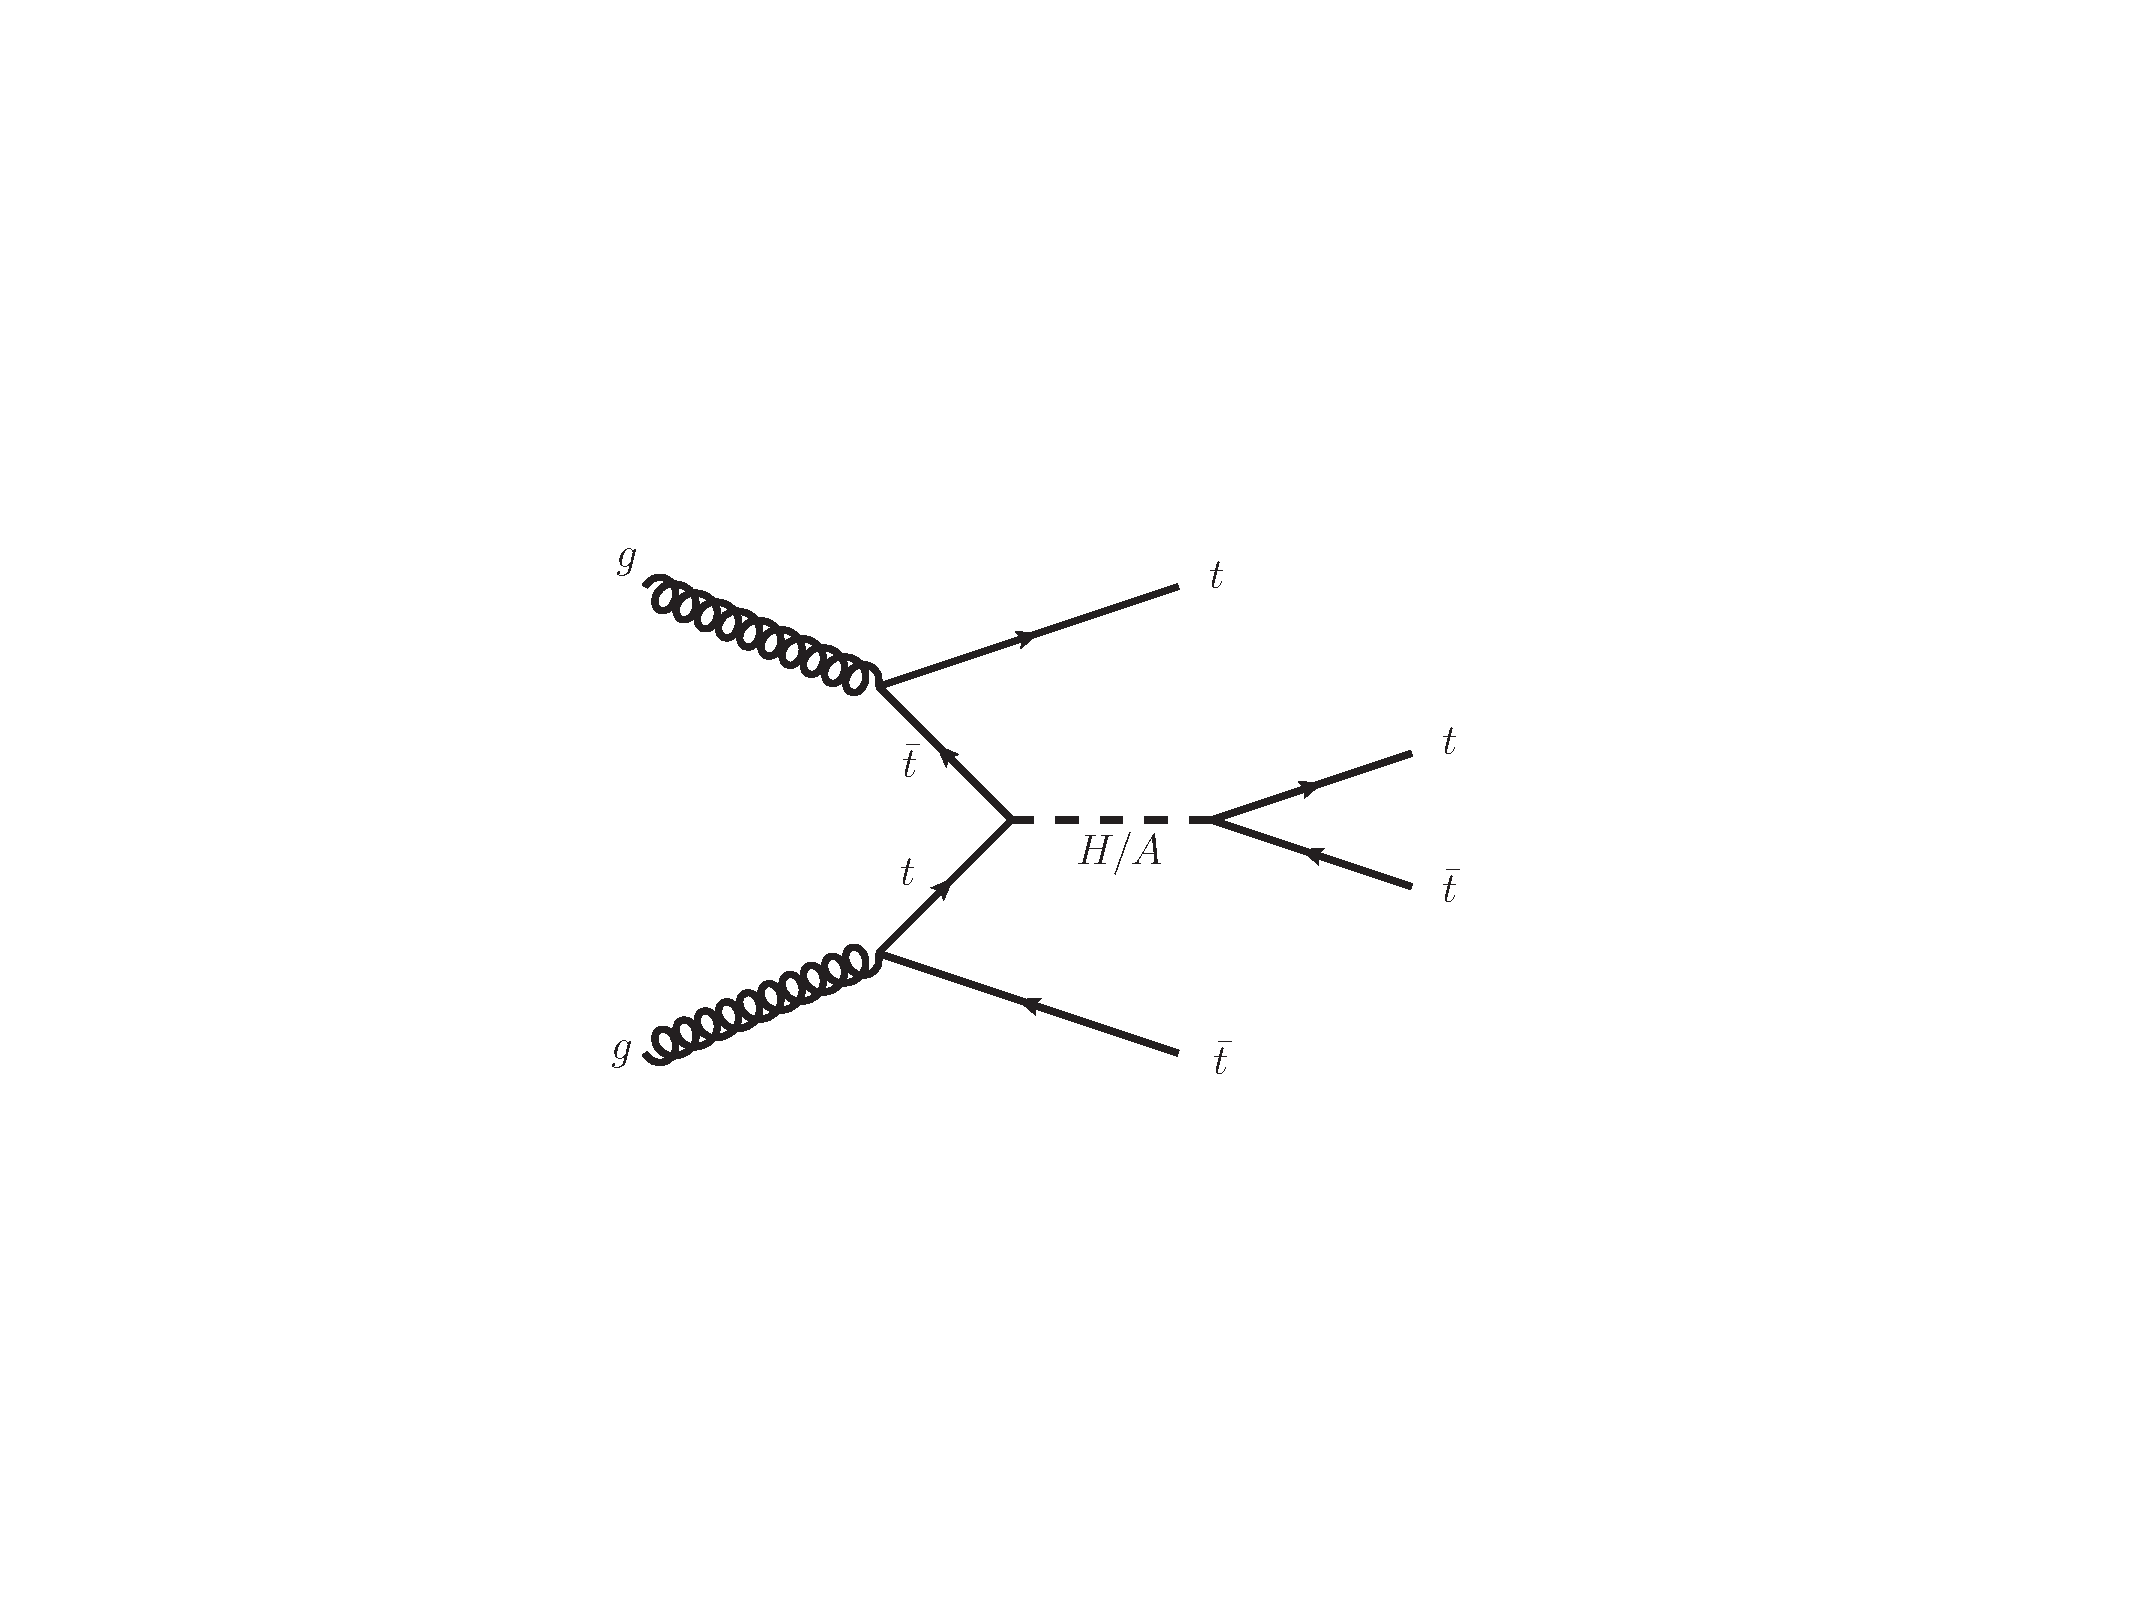
\includegraphics[width=0.43\textwidth]{figures/signal_modeling/hbsm_dia_tth.pdf} \\
    \end{tabular}
     \caption{Example of Feynman diagram for \ttH\ production; the diagrams involving the production of a CP-odd Higgs boson are equivalent.}
   \label{fig:dia}
  \end{center}
\end{figure}

The \ttH\ signal is generated in Type-II 2HDM.  

The signal MC samples are used to describe the kinematics of the signal processes of interest, and they are 
normalised according to the benchmark cross sections described in Sect.~\ref{sec:signal_cross_sections}.

\subsection{Signal generation details}

The signal generation is performed at leading order with \MadG\ from the AtlasProduction release 19.2.5.38.\footnote{https://twiki.cern.ch/twiki/bin/viewauth/AtlasProtected/MadGraph5aMCatNLOForAtlas\#Release\_history}. Only the production via the $s$-channel is considered. The impact of the $t$-channel has been documented in  Appendix~\ref{app:t_channel}. Although the impact on the final results was not investigated, the impact on kinematic distributions was found to be around 10\%, and the $t$-channel has been neglected in this search. All the signal samples are normalised to a cross section of 12 fb. This is the excess between the ATLAS measurement of the cross section of the SM four-top-quark production (24 fb) \cite{Aad:2020klt} and the SM prediction of four-top-quark production (12 fb). This signal normalization is used in the blinding strategy in which we blind all bins with $S/B>5\%$.

The samples are generated in 2HDM-typeII as implemented in the \MadG\ generator\footnote{http://atlas.web.cern.ch/Atlas/GROUPS/COMPUTING/links/releaseDirectory/19.2.5/madgraph/MG5\_aMC\_v2\_3\_3/models/2HDMtypeII/}.
The generated Monte Carlo samples use $\beta=10$ [rad.] and no mixing between the H/A-bosons, therefore the H/A bosons are simultaneously mass and CP eigenstates.
At leading order the kinematics of the investigated BSM processes doesn't depend on the value of $\beta$ coupling, this was confirmed by truth level 
studies~(see Appendix~\ref{app:tan_beta_dep}).
%~\footnote{This was documented on slide 14\\ https://indico.cern.ch/event/479524/contributions/1999037/attachments/1217207/1777909/h\_to\_fermions\_meeting\_2.pdf.}.

The matrix-element calculation is performed at leading order in four-flavour-number scheme and takes into account the spin correlation of all decay products of the W-bosons and top-quarks. The four-flavour parton distribution function set NNPDF31$\_$lo$\_$as$\_$0118 PDFs. is used. \MadG\ is interfaced to \pythiaeight\ for the parton-shower, hadronisation and underlying event simulation. \pythiaeight\ uses the A14-tune; the \EvtGen\ v.1.2.0 program is used to model the properties of the bottom and charm hadron decays.  
In order to increase the available statistics of the generated samples, events are filtered with a single-lepton filter. 
All W-bosons decays are considered, including the decays in tau-leptons.
The event generation is performed for the heavy Higgs-boson mass points shown in Tab.~\ref{tab:MassWidth}; for each mass point, the Higgs-boson width is chosen according to Ref.~\footnote{https://twiki.cern.ch/twiki/pub/AtlasProtected/MSSMbbHSampleProductionMG5aMC/ChoiceOfWidth.txt}. 

For the probed 2HDM parameter space, especially at low $\tan\beta$ ($\tan\beta\leq 0.5$) and high 
Higgs boson mass ($m_{H}\geq 700$ GeV)~\cite{Orlando:2258130} the total width increases up to a few hundreds GeV. 
In order to confirm the limited dependence of the kinematics of the final state particles corresponding to different total width values, 
a check is performed at truth level. A set of truth level \ttH\ samples are generated for $m_{H}=400$~GeV and total width of 
$5$~GeV, $10$~GeV, $100$~GeV, $200$~GeV and $300$~GeV. Particle level objects are used as defined in the TRUTH1 derivations. 
Fig.~\ref{figure:2hdm-width-check} shows the particle level $p_{T}$ distributions for the charged leptons (electrons and muons separately) as well as for the neutrinos and
jets; the typical change in the $p_{T}$ spectrum is of the order of $10\%$, other distributions are unaffected. The impact on the final fit results was not investigated.

The signal acceptance and kinematics dependence of the signals from the Higgs boson total width is not considered in the following results. 

\begin{figure}[tbp]
  \begin{center} \setlength{\tabcolsep}{2.5pt}\footnotesize
    \begin{tabular}{cc}
	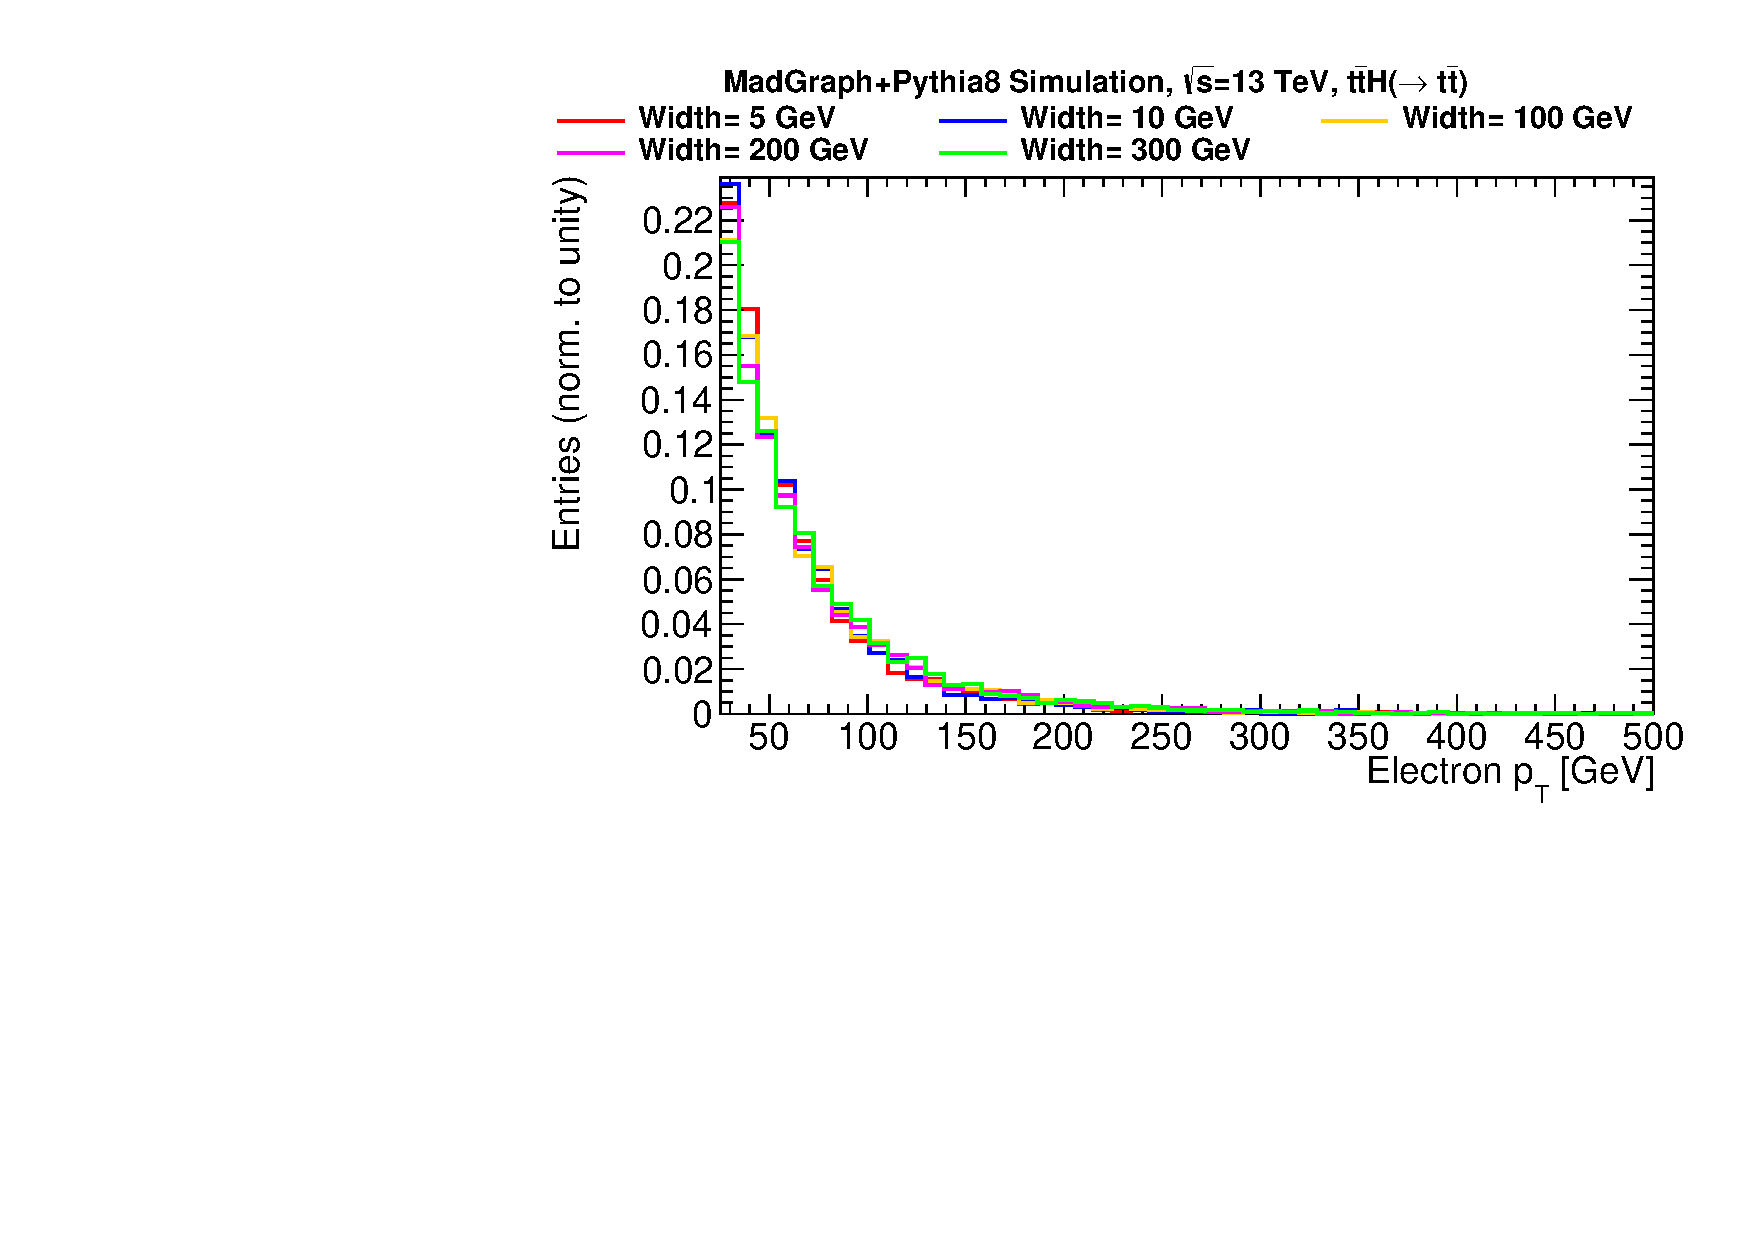
\includegraphics[width=0.43\textwidth]{figures/signal_modeling/width_checks/width_checks_v1_truth_1/plot_n_electrons_pt} &
	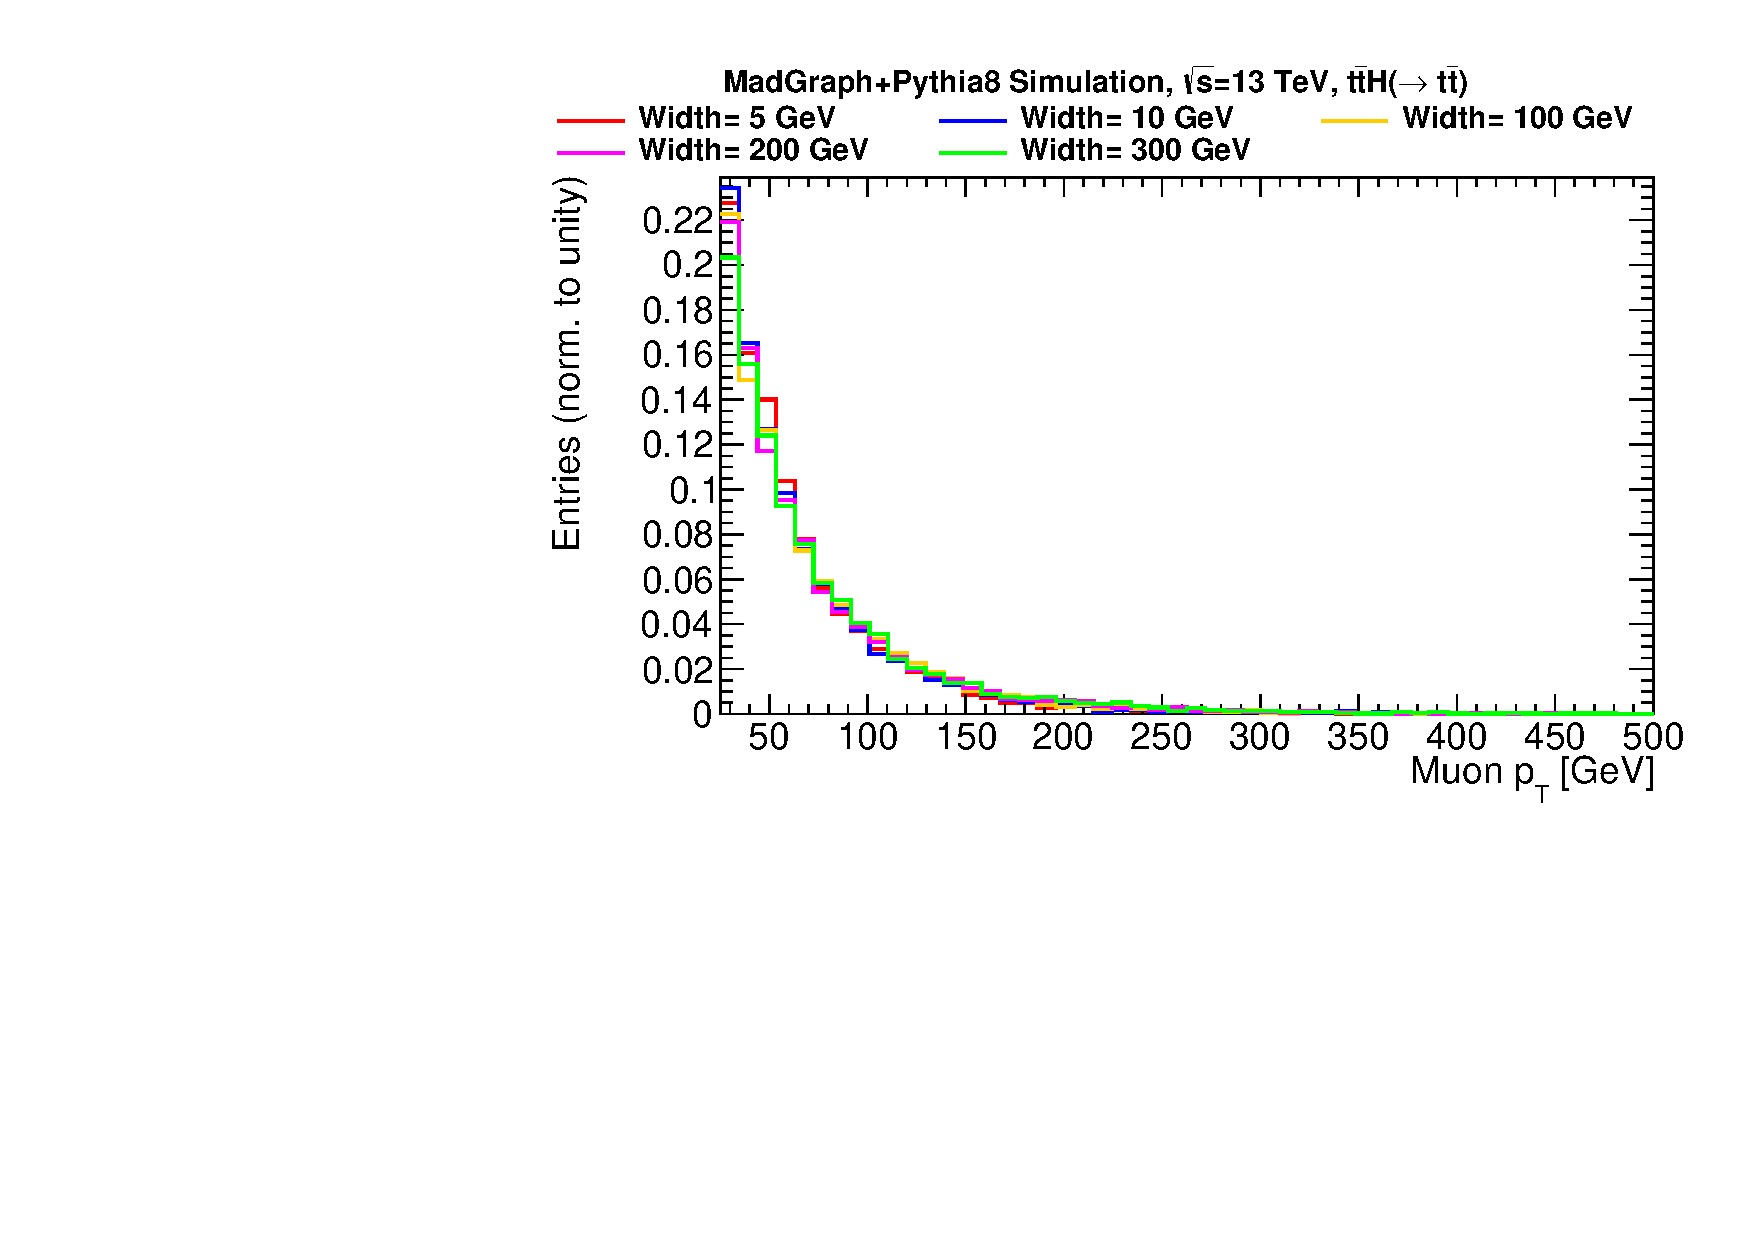
\includegraphics[width=0.43\textwidth]{figures/signal_modeling/width_checks/width_checks_v1_truth_1/plot_n_muons_pt} \\
	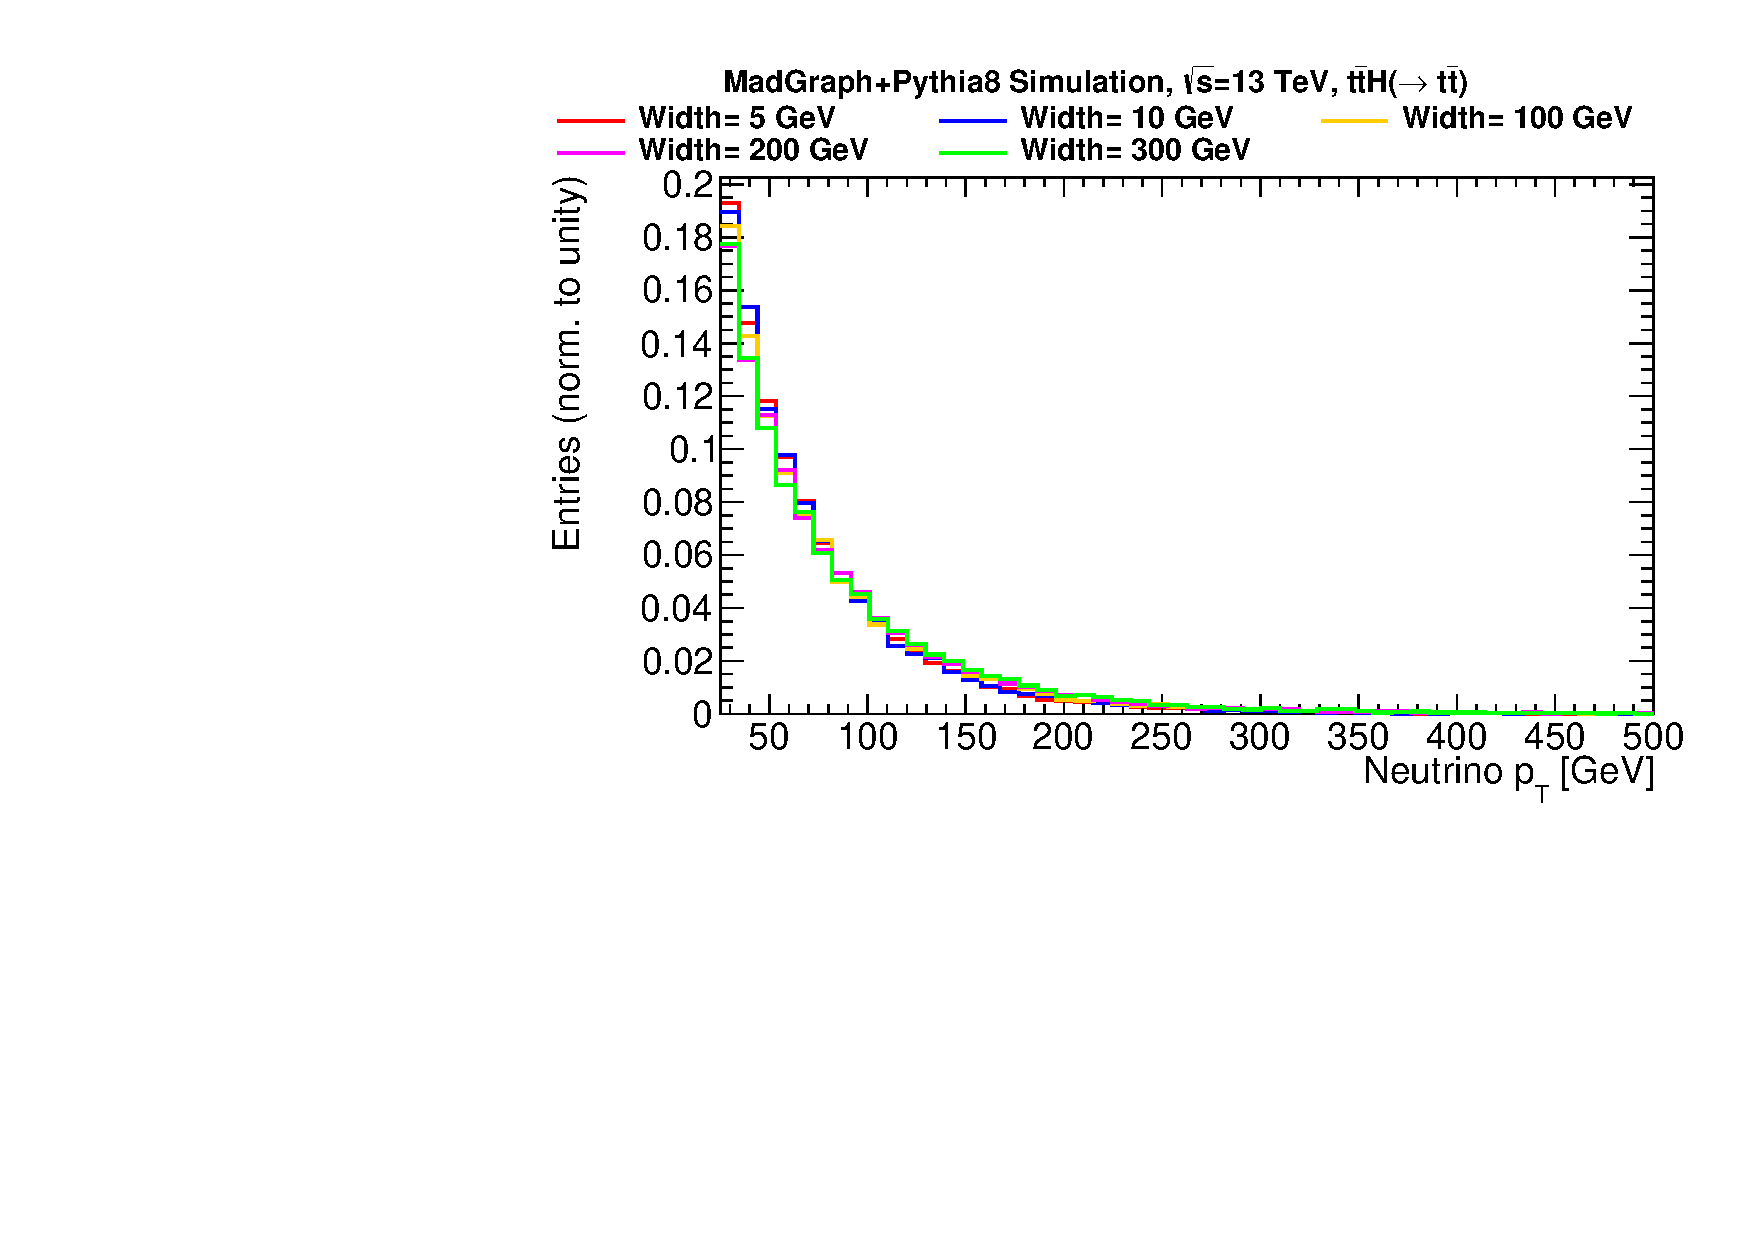
\includegraphics[width=0.43\textwidth]{figures/signal_modeling/width_checks/width_checks_v1_truth_1/plot_n_neutrinos_pt} &
	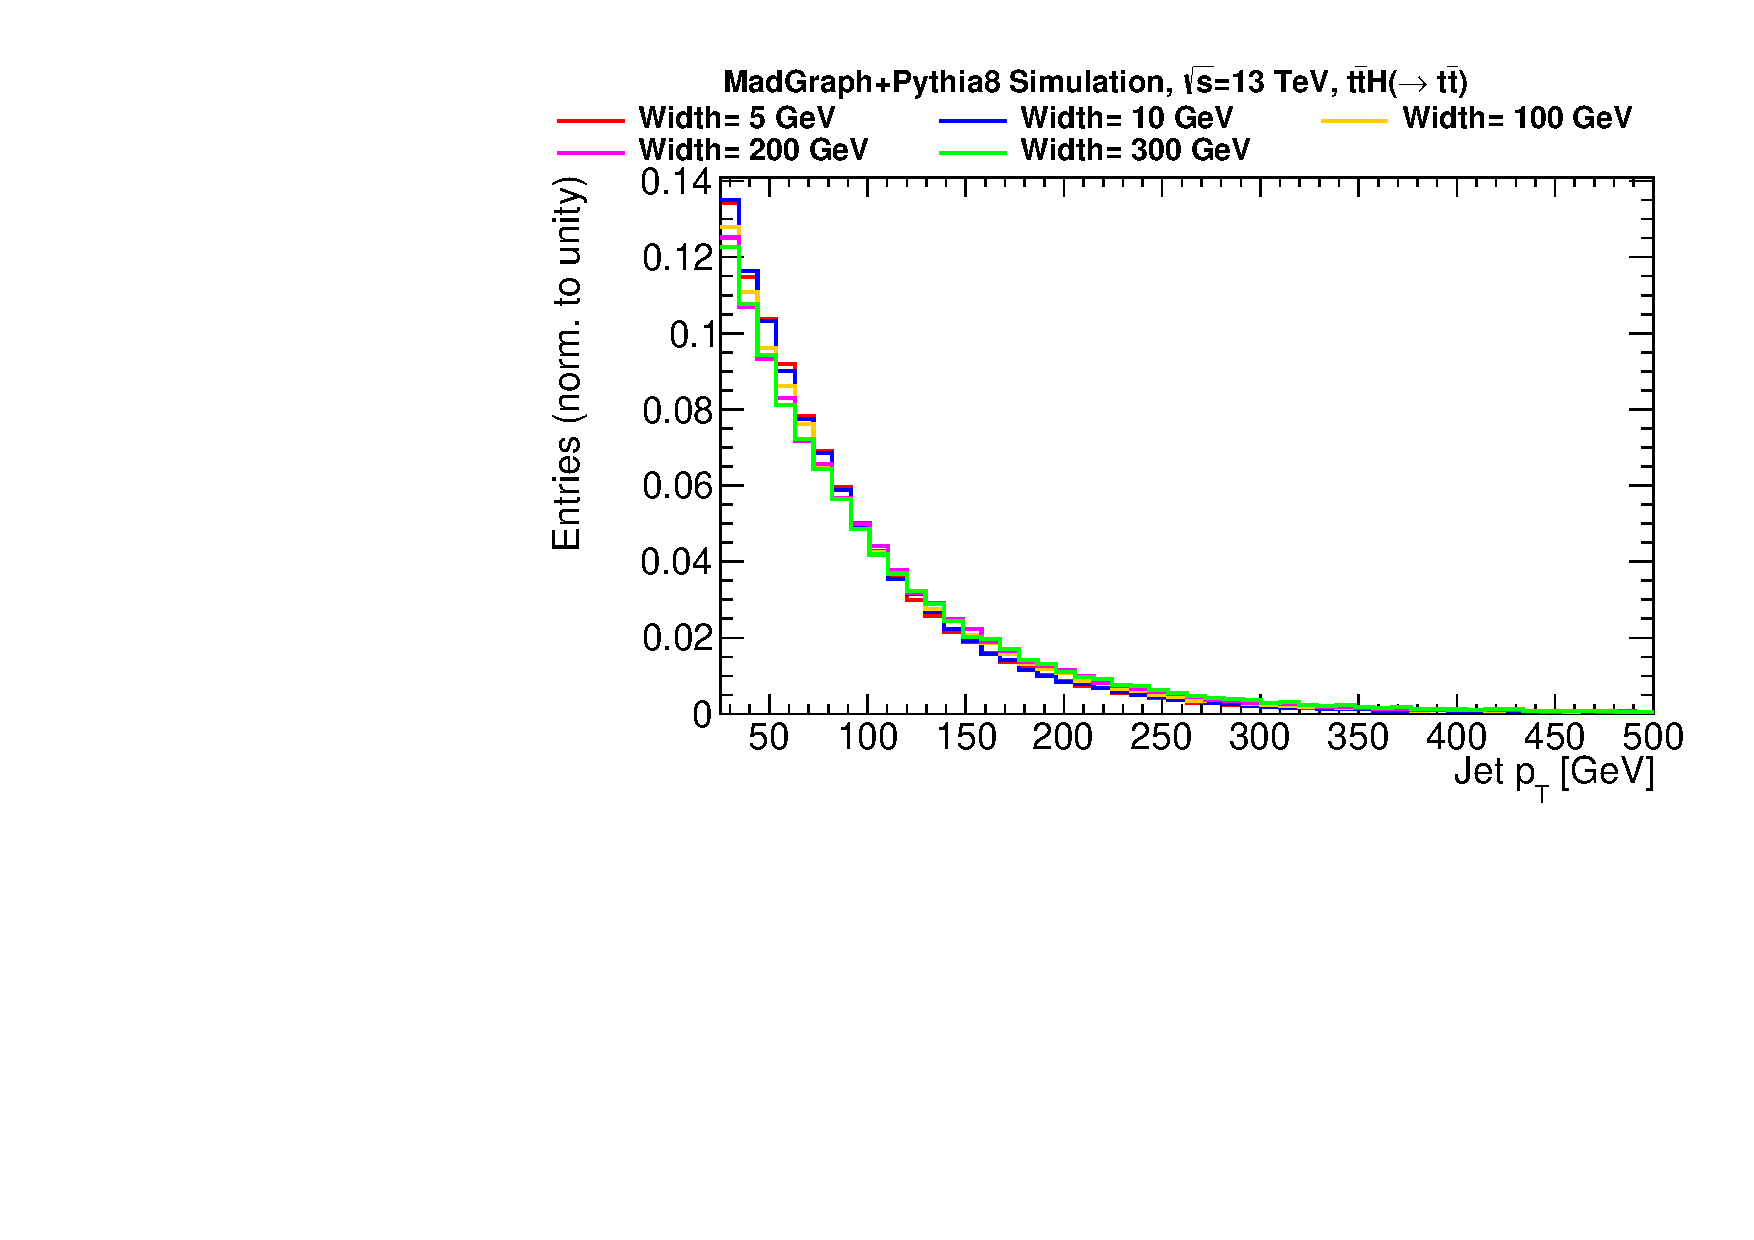
\includegraphics[width=0.43\textwidth]{figures/signal_modeling/width_checks/width_checks_v1_truth_1/plot_n_wzjets_pt} \\
    \end{tabular}
     \caption{Dependence final state particles $p_{T}$ corresponding to different total width values for $m_{H}=400$~GeV. Electrons and Muons are shown at the top, neutrinos and jets at the bottom.}
   \label{figure:2hdm-width-check}
  \end{center}
\end{figure}

The other free parameters of the model don't affect the kinematics and follow the default setting of \MadG.

\begin{table}[!ht]
 \begin{center}\small
    \begin{tabular}{|cccccccccc|}
       \hline
       \multicolumn{10}{|c|}{Mass points [GeV]}\\
        \hline
       200 & 300& 400& 500& 600& 700& 750& 800& 900& 1000\\
       \hline   
       \hline
       \multicolumn{10}{|c|}{Widths [GeV]}\\
        \hline
       1 & 2 & 5& 5& 10& 20& 20& 20& 20& 30\\
       \hline   
\end{tabular}
  \caption{Mass points and widths used for the \ttH\ signal generation.}
  \label{tab:MassWidth}
  \end{center}
\end{table}

\subsection{Interference with the Standard Model background}

Interference effects between the generated BSM signals and the Standard Model background are expected whenever the initial and final state 
particles/partons are the same in the two cases. For the signals introduced in this section, interference might occur with Standard Model four-tops production. 

Studies of the interference effects relevant for this analysis were reported in~\cite{Orlando:2258130}. Interference effects are observed to be at most of the order 
of $20\%$ at parton level, affecting mostly the invariant mass distribution of the Higgs decay products for large width signal scenarios (up to total widths of the order of 100 GeV). Other kinematic distributions, more similar to what used in the final analysis, are affected to a lower extent. As illustration, Figure~\ref{fig:ttHtt:ttfromHm_main} shows  
the invariant mass of the heavy neutral scalar in \ttH\ events with and without taking into account the interference with Standard Model four-top background, 
corresponding to different Higgs boson mass and total width values.  

\begin{figure}[ht]
\begin{center}
\begin{tabular}{ccc}
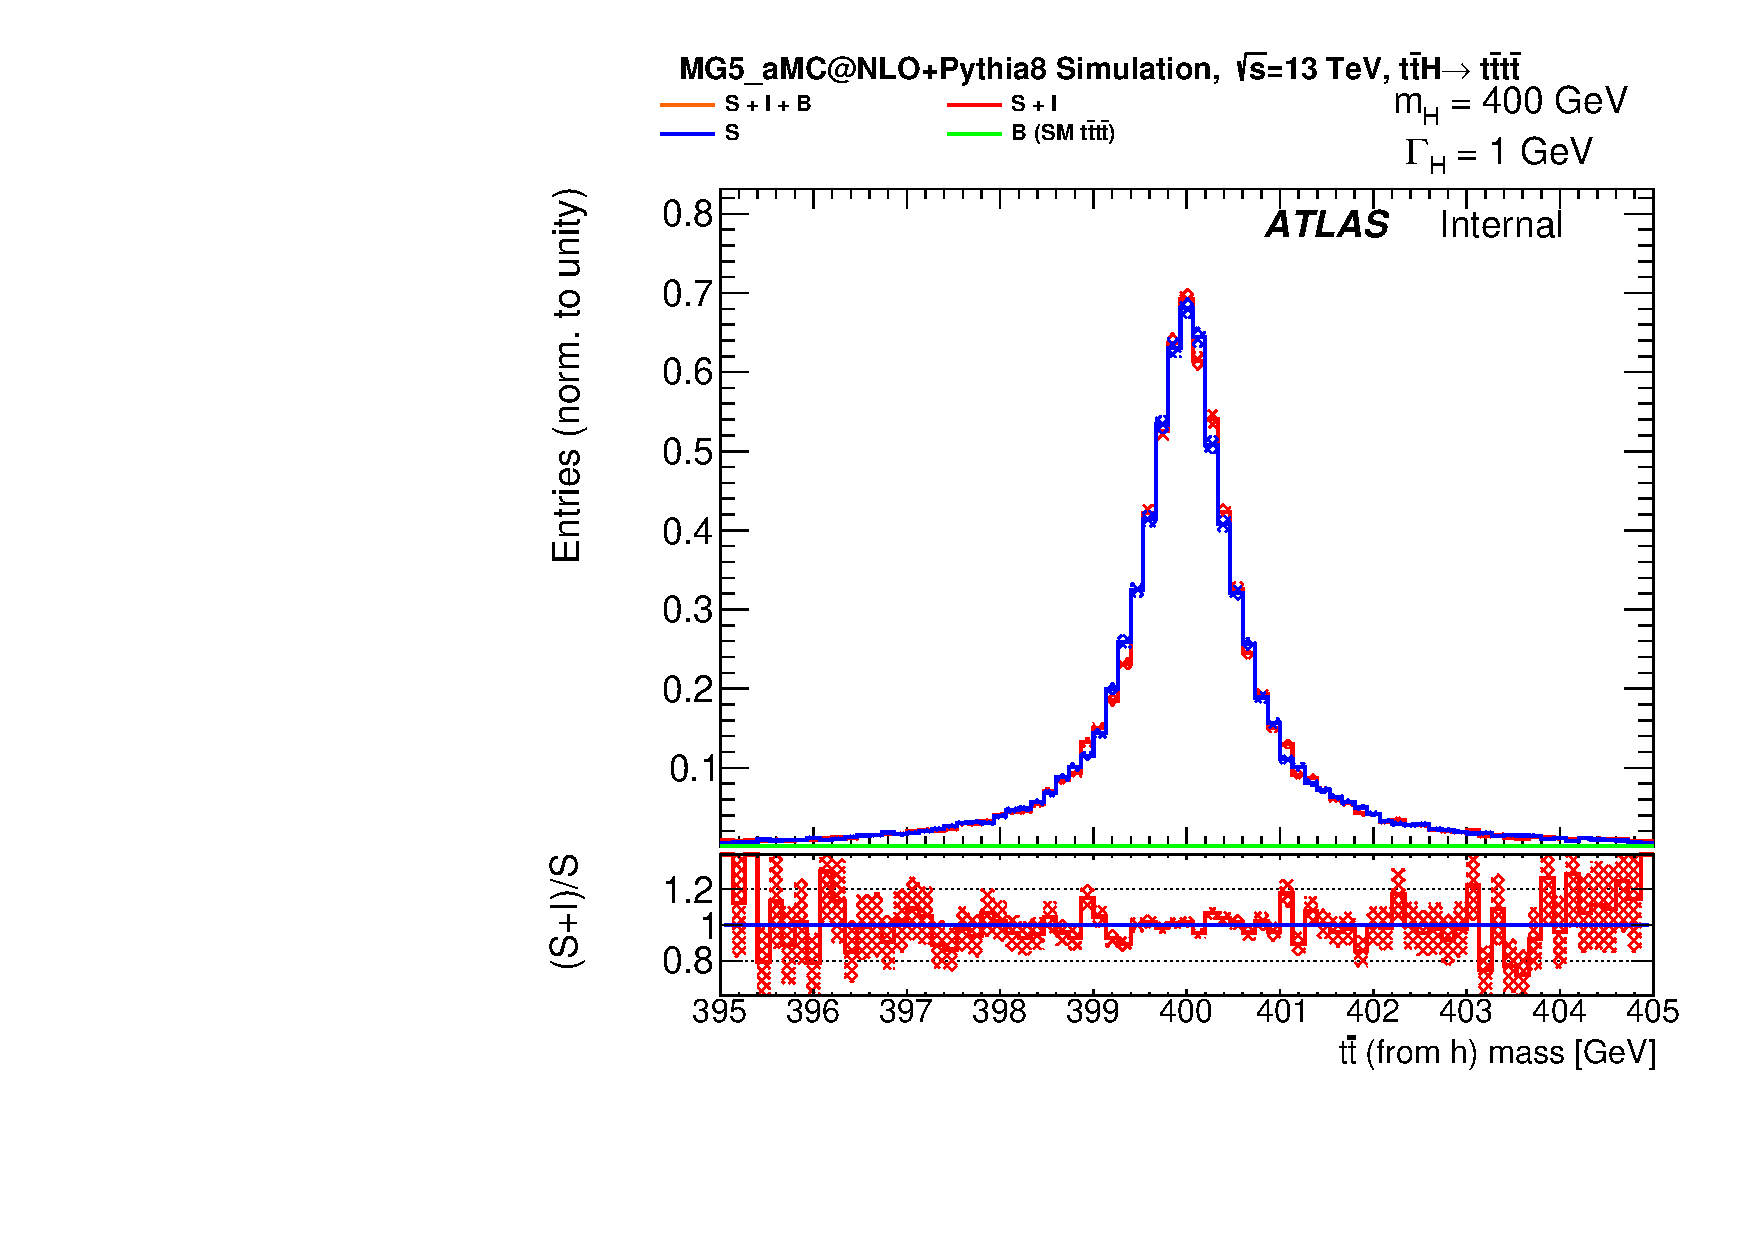
\includegraphics[width=0.315\textwidth]{figures/ttHtt_interf/400_1/plot_n_parton_ttfromH_m.pdf} &

\includegraphics[width=0.315\textwidth]{figures/ttHtt_interf/400_50/plot_n_parton_ttfromH_m.pdf} &

\includegraphics[width=0.315\textwidth]{figures/ttHtt_interf/400_100/plot_n_parton_ttfromH_m.pdf} \\

\includegraphics[width=0.315\textwidth]{figures/ttHtt_interf/500_1/plot_n_parton_ttfromH_m.pdf} &

\includegraphics[width=0.315\textwidth]{figures/ttHtt_interf/500_50/plot_n_parton_ttfromH_m.pdf} &

\includegraphics[width=0.315\textwidth]{figures/ttHtt_interf/500_100/plot_n_parton_ttfromH_m.pdf} \\

\includegraphics[width=0.315\textwidth]{figures/ttHtt_interf/700_1/plot_n_parton_ttfromH_m.pdf} &

\includegraphics[width=0.315\textwidth]{figures/ttHtt_interf/700_50/plot_n_parton_ttfromH_m.pdf} &

\includegraphics[width=0.315\textwidth]{figures/ttHtt_interf/700_100/plot_n_parton_ttfromH_m.pdf} \\

\includegraphics[width=0.315\textwidth]{figures/ttHtt_interf/900_1/plot_n_parton_ttfromH_m.pdf} &

\includegraphics[width=0.315\textwidth]{figures/ttHtt_interf/900_50/plot_n_parton_ttfromH_m.pdf} &

\includegraphics[width=0.315\textwidth]{figures/ttHtt_interf/900_100/plot_n_parton_ttfromH_m.pdf}
\end{tabular}
\caption{Normalized invariant mass distribution of the heavy scalars $H/A$ 
for different width (respectively $1$ GeV (left), $50$ GeV (center) and $100$ GeV (right) ) and mass ($400$ GeV, $500$ GeV, $700$ GeV 
and $900$ GeV, in increasing rows) assumptions. Distributions for signal-only (blue) and signal+interference (red) assumptions are shown (see text). Bands refer to statistical MC uncertainties. The signal is generated assuming $m_{H}=400$~GeV.}
\label{fig:ttHtt:ttfromHm_main}
\end{center}
\end{figure}

Given the limited impact observed on at truth level, no interference effects are considered for this analysis. 

\subsection{Heavy Higgs theoretical predictions}
\label{sec:signal_cross_sections}
The theoretical predictions for the investigated signal processes are described in this sub-section. 
For each mass point available from the generated Monte-Carlo samples, cross sections are evaluated in the relevant parameter-space of the investigated benchmark models.  

The benchmark model we will consider is 2HDM type~II. This model is an ``MSSM-like'' model, in which one Higgs doublet couples to up-type quarks
and the other to down-type quarks and charged leptons. Another common choice from literature is the 2HDM type~I model, but type~I and 
type~II models only differ for their couplings to down-type fermions, thus they predict same cross sections for \ttH\ and \ttA. 

All used cross-sections for heavy neutral Higgs-bosons production are obtained from the standard HBSM recommendations \\
{\small{https://twiki.cern.ch/twiki/bin/viewauth/AtlasProtected/HiggsBSM2HDMRecommendations}} \\
from the LHC HXSG (Higgs Cross-Section working Group). The used version of the cross-sections is 1.6.6\_13TeV; in this version the default cross-sections are derived in the Santander matched 4FS+5FS scheme.

The cross sections in the alignment limit are presented in Fig.~\ref{fig:bench_xsec_ttH_1D}.

\begin{figure}[tbp]
	\begin{center}\setlength{\tabcolsep}{2.0pt}\small   

		\begin{tabular}{cc}
					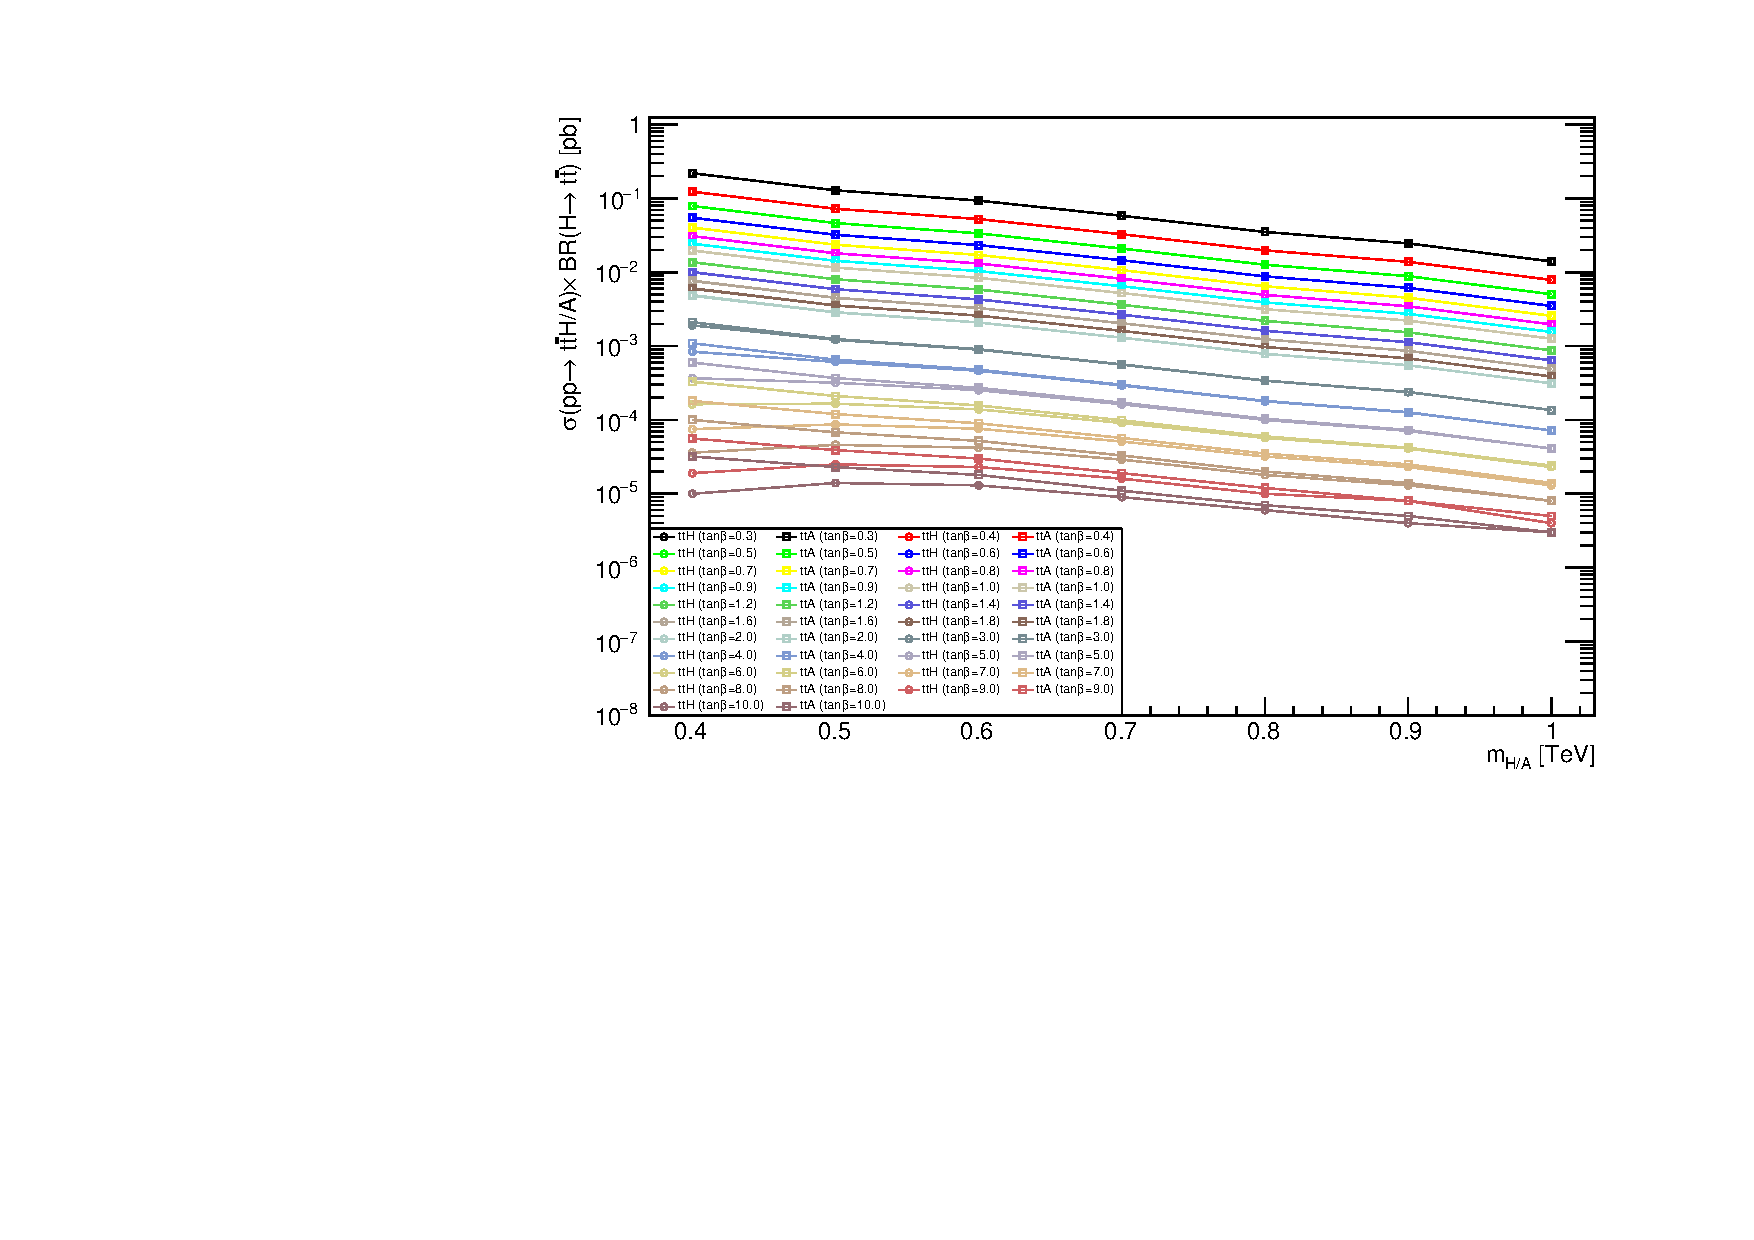
\includegraphics[width=0.47\textwidth]{figures/signal_modeling/hbsm_cross_sections/tanb_mass} 
					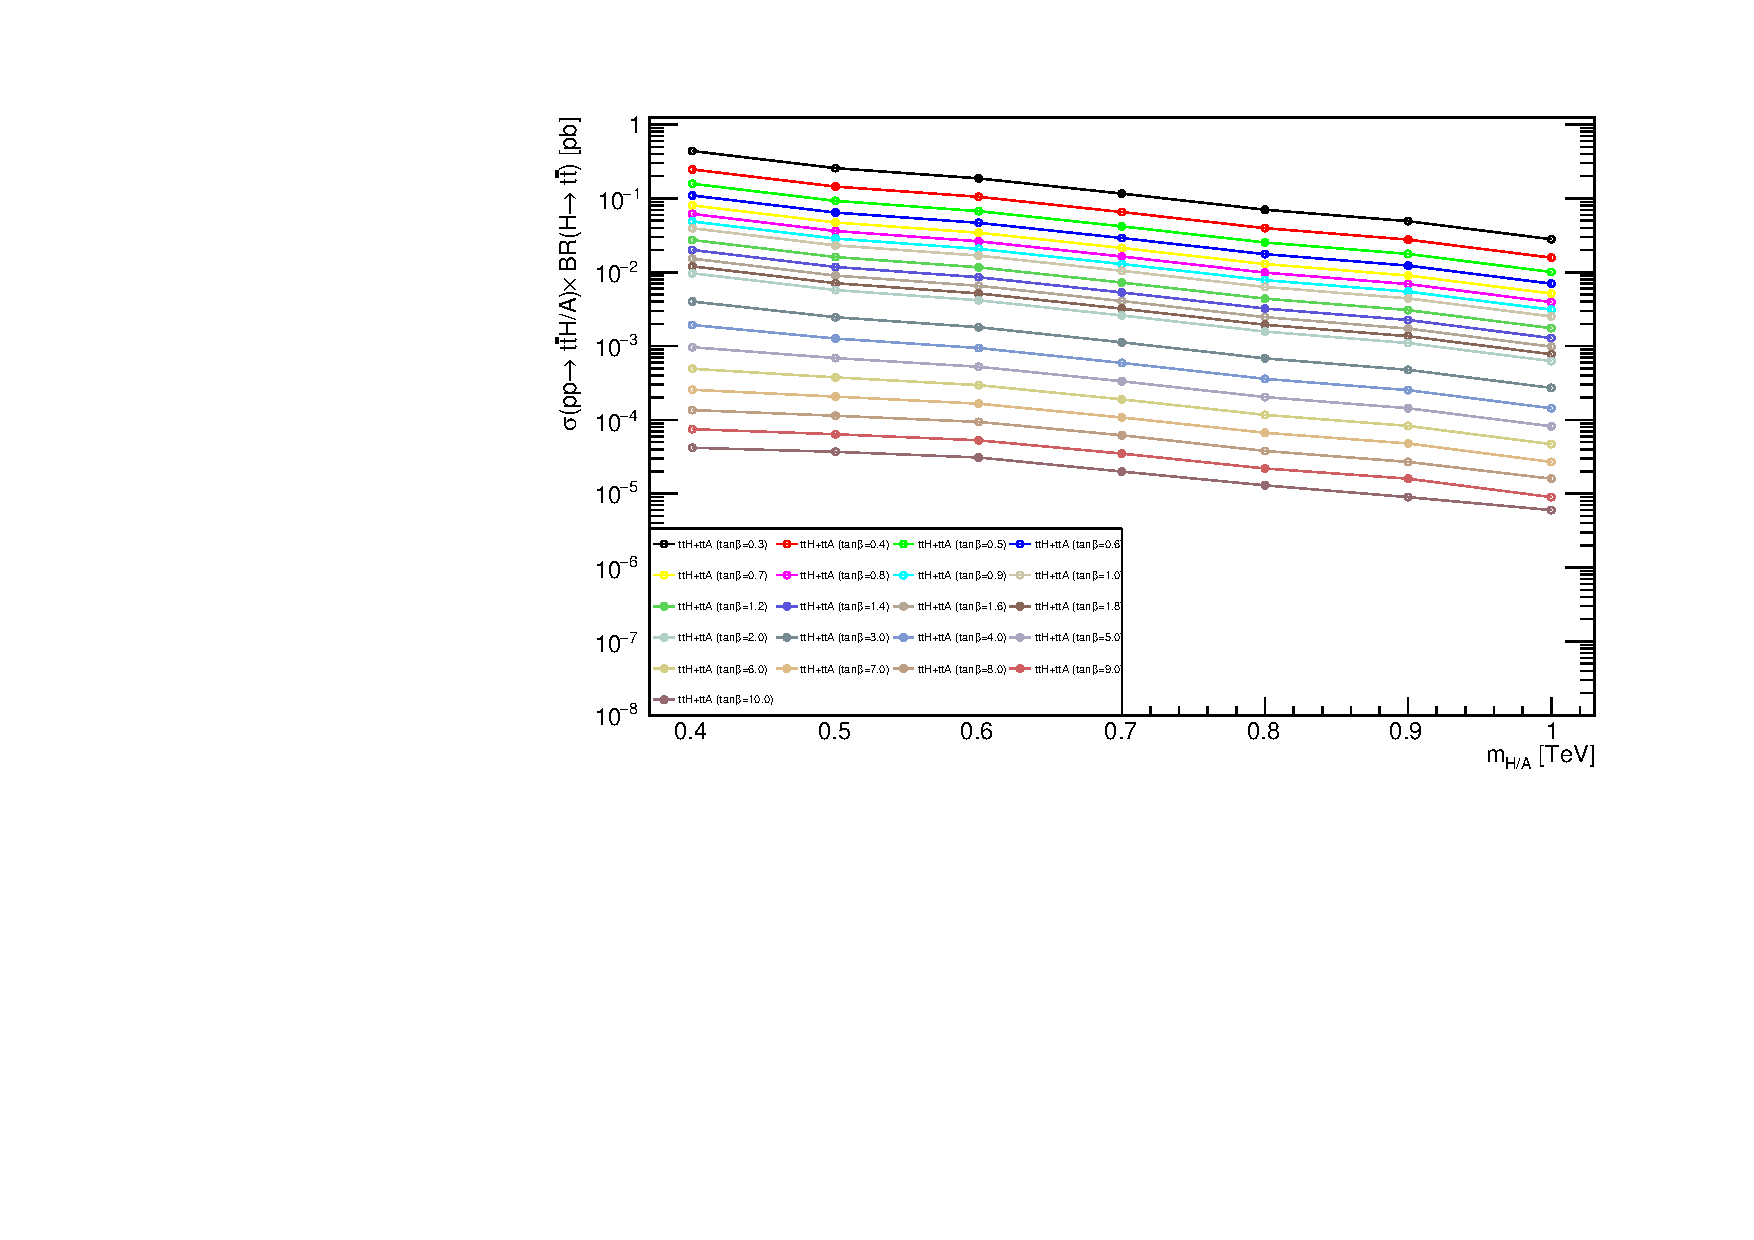
\includegraphics[width=0.47\textwidth]{figures/signal_modeling/hbsm_cross_sections/tanb_mass_merge_ttA_ttH} 
		\end{tabular}
		\caption{Cross-sections times branching-ratios for \ttH\ (left, circle marker), \ttA\ (left, square marker) and $\ensuremath{t\bar{t}H}+\ensuremath{t\bar{t}A}\rightarrow t\bar{t}t\bar{t}$\ (right, circle marker) in 2HDM type~II presented as a funtion of $m_{A}$ for several $\tan\beta$ points in the alignment limit.}
		\label{fig:bench_xsec_ttH_1D}
	\end{center}
\end{figure}



% Daniela, Nicola
%-------------------------------------------------------------------------------


%-------------------------------------------------------------------------------                                                                                                
\FloatBarrier
\section{Samples of simulated events and data}% Daniela, Nicola
\label{sec:samples}
%
The data used in this analysis corresponds to the full LHC Run 2 dataset collected by the ATLAS detector at $\sqrt{s}=13~\tev$
between 2015 and 2018 with stable beam conditions and with all detector systems operating normally.
The average number of additional $pp$ interactions per bunch crossing (pileup) $<\mu>$ ranged between 14 in 2015 and 38 in 2017-2018.
The event quality was checked to remove events with noise bursts or coherent noise in the calorimeters.

The analysis uses single lepton triggers. Table~\ref{tab:slep_trigger} lists the different single lepton triggers used for each data periods.
A matching between online objects firing the trigger and the offline reconstructed object is required.

\begin{table}[!hbt]
\begin{center}
\begin{tabular}{c|c}
\hline
Year of data taking & list of ORed triggers \\
\hline \hline
\multicolumn{2}{c}{single electron triggers} \\
\hline \hline
2015 & e24\_lhmedium\_L1EM20VH, e60\_lhmedium, e120\_lhloose  \\
2016, 2017 and 2018 & e26\_lhtight\_nod0\_ivarloose, 60\_lhmedium\_nod0, e140\_lhloose\_nod0 \\
\hline \hline
\multicolumn{2}{c}{single muon triggers} \\
\hline \hline
2015 & mu20\_iloose\_L1MU15, mu50 \\
2016, 2017 and 2018 & mu26\_ivarmedium, mu50 \\
\hline
\end{tabular}
\caption{List of single lepton triggers used in the analysis per data period.}
\label{tab:slep_trigger}
\end{center}
\end{table}

Monte Carlo simulation is used to estimate the signal acceptance as well as the physics background.
All MC events used in this analysis come from centrally produced MC16a, MC16d and MC16e samples.
The exact list of MC samples used can be found at these gitlab links for 
\href{https://gitlab.cern.ch/atlas-phys/exot/hqt/bsm_h_4t/common-framework/-/blob/master/preProd/mc16a_SM4tops.py}{MC16a}, 
\href{https://gitlab.cern.ch/atlas-phys/exot/hqt/bsm_h_4t/common-framework/-/blob/master/preProd/mc16d_SM4tops.py}{MC16d} 
and \href{https://gitlab.cern.ch/atlas-phys/exot/hqt/bsm_h_4t/common-framework/-/blob/master/preProd/mc16e_SM4tops.py}{MC16e}.  The background samples are described below:

After event preselection, the main background is $\ttbar$+jets production, with the production of a $W$ boson in association with
jets ($W$+jets) and multijet events contributing to a lesser extent. Small contributions arise from single top quark, $Z$+jets and 
diboson ($WW,WZ,ZZ$) production, as well as from the associated production of a vector boson $V$ ($V=W,Z$) or a Higgs boson 
and a $\ttbar$ pair ($\ttbar V$ and $\ttbar H$). Multijet events contribute to the selected sample via the misidentification of a jet or 
a photon as an electron or via the presence of a non-prompt lepton, e.g.~from a semileptonic $b$- or $c$-hadron decay. Studies were made in order to measure the impact of this background and it has proved to be negligible in similar recent analyses. The rest of the background contributions are estimated from simulation 
and normalised to their theoretical cross sections. In the case of the $\ttbar$+jets background prediction, further corrections are 
applied to improve agreement between the data and simulation, as discussed in Sect.~\ref{sec:nn_rew}.

Both signal and background samples also include a simulation of pileup interactions, and are processed through a 
full {\sc Geant4} or fast (AFII) detector simulation and the same reconstruction software as the data. Further details about the modelling of each 
of the backgrounds are provided below. 
%A complete list of the Monte Carlo datasets for background processes used in the analysis is given in App.~\ref{sec:datasets}.  

\begin{description}

\item[\ttbar:] 

The nominal $t\bar{t}$ sample is generated using the {\powheg}
v2 NLO generator~\cite{Nason:2004rx,Frixione:2007vw,Alioli:2010xd} with the
{\textsc NNPDF3.0} parton distribution function (PDF) set~\cite{Ball:2014uwa} using the 5-flavour scheme (5FS). The
$h_{\textrm{damp}}$ parameter, which controls the \pt of the first additional
emission beyond the Born configuration, is set to 1.5 times the top quark mass
of $m_t=172.5$ \gev. The main effect of the $h_{\textrm{damp}}$ setting is to regulate the
high-\pt emission against which the \ttbar system recoils. Parton shower and
hadronisation are modelled by {\textsc Pythia} 8.2~\cite{Sjostrand:2007gs} with
the appropriate A14~\cite{ATLASUETune4} tune. 
The sample includes event
weights so that we can evaluate uncertainties from the choice of scales 
and the PDF used. The sample is
generated separately for ``non-all hadronic'' $W$ bosons decays, dilepton decays,
and all-hadronic decays. The dilepton sample is a subset of the first sample.
Additional samples for each of these types of $W$ bosons decays are generated with
filters requiring extra $b$ jets or large H$_{T}$, which is important to ensure a reasonable
number of simulated events passing cuts in the high $b$-tag multiplicity region and ensure enough statistics at large H$_{T}$.

An additional \ttbin~sample was produced with the \powhegboxRes~\cite{Jezo:2018yaf} NLO
generator and \openloops~\cite{Cascioli:2011va,Denner:2016kdg}, using a pre-release of the implementation of this process in \powhegboxRes\
provided by the authors~\cite{ttbbPowheg}, with the \texttt{NNPDF3.0nlonf4}~\cite{Ball:2014uwa} PDF set, and using \textsc{Pythia8} for the PS and hadronisation. 
This sample was produced in the four flavour scheme with $m_b=4.95$~\GeV~in the matrix element. 
This will be referenced in text as \ttbin~(4FS), and will be included as systematic in the fit modeling. 


Additional types of samples are generated for studying systematic uncertainties
on the \ttbar\ backgrounds. The Monte Carlo generator uncertainty for the hard
process is evaluated by comparing the default \textsc{Powheg+Pythia8} sample to
one generated by \amcatnlo\ interfaced to \textsc{Pythia} 8.
The showering and hadronisation uncertainties compare the default \textsc{Powheg+Pythia8} sample
to one where Powheg is interfaced instead to Herwig 7.0.4~\cite{Bellm:2015jjp,Bahr:2008pv}. Radiation systematics 
are evaluated following PMG recommendations outlined here \href{https://twiki.cern.ch/twiki/bin/view/AtlasProtected/PmgTopProcesses\#Systematic\_uncertainties}{TopPMG};
these are based upon built-in Monte Carlo event weights implemented in the nominal \textsc{Powheg+Pythia8} sample and an alternative version of 
\textsc{Powheg+Pythia8} with factorisation ($\mu_{F}$) and renormalisation scales ($\mu_{R}$) set to 0.5 times their values in the default sample \textsc{Powheg+Pythia8} and varied tune of the parton-shower model.

Some \ttbar\ samples mentioned above are studied in detail and compared in~\cite{ATL-PHYS-PUB-2022-026}.

These samples are normalised to the top++2.0~\cite{Czakon:2011xx} theoretical cross
section of $832^{+46}_{-51}$~pb, calculated at next-to-next-to-leading order
(NNLO) in QCD that includes resummation of next-to-next-to-leading logarithmic
(NNLL) soft gluon terms~\cite{Cacciari:2011hy,Baernreuther:2012ws,Czakon:2012zr,Czakon:2012pz,Czakon:2013goa}.
Theoretical uncertainties result from variations of the factorisation and
renormalisation scales, as well as from uncertainties on the PDF and
$\alpha_{S}$. The latter two represent the largest contribution to the overall
theoretical uncertainty in the cross section and were calculated using the
PDF4LHC prescription.

The $\ttbar$ events are categorised
depending on the flavour of partons that are matched to particle jets that do
not originate from the decay of the $\ttbar$ system. Particle jets are
reconstructed from all stable truth particles (not counting muons and neutrinos)
with the anti-$k_t$ algorithm with a radius parameter $R=0.4$ and are required
to have $\pt>15\,\gev$ and $|\eta|<2.5$. Events where at least one such particle
jet is matched within $\Delta R<0.3$ to a $b$-hadron with $\pt>5\,\gev$ not
originating from a top quark decay are labelled as \ttbin\ events. Similarly,
events which are not already categorised as \ttbin, and where at least one
particle jet is matched to a charm quark not originating from a $W$ bosons decay,
are labelled as \ttcin\ events.
Events labelled as either \ttbin\  or \ttcin\ are generically referred to as
\ttbar+HF events (HF for ``heavy flavour'').  The remaining events are labelled
as $\ttbar$+light-jet events, including those with no additional jets. All these samples
are generated by using fast simulation (AFII)

\item[\tttt:] The production of \tttt\ events is modelled using the \amcatnlo~v2.6.2 \cite{Alwall:2014hca} generator which provides matrix elements at next-to-leading order~(NLO) in the strong coupling constant \alphas with the NNPDF3.1 NLO~\cite{Ball_2017} parton distribution function.
The functional form of the renormalisation and factorisation scales are set to $\mu_r=\mu_f=m_\textrm{T}/4$ where $m_\textrm{T}$ is defined as the scalar sum of the transverse masses $\sqrt{m^2+p^2_{T}}$  of the particles generated from the matrix element calculation, following Ref.~\cite{Frederix:2017wme}.
Top quarks are decayed at LO using \madspin~\cite{Frixione:2007zp,Artoisenet:2012st} to preserve all spin correlations.
The events are interfaced with \pythiaeight.230~\cite{Sjostrand:2014zea} for the parton shower and hadronisation, using the A14 set of tuned parameters~\cite{ATL-PHYS-PUB-2014-021} and the NNPDF2.3 LO~\cite{Ball_2013} PDF set.
The decays of bottom and charm hadrons are simulated using the \EvtGen\ v1.6.0 program~\cite{EvtGen}.
To avoid the use of negative weights in the Boosted Decision Trees training, an additional \tttt\ sample is produced at leading order (LO) with the same MC settings used for the NLO sample. 
Another \tttt\ sample is also produced at NLO replacing the parton shower of the nominal samples to \herwigseven.04~\cite{Bahr:2008pv,Bellm:2015jjp} to evaluate the impact of the parton shower and hadronisation model. The H7UE set of tuned parameters~\cite{Bellm:2015jjp} and the MMHT2014LO PDF set~\cite{Harland-Lang:2014zoa} are used for this sample. The ATLAS detector response is simulated using AltFastII (AFII). 
All \tttt\ samples are normalized to cross section of 13.37 fb based on the NLO (QCD+EW) + NLL' prediction from Ref.~\cite{vanBeekveld:2022hty}.


\item[\ttV:]  
Samples of $\ttbar V$ events, with the matrix element calculation performed up to two additional partons at LO, and of  $\ttbar WW$ events,
are generated using {\MadG} and interfaced to \textsc{Pythia} 8 with the A14 NNPDF23LO UE tune. 
Showering is performed using \textsc{Pythia} 8.210 and the A14 tune.

\item[$t\bar tH$:] The production of $t\bar tH$ events is modelled using the \powheg v2~\cite{Frixione:2007nw,Nason:2004rx,Frixione:2007vw,Alioli:2010xd} generator at NLO with the NNPDF3.0 NLO~\cite{Ball:2014uwa} PDF set. The \powheg model parameter $h_{damp}$, which controls the matrix element to parton shower matching and effectively regulates the high-\pT  radiation, is set to $1.5\times ( 2m_t +m_H)/2$, where $m_H=125$~\GeV. 
The parton shower and hadronisation were modelled with  \pythiaeight.230~\cite{Sjostrand:2014zea}~ using the A14 tune~\cite{ATL-PHYS-PUB-2014-021} and the NNPDF2.3 LO~\cite{Ball_2013} PDF set.  The simulated sample is normalised to the cross section computed at NLO in QCD with the leading NLO electroweak corrections~\cite{Frixione:2015zaa,deFlorian:2227475}. An alternative sample generated with \amcatnlo~v2.3.3 has been used to evaluate the generator uncertainty. 


\item[Single-top:]  Single-top $tW$ associated production is modelled using the \powheg~\cite{Re:2010bp,Nason:2004rx,Frixione:2007vw,Alioli:2010xd}~v2 generator at NLO in QCD in the five flavour scheme with the NNPDF3.0 NLO~\cite{Ball:2014uwa} PDF set.
The diagram removal scheme~\cite{Frixione:2008yi} was employed to handle the interference with \ttbar\ production~\cite{ATL-PHYS-PUB-2016-020}.
Single-top t-channel production is modelled using the \powheg\,\cite{Frederix:2012dh,Nason:2004rx,Frixione:2007vw,Alioli:2010xd}~v2 generator at NLO in QCD in the four flavour scheme with the NNPDF3.0 NLOnf4~\cite{Ball:2014uwa} PDF set.
Single-top s-channel production is modelled using the \powheg~\cite{Alioli:2009je,Nason:2004rx,Frixione:2007vw,Alioli:2010xd}~v2 generator at NLO in QCD in the five flavour scheme with the NNPDF3.0 NLO~\cite{Ball:2014uwa} PDF set.
For all single-top processes, the events are interfaced with \pythiaeight.230~\cite{Sjostrand:2014zea} using the A14 tune~\cite{ATL-PHYS-PUB-2014-021} and the NNPDF2.3 LO PDF set.

\item[$V$+jets:] The production of $V+$jets is simulated with the \sherpa~v2.2.1~\cite{Bothmann:2019yzt}
generator using NLO-accurate matrix elements for up to two jets, and LO-accurate matrix elements
for up to four jets calculated with the Comix~\cite{Gleisberg:2008fv}
and OpenLoops~\cite{Cascioli:2011va,Denner:2016kdg} libraries. They
are matched with the \sherpa parton shower~\cite{Schumann:2007mg} using the MEPS@NLO
prescription~\cite{Hoeche:2011fd,Hoeche:2012yf,Catani:2001cc,Hoeche:2009rj}
using the set of tuned parameters developed by the \sherpa authors.
The NNPDF3.0 NNLO set of PDFs~\cite{Ball:2014uwa} is used and the samples
are normalised to a next-to-next-to-leading order (NNLO)
prediction~\cite{Anastasiou:2003ds}.

\item[$VV$:] Samples of diboson final states ($VV$) are simulated with the
\sherpa~v2.2.1 or v2.2.2~\cite{Bothmann:2019yzt} generator depending on the process.
Fully leptonic final states and semileptonic final states, where one boson
decays leptonically and the other hadronically, are generated using
matrix elements at NLO accuracy in QCD for up to one additional parton
and at LO accuracy for up to three additional parton
emissions. Samples for the loop-induced processes $gg \to VV$ are
generated using LO-accurate matrix elements for up to one
additional parton emission for both cases of fully leptonic and
semileptonic final states. The matrix element calculations are matched
and merged with the \sherpa parton shower based on Catani-Seymour
dipole~\cite{Gleisberg:2008fv,Schumann:2007mg} using the MEPS@NLO
prescription~\cite{Hoeche:2011fd,Hoeche:2012yf,Catani:2001cc,Hoeche:2009rj}.
The virtual QCD correction are provided by the
\openloops\ library~\cite{Cascioli:2011va,Denner:2016kdg}. The
NNPDF3.0 NNLO set of PDFs is used~\cite{Ball:2014uwa}, along with the
dedicated set of tuned parton-shower parameters developed by the
\sherpa authors.

\item[$S_8S_8\rightarrow t \bar tt \bar t$:] The results of this analysis  are reinterpreted in the context of a simplified model  which  considers a scalar state $S_8$ decaying to a pair of top quarks  ($S_8 \rightarrow t \bar t$), 
giving as a final state  $t \bar tt \bar t$ events \cite{Darm__2021}.
The field $S_8$ is color-octet with respect to $SU(3)_{C}$.
The new physics Lagrangian for the real scalar field $S_8$ is given by

\begin{equation}
\mathcal{L}_{S8} = \frac{1}{2}D_\mu S_{8}^{A}D^{\mu}S_{8}^{A}- \frac{1}{2} m^2_{S8}S_{8}^{A}S_{8}^{A} + \bar{t} [y_{8S}+i y_{8P}\gamma^{5}]T^{A}S_{8}^{A}t,
\end{equation}

where $T^A$ represent the generators of $SU(3)$ in the fundamental representation, 
$m_{S8}$ the mass of $S_8$, and  the scalar $y_{8S}$ and pseudo-scalar $y_{8P}$,  the interactions of the $S_8$ state with the top quark.  
Any higher-dimensional operator coupling the scalar-octet state to gluons are ignored.  
  The usual QCD interactions of the scalar field are included through the covariant derivatives used for the kinetic term. 
  The case of a purely scalar  $S_8$ field, considered in this work, is obtained by setting $y_{8P}$  to zero.
  
  Events were generated at leading order with MadGraph5$\_$aMC@NLO, with the decay of $S_8\rightarrow t \bar t$ handled by MadSpin. 
  Further decay and showering is  performed with Pythia8.   
  The parameter $y_{8S}$ is set to $0.1$, ensuring that only the pair production of the color-octet $S_8$,  $pp\rightarrow S_8S_8$,  dominates.  
  Under this kinematic regime, the interference with the SM background and the $ t \bar tS_8$ production contribute  less than 10\% to the total BSM $t \bar tt \bar t$ production for  $m_{S8}<2$ TeV.  
  Truth-level studies confirmed that for the pair production  of $S_8$, the kinematics of  the process  does not depend on the value of $y_{8S}$. 
  Thus, the results are considered to be valid for the full range of $y_{8S}<0.1$.  
  The branching ratio of the $S_8$ decay to a pair of top quarks is 100\%.   A total of fourteen MC samples were generated for $m_{S8}$ ranging between 0.4 TeV and 2 TeV, with a spacing of 100 GeV for  $m_{S8}\in [0.4, 1.5]$ TeV, and 250 GeV for $m_{S8}\in [1.75, 2.0]$  TeV.  

\end{description}


%-------------------------------------------------------------------------------            


%-------------------------------------------------------------------------------                                                                                                
%\FloatBarrier
%\section{Objects definition}% Daniela, Nicola
%\label{sec:objects}
%\input{sections/sec_objects}
%-------------------------------------------------------------------------------               


%-------------------------------------------------------------------------------                                                                                                
\FloatBarrier
\section{Objects definition and event selection}% Daniela, Nicola
\label{sec:event_selection}
%
%
This section presents the definitions of the physics objects used in the analysis: electrons, muons, jets and \MET.  
The flavour tagging selection ($b$-tagging), together with the overlap removal procedure of the considered objects are also presented. 
All these objects are selected/reconstructed as implemented  in \texttt{AnalysisTop 21.2.169}.


\subsection{Muon selection}
\label{sub:muon_selection}
%
Muon candidates are reconstructed by combining tracks in the inner detector with tracks in the muon spectrometer~\cite{Aad:2020gmm}. The following WPs are supported by the Muon CP group:   \texttt{Tight},  \texttt{Medium},  \texttt{Loose},  \texttt{HighPt} and  \texttt{LowPt}~\cite{twiki:MuonSelectionTool}. Only muon candidates satisfying the \texttt{Medium} requirement  with $ \pT > 28$~GeV and within $|\eta|<2.5$ are selected.   As for electrons, standard requirements on the transverse impact parameter of $|d_{0}^{\text{BL}}(\sigma)| < 3$,  and on the longitudinal impact parameter  $|\Delta z_{0}^{\text{BL}} \sin{\theta}| < \SI[parse-numbers=false]{0.5}{\mm}$ are also applied~\cite{twiki:FinalTrackingRecommendations}. Muons are also required to be well isolated from other reconstructed objects. They must satisfy the \texttt{FCTightTrackOnly}  isolation WP~\cite{twiki:IsolationSelectionTool}, defined as a fixed cut on the track isolation variable with variable cone size:  \texttt{ptvarcone30\_TightTTVA\_pt1000/pT}$<0.06$.  


To correct for the efficiency differences between data and MC simulation, the associated scale factors for trigger, identification, isolation and TTVA selection of the muons are applied as multiplicative factors to the MC simulation event weight~\cite{twiki:FMCPAnalysisGuidelinesMC16}. 

The selection criteria above will be referred in the following as \textit{tight}, and they are summarised in Table~\ref{tab:object:muon}. Muons with a looser selection are used in the overlap removal procedure detailed in Section~\ref{sub:overlap_removal} and also for some background checks. They are defined basically by relaxing the \pT cut, and by removing the isolation requirement. The \textit{loose} selection criteria are summarised in Table~\ref{tab:object:loose_muon}.

\begin{table}[ht]
  \caption{Tight muon selection criteria.}%
  \label{tab:object:muon}
  \centering
  % \resizebox{\textwidth}{!}{
  \begin{tabular}[ht]{ll}
    \toprule
    Feature & Criterion \\
    \midrule
    Identification & \texttt{Medium} \\
    Isolation  & \texttt{FCTightTrackOnly}\\
    Momentum calibration & Sagitta correction not used \\
    Transverse momentum& \(\pT > \SI[parse-numbers=false]{28}{\GeV}\) \\
     Pseudorapidity range &  \(|\eta| < 2.5\) \\
     \midrule
    \multirow{2}{*}{Track to vertex association}&  \(|d_{0}^{\text{BL}}(\sigma)| < 3\)  \\
    & \(|\Delta z_{0}^{\text{BL}} \sin{\theta}| < \SI[parse-numbers=false]{0.5}{\mm}\) \\
    \bottomrule
  \end{tabular}
  % }
\end{table}


\begin{table}[ht]
  \caption{Loose muon selection criteria.}%
  \label{tab:object:loose_muon}
  \centering
  % \resizebox{\textwidth}{!}{
  \begin{tabular}[ht]{ll}
    \toprule
    Feature & Criterion \\
    \midrule
    Identification & \texttt{Medium} \\
    Isolation  & \texttt{--}\\
    Momentum calibration & Sagitta correction not used \\
    Transverse momentum& \(\pT > \SI[parse-numbers=false]{10}{\GeV}\) \\
     Pseudorapidity range &  \(|\eta| < 2.5\) \\
     \midrule
    \multirow{2}{*}{Track to vertex association}&  \(|d_{0}^{\text{BL}}(\sigma)| < 3\)  \\
    & \(|\Delta z_{0}^{\text{BL}} \sin{\theta}| < \SI[parse-numbers=false]{0.5}{\mm}\) \\
    \bottomrule
  \end{tabular}
  % }
\end{table}


%%%%%%%%%%%%%%%%%%%%%%%%%%%%%%%%%%%%%%%%
%NOTES:
% For muon selection: /cvmfs/atlas.cern.ch/repo/sw/software/21.2/AnalysisBase/21.2.120/InstallArea/x86_64-centos7-gcc8-opt/src/PhysicsAnalysis/TopPhys/xAOD/TopObjectSelectionTools/Root/MuonMC15.cxx

% Isolation definition: /cvmfs/atlas.cern.ch/repo/sw/software/21.2/AnalysisBase/21.2.120/InstallArea/x86_64-centos7-gcc8-opt/src/PhysicsAnalysis/AnalysisCommon/IsolationSelection/Root/IsolationSelectionTool.cx

% For sagitta bias:  /cvmfs/atlas.cern.ch/repo/sw/software/21.2/AnalysisBase/21.2.120/InstallArea/x86_64-centos7-gcc8-opt/src/PhysicsAnalysis/MuonID/MuonIDAnalysis/MuonMomentumCorrections/Root/MuonCalibrationPeriodTool.cxx
%%%%%%%%%%%%%%%%%%%%%%%%%%%%%%%%%%%%%%%%

%The selection criteria are implemented in the \texttt{MuonSelectorTools-XX-XX-XX}\\
%with \texttt{MuonMomentumCorrections-XX-XX-XX}, 
%isolation in \texttt{IsolationSelection-XX-XX-XX} and \dzero and \(z_{0}\) cuts in \texttt{xAODTracking-XX-XX-XX}.
%The muon recommendations can be found in 
%\href{https://twiki.cern.ch/twiki/bin/view/AtlasProtected/MCPAnalysisGuidelinesMC16}{MCPAnalysisGuidelinesMC16}.


\subsection{Electron selection}
\label{sub:egamma_selection}
%
Electron candidates are reconstructed from energy deposits in the electromagnetic calorimeter matched to a track in the inner detector~\cite{Aad:2019tso}. They are identified using the likelihood-based identification criteria~\cite{Aad:2019tso} as recommended by the Egamma CP group. There are five WPs supported for LH electrons: \texttt{VeryLooseLH},  \texttt{LooseLH}, \texttt{LooseAndBLayerLH}, \texttt{MediumLH} and \texttt{TightLH}~\cite{twiki:EGammaIdentificationRun2}.  Only electron candidates satisfying the  \texttt{TightLH}  requirement  with  a $\pt>28$~\GeV~and within  $|\eta|<2.47$ (excluding the LAr crack region) are selected. As recommended by the Egamma CP group, electrons are removed if they are coming from a bad calorimeter cluster (\texttt{BADCLUSELECTRON}) or if they are associated to the 2015+2016/mc16a crack+topocluster bug~\cite{twiki:EGammaIdentificationRun2}.  Standard requirements on the transverse impact parameter of $|d_{0}^{\text{BL}}(\sigma)| < 5$,  and on the longitudinal impact parameter  $|\Delta z_{0}^{\text{BL}} \sin{\theta}| < \SI[parse-numbers=false]{0.5}{\mm}$ are also applied~\cite{twiki:EGammaIdentificationRun2}.  Electrons are also required to be well isolated from other reconstructed objects. They must satisfy the \texttt{FCTight}  isolation WP~\cite{twiki:IsolationSelectionTool}, defined as a fixed cut on both calorimetric and track isolation variables: \texttt{topoetcone20/pT}$<0.06$ and \texttt{ptvarcone20\_TightTTVA\_pt1000/pT}$<0.06$.  

An additional requirement is imposed to electrons in the $e^\pm e^\pm$ and  $e^\pm \mu^\pm$ channels to reduce the background coming from the charge misidentification.  This requirement is based on the score of a BDT that uses the calorimeter cluster and track properties of the electron to separate events with correct and incorrect electron charge assignments. This selection is done using the \texttt{ElectronChargeIDSelector} (ECIDS) tool~\cite{twiki:ECIDSTool}. The chosen requirement on the BDT score removes approximately 90\% of electrons with a wrong charge assignment while selecting 98\% of electrons with correctly measured charge~\cite{Aad:2019tso}. 



To correct for the efficiency differences between data and Monte Carlo (MC) simulation, the associated scale factors for trigger, identification, isolation and reconstruction, are applied as multiplicative factors to the MC simulation event weight~\cite{twiki:ElectronEfficiencyRun2,twiki:LatestElectronRecomendations}. An additional scale factor associated to the efficiency of the ECIDS cut is also applied to the $e^\pm e^\pm$ and  $e^\pm \mu^\pm$ events ~\cite{twiki:LatestElectronRecomendations}. 

The selection criteria above will be referred in the following as \textit{tight}, and they are summarised in Table \ref{tab:object:electron}. Electrons with a looser selection are used in the overlap removal procedure detailed in Section~\ref{sub:overlap_removal} and also for some background checks. They are defined basically by relaxing the ID requirement, the \pT cut, and by removing the isolation. The \textit{loose} selection criteria are summarised in Table~\ref{tab:object:loose_electron}.


\begin{table}[ht]
  \caption{Tight electron selection criteria.}%
  \label{tab:object:electron}
  \centering
  % \resizebox{\textwidth}{!}{
  \begin{tabular}{ll}
    \toprule
    Feature & \multicolumn{1}{c}{Criterion} \\
    \midrule
    Pseudorapidity range & \((|\eta| < 1.37) \quad || \quad (1.52 < |\eta| < 2.47)\) \\
    Energy calibration & \texttt{es2018\_R21\_v0} (ESModel)\\
%    Energy & \(E > \SI[parse-numbers=false]{XX}{\GeV}\) \\
%    Transverse energy & \(\ET > \SI[parse-numbers=false]{XX}{\GeV}\) \\
    Transverse momentum & \(\pT > \SI[parse-numbers=false]{28}{\GeV}\) \\
    \midrule
    \multirow{2}{*}{Object quality} & Not from a bad calorimeter cluster (\texttt{BADCLUSELECTRON}) \\ %\cline{2-2}
      & Not from the 2015+2016/mc16a crack+topocluster association bug   \\
     % & Remove clusters from regions with EMEC bad HV (2016 data only) \\
    \midrule
    \multirow{2}{*}{Track to vertex association} & \(|d_{0}^{\text{BL}}(\sigma)| < 5\) \\ %\cline{2-2}
    & \(|\Delta z_{0}^{\text{BL}} \sin{\theta}| < \SI[parse-numbers=false]{0.5}{\mm}\) \\
    \midrule
    Identification & \texttt{TightLH} \\
    Isolation & \texttt{FCTight } \\
    ChargeID & pass \texttt{ECIDS}  (only on $e^\pm e^\pm$ and  $e^\pm \mu^\pm$ channels)\\
      \bottomrule
  \end{tabular}
  % }
\end{table}


\begin{table}[ht]
  \caption{Loose electron selection criteria.}%
  \label{tab:object:loose_electron}
  \centering
  % \resizebox{\textwidth}{!}{
  \begin{tabular}{ll}
    \toprule
    Feature & \multicolumn{1}{c}{Criterion} \\
    \midrule
    Pseudorapidity range & \((|\eta| < 1.37) \quad || \quad (1.52 < |\eta| < 2.47)\) \\
    Energy calibration & \texttt{es2018\_R21\_v0} (ESModel)\\
%    Energy & \(E > \SI[parse-numbers=false]{XX}{\GeV}\) \\
%    Transverse energy & \(\ET > \SI[parse-numbers=false]{XX}{\GeV}\) \\
    Transverse momentum & \(\pT > \SI[parse-numbers=false]{10}{\GeV}\) \\
    \midrule
    \multirow{2}{*}{Object quality} & Not from a bad calorimeter cluster (\texttt{BADCLUSELECTRON}) \\ %\cline{2-2}
      & Not from the 2015+2016/mc16a crack+topocluster association bug   \\
     % & Remove clusters from regions with EMEC bad HV (2016 data only) \\
    \midrule
    \multirow{2}{*}{Track to vertex association} & \(|d_{0}^{\text{BL}}(\sigma)| < 5\) \\ %\cline{2-2}
    & \(|\Delta z_{0}^{\text{BL}} \sin{\theta}| < \SI[parse-numbers=false]{0.5}{\mm}\) \\
    \midrule
    Identification & \texttt{MediumLH} \\
    Isolation & \texttt{-- } \\
    ChargeID & pass \texttt{ECIDS}  (only on $e^\pm e^\pm$ and  $e^\pm \mu^\pm$ channels)\\
      \bottomrule
  \end{tabular}
  % }
\end{table}



%%%%%%%%%%%%%%%%%%%%%%%%%%%%%%%%%%%%%%%%%%%%%
%NOTES:
% Selection: /cvmfs/atlas.cern.ch/repo/sw/software/21.2/AnalysisBase/21.2.120/InstallArea/x86_64-centos7-gcc8-opt/src/PhysicsAnalysis/TopPhys/xAOD/TopObjectSelectionTools/Root/ElectronLikelihoodMC15.cxx
% Calibration: /cvmfs/atlas.cern.ch/repo/sw/software/21.2/AnalysisBase/21.2.120/InstallArea/x86_64-centos7-gcc8-opt/src/PhysicsAnalysis/TopPhys/xAOD/TopCPTools/Root/TopEgammaCPTools.cxx
% Isolation: /cvmfs/atlas.cern.ch/repo/sw/software/21.2/AnalysisBase/21.2.120/InstallArea/x86_64-centos7-gcc8-opt/src/PhysicsAnalysis/AnalysisCommon/IsolationSelection/Root/IsolationSelectionTool.cx
%%%%%%%%%%%%%%%%%%%%%%%%%%%%%%%%%%%%%%%%%%%%%





\subsection{Jets selection}
\label{sub:jets_selection}
%
Jets are reconstructed with the particle-flow reconstruction technique  using the  anti-$k_t$ algorithm with a radius parameter $R=0.4$~\cite{atlascollaboration2020jet}. Only jet candidates with a $\pT > 25$~\GeV~and within $|\eta|<2.5$ are selected.  In order to reduce the effect of pileup, the Jet Vertex Tagger (JVT)~\cite{twiki:JetVertexTaggerTool}  is applied to reject jets with $\pT<60$~\GeV~and  $|\eta|<2.4$~\cite{twiki:PileupJetRecommendations}. The corresponding WP used for the JVT is  \texttt{Tight}, and its associated scale factor is applied as a multiplicative factor to the MC simulation event weight.  In addition, an event is  fully vetoed when a jet with a quality  \texttt{LooseBad} is present~\cite{twiki:HowToCleanJets2017}. Jets are also calibrated as recommended by the JetEtMiss group~\cite{twiki:ApplyJetCalibrationR21}. 

 The jet reconstruction and selection criteria, together with the information of the calibration, are summarised in Table~\ref{tab:object:jet1}.

%If you want to use variables such as \verb|\fcut| you need to add the option
%\texttt{jetetmiss} to \texttt{atlaspackage}.

\begin{table}[ht]
  \caption{Jet reconstruction criteria.}%
  \label{tab:object:jet1}
  \centering
  % \resizebox{\textwidth}{!}{
  \begin{tabular}{ll}
  \toprule
  Feature & Criterion \\
  \midrule
  Algorithm & \Antikt  \\
  \(R\)-parameter & 0.4 \\
  Input constituent & EMPFlow \\
  Analysis release number & 21.2.169 \\
  %Calibration tag & JetCalibTools-00-04-76 \\
  \texttt{CalibArea} tag & 00-04-82 \\
  Calibration configuration & \texttt{JES\_MC16Recommendation\_Consolidated\_PFlow\_Apr2019\_Rel21.config} \\
  Calibration sequence (Data) & \texttt{JetArea\_Residual\_EtaJES\_GSC\_Insitu} \\
  Calibration sequence (MC) & \texttt{JetArea\_Residual\_EtaJES\_GSC\_Smear} \\
  %Calibration sequence (AFII) & \texttt{JetArea\_Residual\_EtaJES\_GSC} \\
  %Jet collection  & \texttt{AntiKt4EMPFlowJets\_BTagging201903} \\
  \midrule
  \multicolumn{2}{c}{Selection requirements} \\
  \midrule
  Observable & Requirement \\
  \midrule
  Jet cleaning & \texttt{LooseBad} \\
  BatMan cleaning & No \\
  \pT & \(> \SI[parse-numbers=false]{25}{\GeV}\) \\
  \(|\eta|\) & \(< 2.5\) \\
  JVT &  \(>0.5\) for \(\pT < \SI{60}{\GeV}\), \(|\eta| < 2.4\)\\
  \bottomrule
  \end{tabular}
  % }
\end{table}

Since $ttH/A(\rightarrow tt)$ process has boosted top-quark decayed from heavy Higgs boson and more hadronic top-quark decay than in $t\bar{t}+$jets production, jet sub-structure can be one of the important feature to reduce the $t\bar{t}+$jets background in 1LOS channels.
The sub-structure is described through the re-clustered jets, refered to as RC-jets.
All selected (and calibrated) jets surviving the overlap removal procedure are used as inputs for further jet reclustering using the anti-$k_{t}$ algorithm with a radius parameter of $R=1.0$.
The calibration corrections and uncertainties in the RC-jets are automatically inherited from the small-R jets.
In order to further suppress contributions from pileup and other soft radiation, the RC-jets are trimmed by removing all small-R jets within a reclustered jet that have $p_{T}$ smaller than $5\%$ of the $p_{T}$ of the reclustered jet.
The resulting RC-jets that passing $p_{T}>200~GeV$ and $\left| \eta \right|<2.0$ selections are treated as hadronically decaying top-quark candidates.
% NOTES:
% Selection: /cvmfs/atlas.cern.ch/repo/sw/software/21.2/AnalysisBase/21.2.120/InstallArea/x86_64-centos7-gcc8-opt/src/PhysicsAnalysis/TopPhys/xAOD/TopObjectSelectionTools/Root/JetMC15.cxx 
% Calibration tag: /cvmfs/atlas.cern.ch/repo/sw/software/21.2/AnalysisBase/21.2.120/InstallArea/x86_64-centos7-gcc8-opt/src/Reconstruction/Jet/JetCalibTools/Root/JetCalibrationTool.cx
% Calibration configuration: /cvmfs/atlas.cern.ch/repo/sw/software/21.2/AnalysisBase/21.2.120/InstallArea/x86_64-centos7-gcc8-opt/src/PhysicsAnalysis/TopPhys/xAOD/TopCPTools/Root/TopJetMETCPTools.cxx




\subsection{B-jets selection}
\label{sub:bjets_selection}
%
Jets containing $b$-hadrons  are identified using the \texttt{DL1r} algorithm as recommended by the Flavour Tagging group~\cite{twiki:BTagTaggerRecommendationsRelease21}. It consists of a deep-learning neural network based on the distinctive features of $b$-hadrons  in terms of the impact parameters of tracks and the displaced vertices reconstructed in the inner detector.  The input to the DL1r network also includes discriminant variables constructed by a recurrent neural network (RNNIP)~\cite{ATL-PHYS-PUB-2017-003}, which exploits the spatial and kinematic correlations between tracks originating from the same $b$-hadron.  Operating points (OPs) are
defined by a single cut-value on the discriminant output distribution and are chosen to provide a specific $b$-jet efficiency. Four OPs are defined with average expected efficiencies of 60\%, 70\%, 77\% and 85\%. A jet is $b$-tagged if it passes a  certain OP. A pseudo-continuous score is assigned to each jet passing these
OPs, with an integer value ranging from five for jets that pass the 60\% OP to two for jets passing only the
85\% OP~\cite{Aad_2019}. A score of one is assigned if the jet does not pass any of the OPs. In this search, a jet is considered as $b$-tagged if it passes an OP of 70\%. The corresponding simulation-to-data scale factor is applied to the simulated events to compensate for differences in the $b$-tagging efficiency between data and MC.  

The $b$-tagging selection criteria are summarised in Table~\ref{tab:object:btag}.

%($b$-tagged) are identified via  a  multivariate discriminant combining information from the impact parameters of displaced tracks with topological properties of secondary and tertiary decay vertices reconstructed within the jet . The WP used corresponds to an average efficiency of 77\%. The associated scale factor 


\begin{table}[ht]
  \caption{\btag selection criteria.}%
  \label{tab:object:btag}
  \centering
  % \resizebox{\textwidth}{!}{
  \begin{tabular}{ll}
    \toprule
    Feature & Criterion \\ 
    \midrule
    & EMPFlow jets \\
    \midrule
    Jet collection  & \texttt{AntiKt4EMPFlowJets\_BTagging201903} \\
    Jet selection   & \(\pT > \SI[parse-numbers=false]{25}{\GeV}\) \\
    & \(|\eta| < 2.5\) \\
                    & JVT $>0.5$   for  \(\pT < \SI{60}{\GeV}\), \(|\eta| < 2.4\)\\
    \midrule
    Algorithm   & \texttt{DL1r} \\
    \midrule
    Operating point & Pseudo-continuous \\
    CDI             & \texttt{2020-21-13TeV-MC16-CDI-2021-04-16\_v1}\\
  \bottomrule
  \end{tabular}
  % }
\end{table}%


\subsection{Overlap removal}
\label{sub:overlap_removal}
An overlap removal procedure has been applied in order to avoid the same calorimeter energy deposit or the same track being reconstructed as two different objects in the same event.  The standard overlap removal tools \texttt{AssociationUtils} have been used for this purpose. All electrons, muons and jets passing  the loose definition of Tables~\ref{tab:object:loose_electron} and~\ref{tab:object:loose_muon}  are used as input to the tool.  Different procedures are provided by the tool for the overlap removal, the one used in this analysis corresponds to \texttt{BoostedSlidingDRMu}.  The sequence applied together with the criteria to remove objects are detailed in Table~\ref{table:overlap_removal},  where the distance metric used to define overlapping objects, \(\Delta R\), is calculated using the rapidity by default.

 Due to a bug at Tier0 sub-leading (in the full muon container) muons are not masked from the PFlow algorithm as leptons. This means that they are treated as pions and can subtract energy from the calorimeter and then form particle flow jets themselves.  The primary effect are these fake jets which are actually the muons themselves which overlap with the reconstructed muon. These fake jets are removed as well using the  \texttt{AssociationUtils} package. More details about this issue can be found in~\cite{twiki:HowToCleanJets2017}. This extra step in the overlap removal is applied before the sequence shown in Table~\ref{table:overlap_removal}. 


\begin{table}[ht]
\caption{Overlap removal procedure}
\label{table:overlap_removal}
 \centering
  % \resizebox{\textwidth}{!}{
  \begin{tabular}{lll}
    \toprule
    Reject & Against & Criteria \\
    \midrule
    Electron & Electron & shared track, \(p_{\text{T},1} < p_{\text{T},2}\) \\
   % Tau      & Electron & \(\Delta R <\) 0.2 \\
   % Tau      & Muon     & \(\Delta R <\) 0.2 \\
    Muon     & Electron & is Calo-Muon and shared ID track \\
    Electron & Muon     & shared ID track \\
   % Photon   & Electron & \(\Delta R < 0.4\) \\
   % Photon   & Muon     & \(\Delta R < 0.4\) \\
    Jet      & Electron & \(\Delta R < 0.2\)\\
    Electron & Jet      & \(\Delta R < 0.4\)  \\
    Jet      & Muon     & \(\texttt{NumTrack} < 3\) and (ghost-associated or \(\Delta R < 0.2\))  \\
    Muon     & Jet      &  \(\Delta R < \min(0.4, 0.04 + \SI{10}{\GeV}/\pT(\mu))\) \\
    %Jet      & Tau      & \(\Delta R < 0.2\) \\
    %Photon   & Jet      & \(\Delta R < 0.4\) \\
    %Fat-jet  & Electron & \(\Delta R < 1.0\) \\
    %Jet      & Fat-jet  & \(\Delta R < 1.0\) \\
    \bottomrule
  \end{tabular}
  % }
\end{table}



\subsection{Event selection}
\label{sub:event_selection}
%
Events are retained for the analysis based on lepton, jet and b-jet multiplicity. 
Events with exactly one lepton (1L), either an electron or a muon, are selected if they have at least seven jets of which at least two must be b-tagged 
passing the 70\% OP. Events with exactly two opposite-charge lepton (2L) are selected if they have at least five jets of which at least two must be b-tagged 
passing the 70\% OP. 

\begin{figure}[t!]
    \centering
      \begin{subfigure}[t]{\textwidth}
          \centering
          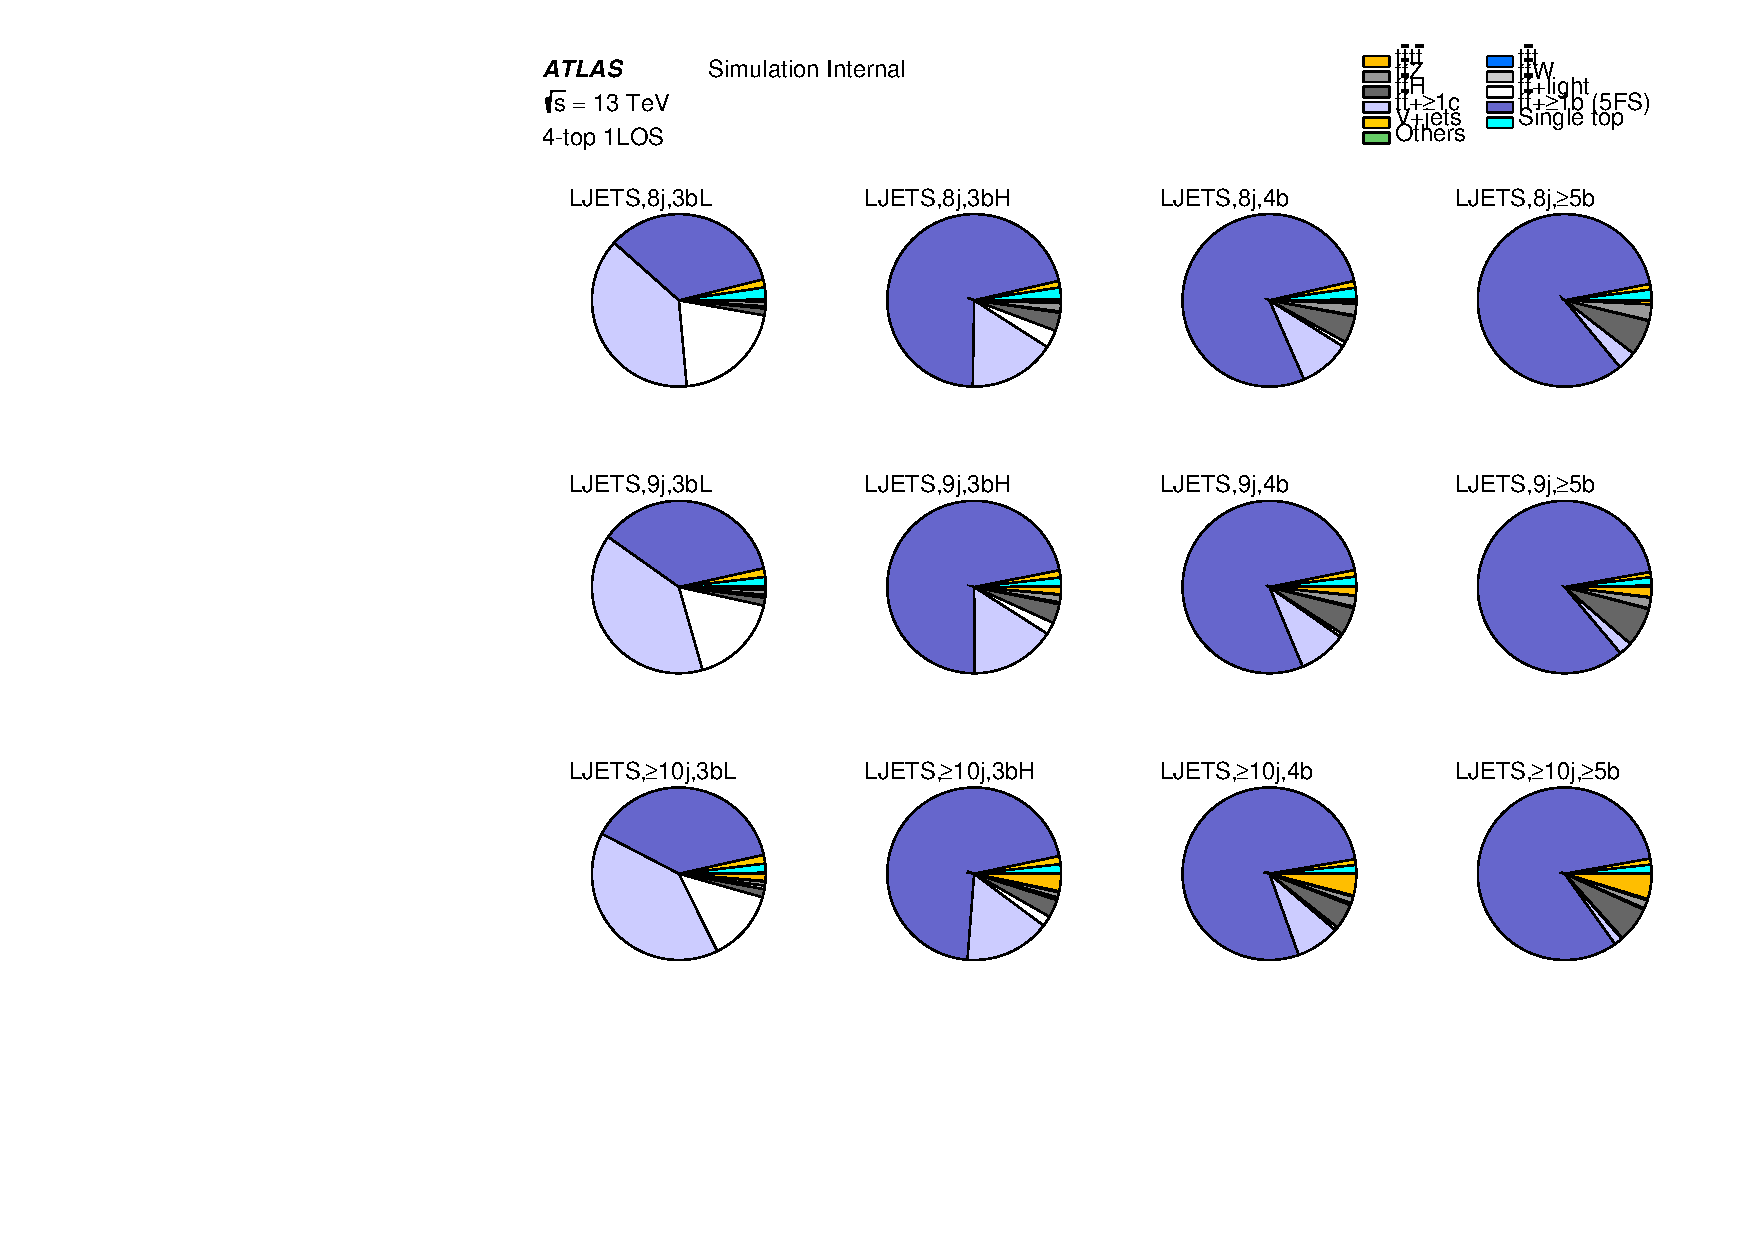
\includegraphics[width=0.48\textwidth]{figures/piechart/PieChart_1l.pdf}
          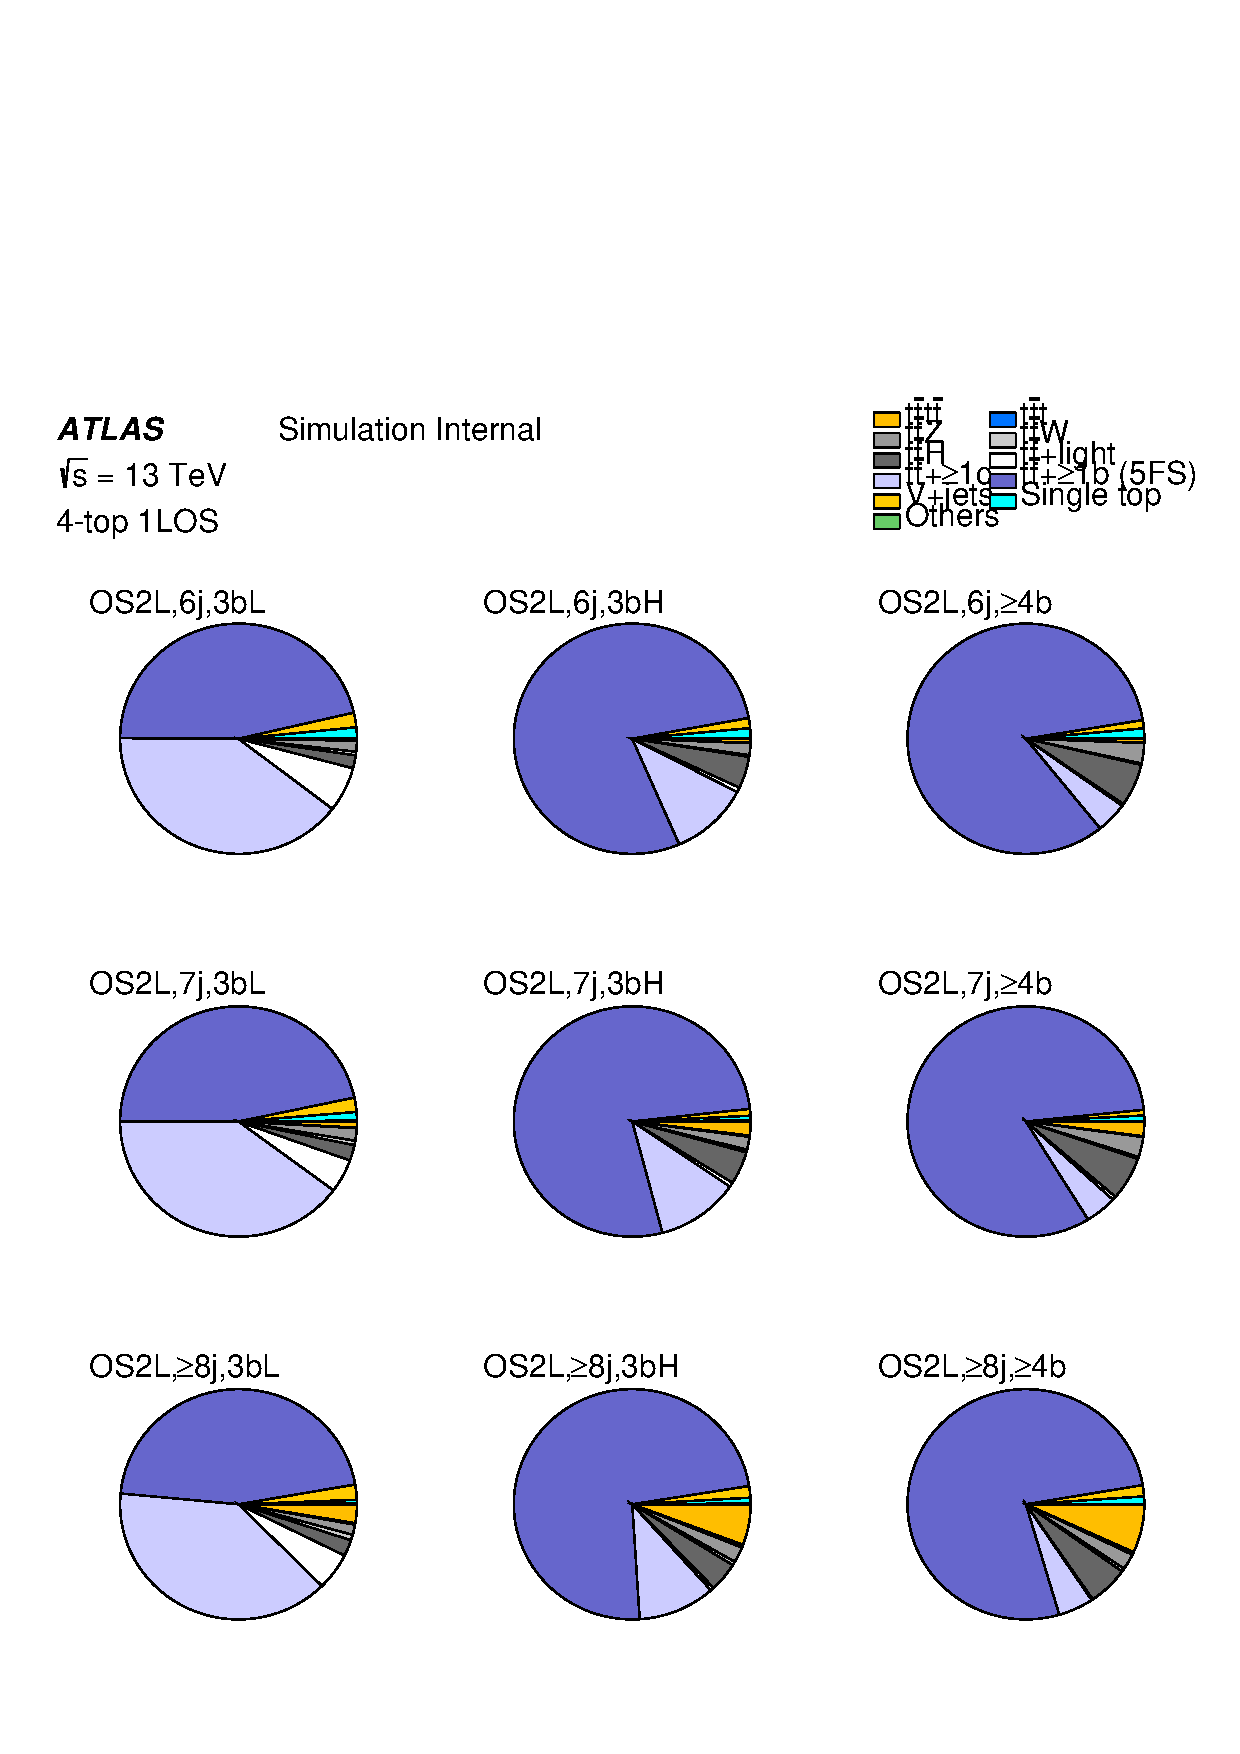
\includegraphics[width=0.48\textwidth]{figures/piechart/PieChart_2l.pdf}
      \end{subfigure}
      \caption{Pie charts of the selected region for 1L (left), and 2LOS (right).}
      \label{fig::piechart}
  \end{figure}


%-------------------------------------------------------------------------------                


%-------------------------------------------------------------------------------                                                                                                
\FloatBarrier
\section{Analysis strategy}% Daniela, Nicola
\label{sec:strategy}
After the event selection (see Section~\ref{sec:event_selection}) the events are categorised based on the lepton multiplicity (1L or 2LOS), jets multiplicity and b-jets multiplicity. The two leptonic channels are analysed separately and combined only for the final results. 
In the 1L (2LOS) channel, events are retained for the final analysis if they contain at least 7 (5) jets and at least two $b$-tagged jets (a jet is considered as $b$-tagged if it passes an OP of 70\% efficiency). 
Signal-depleted and signal-rich analysis regions are defined from different combinations of jets and $b$-jets multiplicity requirements.  
An illustration of the used analysis regions is given in Figure~\ref{fig:regions}. The $b$-jets multiplicity requirements combine multiple $b$-tagging OP as described in Table~\ref{tab:regions}. The b-tagged jets are counted across different OPs using \textbf{AND} logic. The events in each category must fulfil all the three b-jets multiplicity requirements simultaneously. For example, in 3bH selection, an event should contain exactly three b-tagged jets obtained using b-tagging OPs with an average expected efficiencies of 60\%, exactly three b-tagged jets obtained using b-tagging OPs with an average expected efficiencies of 70\% and more than three b-tagged jets obtained using b-tagging OPs with an average expected efficiencies of 85\%.

\begin{table}[!hbt]
  \begin{center}
    \caption{
      Summary of the $b$-tagging requirements for the event categorisation.
      Events in each category must satisfy all requirements listed in columns.
      $N_b^{60\%}$, $N_b^{70\%}$ and $N_b^{85\%}$ are defined as the numbers of $b$-tagged jets
      obtained using $b$-tagging operating points with average
      expected efficiencies of 60\%, 70\% and 85\%, respectively.
      The 3bL (3bH) requirement selects events with lower (higher) purity of
      MC `truth' $b$-jets amongst the three jets tagged at the 70\% OP.
      The 3bV requirement is used to define the validation regions.
      The symbol `-' indicates that no requirement is applied.
      \newline
    }
    \begin{tabular}{m{6em}m{5em}m{5em}m{5em}}
      \hline
      \\[-1em]
      Name & $N_b^{60\%}$ &  $N_b^{70\%}$ & $N_b^{85\%}$ \\
      \\[-1em]
      \hline
      2b             & -       & = 2     & - \\
      3bL            & $\le$ 2 & = 3     & - \\
      3bH            & = 3     & = 3     & > 3 \\
      3bV            & = 3     & = 3     & = 3 \\
      $\ge$4b (2LOS) & -       & $\ge$ 4 & - \\
      4b (1L)        & -       & = 4     & - \\
      $\ge$5b (1L)   & -       & $\ge$ 5 & - \\
      \hline
    \end{tabular}
    \label{tab:regions}
  \end{center}
\end{table}

\begin{figure}[tbp]
  \begin{center} \setlength{\tabcolsep}{7.5pt}\footnotesize
    \begin{tabular}{cc}
        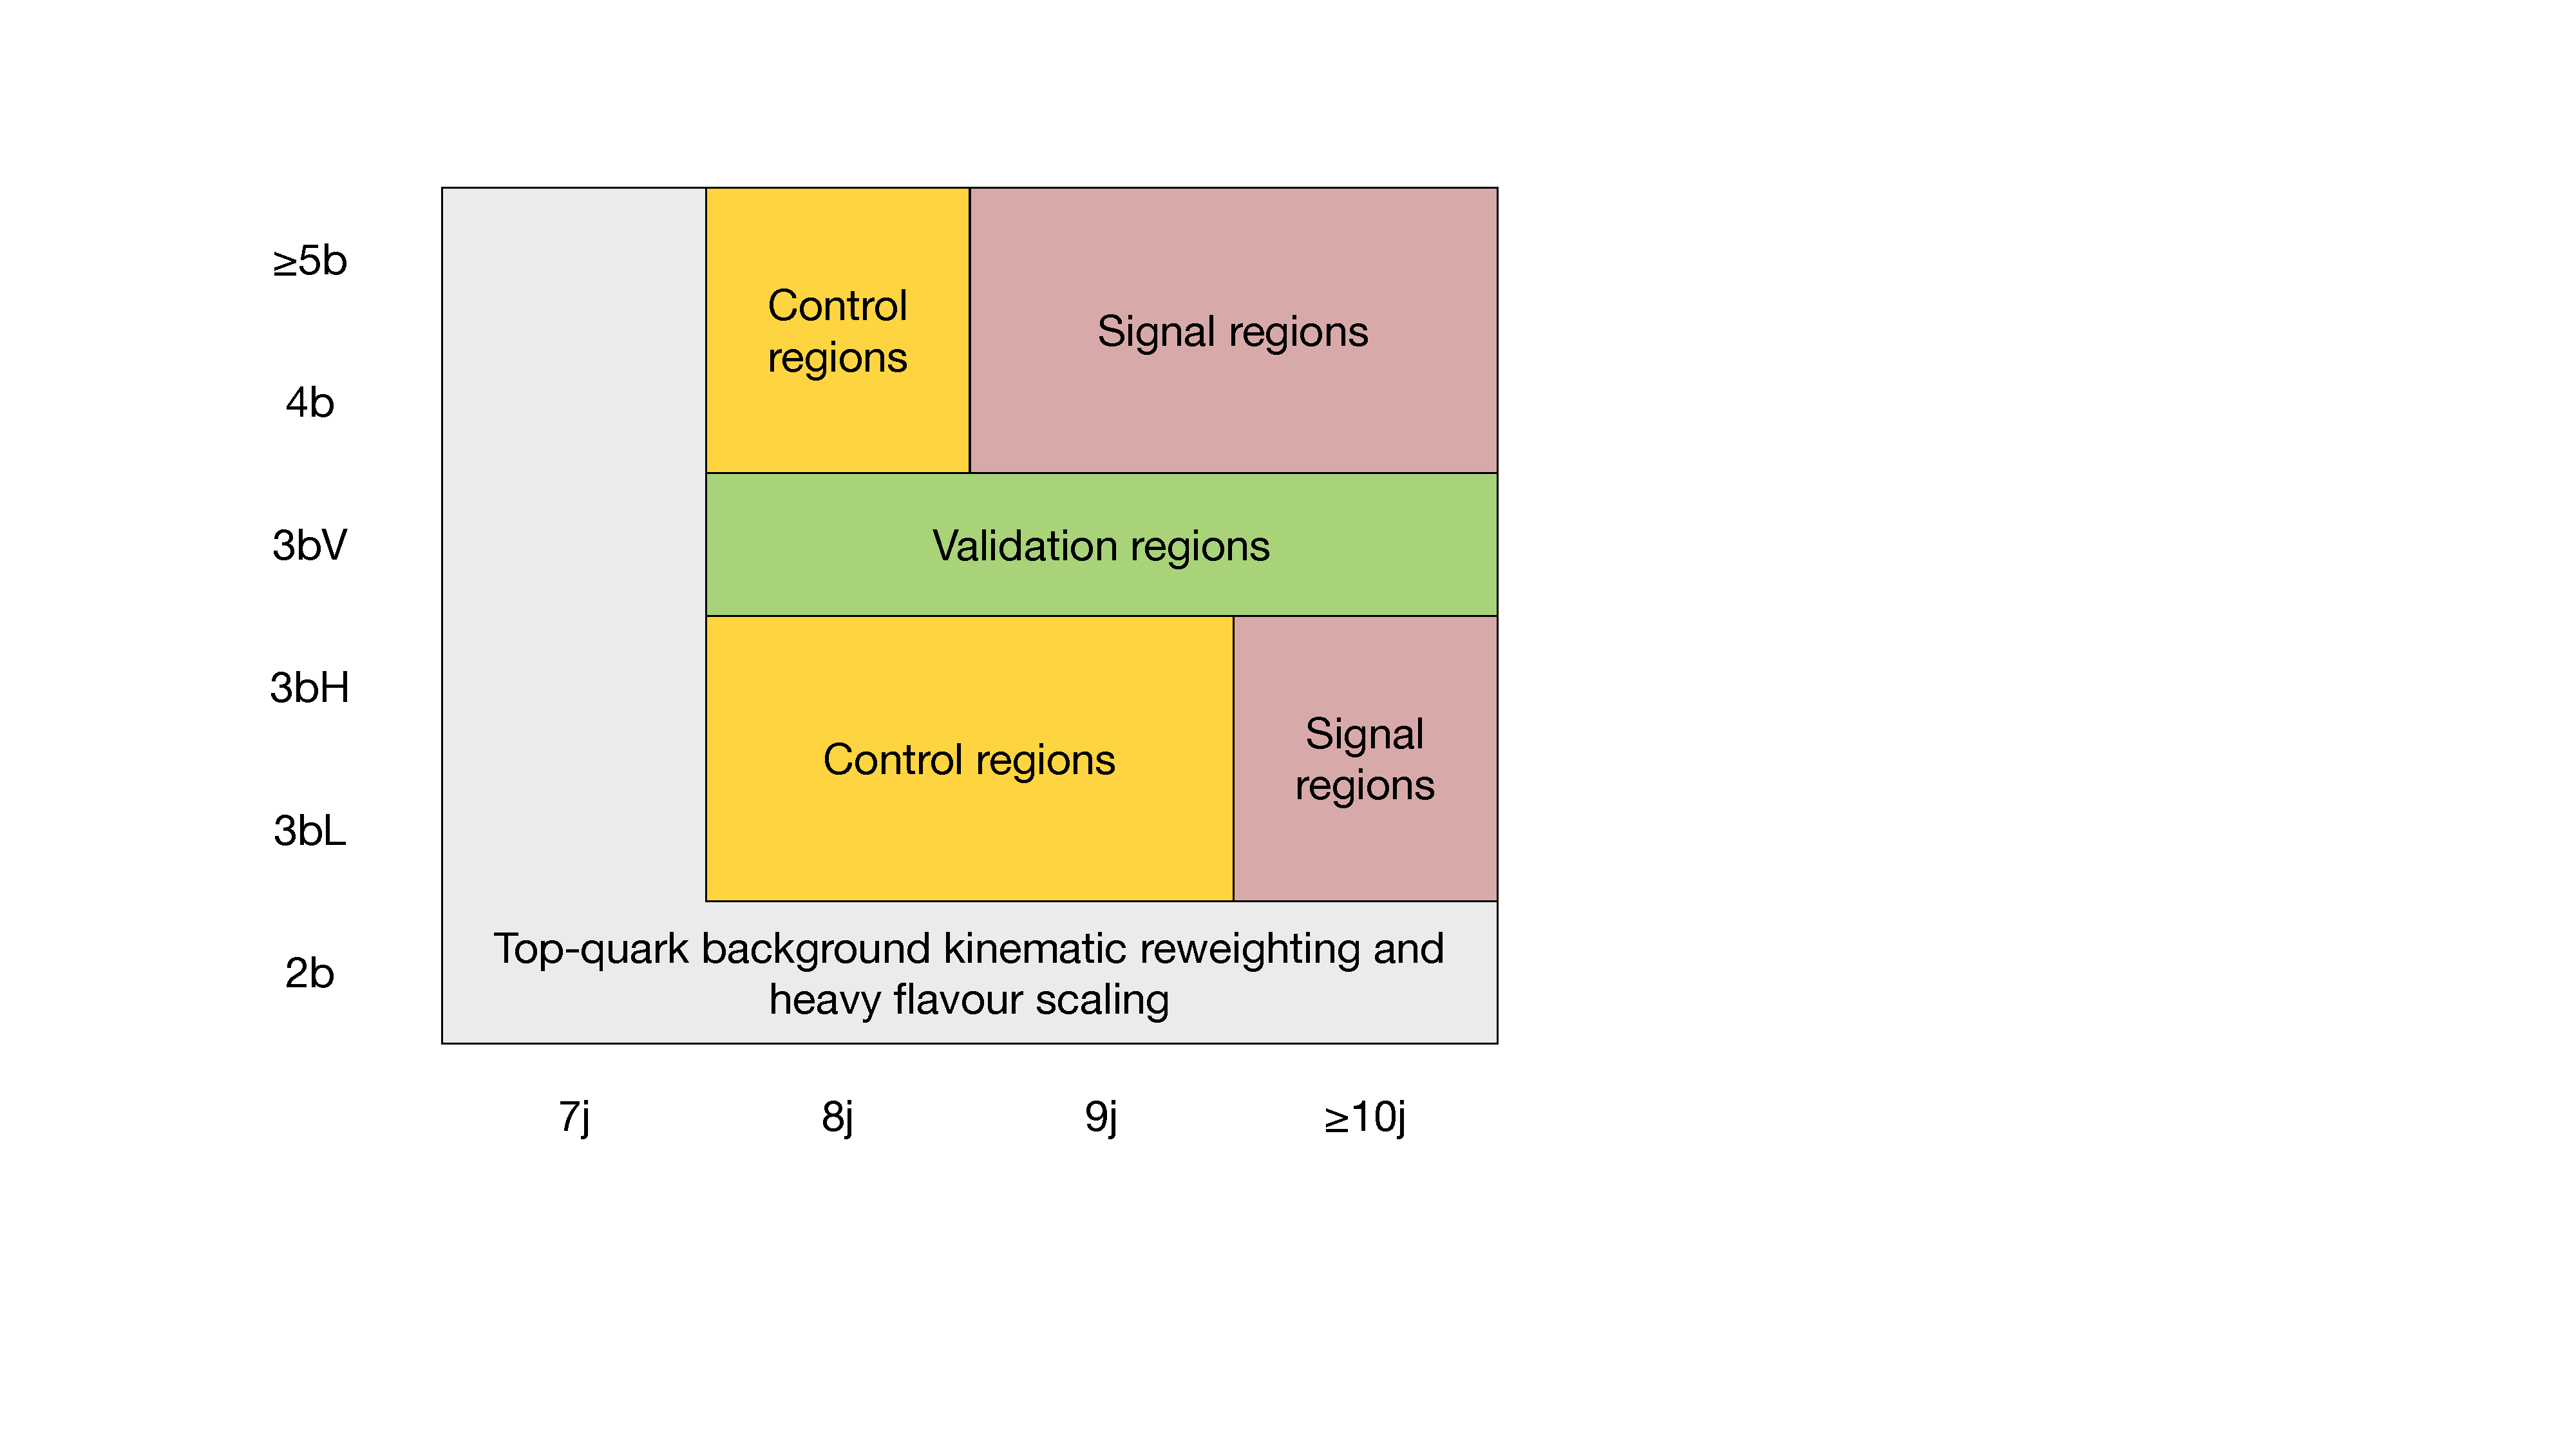
\includegraphics[width=0.46\textwidth]{figures/strategy/1l_regions} &
        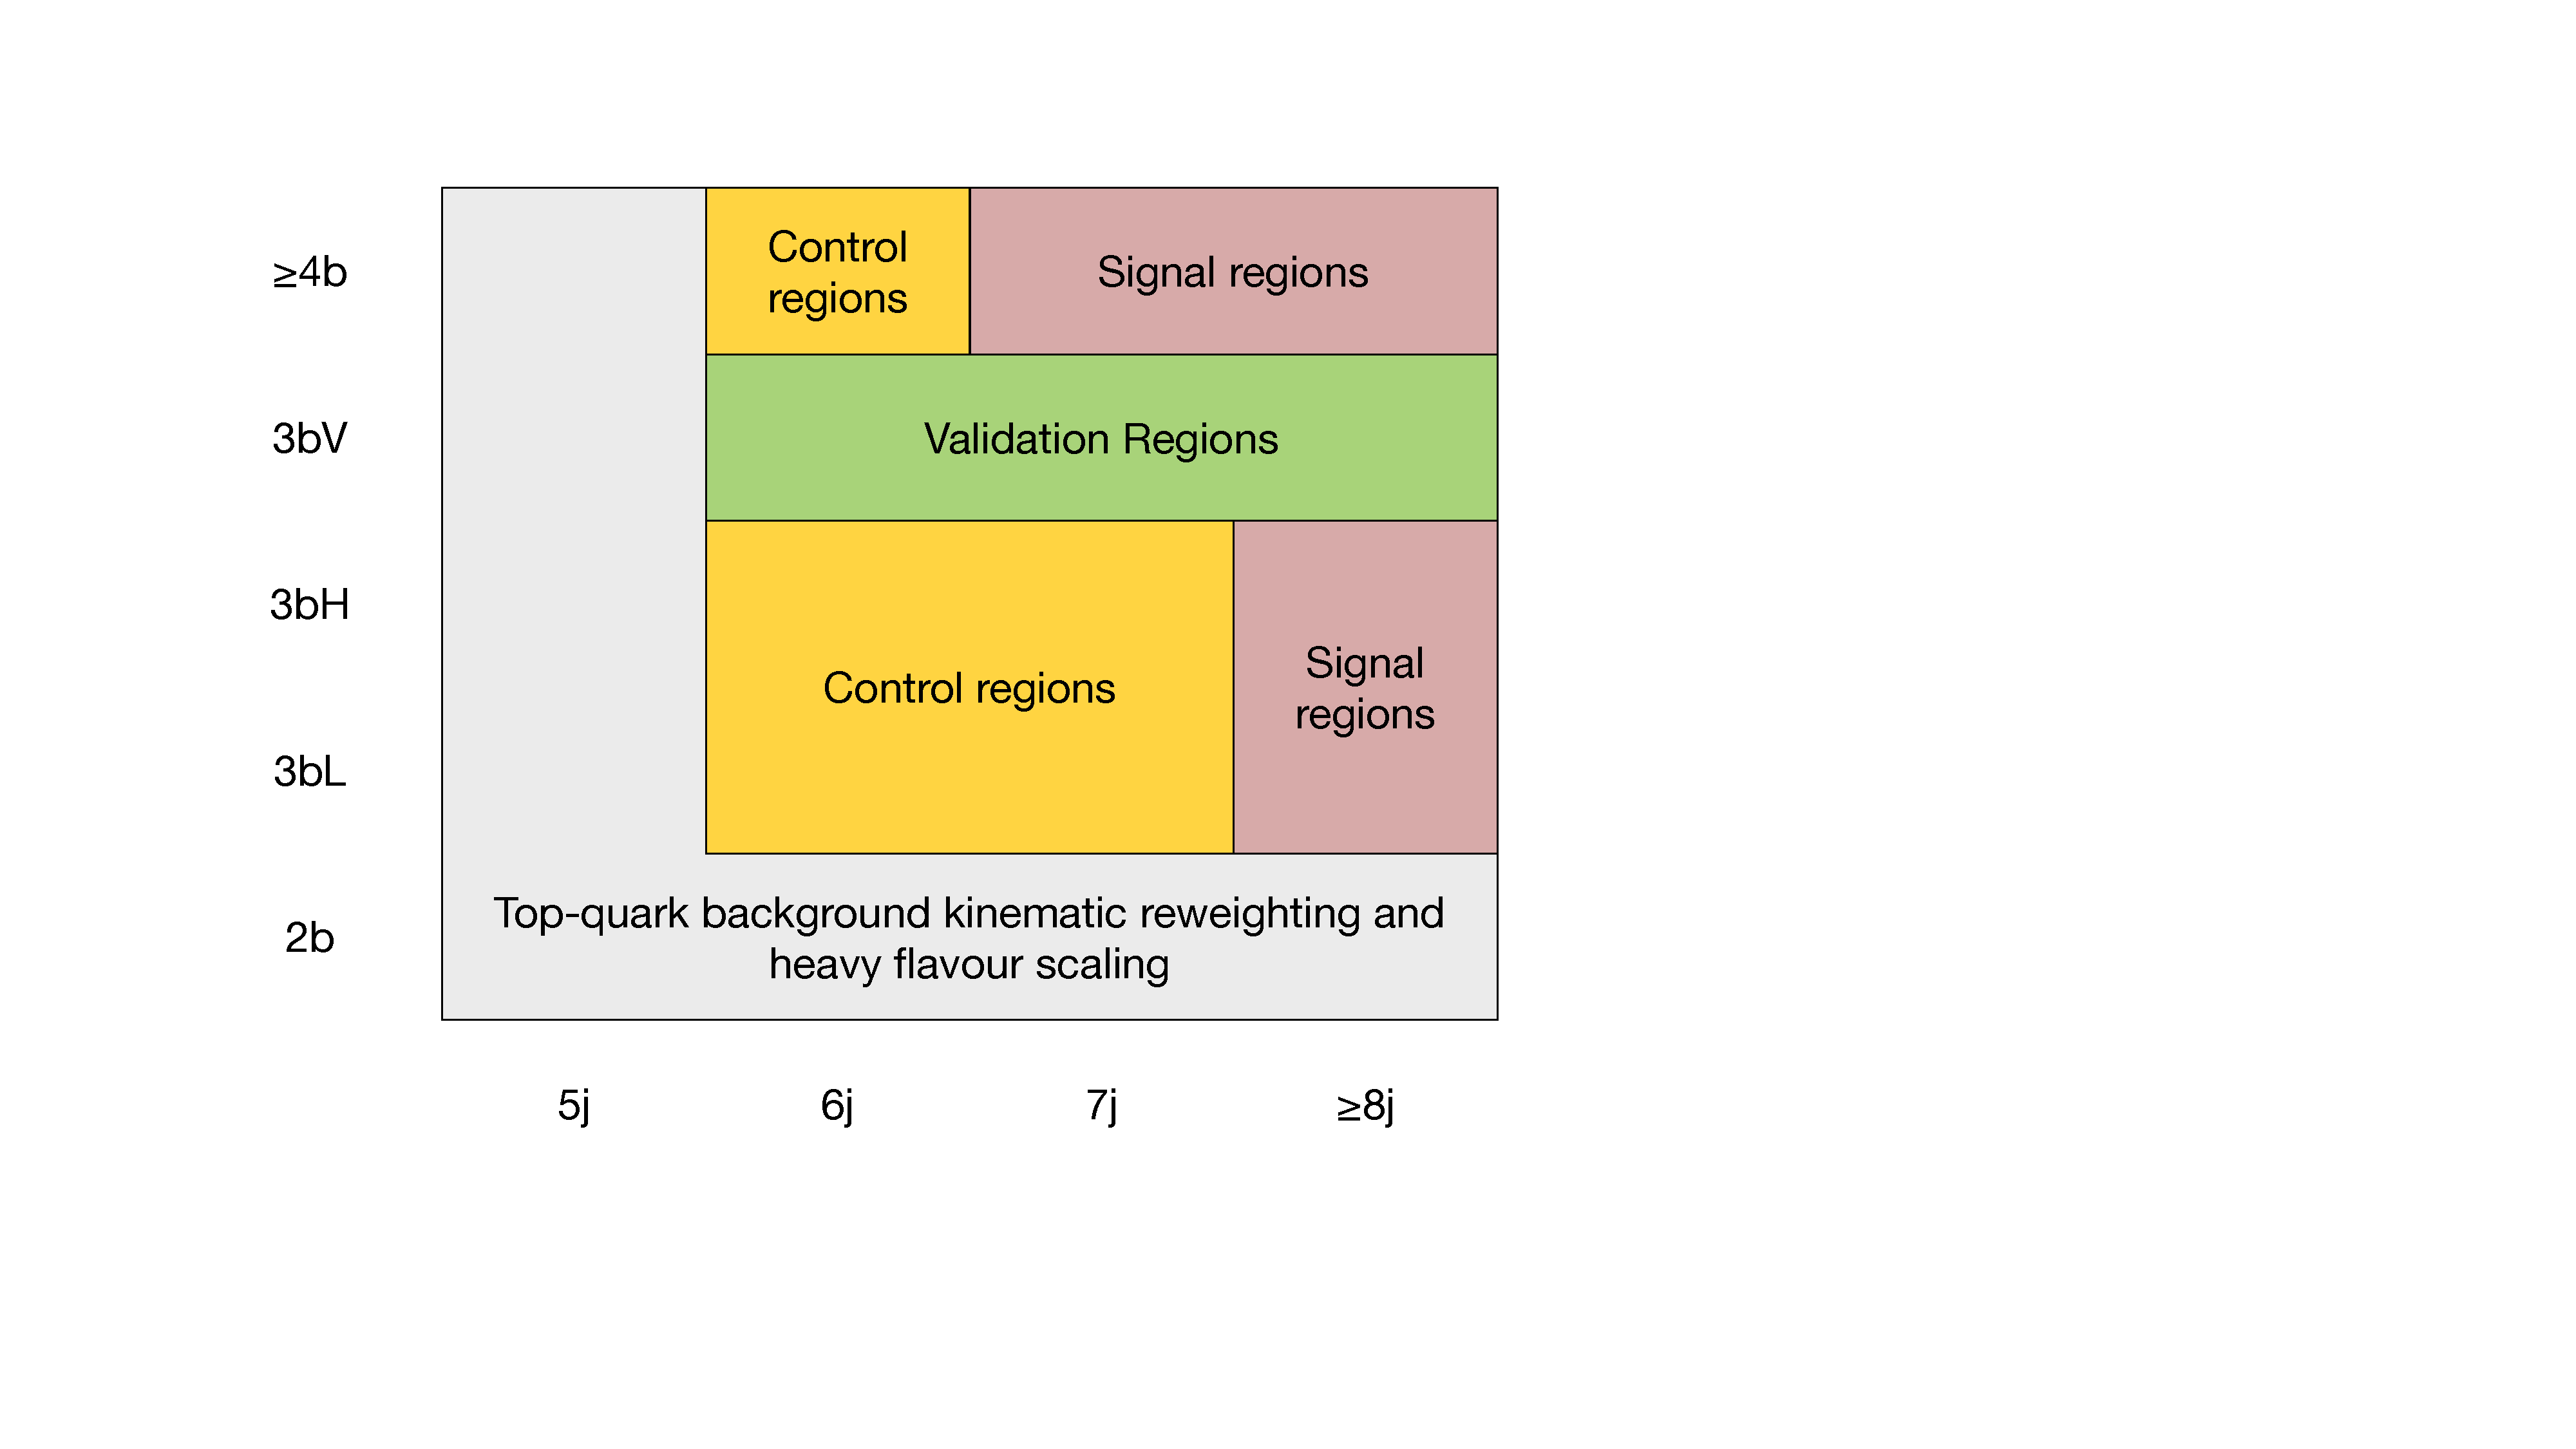
\includegraphics[width=0.46\textwidth]{figures/strategy/2los_regions} \\
        (1L) & (2LOS) \\
    \end{tabular}
     \caption{Schematic view of the event categories used to select analysis regions (signal, control, validation and $\ttbar$+jets reweighting regions) in the 1L channel (left) and 2LOS channel (right). The axes represent the jet multiplicity and $b$-tagging requirements defined in Table~\ref{tab:regions}. The 3bL (3bH) $b$-tagging requirement selects events with lower (higher) purity of MC 'truth' $b$-jets amongst the three jets tagged at the 70\% OP. The 3bV $b$-tagging requirement is used to define the validation regions.}
   \label{fig:regions}
  \end{center}
\end{figure}

The SM background is estimated by using samples of simulated events as described in Section~\ref{sec:samples}. 
The main background originates from $\ttbar$+jets production.  As discussed in Section~\ref{sec:nn_rew}, a reweighting procedure is implemented to adjust the MC modelling  of $\ttbar$+jets production based on a  combined use of events with low jet multiplicity and large b-jets multiplicity as well as events with large jet multiplicity and low b-jets multiplicity after checking that the signal contamination in those regions is negligible. The regions used to derive the reweighting for the $\ttbar$+jets background are highlighted in grey colour in Figure~\ref{fig:regions}. 

A potential BSM signal is identified by using MVA discriminants. As described in Section~\ref{sec:mva} two MVA discriminants are developed, are used throughout the analysis and facilitate their mutual validation by extensive fit studies and modelling studies in signal-depleted regions.    
The MVA and H$_T$ distributions from each of the regions with at least 3 $b$-jets are simultaneously used to test for the presence of a signal. 
A total of 21 regions are used in the profile likelihood fit, with 12 regions in the 1L channel and
9 regions in the 2LOS channel.
They are defined by considering the regions with at least 8 (6) jets in the 1L (2LOS) channel and
satisfying the 3bL, 3bH or $\ge$4b requirements.
Among these regions, the ones that have at least 10 (8) jets or have 9 (7) jets and satisfy the $\ge$4b
requirement in the 1L (2LOS) channel are defined as the signal regions.
The rest of the fitted regions are defined as the control regions.
A total of 6 validation regions are also defined by considering the regions with at least 8 (6)
jets in the 1L (2LOS) channel and satisfying the 3bV requirement.
The validation regions are not used in the fit and hence do not contribute to the signal extraction.
The variables and binning used in each region is optimised as discussed in Sec.~\ref{sec:binning}. 

%-------------------------------------------------------------------------------     


%-------------------------------------------------------------------------------                                                                                                
\FloatBarrier
\section{\ttbar\ background estimation}% Anil
\label{sec:ttbar_rew}
The Monte Carlo (MC) prediction of the nominal \ttbar + jets production samples (Powheg+Pythia8) up to six additional jets is not fully reliable. Therefore, data-based corrections, derived and applied before the fit to extract the signal, are a key ingredient in this analysis.

The two sources of mismodelling individually corrected by using data-driven correction factors. First, the rate of the \ttbar production in association with heavy-flavor jets (referred to as \ttbar +HF) is under-estimated, as observed by several previous searches and measurements. This is corrected by rescaling the normalization of each \ttbar +jets category based on the flavor of the extra jets, by comparing the yields of the data and the MC prediction in regions with different $b$-tagging requirements.

The jet multiplicity and the kinematic features of the additional jets are known to be mismodelled by the MC predictions at  multiplicity. A correction is then deployed by applying reweighting factors on the mismodelled observables, derived by comparing their distributions between the data and the MC prediction in the 2b region.
In this second step, a neural network-based approach is used to estimate the probability density functions of the data and the MC prediction, to derive reweighting factor as a ratio of them. This method allows to correct multiple observables at the same time, thus the MVA strategy used to define a signal-to-background discriminant has further flexibility on the input features choice as their modelling will typically be corrected.

%\subsection{\ttbar + jets truth classification}

\subsection{Flavor rescaling}
\label{sec:hf_rew}
The flavor rescaling corrects the under-estimation of the $\ttbar+HF$ production rate in the MC prediction. This is performed by rescaling the normalization of $\ttbar+light$ (TTL), $\ttbar+\ge 1c$ (TTC) and $\ttbar+\ge 1b$ (TTB). The scale factors are derived by performing a likelihood fit on the sum of the pseudo continuous b-tagged score (pcb) of the third and forth jets ranked in DL1r score, as this variable is highly sensitive to the $\ttbar+HF$ samples. A combined fit is performed in 7j region from the 1L channel and 5j region from the OS channel with $=2b$, $=3b$ and $\geq 4b$ requirements, where the signal contamination of all the signal mass points is around or smaller than $0.1\%$. The normalisation of TTL, TTC and TTB are free floating in this fit, and that TTL normalisation for 1L and 2LOS are treated as two independent normalisaiton factors. The nominal \ttbar sample is used for this fit. The nuisance parameters associated to the systematic uncertainties on the b-tagging efficiency (as described in Section~\ref{b-tagging_uncertianties}) and the cross-section uncertainties of other backgrounds, which cannot be neglected in the fitting regions, are fitted together with the correction factors of TTL, TTC and TTB because these uncertainties highly affect the yields of $\ttbar+HF$ and other backgrounds.

% as given in the Table~\ref{tab:HF_postFit_nominal}

\begin{table}[th!]
    \centering
    \def\arraystretch{1.2}
    \resizebox*{0.3\textwidth}{!}{
    \begin{tabular}{c|cc}
        \toprule
          & 1L & OS \\
          & $=7j$ & $=5j$ \\
        \hline
         2b & $<0.1\%$ & $<0.1\%$ \\
         3b & $<0.1\%$ & $<0.1\%$ \\
         $\geq4b$ & $0.2\%$ & $0.1\%$ \\
        \bottomrule
    \end{tabular}
    }
    \caption{\label{tab:sigContam_HFCorrRegion}The signal (BSMtttt M700) over background ratio in each of the regions used to derive the HF rescaling factors before any scaling applied.}
\end{table}

The pre-fit and post-fit distributions of the third and the forth jets pcb sum in 1L and OS channels can be found in figure~\ref{fig:1L_pcb34_PrePost} and~\ref{fig:2LOS_pcb34_PrePost} respectively. The pre-fit and post-fit summary plots, which show the yields in each region, in both channel can be found in figure~\ref{fig:HF_summaryPlot} while the fitted normalization factors and nuisance parameters can be found in figure~\ref{fig:HF_scale_fit}. The obtained normalization factors are consistent with other ATLAS analyses targeting similar phase space. For example, the ttH(bb) measurement \cite{HIGG-2017-03} found tt+b and tt+c normalization factors of 1.24 and 1.63, respectively. Most of the nuisance parametrs are neither pulled nor constrained. However, when the fits are done separately on two channels, it is observed that both nuisance parameters of c-tagging EV0 and light-tagging EV0 are pulled in oposite direction between two channels. Therefore these two nuisance parameters are decorrelated from the two channels in the combined fit.
It is also found that having the combined fit in TTL scale factor causes the inconsistent results with the 1L and OS channel separated fit, because the acceptance of the TTL events between these two channel are different. To keep a stable fit results, the TTL correction factors are derived on separate channels during the combined fit.



\begin{figure}[!htb]
    \centering
    \subfloat[1L$(=7j,=2b)$ Pre-fit]{
        
\includegraphics[height=0.3\textheight]{plots/bkg_modelling/HF_scaling/pcbSum34_ljets_7j2b_preFit.pdf}
    }
    \subfloat[1L$(=7j,=2b)$ Post-Fit]{
        
\includegraphics[height=0.3\textheight]{plots/bkg_modelling/HF_scaling/pcbSum34_ljets_7j2b_postFit.pdf}
    }

    \subfloat[1L$(=7j,=3b)$ Pre-fit]{
        
\includegraphics[height=0.3\textheight]{plots/bkg_modelling/HF_scaling/pcbSum34_ljets_7j3b_preFit.pdf}
    }
    \subfloat[1L$(=7j,=3b)$ Post-Fit]{
        
\includegraphics[height=0.3\textheight]{plots/bkg_modelling/HF_scaling/pcbSum34_ljets_7j3b_postFit.pdf}
    }
    
    \subfloat[1L$(=7j,\geq 4b)$ Pre-fit]{
        
\includegraphics[height=0.3\textheight]{plots/bkg_modelling/HF_scaling/pcbSum34_ljets_7jge4b_preFit.pdf}
    }
    \subfloat[1L$(=7j,\geq 4b)$ Post-Fit]{
        
\includegraphics[height=0.3\textheight]{plots/bkg_modelling/HF_scaling/pcbSum34_ljets_7jge4b_postFit.pdf}
    }
    \caption{\label{fig:1L_pcb34_PrePost}The pre-fit (left) and post-fit (right) distributions of pcb sum of the third and the forth jets at 7j region with $=2b$, $=3b$ and $\geq 4b$ in 1L channel to derive the HF scale factor.}
\end{figure}


\begin{figure}[!htb]
    \centering
    \subfloat[1L$(=5j,=2b)$ Pre-fit]{
        
\includegraphics[height=0.3\textheight]{plots/bkg_modelling/HF_scaling/pcbSum34_os2l_5j2b_preFit.pdf}
    }
    \subfloat[1L$(=5j,=2b)$ Post-Fit]{
        
\includegraphics[height=0.3\textheight]{plots/bkg_modelling/HF_scaling/pcbSum34_os2l_5j2b_postFit.pdf}
    }

    \subfloat[1L$(=5j,=3b)$ Pre-fit]{
        
\includegraphics[height=0.3\textheight]{plots/bkg_modelling/HF_scaling/pcbSum34_os2l_5j3b_preFit.pdf}
    }
    \subfloat[1L$(=5j,=3b)$ Post-Fit]{
        
\includegraphics[height=0.3\textheight]{plots/bkg_modelling/HF_scaling/pcbSum34_os2l_5j3b_postFit.pdf}
    }

    \subfloat[1L$(=5j,\geq 4b)$ Pre-fit]{
        
\includegraphics[height=0.3\textheight]{plots/bkg_modelling/HF_scaling/pcbSum34_os2l_5jge4b_preFit.pdf}
    }
    \subfloat[1L$(=5j,\geq 4b)$ Post-Fit]{
        
\includegraphics[height=0.3\textheight]{plots/bkg_modelling/HF_scaling/pcbSum34_os2l_5jge4b_postFit.pdf}
    }
    \caption{\label{fig:2LOS_pcb34_PrePost}The pre-fit (left) and post-fit (right) distributions of pcb sum of the third and the forth jets at 5j region with $=2b$, $=3b$ and $\geq 4b$ in OS channel to derive the HF scale factor.}
\end{figure}

\begin{figure}[ht!]
  \centering
    \begin{subfigure}[t]{\textwidth}
        \centering
        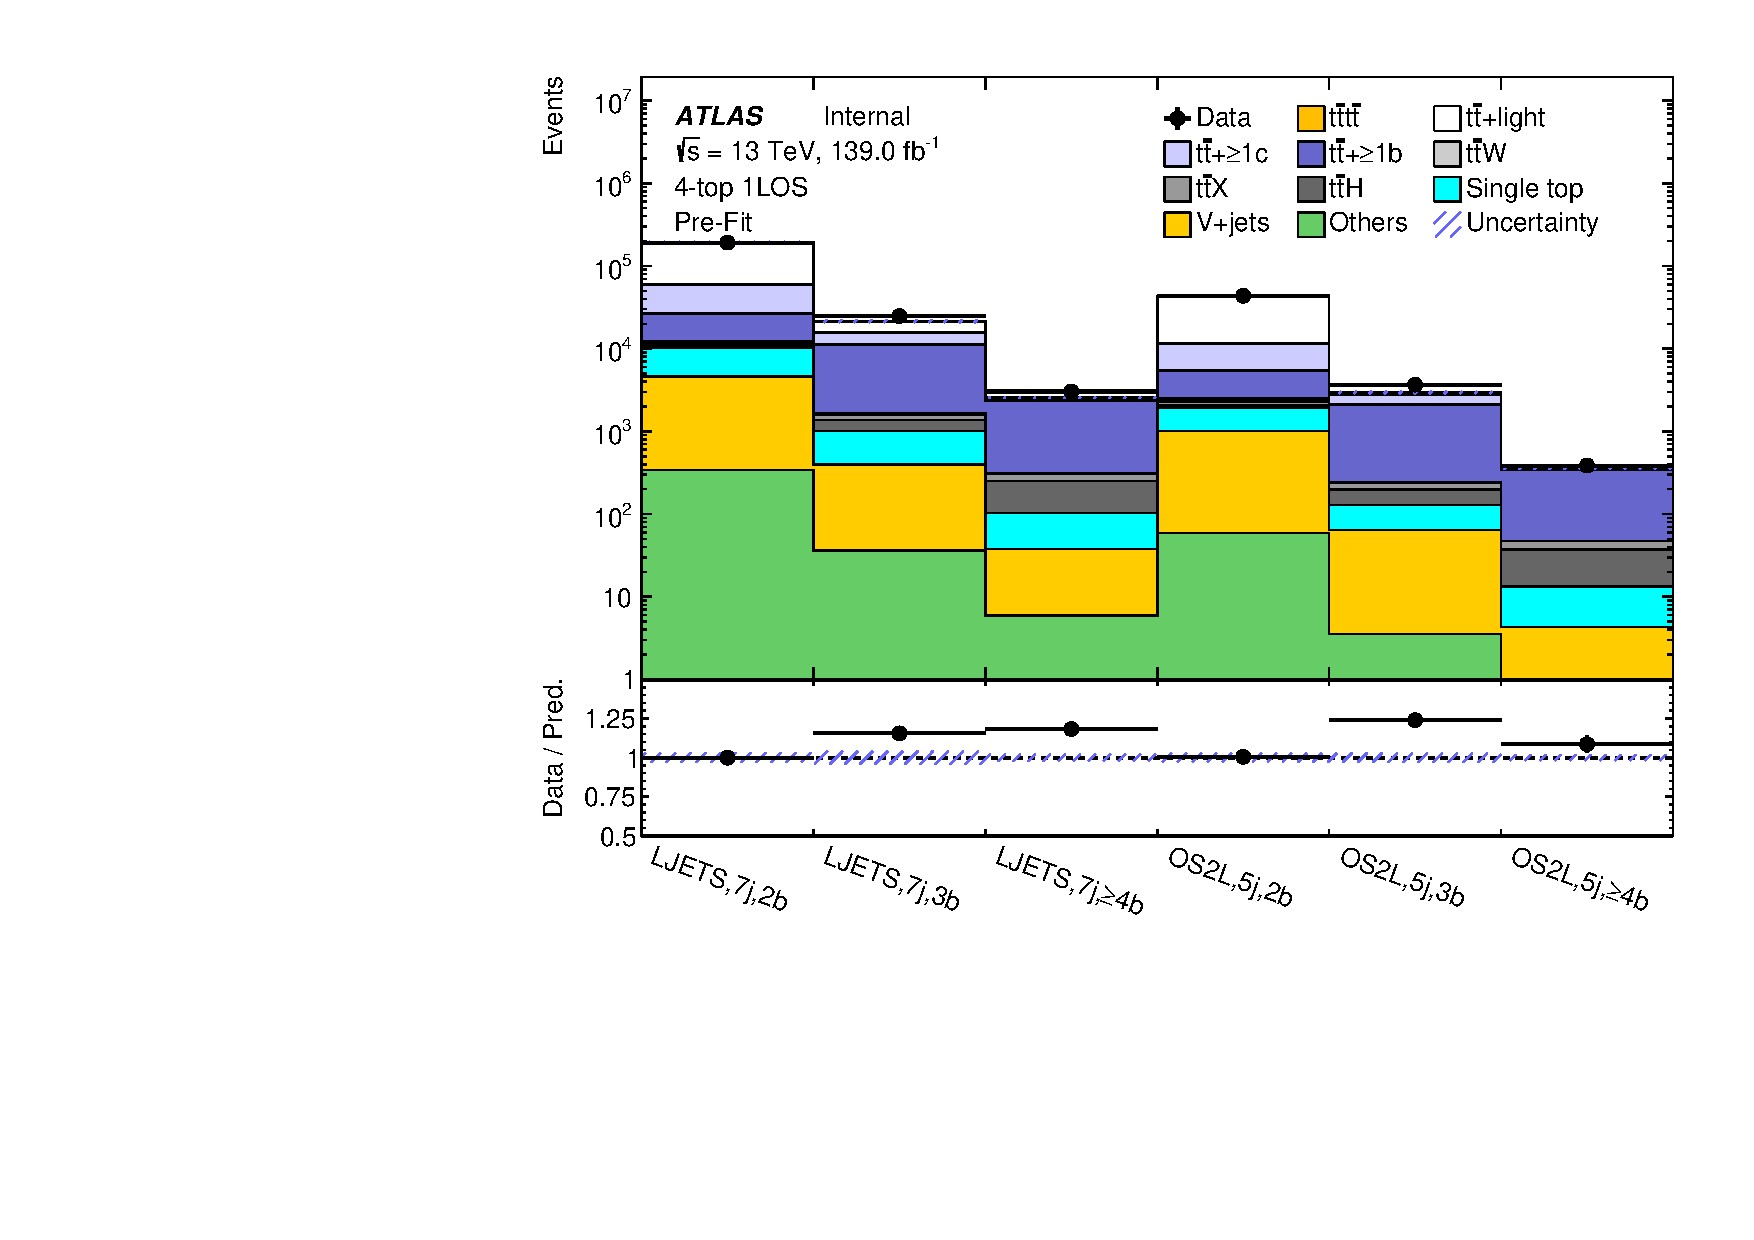
\includegraphics[width=0.48\textwidth]{plots/bkg_modelling/HF_scaling/Summary_preFit.pdf}
        
\includegraphics[width=0.48\textwidth]{plots/bkg_modelling/HF_scaling/Summary_postFit.pdf}
    \end{subfigure}
    \caption{Pre-fit (left) and post-fit (right) distributions of the yields in the regions included in the fit to determine HF scale factors.}
    \label{fig:HF_summaryPlot}
\end{figure}

\begin{figure}[ht!]
  \centering
    \begin{subfigure}[t]{\textwidth}
        \centering
        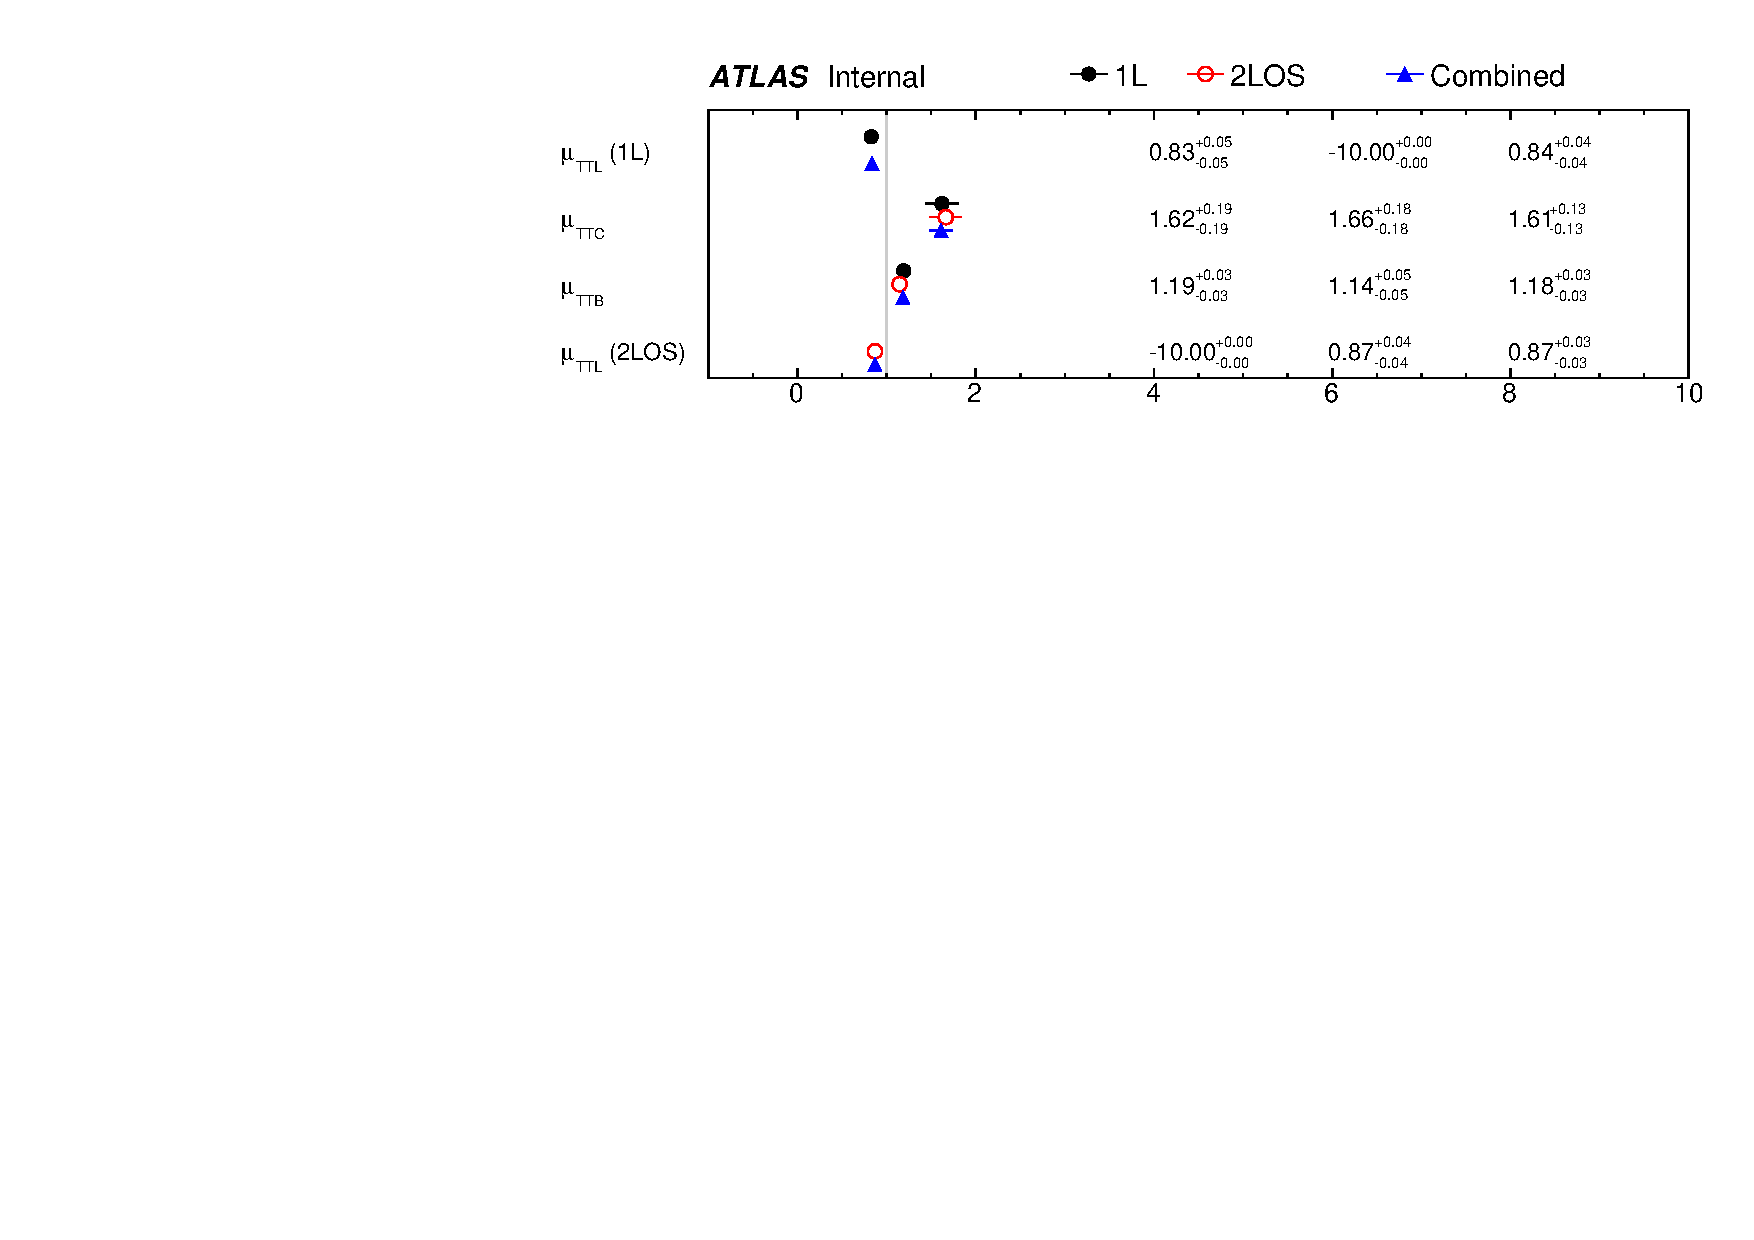
\includegraphics[width=0.78\textwidth]{plots/bkg_modelling/HF_scaling/NormFactors_multiFit.pdf}
    \end{subfigure}
    \bigskip
    \centering
    \begin{subfigure}[t]{\textwidth}
        \centering
        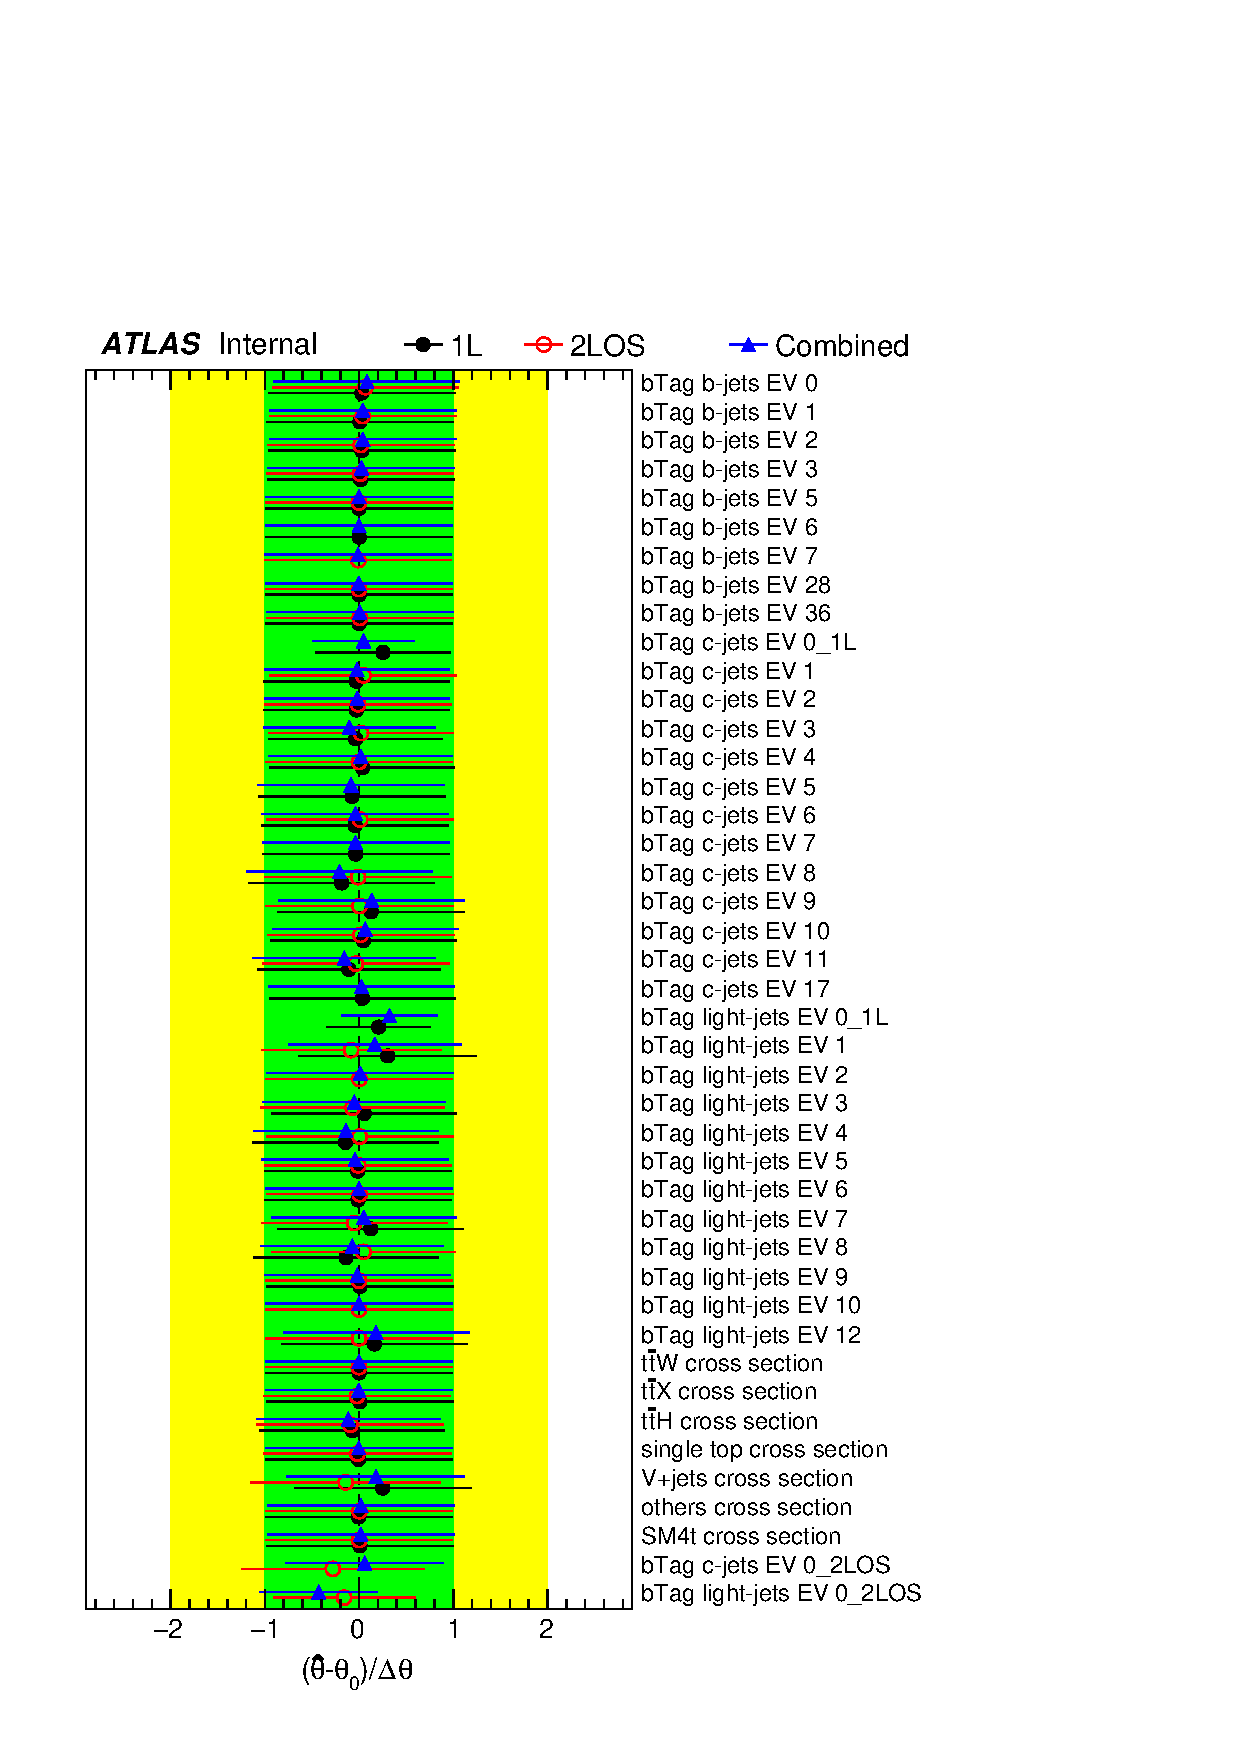
\includegraphics[width=0.58\textwidth]{plots/bkg_modelling/HF_scaling/PullPlots_multiFit.pdf}
    \end{subfigure}
    \caption{Fitted normalisation factors and nuisance parameters. Black, red and blue color refer to 1L, OS and combined channel fit respectively.}
    \label{fig:HF_scale_fit}
\end{figure}



The HF scale factors used in this analysis for the nominal \ttbar sample are taken as the normalization factors from Figure \ref{fig:HF_scale_fit}. It was found that the ratio $\ttbar_{postfit}^{nominal} / \ttbar_{prefit}^{nominal}$ based on Tables~\ref{tab:HF_preFit} and \ref{tab:HF_postFit_nominal} is very similar to the obtained normalization factors (1.18 for \ttbin, 1.60 for \ttcin, 0.83 for TTL (1L), and  0.87 for TTL (2L)).

The HF scale factors for the alternative \ttbar\ samples are obtained as the ratio $\ttbar_{postfit}^{nominal} / \ttbar_{prefit}^{alternative}$ based on the Tables~\ref{tab:HF_preFit} and \ref{tab:HF_postFit_nominal}. This is the preferred option because it also contains effects from the pulls from all nuisance parameters (it makes no difference for the nominal sample). No separate fits with alternative samples were used because they lead to large pulls on several nuisance parameters.  The HF scale factors of different \ttbar samples are summarized in table~\ref{tab:HF_results}. The \ttbar modelling systematics obtained using alternative weights in the nominal \ttbar sample (FSR, ISR, renormalization and factorization scale) are using the HF scale factors for the nominal \ttbar sample (the differences are negligible as documented in Appendix \ref{app:HFweights_weightSystematics}).


\begin{table}[!htb]
    \centering
    \resizebox*{0.72\textwidth}{!}{
    \begin{tabular}{c|c|c|c||c}
        \hline \hline
        \multicolumn{5}{c}{\textbf{Pre-fit 1L (Nominal)}}\\
        \hline
        & $LJETS,7j,2b$ & $LJETS,7j,3b$ & $LJETS,7j,\geq 4b$ & Total \\
        \hline 
TTL &  $132532.64 \pm 4215.99 $ & $5751.48 \pm 470.26$ & $44.24 \pm 11.26$ & $138328.36 \pm 4242.15$\\
TTC & $32634.67 \pm 888.81$ & $4491.35 \pm 360.70$ & $181.26 \pm 27.45$ & $37307.28 \pm 959.60$ \\
TTB & $14525.10 \pm 17.06$ & $9577.63 \pm 12.25$ & $2016.50 \pm 4.30$ & $26119.23 \pm 21.44$ \\ 
        \hline \hline
        \multicolumn{5}{c}{\textbf{Pre-fit OS (Nominal)}}\\
        \hline
        & $OS2L,5j,2b$ & $OS2L,5j,3b$ & $OS2L,5j,\geq 4b$ & Total \\
        \hline 
TTL &  $31869.24 \pm 961.92$ & $189.42 \pm 38.91$ & $0.51 \pm 0.26$ & $32059.17 \pm 962.71$\\
TTC & $6015.13\pm 150.02$ & $645.69 \pm 52.96$ & $10.95 \pm 1.71$ & $6671.77 \pm 159.10$  \\
TTB & $2994.50 \pm 5.91$ & $1870.36 \pm 4.24$ & $296.20 \pm 1.36$ & $5161.06 \pm 7.40$ \\
        \hline \hline \hline
        \multicolumn{5}{c}{\textbf{Pre-fit 1L (ttbb 4FS)}}\\
        \hline
        & $LJETS,7j,2b$ & $LJETS,7j,3b$ & $LJETS,7j,\geq 4b$ & Total \\
        \hline
TTL &  $132532.64 \pm 4215.99 $ & $5751.48 \pm 470.26$ & $44.24 \pm 11.26$ & $138328.36 \pm 4242.15$\\
TTC & $32634.67 \pm 888.81$ & $4491.35 \pm 360.70$ & $181.26 \pm 27.45$ & $37307.28 \pm 959.60$ \\
TTB & $14395.47 \pm 27.52$ & $9852.50 \pm 22.34$ & $2180.87 \pm 10.15$ & $26428.84 \pm 36.87$ \\
        \hline \hline
        \multicolumn{5}{c}{\textbf{Pre-fit OS (ttbb 4FS)}}\\
        \hline
         & $OS2L,5j,2b$ & $OS2L,5j,3b$ & $OS2L,5j,\geq 4b$ & Total \\
        \hline
TTL &  $31869.24 \pm 961.92$ & $189.42 \pm 38.91$ & $0.51 \pm 0.26$ & $32059.17 \pm 962.71$\\
TTC & $6015.13\pm 150.02$ & $645.69 \pm 52.96$ & $10.95 \pm 1.71$ & $6671.77 \pm 159.10$  \\
TTB & $2898.23 \pm 9.00$ & $1843.86 \pm 6.87$ & $309.36 \pm 2.65$ & $5051.45 \pm 11.63$ \\
        \hline \hline \hline
        \multicolumn{5}{c}{\textbf{Pre-fit 1L (aMcAtNloPy8)}}\\
        \hline
        & $LJETS,7j,2b$ & $LJETS,7j,3b$ & $LJETS,7j,\geq 4b$ & Total \\
        \hline
TTL & $117273.46 \pm 3716.78$ & $5116.16 \pm 420.24$ & $38.65 \pm 10.28$ & $122428.27 \pm 3740.48$\\
TTC & $29348.28 \pm 809.43$ & $3924.70 \pm 314.28$ & $151.22 \pm 22.69$ & $33424.20 \pm 868.60$  \\
TTB & $13398.83 \pm 38.45$ & $8851.56 \pm 27.21$ & $1913.43 \pm 8.88$ & $24163.82 \pm 47.93$ \\
        \hline \hline
        \multicolumn{5}{c}{\textbf{Pre-fit OS (aMcAtNloPy8)}}\\
        \hline
        & $OS2L,5j,2b$ & $OS2L,5j,3b$ & $OS2L,5j,\geq 4b$ & Total \\
        \hline
TTL &  $28880.01 \pm 889.56$ & $160.68 \pm 33.08$ & $0.72 \pm 0.40$ & $29041.41 \pm 890.17$ \\
TTC & $5565.00 \pm 140.81$ & $593.38 \pm 48.86$ & $9.58 \pm 1.60$ & $6167.96 \pm 149.05$\\
TTB & $2828.95 \pm 11.79$ & $1772.51 \pm 8.41$ & $296.82 \pm 2.72$ & $4898.28 \pm 14.74$\\
        \hline \hline \hline
        \multicolumn{5}{c}{\textbf{Pre-fit 1L (PhHerwig)}}\\
        \hline 
 & $LJETS,7j,2b$ & $LJETS,7j,3b$ & $LJETS,7j,\geq 4b$ & Total \\
        \hline
TTL & $166159.84 \pm 5232.84$ & $7001.95 \pm 573.57$ & $52.10 \pm 13.60$ & $173213.89 \pm 5264.20$ \\
TTC & $23306.84 \pm 635.75$ & $3190.58 \pm 255.02$ & $125.72 \pm 18.59$ & $26623.14 \pm 685.24$ \\
TTB & $11965.54 \pm 19.36$ & $7104.79 \pm 13.27$ & $1346.67 \pm 4.30$ & $20417.00 \pm 23.86$ \\ 
        \hline \hline
        \multicolumn{5}{c}{\textbf{Pre-fit OS (PhHerwig)}}\\
        \hline
 & $OS2L,5j,2b$ & $OS2L,5j,3b$ & $OS2L,5j,\geq 4b$ & Total \\
        \hline
TTL & $38019.17 \pm 1160.60$ & $199.01 \pm 40.78$ & $0.95 \pm 0.46$ & $38219.13 \pm 1161.32$ \\
TTC & $4689.39 \pm 118.92$ & $494.01 \pm 40.09$ & $7.17 \pm 1.09$ & $5190.57 \pm 125.50$ \\
TTB & $1845.12 \pm 5.22$ & $1184.89 \pm 3.62$ & $204.56 \pm 1.20$ & $3234.57 \pm 6.46$ \\ 
       \hline \hline
    \end{tabular}
    }
    \caption{\label{tab:HF_preFit}The pre-fit yields before the HF rescaling fit of different MC samples.}\end{table}

\begin{table}[!htb]
    \centering
    \resizebox*{0.72\textwidth}{!}{
    \begin{tabular}{c|c|c|c||c}
        \hline \hline
        \multicolumn{5}{c}{\textbf{Post-fit 1L (Nominal)}}\\
        \hline
        & $LJETS,7j,2b$ & $LJETS,7j,3b$ & $LJETS,7j,\geq 4b$ & Total \\
        \hline
TTL &  $109830.98 \pm 4123.96$ & $4709.29\pm 186.97$ & $34.41 \pm 2.65$ & $114574.68 \pm 4128.20$ \\
TTC & $52241.19 \pm 4105.77$ & $7145.79 \pm 557.11$ & $286.59 \pm 22.83$ & $59673.57 \pm 4143.46$ \\
TTB & $17153.71 \pm 403.20$ & $11310.90 \pm 265.87$ & $2381.43 \pm 55.98$ & $30846.04 \pm 486.20$\\
        \hline \hline
        \multicolumn{5}{c}{\textbf{Post-fit OS (Nominal)}}\\
        \hline
        & $OS2L,5j,2b$ & $OS2L,5j,3b$ & $OS2L,5j,\geq 4b$ & Total \\
        \hline
TTL & $27717.06 \pm 794.56$ & $178.53 \pm 26.36$ & $0.53 \pm 0.18$ & $27896.12 \pm 795.00$\\
TTC &  $9707.14 \pm 703.54$ & $1039.12 \pm 63.97$ & $17.83 \pm 1.62$ &  $10764.09 \pm 706.44$ \\
TTB & $3536.52 \pm 83.14$ & $2208.95 \pm 51.92$ & $349.84 \pm 8.24$ & $6095.31 \pm 98.37$ \\
        \hline \hline
    \end{tabular}
    }
    \caption{\label{tab:HF_postFit_nominal}The post-fit yields after the HF rescaling fit on the nominal MC samples.}
\end{table}

\begin{table}[!htb]
    \centering
    \resizebox*{0.5\textwidth}{!}{
    \begin{tabular}{c|cccc}
        \hline \hline
        & TTL (1L) & TTL (OS) & TTC & TTB \\
        Nominal & $0.84\pm 0.04$ & $0.87\pm 0.03$ & $1.61\pm 0.13$ & $1.18\pm 0.03$\\
        ttbb 4FS & $0.83\pm 0.04$ & $0.87\pm 0.04$ & $1.60\pm 0.10$ & $1.17\pm 0.02$ \\
        aMcAtNloPy8 & $0.94\pm 0.04$ & $0.96\pm 0.04$ & $1.78\pm 0.11$ & $1.27\pm 0.01$\\
        PhHerwig & $0.66\pm 0.03$ & $0.73\pm 0.03$ & $2.21\pm 0.14$ & $1.56\pm 0.02$ \\ 
        \hline \hline
    \end{tabular}
    }
    \caption{\label{tab:HF_results}The summary of HF scale factors of TTL (1L and OS), TTC and TTB of different \ttbar+jets MC samples.}
\end{table}



\clearpage
%%%%
\subsection{Neural-network based kinematic reweighting}
\label{sec:nn_rew}
After applying the HF scale factors derived in the previous subsection, a kinematic reweighitng is derived using a neural network. The kinematic reweighting is based on estimating a probability density function (p.d.f.) in an n-dimensional space by using a feed-forward classification neural network~\cite{nn_pdfs}. The output of a neural network trained to disentangle between two classes has a probabilistic interpretation in terms of the a-posteriori Bayesian probability. This can be used to approximate p.d.f. of the both class.

\begin{equation}
  o^{min}({\bf x}) = P(data|{\bf x}) = \dfrac{\alpha_{data}P_{data}({\bf x})}{\alpha_{data}P_{data}({\bf x})+\alpha_{MC}P_{MC}({\bf x})}
\end{equation}

where $o$ is NN output, ${\bf x}$ is input vector, $\alpha_{data}$ and $\alpha_{MC}$ are the proportions of each class of events used for training, satisfying $\alpha_{data} + \alpha_{MC} = 1$.

From the above equation, it is straightforward to extract reweighting factor as a ratio of two p.d.f.

\begin{equation}
  w({\bf x}) = \dfrac{\alpha_{data}P_{data}({\bf x})}{\alpha_{MC}P_{MC}({\bf x})} = \dfrac{o({\bf x})}{1-o({\bf x})}
  \label{rew::1l}
\end{equation}

Therefore the reweighting can be derived in ${\bf x}$ space for each event in an unbinned way. The both data and MC here refering to $\ttbar +jets$. To subtract non-\ttbar MC samples from the data, non-\ttbar MC samples are included in to the training with a data label, but by using a negative event weight. Then the final expression is still valid in the same form.

The training region is defined in $7j (5j)$ and $2b$ for 1L (2LOS). The neural network is fed by each jet $p_T$, number of jets and reclustered jets, missing $E_T$ and lepton jet $p_T$. The goal here is not only correcting these kinematics but also the kinematics derived from them.

With respect to all of the above, we modified loss function with an exponential loss function, therefore, reweighting factor is defined differently.
The motivation of this modification is due to some studies showing better performance especially in the case of low statistics~\cite{moustakides2019training}.


\begin{equation}
  \mathcal{L} = P_{data}e^{-o({\bf x})/2}+P_{MC}e^{o({\bf x})/2} \\
  \dfrac{d\mathcal{L}}{do({\bf x})} = -\dfrac{P_{data}}{2}e^{-o({\bf x})/2}+\dfrac{P_{MC}}{2}e^{o({\bf x})/2} = 0
\end{equation}

from this equation, reweighting factor can be derived as following,

\begin{equation}
  w({\bf x}) = e^{o({\bf x})}
\end{equation}

In addition to changing loss function, learning rate decay has been used during the training, and an early stop mechanism developed based on the minimization of loss function after each epoch.

Training has been performed on the \ttbar+jets nominal and alternative samples independently. So each sample was corrected by their own training. A generic feed-forward architecture found by a hyper-parameter scan for all trainings.

The kinematic reweighting on $H_T$ distribution is illusturated in Figure~\ref{fig::cor1l}. More discussion in Appendices~\ref{app:background_modeling_comp} and \ref{app:NNRewPlots}. It is expected that the kinematic reweighting does not change the normalization, only the shape. This was verified in Table~\ref{tab:Rew_NoRew_YieldsRatio}.

\begin{itemize}
\item Minimizer : Stochastic Gradient Descent
\item Learning Rate : 0.0036 and Momentum : 0.9
\item Loss function : Binary cross entropy / exponential
\item Architecture : 4ReLU(30)xTanh(30)xLinear(1)
\item Mini Batch size : 1000
\item Epoch : early stopping around 250 epoch
\end{itemize}

\begin{figure}[!htb]
  \centering
    \begin{subfigure}[t]{\textwidth}
        \centering
        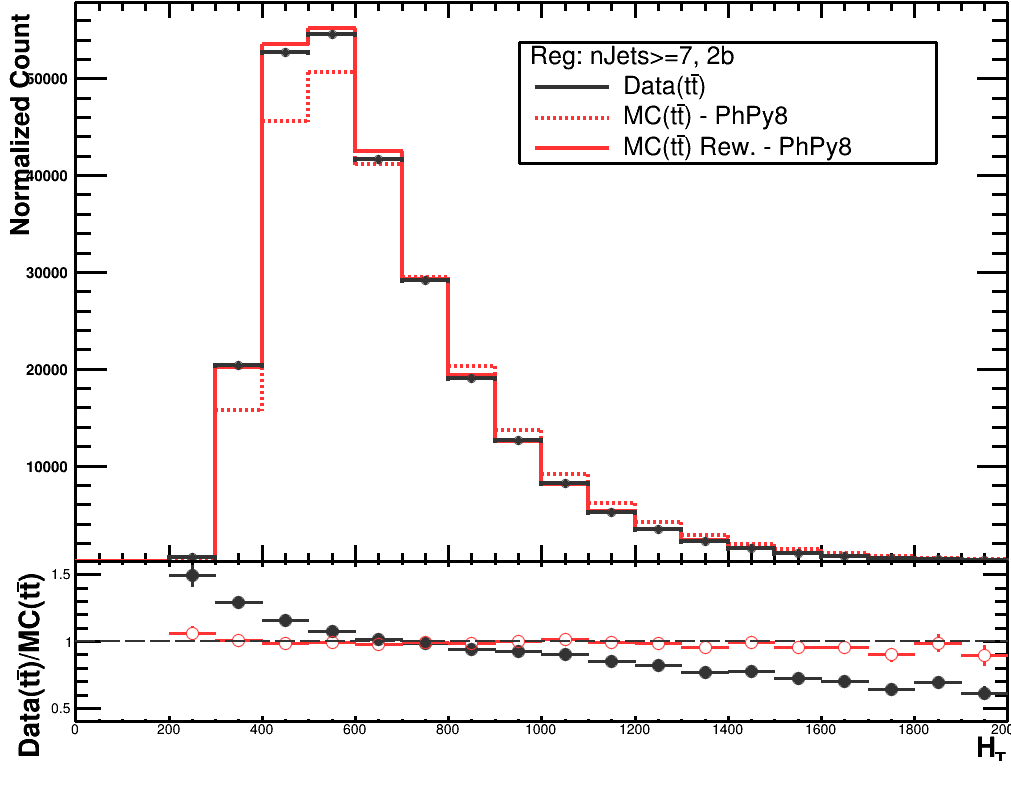
\includegraphics[width=0.48\textwidth]{plots/bkg_modelling/cor_1l_nom.png}
        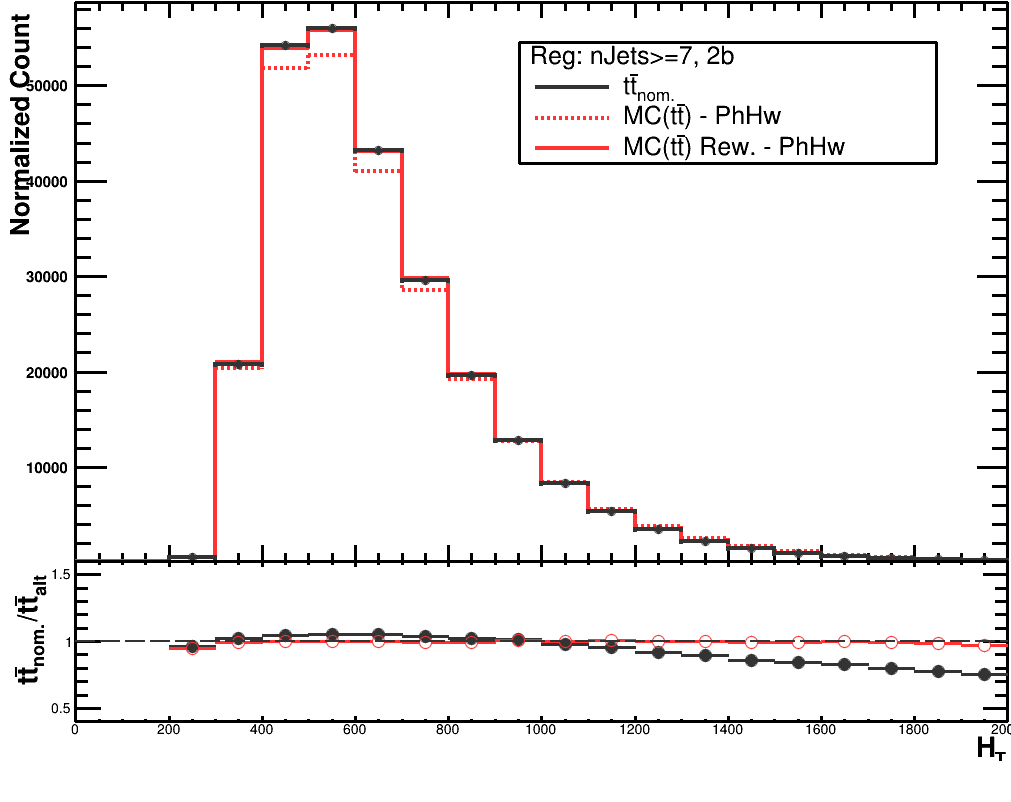
\includegraphics[width=0.48\textwidth]{plots/bkg_modelling/cor_1l_alt.png}
    \end{subfigure}
    \caption{The kinematic reweighting effect on $H_T$ distribution, and data/MC ratio for 1L \ttbar+jets nominal and one of the alternative samples. The black points in the ratio plot refer to data/MC ratio for the nominal MC samples with HF reweighting but without kinematic reweighting. The red points of the ratio plot refer to the data/MC ratio for the nominal MC samples after both HF and kinematic reweighting have been applied.}
    \label{fig::cor1l}
\end{figure}


\subsubsection{Uncertainty Propagation for NN Reweighting}
\label{sec:NN_reweighting:uncertainty}

Two additional uncertainties are considered to take into account the uncertainty on the data-driven
corrections. The reweighting factors on \ttbar + jets depend on the size of the non-\ttbar processes subtracted from data.
The cross section of the non-\ttbar processes is therefore varied by $\pm 50\%$ and alternative reweighting
factors are derived. The resulting difference in the final distribution is taken as a nuisance parameter in the
likelihood fit. The effect of this uncertainty ranges from 3\% to 4\%.

Understanding the influence of statistical uncertainty on background modeling aids in calibrating adjustments to the data within the fitted distributions.
Among the array of available methods in the literature, the Monte Carlo (MC) dropout method~\cite{gal2016dropout} was selected for its straightforward implementation and its flexibility in 
accommodating diverse neural network architectures. The dropout is originally a regularization method for neural networks where randomly selected neurons are ignored during training.
To apply this method following steps are considered,

\begin{itemize}
    \item {\bf Standard training:} Initialy a neural network is trained for reweighting factors without implementation of dropout layers.
    \item {\bf Dropout training:} A second training is considered with implementation of dropout layers into same architecture of standard training.
    \item {\bf Dropout evaluation:} The neural network from the dropout training is evaluated 1000 times by keep using dropout layers, so the random drops of neurons still remain, and results varied up in each iteration.
    \item {\bf Uncertainty propagation:} The standard deviation is calculated from the varied results of dropout evaluation. 
\end{itemize}


This method has been tested via toy and real data to understand better to effect of statistics on uncertainty.
For this example, we have created two different exponential distributions and matched them to each other through the neural network reweighting, and a fit function.
The uncertainty from the MC dropout method and the confidence interval at 68\% from the fit are compared in Figure~\ref{fig::unc_rew}, for poor and high statistics.
A similar test has been done on the training region by selecting different multiplicity of number of jets to observe how statistical fluctuation is effecting on this method in Figure~\ref{fig::unc_rew_real}

\begin{figure}[!htb]
    \centering
      (a)
      \begin{subfigure}[t]{\textwidth}
          \centering
          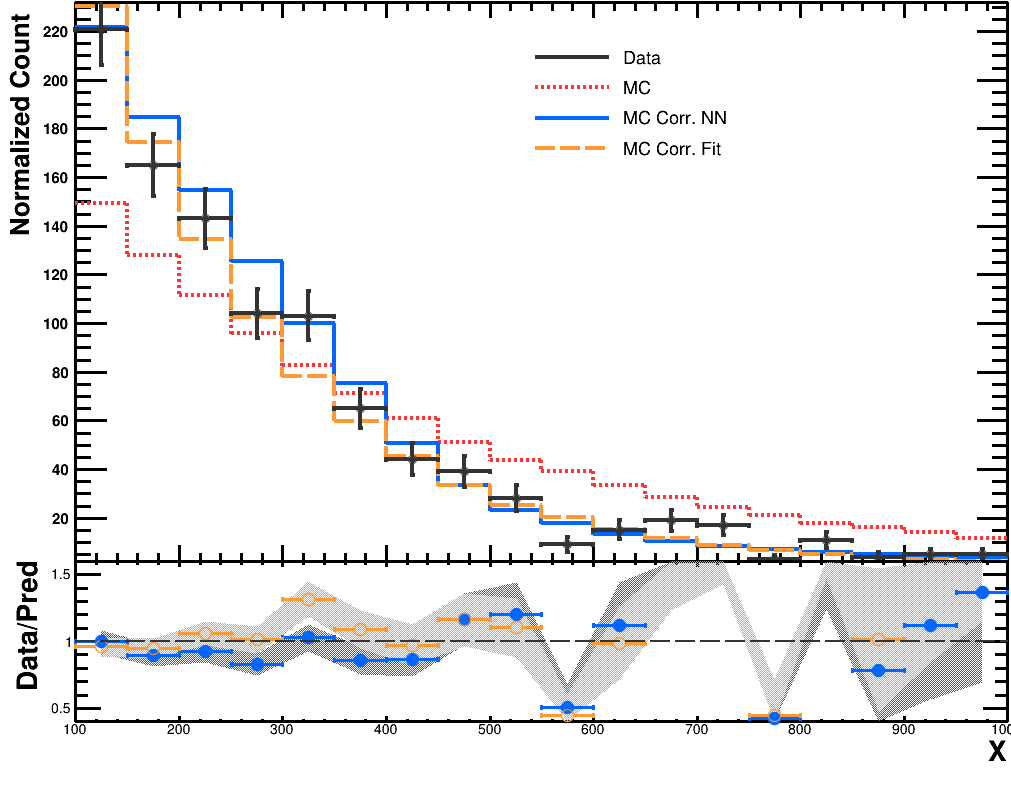
\includegraphics[width=0.48\textwidth]{plots/bkg_modelling/toy_poor.png}
          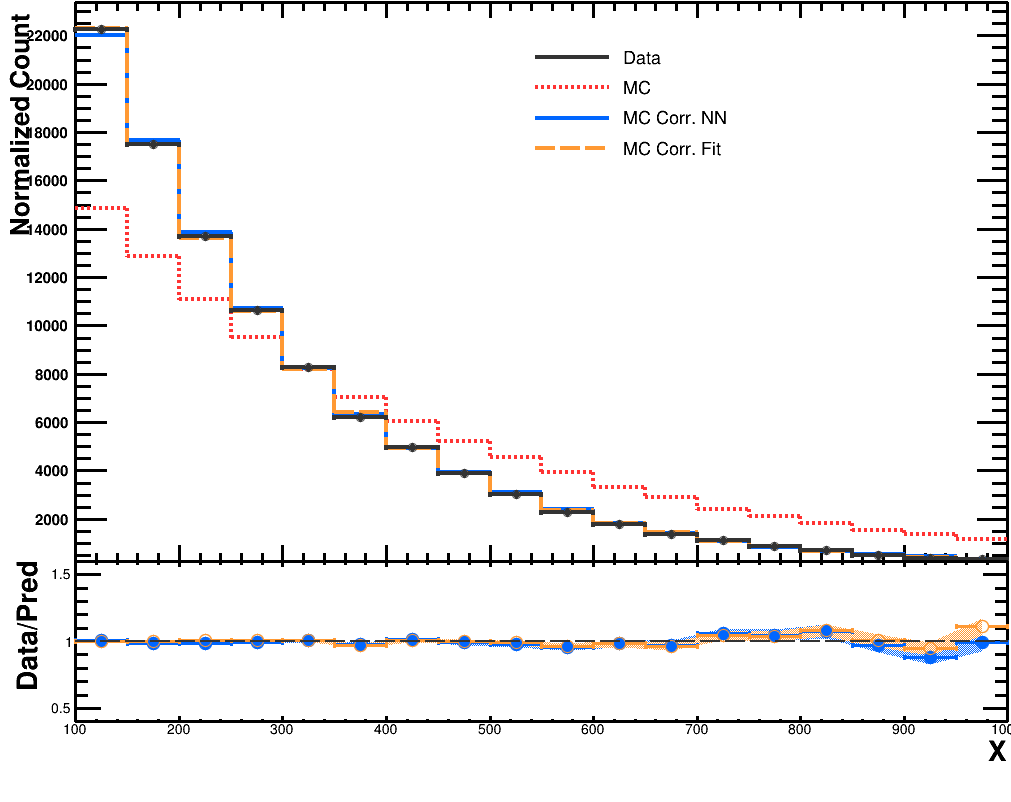
\includegraphics[width=0.48\textwidth]{plots/bkg_modelling/toy.png}
      \end{subfigure}
      (b)
      \begin{subfigure}[t]{\textwidth}
        \centering
        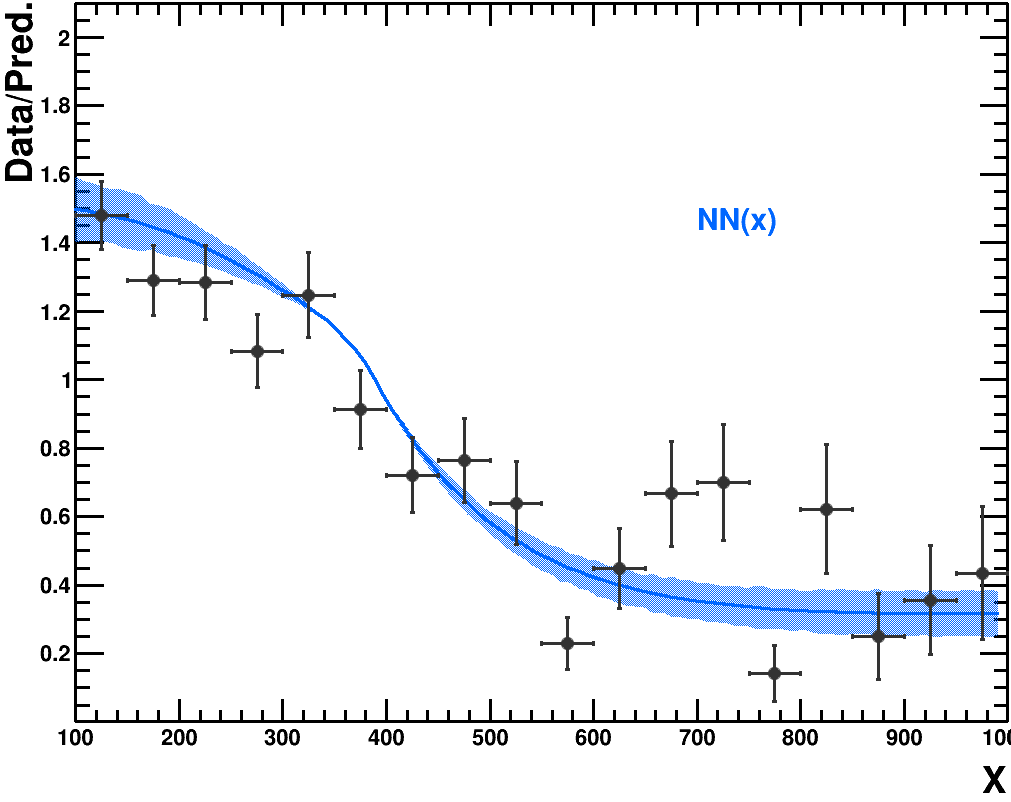
\includegraphics[width=0.48\textwidth]{plots/bkg_modelling/toy_nn_poor.png}
        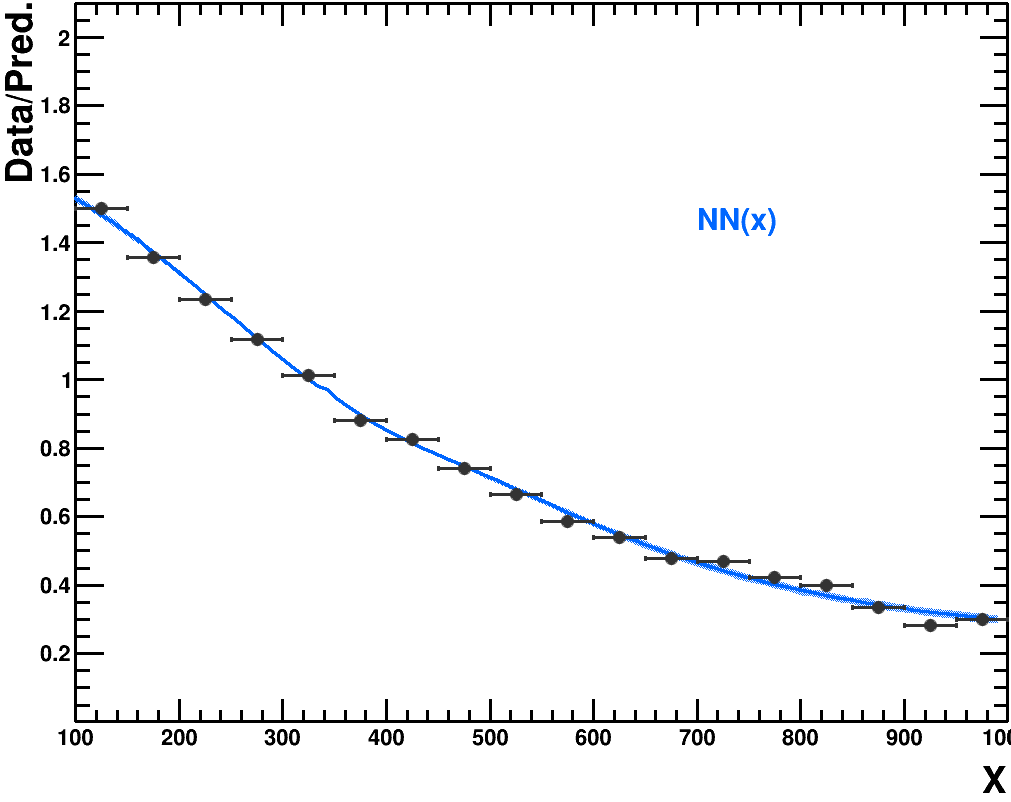
\includegraphics[width=0.48\textwidth]{plots/bkg_modelling/toy_nn.png}
      \end{subfigure}
      (c)
      \begin{subfigure}[t]{\textwidth}
        \centering
        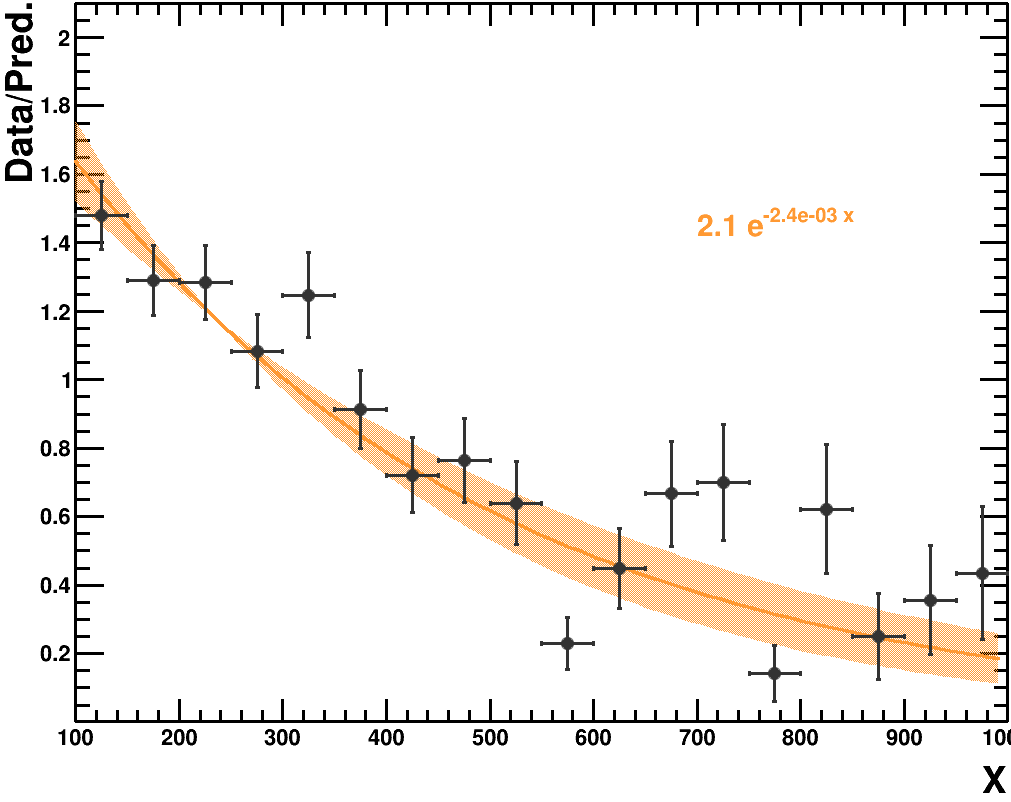
\includegraphics[width=0.48\textwidth]{plots/bkg_modelling/toy_fit_poor.png}
        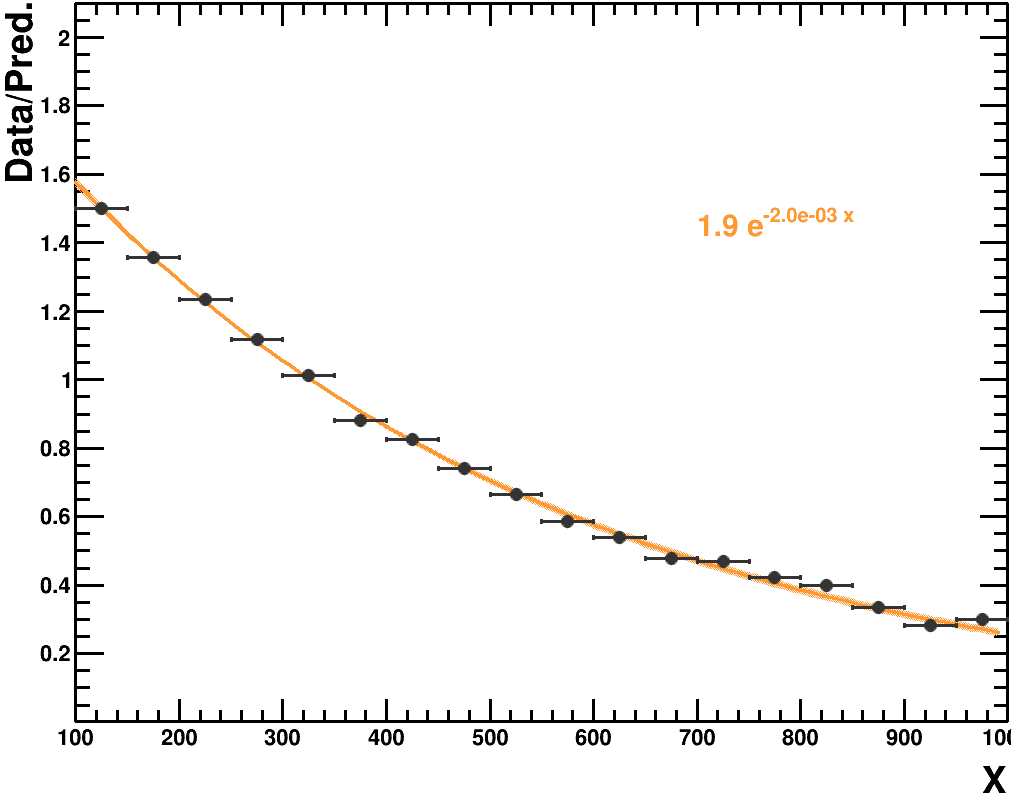
\includegraphics[width=0.48\textwidth]{plots/bkg_modelling/toy_fit.png}
      \end{subfigure}
     \caption{A toy example, generated randomly with two different coefficients of exponential function labeled as data and MC for 1000 (left), and 100000 (right) events.
     (a) Showing correction from NN reweighting and fit function with their uncertainty, (b) reweighting function from NN training and derived uncertainty,
     (c) fit function and the confidence interval at 68\%}
      \label{fig::unc_rew}
  \end{figure}

The given example in Figure~\ref{fig::unc_rew} shows a comparable effect of statistical error on the both NN, and fit modeling for background estimation. Therefore, the statistical errors on the derived reweighting factors are propagated through the MC dropout method, to the \ttbar +jets prediction and their impact are considered as nuisance parameters in the likelihood fit.

\begin{figure}[!htb]
    \centering
      (a)
      \begin{subfigure}[t]{\textwidth}
          \centering
          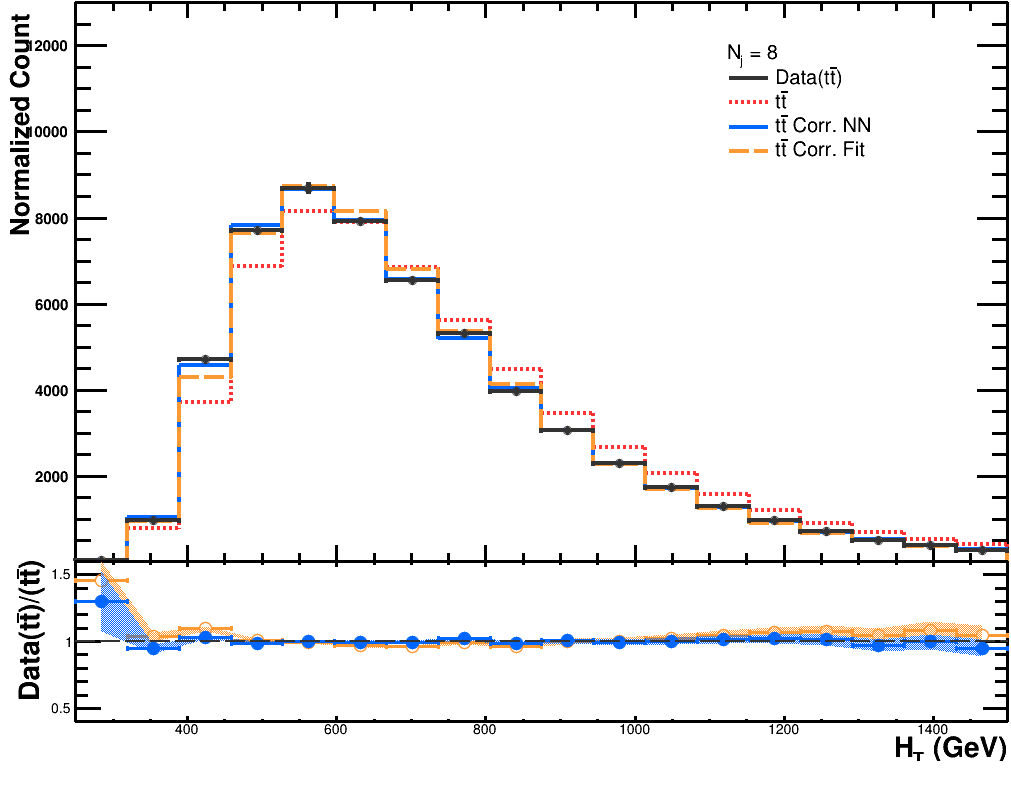
\includegraphics[width=0.48\textwidth]{plots/bkg_modelling/nn_rew_unc_real/val_8.png}
          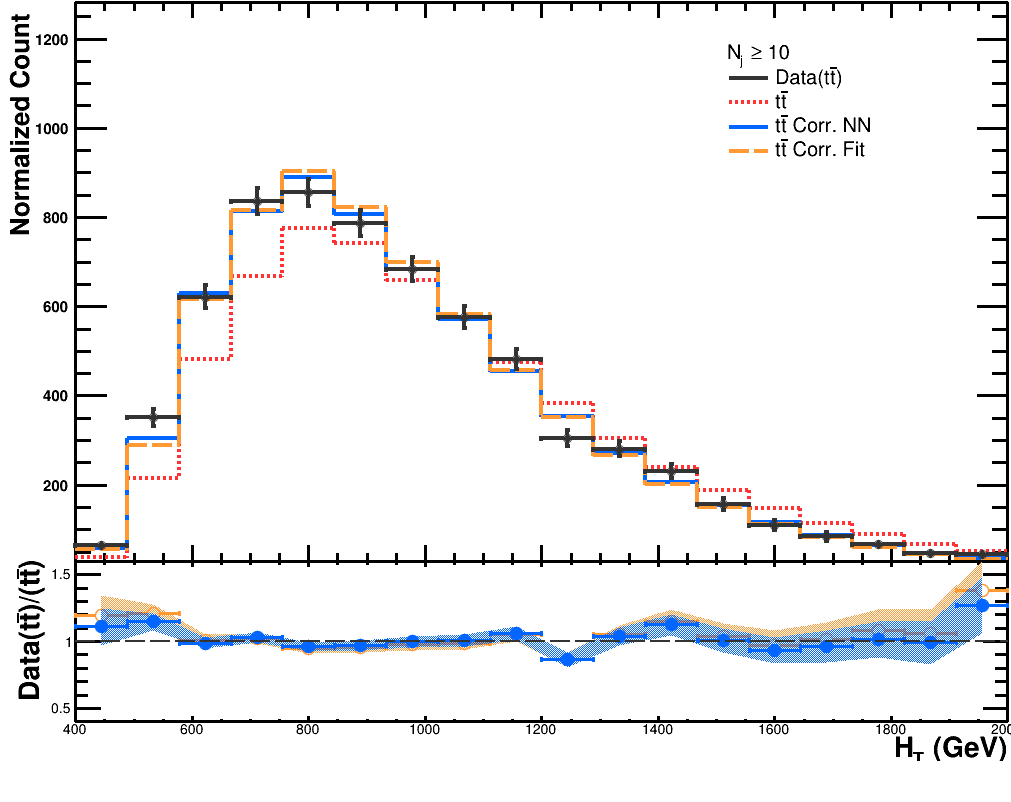
\includegraphics[width=0.48\textwidth]{plots/bkg_modelling/nn_rew_unc_real/val_geq10.png}
      \end{subfigure}
      (b)
      \begin{subfigure}[t]{\textwidth}
        \centering
        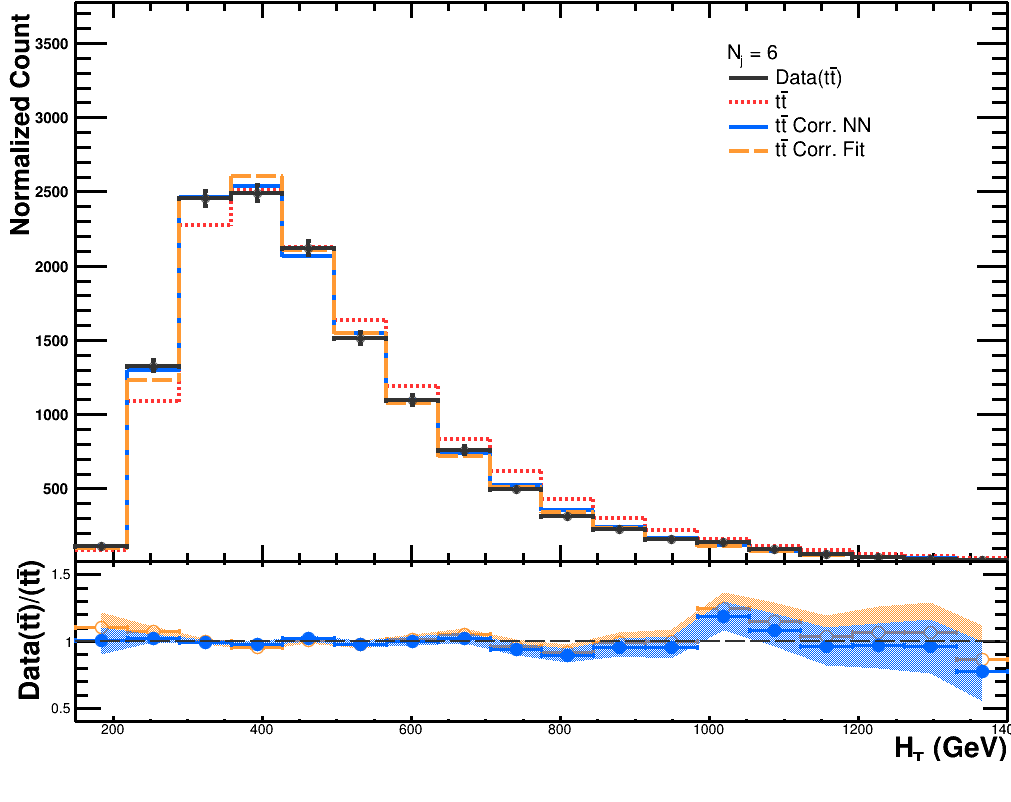
\includegraphics[width=0.48\textwidth]{plots/bkg_modelling/nn_rew_unc_real/val_2los_6.png}
        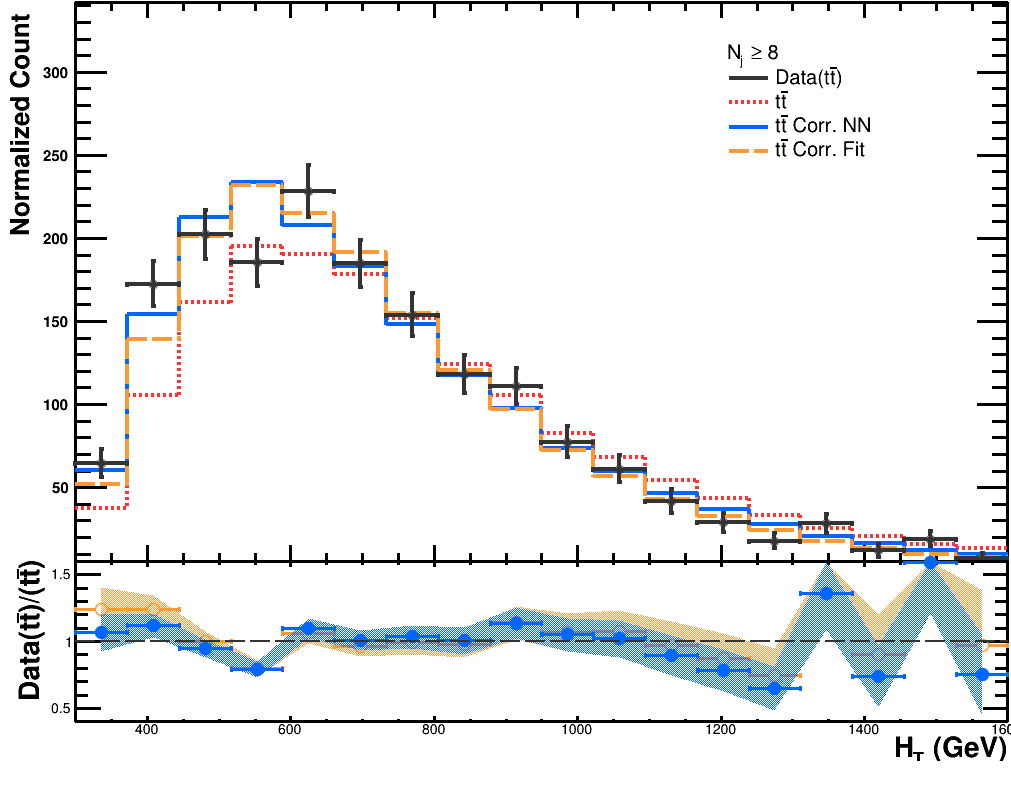
\includegraphics[width=0.48\textwidth]{plots/bkg_modelling/nn_rew_unc_real/val_2los_geq8.png}
      \end{subfigure}
     \caption{$H_{T}$ distributions with data/MC ratio for before and after correction from NN reweighting and MC dropout method, and fit modeling from two different coefficients of exponential function, and its confidence interval at 68\% (a) 1L, (b) (2LOS) channel, and left exclusive 8j(6j), right at least 10j(8j) jets multiplicities selections.}
      \label{fig::unc_rew_real}
  \end{figure}


%-------------------------------------------------------------------------------     


%-------------------------------------------------------------------------------                                                                                                
\FloatBarrier
\section{MVA strategy: signal extraction}
\label{sec:mva}
\subsection{Introduction}% Daniela, Nicola
\label{sec:mva_intro}
%
This search uses two discriminants to identify a possible signal over the large expected background rate from SM processes. 

A first discriminant based on Boosted Decision Trees (BDT)~\ref{sec:mva_bdt} is defined following similar studies performed in the context of the ATLAS measurement of SM production of four-top-quarks~\cite{ATLAS-CONF-2021-013}. The BDT is further optimised for this search as described in the following. A second dedicated discriminant is defined based on a Graph Neural Network~\ref{sec:mva_gnn}. 

The use of the BDT and GNN is combined with a novel structure which incorporates physics parameters of interest, in our case represented by the mass of the heavy Higgs boson \mH, as features for the training~\cite{Baldi_2016}, leading to a so-called parametrised classifier.
Parametrised classifiers provide smooth interpolation across physics parameters and improve the performance of isolated classifiers.
It is trained with signal samples at all mass benchmarks together against \ttbar background.
The training regions are chosen to be $\geq9j\geq3b$ for 1L and $\geq7j\geq3b$ for 2LOS channel.
The yields of signal samples and \ttbar background to train the BDT and GNN are shown in table~\ref{tab:MVAYields}.
The technical implementation is based on introducing a pseudo-mass feature in the background sample used for the training; this is a discrete variable assuming values between 400 to 1000~\gev\ in step of 100~\gev\ as available for the \ttH\ signal benchmarks. 
This pseudo-mass feature is also introduced for signal events as their truth \mH value. The pseudo-mass is treated as an additional input variable in the training. 

Over-training may occur when the performance of both BDT and GNN in the particular set of training samples is deviated from the performance in another set of samples.
It is checked by 2-fold cross-training in this analysis.
The samples are splitted into even and odd, based on the event index.
The output score of the model is evaluated by using the model trained on even events to evaluate odd events and vice-versa.
The area under ROC curve (AUC) is used as a performance metric and the difference between training and testing AUC is used as a metric of overtraining. 

Detailed comparative studies of the two discriminants were performed. The GNN and BDT discriminant modelling in signal depleted phase-spaces (see Sec.~\ref{sec:blinding}) was found to be satisfactory in both cases. The expected analysis sensitivity was observed to be significantly better with the GNN discriminant, leading to 20\%-10\% improvements in the expected exclusion limits depending on the assumed Higgs boson mass and lepton channel in consideration.  

The BDT and GNN discriminants are used both to perform a full analysis. The results for the GNN discriminant are taken as nominal, the results of the BDT analysis are used as cross check.

%%%Table: Yields of Signal and background of MVA Training%%% 
\begin{table}[h!]
\centering
\begin{tabular}{c|c|c|c|c|c|c|c|c}
\hline \hline
\multicolumn{9}{c}{1L Channel} \\
\hline
& $t\bar{t}+$ jets & M400 & M500 & M600 & M700 & M800 & M900 & M1000 \\
Unweighted Yields & 622925 & 26645 & 32370 & 36776 & 40119 & 42436 & 44555 & 46029 \\
Weighted Yields & 4760.97 & 59.90 & 72.34 & 81.59 & 88.60 & 93.29 & 97.8176 & 100.55 \\
\hline
\multicolumn{9}{c}{2LOS Channel} \\
\hline
& $t\bar{t}+$ jets & M400 & M500 & M600 & M700 & M800 & M900 & M1000 \\
Unweighted Yields & 135055 & 8999 & 10561 & 11807 & 12507 & 13225 & 13702 & 14238 \\
Weighted Yields & 1033.87 & 21.09 & 24.58 & 27.18 & 28.78 & 30.17 & 31.12 & 32.27 \\
\hline \hline
\end{tabular}
\caption{\label{tab:MVAYields}The unweighted and weighted yields of signal and \ttbar background used to train BDT and MVA.}
\end{table}


\subsection{Boosted Decision Trees}% Terry
\label{sec:mva_bdt}
%
\graphicspath{{figures/mva_bdt/}}
\subsubsection{Input variables}
\label{sec:BDT-input-variables}

BDT is trained for each mass point of Higgs boson $t\bar{t}H(\rightarrow t\bar{t})$ as signal and $t\bar{t}+$jets as background. 
All BDTs are using the same set of input variables, which are the variables retrieved from the SM$t\bar{t}t\bar{t}$ analysis plus some new variables that can improve the AUC performance. 
This section shows the 18 input variables used in the BDT for both 1L and OS channels.
The selected variables are divided into five groups based on different physics characteristics.

\begin{itemize}
\item \textbf{Global event activity in the transverse plan:}

$t\bar{t}H(\rightarrow t\bar{t})$ leads to more energetic and central activities than $t\bar{t}+$jets, especially the high mass Higgs boson signal.
Therefore the signal generally gives a larger value for the following variables than the $t\bar{t}+$jets background.
The heavier of BSM Higgs boson, the higher separation between the signal and background.

\begin{itemize}
\item The transverse momentum sum of all the reconstructed jets and leptons in the events ($H_{T}$)
\item Centrality of all reconstructed jets and leptons ($\sum_{i} {p_{T}}_{i} / \sum_{i} E_{i}$)  
\end{itemize}
\item \textbf{Jet activity:}

$t\bar{t}H(\rightarrow t\bar{t})$ generates more hard jets than $t\bar{t}+$jets.
The following variables get a boosted value in $t\bar{t}H(\rightarrow t\bar{t})$.

\begin{itemize}
\item Jet multiplicity ($N_{jets}$)
\item Transverse momentum of leading jet (${p_{T}}_{0}$)
\end{itemize}

The extra jets from $t\bar{t}+$jets are mainly from the radiation while high jet multiplicity is mainly come from the prompt particles in $t\bar{t}H(\rightarrow t\bar{t})$
The radiation jets highly affected the separation between jets and the invariant mass of jets with angular threshold.
The following variables are used to compare the radiation structure between signal and background.

\begin{itemize}
\item Average angular separation across all pairs of jets ($\Delta R^{avg}_{jj}$)
\item Invariant mass of the triplet jets with minimum angular separation~\footnote{The angular separation of triplet of jets is defined as $\Delta R_{ijk}=\sqrt{\Delta R^{2}_{ij}+\Delta R^{2}_{ik}+\Delta R^{2}_{jk}}$, where $i$, $j$ and $k$ are the indices of the three jets} ($M^{min. \Delta R}_{jjj}$)
\item Average invariant mass of all the jets triplets with angular separation smaller than three ($M^{\Delta R<3}_{jjj}$)
\end{itemize}

In 1L-channel, it is expected that four hard jets are directly come from top-quarks in $t\bar{t}$+jets, while the remaining jets are generally the soft radiation.
In contrast, ten hard jets are expected come from top-quarks in $t\bar{t}H(\rightarrow t\bar{t})$. 
The following variable shows the properties between first few leading hard jets and the remaining soft jets among $t\bar{t}H(\rightarrow t\bar{t})$ and $t\bar{t}$+jets.

\begin{itemize}
\item The ratio of transverse momentum sum of the first four leading jets to the transverse momentum sum of the remaining jets ($\sum^{3}_{i=0}{p_{T}}_{i} / \sum_{i\geq 4} {p_{T}}_{i}$)
\end{itemize}

\item \textbf{b-tagging information}

$t\bar{t}H(\rightarrow t\bar{t})$ generates more energetic b-jets with respective to $t\bar{t}+$jets, where extra b-tagged jets are come from radiation.
The energy of b-jets is higher in $t\bar{t}H(\rightarrow t\bar{t})$ with heavier Higgs boson.
The b-tagging working point used for these variables is defined as DL1r 70\%.
The following variables related with b-tagged jets properties give a separation between signal and background.

\begin{itemize}
\item Minimum angular separation among all pairs of b-tagged jets and leptons ($\Delta R^{min}_{bl}$)
\item Minimum angular separation among all pairs of b-tagged jets ($\Delta R^{min}_{bb}$)
\item Average invariant mass of all the b-tagged jets triplets ($M^{avg}_{bbb}$)
\item Minimum invariant mass of all pairs of b-tagged jets ($M^{min}_{bb}$)
\item Sum of the pseudo continuous b-tagged score of the four leading jets ranked in DL1r score ($\sum^{i<4}_{i=0} {pcb}_{i}$)
\end{itemize}

\item \textbf{RC-jets information}

$t\bar{t}H(\rightarrow t\bar{t})$ gets more jets activities in the transverse plan and some of the produced top-quarks could be boosted, especially for the heavy Higgs boson signal.
This boosted structure can be re-clustered into large-R jets with sub-structure that are not favour in $t\bar{t}+$jets.

\begin{itemize}
\item Number of RC-jets with a mass higher than 100 GeV ($N_{RC100}$)
\item Sum of the first $k_{T}$ splitting scale $d_{12}$ of all RC-jets ($\sum d_{12}$)~\footnote{The $k_{T}$ splitting scale $d_{ij}$ is defined as the recombination distance between the jets constituent from a $k_{t}$ algorithm: $d_{ij}=min({p_{T}}_{i}^{2},{p_{T}}_{j}^{2})\times \Delta R^{2}_{ij}$.}
\item Sum of the second $k_{T}$ splitting scale $d_{23}$ of all RC-jets ($\sum d_{23}$)
\end{itemize}

\item \textbf{Leptons and neutrino activities:}
The leptons are expected from the W-boson which is decayed from top-quark.
$t\bar{t}H(\rightarrow t\bar{t})$ generally leads to more energetic leptons and neutrinos (which is described in miss transverse momentum MET) than $t\bar{t}$+jets, especially for the heavy Higgs boson.
The following variables describe the leptonic activities of the events.

\begin{itemize}
\item Missing transverse momentum ($E^{miss}_{T}$)
\item W reconstructed transverse mass ($m_{T}(\ell,E^{miss}_{T})$) for 1L and the invariant mass of two leptons ($m_{\ell \ell}$) in OS.
\end{itemize}

\end{itemize} 

Several input variables distributions, with separation power defined as
%%%%Equation: Variable Separation%%%%
\begin{equation}
\mathrm{Sep}=\frac{1}{2}\sum_{\mathrm{bins}} \frac{(s-b)^{2}}{s+b}~,
\label{eqn:varSeparation}
\end{equation}
%%%%%%%%%%%%%%%%%%%%%%%%%%%%%%%%%%%%%%%
where $s$ and $b$ are the signal and background ($t\bar{t}+\mathrm{jets}$) yields respectively of each bin, are shown in Figure~\ref{fig:1L_inputVarDistribution} and the correlation between them are shown in Figure~\ref{fig:1L_inputVarCorrelation}.

%%%%%%%%%%%%%%%%%%%%%%%%%%%%%%%%%%%%%%%
where $s$ and $b$ are the signal and background ($t\bar{t}+\mathrm{jets}$) yields respectively of each bin. 

%%%%Fig: Input Variables Plots%%%%
\begin{figure}[!htp]
    \centering
    \begin{subfigure}[t]{0.32\textwidth}
        \centering
        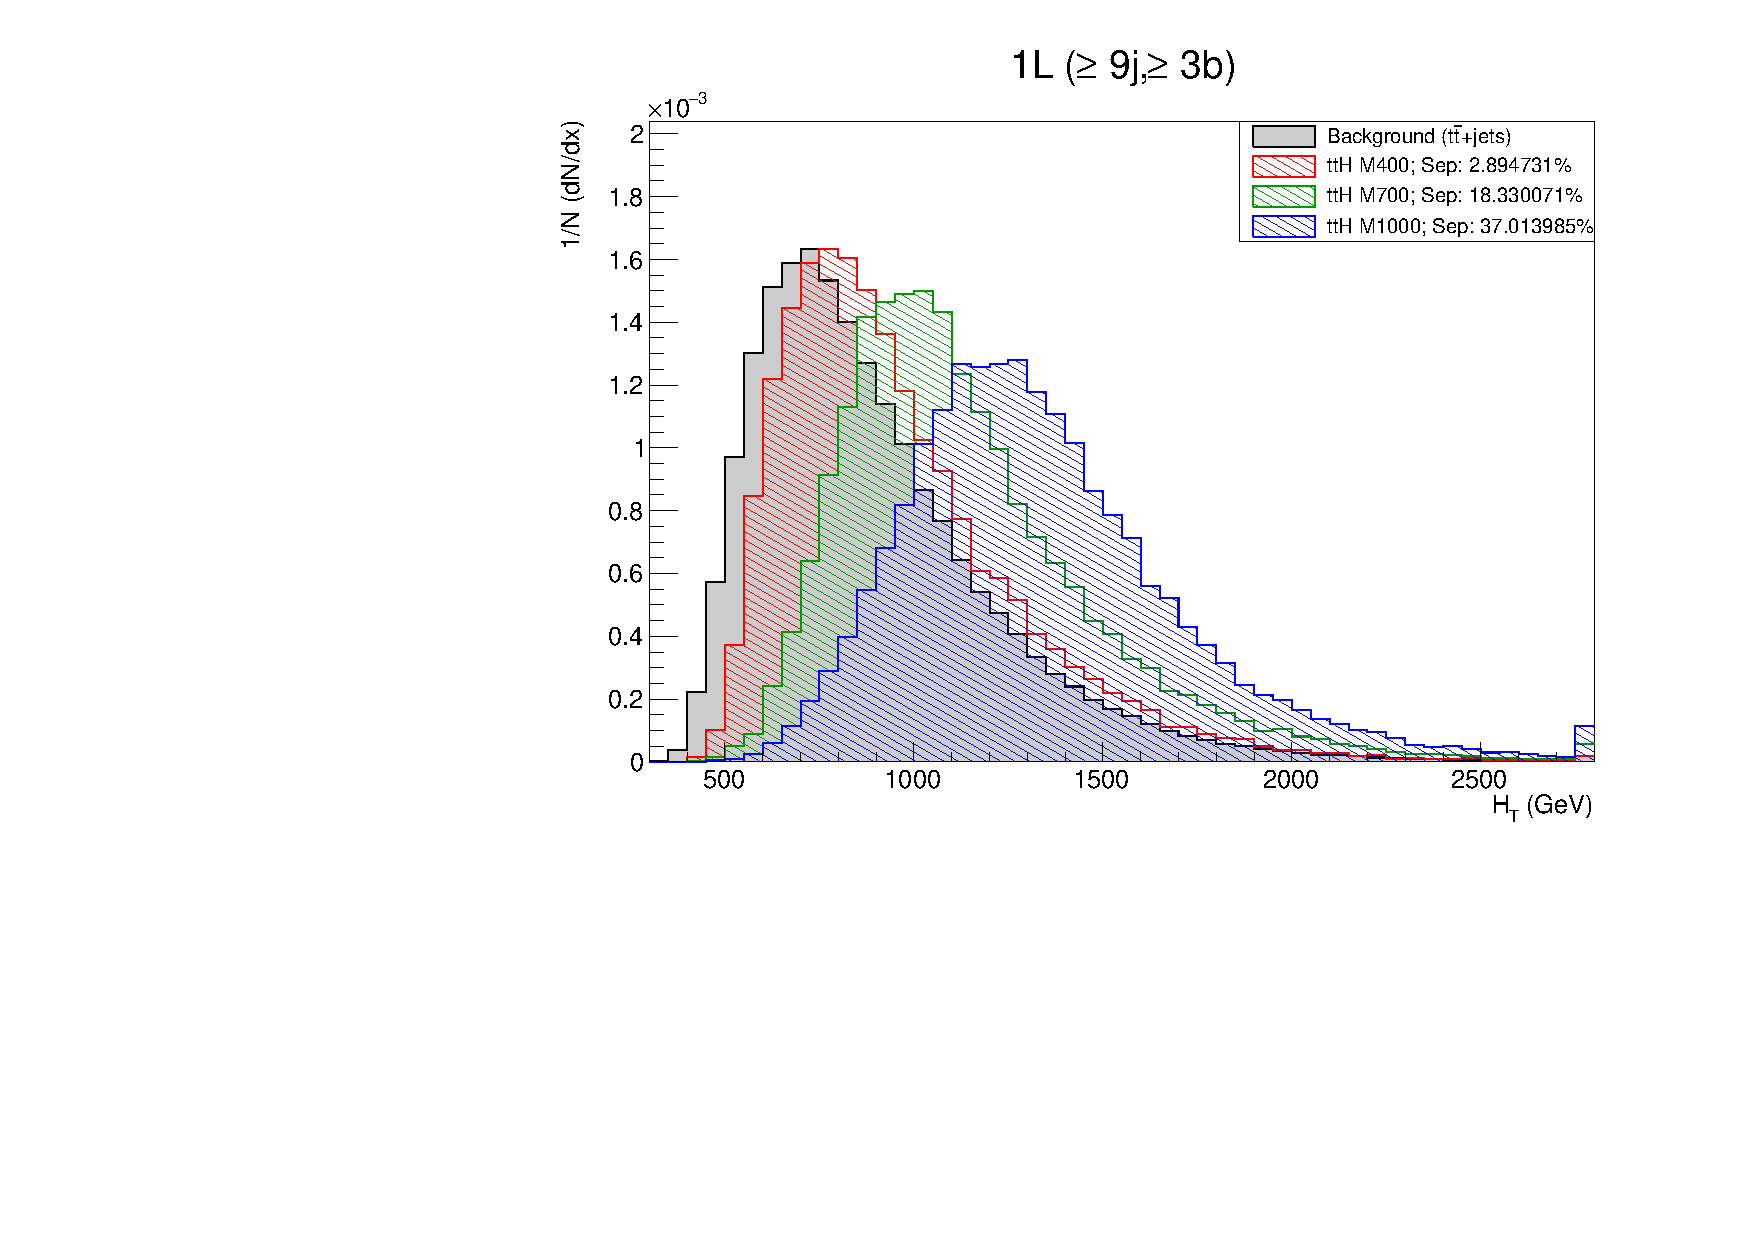
\includegraphics[width=\textwidth]{inputVar/1L/HT_all_ljets_ge9jge3b.pdf}
        \subcaption{$H_{T}$}
    \end{subfigure}
    \begin{subfigure}[t]{0.32\textwidth}
        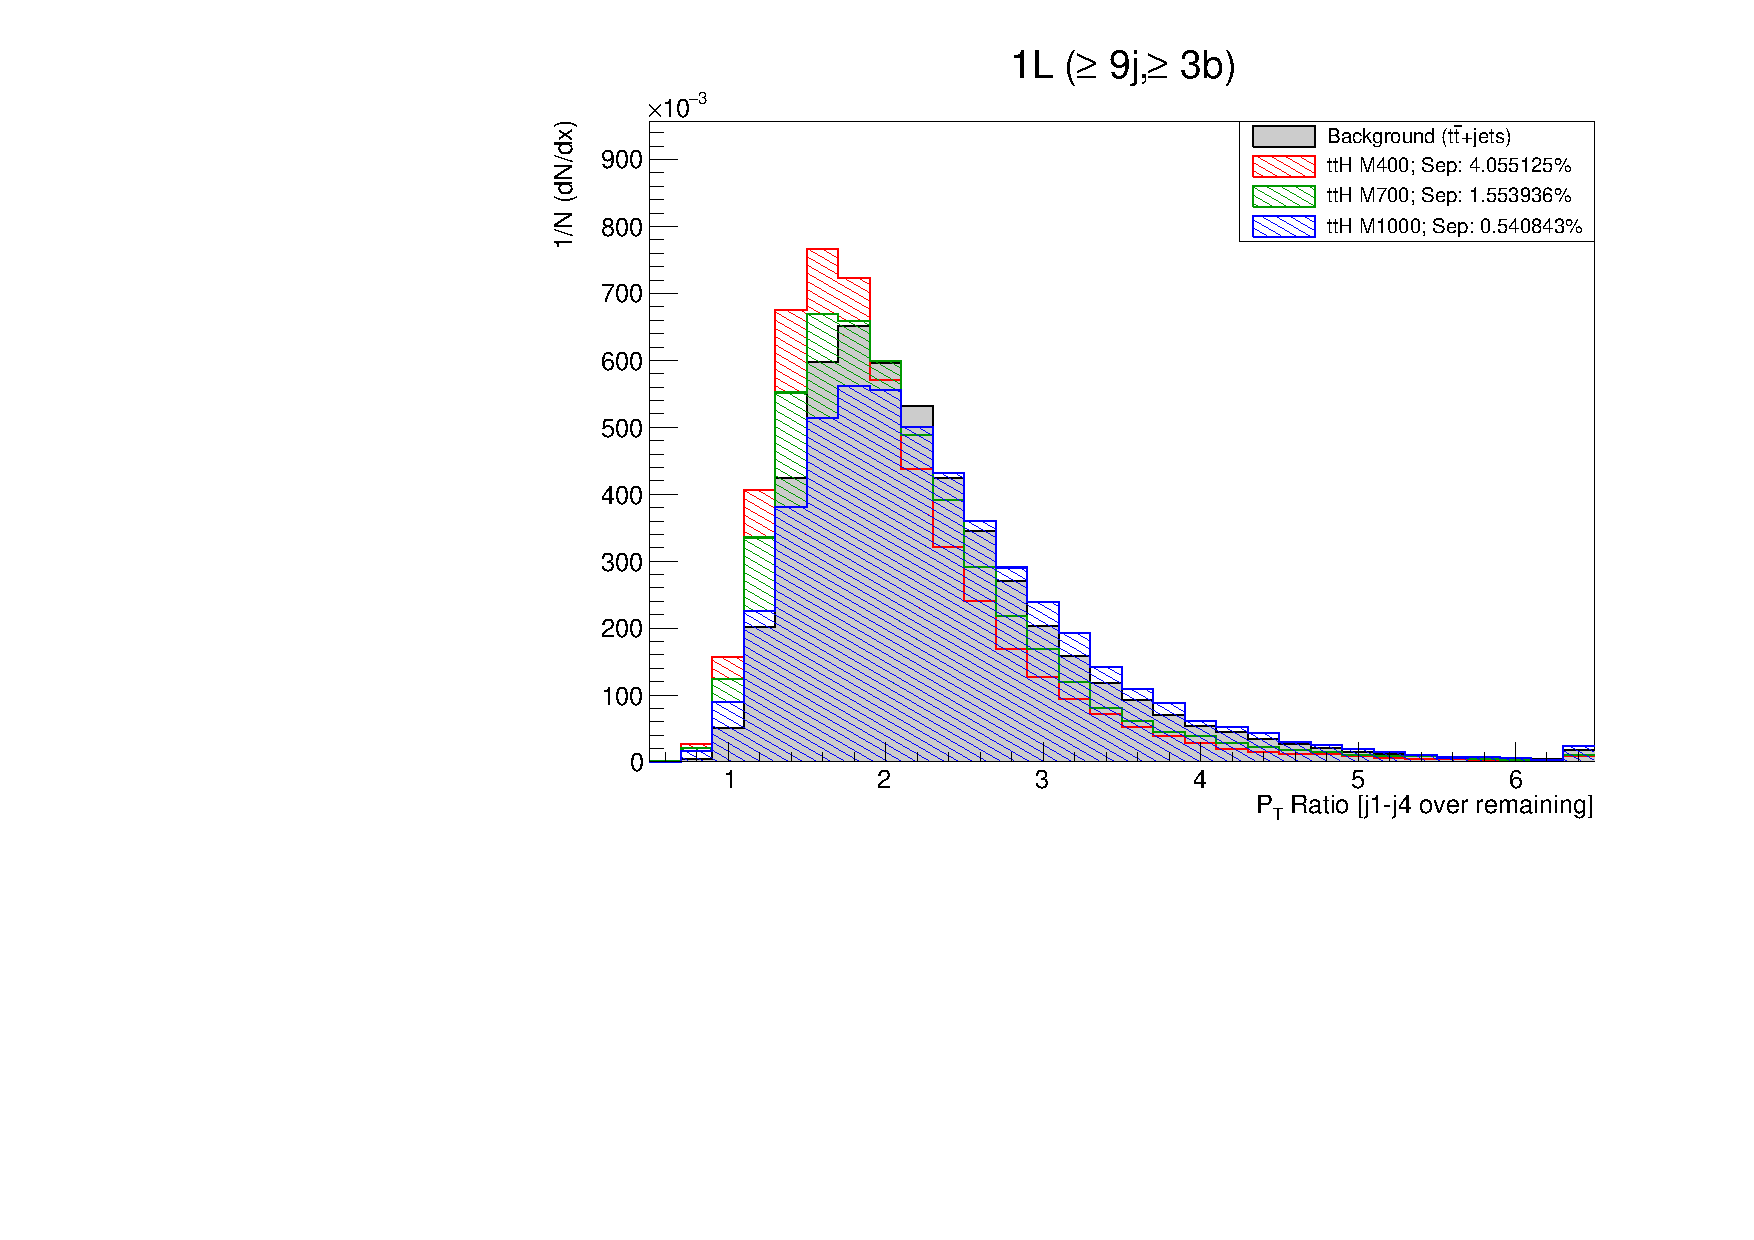
\includegraphics[width=\textwidth]{inputVar/1L/HT_rat_ljets_ge9jge3b.pdf}
        \subcaption{$\sum^{3}_{i=0}{p_{T}}_{i} / \sum_{i\geq 4} {p_{T}}_{i}$}
    \end{subfigure}
    \begin{subfigure}[t]{0.32\textwidth}
        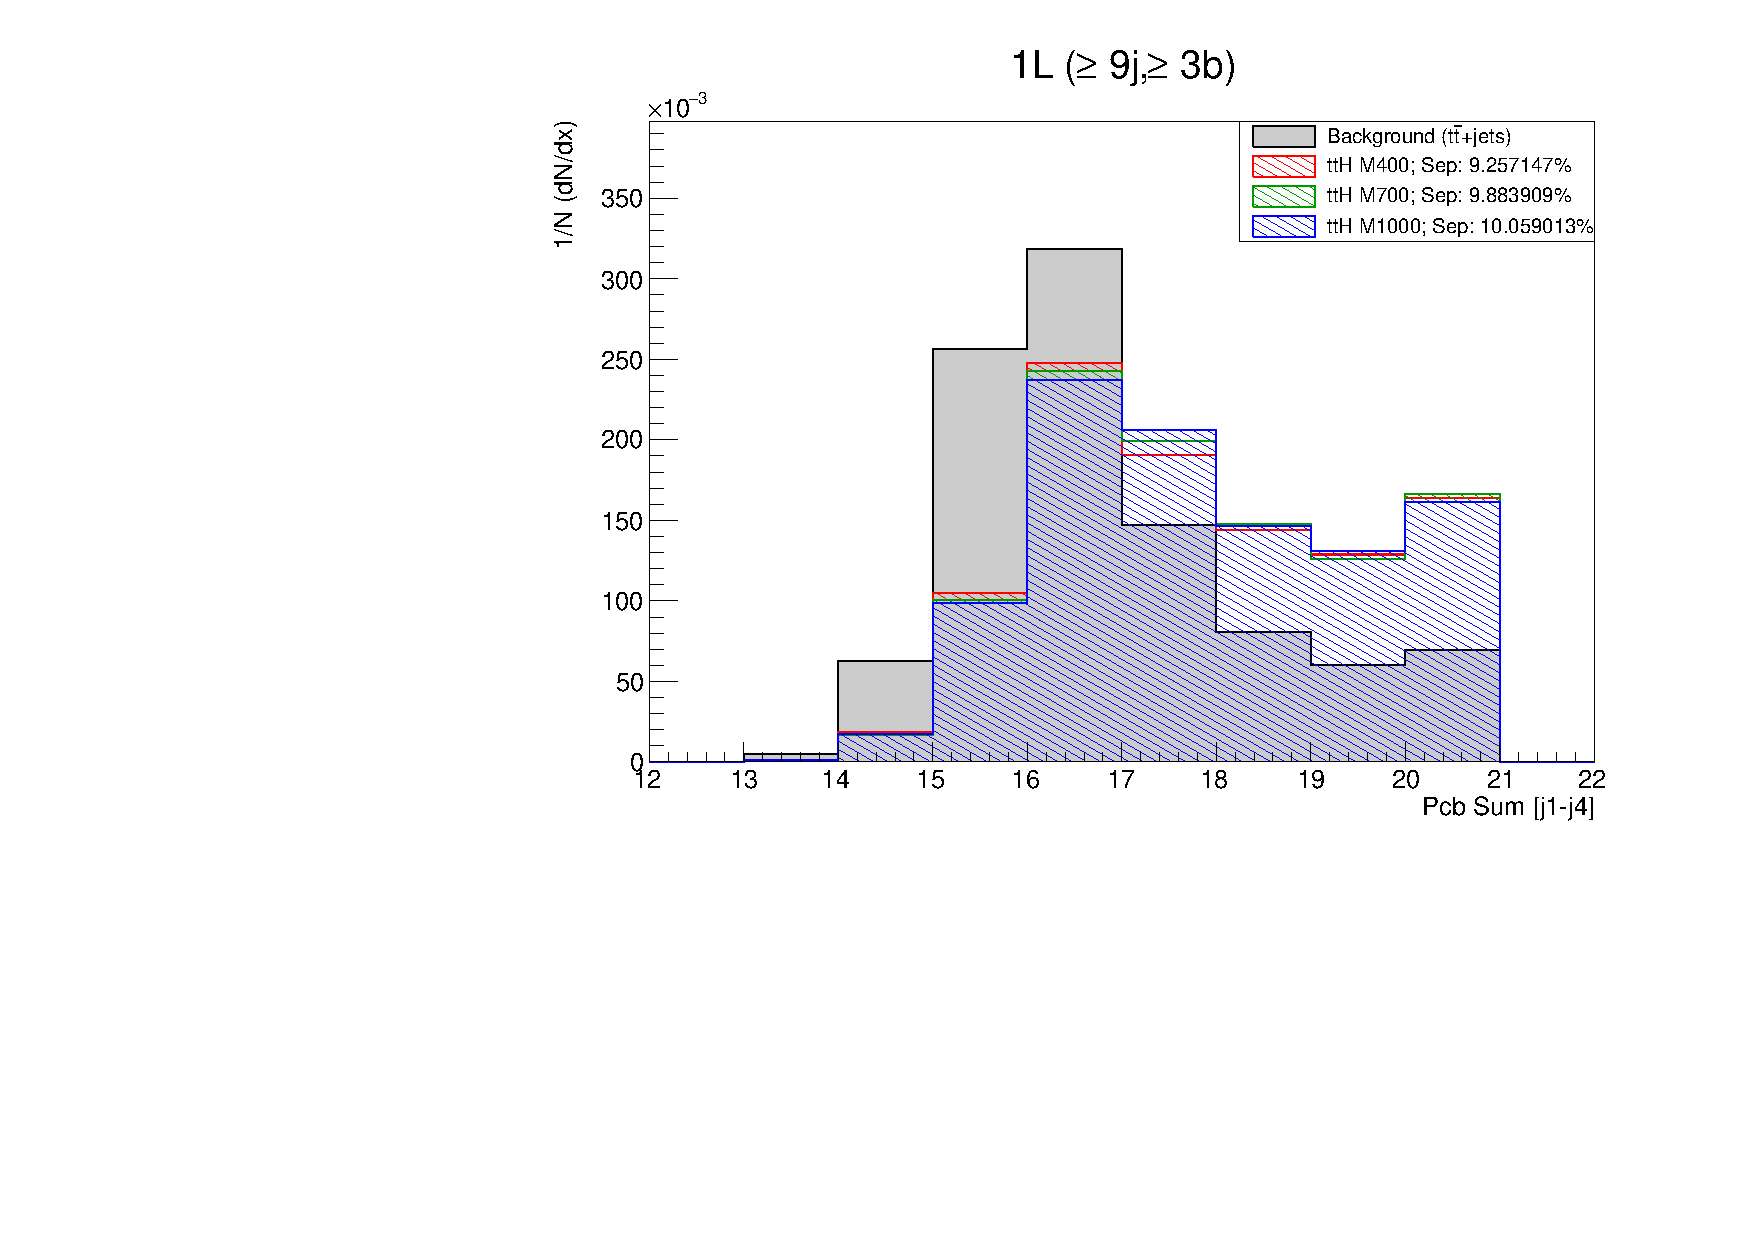
\includegraphics[width=\textwidth]{inputVar/1L/pcbSum_ljets_ge9jge3b.pdf}
        \subcaption{$\sum^{i<4}_{i=0} {pcb}_{i}$}
    \end{subfigure}
    \newline
    \begin{subfigure}[t]{0.49\textwidth}
        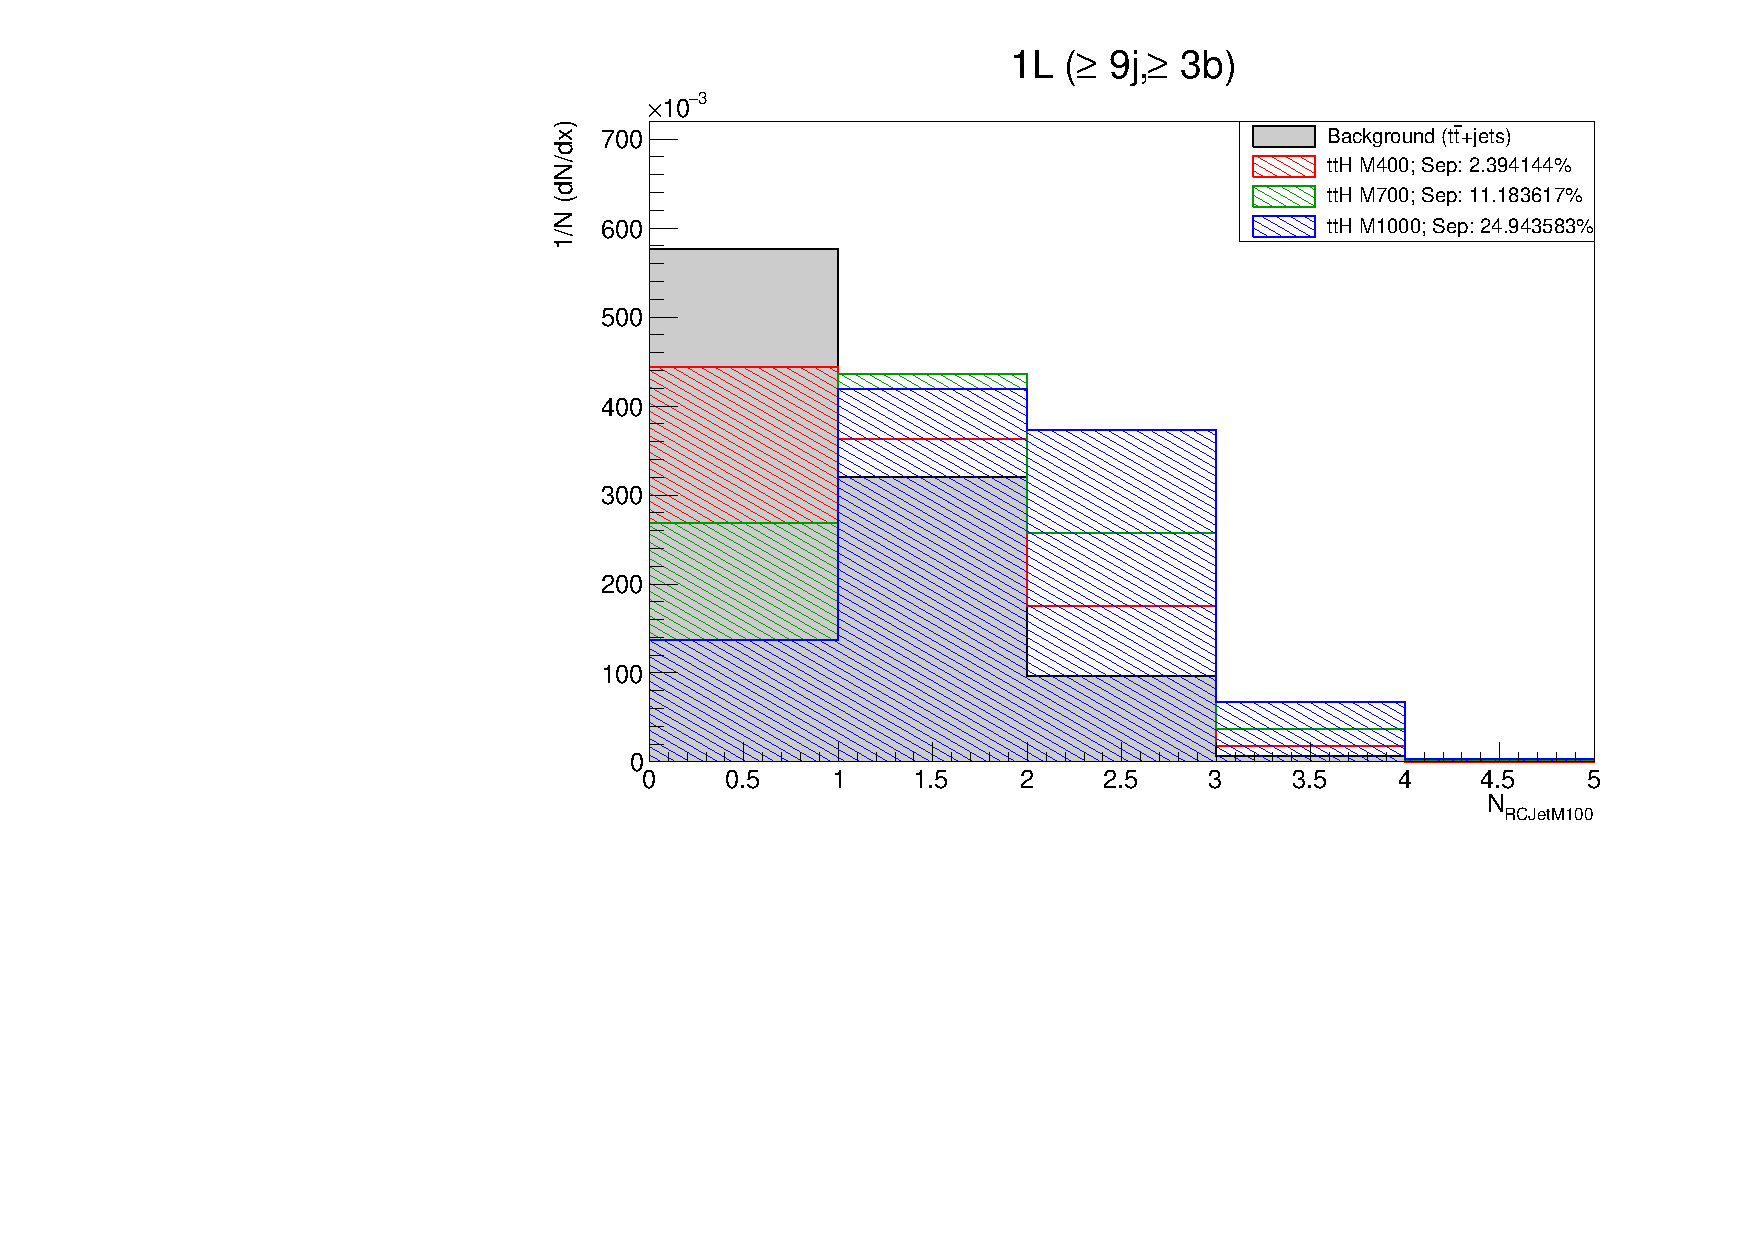
\includegraphics[width=\textwidth]{inputVar/1L/nRCJetsM100_ljets_ge9jge3b.pdf}
        \subcaption{$N_{RC100}$}
    \end{subfigure}
    \begin{subfigure}[t]{0.49\textwidth}
        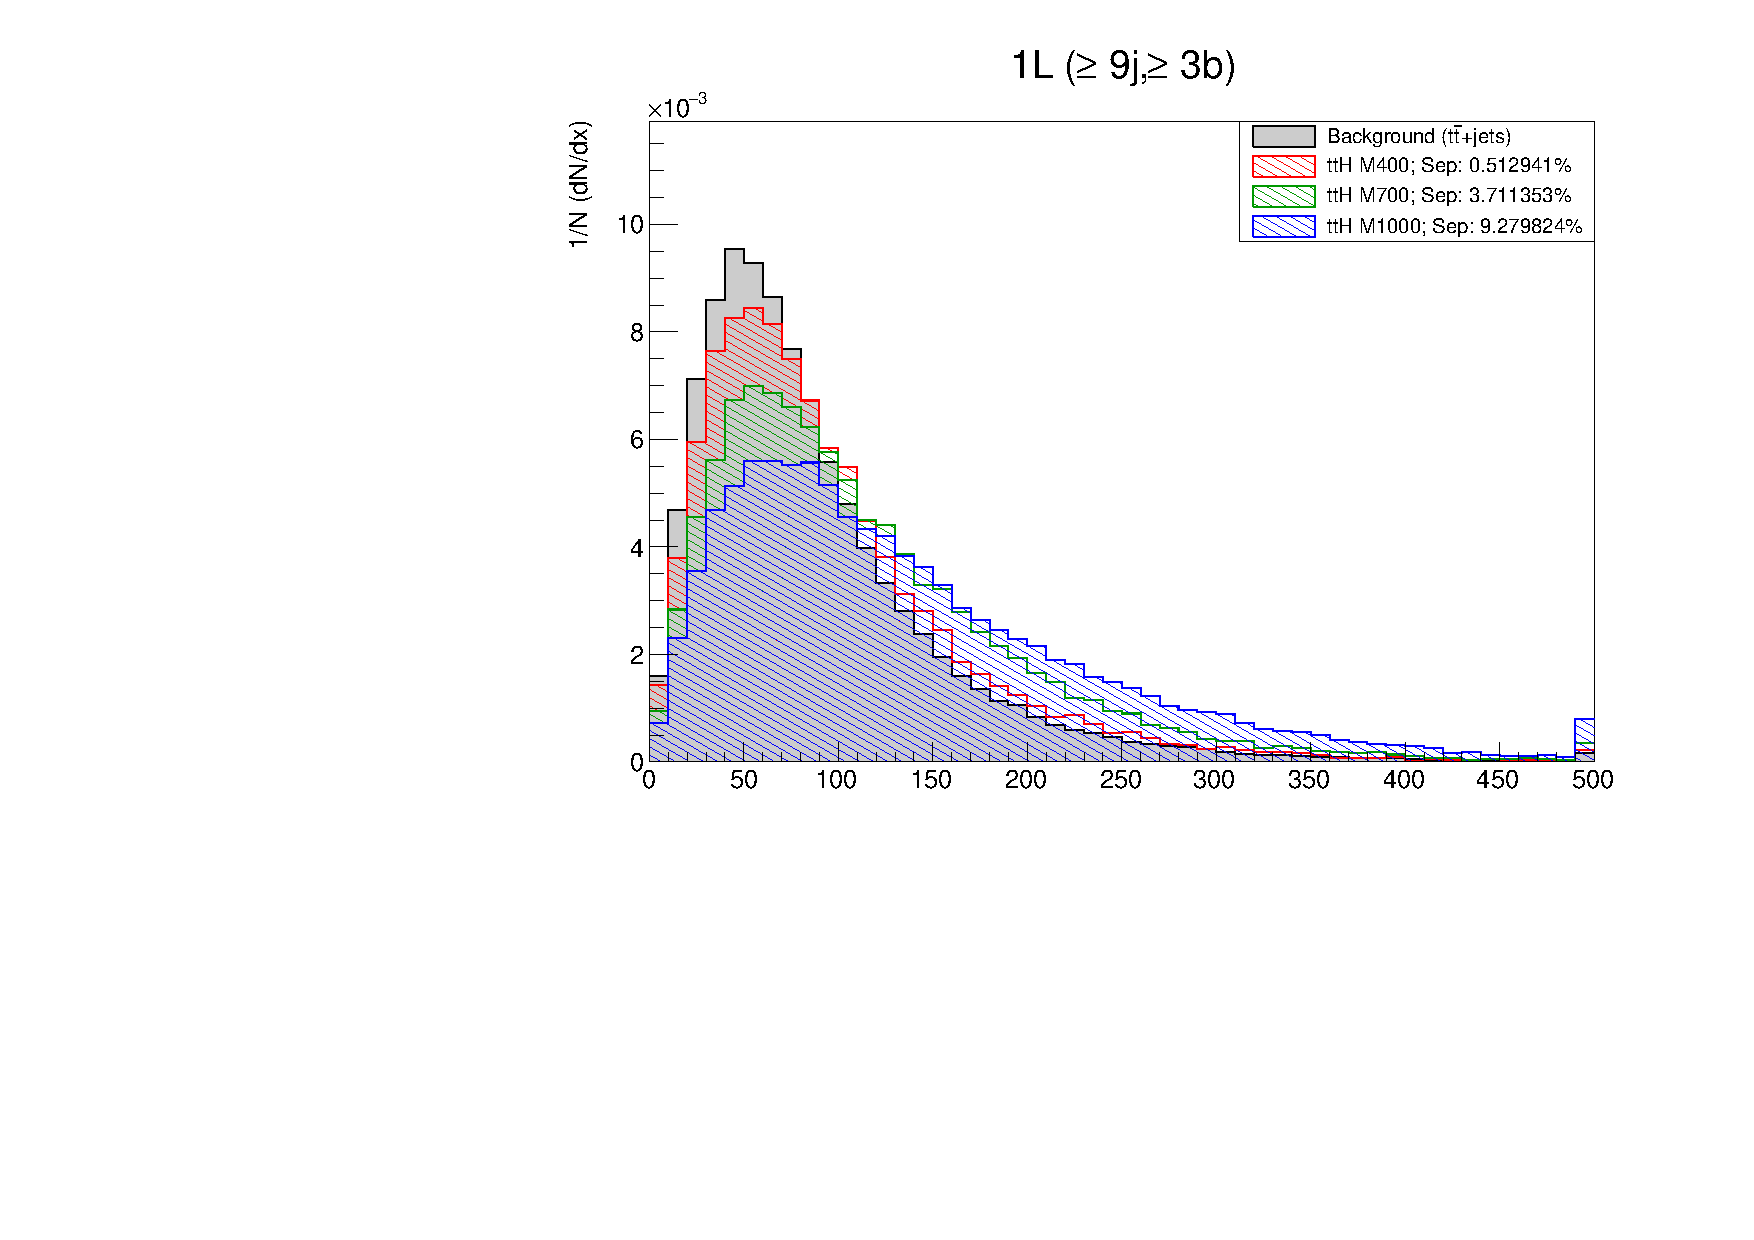
\includegraphics[width=\textwidth]{inputVar/1L/met_met_ljets_ge9jge3b.pdf}
        \subcaption{$E^{miss}_{T}$}
    \end{subfigure}
    \caption{\label{fig:1L_inputVarDistribution}Some input variables distribution of $t\bar{t}$+jets, and $t\bar{t}H(\rightarrow t\bar{t})$ with BSM Higgs boson mass of 400 GeV, 700 GeV and 1000 GeV in the region of $\geq9j \geq 3b$. The distributions are normalized to one.}
\end{figure}
%%%%%%%%

%%%% Fig: Input Variable Correlation %%%%
\begin{figure}[!htp]
    \centering
        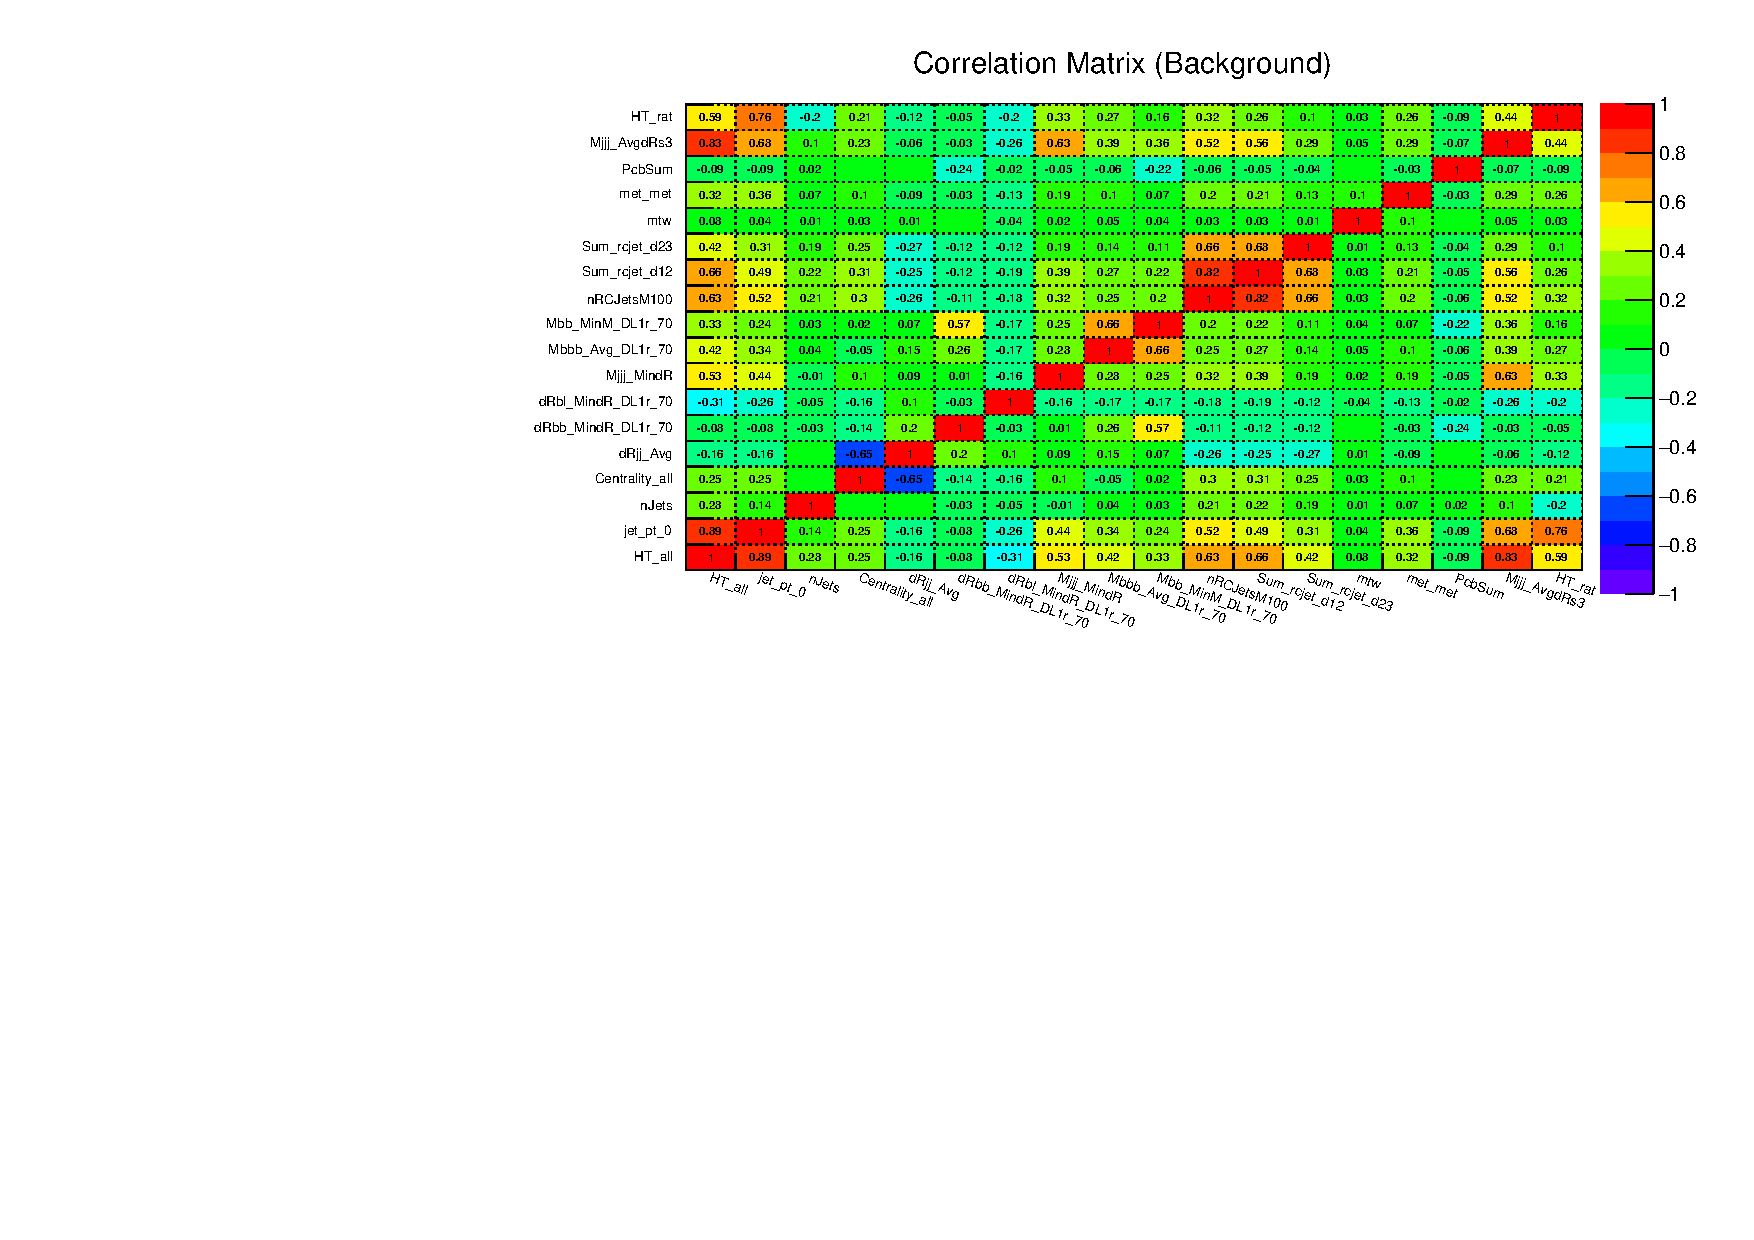
\includegraphics[width=0.55\textwidth]{inputVar_correlation/1L_correlation_ttbar.pdf}
    \newline
        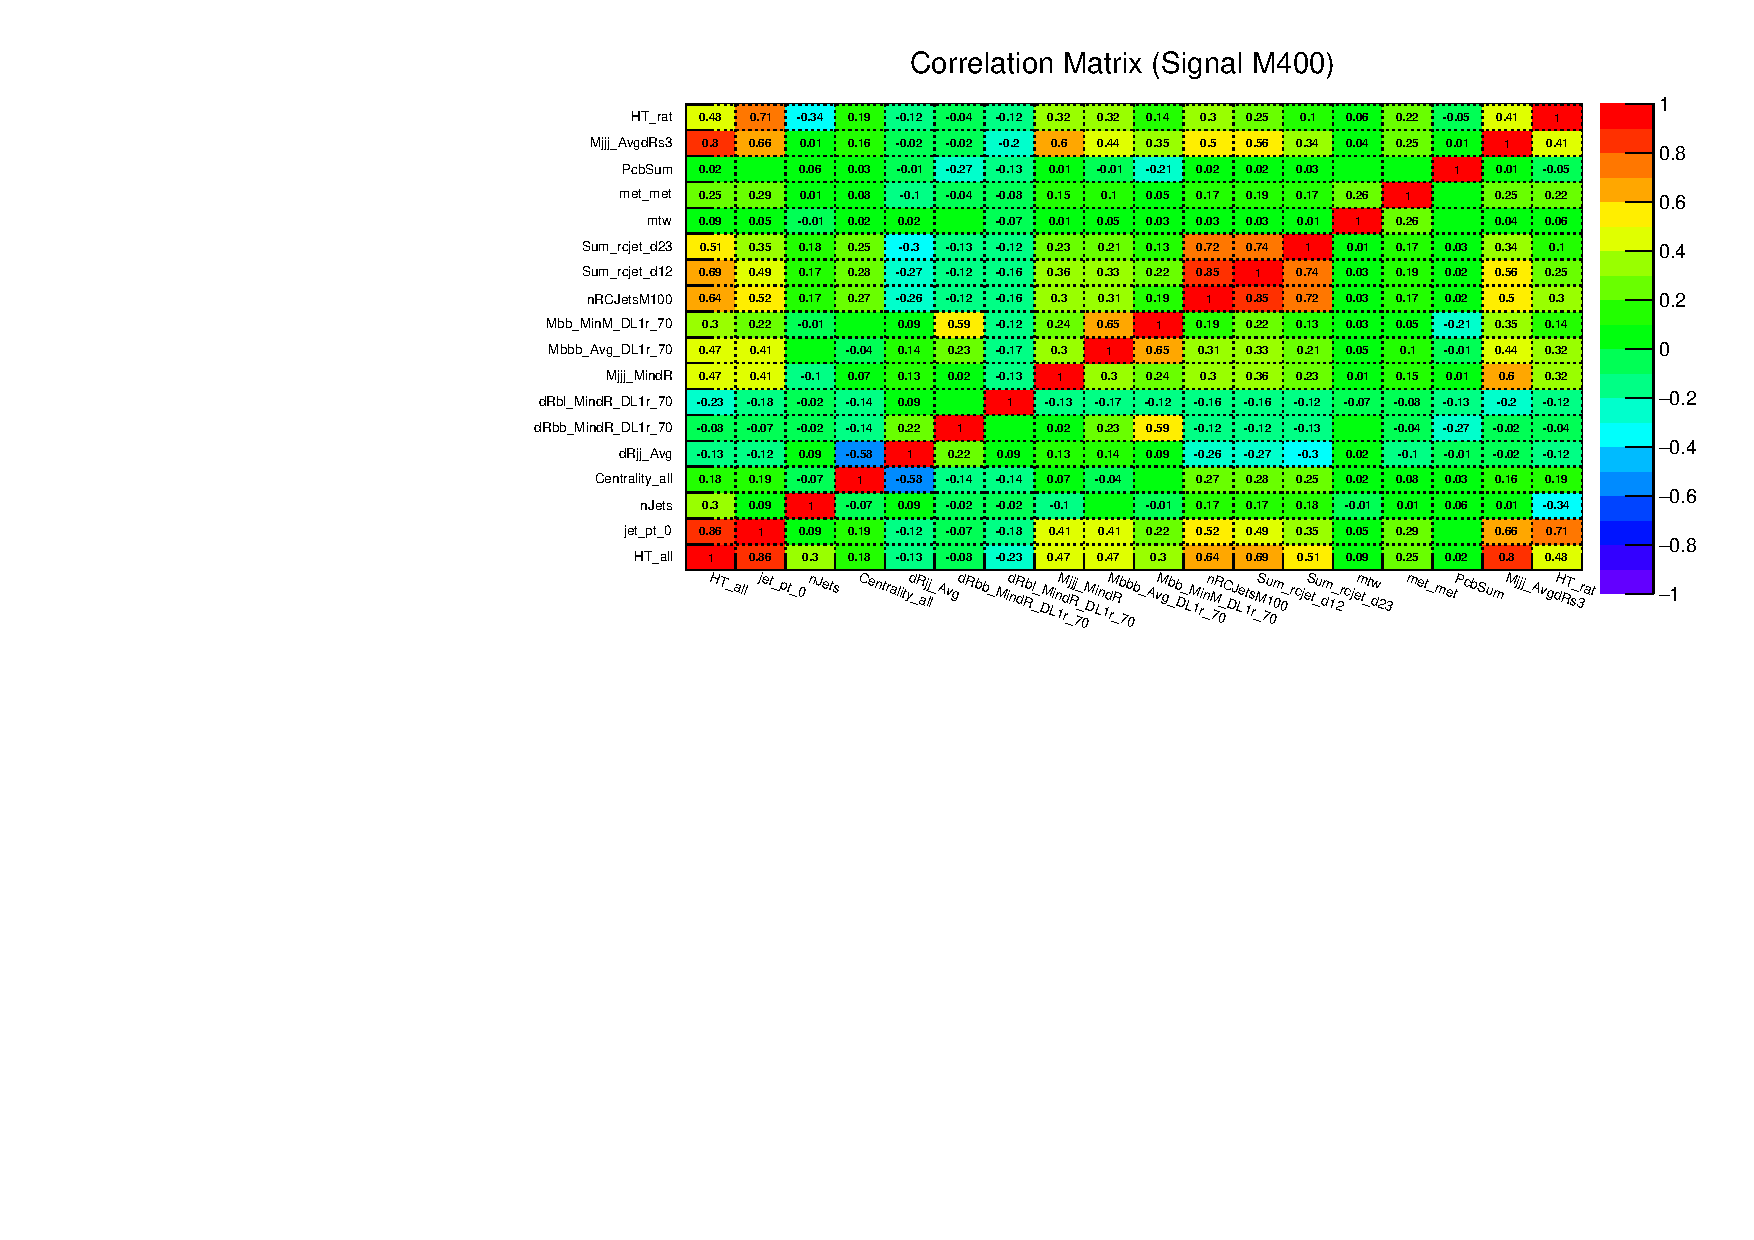
\includegraphics[width=0.55\textwidth]{inputVar_correlation/1L_correlation_m400.pdf}
    \newline
        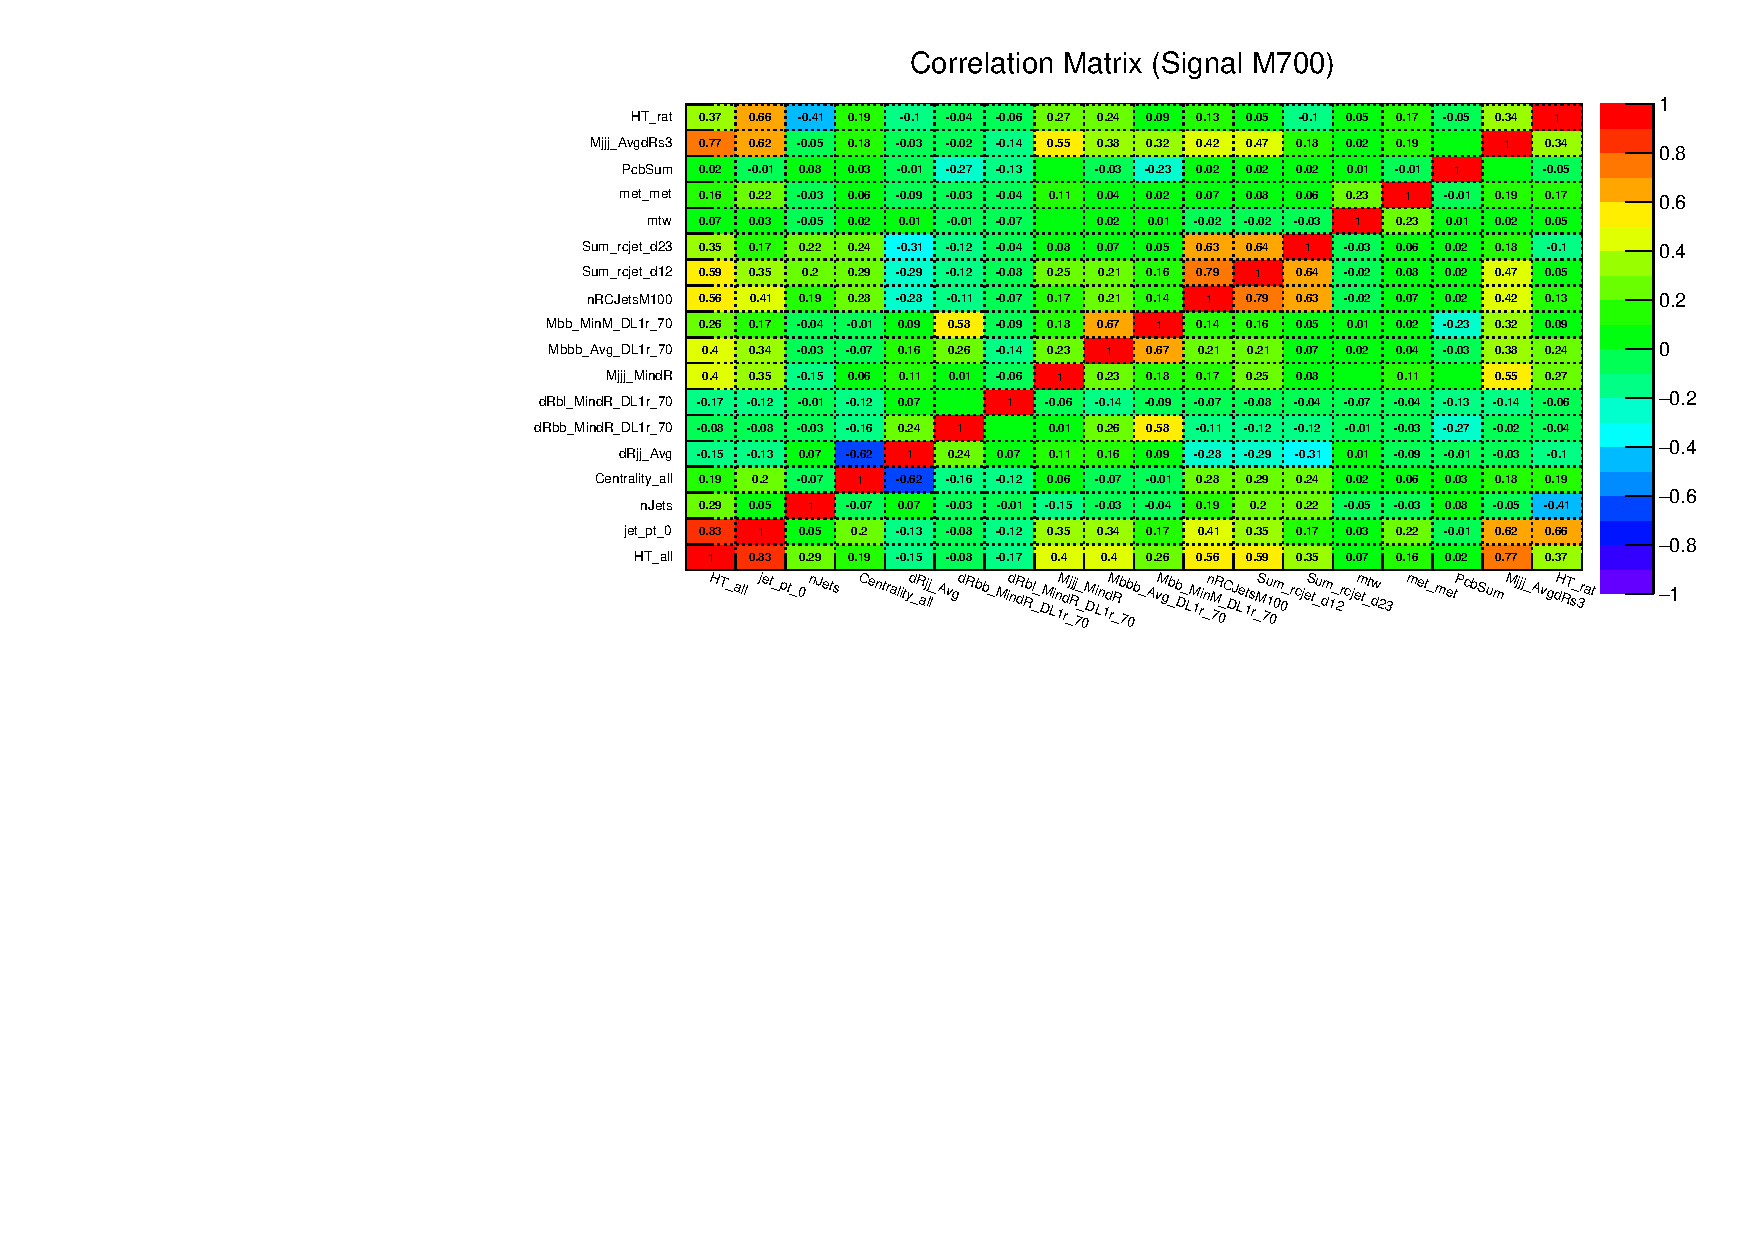
\includegraphics[width=0.55\textwidth]{inputVar_correlation/1L_correlation_m700.pdf}
    \newline    
        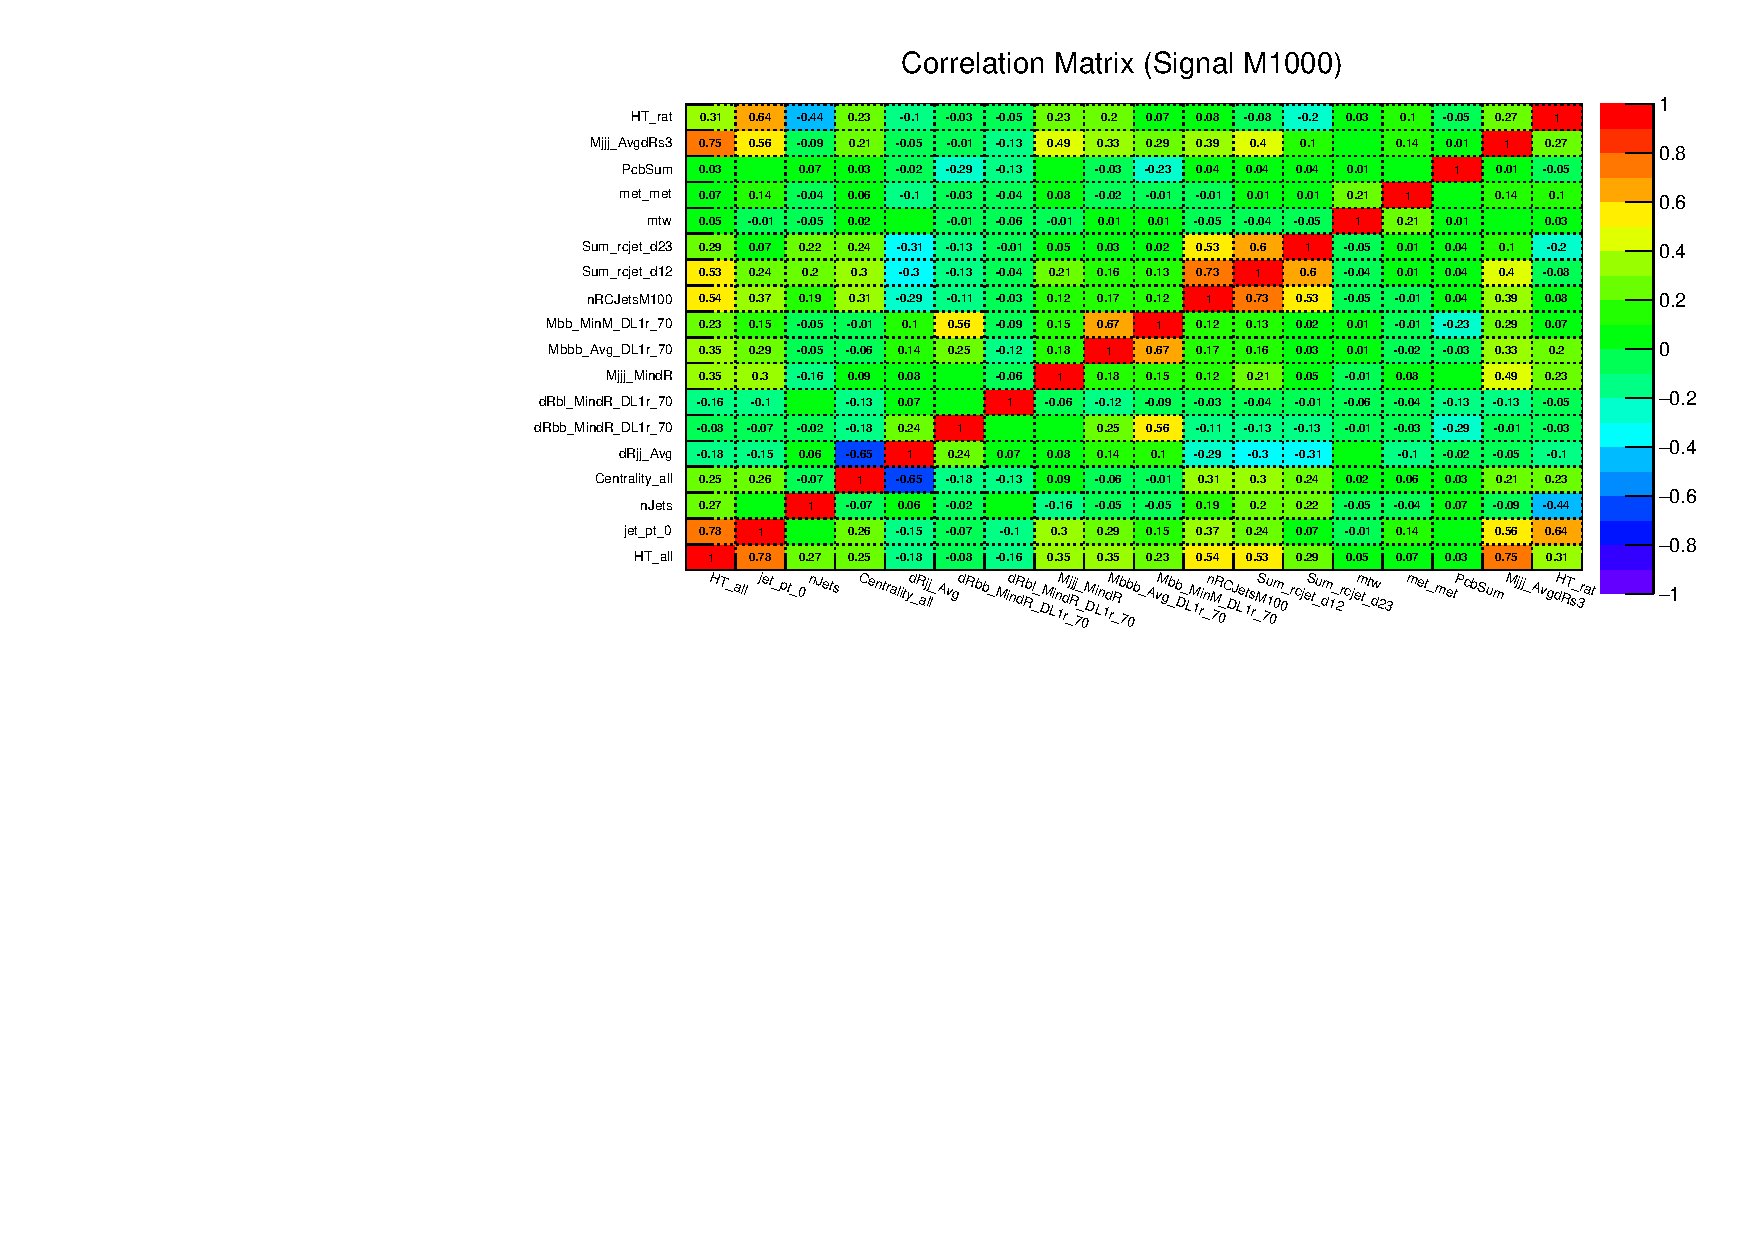
\includegraphics[width=0.55\textwidth]{inputVar_correlation/1L_correlation_m1000.pdf}
    \newline   
    \caption{\label{fig:1L_inputVarCorrelation}The correlation plots of all the input variables in $t\bar{t}$+jets background, and $t\bar{t}H(\rightarrow t\bar{t})$ with BSM Higgs boson mass of 400 GeV, 700 GeV and 1000 GeV in the region of 1L$\geq 9j \geq 3b$. The empty bins correspond to no correlation between variables.}
\end{figure}
%%%%%%%%%

The above input variables have different separation power in the BDT.
The input variables importance indicates the significant of the variables in the BDT.
A simple way to define the feature importance could be an iterative method which is dropping each feature and calculating the Area Under the ROC Curve (AUC) until all features are processed.
It is more convenient to look at the importance in terms of the percentage change:

%%%%Equation: Importance Definition%%%%
\begin{equation}
\mathrm{Imp}[i]\mathrm{=\frac{{AUC}_{ref}-{AUC}_{i}}{\sum_{i}\mid {AUC}_{ref}-{AUC}_{i} \mid}}~,
\end{equation}
%%%%%%%%%%%%%%%%%%%%%%%%%%%%%%%%%%%%%%%
where $\mathrm{Imp}[i]$ is the importance of input variable with index $i$, $\mathrm{AUC_{ref}}$ is the AUC value of the BDT with all input variables and $\mathrm{AUC_{i}}$ is the AUC value of the BDT trained without input variable $i$.
These AUC values are calculated from the BDT with the nominal hyper-parameters which are discussed in the next sub-section.
Figure~\ref{fig:1L_Importance} shows the importance rank of input variables in different signal mass points BDT are not identical.

%%%%Fig: Importance%%%%
\begin{figure}[!htp]\centering
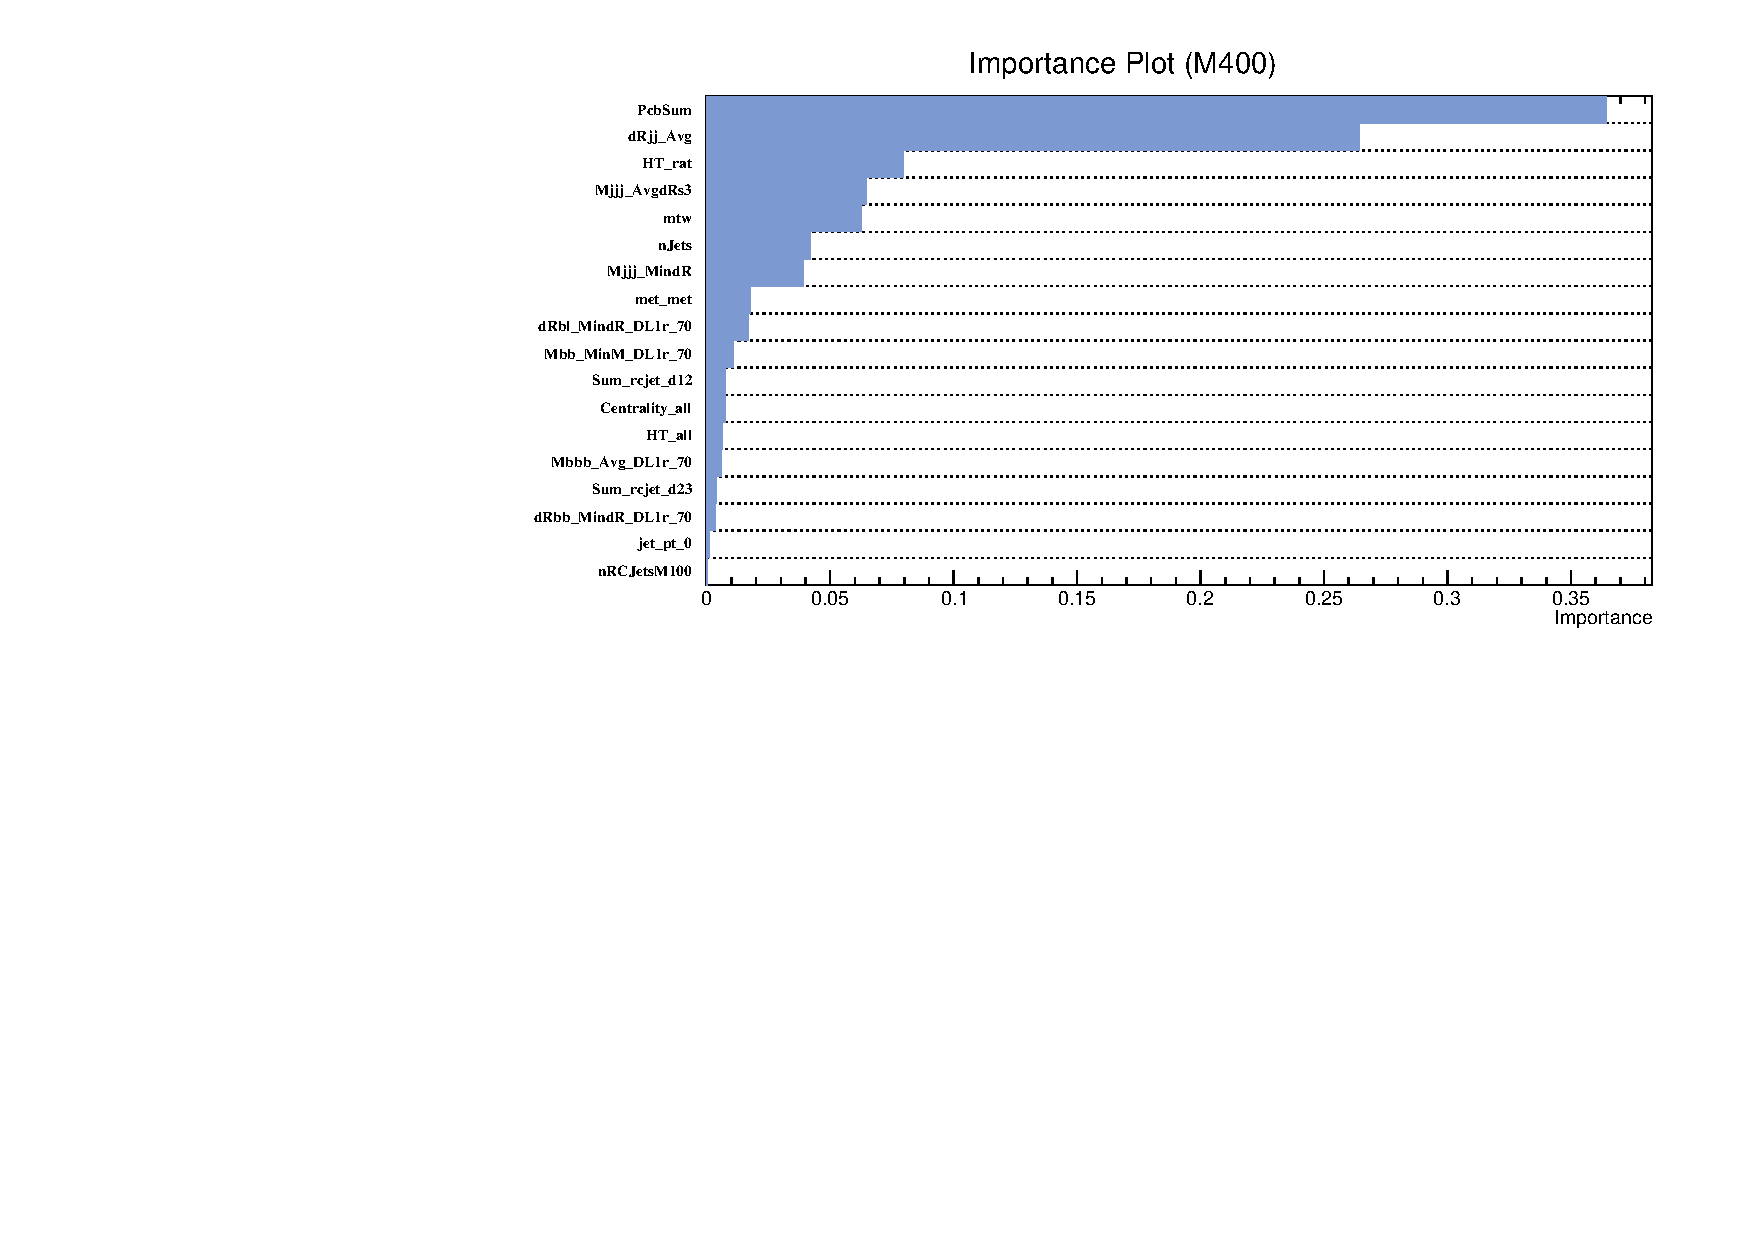
\includegraphics[width=0.75\textwidth]{importance/1L_varImp_M400.pdf}
\\
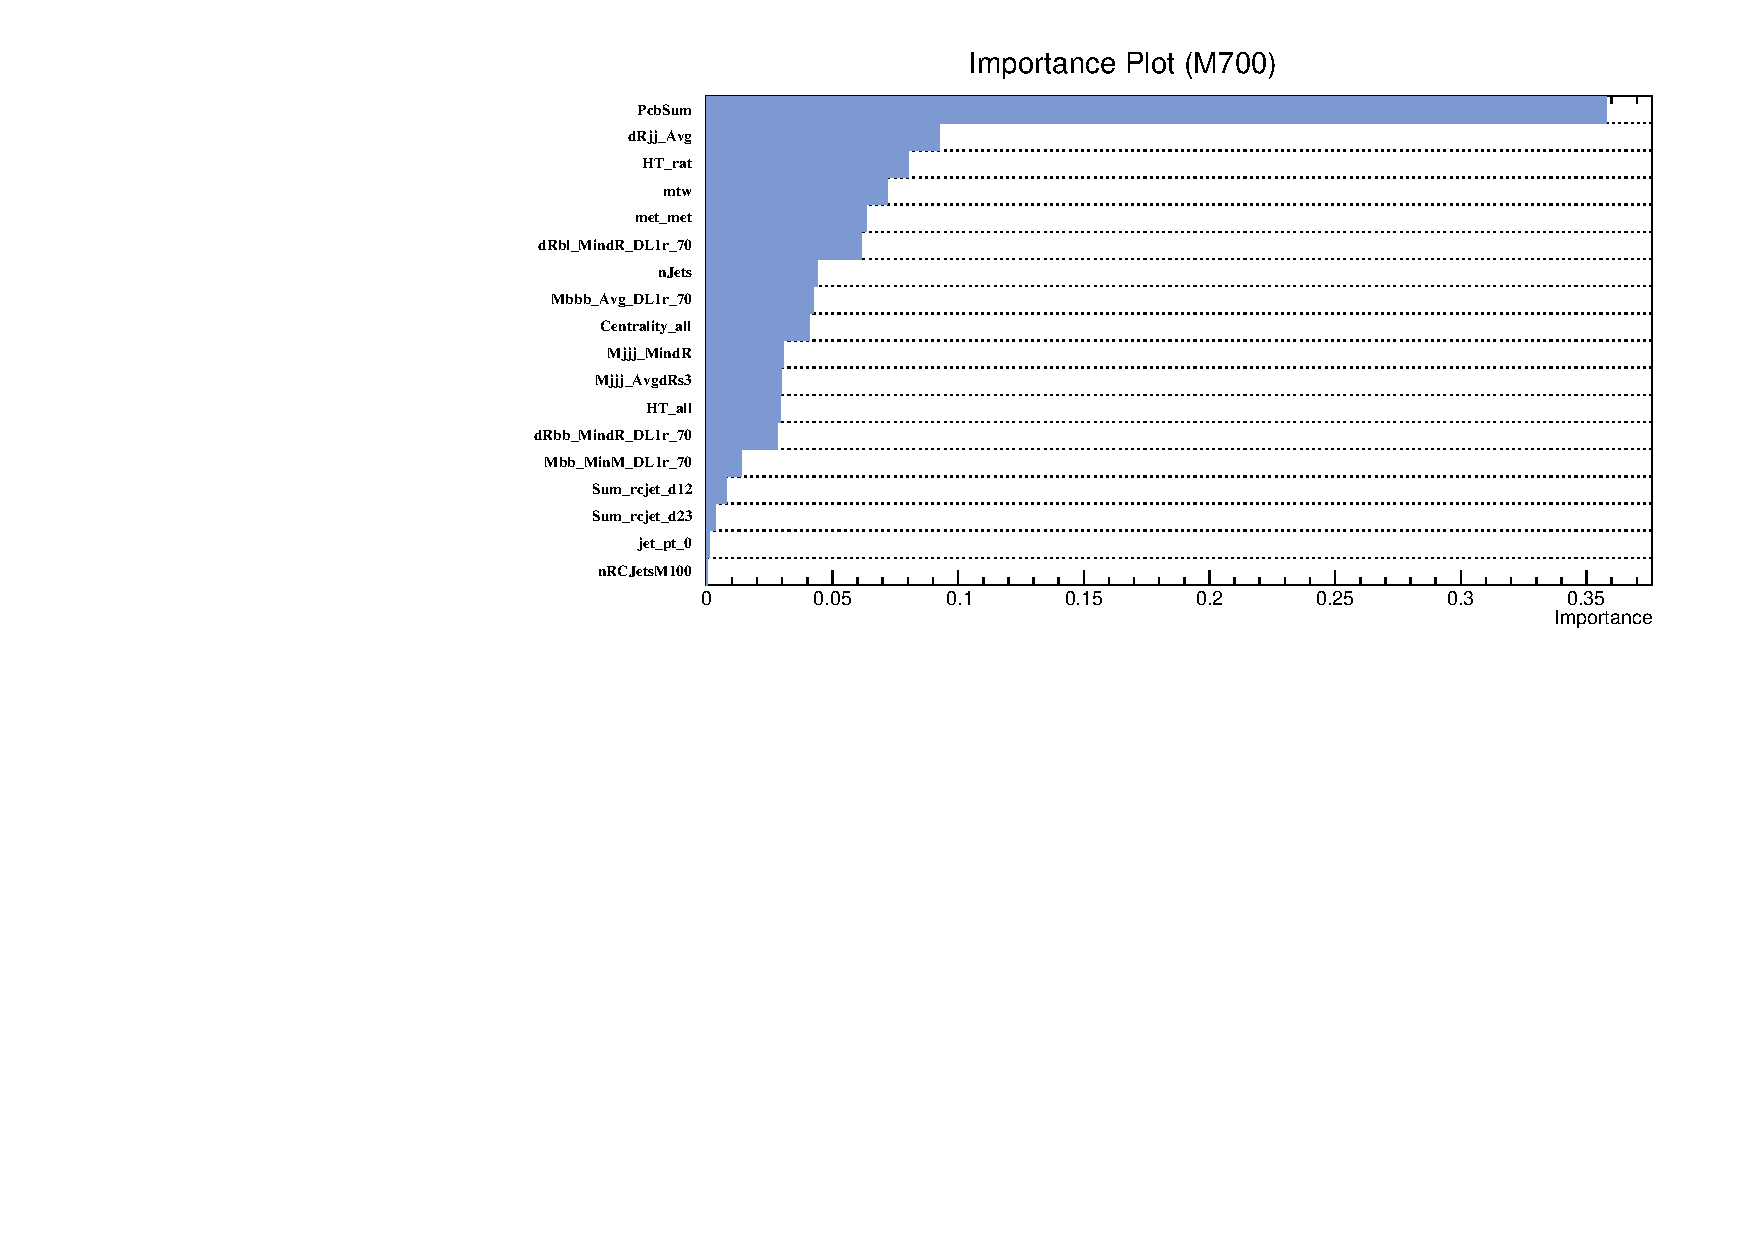
\includegraphics[width=0.75\textwidth]{importance/1L_varImp_M700.pdf}
\\
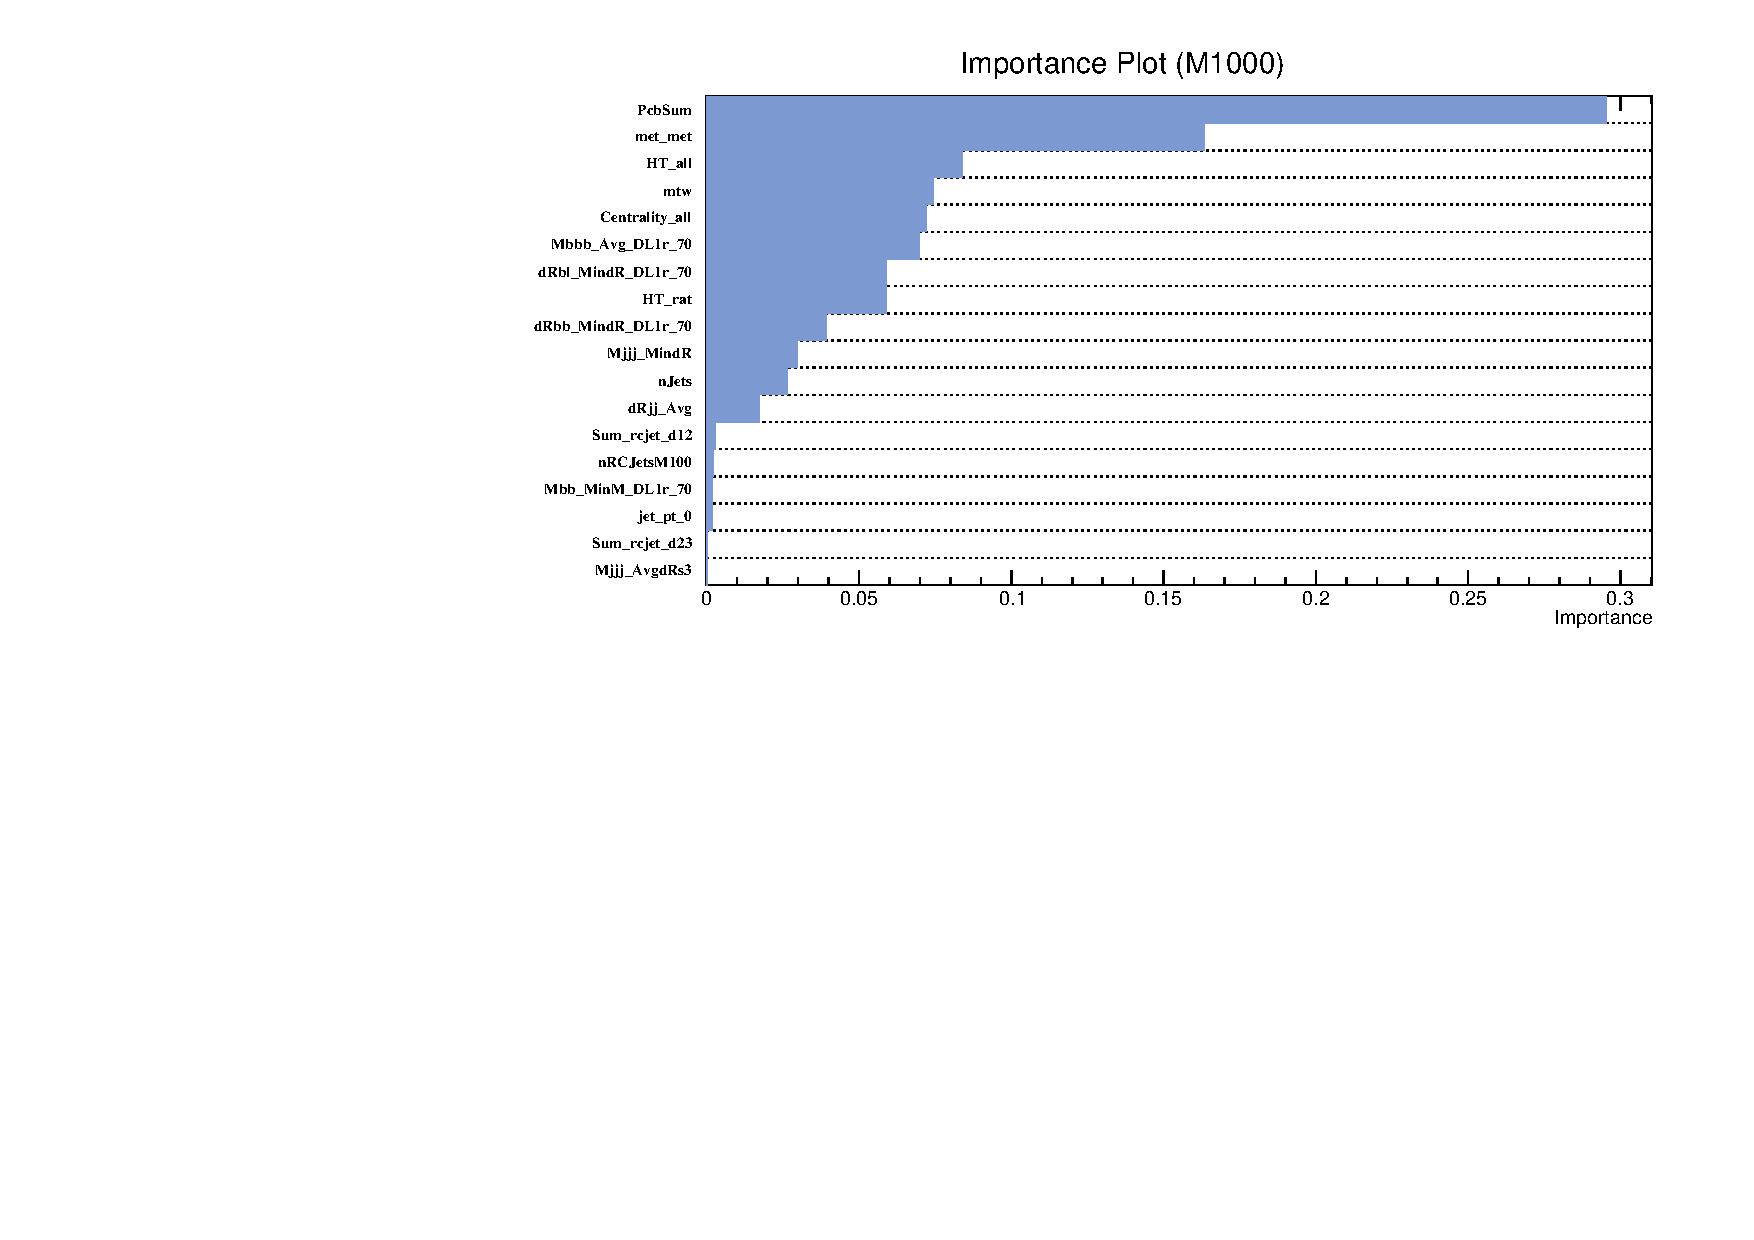
\includegraphics[width=0.75\textwidth]{importance/1L_varImp_M1000.pdf}
\caption{\label{fig:1L_Importance} The importance ranking of input variables in the BDT with BSM Higgs boson mass of (a) $400~GeV$, (b) $700~GeV$ and (c) $1000~GeV$ in $t\bar{t}H(\rightarrow t\bar{t})$ in 1L channel.}

\end{figure}

\begin{figure}[!htp]\centering
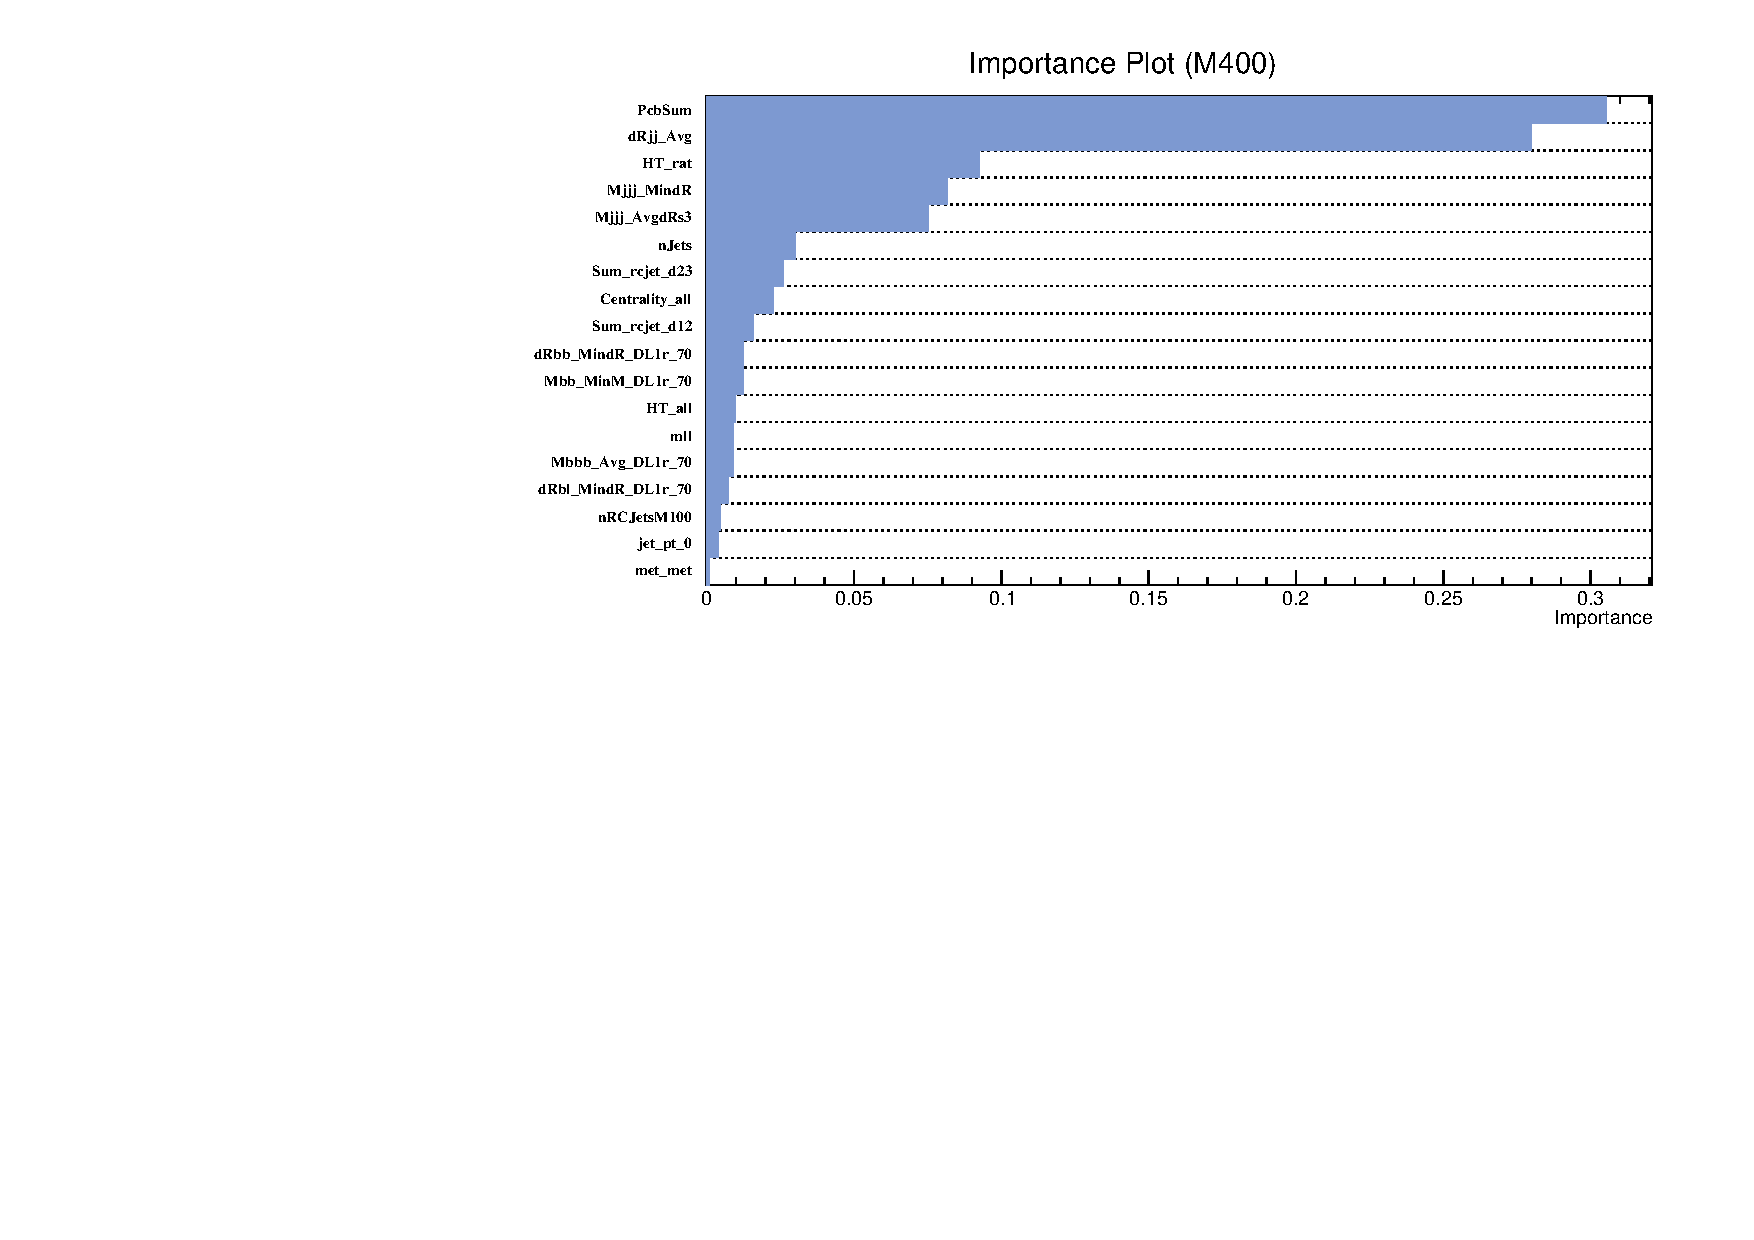
\includegraphics[width=0.75\textwidth]{importance/2LOS_varImp_M400.pdf}
\\
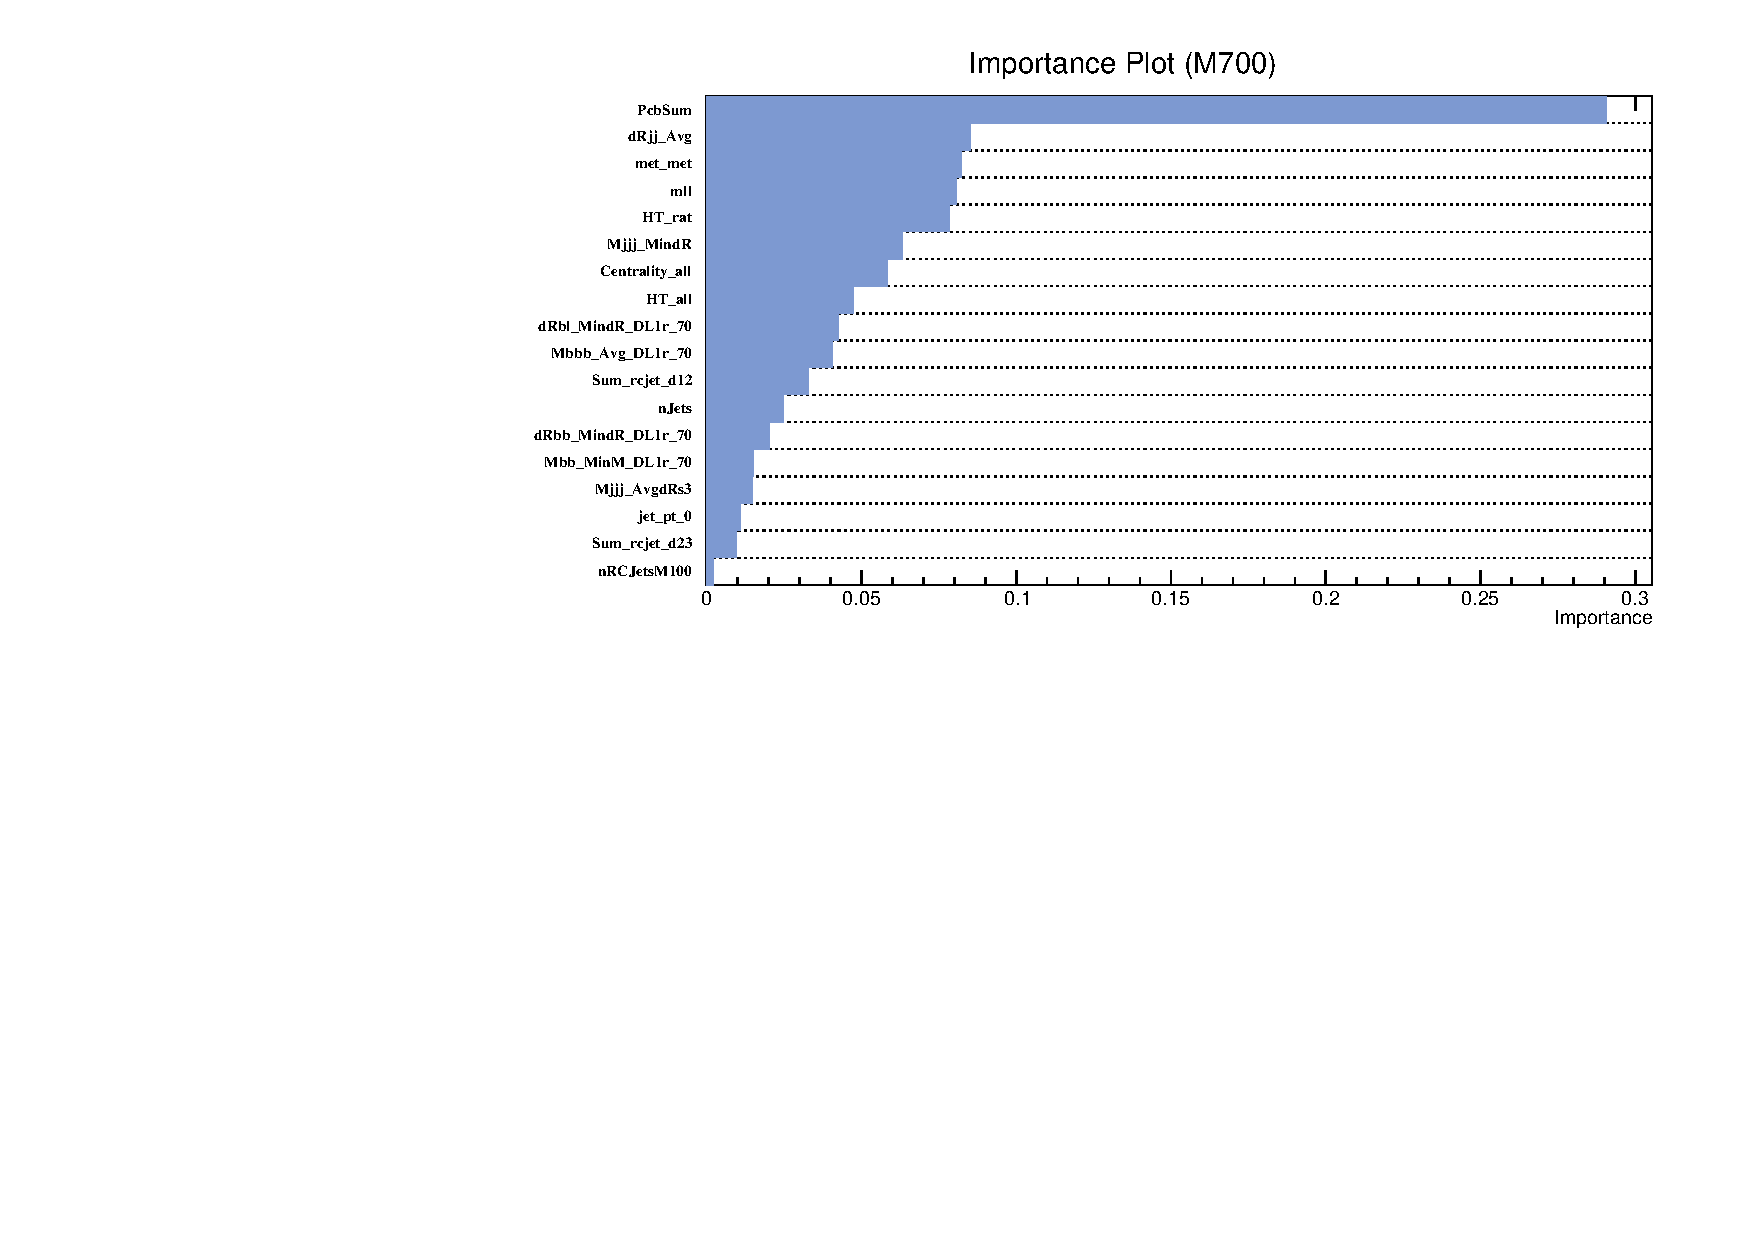
\includegraphics[width=0.75\textwidth]{importance/2LOS_varImp_M700.pdf}
\\
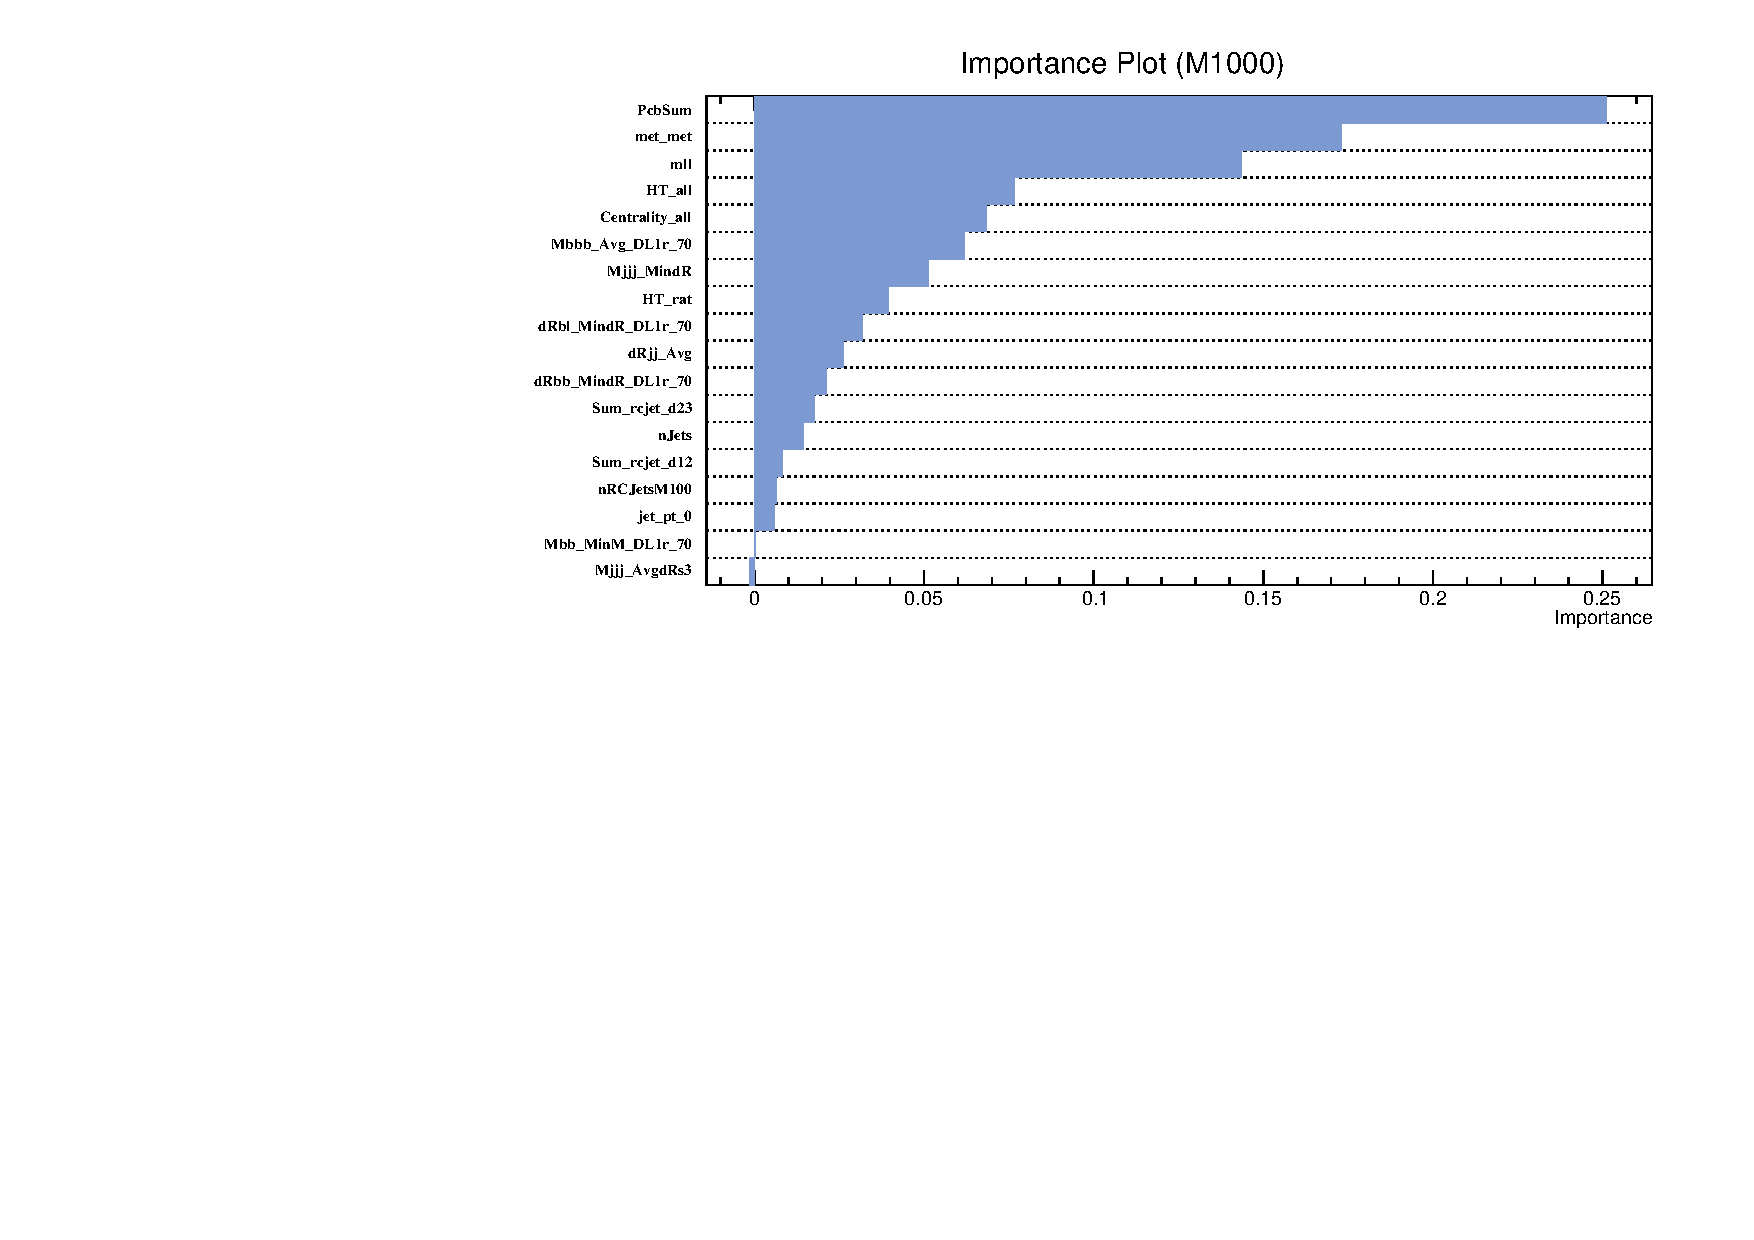
\includegraphics[width=0.75\textwidth]{importance/2LOS_varImp_M1000.pdf}
\caption{\label{fig:2LOS_Importance} The importance ranking of input variables in the BDT with BSM Higgs boson mass of (a) $400~GeV$, (b) $700~GeV$ and (c) $1000~GeV$ in $t\bar{t}H(\rightarrow t\bar{t})$ in 2LOS channel.}

\end{figure}
%%%%%%%%%%%%%%%%%%%%%%%%%%%%

%%%%Table: BDT Variable Rank %%%%
\begin{table}[!htp]
    \centering
\resizebox*{\textwidth}{!}{
    \begin{tabular}{|c||c|c|c||c|c|c||c|c|c|}
        \hline
        &\multicolumn{3}{c|}{M400} & \multicolumn{3}{c|}{M700} & \multicolumn{3}{c|}{M1000}\\
        \hline \hline
        Variable & AUC reduction & Separation & TMVA Importance & AUC reduction & Separation & TMVA Importance & AUC reduction & Separation & TMVA Importance \\
        \hline
        $H_{T}$ & 13 & 9 & 10 & 12 & 1 & 12 & 3 & 1 & 1 \\
        $\sum_{i} {p_{T}}_{i}/ \sum_{i} E_{i}$ & 12 & 3 & 9 & 9 & 9 & 5 & 5 & 10 & 3 \\
        $N_{jets}$ & 6 & 4 & 14 & 7 & 6 & 15 & 11 & 9 & 16 \\
        ${p_{T}}_{0}$ & 17 & 15 & 13 & 17 & 10 & 16 & 16 & 5 & 14 \\
        $\Delta R^{avg}_{jj}$ & 2 & 2 & 1 & 2 & 12 & 2 & 12 & 14 & 11 \\
        $M^{min. \Delta R}_{jjj}$ & 7 & 11 & 5 & 10 & 11 & 11 & 10 & 8 & 10 \\
        $M^{\Delta R<3}_{jjj}$ & 4 & 5 & 4 & 11 & 2 & 9 & 18 & 2 & 12 \\
        $\sum^{3}_{i=0}{p_{T}}_{i} / \sum_{i\geq 4} {p_{T}}_{i}$ & 3 & 6 & 2 & 3 & 16 & 1 & 8 & 17 & 2 \\
        $\Delta R^{min}_{bl}$ & 9 & 18 & 8 & 6 & 18 & 4 & 7 & 16 & 5 \\
        $\Delta R^{min}_{bb}$ & 16 & 14 & 6 & 13 & 17 & 10 & 9 & 18 & 8 \\
        $M^{avg}_{bbb}$ & 14 & 12 & 12 & 8 & 8 & 6 & 6 & 6 & 7 \\
        $M^{min}_{bb}$ & 10 & 16 & 11 & 14 & 13 & 13 & 15 & 12 & 17 \\
        $\sum^{i<4}_{i=0} {pcb}_{i}$ & 1 & 1 & 3 & 1 & 5 & 3 & 1 & 11 & 6 \\
        $N_{RC100}$ & 18 & 10 & 18 & 18 & 4 & 18 & 14 & 4 & 18 \\
        $\sum d_{12}$ & 11 & 7 & 16 & 15 & 3 & 14 & 13 & 3 & 13 \\
        $\sum d_{23}$ & 15 & 8 & 17 & 16 & 7 & 17 & 17 & 7 & 15 \\
        $E^{miss}_{T}$ & 8 & 17 & 15 & 5 & 14 & 8 & 2 & 13 & 4 \\
        $m_{T}(\ell,E^{miss}_{T})$ & 5 & 13 & 7 & 4 & 15 & 7 & 4 & 15 & 9 \\
        \hline
    \end{tabular}
}
\caption{BDT input variables ranking based on different method in 1L channel. \label{tab:variableRank_1L}}
\end{table}

%%%%%%%%%%%%%%%%%%%%%%%%%%%%%%%%%

%%%%Next Sub-section%%%%
\subsubsection{Hyper-parameters}

The BDT has several hyper-parameters which are relevant to this study:

\begin{itemize}
\item Boosting algorithm
\item Number of trees (Number of boosting iteration) (NTrees)
\item Learning rate to control the sample overfitting ($\eta$)
\item Bagged sample fraction which creates a sub-sample with certain fraction in training sample including replacement and are used in each boosting iteration  
\item Separation method of node splitting during tree training
\item Number of gird points in input variable range used to represent the optimal cut in node splitting (nCuts)
\item Maximum tree depth allowed (MaxDepth)
\end{itemize}

The hyper-parameters setup are optimized by scanning the average AUC-value among all the signal mass points in the testing BDT and the average AUC difference between training and testing BDT with different hyper-parameters combination.
A high AUC-value implies a high separation between signal and background while a low AUC difference indicates no overtraining.

In the optimization study, the boosting algorithm is fixed to Gradient Boost with bagging fraction 60\%.
The separation method in a node splitting is chosen to be Gini Index.
The remaining parameters are scanned in 300 combinations with different NTrees, $\eta$, nCuts and MaxDepth, as shown in Table~\ref{tab:hyperParameterScan}.
Figure~\ref{fig:1LHyperParaT600} and Figure~\ref{fig:1LHyperParaT1000} show the results from the hyper-parameters scan at NTrees$=600$ and $1000$ respectively in 1L$\geq 9j\geq 3b$ region.
Since no big improvement on the sensitivity is found after the hyper-parameters optimization, the BDT hyper-parameters in this analysis are chosen to be the same as those in the SM4t studies:

\begin{itemize}
\item Number of trees: 600
\item Boosting: Gradient with bagging (sample fraction of 0.6)
\item Learning-rate: 0.05
\item Loss function: GiniIndex
\item Number of scanned cuts: 30
\item Maximum tree depth: 2
\end{itemize}

%%%%Table: Hyperparameter Scan%%%%
\begin{table}[!htp]
    \centering
    \begin{tabular}{|c|c|c|c|}
        \hline
        NTrees & $\eta$ & nCuts & MaxDepth \\
        \hline
        200 & 0.01 & 25 & 2\\
        400 & 0.02 & 30 & 3\\
        600 & 0.05 & 35 & 4\\
        800 & 0.10 &    & \\
        1000 & 0.20 &   &  \\
        \hline
    \end{tabular}
\caption{Different hyper-parameters scanning points. \label{tab:hyperParameterScan}}
\end{table}
%%%%%%%%%%%%%%%%%%%%%%%%%%%%%%%%%

%%%%Figure : Hyperparameter Scan T600 %%%%
\begin{figure}[!htp]
    \centering
        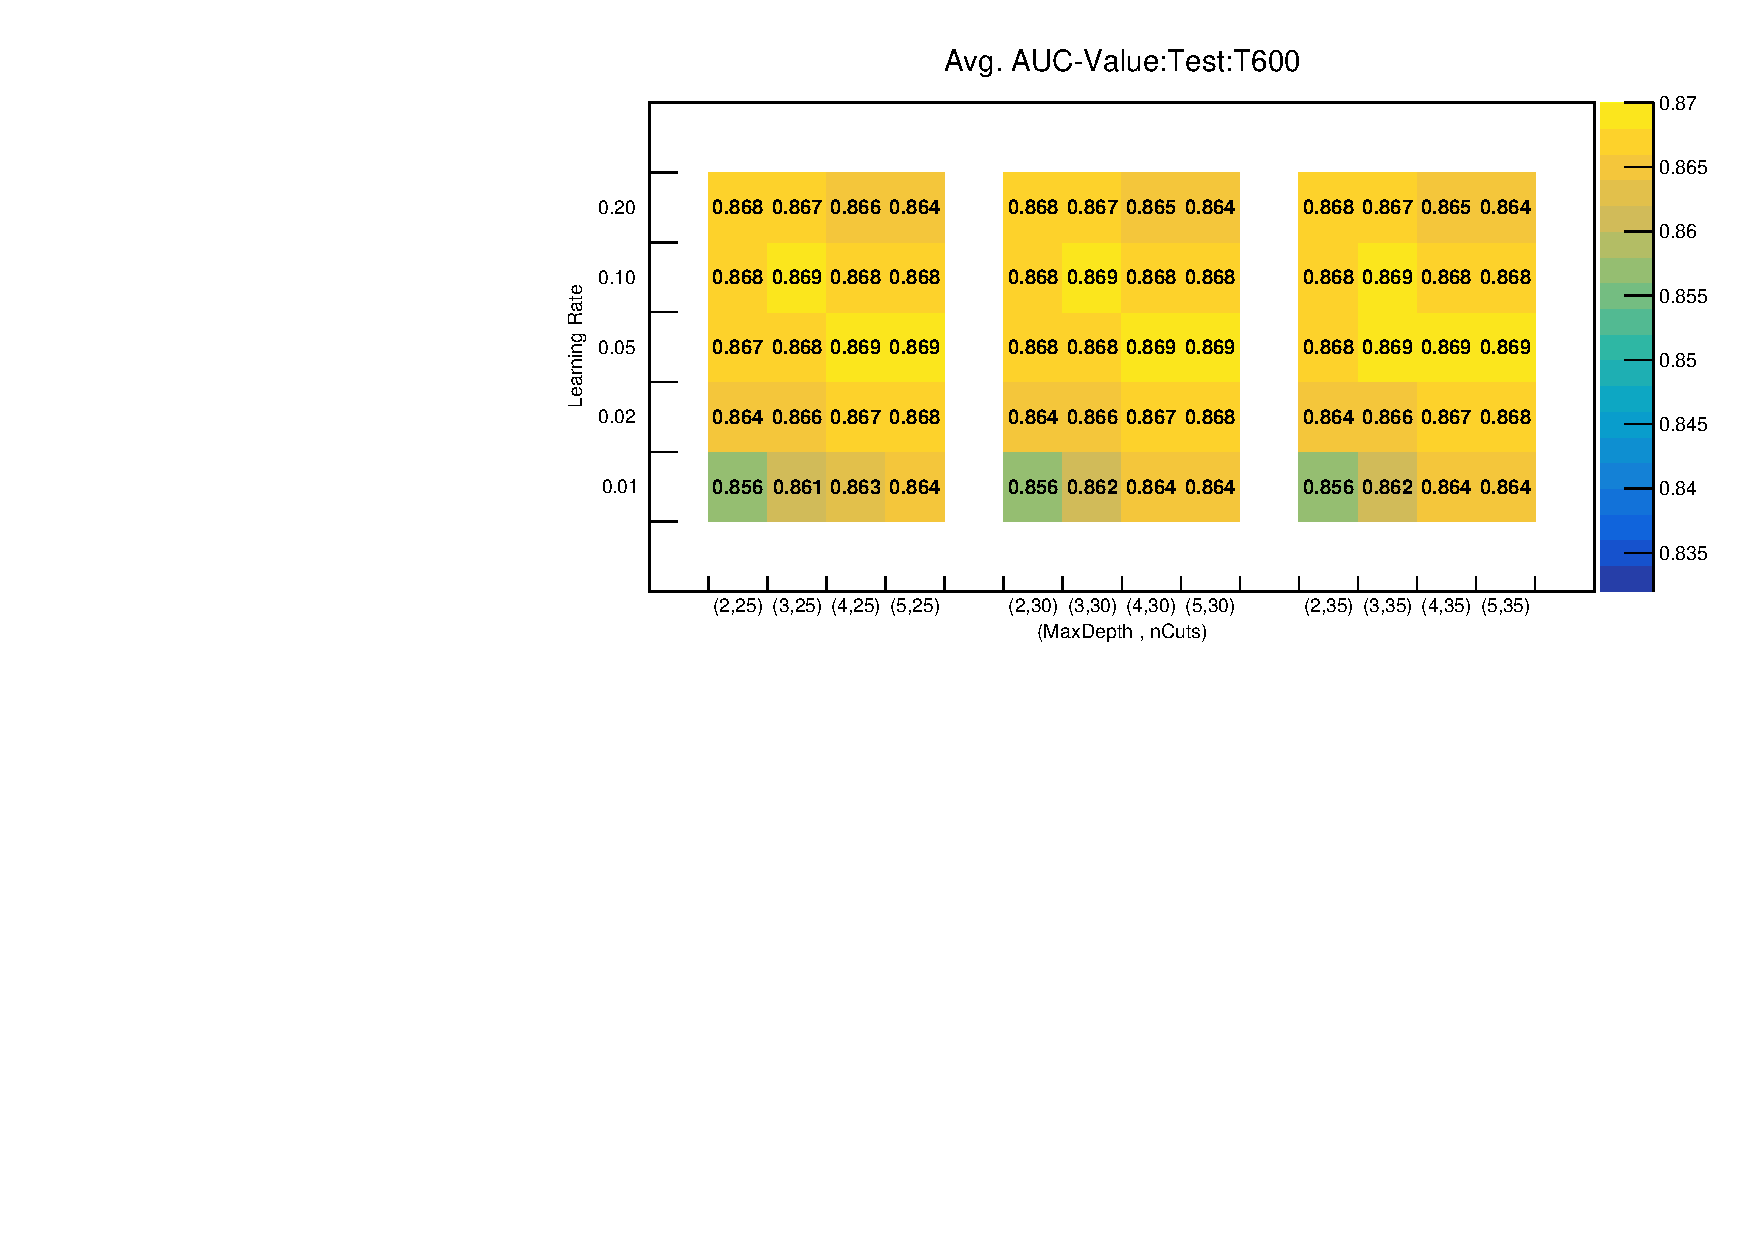
\includegraphics[width=0.55\textwidth]{hyperParameter/T600_test_1L.pdf}
        \subcaption{Average AUC Value of Testing with NTrees 600}
        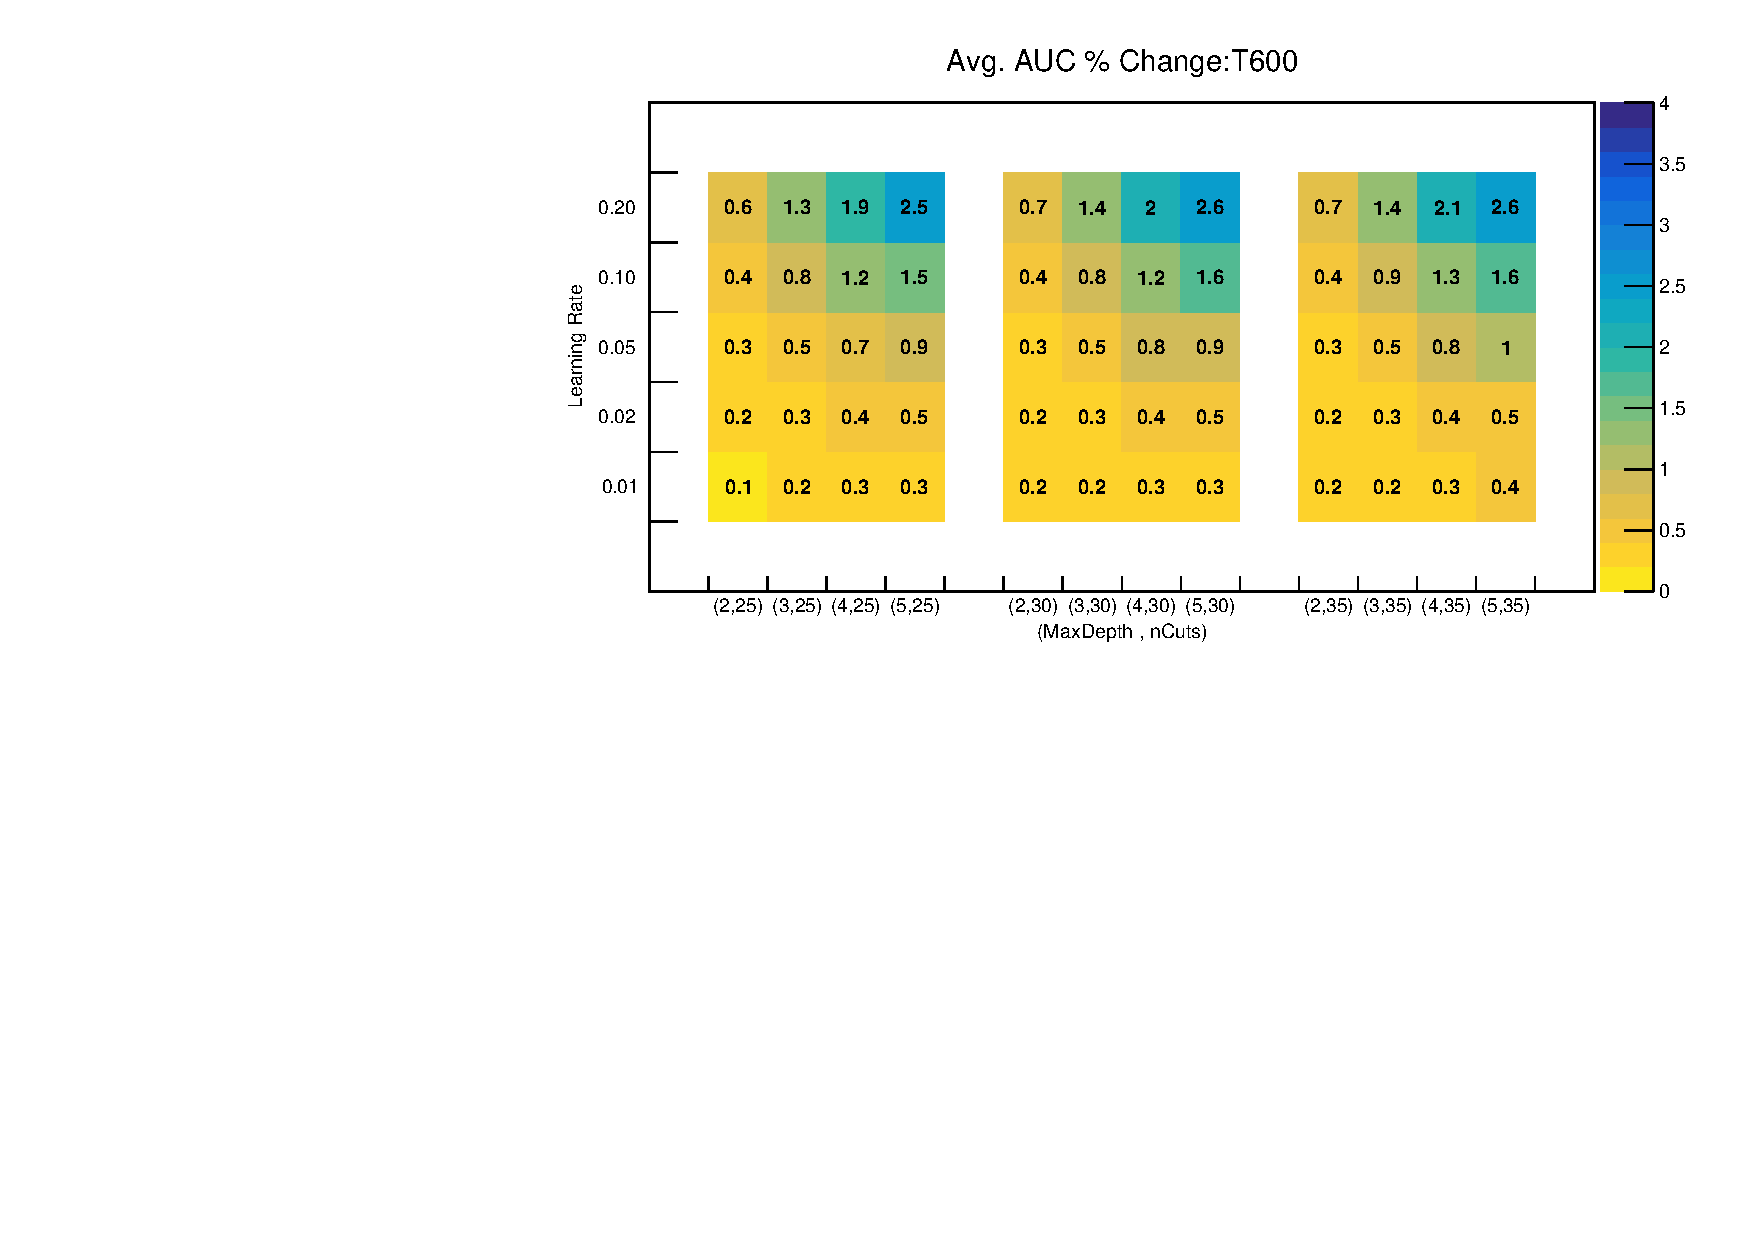
\includegraphics[width=0.55\textwidth]{hyperParameter/T600_val_1L.pdf}
        \subcaption{Average AUC \% Change with NTrees 600}
    \caption{\label{fig:1LHyperParaT600}Hyper-parameter scan at learning-rate, maximum tree depth and the number of cuts in the input variables by fixing the number of trees into 600. Figure (a) gives the average AUC-value in the test BDT with different hyper-parameter setup while figure (b) gives the AUC \% difference between train and test BDT, which is defined as $\mathrm{(AUC^{avg}_{train}-AUC^{avg}_{test})/AUC^{avg}_{train}}\times 100$. The scan is performed in 1L$\geq 9j \geq 3b$ region}
\end{figure}    
%%%%%%%%%%%%%%%%%%%%%%%%%%%%%%%%%%%%%%%%%    

%%%%Figure : Hyperparameter Scan T600 %%%%
\begin{figure}[!htp]
    \centering
%    \subfloat[Average AUC Value of Testing with NTrees 1000]{
        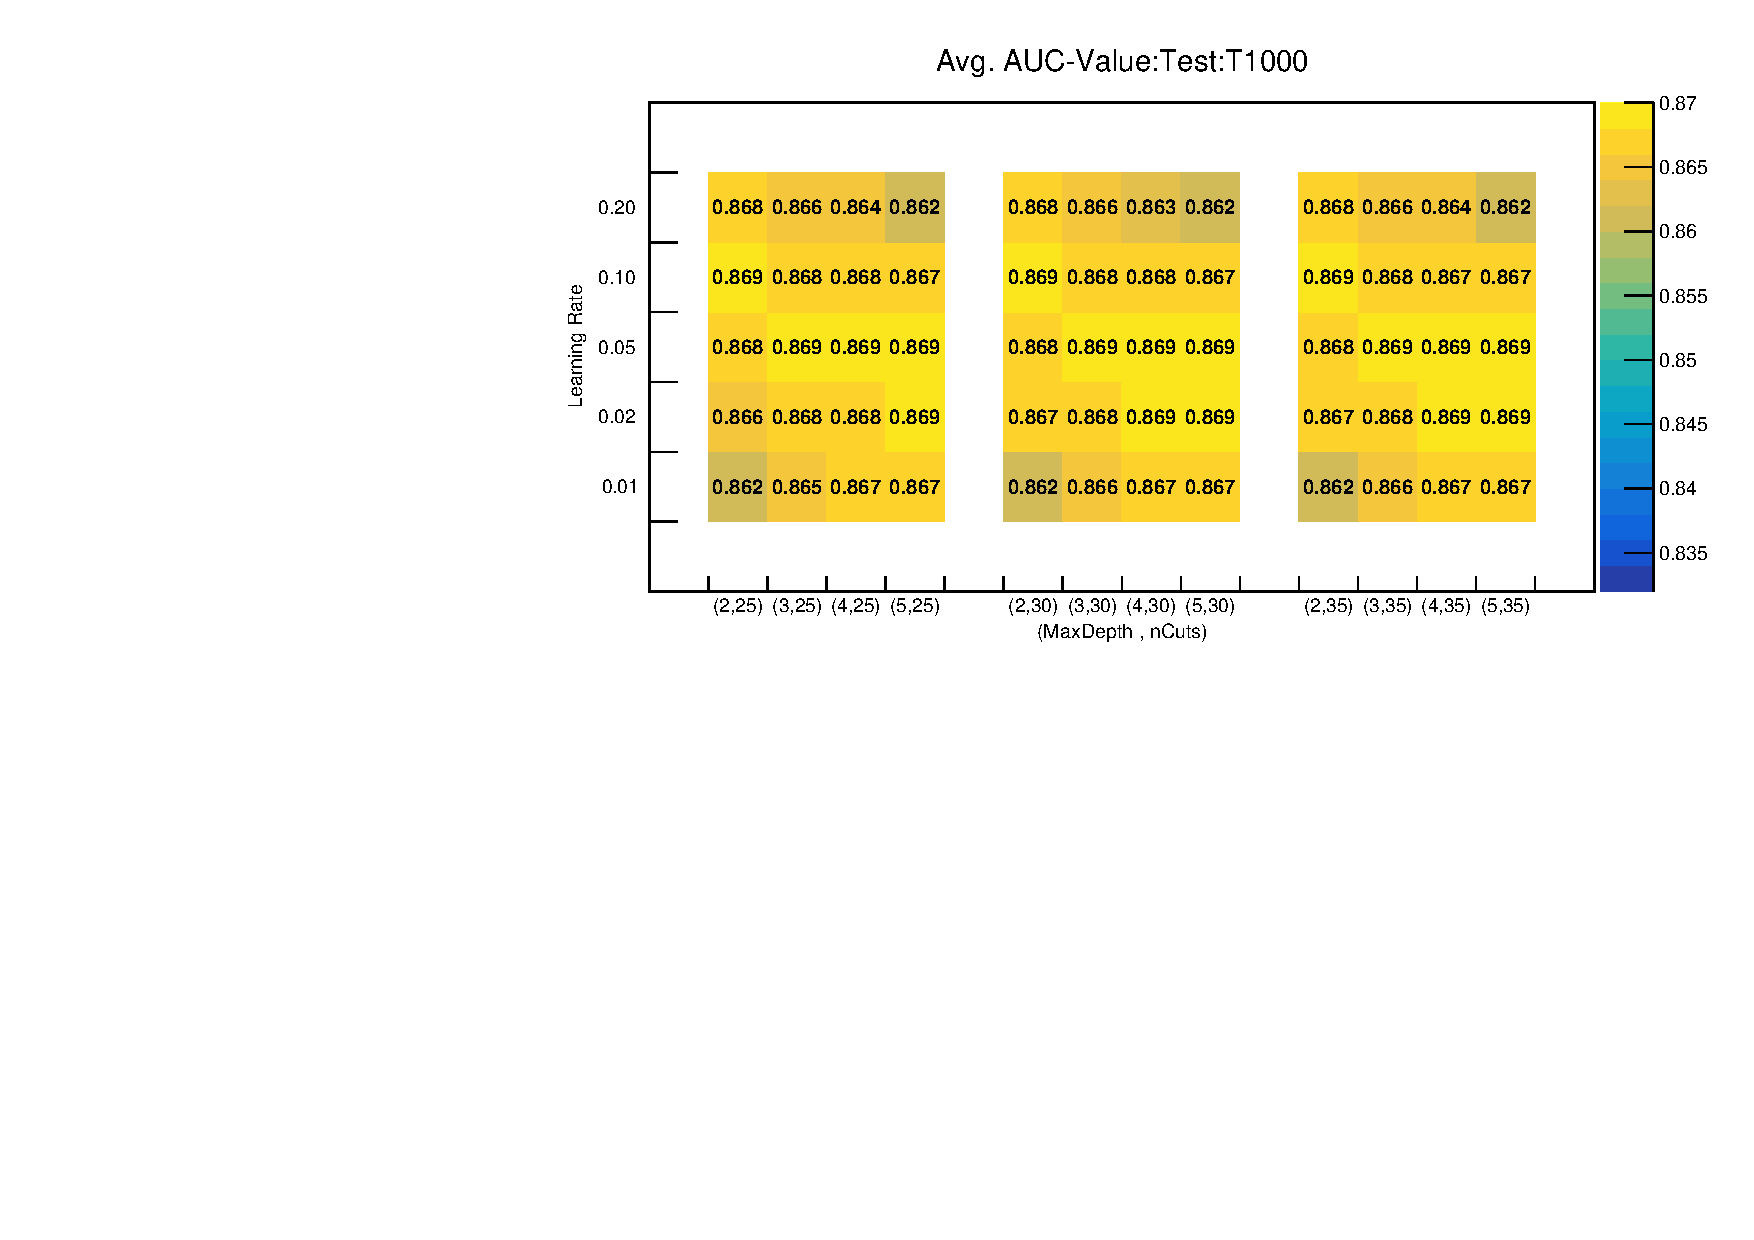
\includegraphics[width=0.55\textwidth]{hyperParameter/T1000_test_1L.pdf}
%    }
%    \subfloat[Average AUC \% Change with NTrees 1000]{
        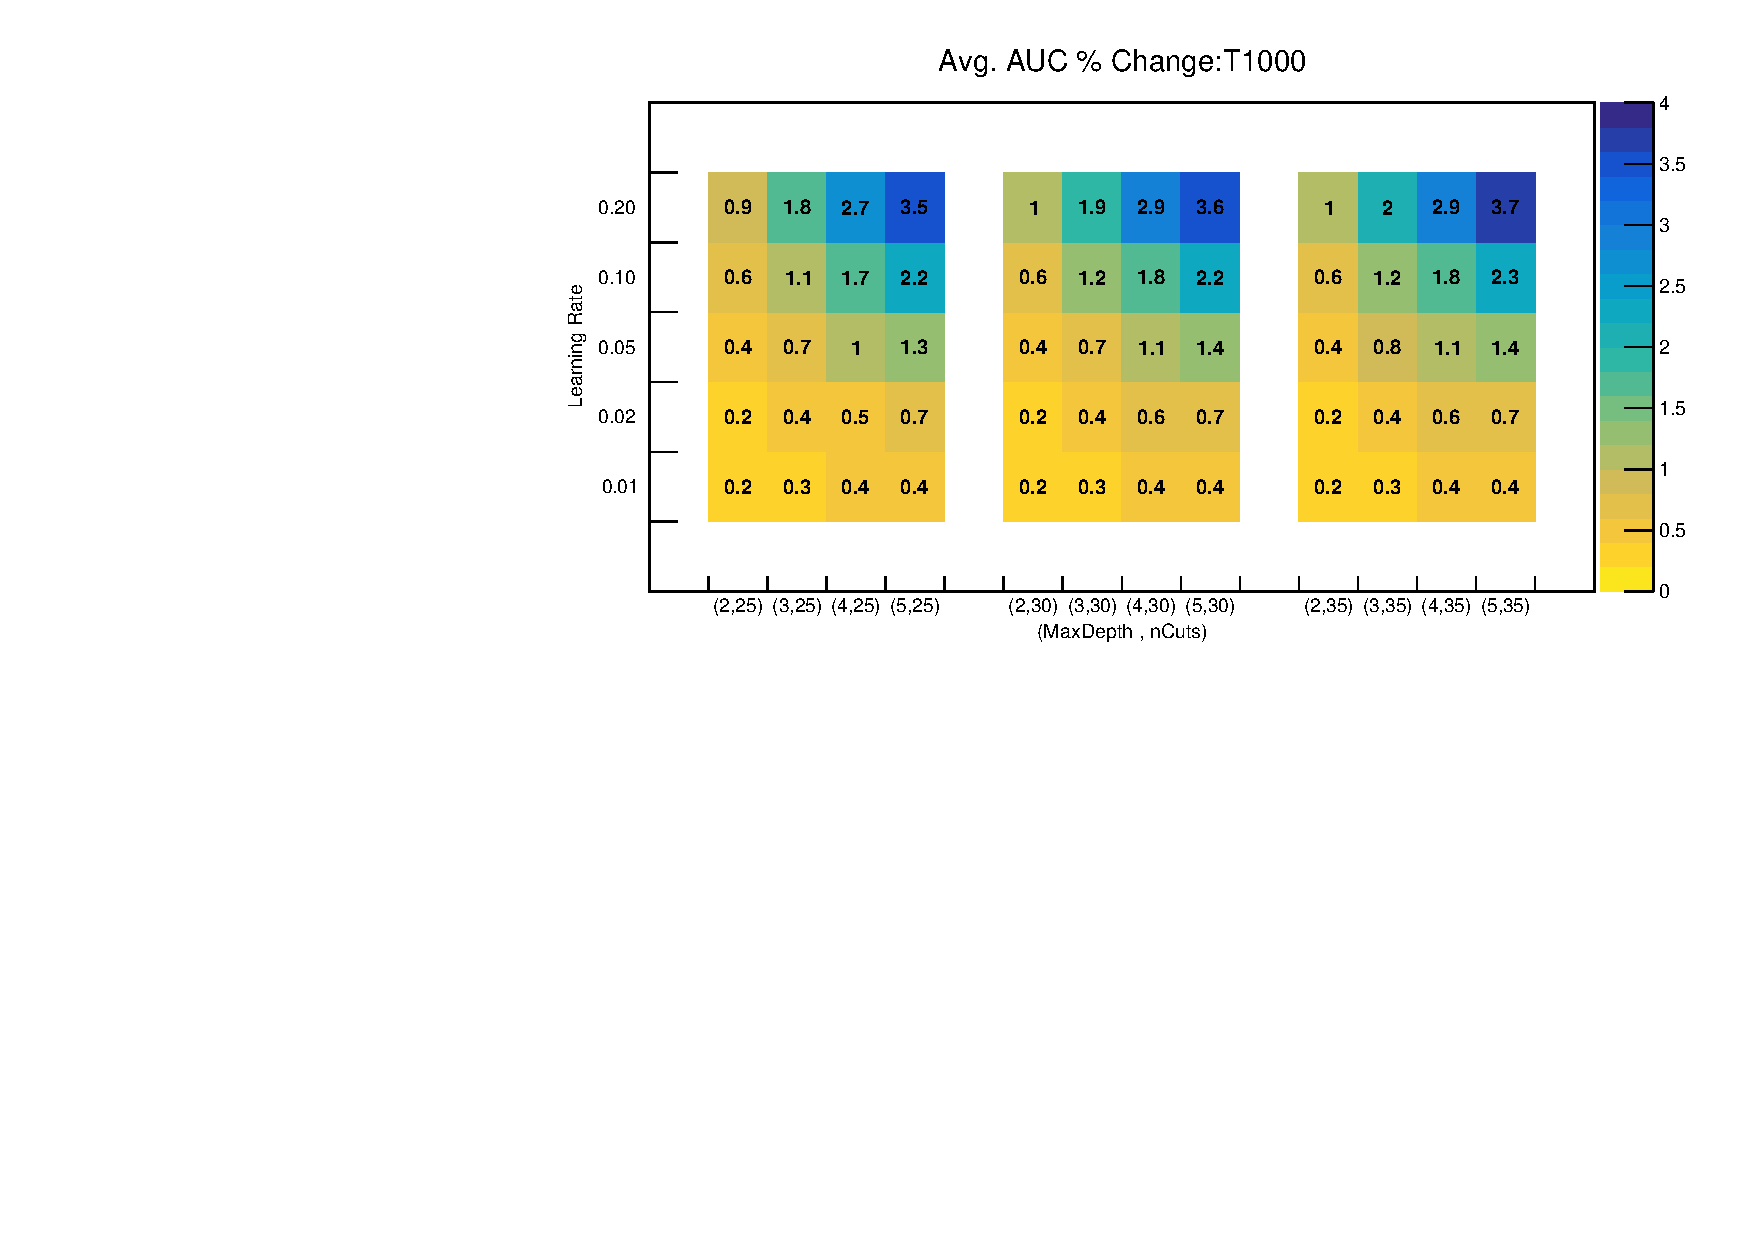
\includegraphics[width=0.55\textwidth]{hyperParameter/T1000_val_1L.pdf}
%    }
    \caption{\label{fig:1LHyperParaT1000}Hyper-parameter scan at learning-rate, maximum tree depth and the number of cuts in the input variables by fixing the number of trees into 1000. Figure (a) gives the average AUC-value in the test BDT with different hyper-parameter setup while figure (b) gives the AUC \% difference between train and test BDT, which is defined as $\mathrm{(AUC^{avg}_{train}-AUC^{avg}_{test})/AUC^{avg}_{train}}\times 100$. The scan is performed in 1L$\geq 9j \geq 3b$ region}
\end{figure}    
%%%%%%%%%%%%%%%%%%%%%%%%%%%%%%%%%%%%%%%%% 

%%%%Next Sub-section%%%%
\subsubsection{Performance of BDT}
The BDT performance is evaluated by the AUC value of the ROC curve and the overtraing check.
Overtraining is checked by comparing the AUC value between the training and the testing BDT in the combination of even and odd samples.
The AUC value increases with the signal mass points used in the BDT training, from $0.81$ for M400 to $0.91$ for M1000 while the deviations of testing BDT AUC value from the training one is within $0.6$ \% for all the signal mass points in the region of 1L$\geq 9j \geq 3b$.
Figure~\ref{fig:1Lge9jge3bBDT} provides the distribution of BDT and ROC of signal mass points M400, M700 and M1000 in 1L$\geq 9j\geq 3b$ region.
A trend of AUC value in the signal mass points is shown in Figure~\ref{fig:AUC_perMP}, that the AUC value increases with the signal mass point because the separation of most of the variables between signal and background increases with the BSM Higgs boson mass.
 
%%%%Fig: 1L BDT and ROC%%%%
\begin{figure}[!htp]\centering
   \begin{subfigure}[t]{0.49\textwidth}
        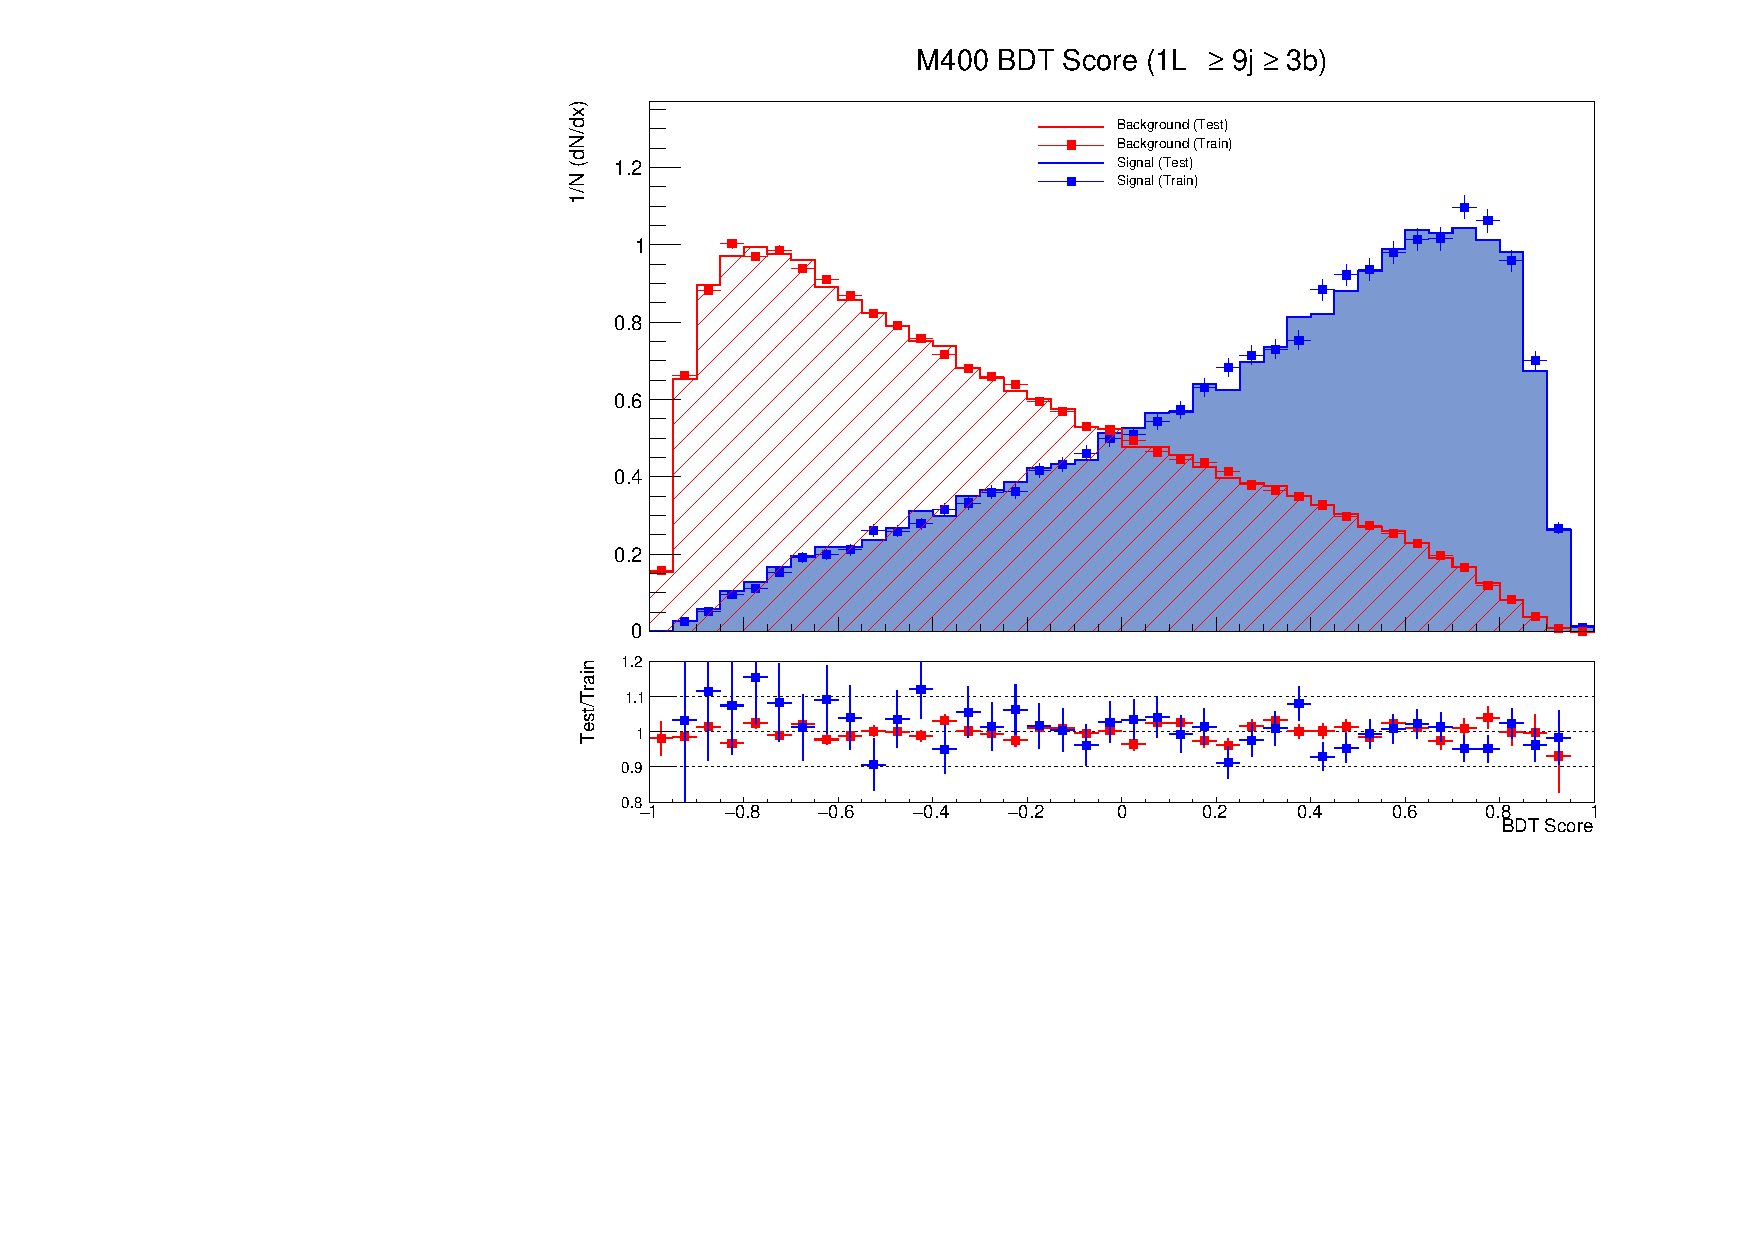
\includegraphics[width=\textwidth]{BDTScore/M400_BDT_1Lge9jge3b.pdf}
        \subcaption{M400 BDT}
    \end{subfigure}
   \begin{subfigure}[t]{0.49\textwidth}
        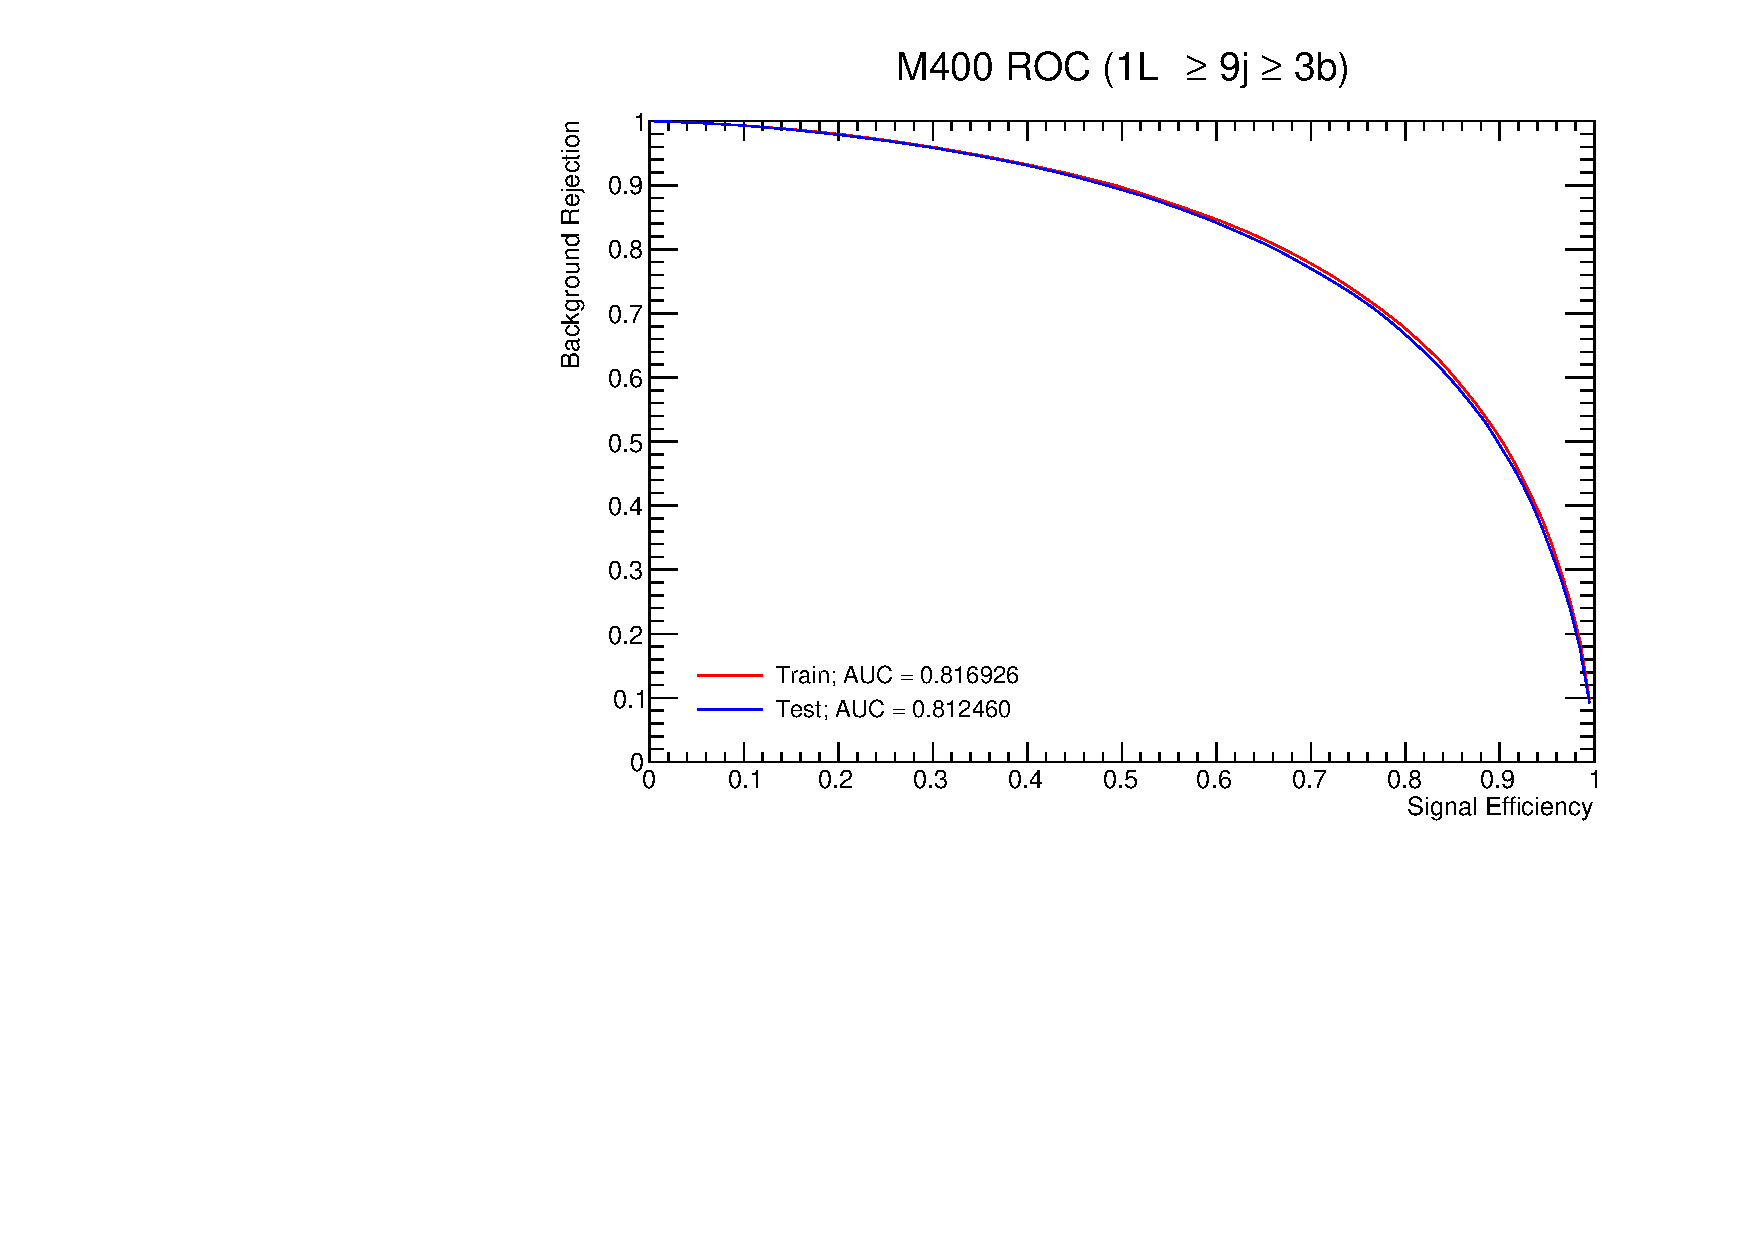
\includegraphics[width=\textwidth]{ROC/M400_ROC_1Lge9jge3b.pdf}
        \subcaption{M400 BDT - ROC}
    \end{subfigure}
    \begin{subfigure}[t]{0.49\textwidth}
        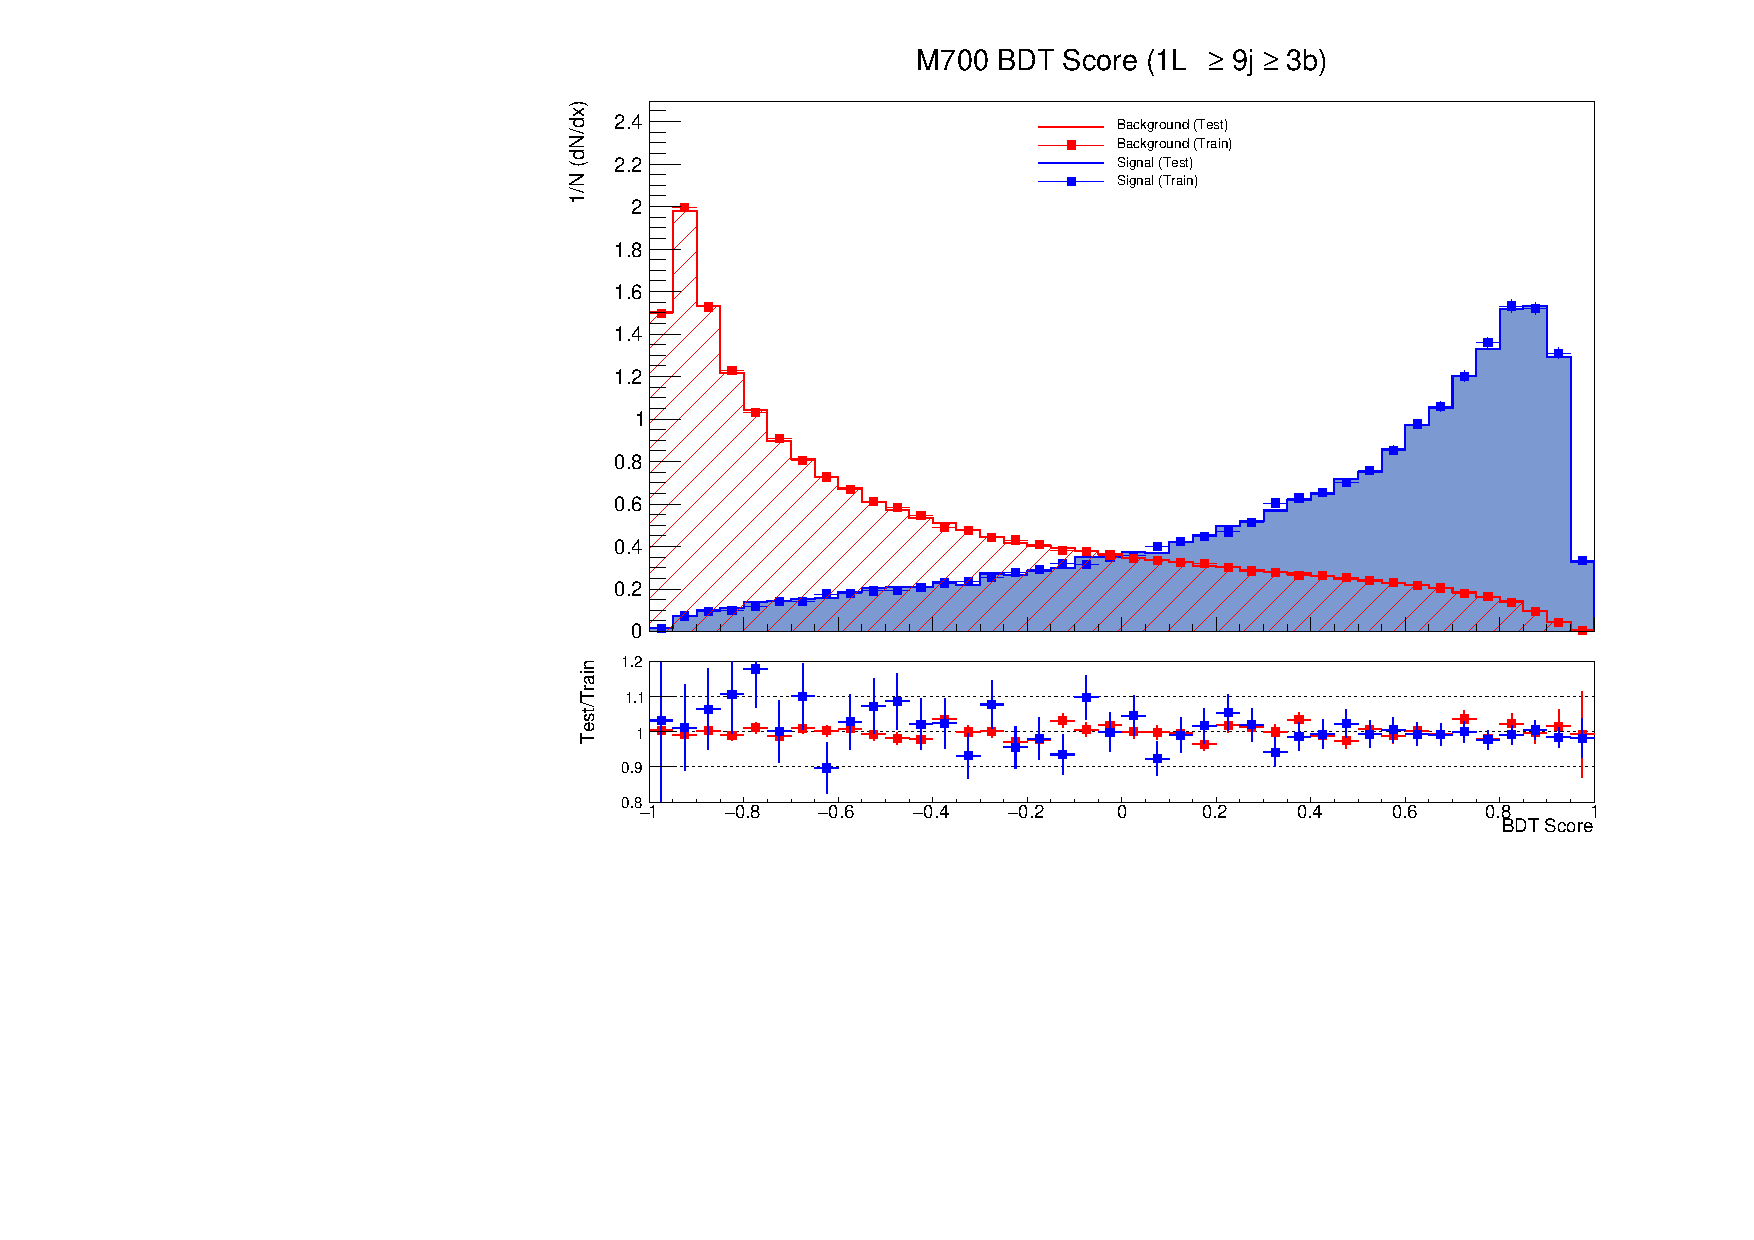
\includegraphics[width=\textwidth]{BDTScore/M700_BDT_1Lge9jge3b.pdf}
        \subcaption{M700 BDT}
    \end{subfigure}
     \begin{subfigure}[t]{0.49\textwidth}
        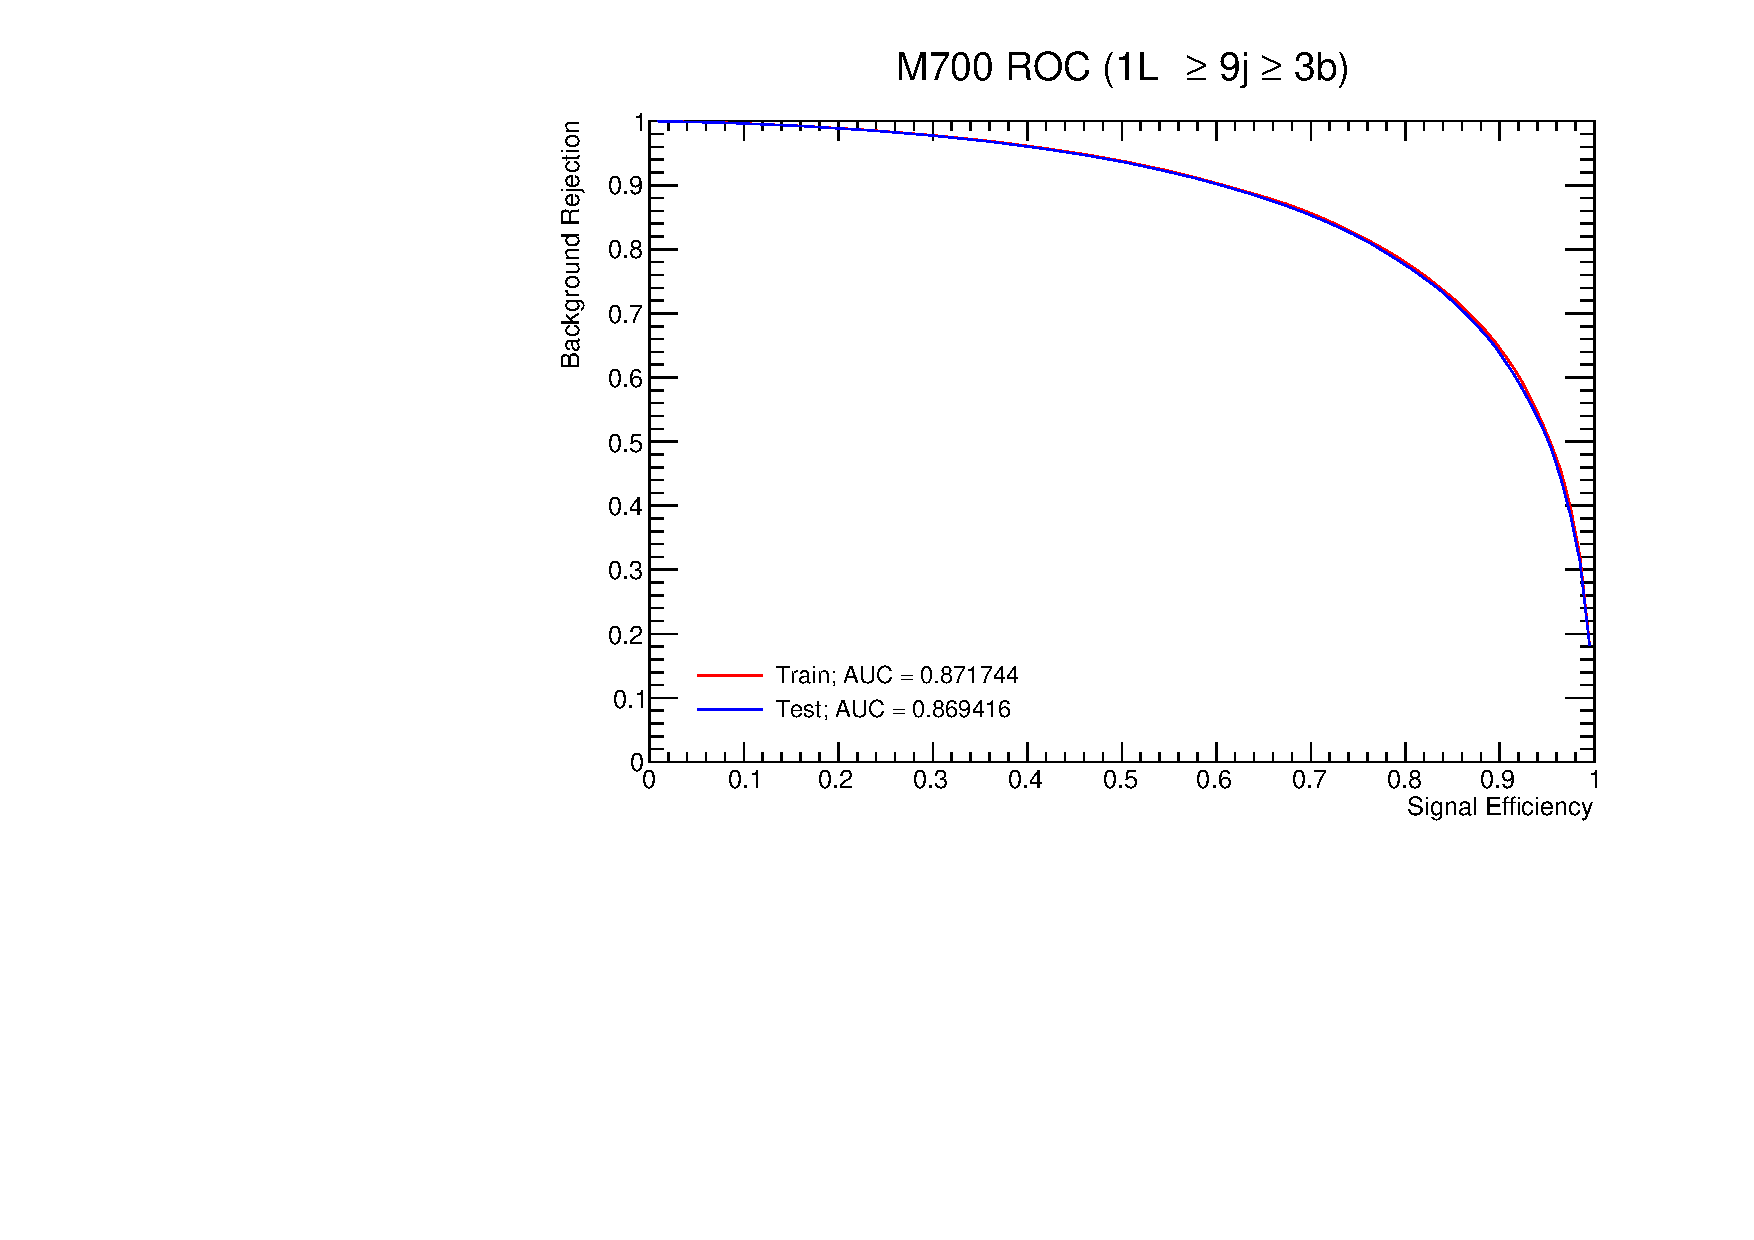
\includegraphics[width=\textwidth]{ROC/M700_ROC_1Lge9jge3b.pdf}
        \subcaption{M700 BDT}
    \end{subfigure}
    \begin{subfigure}[t]{0.49\textwidth}
        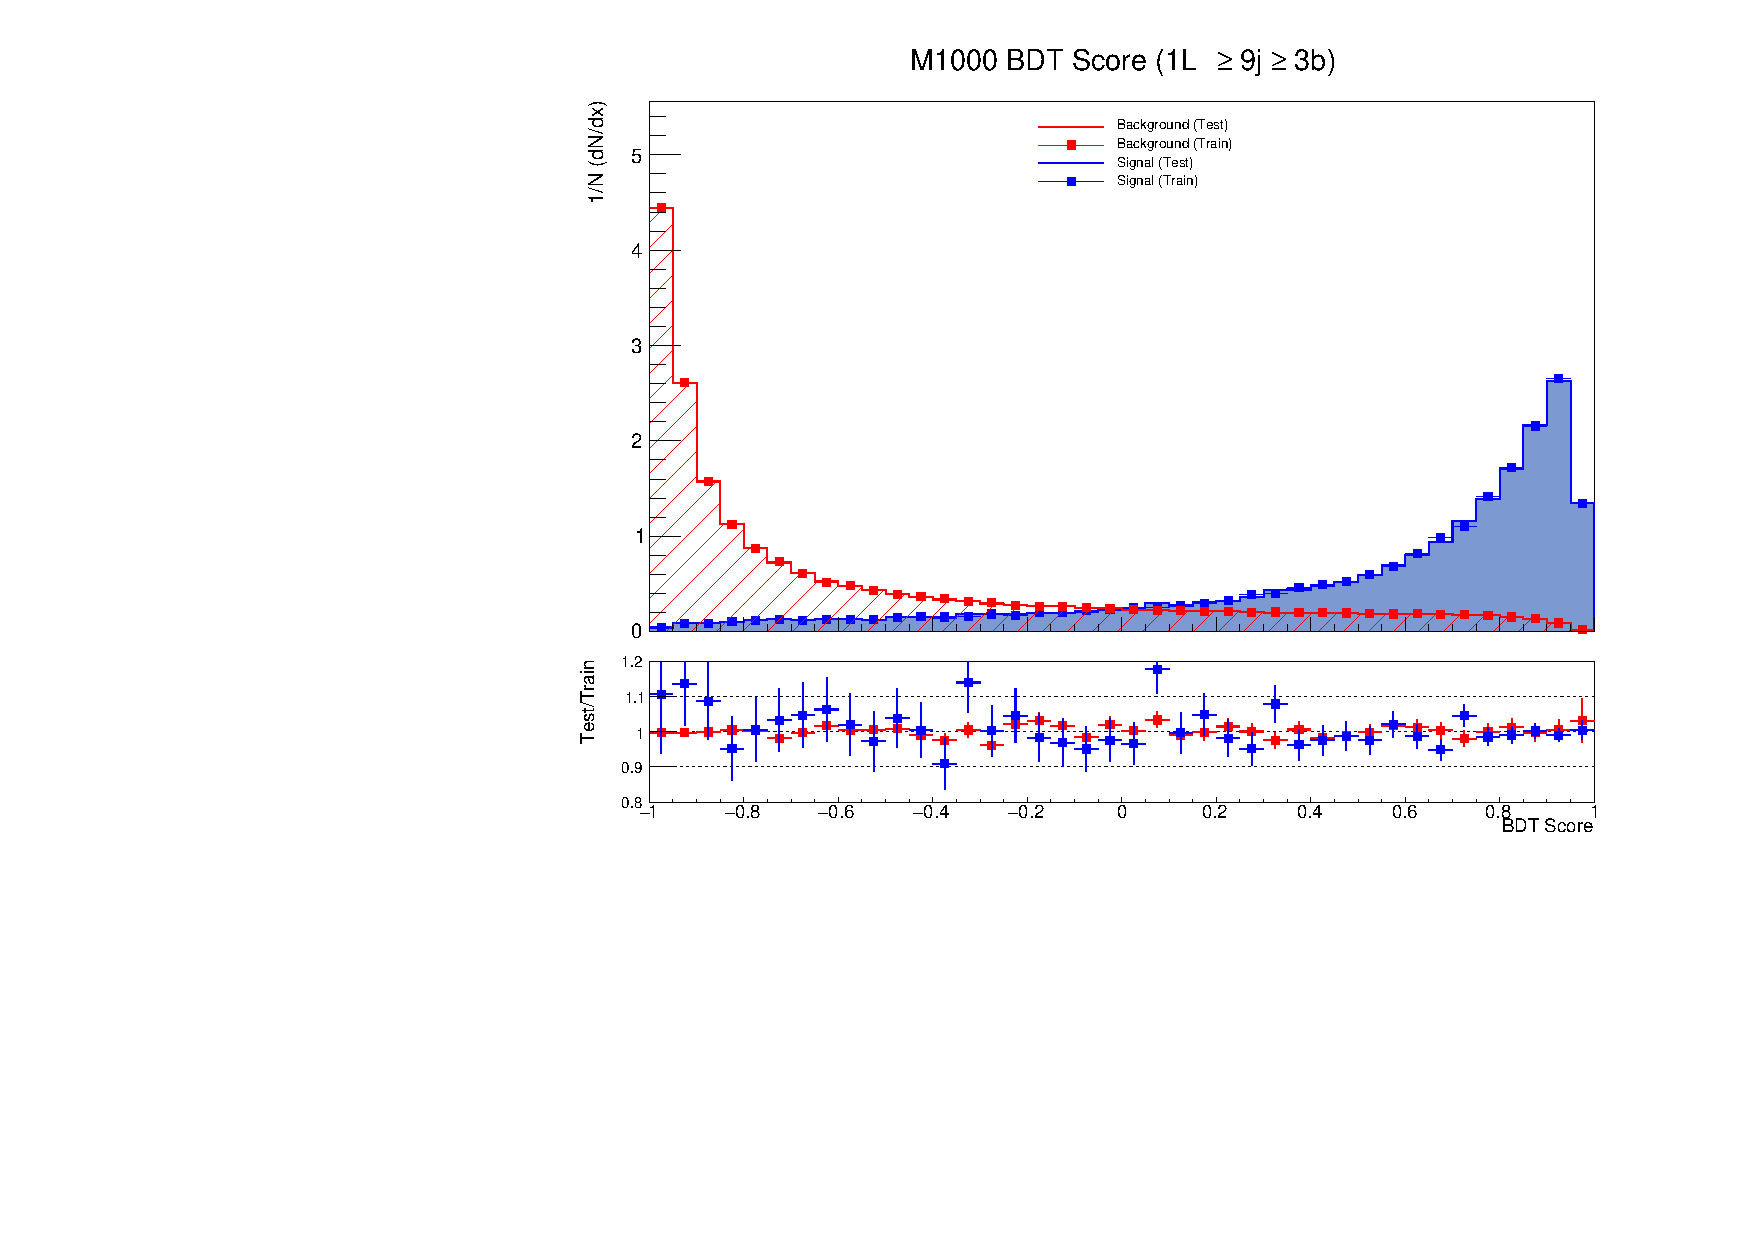
\includegraphics[width=\textwidth]{BDTScore/M1000_BDT_1Lge9jge3b.pdf}
        \subcaption{M1000 BDT}
     \end{subfigure}
     \begin{subfigure}[t]{0.49\textwidth}
        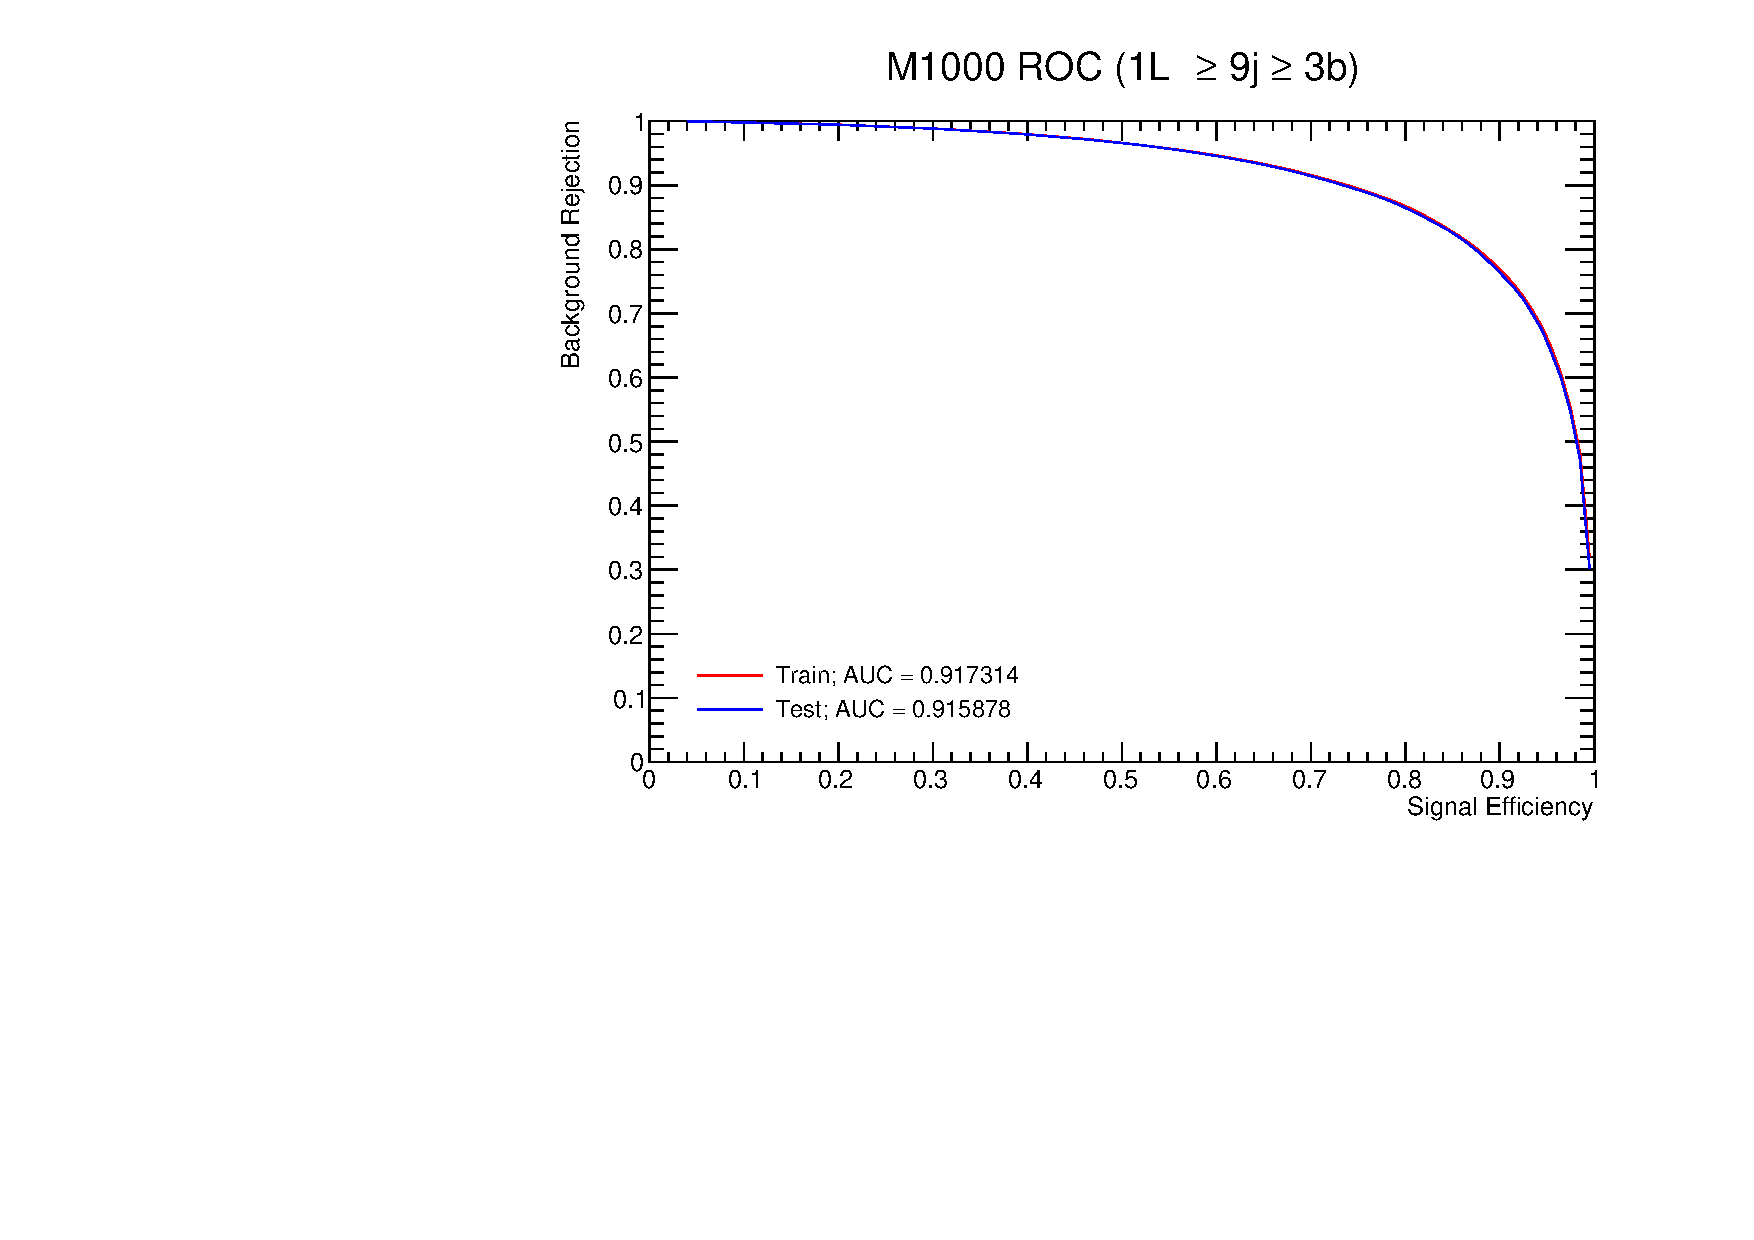
\includegraphics[width=\textwidth]{ROC/M1000_ROC_1Lge9jge3b.pdf}
        \subcaption{M1000 BDT}
    \end{subfigure}
\caption{\label{fig:1Lge9jge3bBDT} Figures in the left show both the training and testing BDT distribution between signal mass points at(a) $400~GeV$, (b) $700~GeV$ and (c) $1000~GeV$ and the $t\bar{t}+$jets background. Figures in the right show the ROC from both training and testing BDT. The region is in 1L$\geq 9j \geq 3b$.}
\end{figure}

\begin{figure}[!htp]\centering
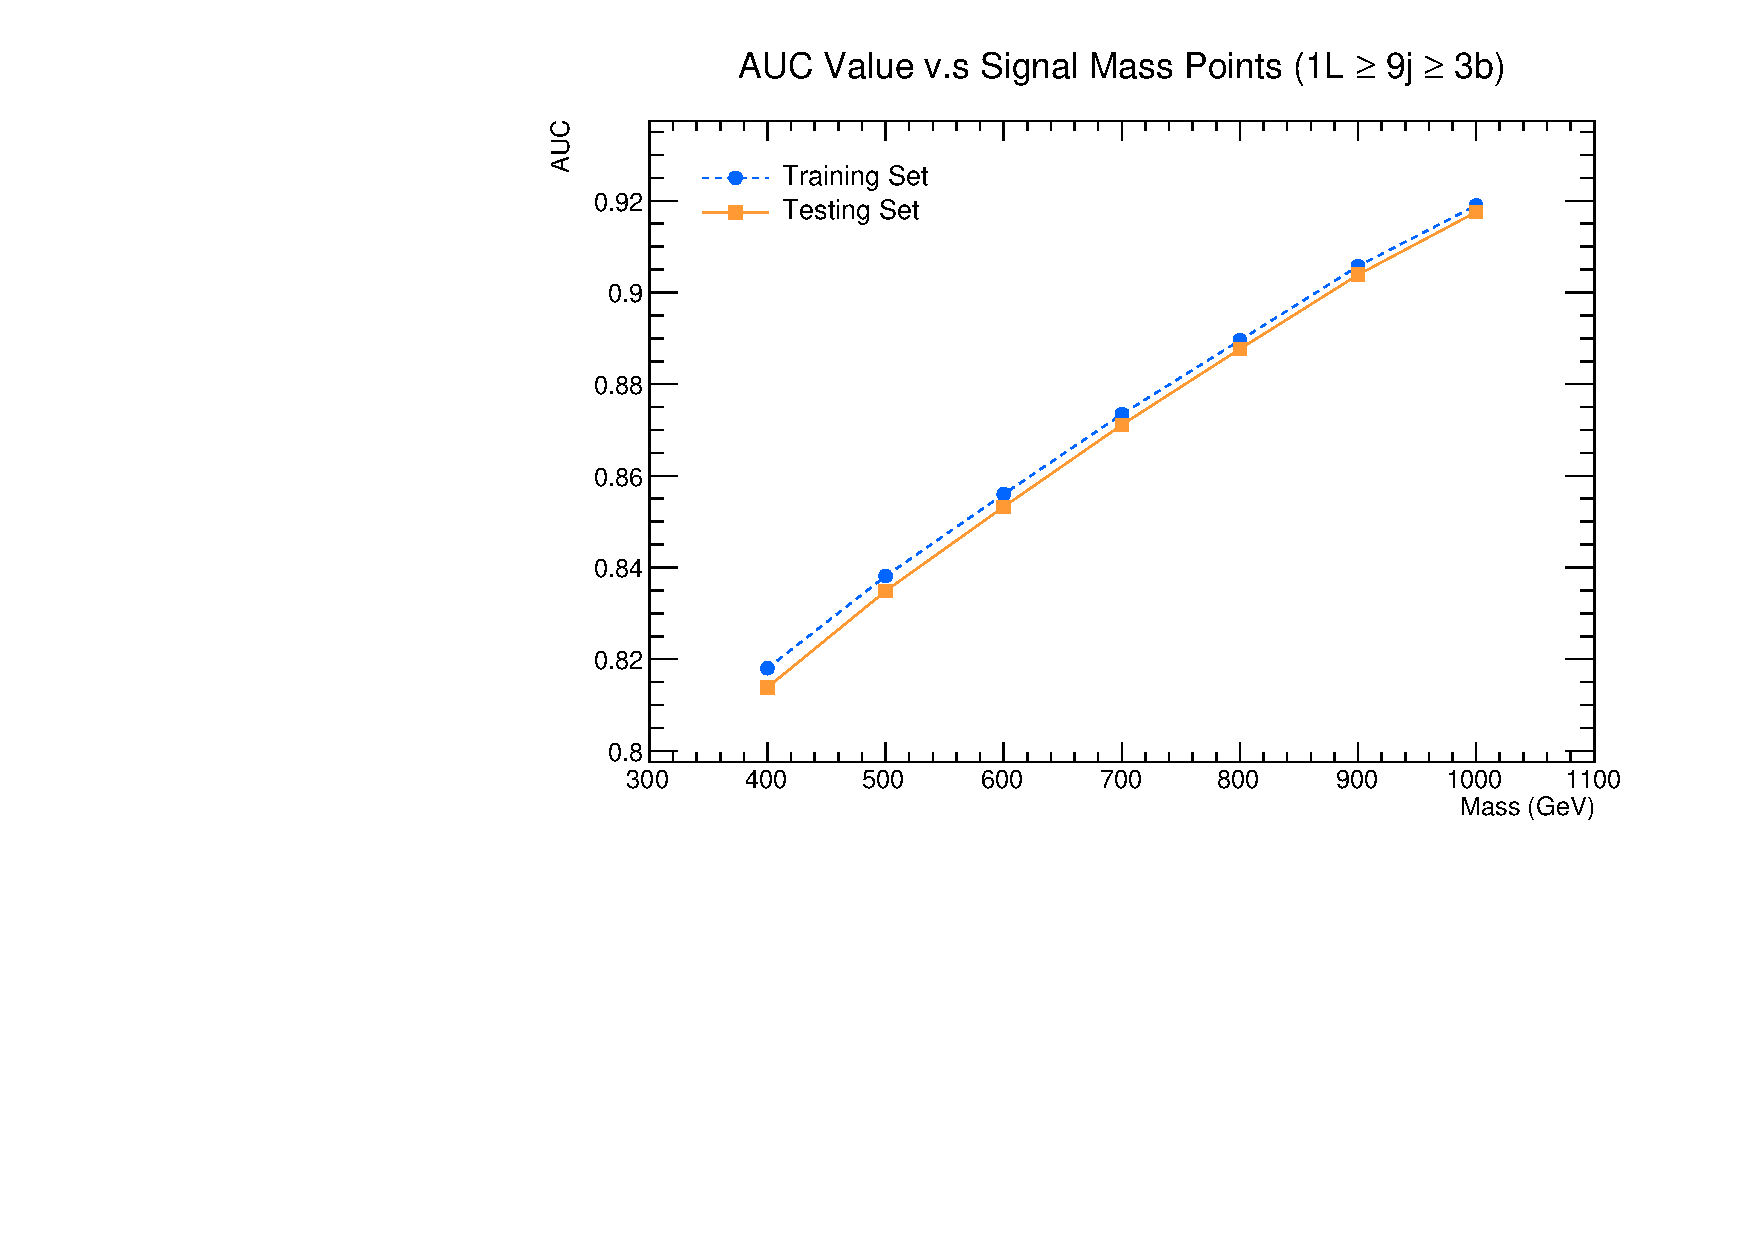
\includegraphics[width=0.45\textwidth]{AUC_perMP_1Lge9jge3b.pdf}
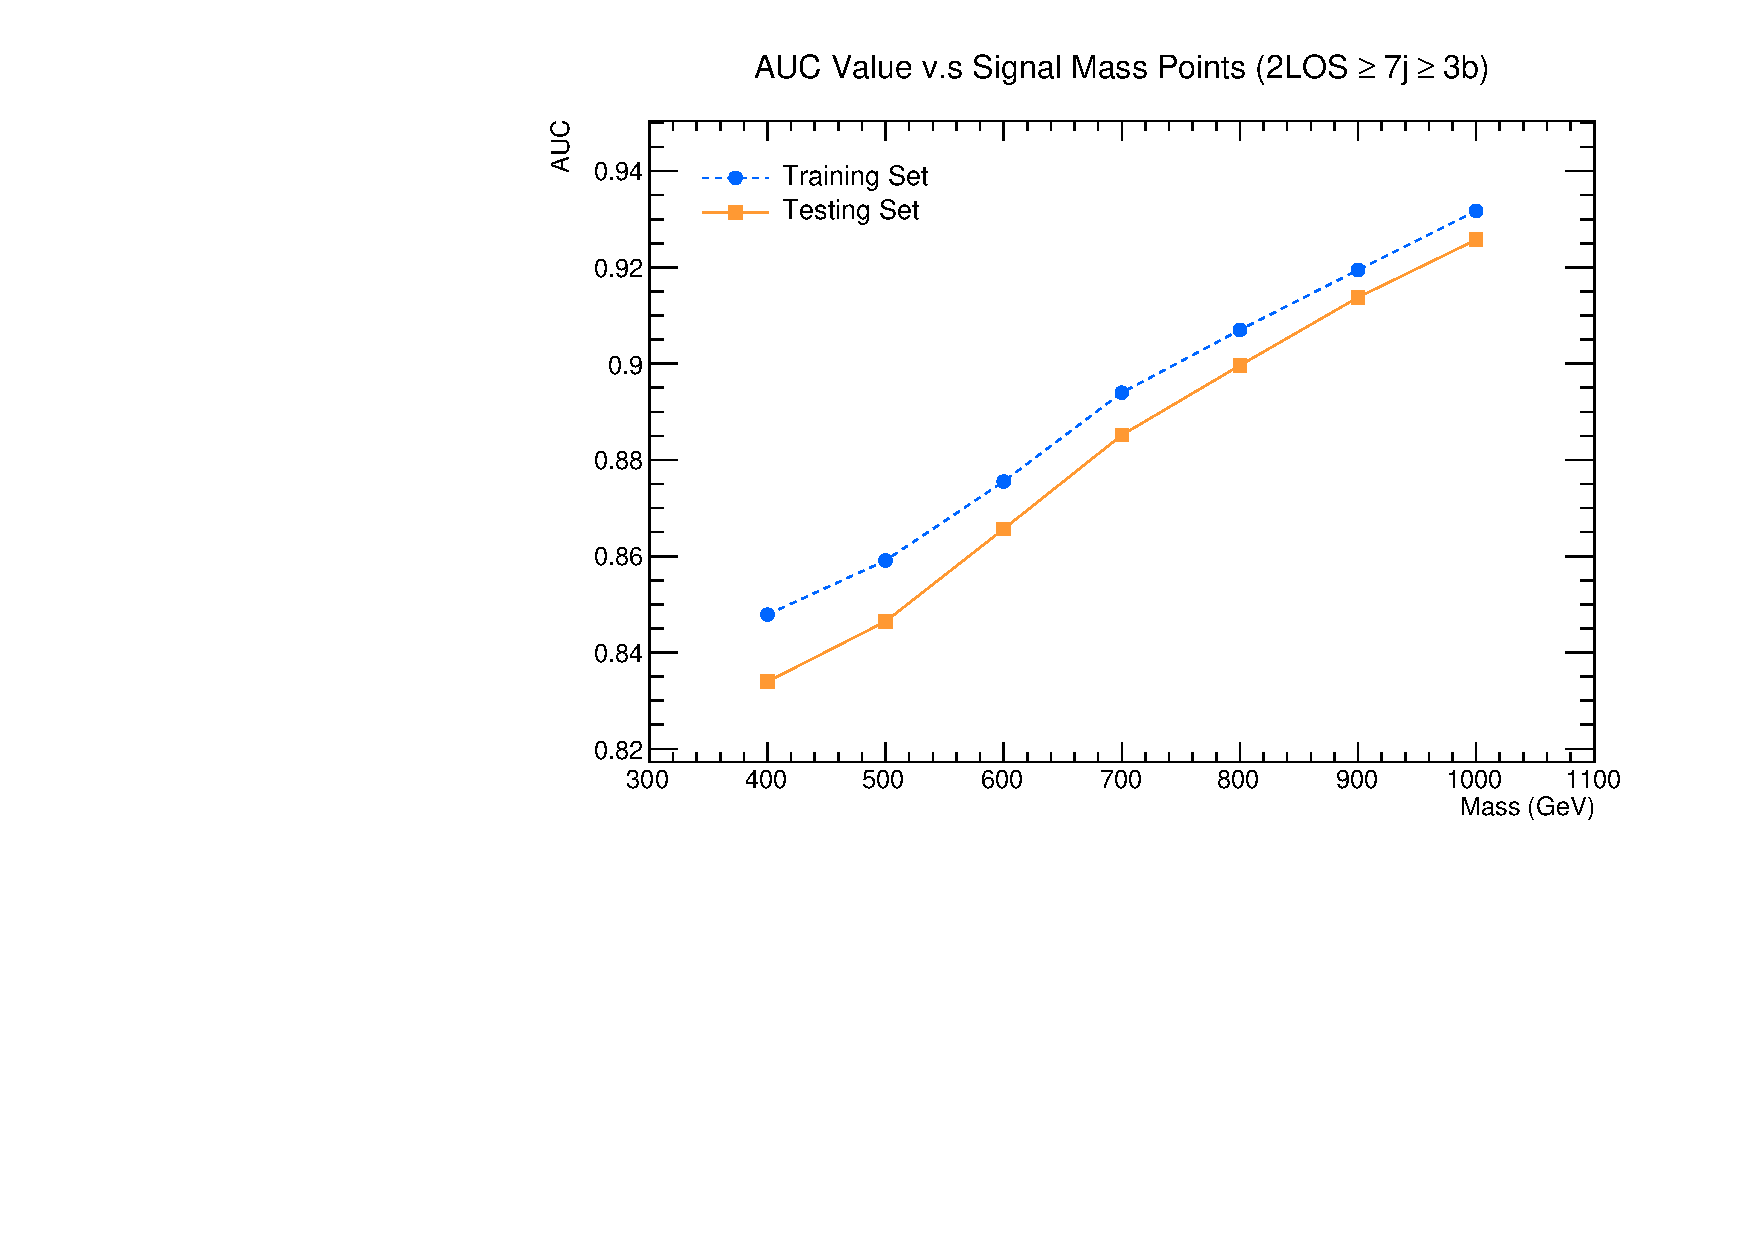
\includegraphics[width=0.45\textwidth]{AUC_perMP_2LOSge7jge3b.pdf}
\caption{\label{fig:AUC_perMP} Plots of AUC value from both training and testing samples against the studying signal mass points from $400~GeV$ to $1000~GeV$ in 1L$\geq 9j \geq 3b$ (left) and 2LOS$\geq 7j \geq 3b$(right).}
\end{figure}

\subsection{Graph Neural Network}% Callum
\label{sec:mva_gnn}
%

Graph neural networks (GNNs) are a class of ML models which operate on graph representations. Graphs are kind of data structure which describes a set objects (via nodes) and their relationships (via edges). GNNs capture the non-Euclidean arbitrary relational structure of graphs via so-called message-passing/graph-convolutional operations. As a consequence of message-passing operations, GNNs have inbuilt permutation invariance of nodes and edges. An additional useful feature of GNNs is that the same model can deal with graphs with any number of nodes or edges in stark contrast to FFNNs and BDTs which require a fixed input shape and ordering. In the context of event classifiers this allows low-level event objects and their relationships to be encoded on graphs with arbitrary object multiplicity. This analysis utilises a mass-parameterised GNN binary classifier to discriminate signal events against background events. A graph, $G$, which encodes an event and a pseudo mass, $m_H$, are input to the GNN as,

\begin{equation}
    y=\mathrm{GNN}(G, m_H)
\end{equation}

which returns a classification score, $y\in[0,1]$. The target classification scores are 0 for background and 1 for signal. 

\subsubsection{Graph Representation of Events and Input Variables}
In this section the construction of graphs from events will be detailed. The graphs constructed are homogeneous, fully-connected digraphs with no self connections. Within this framework an event graph is defined as a 3-tuple $G=(\textbf{u}, V, E)$ where:

\begin{itemize}
    \item $\textbf{u}$ is a vector of global features representing system level properties of the graph
    \item $V=\{\textbf{v}_i|i\in\{1,...,N\}\}$ is a set of $N$ nodes each carrying a vector, $\textbf{v}_i$, of node features corresponding to node $i$
    \item $E=\{\textbf{e}_{ij}|i\in\{1,...,N\},j\in\{1,...,N\}, i\neq j\}$ is a set of $N(N-1)$ directed edges each carrying a vector, $\textbf{e}_{ij}$, of edge features corresponding to the edge connecting node $i$ to node $j$ 
\end{itemize}
Events are represented on graphs by assigning reconstructed objects and corresponding object-level variables to graph nodes and encoding their respective geometric relationships on edges connecting them. Additionally, event-level variables are included via a set of global graph-level features. The node, edge and global features included on graphs are detailed below:
\begin{itemize}
\item \textbf{Nodes:} The reconstructed objects used to construct nodes include small-$R$ jets, muons, electrons and missing transverse energy. MET is included at node-level rather than as a global features so that the geometric relationship between $\phi_\mathrm{MET}$ and the other reconstructed objects can be encoded on edges. The node features are:
    \begin{itemize}
        \item[--] Object $p_\mathrm{T}$
        \item[--] Object $\eta$ (0 input for MET node)
        \item[--] Object $E$ 
        \item[--] Pseudo-continuous DL1r b-tagging score of the object (0 for non-jets)
        \item[--] Object type encoding number (-2 for muons, -1 for electrons, 0 for MET and 1 for jets)
    \end{itemize}
Object $\phi$ as a node feature is excluded since the $\phi$ geometry of the event is fully captured through the relative $\Delta\phi$ information encoded on directed edges between objects. Removal of absolute $\phi$ values enforces a global $\phi$ symmetry to the graph. A separate scaling factor is applied to each node feature. Fixed scaling factors, $s$, are chosen to map features $x$->$x$/$s$ such that the maximal value of the scaled feature is approximately 1.

\item \textbf{Edges:} Graphs are constructed as fully-connected digraphs by creating an edge for every possible permutation of node pairs. Edge features are calculated from object coordinates in the $(\phi,\eta)$-plane. The edge features are:
    \begin{itemize}
        \item[--] $\Delta \phi$ between pairs of objects
        \item[--] $\Delta \eta$ between pairs of objects
        \item[--] $\Delta R$ between pairs of objects
    \end{itemize}
Separate scaling factors are applied to $\Delta\phi$ and $\Delta\eta$. $\Delta R$ is scaled by the sum of these scaling factors. Fixed scaling factors, $s$, are chosen to map features $x$->$x$/$s$ such that the maximal value of the scaled feature is approximately 1.


\item \textbf{Globals:} The event-level features included in the global variable set include simple bulk properties of the event such as $N_\mathrm{jets}$ and $H_T$ but also high-level reconstructed variables which have been shown to provide discriminating power. The set of variables is adapted from the BDT input set detailed in section \ref{sec:BDT-input-variables} by removing features otherwise included via nodes e.g leading jet $p_\mathrm{T}$ and MET. The global features are:
    \begin{itemize}
        \item[--] $H_T=\sum_i \pT^i$ where the sum is over all reconstructed jets and leptons
        \item[--] The $H_T$ of the first 4 leading jets ranked in order of descending \pt divided by the $H_T$ of the remaining jets, $\sum_{i<4}\pt^i/\sum_{i\geq4}\pt^i$
        \item[--] Average invariant mass of jets triplets with separation $\Delta R<3$
        \item[--] For the 2L channel only: Invariant mass of the dilepton pair  $m_{ll}$
        \item[--] For the 1L channel only: $W^\pm$ reconstructed transverse mass $m_T(l,E_\mathrm{T}^\mathrm{miss})$
        \item[--] Jet multiplicity $N_\mathrm{jets}$
        \item[--] Number of RC-jets with mass greater than 100 GeV
        \item[--] Average invariant mass of b-tagged jet triplets
        \item[--] Minimum $\Delta R$ among pairs of b-tagged jet and lepton
        \item[--] Minimum $\Delta R$ among pairs of b-tagged jets
        \item[--] Centrality $\sum_i \pt^i/\sum_i E_i$ where the sums are performed over all reconstructed jets and leptons
        \item[--] Average $\Delta R$ across all jet pairs
        \item[--] Sum of pseudo-continuous b-tagging scores, $\sum_{i<6}pcb_i$, of the first 6 jets ranked in order of descending DL1r scores
        \item[--] Sum of the first $k_t$ splitting scale $d_{12}$ over all RC-jets
        \item[--] Sum of the second $k_t$ splitting scale $d_{23}$ over all RC-jets
    \end{itemize}

\end{itemize}


\subsubsection{A Parameterised General Message Passing GNN}

In this section the inner workings of the message-passing layers developed and the construction of the GNN used in this analysis will be discussed. The GNN used in this analysis is built using the \texttt{PyTorch Geometric} package. In particlular, the \texttt{MetaLayer(torch.nn.Module)} class is utilised which provides a generic building block for creating general GNNs inspired by the framework established in \cite{https://doi.org/10.48550/arxiv.1806.01261}. Within this framework a GNN layer can be split into three models: an edge updating model, a node updating model and a global updating model. Upon application the \texttt{MetaLayer} updates the input graph by applying the edge update followed by the node update followed by the global update. The edge, node and global models are classes which can be explicitly programmed using \texttt{PyTorch}. In this section the forward pass mechanisms of each model will be defined.

\begin{itemize}
    \item \textbf{Edge updating model:} An edge connecting nodes $i$ to node $j$ is updated via
    \begin{equation}
        \textbf{e}_{ij}'=f_\mathrm{edge}(\textbf{v}_i,\textbf{v}_j,\textbf{e}_{ij}, \textbf{u})
    \end{equation}
    where $f_\mathrm{edge}$ is a trainable neural network which takes as inputs the node feature vectors, $\textbf{v}_i$ and $\textbf{v}_j$, of the two nodes, the edge feature vector, $\textbf{e}_{ij}$, of the edge connecting them and the global feature vector $\textbf{u}$ and outputs a vector $\textbf{e}_{ij}'$ which is used as the updated edge feature vector. This is repeated for all edges in the graph yielding an updated edge set $E'$.
    
    \item \textbf{Node updating model:} Message-passing takes place in the node updating model. A message, $\textbf{m}_{ij}$, is constructed for each edge connecting node $i$ to node $j$ via
    \begin{equation}
        \textbf{m}_{ij}=f_\mathrm{message}(\textbf{v}_i,\textbf{v}_j,\textbf{e}_{ij}')
    \end{equation}
    where $f_\mathrm{message}$ is a trainable neural network which takes as inputs the feature vectors of nodes $i$ and $j$ and the updated edge feature vector connecting them. An aggregation function, $A$, is used to construct an aggregated message, $\textbf{M}_i$, for node $i$ as
    \begin{equation}
        \textbf{M}_{i}=A(\{\textbf{m}_{ij}|j\in\{1,...,N\},j\neq i\})
    \end{equation}
    from the set of $N-1$ neighbouring messages. The node feature vector is then updated via
    \begin{equation}
        \textbf{v}_{i}'=f_\mathrm{node}(\textbf{v}_i,\textbf{M}_i,\textbf{u})
    \end{equation}
    where $f_\mathrm{node}$ is a trainable neural network which takes as inputs the feature vector of node $i$, the corresponding aggregated message vector and the global feature vector and outputs the updated node feature vector $\textbf{v}_{i}'$. This is repeated for all nodes in the graph yielding an updated node set $V'$.
    
    \item \textbf{Global updating model:} An aggregated vector of node features  for the graph is created via
    The global feature vector is updated via 
    \begin{equation}
        \textbf{u}'=f_\mathrm{global}(\textbf{u}, A(V'))
    \end{equation}
    where $f_\mathrm{global}$ is a trainable neural network and the aggregation function, $A$, acts on the set of updated node features, $V'$. 
\end{itemize}

The resulting output after the edge, node and global models are applied is an updated graph, $G'=(\textbf{u}',V',E')$. The dimensionality of the node, edge and global feature vectors in the updated graph may increase or decrease with respect to the input graph. Generally graph updating layers may be applied successively $n$ times resulting in a final output graph $G^{(n)}=(\textbf{u}^{(n)},V^{(n)},E^{(n)})$. For graph classification problems the final output graph must be converted to an output vector which in binary classification is simply an single output score. The output classification score, y, is obtained via

\begin{equation}
    y=f_\mathrm{out}(\textbf{u}^{(n)}, A(V^{(n)}))
\end{equation}
 
 where $f_\mathrm{out}$ is a trainable neural network and the aggregation function, $A$, aggregates the node features in the final output graph. 

\label{subsubsec:how-gnn-works}



\subsubsection{Architecture and Hyperparameter Setup}

In this section the architecture of each GNN model used in the analysis will be detailed as well as the hyperparameter and learning settings. It will be useful in this section to define a notation  $N_\mathrm{feats}(G)=(N^\mathrm{global}_\mathrm{feats},N^\mathrm{node}_\mathrm{feats},N^\mathrm{edge}_\mathrm{feats})$ to describe the number of global, node and edge features in a graph, $G$. 

Both the 1L and 2LOS GNN models apply a sequence of $n$ graph updating layers and a final fully connected layer as described in section \ref{subsubsec:how-gnn-works}. For simplicity many parameters are kept the same for both GNN models and for all layers within models:
\begin{itemize}
    \item All trainable NNs within the models contain a single hidden layer with 32 nodes and ReLU activation functions
    \item All message-passing layers utilise a message vector with 12 features
    \item All graph updating layers yield output graphs with $N_\mathrm{feats}(G')=(9,12,6)$
    \item A sigmoid activation function is applied to the output of the final fully connected layer
    \item All aggregation functions return a vector of the maximum and mean of each feature from the set of input feature vectors
\end{itemize}

Differences between the models are motivated by the lower statistics in the 2LOS channel. The model complexity is decreased and the droput is increased in the 2LOS GNN to reduce overtraining:
\begin{itemize}
    \item \textbf{1L GNN:}
    \begin{itemize}
    \item Graph updating layers: $n=3$
    \item Dropout: $p=0.10$
    \end{itemize}
    \item \textbf{2LOS GNN:}
    \begin{itemize}
    \item Graph updating layers: $n=2$
    \item Dropout: $p=0.25$
    \end{itemize}
\end{itemize}

The same learning parameters are used to train both models, they are:

\begin{itemize}
    \item Optimiser: Adam with parameters: 
    \begin{itemize}
        \item Learning rate, $\gamma=0.001$
        \item $\beta_1=0.9$
        \item $\beta_2=0.999$
        \item $\epsilon=10^{-8}$
        \item $\lambda=0$
    \end{itemize}
    \item Loss function: Binary cross entropy
\end{itemize}
The loss is calculated for each event and weighted by the absolute event weight. The loss per batch is then calculated as the average over the per event losses in a batch.

\subsubsection{GNN Performance}

In this section the results from the trained 1L and 2LOS GNN models will be shown and their performance evaluated. Each model is cross-trained using a 2-fold splitting of the data set. The splitting is performed by taking either even or odd event numbers.
During the training, sample weights are calculated such that background/signal is balanced across all pseudo-mass/mass points, i.e.$\sum w(Bkg,m) = \sum w(Sig,m)$ and $\sum w(Sig,400~GeV)=\sum w(Sig,500~GeV)=...=\sum w(Sig,1000~GeV)$.
This is achieved by reweighting each signal sample by a factor of $1/\sum events(Sig,m)$ and each background sample by a factor of $7/\sum events(Bkg)$, where 7 is the number of mass points since pseudo-mass is sampled uniformly.
The output score of the cross-trained model is evaluated by using the model trained on even events to evaluate odd events and vice-versa. The area under ROC curve (AUC) is used as a performance metric and the difference between training and testing AUC is used as a metric of overtraining. A selection of score distributions is shown in figures \ref{fig:1l-gnn-scores} and \ref{fig:2los-gnn-scores} which show that training and testing distributions are consistent for both odd and even trained models. AUC against mass point is shown for both models in figure \ref{fig:AUCvsMass-1LOS}. An increase in over-training is seen in the 2LOS model and fluctuations are visible when plotting in regions with low statistics, this is expected due to the statistics available in 2LOS. The level of over-training is below $1\%$ in the 1L channel and $\sim2\%$ in the 2LOS channel which is acceptable.

The figure \ref{fig:gnn-AUC-mass} shows the AUC for various combinations of pseudomass inputs used to get the GNN weight for all background and signal samples and signal samples. The best performance is achieved when using the pseudomass corresponding to the mass in the simulated signal sample, as expected (the diagonal). When extracting limits, we perform a separate profile likelihood fit for each signal mass point - always the same pseudomass is used for background and signal samples as is the target signal mass point. Pseudo-masses are assigned randomly to background events by sampling possible values with equal probability. This approach functions in the same way that selecting a separately trained MVA for each mass point would. However, incorporating it as an input variable effectively allows weight sharing between each mass point training and increases the number of signal statistics in the training.

\begin{figure}[t!]
    \centering
    \begin{subfigure}[t]{\textwidth}
        \centering
        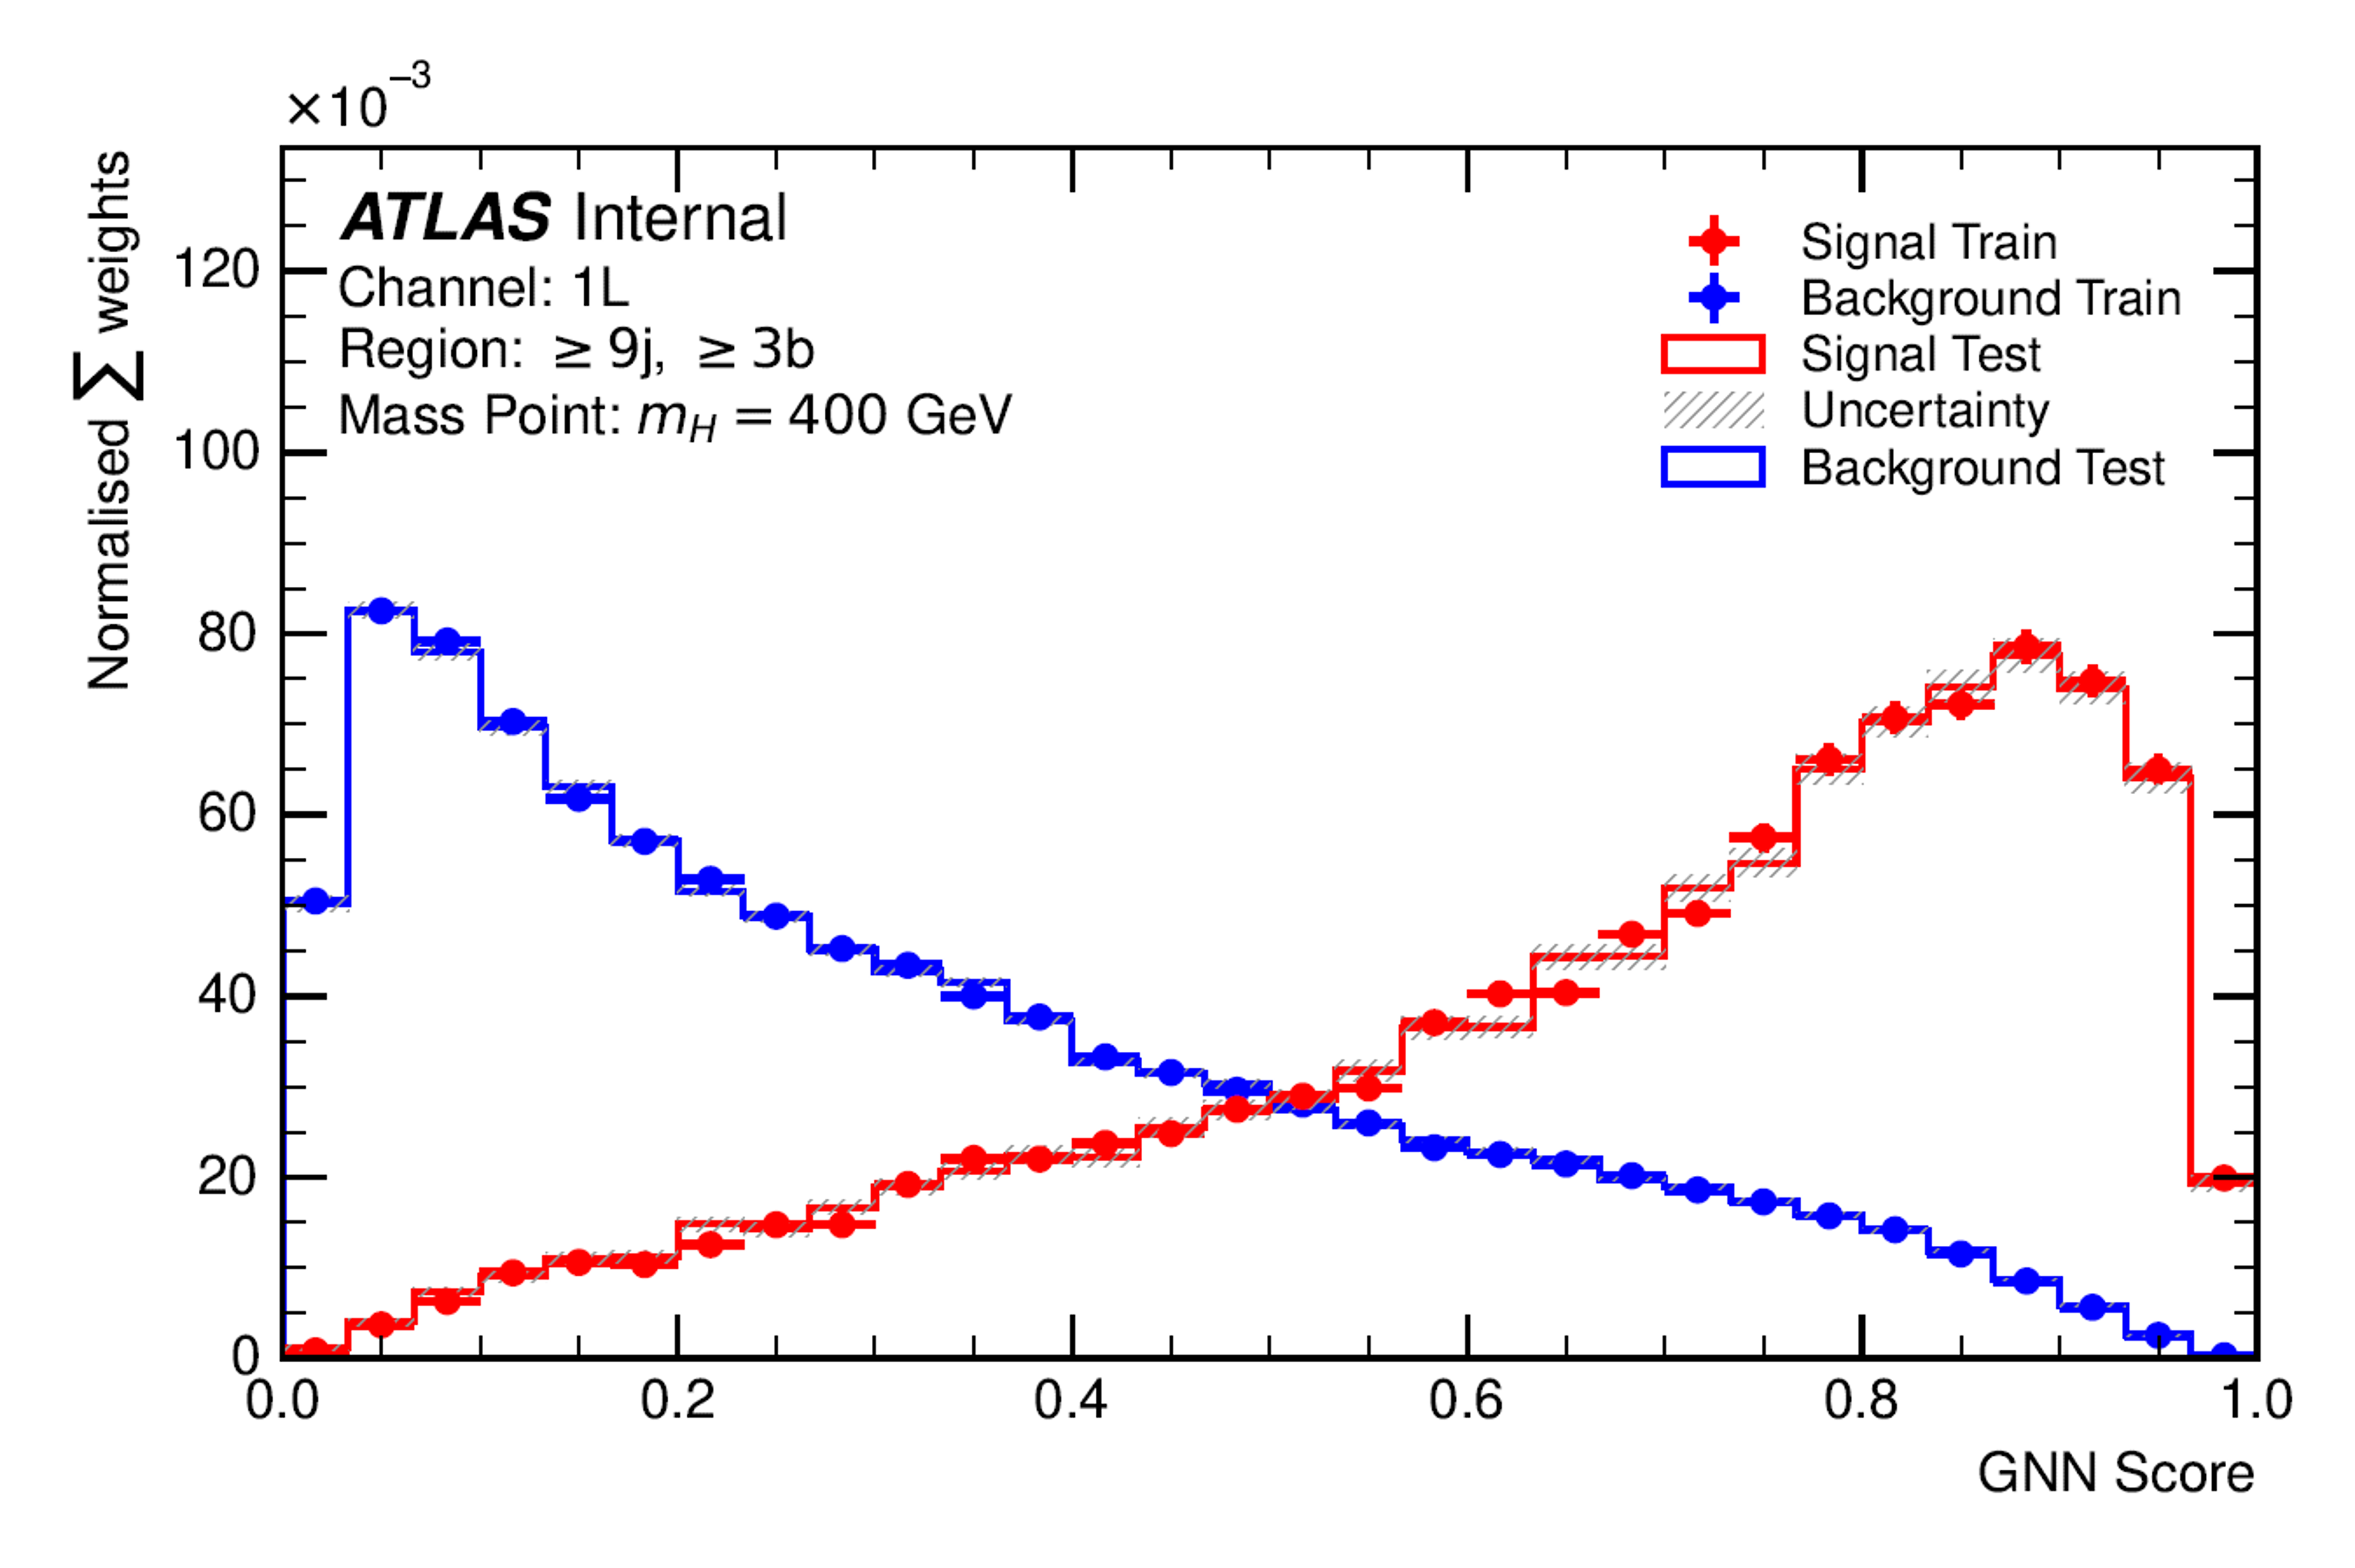
\includegraphics[width=0.48\textwidth]{figures/gnn/Plots_1L/400/GNN_Score_Plot_400GeV_Inclusive.png}
        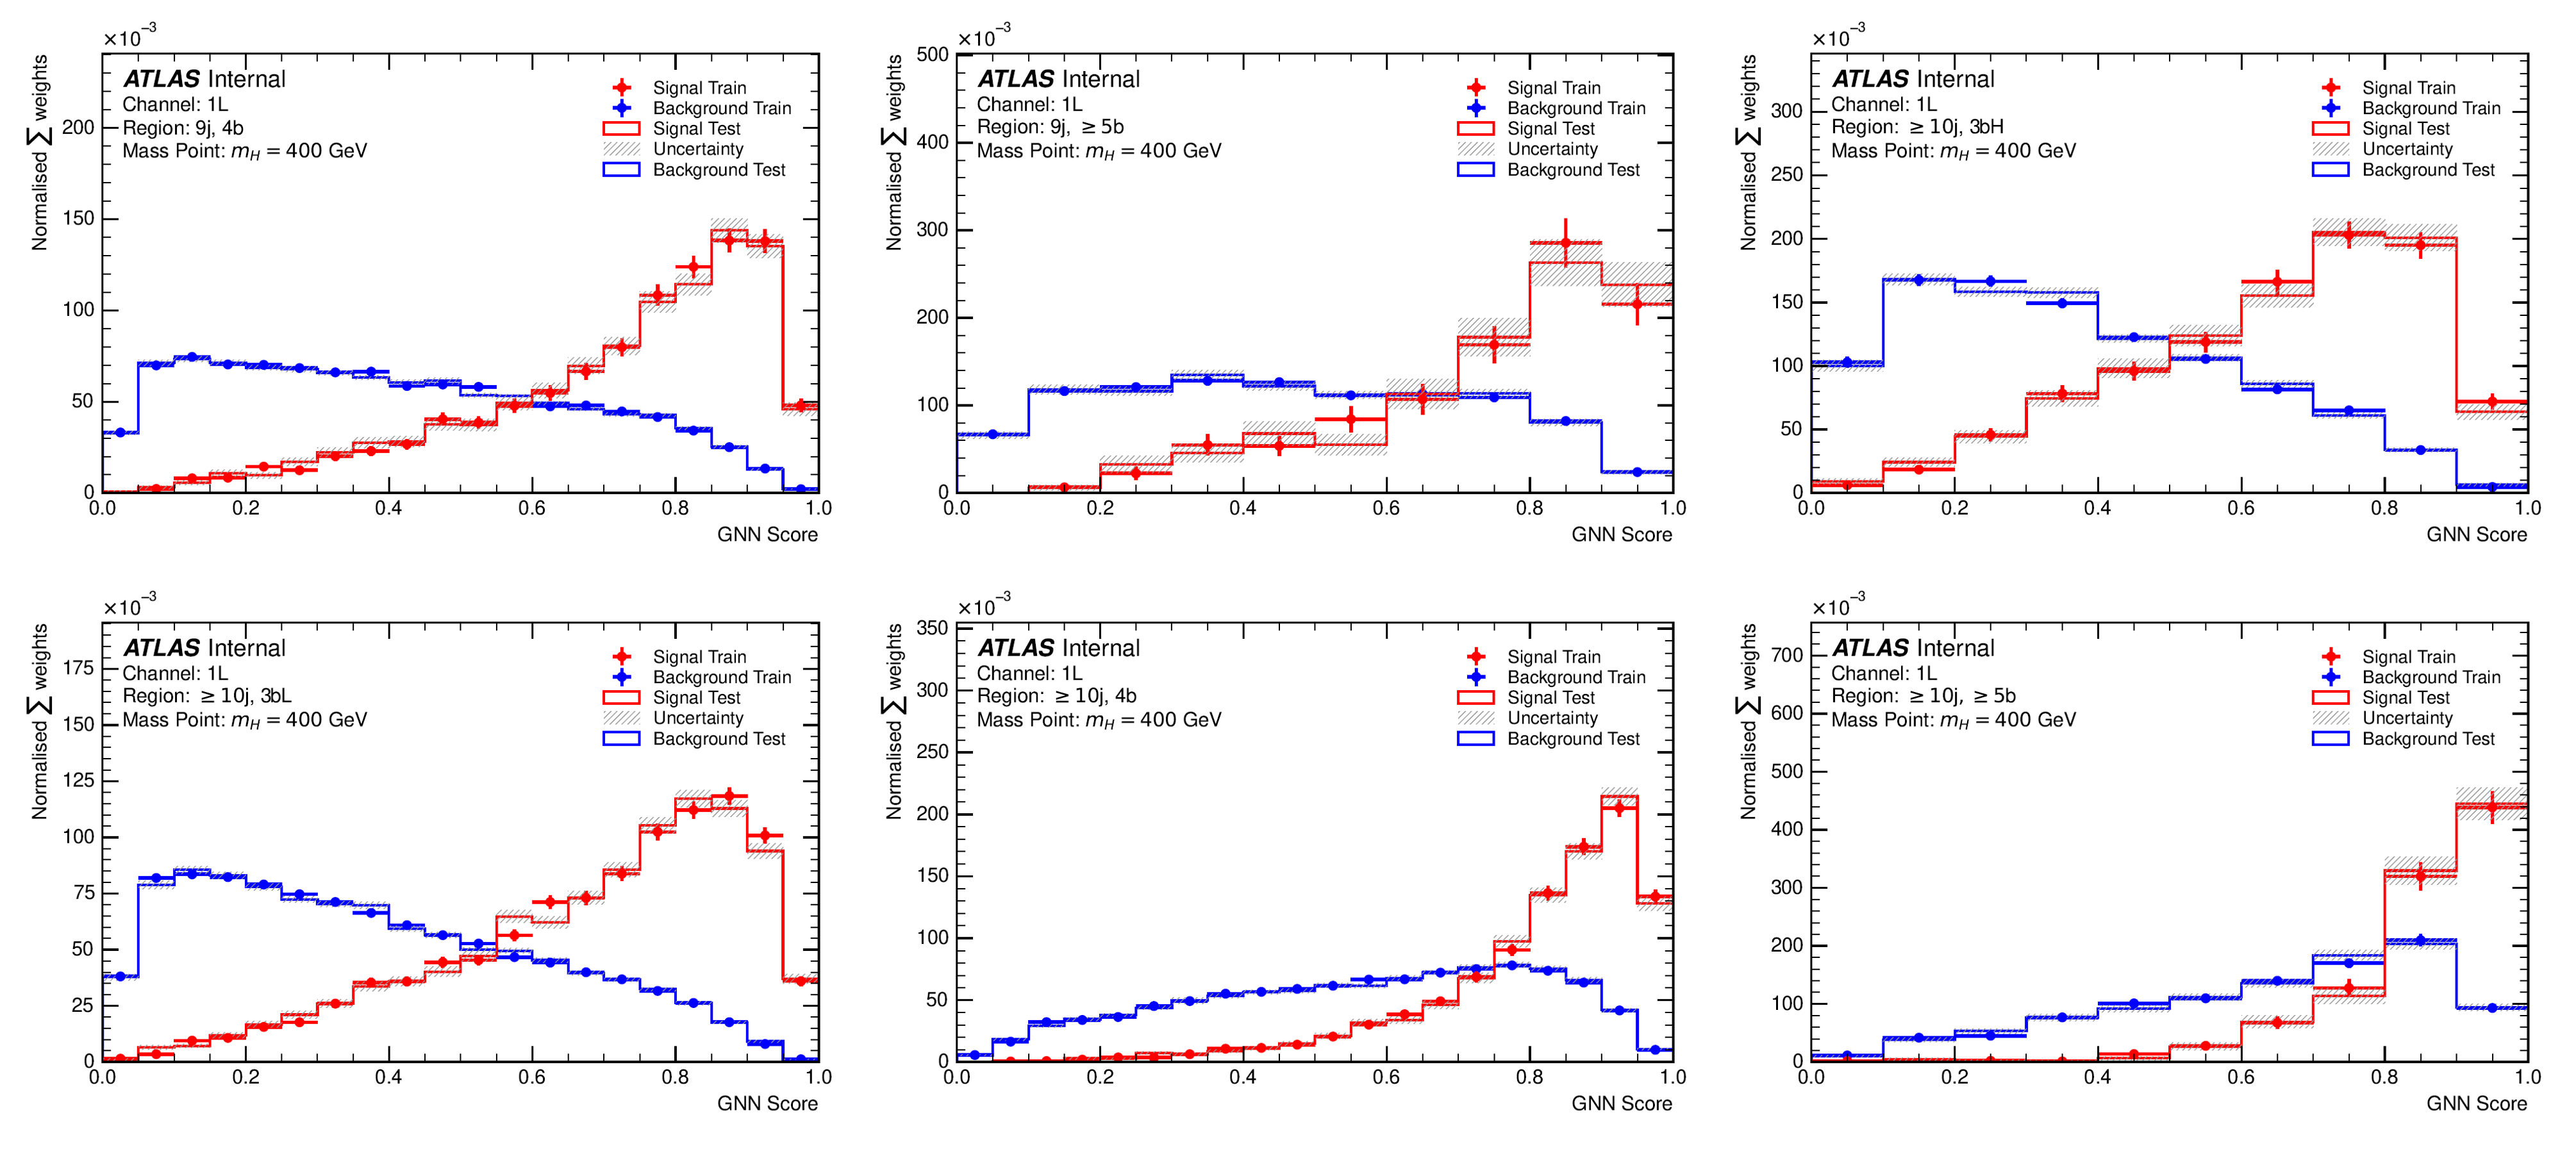
\includegraphics[width=0.48\textwidth]{figures/gnn/Plots_1L/400/GNN_Score_Plot_400GeV_Split.png}
        \caption{400 GeV mass point}
    \end{subfigure}
    \bigskip
    \centering
    \begin{subfigure}[t]{\textwidth}
        \centering
        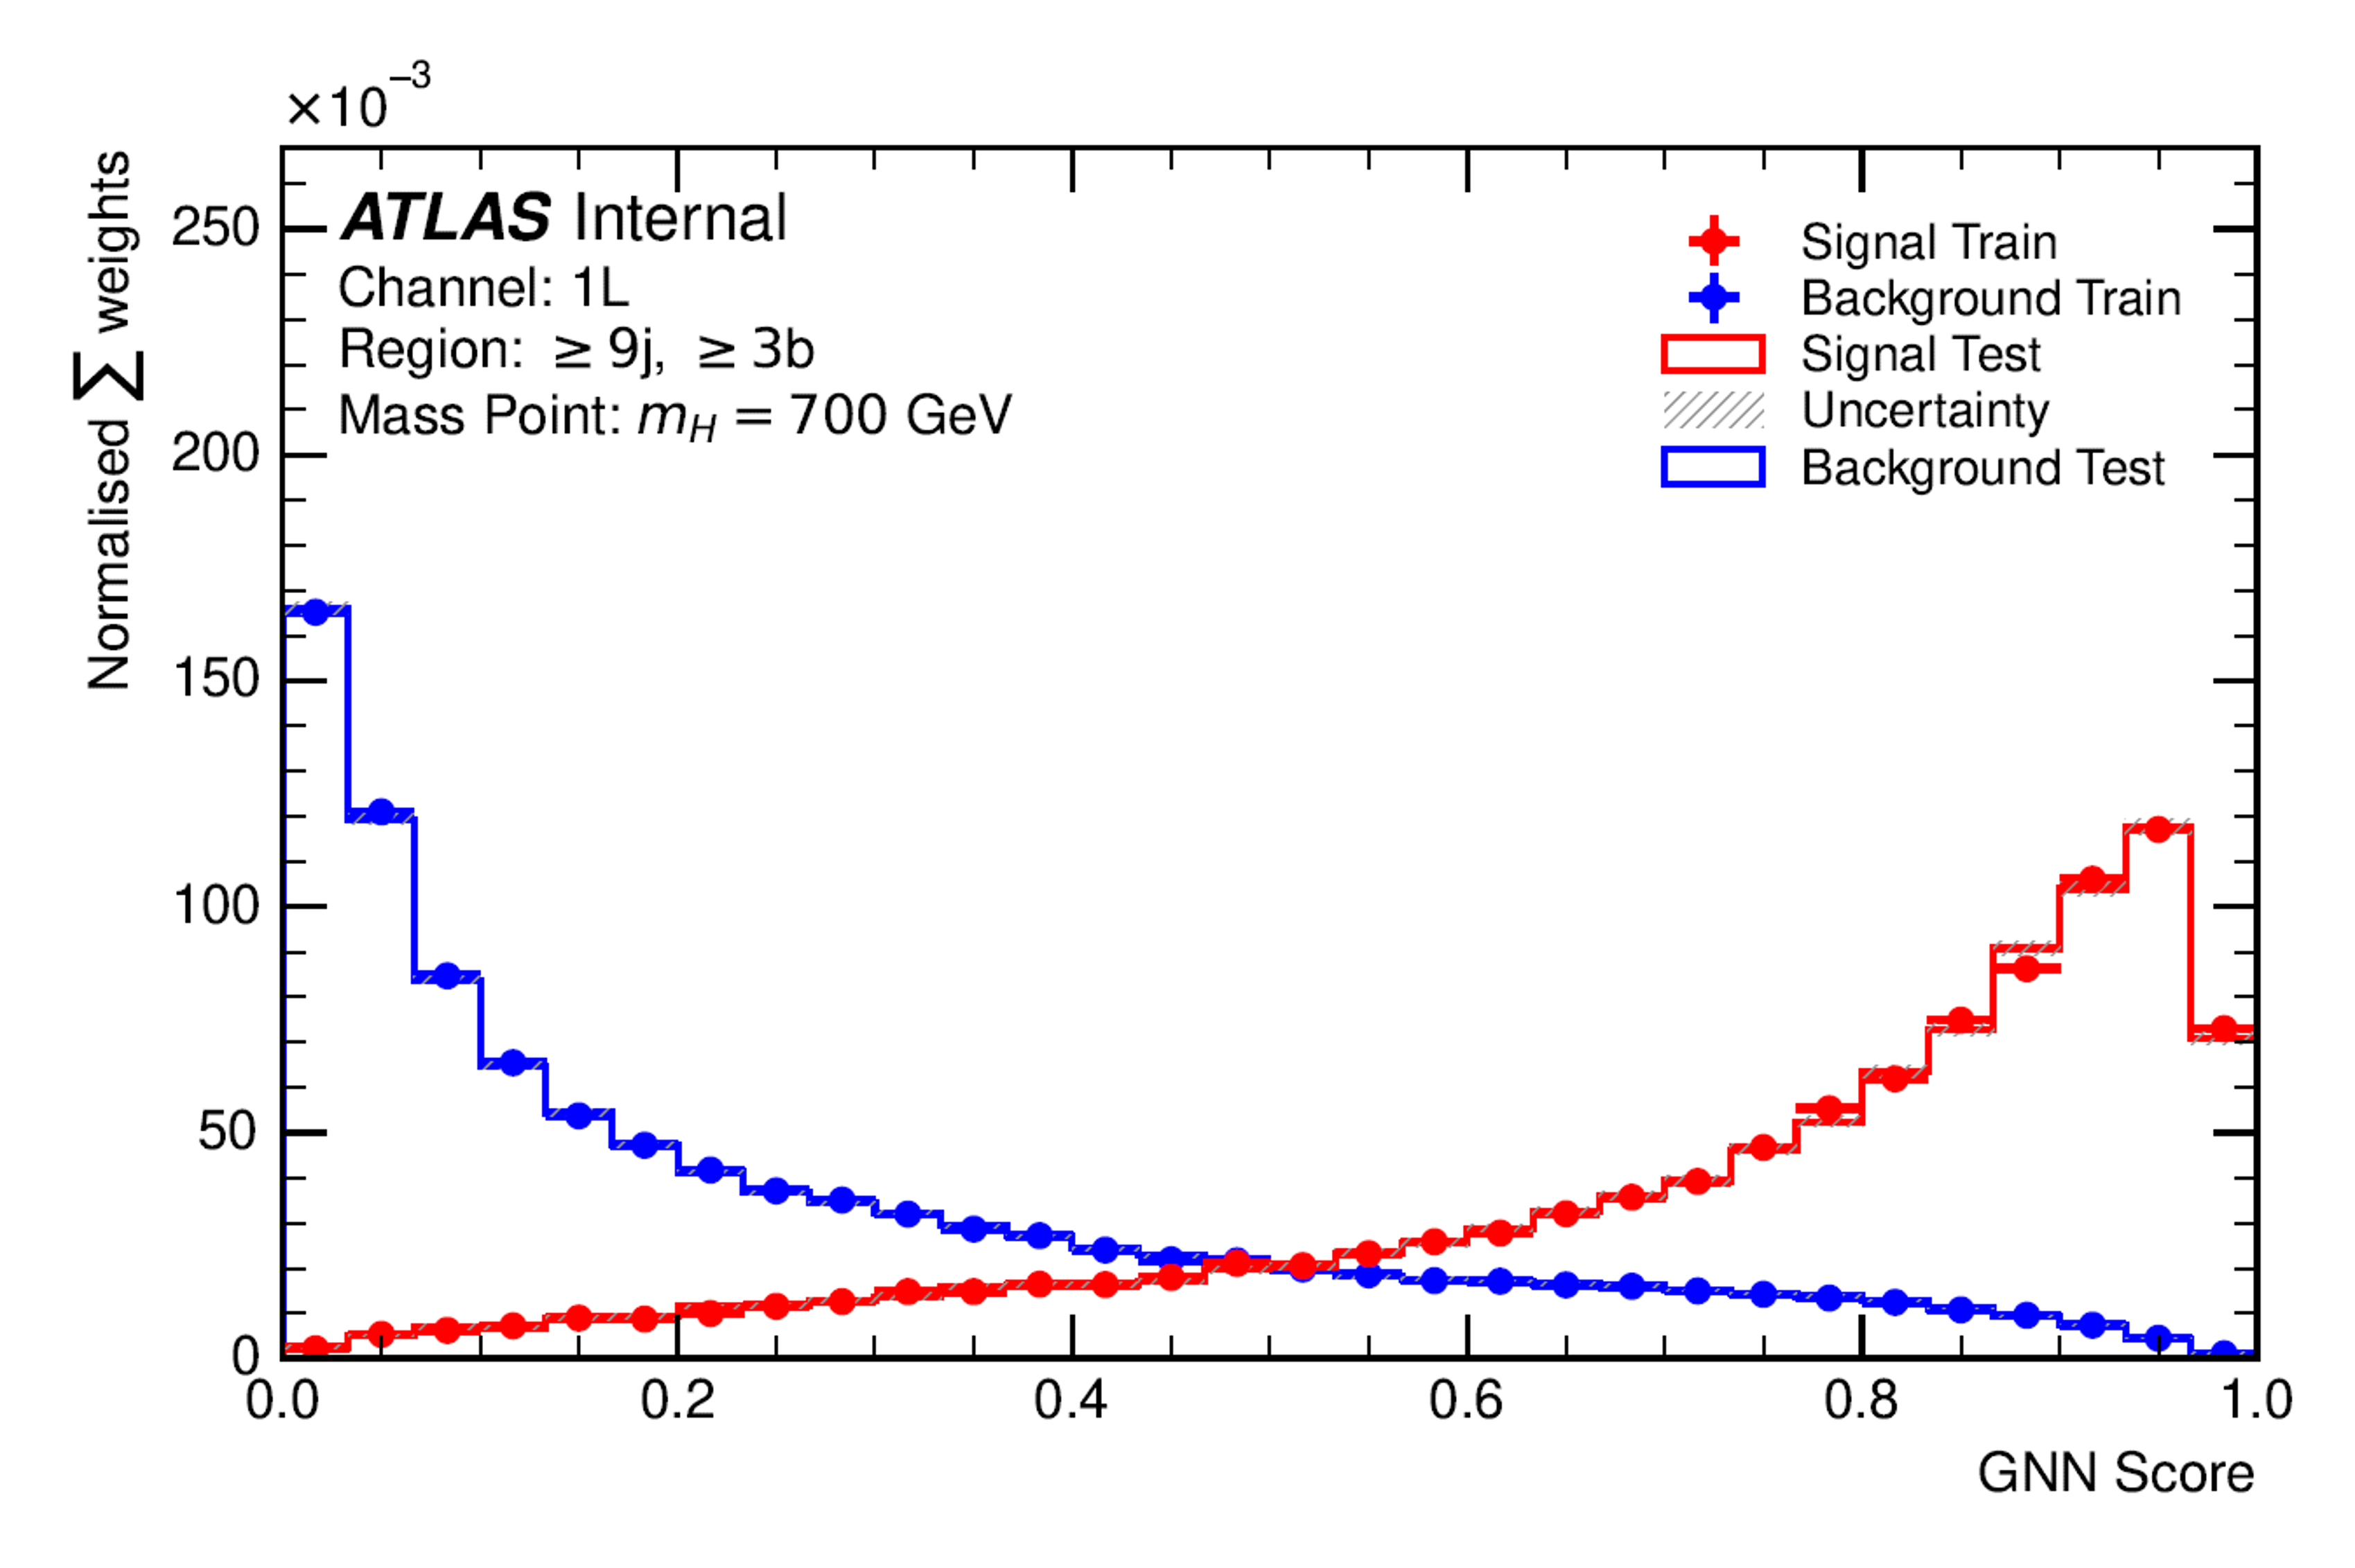
\includegraphics[width=0.48\textwidth]{figures/gnn/Plots_1L/700/GNN_Score_Plot_700GeV_Inclusive.png}
        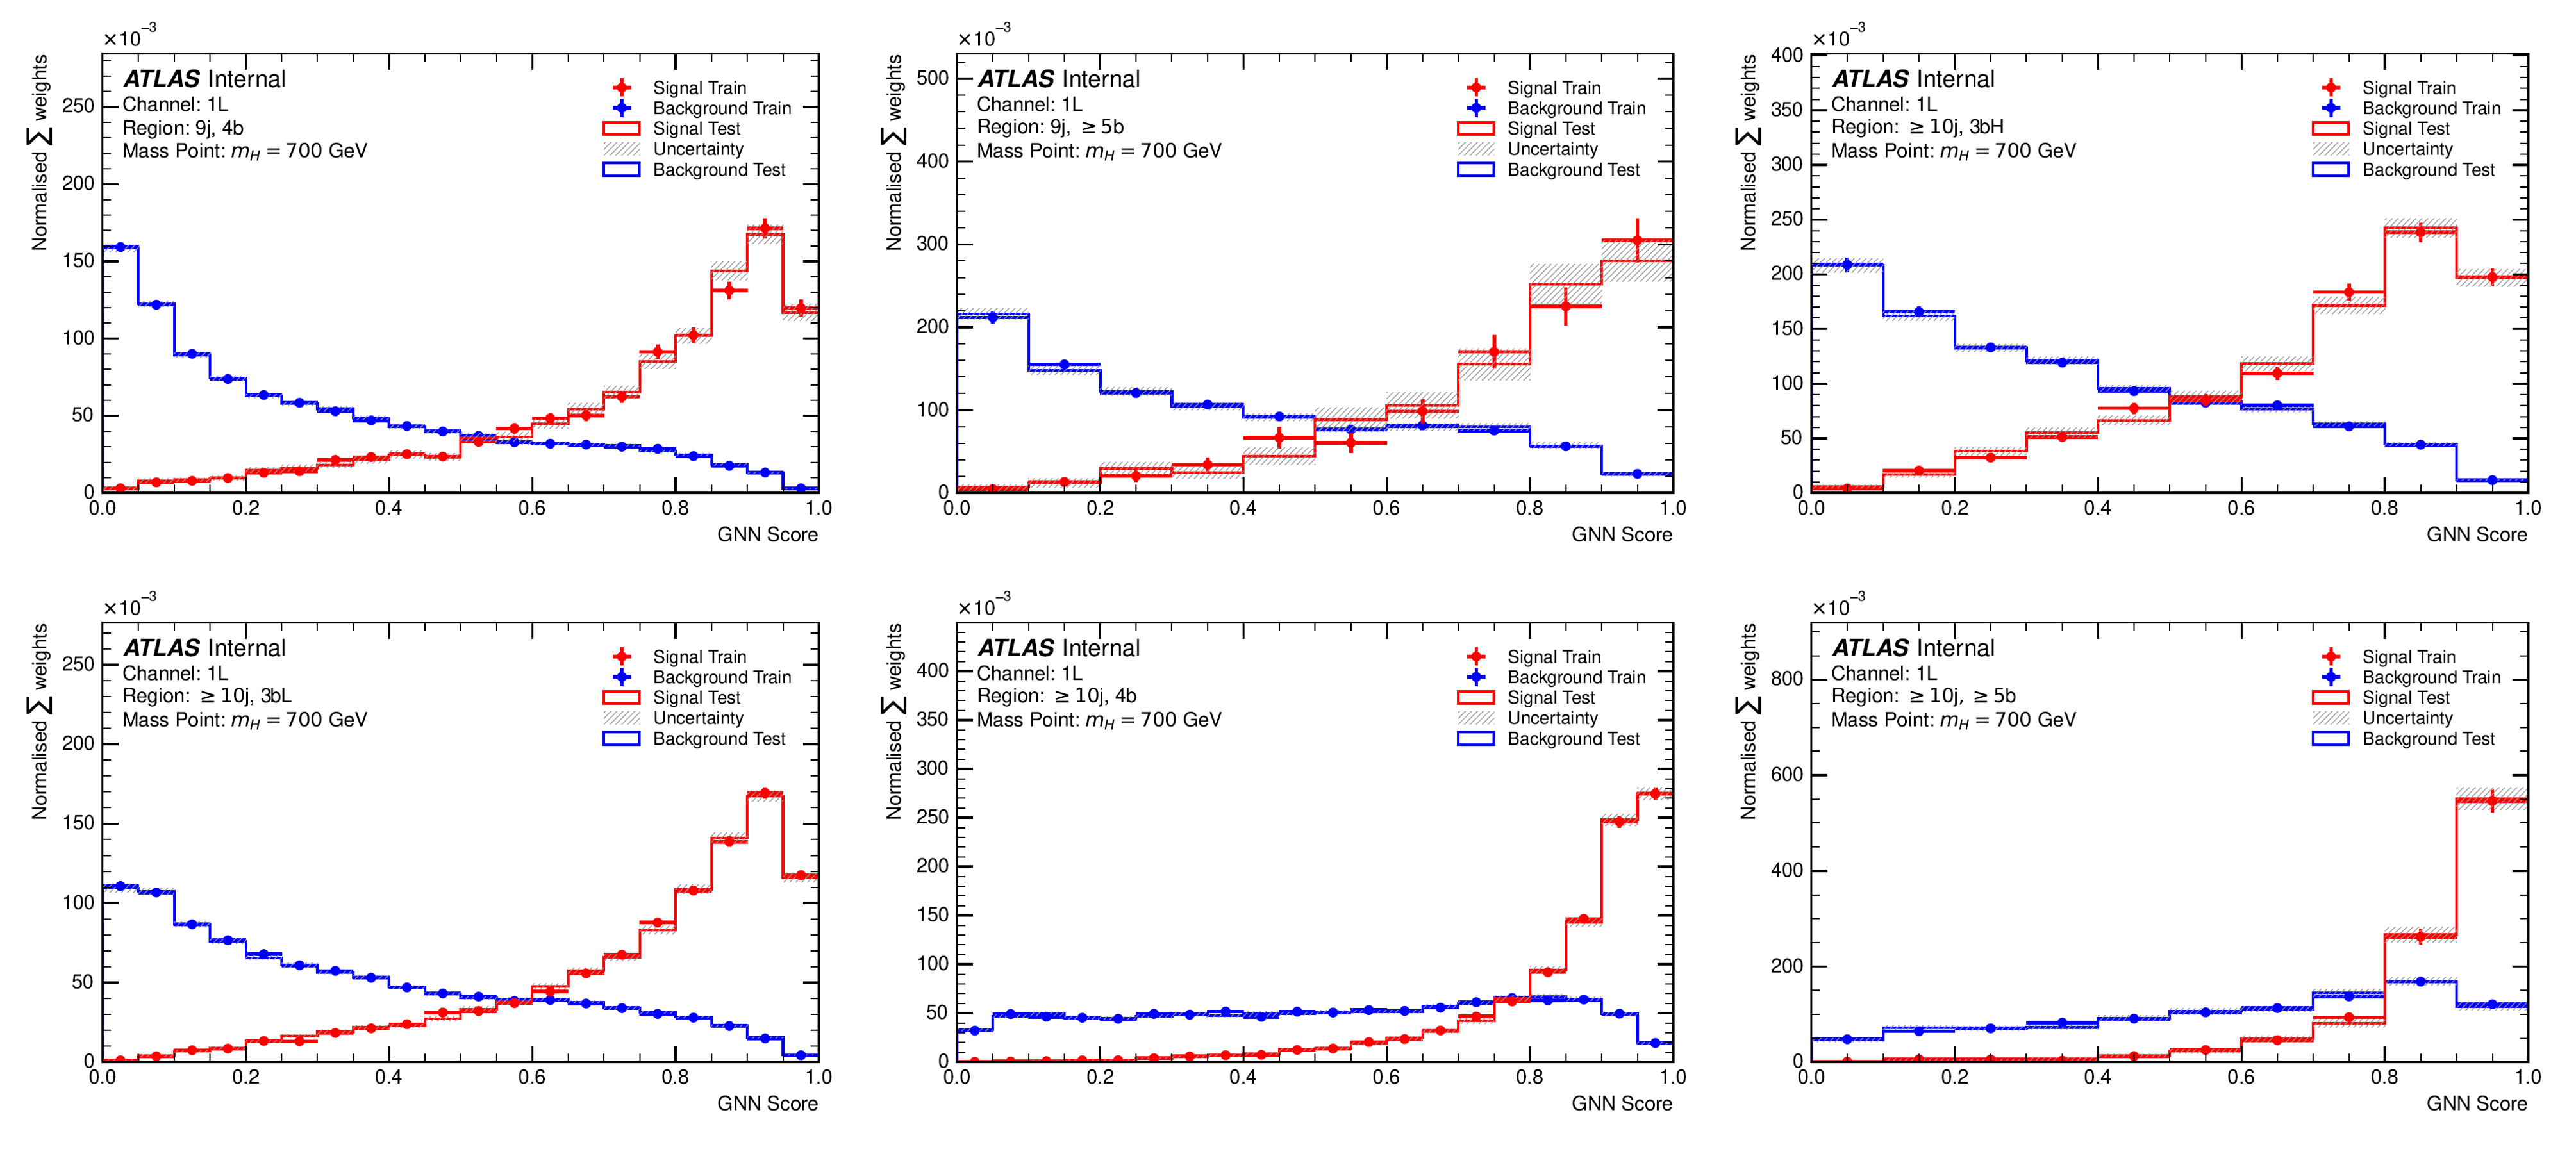
\includegraphics[width=0.48\textwidth]{figures/gnn/Plots_1L/700/GNN_Score_Plot_700GeV_Split.png}
        \caption{700 GeV mass point}
    \end{subfigure}
    \bigskip
    \centering
    \begin{subfigure}[t]{\textwidth}
        \centering
        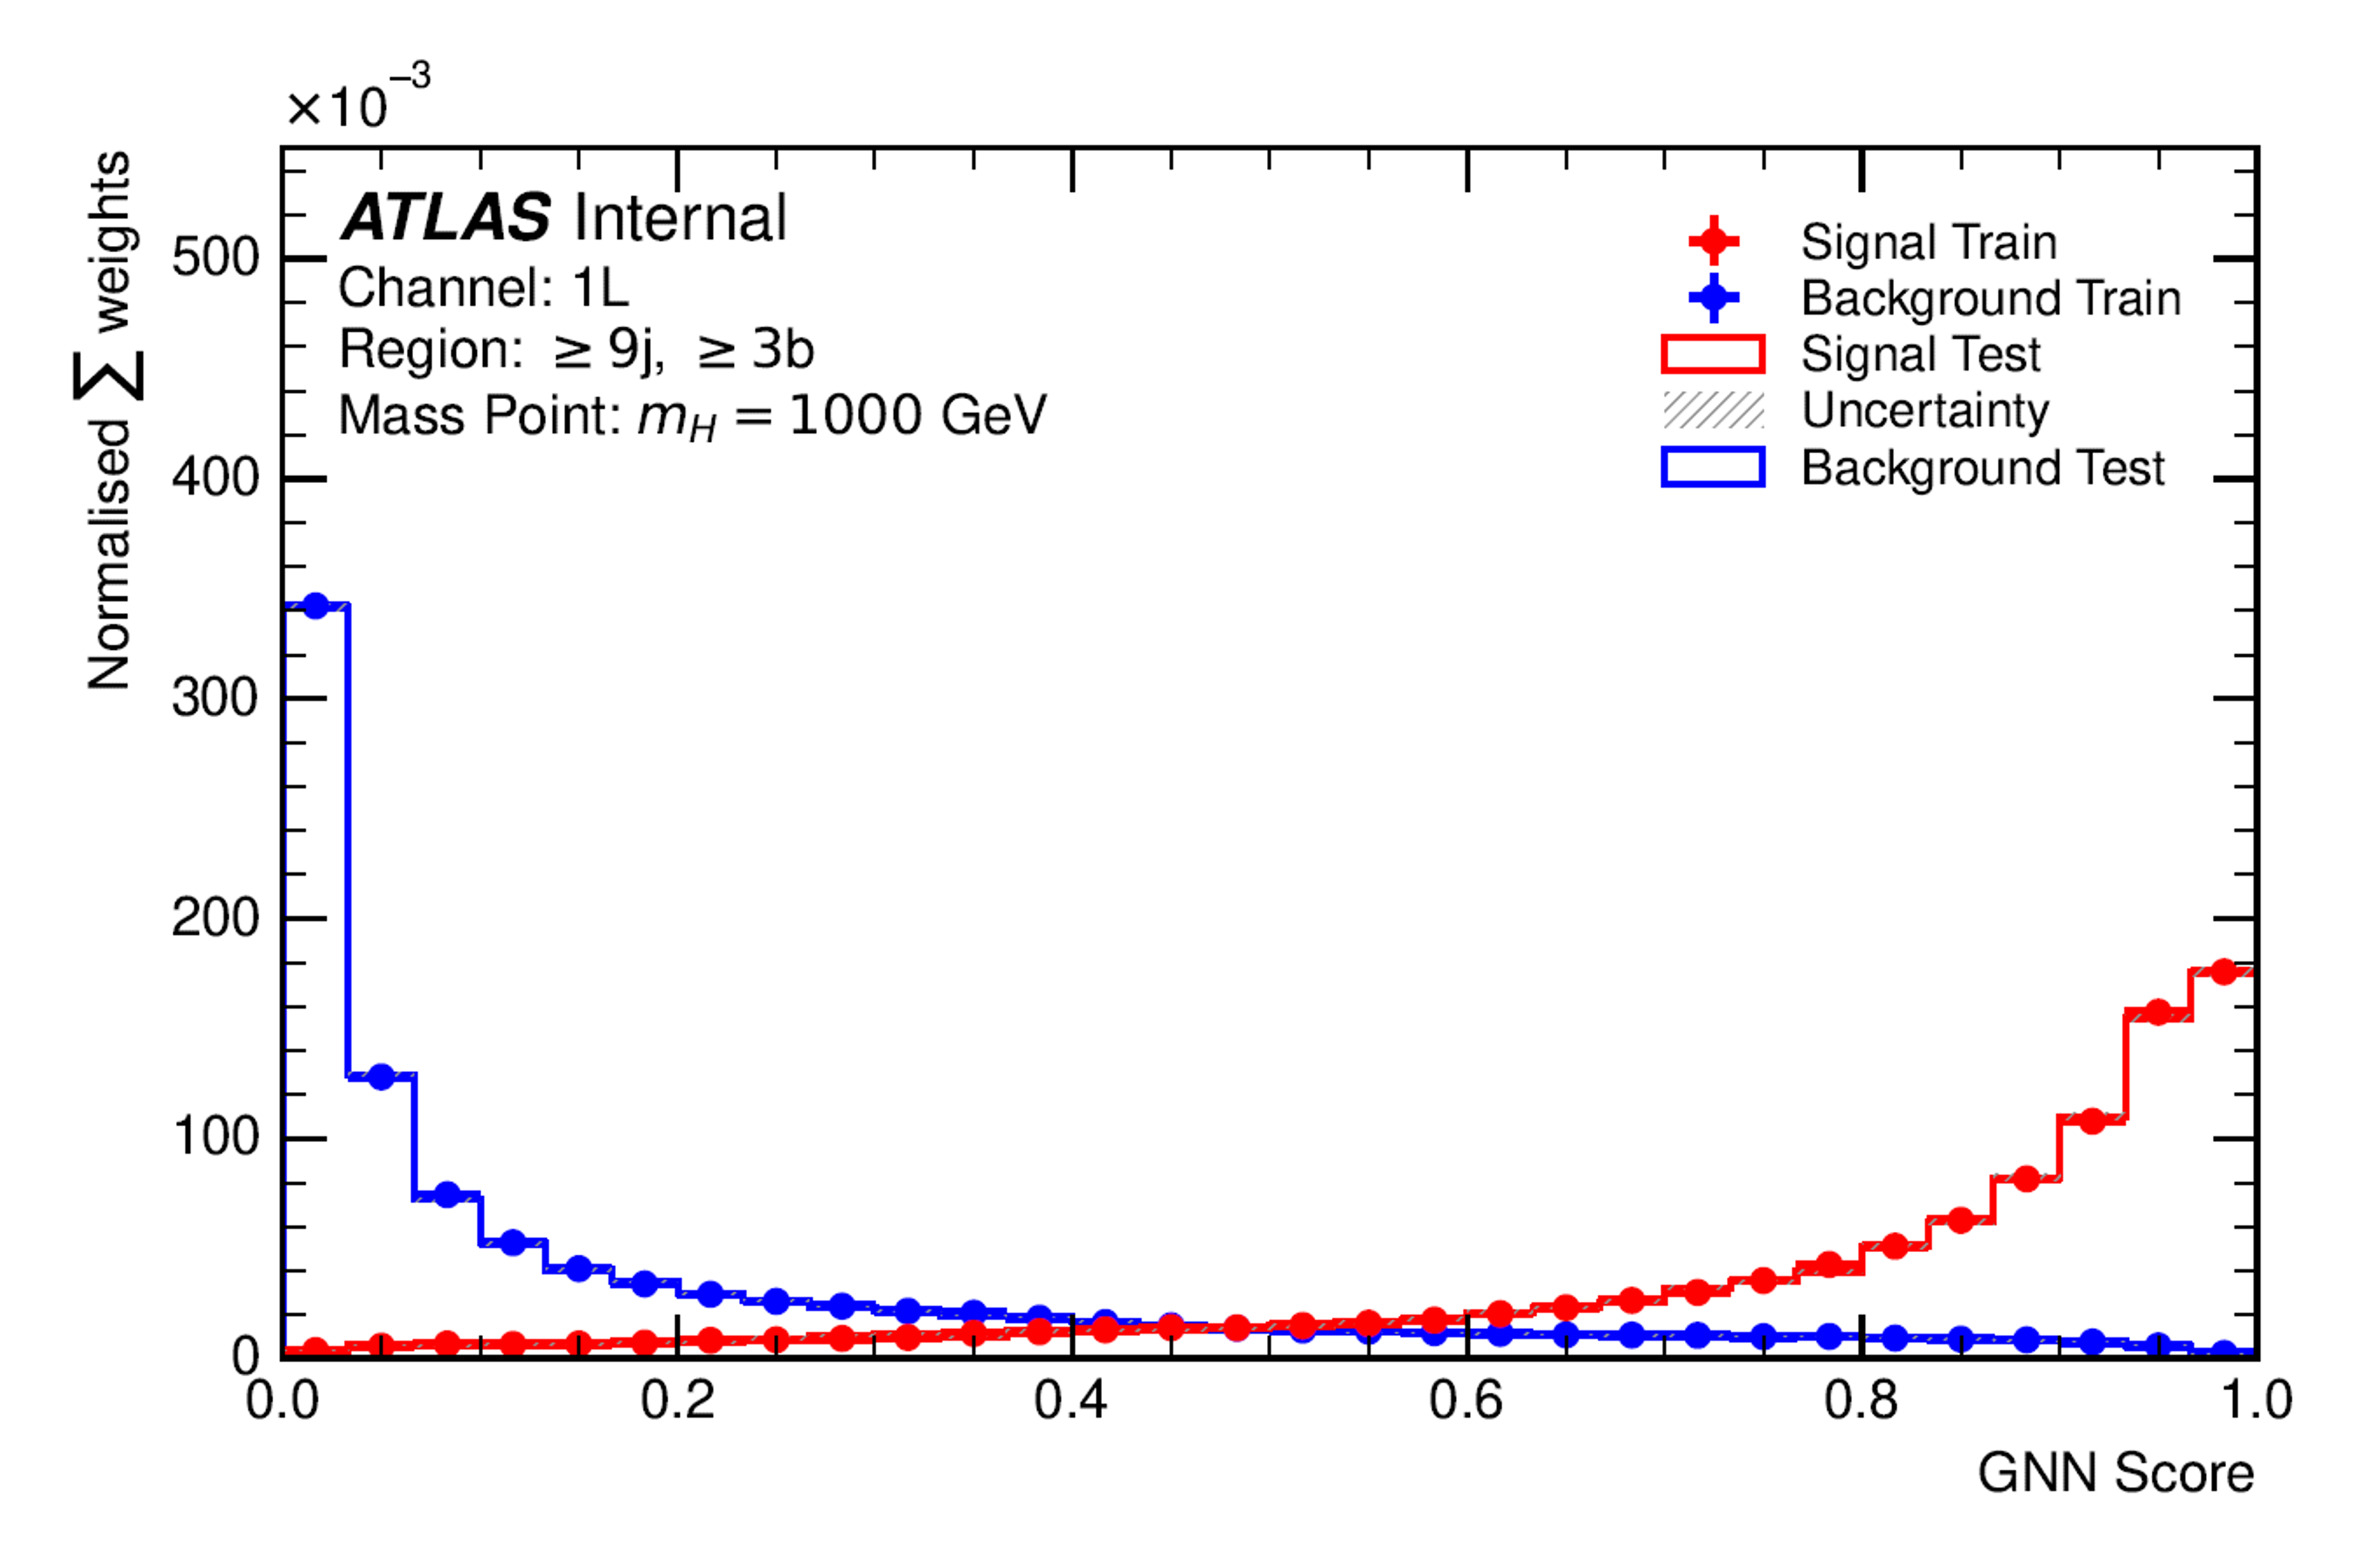
\includegraphics[width=0.48\textwidth]{figures/gnn/Plots_1L/1000/GNN_Score_Plot_1000GeV_Inclusive.png}
        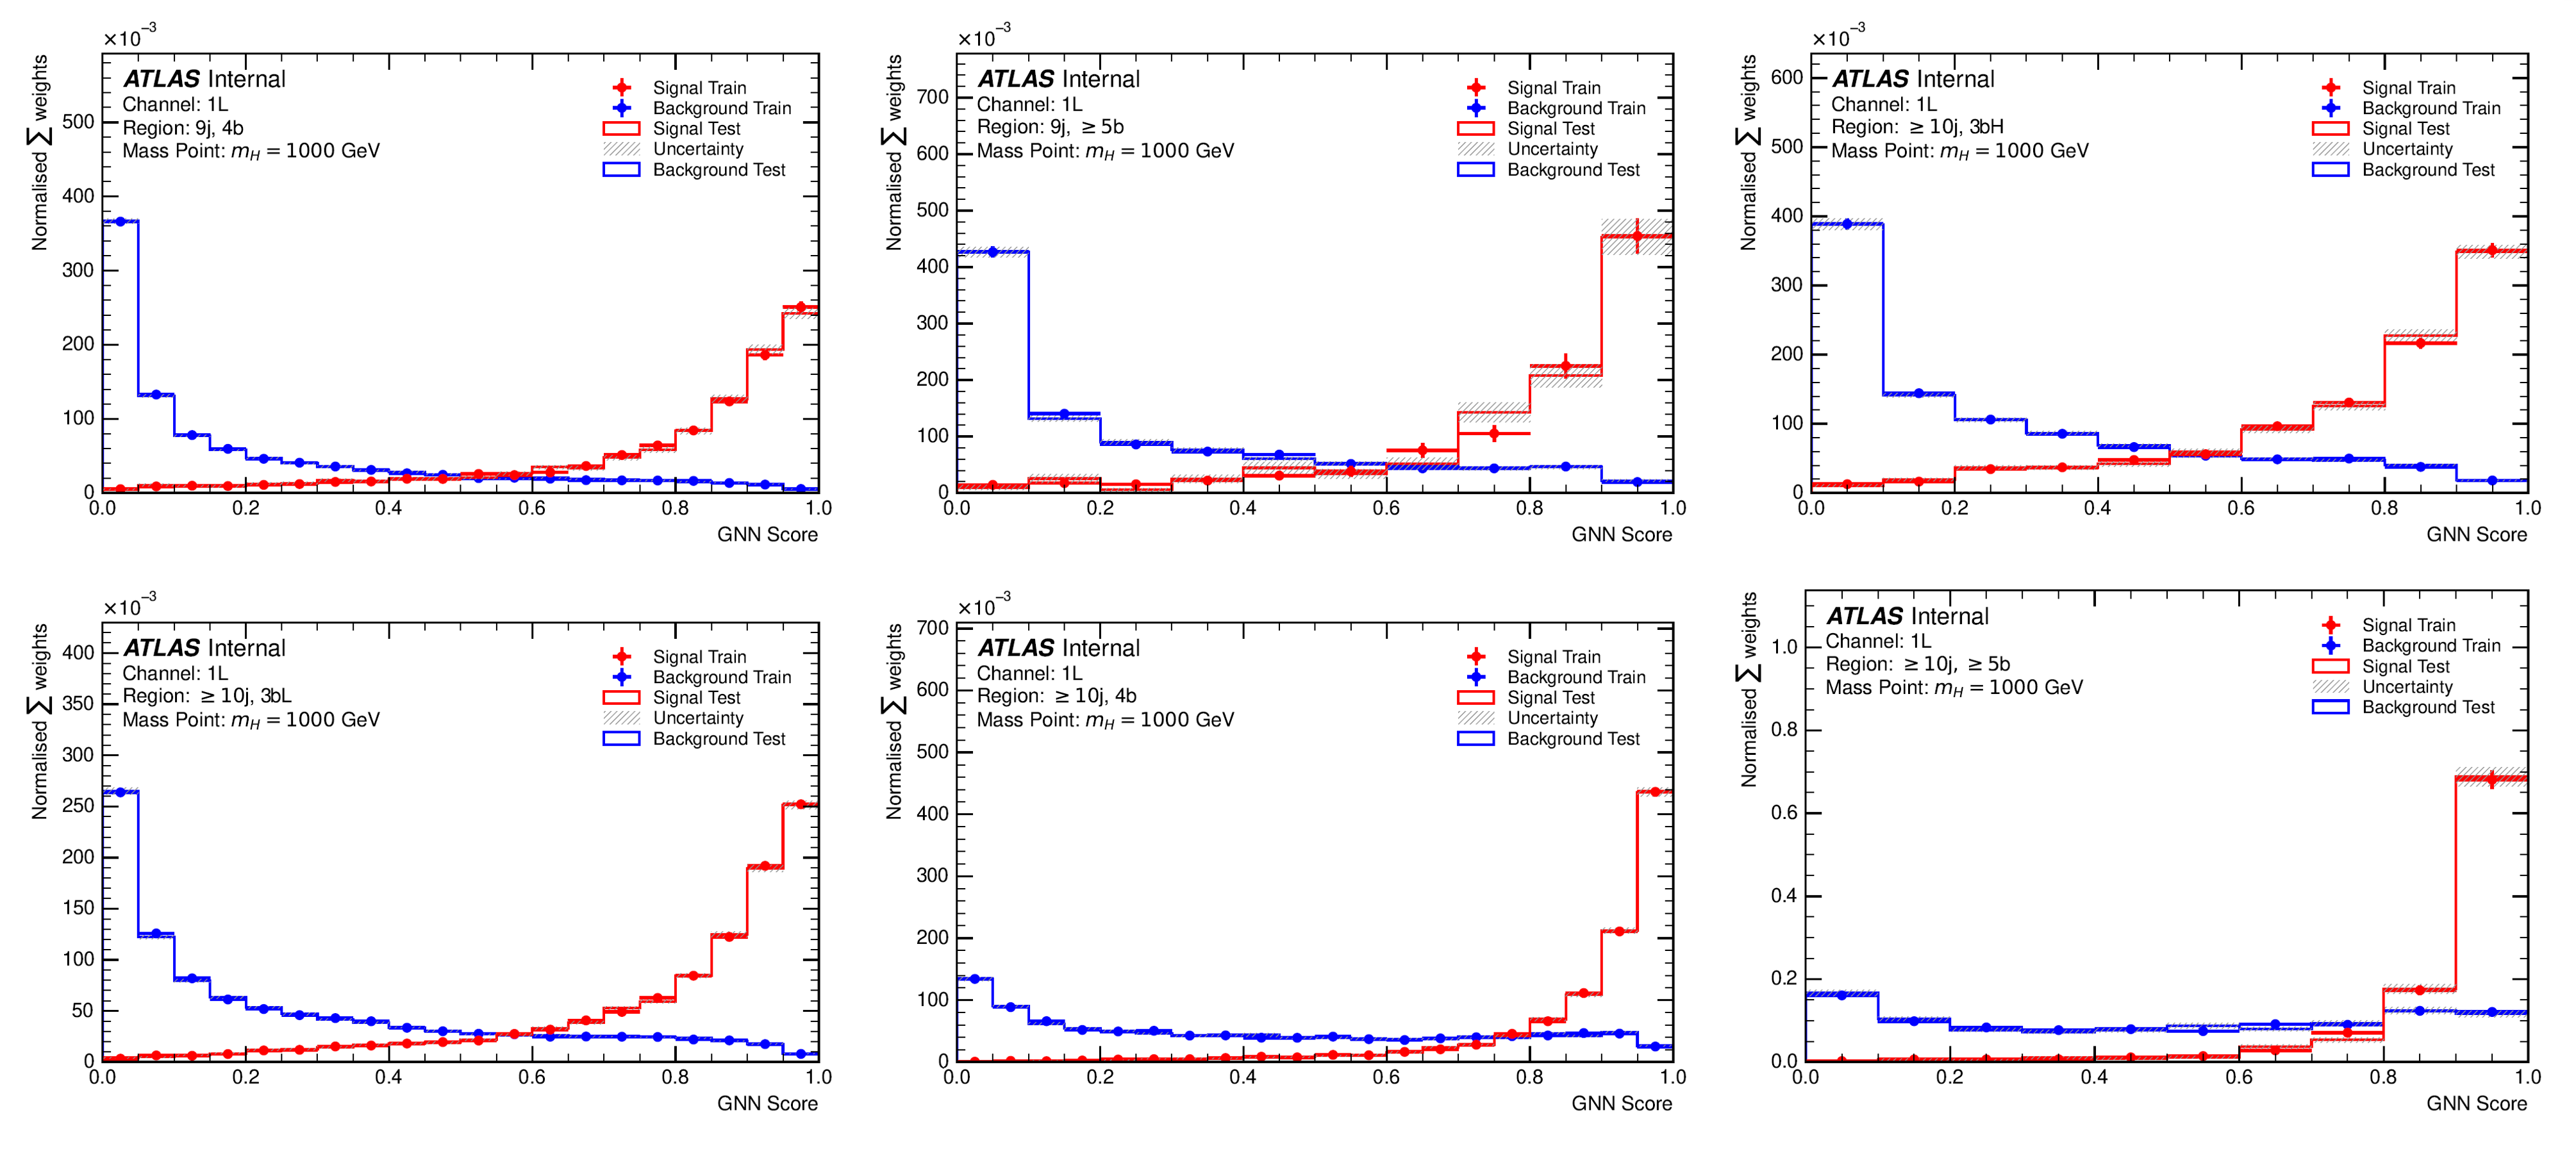
\includegraphics[width=0.48\textwidth]{figures/gnn/Plots_1L/1000/GNN_Score_Plot_1000GeV_Split.png}
        \caption{1000 GeV mass point}
    \end{subfigure}
    \caption{Score distributions for the 1L GNN for several mass points. Shown in the inclusive training region (left) and four subdivided regions (right). Distributions are shown separately for models trained on even/odd event numbers and are split into training and testing results. The combined result of the cross trained model is shown in blue (signal) and red (background).}
    \label{fig:1l-gnn-scores}
\end{figure} 


\begin{figure}[h!]
    \centering
    \begin{subfigure}[t]{\textwidth}
        \centering
        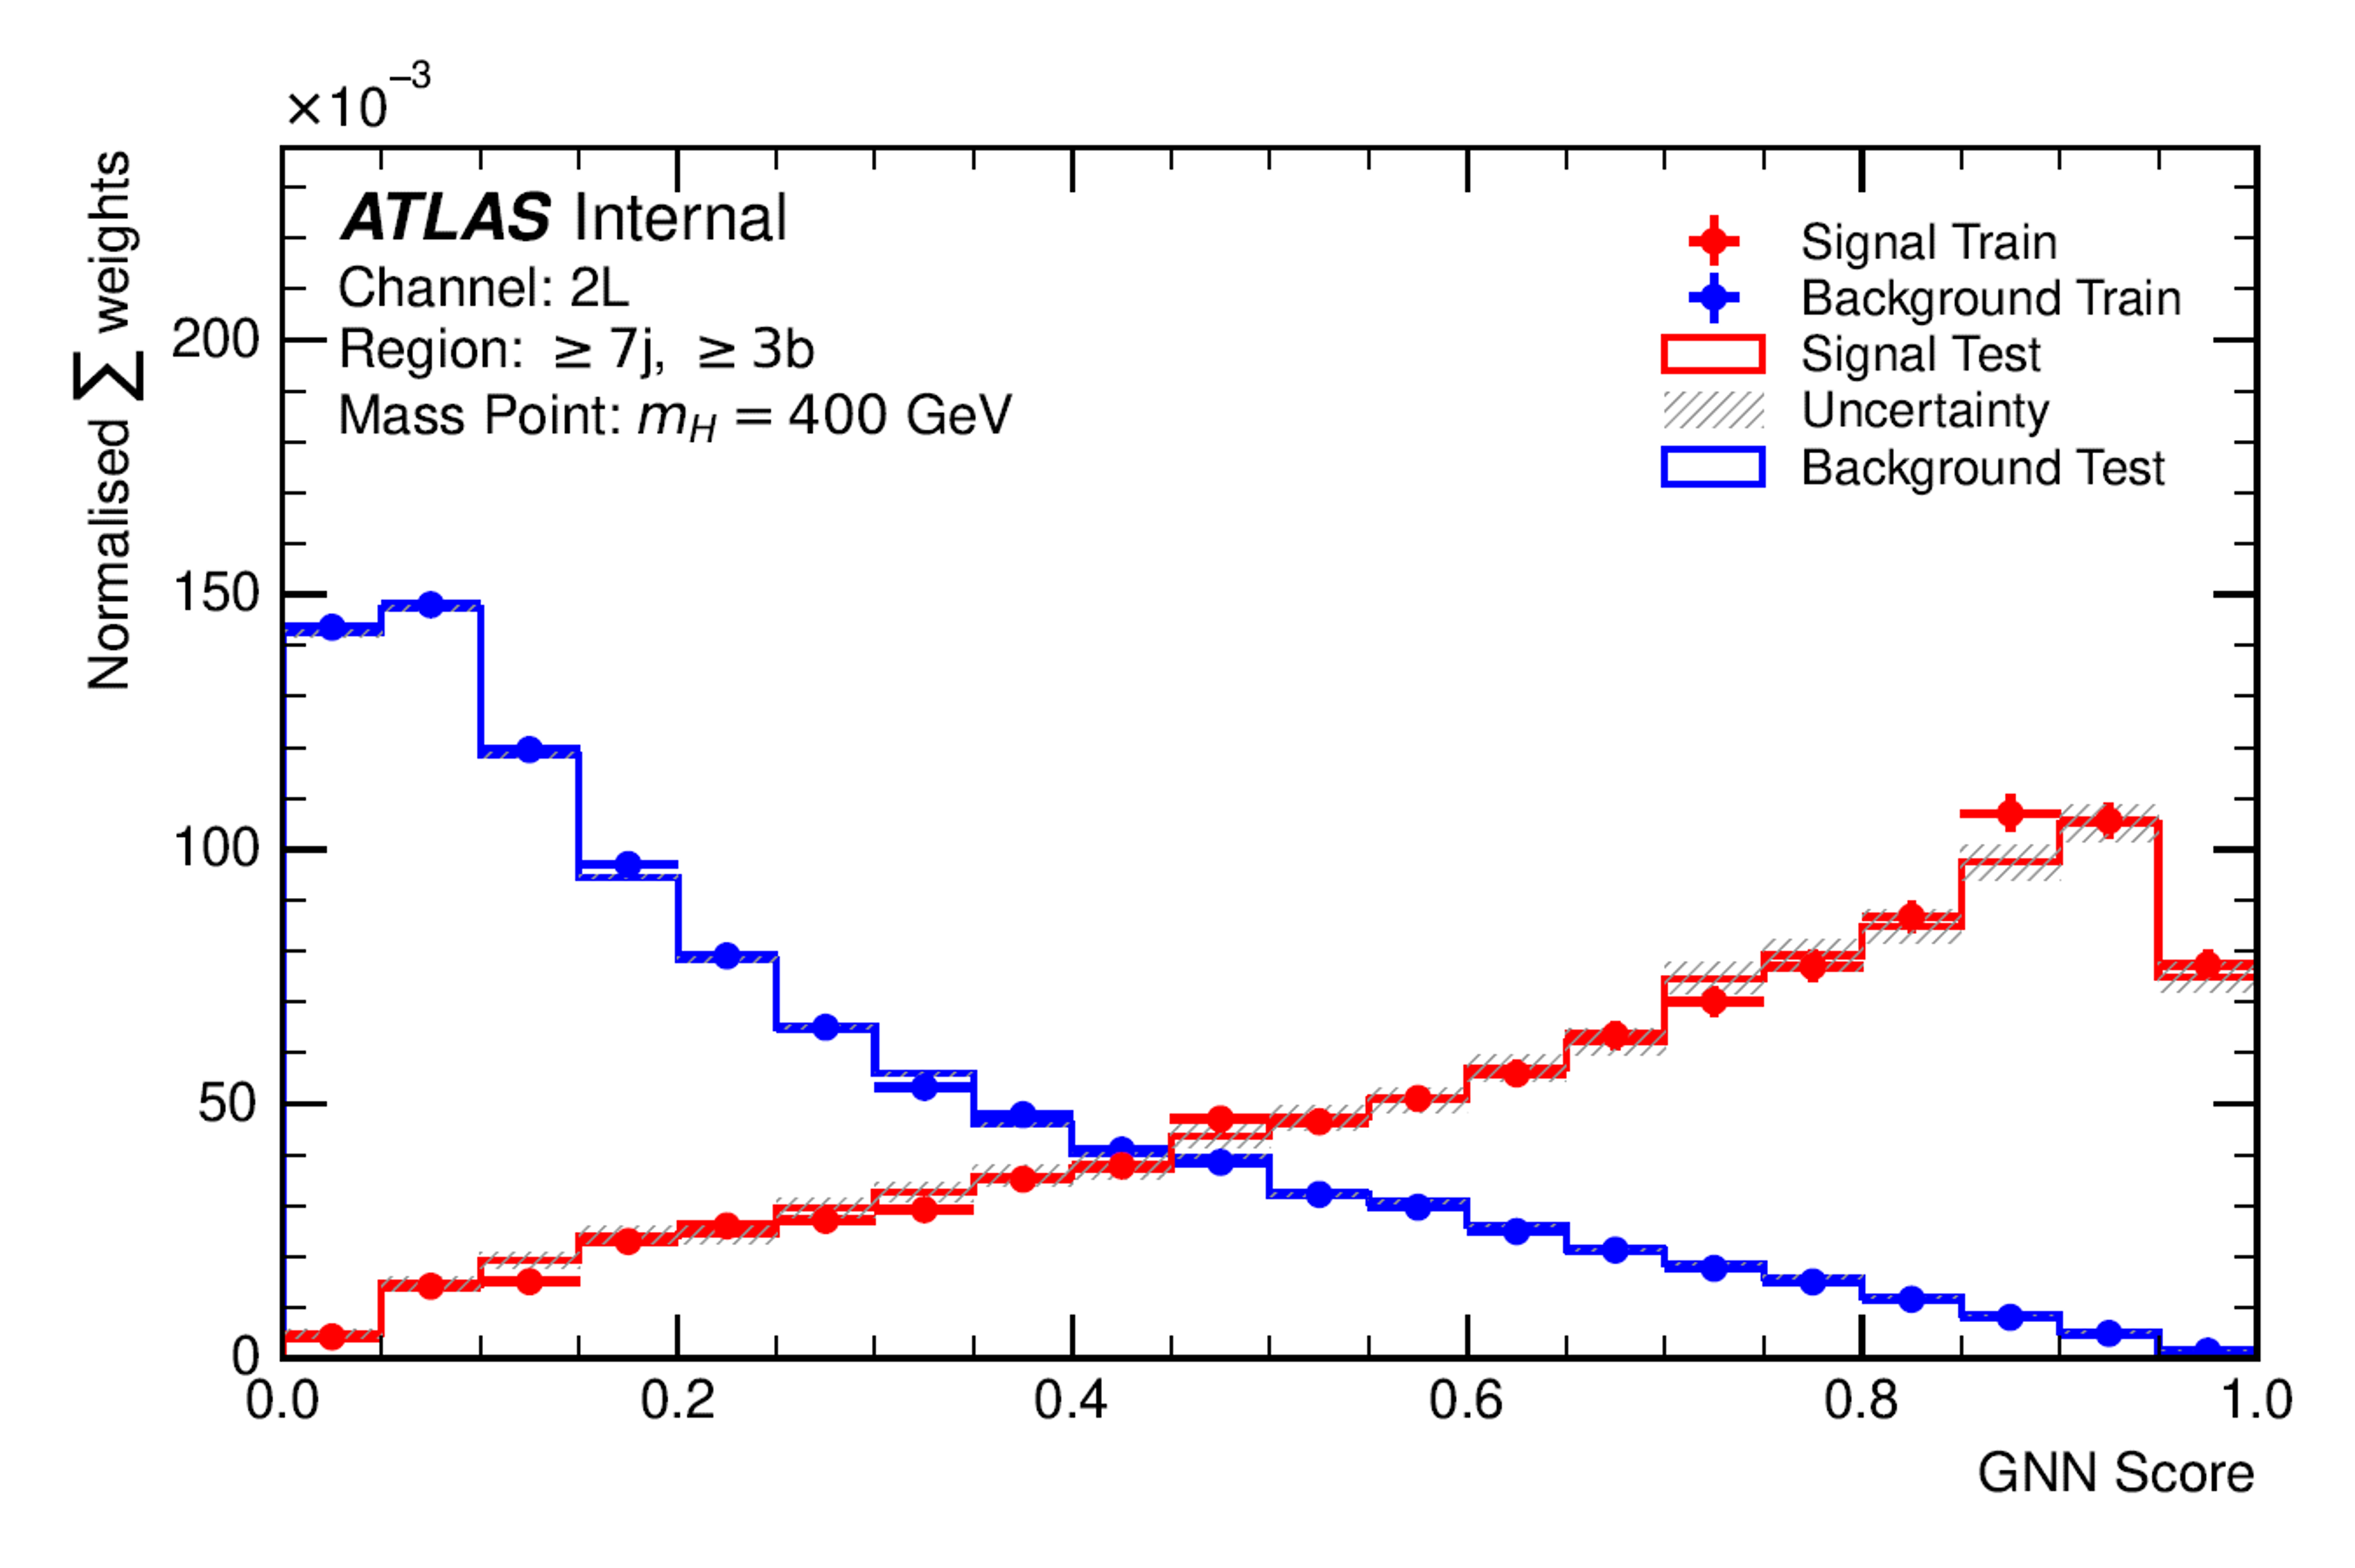
\includegraphics[width=0.48\textwidth]{figures/gnn/Plots_2LOS/400/GNN_Score_Plot_400GeV_Inclusive.png}
        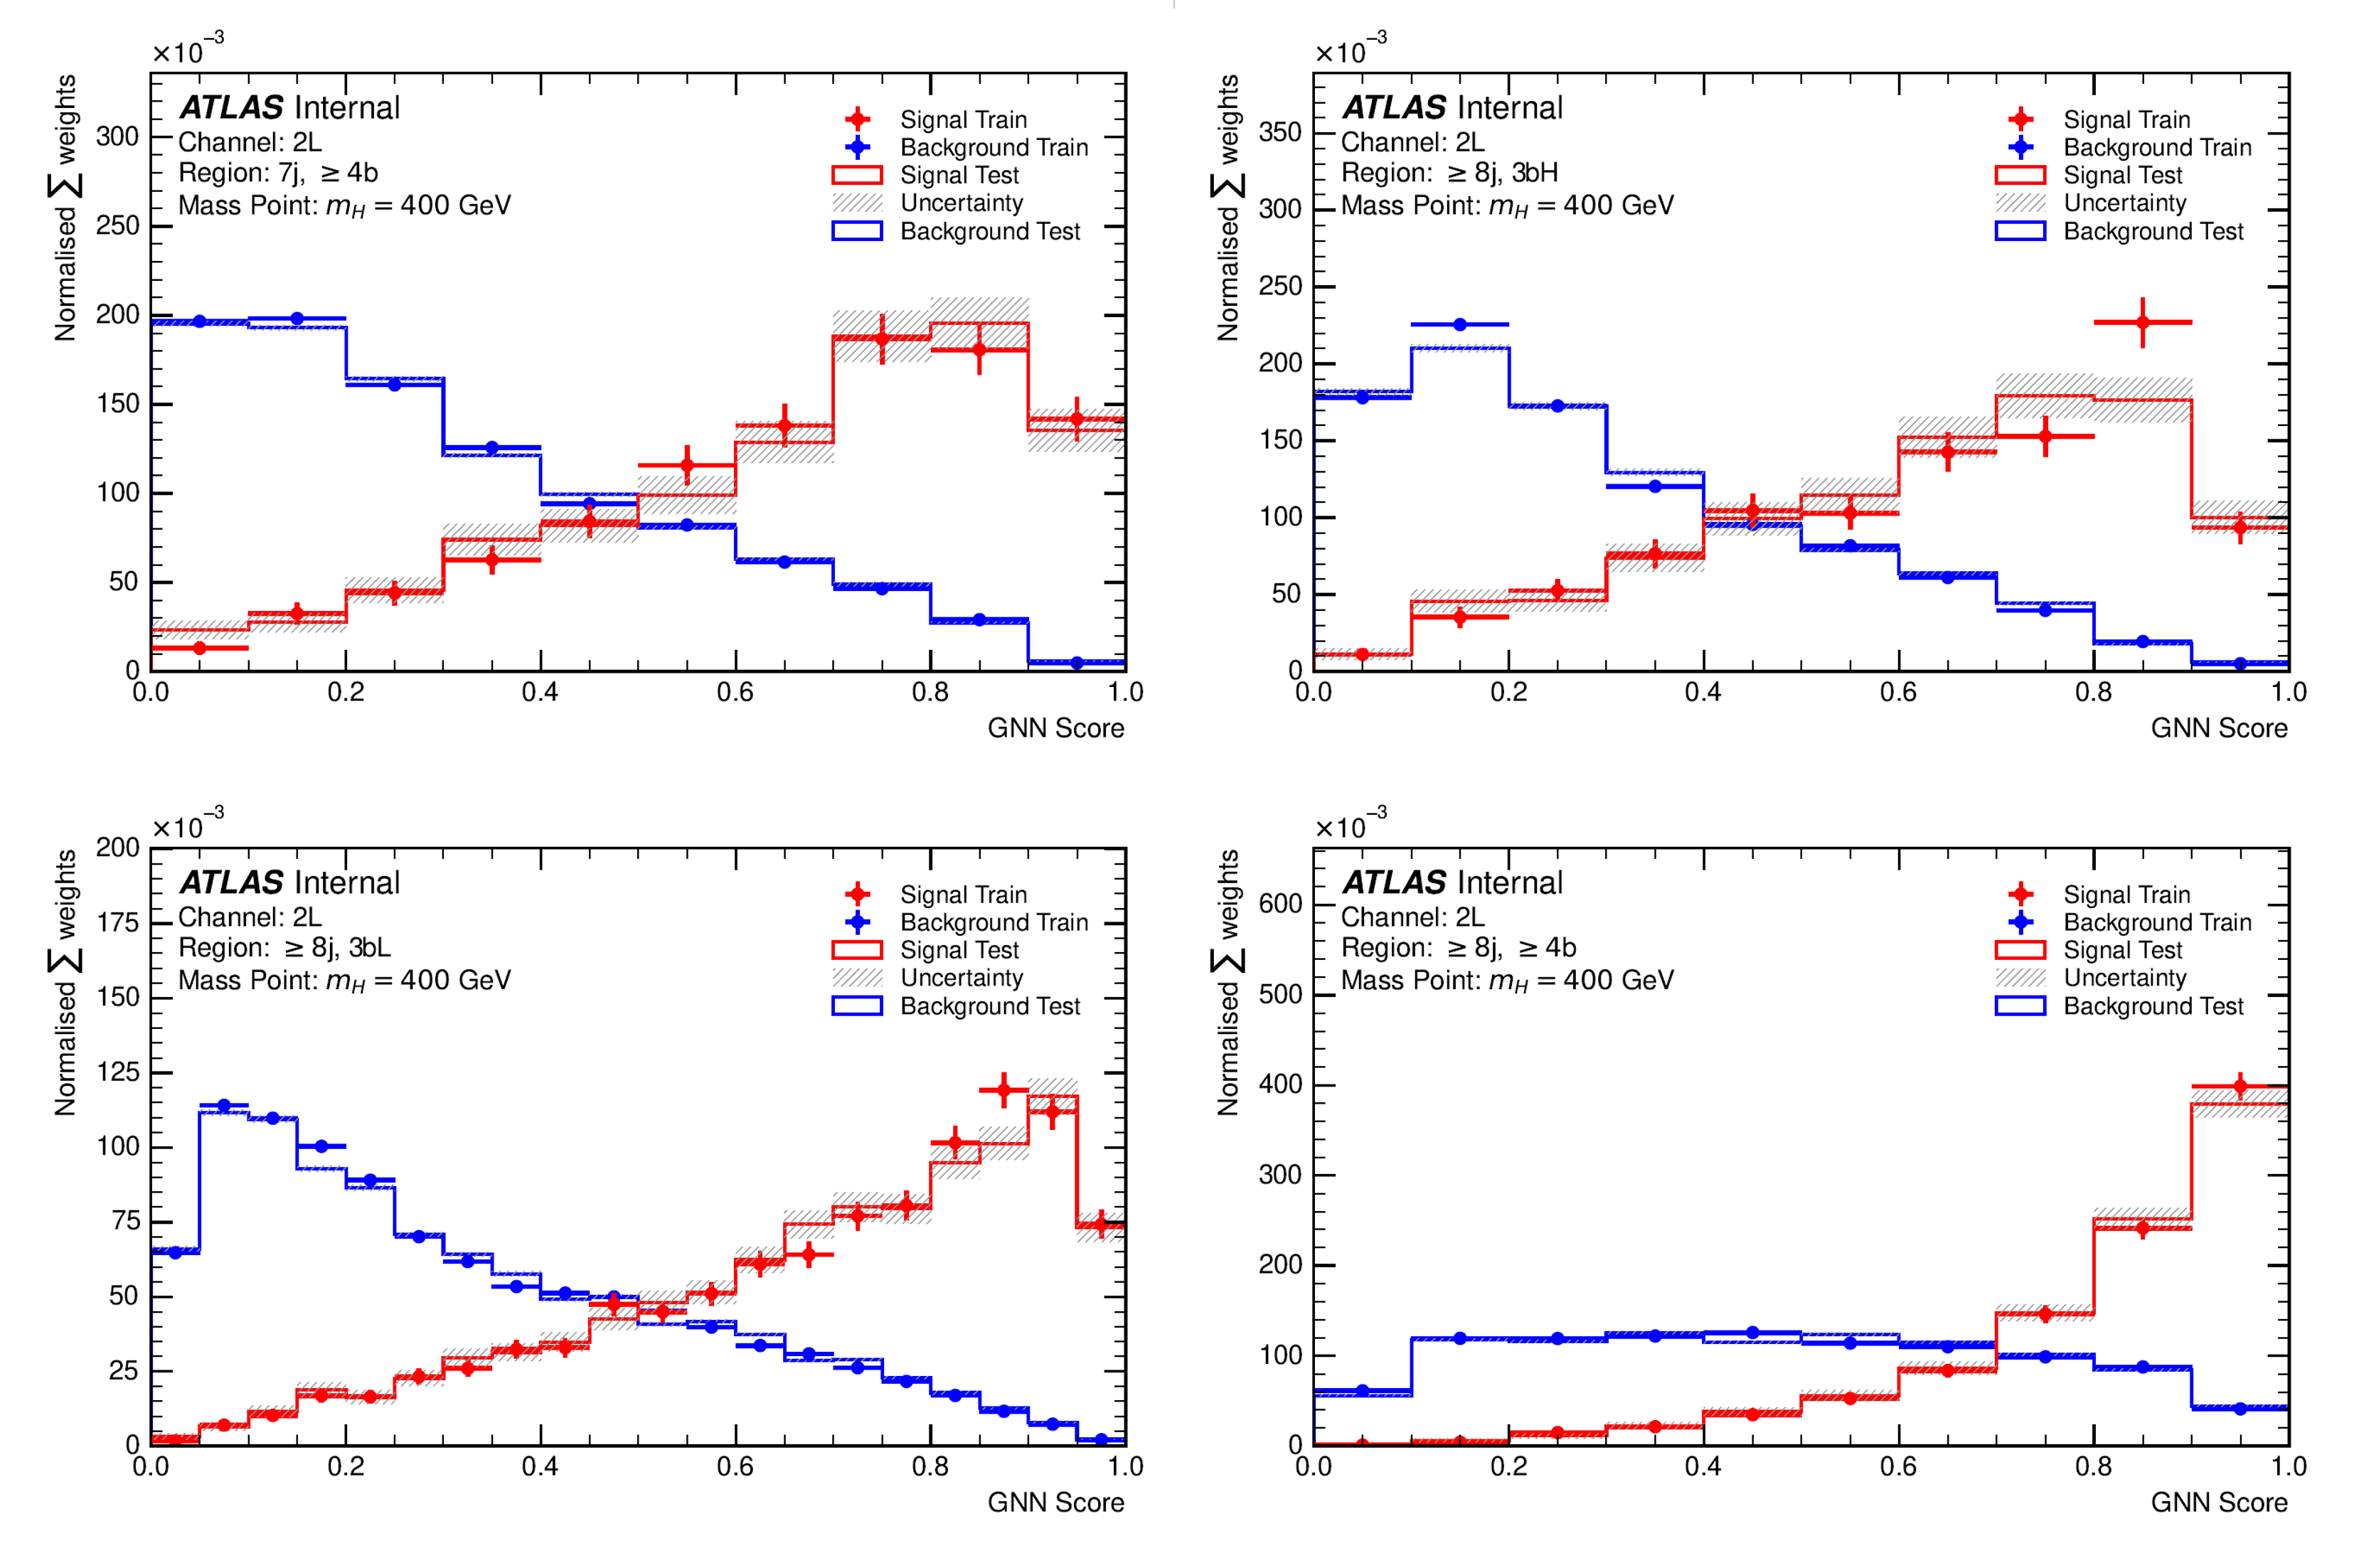
\includegraphics[width=0.48\textwidth]{figures/gnn/Plots_2LOS/400/GNN_Score_Plot_400GeV_Split.png}
        \caption{400 GeV mass point}
    \end{subfigure}
    \bigskip
    \centering
    \begin{subfigure}[t]{\textwidth}
        \centering
        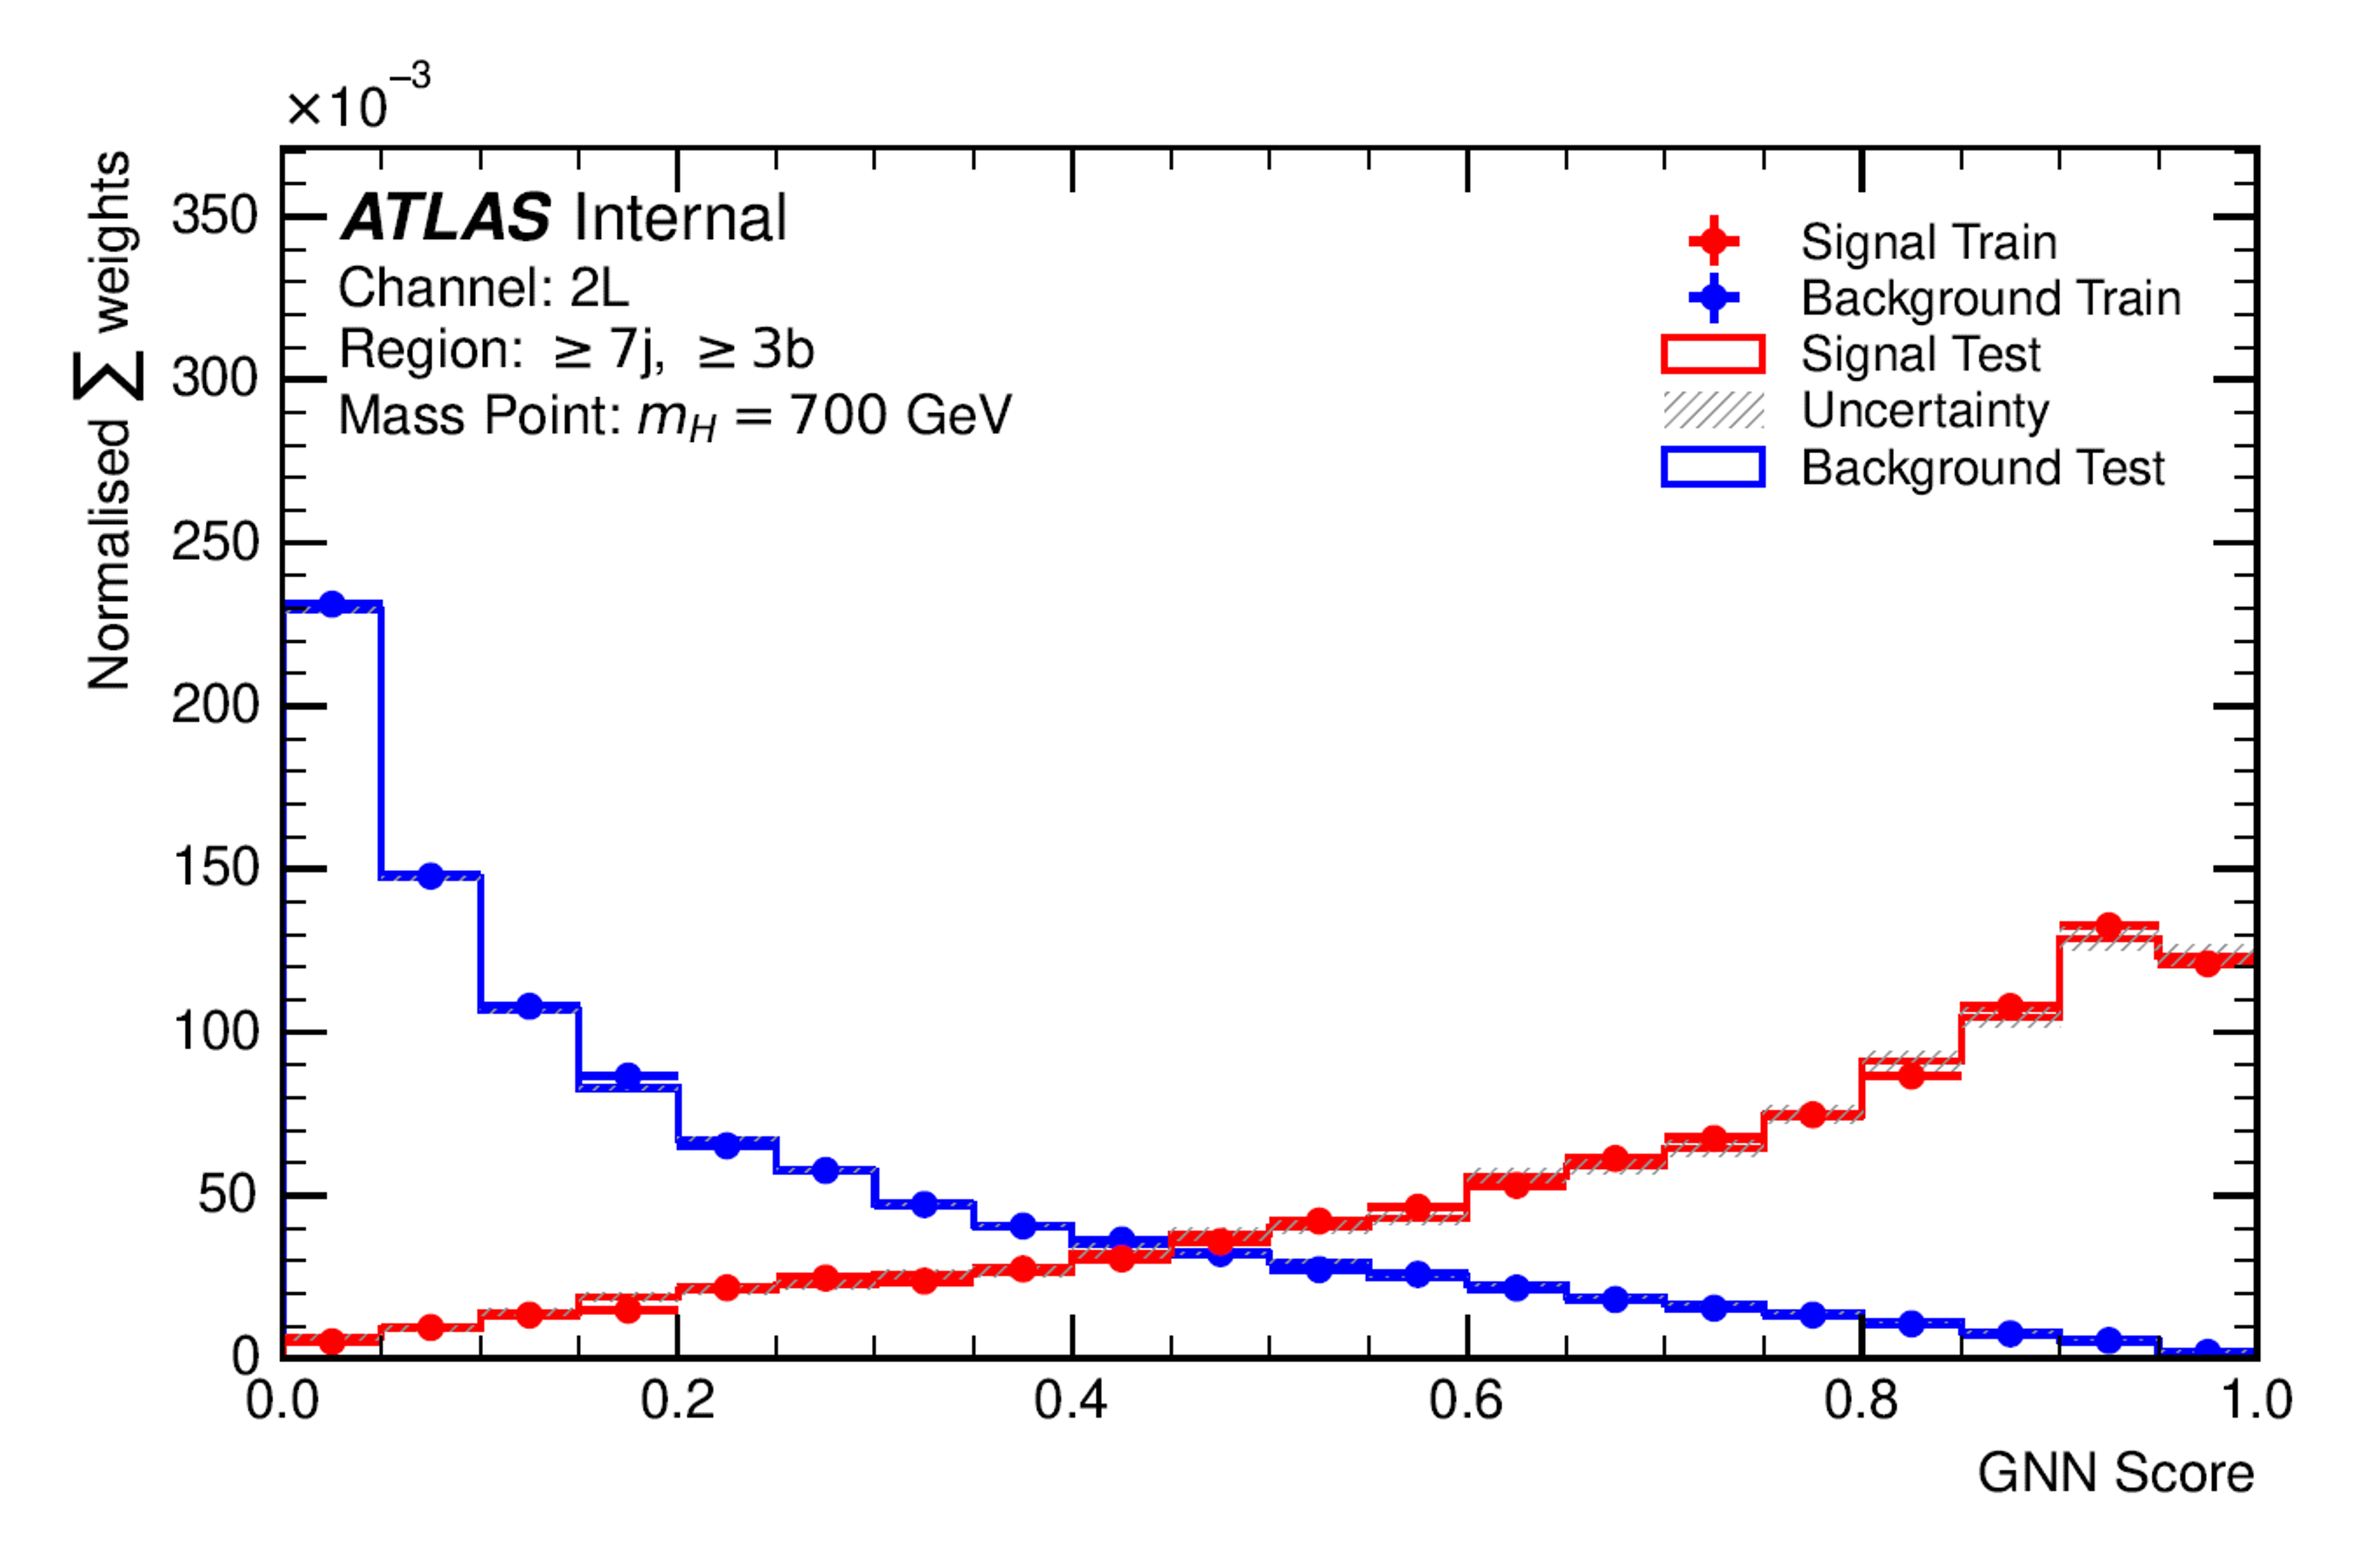
\includegraphics[width=.48\textwidth]{figures/gnn/Plots_2LOS/700/GNN_Score_Plot_700GeV_Inclusive.png}
        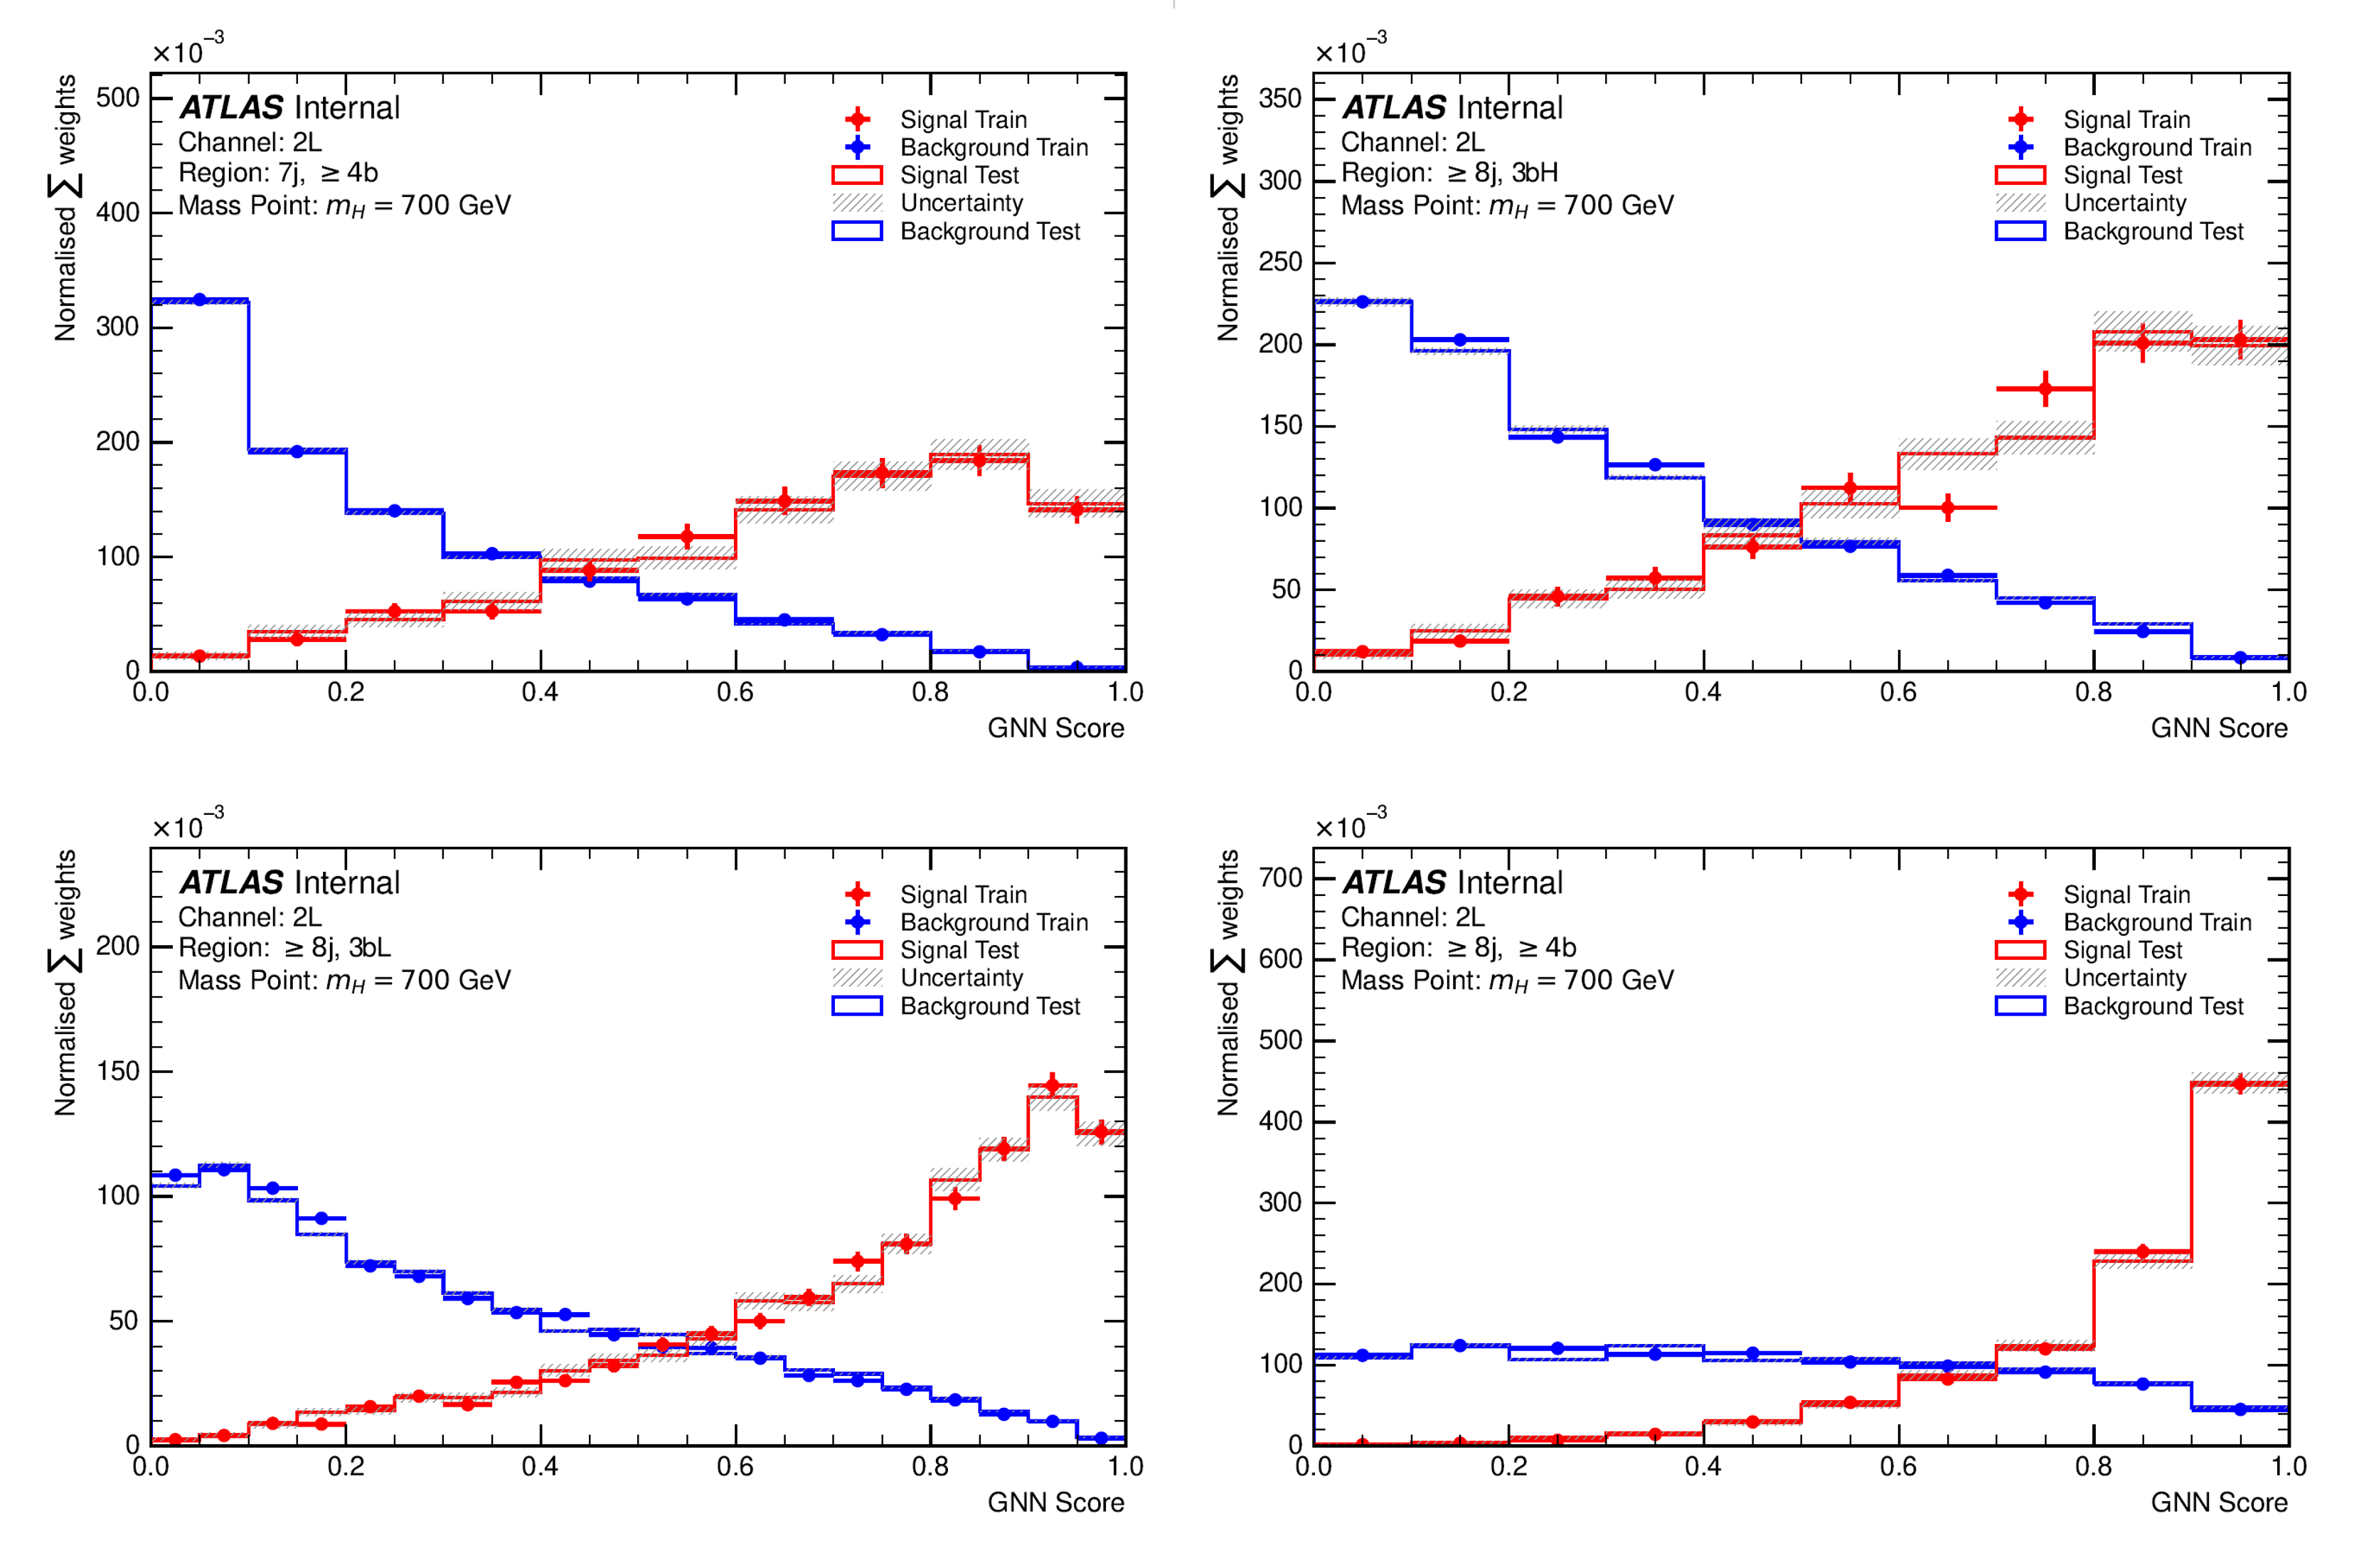
\includegraphics[width=.48\textwidth]{figures/gnn/Plots_2LOS/700/GNN_Score_Plot_700GeV_Split.png}
        \caption{700 GeV mass point}
    \end{subfigure}
    \bigskip
    \centering
    \begin{subfigure}[t]{\textwidth}
        \centering
        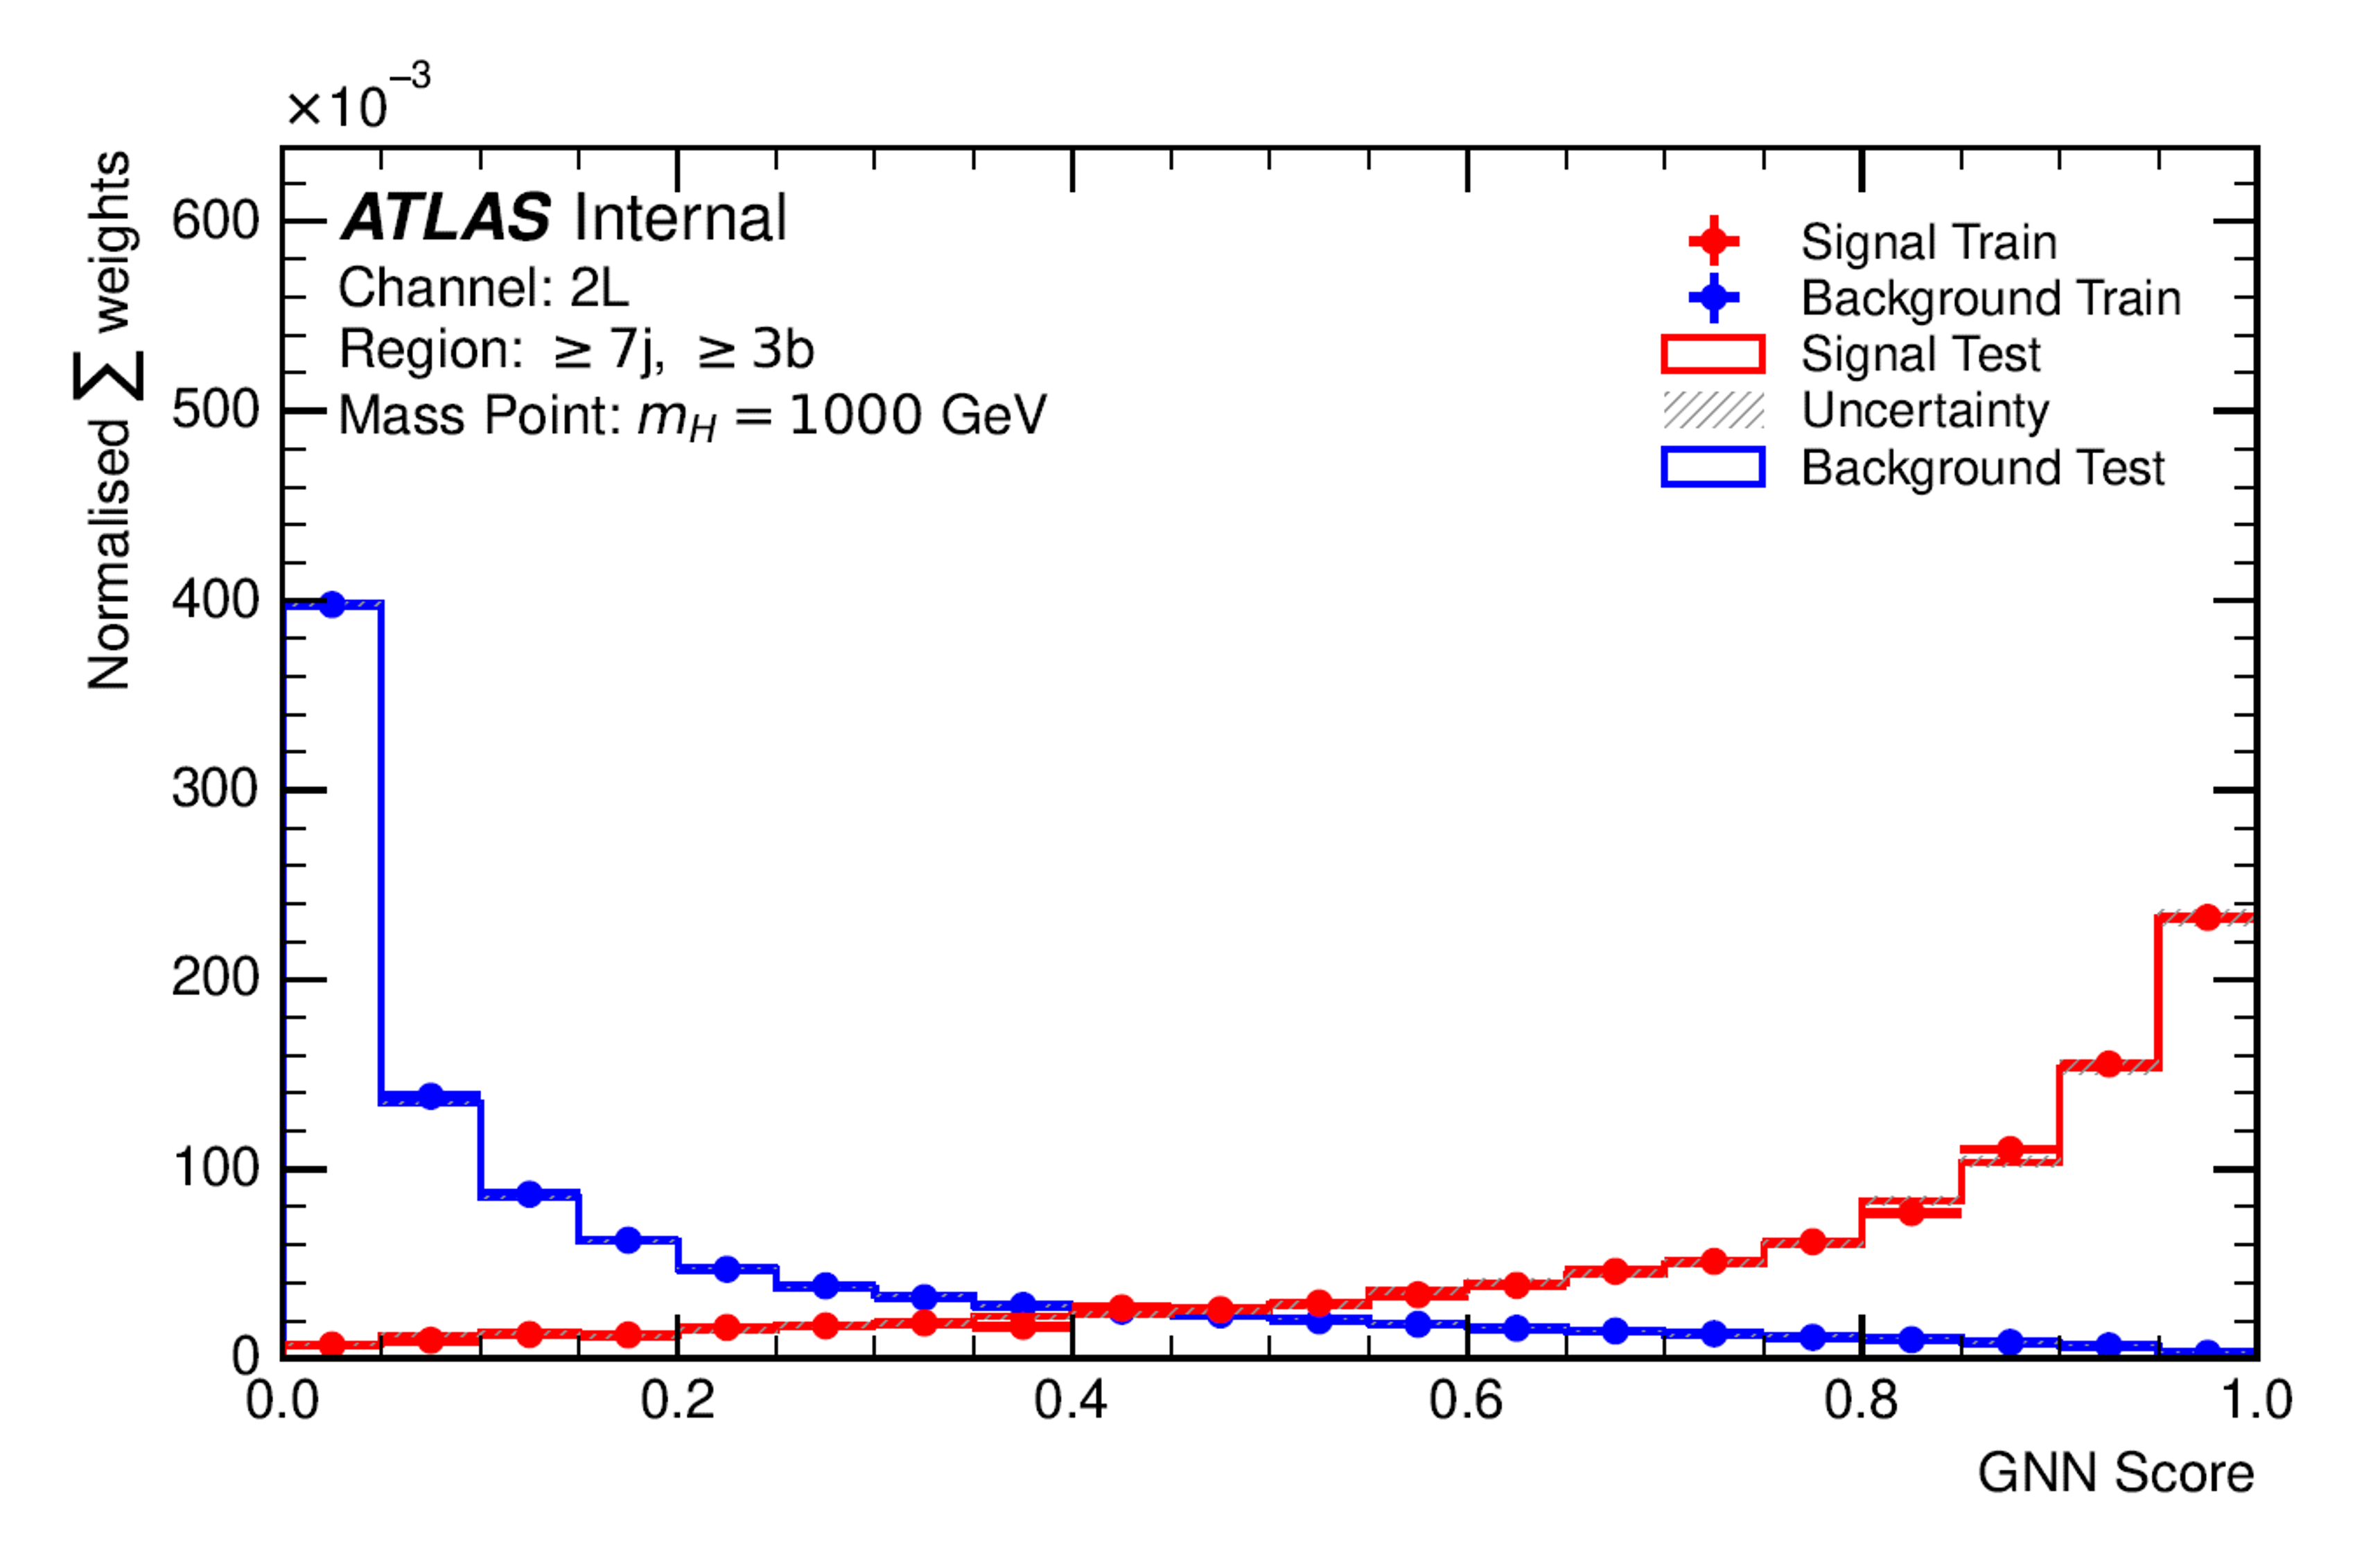
\includegraphics[width=.48\textwidth]{figures/gnn/Plots_2LOS/1000/GNN_Score_Plot_1000GeV_Inclusive.png}
        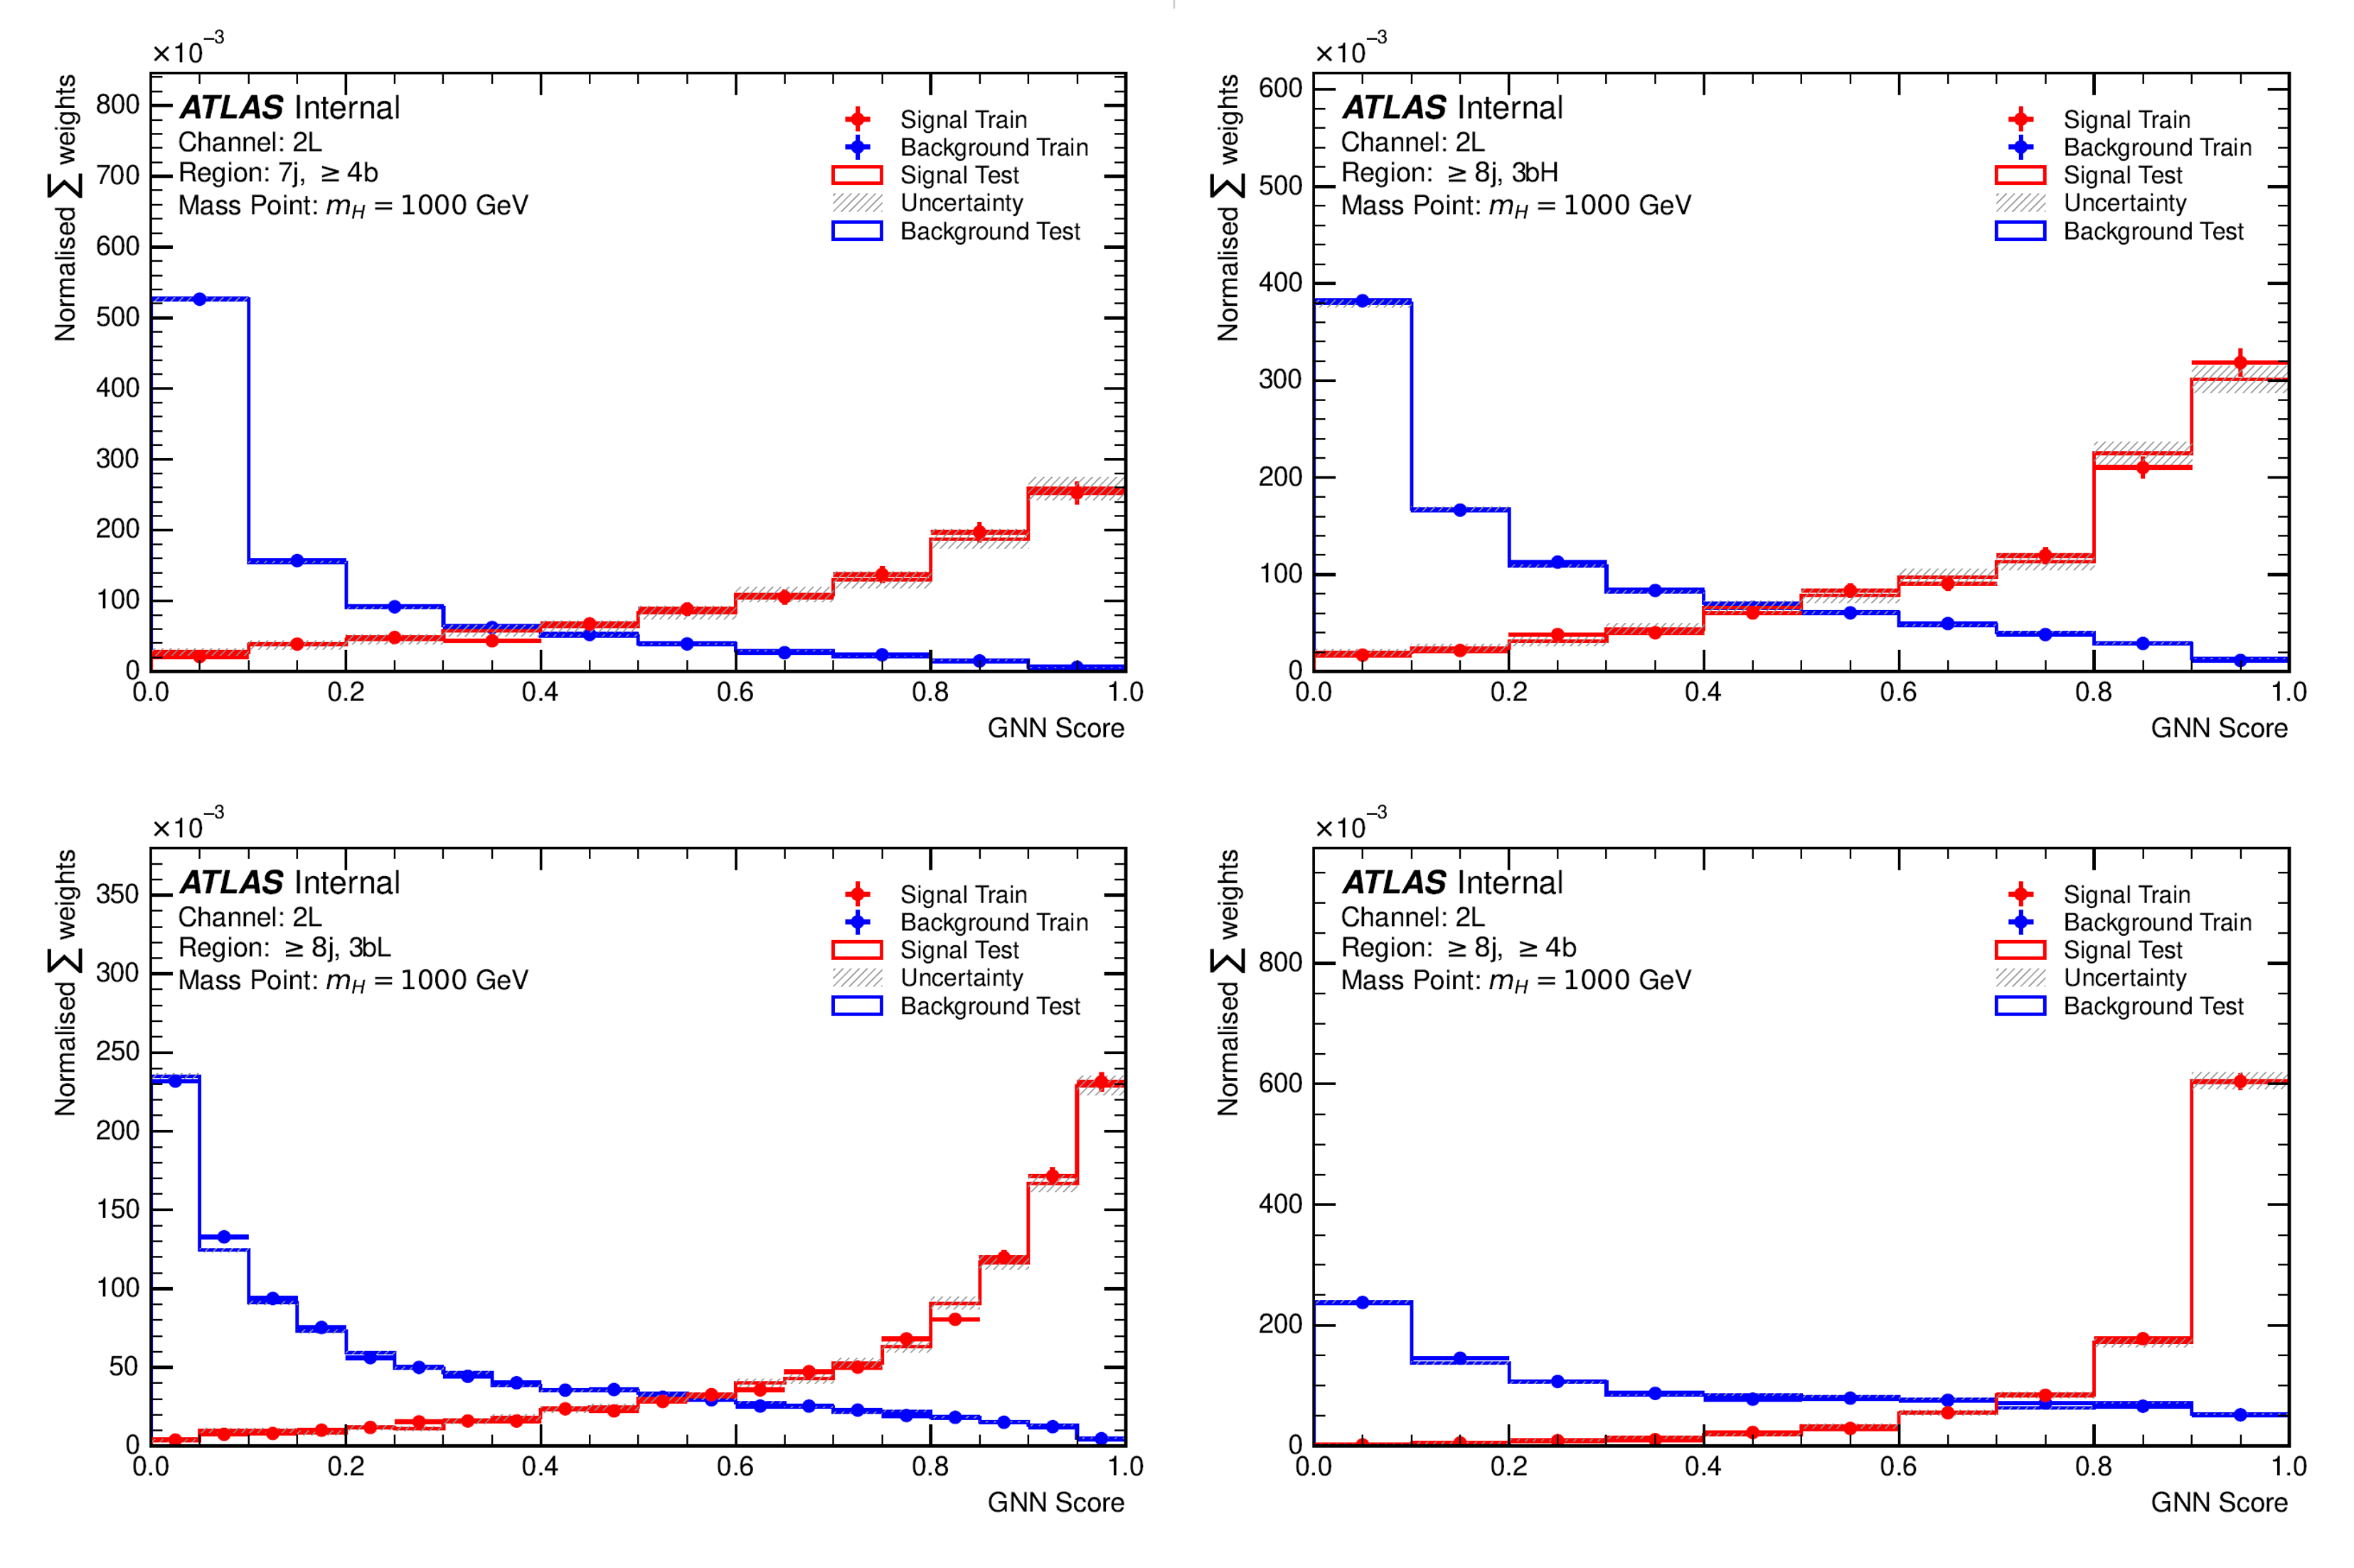
\includegraphics[width=.48\textwidth]{figures/gnn/Plots_2LOS/1000/GNN_Score_Plot_1000GeV_Split.png}
        \caption{1000 GeV mass point}
    \end{subfigure}
    \caption{Score distributions for the 2LOS GNN for several mass points. Shown in the inclusive training region (left) and four subdivided regions (right). Distributions are shown separately for models trained on even/odd event numbers and are split into training and testing results. The combined result of the cross trained model is shown in blue (signal) and red (background).}
    \label{fig:2los-gnn-scores}
\end{figure}

\begin{figure}[h!]
    \centering
    \begin{subfigure}[t]{\textwidth}
        \centering
        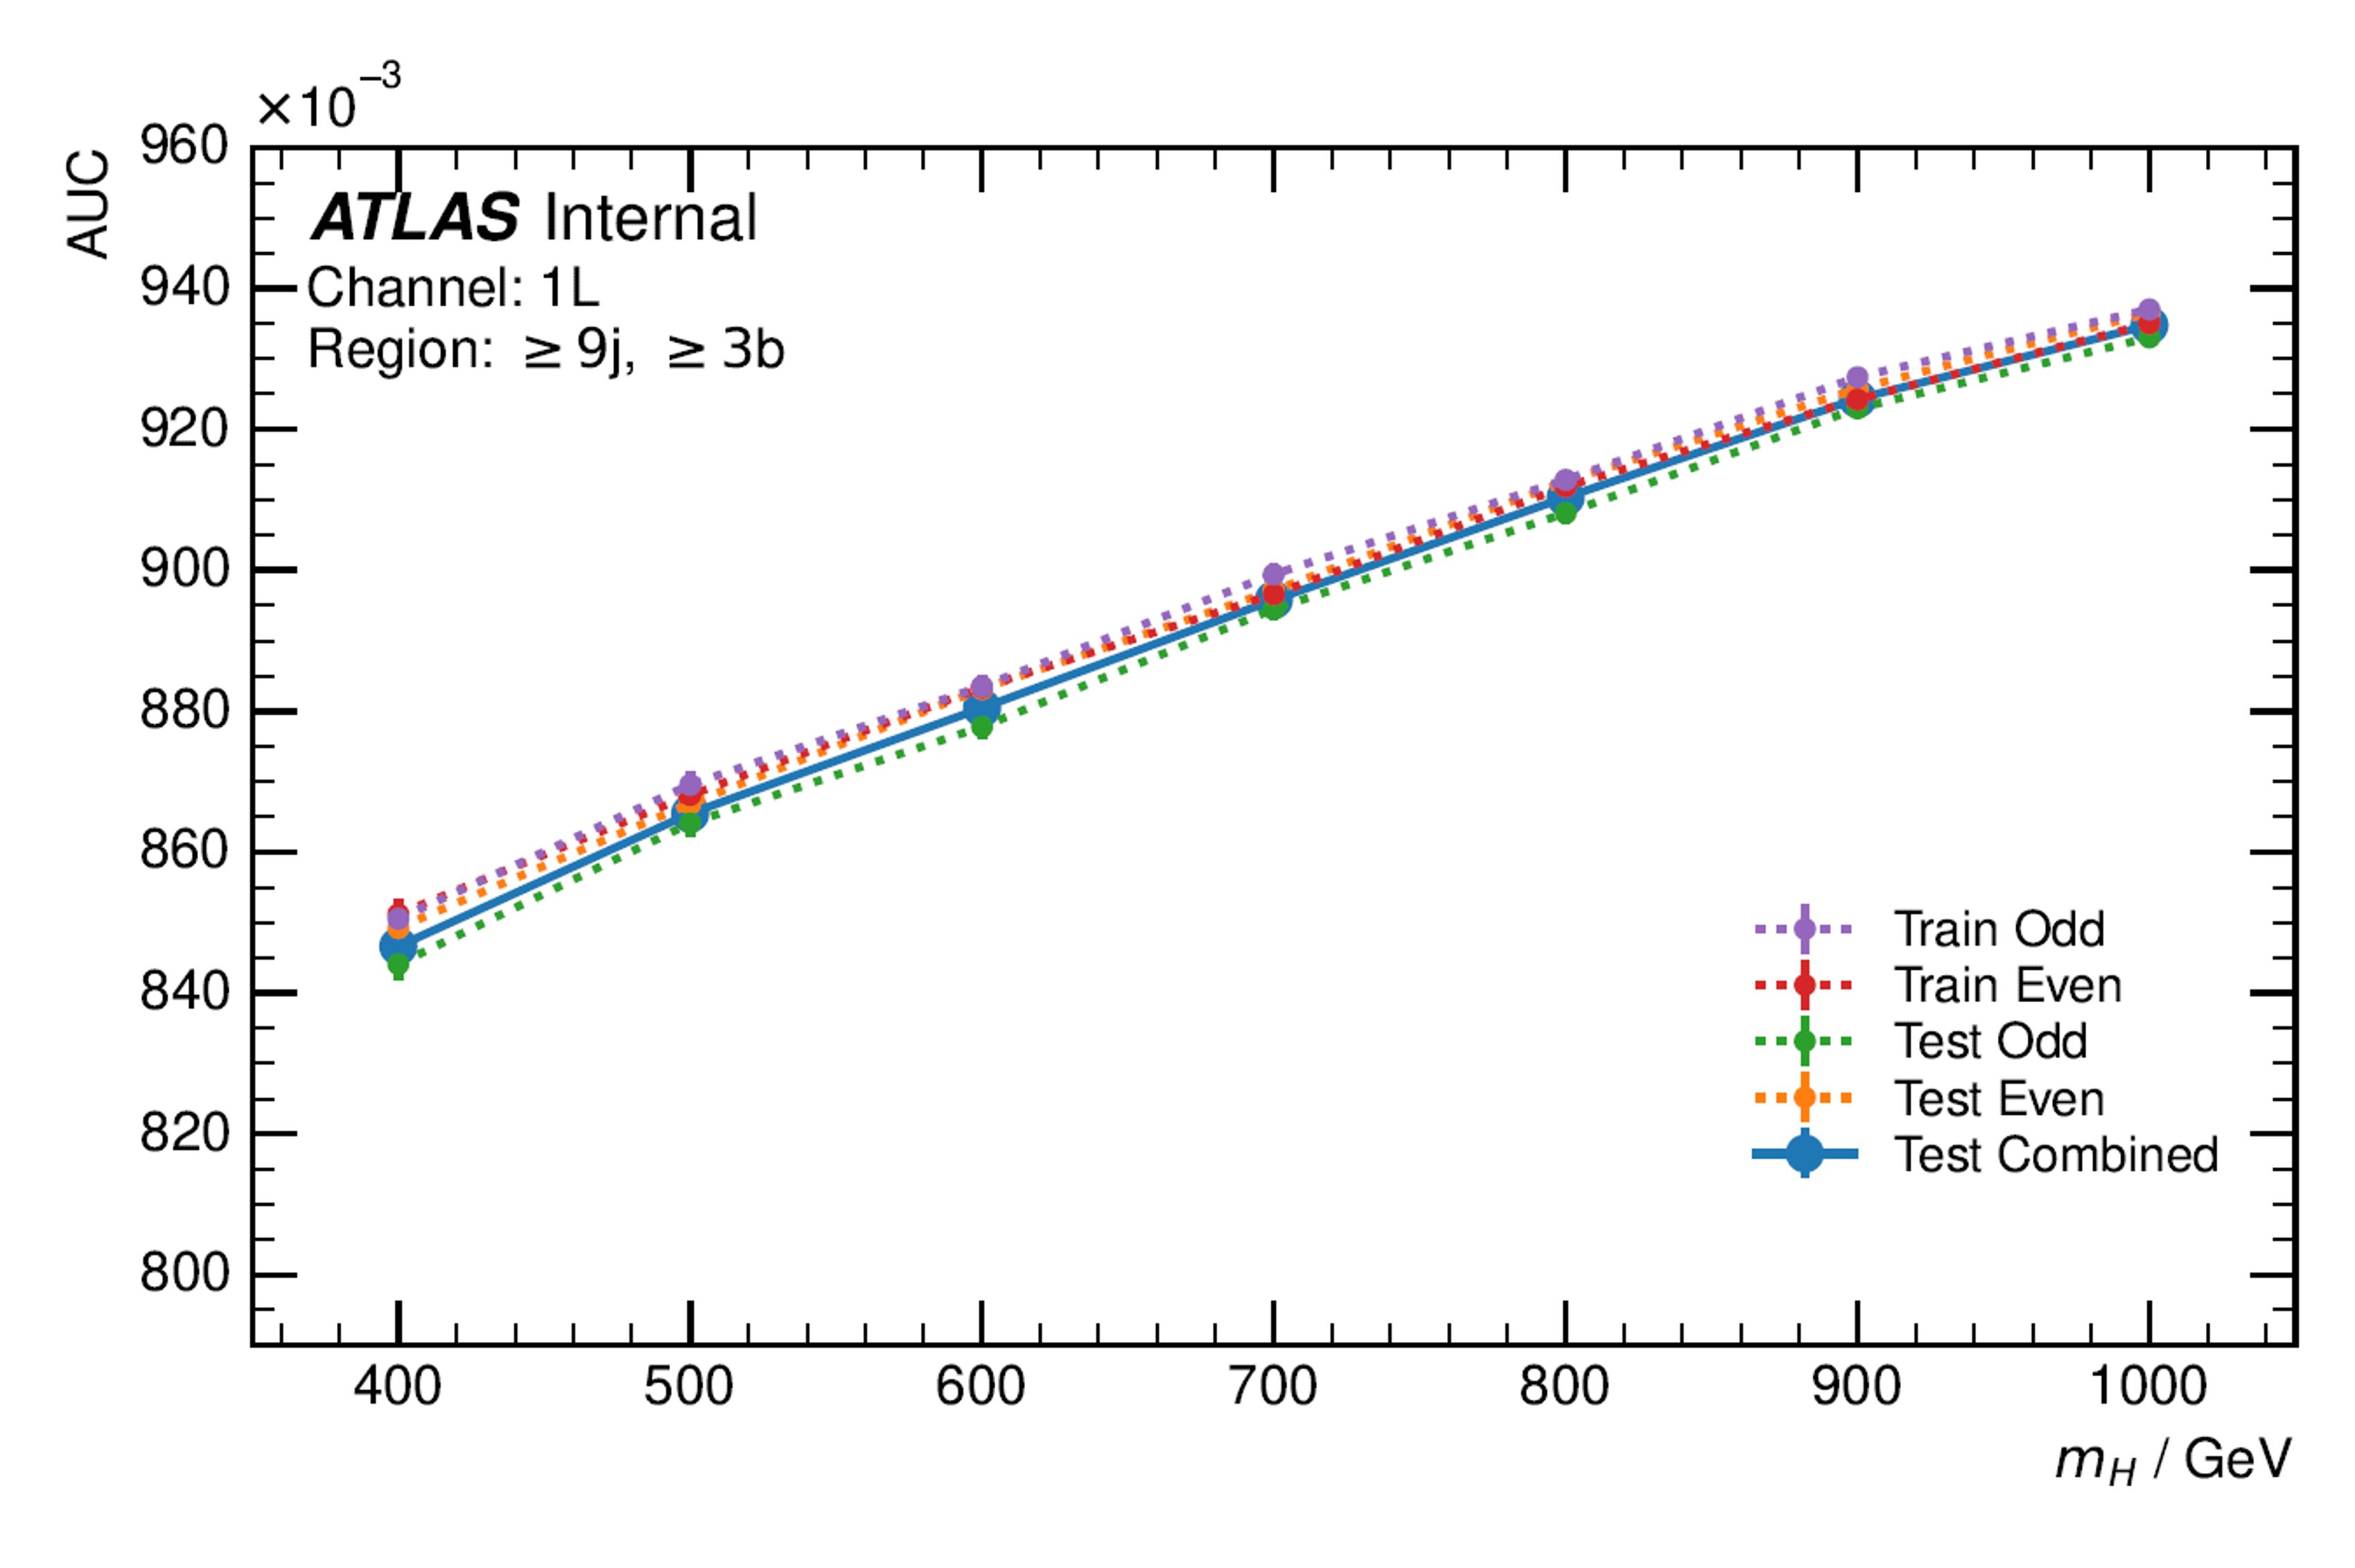
\includegraphics[width=0.48\textwidth]{figures/gnn/Plots_1L/AUC_vs_Mass_Inclusive.png}
        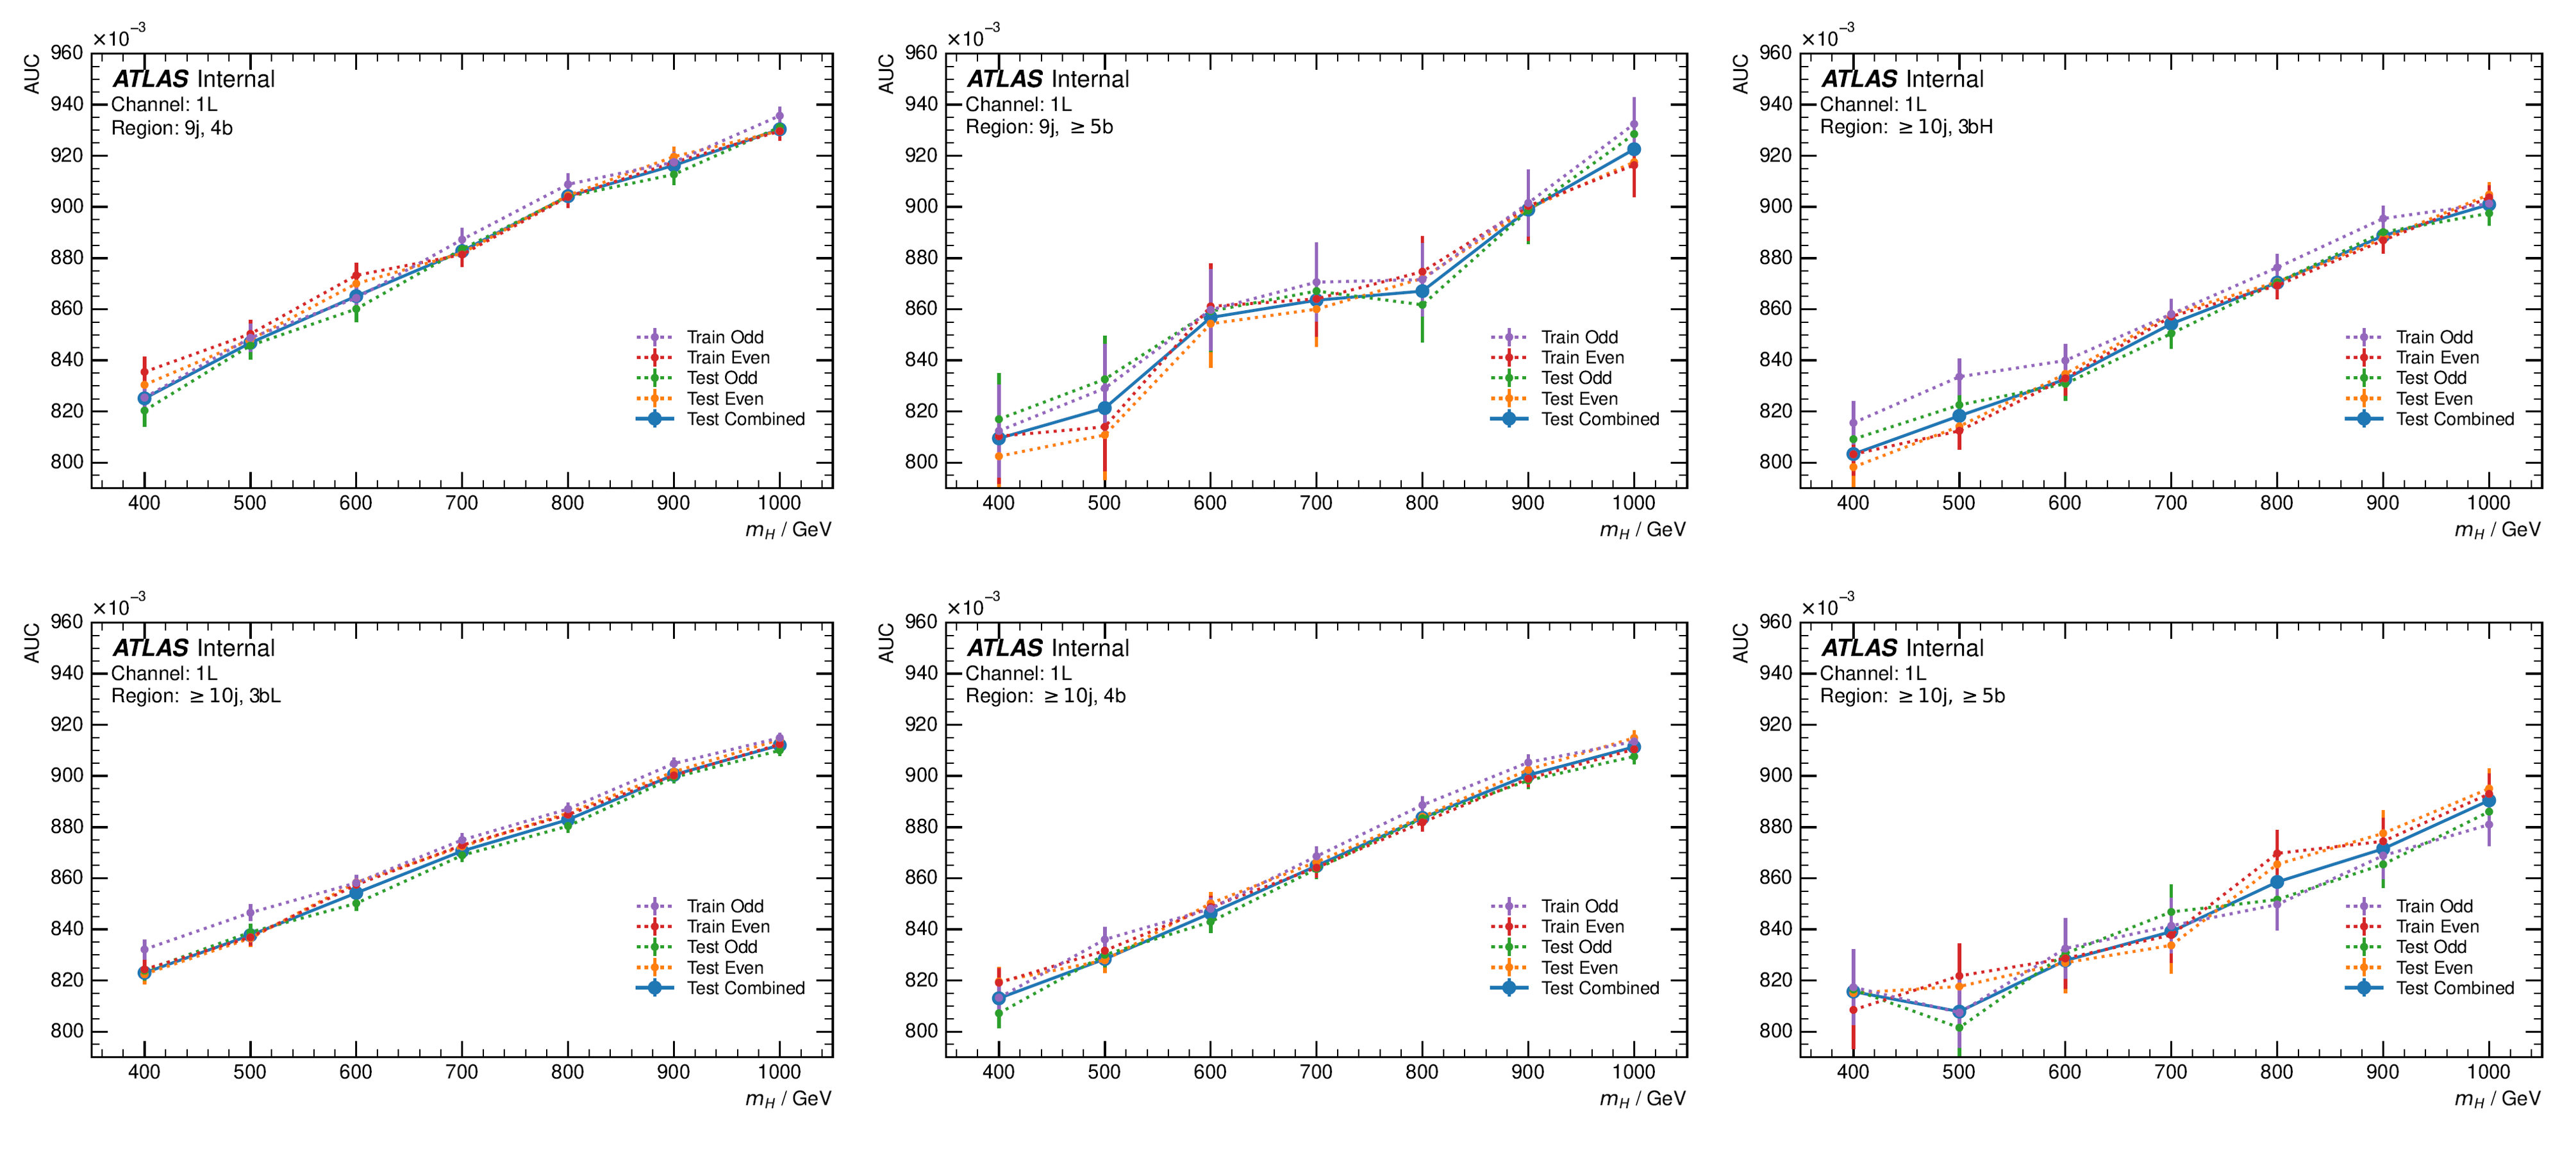
\includegraphics[width=0.48\textwidth]{figures/gnn/Plots_1L/AUC_vs_Mass_Split.png}
        \caption{1L channel}
    \end{subfigure}
    \bigskip
    \centering
    \begin{subfigure}[t]{\textwidth}
        \centering
        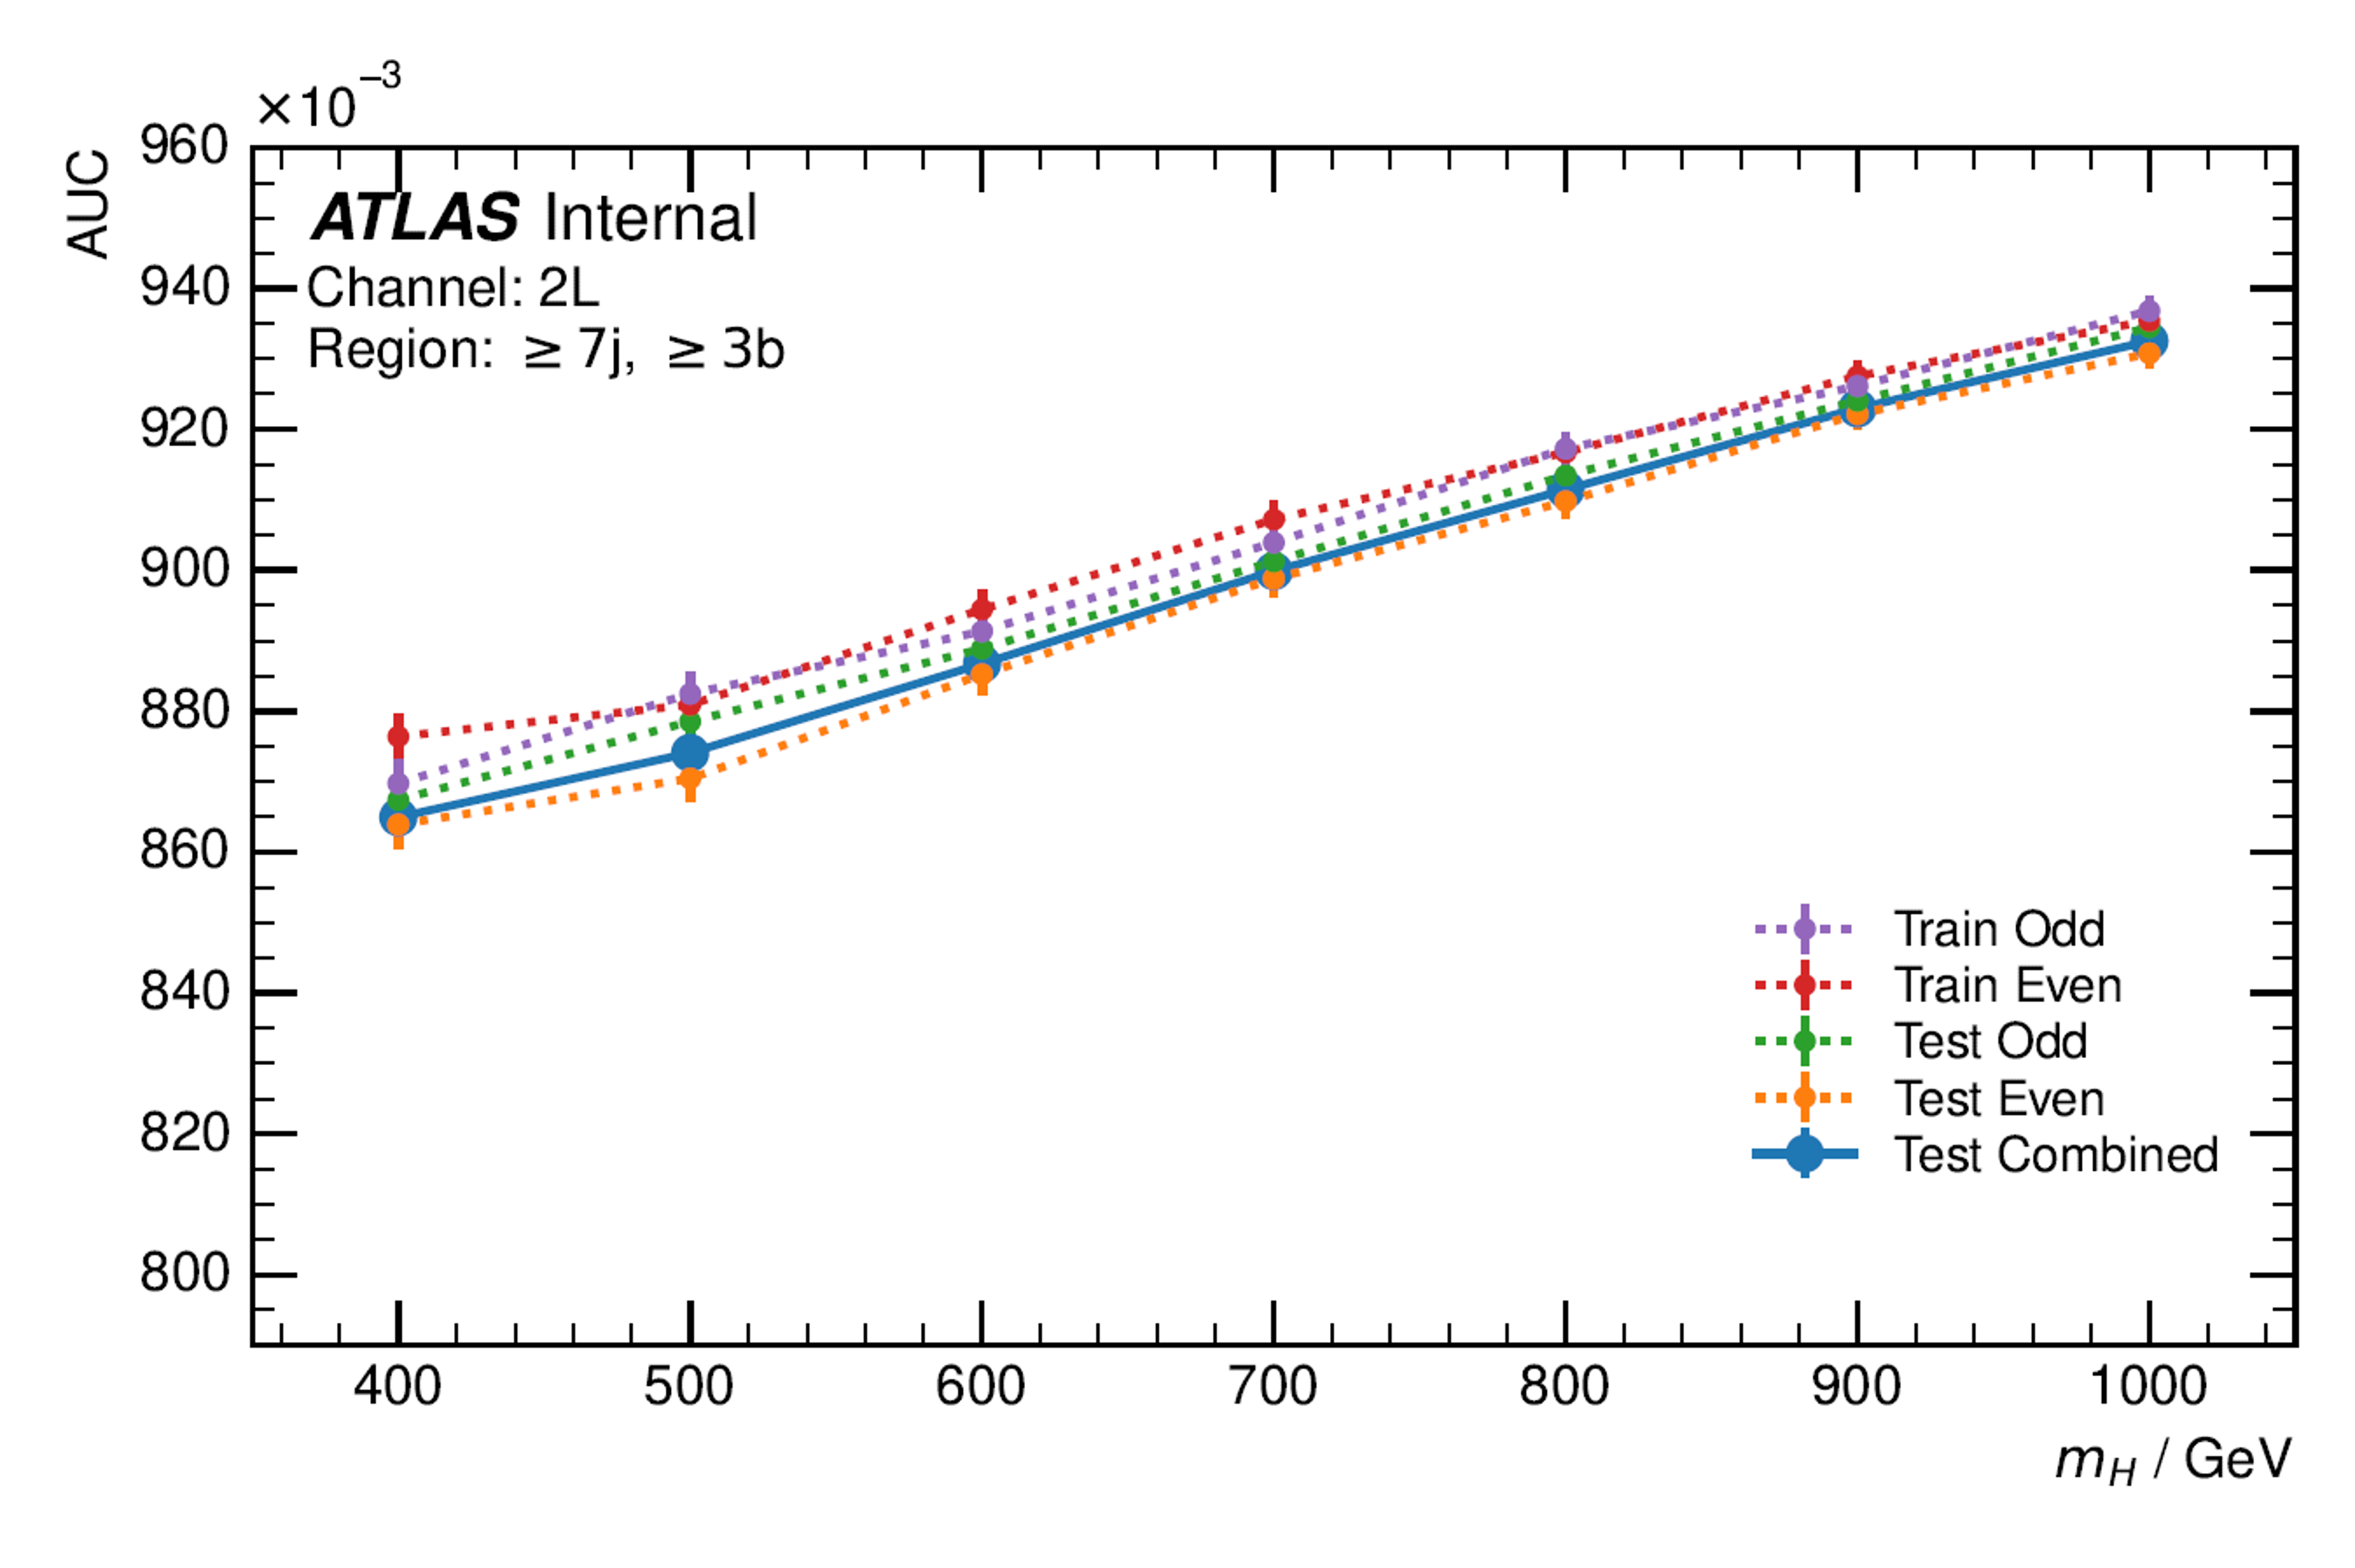
\includegraphics[width=0.48\textwidth]{figures/gnn/Plots_2LOS/AUC_vs_Mass_Inclusive.png}
        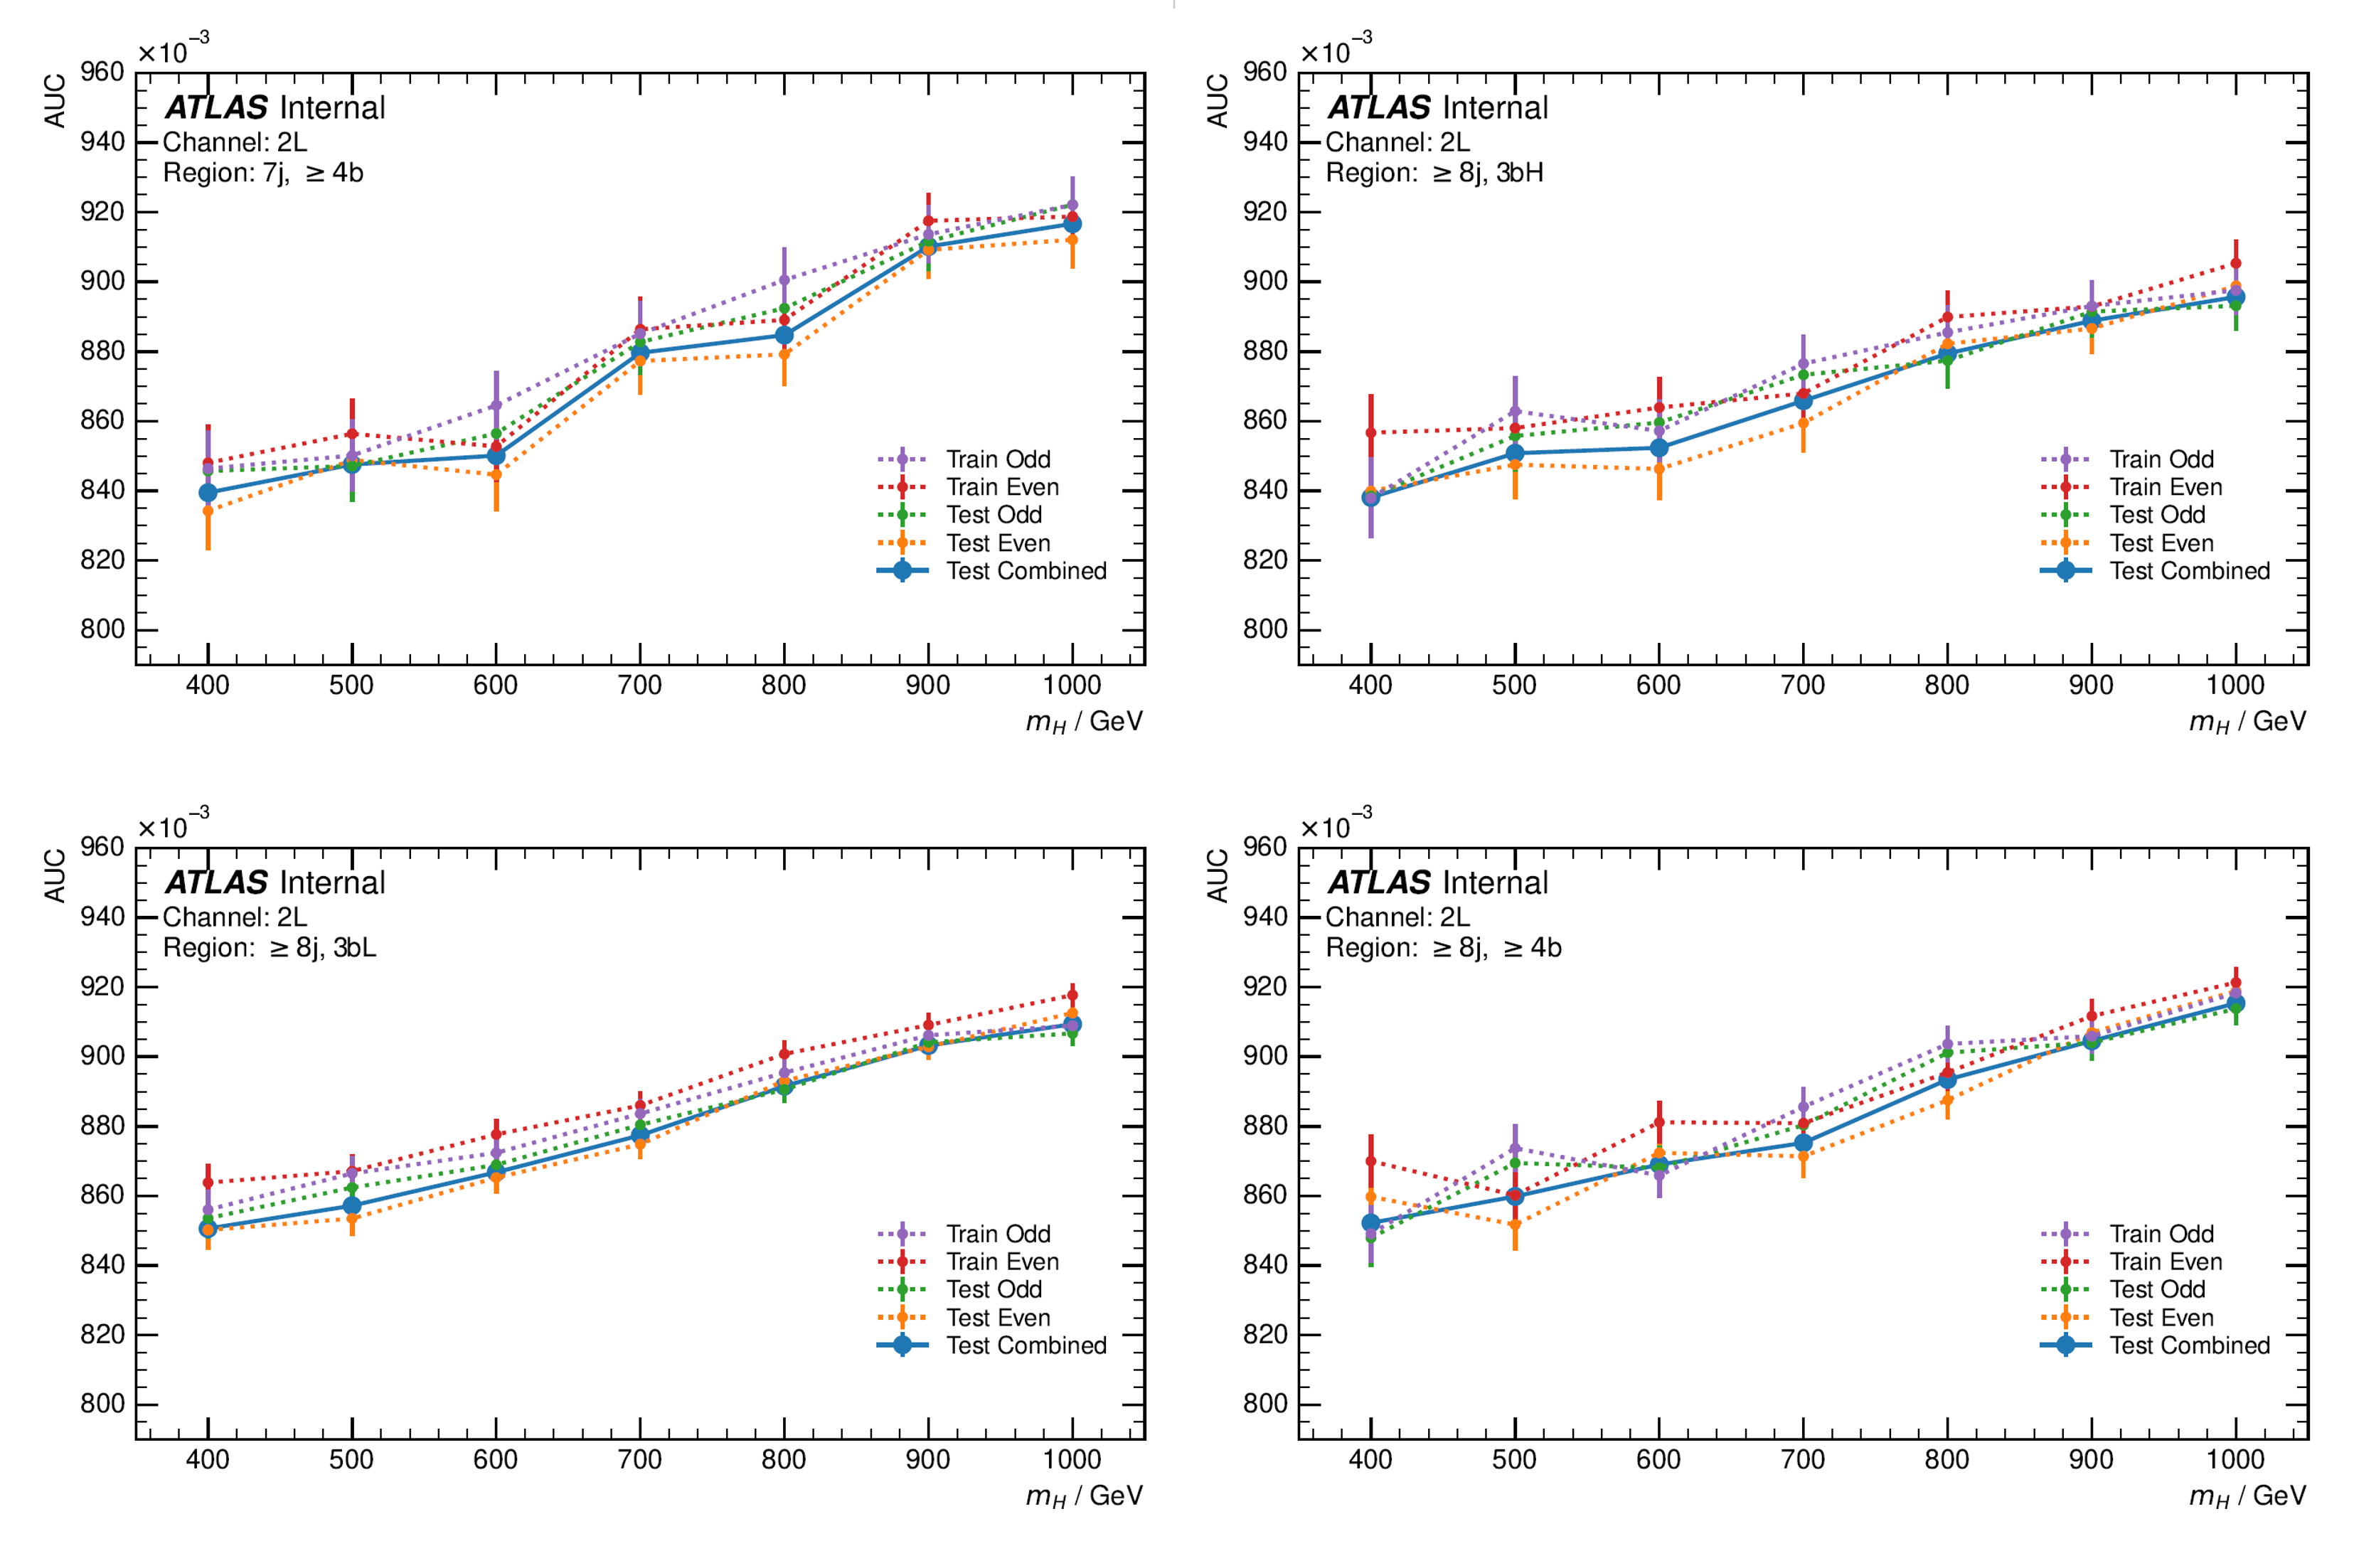
\includegraphics[width=0.48\textwidth]{figures/gnn/Plots_2LOS/AUC_vs_Mass_Split.png}
        \caption{2LOS channel}
    \end{subfigure}
    \caption{Area under ROC curves (AUC) for each mass point for 1L and 2LOS GNN models. Shown in the inclusive training region (left) and four subdivided regions (right). Separate lines are shown for training/testing results of the even/odd event trained models as well as the combined cross-trained model result.}
    \label{fig:AUCvsMass-1LOS}
\end{figure}

\begin{figure}[h!]
    \centering
    \begin{subfigure}[t]{\textwidth}
        \centering
        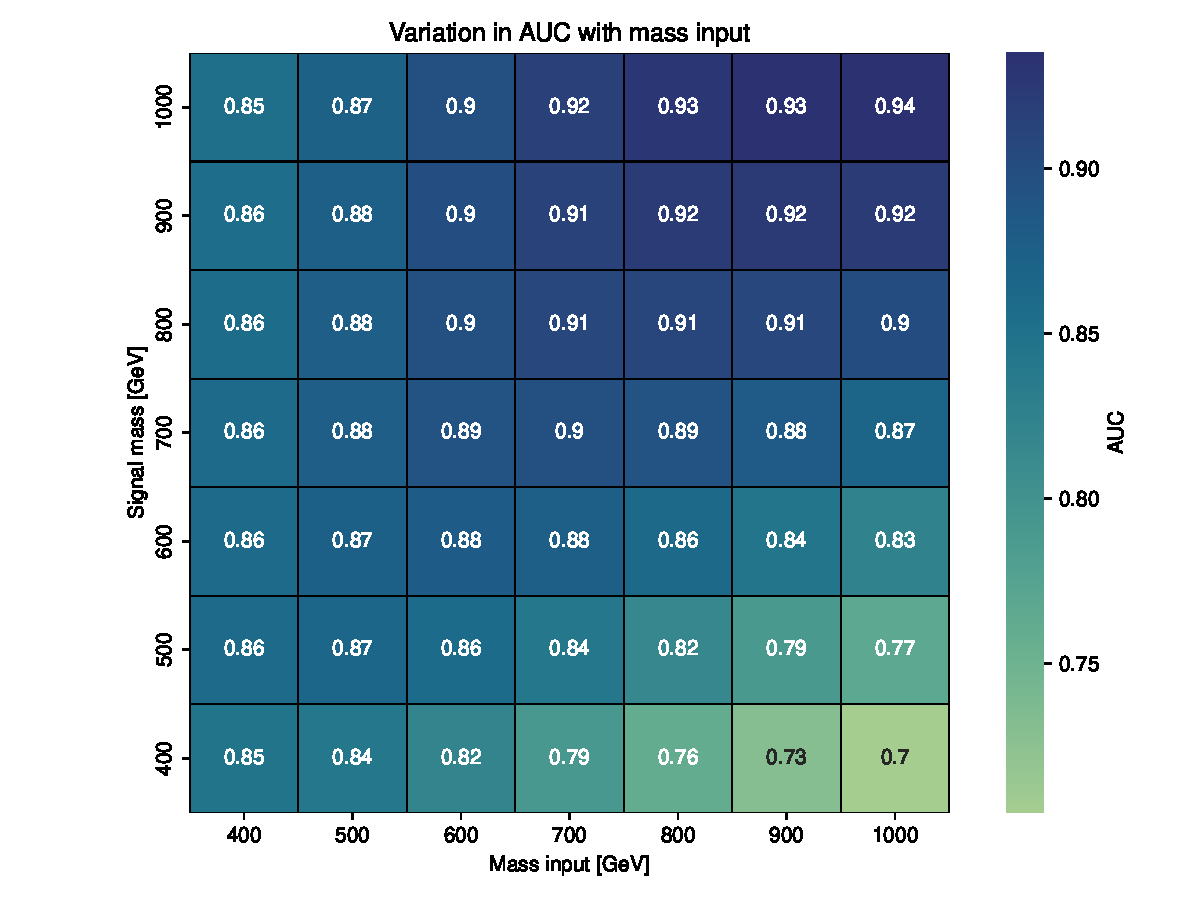
\includegraphics[height=3in]{figures/gnn/Plots_1L/AUC_mass_variations.pdf}
    \caption{1L channel}
    \end{subfigure}
    \bigskip
    \centering
    \begin{subfigure}[t]{\textwidth}
        \centering
        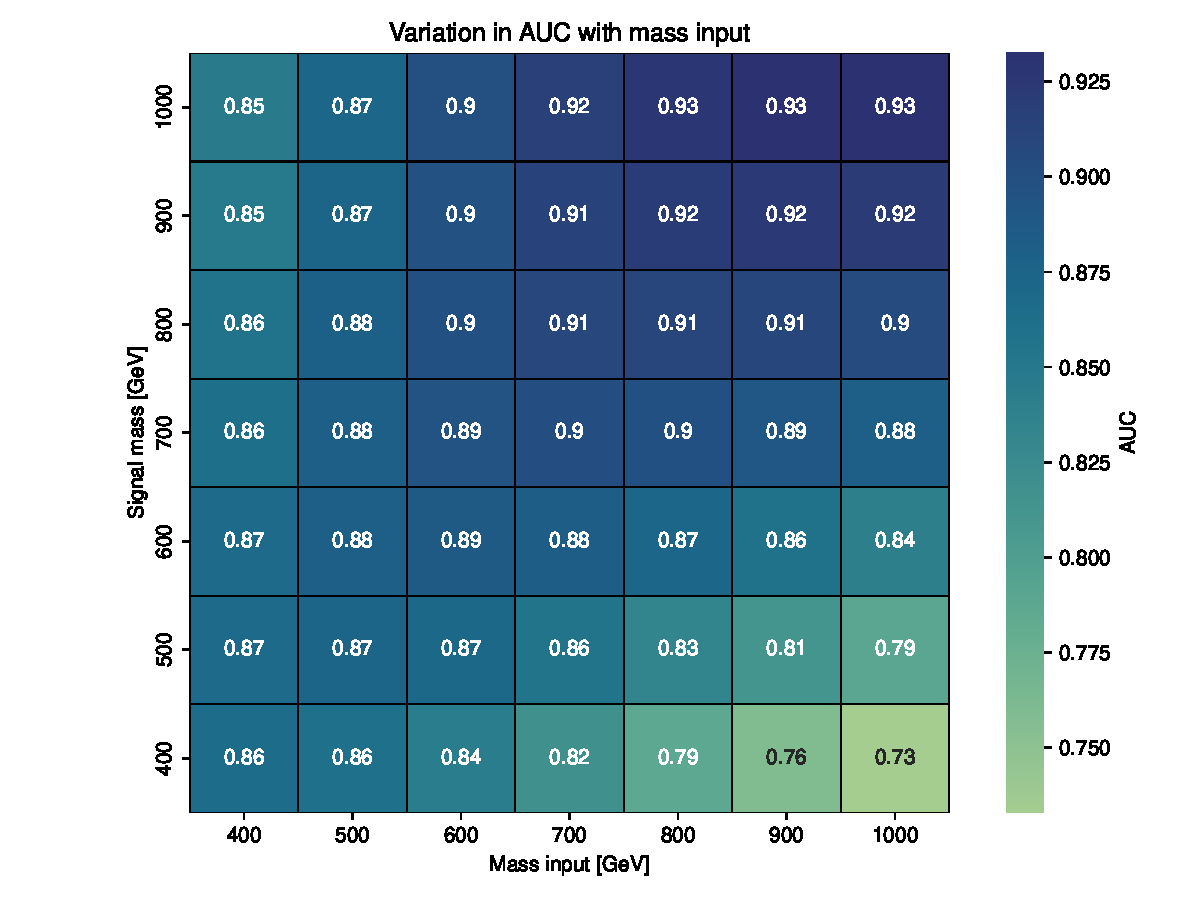
\includegraphics[height=3in]{figures/gnn/Plots_2LOS/AUC_mass_variations.pdf}
    \caption{2LOS channel}
    \end{subfigure}
    \caption{AUC as a function of pseudomass (x-axis) and various signal samples (y-axis).}
    \label{fig:gnn-AUC-mass}
\end{figure}


After training the importance of each input feature is evaluated. The importance of each feature is here defined as the change in loss when a feature in the graph is randomised. The randomisation is performed by shuffling graph features between events in the data set. The feature ranking plots are shown for both channels in figure \ref{fig:gnn-feature-ranking}. The ranking is performed using the inclusive training data set.

\begin{figure}[h!]
    \centering
    \begin{subfigure}[t]{\textwidth}
        \centering
        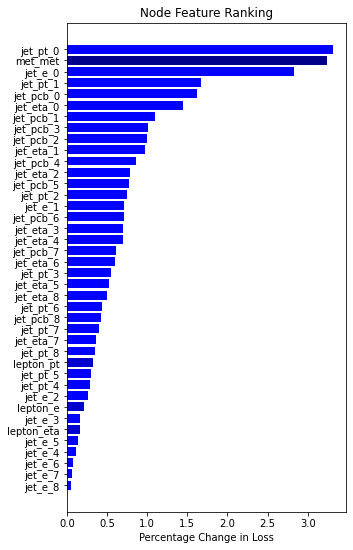
\includegraphics[height=3in]{figures/gnn/Plots_1L/NodeRanking_1L.png}
        \hskip0.3in
        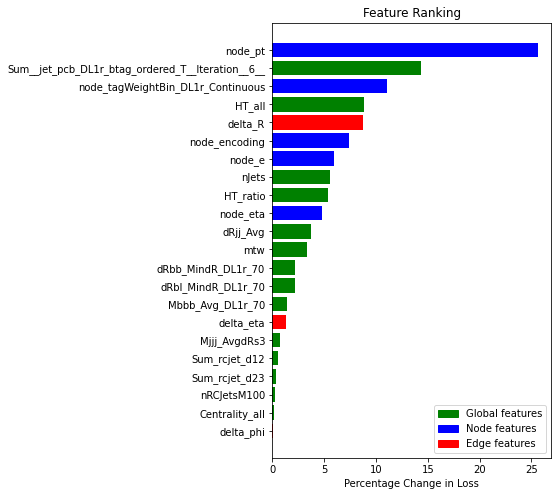
\includegraphics[height=3in]{figures/gnn/Plots_1L/FeatureRanking_1L.png}
    \caption{1L channel}
    \end{subfigure}
    \bigskip
    \centering
    \begin{subfigure}[t]{\textwidth}
        \centering
        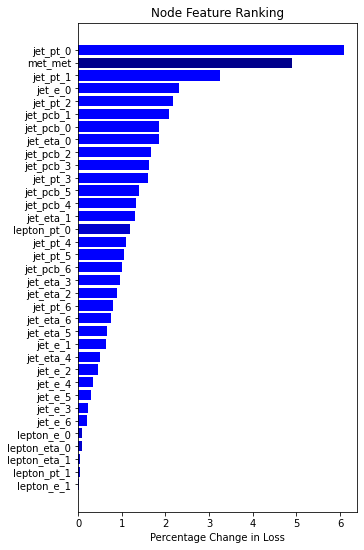
\includegraphics[height=3in]{figures/gnn/Plots_2LOS/NodeRanking_2LOS.png}
         \hskip0.3in
        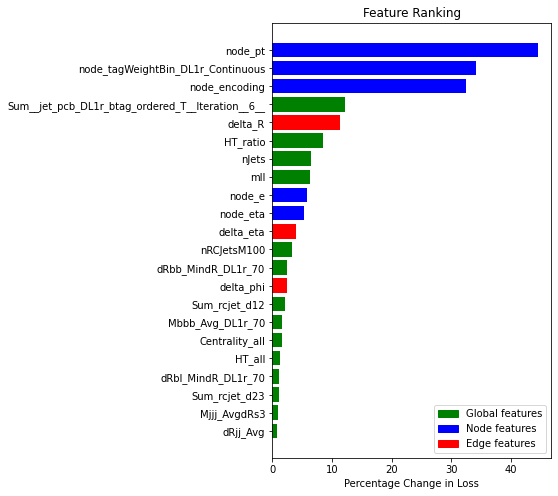
\includegraphics[height=3in]{figures/gnn/Plots_2LOS/FeatureRanking_2LOS.png}
    \caption{2LOS channel}
    \end{subfigure}
    \caption{Feature ranking of the GNN input variables. The feature ranking plot (right) includes all graph features and node/edge features are randomised inclusively of all nodes/edges in the graph. In the node feature ranking plot (left) node features are shuffled on a per object basis.}
    \label{fig:gnn-feature-ranking}
\end{figure}



%-------------------------------------------------------------------------------          


%-------------------------------------------------------------------------------                                                                                                
\FloatBarrier
\section{Systematic uncertainties}% Daniela, Nicola
\label{sec:systematics}
%
Systematic uncertainties arise from the reconstruction of the various physics objects and from theoretical and/or modelling uncertainties affecting the predictions for both the backgrounds and signals. These uncertainties manifest themselves as uncertainties both in the overall yield and shape of the final observable. They are described in this section.

\subsection{Experimental}

A summary of the experimental systematic uncertainties taken into account in this analysis is given in Table~\ref{tab:syst_summary_sources}, along with the shorthand name of the uncertainty used throughout the analysis. 


\subsubsection{Luminosity}

The uncertainty on the integrated luminosity of the combined 2015-2018 dataset is 1.7\%~\cite{ATLAS-CONF-2019-021}. It is obtained using the LUCID-2 detector~\cite{Avoni_2018} for the primary luminosity measurements. The  nuisance parameter is labelled as  \texttt{``luminosity''} and it is applied to all simulated samples. 


\subsubsection{Pileup reweighting}

To account for the difference between the pile-up distributions in data and MC simulations, an uncertainty related to the scale factors used to adjust the MC pile-up to the data pile-up profile is applied. 
The nominal scale-factor applied on the data pile-up distribution when performing the reweighting is changed to $1.0/0.99$ or $1.0/1.07$ to derive the up and down systematic variations, with respect to the nominal value of $1.0/1.03$. This systematic is labelled as  \texttt{``Pileup reweighting''}.


\subsubsection{Electrons}

For electrons, the reconstruction, identification, isolation and trigger performances as well as the lepton momentum scale and resolution differ between data and MC simulation. To correct for these differences, scale factors for each are applied. These scale factors were estimated using the tag-and-probe method~\cite{Aad:2019tso}. The associated systematic uncertainties are then propagated to the final distributions used in this analysis.  A total of eight systematic uncertainties are considered. The ones  related to the efficiency of the trigger, reconstruction, identification and isolation are labelled as \texttt{``ATLAS\_EL\_SF\_[TRIGGER,RECO,ID,ISO]''}.  The ones associated to the energy scale and resolution are named as  \texttt{``ATLAS\_EM\_SCALE\_[AFII,ALL]''} and \texttt{``ATLAS\_EM\_RES}, respectively.  While the one associated to the efficiency of the  ECIDS tool is labelled as \texttt{``ATLAS\_EL\_SF\_ChargeID\_Stat''}. 



\subsubsection{Muons}

As for electrons, scale factors are also applied to muons to correct for the differences between data and simulation~\cite{Aad:2020gmm}. The associated systematic uncertainties are then propagated to the final distributions used in the analysis. The ones related to the efficiency correction factors for trigger, track-to-vertex association (TTVA), identification and isolation are labelled as \texttt{``ATLAS\_MU\_SF\_[TRIG,TTVA,ID,ISO]\_[Stat,Syst]''}, where each one of them is split into a statistical and systematic component.  While the uncertainties related to inner detector track smearing, muon spectrometer track smearing, charge-independent scale momentum and two uncertainties for the charge-dependent scale momentum are labelled as \texttt{``ATLAS\_MU\_[ID,MS,SCALE]''} and  \texttt{``ATLAS\_MU\_SAGITTA\_[RHO,RESBIAS]''},   respectively.  




\subsubsection{Small $R$-jets}

Systematic uncertainties on jets come from  JVT, jet energy scale (JES) and jet energy resolution (JER). They are detailed below.

The systematic uncertainty associated with the JVT is obtained by varying the scale factor used to correct the JVT efficiency in simulation up and down within its uncertainties.  The corresponding nuisance parameter is labelled as \texttt{``Jet vertex tagger efficiency''}. 

Uncertainties on JES are grouped as follow: 15 effective nuisance parameters labelled as \texttt{``JES EffectiveNP''} (2 detector-related, 4 modeling related, 3 mixing both aspects, 6 statistical-related), 6 nuisance parameters related to $\eta$ intercalibration labelled as  \texttt{``JES EtaIntercalibration''} (1 modeling-related, 4 non-closure (highE, 2018data, negEta and posEta), 1 statistical-related), 2 nuisance parameters related to the flavour of the jet labelled as \texttt{``JES Flavour [Composition, Response]''},  4 nuisance parameters related to pile-up subtraction labelled as \texttt{``JES Pileup [OffsetMu, OffsetNPV, PtTerm, RhoTopology]''}, 2 nuisance parameters for punch-through effect treatment labelled as  \texttt{``JES PunchThrough [MC16 ,AFII]''}, 1 nuisance parameter  for non-closure for AFII labelled as \texttt{``JES RelativeNonClosure MC16 AFII''}, 1 nuisance parameter  for the single particle response at high  \pT labelled as \texttt{``JES SingleParticle HighPt''}, and 1 for the $b$-jet response labelled \texttt{`` BJETS\_Response''}.

For the JER a total of 9 independent nuisance parameters are used: 7 effective nuisance parameters labelled as  \texttt{``JER EffectiveNP''}, and 2 additional parameters labelled as  \texttt{``JER DataVsMC [MC16, ALL]''} accounting for the  difference between data and simulation.

\subsubsection{b-tagging}
\label{b-tagging_uncertianties}

In order to calibrate the b-tagging performance, scale factors are applied to the MC events so that the heavy flavour tagging efficiencies are matched with the data. These factors are derived based on the tagging efficiency of b-jets and the mis-tagging rates of c- and light-jets, in bins of the PCB scores, with corresponding uncertainties from each jet flavour. The nuisance parameters correspond to the independent eigenvectors after diagonalizing the covariance matrix from the input systematic uncertainties during the b-tagging calibration. There are a total of 45 nuisance parameters [0-44] describing the real b-jet identification efficiency uncertainties, 20 nuisance parameters [0-19] for c-jets mis-tagging rates uncertainties, and 20 nuisance parameters [0-19] for light-jets mis-tagging rates uncertainties. Additionally, in the context of high-pT extrapolation, further uncertainties are considered as per the new recommended CDI file. These include uncertainties from 5 EV for b-jets, 2 EV for c-jets, and 5 EV for light jets, specifically addressing the high-pT extrapolation uncertainty, above the certain threshold for each flavor~\cite{high_pt_extrapolation,btagging_rec_2023}.



\subsubsection{Missing transverse energy}

The  \MET uncertainty arises due to a possible miscalibration of its soft-track component, and it is estimated from data-MC comparisons of the \pT balance between the hard and soft \MET components. This uncertainty  is modelled by three independent nuisance parameters. They are labelled as  \texttt{``ATLAS\_MET\_SoftScale''}, and  \texttt{``ATLAS\_MET\_SoftRes[Perp,Para]''}.



\begin{table}[h]
  \centering
  \scriptsize
  \begin{center}
    \begin{tabular}{ll}
      \toprule \midrule
      Systematic uncertainty        & Short description                                                                          \\ \midrule
      \multicolumn{2}{c}{\textbf{Event}}  \\ \midrule
      Luminosity  & uncertainty on the total integrated luminosity  \\
       \midrule
       PRW\_DATASF         & uncertainty on data SF used for the computation of pileup reweighting      \\
       \midrule
       \multicolumn{2}{c}{\textbf{Electrons}}  \\ \midrule
       EL\_EFF\_Trigger   & trigger efficiency uncertainty    \\
       EL\_EFF\_Reco    & reconstruction efficiency uncertainty          \\ 
       EL\_EFF\_ID    & ID efficiency uncertainty               \\ 
       EL\_EFF\_Iso   & isolation efficiency uncertainty       \\
       EG\_SCALE\_ALL & energy scale uncertainty  \\ 
       EG\_RESOLUTION\_ALL & energy resolution uncertainty  \\ \midrule
       \multicolumn{2}{c}{\textbf{Muons}}  \\ \midrule
       MUON\_EFF\_Trigger\_STAT        & \multirow{ 2}{*}{trigger efficiency uncertainty}        \\ % todo: guess that includes the ID uncertainty? PR.
       MUON\_EFF\_Trigger\_SYS        &        \\ 
       MUON\_EFF\_ID\_STAT        & \multirow{ 2}{*}{reconstruction uncertainty for \pt > 15 GeV}        \\ % todo: guess that includes the ID uncertainty? PR.
       MUON\_EFF\_ID\_SYS        &        \\ 
       %MUON\_EFF\_ID\_STAT\_LOWPT        & \multirow{ 2}{*}{reconstruction and ID efficiency uncertainty for \pt < 15 GeV}        \\ 
       %MUON\_EFF\_ID\_SYS \_LOWPT       &        \\ 
       MUON\_ISO\_STAT        & \multirow{ 2}{*}{isolation efficiency uncertainty}        \\ 
       MUON\_ISO\_SYS        &        \\ 
       MUON\_TTVA\_STAT        & \multirow{ 2}{*}{track-to-vertex association efficiency uncertainty}        \\ 
       MUON\_TTVA\_SYS        &        \\ 
       MUONS\_SCALE        & energy scale uncertainty                                                           \\ 
       MUONS\_SAGITTA\_RHO        & variations in the scale of the momentum (charge dependent)                  \\ 
       MUONS\_SAGITTA\_RESBIAS        & variations in the scale of the momentum (charge dependent)              \\ 
       MUONS\_ID        & energy resolution uncertainty from inner detector                              \\ 
       MUONS\_MS & energy resolution uncertainty from muon system  \\ \midrule
       \multicolumn{2}{c}{\textbf{Small-R Jets}}  \\ \midrule
       %JET\_GroupedNP  & energy scale uncertainty split into 3 components              \\ 
       %JET\_SR1\_JET\_EtaIntercalibration\_NonClosure & non-closure in the jet response at $2.4<|\eta|<2.5$   \\
       %JET\_SR1\_JER\_SINGLE\_NP  & energy resolution uncertainty  \\
                         JES\_EffectiveNP &  \\
                         JES\_EtaIntercalibration & \\
                         JES\_Flavour &  \\
                         JES\_Pileup &  jet energy scale uncertainties  \\ 
                         JES\_PunchThrough & \\
                         JES\_RelativeNonClosure\_MC16\_AFII & \\
                         JES\_SingleParticle\_HightPt &   \\
                         BJETS\_Response &  \\
                         \midrule
                         JER\_EffectiveNP &  jet energy resolution uncertainties \\
                         JER\_DataVsMC &   \\
                         \midrule
                         JvtEfficiency & JVT efficiency uncertainty  \\
                         
                         %
                         %
                         % todo: decide on b-tagging EV prescription. So far we only have the simplest prescription, but we should switch.
                         %
                         %
                         \midrule
                         FT\_EFF\_EIGEN\_B & $b$-tagging efficiency uncertainties (``SFEigen\_Loose):   \\
                         FT\_EFF\_EIGEN\_C & \\ % \multirow{2}{*}{3 components for $b$-jets, 4 for $c$-jets and 5 for light jets} \\
                         FT\_EFF\_EIGEN\_L &   \\ 
                         FT\_EFF\_EIGEN\_extrapolation &  $b$-tagging efficiency uncertainty on the extrapolation on high \pt-jets  \\ 
                         FT\_EFF\_EIGEN\_extrapolation\_from\_charm & $b$-tagging efficiency uncertainty on $\tau$-jets   \\ \midrule
                         \multicolumn{2}{c}{\textbf{\MET-Terms}}  \\ \midrule
                         %METTrigStat    & \multirow{2}{*}{trigger efficiency uncertainty} -  \\
                         %METTrigSyst &    \\
                         MET\_SoftTrk\_ResoPerp           & track-based soft term related to transversal resolution uncertainty                  \\ 
                         MET\_SoftTrk\_ResoPara           & track-based soft term related to longitudinal resolution uncertainty                  \\ 
                         MET\_SoftTrk\_Scale                  & track-based soft term related to longitudinal scale uncertainty                          \\ 
                         %MET\_JetTrk\_Scale                   & track MET scale uncertainty due to tracks in jets                                            \\ 
                         \bottomrule
                         \end{tabular}
    \end{center}
  \caption{ Qualitative summary of the experimental systematic uncertainties considered in this analysis.}
  \label{tab:syst_summary_sources}
\end{table}


\subsection{Theory/modelling uncertainties on the signal and backgrounds}

%
%\textcolor{red}{\textit{For signal yield uncertainties, these uncertainties are evaluated in a standard way and should 
%include PDF variations and renormalisation/factorisation scale variations.  There is more information
%provided on the PMG TWiki pages for this.}}
%

This section describes the theoretical/modelling uncertainties for the signal and the irreducible background. They are detailed below.  

\subsubsection{\ttbar modelling uncertainties}

\paragraph{Higher order QCD corrections.} Uncertainties due to missing higher order QCD corrections are estimated by varying separately the renormalization and the factorization scales by a factor 2 and 1/2 in the nominal \powhegs\ + \pythiaeight sample. This leads to 6 independent nuisance parameters (2 variations for each of the 3 flavour component, TTL, TTC and TTB).

\paragraph{Matrix-element calculation.} The uncertainty related to the choice of the matrix element (ME) generator is estimated by comparing the predictions of \powhegs and \mgamc. It is expressed in 12 independent nuisance parameters: two variations corresponding to shape and acceptance for each of the 6 flavour sub-processes (\ttl, \ttcin, \ttbb, \ttB, \ttb, \ttbbb). Note that this uncertainty turned out to go beyond the algorithmic ME-PS matching ambiguity as was stated in many previous ATLAS publications. The recent study ~\cite{ATL-PHYS-PUB-2020-023} showed that it convolutes ME-PS matching uncertainty with the matrix element corrections for the parton shower in \powhegs + \pythiaeight but not in \mgamc + \pythiaeight. Thus this uncertainty is just a comparison of two different MC setups rather than ME-PS matching uncertainty.

\paragraph{Parton-shower modelling.} The uncertainty related to the parton shower (PS) and hadronization model is  estimated by comparing the predictions of \powhegs matched with \pythiaeight and \herwigseven. This leads to 12 independent nuisance parameters: two variations corresponding to shape and acceptance for each of the 6 flavour sub-processes (\ttl, \ttcin, \ttbb, \ttB, \ttb, \ttbbb).

\paragraph{Radiations modelling.} The uncertainty on the amount of initial state radiations (ISR) predicted by the PS generator is estimated by varying the value of the strong coupling \alphas{} at the scale of the $Z$-boson mass around its tuned value in A14\footnote{The A14 tuned variations of ${\alphas}^{ISR}(M_Z)$ is usually referred as Var3c and numerically corresponds to ${\alphas}^{ISR}(M_Z)=0.127^{+0.013}_{-0.012}$~\cite{ATL-PHYS-PUB-2014-021}} in the ISR model of \pythiaeight. The uncertainty on the amount of finial state radiations (FSR) predicted by the PS generator is estimated by varying the factorization scale by a factor $2$ and $1/2$ in the FSR model of \pythiaeight. The uncertainty coming from the choice of the \hdamp{} value is estimated by comparing the predictions between $\hdamp=1.5\,\mtop$ and $3\,\mtop$. This leads to $9$ independent nuisance parameters ($3$ variations for $3$ flavour sub-processes).

\paragraph{Normalization of \ttbar subsamples} A flat uncertainty of $50\%$ is applied to the normalisation of the \ttbin and \ttcin contributions separately to correct any mis-modelling related to the \ttbar production in association with extra heavy-flavor jets. This leads to $2$ nuisance parameters. A flat uncertainty of $5\%$ is applied to the normalisation of the \ttl. Two nuisance parameters are used for that: one acting in the 1L regions and the second acting in the 2L regions.

\paragraph{4v5FS comparison.} A comparison of the \ttbin\ simulation by the nominal \ttbar\ sample based on the 5F scheme with the best theoretical NLO prediction using 4F scheme implemented in the \powhegboxRes generator (see Sect.~\ref{sec:samples} for the details of the setup) showed large difference between these two predictions in the phase space of the analysis. Therefore, an additional uncertainty is expressed in 8 independent nuisance parameters: two variations corresponding to shape and acceptance for each of the 4 flavour sub-processes (\ttbb, \ttB, \ttb, \ttbbb), where we compare these two schemes.

\paragraph{NN reweighting} Additional three nuisance parameters are used for all \ttbar subprocesses (correlated among the subprocesses) due to NN reweighitng uncertainties as explained in Section \ref{sec:NN_reweighting:uncertainty}.

All the red/blue plots for the main systematic variations for sample \ttbin can be found in Appendix~\ref{app:TTB_modeling}.


\subsubsection{Other uncertainties}

\begin{description}
\item[Signal:]  Renormalisation and factorisation scale variations are used as systematics for the signal.  The uncertainty is labelled as \texttt{``signal varRF''} and it is estimated by varying the renormalisation and the factorisation scales together by a factor 2 and $1/2$ in MadGraph5\_aMC@NLO. An additional PDF uncertainty of 1\% labelled as \texttt{``signal PDF''} is also applied. 

\item[$\tttt$:] The modelling uncertainties on the \tttt signal are estimated by applying the generic theoretical uncertainties from the MC simulation.
The uncertainty related to the parton shower and hadronization model is labelled as ``\texttt{tttt modelling (shower)}` and is estimated by comparing the predictions between \mgamc matched with \pythiaeight and \mgamc matched with \herwigseven.
The uncertainty related to the ME generator is labelled as ``\texttt{tttt varRF}`` and is estimated by varying the renormalization and the factorization scale together by a factor $2$ and $1/2$ in \mgamc.
Finally, an additional cross-section uncertainty labelled a ``\texttt{tttt cross-section}`` is applied. Its upper size is +7.8\% and its lower size is -13.3\% based on Ref.~\cite{vanBeekveld:2022hty}.


\item[$\ttW$, $\ttZ$, and $t\bar tH$:] Modelling uncertainties for these processes are evaluated in a similar way. Uncertainties associated to the generator are labelled \texttt{``[ttW,ttZ,ttH] modelling (generator)''}. They are estimated by comparing the predictions from the nominal generator with an alternative one. For $\ttW$, the \sherpa 2.2.10 sample is compared to MadGraph5\_aMC@NLO+Pythia8. For $\ttZ$, the \sherpa 2.2.1 sample  is compared to MadGraph5\_aMC@NLO+Pythia8, while for $t\bar tH$  Powheg is compared to MadGraph5\_aMC@NLO+Pythia8. Uncertainties associated to the renormalisation and factorisation scale variations are labelled as \texttt{``[ttW,ttZ,ttH]\_varRF''} and are computed in the same way as for the signal.

  Additional uncertainty on the production in association with additional jets is applied by considering an uncertainty of 10\%, 20\% and 30\% for events with respectively 9 (7), 10 (8) and at least 11 (9) jets  in the 1L (OS) channel.
These values of uncertainty are based from the level of \ttjets \Nj mismodelling observed in the 2$b$ region before reweighting.
An uncertainty of $12\%$ and $10\%$ is respectively applied on the \ttZ and \ttH total cross-section and is labelled as ``\texttt{[ttZ,ttH] Cross-Section}``.

\item[Single top:]  The single top production includes the t-channel, tW-channel and s-channel production mode.
The modelling uncertainty is estimated by comparing the prediction from different matrix element (\powhegs vs \mgamc) and parton shower (\pythiaeight vs \herwigseven) generator, by comparing different \ttbar and single top interference scheme (diagram removal vs diagram subtraction) and by varying both the renormalization and the factorization scales by a factor $2$ and $1/2$.
A total uncertainty of $30\%$ is applied on this background.
The associated nuisance parameter is labelled as ``\texttt{singleTop Cross-Section}``.

\item[Minor processes:] An uncertainty of 60\% is applied on \Vjets based on Ref~\cite{Alwall:2007fs}.
For all the other minor background processes, an ad-hoc uncertainty of $50\%$ is applied on their total cross-section.


\end{description}




%-------------------------------------------------------------------------------          


%-------------------------------------------------------------------------------                                                                                                
\FloatBarrier
\section{Statistical analysis}% Daniela, Nicola
\label{sec:stats}
%
The MVA discriminant distributions from each of the regions considered are combined to test for the presence of a signal.
%Ten bins are used in the 2bex and 3bex regions, while only a single bin in the $\geq$4b regions. 
The statistical analysis is based on a binned likelihood function ${\cal L}(\mu,\theta)$ constructed as
a product of Poisson probability terms over all bins considered in the analysis:

\begin{eqnarray}
    L\left(\vec{n}|\mu, \vec{\theta}\right) = \prod_{r \in \text{region}}\prod_{i\in \text{bin}} \text{Pois}\left(n_{i,r}|\mu S_{i,r}(\vec{\theta}) + B_{i,r}(\vec{\theta})\right)\times\prod_{j\in \text{NP}}G\left(\theta_j\right),
\label{eq:Likelihood}
\end{eqnarray}

\noindent where $\vec{n}$ represents the data vector, with $n_{i,r}$ representing data yields in the bin $i$ and region $r$.
$\vec{\theta}$ denotes the NPs, that affect the number of signal events $S_{i,r}$ as well as the number of background events $B_{i,r}$ in the bin $i$ and region $r$. Finally, $\mu$ is the signal strength, which is the parameter of interest in the likelihood and it represents the ratio of the measured over reference cross section $\sigma_{4t}^{BSM}=12$ fb$^{-1}$). The terms, Pois and $G$, represent the Poisson and Gaussian distributions, respectively. It is clear from Eq.~\ref{eq:Likelihood} that the NPs are constrained by the Gaussian term\footnote{For the \emph{gamma} terms, representing the MC statistical uncertainty, the constraint term is Poisson --- in Bayesian statistics this would result in Gamma function posterior distribution, hence the name.} while the normalisation parameters, $\vec{k}$ are unconstrained. The full form of the likelihood can be found in the \emph{HistFactory} reference~\cite{Cranmer:1456844}.

The total number of expected events in a given bin depends on $\mu$ and
$\theta$. The nuisance parameters $\theta$ adjust the expectations for signal and background
according to the corresponding systematic uncertainties, and their fitted values correspond to the deviations from
the nominal expectations that globally provide the best fit to the data.
This procedure allows a reduction of the impact of systematic uncertainties on 
the search sensitivity by taking advantage of the highly populated background-dominated channels included in the likelihood fit.
It requires a good understanding of the systematic effects affecting the shapes of the discriminant distributions.
Detailed validation studies of the fitting procedure have been performed using the simulation.
To verify the improved background prediction, fits are performed under the background-only hypothesis.
Differences between the data and the background prediction are also checked relative to the smaller post-fit uncertainties
in kinematic variables other than the ones used in the fit.
Statistical uncertainties in each bin of the discriminant distributions are also taken into account by dedicated parameters in the fit, referred to as ``$\gamma$ factors".
In order to speed up the fit, systematic uncertainties that have very a small effect on normalisation or shape are pruned, per process and analysis channel. 
The pruning algorithm removes systematic uncertainties that have a $\leq$0.5\% impact on normalisation or those that cause
a negligibly small impact on the shape of the final discriminant (all bins are within 0.5\% of the nominal shape).

The test statistic $q(\mu)$ is defined as the profile likelihood ratio: 
$q(\mu) = -2\ln({\cal L}(\mu,\hat{\hat{\theta}}_\mu)/{\cal L}(\hat{\mu},\hat{\theta}))$,
where $\hat{\mu}$ and $\hat{\theta}$ are the values of the parameters that
maximise the likelihood function (with the constraint $0\leq \hat{\mu} \leq \mu$), and $\hat{\hat{\theta}}_\mu$ are the values of the
nuisance parameters that maximise the likelihood function for a given value of $\mu$. 
The test statistic $q(\mu)$ is implemented in the {\sc RooFit} package~\cite{Verkerke:2003ir,RooFitManual} and
is used to measure the compatibility of the observed data with the background-only hypothesis (i.e. the discovery test)  
setting $\mu=0$ in the profile likelihood ratio: $q(0) = -2\ln({\cal L}(0,\hat{\hat{\theta}}_0)/{\cal L}(\hat{\mu},\hat{\theta}))$.
The actual statistical analysis package used is {\sc TRexFitter}~\cite{TRexFitterTwiki}, which makes use of the {\sc RooFit} and {\sc RooStats} packages.
The $p$-value (referred to as $p_0$) representing the compatibility of the data with the background-only hypothesis is estimated by integrating
the distribution of $q(0)$ from background-only pseudo-experiments, approximated using the asymptotic formulae given in Refs.~\cite{Cowan:2010js,ErratumCowan:2010js}, 
above the observed value of $q(0)$. Some model dependence exists
in the estimation of the $p_0$-value, as a given signal scenario needs to be assumed in the calculation of the denominator of $q(\mu)$, even 
if the overall signal normalisation is left floating and fitted to data. The observed $p_0$-value is checked for each explored signal scenario.
In the absence of any significant excess above the background expectation, upper limits on $\mu$ for each of the 
signal scenarios considered are derived by using $q(\mu)$ in the CL$_{\rm{s}}$ method~\cite{Junk:1999kv,Read:2002hq}.
For a given signal scenario, values of $\mu$ yielding CL$_{\rm{s}}$<0.05,  
where CL$_{\rm{s}}$ is computed using the asymptotic  approximation~\cite{Cowan:2010js}, are excluded at $\geq$95\% CL.

%a smoothing based on ROOT implementation\footnote{Implementation in ROOT {\tiny{$https://root.cern.ch/doc/v606/TH1\_8cxx\_source.html\#l06440$}}, \\
%usage in TRexFitter {\tiny{$https://gitlab.cern.ch/TRExStats/TRExFitter/blob/master/Root/Common.C\#L444$}}} is applied before an histogram 
%is translated into a likelihood function as needed in cases where the input histograms suffer from large statistical fluctuations; affected samples are V+jets. 

The profile likelihood fit is performed in Signal Regions (SRs) and Control Regions (CRs). The single lepton(dilepton opposite sign) channel includes 6(4) SRs ang 6(5) CRs respectively.  The six signal regions for 1L are 9j4b, 9j$\ge5$b, $\ge10$j3bH, $\ge10$j3bL, $\ge10$j4b, $\ge10$j$\ge5$b while six control regions are 8j3bH, 8j3bL, 8j4b, 8j$\ge5$b, 9j3bH, 9j3bL. Similarly for dilepton opposite sign channel, four signal regions include 7j$\ge4$b, $\ge8$j3bL, $\ge8$j3bH, $\ge8$j$\ge4$b while five control regions include 6j3bH, 6j3bL, 6j$\ge4$b, 7j3bH, 7j3bL.




%Once unblinded, fits are performed to data under the signal-plus-background hypothesis, where the
%signal strength parameter, $\mu$, is the parameter of interest in the fit and is allowed to float freely, 
%but is required to be the same in all fitted regions.  In order to study the expected behavior of the fit,
%fits are also performed to the ``Asimov dataset'', defined as the sum of the total expected background,
%although for some tests (e.g. the calibration of the signal strength parameter $\mu$), simulated 
%signal assuming a given branching ratio can also be included on the Asimov dataset.
%Normalisation of all backgrounds is determined from the fit simultaneously with the
%$\mu$. Contributions from $\ttbar$, $W/Z$+jets production, single 
%top, diboson, $t\bar{t}H$ and $t\bar{t}V$ backgrounds are constrained by the uncertainties 
%of the respective theoretical calculations, the uncertainty in the 
%luminosity, and the data themselves.  Statistical uncertainties in each bin of the discriminant 
%distributions are taken into account by dedicated parameters in the fit. 


\subsection{Blinding strategy}% Daniela, Nicola
\label{sec:blinding}
%
The following blinding procedure is used: in each analysis 
channel, those bins of the MVA (BDT or GNN) discriminant distribution with a signal-to-background ratio ($S/B$) 
greater than 5\% are removed. The procedure applied assuming a given signal at the time to contribute to the corresponding MVA score: for example, when looking at the BDT score evaluated for \mH=500~\gev\ only the presence of a possible signal with \mH=500~\gev\ is accounted for in the blinding procedure. 
The signal is normalised to 12~\ifb that represents the measured four-top-quark cross section from Ref.~\cite{ATLAS-CONF-2021-013} 
minus the expected SM prediction.  

Following this procedure, the number of blinded MVA bins depends marginally on \mH discriminant under consideration; between 8 and 12 bins are blinded overall across all channels for each \mH hypothesis. 

\subsection{Binning strategy}% Daniela, Nicola
\label{sec:binning}
%
The binning of the MVA discriminants is broadly optimised simultaneously for all signals.  
The method is based on the implementation available in the software framework~\cite{TRexFitterTwiki}.  
The main idea is to define the binning in an iterative manner based on the variable

\begin{equation}
Z=Z_{b}\frac{n_{b}}{N_{b}}+Z_{s}\frac{n_{s}}{N_{s}}
\end{equation}
where ``s'' and ``b'' refers to ``signal'' and ``background''.
The two input parameters of the algorithm are $Z_{b}$ and $Z_{s}$, their sum is taken to the total number of bins. In order to define each bin, 
a boundary is obtained from the condition: $Z\geq 1$. The variable $n_{X}$ (X=s,b) is defined as signal or background yields in a single bin
\begin{equation}
n_{X}^{i}==n_{X}=\sum_{i=s,b}n_{X}^{i}
\end{equation}
and $N_{X}$ (X=s,b) is signal and background yields in all bins
\begin{equation}
N_{X}=\sum_{i=1}^{N_{\mathrm{bins}}}n_{X}^{i}
\end{equation}

The algorithm starts from the lowest boundary, integrating signal and background yields to obtain $n_x$ until $Z\geq 1$ is found. 
Then the value when $Z\geq 1$ is firstly found is defined as the upper boundary of the first bin. Then the algorithm iterates to find the next bin edges.
As example, for $Z_{b}=N_{bins}$ and $Z_{s}=0$, the corresponding binning will have $n_{b}=N_{b}$ in each bin, that is the binning will be 
constructed in a way that makes the background flat in the investigated MVA discriminant. 
For this search we use multiple settings of the $Z_{b}$ and $Z_{s}$ parameters depending on the expected fraction of the signal in a give region, a summary 
of the binning setting is given in Tab.~\ref{tab:binning}.  


%%%%%%%%%%
\begin{table}
\begin{center}
\begin{tabular}{|c|c|c|c|c|} 
\hline
1L  &  3bL & 3bH & 4b & $\geq$ 5b\\ 
\hline
8j        &  $Z_{b}$=4,  $Z_{s}$=0, Var=H$_{T}$    &  $Z_{b}$=4,  $Z_{s}$=0, Var=H$_{T}$   &  $Z_{b}$=4,  $Z_{s}$=0, Var=H$_{T}$  & $Z_{b}$=1, $Z_{s}$=0, Var=H$_{T}$ \\
9j        &  $Z_{b}$=4,  $Z_{s}$=0, Var=H$_{T}$    &  $Z_{b}$=4,  $Z_{s}$=0, Var=H$_{T}$   &  $Z_{b}$=3,  $Z_{s}$=1, Var=MVA      &  $Z_{b}$=1,  $Z_{s}$=0, Var=MVA     \\
$\geq$10j &  $Z_{b}$=2,  $Z_{s}$=2, Var=MVA        &  $Z_{b}$=2,  $Z_{s}$=2, Var=MVA      &  $Z_{b}$=2,  $Z_{s}$=2, Var=MVA      &  $Z_{b}$=1,  $Z_{s}$=0, Var=MVA     \\
\hline
\end{tabular}

\begin{tabular}{|c|c|c|c|} 
\hline
2LOS  &  3bL & 3bH & $\geq$ 4b \\ 
\hline
6j        &  $Z_{b}$=3,  $Z_{s}$=0, Var=H$_{T}$     &  $Z_{b}$=3,  $Z_{s}$=0, Var=H$_{T}$   &  $Z_{b}$=3,  $Z_{s}$=0, Var=H$_{T}$  \\
7j        &  $Z_{b}$=3,  $Z_{s}$=0, Var=H$_{T}$     &  $Z_{b}$=3,  $Z_{s}$=0, Var=H$_{T}$   &  $Z_{b}$=2,  $Z_{s}$=2, Var=MVA      \\
$\geq$8j  &  $Z_{b}$=2,  $Z_{s}$=2, Var=MVA         &  $Z_{b}$=2,  $Z_{s}$=2, Var=MVA      &  $Z_{b}$=2,  $Z_{s}$=2, Var=MVA      \\
\hline
\end{tabular}

\caption{Choice of the fitted variable (Var) along with the used binning setting ($Z_{b}$ and $Z_{s}$ parameters) in all fit regions for the 1L and 2LOS channels.}
\label{tab:binning}
\end{center}
\end{table}
%%%%%%%%%%

In all regions with large statistics and sizeable expected signal yields MVA score is used with a binning setting $Z_{b}=N_{bins}/2$ and $Z_{s}=N_{bins}/2$ with $N_{bins}=4$.  
Regions with large statistics and small expected signal yields use the H$_{T}$ distribution with a binning defined by $Z_{b}$=4 for 1L and $Z_{b}$=3 for 2LOS,  $Z_{s}$=0.
Finally regions with low statistics use either H$_{T}$ or the MVA score (depending on the expected signal yields) and 1 bin only. 
The binning choice depends on the assumed signal mass.

The definition of the current binning configuration was cross checked against alternative choices using more bins or using different parameters configuration. The impact on the expected analysis sensitivity was found to be negligible. The current binning configuration ensures that enough SM background events pupulate each analysis bin and facilitate the estimation of their systematic uncertainties with reduced impact from statistical fluctuations.  

\subsection{Smoothing strategy}% Peter
\label{sec:smoothing}
A smoothing is applied before a histogram is translated into the likelihood function to remove the effect of statistical fluctuations. The used smoothing method is called "MaxVariation" - it is the default method in TRExFitter \href{https://gitlab.cern.ch/atlas-phys/exot/CommonSystSmoothingTool/-/blob/master/doc/algorithm_description.md}{https://gitlab.cern.ch/atlas-phys/exot/CommonSystSmoothingTool/-/blob/master/doc/algorithm\_description.md}. It is applied to all 2-point systematics, and all systematics with events stored in a separate TTree (not applied to weight systematics). In Int Note version 0.6 and earlier, a different smoothing method was used for the \ttbar systematics as baseline: TTbarResonance. It was found that the MaxVariation smoothing better captures the shape of the \ttbar systematics, so it is used as baseline since Int Note version 0.7 for all the main results, such as the fits in Sections \ref{sec:asimov}, \ref{sec:blinded}, \ref{sec:unblinded_Bonly}, \ref{sec:unblinded_SplusB}. Also the Appendix \ref{app:TTB_modeling} shows the \ttbar modelling systematics with the new baseline smoothing (MaxVariation). Older studies still use the previous baseline smoothing for \ttbar systematics (TTbarResonance).


%-------------------------------------------------------------------------------

%-------------------------------------------------------------------------------
\FloatBarrier
\section{Fits to asimov data}% Chainika, Rachel, Peter, Terry
\label{sec:asimov}
%
All profile likelihood fits are performed using TRExFitter version 00-04-16. In the control regions, the fit is performed over the HT distribution. In the signal regions, the fit is performed over the distribution of an MVA output. 2 different MVA’s are separately evaluated: a BDT similar to that used in the SM4top analysis (see section \ref{sec:mva_bdt}), and a GNN developed for this analysis (see section \ref{sec:mva_gnn}). For each of the 2 MVA’s, 2 versions are used: an MVA optimized for the 1L final state, and an MVA optimized for the 2LOS final state. Therefore the complete examination of the 1LOS combined channel fits includes 2 different fits that each incorporate 2 different trained MVA’s for each mass point (each MVA is trained separately for each mass point). The baseline MVA is GNN, and all results in this section use GNN output distribtuions in the fit, unless stated otherwise.

Asimov pseudodata matching the nominal predicted yields is used, and the fit is performed on both control region and signal region distributions. The signal strength parameter $\mu$ is kept free-floating with an initial value of 0. Given that the Asimov fit assumes exact accuracy of the pseudodata, which is not true, the significance and limit values output from this fit are not conclusive. Rather, they can be used as a point of comparison with which to optimize the analysis strategy. The Asimov fit cannot alter the values of the systematics, but it can constrain their possible range.

The pre-fit distributions associated with each region are shown in Figure \ref{fig:Prefit_Yields_1L} for 1L and Figure \ref{fig:Prefit_Yields_2L} for 2LOS. The signal regions contain GNN output distribution trained for mH=400\gev in these plots. The nuisance parameter constraints are compared between 1L, 2LOS, and the combined fit in Figures \ref{fig:Plain_NP_instrumental}-\ref{fig:Plain_NP_other}. The largest constraints are on \ttbar modeling parameters such as $t\bar{t}$+2b 4FS. This systematic uncertainty is also the most dominant uncertainty, as shown in the ranking plots in Figure \ref{fig:Ranking_mH400_Asimov} (mH=400\gev), Figure \ref{fig:Ranking_mH700_Asimov} (mH=700\gev), and Figure \ref{fig:Ranking_mH1000_Asimov} (mH=1000\gev).
% Missing emu channel, irrelevant now
%Figure \ref{fig:Ranking_mH400_Asimov_BDT} shows the ranking for mH=400\gev from fits using BDT output distribution in the signal regions (all the previous rankings use GNN). For the fit using 2L regions, the most dominant systematic uncertainty is again $t\bar{t}$+2b PS, although it is not so much dominant as in the fit on GNN distributions. This is also not understood.

The correlation matrices for the 1L, 2LOS, and combined fit systematics are shown in Figure \ref{fig:Corr_mH400_Asimov_1L}, Figure \ref{fig:Corr_mH400_Asimov_2L}, and Figure \ref{fig:Corr_mH400_Asimov_all} respectively.

The expected exclusion limits for all assumed Higgs Boson mass in the range of [400,1000] was found to be 20-10\%  better with the GNN discriminant for both lepton decay channels, resulting in better analysis sensitivity(see Appendix \ref{app:BDTvsGNN}) as compared to BDT. Hence, results using GNN discriminant are used in analysis as a baseline.


\begin{figure}[htbp!]
        \begin{center} \setlength{\tabcolsep}{2.5pt}\footnotesize
        \begin{tabular}{cccc}
        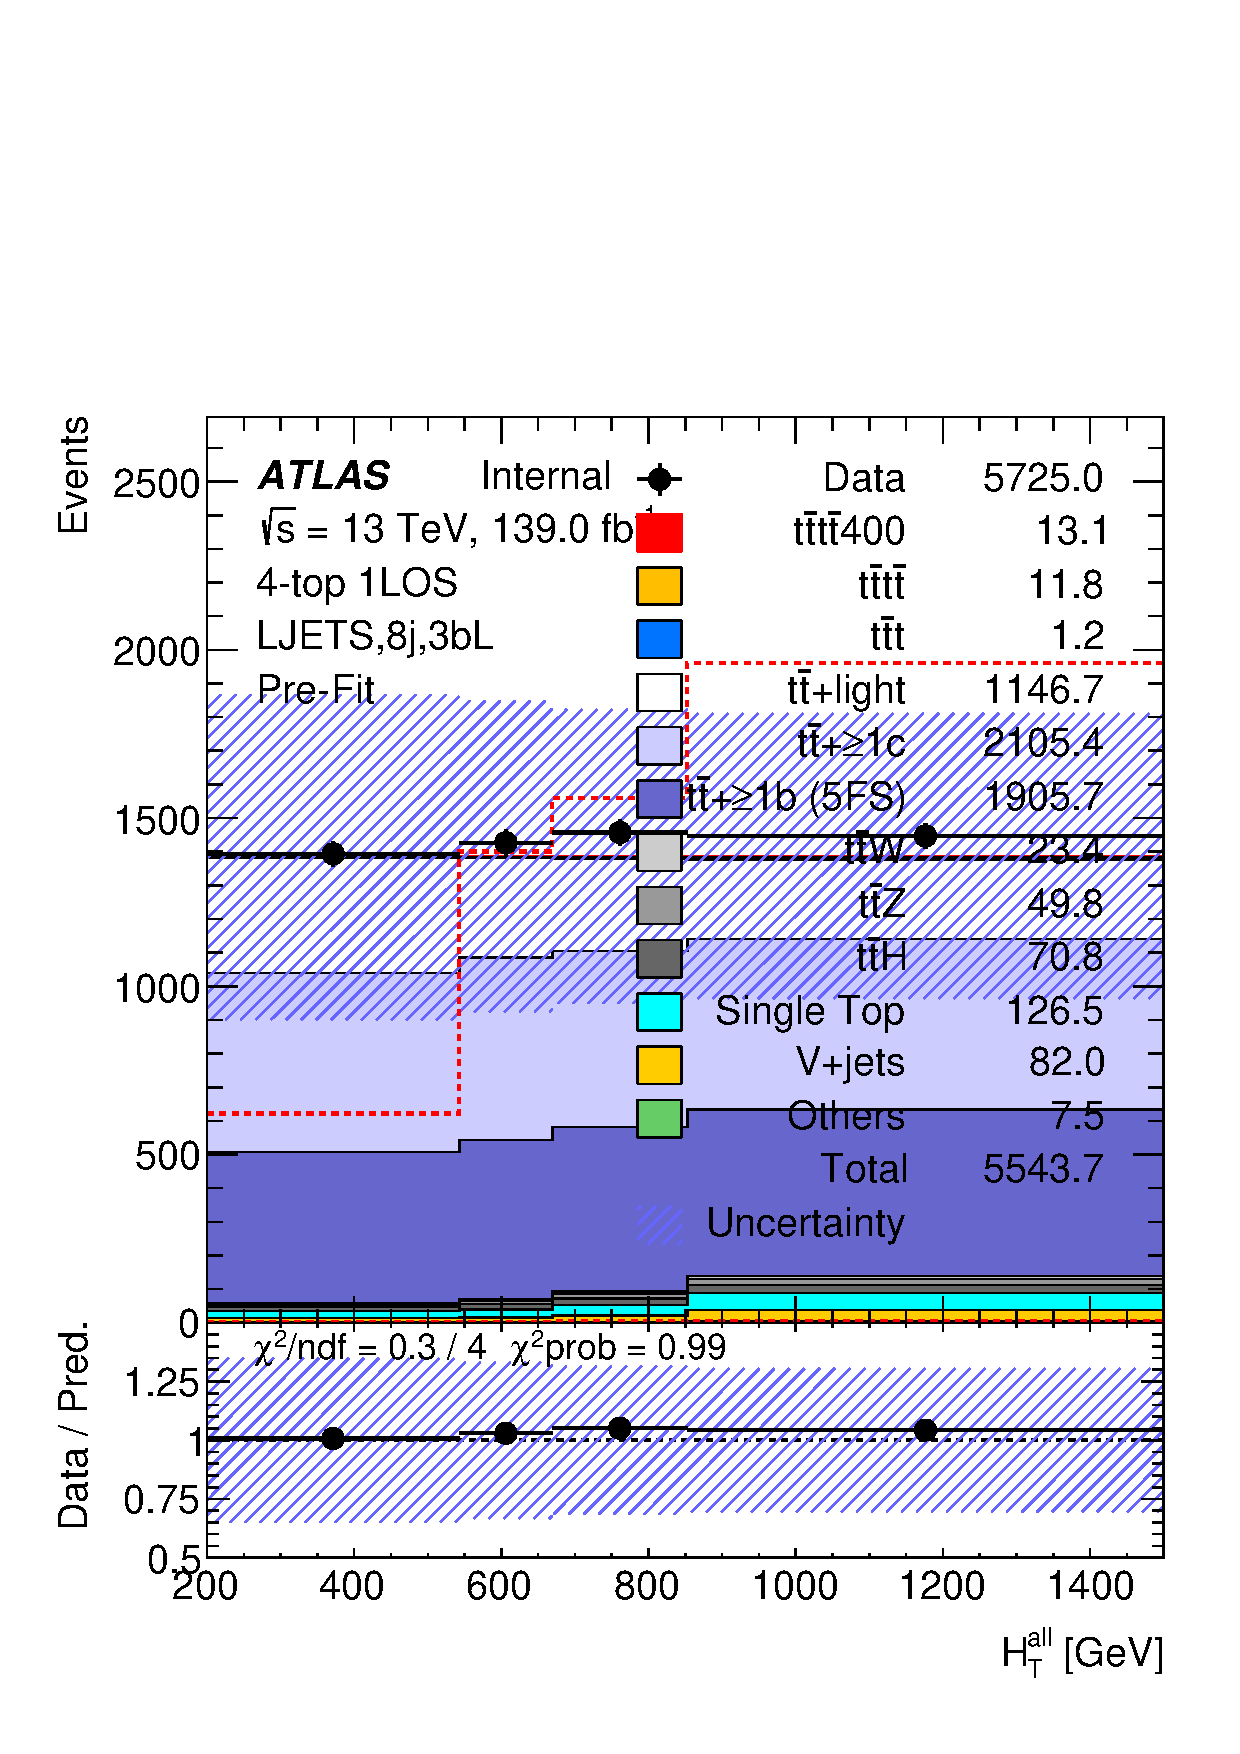
\includegraphics[width=0.23 \textwidth]{figures/fits/GNN/400/1L/data_unblindedSplusB/Plots/ljets_8j3bL.pdf} &
        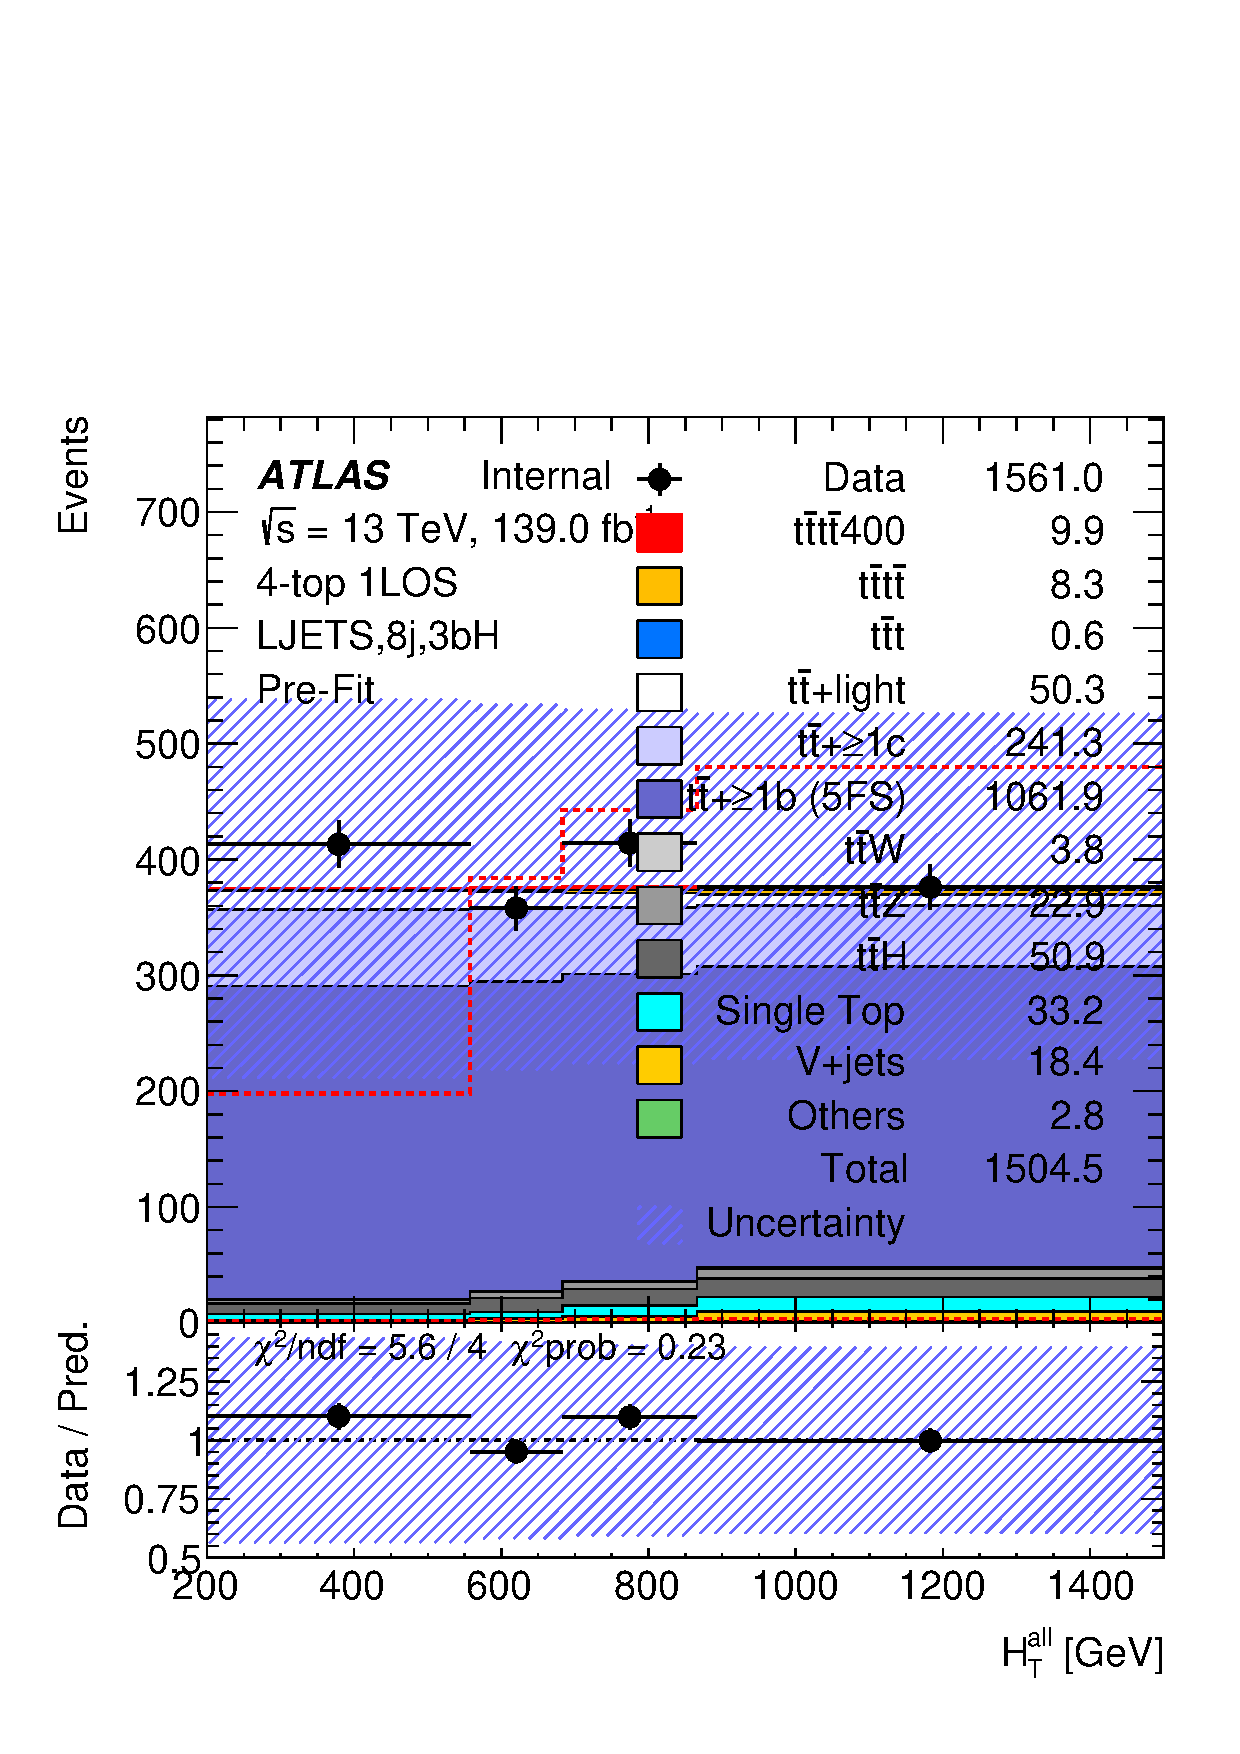
\includegraphics[width=0.23 \textwidth]{figures/fits/GNN/400/1L/data_unblindedSplusB/Plots/ljets_8j3bH.pdf} &
        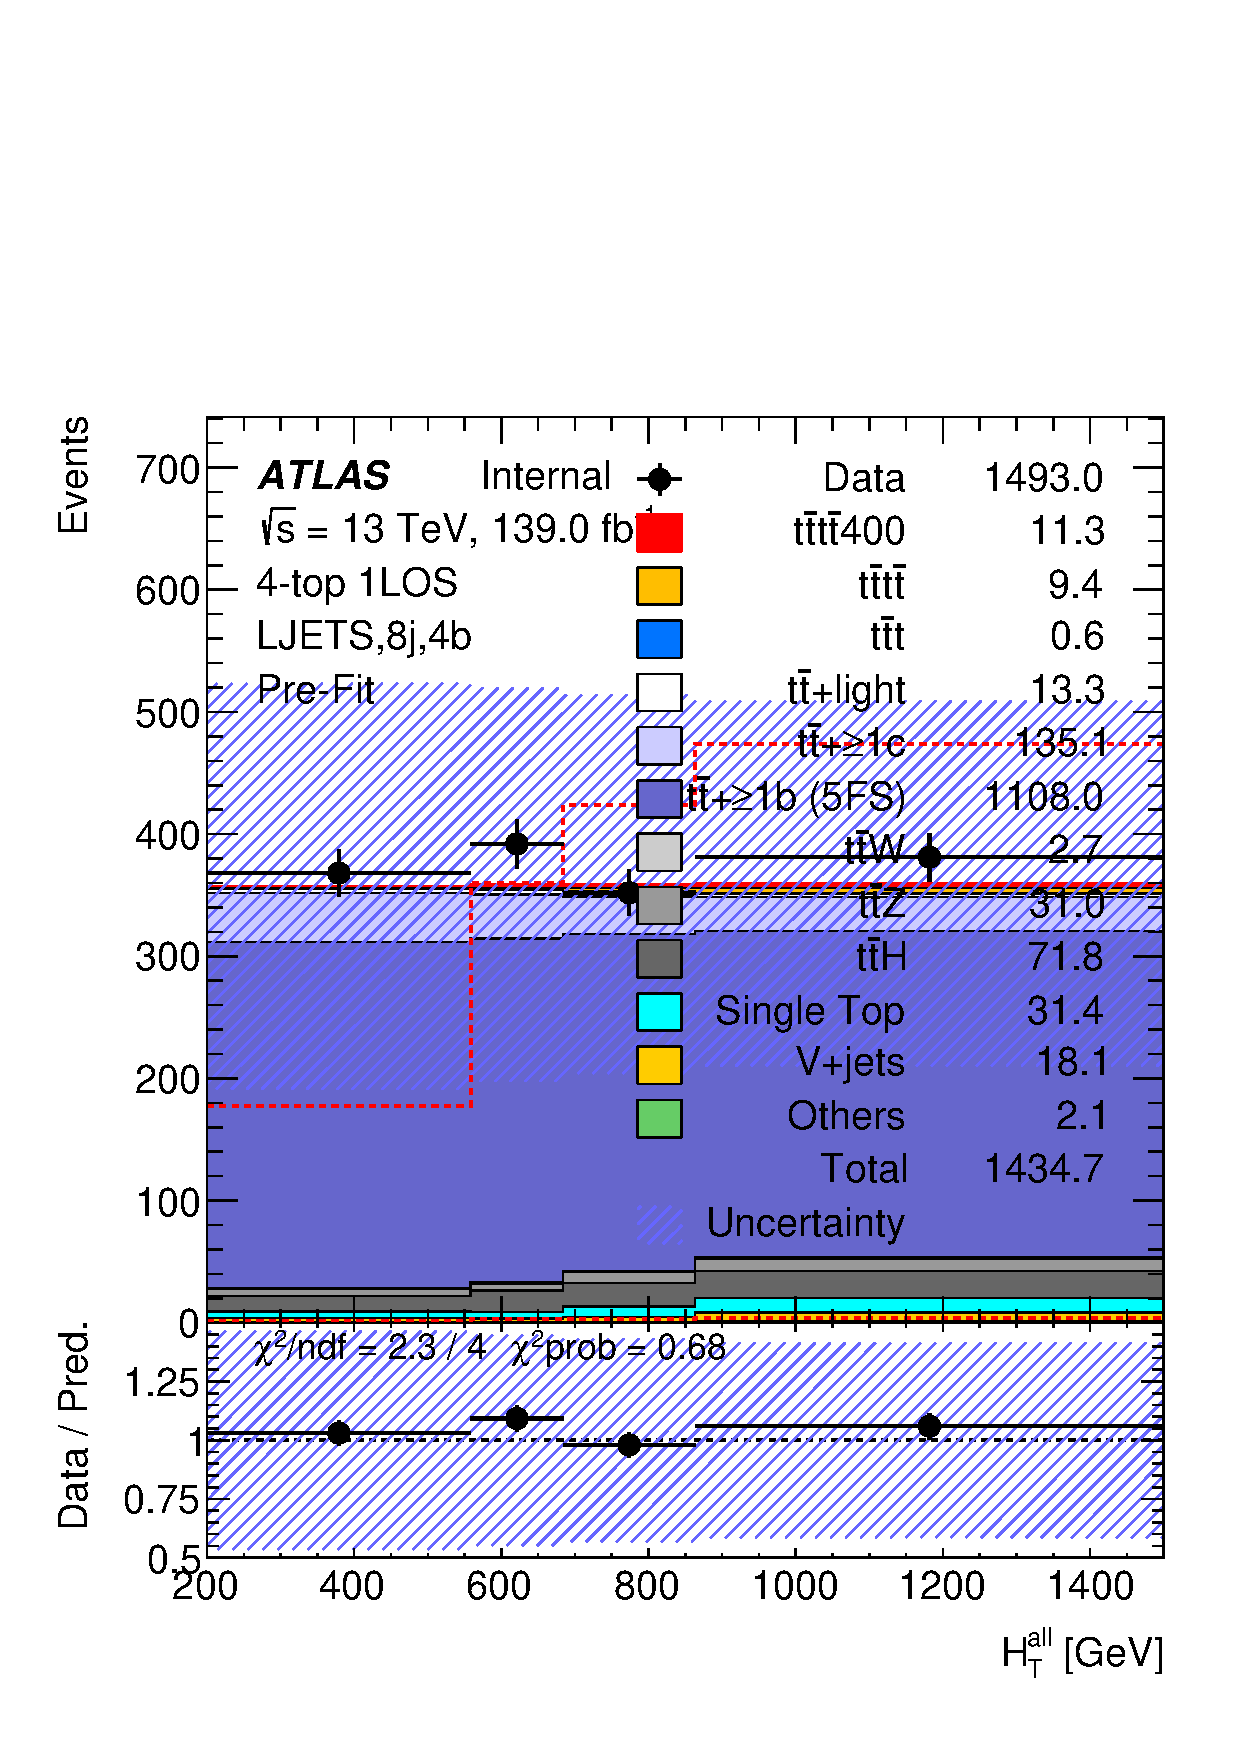
\includegraphics[width=0.23 \textwidth]{figures/fits/GNN/400/1L/data_unblindedSplusB/Plots/ljets_8j4b.pdf} &
        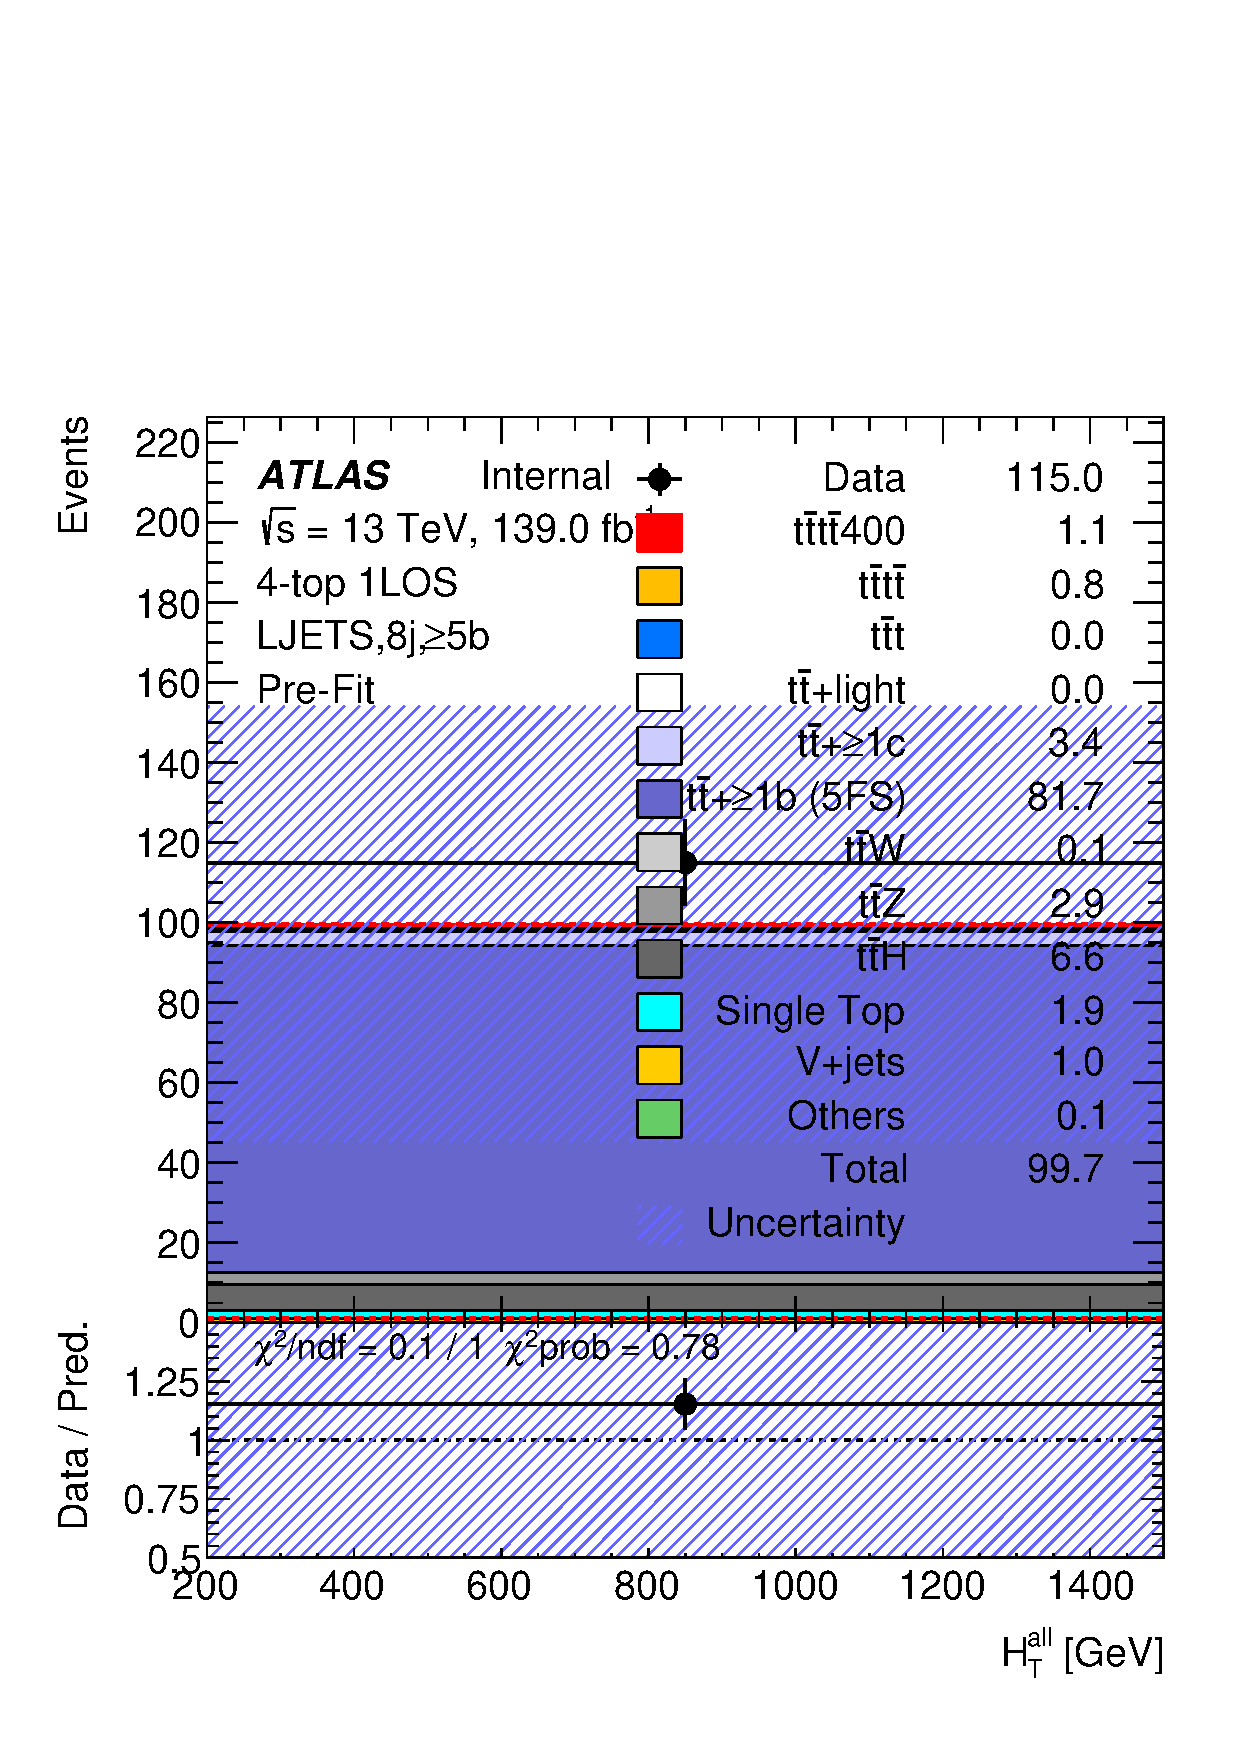
\includegraphics[width=0.23 \textwidth]{figures/fits/GNN/400/1L/data_unblindedSplusB/Plots/ljets_8jge5b.pdf}\\

        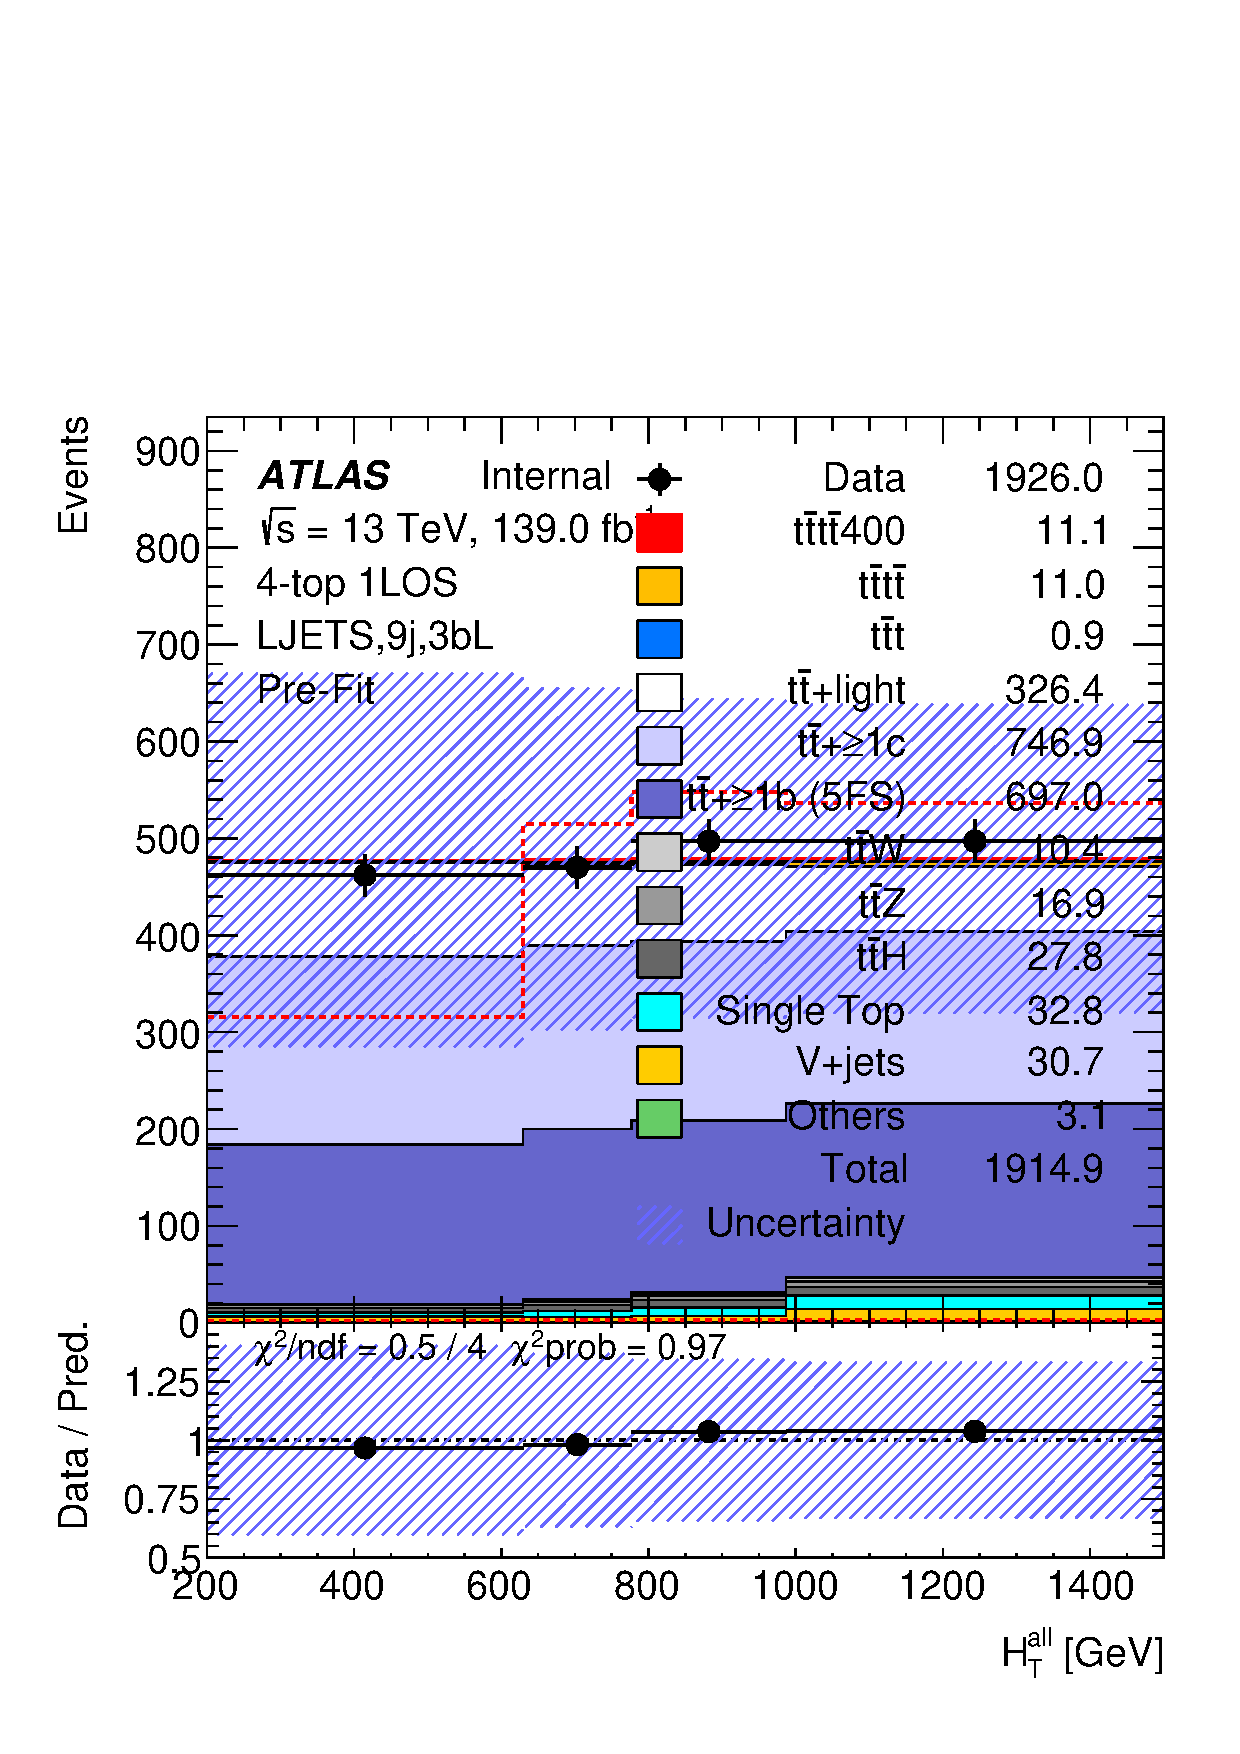
\includegraphics[width=0.23 \textwidth]{figures/fits/GNN/400/1L/data_unblindedSplusB/Plots/ljets_9j3bL.pdf} &
        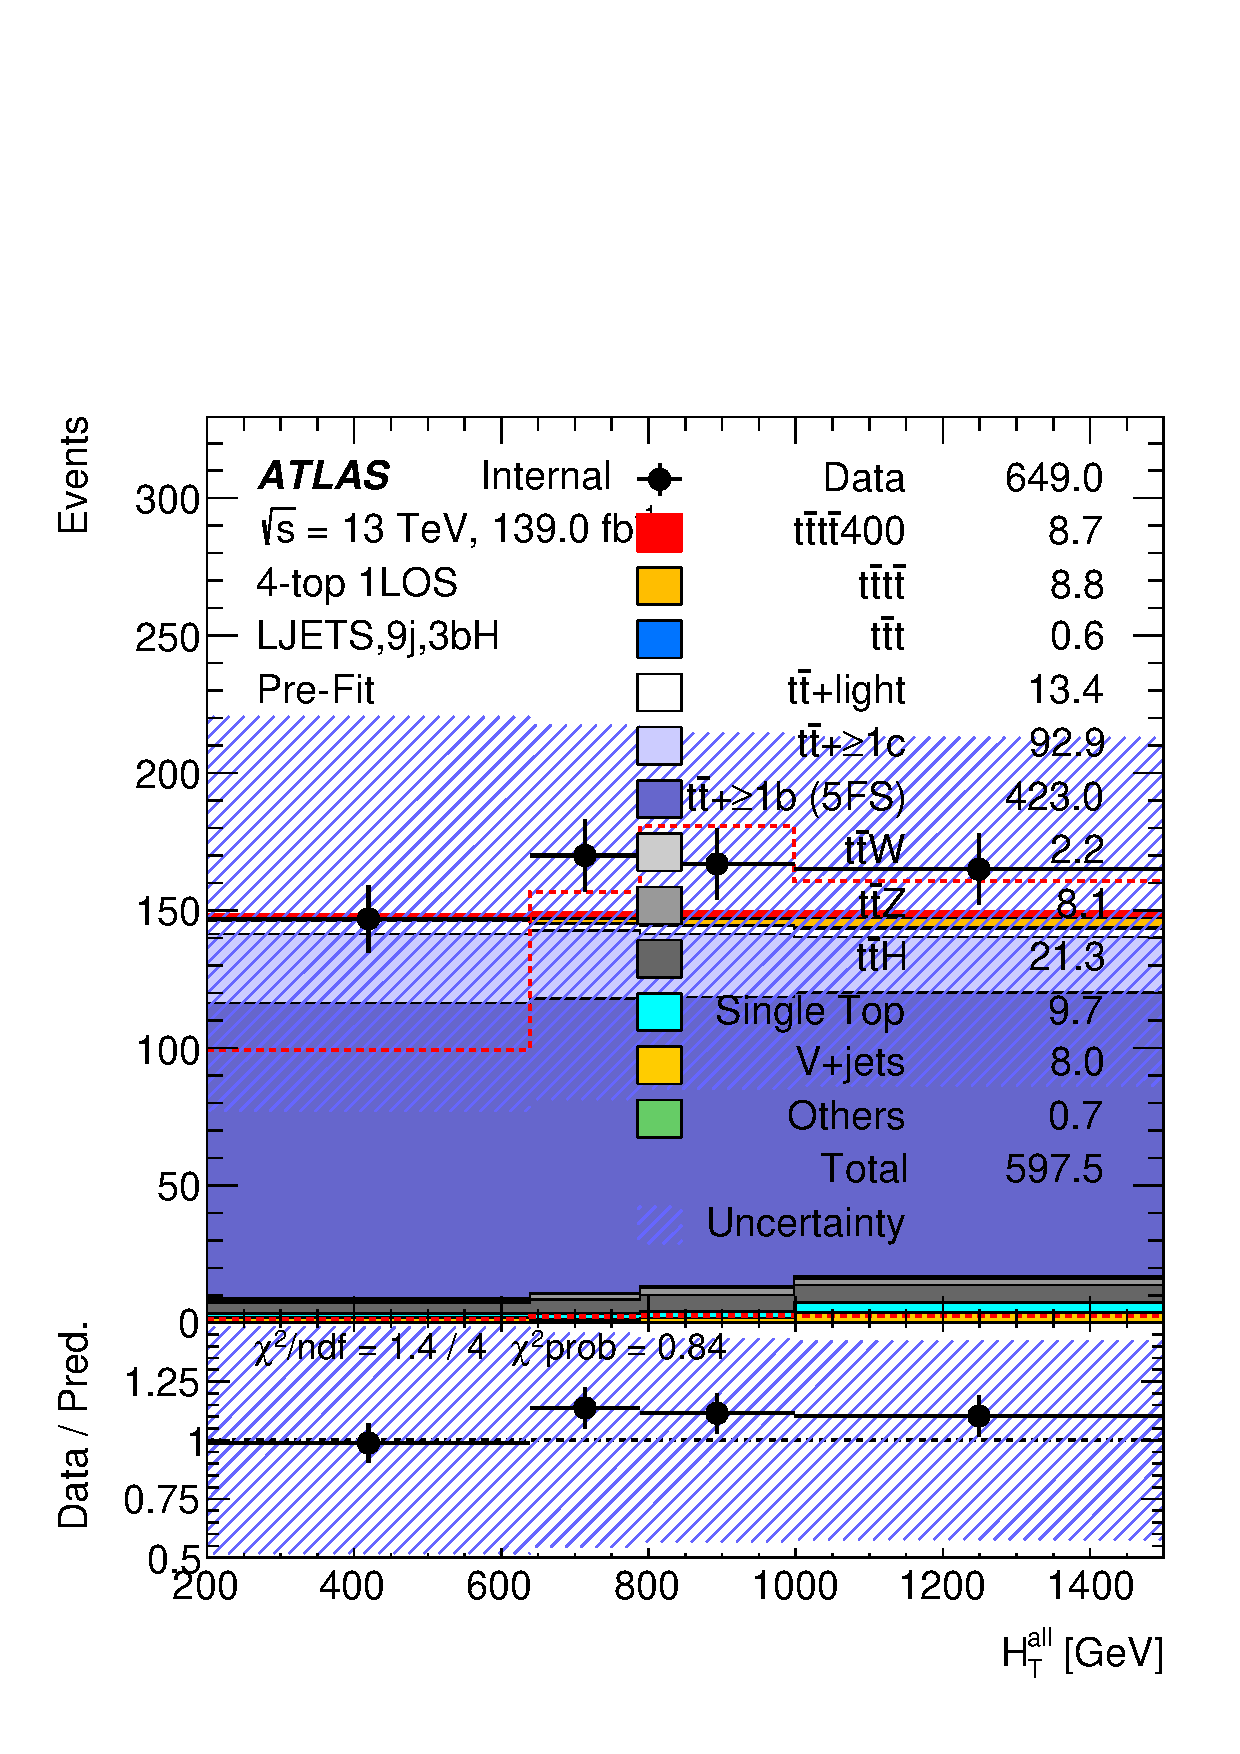
\includegraphics[width=0.23 \textwidth]{figures/fits/GNN/400/1L/data_unblindedSplusB/Plots/ljets_9j3bH.pdf} &
        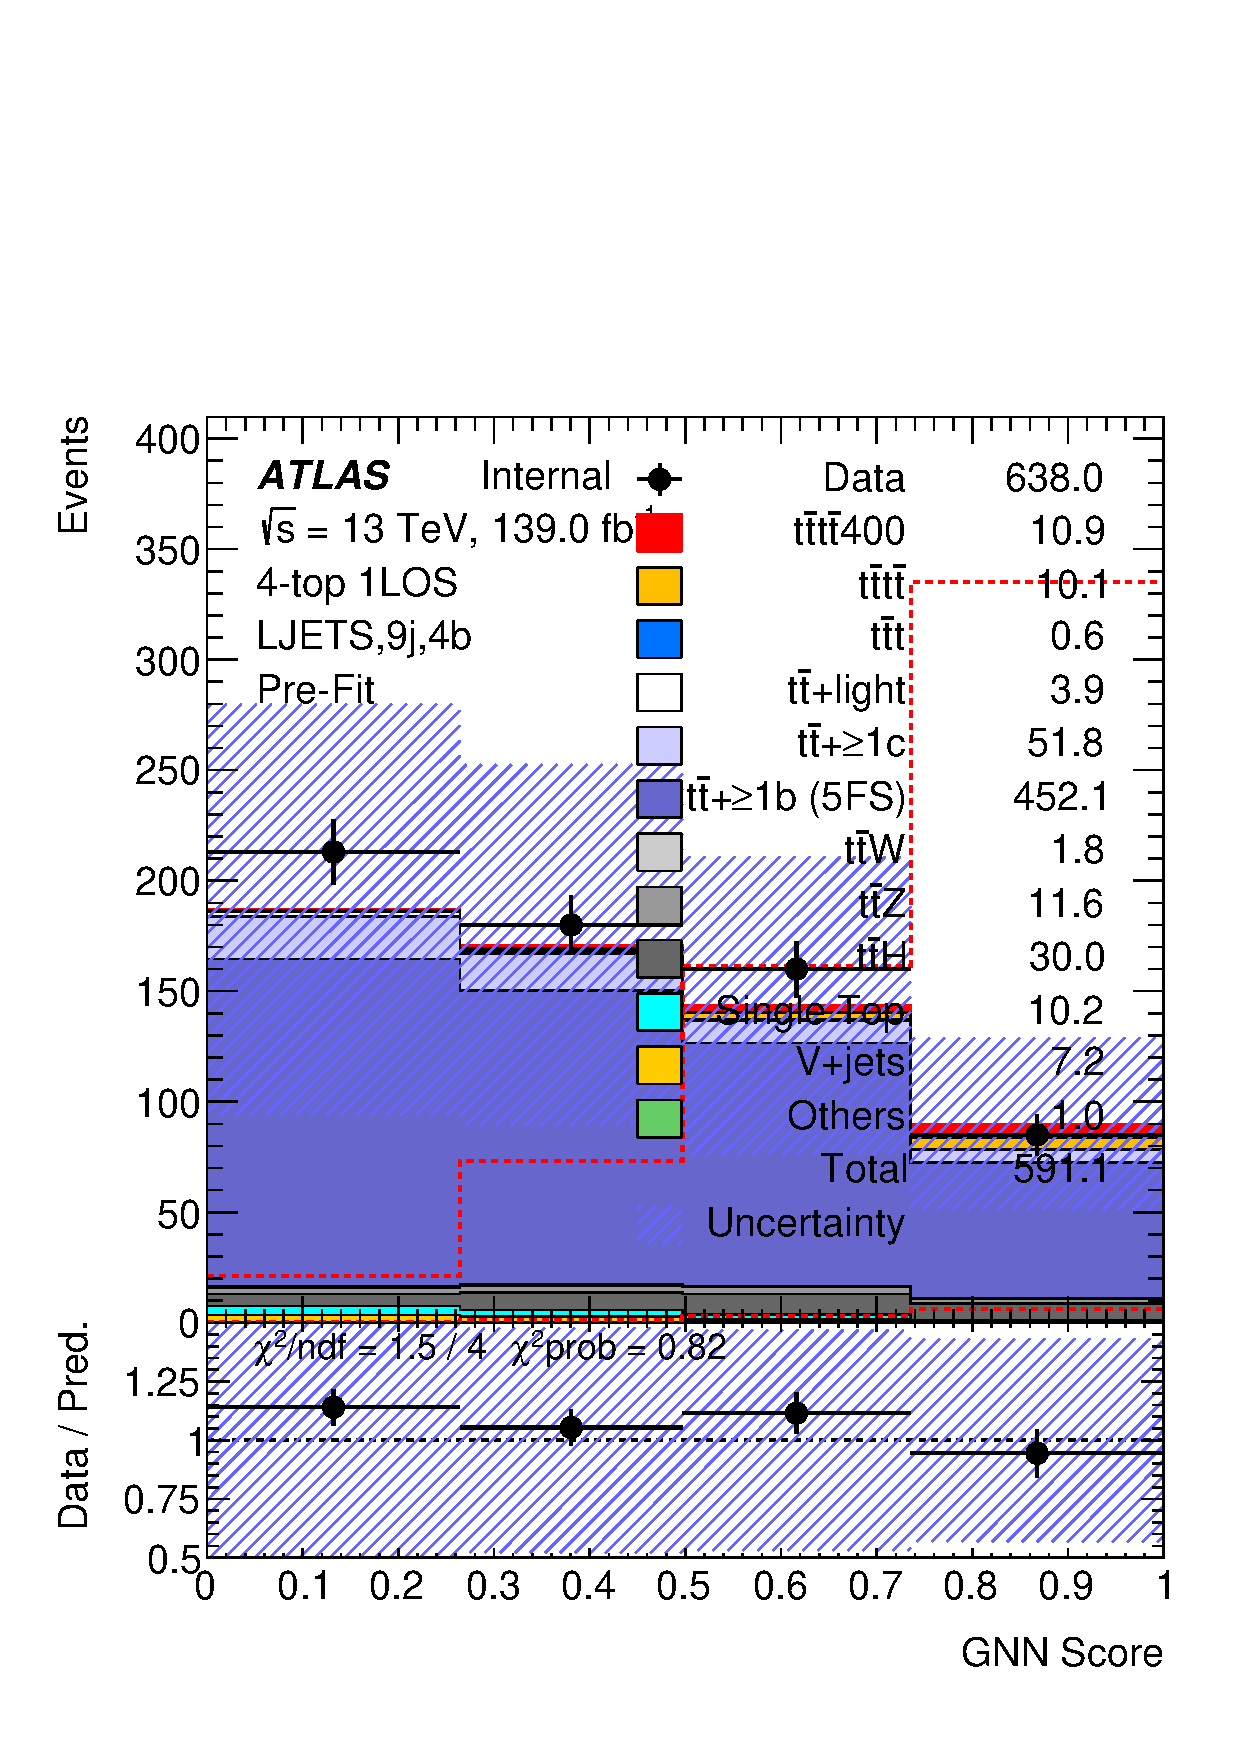
\includegraphics[width=0.23 \textwidth]{figures/fits/GNN/400/1L/data_unblindedSplusB/Plots/ljets_9j4b.pdf} &
        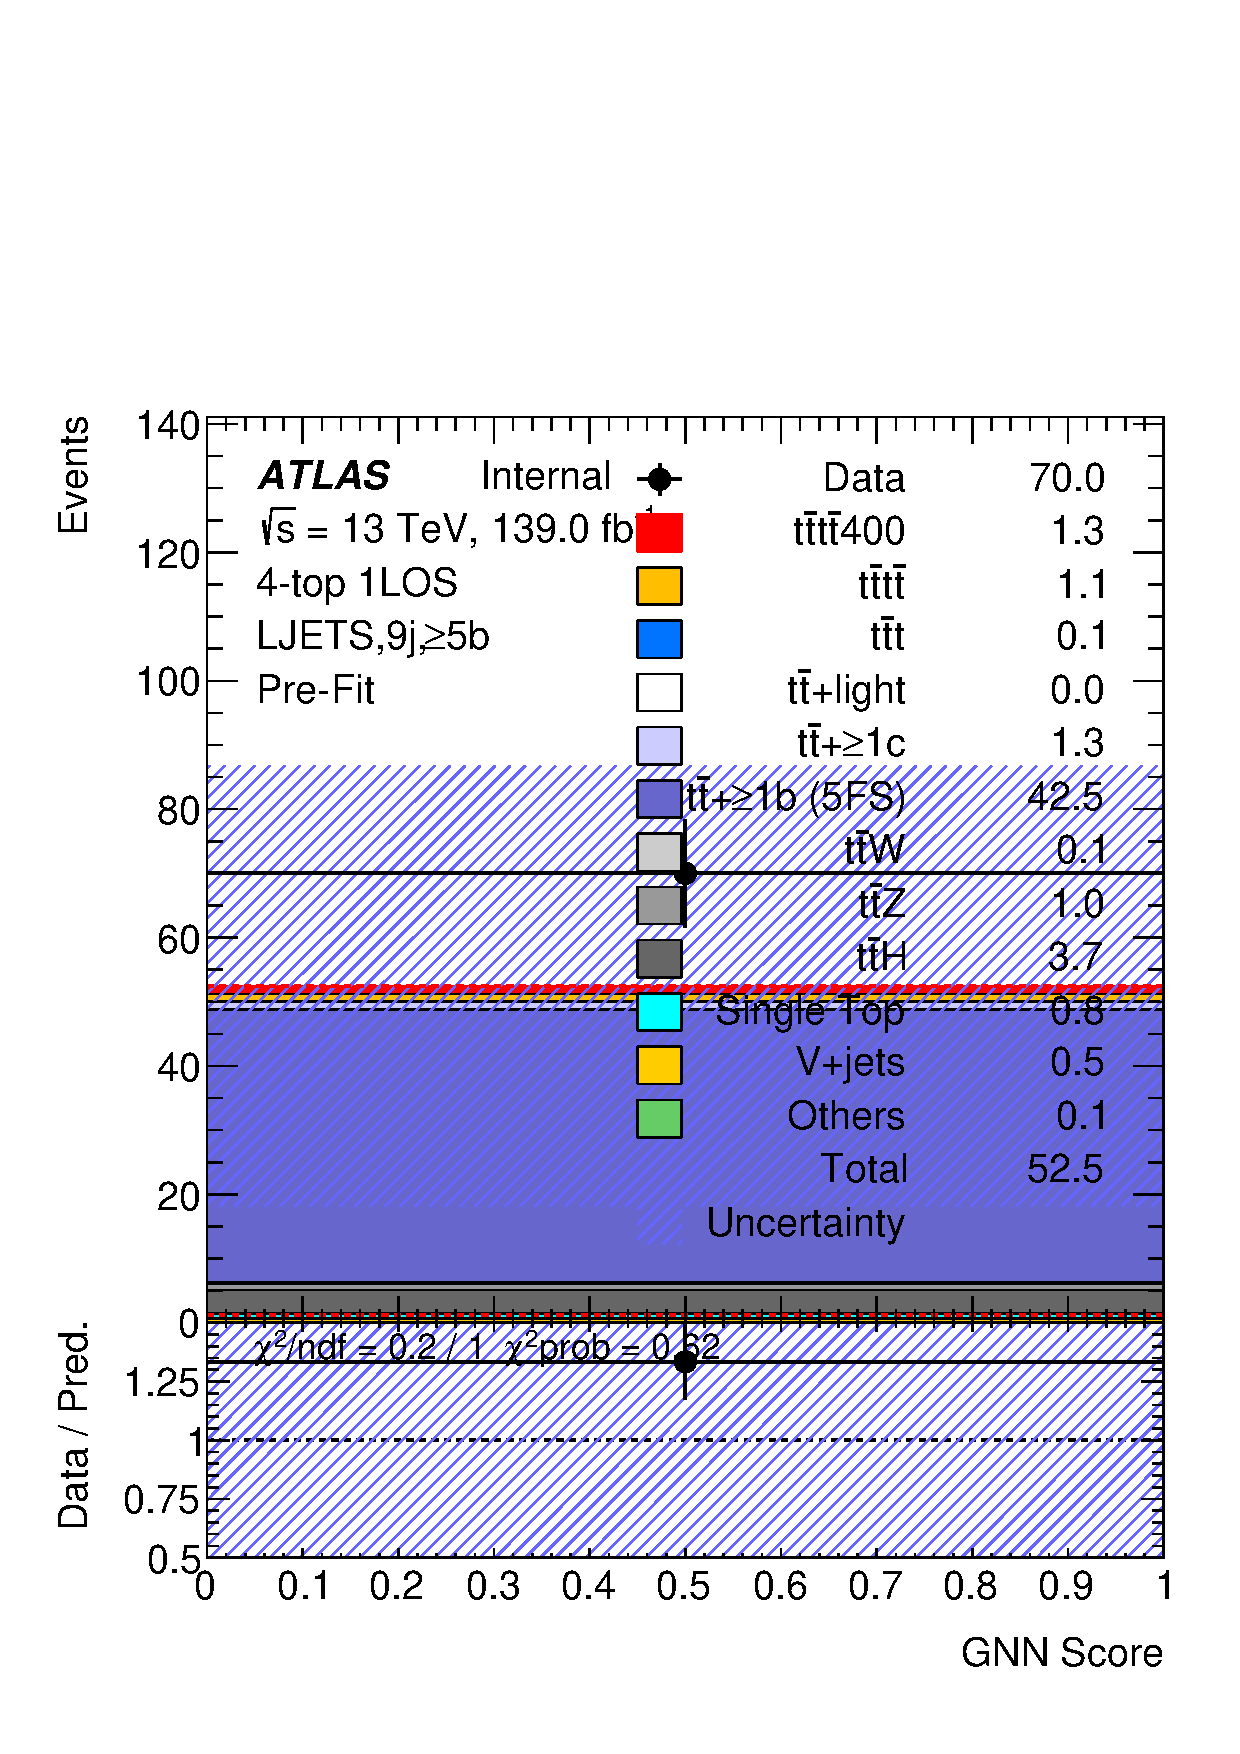
\includegraphics[width=0.23 \textwidth]{figures/fits/GNN/400/1L/data_unblindedSplusB/Plots/ljets_9jge5b.pdf} \\

        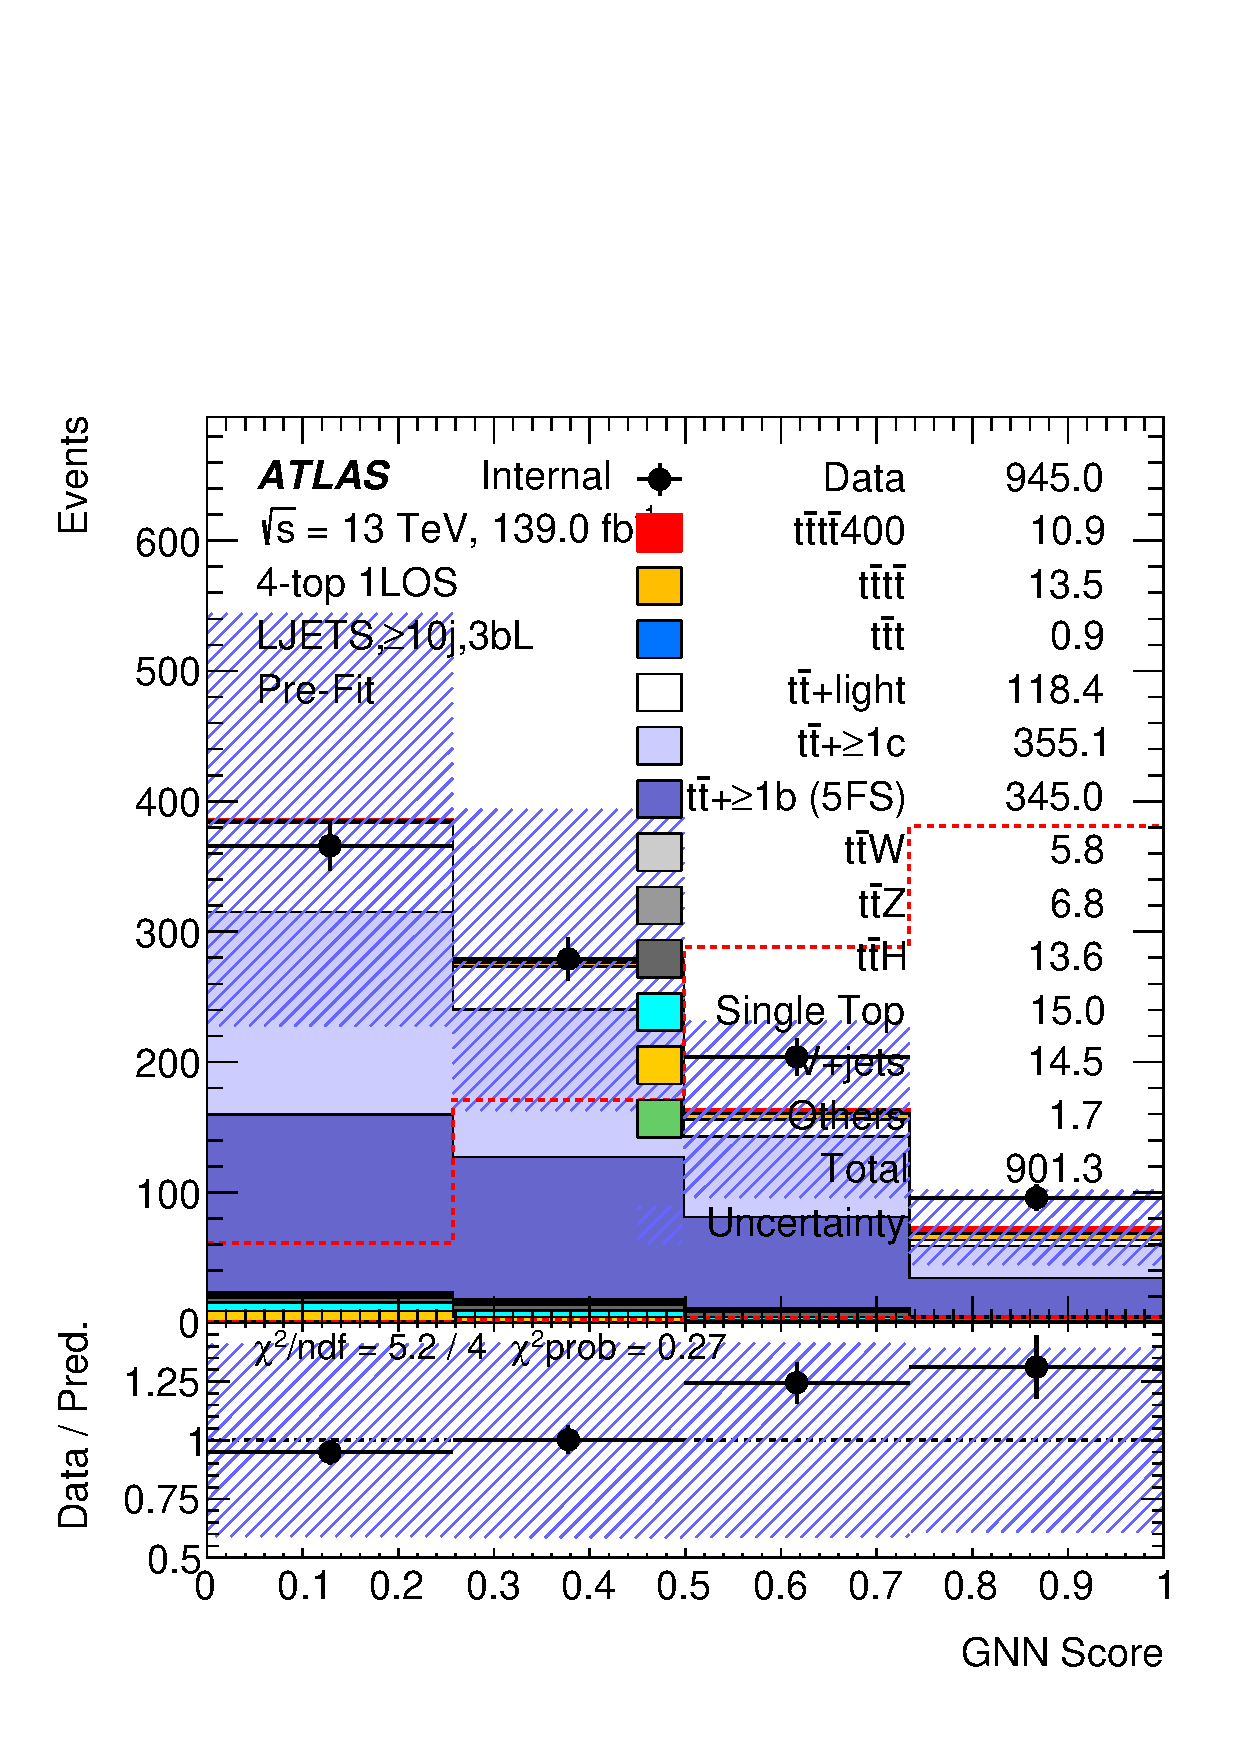
\includegraphics[width=0.23 \textwidth]{figures/fits/GNN/400/1L/data_unblindedSplusB/Plots/ljets_ge10j3bL.pdf} &
        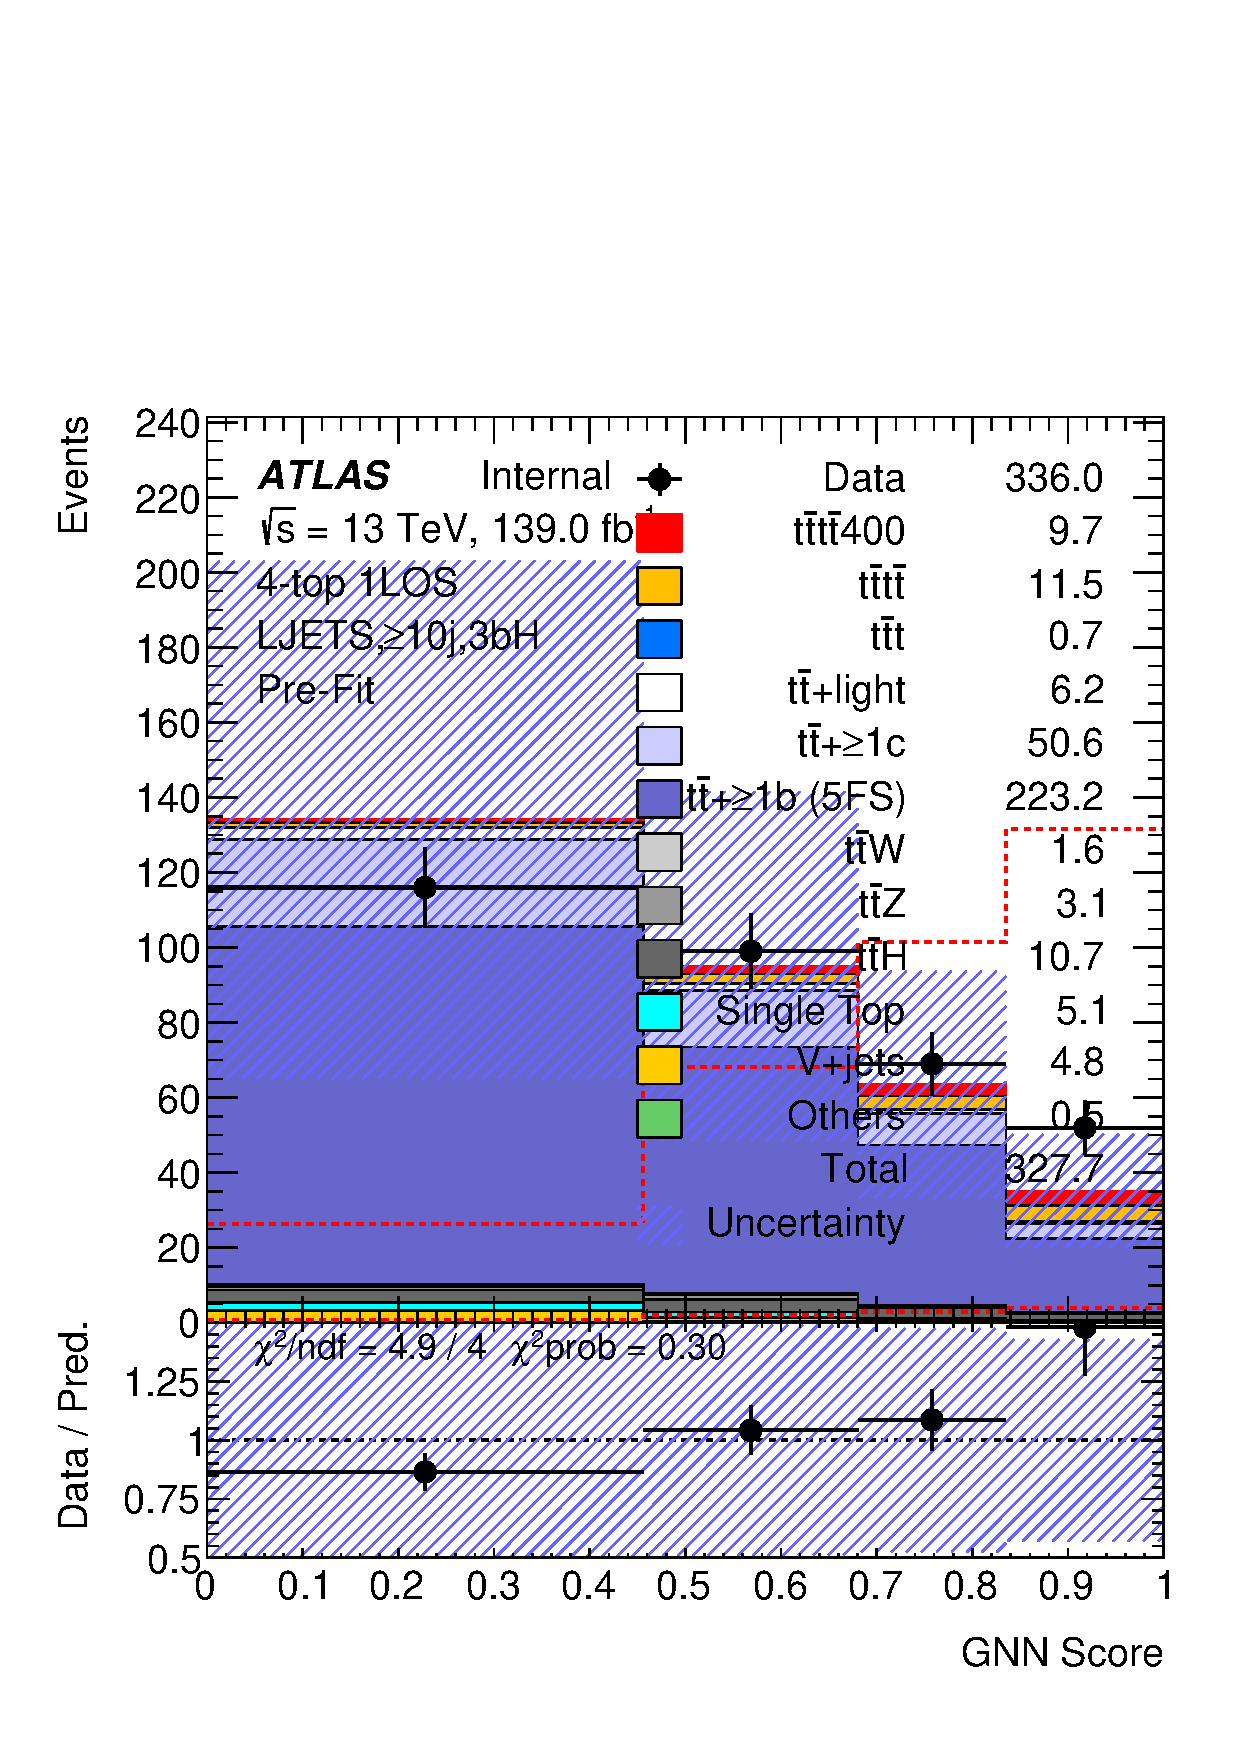
\includegraphics[width=0.23 \textwidth]{figures/fits/GNN/400/1L/data_unblindedSplusB/Plots/ljets_ge10j3bH.pdf} &
        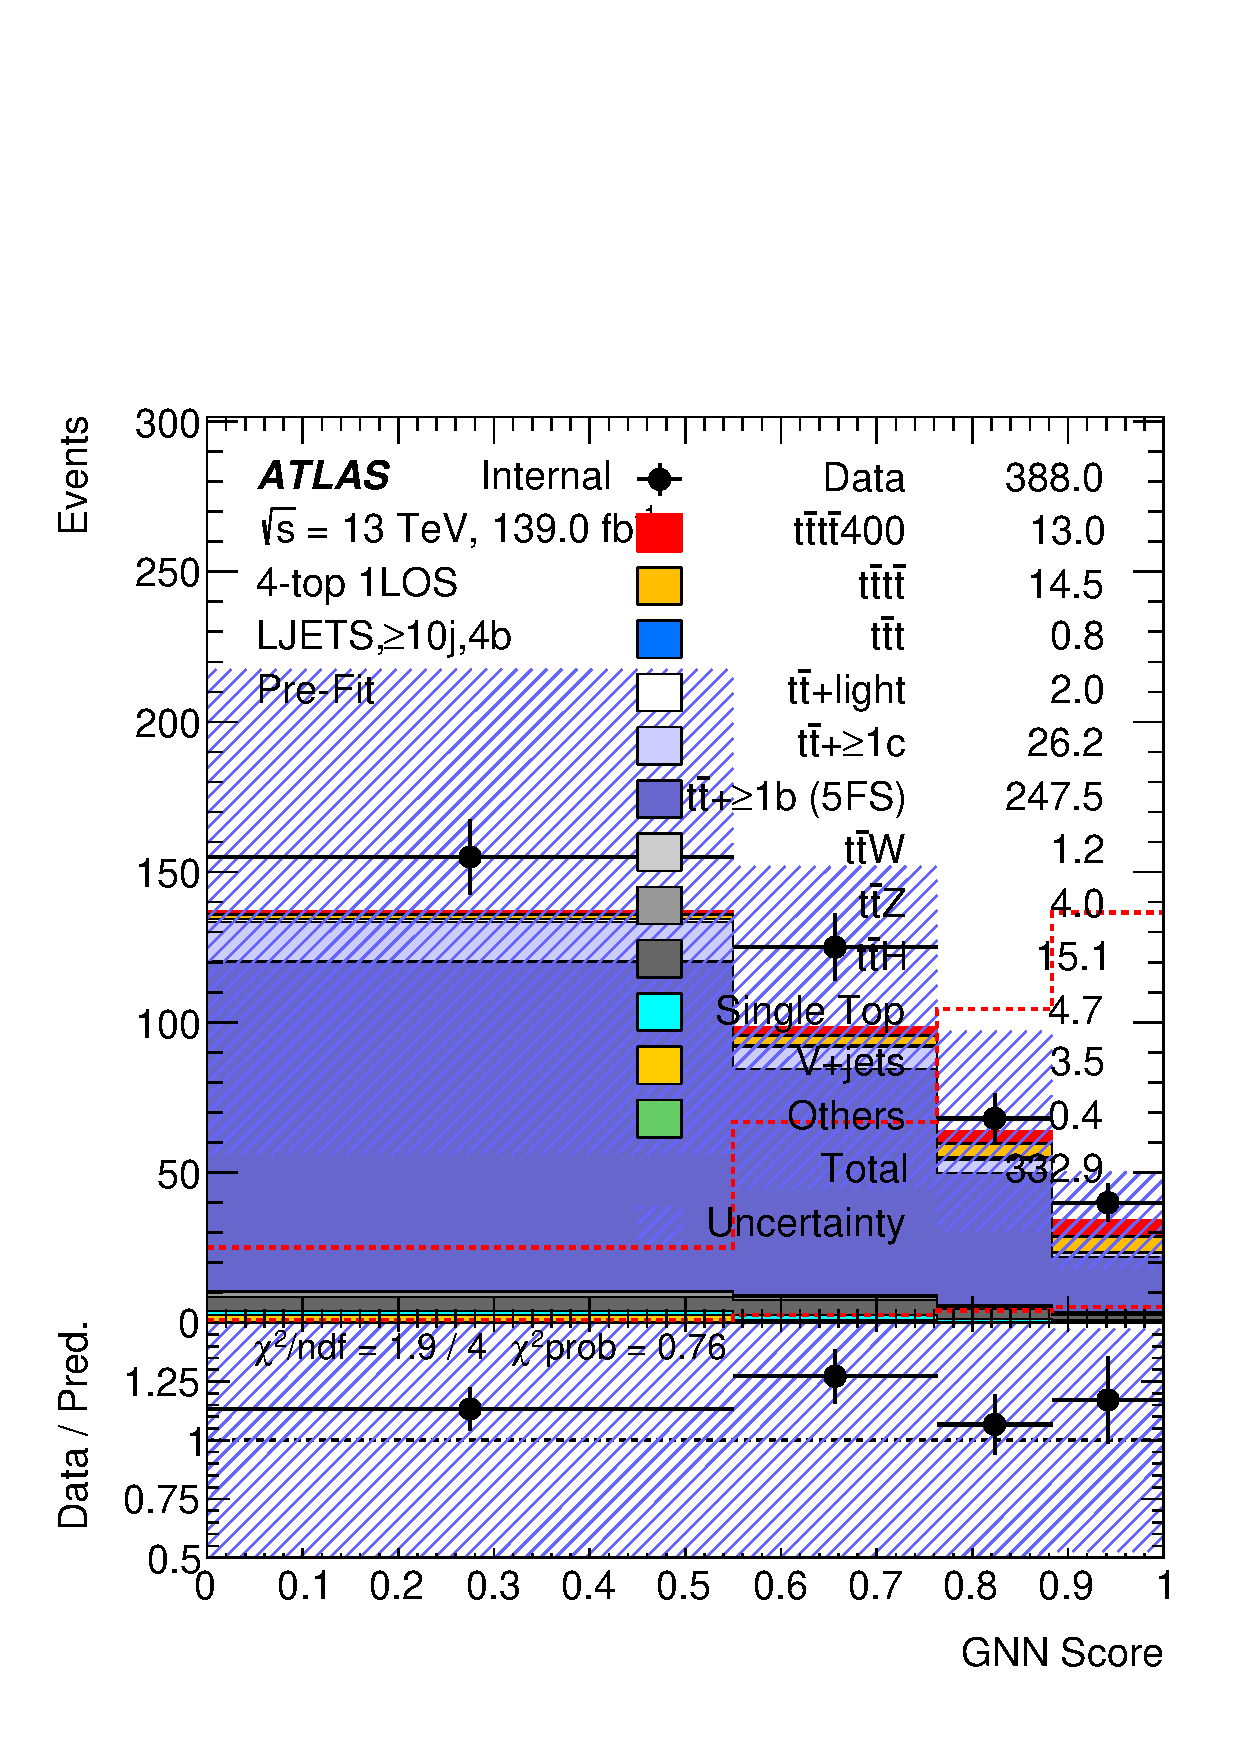
\includegraphics[width=0.23 \textwidth]{figures/fits/GNN/400/1L/data_unblindedSplusB/Plots/ljets_ge10j4b.pdf} &
        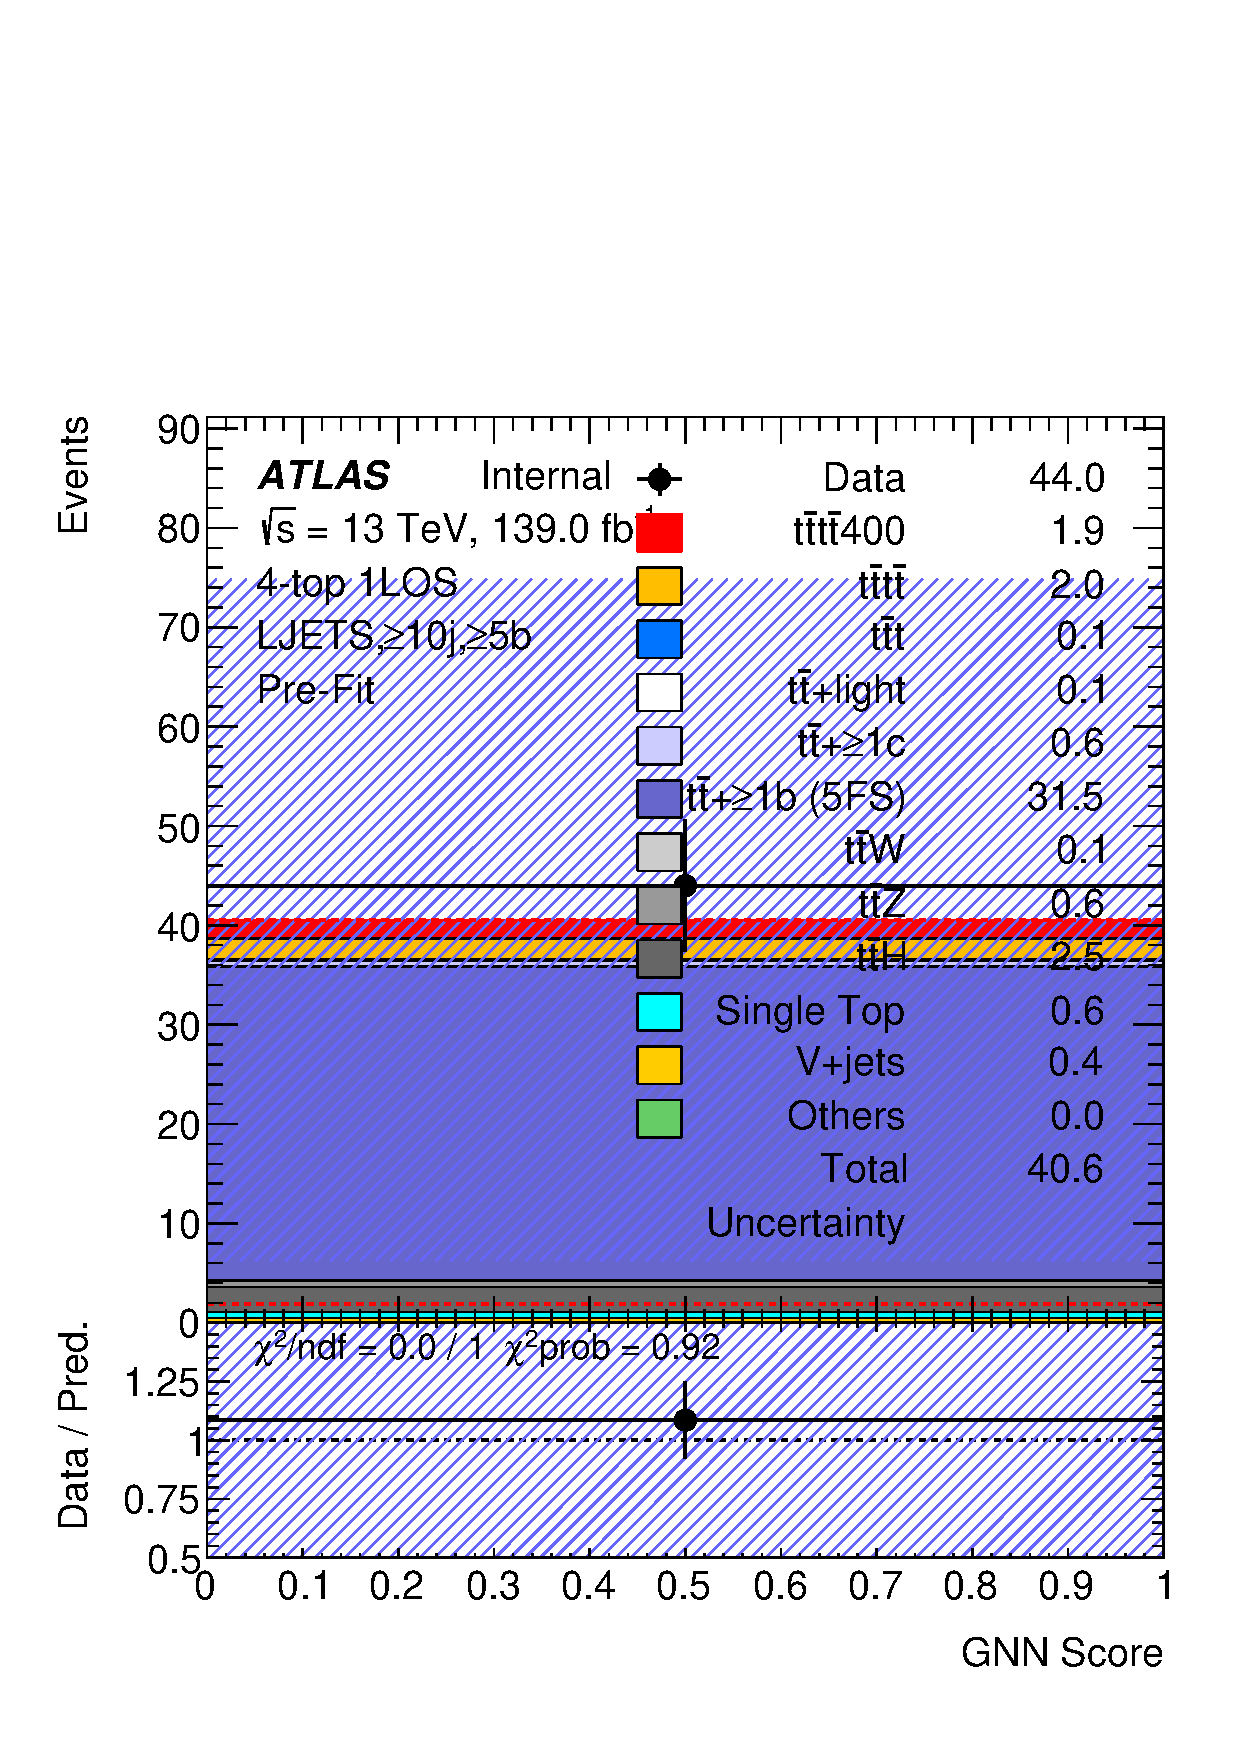
\includegraphics[width=0.23 \textwidth]{figures/fits/GNN/400/1L/data_unblindedSplusB/Plots/ljets_ge10jge5b.pdf} \\
        \end{tabular}
        \caption{\label{fig:Prefit_Yields_1L}Pre-fit distributions for 1L channel associated with different signal and background samples, compared with data yields. In general, MC samples and data have good agreement. The signal sample is normalised to a cross-section of 12 fb.}
\end{center}
\end{figure}

\begin{figure}[htbp!]
        \begin{center} \setlength{\tabcolsep}{2.5pt}\footnotesize
        \begin{tabular}{ccc}
        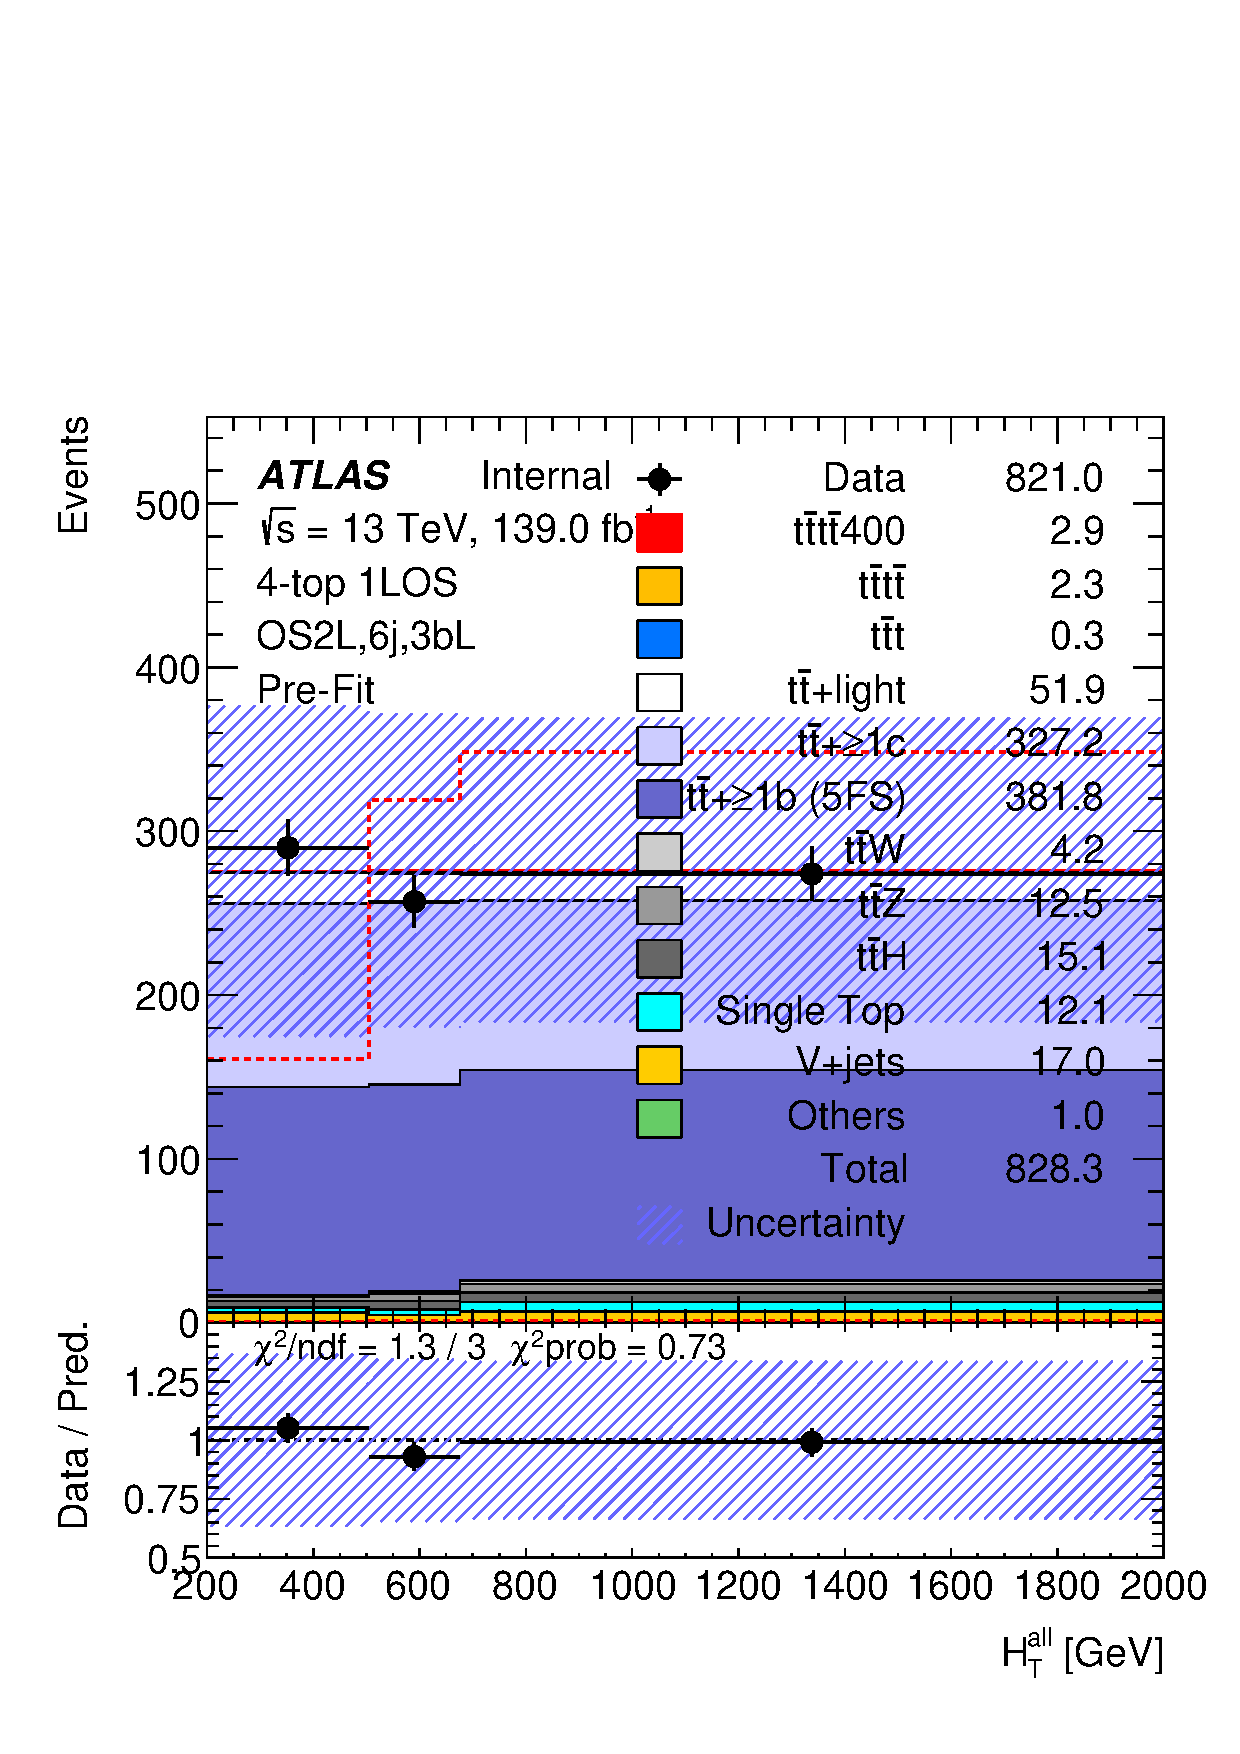
\includegraphics[width=0.31 \textwidth]{figures/fits/GNN/400/2L/data_unblindedSplusB/Plots/os2l_6j3bL.pdf} &
        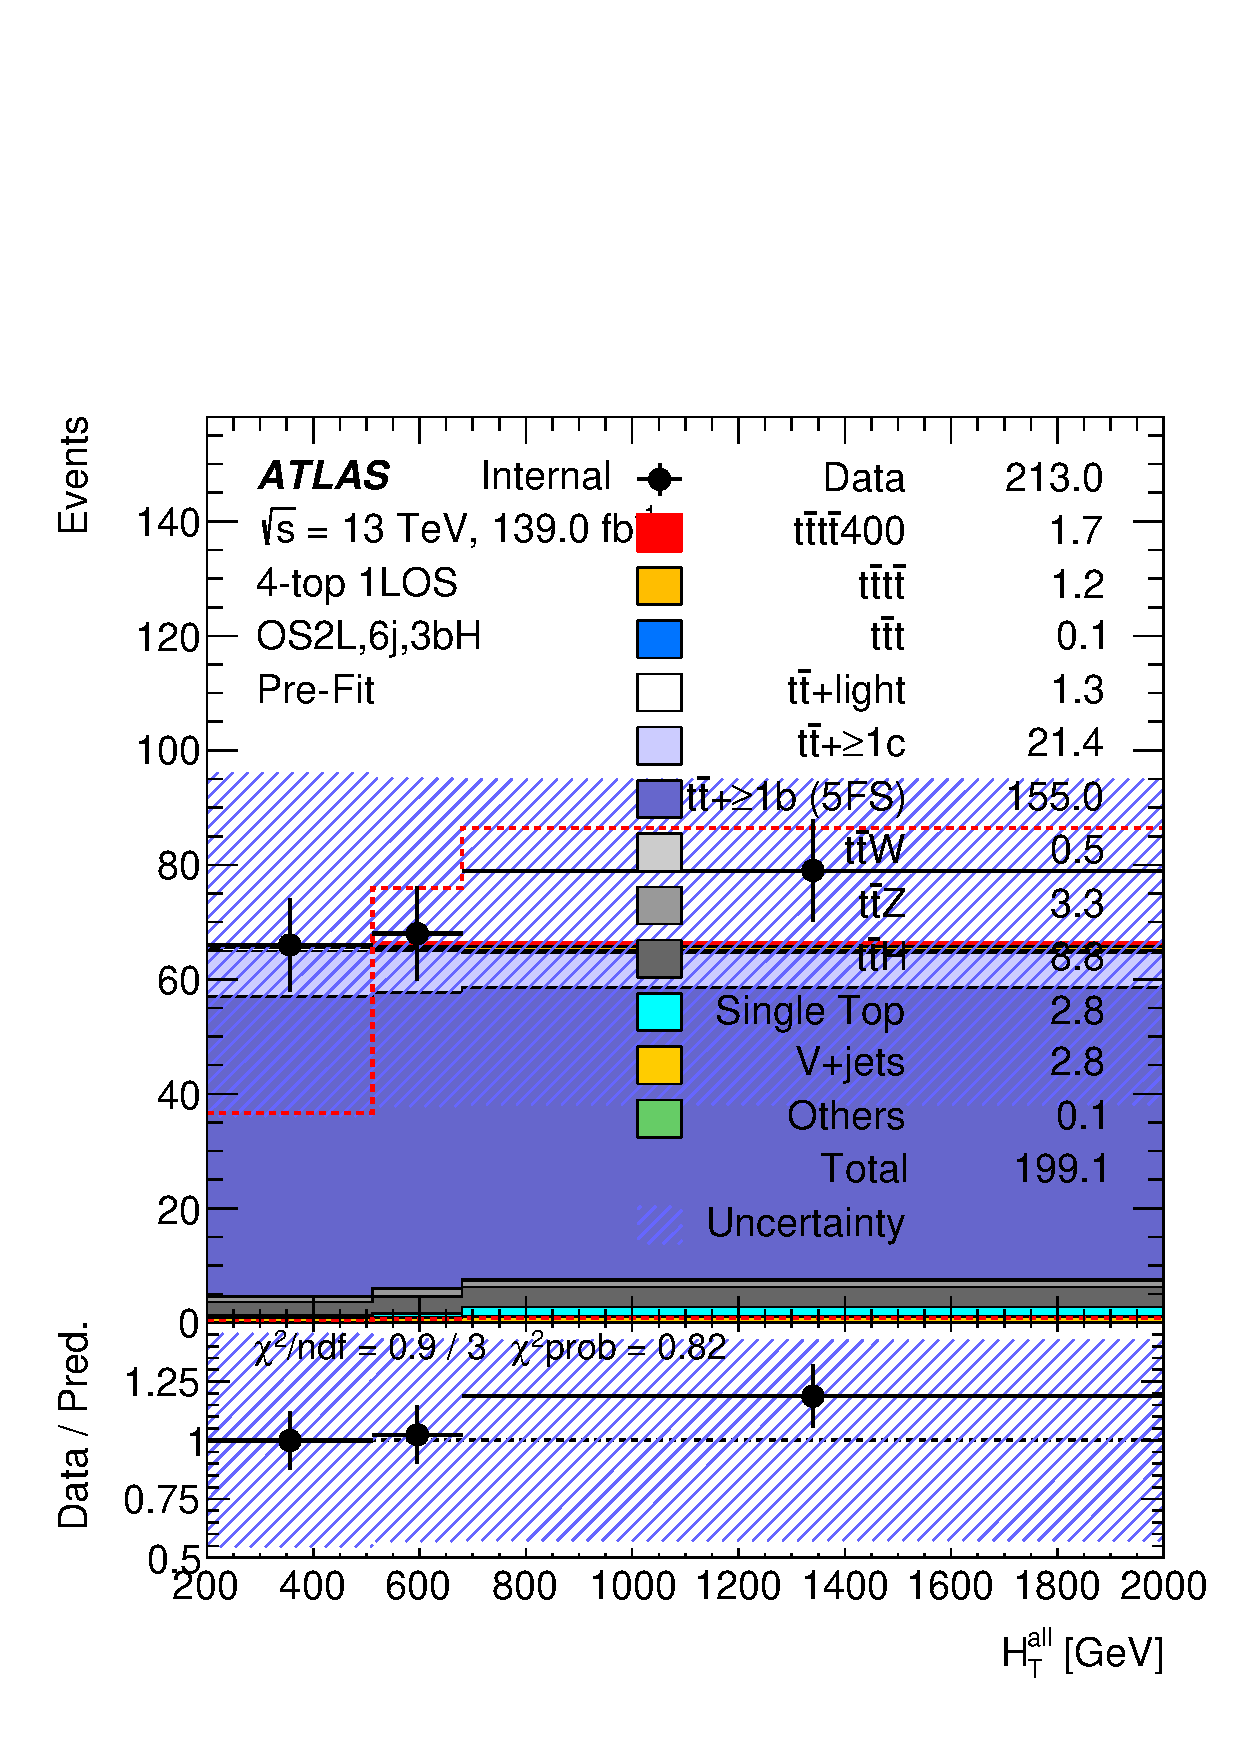
\includegraphics[width=0.31 \textwidth]{figures/fits/GNN/400/2L/data_unblindedSplusB/Plots/os2l_6j3bH.pdf} &
        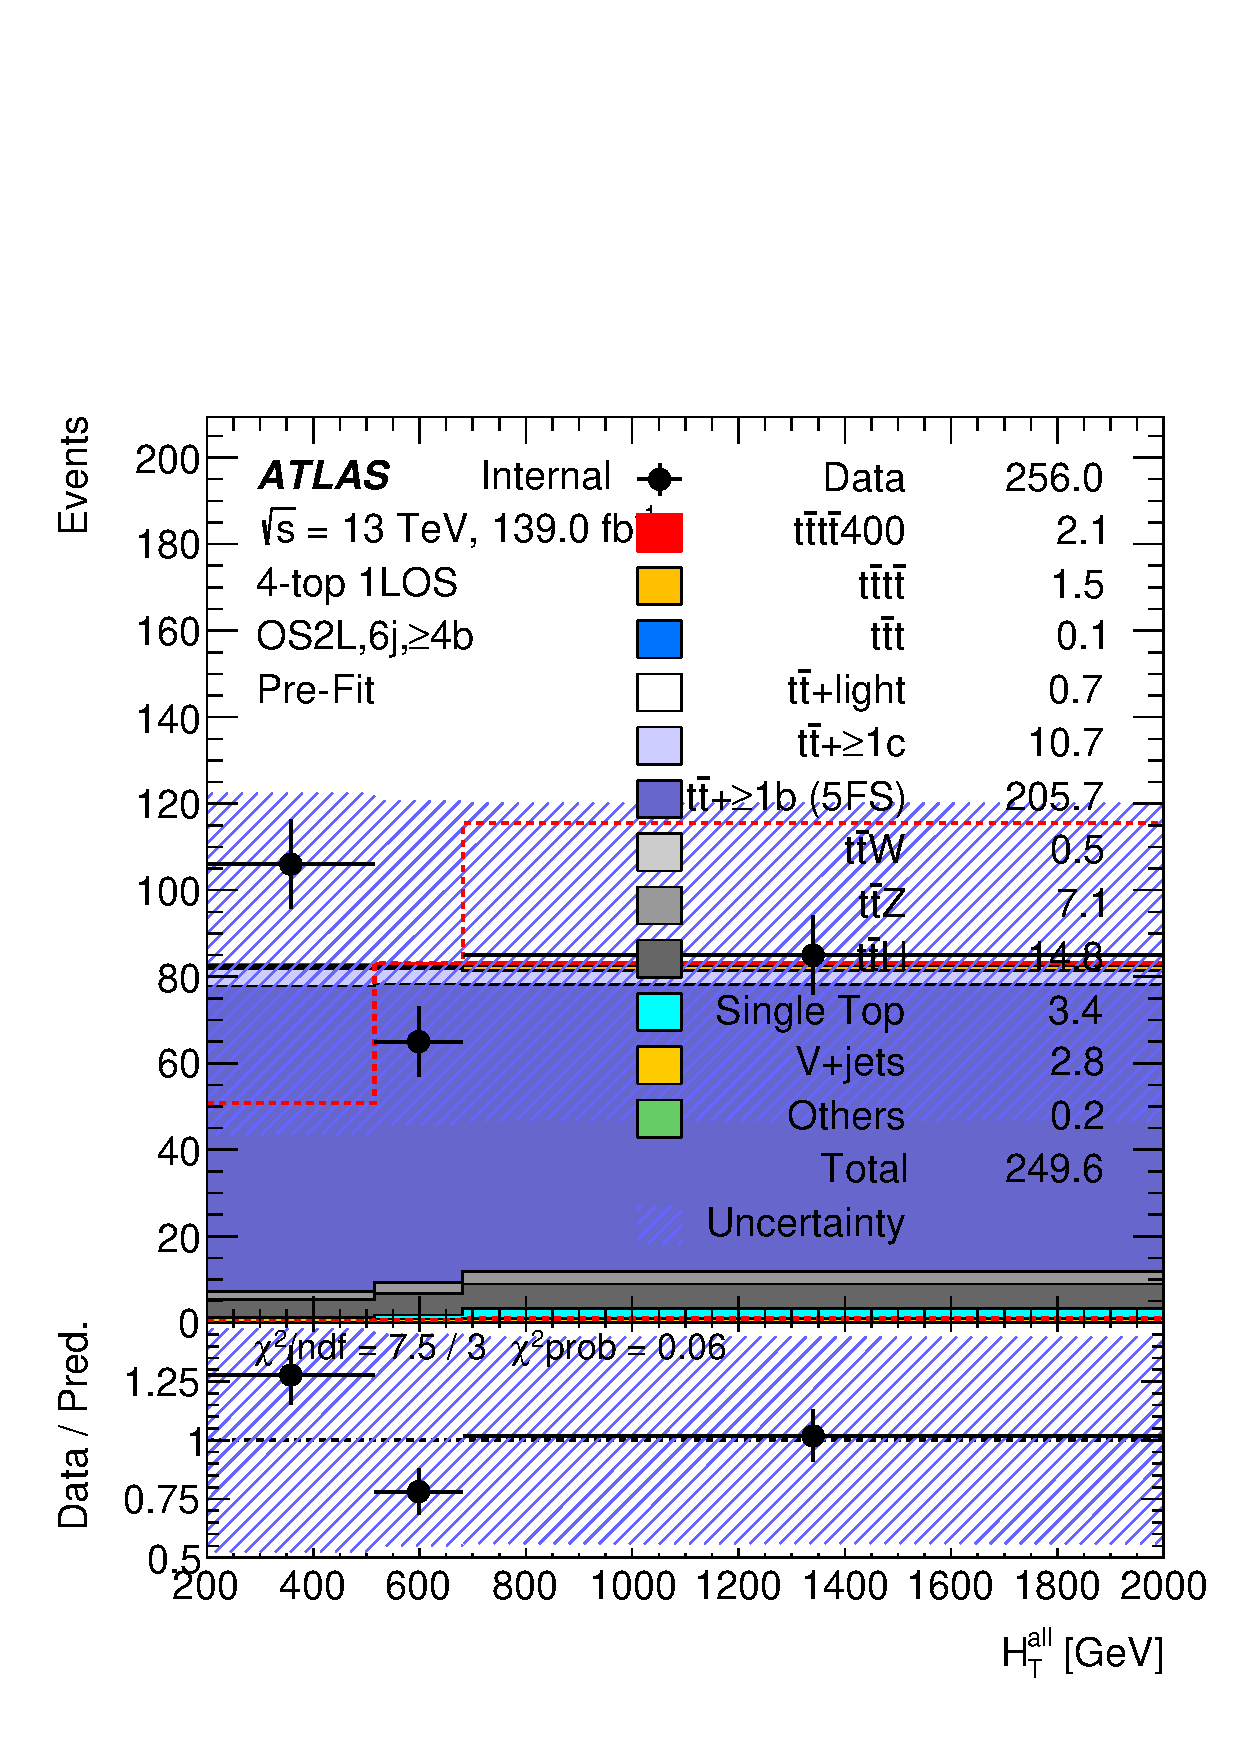
\includegraphics[width=0.31 \textwidth]{figures/fits/GNN/400/2L/data_unblindedSplusB/Plots/os2l_6jge4b.pdf} \\

        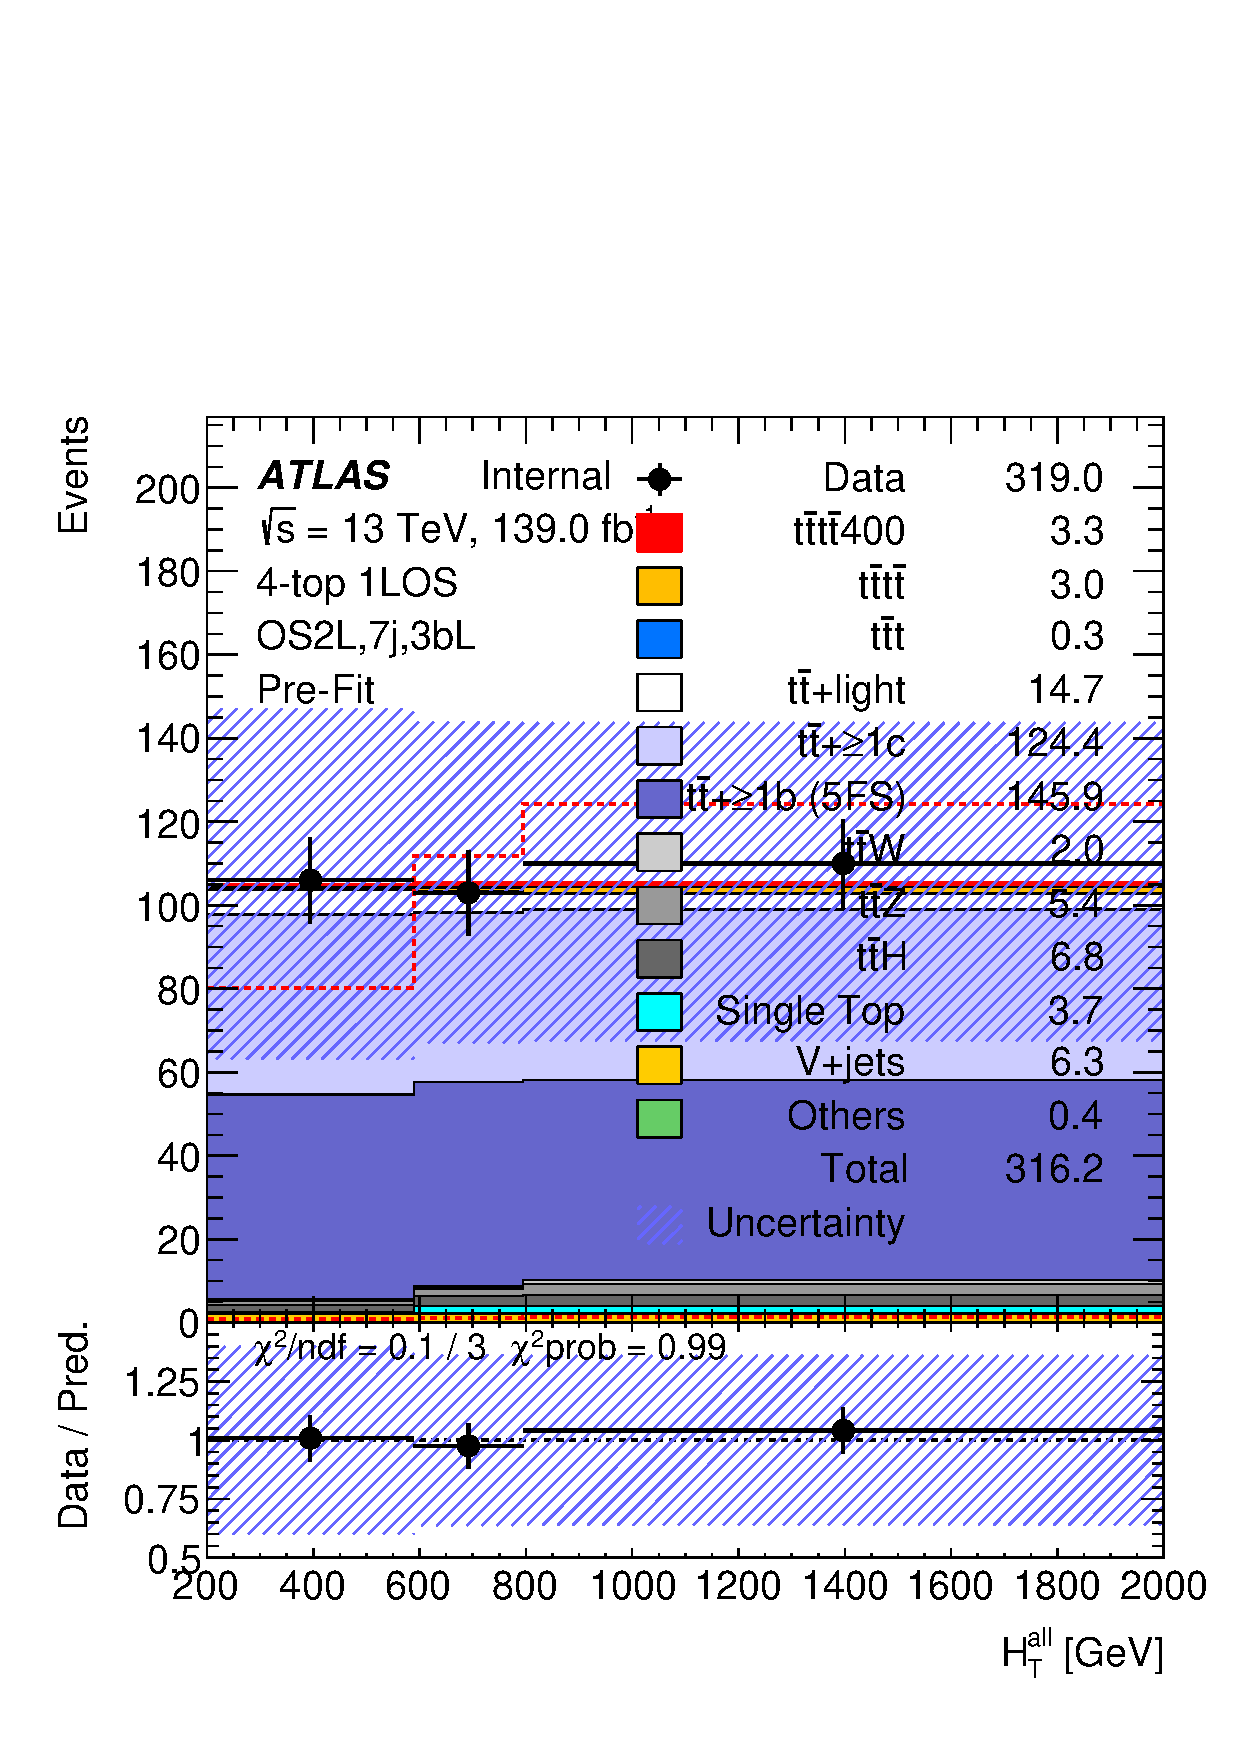
\includegraphics[width=0.31 \textwidth]{figures/fits/GNN/400/2L/data_unblindedSplusB/Plots/os2l_7j3bL.pdf} &
        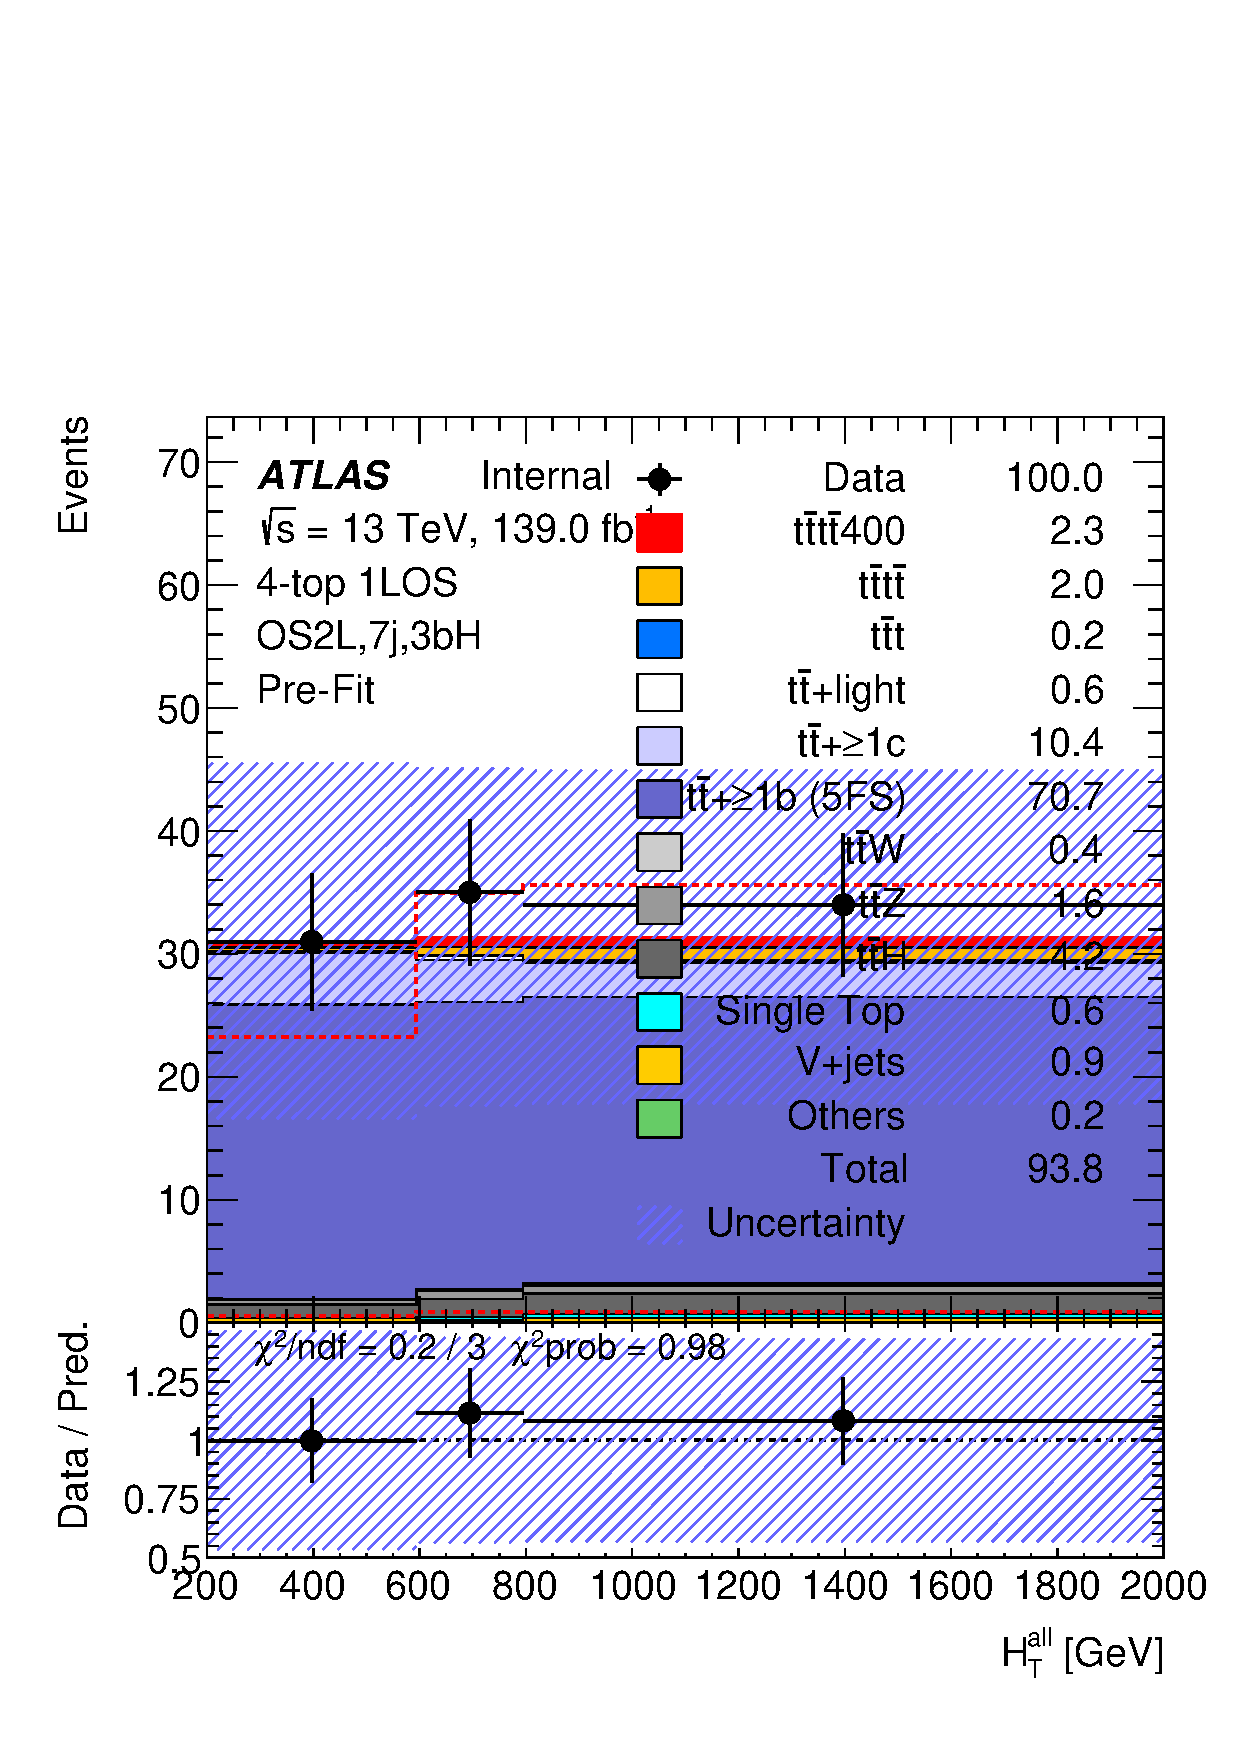
\includegraphics[width=0.31 \textwidth]{figures/fits/GNN/400/2L/data_unblindedSplusB/Plots/os2l_7j3bH.pdf} &
        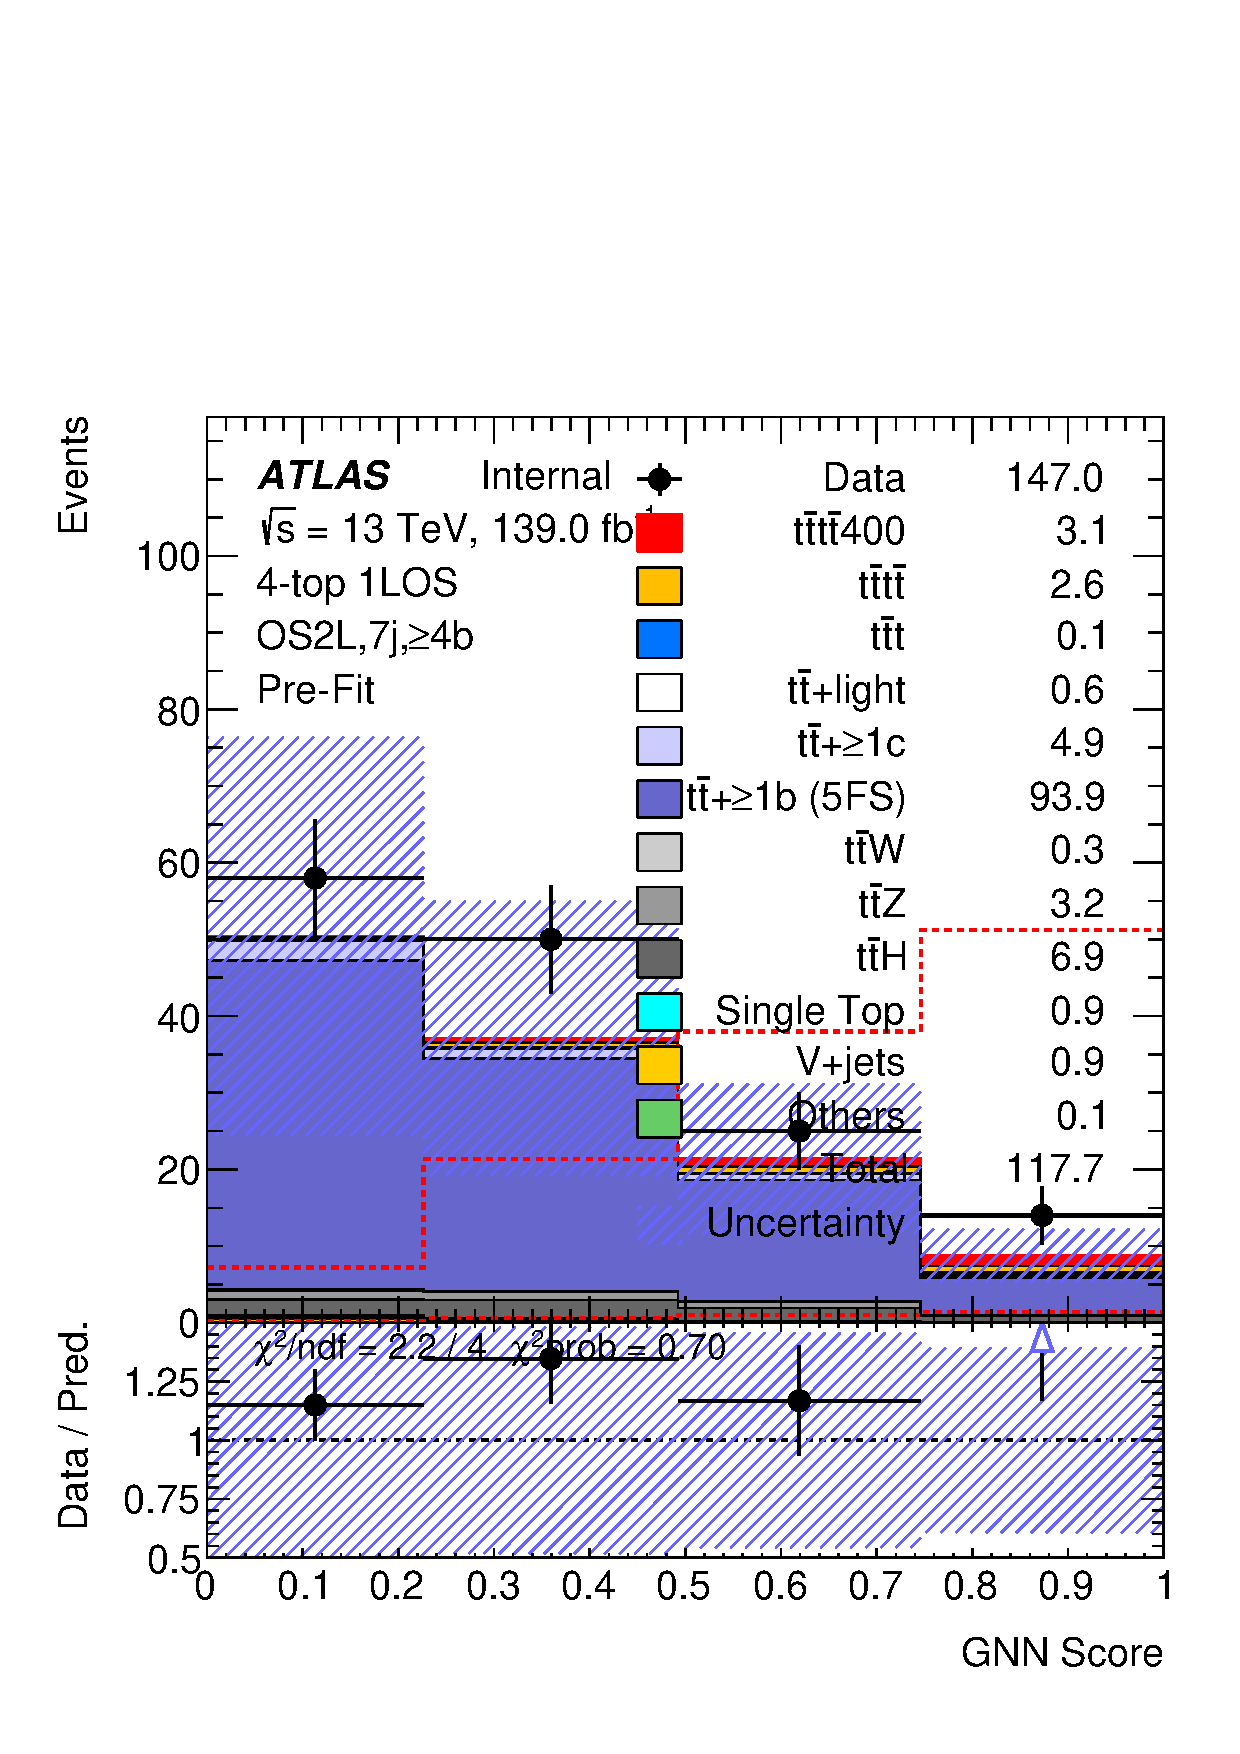
\includegraphics[width=0.31 \textwidth]{figures/fits/GNN/400/2L/data_unblindedSplusB/Plots/os2l_7jge4b.pdf} \\

        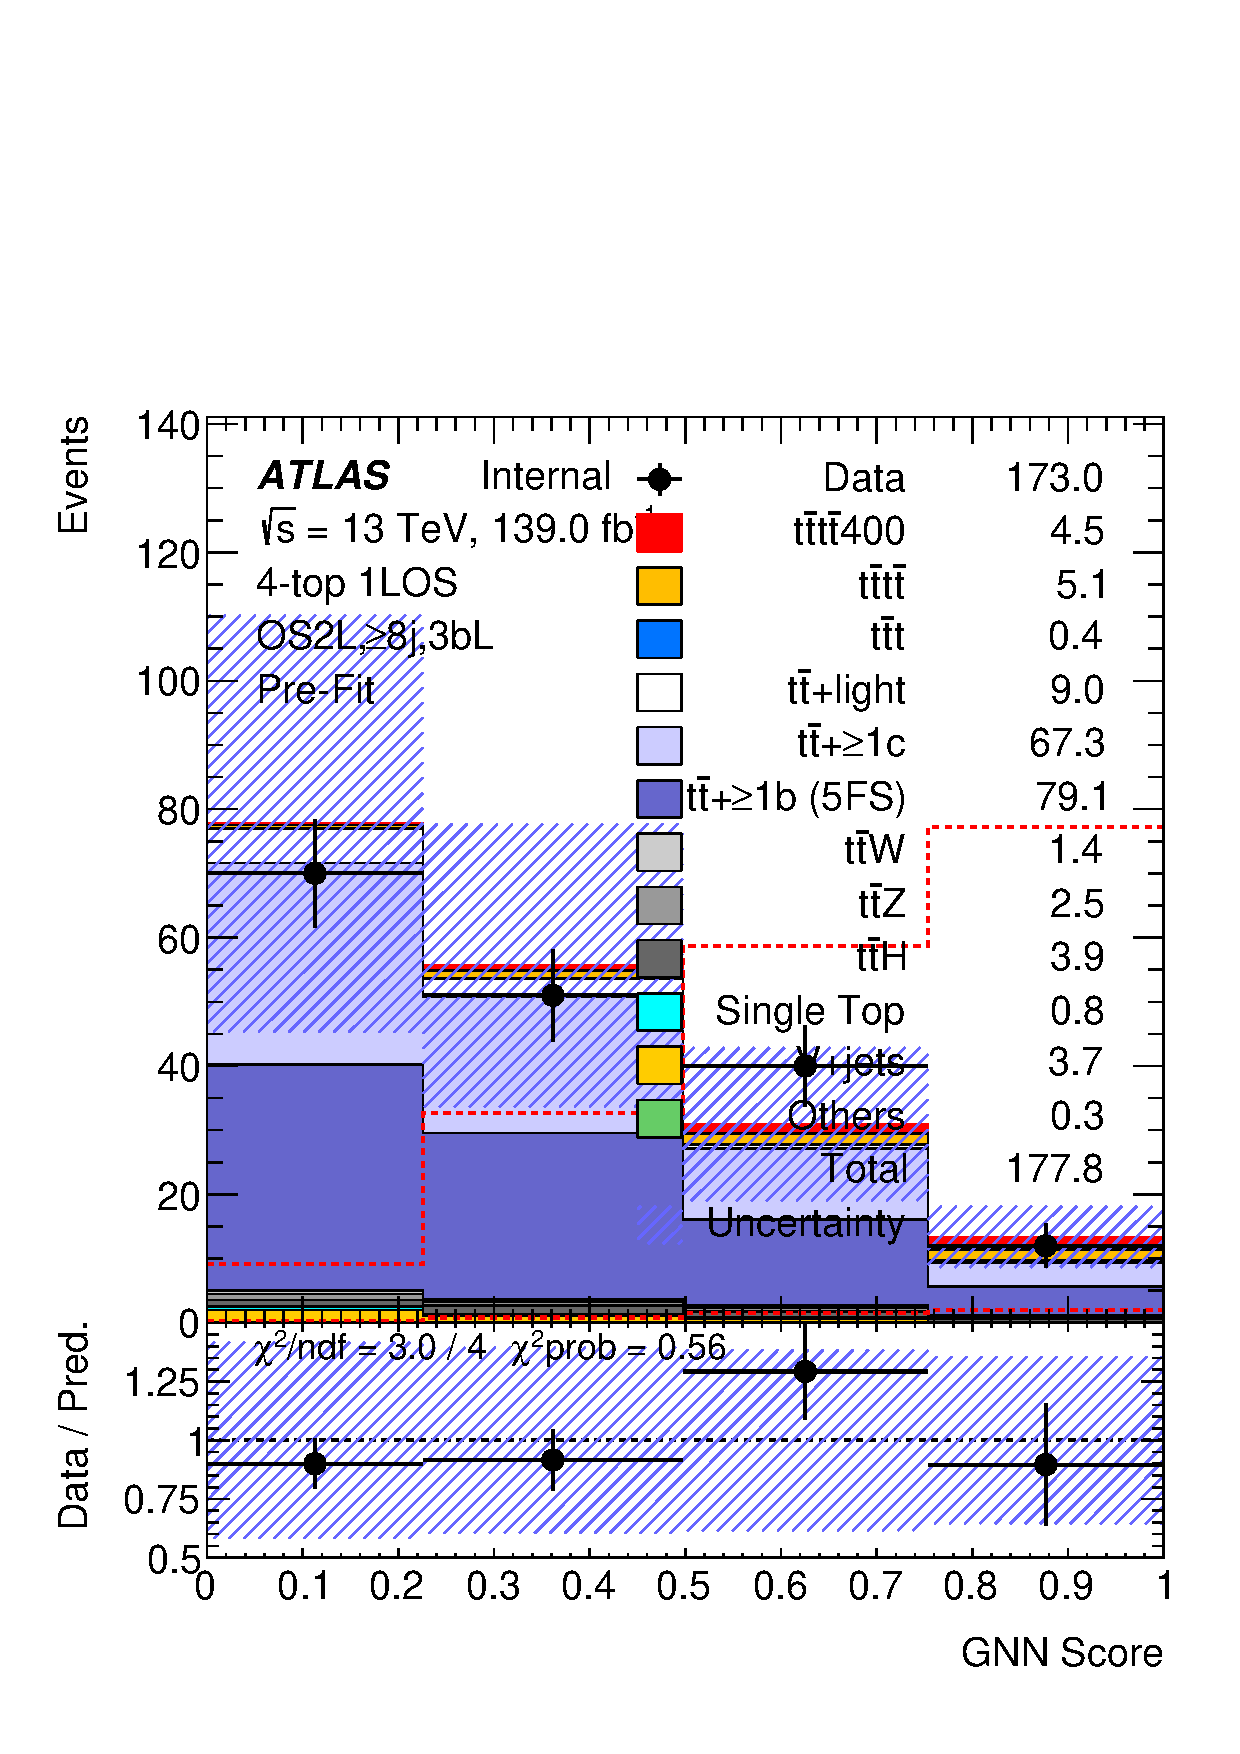
\includegraphics[width=0.31 \textwidth]{figures/fits/GNN/400/2L/data_unblindedSplusB/Plots/os2l_ge8j3bL.pdf} &
        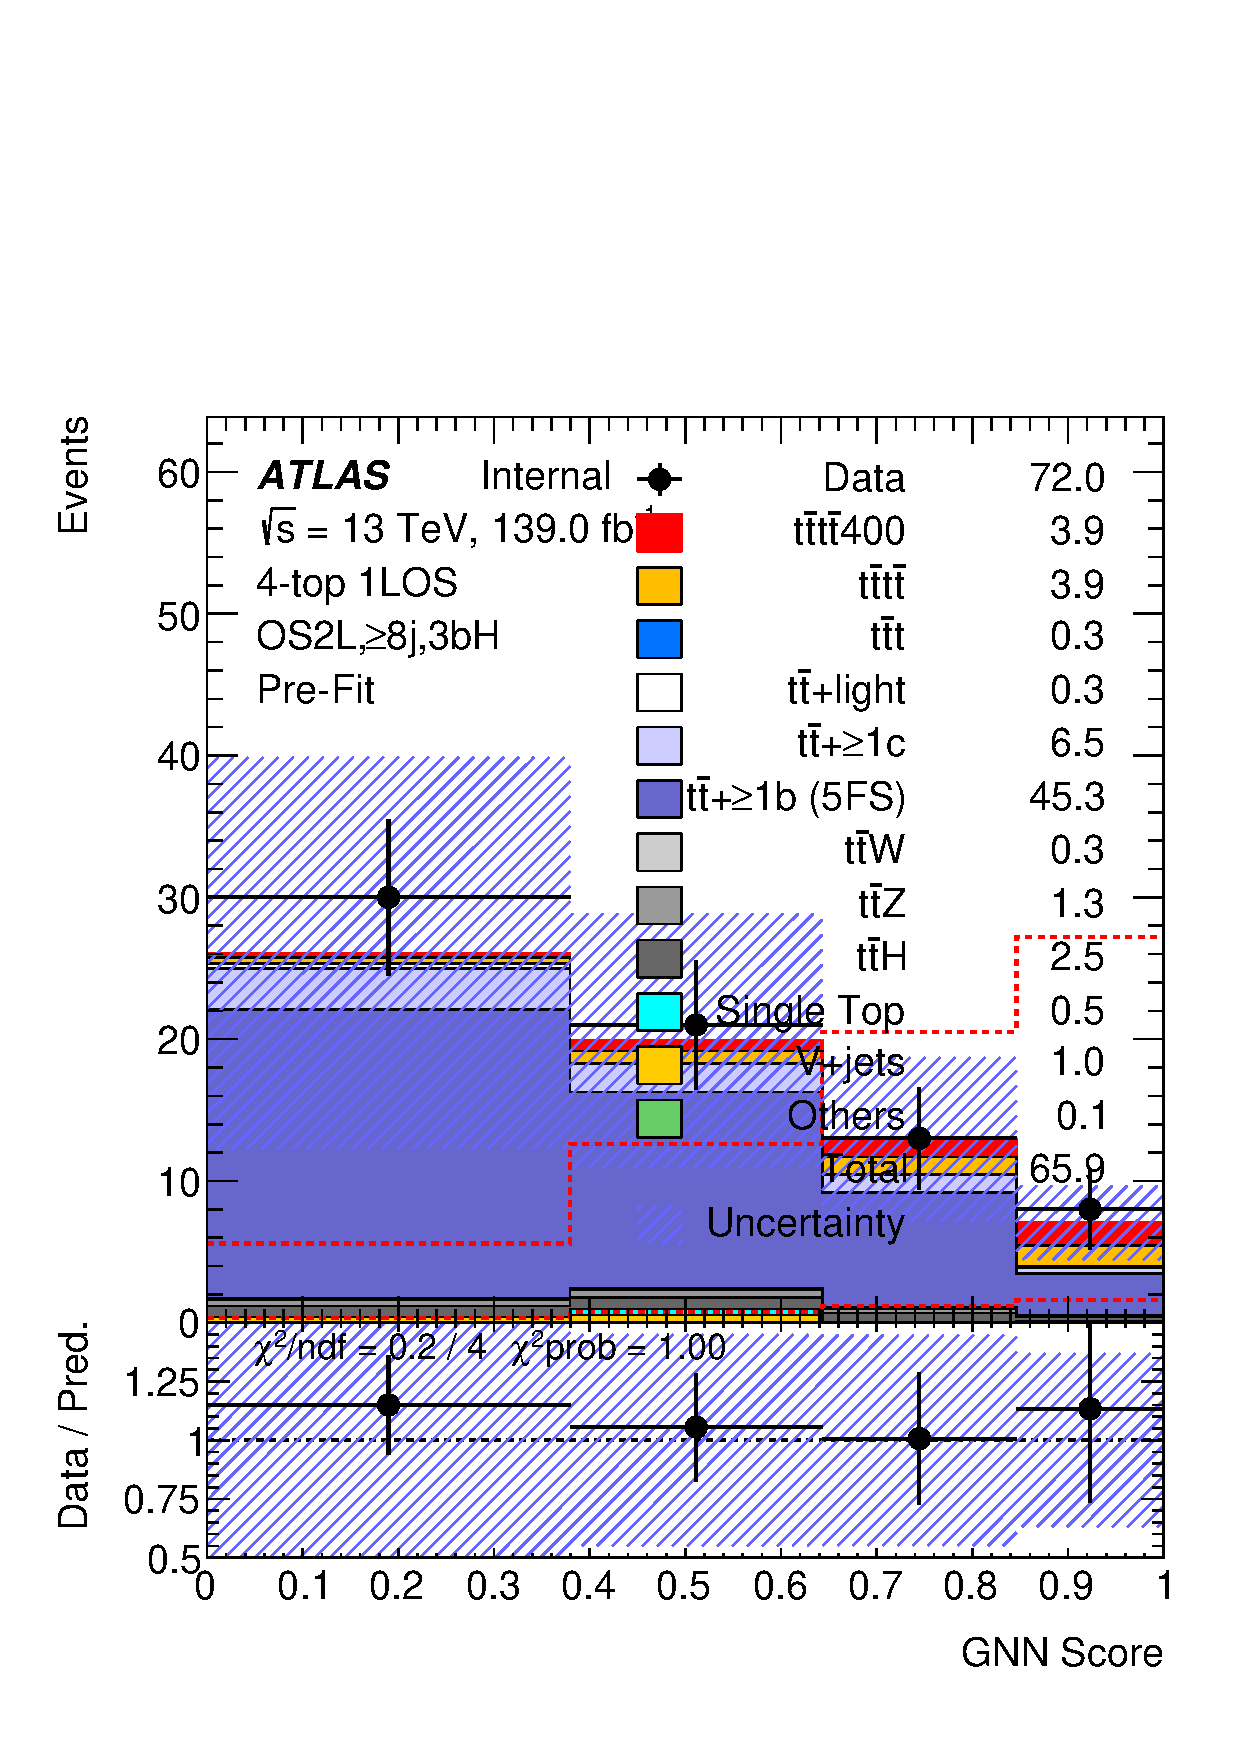
\includegraphics[width=0.31 \textwidth]{figures/fits/GNN/400/2L/data_unblindedSplusB/Plots/os2l_ge8j3bH.pdf} &
        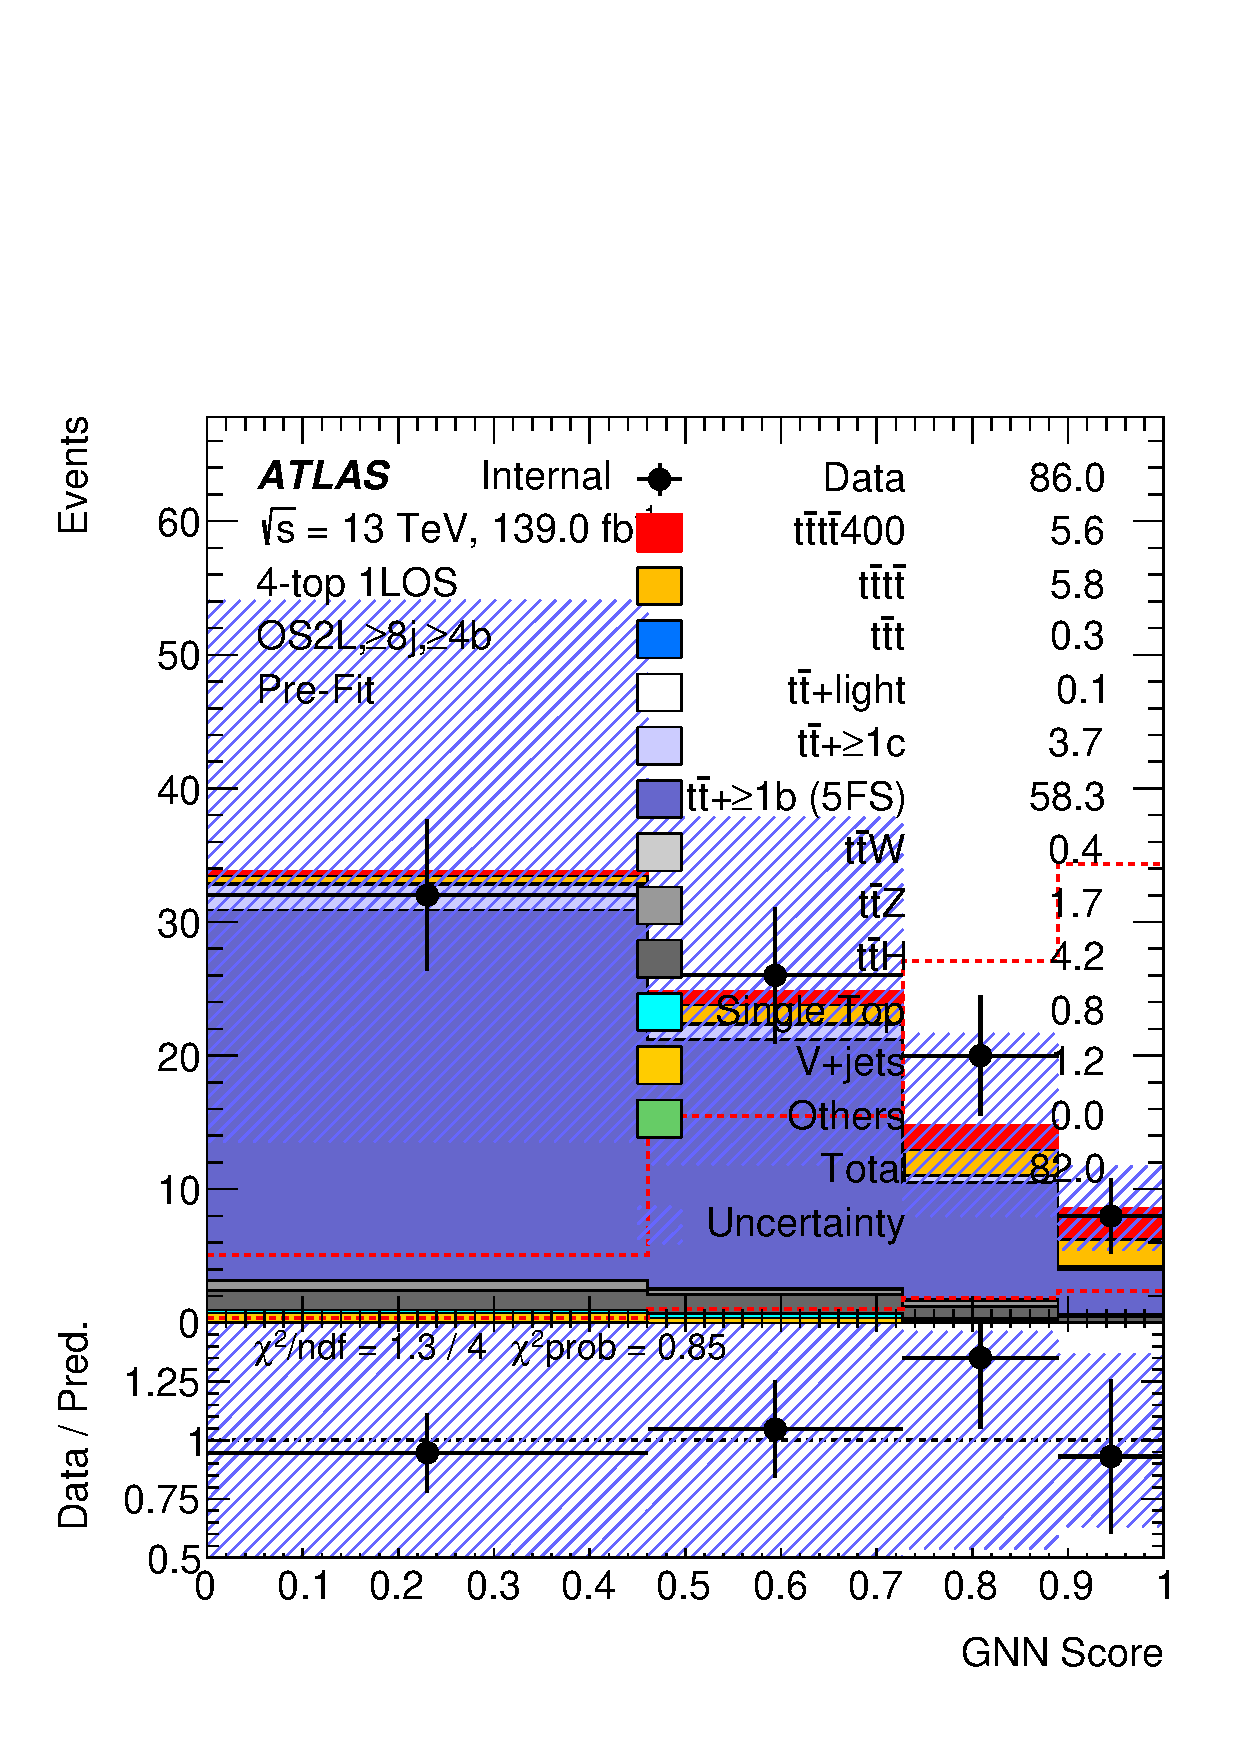
\includegraphics[width=0.31 \textwidth]{figures/fits/GNN/400/2L/data_unblindedSplusB/Plots/os2l_ge8jge4b.pdf} \\
        \end{tabular}
        \caption{\label{fig:Prefit_Yields_2L}Pre-fit distributions for 2LOS channel associated with different signal and background samples, compared with data yields. In general, MC samples and data have good agreement. The signal sample is normalised to a cross-section of 12 fb.}
\end{center}
\end{figure}


\begin{figure}[htbp!]
  \centering
  \begin{subfigure}[t]{0.32\textwidth}
    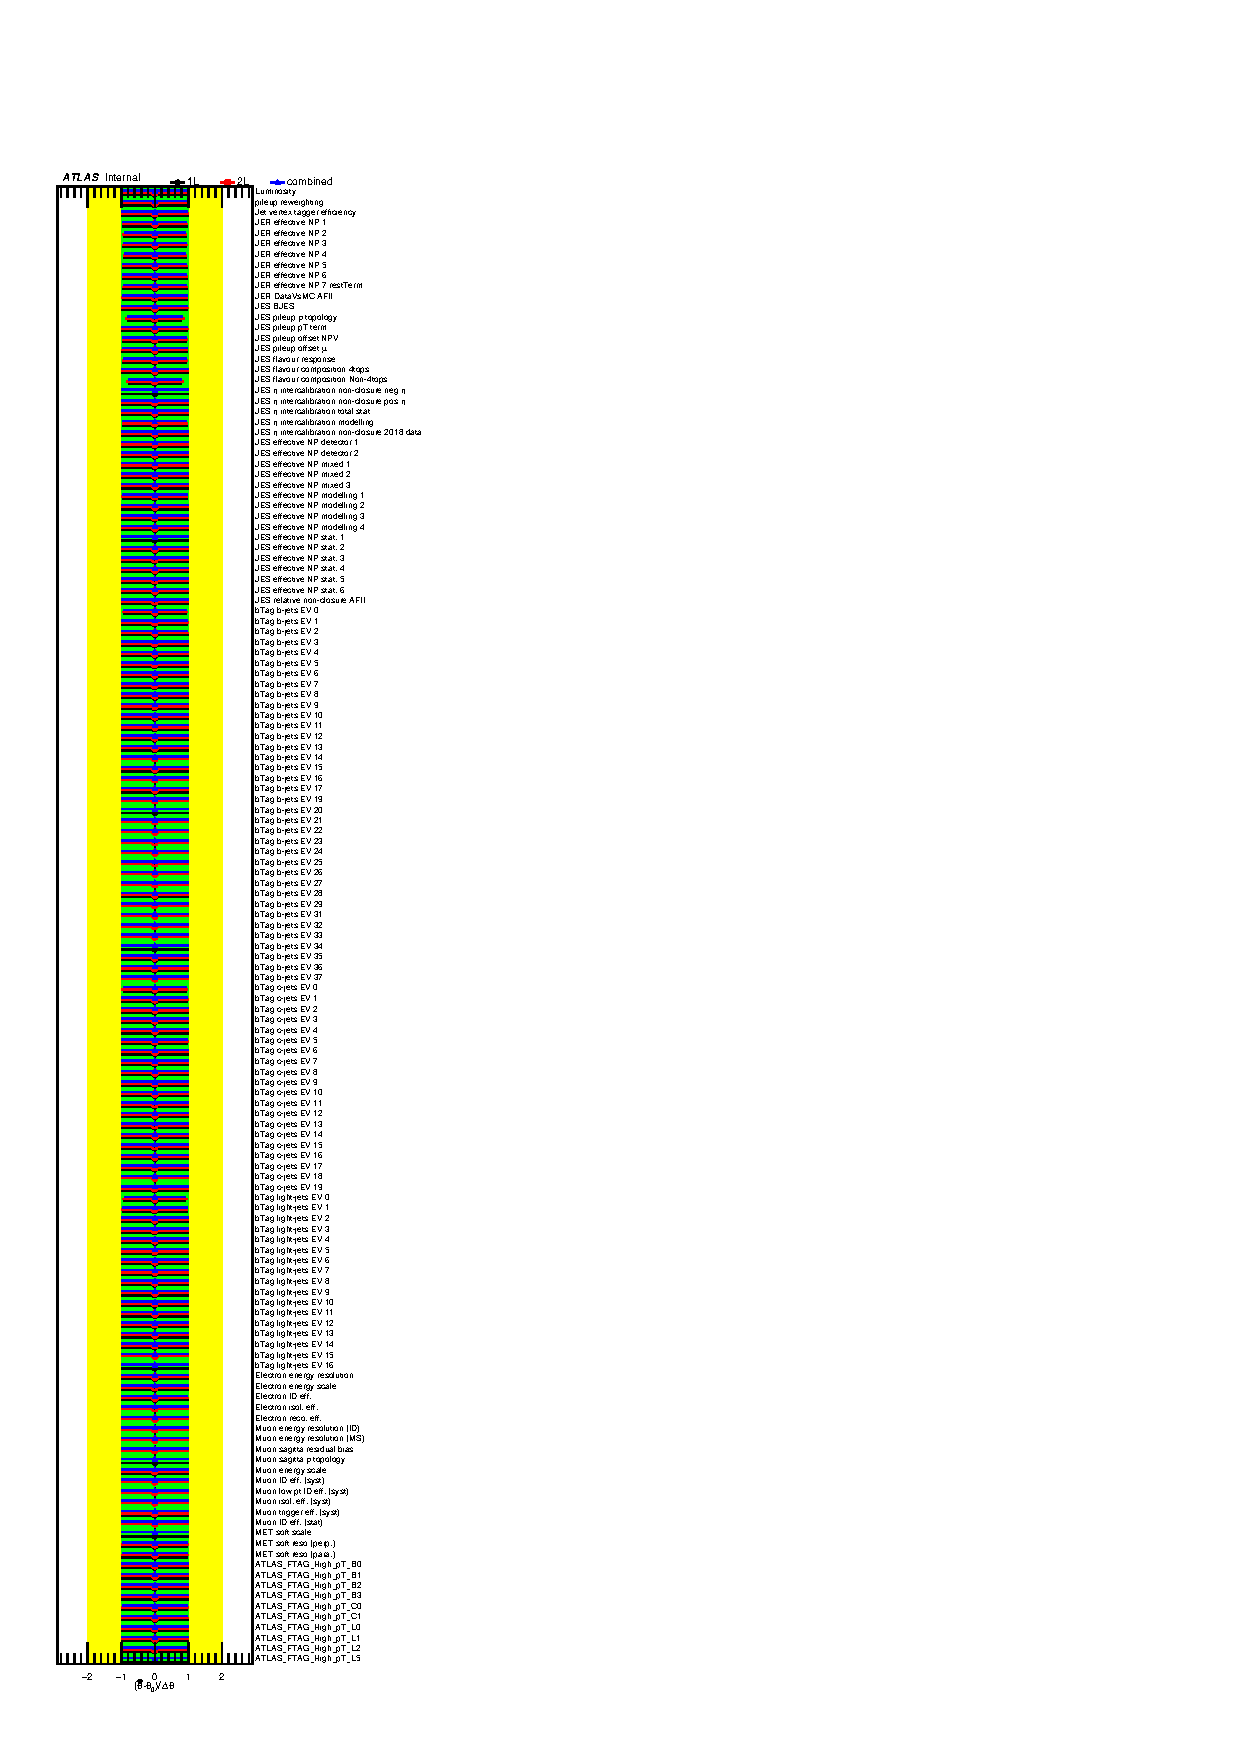
\includegraphics[width=\linewidth]{figures/fits/comparisons/selections/GNN/400/asimov/NuisPar_comp_Instrumental.pdf}
    \subcaption{mH=400\gev}
    \label{fig:Plain_NP_mH40}
  \end{subfigure}
  \begin{subfigure}[t]{0.32\textwidth}
    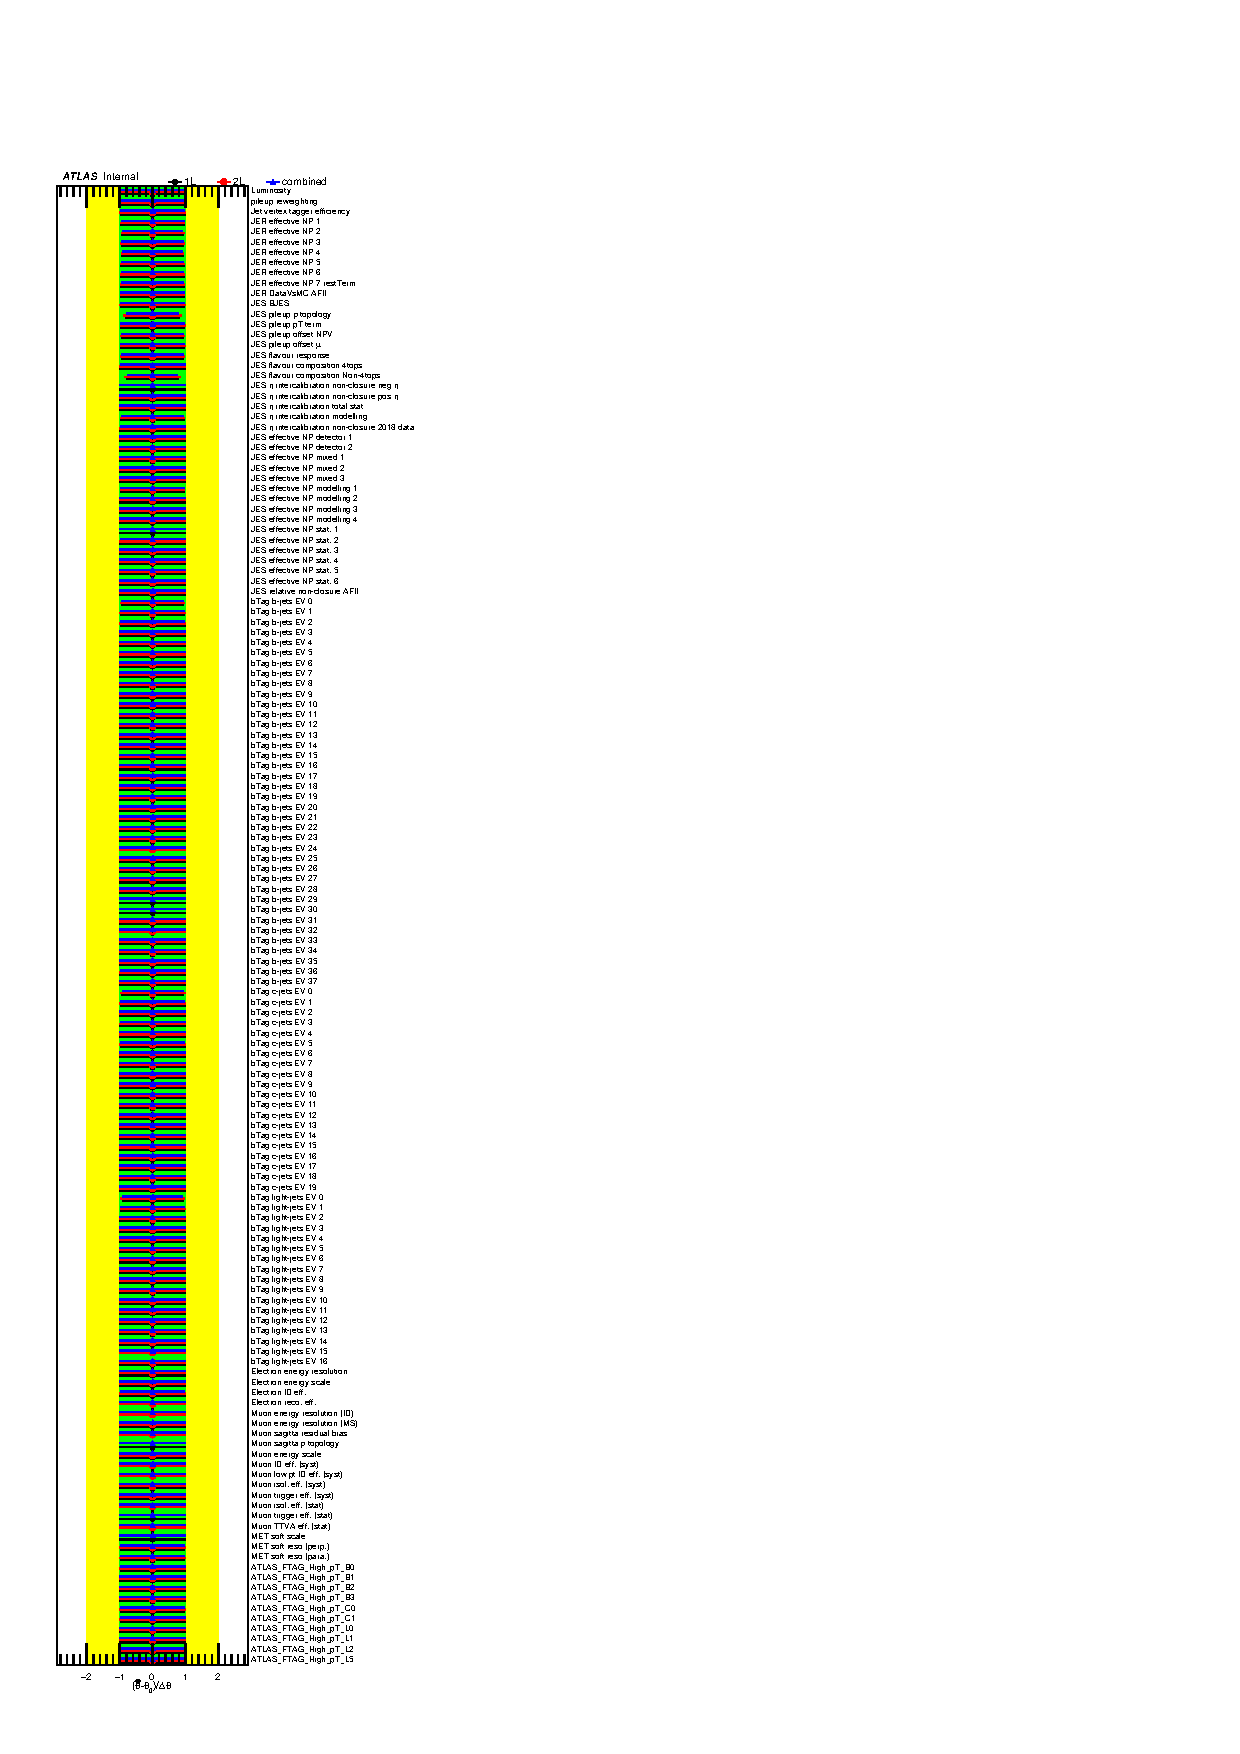
\includegraphics[width=\linewidth]{figures/fits/comparisons/selections/GNN/700/asimov/NuisPar_comp_Instrumental.pdf}
    \subcaption{mH=700\gev}
    \label{fig:Plain_NP_mH40}
  \end{subfigure}
  \begin{subfigure}[t]{0.32\textwidth}
    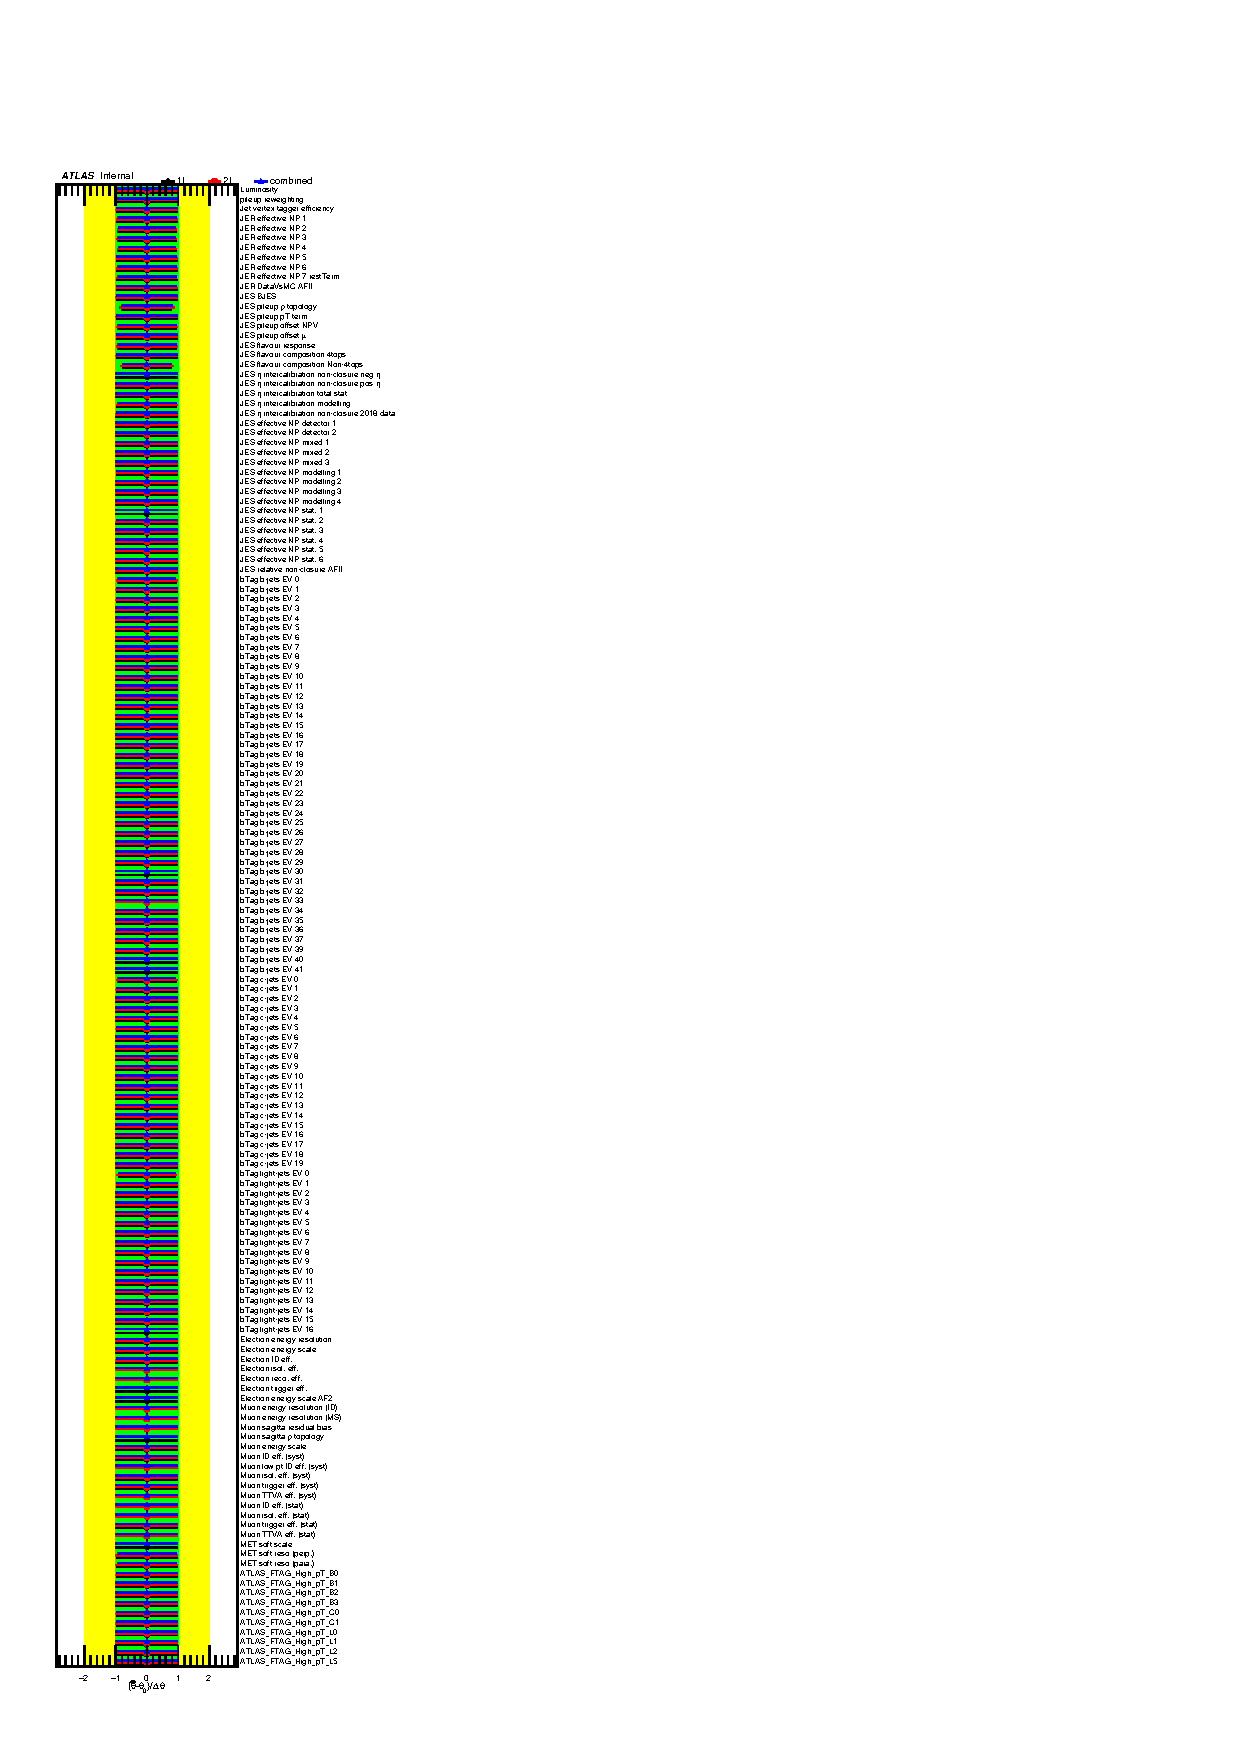
\includegraphics[width=\linewidth]{figures/fits/comparisons/selections/GNN/1000/asimov/NuisPar_comp_Instrumental.pdf}
    \subcaption{mH=1000\gev}
    \label{fig:Plain_NP_mH40}
  \end{subfigure}
  \caption{\label{fig:Plain_NP_instrumental}Fitted pulls and constraints for the nuisance parameters corresponding to the instrumental systematic uncertainties for the Plain Asimov fit for three mass points. Comparison is done for three fits: using only 1L regions, using only 2LOS regions and using all regions.}
\end{figure}


\begin{figure}[htbp!]
  \centering
  \begin{subfigure}[t]{0.32\textwidth}
    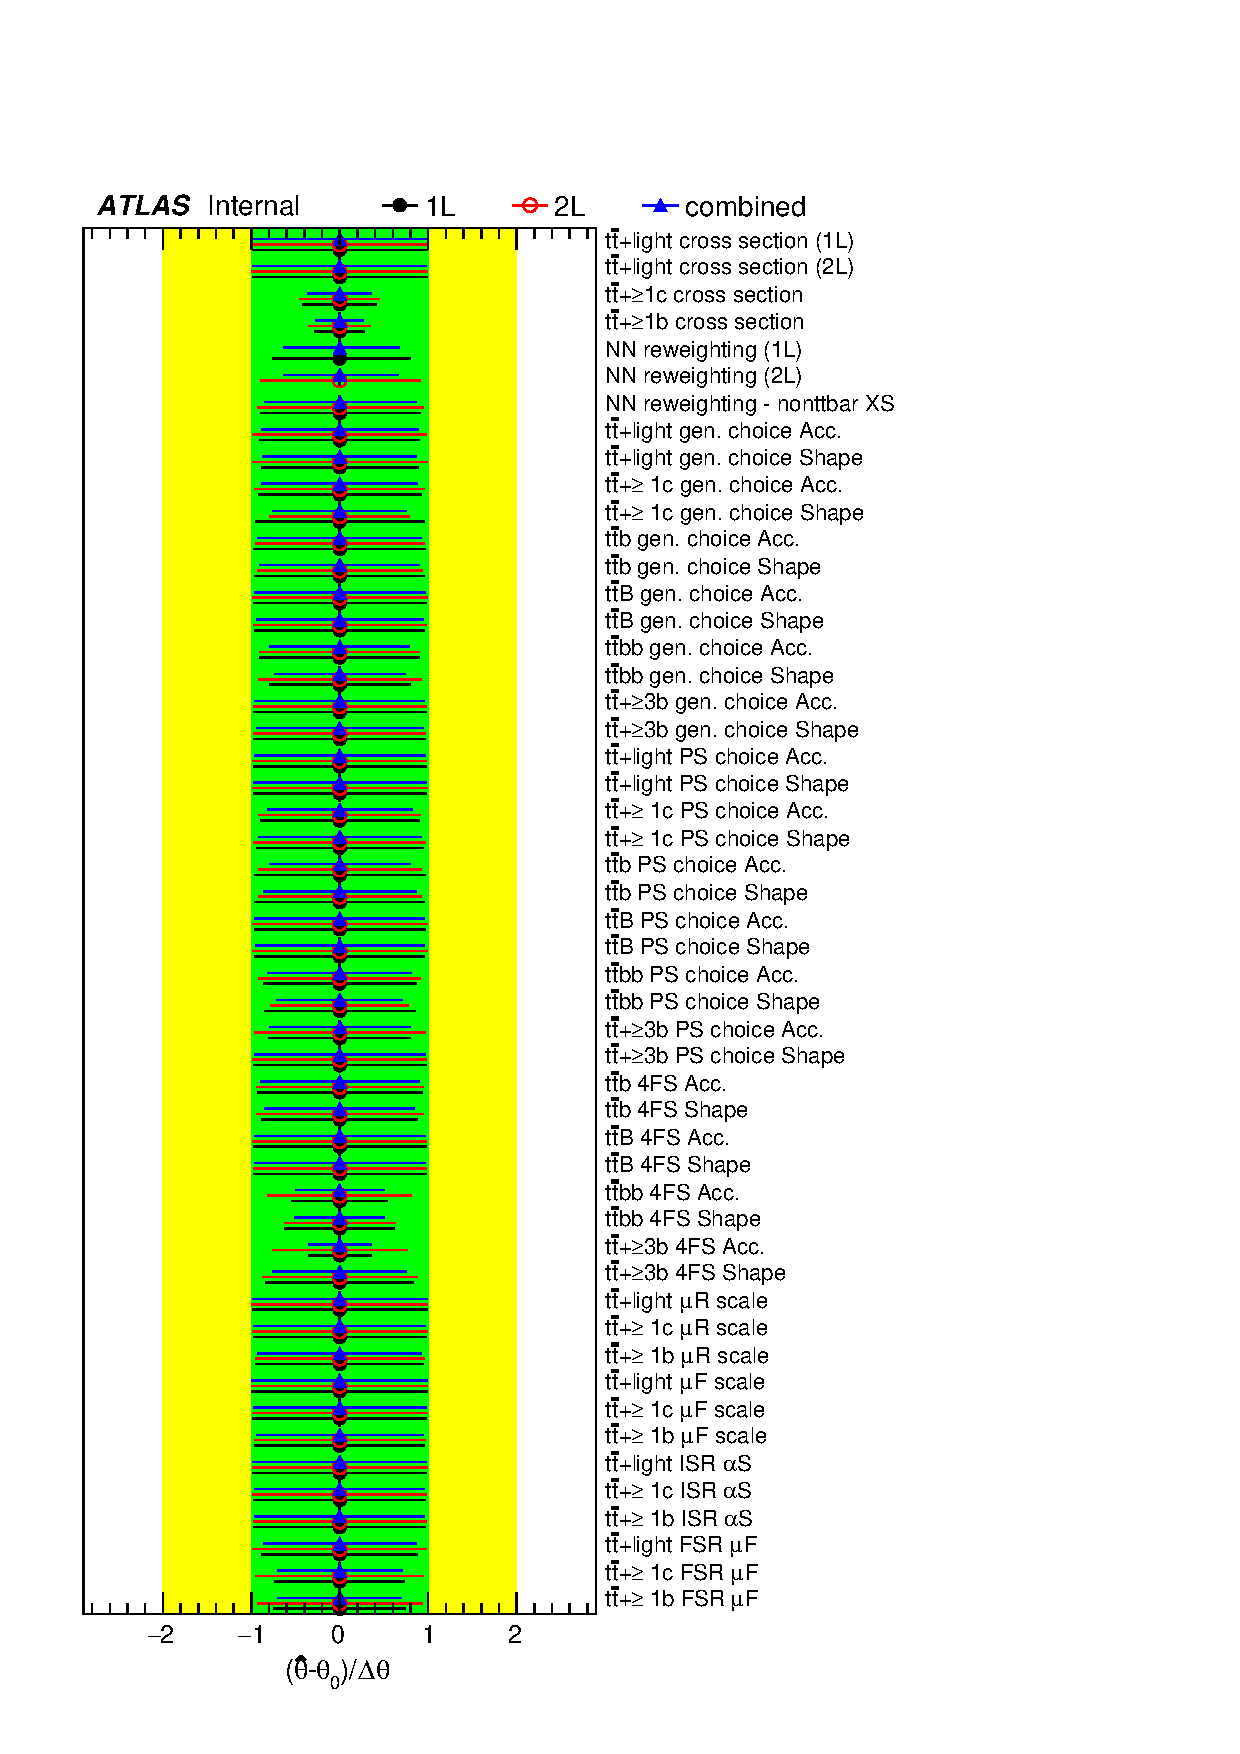
\includegraphics[width=\linewidth]{figures/fits/comparisons/selections/GNN/400/asimov/NuisPar_comp_ttbar.pdf}
    \subcaption{mH=400\gev}
    \label{fig:Plain_NP_mH40}
  \end{subfigure}
  \begin{subfigure}[t]{0.32\textwidth}
    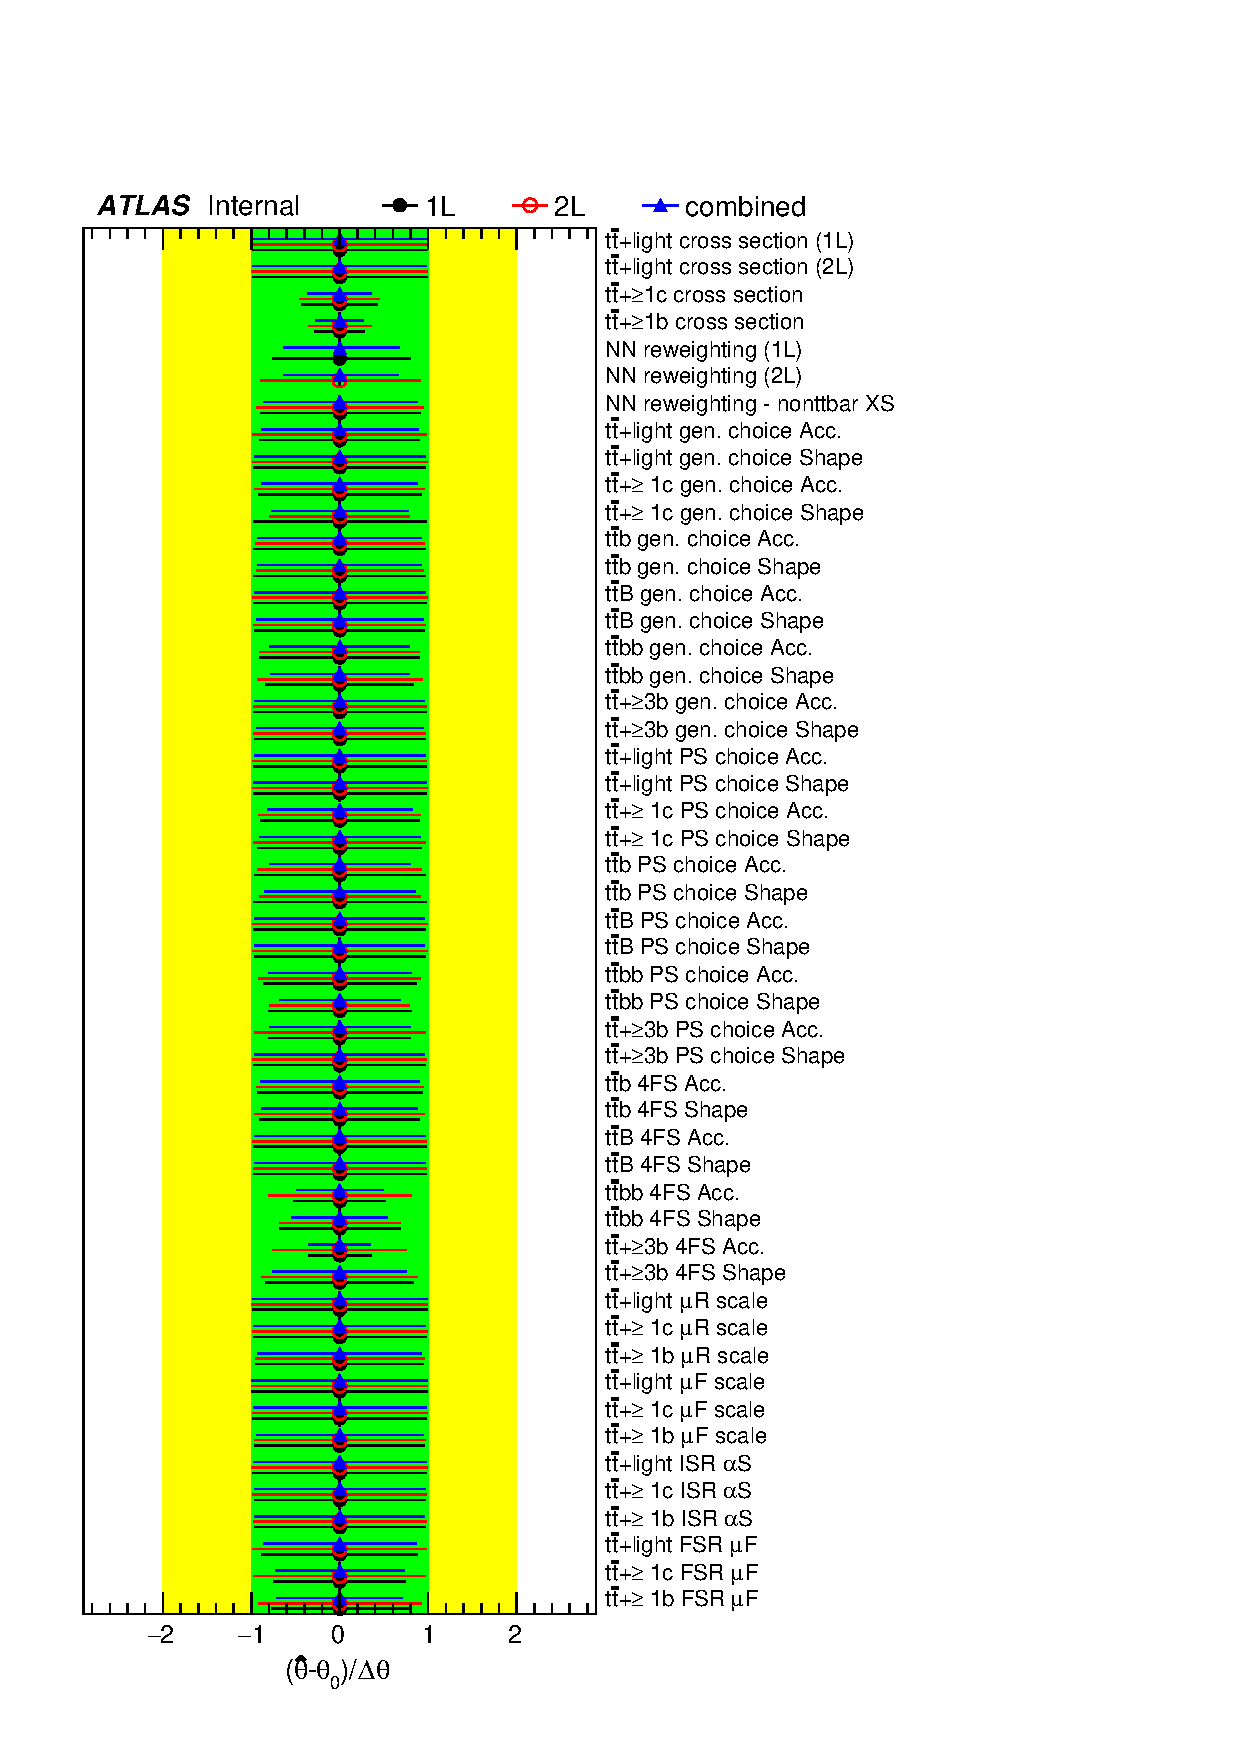
\includegraphics[width=\linewidth]{figures/fits/comparisons/selections/GNN/700/asimov/NuisPar_comp_ttbar.pdf}
    \subcaption{mH=700\gev}
    \label{fig:Plain_NP_mH40}
  \end{subfigure}
  \begin{subfigure}[t]{0.32\textwidth}
    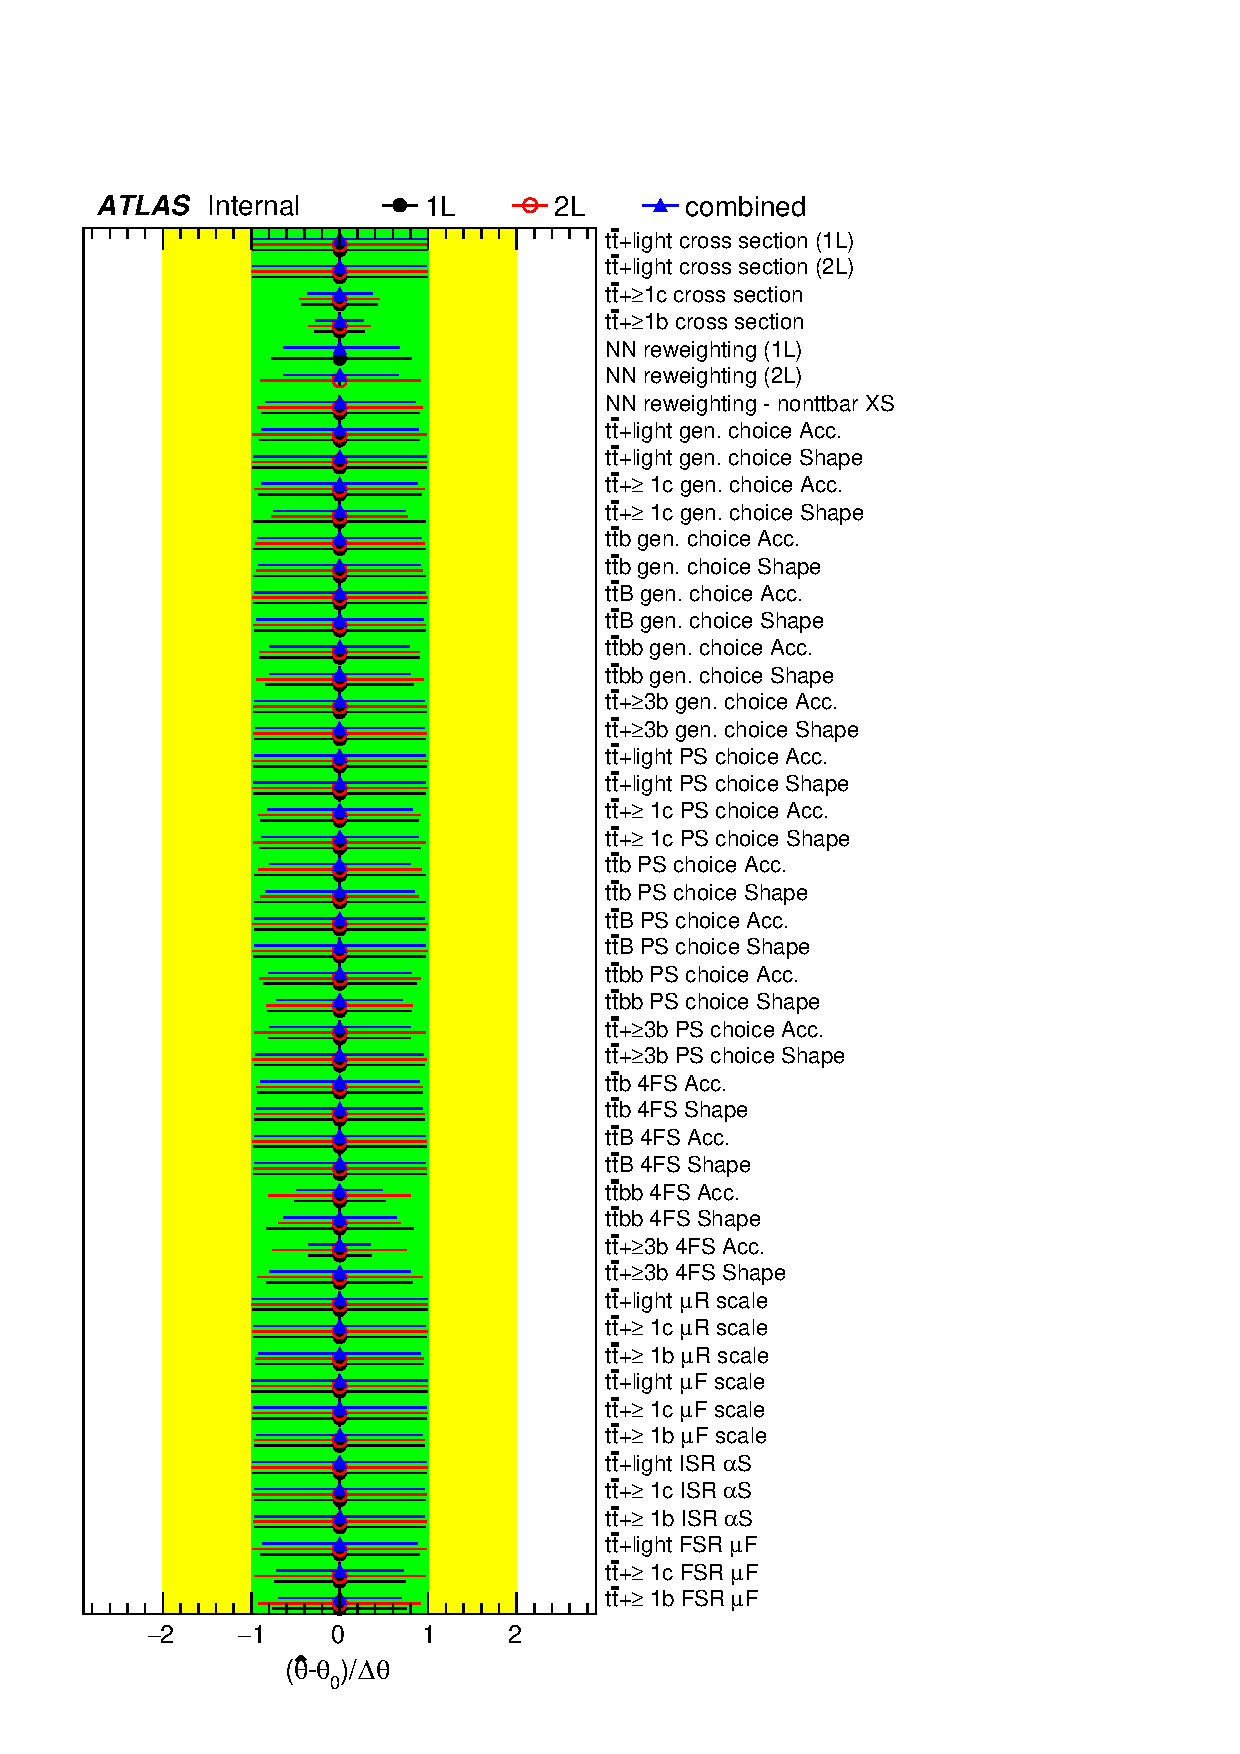
\includegraphics[width=\linewidth]{figures/fits/comparisons/selections/GNN/1000/asimov/NuisPar_comp_ttbar.pdf}
    \subcaption{mH=1000\gev}
    \label{fig:Plain_NP_mH40}
  \end{subfigure}
  \caption{\label{fig:Plain_NP_ttbar}Fitted pulls and constraints for the nuisance parameters corresponding to the \ttbar systematic uncertainties for the Plain Asimov fit for three mass points. Comparison is done for three fits: using only 1L regions, using only 2LOS regions and using all regions.}
\end{figure}


\begin{figure}[htbp!]
  \centering
  \begin{subfigure}[t]{0.32\textwidth}
    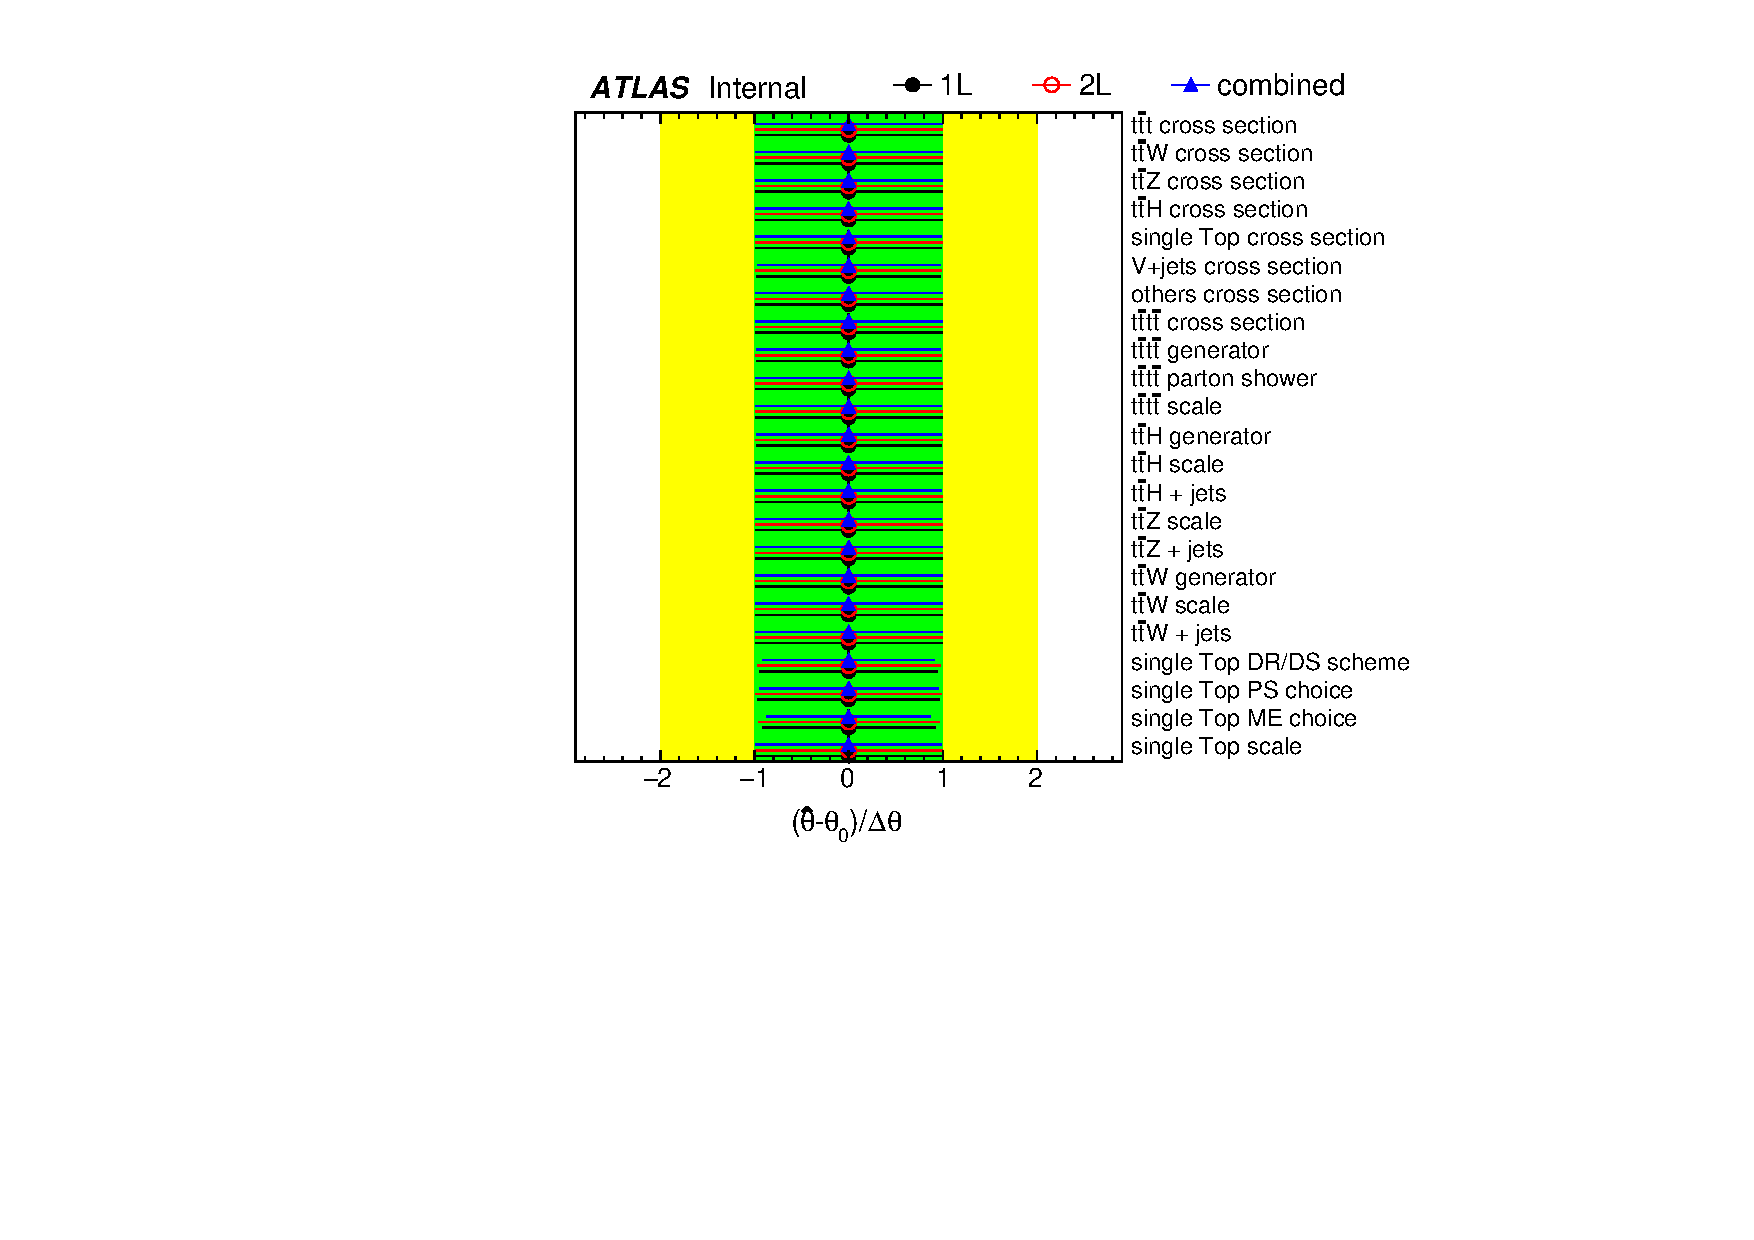
\includegraphics[width=\linewidth]{figures/fits/comparisons/selections/GNN/400/asimov/NuisPar_comp_Other.pdf}
    \subcaption{mH=400\gev}
    \label{fig:Plain_NP_mH40}
  \end{subfigure}
  \begin{subfigure}[t]{0.32\textwidth}
    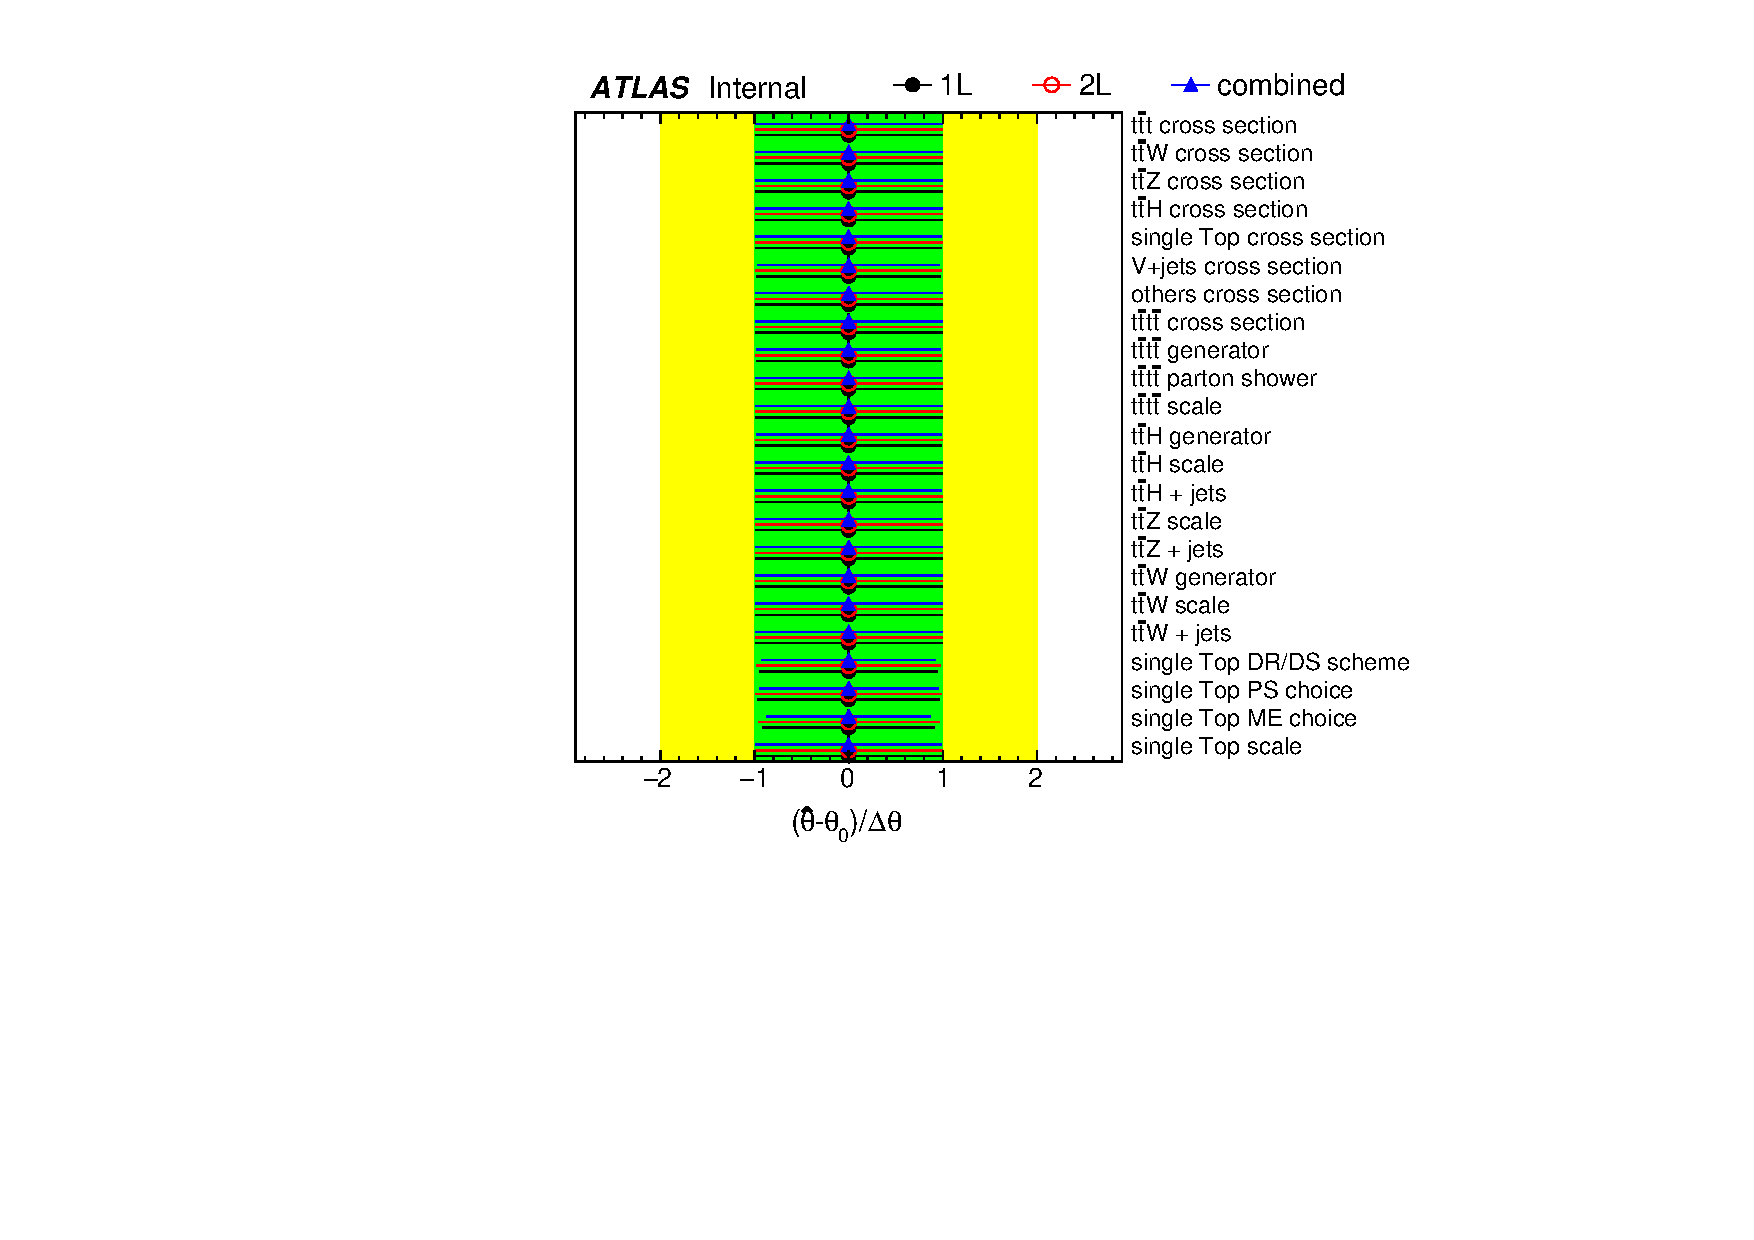
\includegraphics[width=\linewidth]{figures/fits/comparisons/selections/GNN/700/asimov/NuisPar_comp_Other.pdf}
    \subcaption{mH=700\gev}
    \label{fig:Plain_NP_mH40}
  \end{subfigure}
  \begin{subfigure}[t]{0.32\textwidth}
    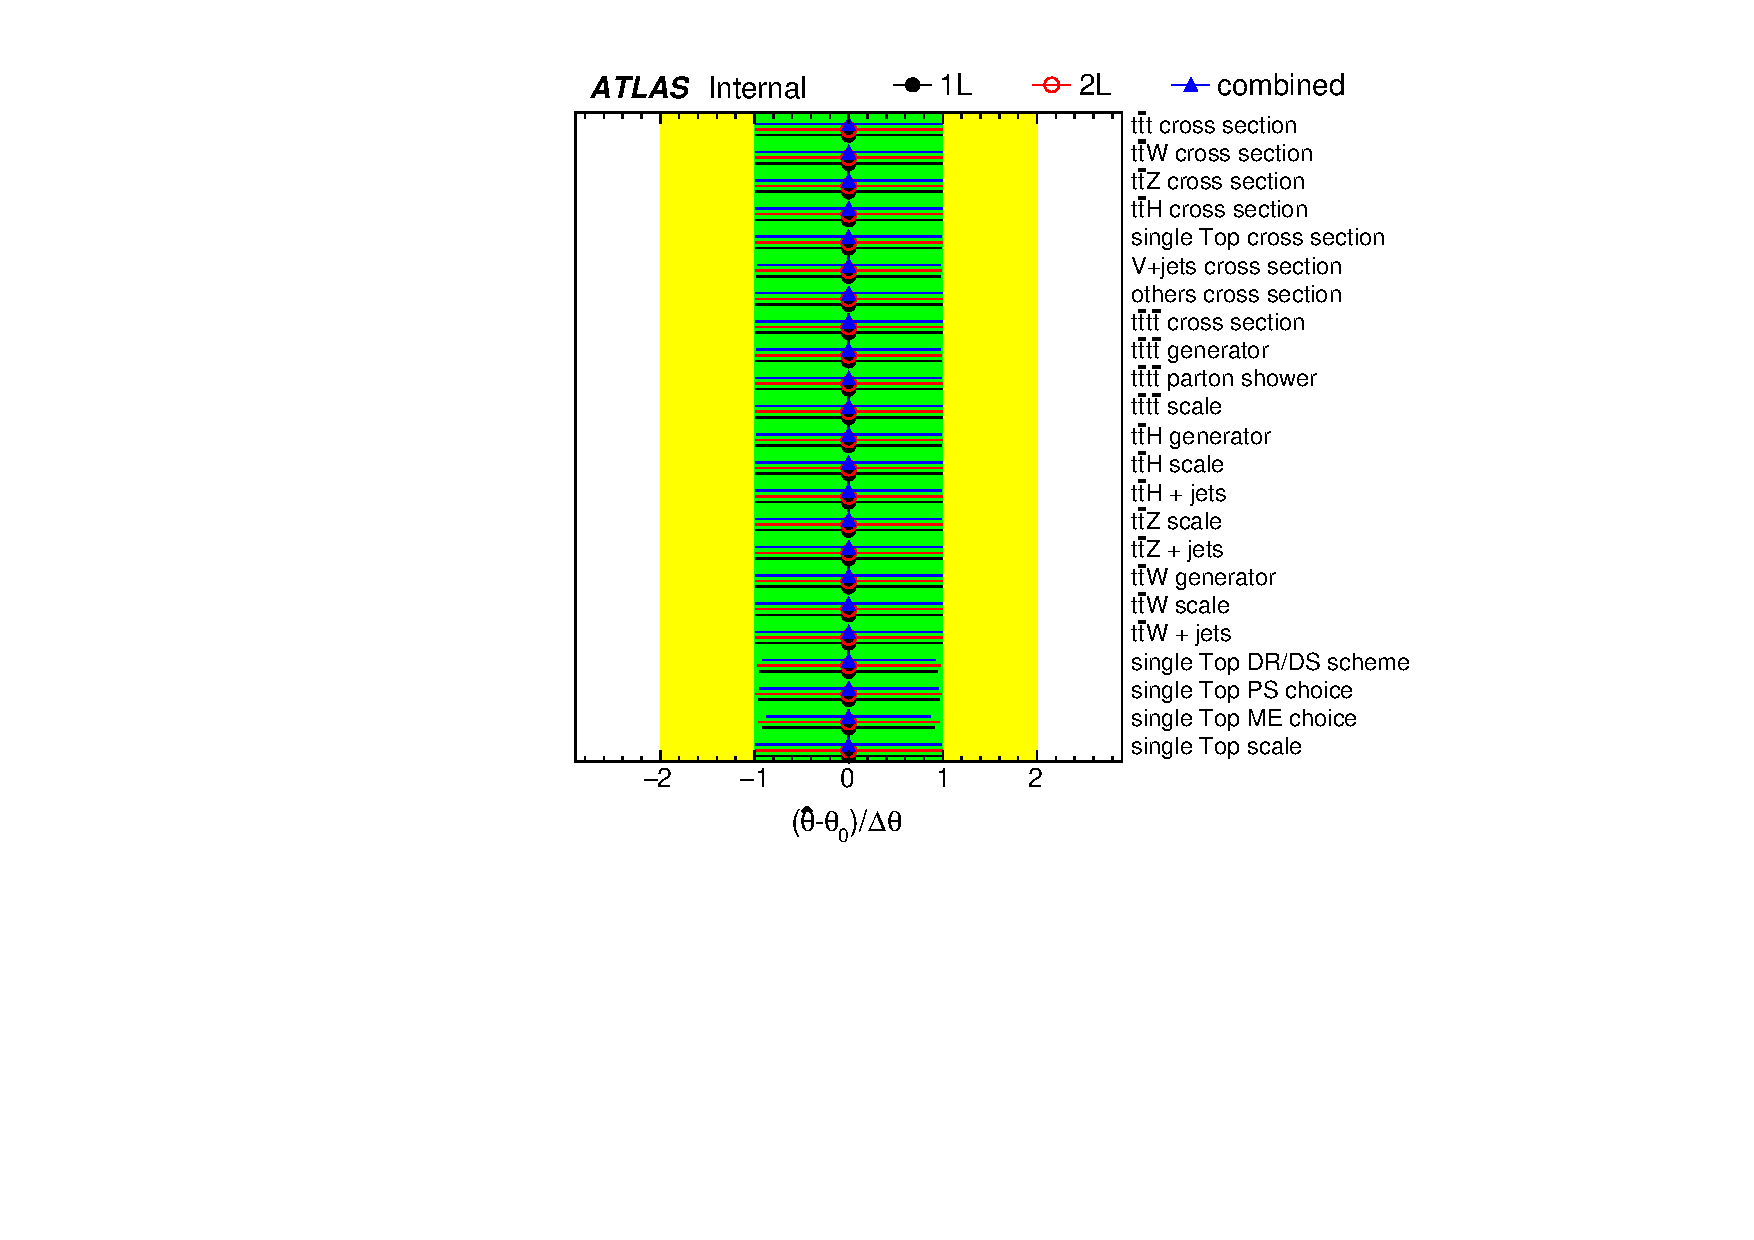
\includegraphics[width=\linewidth]{figures/fits/comparisons/selections/GNN/1000/asimov/NuisPar_comp_Other.pdf}
    \subcaption{mH=1000\gev}
    \label{fig:Plain_NP_mH40}
  \end{subfigure}
  \caption{\label{fig:Plain_NP_other}Fitted pulls and constraints for the nuisance parameters corresponding to the non-\ttbar background systematic uncertainties for the Plain Asimov fit for three mass points. Comparison is done for three fits: using only 1L regions, using only 2LOS regions and using all regions.}
\end{figure}

\begin{figure}[htbp!]
  \centering
  \begin{subfigure}[t]{0.32\textwidth}
    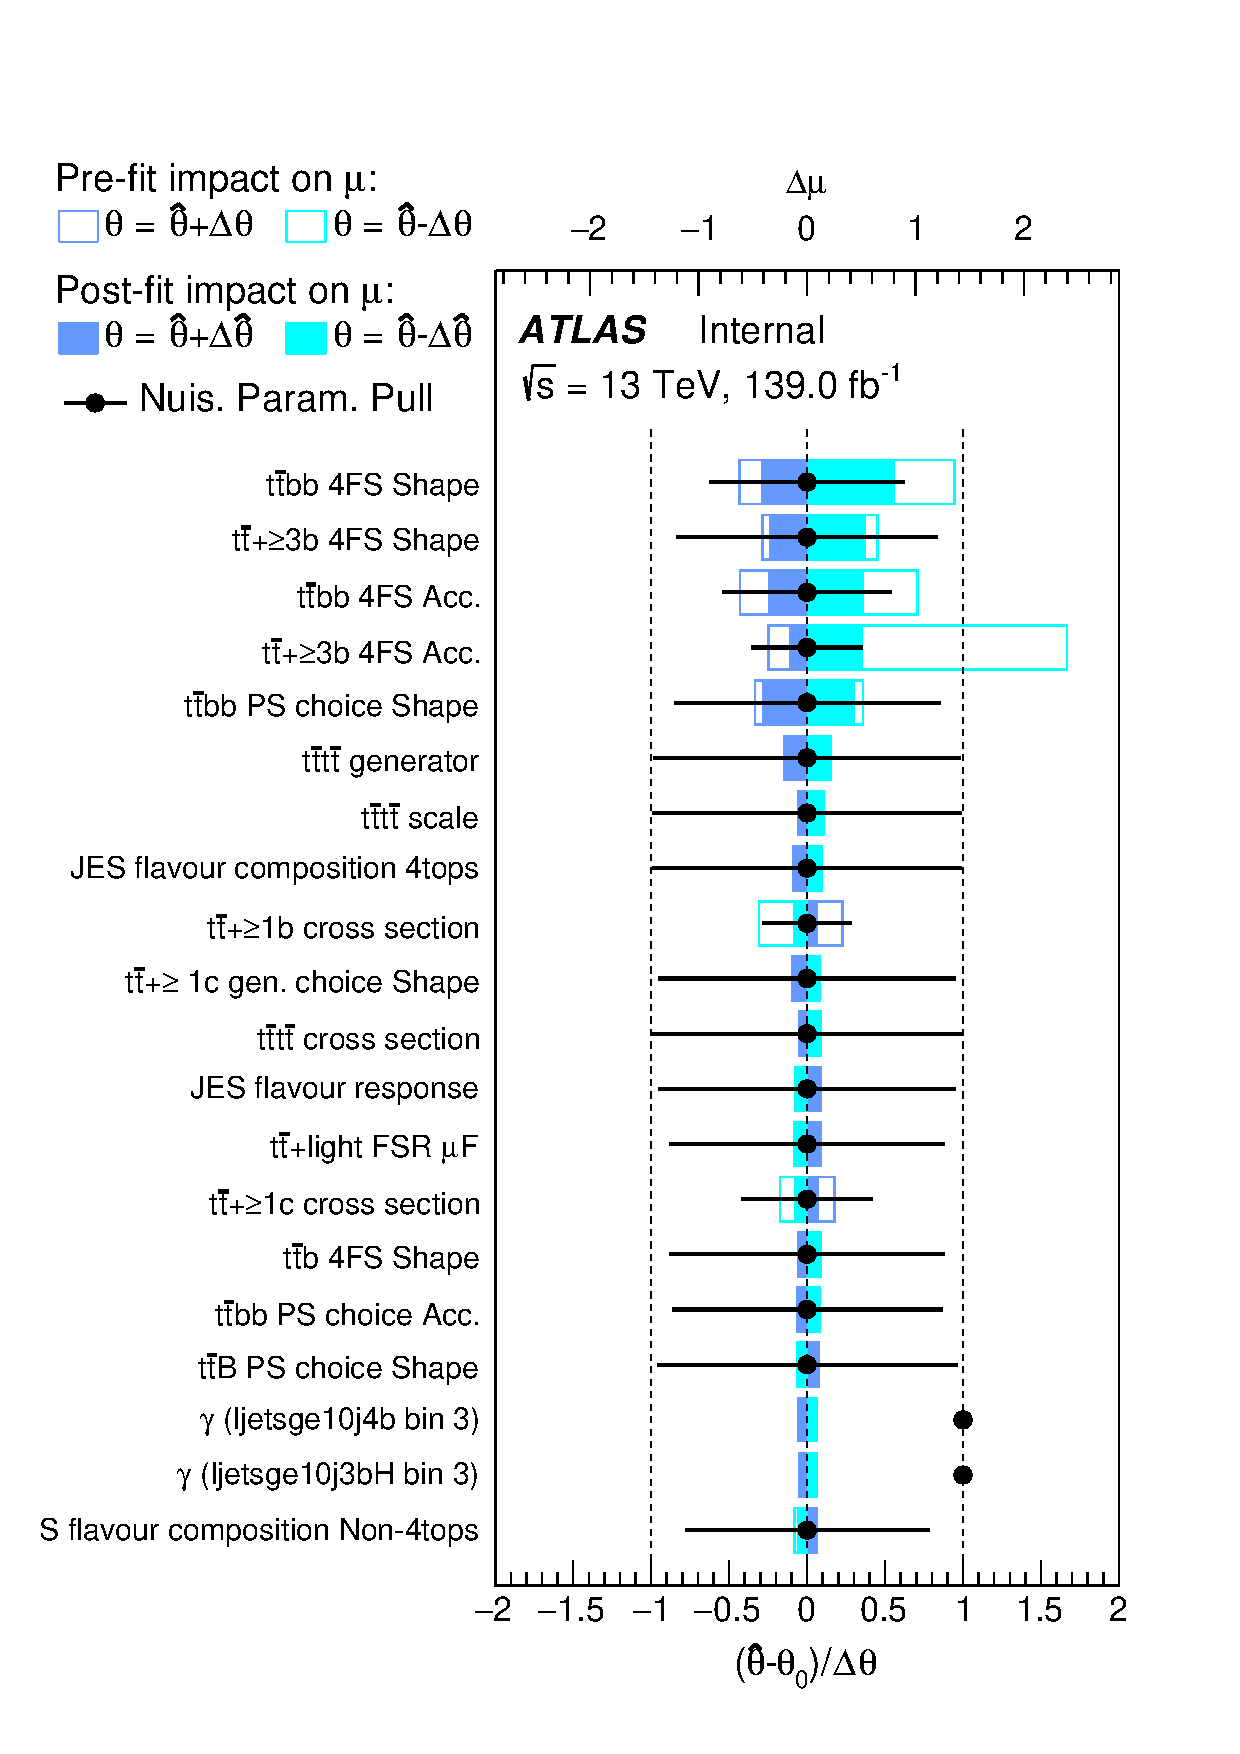
\includegraphics[width=\linewidth]{figures/fits/GNN/400/1L/asimov/Ranking_mu_tttt.pdf}
     \caption{\label{fig:Ranking_mH400_Asimov_1L}1L }
  \end{subfigure}
  \begin{subfigure}[t]{0.32\textwidth}
    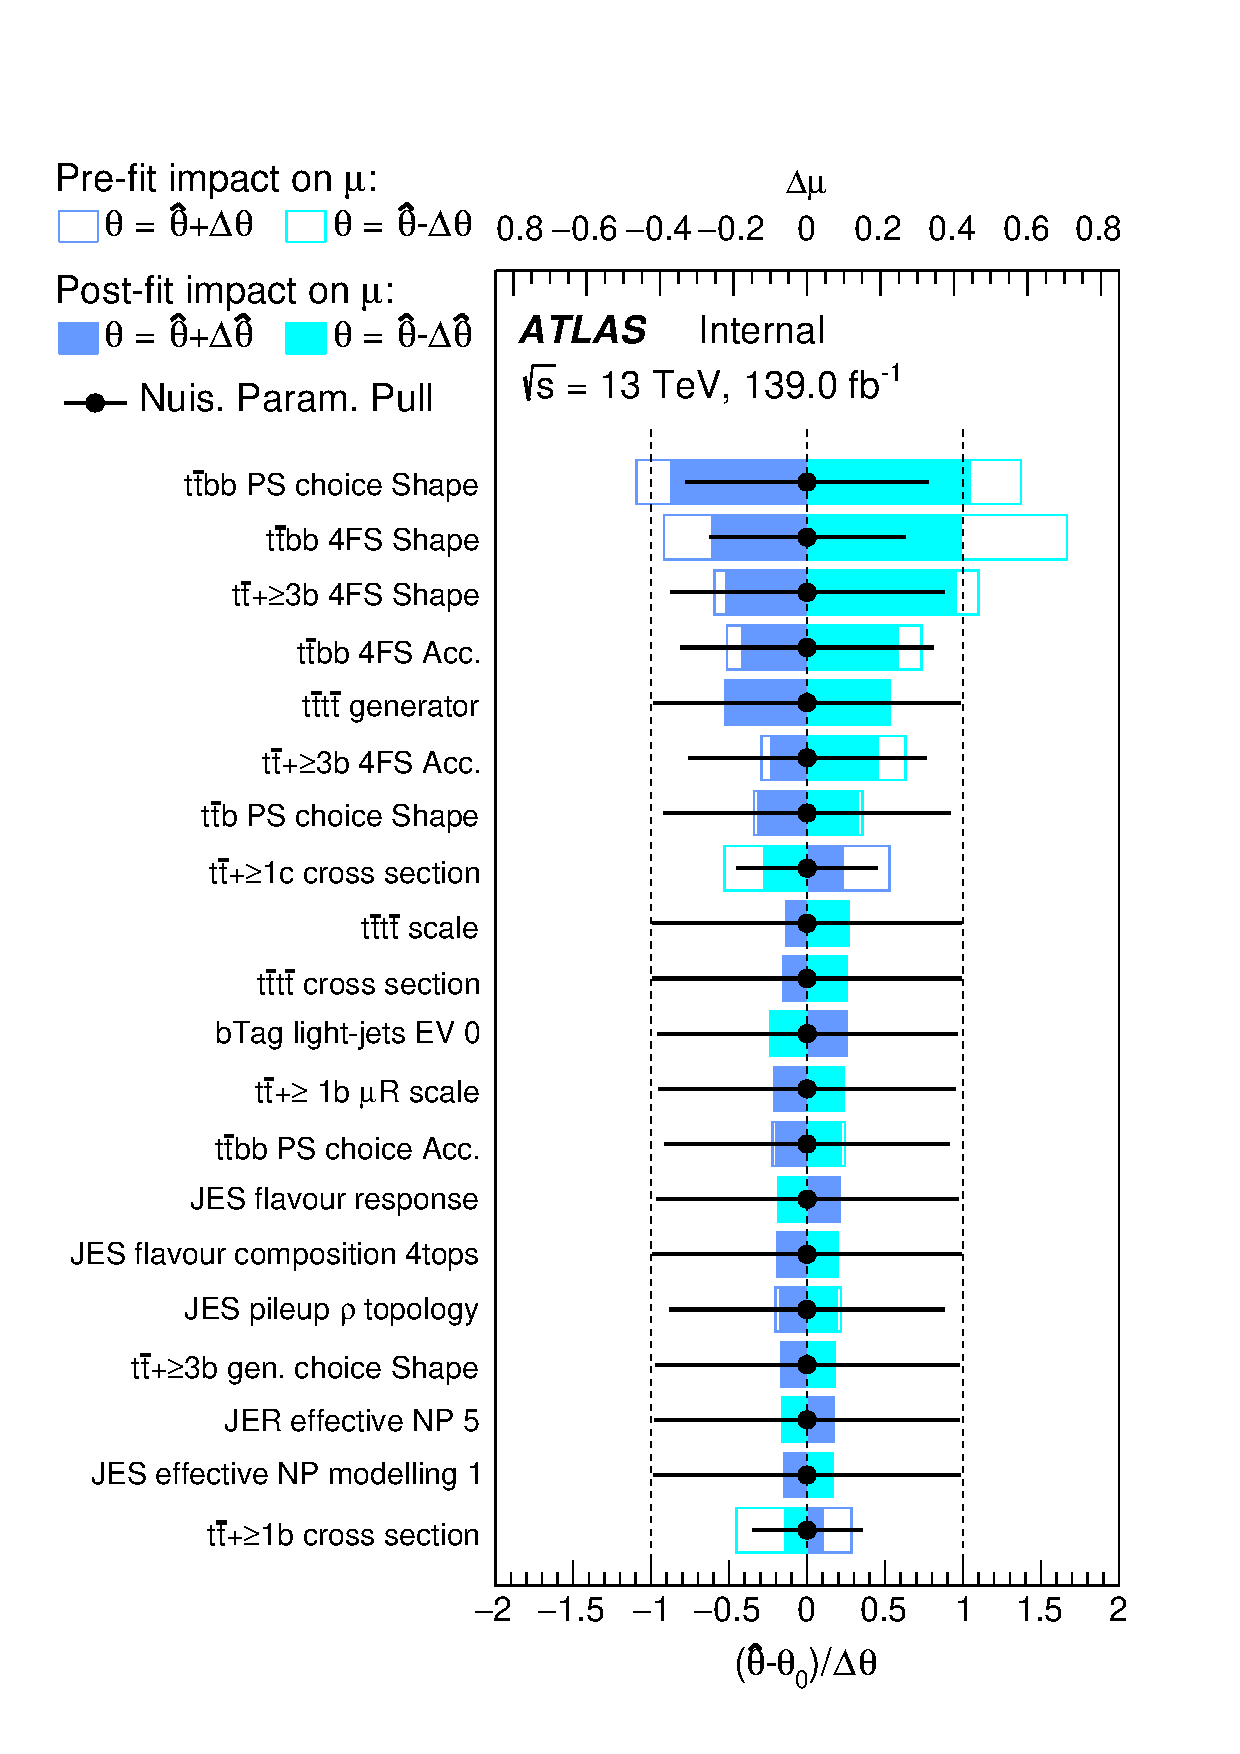
\includegraphics[width=\linewidth]{figures/fits/GNN/400/2L/asimov/Ranking_mu_tttt.pdf}
     \caption{\label{fig:Ranking_mH400_Asimov_2L}2L }
  \end{subfigure}
  \begin{subfigure}[t]{0.32\textwidth}
    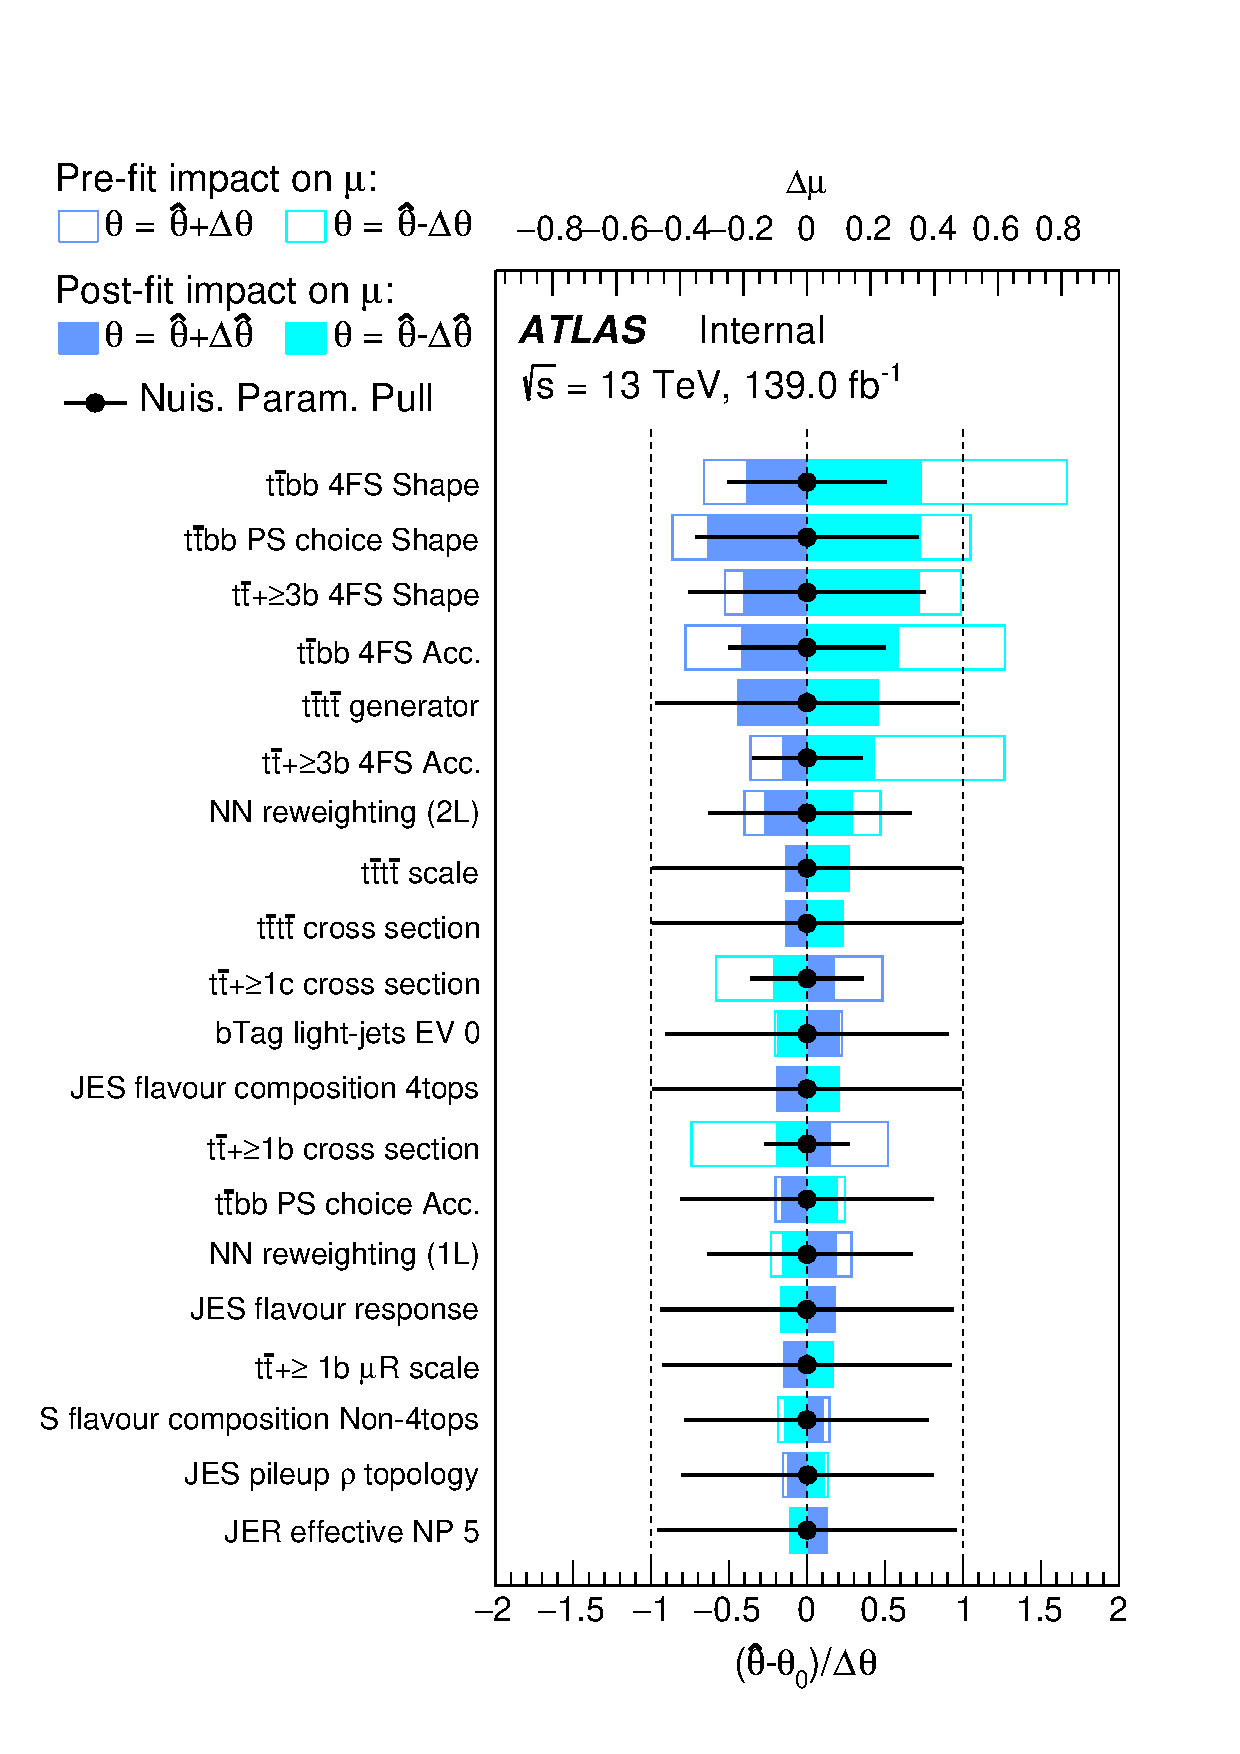
\includegraphics[width=\linewidth]{figures/fits/GNN/400/all/asimov/Ranking_mu_tttt.pdf}
     \caption{\label{fig:Ranking_mH400_Asimov_all}1L+2L }
  \end{subfigure}
  \caption{\label{fig:Ranking_mH400_Asimov}Fitted pulls and constraints for the nuisance parameters ranked by their impact for mH=400\gev for three types of Asimov fit: using only 1L regions, using only 2L regions and using all regions.}
\end{figure}


\begin{figure}[htbp!]
  \centering
  \begin{subfigure}[t]{0.32\textwidth}
    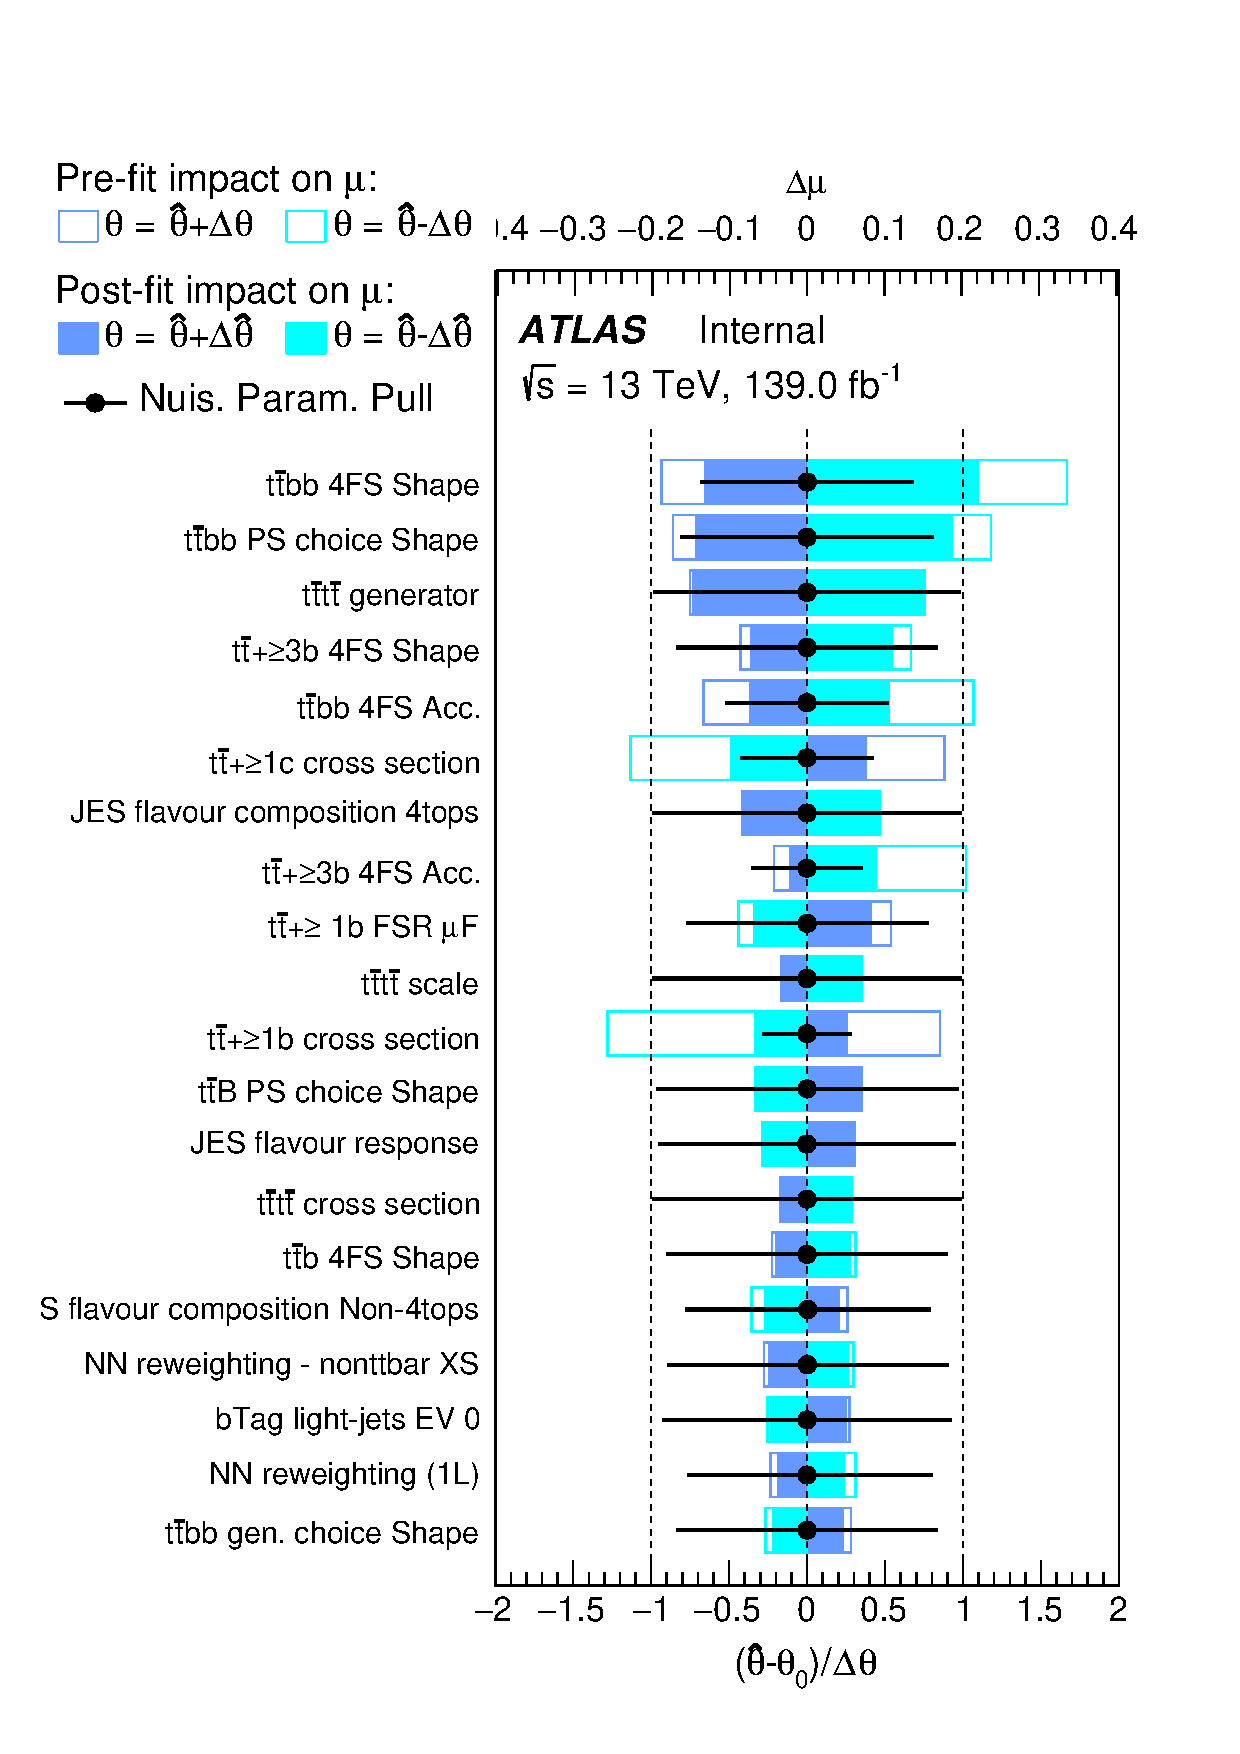
\includegraphics[width=\linewidth]{figures/fits/GNN/700/1L/asimov/Ranking_mu_tttt.pdf}
     \caption{\label{fig:Ranking_mH700_Asimov_1L}1L }
  \end{subfigure}
  \begin{subfigure}[t]{0.32\textwidth}
    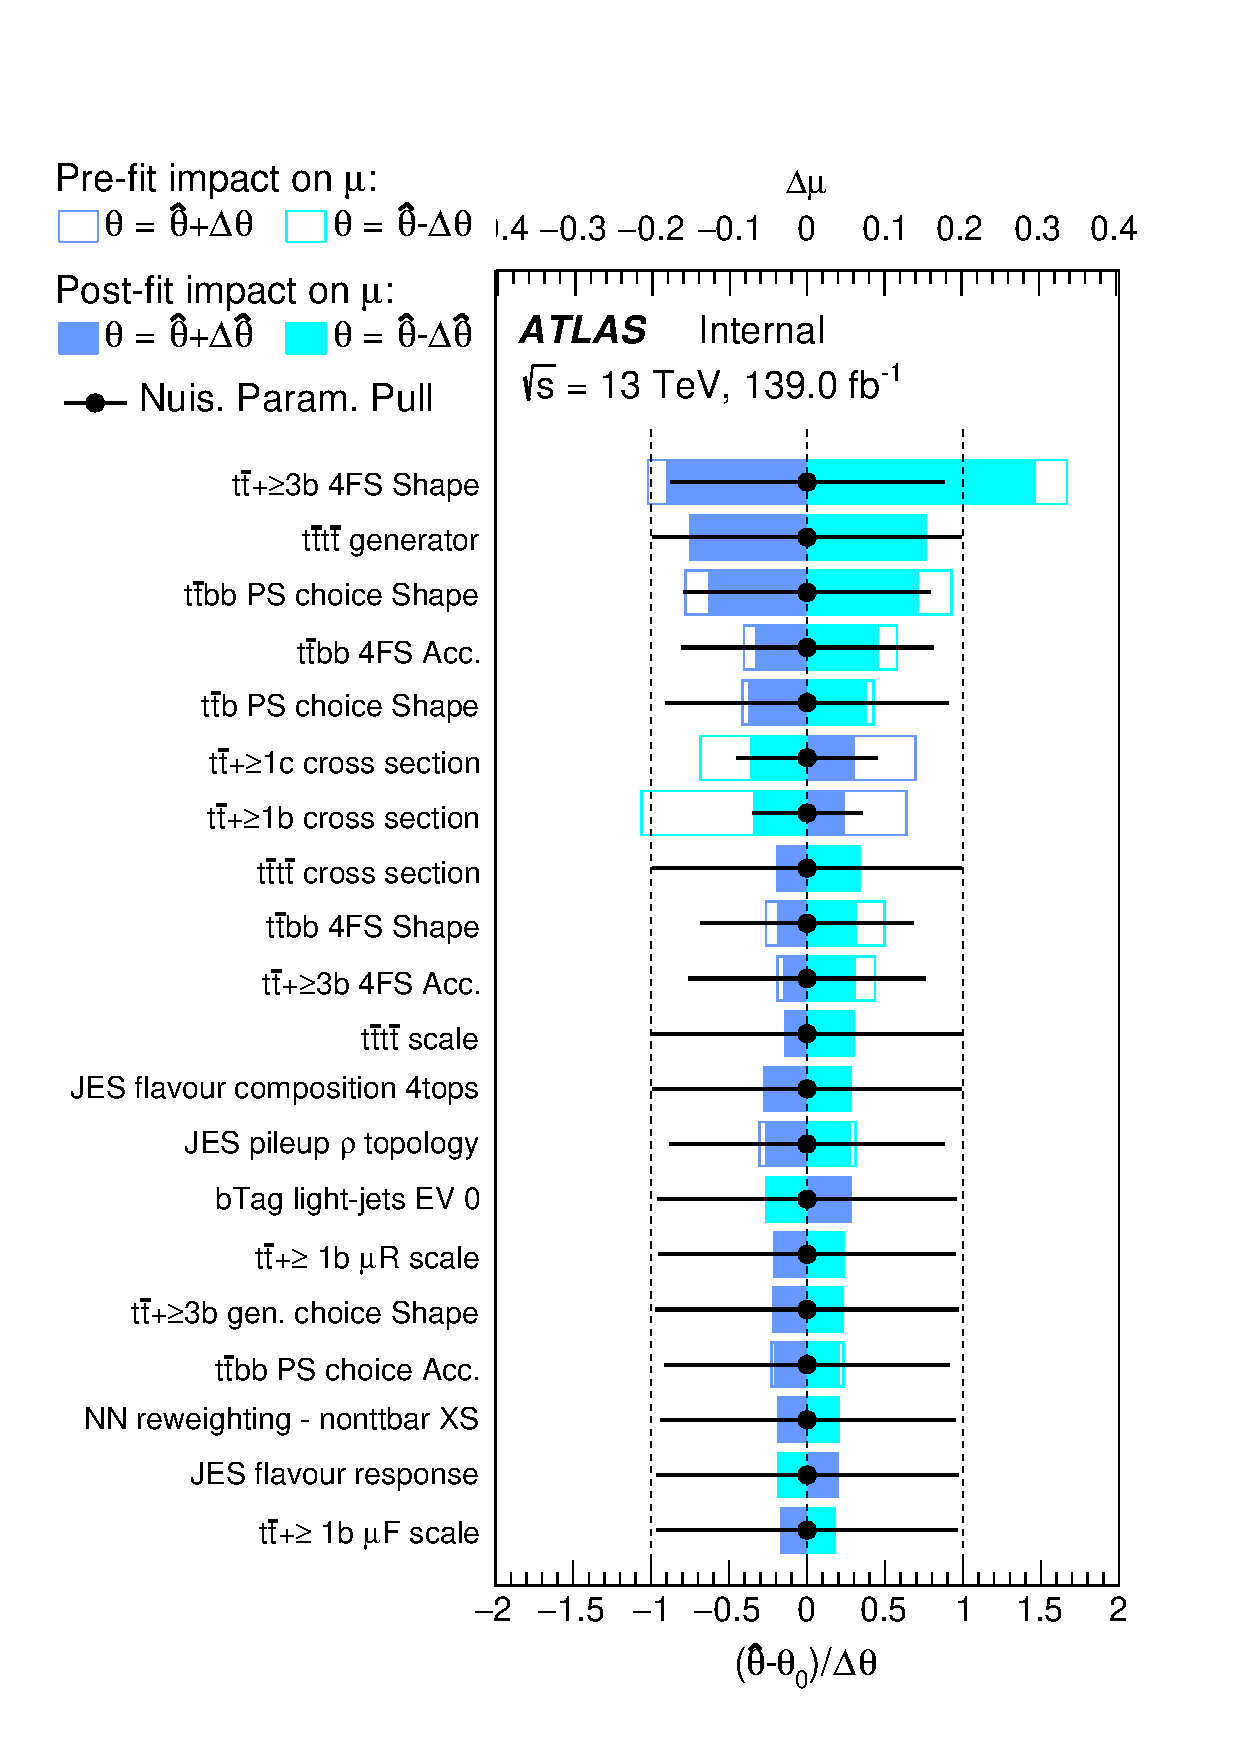
\includegraphics[width=\linewidth]{figures/fits/GNN/700/2L/asimov/Ranking_mu_tttt.pdf}
     \caption{\label{fig:Ranking_mH700_Asimov_2L}2L }
  \end{subfigure}
  \begin{subfigure}[t]{0.32\textwidth}
    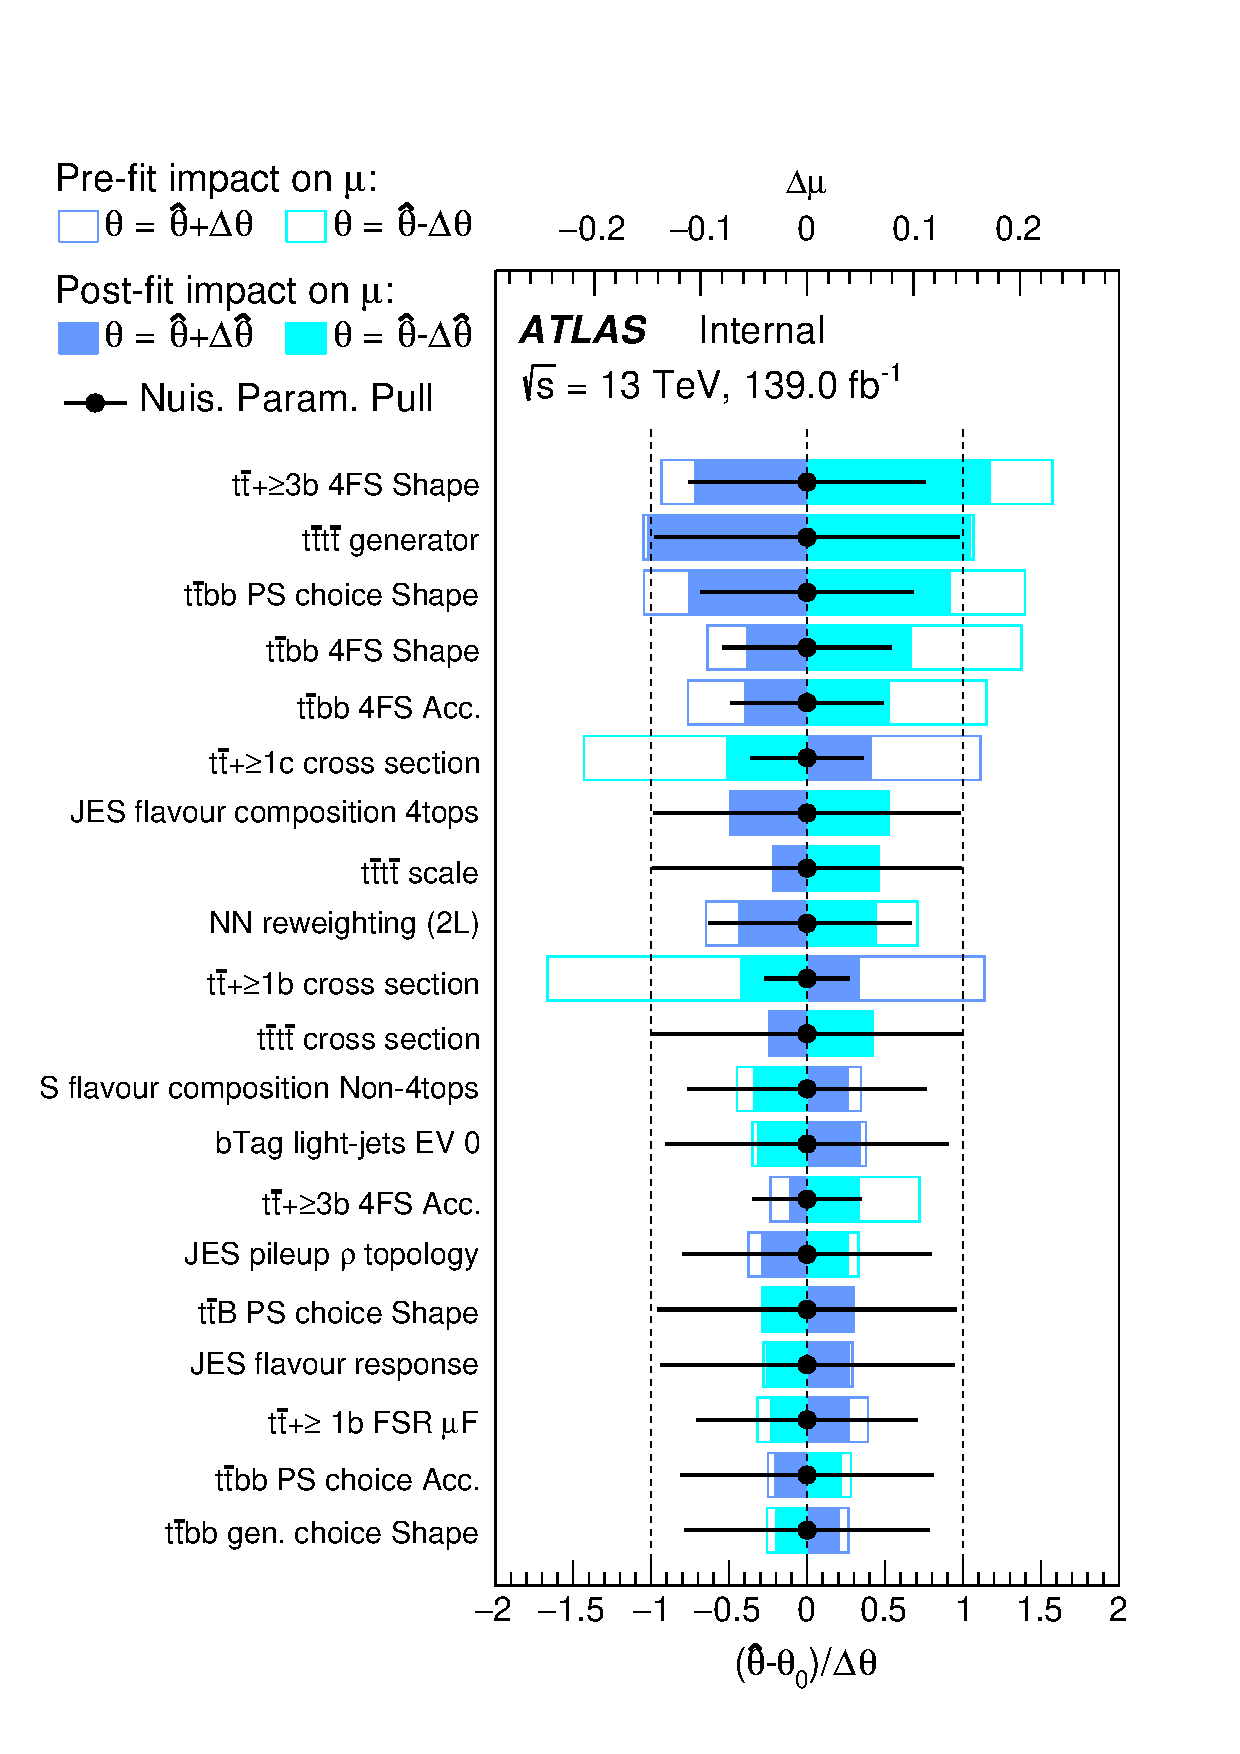
\includegraphics[width=\linewidth]{figures/fits/GNN/700/all/asimov/Ranking_mu_tttt.pdf}
     \caption{\label{fig:Ranking_mH700_Asimov_all}1L+2L }
  \end{subfigure}
  \caption{\label{fig:Ranking_mH700_Asimov}Fitted pulls and constraints for the nuisance parameters ranked by their impact for mH=700\gev for three types of Asimov fit: using only 1L regions, using only 2L regions and using all regions.}
\end{figure}

\begin{figure}[htbp!]
  \centering
  \begin{subfigure}[t]{0.32\textwidth}
    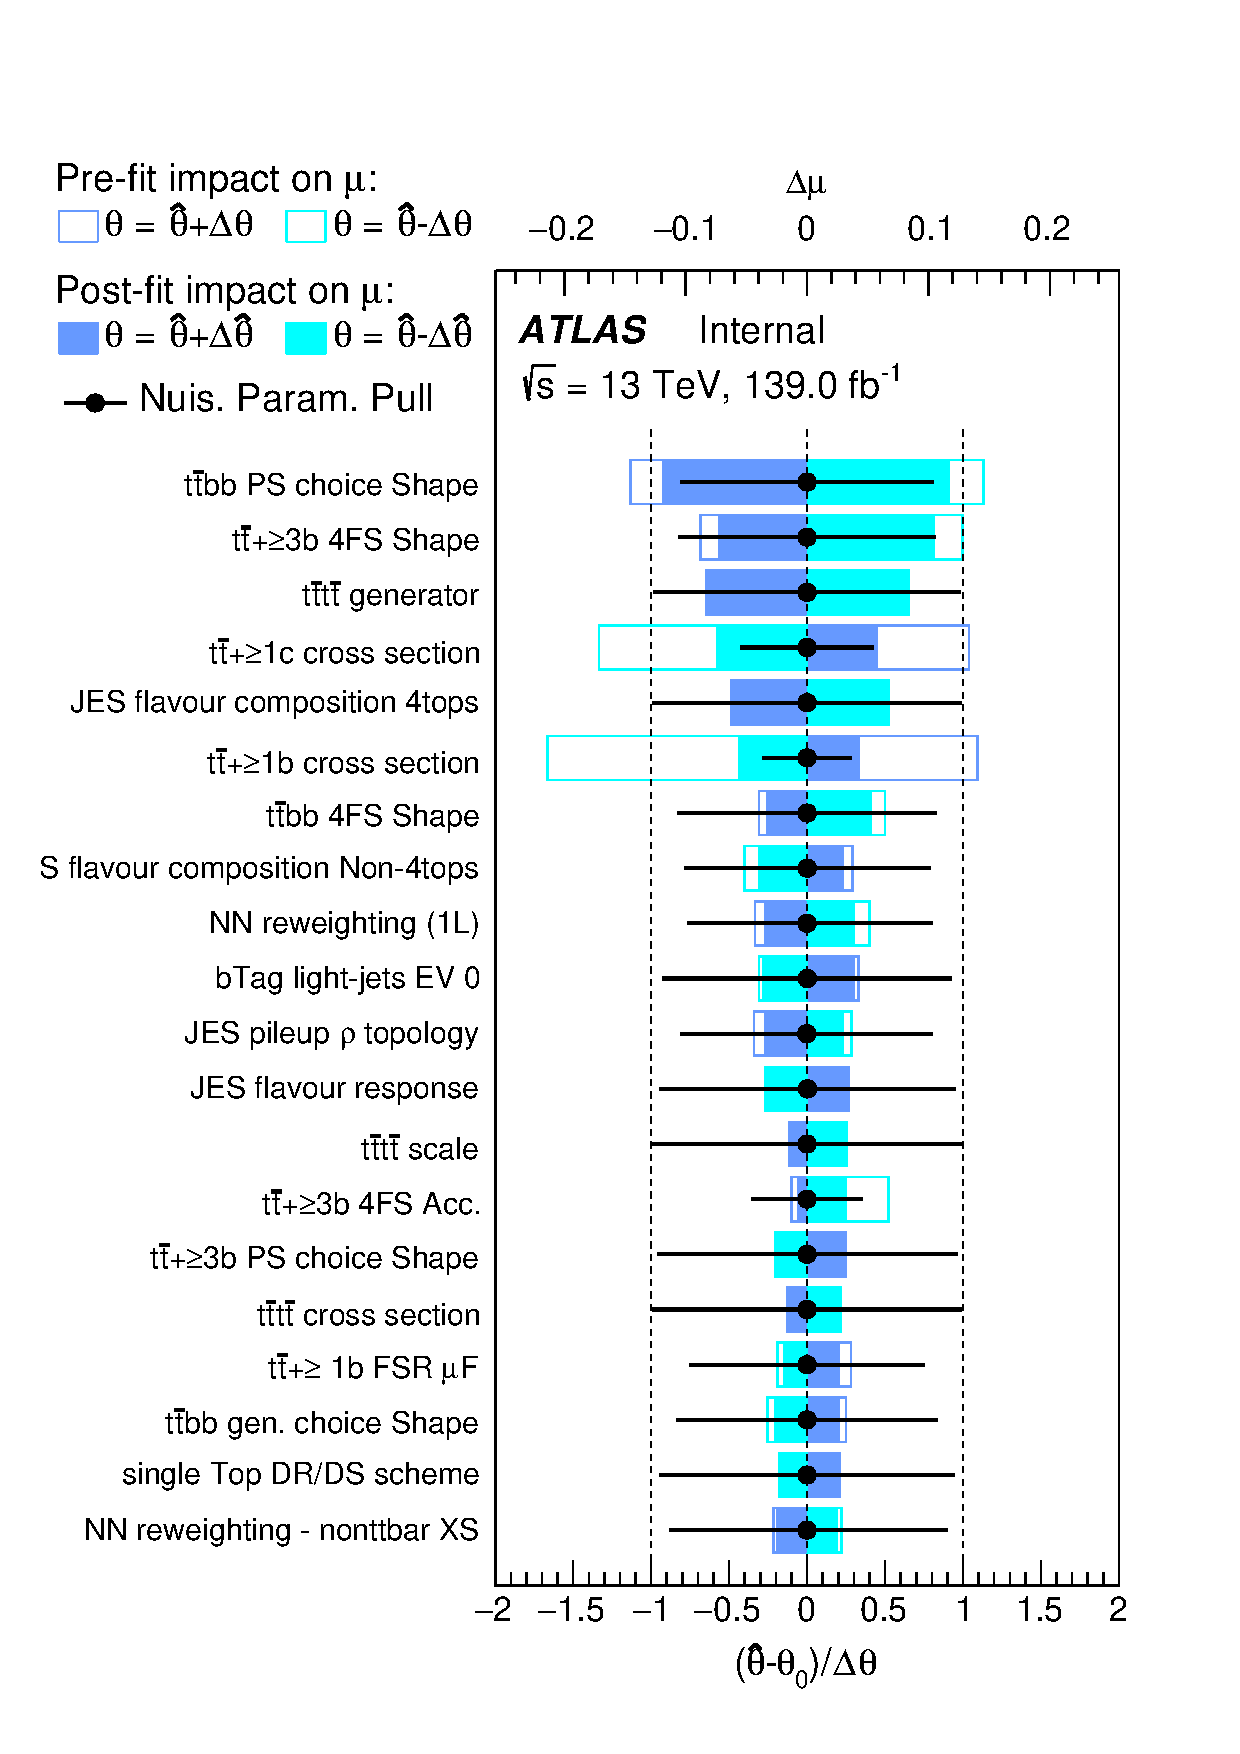
\includegraphics[width=\linewidth]{figures/fits/GNN/1000/1L/asimov/Ranking_mu_tttt.pdf}
     \caption{\label{fig:Ranking_mH1000_Asimov_1L}1L }
  \end{subfigure}
  \begin{subfigure}[t]{0.32\textwidth}
    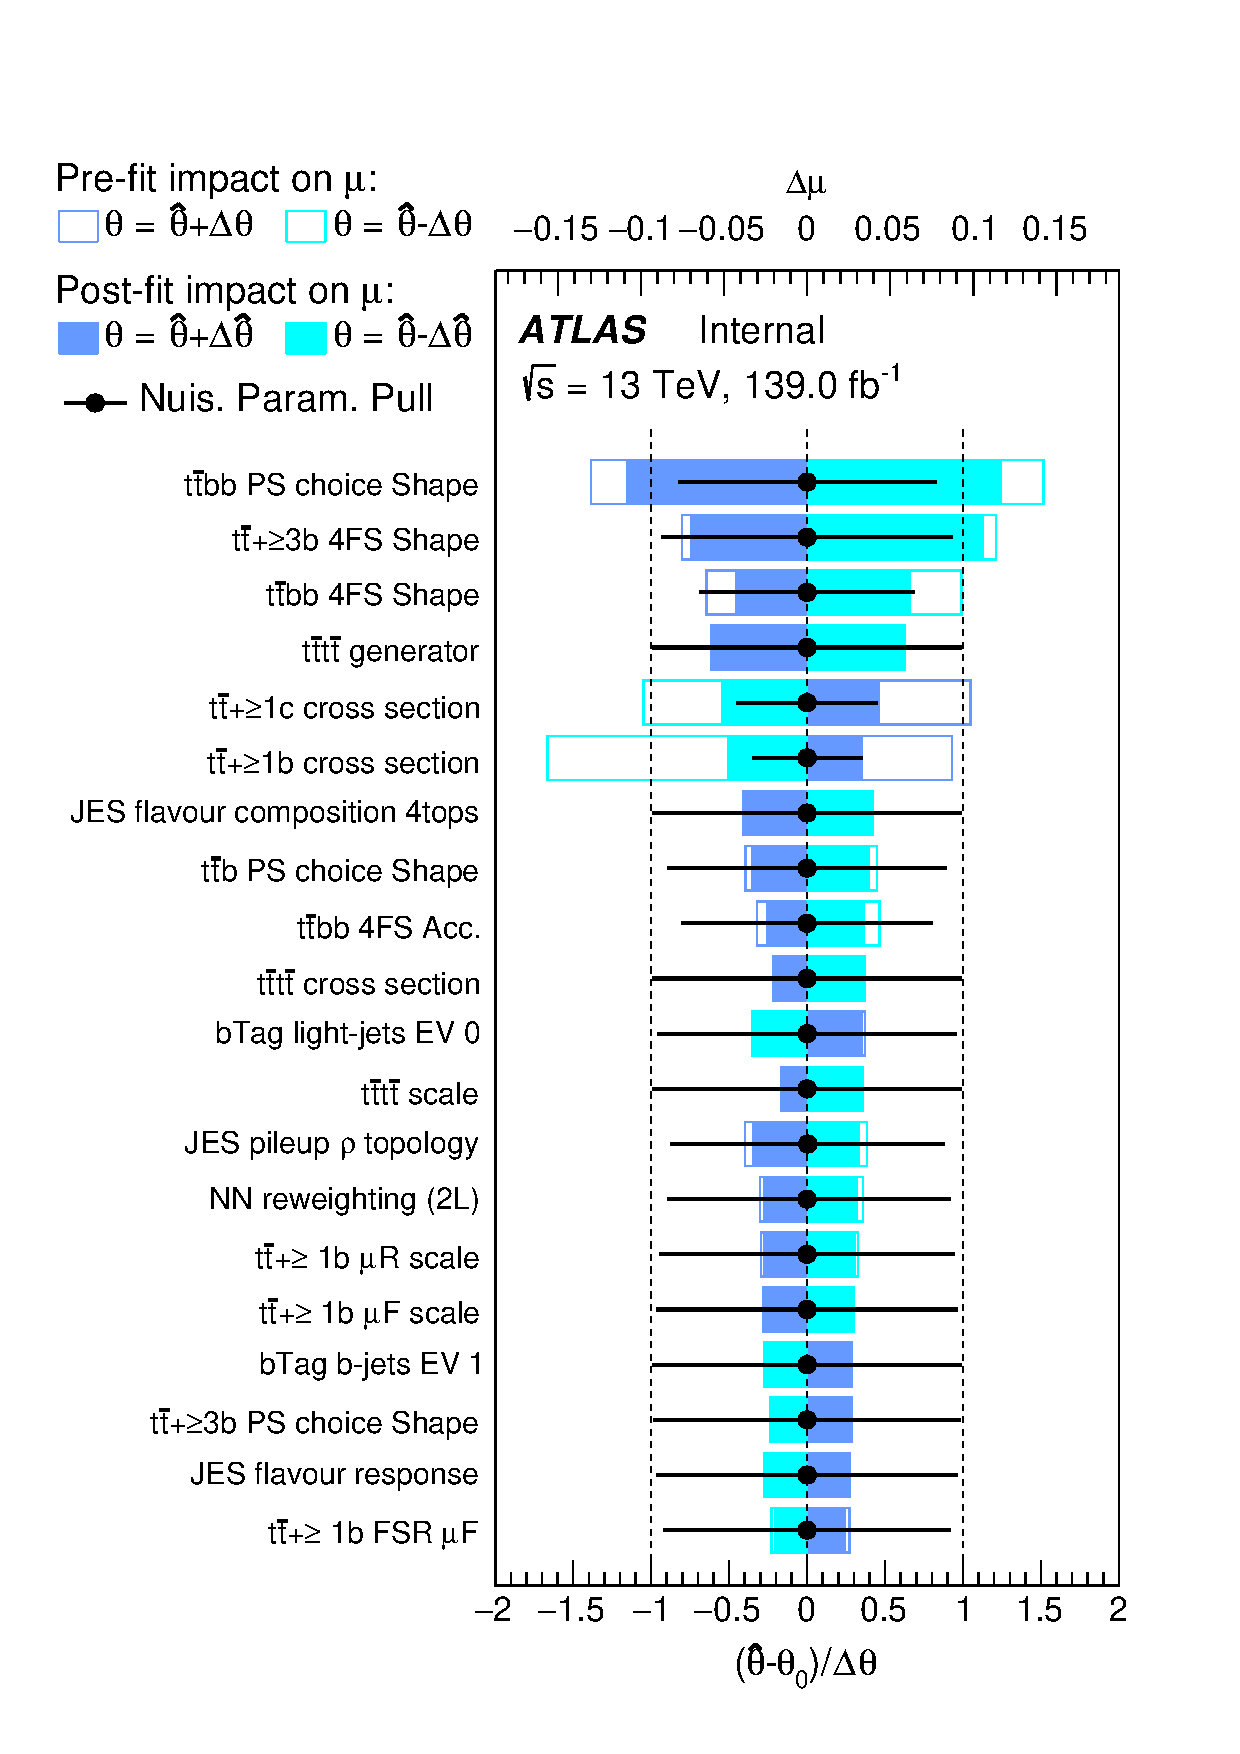
\includegraphics[width=\linewidth]{figures/fits/GNN/1000/2L/asimov/Ranking_mu_tttt.pdf}
     \caption{\label{fig:Ranking_mH1000_Asimov_2L}2L }
  \end{subfigure}
  \begin{subfigure}[t]{0.32\textwidth}
    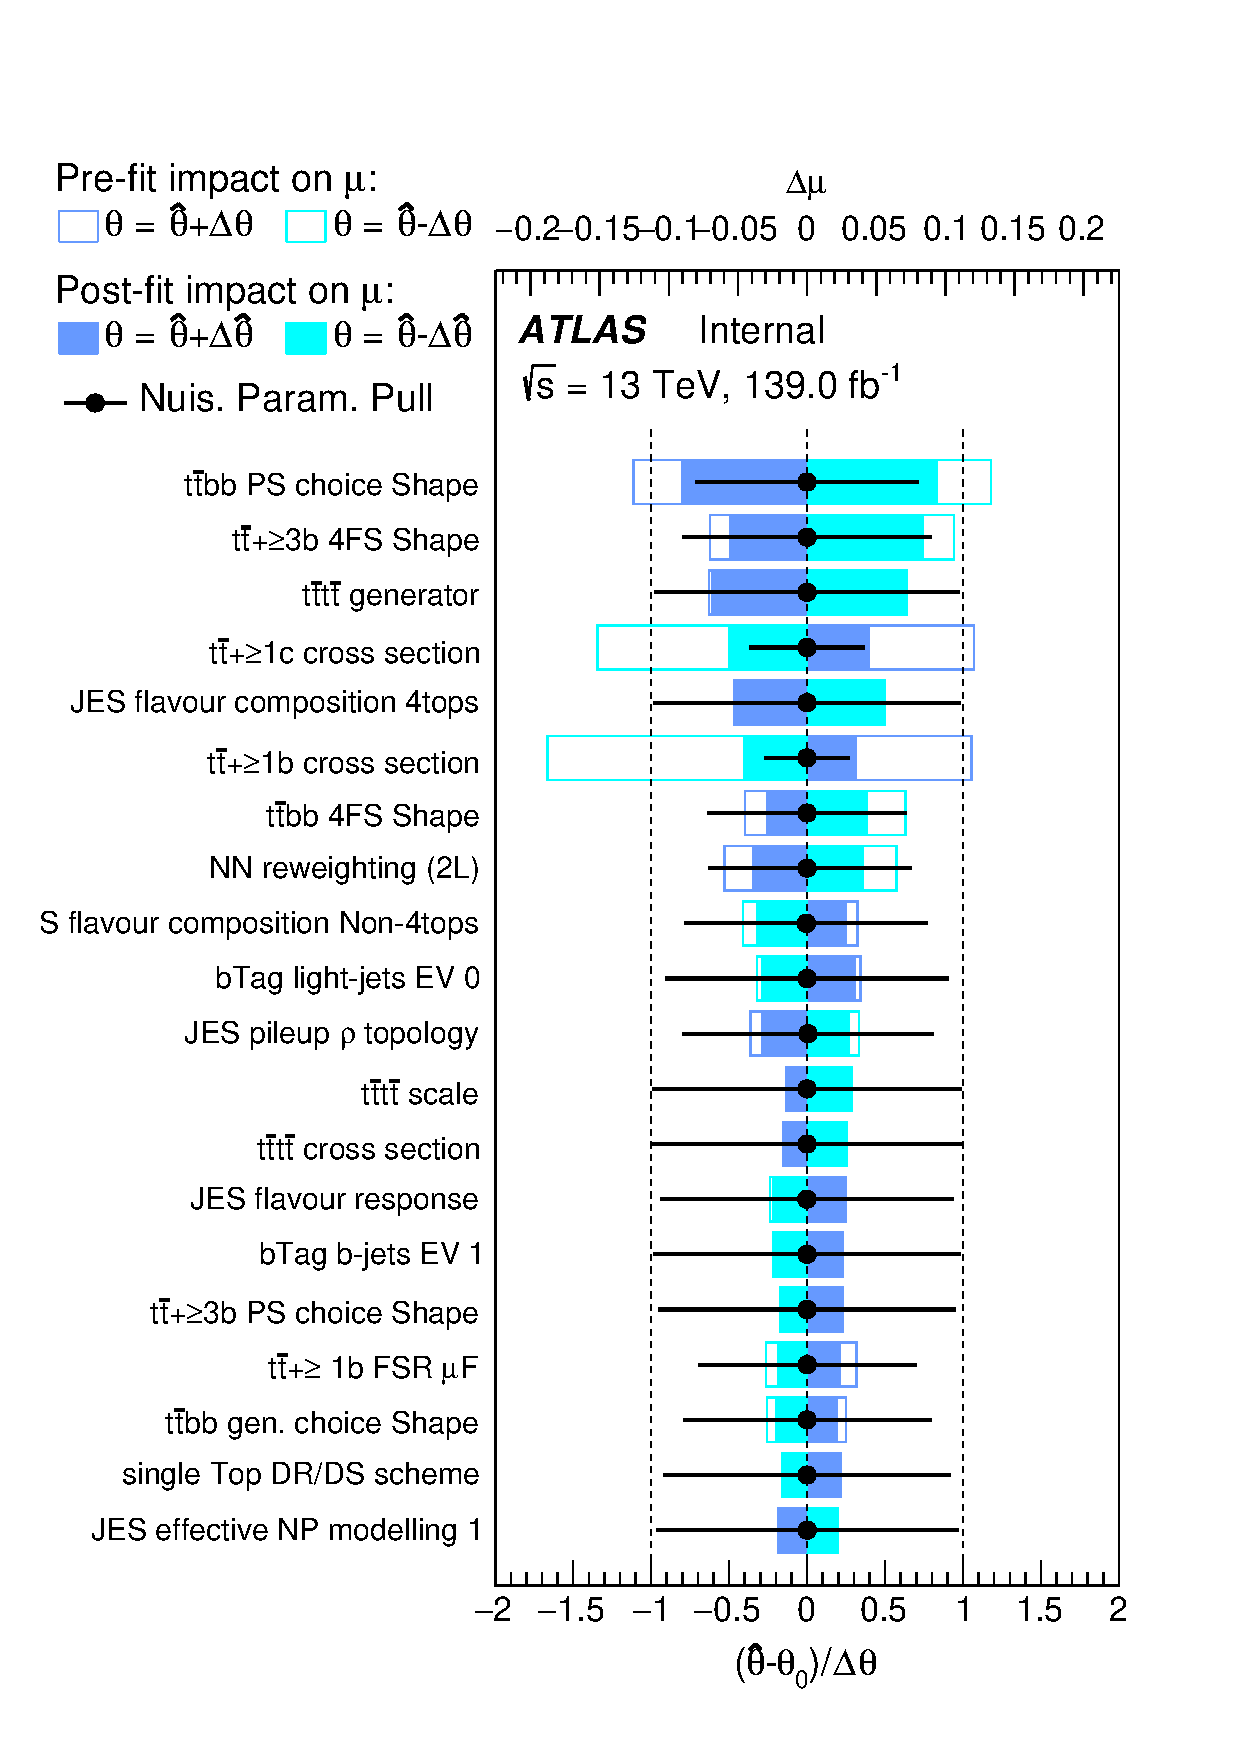
\includegraphics[width=\linewidth]{figures/fits/GNN/1000/all/asimov/Ranking_mu_tttt.pdf}
     \caption{\label{fig:Ranking_mH1000_Asimov_all}1L+2L }
  \end{subfigure}
  \caption{\label{fig:Ranking_mH1000_Asimov}Fitted pulls and constraints for the nuisance parameters ranked by their impact for mH=1000\gev for three types of Asimov fit: using only 1L regions, using only 2L regions and using all regions.}
\end{figure}


%\begin{figure}[htbp!]
%  \centering
%  \begin{subfigure}[t]{0.32\textwidth}
%    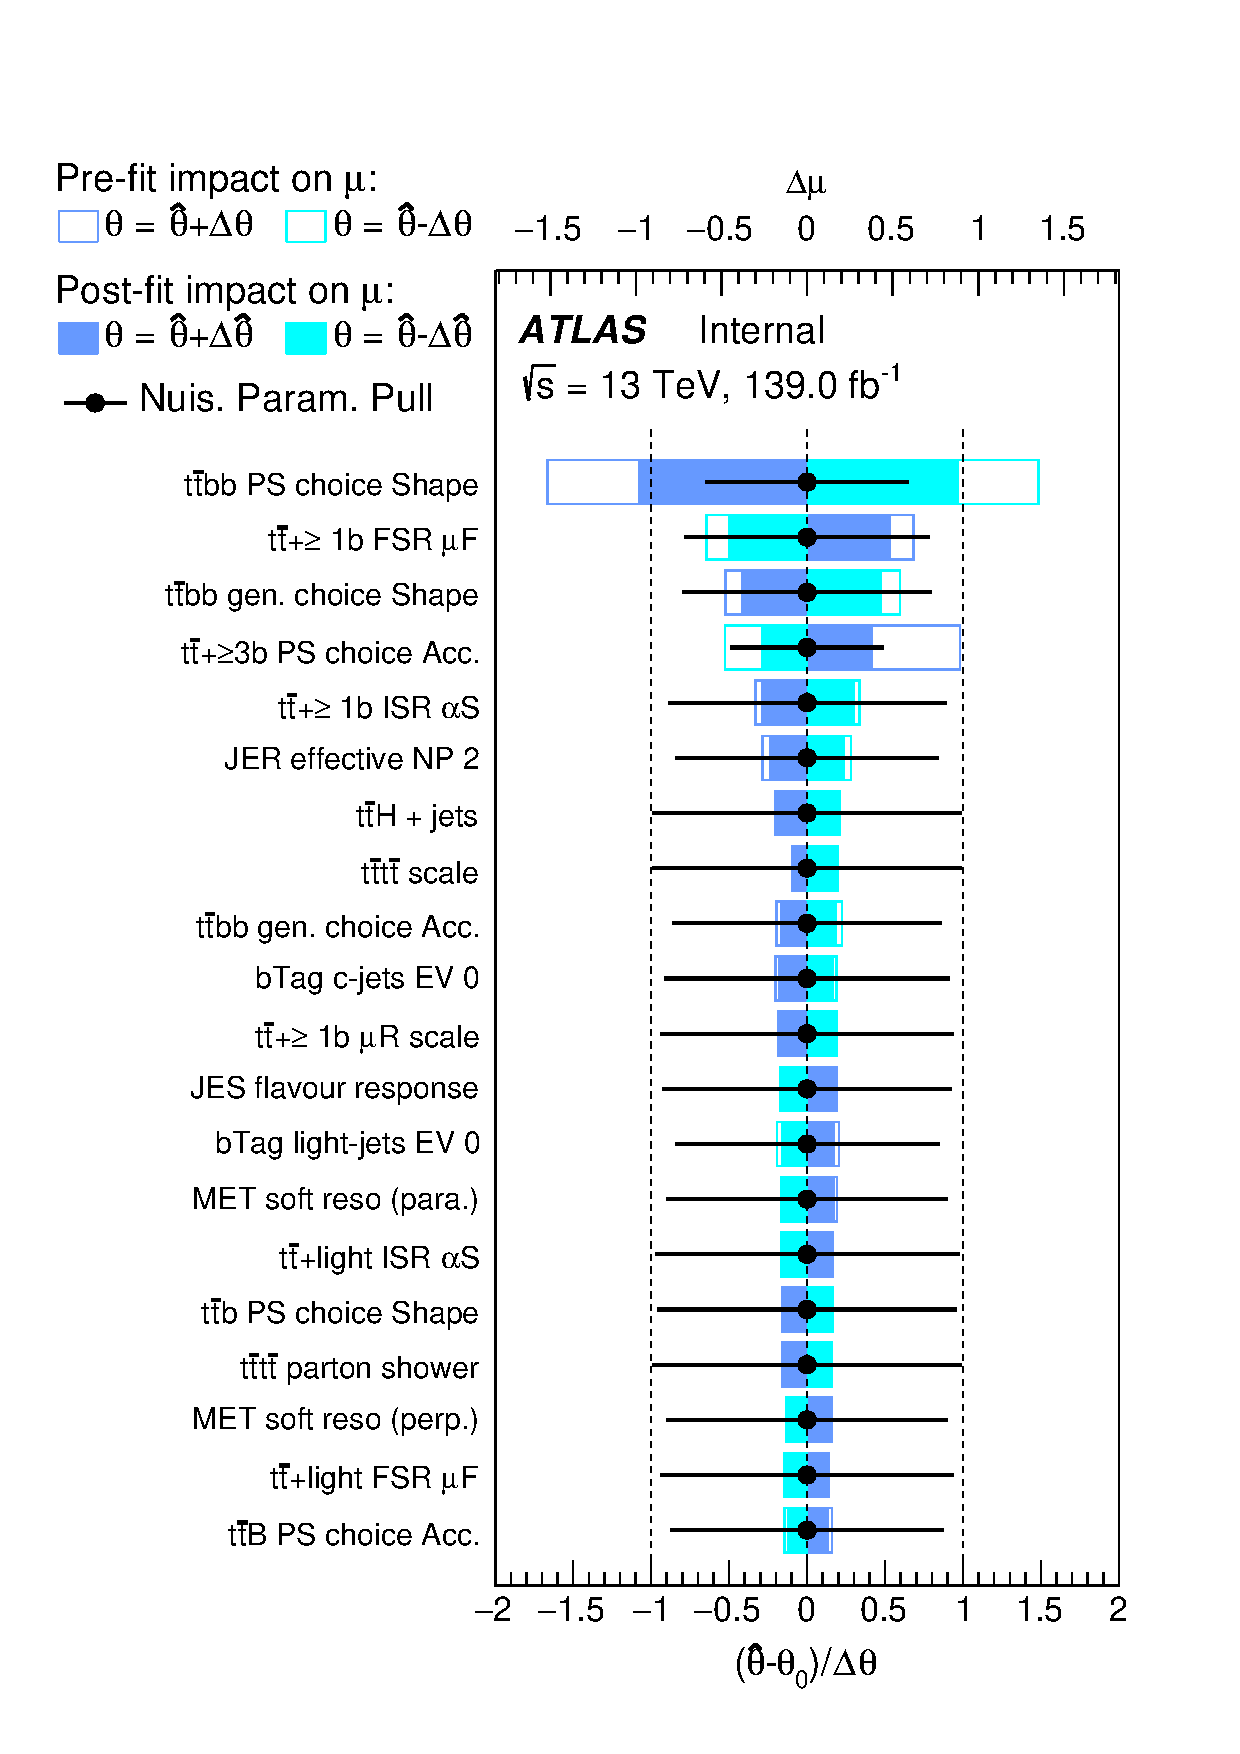
\includegraphics[width=\linewidth]{figures/fits/BDT/400/1L/asimov/Ranking_mu_tttt.pdf}
%     \caption{\label{fig:Ranking_mH400_Asimov_1L}1L }
%  \end{subfigure}
%  \begin{subfigure}[t]{0.32\textwidth}
%    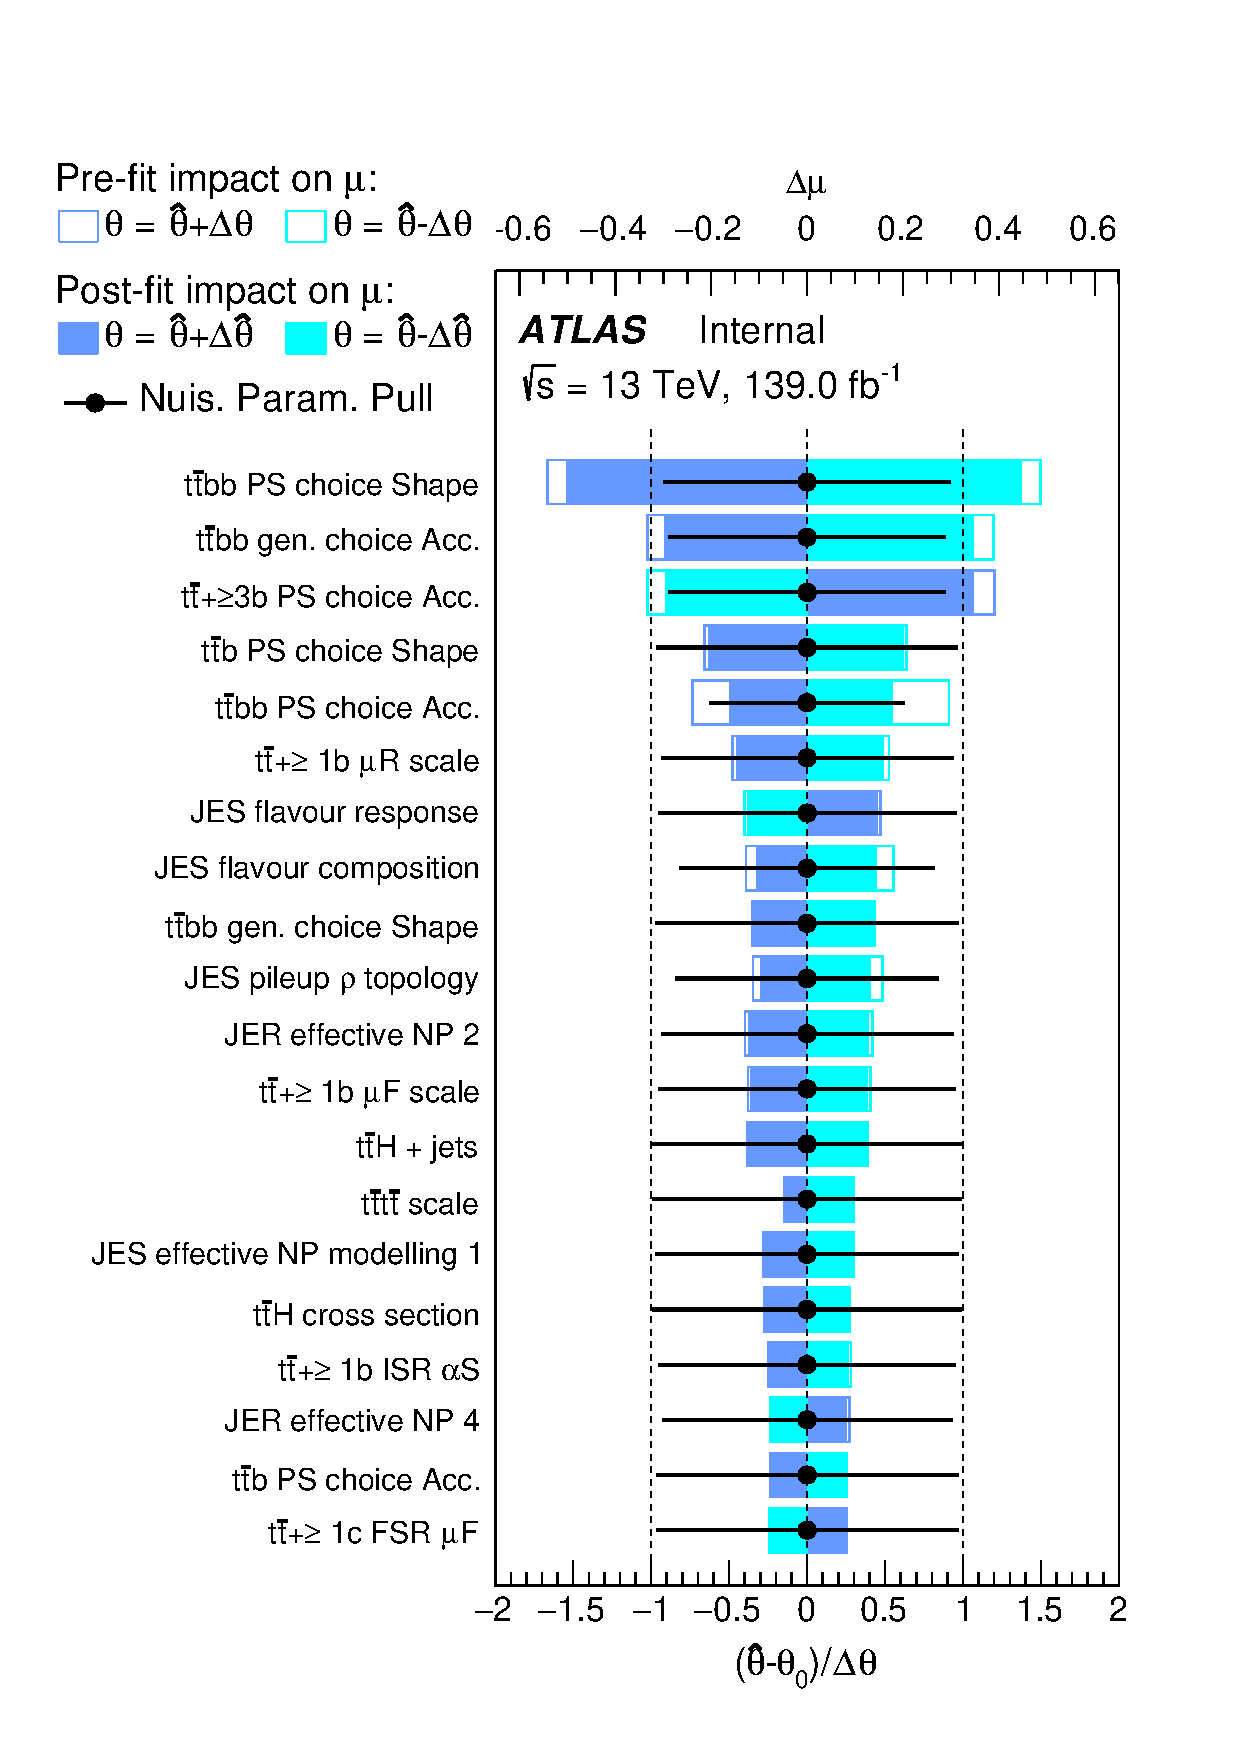
\includegraphics[width=\linewidth]{figures/fits/BDT/400/2L/asimov/Ranking_mu_tttt.pdf}
%     \caption{\label{fig:Ranking_mH400_Asimov_2L}2L }
%  \end{subfigure}
%  \begin{subfigure}[t]{0.32\textwidth}
%    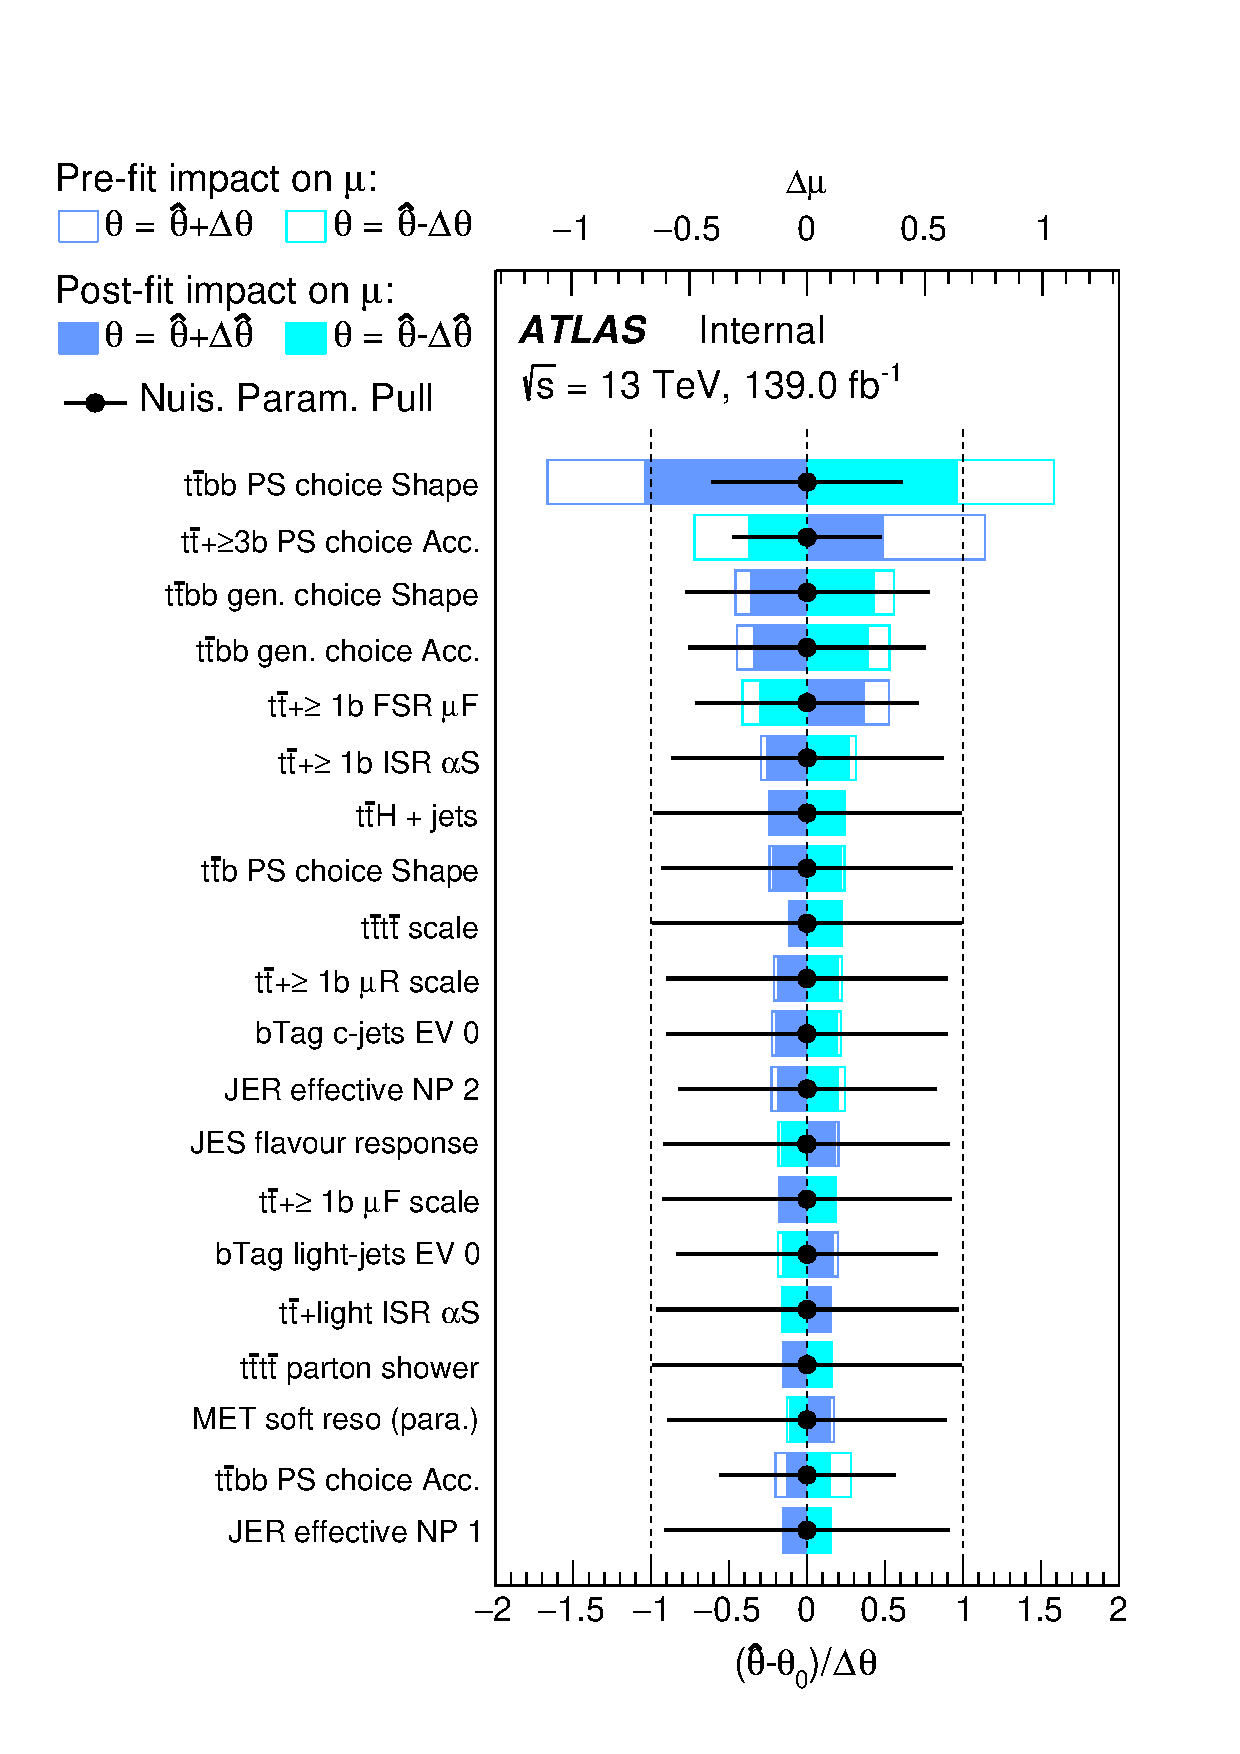
\includegraphics[width=\linewidth]{figures/fits/BDT/400/all/asimov/Ranking_mu_tttt.pdf}
%     \caption{\label{fig:Ranking_mH400_Asimov_all}1L+2L }
%  \end{subfigure}
%  \caption{\label{fig:Ranking_mH400_Asimov_BDT}Fitted pulls and constraints for the nuisance parameters ranked by their impact for mH=400\gev for three types of Asimov fit: using only 1L regions, using only 2L regions and using all regions. These fits use the BDT output distribution for the signal regions as opposed to the above fits which use GNN.}
%\end{figure}




\begin{figure}[htbp!]
        \centering
        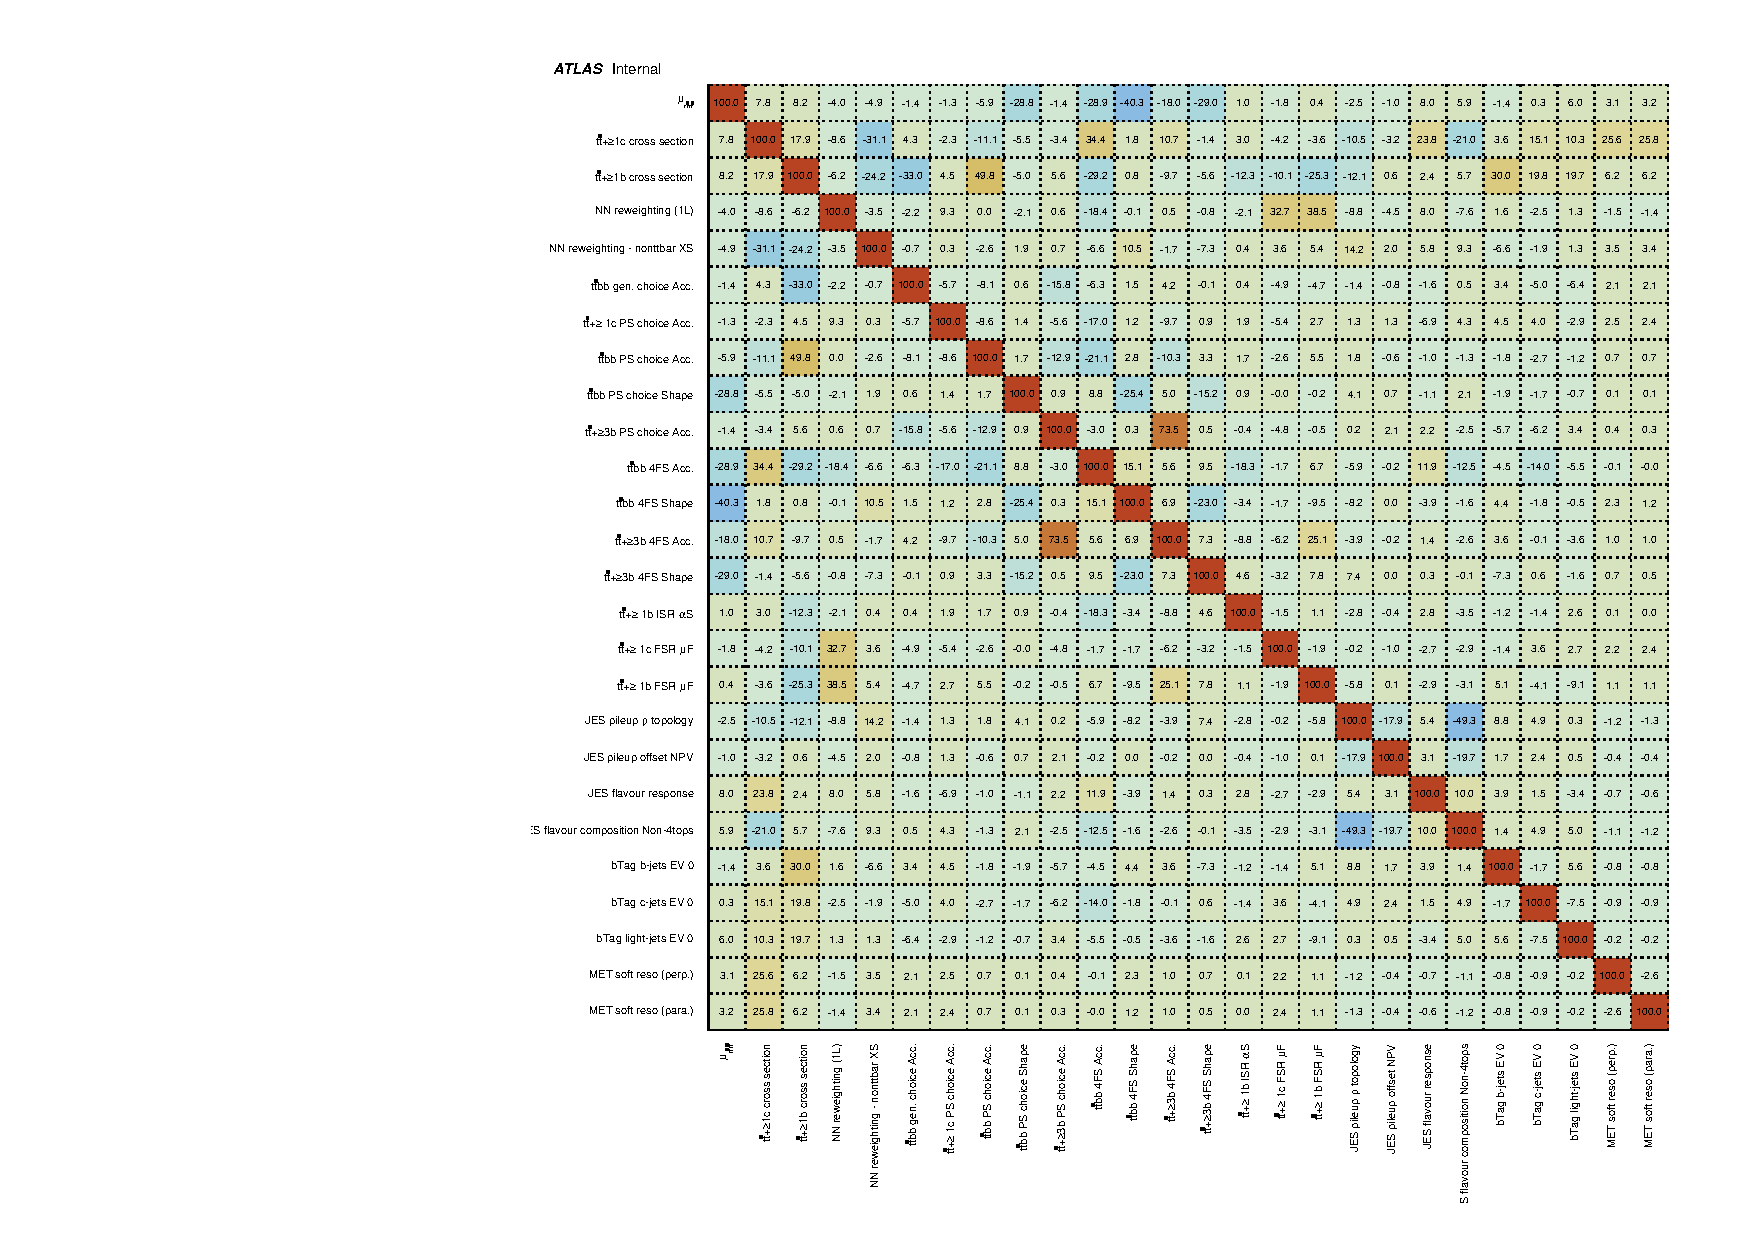
\includegraphics[width=\linewidth]{figures/fits/GNN/400/1L/asimov/CorrMatrix.pdf}
        \caption{\label{fig:Corr_mH400_Asimov_1L}Correlation matrix for the 1L Asimov fit for mH = 400 GeV}
\end{figure}

\begin{figure}[htbp!]
        \centering
        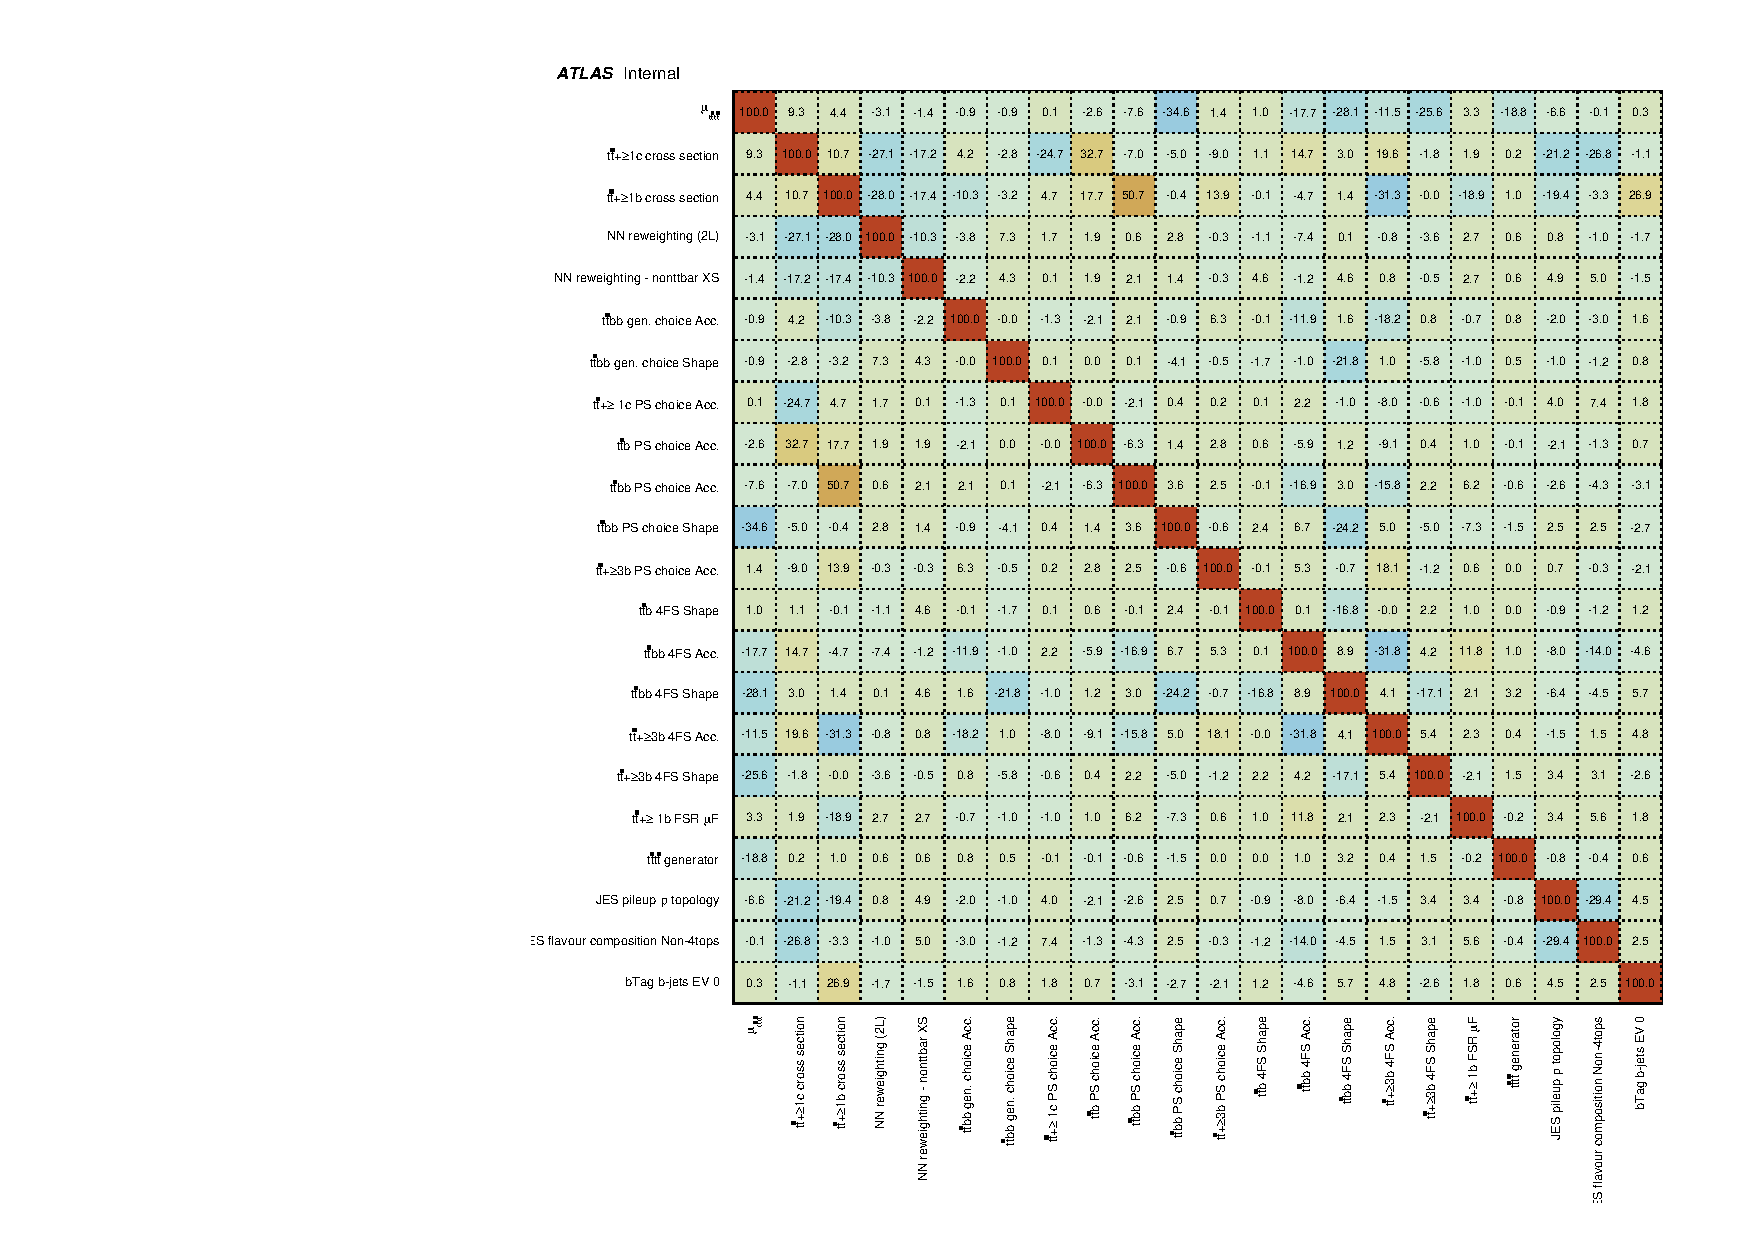
\includegraphics[width=\linewidth]{figures/fits/GNN/400/2L/asimov/CorrMatrix.pdf}
        \caption{\label{fig:Corr_mH400_Asimov_2L}Correlation matrix for the 2LOS Asimov fit for mH = 400 GeV}
\end{figure}

\begin{figure}[htbp!]
        \centering
        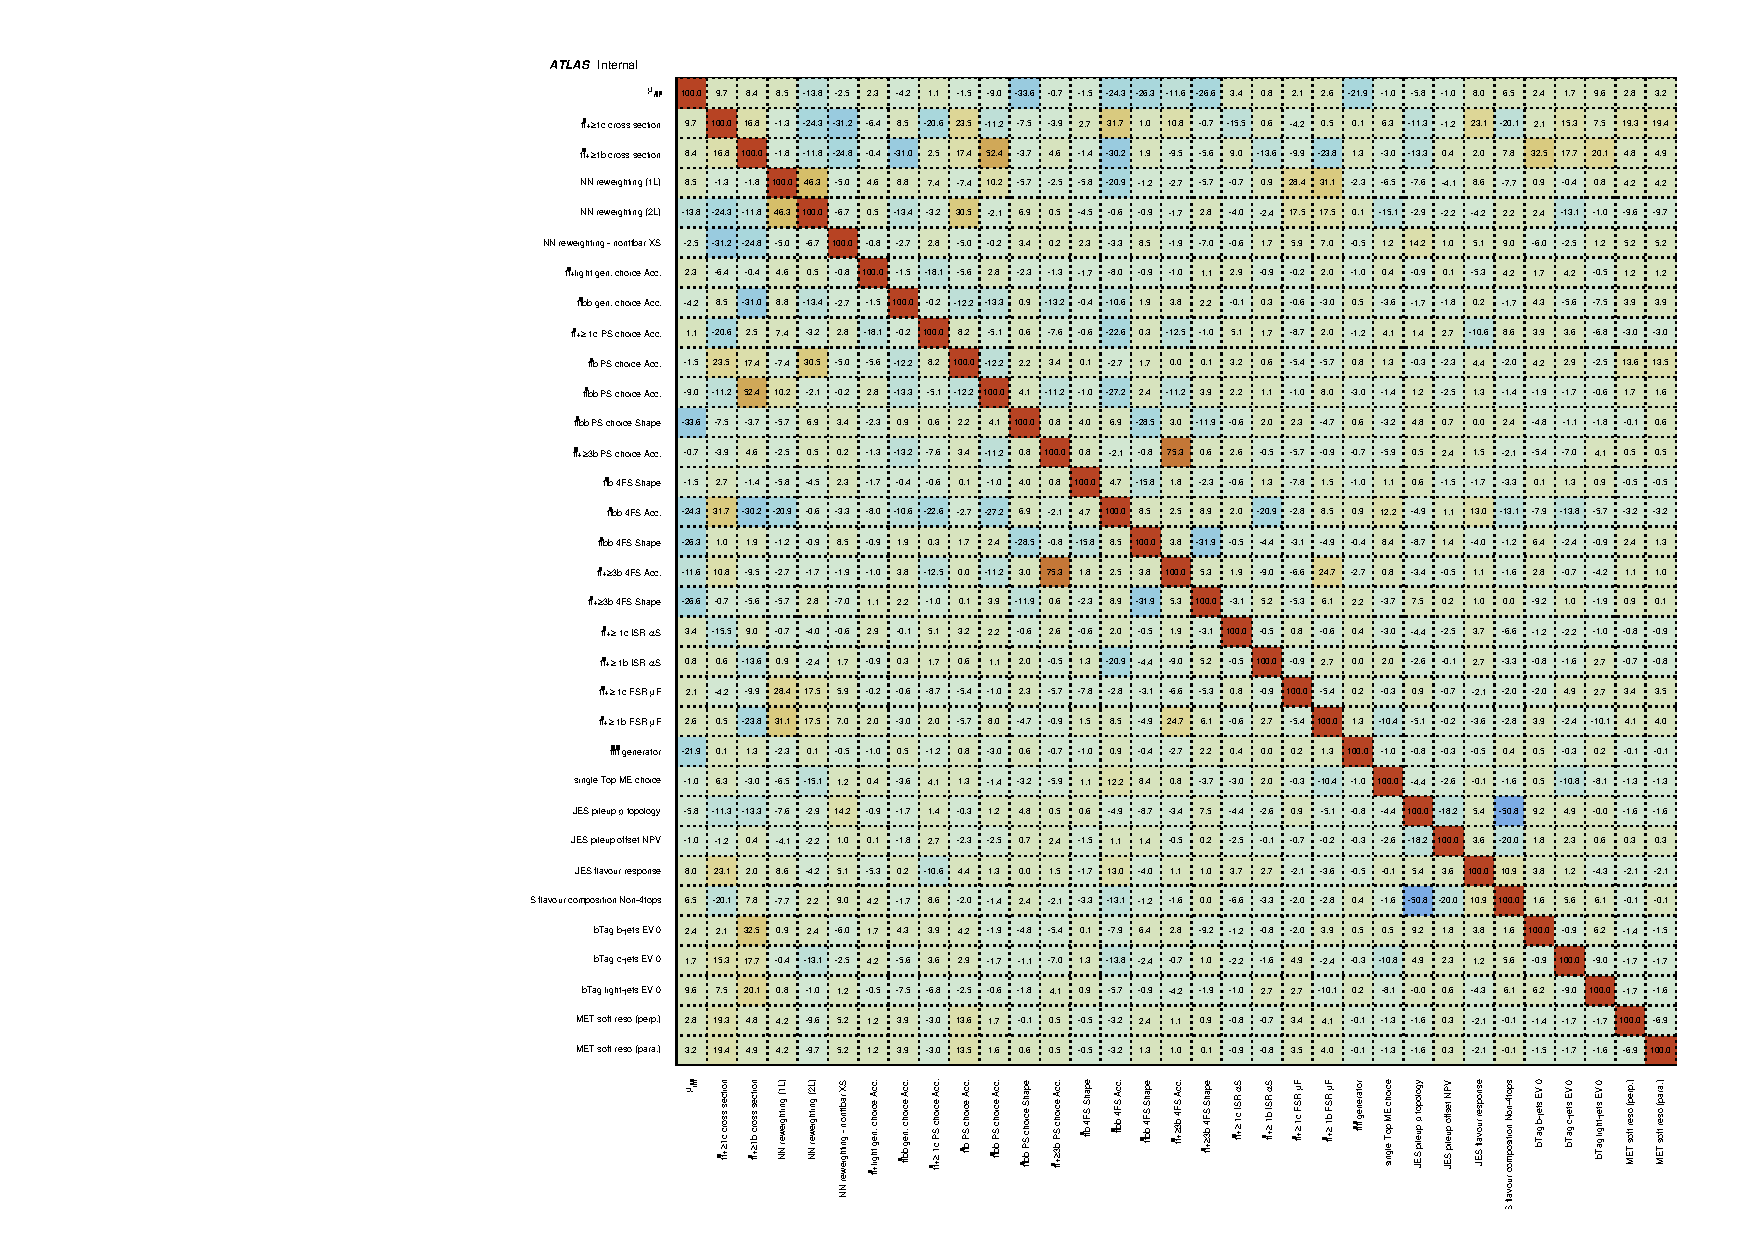
\includegraphics[width=\linewidth]{figures/fits/GNN/400/all/asimov/CorrMatrix.pdf}
        \caption{\label{fig:Corr_mH400_Asimov_all}Correlation matrix for the 1L/2LOS combined Asimov fit for mH = 400 GeV}
\end{figure}


%-------------------------------------------------------------------------------

%-------------------------------------------------------------------------------
\FloatBarrier
\section{Fits to blinded data}% Peter
\label{sec:blinded}
%
A fit using data is performed on using bins which are not blinded. The bins with S/B ratio of greater than 5\% are blinded in both pre-fit and post-fit yield plots. The signal sample is not included in the fit (it is a background-only fit). The blinded fit provides information on the modeling agreement in background-dominated regions of phase space, and systematics can be pulled from their initial value as well as constrained.

The blinded data fit is performed over all control and signal regions, and with all available samples and systematics. The dominant ttbar background is reweighted using the NN method.

The post-fit distributions associated with each background and signal region are shown in Figure \ref{fig:Postfit_Yields_1L} for 1L regions and Figure \ref{fig:Postfit_Yields_2L} for 2LOS regions from the combined fit using mass point $m_H=400$ GeV. The nuisance parameter pulls and constraints are compared between 1L, 2LOS, and the combined fit in Figures \ref{fig:data_NP_instrumental}, \ref{fig:data_NP_ttbar}, and \ref{fig:data_NP_other}. Comparison for the fits using GNN outputs trained on various mass points are shown in Figures \ref{fig:data_NP_mass_instrumental}, \ref{fig:data_NP_mass_ttbar}, and \ref{fig:data_NP_mass_other}.

Correlation matrices for systematics for 1L, 2LOS, and the combined fit are shown in Figure \ref{fig:Corr_mH400_Data_1L}, Figure \ref{fig:Corr_mH400_Data_2L}, and Figure \ref{fig:Corr_mH400_Data_all} respectively.

\begin{figure}[htbp!]
        \begin{center} \setlength{\tabcolsep}{2.5pt}\footnotesize
        \begin{tabular}{cccc}
        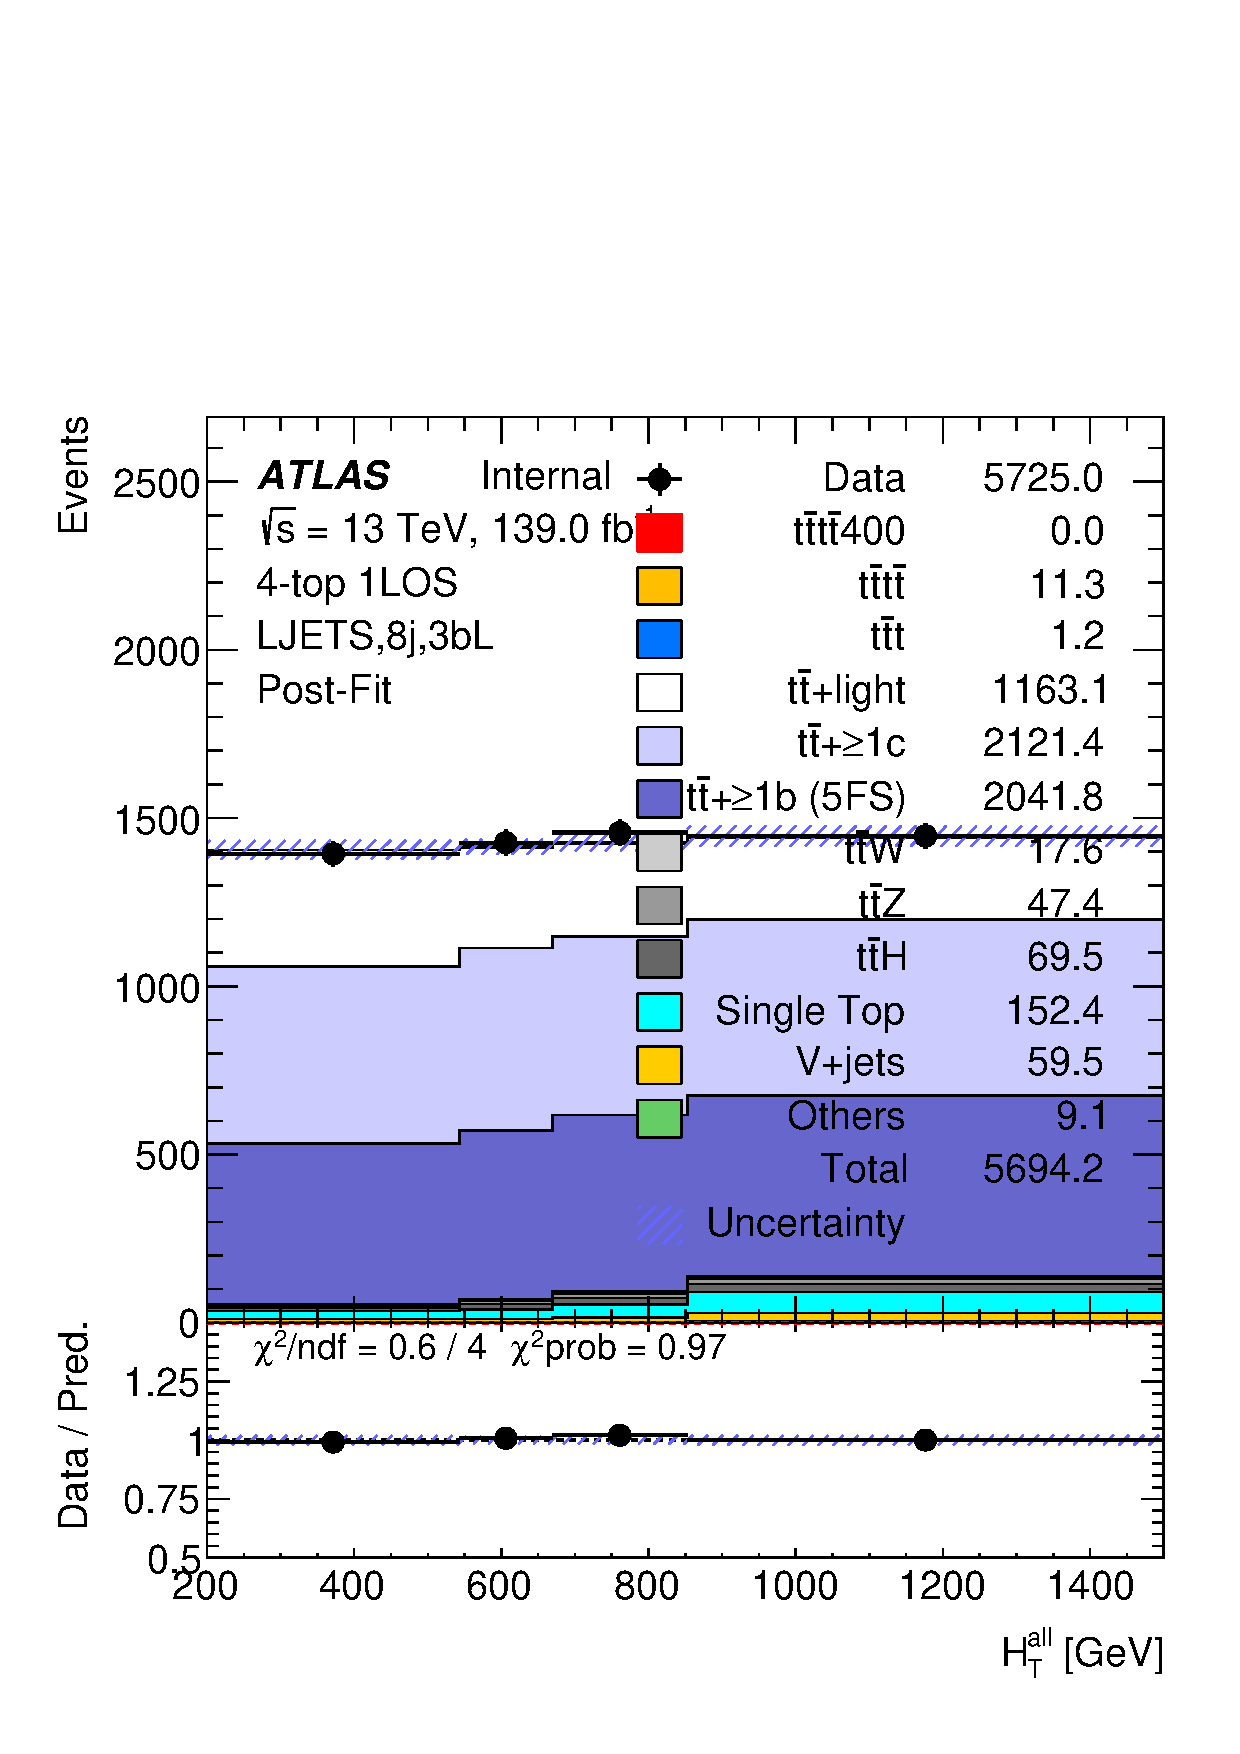
\includegraphics[width=0.23 \textwidth]{figures/fits/GNN/400/all/data/Plots/ljets_8j3bL_postFit.pdf} &
        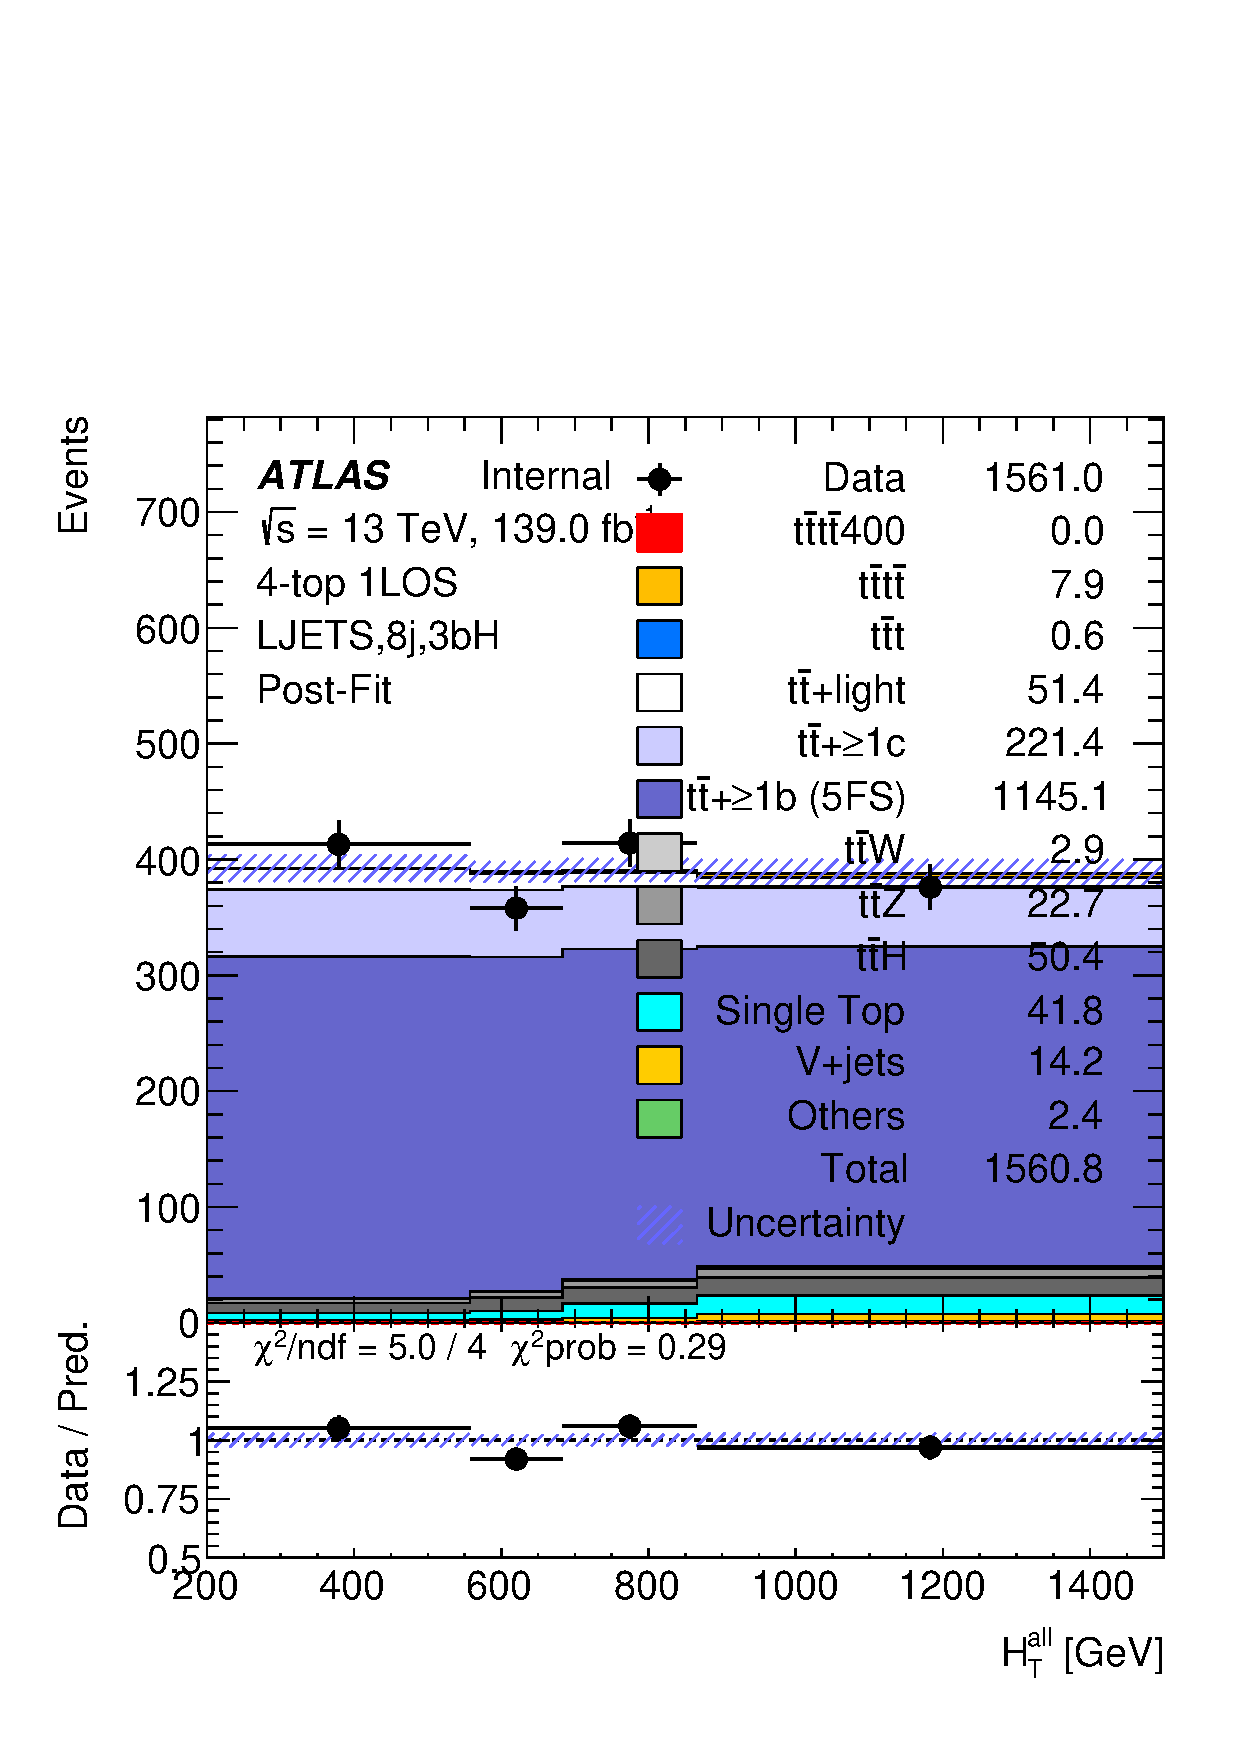
\includegraphics[width=0.23 \textwidth]{figures/fits/GNN/400/all/data/Plots/ljets_8j3bH_postFit.pdf} &
        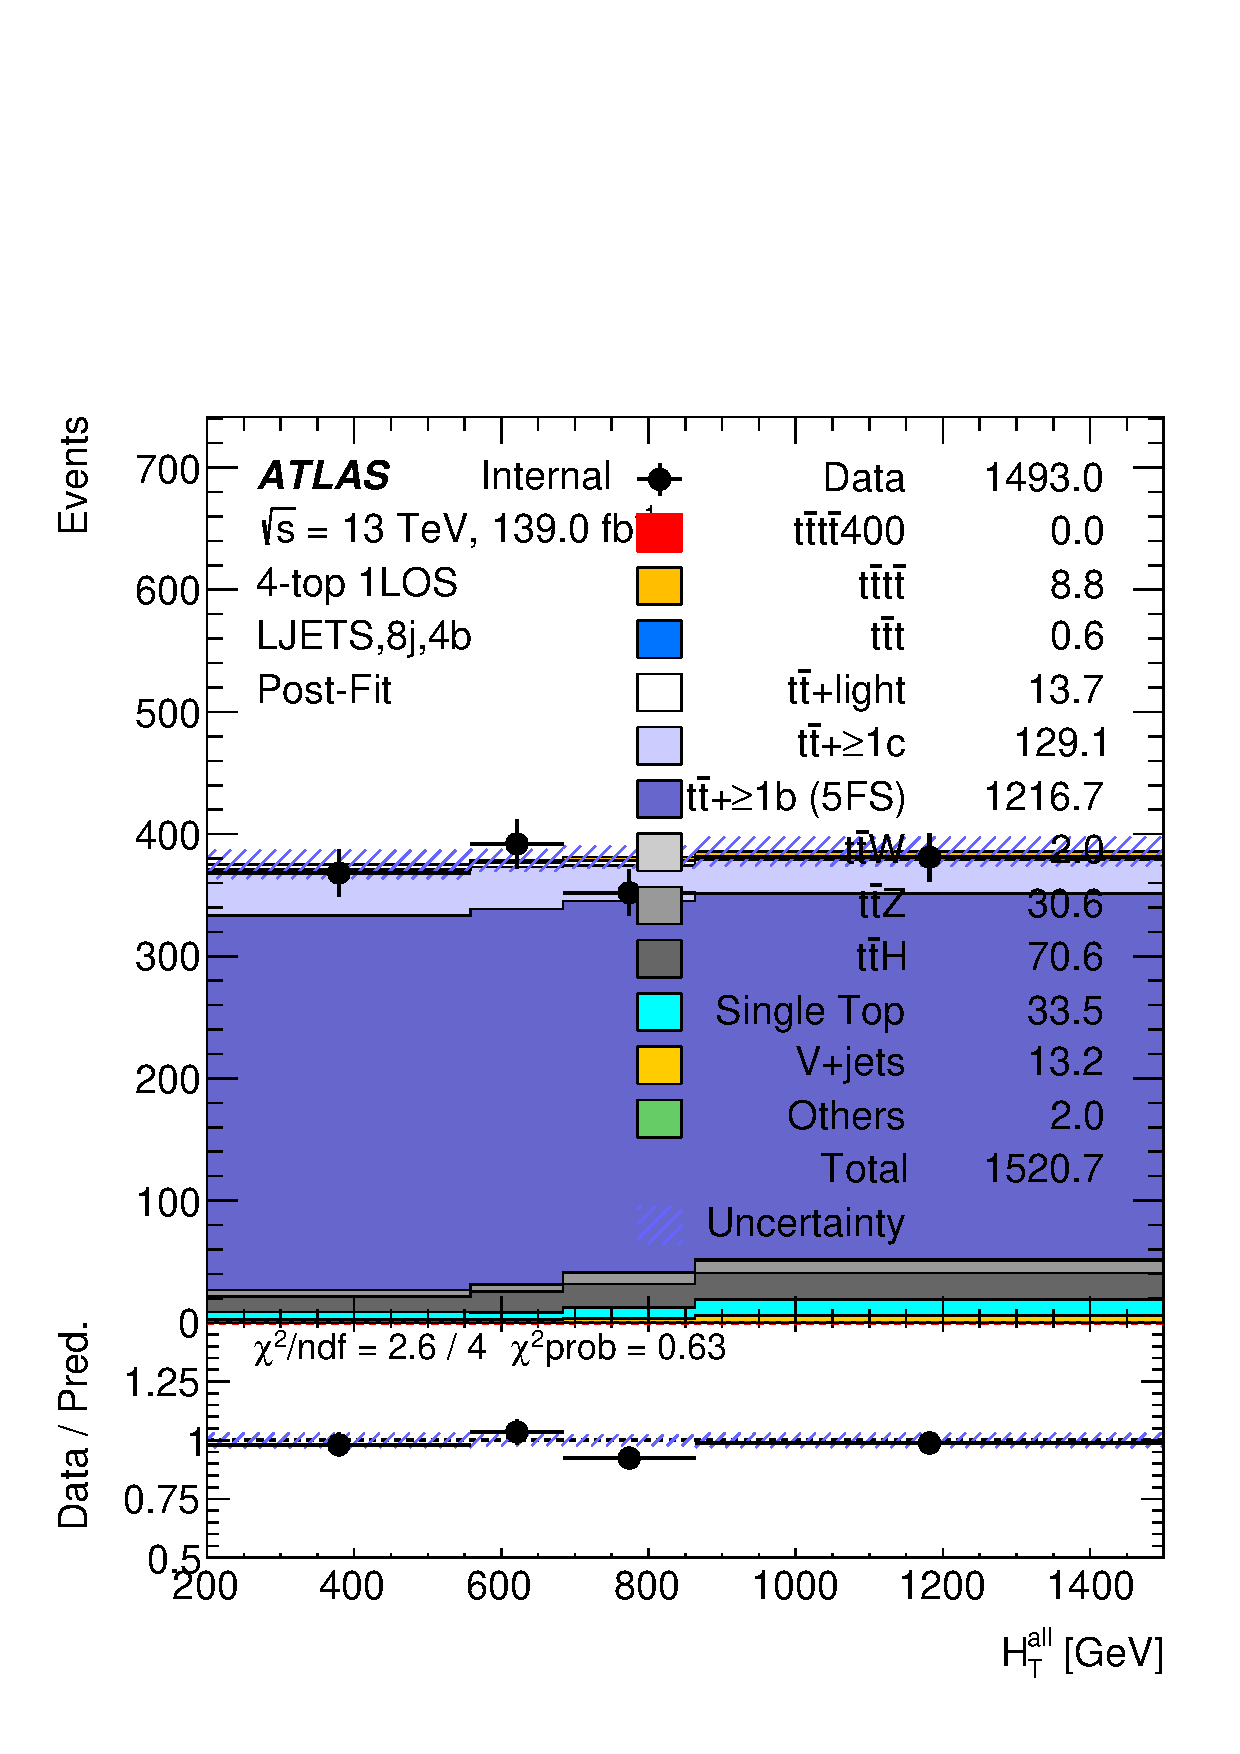
\includegraphics[width=0.23 \textwidth]{figures/fits/GNN/400/all/data/Plots/ljets_8j4b_postFit.pdf} &
        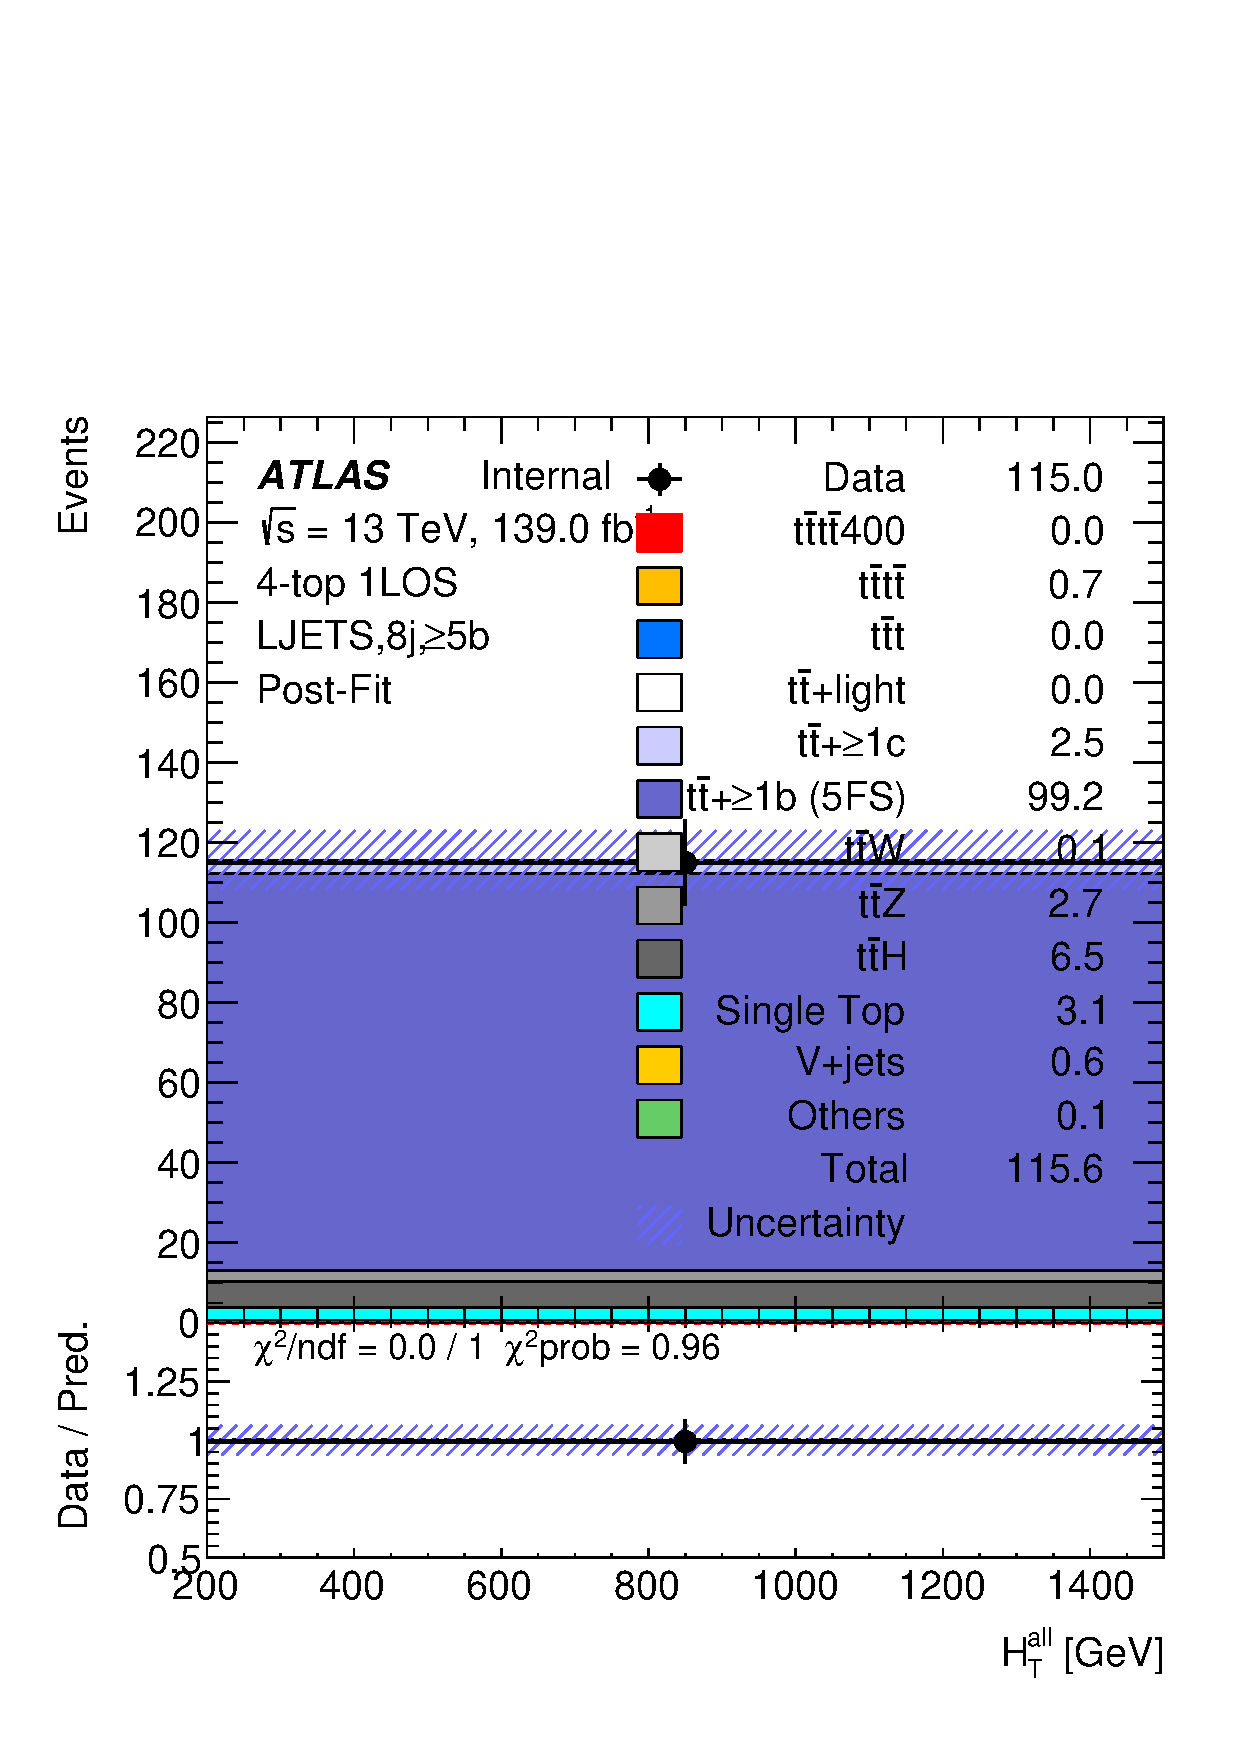
\includegraphics[width=0.23 \textwidth]{figures/fits/GNN/400/all/data/Plots/ljets_8jge5b_postFit.pdf}\\

        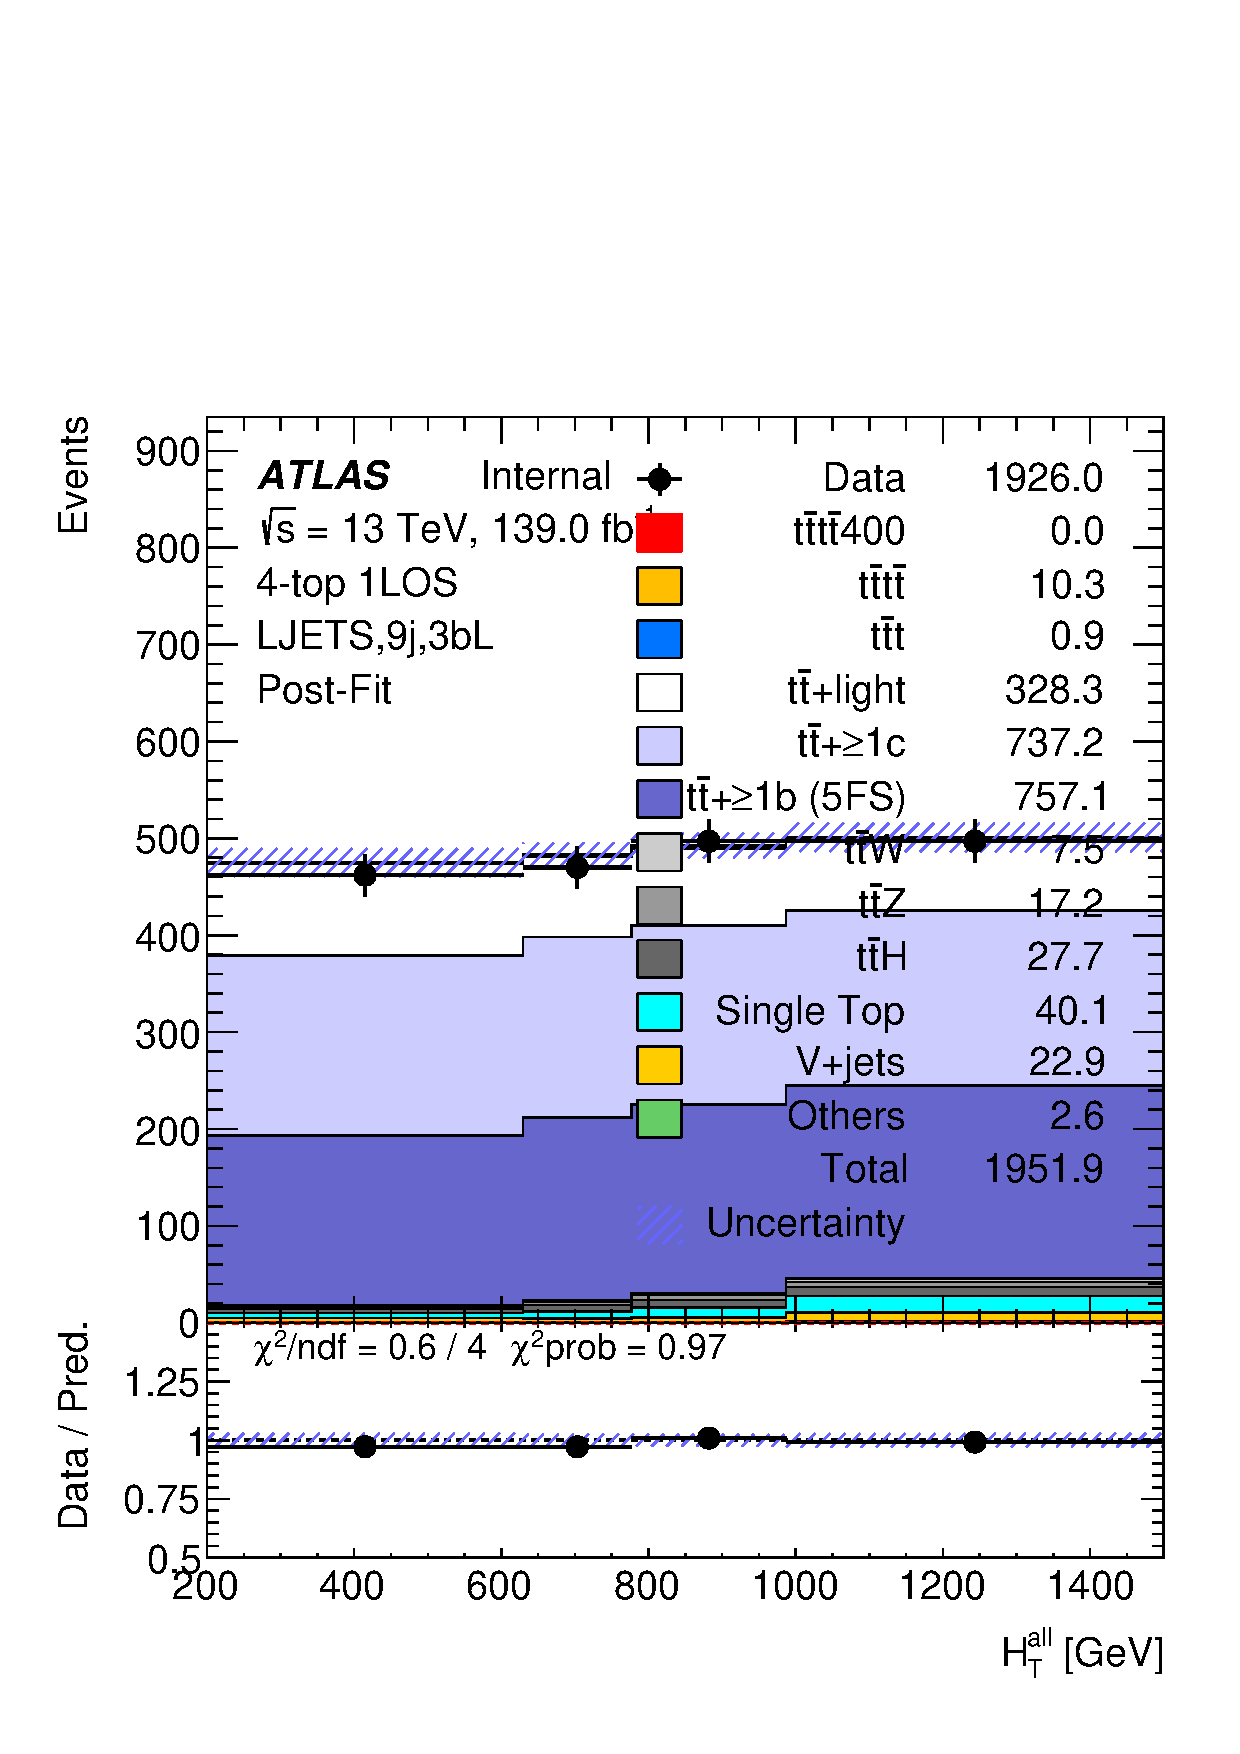
\includegraphics[width=0.23 \textwidth]{figures/fits/GNN/400/all/data/Plots/ljets_9j3bL_postFit.pdf} &
        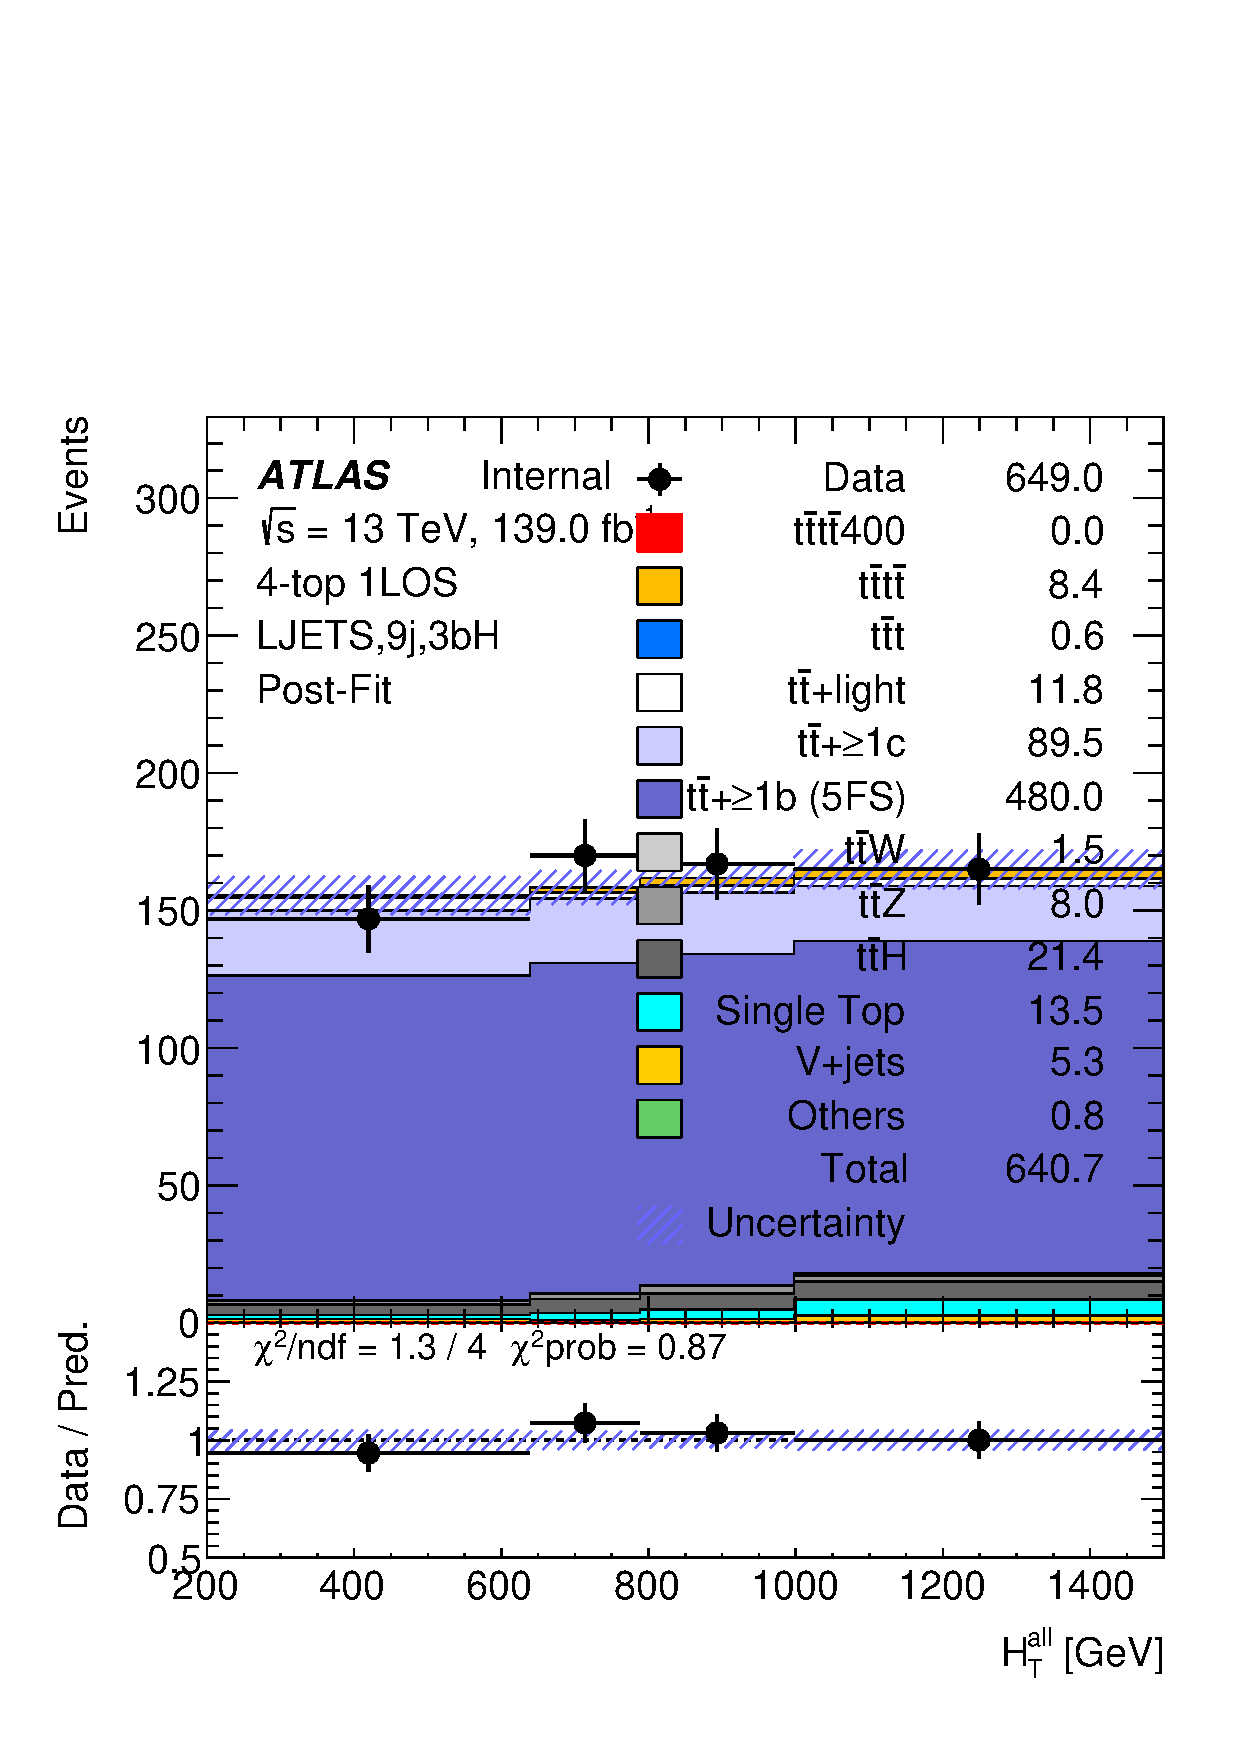
\includegraphics[width=0.23 \textwidth]{figures/fits/GNN/400/all/data/Plots/ljets_9j3bH_postFit.pdf} &
        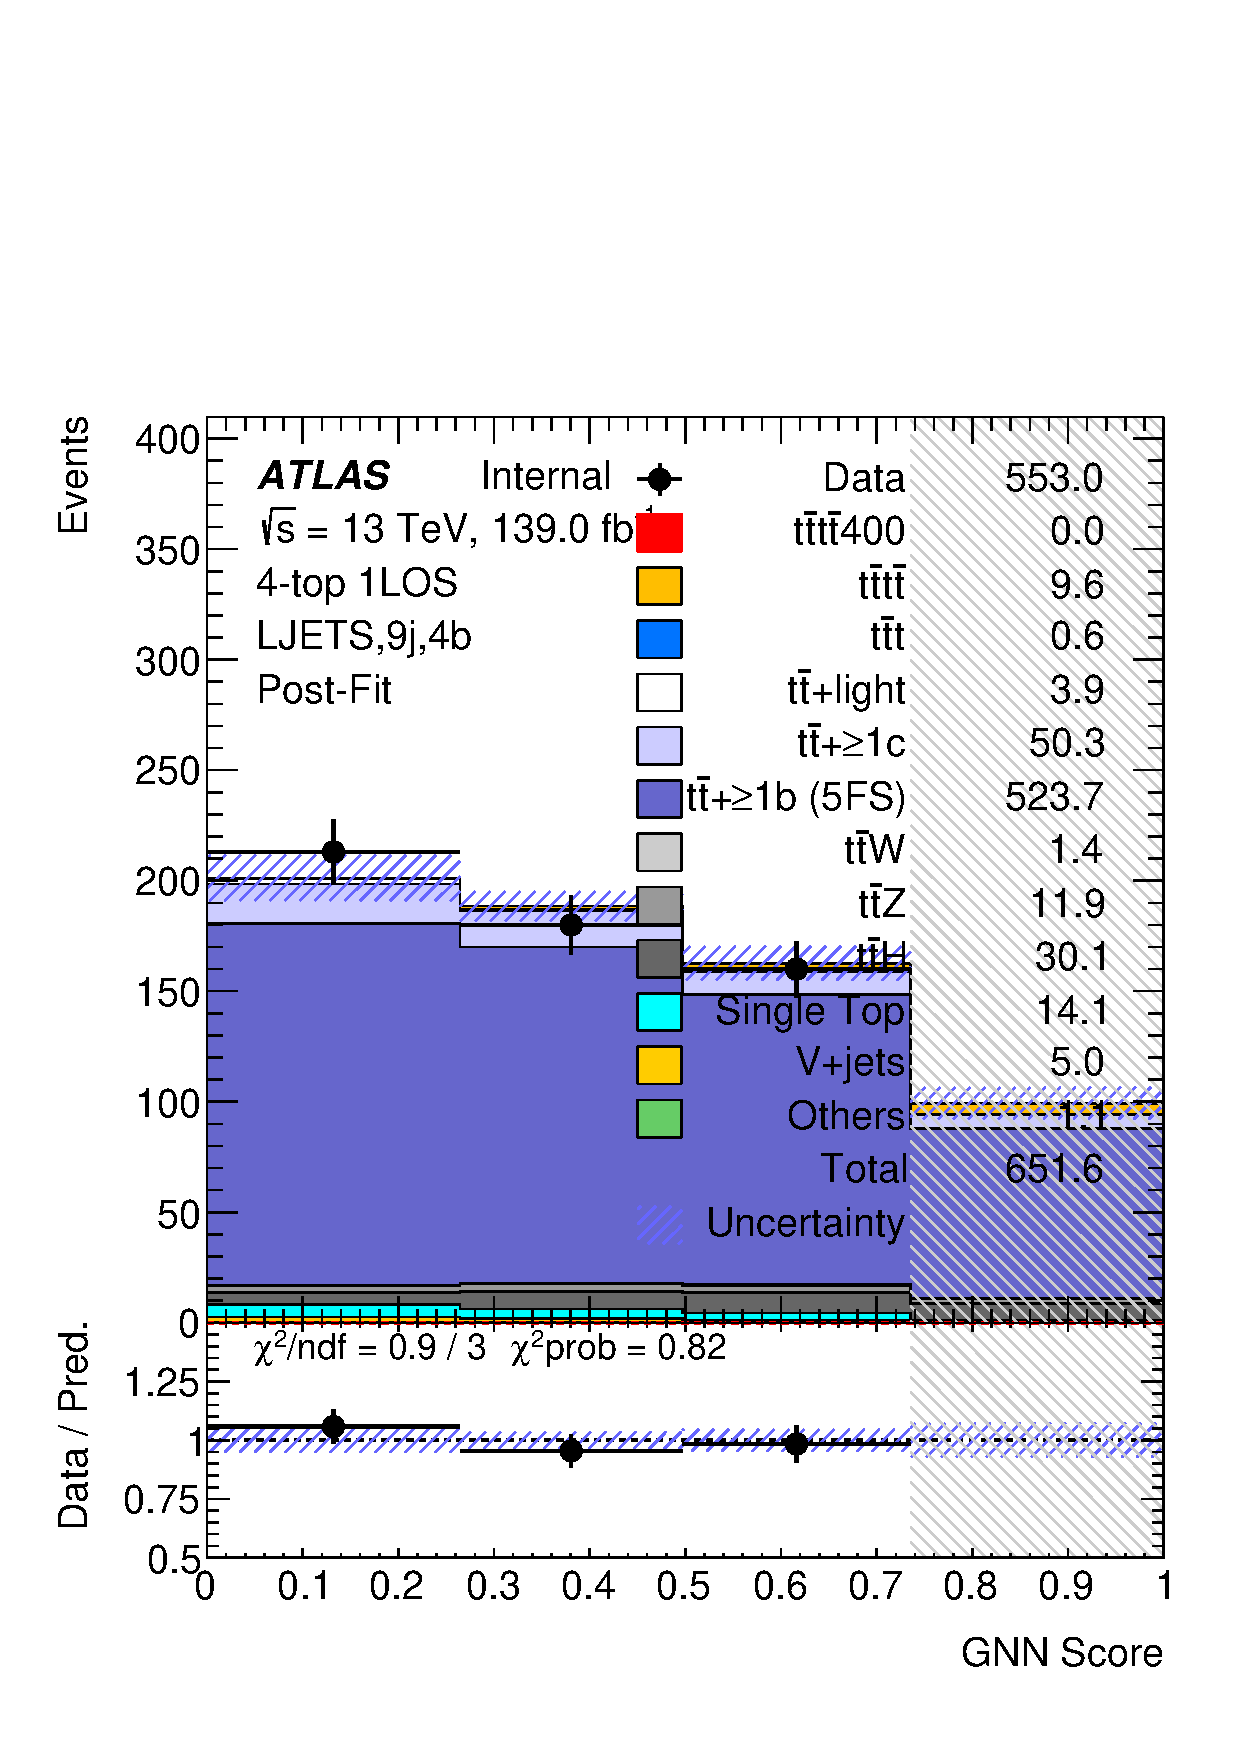
\includegraphics[width=0.23 \textwidth]{figures/fits/GNN/400/all/data/Plots/ljets_9j4b_postFit.pdf} &
        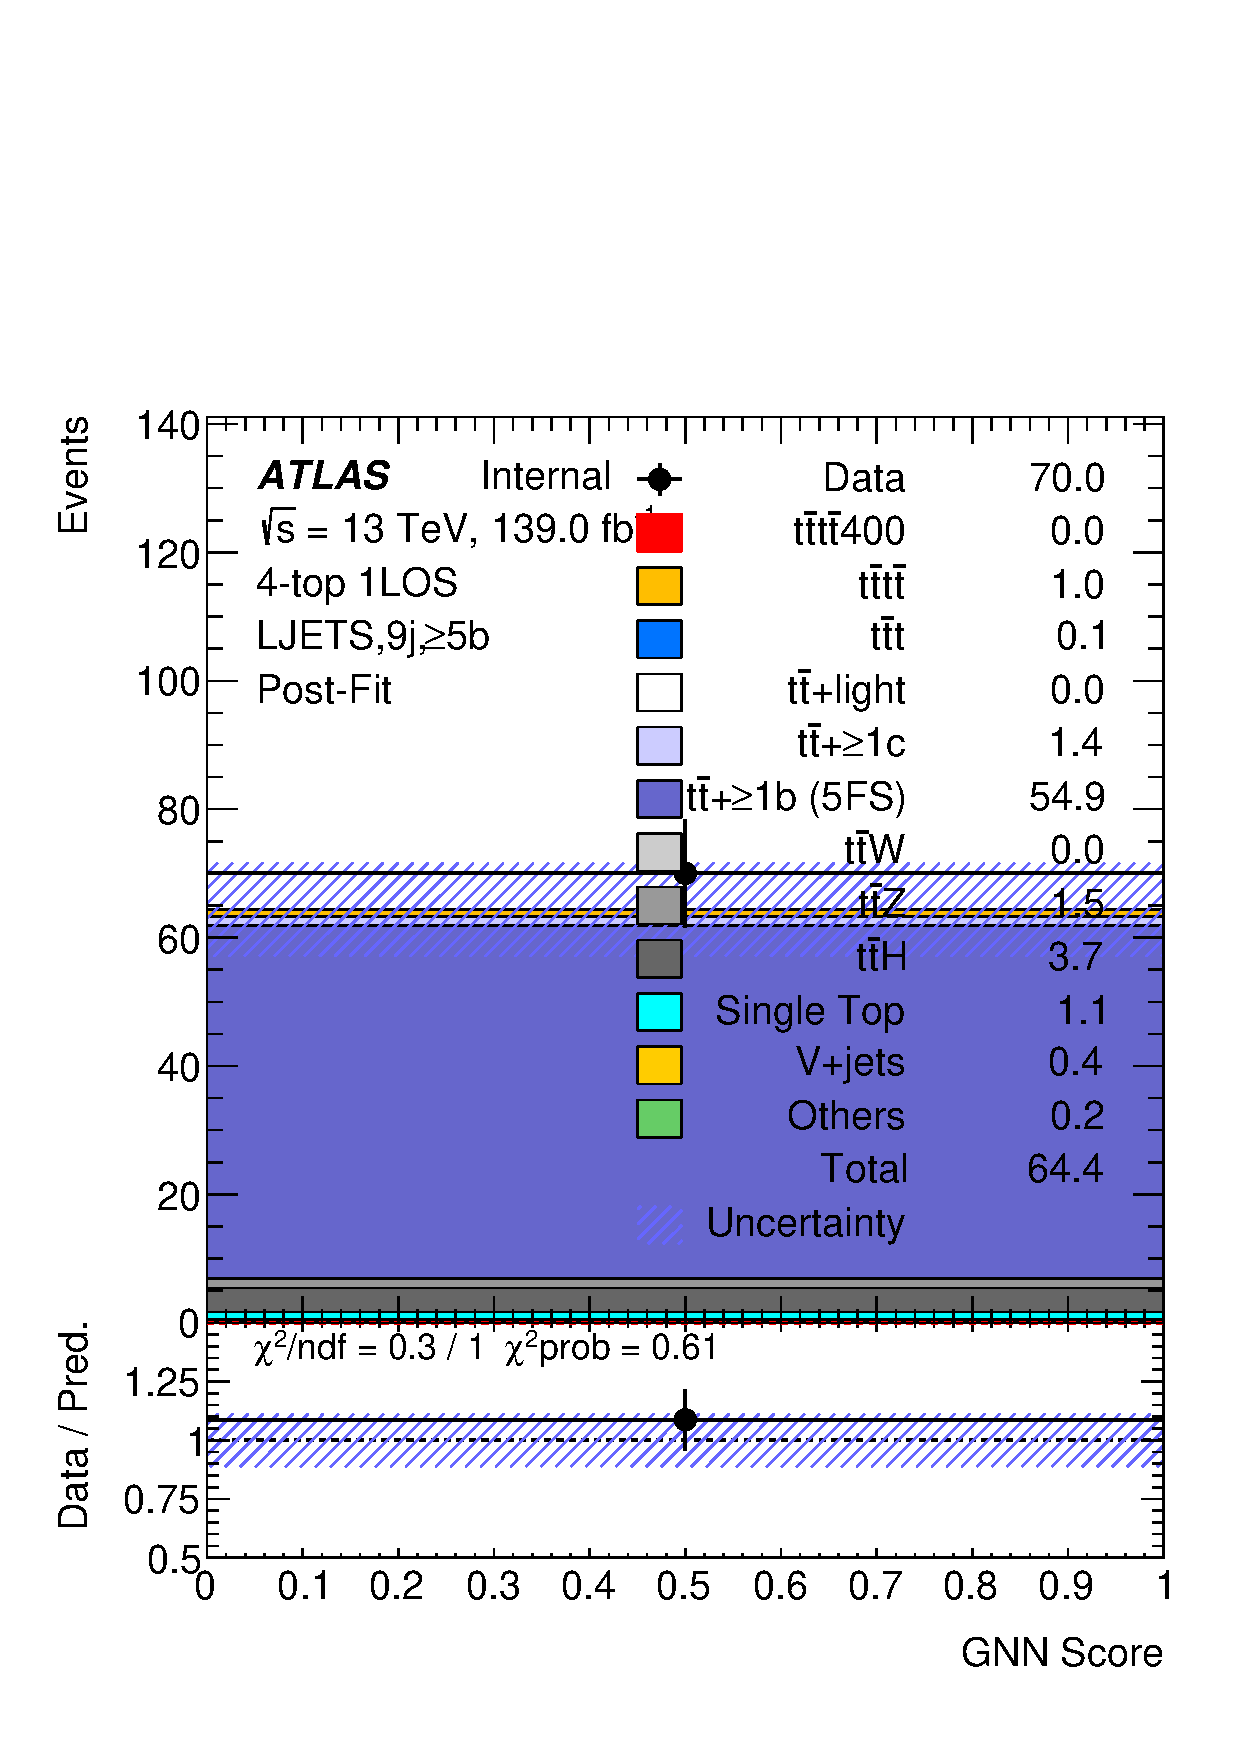
\includegraphics[width=0.23 \textwidth]{figures/fits/GNN/400/all/data/Plots/ljets_9jge5b_postFit.pdf} \\

        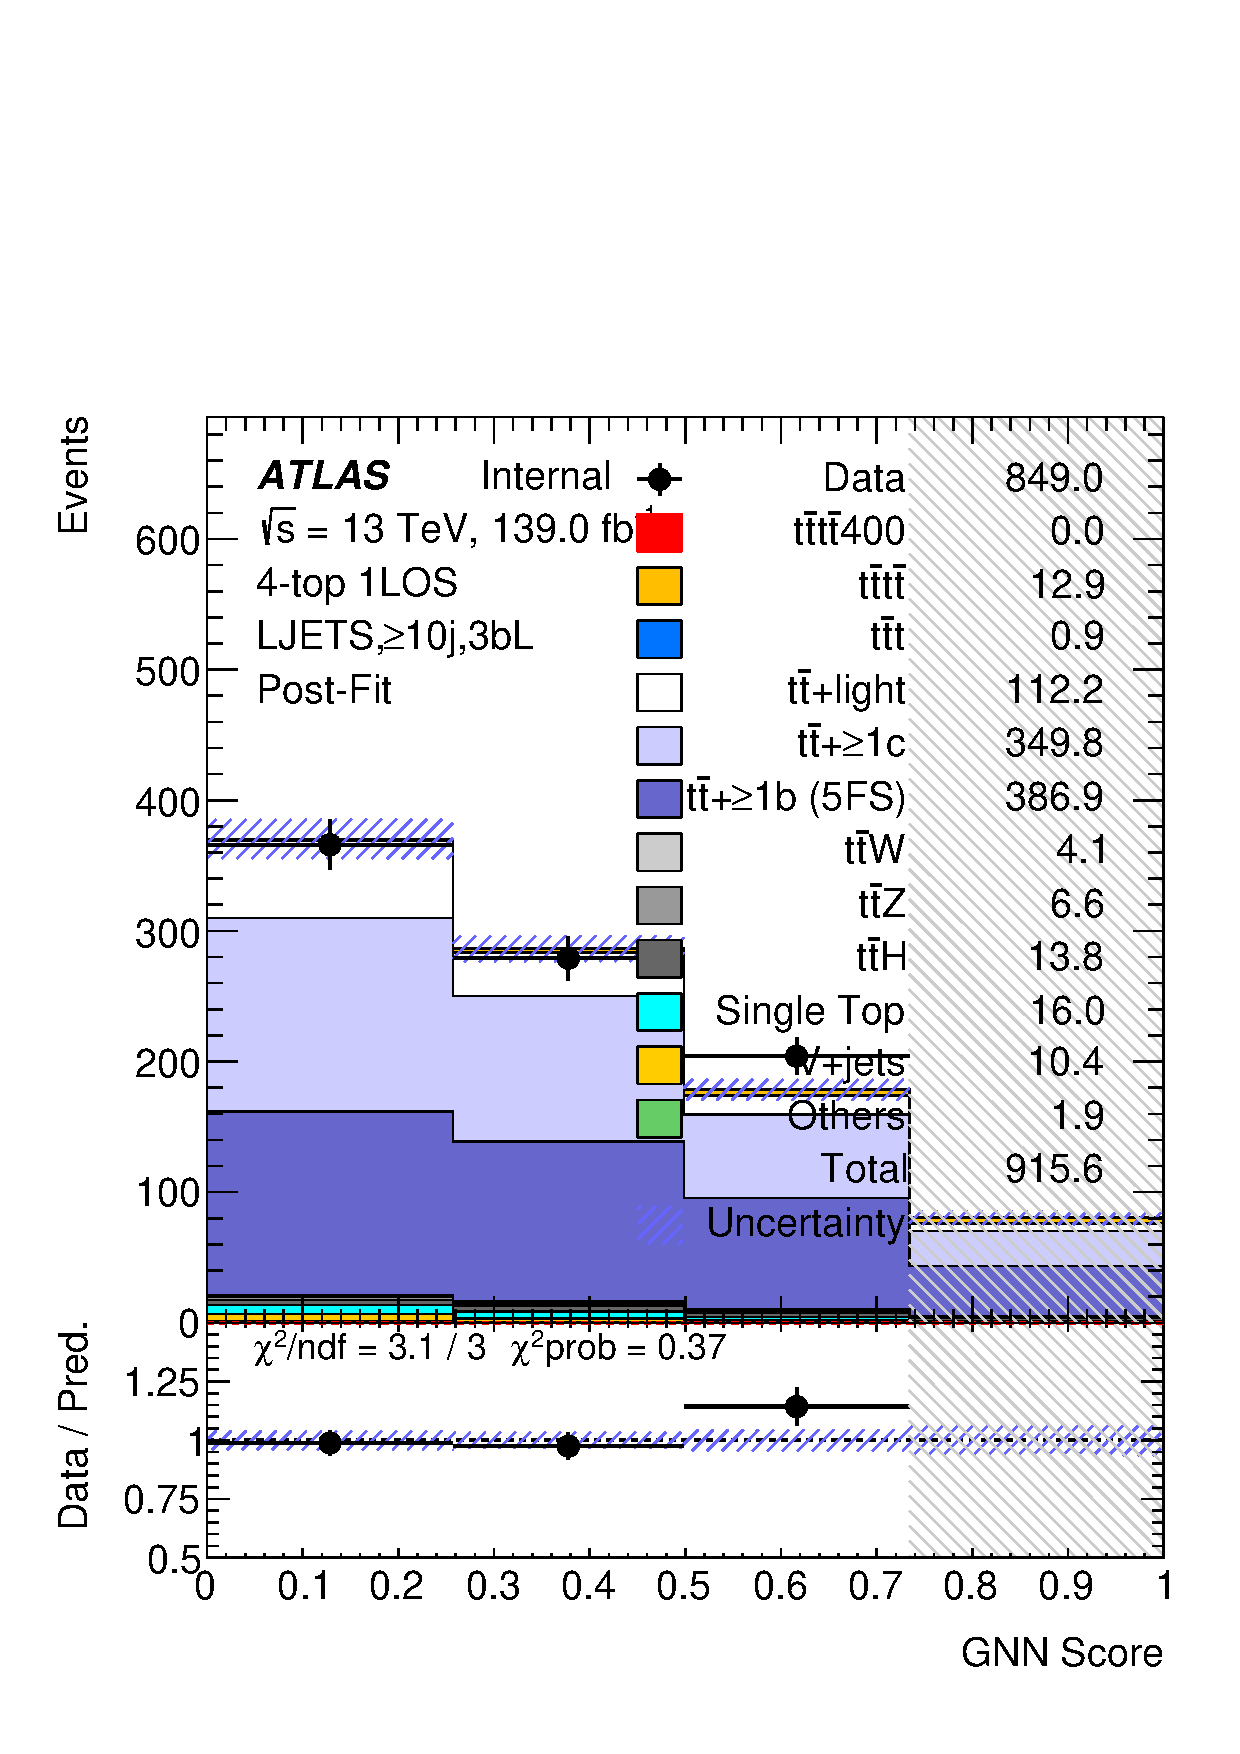
\includegraphics[width=0.23 \textwidth]{figures/fits/GNN/400/all/data/Plots/ljets_ge10j3bL_postFit.pdf} &
        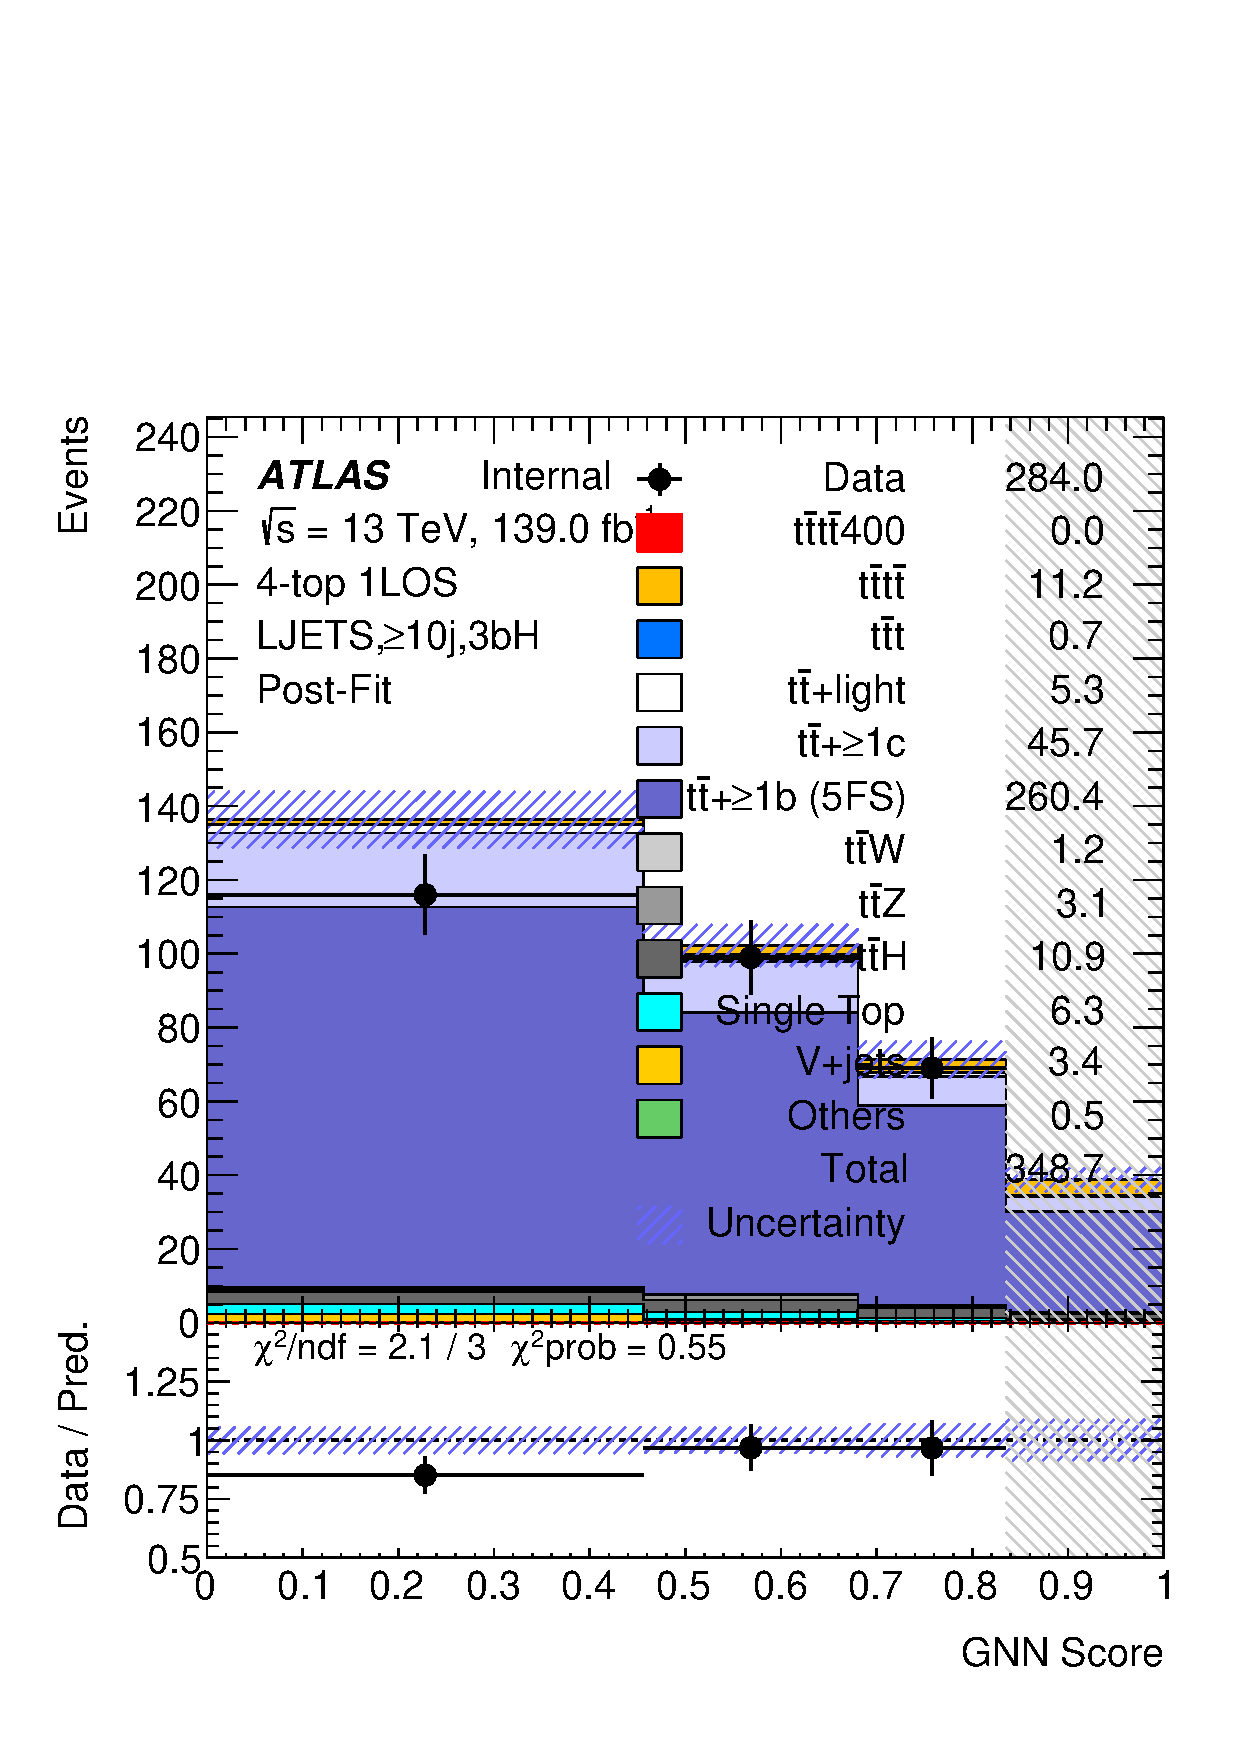
\includegraphics[width=0.23 \textwidth]{figures/fits/GNN/400/all/data/Plots/ljets_ge10j3bH_postFit.pdf} &
        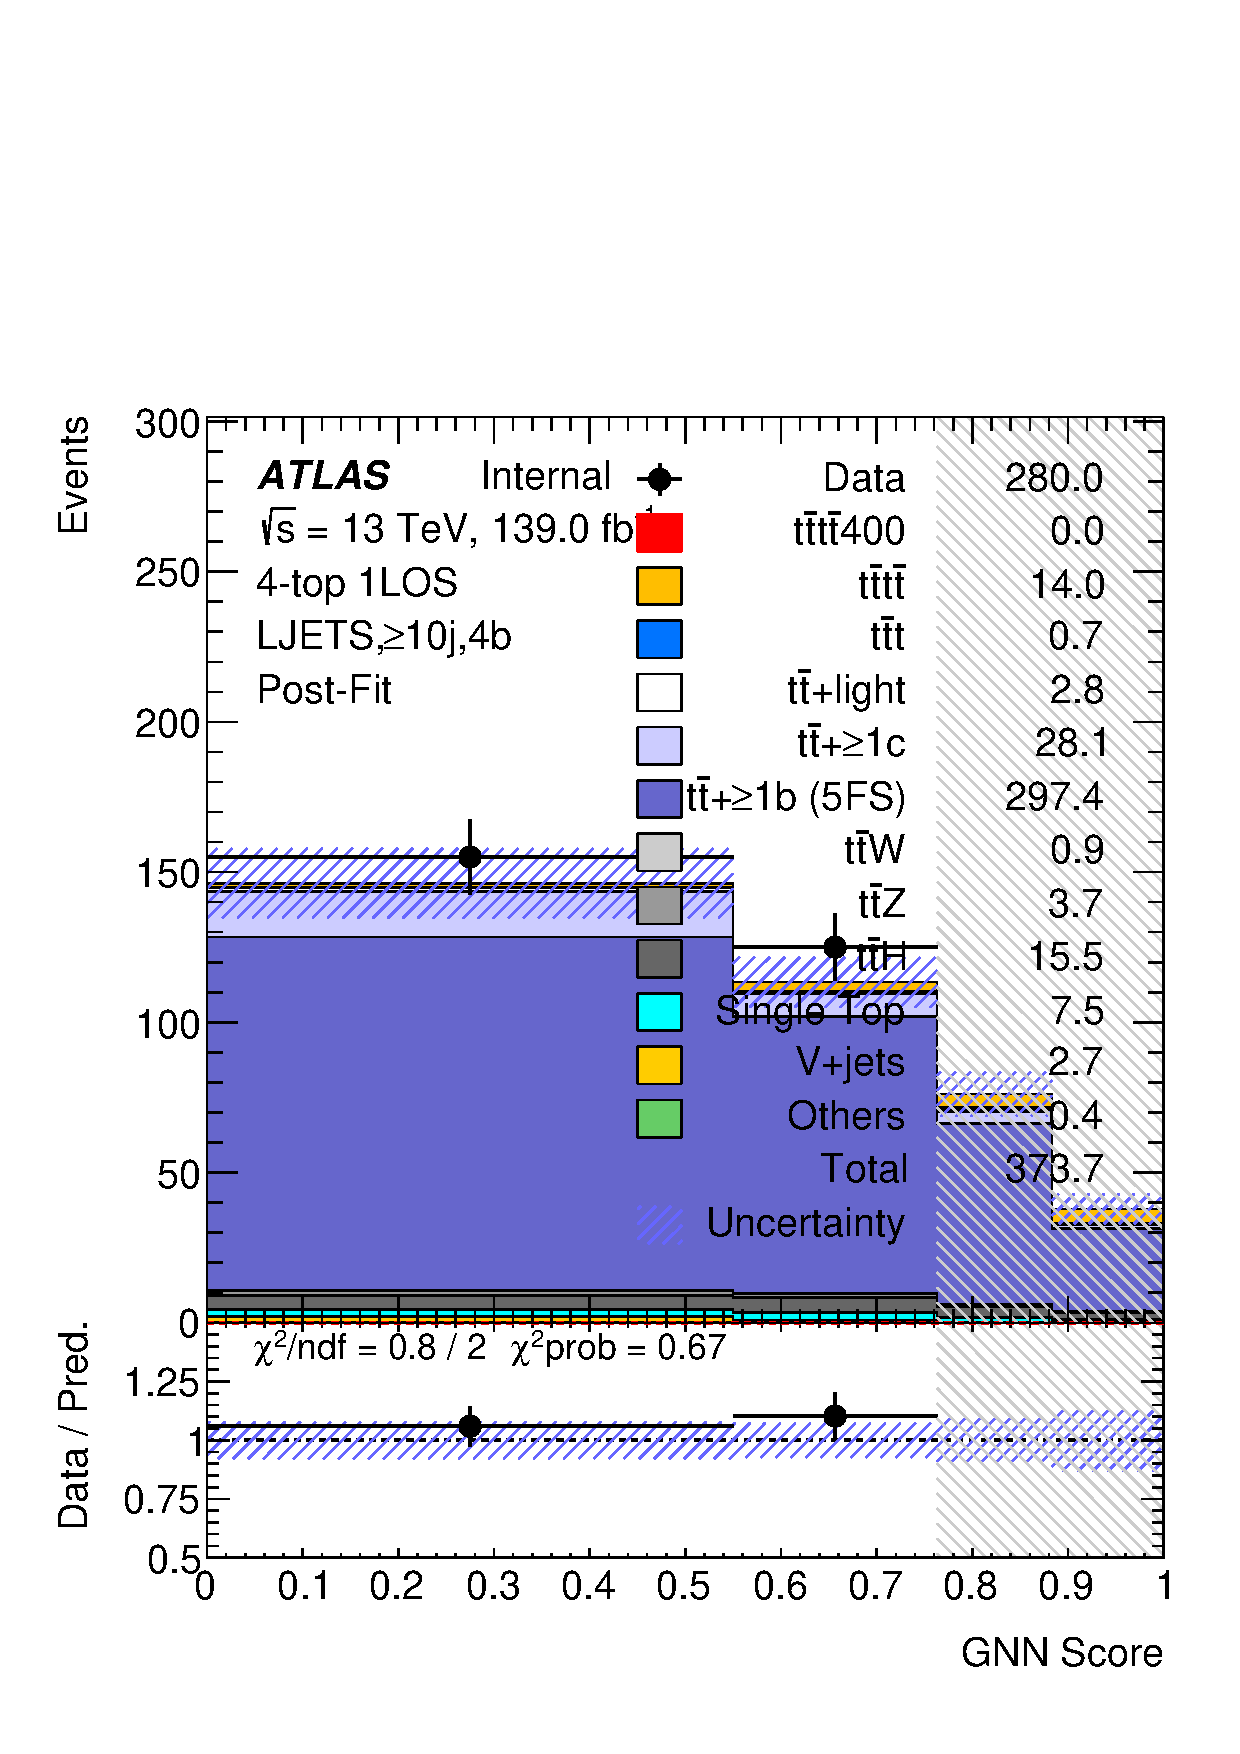
\includegraphics[width=0.23 \textwidth]{figures/fits/GNN/400/all/data/Plots/ljets_ge10j4b_postFit.pdf} &
        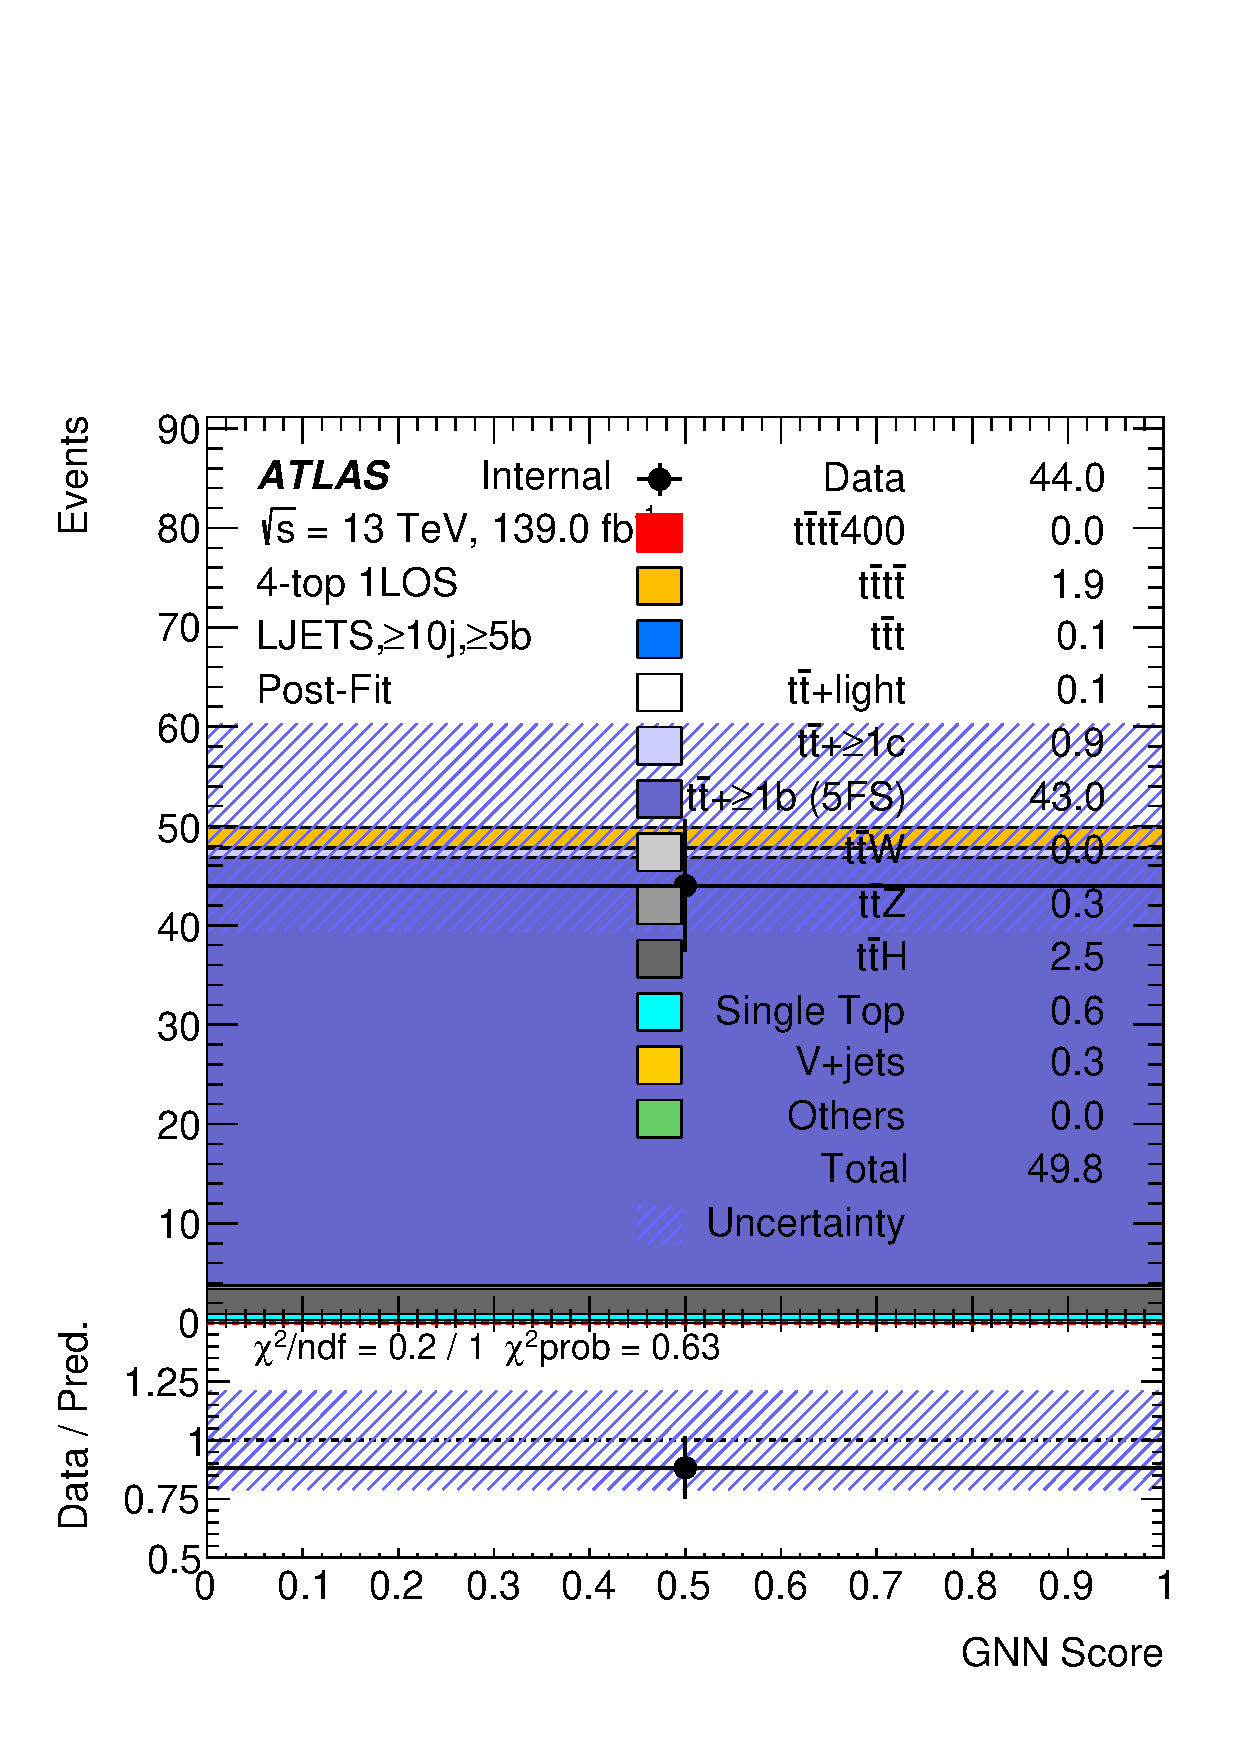
\includegraphics[width=0.23 \textwidth]{figures/fits/GNN/400/all/data/Plots/ljets_ge10jge5b_postFit.pdf} \\
        \end{tabular}
        \caption{\label{fig:Postfit_Yields_1L}Post-fit distributions for 1L regions associated with different signal and background samples, compared with data yields for mH = 400 GeV. The fit is done using all regions (1L+2L).}
\end{center}
\end{figure}

\begin{figure}[htbp!]
        \begin{center} \setlength{\tabcolsep}{2.5pt}\footnotesize
        \begin{tabular}{ccc}
        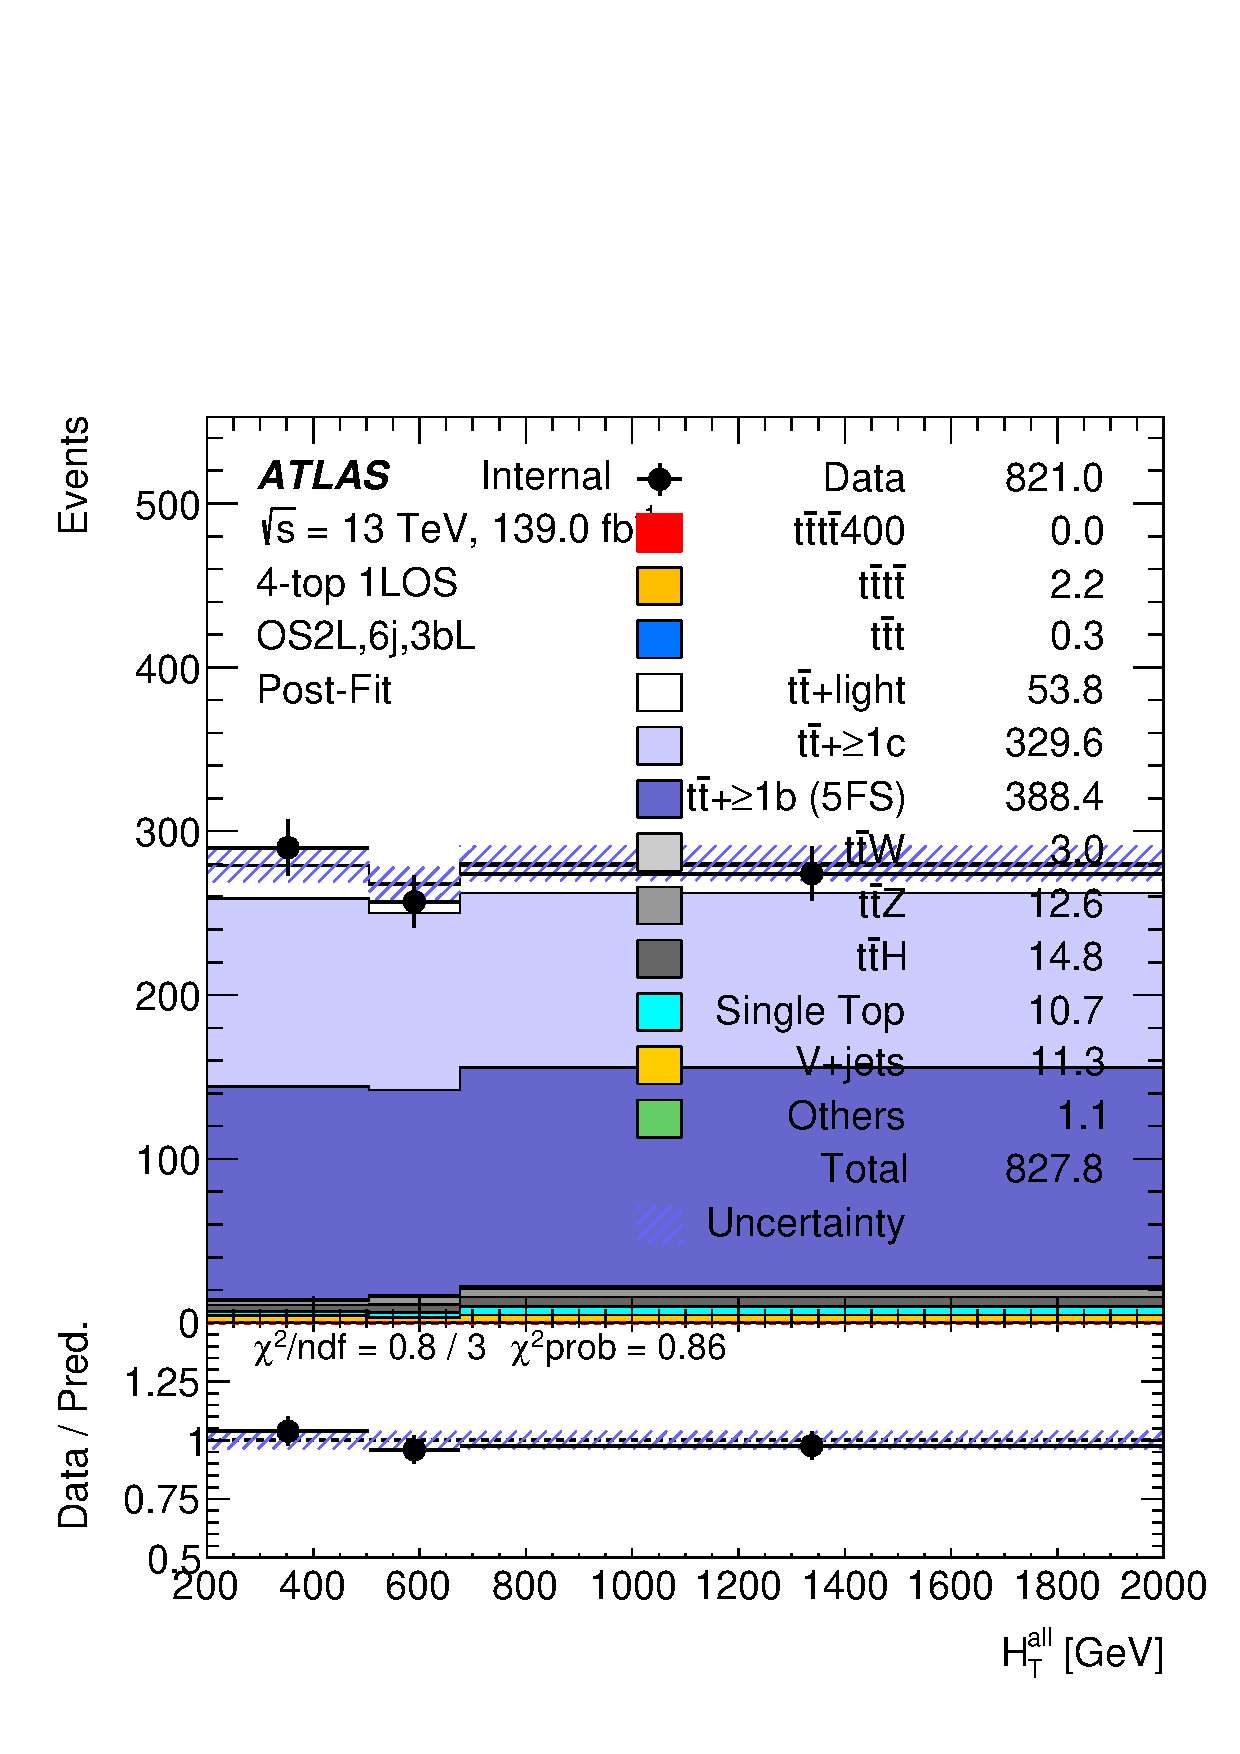
\includegraphics[width=0.31 \textwidth]{figures/fits/GNN/400/all/data/Plots/os2l_6j3bL_postFit.pdf} &
        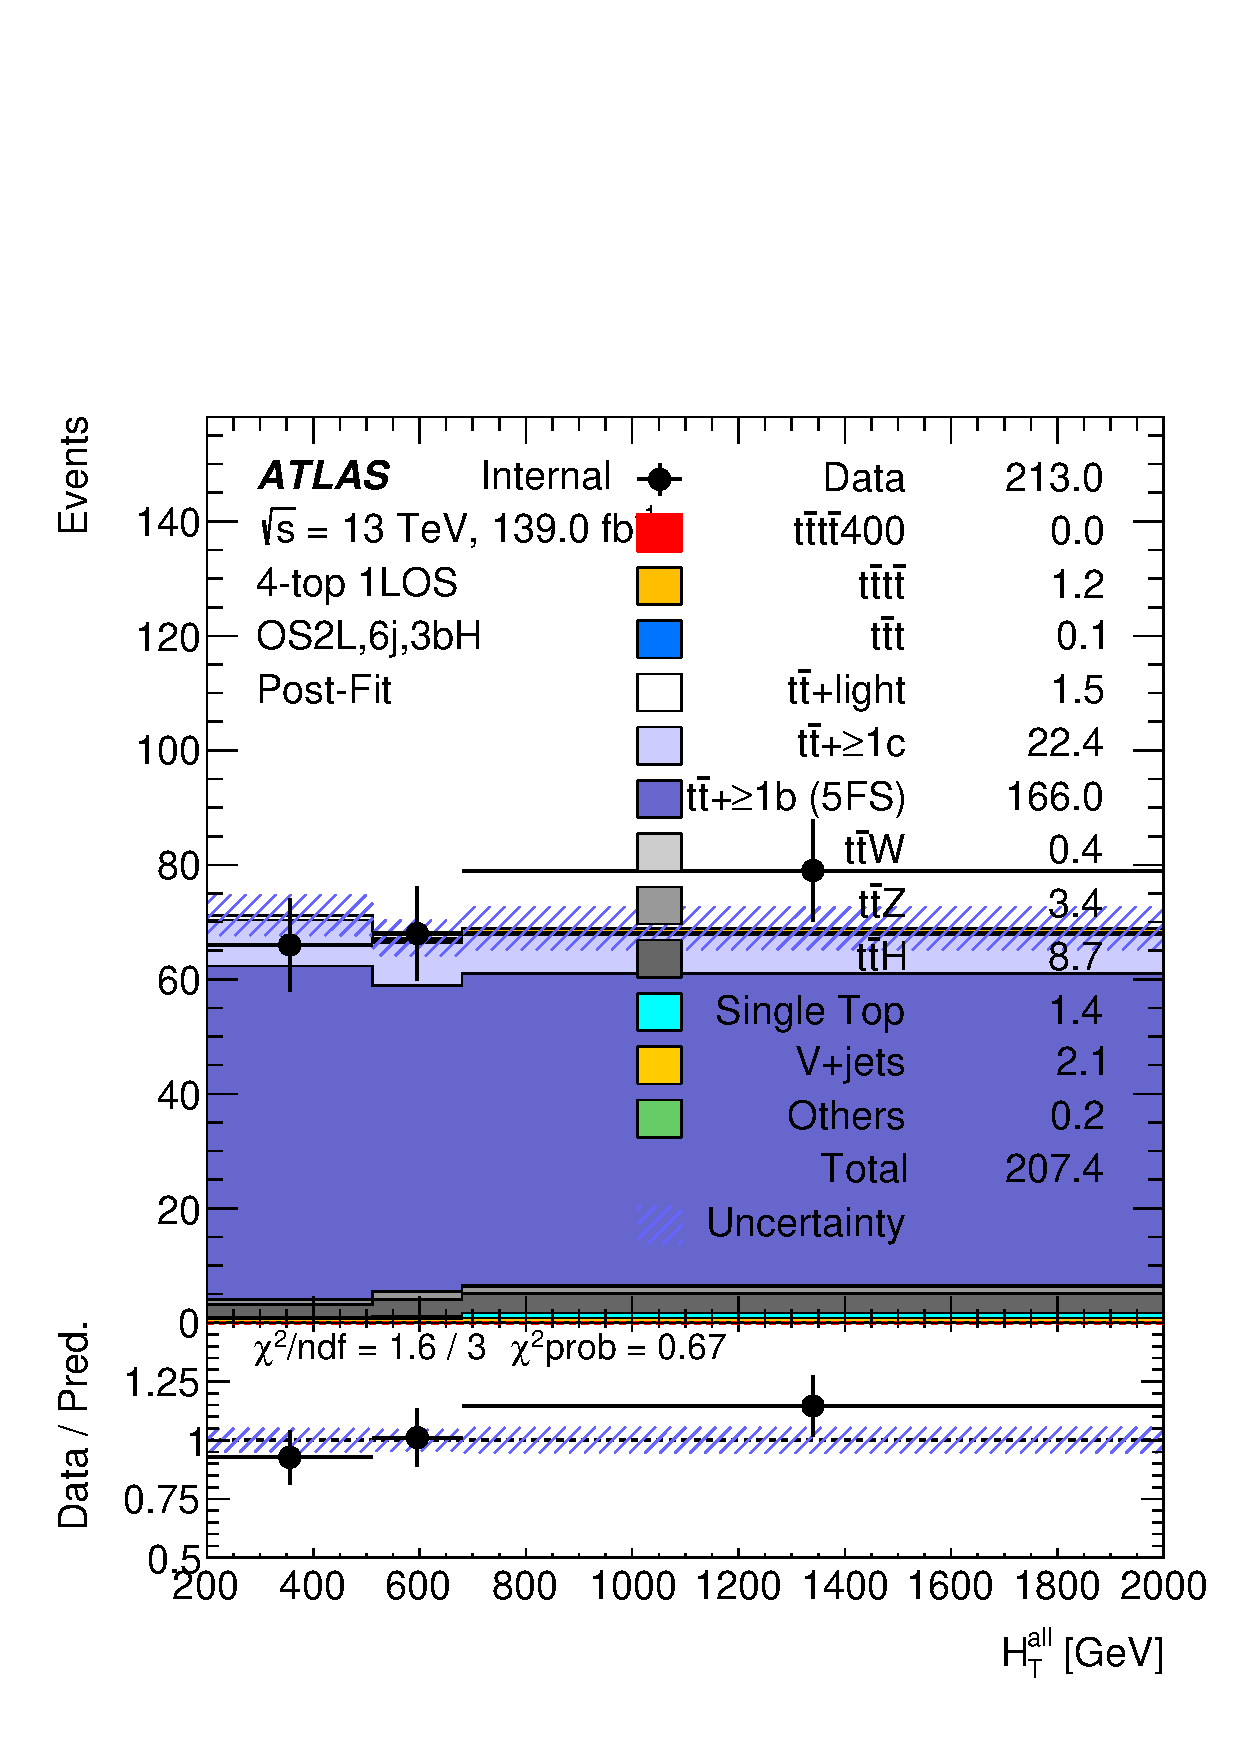
\includegraphics[width=0.31 \textwidth]{figures/fits/GNN/400/all/data/Plots/os2l_6j3bH_postFit.pdf} &
        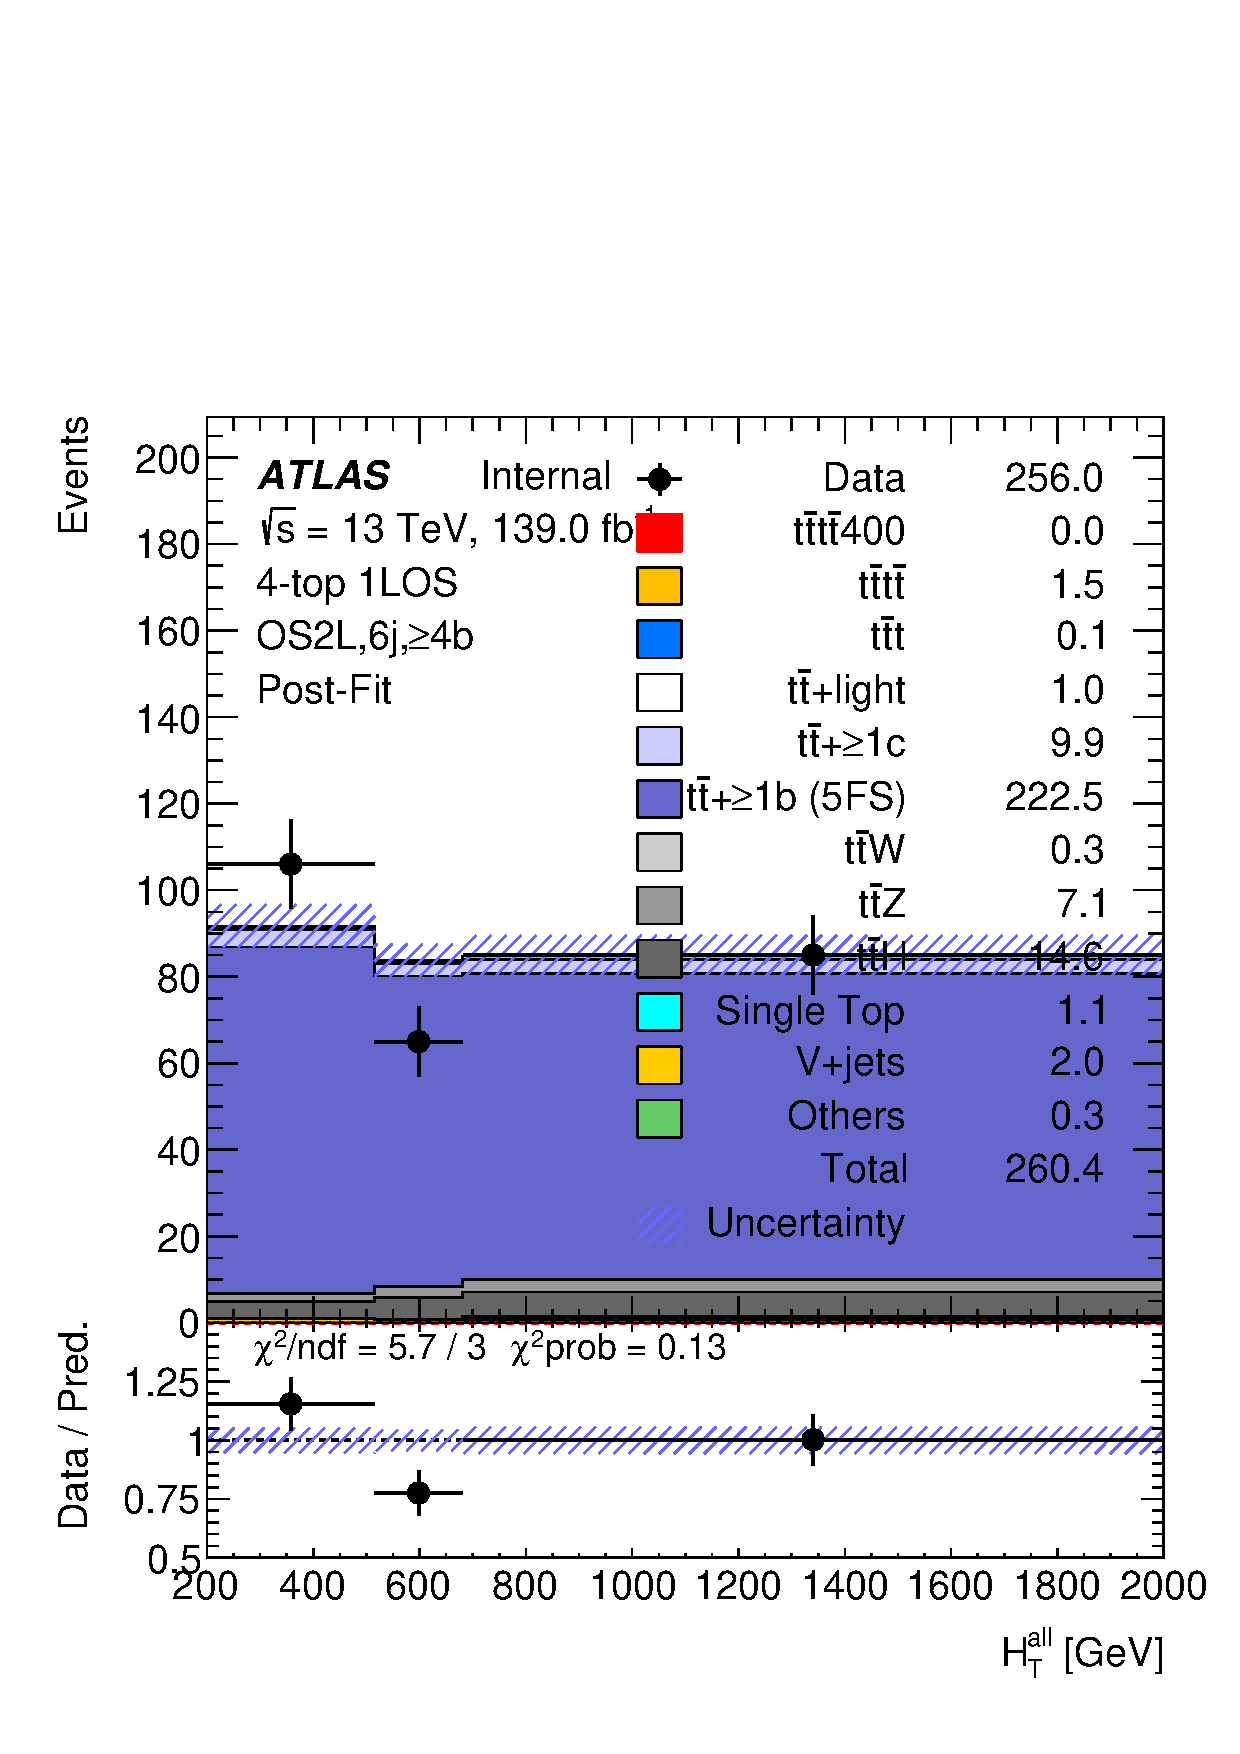
\includegraphics[width=0.31 \textwidth]{figures/fits/GNN/400/all/data/Plots/os2l_6jge4b_postFit.pdf} \\

        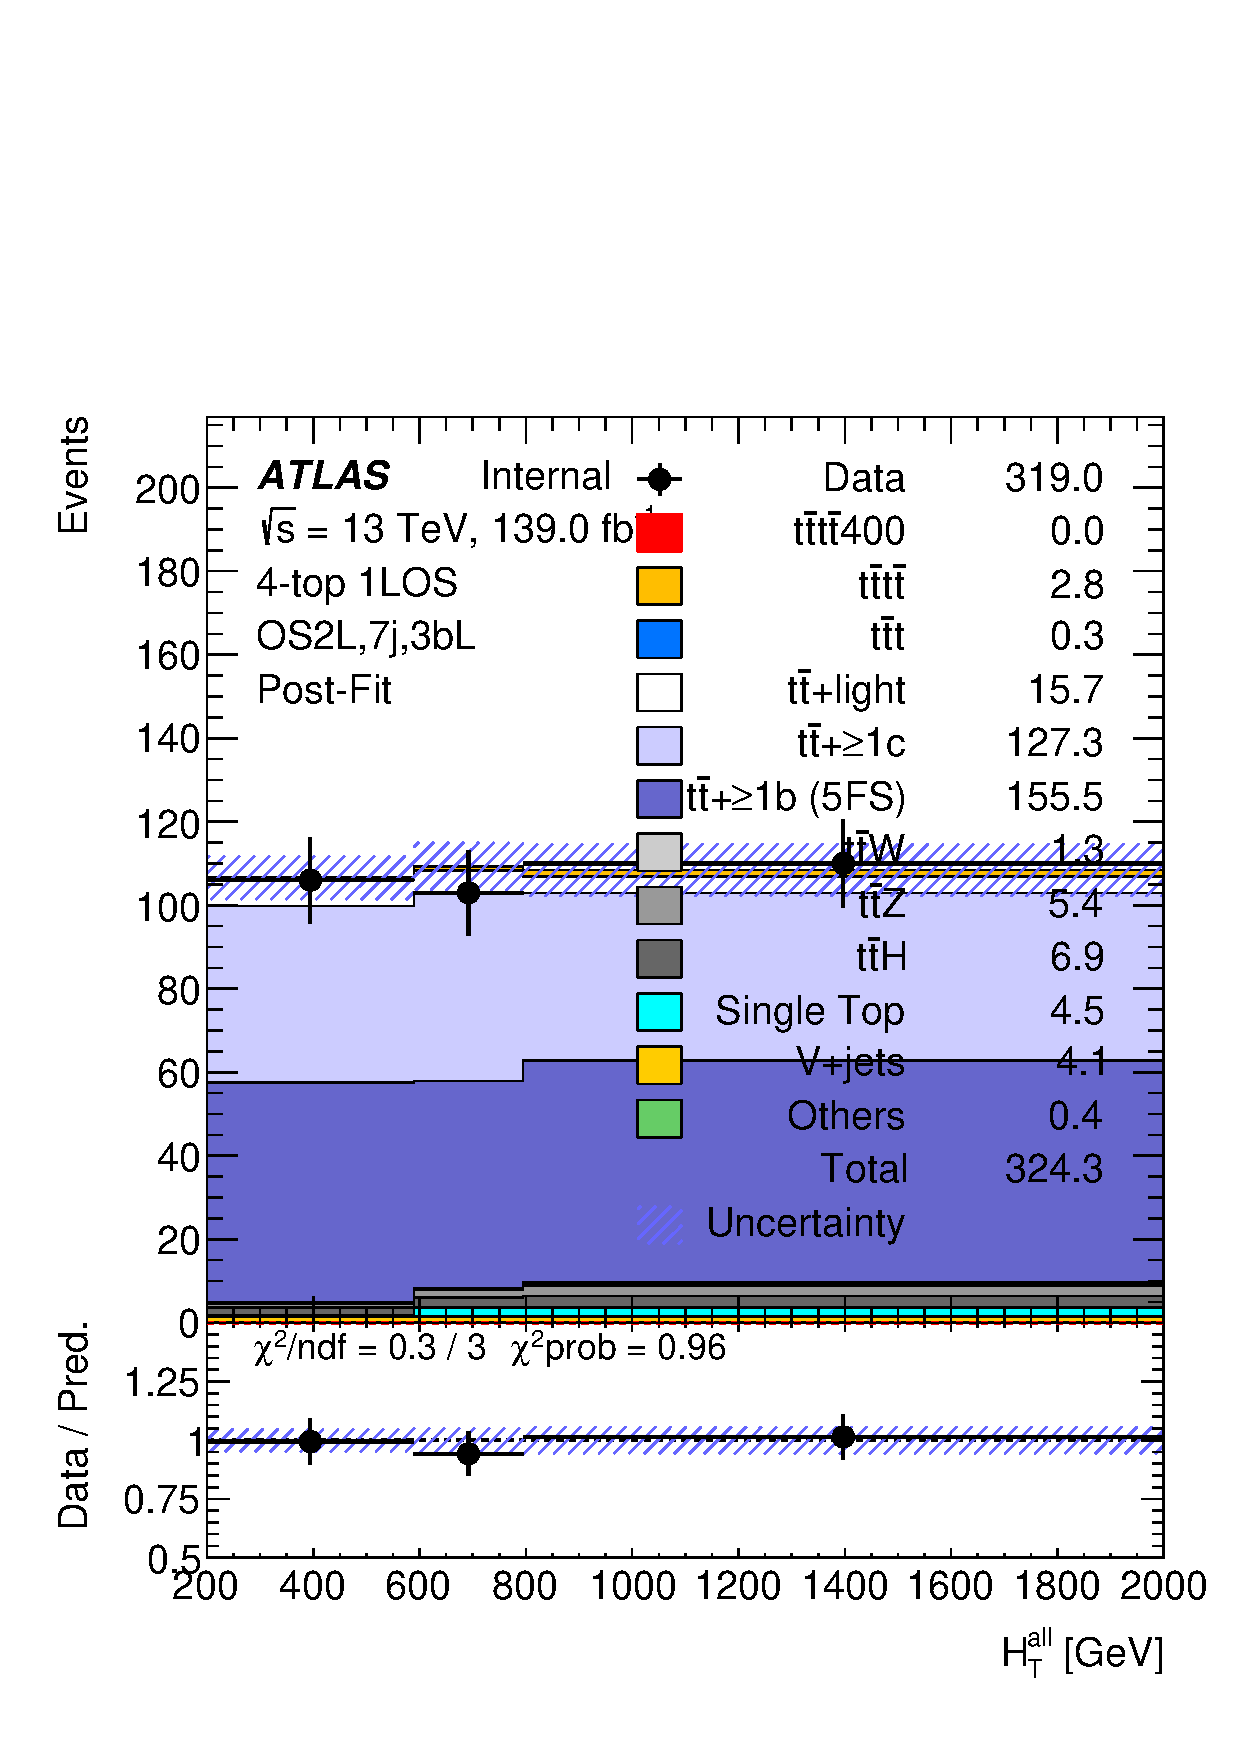
\includegraphics[width=0.31 \textwidth]{figures/fits/GNN/400/all/data/Plots/os2l_7j3bL_postFit.pdf} &
        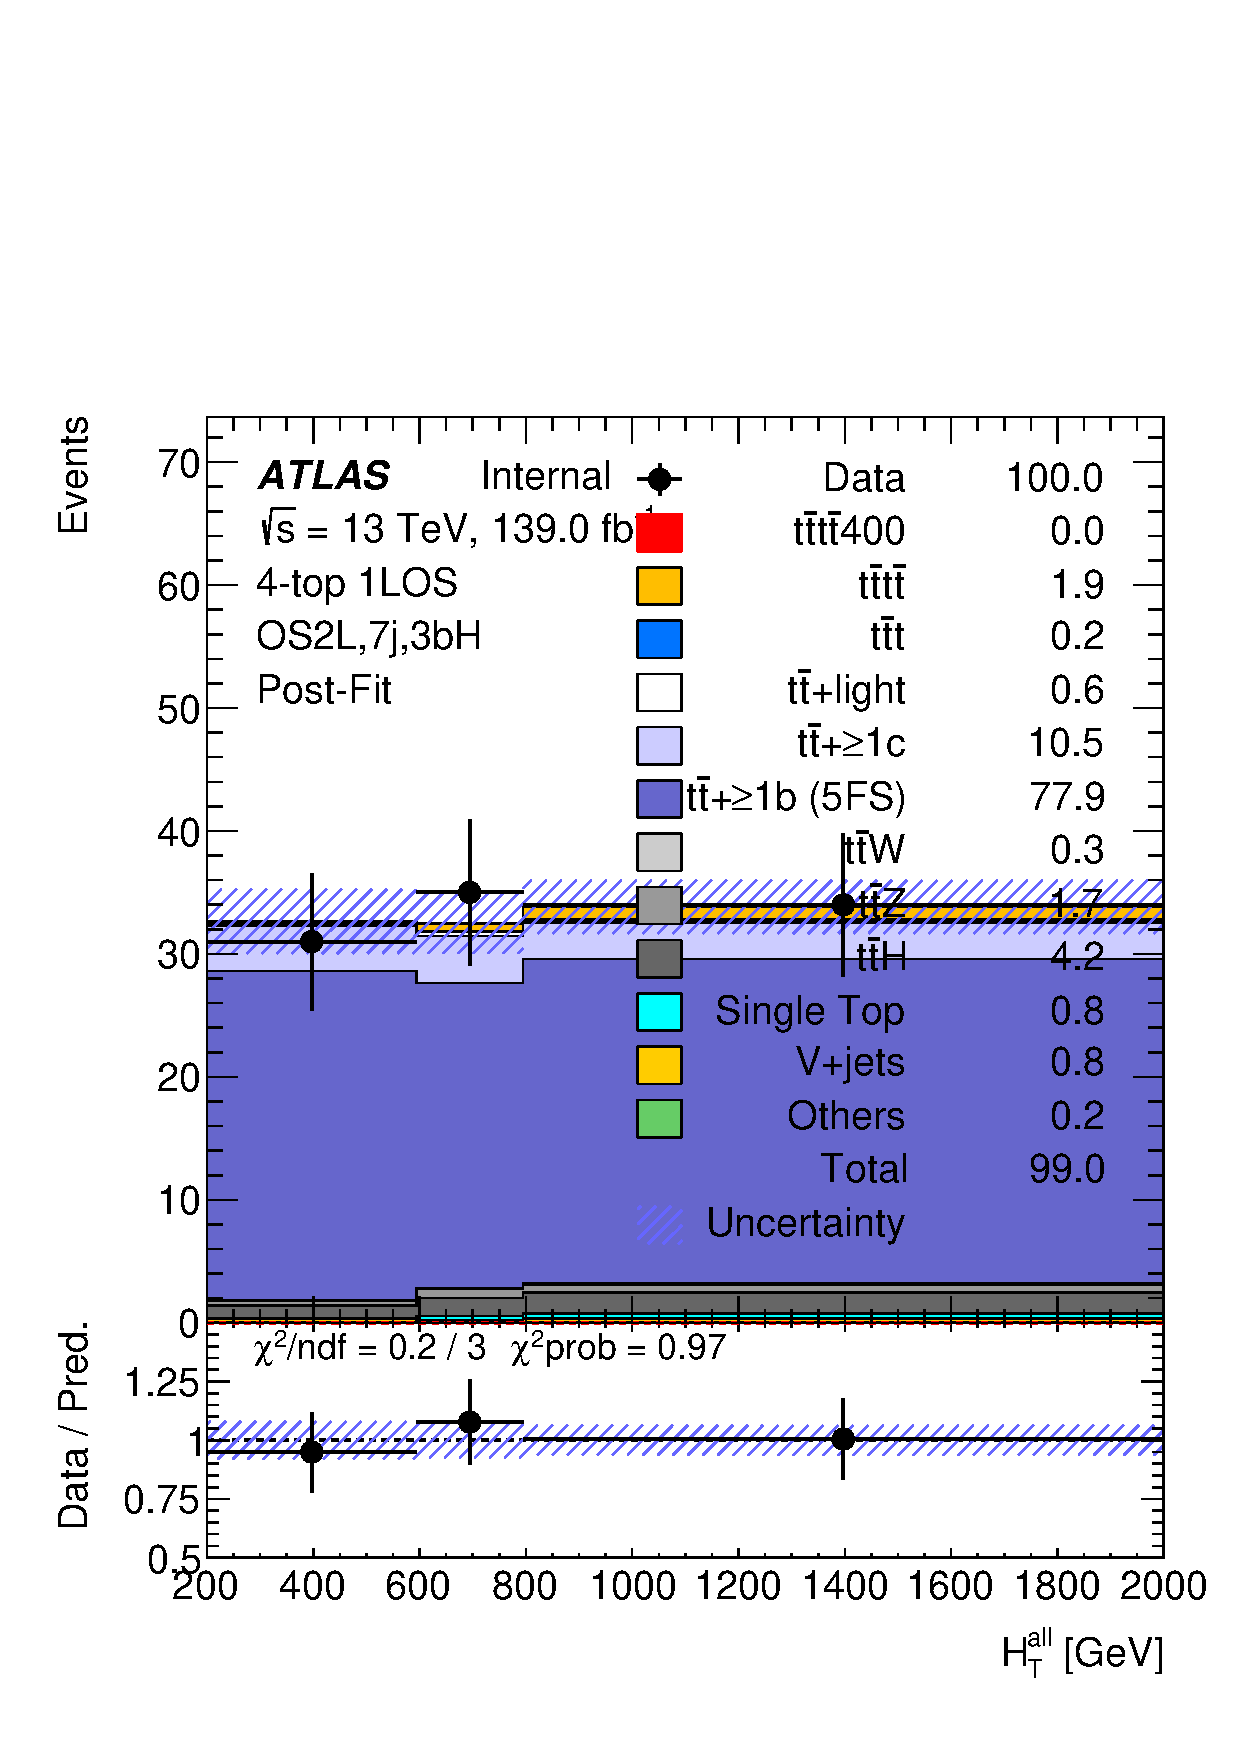
\includegraphics[width=0.31 \textwidth]{figures/fits/GNN/400/all/data/Plots/os2l_7j3bH_postFit.pdf} &
        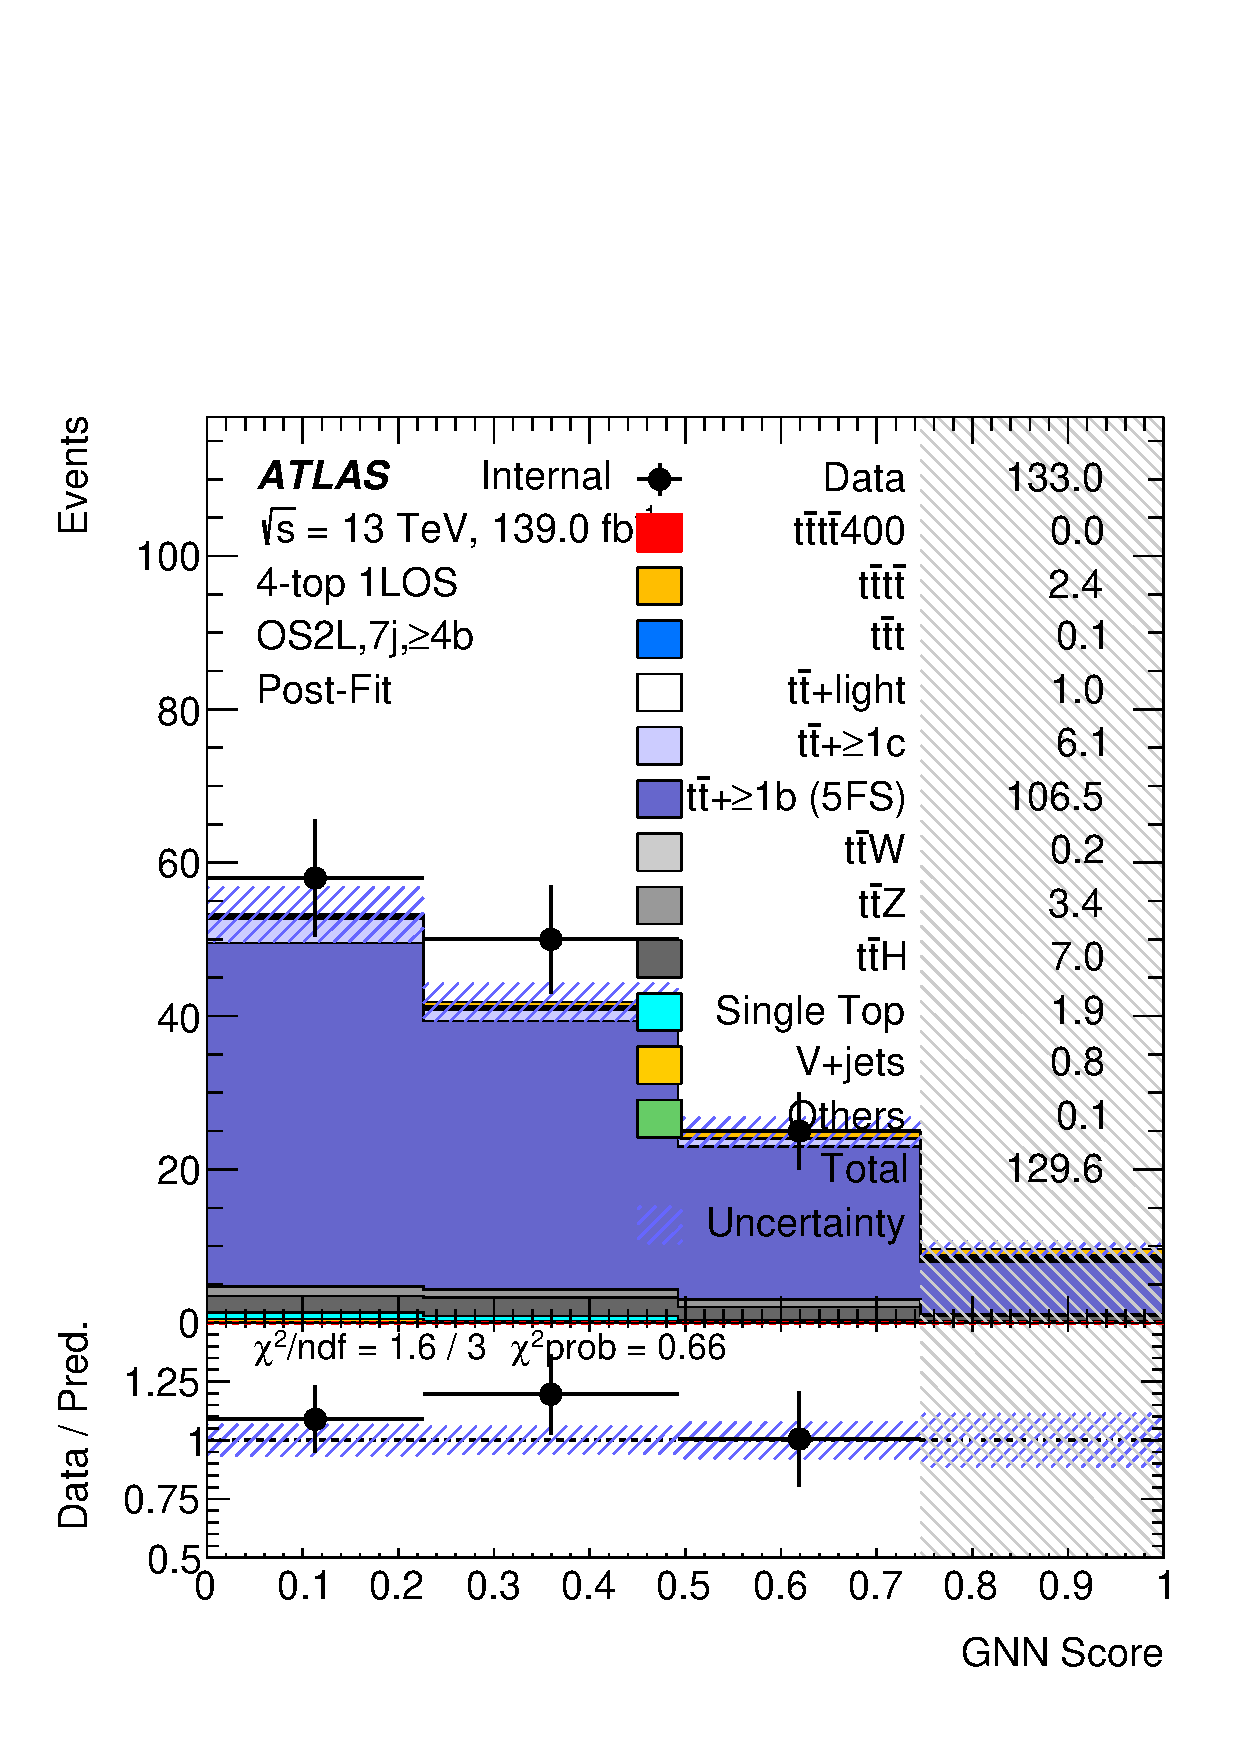
\includegraphics[width=0.31 \textwidth]{figures/fits/GNN/400/all/data/Plots/os2l_7jge4b_postFit.pdf} \\

        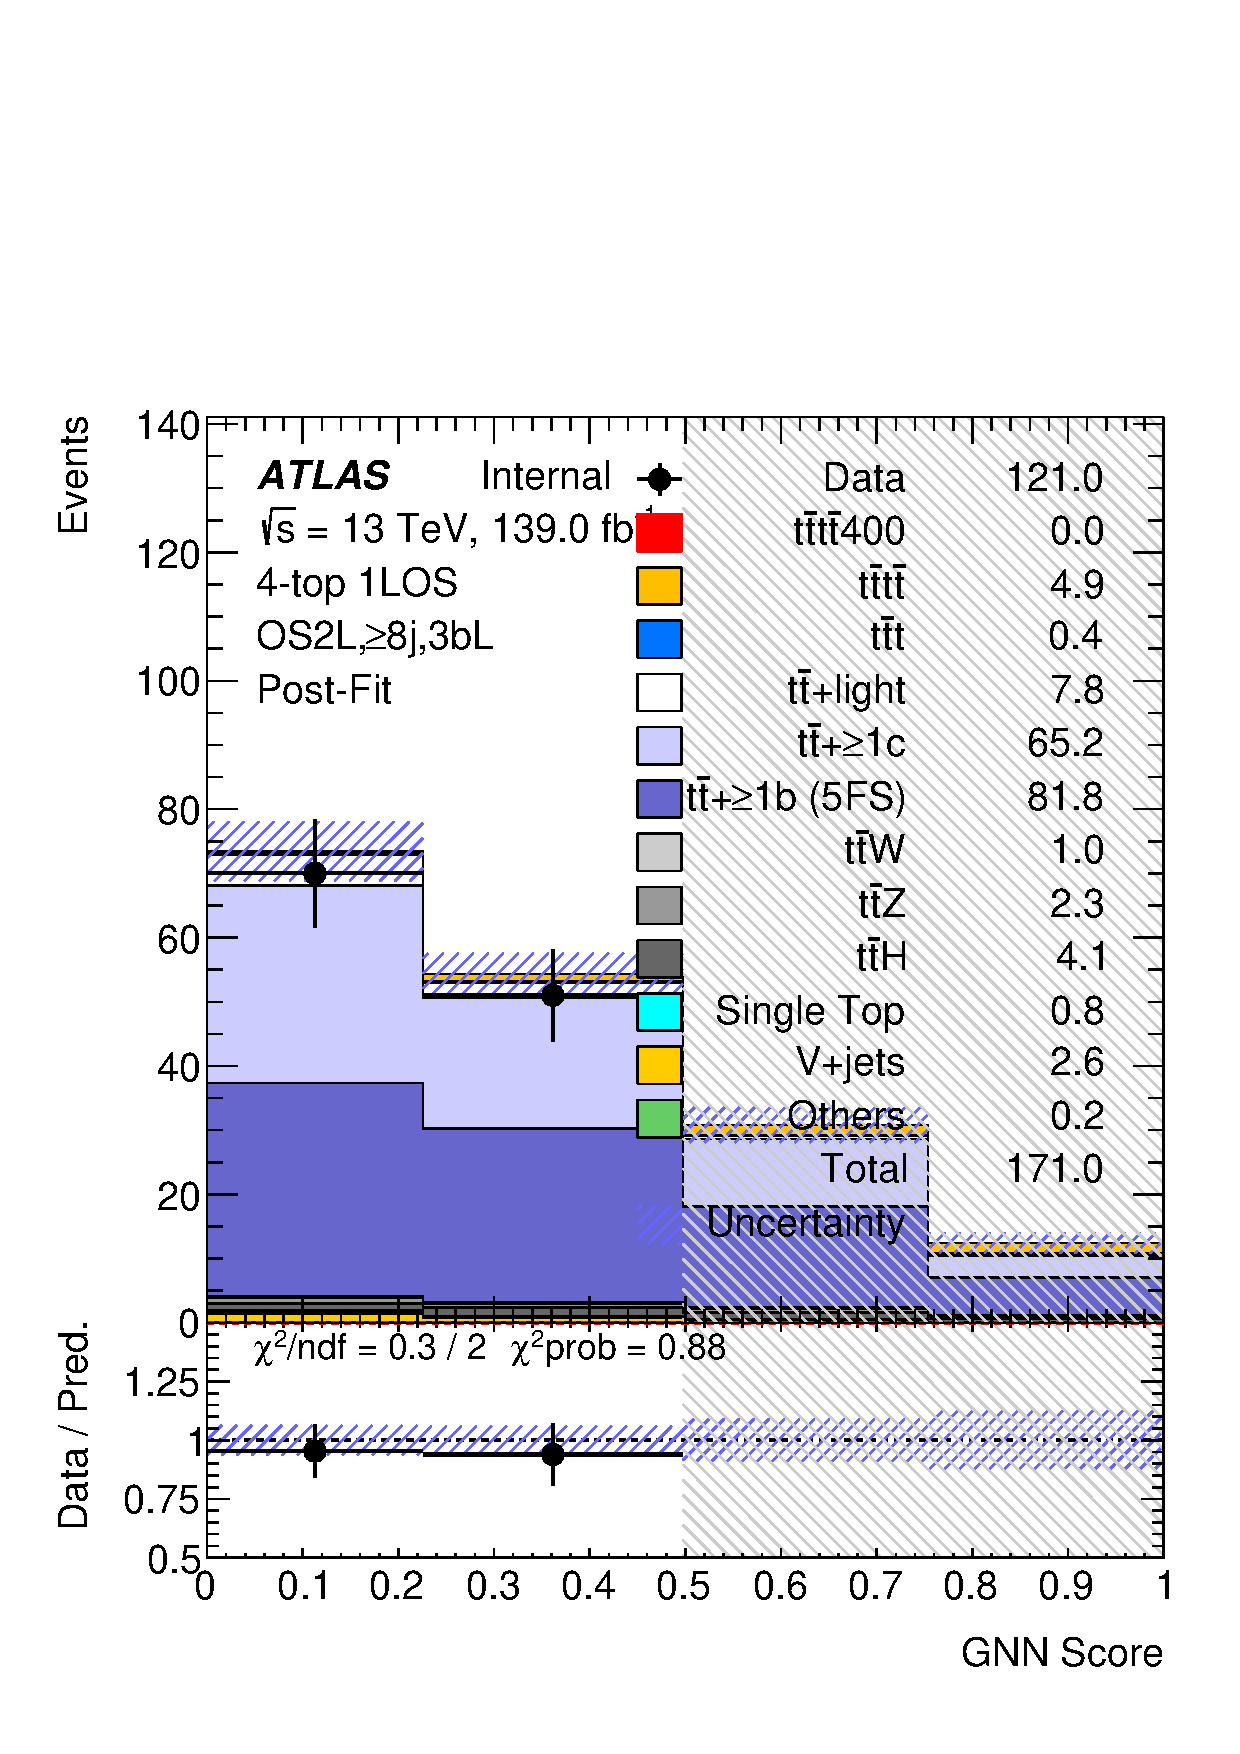
\includegraphics[width=0.31 \textwidth]{figures/fits/GNN/400/all/data/Plots/os2l_ge8j3bL_postFit.pdf} &
        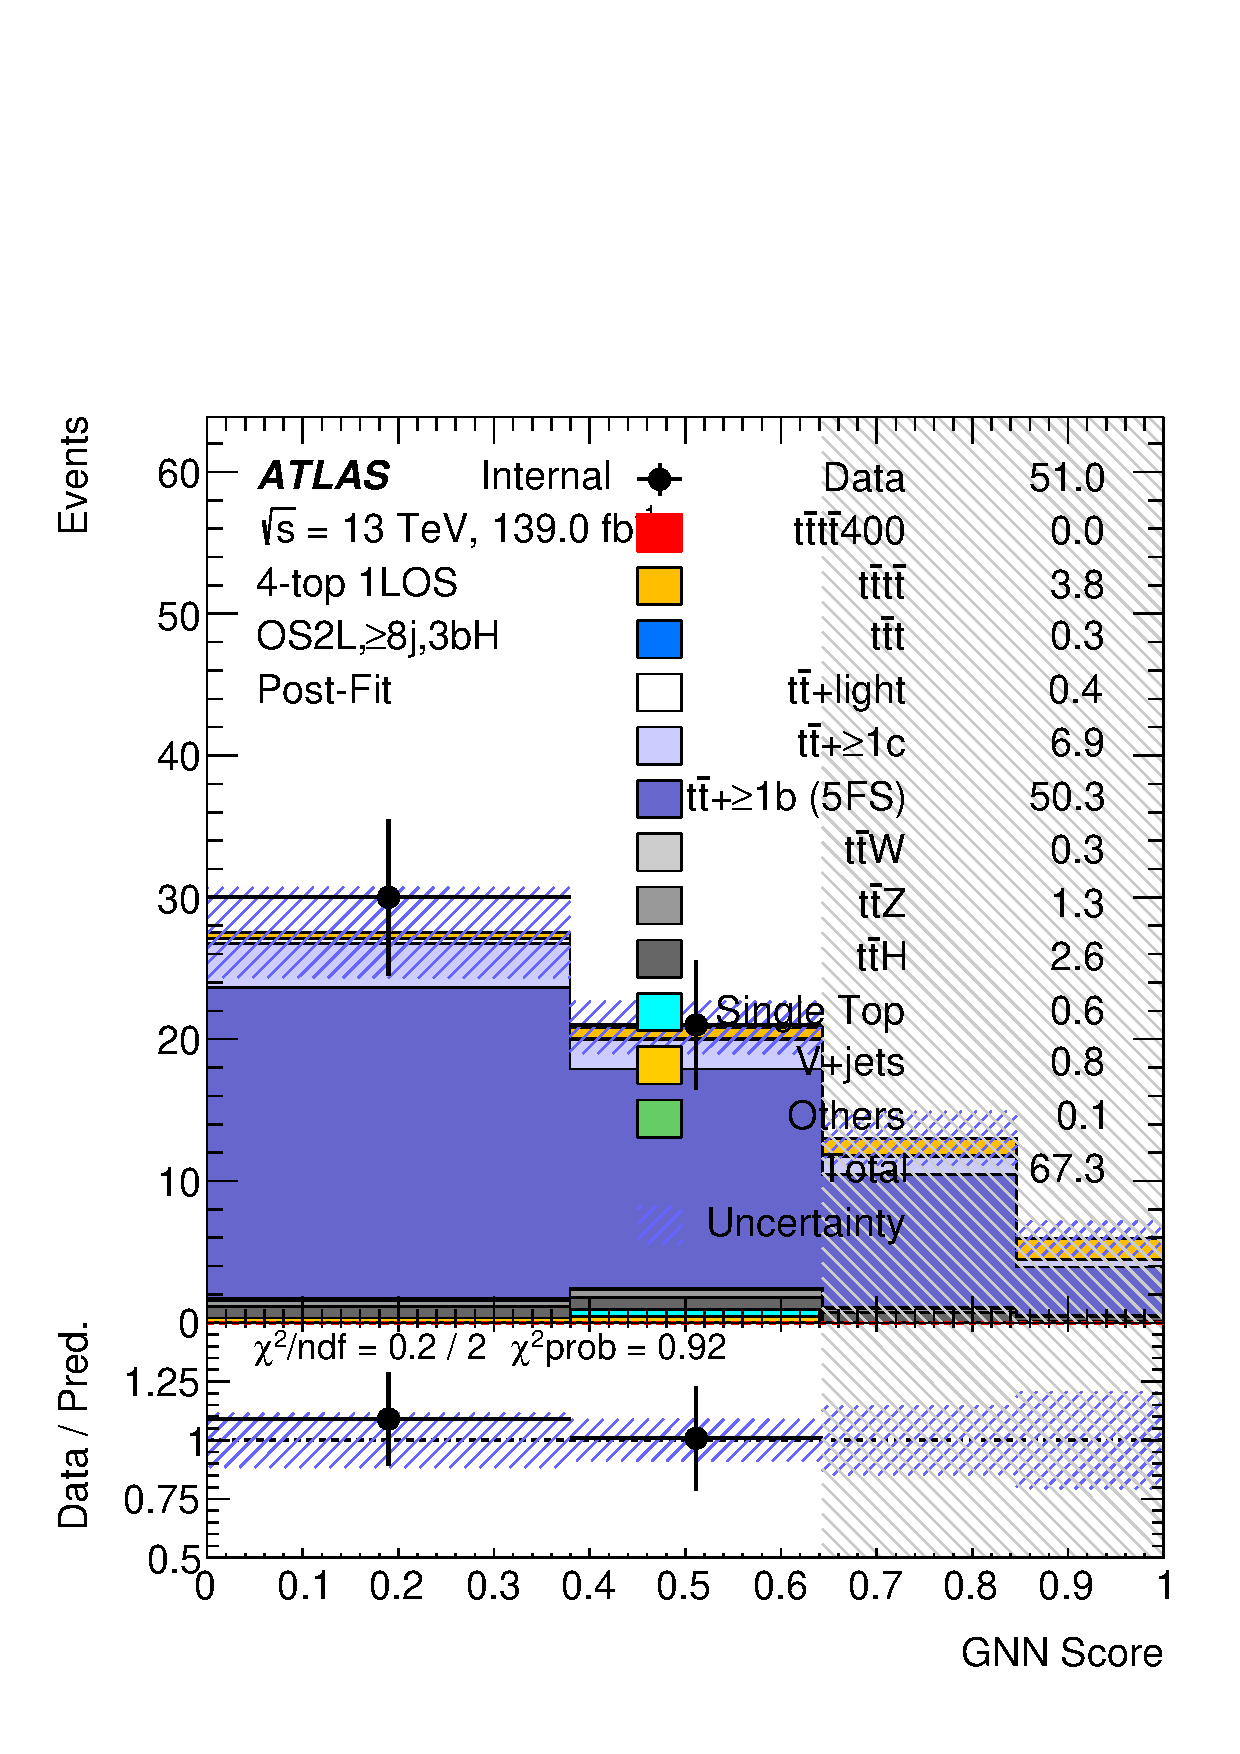
\includegraphics[width=0.31 \textwidth]{figures/fits/GNN/400/all/data/Plots/os2l_ge8j3bH_postFit.pdf} &
        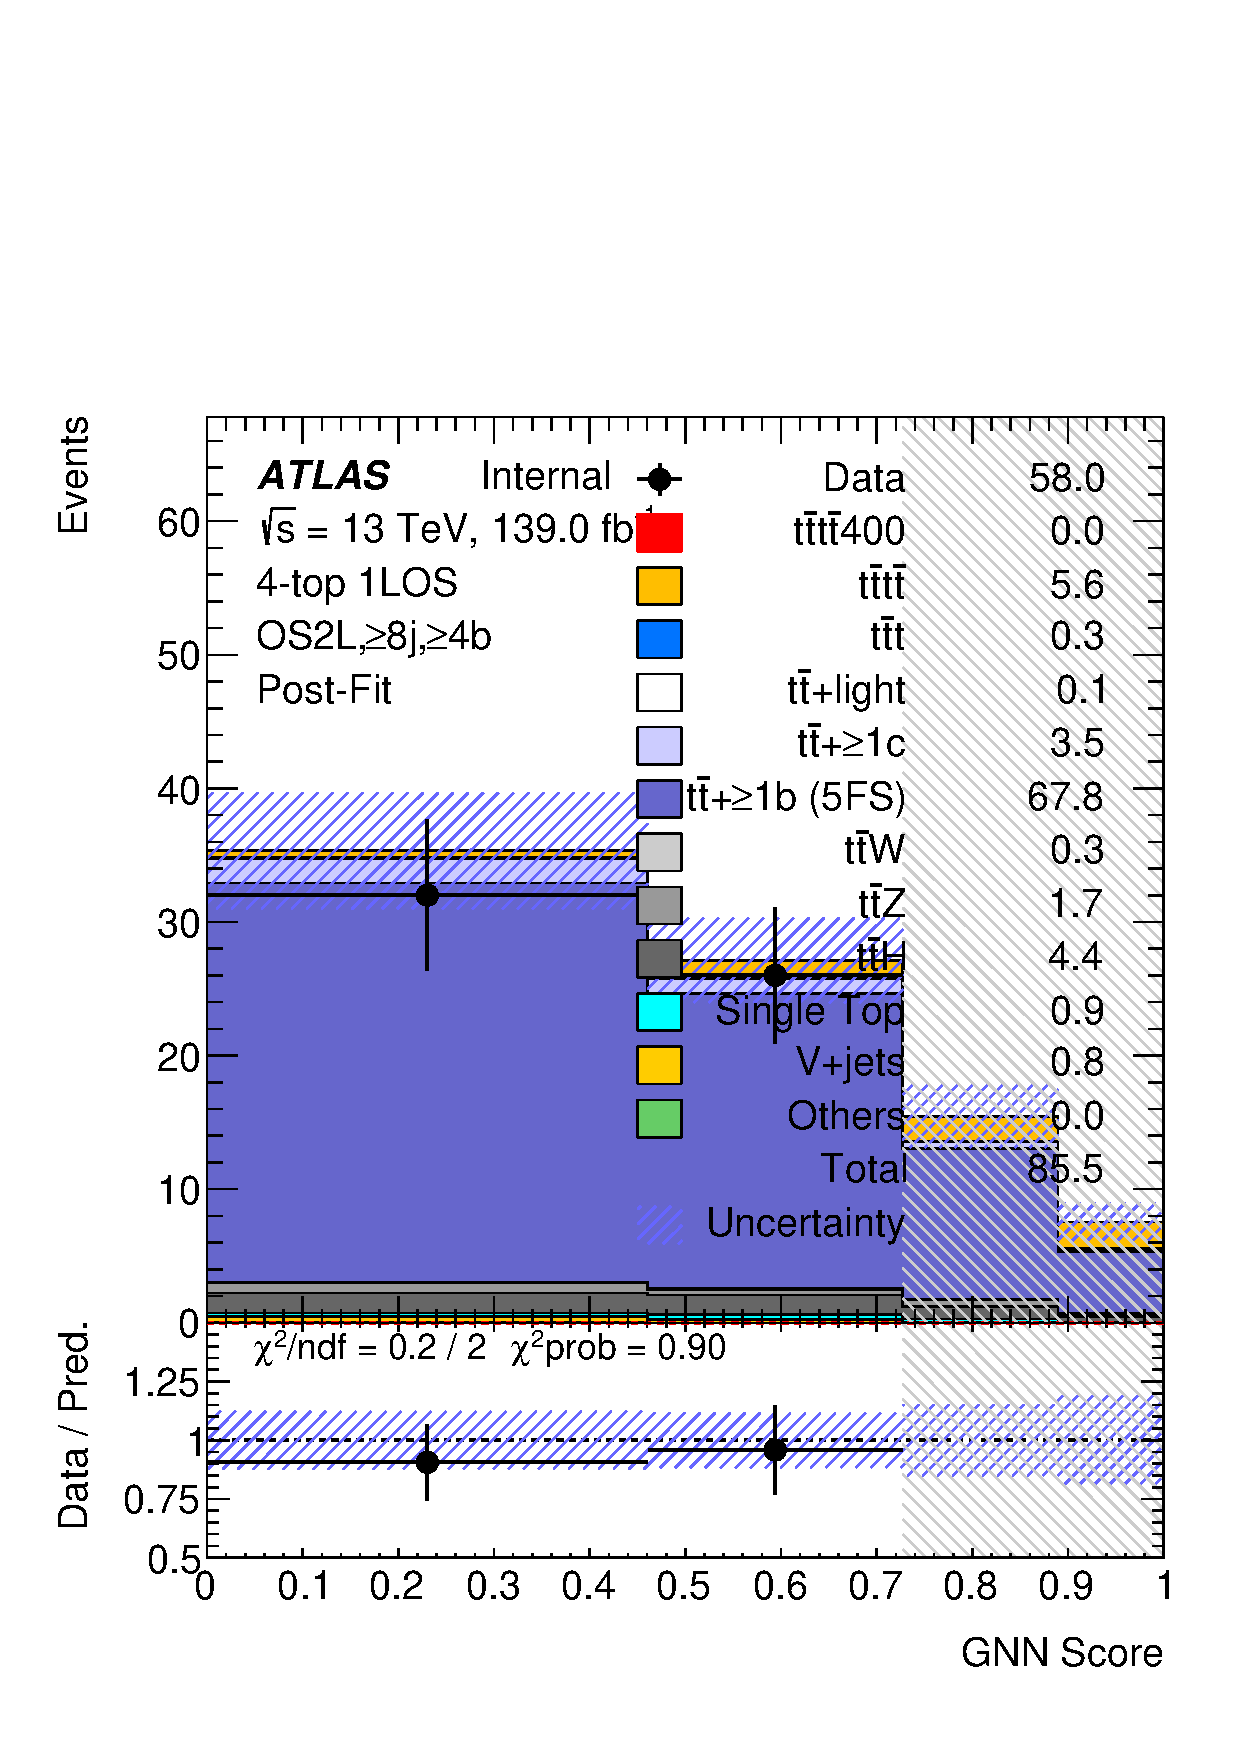
\includegraphics[width=0.31 \textwidth]{figures/fits/GNN/400/all/data/Plots/os2l_ge8jge4b_postFit.pdf} \\
        \end{tabular}
        \caption{\label{fig:Postfit_Yields_2L}Post-fit distributions for 2LOS regions associated with different signal and background samples, compared with data yields for mH = 400 GeV. The fit is done using all regions (1L+2L)}
\end{center}
\end{figure}


\begin{figure}[htbp!]
  \centering
  \begin{subfigure}[t]{0.32\textwidth}
    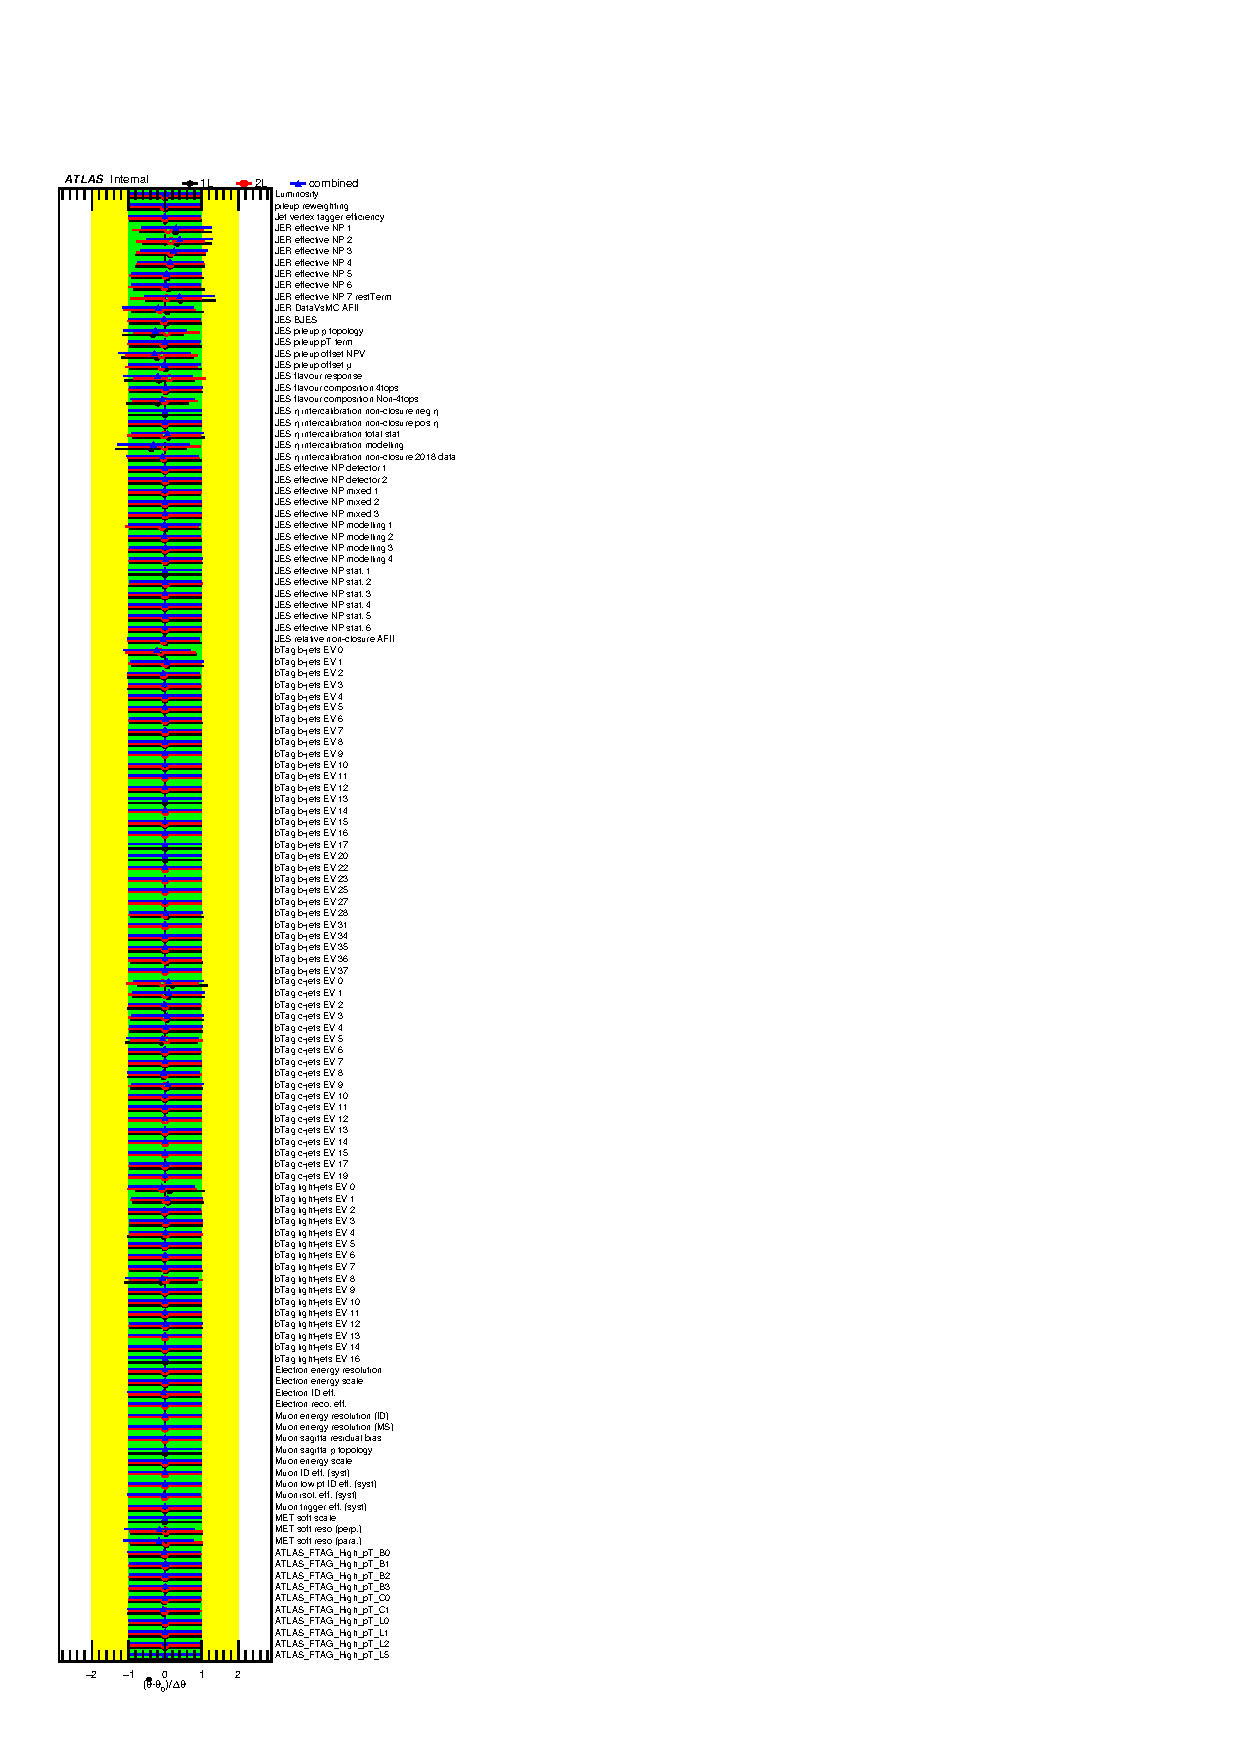
\includegraphics[width=\linewidth]{figures/fits/comparisons/selections/GNN/400/data/NuisPar_comp_Instrumental.pdf}
    \subcaption{mH=400\gev}
    \label{fig:data_NP_mH400}
  \end{subfigure}
  \begin{subfigure}[t]{0.32\textwidth}
    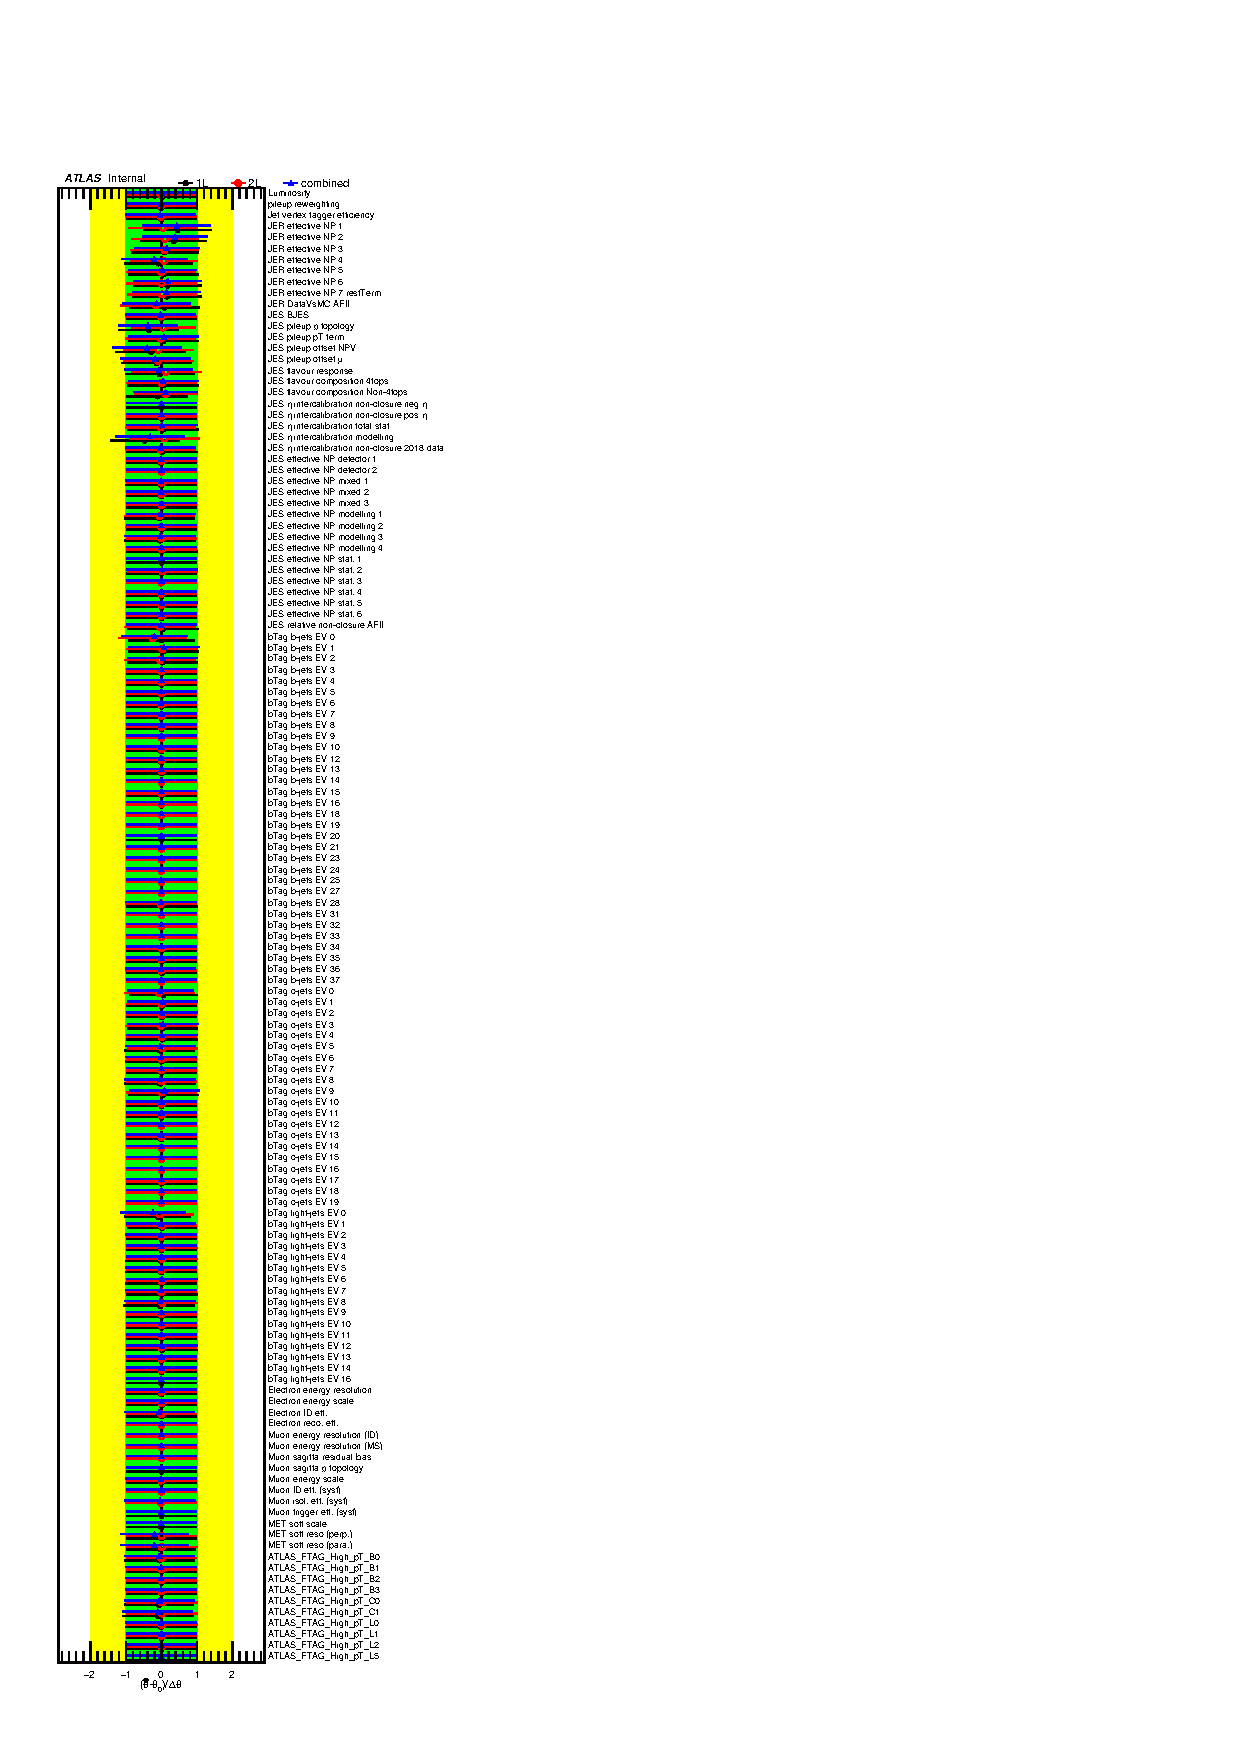
\includegraphics[width=\linewidth]{figures/fits/comparisons/selections/GNN/700/data/NuisPar_comp_Instrumental.pdf}
    \subcaption{mH=700\gev}
    \label{fig:data_NP_mH400}
  \end{subfigure}
  \begin{subfigure}[t]{0.32\textwidth}
    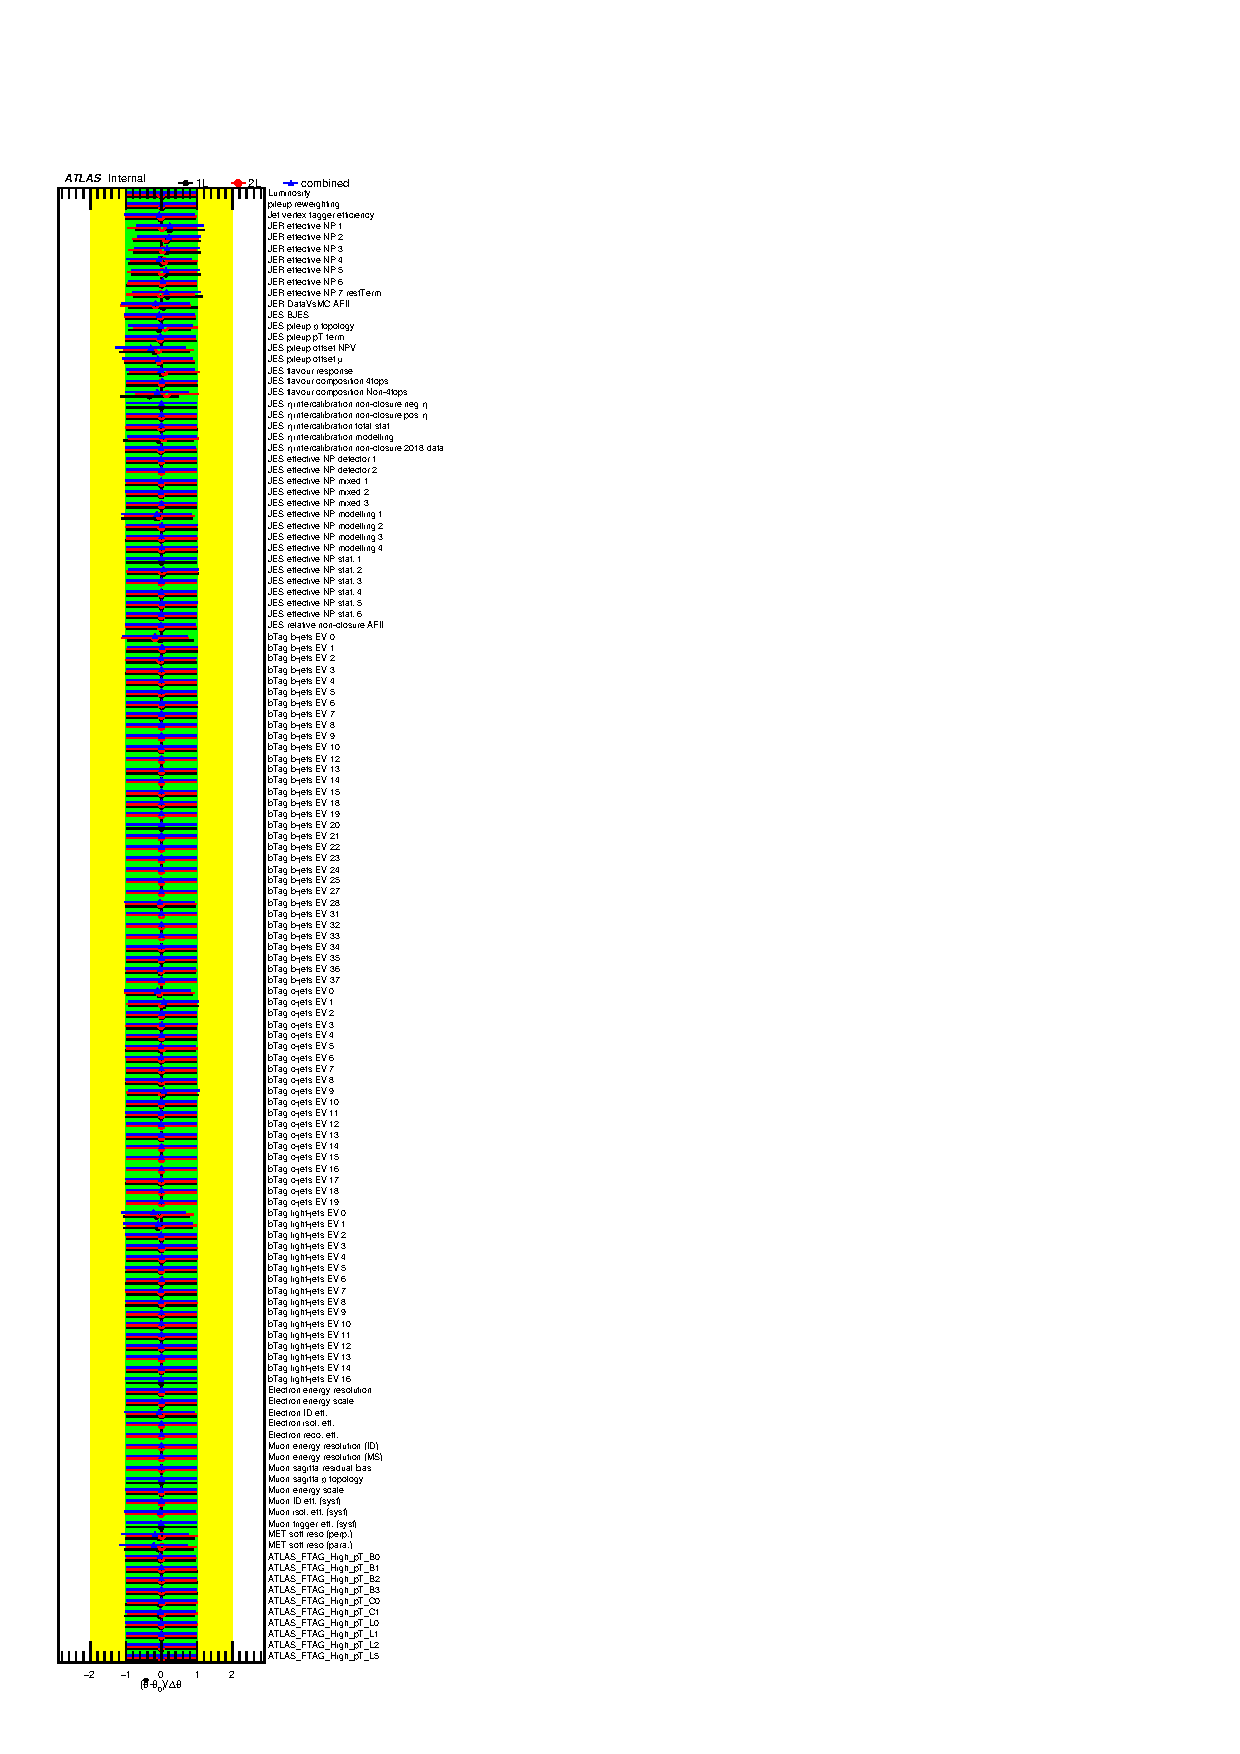
\includegraphics[width=\linewidth]{figures/fits/comparisons/selections/GNN/1000/data/NuisPar_comp_Instrumental.pdf}
    \subcaption{mH=1000\gev}
    \label{fig:data_NP_mH400}
  \end{subfigure}
  \caption{\label{fig:data_NP_instrumental}Fitted pulls and constraints for the nuisance parameters corresponding to the instrumental systematic uncertainties for the blinded Data fit for three mass points. Comparison is done for three fits: using only 1L regions, using only 2LOS regions and using all regions.}
\end{figure}


\begin{figure}[htbp!]
  \centering
  \begin{subfigure}[t]{0.32\textwidth}
    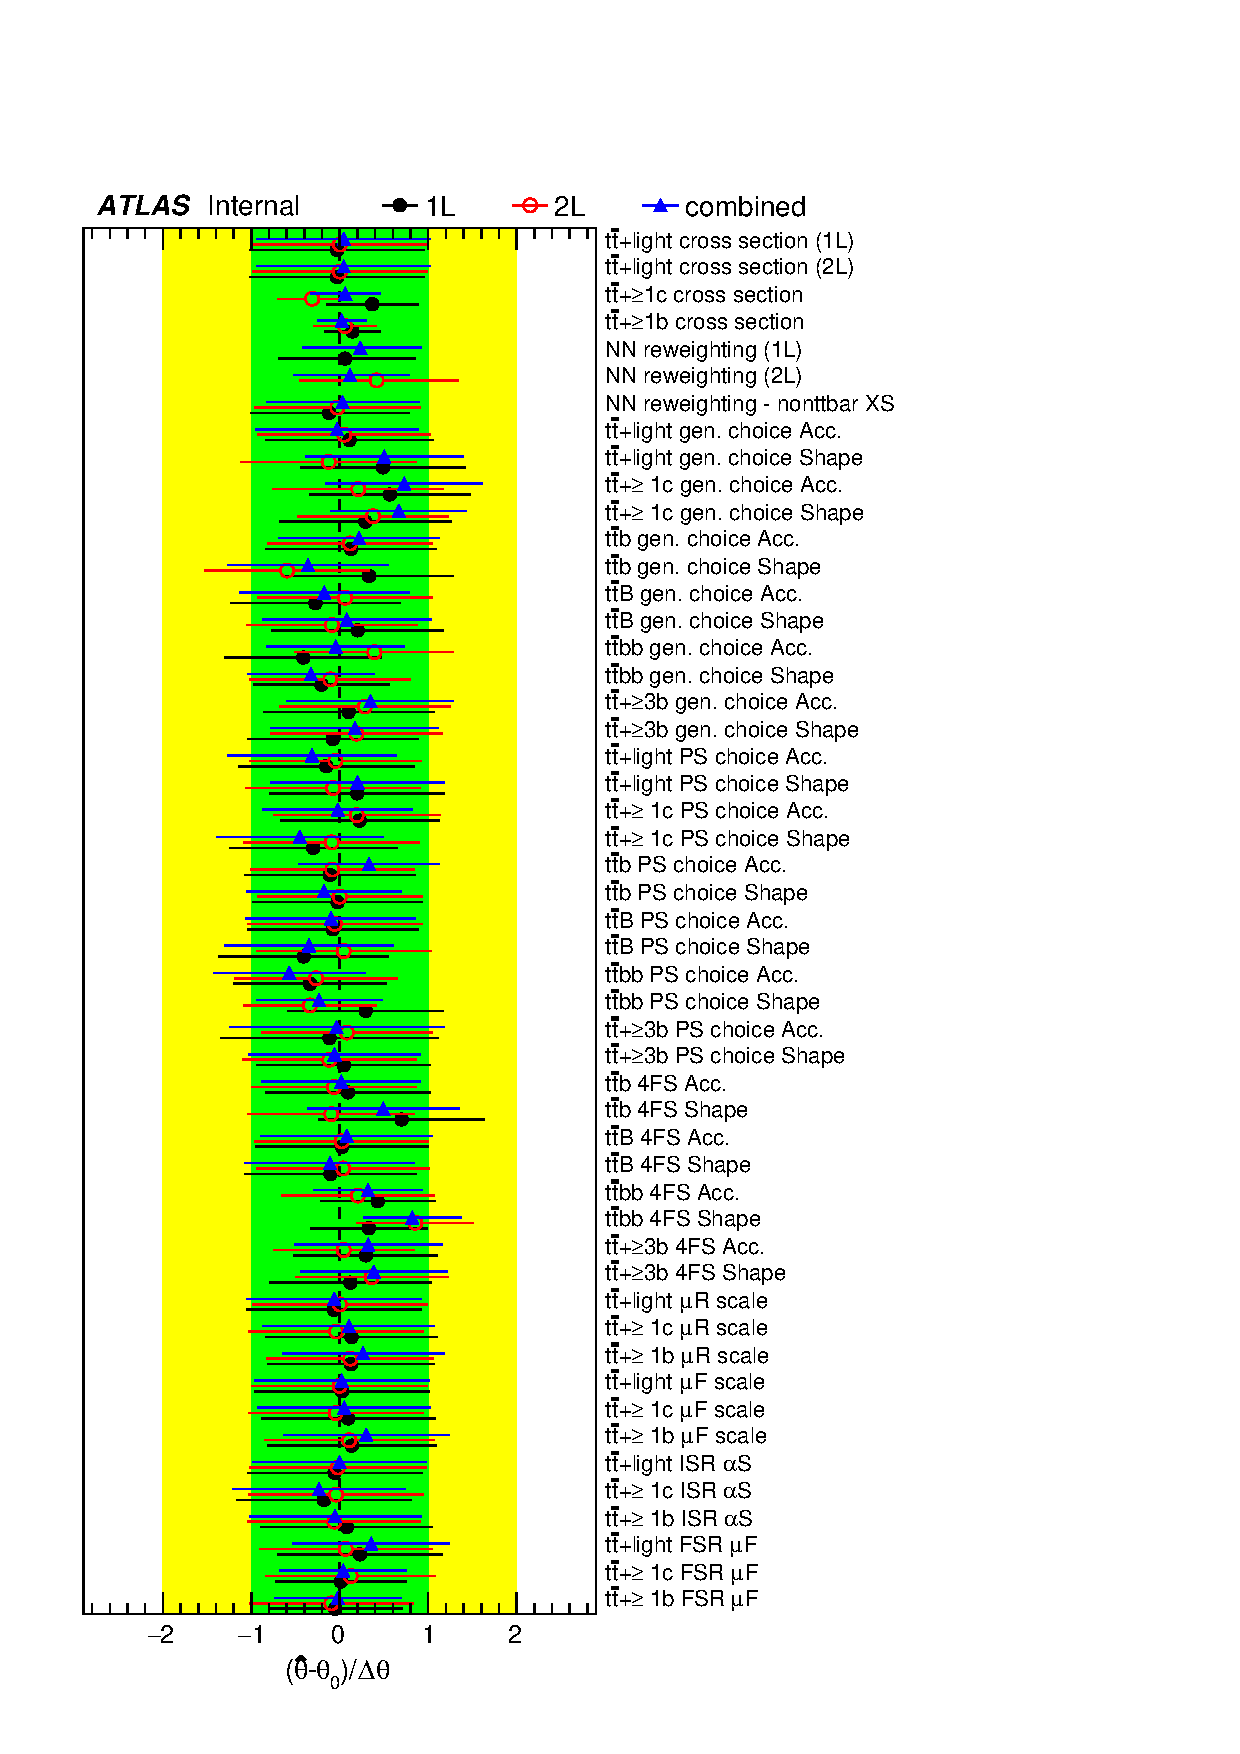
\includegraphics[width=\linewidth]{figures/fits/comparisons/selections/GNN/400/data/NuisPar_comp_ttbar.pdf}
    \subcaption{mH=400\gev}
    \label{fig:data_NP_mH400}
  \end{subfigure}
  \begin{subfigure}[t]{0.32\textwidth}
    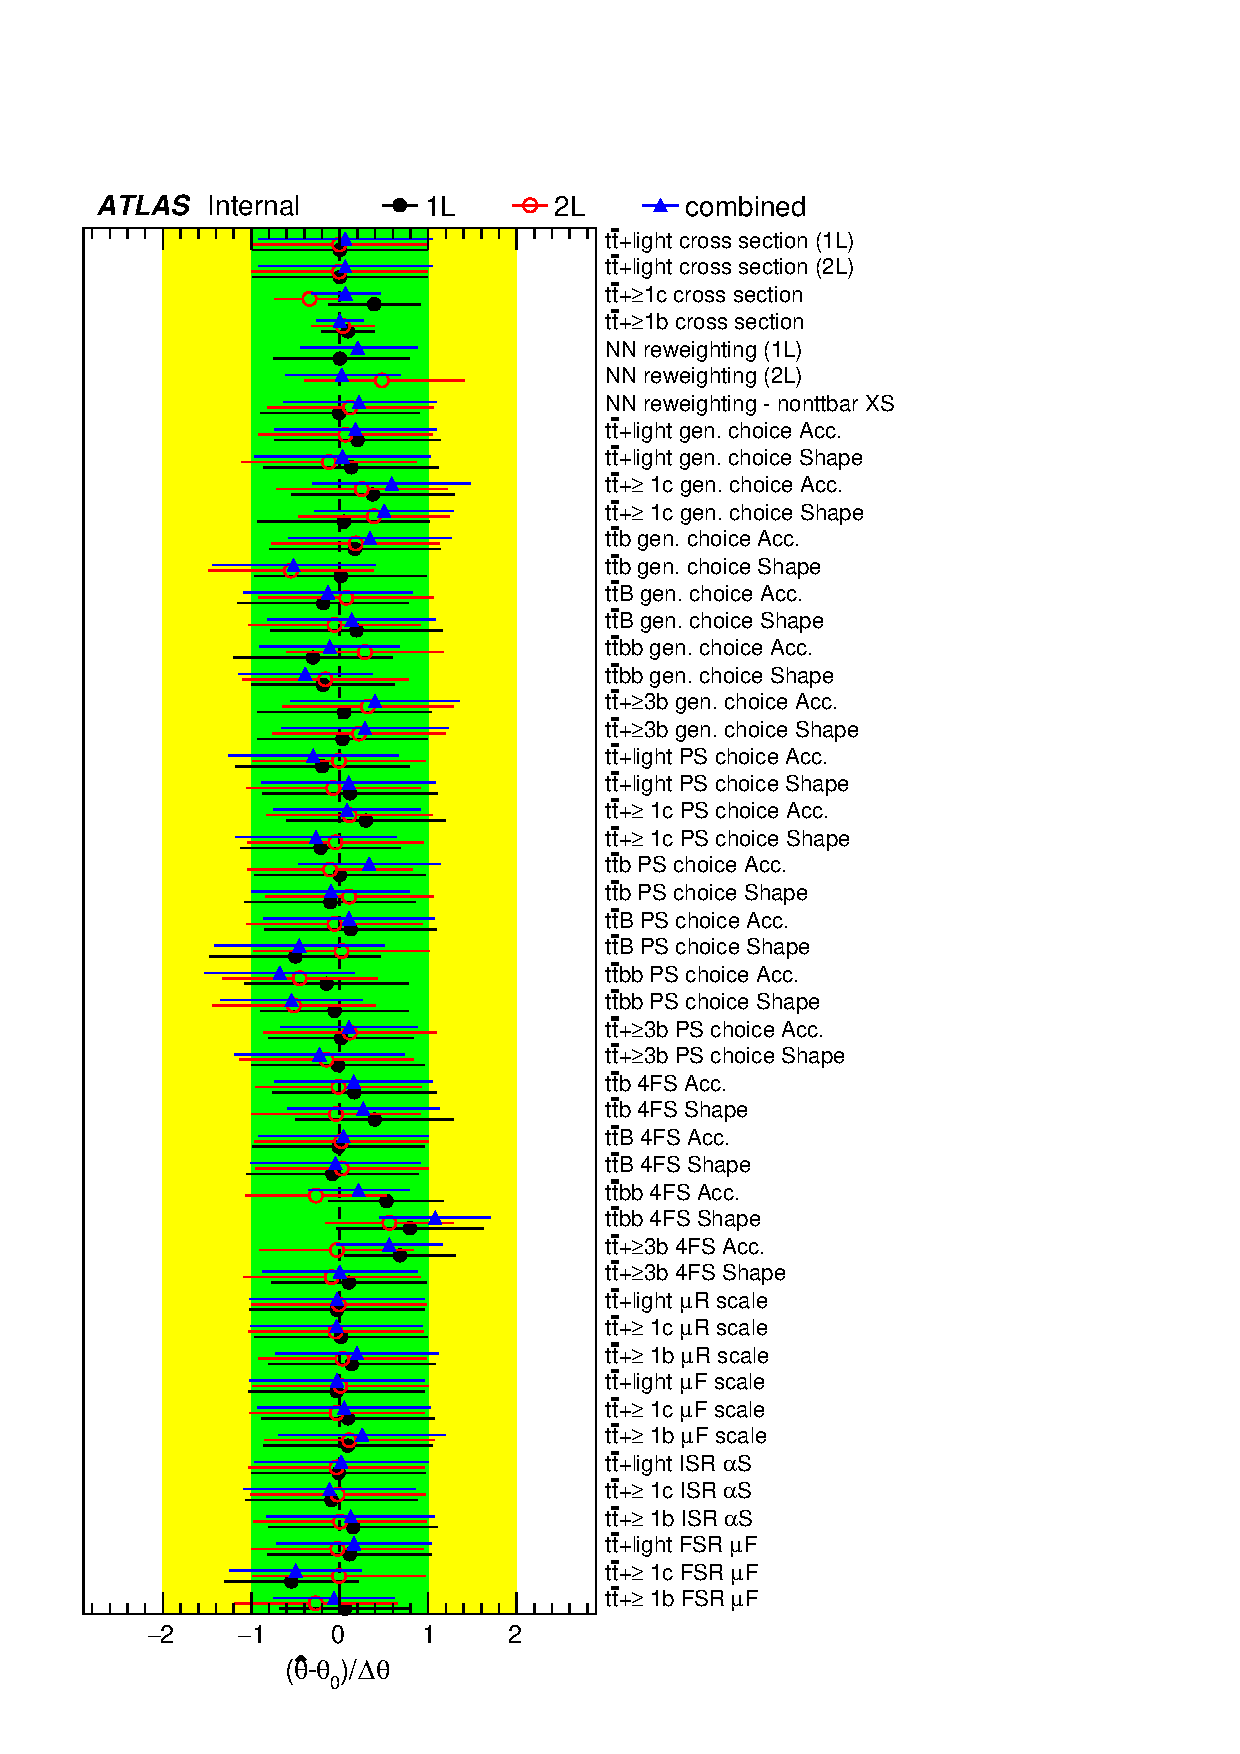
\includegraphics[width=\linewidth]{figures/fits/comparisons/selections/GNN/700/data/NuisPar_comp_ttbar.pdf}
    \subcaption{mH=700\gev}
    \label{fig:data_NP_mH400}
  \end{subfigure}
  \begin{subfigure}[t]{0.32\textwidth}
    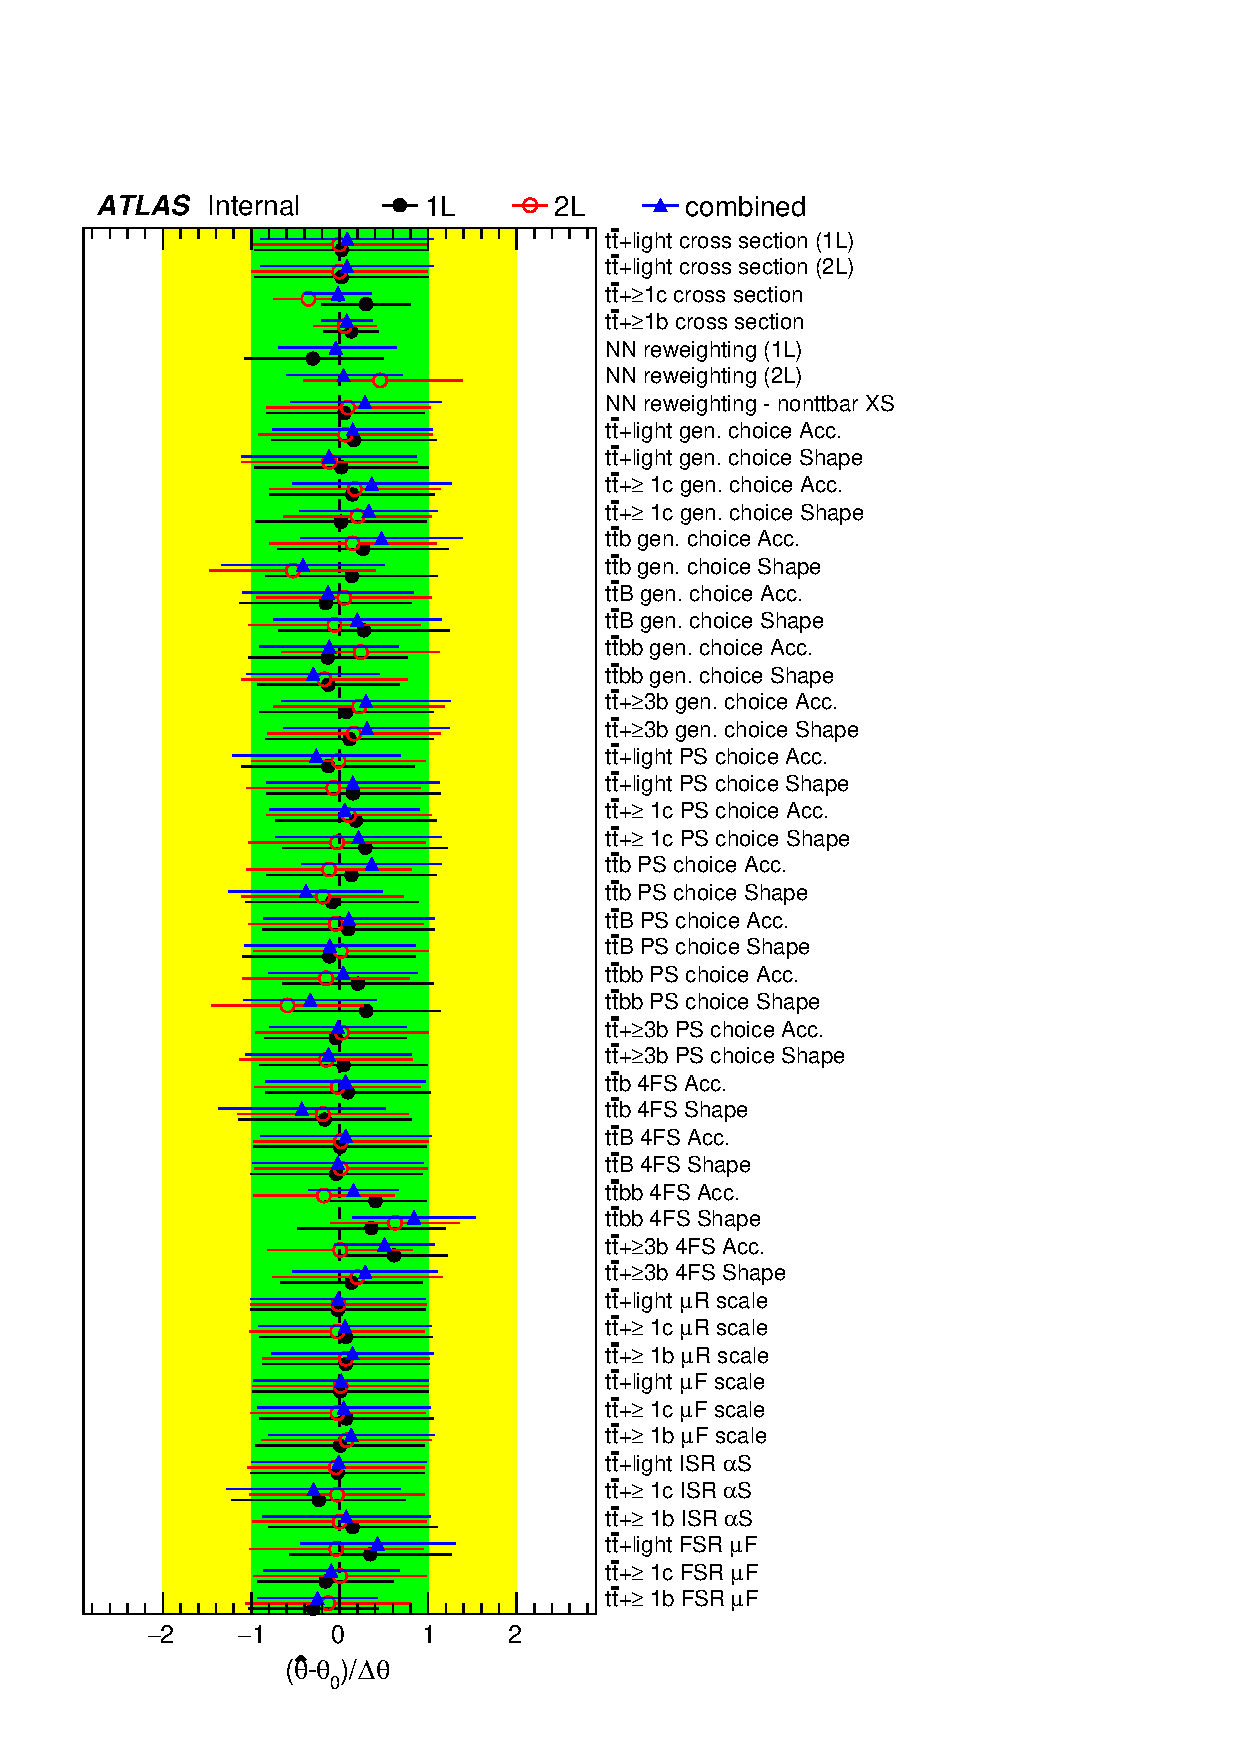
\includegraphics[width=\linewidth]{figures/fits/comparisons/selections/GNN/1000/data/NuisPar_comp_ttbar.pdf}
    \subcaption{mH=1000\gev}
    \label{fig:data_NP_mH400}
  \end{subfigure}
  \caption{\label{fig:data_NP_ttbar}Fitted pulls and constraints for the nuisance parameters corresponding to the \ttbar systematic uncertainties for the blinded Data fit for three mass points. Comparison is done for three fits: using only 1L regions, using only 2LOS regions and using all regions.}
\end{figure}


\begin{figure}[htbp!]
  \centering
  \begin{subfigure}[t]{0.32\textwidth}
    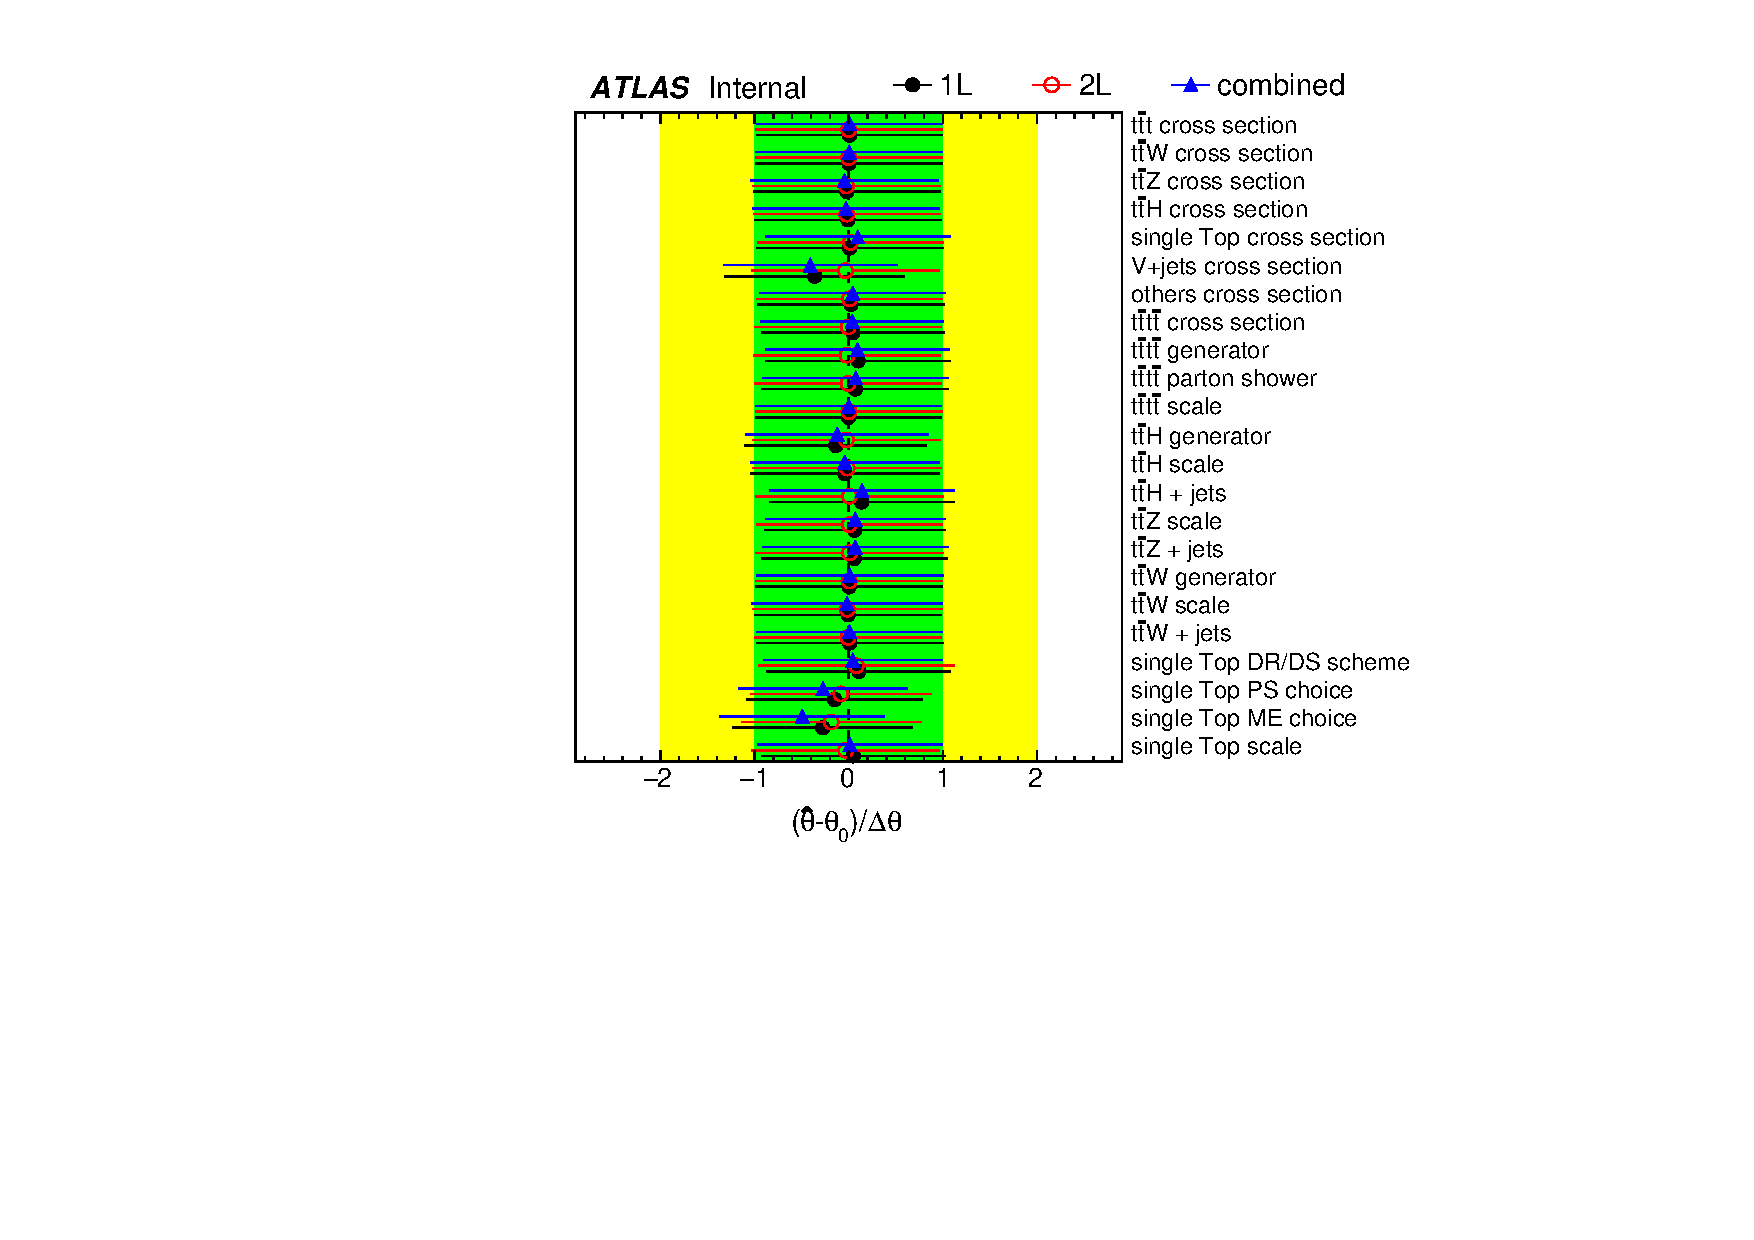
\includegraphics[width=\linewidth]{figures/fits/comparisons/selections/GNN/400/data/NuisPar_comp_Other.pdf}
    \subcaption{mH=400\gev}
    \label{fig:data_NP_mH400}
  \end{subfigure}
  \begin{subfigure}[t]{0.32\textwidth}
    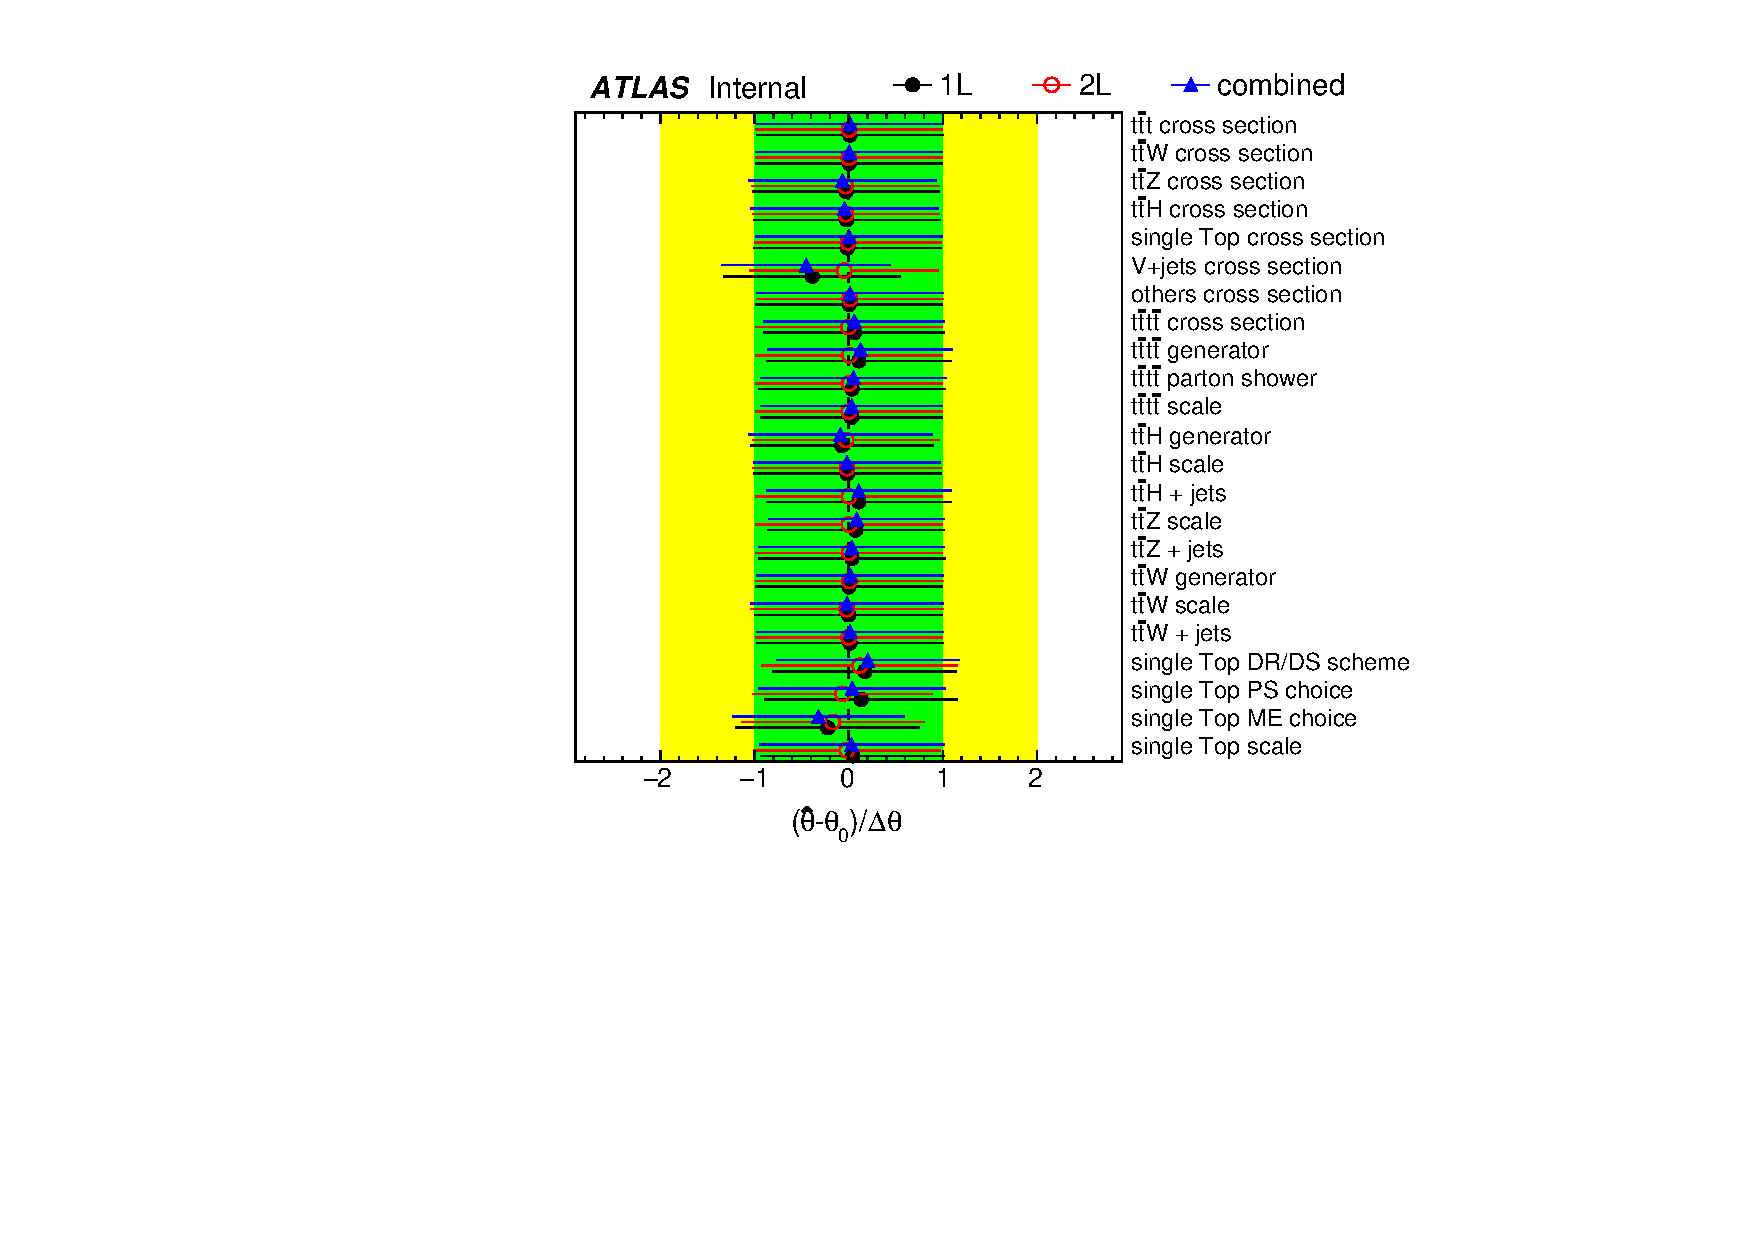
\includegraphics[width=\linewidth]{figures/fits/comparisons/selections/GNN/700/data/NuisPar_comp_Other.pdf}
    \subcaption{mH=700\gev}
    \label{fig:data_NP_mH400}
  \end{subfigure}
  \begin{subfigure}[t]{0.32\textwidth}
    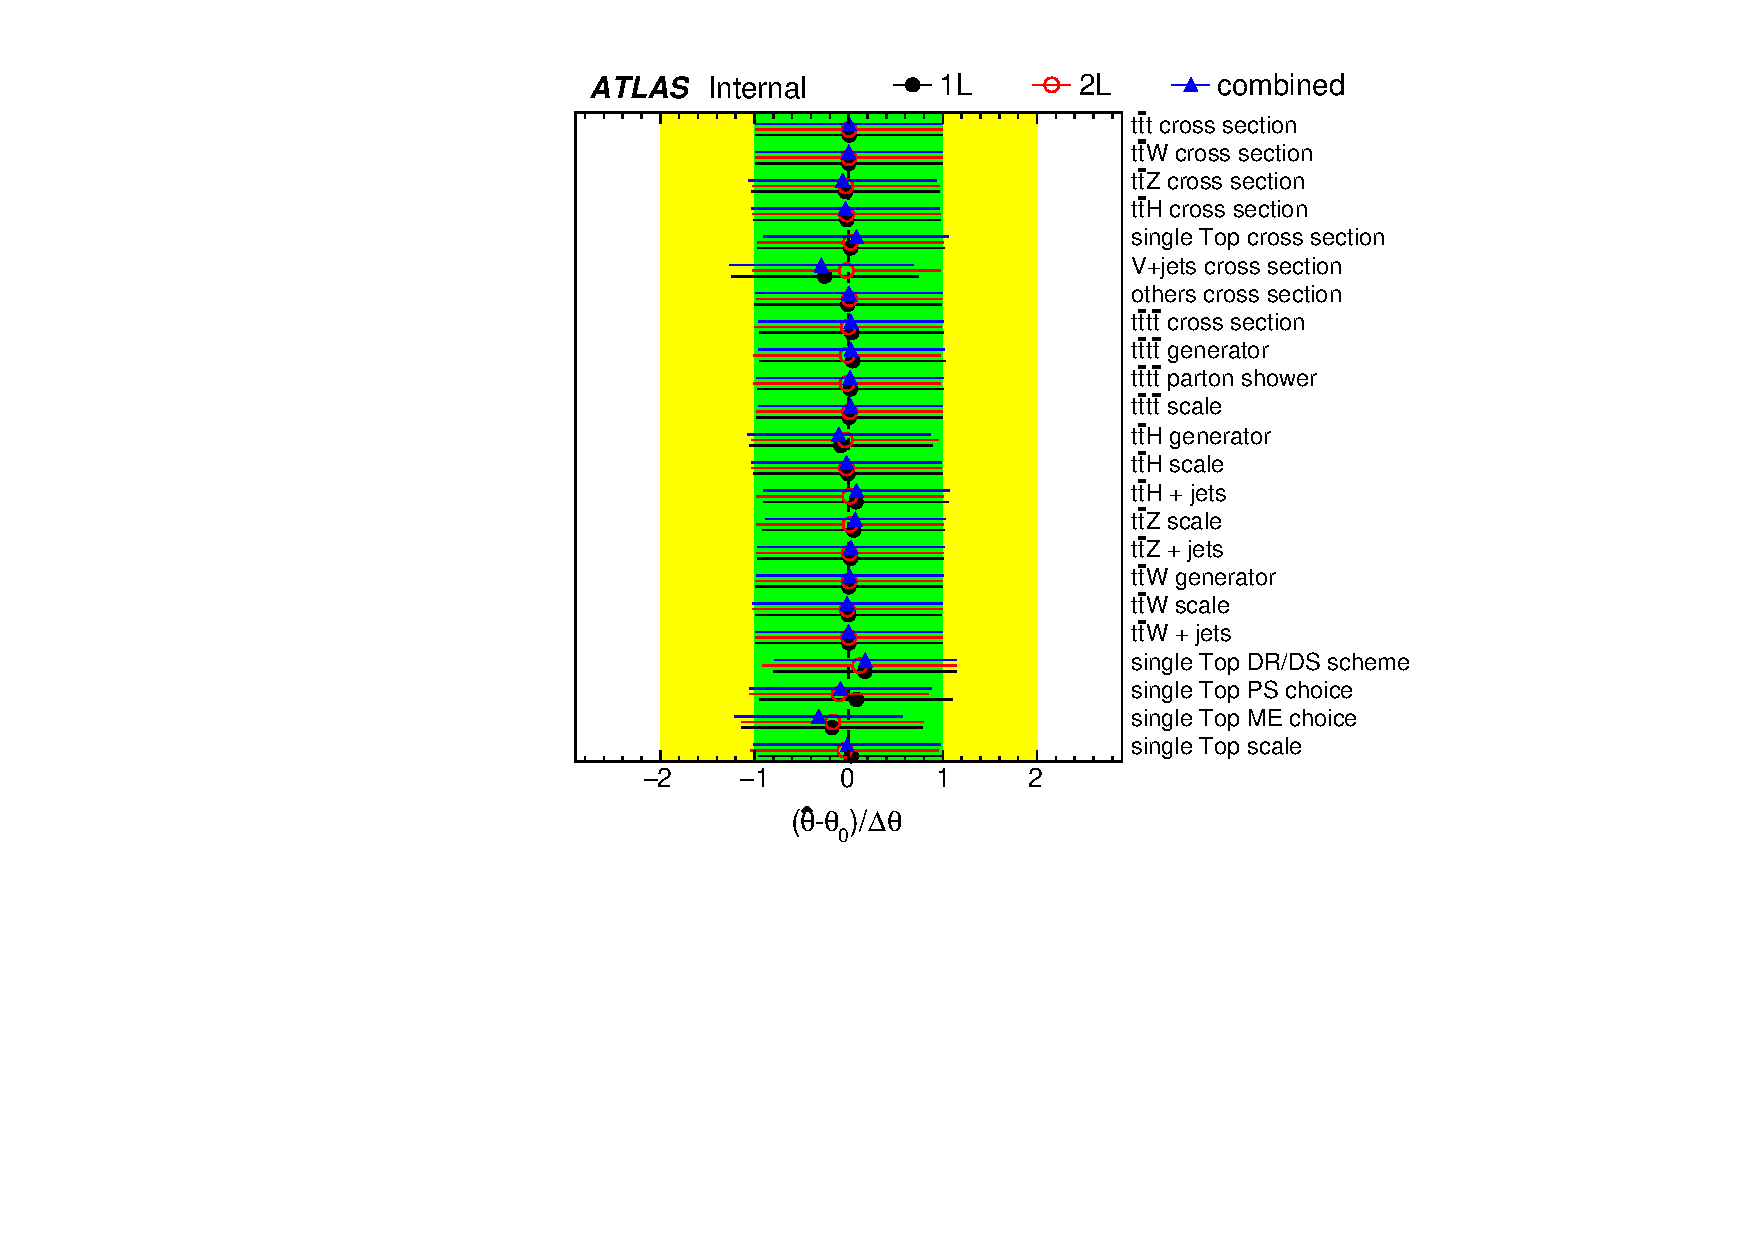
\includegraphics[width=\linewidth]{figures/fits/comparisons/selections/GNN/1000/data/NuisPar_comp_Other.pdf}
    \subcaption{mH=1000\gev}
    \label{fig:data_NP_mH400}
  \end{subfigure}
  \caption{\label{fig:data_NP_other}Fitted pulls and constraints for the  nuisance parameters corresponding to the non-\ttbar-background systematic uncertainties for the blinded Data fit for three mass points. Comparison is done for three fits: using only 1L regions, using only 2LOS regions and using all regions.}
\end{figure}



\begin{figure}[htbp!]
  \centering
  \begin{subfigure}[t]{0.32\textwidth}
    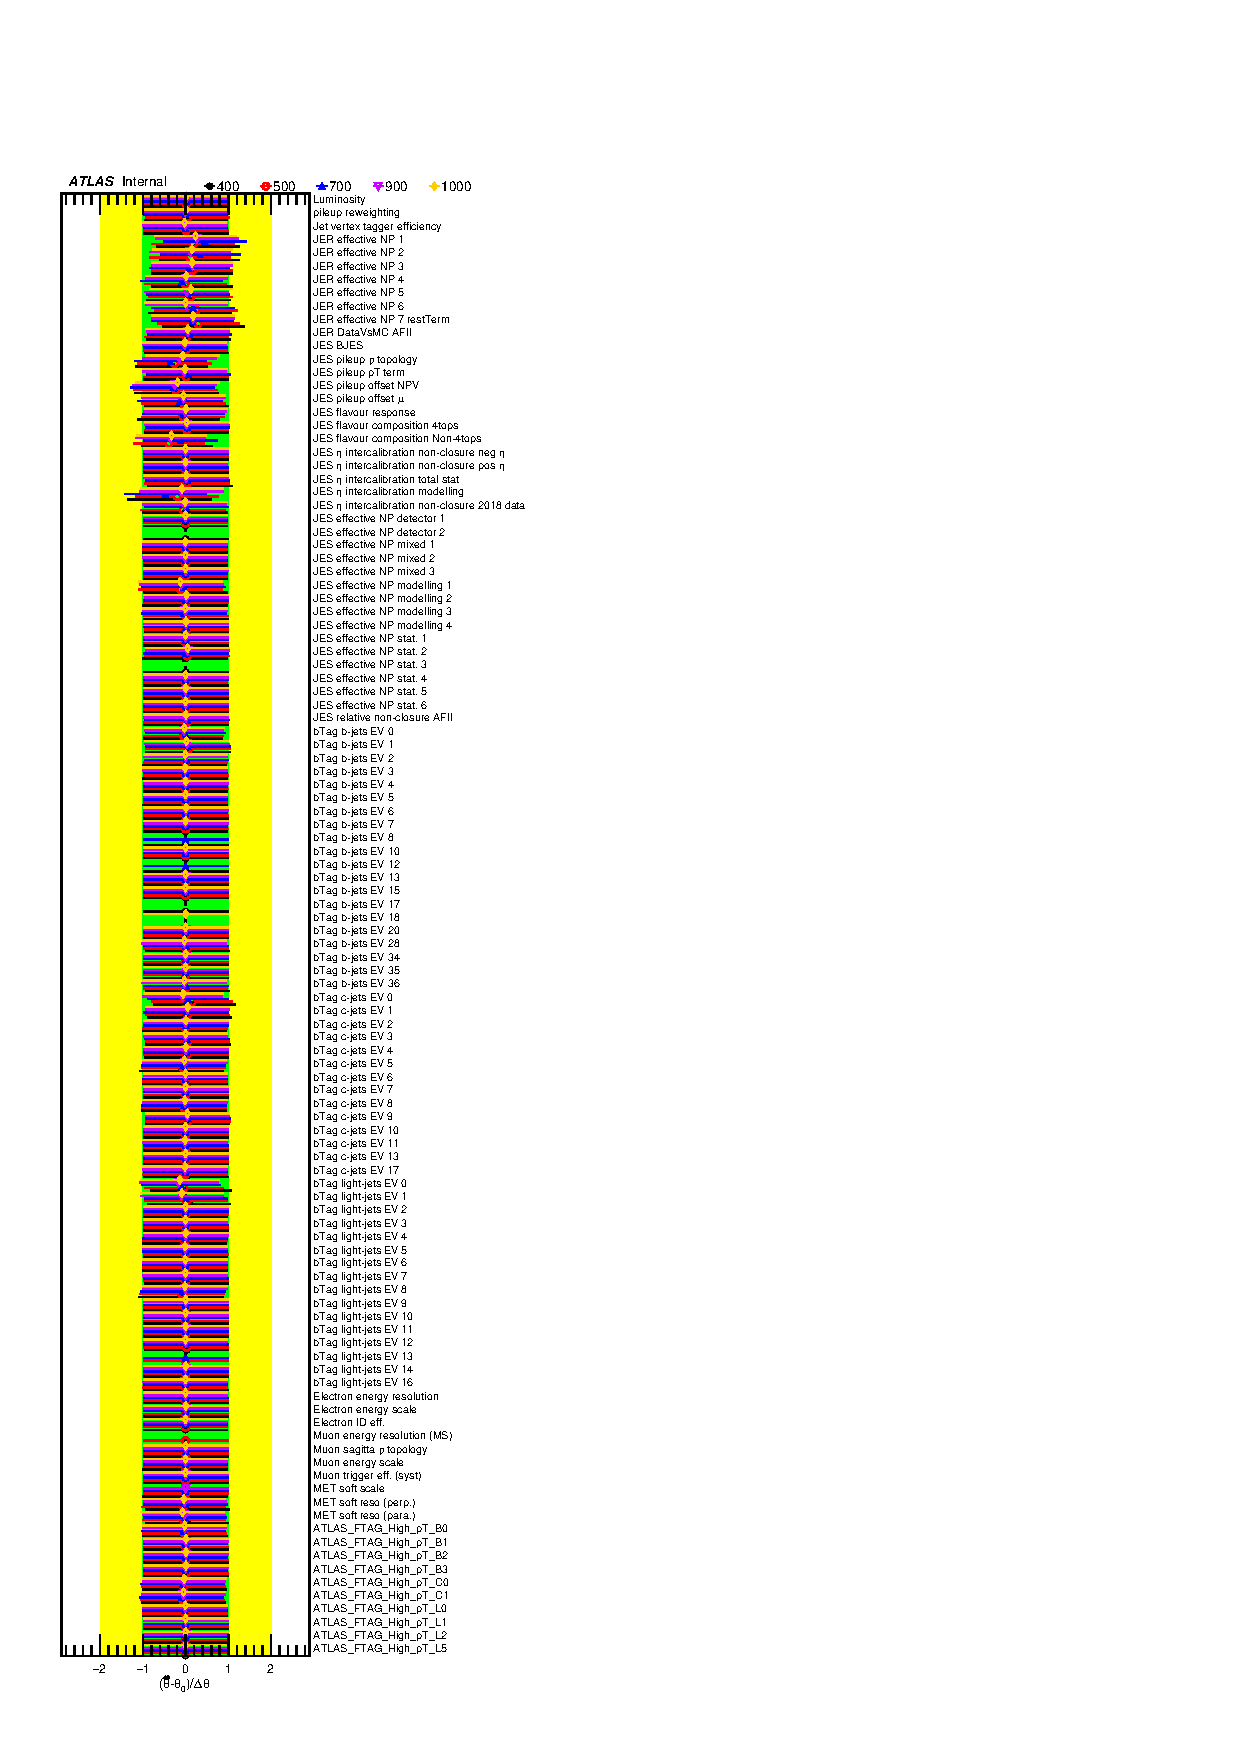
\includegraphics[width=\linewidth]{figures/fits/comparisons/massPoints/GNN/1L/data/NuisPar_comp_Instrumental.pdf}
    \subcaption{1L}
    \label{fig:data_NP_1L_instrumental}
  \end{subfigure}
  \begin{subfigure}[t]{0.32\textwidth}
    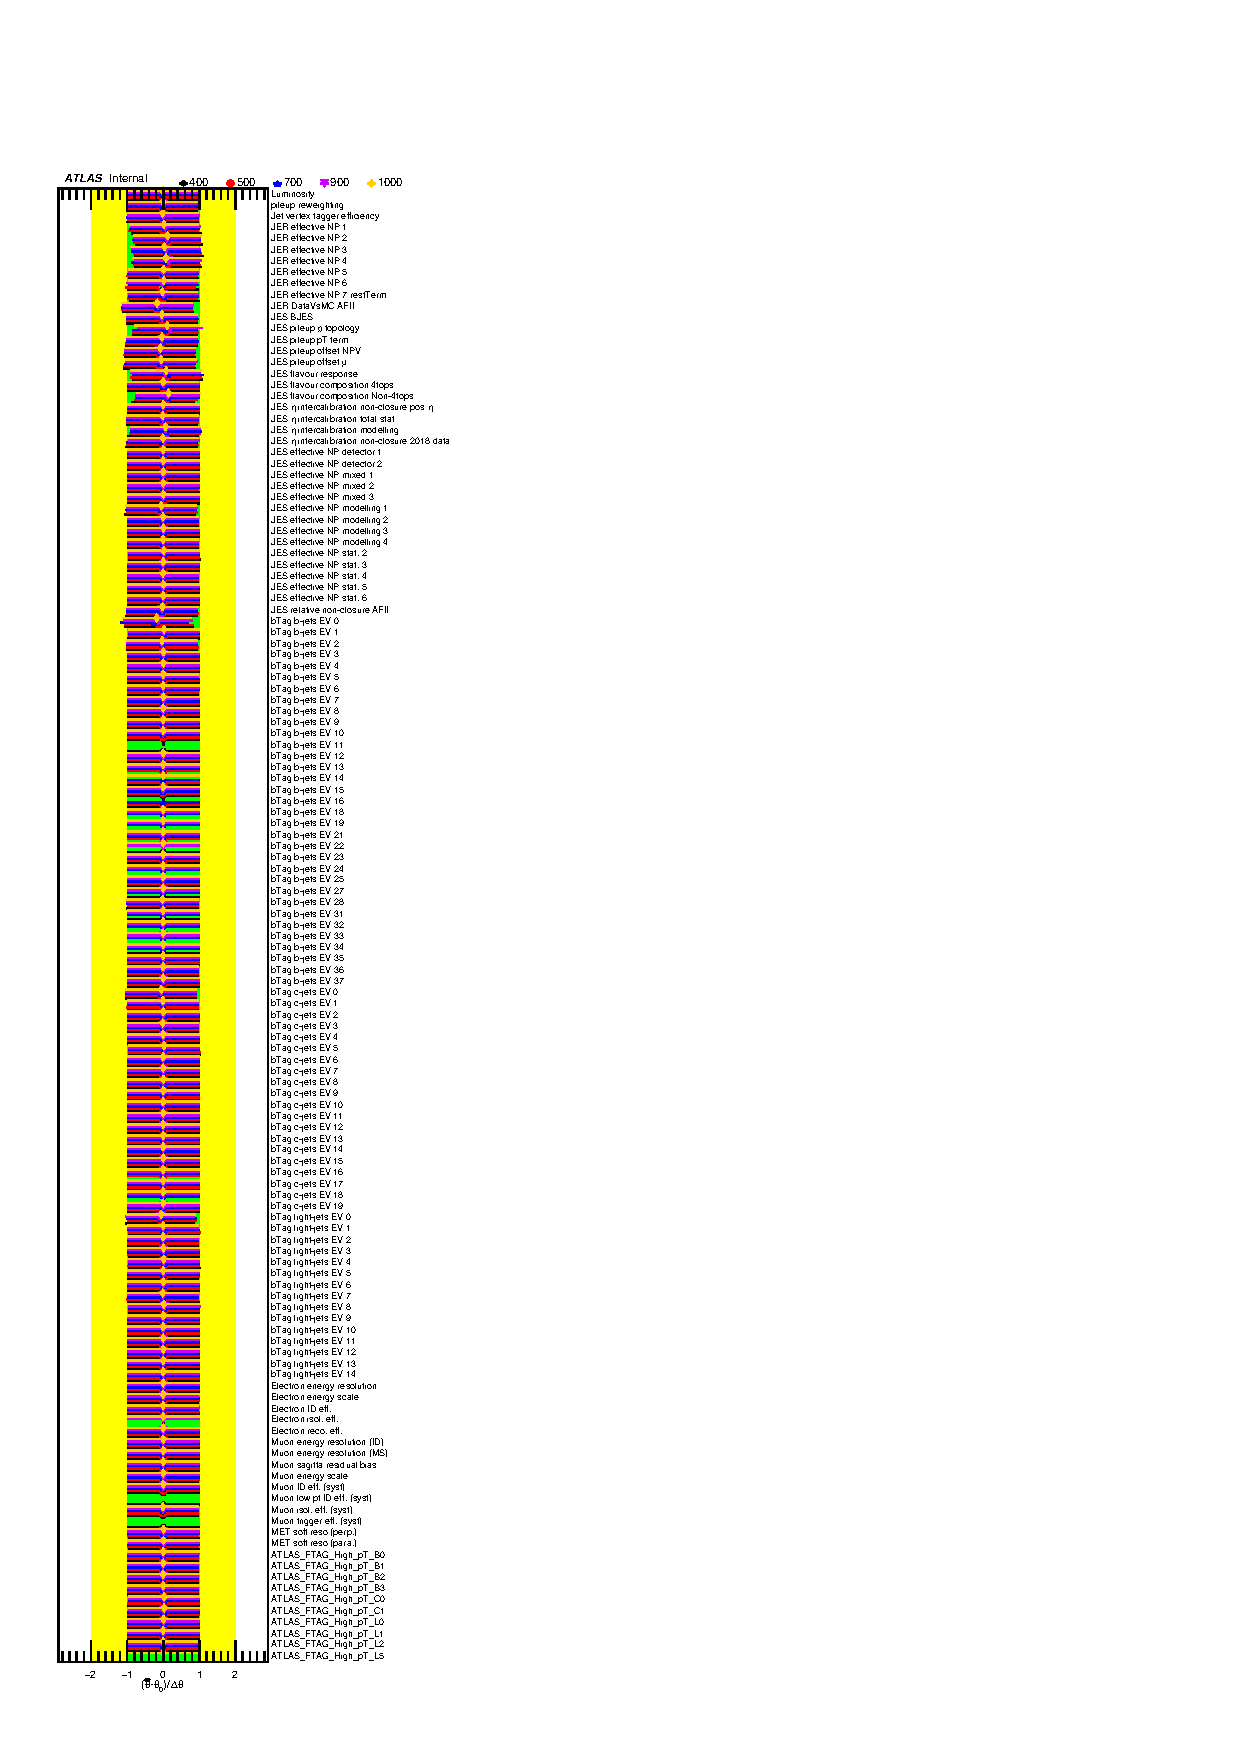
\includegraphics[width=\linewidth]{figures/fits/comparisons/massPoints/GNN/2L/data/NuisPar_comp_Instrumental.pdf}
    \subcaption{2L}
    \label{fig:data_NP_2L_instrumental}
  \end{subfigure}
  \begin{subfigure}[t]{0.32\textwidth}
    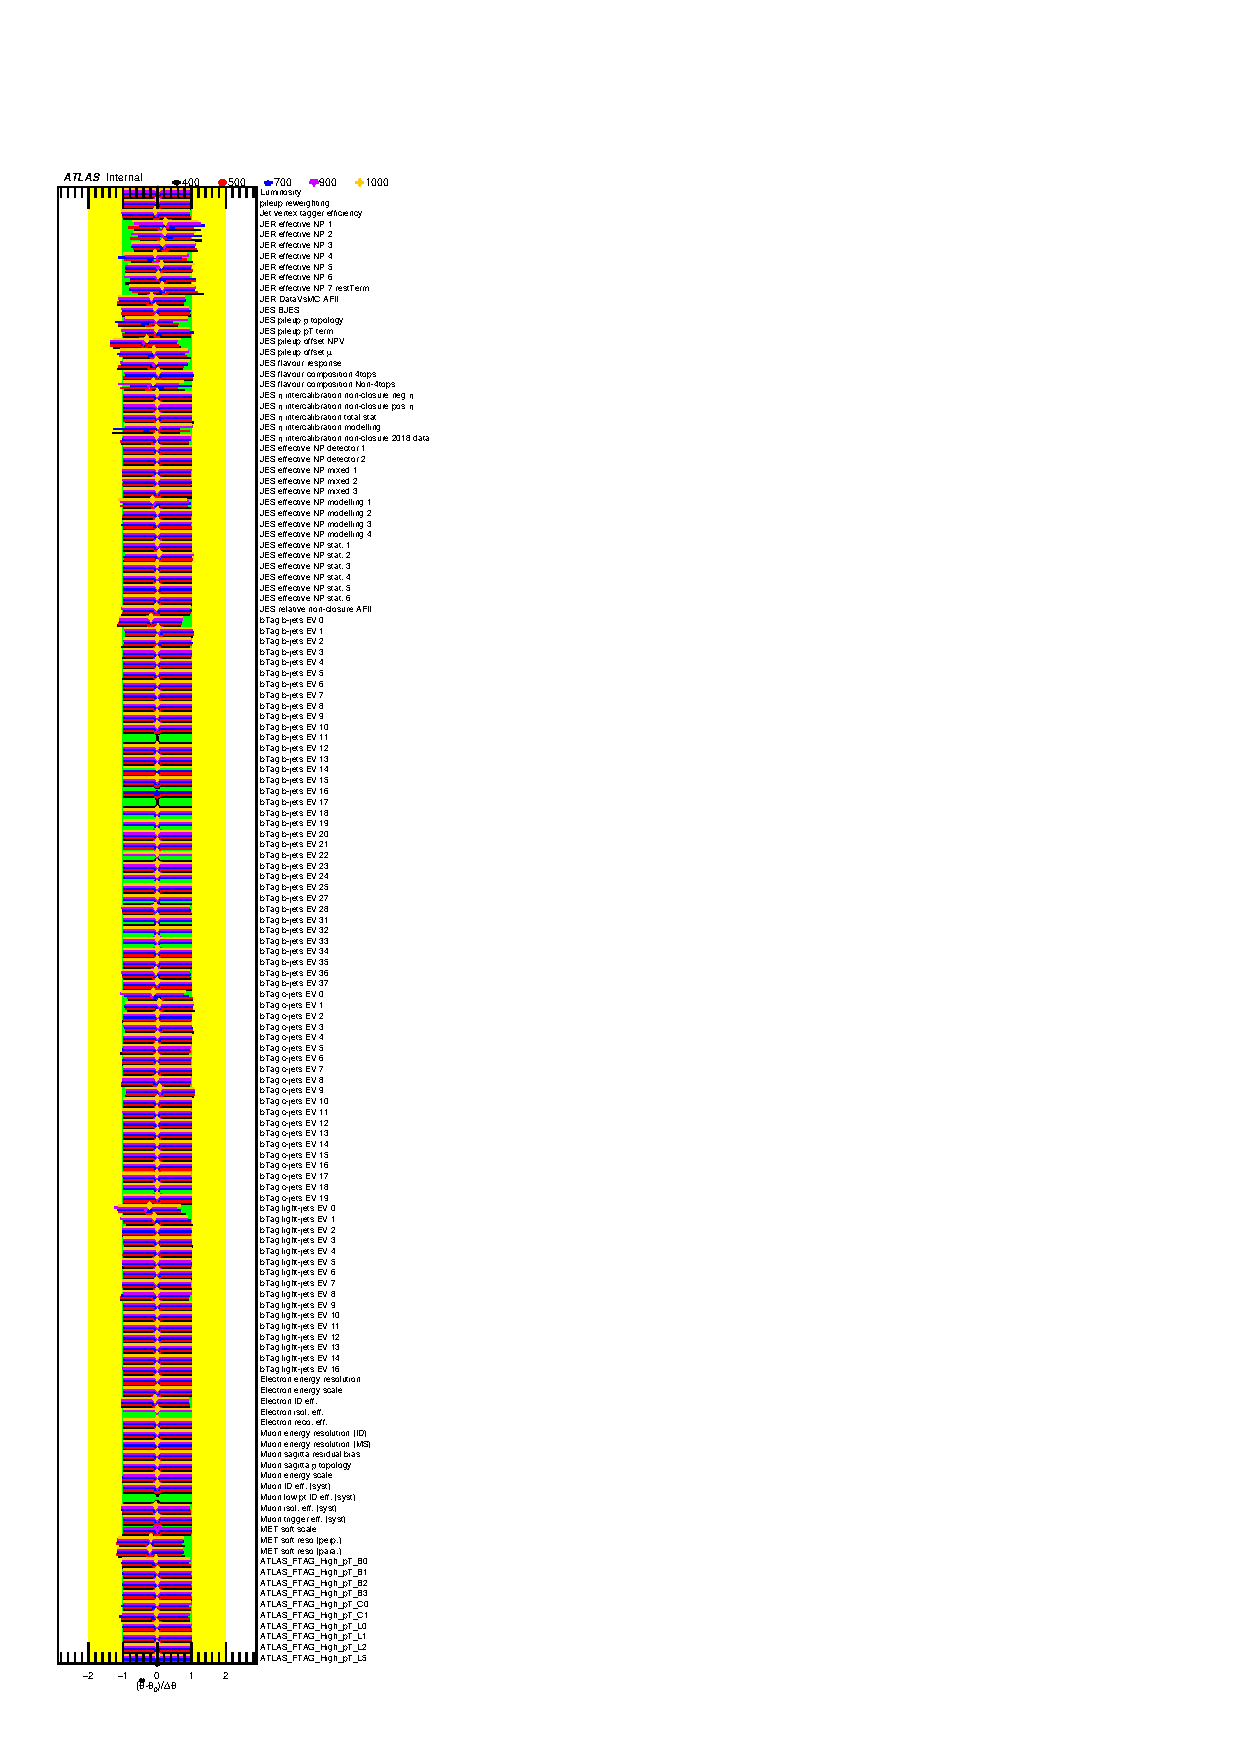
\includegraphics[width=\linewidth]{figures/fits/comparisons/massPoints/GNN/all/data/NuisPar_comp_Instrumental.pdf}
    \subcaption{1L+2L}
    \label{fig:data_NP_all_instrumental}
  \end{subfigure}
  \caption{Fitted pulls and constraints for the nuisance parameters corresponding to the instrumental systematic uncertainties for the blinded Data fit for three types of fits: using only 1L regions, using only 2L regions, and using all regions. Comparison is done for five mass points.}
\label{fig:data_NP_mass_instrumental}
\end{figure}


\begin{figure}[htbp!]
  \centering
  \begin{subfigure}[t]{0.32\textwidth}
    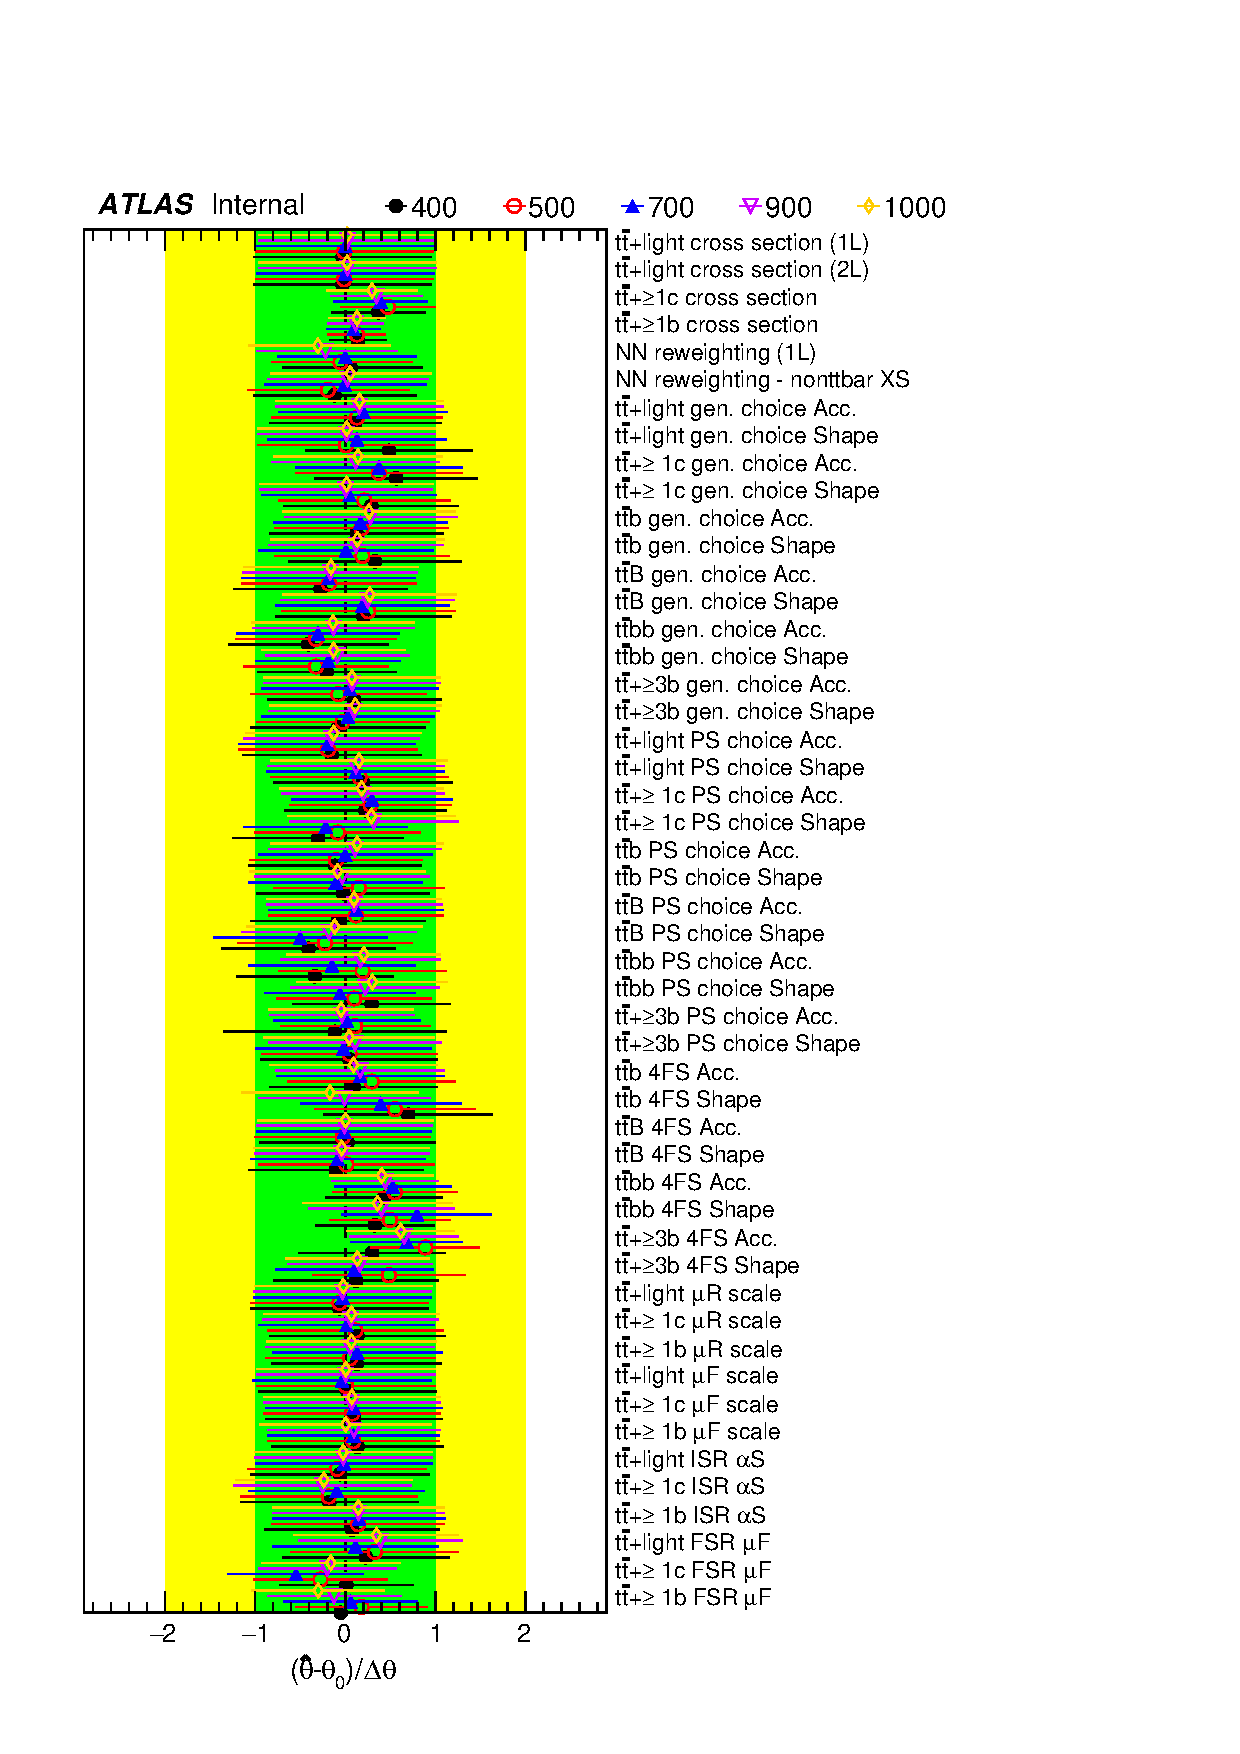
\includegraphics[width=\linewidth]{figures/fits/comparisons/massPoints/GNN/1L/data/NuisPar_comp_ttbar.pdf}
    \subcaption{1L}
    \label{fig:data_NP_1L}
  \end{subfigure}
  \begin{subfigure}[t]{0.32\textwidth}
    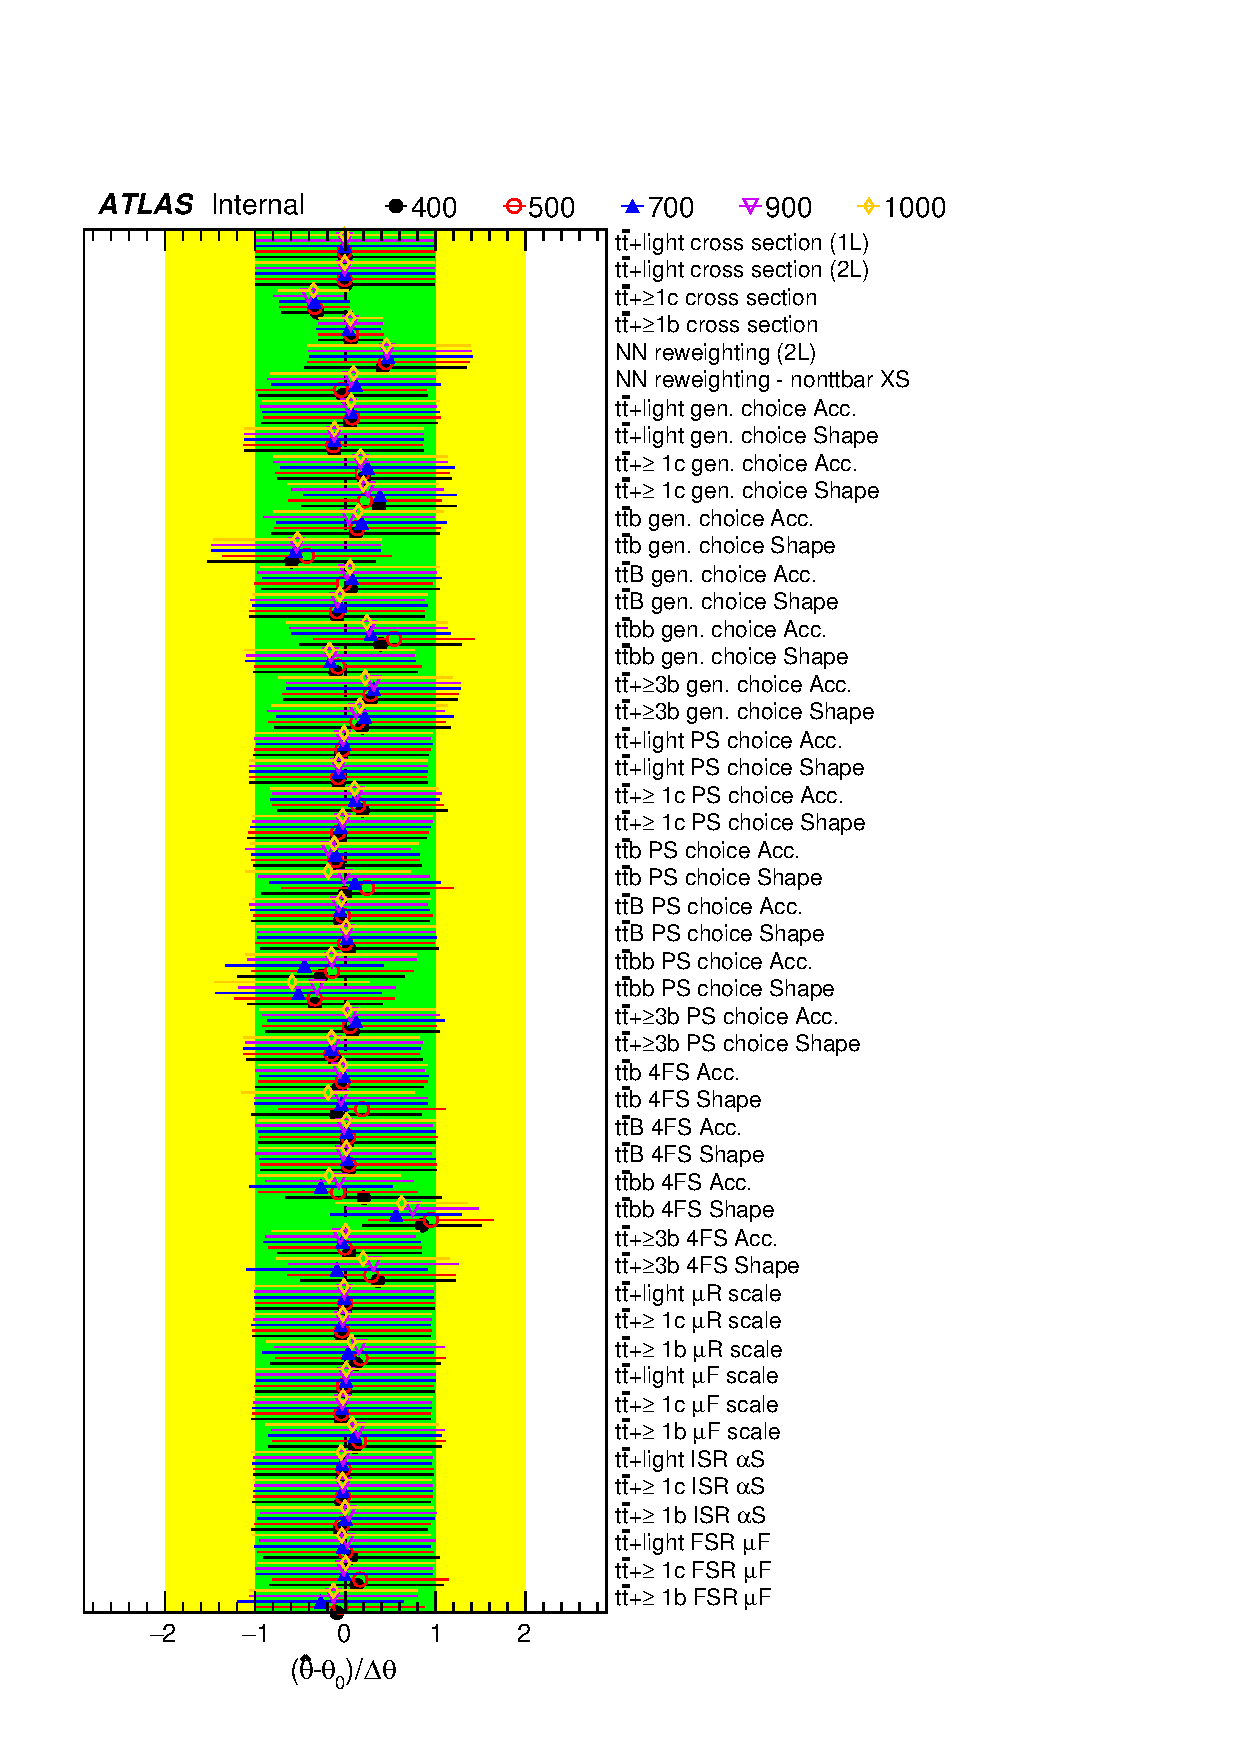
\includegraphics[width=\linewidth]{figures/fits/comparisons/massPoints/GNN/2L/data/NuisPar_comp_ttbar.pdf}
    \subcaption{2L}
    \label{fig:data_NP_2L}
  \end{subfigure}
  \begin{subfigure}[t]{0.32\textwidth}
    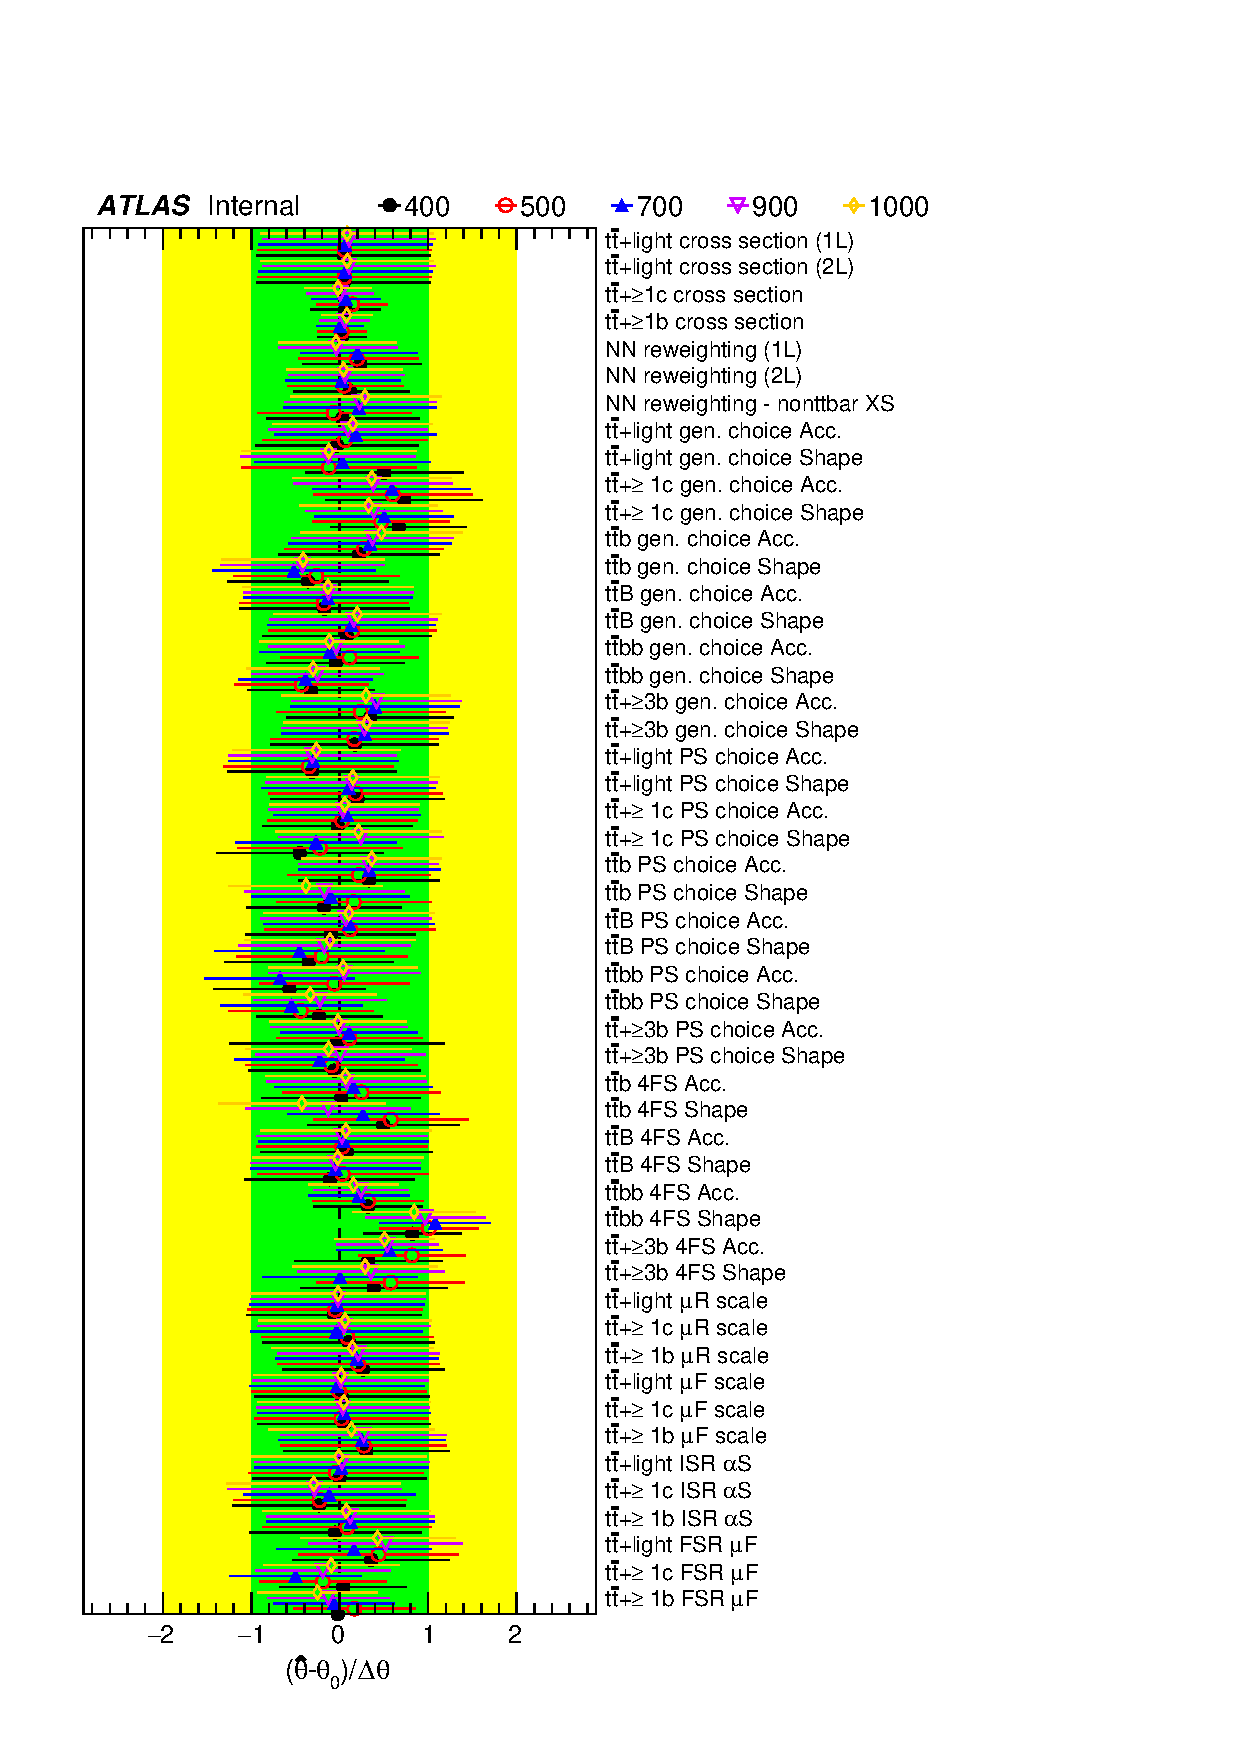
\includegraphics[width=\linewidth]{figures/fits/comparisons/massPoints/GNN/all/data/NuisPar_comp_ttbar.pdf}
    \subcaption{1L+2L}
    \label{fig:data_NP_all}
  \end{subfigure}
  \caption{Fitted pulls and constraints for the nuisance parameters corresponding to the \ttbar systematic uncertainties for the blinded Data fit for three types of fits: using only 1L regions, using only 2L regions, and using all regions. Comparison is done for five mass points.}
\label{fig:data_NP_mass_ttbar}
\end{figure}


\begin{figure}[htbp!]
  \centering
  \begin{subfigure}[t]{0.32\textwidth}
    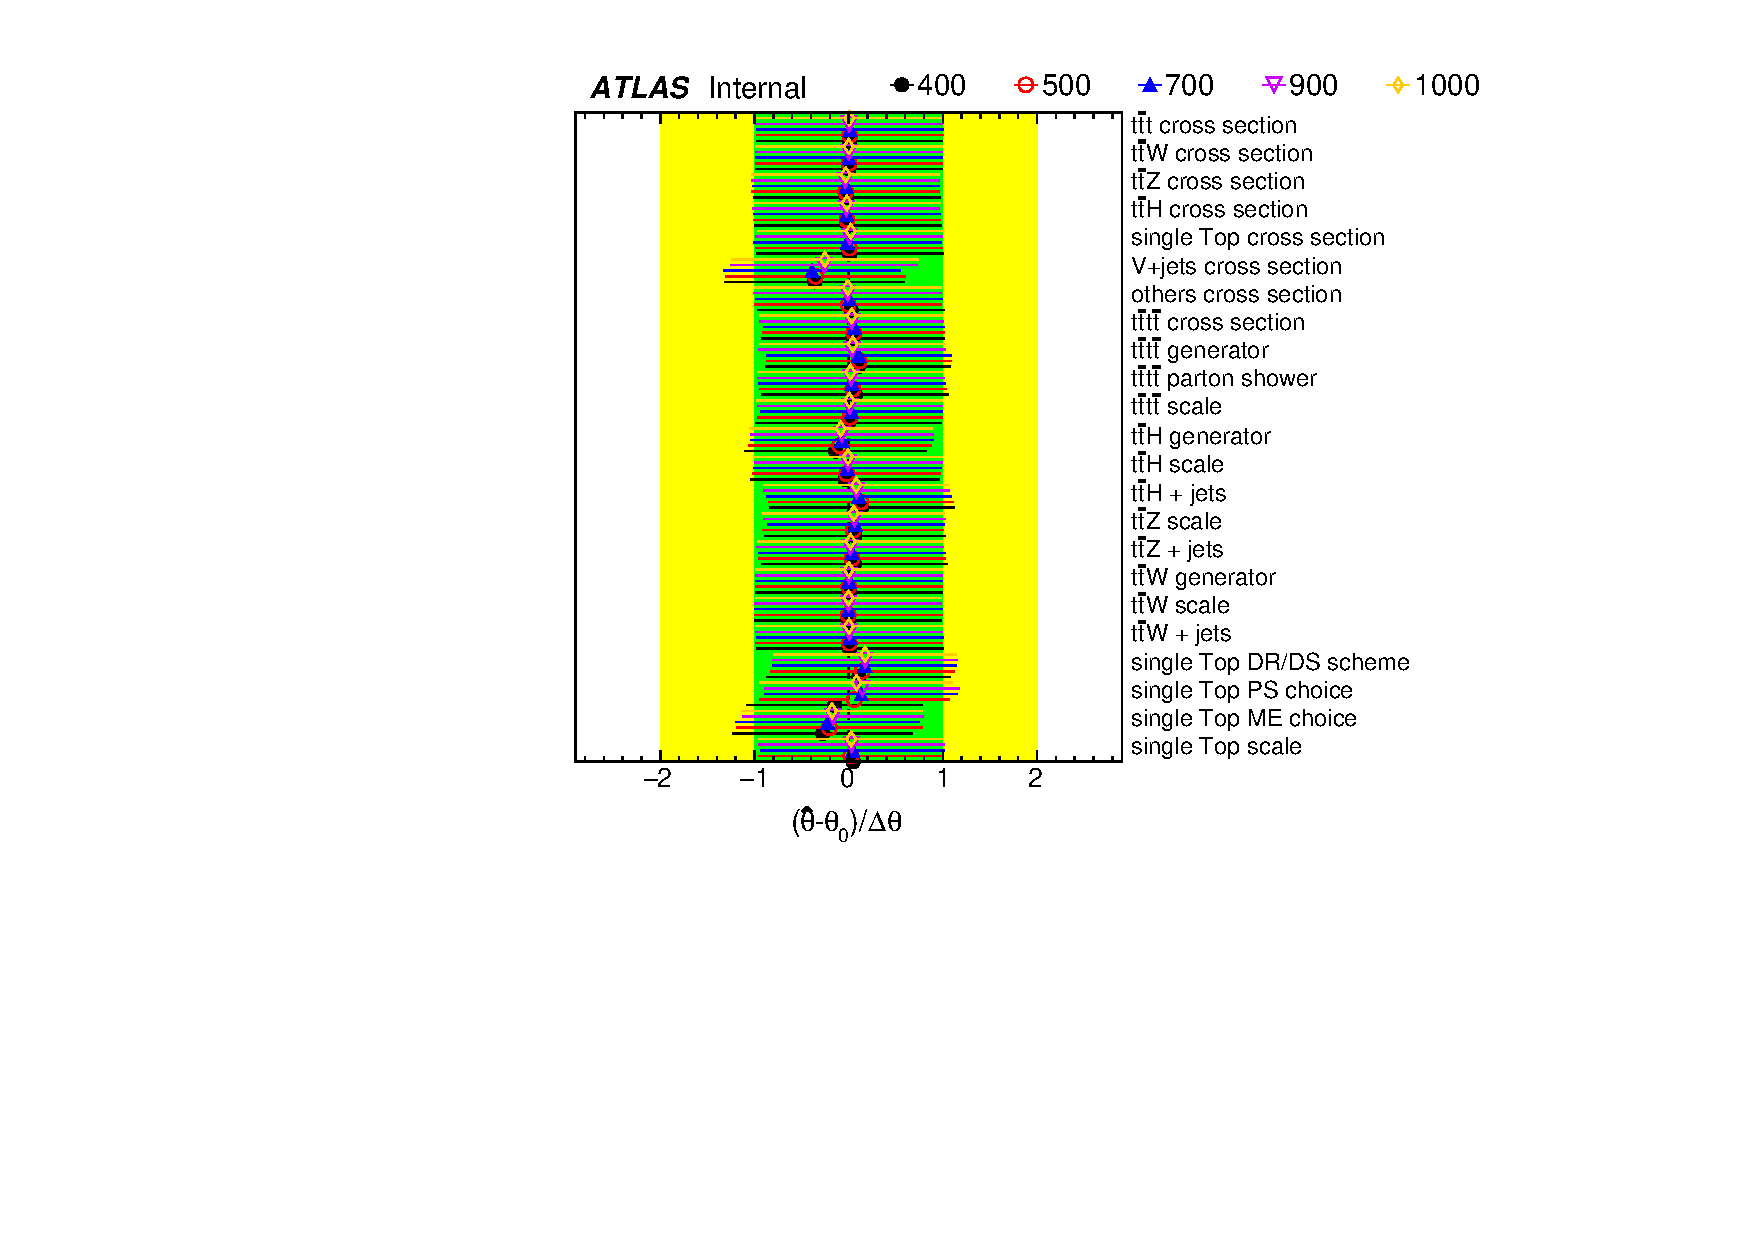
\includegraphics[width=\linewidth]{figures/fits/comparisons/massPoints/GNN/1L/data/NuisPar_comp_Other.pdf}
    \subcaption{1L}
    \label{fig:data_NP_1L_other}
  \end{subfigure}
  \begin{subfigure}[t]{0.32\textwidth}
    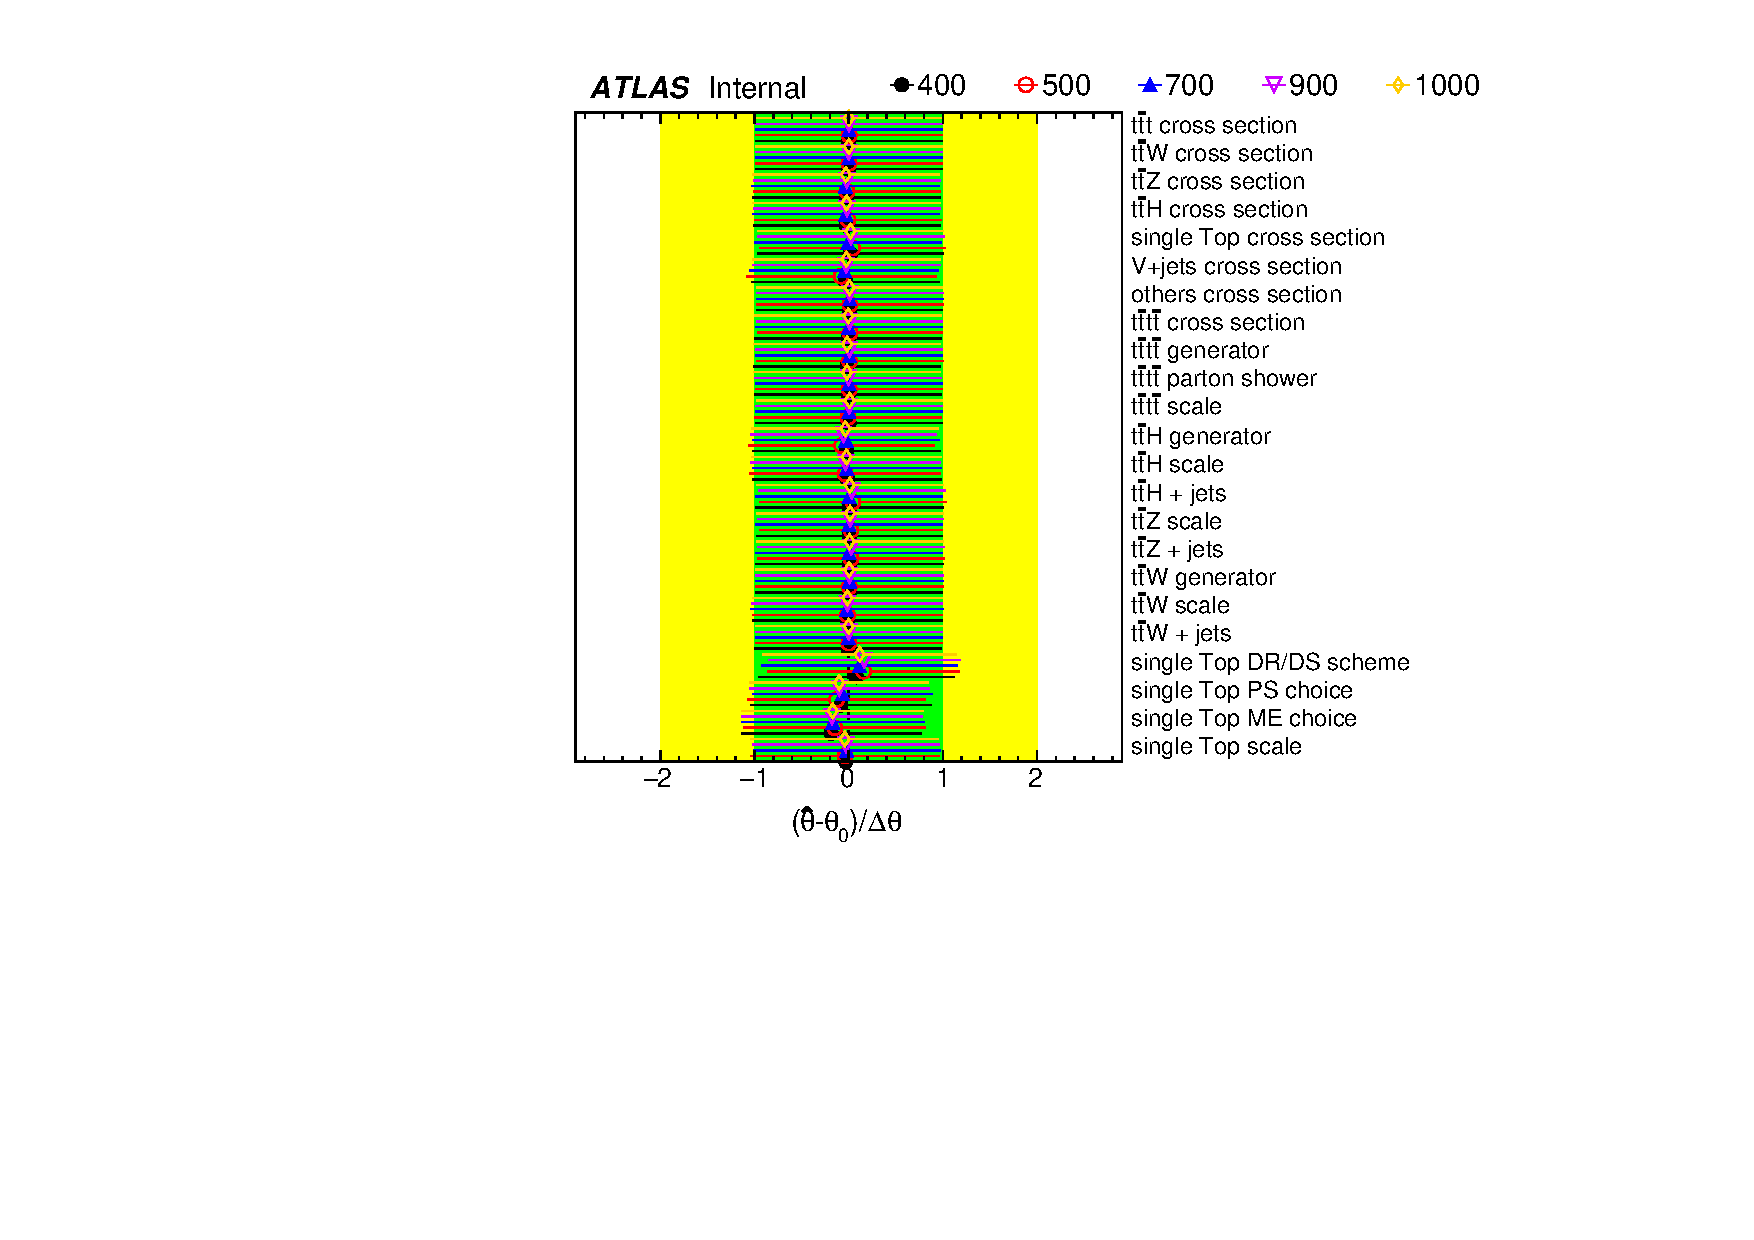
\includegraphics[width=\linewidth]{figures/fits/comparisons/massPoints/GNN/2L/data/NuisPar_comp_Other.pdf}
    \subcaption{2L}
    \label{fig:data_NP_2L_other}
  \end{subfigure}
  \begin{subfigure}[t]{0.32\textwidth}
    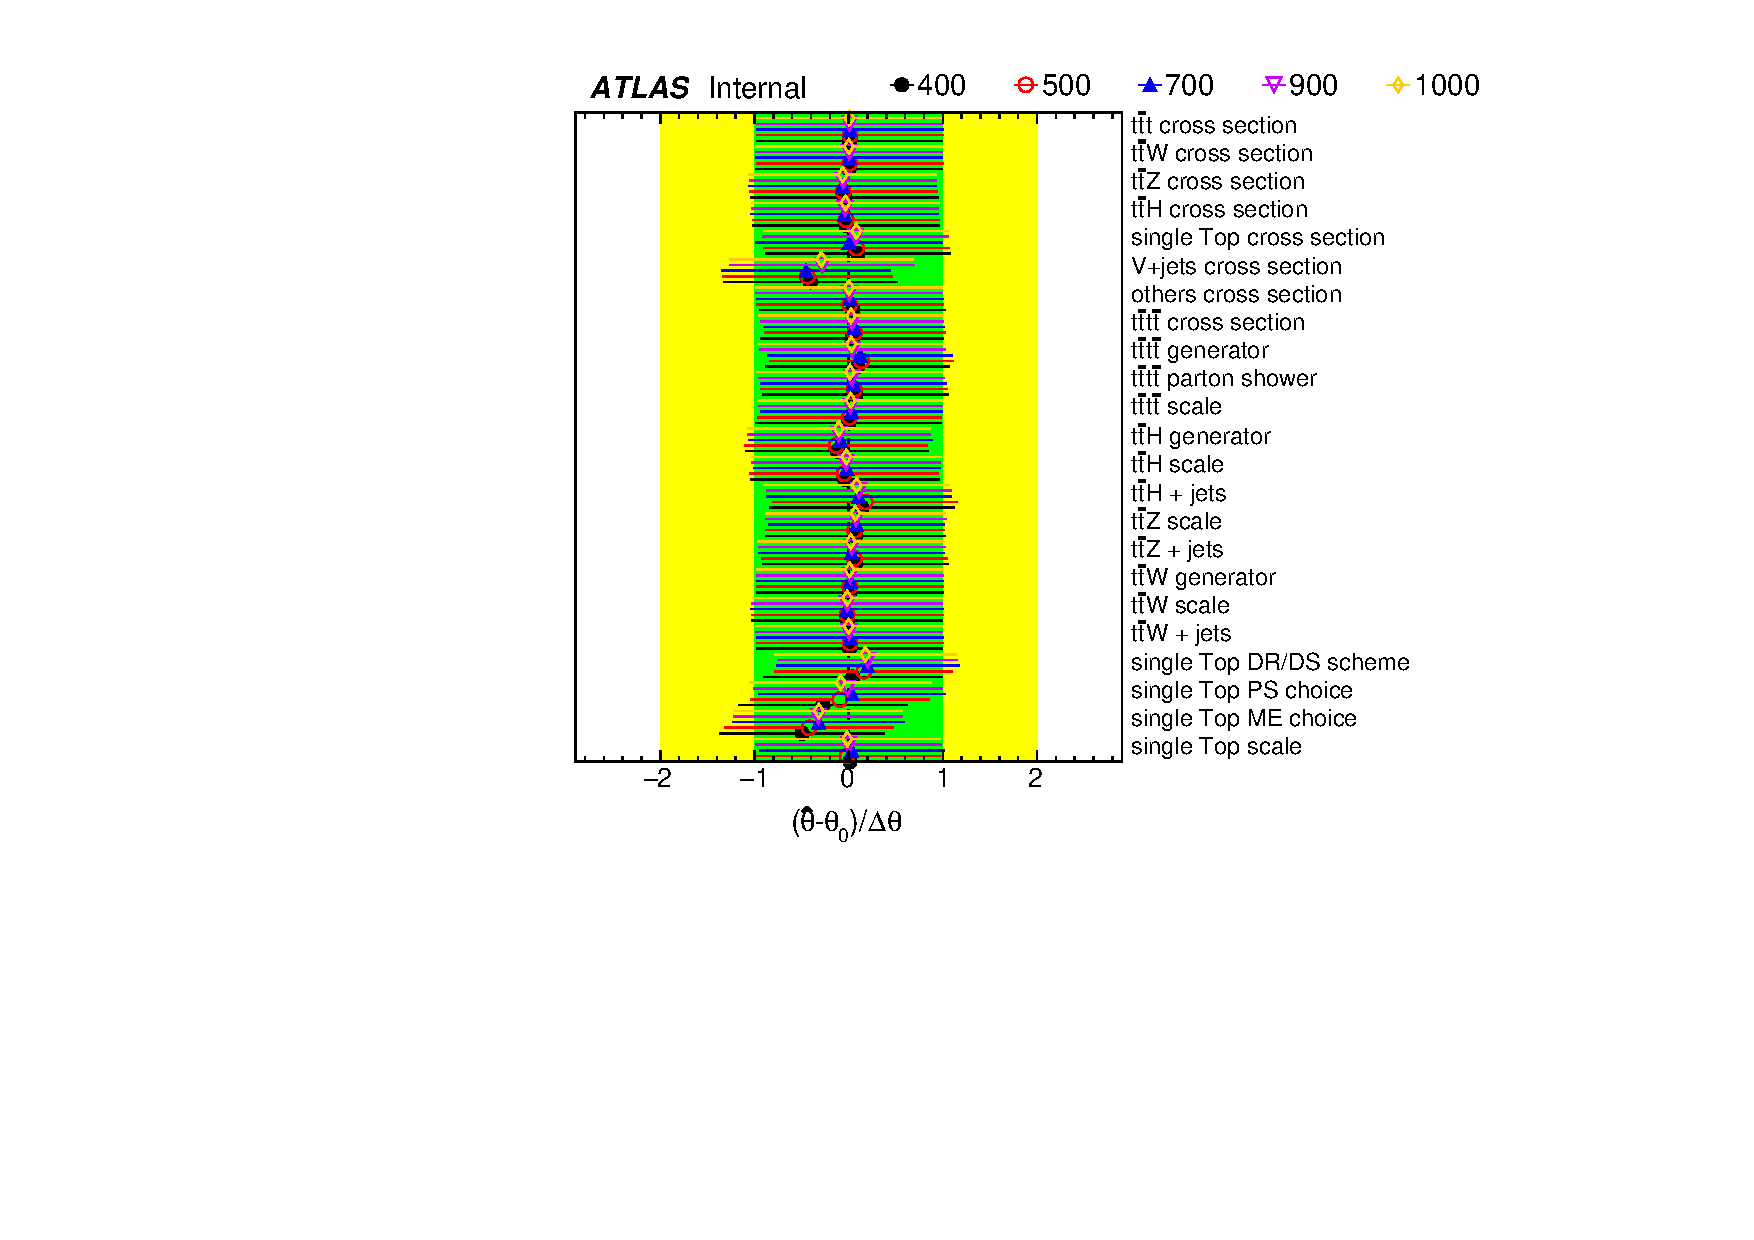
\includegraphics[width=\linewidth]{figures/fits/comparisons/massPoints/GNN/all/data/NuisPar_comp_Other.pdf}
    \subcaption{1L+2L}
    \label{fig:data_NP_all_other}
  \end{subfigure}
  \caption{Fitted pulls and constraints for the nuisance parameters corresponding to the non-\ttbar-background systematic uncertainties for the blinded Data fit for three types of fits: using only 1L regions, using only 2L regions, and using all regions. Comparison is done for five mass points.}
\label{fig:data_NP_mass_other}
\end{figure}


\begin{figure}[htbp!]
        \centering
        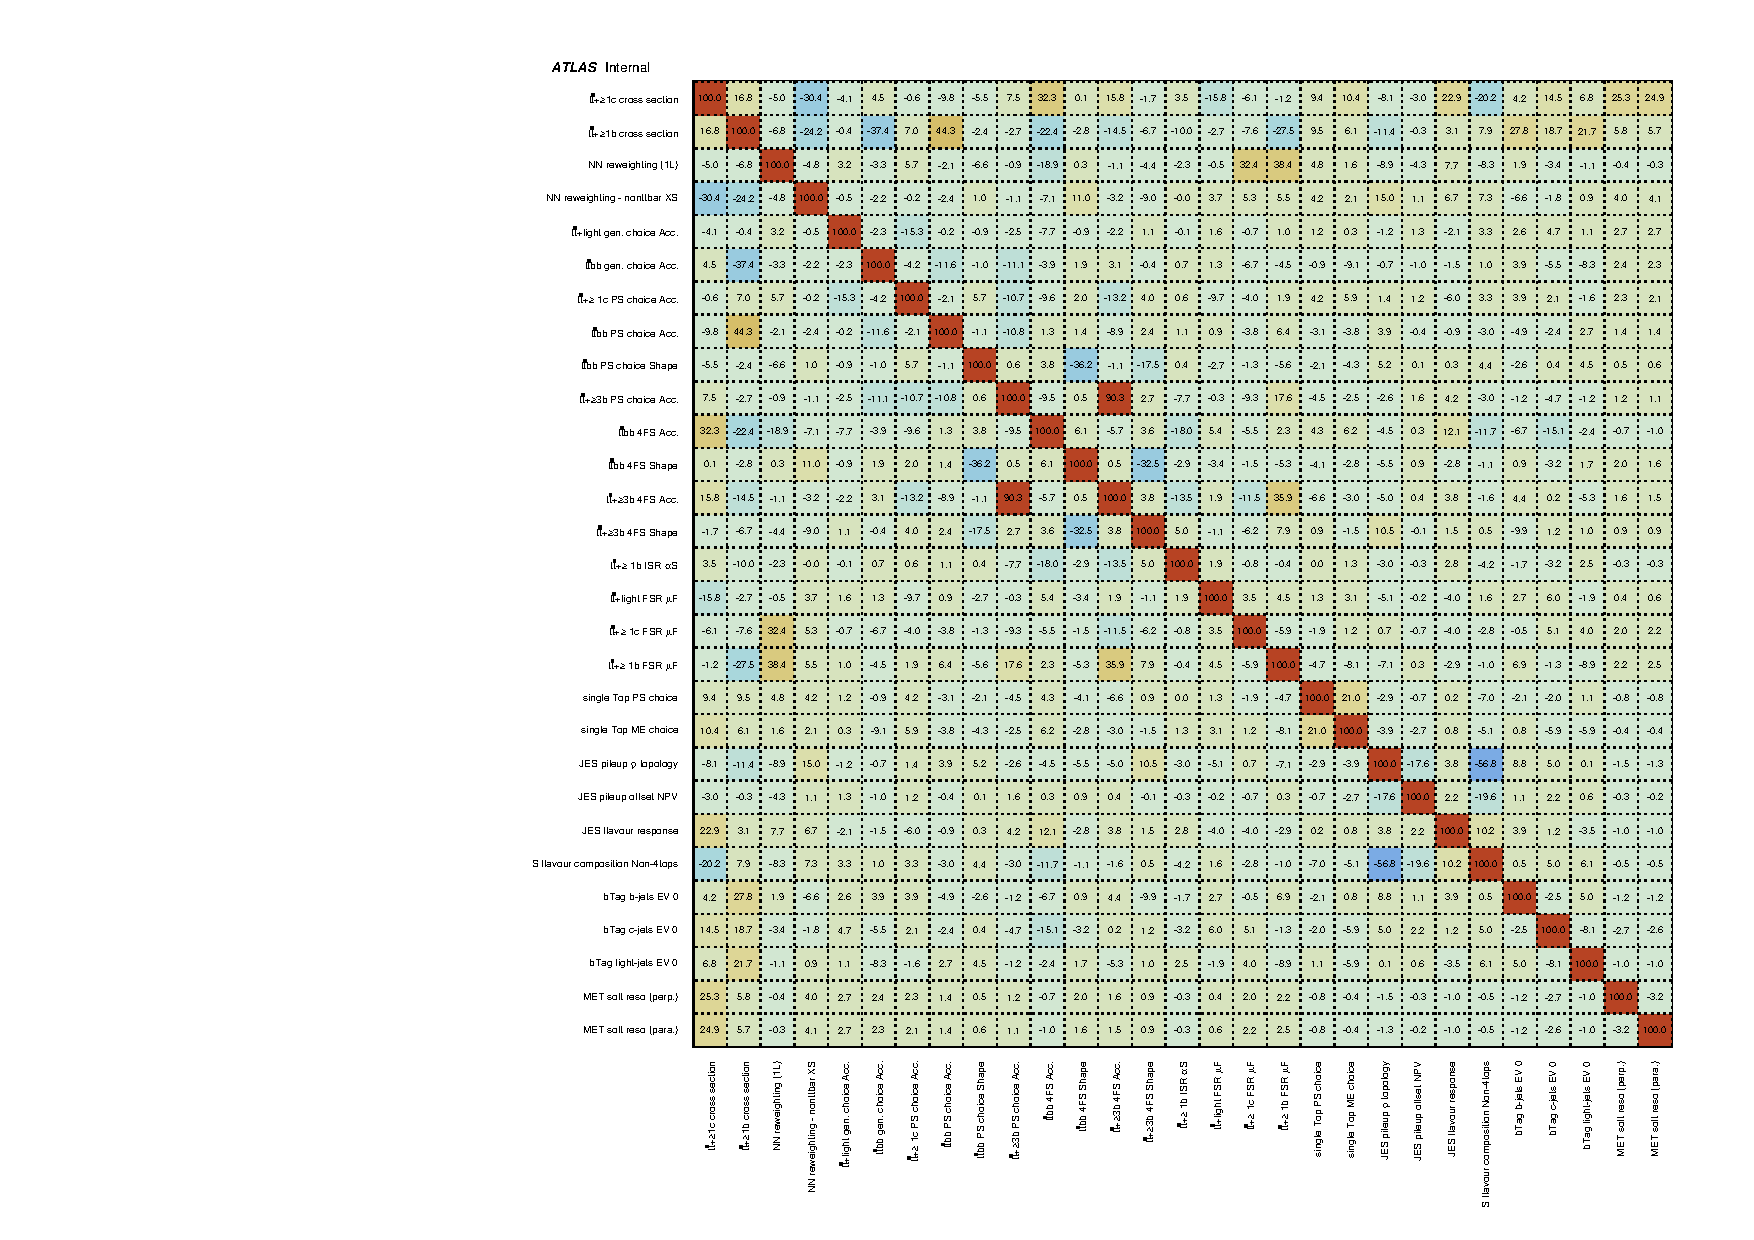
\includegraphics[width=\linewidth]{figures/fits/GNN/400/1L/data/CorrMatrix.pdf}
        \caption{\label{fig:Corr_mH400_Data_1L}Correlation matrix for the 1L blinded data fit for mH = 400 GeV}
\end{figure}

\begin{figure}[htbp!]
        \centering
        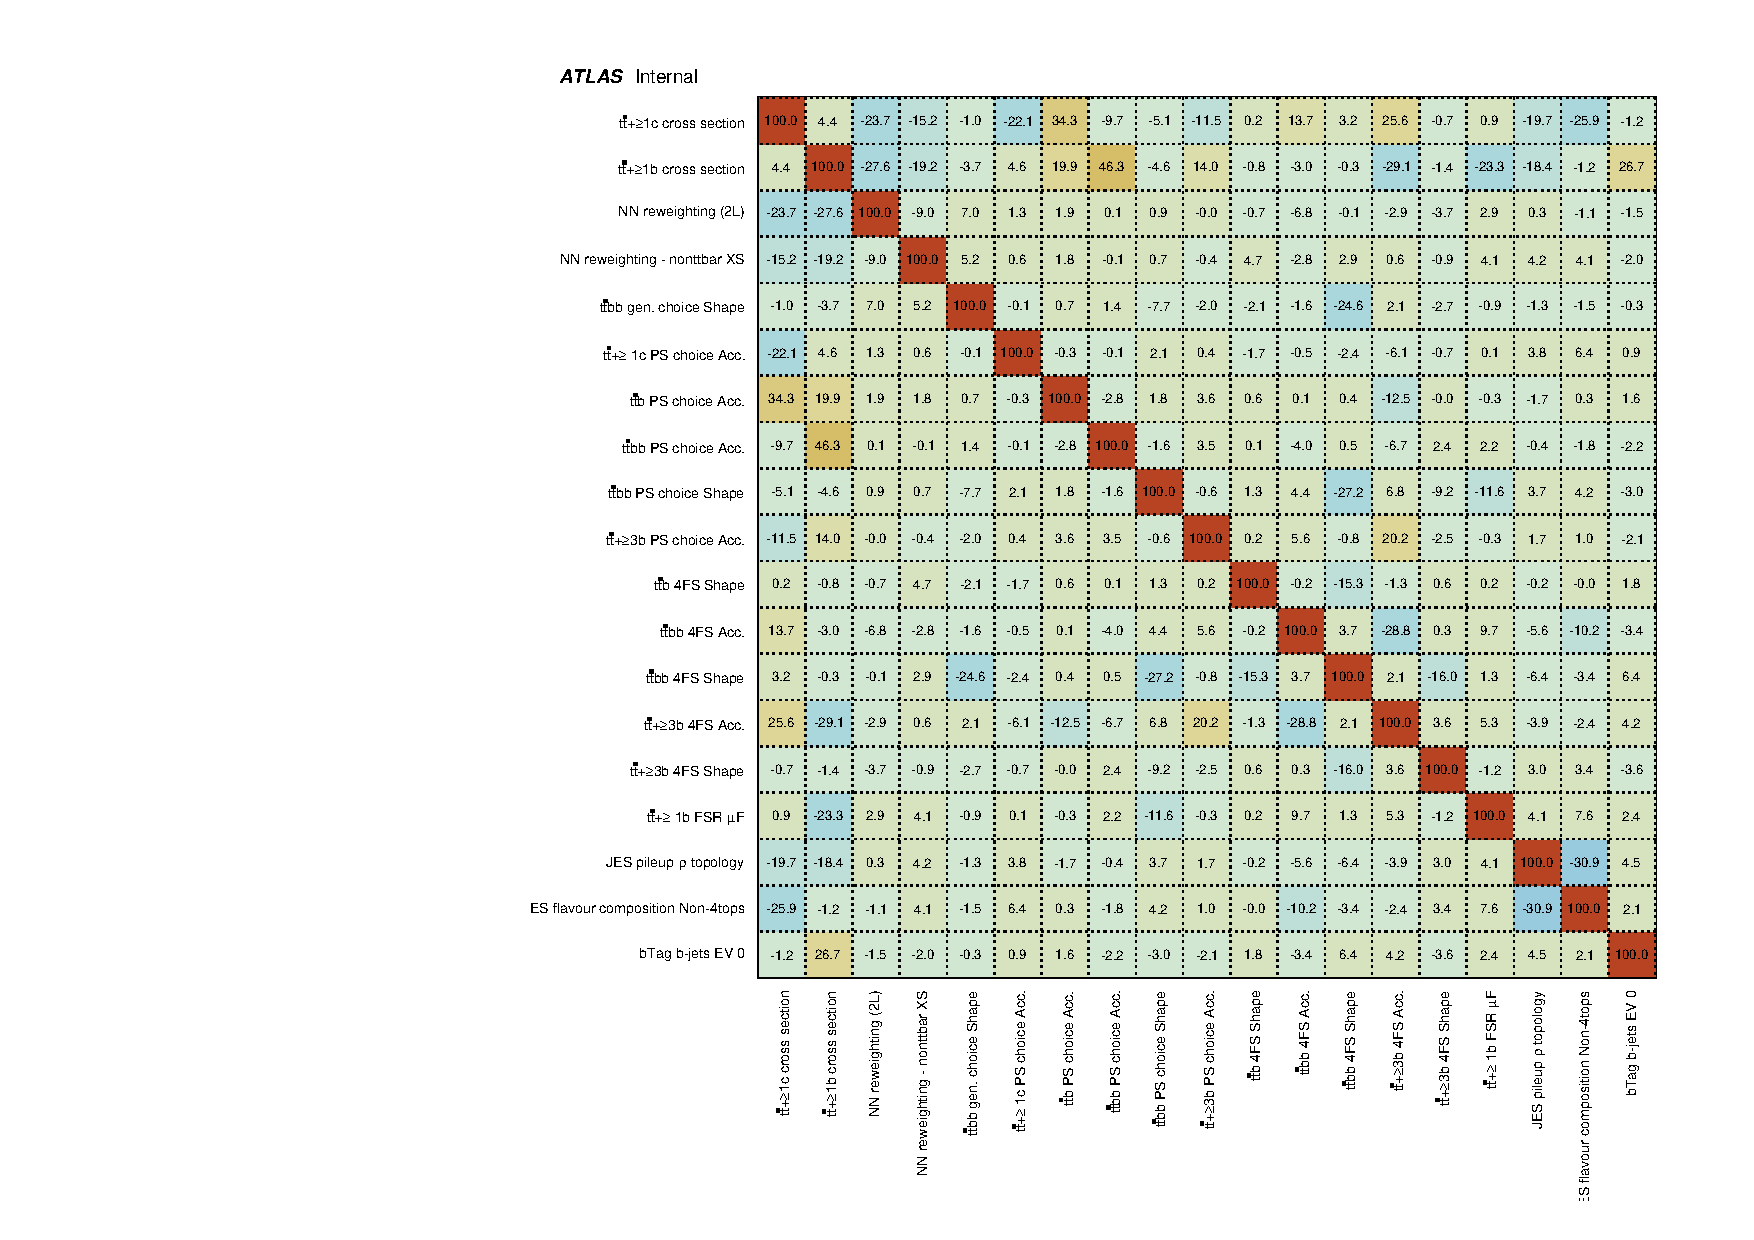
\includegraphics[width=\linewidth]{figures/fits/GNN/400/2L/data/CorrMatrix.pdf}
        \caption{\label{fig:Corr_mH400_Data_2L}Correlation matrix for the 2LOS blinded data fit for mH = 400 GeV}
\end{figure}

\begin{figure}[htbp!]
        \centering
        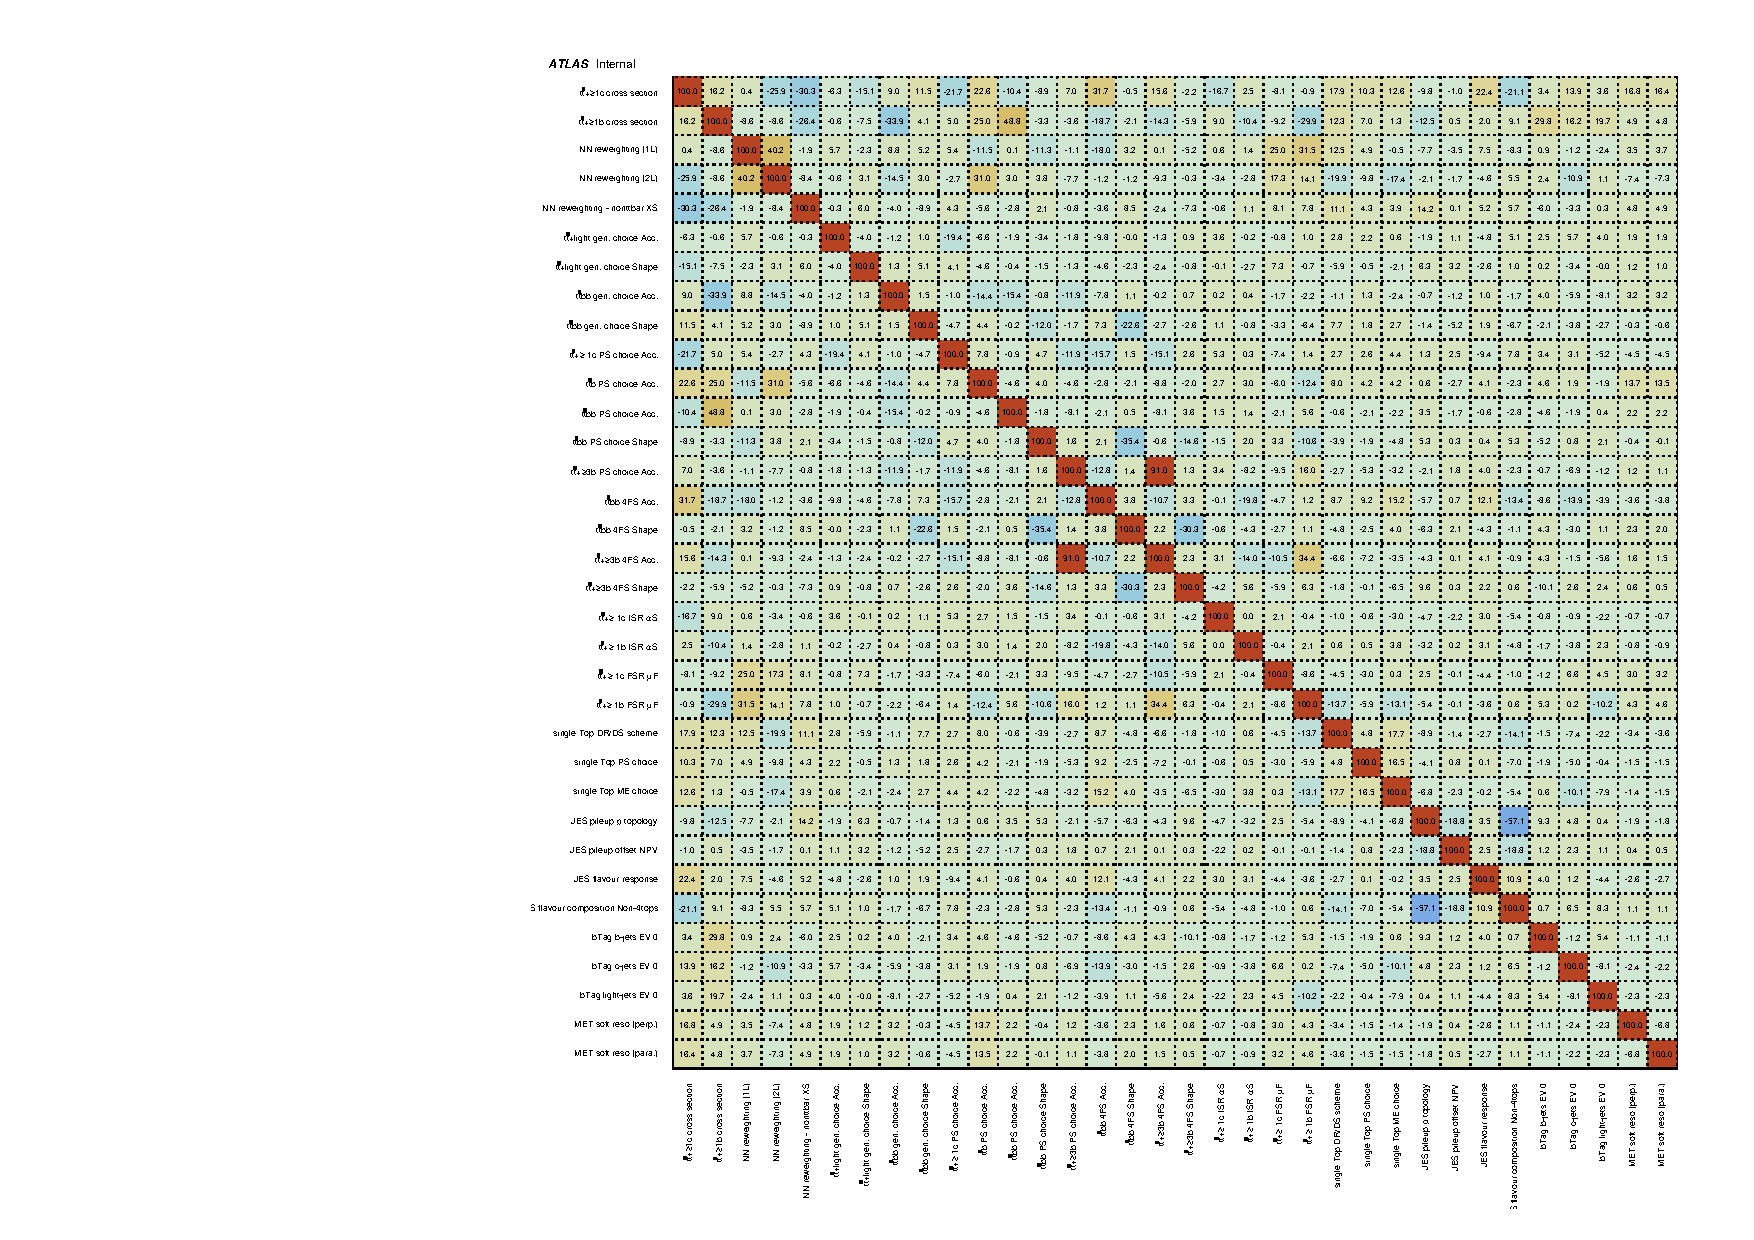
\includegraphics[width=\linewidth]{figures/fits/GNN/400/all/data/CorrMatrix.pdf}
        \caption{\label{fig:Corr_mH400_Data_all}Correlation matrix for the 1L/2LOS combined blinded data fit for mH = 400 GeV}
\end{figure}

%-------------------------------------------------------------------------------

%-------------------------------------------------------------------------------
\FloatBarrier
\section{Fits to unblinded data - background only}% Peter
\label{sec:unblinded_Bonly}
A fit using data is performed on using all bins, without blinding. The signal sample is not included in the fit (it is a background-only fit). The unblinded data fit is performed over all control and signal regions (combined 1L+2LOS), and with all available samples and systematics. The dominant ttbar background is reweighted using the NN method.

The post-fit distributions associated with each background and signal region are shown in Figure \ref{fig:unblinded_data_Bonly_postfit_1L} for 1L regions and Figure \ref{fig:unblinded_data_Bonly_postfit_2L} for 2LOS regions from the combined fit using mass point $m_H=400$ GeV. The nuisance parameter pulls and constraints are compared between 1L, 2LOS, and the combined fit in Figures \ref{fig:unblinded_data_Bonly_NP_instrumental}, \ref{fig:unblinded_data_Bonly_NP_ttbar}, and \ref{fig:unblinded_data_Bonly_NP_other}. Comparison for the fits using GNN outputs trained on various mass points are shown in Figures \ref{fig:unblinded_data_Bonly_NP_mass_instrumental}, \ref{fig:unblinded_data_Bonly_NP_mass_ttbar}, and \ref{fig:unblinded_data_Bonly_NP_mass_other}.

Correlation matrices for systematics for 1L, 2LOS, and the combined fit are shown in Figure \ref{fig:unblinded_data_Bonly_corr_mH400_Data_1L}, Figure \ref{fig:unblinded_data_Bonly_corr_mH400_Data_2L}, and Figure \ref{fig:unblinded_data_Bonly_corr_mH400_Data_all} respectively.

The appendix \ref{app:validation_region_studies} shows post-fit plots in validation regions for 1L and 2LOS regions for $m_H=400$ GeV including all systematics. The postfit agreement is good. The appendix \ref{app:700_1000} shows pre-fit and post-fit distributions for higher mass points, $m_H=700$ and $m_H=1000$ GeV, as well as the correlation matrices.

\begin{figure}[htbp!]
        \begin{center} \setlength{\tabcolsep}{2.5pt}\footnotesize
        \begin{tabular}{cccc}
        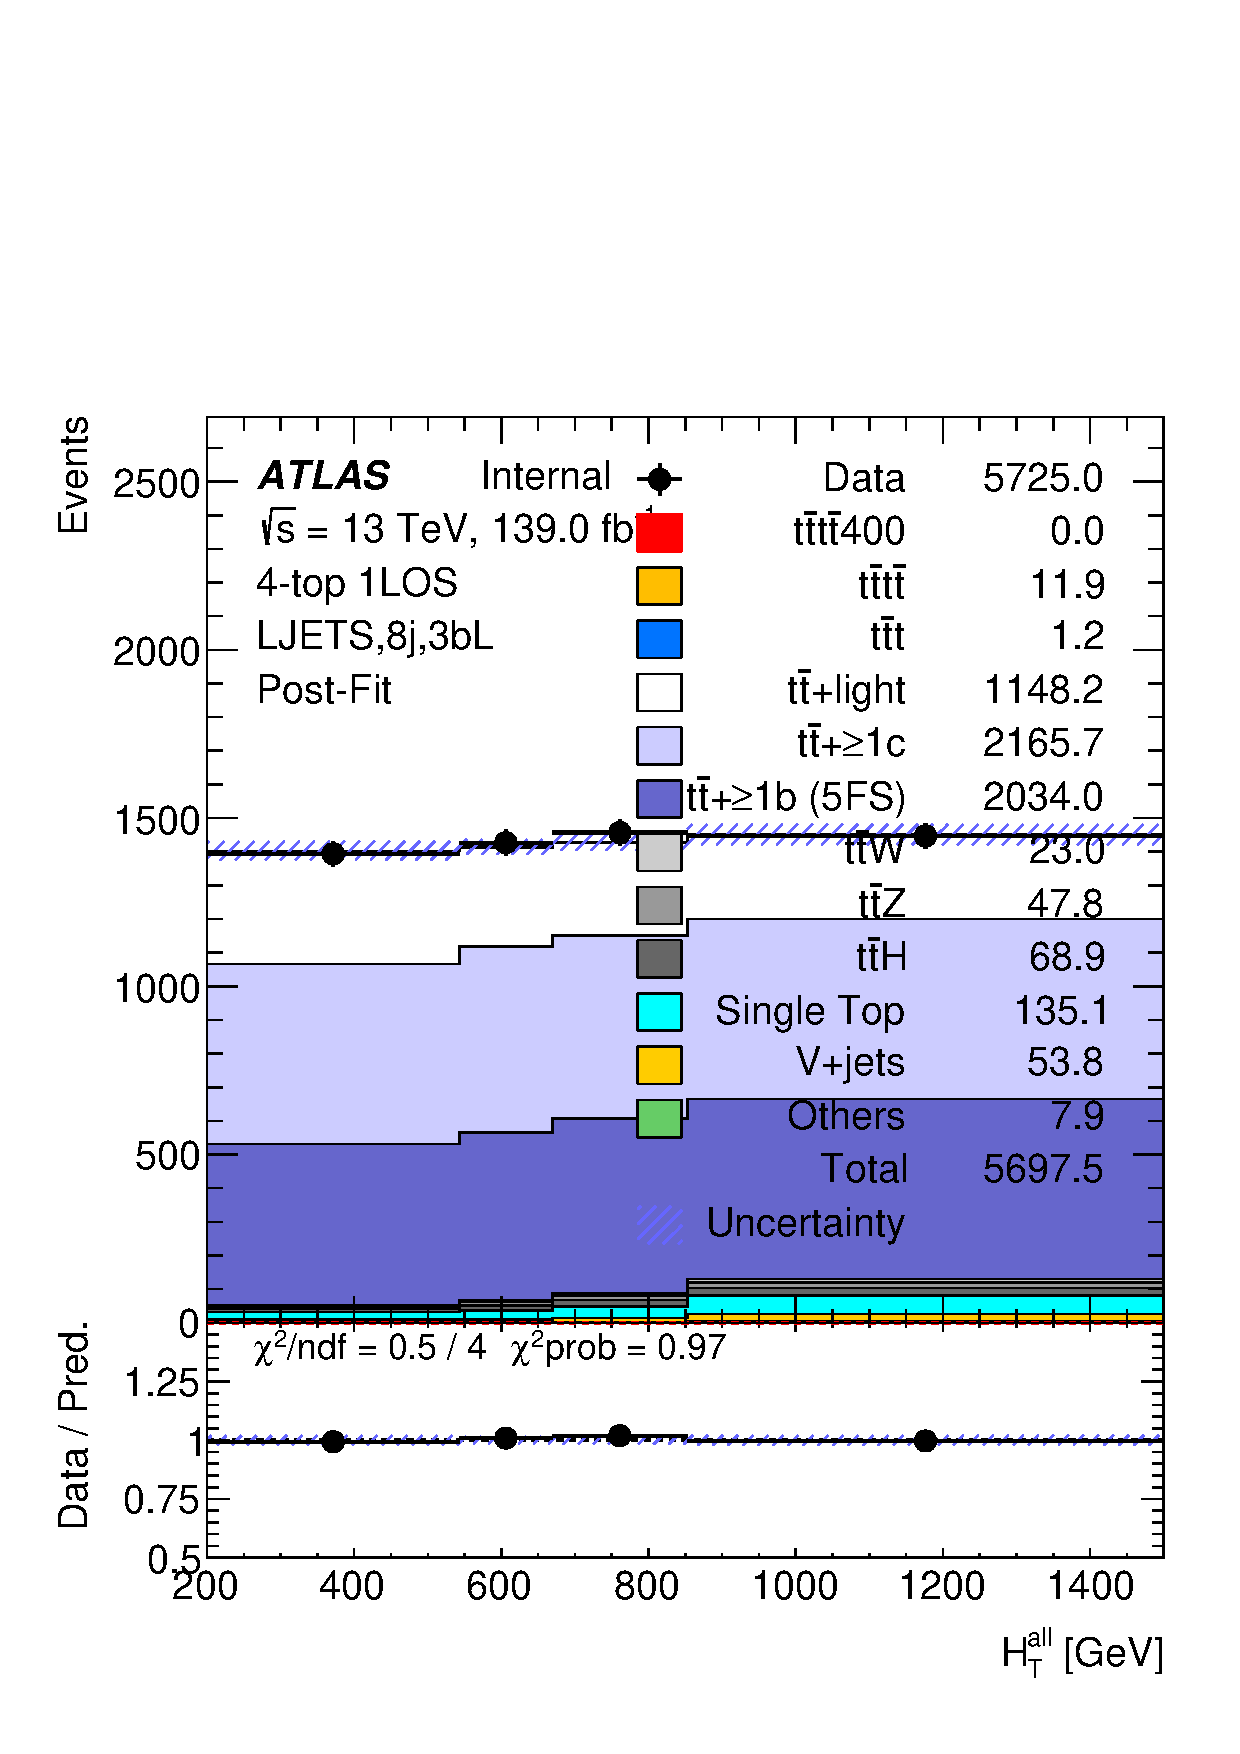
\includegraphics[width=0.23 \textwidth]{figures/fits/GNN/400/all/data_unblindedBonly/Plots/ljets_8j3bL_postFit.pdf} &
        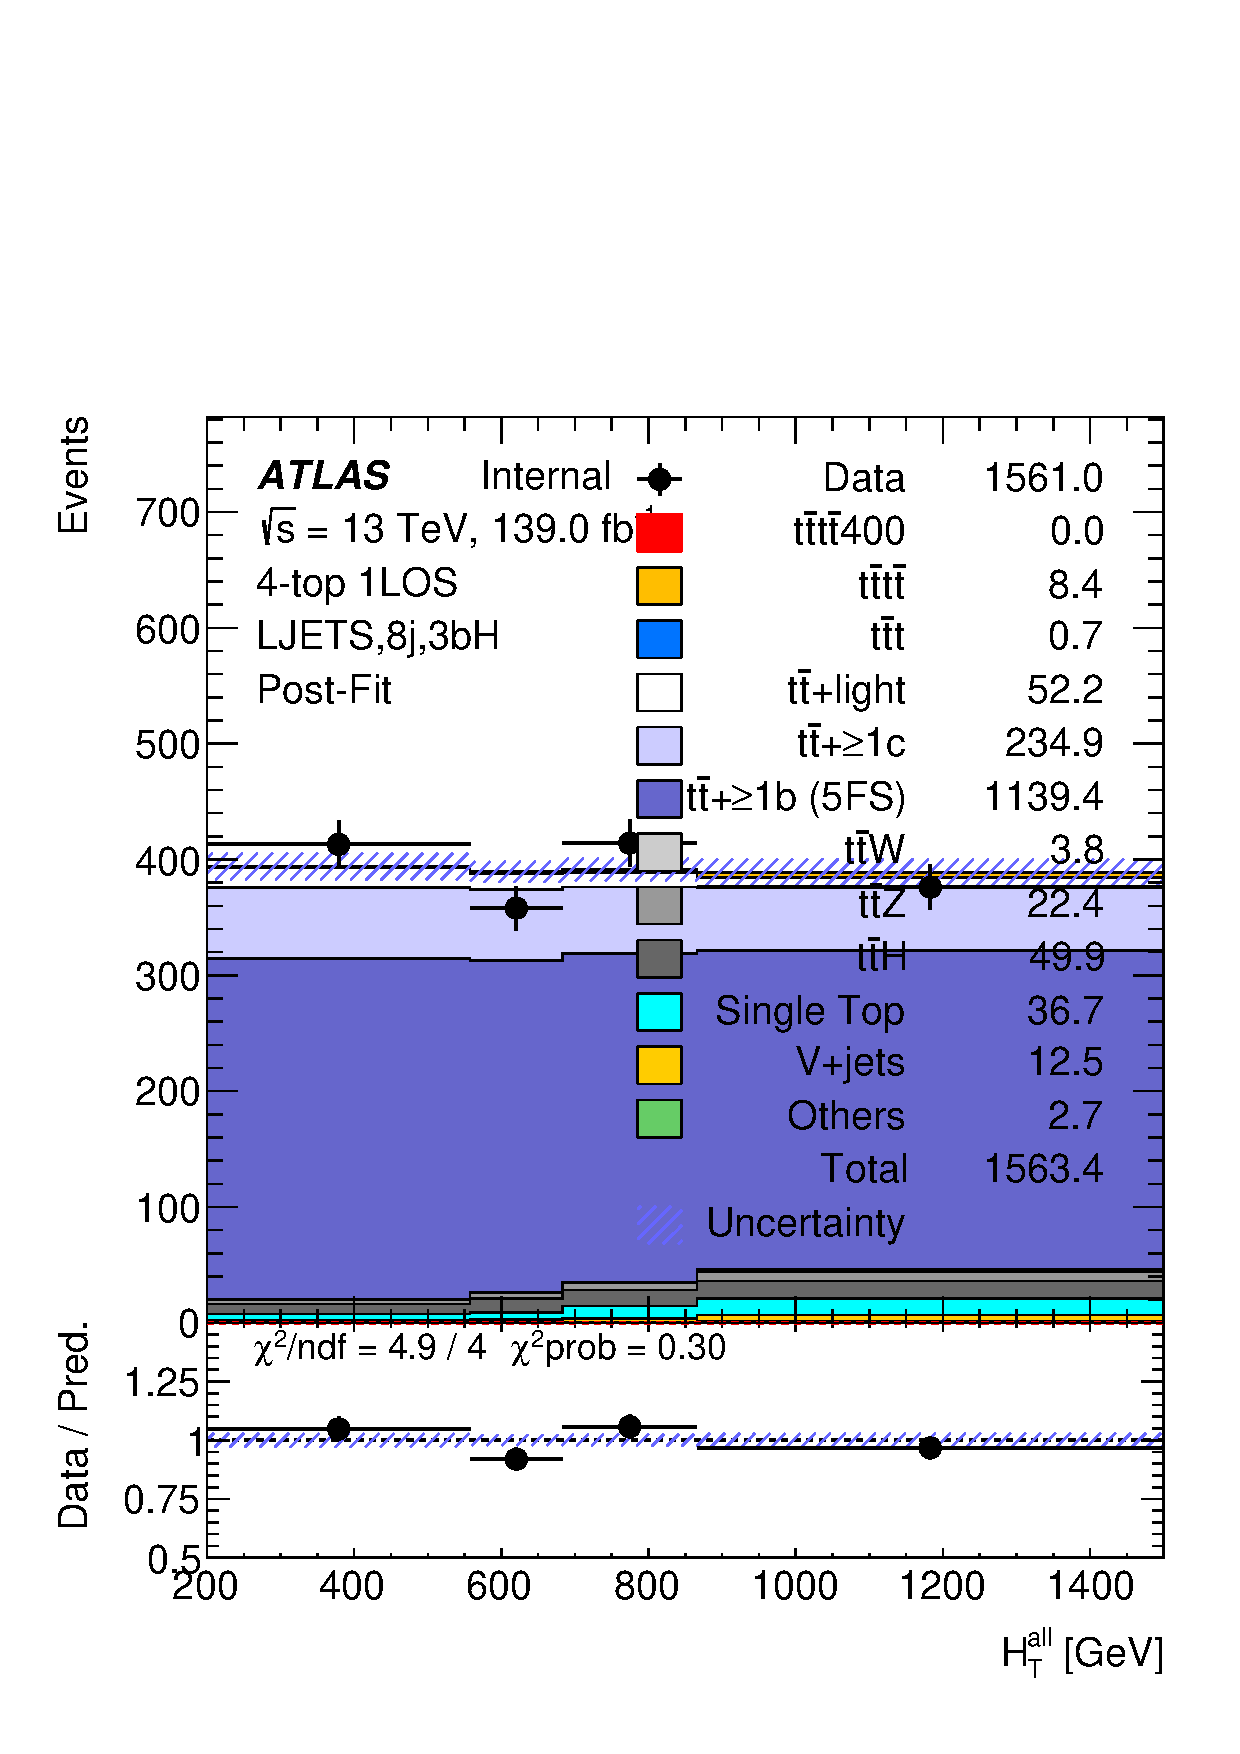
\includegraphics[width=0.23 \textwidth]{figures/fits/GNN/400/all/data_unblindedBonly/Plots/ljets_8j3bH_postFit.pdf} &
        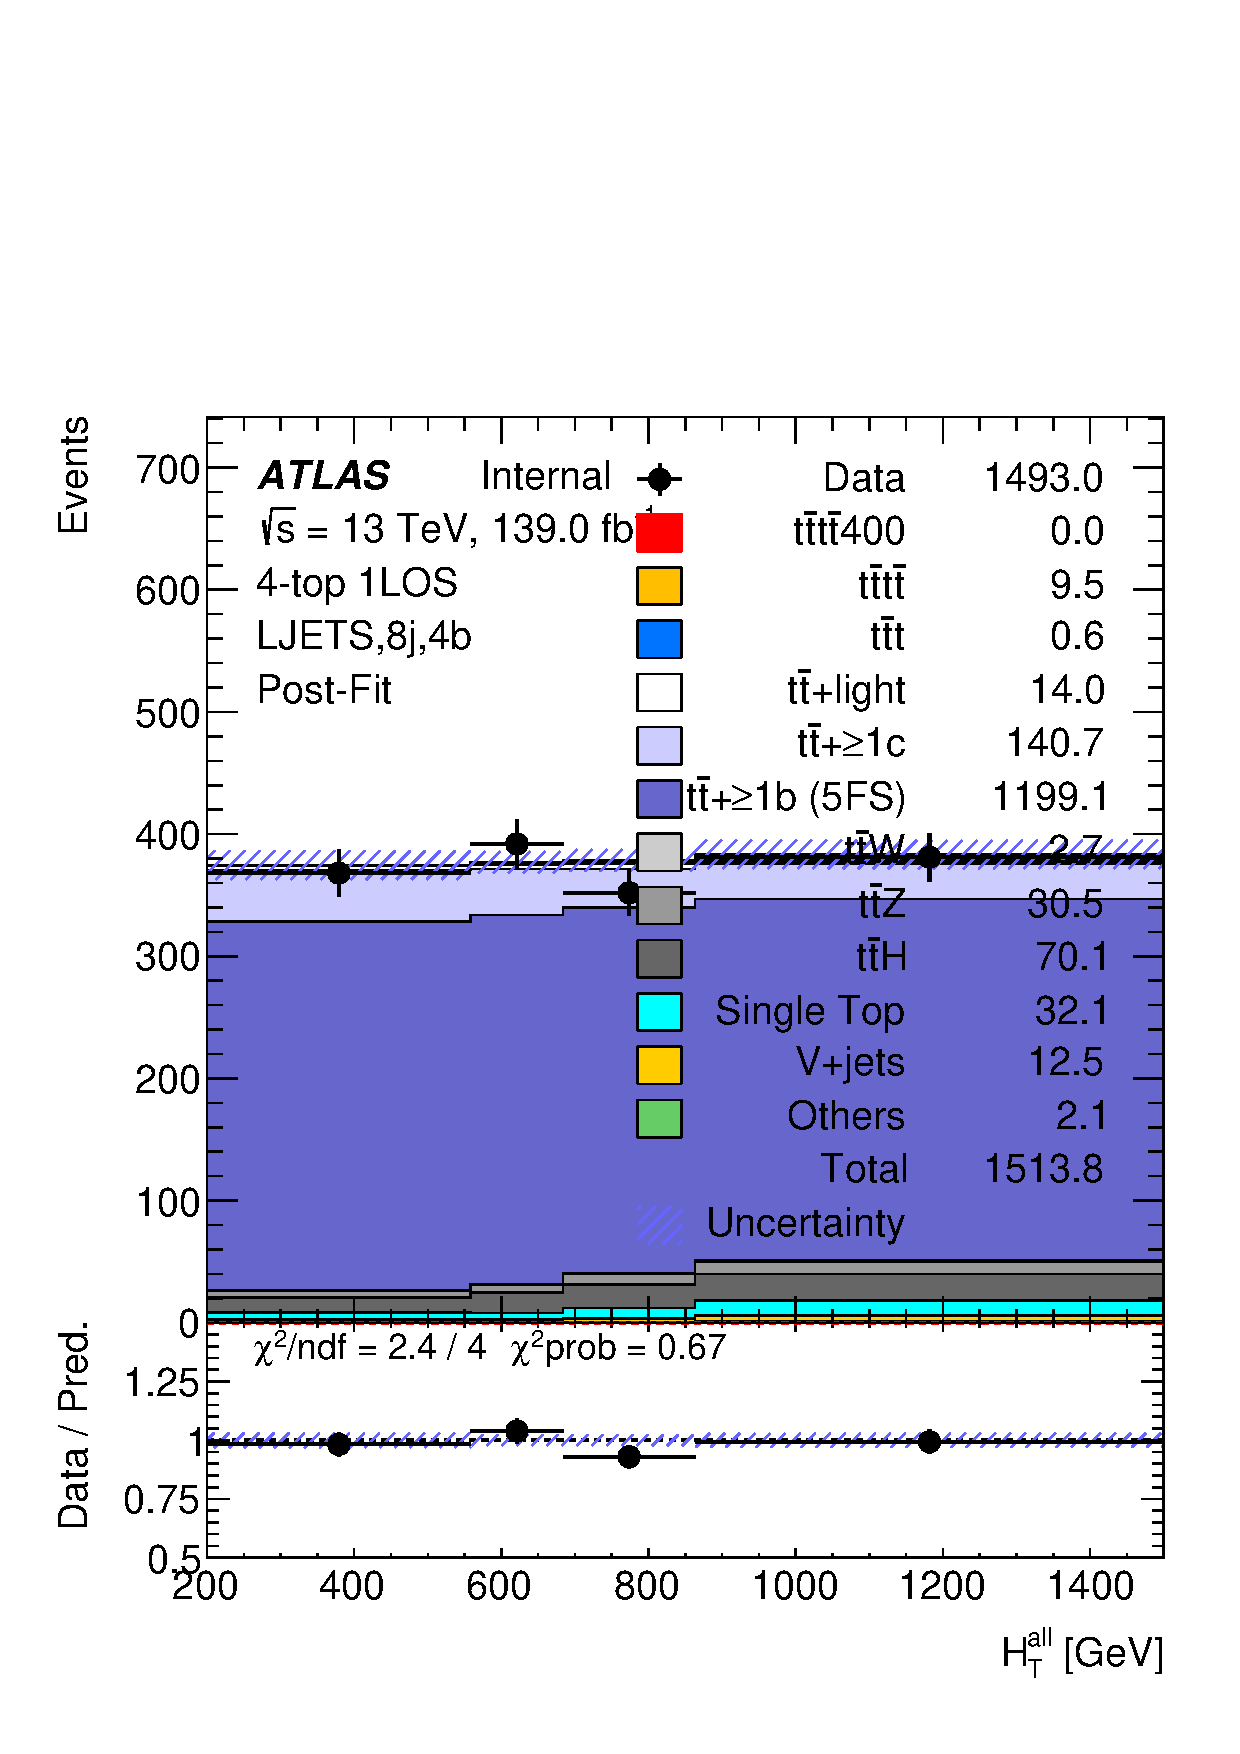
\includegraphics[width=0.23 \textwidth]{figures/fits/GNN/400/all/data_unblindedBonly/Plots/ljets_8j4b_postFit.pdf} &
        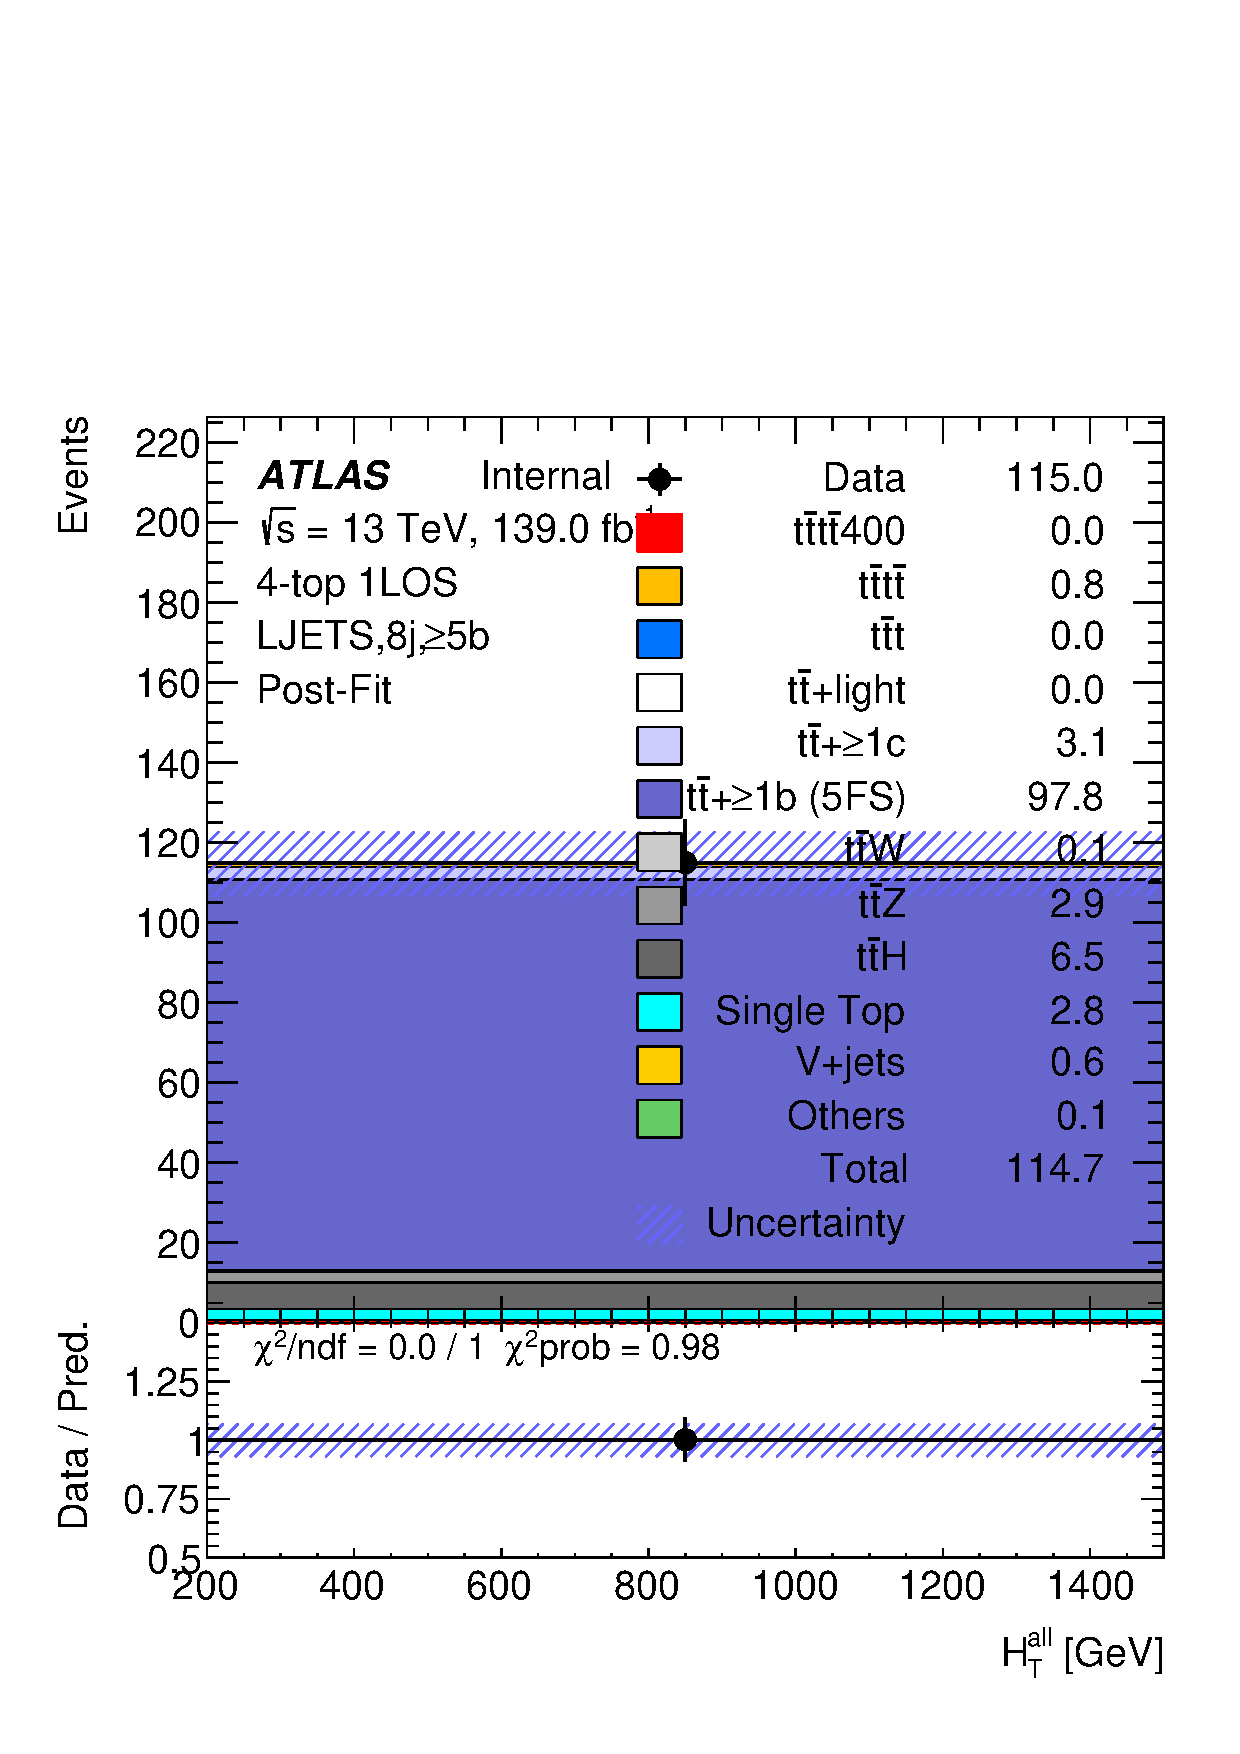
\includegraphics[width=0.23 \textwidth]{figures/fits/GNN/400/all/data_unblindedBonly/Plots/ljets_8jge5b_postFit.pdf}\\

        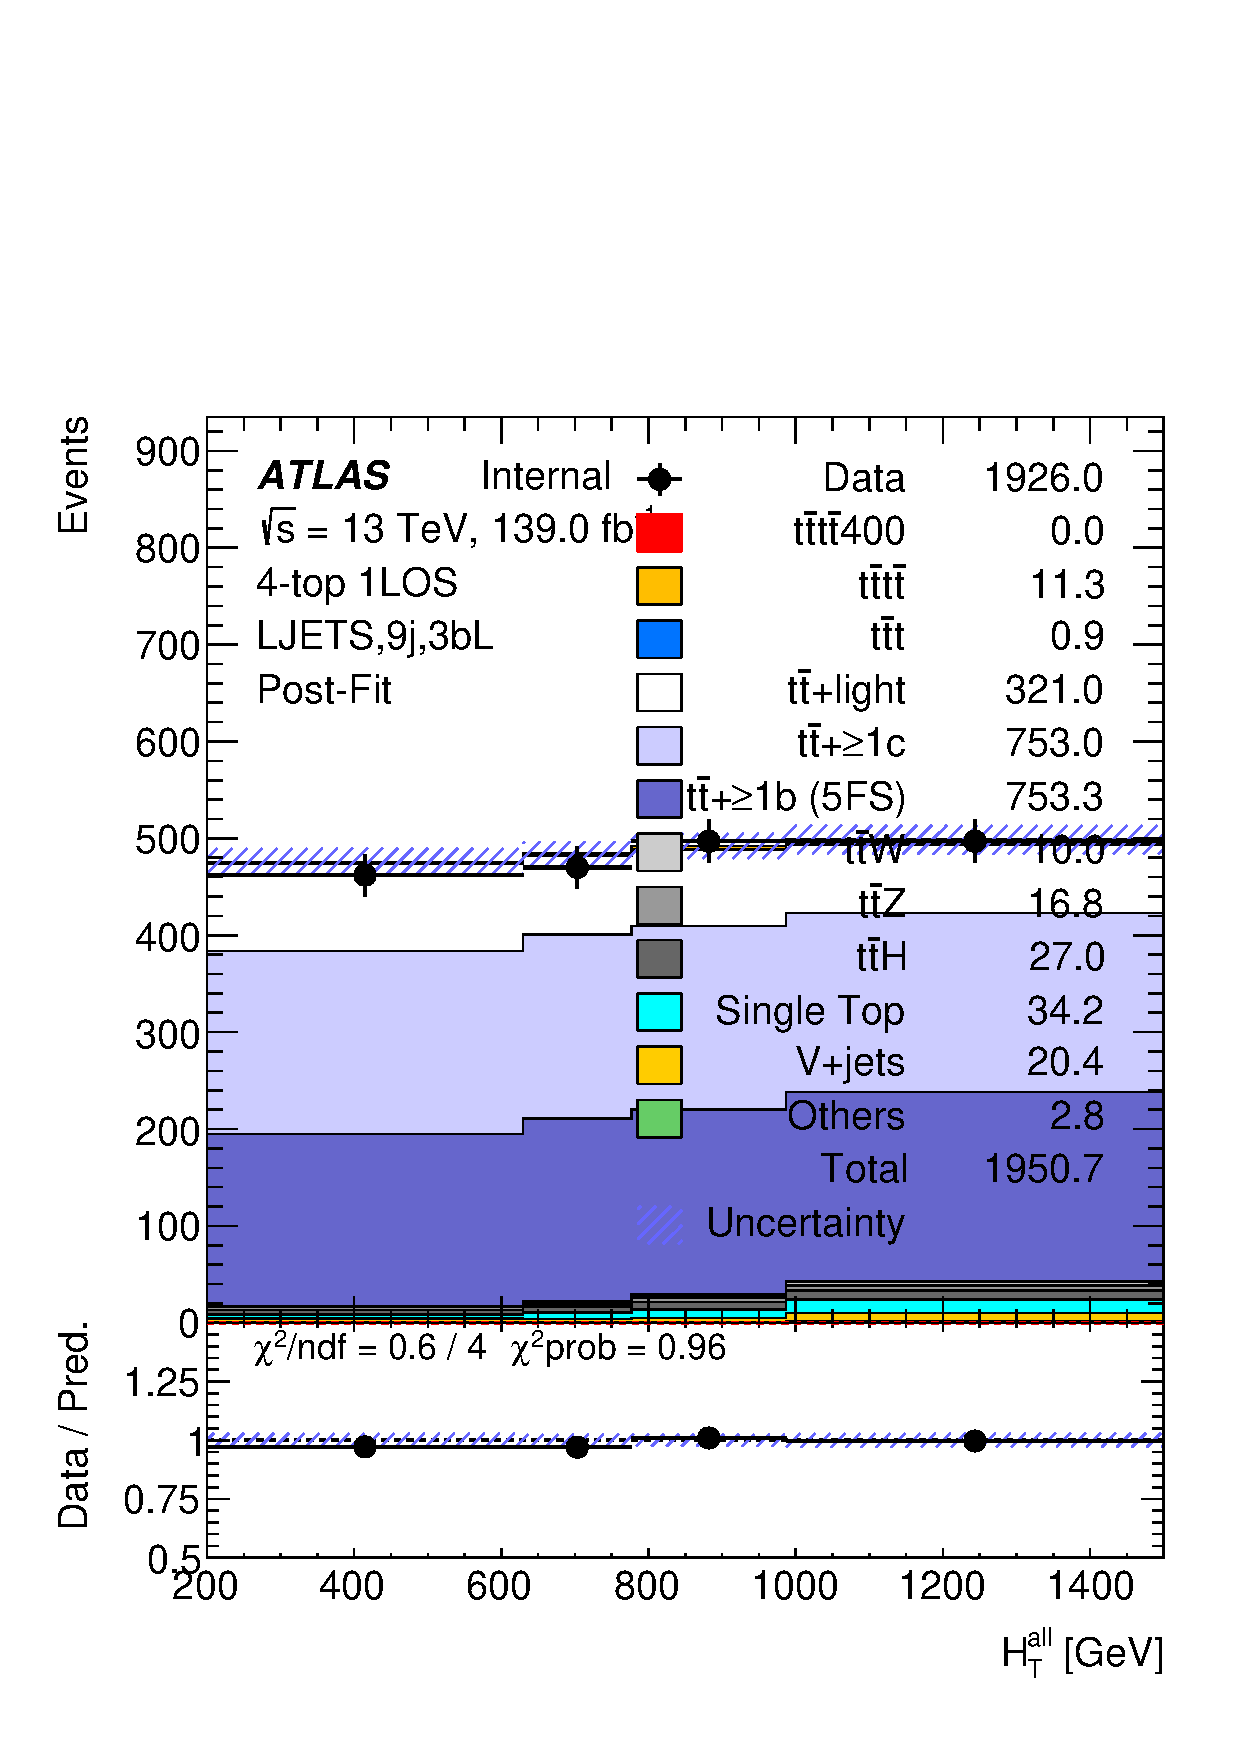
\includegraphics[width=0.23 \textwidth]{figures/fits/GNN/400/all/data_unblindedBonly/Plots/ljets_9j3bL_postFit.pdf} &
        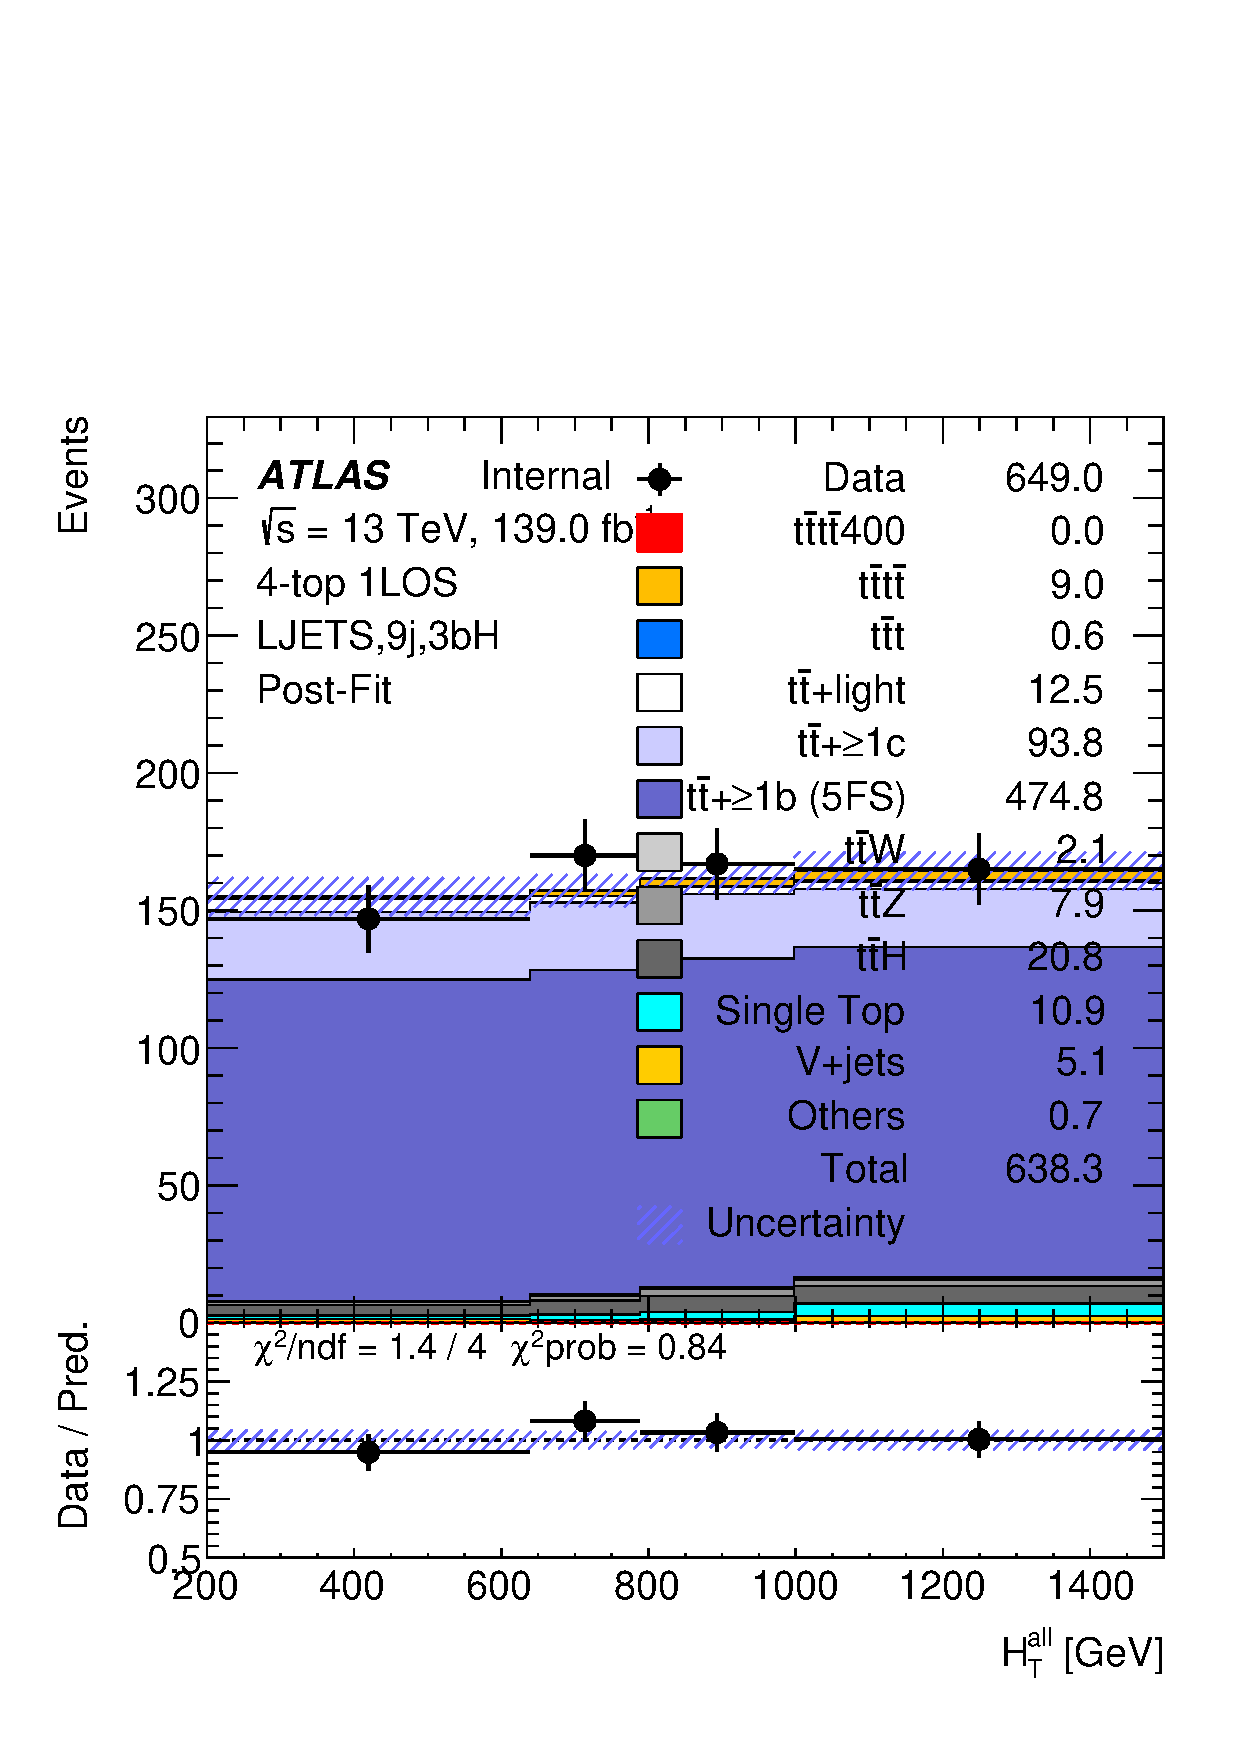
\includegraphics[width=0.23 \textwidth]{figures/fits/GNN/400/all/data_unblindedBonly/Plots/ljets_9j3bH_postFit.pdf} &
        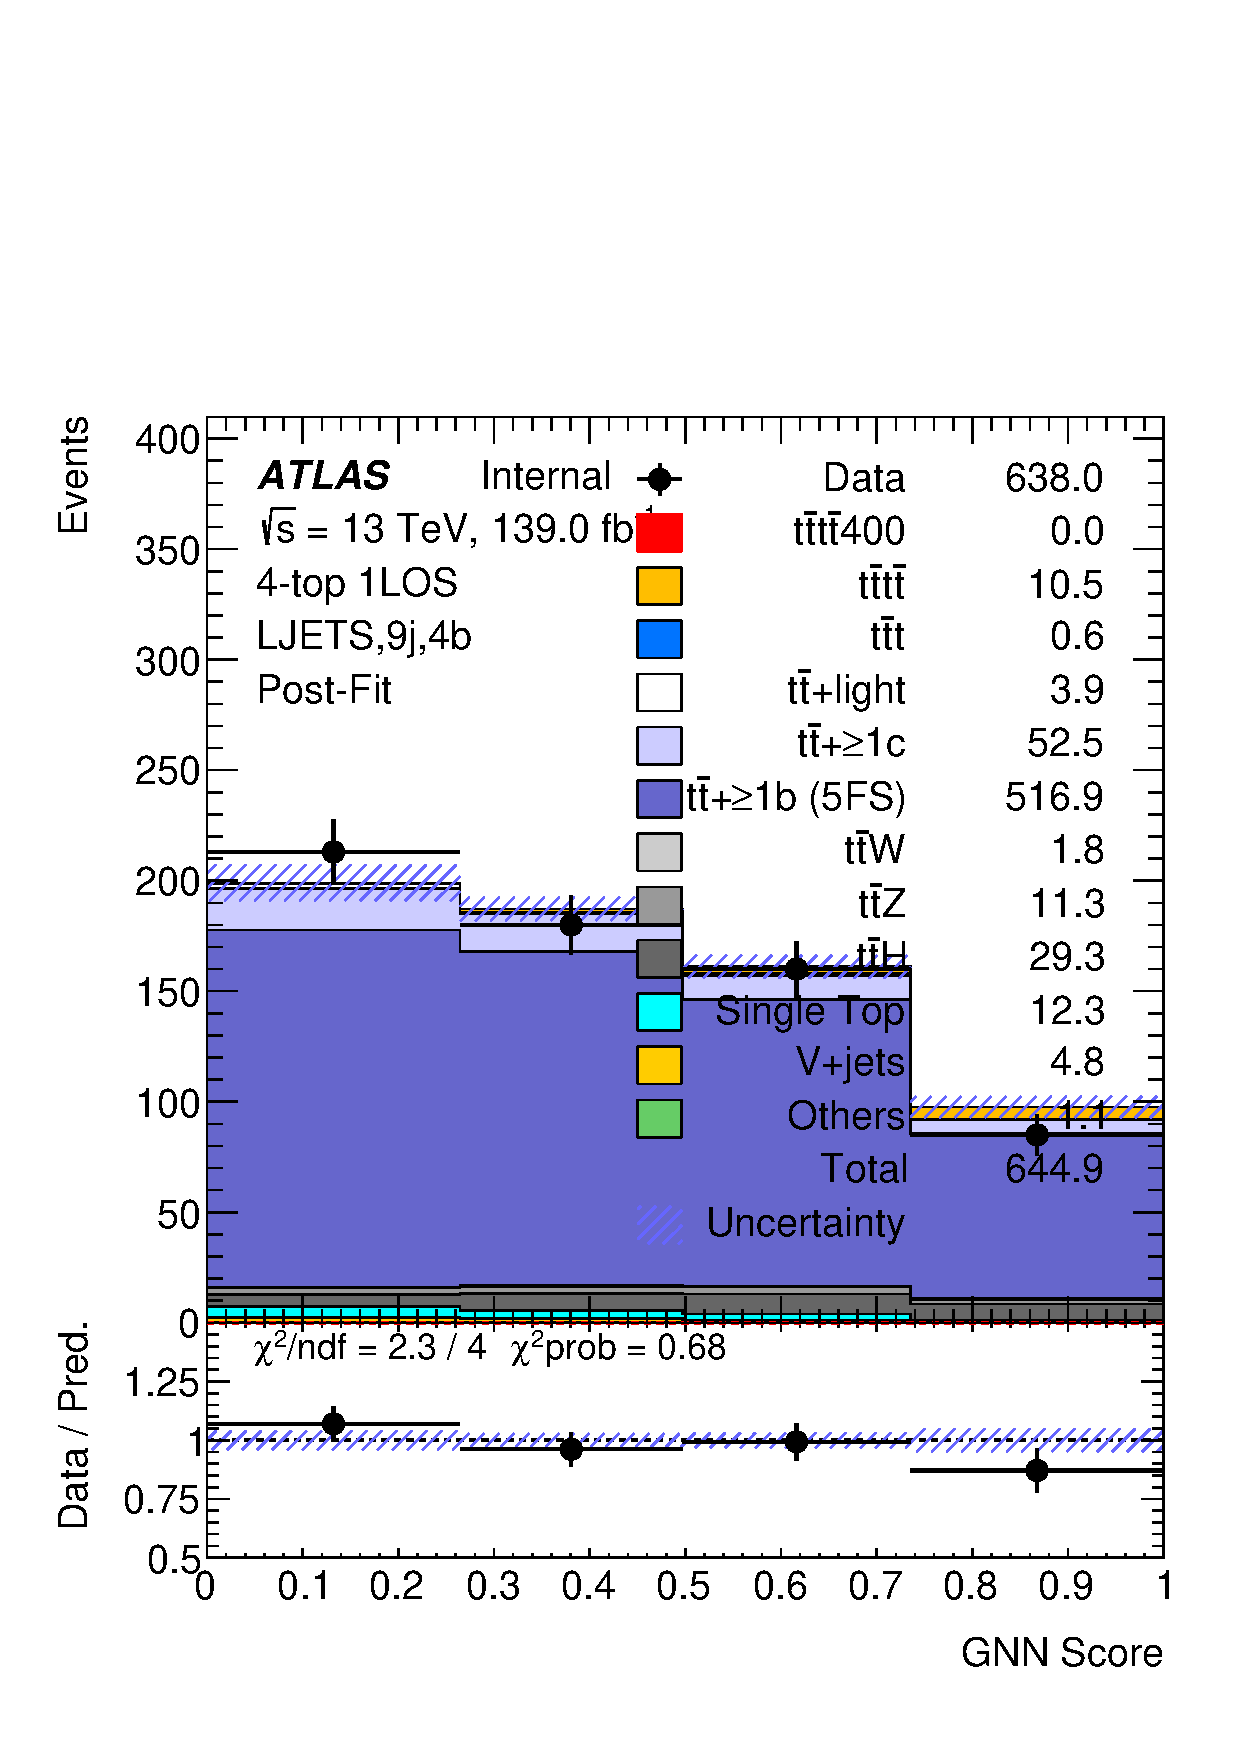
\includegraphics[width=0.23 \textwidth]{figures/fits/GNN/400/all/data_unblindedBonly/Plots/ljets_9j4b_postFit.pdf} &
        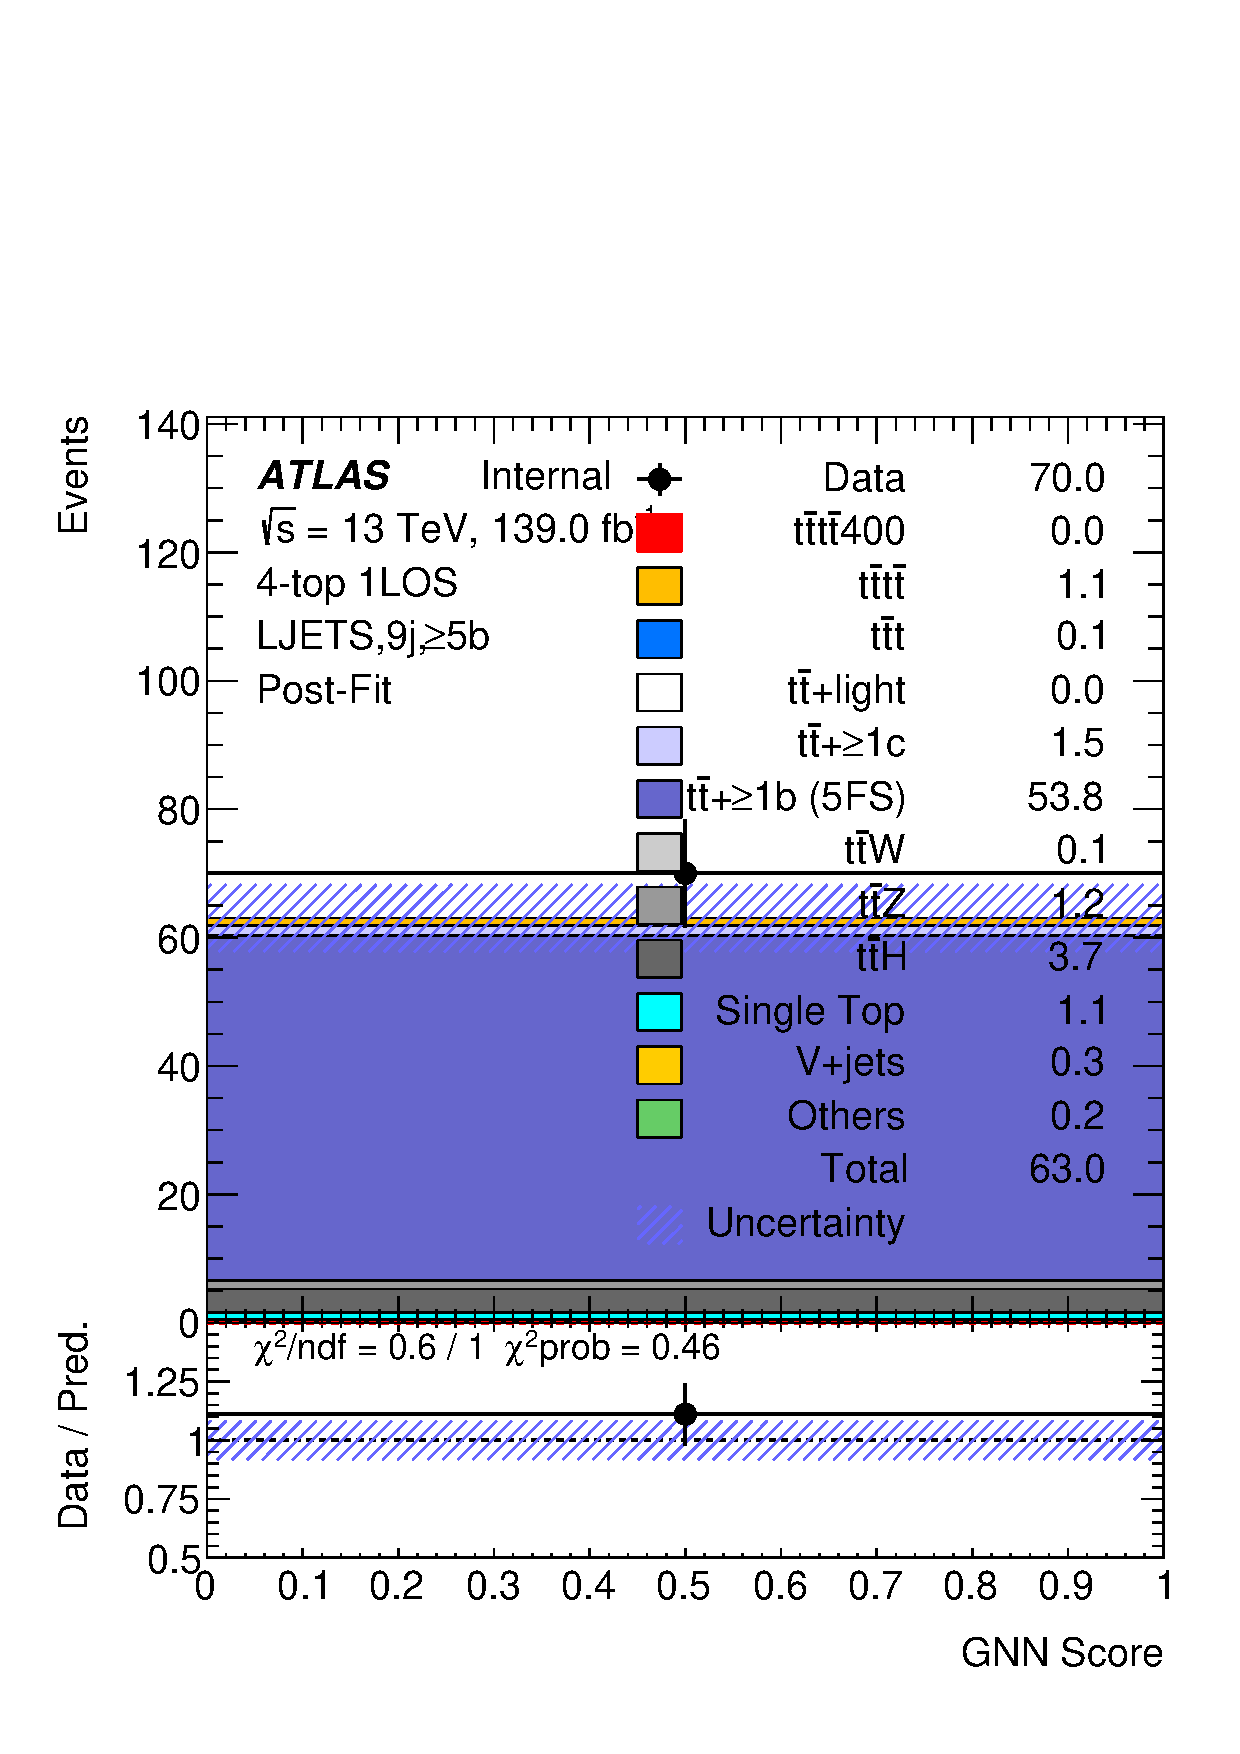
\includegraphics[width=0.23 \textwidth]{figures/fits/GNN/400/all/data_unblindedBonly/Plots/ljets_9jge5b_postFit.pdf} \\

        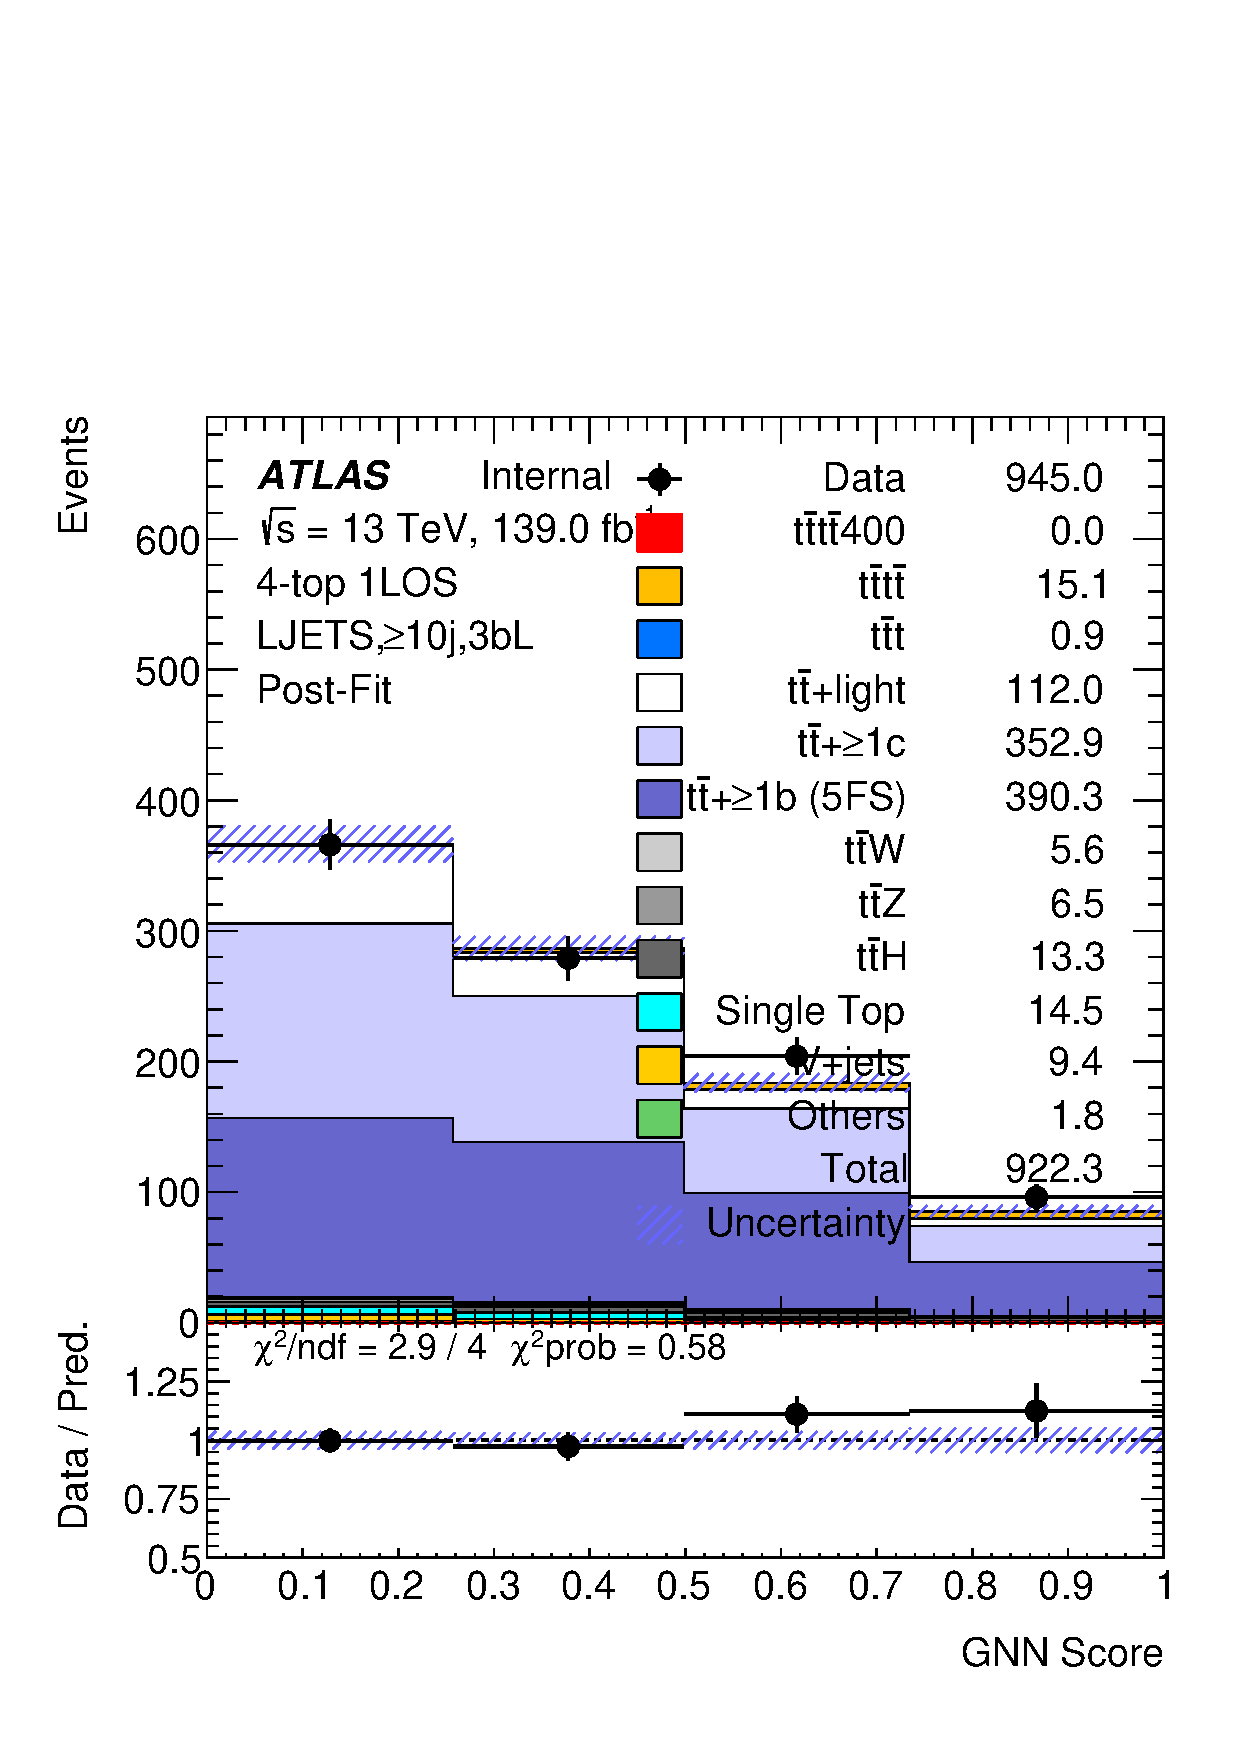
\includegraphics[width=0.23 \textwidth]{figures/fits/GNN/400/all/data_unblindedBonly/Plots/ljets_ge10j3bL_postFit.pdf} &
        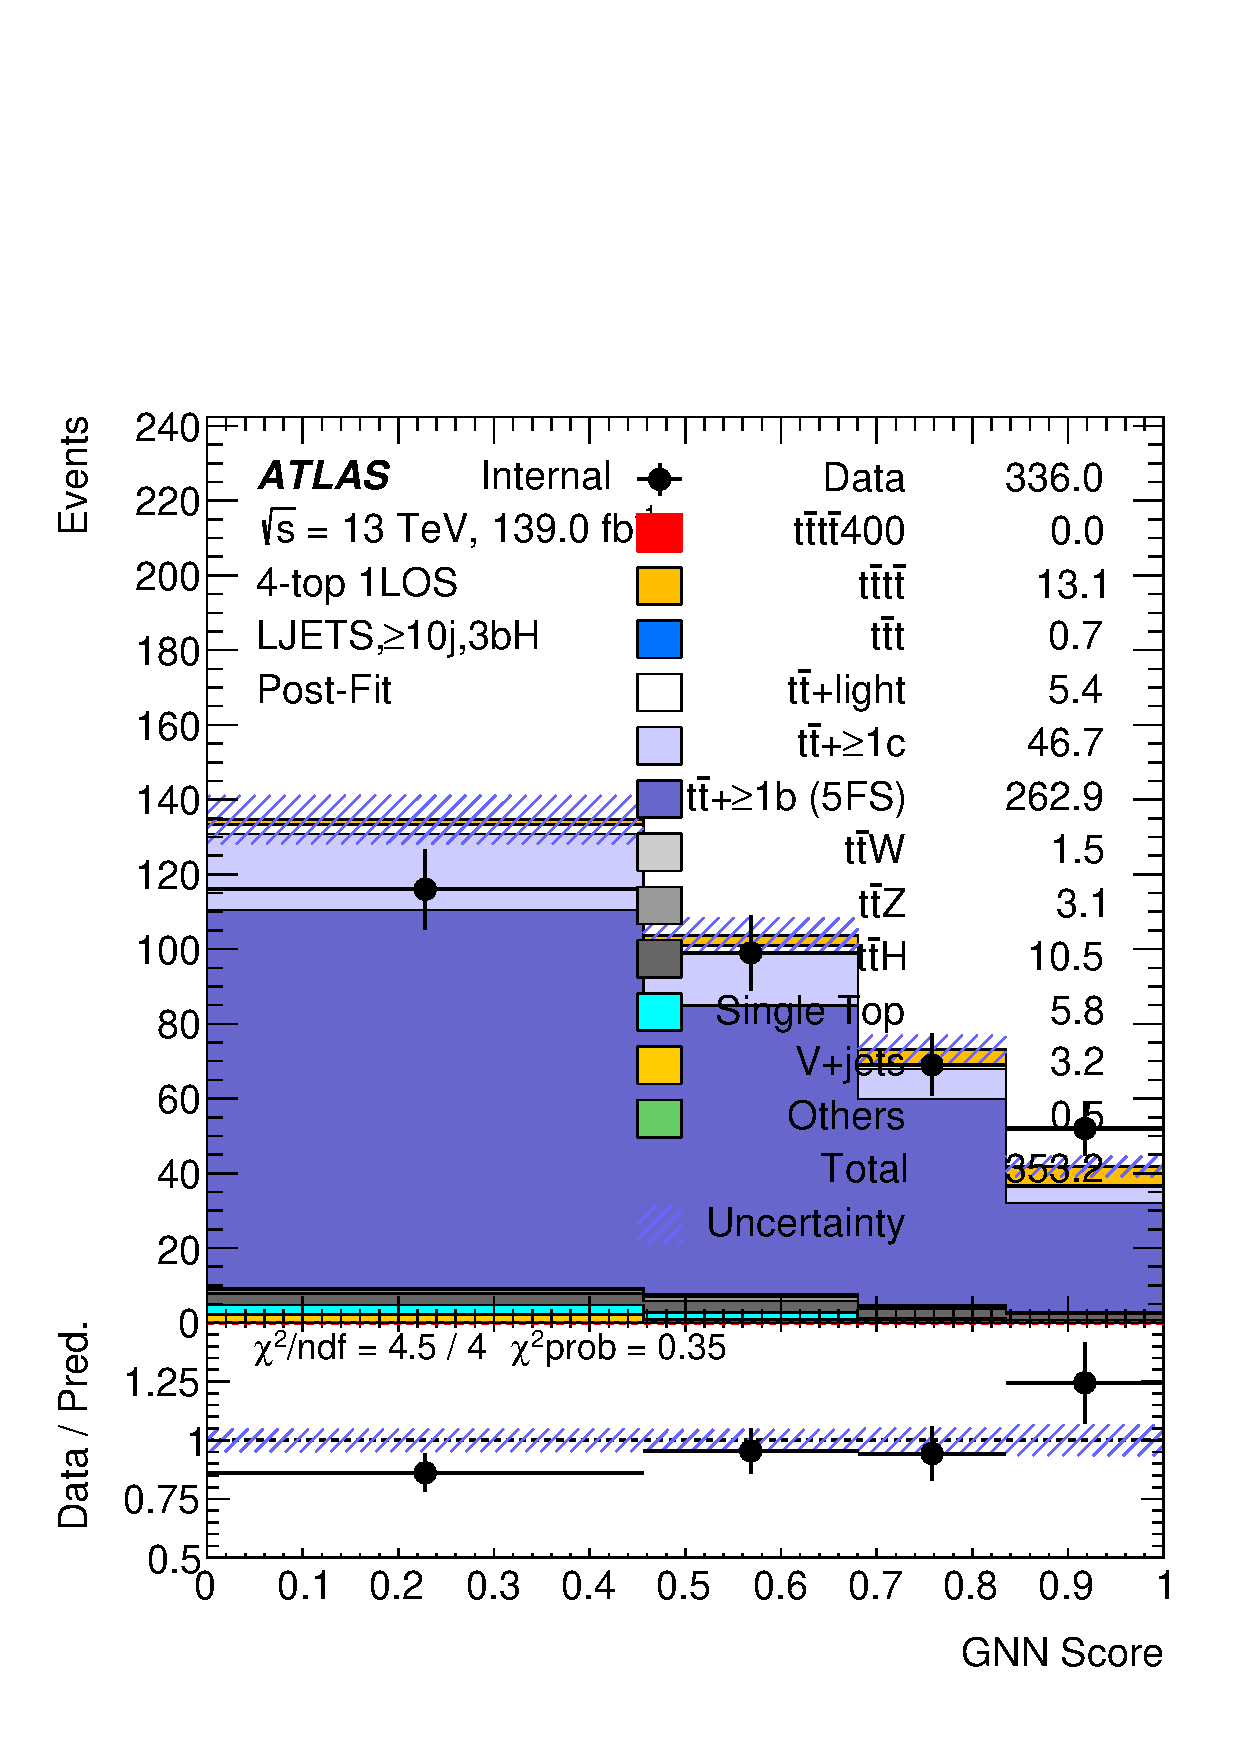
\includegraphics[width=0.23 \textwidth]{figures/fits/GNN/400/all/data_unblindedBonly/Plots/ljets_ge10j3bH_postFit.pdf} &
        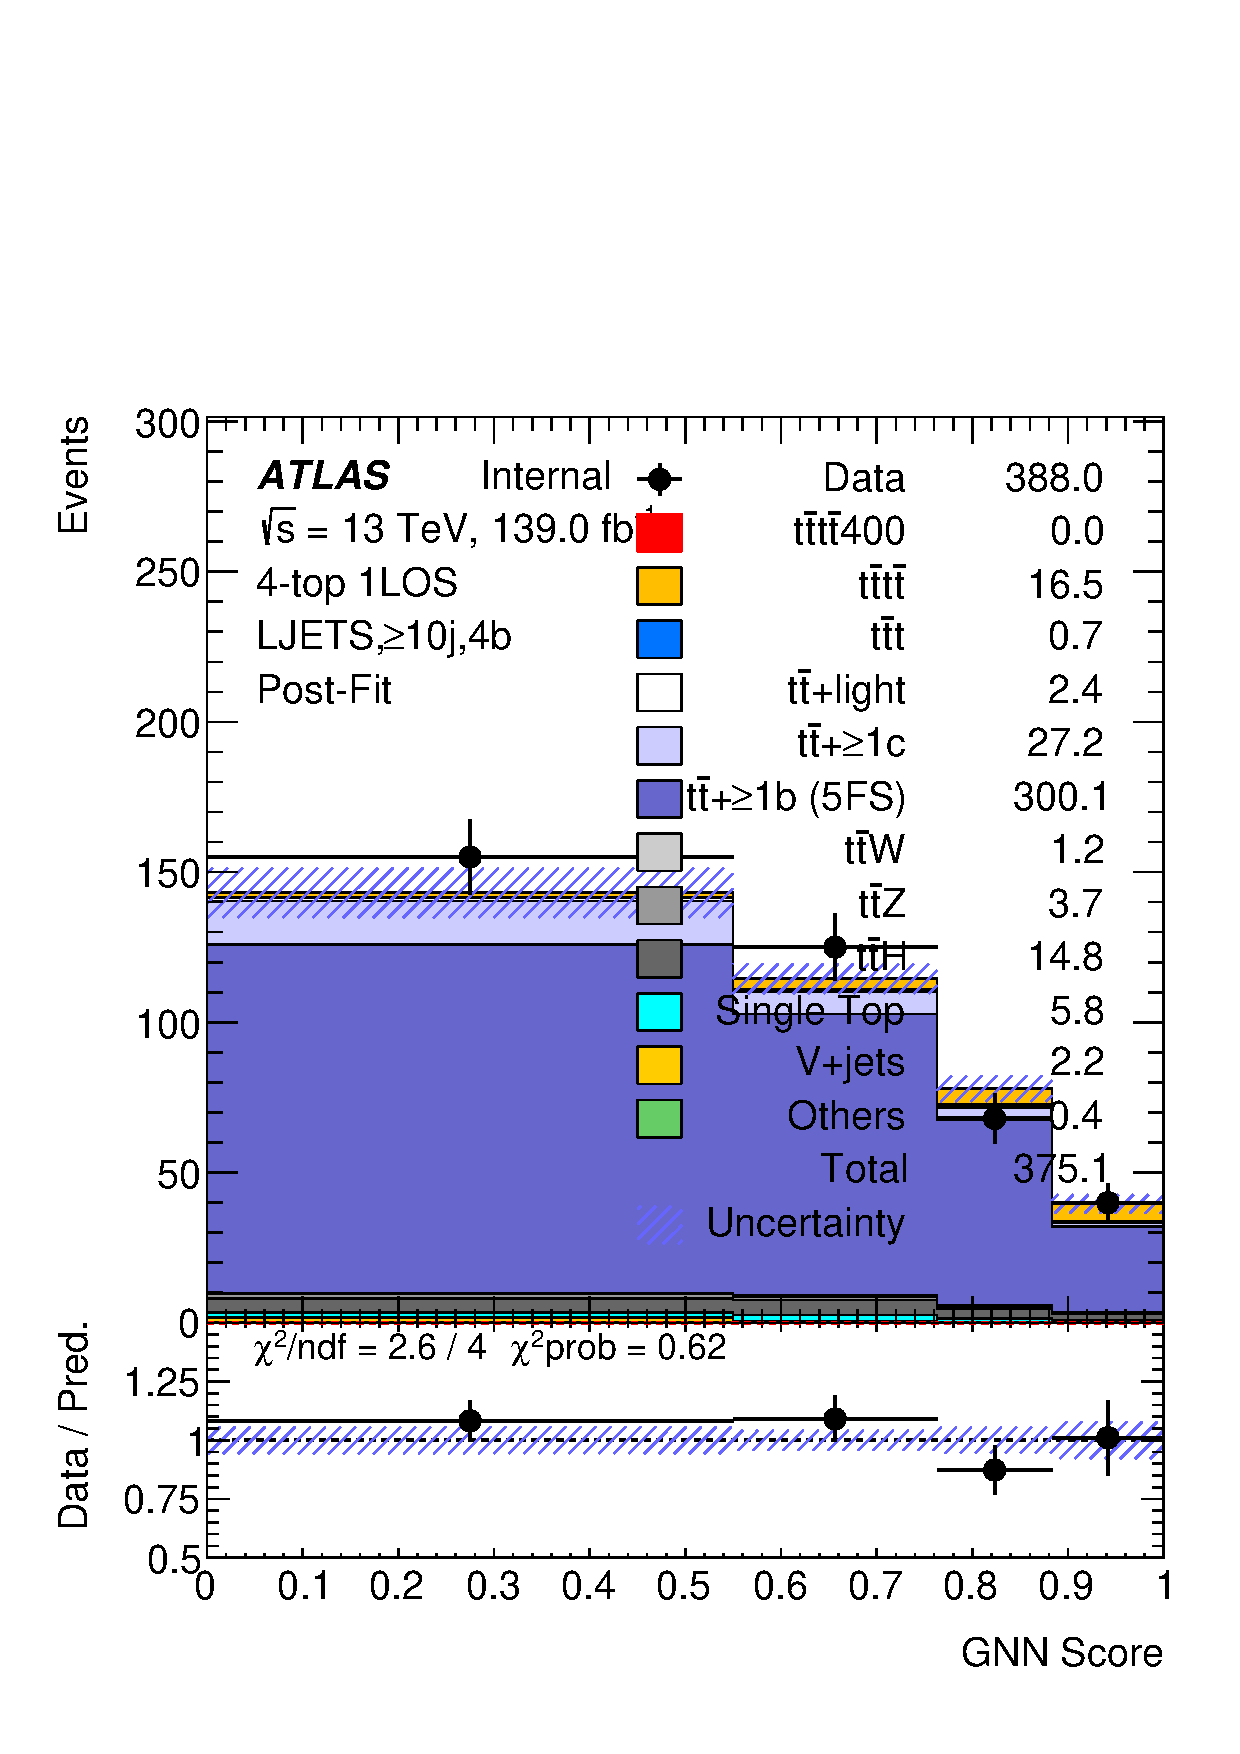
\includegraphics[width=0.23 \textwidth]{figures/fits/GNN/400/all/data_unblindedBonly/Plots/ljets_ge10j4b_postFit.pdf} &
        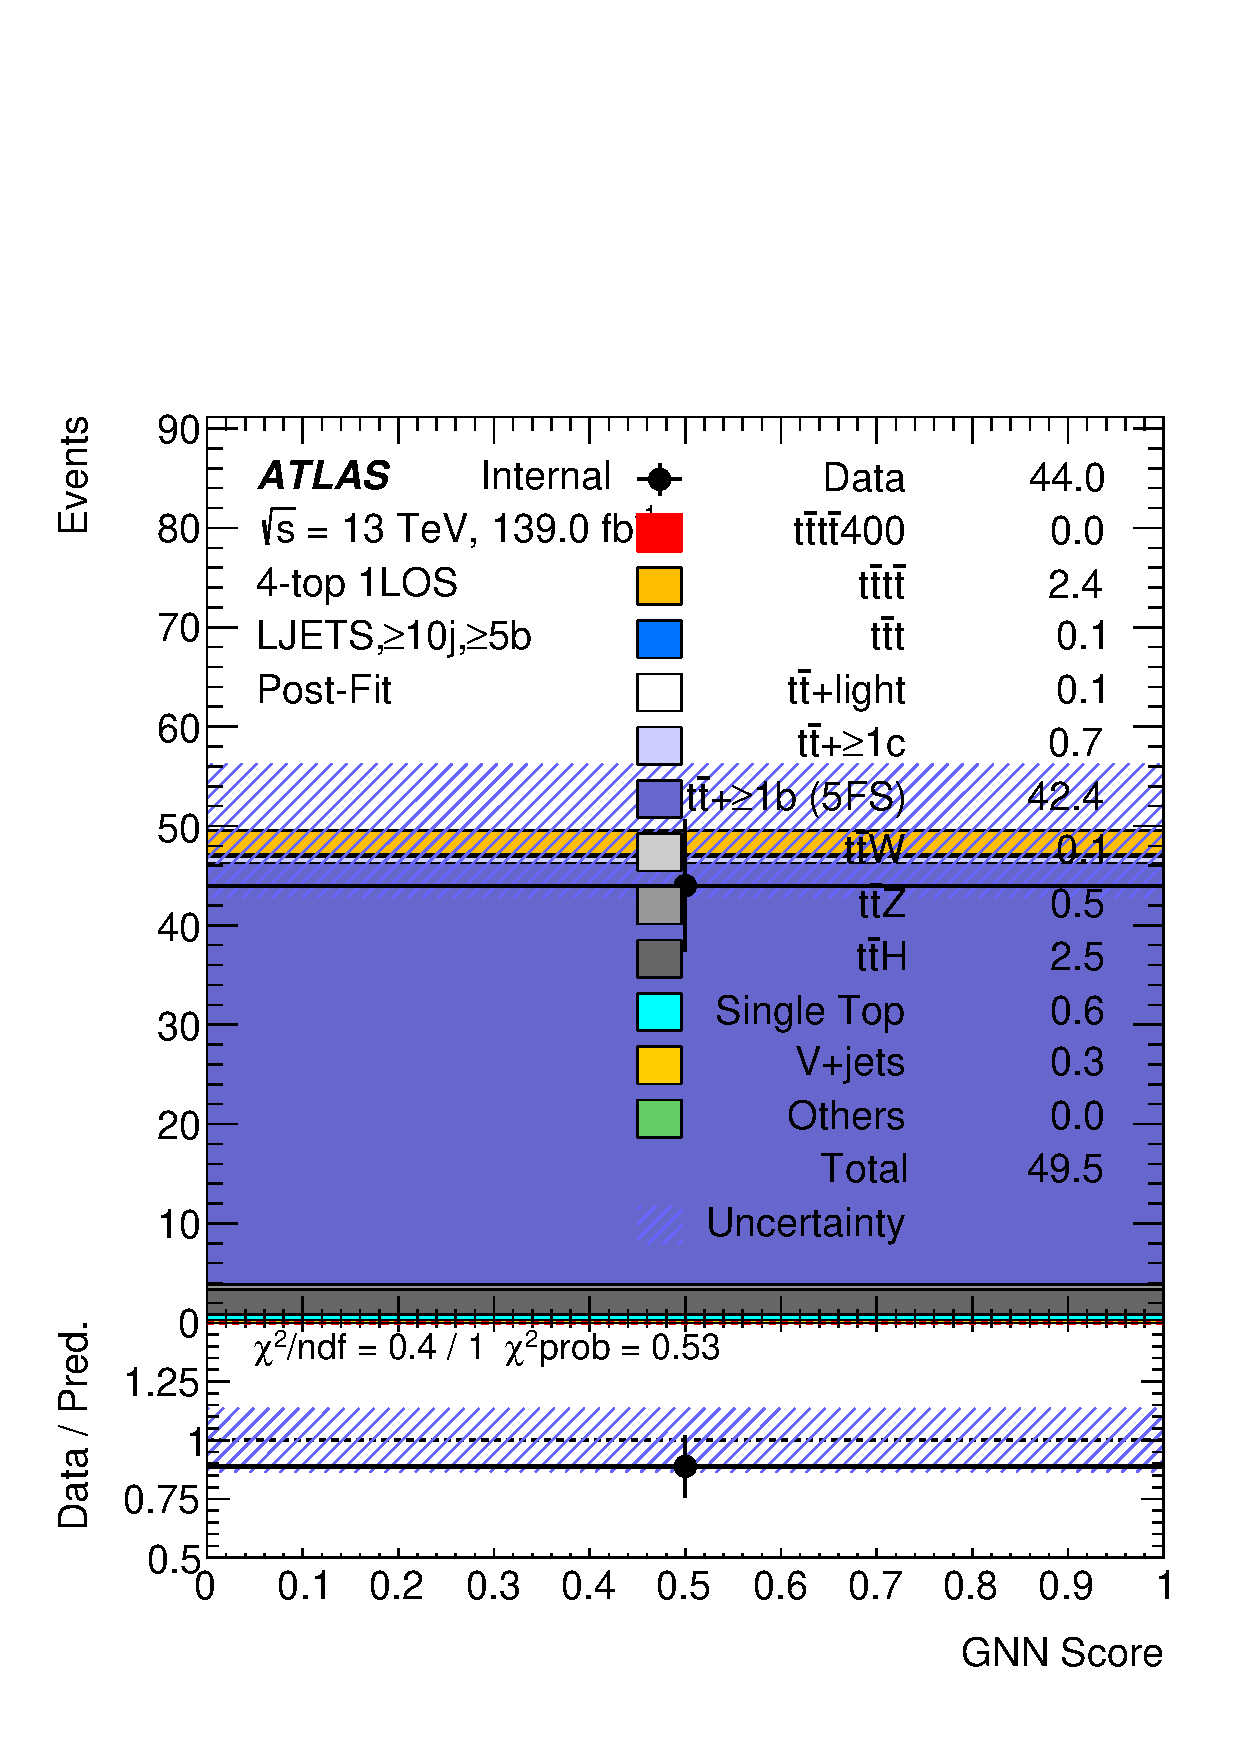
\includegraphics[width=0.23 \textwidth]{figures/fits/GNN/400/all/data_unblindedBonly/Plots/ljets_ge10jge5b_postFit.pdf} \\
        \end{tabular}
        \caption{\label{fig:unblinded_data_Bonly_postfit_1L}Post-fit distributions for 1L regions obtained with background-only unblinded data fit, compared with data yields for mH = 400 GeV. The fit is done using all regions (1L+2L).}
\end{center}
\end{figure}

\begin{figure}[htbp!]
        \begin{center} \setlength{\tabcolsep}{2.5pt}\footnotesize
        \begin{tabular}{ccc}
        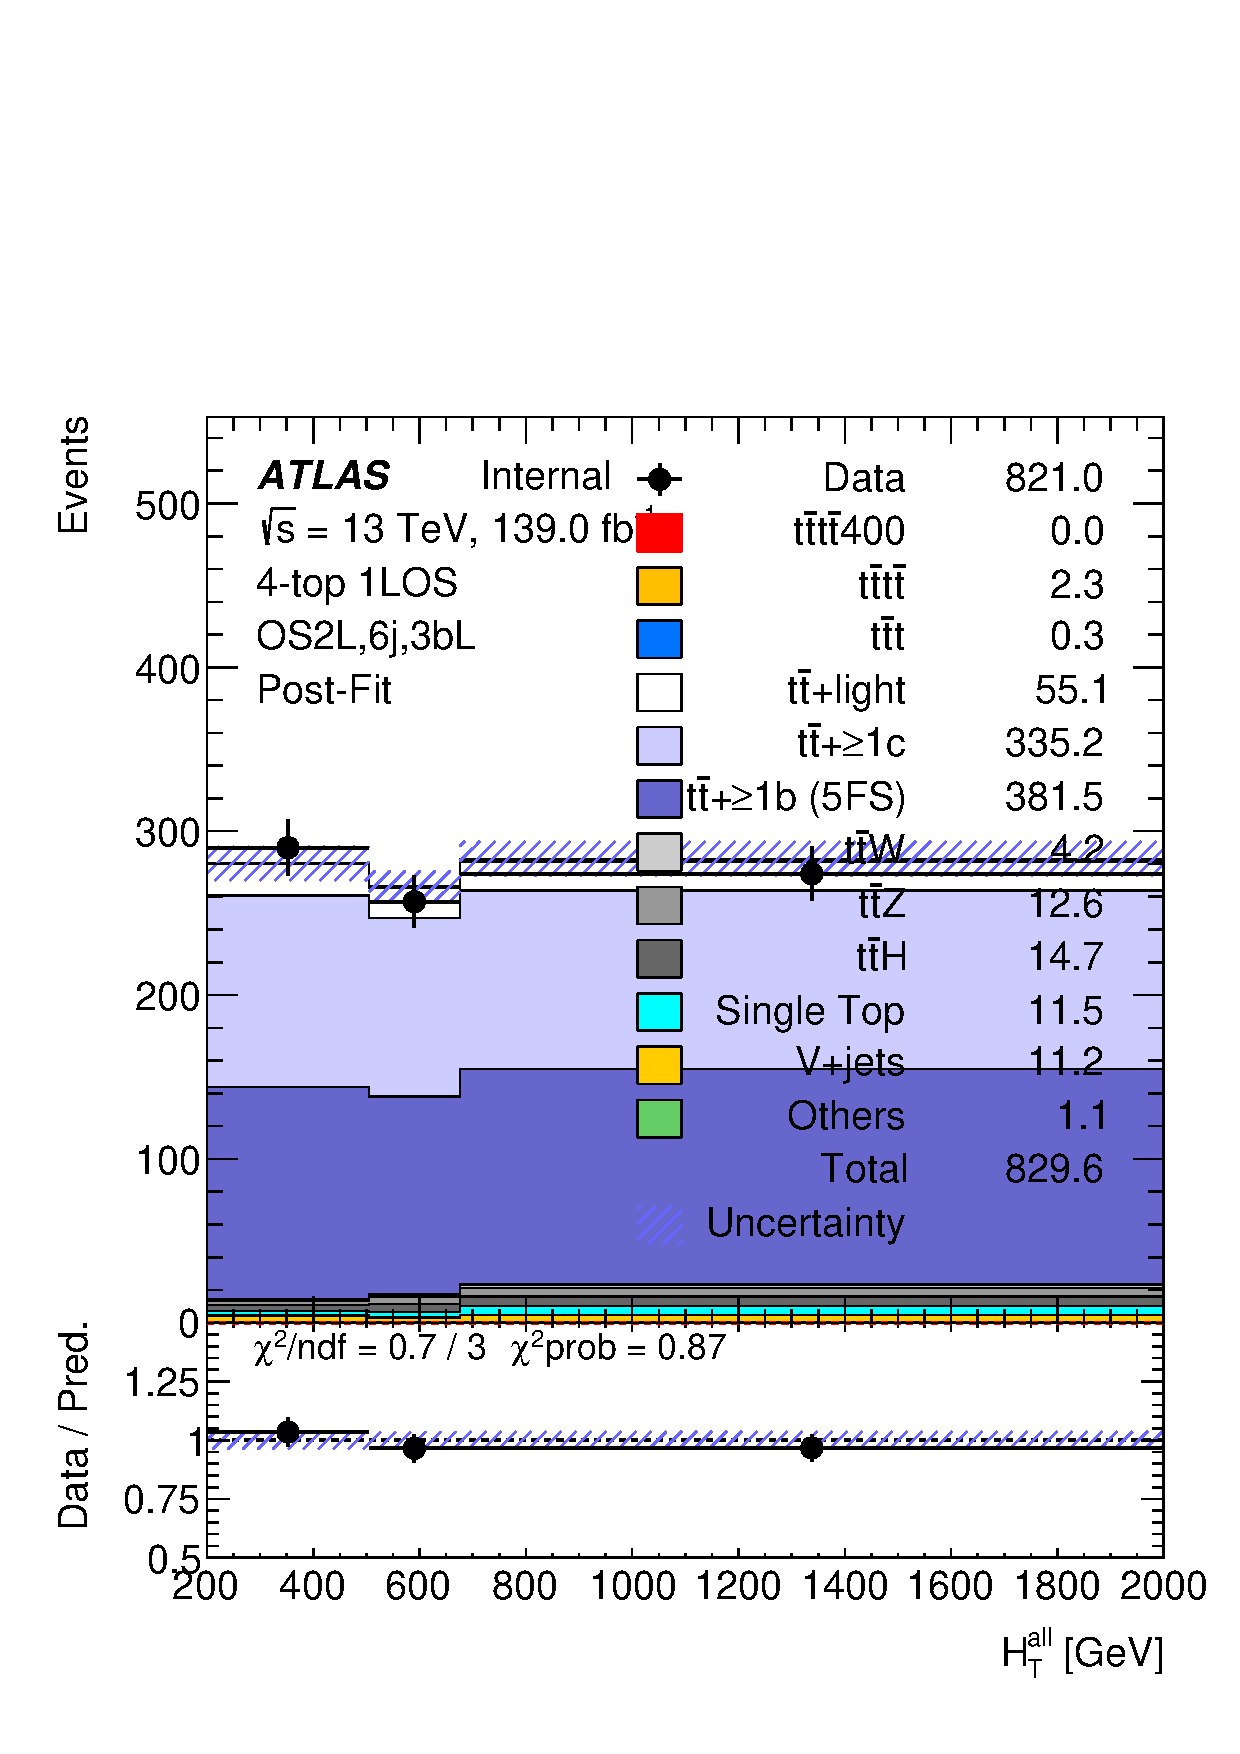
\includegraphics[width=0.31 \textwidth]{figures/fits/GNN/400/all/data_unblindedBonly/Plots/os2l_6j3bL_postFit.pdf} &
        \includegraphics[width=0.31 \textwidth]{figures/fits/GNN/400/all/data_unblindedBonly/Plots/os2l_6j3bH_postFit.pdf} &
        \includegraphics[width=0.31 \textwidth]{figures/fits/GNN/400/all/data_unblindedBonly/Plots/os2l_6jge4b_postFit.pdf} \\

        \includegraphics[width=0.31 \textwidth]{figures/fits/GNN/400/all/data_unblindedBonly/Plots/os2l_7j3bL_postFit.pdf} &
        \includegraphics[width=0.31 \textwidth]{figures/fits/GNN/400/all/data_unblindedBonly/Plots/os2l_7j3bH_postFit.pdf} &
        \includegraphics[width=0.31 \textwidth]{figures/fits/GNN/400/all/data_unblindedBonly/Plots/os2l_7jge4b_postFit.pdf} \\

        \includegraphics[width=0.31 \textwidth]{figures/fits/GNN/400/all/data_unblindedBonly/Plots/os2l_ge8j3bL_postFit.pdf} &
        \includegraphics[width=0.31 \textwidth]{figures/fits/GNN/400/all/data_unblindedBonly/Plots/os2l_ge8j3bH_postFit.pdf} &
        \includegraphics[width=0.31 \textwidth]{figures/fits/GNN/400/all/data_unblindedBonly/Plots/os2l_ge8jge4b_postFit.pdf} \\
        \end{tabular}
        \caption{\label{fig:unblinded_data_Bonly_postfit_2L}Post-fit distributions for 2LOS regions obtained with background-only unblinded data fit, compared with data yields for mH = 400 GeV. The fit is done using all regions (1L+2L)}
\end{center}
\end{figure}


\begin{figure}[htbp!]
  \centering
  \begin{subfigure}[t]{0.32\textwidth}
    \includegraphics[width=\linewidth]{figures/fits/comparisons/selections/GNN/400/data_unblindedBonly/NuisPar_comp_Instrumental.pdf}
    \subcaption{mH=400\gev}
    \label{fig:unblinded_data_Bonly_NP_mH400}
  \end{subfigure}
  \begin{subfigure}[t]{0.32\textwidth}
    \includegraphics[width=\linewidth]{figures/fits/comparisons/selections/GNN/700/data_unblindedBonly/NuisPar_comp_Instrumental.pdf}
    \subcaption{mH=700\gev}
    \label{fig:unblinded_data_Bonly_NP_mH400}
  \end{subfigure}
  \begin{subfigure}[t]{0.32\textwidth}
    \includegraphics[width=\linewidth]{figures/fits/comparisons/selections/GNN/1000/data_unblindedBonly/NuisPar_comp_Instrumental.pdf}
    \subcaption{mH=1000\gev}
    \label{fig:unblinded_data_Bonly_NP_mH400}
  \end{subfigure}
  \caption{\label{fig:unblinded_data_Bonly_NP_instrumental}Fitted pulls and constraints for the nuisance parameters corresponding to the instrumental systematic uncertainties for the background-only unblinded Data fit for three mass points. Comparison is done for three fits: using only 1L regions, using only 2LOS regions and using all regions.}
\end{figure}


\begin{figure}[htbp!]
  \centering
  \begin{subfigure}[t]{0.32\textwidth}
    \includegraphics[width=\linewidth]{figures/fits/comparisons/selections/GNN/400/data_unblindedBonly/NuisPar_comp_ttbar.pdf}
    \subcaption{mH=400\gev}
    \label{fig:unblinded_data_Bonly_NP_mH400}
  \end{subfigure}
  \begin{subfigure}[t]{0.32\textwidth}
    \includegraphics[width=\linewidth]{figures/fits/comparisons/selections/GNN/700/data_unblindedBonly/NuisPar_comp_ttbar.pdf}
    \subcaption{mH=700\gev}
    \label{fig:unblinded_data_Bonly_NP_mH400}
  \end{subfigure}
  \begin{subfigure}[t]{0.32\textwidth}
    \includegraphics[width=\linewidth]{figures/fits/comparisons/selections/GNN/1000/data_unblindedBonly/NuisPar_comp_ttbar.pdf}
    \subcaption{mH=1000\gev}
    \label{fig:unblinded_data_Bonly_NP_mH400}
  \end{subfigure}
  \caption{\label{fig:unblinded_data_Bonly_NP_ttbar}Fitted pulls and constraints for the nuisance parameters corresponding to the \ttbar systematic uncertainties for the background-only unblinded Data fit for three mass points. Comparison is done for three fits: using only 1L regions, using only 2LOS regions and using all regions.}
\end{figure}


\begin{figure}[htbp!]
  \centering
  \begin{subfigure}[t]{0.32\textwidth}
    \includegraphics[width=\linewidth]{figures/fits/comparisons/selections/GNN/400/data_unblindedBonly/NuisPar_comp_Other.pdf}
    \subcaption{mH=400\gev}
    \label{fig:unblinded_data_Bonly_NP_mH400}
  \end{subfigure}
  \begin{subfigure}[t]{0.32\textwidth}
    \includegraphics[width=\linewidth]{figures/fits/comparisons/selections/GNN/700/data_unblindedBonly/NuisPar_comp_Other.pdf}
    \subcaption{mH=700\gev}
    \label{fig:unblinded_data_Bonly_NP_mH400}
  \end{subfigure}
  \begin{subfigure}[t]{0.32\textwidth}
    \includegraphics[width=\linewidth]{figures/fits/comparisons/selections/GNN/1000/data_unblindedBonly/NuisPar_comp_Other.pdf}
    \subcaption{mH=1000\gev}
    \label{fig:unblinded_data_Bonly_NP_mH400}
  \end{subfigure}
  \caption{\label{fig:unblinded_data_Bonly_NP_other}Fitted pulls and constraints for the  nuisance parameters corresponding to the non-\ttbar-background systematic uncertainties for the background-only unblinded Data fit for three mass points. Comparison is done for three fits: using only 1L regions, using only 2LOS regions and using all regions.}
\end{figure}



\begin{figure}[htbp!]
  \centering
  \begin{subfigure}[t]{0.32\textwidth}
    \includegraphics[width=\linewidth]{figures/fits/comparisons/massPoints/GNN/1L/data_unblindedBonly/NuisPar_comp_Instrumental.pdf}
    \subcaption{1L}
    \label{fig:unblinded_data_Bonly_NP_1L_instrumental}
  \end{subfigure}
  \begin{subfigure}[t]{0.32\textwidth}
    \includegraphics[width=\linewidth]{figures/fits/comparisons/massPoints/GNN/2L/data_unblindedBonly/NuisPar_comp_Instrumental.pdf}
    \subcaption{2L}
    \label{fig:unblinded_data_Bonly_NP_2L_instrumental}
  \end{subfigure}
  \begin{subfigure}[t]{0.32\textwidth}
    \includegraphics[width=\linewidth]{figures/fits/comparisons/massPoints/GNN/all/data_unblindedBonly/NuisPar_comp_Instrumental.pdf}
    \subcaption{1L+2L}
    \label{fig:unblinded_data_Bonly_NP_all_instrumental}
  \end{subfigure}
  \caption{Fitted pulls and constraints for the nuisance parameters corresponding to the instrumental systematic uncertainties for the background-only unblinded Data fit for three types of fits: using only 1L regions, using only 2L regions, and using all regions. Comparison is done for five mass points.}
\label{fig:unblinded_data_Bonly_NP_mass_instrumental}
\end{figure}


\begin{figure}[htbp!]
  \centering
  \begin{subfigure}[t]{0.32\textwidth}
    \includegraphics[width=\linewidth]{figures/fits/comparisons/massPoints/GNN/1L/data_unblindedBonly/NuisPar_comp_ttbar.pdf}
    \subcaption{1L}
    \label{fig:unblinded_data_Bonly_NP_1L}
  \end{subfigure}
  \begin{subfigure}[t]{0.32\textwidth}
    \includegraphics[width=\linewidth]{figures/fits/comparisons/massPoints/GNN/2L/data_unblindedBonly/NuisPar_comp_ttbar.pdf}
    \subcaption{2L}
    \label{fig:unblinded_data_Bonly_NP_2L}
  \end{subfigure}
  \begin{subfigure}[t]{0.32\textwidth}
    \includegraphics[width=\linewidth]{figures/fits/comparisons/massPoints/GNN/all/data_unblindedBonly/NuisPar_comp_ttbar.pdf}
    \subcaption{1L+2L}
    \label{fig:unblinded_data_Bonly_NP_all}
  \end{subfigure}
  \caption{Fitted pulls and constraints for the nuisance parameters corresponding to the \ttbar systematic uncertainties for the background-only unblinded Data fit for three types of fits: using only 1L regions, using only 2L regions, and using all regions. Comparison is done for five mass points.}
\label{fig:unblinded_data_Bonly_NP_mass_ttbar}
\end{figure}


\begin{figure}[htbp!]
  \centering
  \begin{subfigure}[t]{0.32\textwidth}
    \includegraphics[width=\linewidth]{figures/fits/comparisons/massPoints/GNN/1L/data_unblindedBonly/NuisPar_comp_Other.pdf}
    \subcaption{1L}
    \label{fig:unblinded_data_Bonly_NP_1L_other}
  \end{subfigure}
  \begin{subfigure}[t]{0.32\textwidth}
    \includegraphics[width=\linewidth]{figures/fits/comparisons/massPoints/GNN/2L/data_unblindedBonly/NuisPar_comp_Other.pdf}
    \subcaption{2L}
    \label{fig:unblinded_data_Bonly_NP_2L_other}
  \end{subfigure}
  \begin{subfigure}[t]{0.32\textwidth}
    \includegraphics[width=\linewidth]{figures/fits/comparisons/massPoints/GNN/all/data_unblindedBonly/NuisPar_comp_Other.pdf}
    \subcaption{1L+2L}
    \label{fig:unblinded_data_Bonly_NP_all_other}
  \end{subfigure}
  \caption{Fitted pulls and constraints for the nuisance parameters corresponding to the non-\ttbar-background systematic uncertainties for the background-only unblinded Data fit for three types of fits: using only 1L regions, using only 2L regions, and using all regions. Comparison is done for five mass points.}
\label{fig:unblinded_data_Bonly_NP_mass_other}
\end{figure}


\begin{figure}[htbp!]
        \centering
        \includegraphics[width=\linewidth]{figures/fits/GNN/400/1L/data_unblindedBonly/CorrMatrix.pdf}
        \caption{\label{fig:unblinded_data_Bonly_corr_mH400_Data_1L}Correlation matrix for the 1L unblinded data fit for mH = 400 GeV}
\end{figure}

\begin{figure}[htbp!]
        \centering
        \includegraphics[width=\linewidth]{figures/fits/GNN/400/2L/data_unblindedBonly/CorrMatrix.pdf}
        \caption{\label{fig:unblinded_data_Bonly_corr_mH400_Data_2L}Correlation matrix for the 2LOS unblinded data fit for mH = 400 GeV}
\end{figure}

\begin{figure}[htbp!]
        \centering
        \includegraphics[width=\linewidth]{figures/fits/GNN/400/all/data_unblindedBonly/CorrMatrix.pdf}
        \caption{\label{fig:unblinded_data_Bonly_corr_mH400_Data_all}Correlation matrix for the 1L/2LOS combined unblinded data fit for mH = 400 GeV}
\end{figure}




\begin{figure}[htbp!]
  \centering
  \includegraphics[width=0.4 \textwidth]{figures/fits/significanceVsMass.pdf}
  \caption{\label{fig:data_Bonly_significance}Comparison of the observed significance.}
\end{figure}



%-------------------------------------------------------------------------------

%-------------------------------------------------------------------------------
\FloatBarrier
\section{Fits to unblinded data - signal+background}% Peter
\label{sec:unblinded_SplusB}
A fit using data is performed on using all bins, without blinding. The signal sample is also included in the fit (it is a signal+background fit). The unblinded data fit is performed over all control and signal regions (combined 1L+2LOS), and with all available samples and systematics. The dominant \ttbar background is reweighted using the NN method.

The post-fit distributions associated with each background and signal region are shown in Figure \ref{fig:unblinded_data_SplusB_postfit_1L} for 1L regions and Figure \ref{fig:unblinded_data_SplusB_postfit_2L} for 2LOS regions from the combined fit using mass point $m_H=400$ GeV. The nuisance parameter pulls and constraints are compared between 1L, 2LOS, and the combined fit in Figures \ref{fig:unblinded_data_SplusB_NP_instrumental}, \ref{fig:unblinded_data_SplusB_NP_ttbar}, and \ref{fig:unblinded_data_SplusB_NP_other}. Comparison for the fits using GNN outputs trained on various mass points are shown in Figures \ref{fig:unblinded_data_SplusB_NP_mass_instrumental}, \ref{fig:unblinded_data_SplusB_NP_mass_ttbar}, and \ref{fig:unblinded_data_SplusB_NP_mass_other}. Correlation matrices for systematics for the fit are shown in Figure Figure \ref{fig:unblinded_data_SplusB_corr_mH400_Data_all}.

\begin{figure}[htbp!]
        \begin{center} \setlength{\tabcolsep}{2.5pt}\footnotesize
        \begin{tabular}{cccc}
        \includegraphics[width=0.23 \textwidth]{figures/fits/GNN/400/all/data_unblindedSplusB/Plots/ljets_8j3bL_postFit.pdf} &
        \includegraphics[width=0.23 \textwidth]{figures/fits/GNN/400/all/data_unblindedSplusB/Plots/ljets_8j3bH_postFit.pdf} &
        \includegraphics[width=0.23 \textwidth]{figures/fits/GNN/400/all/data_unblindedSplusB/Plots/ljets_8j4b_postFit.pdf} &
        \includegraphics[width=0.23 \textwidth]{figures/fits/GNN/400/all/data_unblindedSplusB/Plots/ljets_8jge5b_postFit.pdf}\\

        \includegraphics[width=0.23 \textwidth]{figures/fits/GNN/400/all/data_unblindedSplusB/Plots/ljets_9j3bL_postFit.pdf} &
        \includegraphics[width=0.23 \textwidth]{figures/fits/GNN/400/all/data_unblindedSplusB/Plots/ljets_9j3bH_postFit.pdf} &
        \includegraphics[width=0.23 \textwidth]{figures/fits/GNN/400/all/data_unblindedSplusB/Plots/ljets_9j4b_postFit.pdf} &
        \includegraphics[width=0.23 \textwidth]{figures/fits/GNN/400/all/data_unblindedSplusB/Plots/ljets_9jge5b_postFit.pdf} \\

        \includegraphics[width=0.23 \textwidth]{figures/fits/GNN/400/all/data_unblindedSplusB/Plots/ljets_ge10j3bL_postFit.pdf} &
        \includegraphics[width=0.23 \textwidth]{figures/fits/GNN/400/all/data_unblindedSplusB/Plots/ljets_ge10j3bH_postFit.pdf} &
        \includegraphics[width=0.23 \textwidth]{figures/fits/GNN/400/all/data_unblindedSplusB/Plots/ljets_ge10j4b_postFit.pdf} &
        \includegraphics[width=0.23 \textwidth]{figures/fits/GNN/400/all/data_unblindedSplusB/Plots/ljets_ge10jge5b_postFit.pdf} \\
        \end{tabular}
        \caption{\label{fig:unblinded_data_SplusB_postfit_1L}Post-fit distributions for 1L regions obtained from unblinded signal+background data fit, compared with data yields for mH = 400 GeV. The fit is done using all regions (1L+2L).}
\end{center}
\end{figure}

\begin{figure}[htbp!]
        \begin{center} \setlength{\tabcolsep}{2.5pt}\footnotesize
        \begin{tabular}{ccc}
        \includegraphics[width=0.31 \textwidth]{figures/fits/GNN/400/all/data_unblindedSplusB/Plots/os2l_6j3bL_postFit.pdf} &
        \includegraphics[width=0.31 \textwidth]{figures/fits/GNN/400/all/data_unblindedSplusB/Plots/os2l_6j3bH_postFit.pdf} &
        \includegraphics[width=0.31 \textwidth]{figures/fits/GNN/400/all/data_unblindedSplusB/Plots/os2l_6jge4b_postFit.pdf} \\

        \includegraphics[width=0.31 \textwidth]{figures/fits/GNN/400/all/data_unblindedSplusB/Plots/os2l_7j3bL_postFit.pdf} &
        \includegraphics[width=0.31 \textwidth]{figures/fits/GNN/400/all/data_unblindedSplusB/Plots/os2l_7j3bH_postFit.pdf} &
        \includegraphics[width=0.31 \textwidth]{figures/fits/GNN/400/all/data_unblindedSplusB/Plots/os2l_7jge4b_postFit.pdf} \\

        \includegraphics[width=0.31 \textwidth]{figures/fits/GNN/400/all/data_unblindedSplusB/Plots/os2l_ge8j3bL_postFit.pdf} &
        \includegraphics[width=0.31 \textwidth]{figures/fits/GNN/400/all/data_unblindedSplusB/Plots/os2l_ge8j3bH_postFit.pdf} &
        \includegraphics[width=0.31 \textwidth]{figures/fits/GNN/400/all/data_unblindedSplusB/Plots/os2l_ge8jge4b_postFit.pdf} \\
        \end{tabular}
        \caption{\label{fig:unblinded_data_SplusB_postfit_2L}Post-fit distributions for 2LOS regions obtained from unblinded signal+background data fit, compared with data yields for mH = 400 GeV. The fit is done using all regions (1L+2L)}
\end{center}
\end{figure}


\begin{figure}[htbp!]
  \centering
  \begin{subfigure}[t]{0.32\textwidth}
    \includegraphics[width=\linewidth]{figures/fits/comparisons/selections/GNN/400/data_unblindedSplusB/NuisPar_comp_Instrumental.pdf}
    \subcaption{mH=400\gev}
    \label{fig:unblinded_data_SplusB_NP_mH400}
  \end{subfigure}
  \begin{subfigure}[t]{0.32\textwidth}
    \includegraphics[width=\linewidth]{figures/fits/comparisons/selections/GNN/700/data_unblindedSplusB/NuisPar_comp_Instrumental.pdf}
    \subcaption{mH=700\gev}
    \label{fig:unblinded_data_SplusB_NP_mH400}
  \end{subfigure}
  \begin{subfigure}[t]{0.32\textwidth}
    \includegraphics[width=\linewidth]{figures/fits/comparisons/selections/GNN/1000/data_unblindedSplusB/NuisPar_comp_Instrumental.pdf}
    \subcaption{mH=1000\gev}
    \label{fig:unblinded_data_SplusB_NP_mH400}
  \end{subfigure}
  \caption{\label{fig:unblinded_data_SplusB_NP_instrumental}Fitted pulls and constraints for the nuisance parameters corresponding to the instrumental systematic uncertainties for the signal+background unblinded Data fit for three mass points. Comparison is done for three fits: using only 1L regions, using only 2LOS regions and using all regions.}
\end{figure}


\begin{figure}[htbp!]
  \centering
  \begin{subfigure}[t]{0.32\textwidth}
    \includegraphics[width=\linewidth]{figures/fits/comparisons/selections/GNN/400/data_unblindedSplusB/NuisPar_comp_ttbar.pdf}
    \subcaption{mH=400\gev}
    \label{fig:unblinded_data_SplusB_NP_mH400}
  \end{subfigure}
  \begin{subfigure}[t]{0.32\textwidth}
    \includegraphics[width=\linewidth]{figures/fits/comparisons/selections/GNN/700/data_unblindedSplusB/NuisPar_comp_ttbar.pdf}
    \subcaption{mH=700\gev}
    \label{fig:unblinded_data_SplusB_NP_mH400}
  \end{subfigure}
  \begin{subfigure}[t]{0.32\textwidth}
    \includegraphics[width=\linewidth]{figures/fits/comparisons/selections/GNN/1000/data_unblindedSplusB/NuisPar_comp_ttbar.pdf}
    \subcaption{mH=1000\gev}
    \label{fig:unblinded_data_SplusB_NP_mH400}
  \end{subfigure}
  \caption{\label{fig:unblinded_data_SplusB_NP_ttbar}Fitted pulls and constraints for the nuisance parameters corresponding to the \ttbar systematic uncertainties for the signal+background unblinded Data fit for three mass points. Comparison is done for three fits: using only 1L regions, using only 2LOS regions and using all regions.}
\end{figure}


\begin{figure}[htbp!]
  \centering
  \begin{subfigure}[t]{0.32\textwidth}
    \includegraphics[width=\linewidth]{figures/fits/comparisons/selections/GNN/400/data_unblindedSplusB/NuisPar_comp_Other.pdf}
    \subcaption{mH=400\gev}
    \label{fig:unblinded_data_SplusB_NP_mH400}
  \end{subfigure}
  \begin{subfigure}[t]{0.32\textwidth}
    \includegraphics[width=\linewidth]{figures/fits/comparisons/selections/GNN/700/data_unblindedSplusB/NuisPar_comp_Other.pdf}
    \subcaption{mH=700\gev}
    \label{fig:unblinded_data_SplusB_NP_mH400}
  \end{subfigure}
  \begin{subfigure}[t]{0.32\textwidth}
    \includegraphics[width=\linewidth]{figures/fits/comparisons/selections/GNN/1000/data_unblindedSplusB/NuisPar_comp_Other.pdf}
    \subcaption{mH=1000\gev}
    \label{fig:unblinded_data_SplusB_NP_mH400}
  \end{subfigure}
  \caption{\label{fig:unblinded_data_SplusB_NP_other}Fitted pulls and constraints for the  nuisance parameters corresponding to the non-\ttbar-background systematic uncertainties for the signal+background unblinded Data fit for three mass points. Comparison is done for three fits: using only 1L regions, using only 2LOS regions and using all regions.}
\end{figure}



\begin{figure}[htbp!]
  \centering
  \begin{subfigure}[t]{0.32\textwidth}
    \includegraphics[width=\linewidth]{figures/fits/comparisons/massPoints/GNN/1L/data_unblindedSplusB/NuisPar_comp_Instrumental.pdf}
    \subcaption{1L}
    \label{fig:unblinded_data_SplusB_NP_1L_instrumental}
  \end{subfigure}
  \begin{subfigure}[t]{0.32\textwidth}
    \includegraphics[width=\linewidth]{figures/fits/comparisons/massPoints/GNN/2L/data_unblindedSplusB/NuisPar_comp_Instrumental.pdf}
    \subcaption{2L}
    \label{fig:unblinded_data_SplusB_NP_2L_instrumental}
  \end{subfigure}
  \begin{subfigure}[t]{0.32\textwidth}
    \includegraphics[width=\linewidth]{figures/fits/comparisons/massPoints/GNN/all/data_unblindedSplusB/NuisPar_comp_Instrumental.pdf}
    \subcaption{1L+2L}
    \label{fig:unblinded_data_SplusB_NP_all_instrumental}
  \end{subfigure}
  \caption{Fitted pulls and constraints for the nuisance parameters corresponding to the instrumental systematic uncertainties for the signal+background unblinded Data fit for three types of fits: using only 1L regions, using only 2L regions, and using all regions. Comparison is done for five mass points.}
\label{fig:unblinded_data_SplusB_NP_mass_instrumental}
\end{figure}


\begin{figure}[htbp!]
  \centering
  \begin{subfigure}[t]{0.32\textwidth}
    \includegraphics[width=\linewidth]{figures/fits/comparisons/massPoints/GNN/1L/data_unblindedSplusB/NuisPar_comp_ttbar.pdf}
    \subcaption{1L}
    \label{fig:unblinded_data_SplusB_NP_1L}
  \end{subfigure}
  \begin{subfigure}[t]{0.32\textwidth}
    \includegraphics[width=\linewidth]{figures/fits/comparisons/massPoints/GNN/2L/data_unblindedSplusB/NuisPar_comp_ttbar.pdf}
    \subcaption{2L}
    \label{fig:unblinded_data_SplusB_NP_2L}
  \end{subfigure}
  \begin{subfigure}[t]{0.32\textwidth}
    \includegraphics[width=\linewidth]{figures/fits/comparisons/massPoints/GNN/all/data_unblindedSplusB/NuisPar_comp_ttbar.pdf}
    \subcaption{1L+2L}
    \label{fig:unblinded_data_SplusB_NP_all}
  \end{subfigure}
  \caption{Fitted pulls and constraints for the nuisance parameters corresponding to the \ttbar systematic uncertainties for the signal+background unblinded Data fit for three types of fits: using only 1L regions, using only 2L regions, and using all regions. Comparison is done for five mass points.}
\label{fig:unblinded_data_SplusB_NP_mass_ttbar}
\end{figure}


\begin{figure}[htbp!]
  \centering
  \begin{subfigure}[t]{0.32\textwidth}
    \includegraphics[width=\linewidth]{figures/fits/comparisons/massPoints/GNN/1L/data_unblindedSplusB/NuisPar_comp_Other.pdf}
    \subcaption{1L}
    \label{fig:unblinded_data_SplusB_NP_1L_other}
  \end{subfigure}
  \begin{subfigure}[t]{0.32\textwidth}
    \includegraphics[width=\linewidth]{figures/fits/comparisons/massPoints/GNN/2L/data_unblindedSplusB/NuisPar_comp_Other.pdf}
    \subcaption{2L}
    \label{fig:unblinded_data_SplusB_NP_2L_other}
  \end{subfigure}
  \begin{subfigure}[t]{0.32\textwidth}
    \includegraphics[width=\linewidth]{figures/fits/comparisons/massPoints/GNN/all/data_unblindedSplusB/NuisPar_comp_Other.pdf}
    \subcaption{1L+2L}
    \label{fig:unblinded_data_SplusB_NP_all_other}
  \end{subfigure}
  \caption{Fitted pulls and constraints for the nuisance parameters corresponding to the non-\ttbar-background systematic uncertainties for the signal+background unblinded Data fit for three types of fits: using only 1L regions, using only 2L regions, and using all regions. Comparison is done for five mass points.}
\label{fig:unblinded_data_SplusB_NP_mass_other}
\end{figure}

\begin{figure}[htbp!]
        \centering
        \includegraphics[width=\linewidth]{figures/fits/GNN/400/all/data_unblindedSplusB/CorrMatrix.pdf}
        \caption{\label{fig:unblinded_data_SplusB_corr_mH400_Data_all}Correlation matrix for the signal+background unblinded data fit for mH = 400 GeV}
\end{figure}



\begin{figure}[htbp!]
  \centering
  \begin{subfigure}[t]{0.24\textwidth}
    \includegraphics[width=1 \textwidth]{figures/fits/GNN/400/all/data_unblindedSplusB/Ranking_mu_tttt.pdf}
    \caption{\label{fig:Ranking_data_SplusB_400}400\gev }
  \end{subfigure}
  \begin{subfigure}[t]{0.24\textwidth}
    \includegraphics[width=1 \textwidth]{figures/fits/GNN/500/all/data_unblindedSplusB/Ranking_mu_tttt.pdf}
    \caption{\label{fig:Ranking_data_SplusB_500}500\gev }
  \end{subfigure}
  \begin{subfigure}[t]{0.24\textwidth}
    \includegraphics[width=1 \textwidth]{figures/fits/GNN/700/all/data_unblindedSplusB/Ranking_mu_tttt.pdf}
    \caption{\label{fig:Ranking_data_SplusB_700}700\gev }
  \end{subfigure}
  \begin{subfigure}[t]{0.24\textwidth}
    \includegraphics[width=1 \textwidth]{figures/fits/GNN/1000/all/data_unblindedSplusB/Ranking_mu_tttt.pdf}
    \caption{\label{fig:Ranking_data_SplusB_1000}1000\gev }
  \end{subfigure}
  \caption{\label{fig:Ranking_mH700_Asimov}Fitted pulls and constraints for the nuisance parameters ranked by their impact for four mass points types of signal+background unblinded data fit.}
\end{figure}



\subsubsection{2HDM interpretation}
\label{sec:limits_data}
The expected and observed limits on cross section of BSM $\fourtops$ using all regions (1L+2L) are shown in Figure \ref{fig:data_SplusB_limits}. Exclusion limit of $\tan\beta$ as a function of $m_{H/A}$ is shown in Figure \ref{fig:1LOS_2Dplots}. The combination with the previous search using SSML regions is shown in Section \ref{sec:combination}.

\begin{figure}[htbp!]
  \centering
  \begin{subfigure}[t]{0.49\textwidth}
    \includegraphics[width=1 \textwidth]{figures/fits/signalStrengthVsMass.pdf}
    \caption{\label{fig:data_SplusB_signal_strength}Signal strength}
  \end{subfigure}
  \begin{subfigure}[t]{0.49\textwidth}
    \includegraphics[width=1 \textwidth]{figures/fits/limits_Obs.pdf}
    \caption{\label{fig:data_SplusB_limits}Expected and observed limits}
  \end{subfigure}
  \caption{\label{fig:data_SplusB}Comparison of the expected and observed 95\% CL upper limits on the cross section times branching fraction to \ttbar for the production of a heavy higgs boson~\ttHA~as a function of $m_{H/A}$ for unblinded data fit. Theoretical predictions for two values of $\tan\beta$ are shown.}
\end{figure}

\begin{figure}[htbp!]
  \centering
  \begin{subfigure}[t]{0.49\textwidth}
    \includegraphics[width=1 \textwidth]{figures/fits/2D_plots/Data_12fb_All_1LOS.pdf}
    \caption{}
  \end{subfigure}
  \\
  \begin{subfigure}[t]{0.49\textwidth}
    \includegraphics[width=1 \textwidth]{figures/fits/2D_plots/Data_12fb_ttH_1LOS.pdf}
    \caption{}
  \end{subfigure}
  \begin{subfigure}[t]{0.49\textwidth}
    \includegraphics[width=1 \textwidth]{figures/fits/2D_plots/Data_12fb_ttA_1LOS.pdf}
    \caption{}
  \end{subfigure}
  \caption{\label{fig:1LOS_2Dplots}Observed and expected exclusion regions at 95$\%$ CL in the $\tan\beta$ versus mass plane assuming that both, a heavy scalar $H$ and pseudo-scalar $A$, contribute to the $t\bar{t}t\bar{t}$ final state and have the same mass $m_{H}=m_{A}$ (a), or assuming that only the scalar $H$ (b) or the pseudo-scalar $A$ contributes (c). The yellow band shows the $\pm1\sigma$ variation on the expected exclusion region. The region below the red solid line is excluded at 95$\%$ CL. The exclusion regions are derived in the context of 2HDM type-II.}
\end{figure}
%-------------------------------------------------------------------------------

%-------------------------------------------------------------------------------
\FloatBarrier
\section{Comparison of data fit}% Peter
\label{sec:fits_comparison}
The nuisance parameter pulls and constraints are compared among three fits (blinded background-only data fit, unblinded background-only data fit, and unblinded signal+background data fit) in Figures \ref{fig:comparison_NP_instrumental}, \ref{fig:comparison_NP_ttbar}, and \ref{fig:comparison_NP_other}.

\begin{figure}[htbp!]
  \centering
  \begin{subfigure}[t]{0.32\textwidth}
    \includegraphics[width=\linewidth]{figures/fits/comparisons/fitTypes/400/all/comparison_data/NuisPar_comp_Instrumental.pdf}
    \subcaption{mH=400\gev}
  \end{subfigure}
  \begin{subfigure}[t]{0.32\textwidth}
    \includegraphics[width=\linewidth]{figures/fits/comparisons/fitTypes/700/all/comparison_data/NuisPar_comp_Instrumental.pdf}
    \subcaption{mH=700\gev}
  \end{subfigure}
  \begin{subfigure}[t]{0.32\textwidth}
    \includegraphics[width=\linewidth]{figures/fits/comparisons/fitTypes/1000/all/comparison_data/NuisPar_comp_Instrumental.pdf}
    \subcaption{mH=1000\gev}
  \end{subfigure}
  \caption{\label{fig:comparison_NP_instrumental}Fitted pulls and constraints for the nuisance parameters corresponding to the instrumental systematic uncertainties for combined Data fits for three mass points. Comparison is done for three fits: blinded background-only data fit, unblinded background-only data fit, and unblinded signal+background data fit.}
\end{figure}

\begin{figure}[htbp!]
  \centering
  \begin{subfigure}[t]{0.32\textwidth}
    \includegraphics[width=\linewidth]{figures/fits/comparisons/fitTypes/400/all/comparison_data/NuisPar_comp_ttbar.pdf}
    \subcaption{mH=400\gev}
  \end{subfigure}
  \begin{subfigure}[t]{0.32\textwidth}
    \includegraphics[width=\linewidth]{figures/fits/comparisons/fitTypes/700/all/comparison_data/NuisPar_comp_ttbar.pdf}
    \subcaption{mH=700\gev}
  \end{subfigure}
  \begin{subfigure}[t]{0.32\textwidth}
    \includegraphics[width=\linewidth]{figures/fits/comparisons/fitTypes/1000/all/comparison_data/NuisPar_comp_ttbar.pdf}
    \subcaption{mH=1000\gev}
  \end{subfigure}
  \caption{\label{fig:comparison_NP_ttbar}Fitted pulls and constraints for the nuisance parameters corresponding to the \ttbar systematic uncertainties for combined Data fits for three mass points. Comparison is done for three fits: blinded background-only data fit, unblinded background-only data fit, and unblinded signal+background data fit.}
\end{figure}

\begin{figure}[htbp!]
  \centering
  \begin{subfigure}[t]{0.32\textwidth}
    \includegraphics[width=\linewidth]{figures/fits/comparisons/fitTypes/400/all/comparison_data/NuisPar_comp_Other.pdf}
    \subcaption{mH=400\gev}
  \end{subfigure}
  \begin{subfigure}[t]{0.32\textwidth}
    \includegraphics[width=\linewidth]{figures/fits/comparisons/fitTypes/700/all/comparison_data/NuisPar_comp_Other.pdf}
    \subcaption{mH=700\gev}
  \end{subfigure}
  \begin{subfigure}[t]{0.32\textwidth}
    \includegraphics[width=\linewidth]{figures/fits/comparisons/fitTypes/1000/all/comparison_data/NuisPar_comp_Other.pdf}
    \subcaption{mH=1000\gev}
  \end{subfigure}
  \caption{\label{fig:comparison_NP_other}Fitted pulls and constraints for the nuisance parameters corresponding to the non-\ttbar background systematic uncertainties for combined Data fits for three mass points. Comparison is done for three fits: blinded background-only data fit, unblinded background-only data fit, and unblinded signal+background data fit.}
\end{figure}


\subsection{Goodness of fit vs mass}
The figure \ref{fig:goodnessOfFit_mass} shows the goodness of fit evaluation for unblinded fits (signal+background and Background-only) as a function of mass of hypothetical heavy higgs boson in all regions $(1L+2LOS)$ regions.
\begin{figure}[htbp!]
        \centering
        \includegraphics[width=\linewidth]{figures/fits/comparisons/goodnessVsMass.pdf}
        \caption{\label{fig:goodnessOfFit_mass} Comparison among unblinded fits (signal+background and Background-only)in all regions as a function of mass of hypothetical heavy higgs boson $m_{H}$(GeV) }
\end{figure} 

%-------------------------------------------------------------------------------

% Moved the 2HDM interpretation to section "Fits to unblinded data - signal+background"
%-------------------------------------------------------------------------------
%\FloatBarrier
%\section{2HDM interpretation}% Peter, Terry
%\label{sec:limits}
%%
%Comparison of expected limits on cross section of BSM $\fourtops$ are shown on Figure \ref{fig:limit_BDT_vs_GNN} for two types of Asimov fits: using BDT output variable in signal regions or using GNN output variable in signal regions. The expected limits are better by ${\sim}10-20\%$ for GNN than for BDT in both compared cases (1L and 2LOS).
The expected limits on cross section of BSM $\fourtops$ using all regions (1L+2L) are shown in Figure \ref{fig:limit_all}. These are comparing to the limits obtained using only 1L regions and limits obtained using only 2L regions. \\
The previous ATLAS search for $ttH/A(\rightarrow tt)$ in the same-sign dilepton and multilepton lepton channel (SSML) shows better expected 95\% CL upper limits by a factor of two as compared to the search presented in this Note, for all assumed Higgs Boson mass in the range of [400,1000] \cite{Aad:2020klt}. The ratio of expected 95\% CL upper limits for search presented in the internal note for 1LOS to the previous search for SSML decreases from ($\approx 2.3$) for masspoint $400$ to ($\approx 1.3$) for masspoint 1000.


% No fit results with BDT possible currently (12.2.2023)
%\begin{figure}[t!]
%\centering
%\begin{subfigure}[t]{\textwidth}
%  \centering
%\begin{subfigure}[t]{0.49\textwidth}
%  \centering
%  \includegraphics[width=\textwidth]{figures/limits/GNNvsBDT_1L_withSystematics.pdf}
%  \subcaption{1L}
%  \label{fig:limit_BDT_vs_GNN_1L}
%\end{subfigure}%
%\begin{subfigure}[t]{0.49\textwidth}
%  \centering
%  \includegraphics[width=\textwidth]{figures/limits/GNNvsBDT_2L_withSystematics.pdf}
%  \subcaption{2L}
%  \label{fig:limit_BDT_vs_GNN_2L}
%\end{subfigure}
%\end{subfigure}
%\caption{Expected 95\% CL upper limits on the cross section times branching fraction to \ttbar for the production of a heavy higgs boson~\ttHA~as a function of $m_{H/A}$ for Plain Asimov fit using 1L regions (left) and 2LOS regions (right). The inner and outer bands around expected limits are the regions containing 68\% and 95\% of the distribution of limits under background-only hypothesis. Comparison is done for fits using BDT vs GNN distributions. Theoretical predictions for two values of $\tan\beta$ are shown.}
%\label{fig:limit_BDT_vs_GNN}
%\end{figure}



\begin{figure}[t!]
\centering
\begin{subfigure}[t]{0.49\textwidth}
  \centering
  \includegraphics[width=\textwidth]{figures/limits/GNN_1LvsAll_withSystematics.pdf}
  \subcaption{1L vs combination (1L+2L)}
  \label{fig:limit_1L_vs_all}
\end{subfigure}%
\begin{subfigure}[t]{0.49\textwidth}
  \centering
  \includegraphics[width=\textwidth]{figures/limits/GNN_2LvsAll_withSystematics.pdf}
  \subcaption{2L vs combination (1L+2L)}
  \label{fig:limit_2L_vs_all}
\end{subfigure}
\caption{Comparison of the expected 95\% CL upper limits on the cross section times branching fraction to \ttbar for the production of a heavy higgs boson~\ttHA~as a function of $m_{H/A}$ for Asimov fit using all regions (1L and 2L) wrt the Asimov fit using 1L regions (left) and 2LOS regions (right). The its were done using GNNoutput distributions in the signal regions. The inner and outer bands around expected limits are the regions containing 68\% and 95\% of the distribution of limits under background-only hypothesis. Theoretical predictions for two values of $\tan\beta$ are shown.{\color{red} The current limits are wrong in these figures due to a bug for the signal normalization. The correct limits are better than the limits in these figures - it is a flat ${\sim}30\%$ effect.}}
\label{fig:limit_all}
\end{figure}

%-------------------------------------------------------------------------------


%-------------------------------------------------------------------------------                                                                                                
\FloatBarrier
\section{Combination with the same-sign dilepton and multilepton final state}% Lining
\label{sec:combination}
The search for $t\bar{t}H/A \to t\bar{t}t\bar{t}$ production in the 1L/2LOS final state presented in this article is combined with the ATLAS measurement in the 2LSS/3L final state using the same data set. 
The combination is performed via a simultaneous profile likelihood fit in all regions of both analysises, with all systematic uncertainties included, and the combined upper limit of $t\bar{t}H/A \to t\bar{t}t\bar{t}$ production cross section is extracted. 
The events in the two analysises are statiscally independent by construction due to the different lepton selection criteria.

\subsection{Correlation of systematic uncertainties}
\label{sub:combination_correlation}

The experimental uncertainties are treated as fully correlated between the two final states since both analysises use the same reconstructed objects and data set. 
Theoretical modelling uncertainties in the non-$t\bar{t}$ backgrounds and the BSM $t\bar{t}t\bar{t}$ signal are also correlated if they have identical definition at both 1L/2LOS and 2LSS/3L final states except for those related to $t\bar{t}W$ background,which is treated differently in the 1L/2LOS and 2LSS/3L final states. In the latter, $t\bar{t}W$ is the most important background and a detailed systematics model has been studied, while in the former it is a small background.
The uncertainties related to the modelling of the $t\bar{t}$+jets background are treated as uncorrelated between the 1L/2LOS and 2LSS/3L final states. In account of the contribution of $t\bar{t}$+jets events in the 2LSS/3L final state is much smaller than that in the 1L/2LOS final state, and arises from misreconstructed or non-prompt leptons, while it is the dominant irreducible background in the 1L/2LOS final state. Its estimation and the treatment of relevant uncertainties is therefore different in the two final states. 
The systematic uncertainties associated with the reducible backgrounds in the 2LSS/3L final state and uncertainties related to the data-driven corrections to the $t\bar{t}$+jets background in the 1L/2LOS final state are uncorrelated.

\subsection{Combined data fit}
\label{sub:combination_fit}

The combined fit to unblinded data is performed as a simultaneous fit in all analysis regions from both channels with all systematic uncertainties included and the correlations treated as described in Section \ref{sub:combination_correlation}.
Figure \ref{fig:combination_limit_1} show the observed and expected upper limit of $t\bar{t}H/A \to t\bar{t}t\bar{t}$ production cross section, also with the comparison of the expected upper limit among each separated channels and the combined fit.
Exclusion limit of $\tan\beta$ as a function of $m_{H/A}$ is shown in Figure \ref{fig:combination_2Dplots}.
Figure \ref{fig:combination_limit_2} show the comparison of the observed and expected upper limit of $t\bar{t}H/A \to t\bar{t}t\bar{t}$ production cross section between the combined fit and each separated channel.

The expected and observed significances of $t\bar{t}H/A \to t\bar{t}t\bar{t}$ production are shown in Figure \ref{fig:combination_significance}, with comparison among each separated channels and the combined fit.
The fitted signal strength comparison among each separated channels and the combined fit is shown in Figure \ref{fig:combination_mu}
The nuisance paremeter pulls comparison among the combined fit and each channel fit of mass point 400 GeV, 700 GeV and 1000 GeV are shown in figure \ref{fig:combination_NP}. Pulls and constraints of the detector uncertainties in the combined fit mostly follow the ones observed in the 1LOS channel.
The combined correlation matrix of mass point 400 GeV is shown in figure \ref{fig:combination_CorrMatrix}. Large correlation with $\mu$ is observed for $t\bar{t}t\bar{t}$ modelling systematics.

95\% CL upper limit on the cross section of $t\bar{t}H/A \to t\bar{t}t\bar{t}$ production ranged between 15.288 fb and 5.0856 fb for a heavy Higgs boson mass between 400 GeV and 1000 GeV, respectively.


\begin{figure}[htbp!]
    \centering
    \begin{subfigure}[t]{0.49\textwidth}
      \includegraphics[width=1 \textwidth]{figures/combined_fit/lim_combined.pdf}
      \caption{Expected and observed limits}
    \end{subfigure}
    \begin{subfigure}[t]{0.49\textwidth}
      \includegraphics[width=1 \textwidth]{figures/combined_fit/lim_combined_3e1o.pdf}
      \caption{Individual expected limits comparison and observed limit}
    \end{subfigure}
    \caption{\label{fig:combination_limit_1}Observed and expected 95\% CL upper limit on the cross section for the production of $t\bar{t}H/A \to t\bar{t}t\bar{t}$ as a function of $m_{H/A}$ for the combined 1LOS+SSML data fit (left) and comparison plot with expected 95\% CL upper limits times branching fraction to $t\bar{t}$ extracted from separated 1LOS and SSML channels (right).}
\end{figure}

\begin{figure}[htbp!]
    \centering
    \begin{subfigure}[t]{0.49\textwidth}
      \includegraphics[width=1 \textwidth]{figures/combined_fit/Data_12fb_All.pdf}
      \caption{}
    \end{subfigure}
    \\
    \begin{subfigure}[t]{0.49\textwidth}
      \includegraphics[width=1 \textwidth]{figures/combined_fit/Data_12fb_ttH.pdf}
      \caption{}
    \end{subfigure}
    \begin{subfigure}[t]{0.49\textwidth}
      \includegraphics[width=1 \textwidth]{figures/combined_fit/Data_12fb_ttA.pdf}
      \caption{}
    \end{subfigure}
    \caption{\label{fig:combination_2Dplots}Observed and expected exclusion regions at 95$\%$ CL in the $\tan\beta$ versus mass plane assuming that both, a heavy scalar $H$ and pseudo-scalar $A$, contribute to the $t\bar{t}t\bar{t}$ final state and have the same mass $m_{H}=m_{A}$ (a), or assuming that only the scalar $H$ (b) or the pseudo-scalar $A$ contributes (c). The yellow band shows the $\pm1\sigma$ variation on the expected exclusion region. The region below the red solid line is excluded at 95$\%$ CL. The exclusion regions are derived in the context of 2HDM type-II.}
\end{figure}

\begin{figure}
    \centering
    \begin{subfigure}[t]{0.49\textwidth}
      \includegraphics[width=1 \textwidth]{figures/combined_fit/lim_combined_C1.pdf}
      \caption{Comparison between combined and 1LOS}
    \end{subfigure}
    \begin{subfigure}[t]{0.49\textwidth}
      \includegraphics[width=1 \textwidth]{figures/combined_fit/lim_combined_CM.pdf}
      \caption{Comparison between combined and SSML}
    \end{subfigure}
    \caption{\label{fig:combination_limit_2}Comparison of the observed and expected 95\% CL upper limits on the cross section between the combined fit and 1LOS (SSML) channel fit on the right (left).}
\end{figure}

\begin{figure}
    \centering
    \begin{subfigure}[t]{0.49\textwidth}
      \includegraphics[width=1 \textwidth]{figures/combined_fit/sig_comp_exp.pdf}
      \caption{Expected significance}
    \end{subfigure}
    \begin{subfigure}[t]{0.49\textwidth}
      \includegraphics[width=1 \textwidth]{figures/combined_fit/sig_comp_obs.pdf}
      \caption{Observed signifiance}
    \end{subfigure}
    \caption{\label{fig:combination_significance}Comparison of the expected (left) and observed (right) significance among the combined fit and each channel fit.}
\end{figure}

\begin{figure}
    \centering
    \begin{subfigure}[t]{0.49\textwidth}
      \includegraphics[width=1 \textwidth]{figures/combined_fit/mu_comp.pdf}
      \caption{Signal strenth}
    \end{subfigure}
    \caption{\label{fig:combination_mu}Comparison of the fitted signal strength among the combined fit and each channel fit.}
\end{figure}

\begin{figure}

    \begin{center} \setlength{\tabcolsep}{2.5pt}\footnotesize
    \begin{tabular}{cccc}

    \includegraphics[width=0.2 \textwidth]{figures/combined_fit/NuisPar_comp_400.pdf} &
    \includegraphics[width=0.2 \textwidth]{figures/combined_fit/NuisPar_comp_700.pdf} &
    \includegraphics[width=0.2 \textwidth]{figures/combined_fit/NuisPar_comp_1000.pdf}\\

    \end{tabular}
    \end{center}

\caption{\label{fig:combination_NP}Nuisance parameter pulls and constraints among the combined fit and each channel fit at mass point 400 GeV (left), 700 GeV (middle), 1000 GeV (right).}
\end{figure}

\begin{figure}

    \begin{center} \setlength{\tabcolsep}{2.5pt}\footnotesize
    \begin{tabular}{cccc}

    \includegraphics[width=0.95 \textwidth]{figures/combined_fit/CorrMatrix_comb_400.pdf}\\

    \end{tabular}
    \end{center}

\caption{\label{fig:combination_CorrMatrix}Correlation Matrix of combined data fit at mass point 400 GeV.}
\end{figure}
%-------------------------------------------------------------------------------  

%-------------------------------------------------------------------------------                                                                                                
\FloatBarrier
\section{Limits on $S_{8}S_{8}\rightarrow t\bar{t}t\bar{t}$ production}% Lining
\label{sec:sgluon}
The same analysis staregy is used to derive upper limits on the $S_{8}S_{8}\rightarrow t\bar{t}t\bar{t}$ production cross section. The limits are first extarcted from 1L/2LOS and 2LSS/ML final staes individually. 
For the mass points with $m_{S_8} \leq 1$~\TeV, the $m_{H/A}$-parametrised MVAs (GNN for 1L/2LOS and BDT for 2LSS/ML) are evaluated at $m_{S_8} = m_{H/A}$.
At each mass point, the binning of the fitted distributions is the same as the one used for $H/A$. For $m_{S_8} > 1$~\TeV, the GNN/BDT and binning for $m_{H/A} = 1$~\TeV\ are adopted.
The 95\% CL upper limits on the $S_{8}S_{8}\rightarrow t\bar{t}t\bar{t}$ production cross section of the two individual fianl states are shown in Figure \ref{fig:sgluon_individual}.

\begin{figure}[htbp!]
    \centering
    \begin{subfigure}[t]{0.49\textwidth}
      \includegraphics[width=1 \textwidth]{figures/sgluon_limits/lim_1LOS.pdf}
      \caption{1L/2LOS}
    \end{subfigure}
    \begin{subfigure}[t]{0.49\textwidth}
      \includegraphics[width=1 \textwidth]{figures/sgluon_limits/lim_SSML.pdf}
      \caption{2LSS/ML}
    \end{subfigure}
    \caption{\label{fig:sgluon_individual}Observed and expected 95\% CL upper limit on the cross section for the production of $S_{8}S_{8}\rightarrow t\bar{t}t\bar{t}$ as a function of $m_{S_{8}}$ in 1L/2LOS (left) and 2LSS/ML (right) final states.}
\end{figure}

The 1L/2LOS and 2LSS/ML final states are combined to determine the final limits. The resulting 95\% CL upper limits on the $S_{8}S_{8}\rightarrow t\bar{t}t\bar{t}$ production cross section are illustrated in Figure \ref{fig:sgluon_combination}. 
The observed and expected upper limits from the combination of 1L/2LOS and 2LSS/ML final states are shown, compared to the expected limits from using only the 1L/2LOS or the 2LSS/ML final states. 
The behaviour of the limits for $m_{s_{8}} \leq 1$~\TeV\ is similar to that for $t\bar{t}H/A \rightarrow t\bar{t}t\bar{t}$ production, with an improvement of up to 26\% when using the combination with respect to using the 2LSS/ML final states only. 
The limits slightly weaken for $m_{s_{8}}>1$~\TeV\ given that the MVAs are optimised for $m_{H/A}=1$~\TeV\. Sgluon masses $m_{S_8} \leq 1.5$~\TeV\ are excluded at 95\% CL.

\begin{figure}[htbp!]
    \centering
    \includegraphics[width=0.49 \textwidth]{figures/sgluon_limits/lim_combined_with_individual_exp.pdf}
    \caption{\label{fig:sgluon_combination}Expected and observed 95\% CL upper limits
    on the $S_8S_8\rightarrow\tttt$ production cross section
    as a function of $m_{S_8}$,
    obtained from the combination of the 1L/2LOS and 2LSS/ML final states.
    The expected limits from the individual 1L/2LOS and 2LSS/ML analyses are also shown.
    The predicted production cross section from Ref.~\cite{Darm__2021} is shown with the solid blue curve.
    }
\end{figure}
%-------------------------------------------------------------------------------  

%-------------------------------------------------------------------------------
\FloatBarrier
\section{Conclusions}% Daniela, Nicola
\label{sec:conclusions}
%

A search for a heavy scalar or pseudo-scalar predicted by a 2HDM Type-II model in the allignment limit is performed
using the full LHC Run2 data collected by the ATLAS experiment during 2015--2018,
corresponding to an integrated luminosity of 139~\ifb.
The search is conducted for $m_{H/A}$ ranging of 400~\GeV\ to 1000~\GeV\ with 100~\GeV\ steps.
Events with one lepton or two leptons with opposite electric-charge signs are used.
They are further categorised according to the number of jets and various jet $b$-tagging requirements,
resulting in orthogonal regions populated with different fraction of \ttjets\ events.
A simultaneous binned likelihood fit to these regions exploits the different background composition in these regions,
providing cconstraints to individual background components.
Data-driven corrections are used to correct for mismodelling in the $\ttbar+$HF background normalisation
and the kinematics of \ttjets\ background in the probed regime with high jet and $b$-jet multiplicities.
A $m_{H/A}$-parametrised GNN is used to optimise the signal-background discrimination.
In combination with the results in the 2LSS/3L channel,
the upper limits on the cross section times branching ratio of \ttHA
range from 15.288~fb at 400~\GeV\ to 5.0856~fb at 1000~\GeV.

%-------------------------------------------------------------------------------


%-------------------------------------------------------------------------------
% If you use biblatex and either biber or bibtex to process the bibliography
% just say \printbibliography here.
\printbibliography
% If you want to use the traditional BibTeX you need to use the syntax below.
% \bibliographystyle{obsolete/bst/atlasBibStyleWithTitle}
% \bibliography{ANA-EXOT-2022-13-INT1,bib/ATLAS,bib/CMS,bib/ConfNotes,bib/PubNotes}
%-------------------------------------------------------------------------------

%-------------------------------------------------------------------------------
% Print the list of contributors to the analysis.
% The argument gives the fraction of the text width used for the names.
%-------------------------------------------------------------------------------
%The supporting notes for the analysis should also contain a list of contributors.
%This information should usually be included in \texttt{mydocument-metadata.tex}.
%The list should be printed either here or before the Table of Contents.

%-------------------------------------------------------------------------------
\clearpage
\appendix
\part*{Appendices}
\addcontentsline{toc}{part}{Appendices}

%-------------------------------------------------------------------------------
\FloatBarrier
\section{Signal modelling: checks on tan$\beta$ dependence}
\label{app:tan_beta_dep}
%
At leading order, the modelling of the signal kinematic is expected to be independent from the model parameters. To verify this assumption dedicated test samples 
were produced corresponding to tan$\beta$=1, 5, 10, 20. Figure~\ref{fig:tan_beta_dep_1} shows an example of comparison between a subset of these test samples generated 
with $m_{H}=~1$~TeV; there are no observable differences between samples using different tan$\beta$ values.  

\begin{figure}[htbp]
  \begin{center}\setlength{\tabcolsep}{2.0pt}\small   
    \begin{tabular}{cc}
      \includegraphics[width=0.47\textwidth]{figures/signal_modeling/tanbeta/fig_1_tanbeta.pdf} &
      \includegraphics[width=0.47\textwidth]{figures/signal_modeling/tanbeta/fig_2_tanbeta.pdf} \\
     \end{tabular}
     \caption{Comparison of jet \pt\ (left) and muon \pt\ (right) for signal test samples generated with $m_{H}=~1$~TeV and different tan$\beta$ values as described in the text.}
   \label{fig:tan_beta_dep_1}
  \end{center}
\end{figure}

%-------------------------------------------------------------------------------

%-------------------------------------------------------------------------------
\FloatBarrier
\section{$t\bar{t}H$ and $t\bar{t}A$ comparison and the impact of signal $t$-channel in the analysis}
\label{app:t_channel}
In the analysis, BSM signals~\ttH~are used to interpret both~\ttH~and~\ttA~assuming the kinematics are similar. In the following, the comparison between $t\bar{t}H$ and $t\bar{t}A$ is shown. In addition, BSM signals $t\bar{t}H$ contain only the $s$-channel diagrams, and the missing $t$-channel of BSM signals are also studied in the following. Figure \ref{fig:bsm_diagrams} shows the $s$-channel and $t$-channel diagrams. 

The BSM signal samples are produced with AthGeneration, 21.6.39.1 and same parameter cards as existing signal samples. In total, 0.5 million events are produced for each process and mass point.  The estimated cross-sections for the \ttH production in the $s$-channel, $t$-channel and $s$+$t$ channel is shown in Figure~\ref{fig:cross-section} with each value estimated using 10000 events. 


Kinematics are checked with rivet-3. The truth objects are found in the generator level, with following object selection:
\begin{itemize}
  \item Electron and muon: $\pT > 10$ GeV and $|\eta| < 2.5$
    \item Jet: $\pT >25$ GeV and $|\eta| < 2.5$
      \item Hadronic tau is counted in the jet collection with same $\pT >25$ GeV and $|\eta| < 2.5$ selection (same as setup for our analysis)
        \item Leptonic tau is decayed into electron or muon, which are counted in the electron or muon collections
          \item $\HT$ is calculated with leptons (electrons \& muons) and jets. No selection on $\HT$.
\end{itemize}


The inclusive region is defined with object selection shown above. The kinematics with different mass points in the inclusive region are shown in Figures \ref{Fig:t_channel_400}-\ref{Fig:t_channel_1000}. Around 10-20\% difference is observed between $t\bar{t}H$ and $t\bar{t}A$ samples at low mass points ($\mH=400$ GeV-$\mH=600$ GeV), and the region with larger difference are with less statistics. Around 10\% difference between $s$-channel and $s$+$t$-channel on $\HT$ for $\mH=400$ GeV. 



% TODO: \usepackage{graphicx} required
\begin{figure}[htbp!] 
  \centering
  \includegraphics[width=0.9\linewidth]{figures/signal_modeling/t_channel/diagrams}
  \caption{Feynman diagrams of $s$-channel and $t$-channel for BSM signals.}
  \label{fig:bsm_diagrams}
\end{figure}


% TODO: \usepackage{graphicx} required
\begin{figure}[htbp!] 
  \centering
  \includegraphics[width=0.9\linewidth]{figures/signal_modeling/t_channel/cross-section}
  \caption{Estimated cross-section for the \ttH production in the  $s$-channel, $t$-channel and $s$+$t$ channel. Each value is estimated with 10000 events. Filter efficiencies are about 80\% but they are not applied in the table.}
  \label{fig:cross-section}
\end{figure}

\begin{figure}[htbp!]
  \begin{minipage}{0.33\textwidth}
    \centering
    \includegraphics[width=0.9\linewidth]{figures/signal_modeling/HA_difference/Results_m400_w5/Event_Inclusive_HT_normed}
    \end{minipage}
  \begin{minipage}{0.33\textwidth}
    \centering
    \includegraphics[width=0.9\linewidth]{figures/signal_modeling/HA_difference/Results_m400_w5/Event_Inclusive_HT_jets_normed}
    \end{minipage}
  \begin{minipage}{0.33\textwidth}
    \centering
    \includegraphics[width=0.9\linewidth]{figures/signal_modeling/HA_difference/Results_m400_w5/Event_Inclusive_nJets_normed}
    \end{minipage}
  \begin{minipage}{0.33\textwidth}
    \centering
    \includegraphics[width=0.9\linewidth]{figures/signal_modeling/HA_difference/Results_m400_w5/Event_Inclusive_nBjets_normed}
    \end{minipage}
  \begin{minipage}{0.33\textwidth}
    \centering
    \includegraphics[width=0.9\linewidth]{figures/signal_modeling/HA_difference/Results_m400_w5/Event_Inclusive_jet0Pt_normed}
    \end{minipage}
  \begin{minipage}{0.33\textwidth}
    \centering
    \includegraphics[width=0.9\linewidth]{figures/signal_modeling/HA_difference/Results_m400_w5/Event_Inclusive_jet0Eta_normed}
    \end{minipage}
  \begin{minipage}{0.33\textwidth}
    \centering
    \includegraphics[width=0.9\linewidth]{figures/signal_modeling/HA_difference/Results_m400_w5/Event_Inclusive_lep0Pt_normed}
    \end{minipage}
  \begin{minipage}{0.33\textwidth}
    \centering
    \includegraphics[width=0.9\linewidth]{figures/signal_modeling/HA_difference/Results_m400_w5/Event_Inclusive_lep0Eta_normed}
    \end{minipage}

  \caption{\label{Fig:t_channel_400}Kinematic comparison between $t\bar{t}H$ and $t\bar{t}A$ production in the $s$-channel and $s$+$t$-channel for $\mH=400$~GeV in the inclusive region. The shapes are normalised to unit.}

\end{figure}

\begin{figure}[htbp!]
  \begin{minipage}{0.33\textwidth}
    \centering
    \includegraphics[width=0.9\linewidth]{figures/signal_modeling/HA_difference/Results_m500_w5/Event_Inclusive_HT_normed}
    \end{minipage}
  \begin{minipage}{0.33\textwidth}
    \centering
    \includegraphics[width=0.9\linewidth]{figures/signal_modeling/HA_difference/Results_m500_w5/Event_Inclusive_HT_jets_normed}
    \end{minipage}
  \begin{minipage}{0.33\textwidth}
    \centering
    \includegraphics[width=0.9\linewidth]{figures/signal_modeling/HA_difference/Results_m500_w5/Event_Inclusive_nJets_normed}
    \end{minipage}
  \begin{minipage}{0.33\textwidth}
    \centering
    \includegraphics[width=0.9\linewidth]{figures/signal_modeling/HA_difference/Results_m500_w5/Event_Inclusive_nBjets_normed}
    \end{minipage}
  \begin{minipage}{0.33\textwidth}
    \centering
    \includegraphics[width=0.9\linewidth]{figures/signal_modeling/HA_difference/Results_m500_w5/Event_Inclusive_jet0Pt_normed}
    \end{minipage}
  \begin{minipage}{0.33\textwidth}
    \centering
    \includegraphics[width=0.9\linewidth]{figures/signal_modeling/HA_difference/Results_m500_w5/Event_Inclusive_jet0Eta_normed}
    \end{minipage}
  \begin{minipage}{0.33\textwidth}
    \centering
    \includegraphics[width=0.9\linewidth]{figures/signal_modeling/HA_difference/Results_m500_w5/Event_Inclusive_lep0Pt_normed}
    \end{minipage}
  \begin{minipage}{0.33\textwidth}
    \centering
    \includegraphics[width=0.9\linewidth]{figures/signal_modeling/HA_difference/Results_m500_w5/Event_Inclusive_lep0Eta_normed}
    \end{minipage}

  \caption{\label{Fig:t_channel_500}Kinematic comparison between $t\bar{t}H$ and $t\bar{t}A$ production in the $s$-channel and $s$+$t$-channel for$\mH=500$~GeV in the inclusive region. The shapes are normalised to unit.}

\end{figure}

\begin{figure}[htbp!]
  \begin{minipage}{0.33\textwidth}
    \centering
    \includegraphics[width=0.9\linewidth]{figures/signal_modeling/HA_difference/Results_m600_w10/Event_Inclusive_HT_normed}
    \end{minipage}
  \begin{minipage}{0.33\textwidth}
    \centering
    \includegraphics[width=0.9\linewidth]{figures/signal_modeling/HA_difference/Results_m600_w10/Event_Inclusive_HT_jets_normed}
    \end{minipage}
  \begin{minipage}{0.33\textwidth}
    \centering
    \includegraphics[width=0.9\linewidth]{figures/signal_modeling/HA_difference/Results_m600_w10/Event_Inclusive_nJets_normed}
    \end{minipage}
  \begin{minipage}{0.33\textwidth}
    \centering
    \includegraphics[width=0.9\linewidth]{figures/signal_modeling/HA_difference/Results_m600_w10/Event_Inclusive_nBjets_normed}
    \end{minipage}
  \begin{minipage}{0.33\textwidth}
    \centering
    \includegraphics[width=0.9\linewidth]{figures/signal_modeling/HA_difference/Results_m600_w10/Event_Inclusive_jet0Pt_normed}
    \end{minipage}
  \begin{minipage}{0.33\textwidth}
    \centering
    \includegraphics[width=0.9\linewidth]{figures/signal_modeling/HA_difference/Results_m600_w10/Event_Inclusive_jet0Eta_normed}
    \end{minipage}
  \begin{minipage}{0.33\textwidth}
    \centering
    \includegraphics[width=0.9\linewidth]{figures/signal_modeling/HA_difference/Results_m600_w10/Event_Inclusive_lep0Pt_normed}
    \end{minipage}
  \begin{minipage}{0.33\textwidth}
    \centering
    \includegraphics[width=0.9\linewidth]{figures/signal_modeling/HA_difference/Results_m600_w10/Event_Inclusive_lep0Eta_normed}
    \end{minipage}
  

  \caption{\label{Fig:t_channel_600}Kinematic comparison between $t\bar{t}H$ and $t\bar{t}A$ production in the $s$-channel and $s$+$t$-channel for $\mH=600$~GeV in the inclusive region. The shapes are normalised to unit.}

\end{figure}

\begin{figure}[htbp!]
  \begin{minipage}{0.33\textwidth}
    \centering
    \includegraphics[width=0.9\linewidth]{figures/signal_modeling/HA_difference/Results_m700_w20/Event_Inclusive_HT_normed}
    \end{minipage}
  \begin{minipage}{0.33\textwidth}
    \centering
    \includegraphics[width=0.9\linewidth]{figures/signal_modeling/HA_difference/Results_m700_w20/Event_Inclusive_HT_jets_normed}
    \end{minipage}
  \begin{minipage}{0.33\textwidth}
    \centering
    \includegraphics[width=0.9\linewidth]{figures/signal_modeling/HA_difference/Results_m700_w20/Event_Inclusive_nJets_normed}
    \end{minipage}
  \begin{minipage}{0.33\textwidth}
    \centering
    \includegraphics[width=0.9\linewidth]{figures/signal_modeling/HA_difference/Results_m700_w20/Event_Inclusive_nBjets_normed}
    \end{minipage}
  \begin{minipage}{0.33\textwidth}
    \centering
    \includegraphics[width=0.9\linewidth]{figures/signal_modeling/HA_difference/Results_m700_w20/Event_Inclusive_jet0Pt_normed}
    \end{minipage}
  \begin{minipage}{0.33\textwidth}
    \centering
    \includegraphics[width=0.9\linewidth]{figures/signal_modeling/HA_difference/Results_m700_w20/Event_Inclusive_jet0Eta_normed}
    \end{minipage}
  \begin{minipage}{0.33\textwidth}
    \centering
    \includegraphics[width=0.9\linewidth]{figures/signal_modeling/HA_difference/Results_m700_w20/Event_Inclusive_lep0Pt_normed}
    \end{minipage}
  \begin{minipage}{0.33\textwidth}
    \centering
    \includegraphics[width=0.9\linewidth]{figures/signal_modeling/HA_difference/Results_m700_w20/Event_Inclusive_lep0Eta_normed}
    \end{minipage}
  

  \caption{\label{Fig:t_channel_700}Kinematic comparison between $t\bar{t}H$ and $t\bar{t}A$ production in the $s$-channel and $s$+$t$-channel for $\mH=700$~GeV in the inclusive region. The shapes are normalised to unit.}

\end{figure}

\begin{figure}[htbp!]
  \begin{minipage}{0.33\textwidth}
    \centering
    \includegraphics[width=0.9\linewidth]{figures/signal_modeling/HA_difference/Results_m800_w20/Event_Inclusive_HT_normed}
    \end{minipage}
  \begin{minipage}{0.33\textwidth}
    \centering
    \includegraphics[width=0.9\linewidth]{figures/signal_modeling/HA_difference/Results_m800_w20/Event_Inclusive_HT_jets_normed}
    \end{minipage}
  \begin{minipage}{0.33\textwidth}
    \centering
    \includegraphics[width=0.9\linewidth]{figures/signal_modeling/HA_difference/Results_m800_w20/Event_Inclusive_nJets_normed}
    \end{minipage}
  \begin{minipage}{0.33\textwidth}
    \centering
    \includegraphics[width=0.9\linewidth]{figures/signal_modeling/HA_difference/Results_m800_w20/Event_Inclusive_nBjets_normed}
    \end{minipage}
  \begin{minipage}{0.33\textwidth}
    \centering
    \includegraphics[width=0.9\linewidth]{figures/signal_modeling/HA_difference/Results_m800_w20/Event_Inclusive_jet0Pt_normed}
    \end{minipage}
  \begin{minipage}{0.33\textwidth}
    \centering
    \includegraphics[width=0.9\linewidth]{figures/signal_modeling/HA_difference/Results_m800_w20/Event_Inclusive_jet0Eta_normed}
    \end{minipage}
  \begin{minipage}{0.33\textwidth}
    \centering
    \includegraphics[width=0.9\linewidth]{figures/signal_modeling/HA_difference/Results_m800_w20/Event_Inclusive_lep0Pt_normed}
    \end{minipage}
  \begin{minipage}{0.33\textwidth}
    \centering
    \includegraphics[width=0.9\linewidth]{figures/signal_modeling/HA_difference/Results_m800_w20/Event_Inclusive_lep0Eta_normed}
    \end{minipage}
  
  \caption{\label{Fig:t_channel_800}Kinematic comparison between $t\bar{t}H$ and $t\bar{t}A$ production in the $s$-channel and $s$+$t$-channel for $\mH=800$~GeV in the inclusive region. The shapes are normalised to unit.}

\end{figure}

\begin{figure}[htbp!]
  \begin{minipage}{0.33\textwidth}
    \centering
    \includegraphics[width=0.9\linewidth]{figures/signal_modeling/HA_difference/Results_m900_w20/Event_Inclusive_HT_normed}
    \end{minipage}
  \begin{minipage}{0.33\textwidth}
    \centering
    \includegraphics[width=0.9\linewidth]{figures/signal_modeling/HA_difference/Results_m900_w20/Event_Inclusive_HT_jets_normed}
    \end{minipage}
  \begin{minipage}{0.33\textwidth}
    \centering
    \includegraphics[width=0.9\linewidth]{figures/signal_modeling/HA_difference/Results_m900_w20/Event_Inclusive_nJets_normed}
    \end{minipage}
  \begin{minipage}{0.33\textwidth}
    \centering
    \includegraphics[width=0.9\linewidth]{figures/signal_modeling/HA_difference/Results_m900_w20/Event_Inclusive_nBjets_normed}
    \end{minipage}
  \begin{minipage}{0.33\textwidth}
    \centering
    \includegraphics[width=0.9\linewidth]{figures/signal_modeling/HA_difference/Results_m900_w20/Event_Inclusive_jet0Pt_normed}
    \end{minipage}
  \begin{minipage}{0.33\textwidth}
    \centering
    \includegraphics[width=0.9\linewidth]{figures/signal_modeling/HA_difference/Results_m900_w20/Event_Inclusive_jet0Eta_normed}
    \end{minipage}
  \begin{minipage}{0.33\textwidth}
    \centering
    \includegraphics[width=0.9\linewidth]{figures/signal_modeling/HA_difference/Results_m900_w20/Event_Inclusive_lep0Pt_normed}
    \end{minipage}
  \begin{minipage}{0.33\textwidth}
    \centering
    \includegraphics[width=0.9\linewidth]{figures/signal_modeling/HA_difference/Results_m900_w20/Event_Inclusive_lep0Eta_normed}
    \end{minipage}
  

  \caption{\label{Fig:t_channel_900}Kinematic comparison between $t\bar{t}H$ and $t\bar{t}A$ production in the $s$-channel and $s$+$t$-channel for $\mH=900$~GeV in the inclusive region. The shapes are normalised to unit.}

\end{figure}

\begin{figure}[htbp!]
  \begin{minipage}{0.33\textwidth}
    \centering
    \includegraphics[width=0.9\linewidth]{figures/signal_modeling/HA_difference/Results_m1000_w30/Event_Inclusive_HT_normed}
    \end{minipage}
  \begin{minipage}{0.33\textwidth}
    \centering
    \includegraphics[width=0.9\linewidth]{figures/signal_modeling/HA_difference/Results_m1000_w30/Event_Inclusive_HT_jets_normed}
    \end{minipage}
  \begin{minipage}{0.33\textwidth}
    \centering
    \includegraphics[width=0.9\linewidth]{figures/signal_modeling/HA_difference/Results_m1000_w30/Event_Inclusive_nJets_normed}
    \end{minipage}
  \begin{minipage}{0.33\textwidth}
    \centering
    \includegraphics[width=0.9\linewidth]{figures/signal_modeling/HA_difference/Results_m1000_w30/Event_Inclusive_nBjets_normed}
    \end{minipage}
  \begin{minipage}{0.33\textwidth}
    \centering
    \includegraphics[width=0.9\linewidth]{figures/signal_modeling/HA_difference/Results_m1000_w30/Event_Inclusive_jet0Pt_normed}
    \end{minipage}
  \begin{minipage}{0.33\textwidth}
    \centering
    \includegraphics[width=0.9\linewidth]{figures/signal_modeling/HA_difference/Results_m1000_w30/Event_Inclusive_jet0Eta_normed}
    \end{minipage}
  \begin{minipage}{0.33\textwidth}
    \centering
    \includegraphics[width=0.9\linewidth]{figures/signal_modeling/HA_difference/Results_m1000_w30/Event_Inclusive_lep0Pt_normed}
    \end{minipage}
  \begin{minipage}{0.33\textwidth}
    \centering
    \includegraphics[width=0.9\linewidth]{figures/signal_modeling/HA_difference/Results_m1000_w30/Event_Inclusive_lep0Eta_normed}
    \end{minipage}
  
  \caption{\label{Fig:t_channel_1000}Kinematic comparison between $t\bar{t}H$ and $t\bar{t}A$ production in the $s$-channel and $s$+$t$-channel for $\mH=1000$~GeV in the inclusive region. The shapes are normalised to unit.}

\end{figure}

%-------------------------------------------------------------------------------

%-------------------------------------------------------------------------------
\FloatBarrier
\section{The Background Modeling Comparison}
\label{app:background_modeling_comp}
%
The primary impetus for employing neural network reweighting, as opposed to the reweighting approach utilized in the SM-4top analysis, lies in its capacity to cover a broader range of dimensions for reweighting. 
This is attributable to the fact that in graph neural network (GNN) methodologies, such as the multivariate analysis (MVA) strategy, a greater number of fundamental variables, in conjunction with high-level variables, are employed.
In order to ensure the continued validity of this method in comparison to the previous approach, a dedicated study has been conducted, which rigorously compares both methodologies.
Initially, Figure~\ref{fig:seq_vs_nn} provides a comparative analysis of both techniques, highlighting the advantageous aspects of neural network reweighting, particularly in relation to the examination of the transverse momentum of the second leading jet.

Subsequent to the confirmation that neural network reweighting is comparably effective as the previous approach, an Asimov fit was conducted to compare both methodologies, as depicted in Figure~\ref{fig:asimov_fit_seq_nn}. 
While there were initially significant constraints imposed upon the acceptance nuisance parameters for the \ttbin\ PS selection, these constraints are no longer relevant in the most recent configuration. 
Consequently, any minor reduction in significance, as a result of these constraints, is deemed negligible. 
In conclusion, the significance of the SM-4top signal has been determined to be 1.04 using the previous method, and 0.96 when employing neural network reweighting.


\begin{figure}[htbp!]
    \begin{center} \setlength{\tabcolsep}{2.5pt}\footnotesize
    \begin{tabular}{cc}
    \includegraphics[width=0.46 \textwidth]{figures/background_modeling_seq_vs_nn/ratio_plotHT_all_1e3_nJets__7__nBTags_MV2c10_70__2.png} &
    \includegraphics[width=0.46 \textwidth]{figures/background_modeling_seq_vs_nn/ratio_plotjet_pt_0__1e3_nJetsge7__nBTags_MV2c10_70ee2_NN_3Dmeff_5Ltanh_80ep_node30.png} \\

    \includegraphics[width=0.46 \textwidth]{figures/background_modeling_seq_vs_nn/ratio_plotjet_pt_1__1e3_nJetsge7__nBTags_MV2c10_70ee2_NN_score_14D_5Ltanh_120ep_node30_2b.png} &
    \includegraphics[width=0.46 \textwidth]{figures/background_modeling_seq_vs_nn/ratio_plotSum__jet_pcb_MV2c10_btag_ordered__Iteration__6___nJetsee7__nBTags_MV2c10_70ee2_NN_score_16D_5Ltanh_200ep_node30_fullstat_7jin2bex_7jex3bin0J.png} \\

    \end{tabular}
    \caption{\label{fig:seq_vs_nn}The reweighting comparison from the SM-4top study (Seq. RW) vs neural network reweighting (NN. RW), for the 7 jets, and at least 2b jets region}
    
\end{center}
\end{figure}

\begin{figure}[htbp!]
    \begin{center} \setlength{\tabcolsep}{2.5pt}\footnotesize
    \includegraphics[width=0.76 \textwidth]{figures/background_modeling_seq_vs_nn/unc_comp.png} \\
    \begin{tabular}{cc}
    \includegraphics[width=0.46 \textwidth]{figures/background_modeling_seq_vs_nn/syst_seq.png} &
    \includegraphics[width=0.46 \textwidth]{figures/background_modeling_seq_vs_nn/syst_nn.png} \\
    \end{tabular}
    \caption{\label{fig:asimov_fit_seq_nn} (Top) The post-fit uncertainty comparison between Seq. RW and NN. RW use cases, (bottom-left) nuisance parameters fit in the case of Seq. RW uses, and (bottom-right) in the case of NN. RW usage.}    
\end{center}
\end{figure}

Comparison of NN reweighting and the reweighting used for SM 4top study can be found at \url{https://asonay.web.cern.ch/asonay/bsm4top/datamc_ljets.html} and \url{https://asonay.web.cern.ch/asonay/bsm4top/datamc_os2l.html} for 1L and 2LOS respectively.
These plots are produced by old samples using EMTopo jets due to being identical with SM 4top study. 
Later comprehensive comparison studied with PFlow jets in \url{https://asonay.web.cern.ch/asonay/bsm4top/datamc_ljets_pflow.html}
More recent study can be found in Figure~\ref{fig:recent_rew_1los} and Figure~\ref{fig:recent_rew_2los}.
Also some other NN reweighting plots are illustrated in Appendix~\ref{app:NNRewPlots}

\begin{figure}[htbp!]
    \begin{center} \setlength{\tabcolsep}{2.5pt}\footnotesize
    \begin{tabular}{cccc}
    \includegraphics[width=0.24 \textwidth]{figures/rew_datamc_hfinckin_212169/1_ratiojet_pt_0__1e3_nJetsee7__1LOS.pdf} &
    \includegraphics[width=0.24 \textwidth]{figures/rew_datamc_hfinckin_212169/1_ratiojet_pt_0__1e3_nJetsee8__1LOS.pdf} &
    \includegraphics[width=0.24 \textwidth]{figures/rew_datamc_hfinckin_212169/1_ratiojet_pt_0__1e3_nJetsee9__1LOS.pdf} &
    \includegraphics[width=0.24 \textwidth]{figures/rew_datamc_hfinckin_212169/1_ratiojet_pt_0__1e3_nJetsge10__1LOS.pdf} \\

    \includegraphics[width=0.24 \textwidth]{figures/rew_datamc_hfinckin_212169/1_ratiojet_pt_1__1e3_nJetsee7__1LOS.pdf} &
    \includegraphics[width=0.24 \textwidth]{figures/rew_datamc_hfinckin_212169/1_ratiojet_pt_1__1e3_nJetsee8__1LOS.pdf} &
    \includegraphics[width=0.24 \textwidth]{figures/rew_datamc_hfinckin_212169/1_ratiojet_pt_1__1e3_nJetsee9__1LOS.pdf} &
    \includegraphics[width=0.24 \textwidth]{figures/rew_datamc_hfinckin_212169/1_ratiojet_pt_1__1e3_nJetsge10__1LOS.pdf} \\

    \includegraphics[width=0.24 \textwidth]{figures/rew_datamc_hfinckin_212169/1_ratiojet_pt_2__1e3_nJetsee7__1LOS.pdf} &
    \includegraphics[width=0.24 \textwidth]{figures/rew_datamc_hfinckin_212169/1_ratiojet_pt_2__1e3_nJetsee8__1LOS.pdf} &
    \includegraphics[width=0.24 \textwidth]{figures/rew_datamc_hfinckin_212169/1_ratiojet_pt_2__1e3_nJetsee9__1LOS.pdf} &
    \includegraphics[width=0.24 \textwidth]{figures/rew_datamc_hfinckin_212169/1_ratiojet_pt_2__1e3_nJetsge10__1LOS.pdf} \\

    \includegraphics[width=0.24 \textwidth]{figures/rew_datamc_hfinckin_212169/1_ratiojet_pt_3__1e3_nJetsee7__1LOS.pdf} &
    \includegraphics[width=0.24 \textwidth]{figures/rew_datamc_hfinckin_212169/1_ratiojet_pt_3__1e3_nJetsee8__1LOS.pdf} &
    \includegraphics[width=0.24 \textwidth]{figures/rew_datamc_hfinckin_212169/1_ratiojet_pt_3__1e3_nJetsee9__1LOS.pdf} &
    \includegraphics[width=0.24 \textwidth]{figures/rew_datamc_hfinckin_212169/1_ratiojet_pt_3__1e3_nJetsge10__1LOS.pdf} \\

    \includegraphics[width=0.24 \textwidth]{figures/rew_datamc_hfinckin_212169/1_ratiojet_pt_4__1e3_nJetsee7__1LOS.pdf} &
    \includegraphics[width=0.24 \textwidth]{figures/rew_datamc_hfinckin_212169/1_ratiojet_pt_4__1e3_nJetsee8__1LOS.pdf} &
    \includegraphics[width=0.24 \textwidth]{figures/rew_datamc_hfinckin_212169/1_ratiojet_pt_4__1e3_nJetsee9__1LOS.pdf} &
    \includegraphics[width=0.24 \textwidth]{figures/rew_datamc_hfinckin_212169/1_ratiojet_pt_4__1e3_nJetsge10__1LOS.pdf} \\

    \includegraphics[width=0.24 \textwidth]{figures/rew_datamc_hfinckin_212169/1_ratiojet_pt_5__1e3_nJetsee7__1LOS.pdf} &
    \includegraphics[width=0.24 \textwidth]{figures/rew_datamc_hfinckin_212169/1_ratiojet_pt_5__1e3_nJetsee8__1LOS.pdf} &
    \includegraphics[width=0.24 \textwidth]{figures/rew_datamc_hfinckin_212169/1_ratiojet_pt_5__1e3_nJetsee9__1LOS.pdf} &
    \includegraphics[width=0.24 \textwidth]{figures/rew_datamc_hfinckin_212169/1_ratiojet_pt_5__1e3_nJetsge10__1LOS.pdf} \\
    \end{tabular}
    
\end{center}
\end{figure}

\begin{figure}[htbp!]
    \begin{center} \setlength{\tabcolsep}{2.5pt}\footnotesize
    \begin{tabular}{cccc}
    \includegraphics[width=0.24 \textwidth]{figures/rew_datamc_hfinckin_212169/1_ratiojet_pt_6__1e3_nJetsee7__1LOS.pdf} &
    \includegraphics[width=0.24 \textwidth]{figures/rew_datamc_hfinckin_212169/1_ratiojet_pt_6__1e3_nJetsee8__1LOS.pdf} &
    \includegraphics[width=0.24 \textwidth]{figures/rew_datamc_hfinckin_212169/1_ratiojet_pt_6__1e3_nJetsee9__1LOS.pdf} &
    \includegraphics[width=0.24 \textwidth]{figures/rew_datamc_hfinckin_212169/1_ratiojet_pt_6__1e3_nJetsge10__1LOS.pdf} \\

    \includegraphics[width=0.24 \textwidth]{figures/rew_datamc_hfinckin_212169/1_ratioAlt__jet_pt_7__0__1e3_nJetsee8__1LOS.pdf} &
    \includegraphics[width=0.24 \textwidth]{figures/rew_datamc_hfinckin_212169/1_ratioAlt__jet_pt_7__0__1e3_nJetsee9__1LOS.pdf} &
    \includegraphics[width=0.24 \textwidth]{figures/rew_datamc_hfinckin_212169/1_ratioAlt__jet_pt_7__0__1e3_nJetsge10__1LOS.pdf} &
    \includegraphics[width=0.24 \textwidth]{figures/rew_datamc_hfinckin_212169/1_ratioAlt__jet_pt_8__0__1e3_nJetsee9__1LOS.pdf} \\

    \includegraphics[width=0.24 \textwidth]{figures/rew_datamc_hfinckin_212169/1_ratioAlt__jet_pt_8__0__1e3_nJetsge10__1LOS.pdf} &
    \includegraphics[width=0.24 \textwidth]{figures/rew_datamc_hfinckin_212169/1_ratioSum__jet_pt__Iteration_ge9___1e3_nJetsge10__1LOS.pdf} \\

    \end{tabular}
    \caption{\label{fig:recent_rew_1los} Some examples of NN reweighting for different features in 1L channel.}
    
\end{center}
\end{figure}

\begin{figure}[htbp!]
    \begin{center} \setlength{\tabcolsep}{2.5pt}\footnotesize
    \begin{tabular}{cccc}
    \includegraphics[width=0.24 \textwidth]{figures/rew_datamc_hfinckin_212169/1_ratiojet_pt_0__1e3_nJetsee5__2LOS.pdf} &
    \includegraphics[width=0.24 \textwidth]{figures/rew_datamc_hfinckin_212169/1_ratiojet_pt_0__1e3_nJetsee6__2LOS.pdf} &
    \includegraphics[width=0.24 \textwidth]{figures/rew_datamc_hfinckin_212169/1_ratiojet_pt_0__1e3_nJetsee7__2LOS.pdf} &
    \includegraphics[width=0.24 \textwidth]{figures/rew_datamc_hfinckin_212169/1_ratiojet_pt_0__1e3_nJetsge8__2LOS.pdf} \\

    \includegraphics[width=0.24 \textwidth]{figures/rew_datamc_hfinckin_212169/1_ratiojet_pt_1__1e3_nJetsee5__2LOS.pdf} &
    \includegraphics[width=0.24 \textwidth]{figures/rew_datamc_hfinckin_212169/1_ratiojet_pt_1__1e3_nJetsee6__2LOS.pdf} &
    \includegraphics[width=0.24 \textwidth]{figures/rew_datamc_hfinckin_212169/1_ratiojet_pt_1__1e3_nJetsee7__2LOS.pdf} &
    \includegraphics[width=0.24 \textwidth]{figures/rew_datamc_hfinckin_212169/1_ratiojet_pt_1__1e3_nJetsge8__2LOS.pdf} \\

    \includegraphics[width=0.24 \textwidth]{figures/rew_datamc_hfinckin_212169/1_ratiojet_pt_2__1e3_nJetsee5__2LOS.pdf} &
    \includegraphics[width=0.24 \textwidth]{figures/rew_datamc_hfinckin_212169/1_ratiojet_pt_2__1e3_nJetsee6__2LOS.pdf} &
    \includegraphics[width=0.24 \textwidth]{figures/rew_datamc_hfinckin_212169/1_ratiojet_pt_2__1e3_nJetsee7__2LOS.pdf} &
    \includegraphics[width=0.24 \textwidth]{figures/rew_datamc_hfinckin_212169/1_ratiojet_pt_2__1e3_nJetsge8__2LOS.pdf} \\

    \includegraphics[width=0.24 \textwidth]{figures/rew_datamc_hfinckin_212169/1_ratiojet_pt_3__1e3_nJetsee5__2LOS.pdf} &
    \includegraphics[width=0.24 \textwidth]{figures/rew_datamc_hfinckin_212169/1_ratiojet_pt_3__1e3_nJetsee6__2LOS.pdf} &
    \includegraphics[width=0.24 \textwidth]{figures/rew_datamc_hfinckin_212169/1_ratiojet_pt_3__1e3_nJetsee7__2LOS.pdf} &
    \includegraphics[width=0.24 \textwidth]{figures/rew_datamc_hfinckin_212169/1_ratiojet_pt_3__1e3_nJetsge8__2LOS.pdf} \\

    \includegraphics[width=0.24 \textwidth]{figures/rew_datamc_hfinckin_212169/1_ratiojet_pt_4__1e3_nJetsee5__2LOS.pdf} &
    \includegraphics[width=0.24 \textwidth]{figures/rew_datamc_hfinckin_212169/1_ratiojet_pt_4__1e3_nJetsee6__2LOS.pdf} &
    \includegraphics[width=0.24 \textwidth]{figures/rew_datamc_hfinckin_212169/1_ratiojet_pt_4__1e3_nJetsee7__2LOS.pdf} &
    \includegraphics[width=0.24 \textwidth]{figures/rew_datamc_hfinckin_212169/1_ratiojet_pt_4__1e3_nJetsge8__2LOS.pdf} \\

    \includegraphics[width=0.24 \textwidth]{figures/rew_datamc_hfinckin_212169/1_ratioAlt__jet_pt_5__0__1e3_nJetsee6__2LOS.pdf} &
    \includegraphics[width=0.24 \textwidth]{figures/rew_datamc_hfinckin_212169/1_ratioAlt__jet_pt_5__0__1e3_nJetsee7__2LOS.pdf} &
    \includegraphics[width=0.24 \textwidth]{figures/rew_datamc_hfinckin_212169/1_ratioAlt__jet_pt_5__0__1e3_nJetsge8__2LOS.pdf} &
    \includegraphics[width=0.24 \textwidth]{figures/rew_datamc_hfinckin_212169/1_ratioAlt__jet_pt_6__0__1e3_nJetsee7__2LOS.pdf} \\

    \includegraphics[width=0.24 \textwidth]{figures/rew_datamc_hfinckin_212169/1_ratioAlt__jet_pt_6__0__1e3_nJetsge8__2LOS.pdf} &
    \includegraphics[width=0.24 \textwidth]{figures/rew_datamc_hfinckin_212169/1_ratioSum__jet_pt__Iteration_ge7___1e3_nJetsge8__2LOS.pdf} \\

    \end{tabular}
    \caption{\label{fig:recent_rew_2los} Some examples of NN reweighting for different features in 2LOS channel.}

\end{center}
\end{figure}
%-------------------------------------------------------------------------------

%-------------------------------------------------------------------------------
\FloatBarrier
\section{Data/MC Comparison of $5$Flavor Scheme with $4$Flavor Scheme}
\label{app:4FS_vs_5FS}
%
%

The following section consists of Data/MC comparison of 5 Flavor Scheme (FS) with 4 Flavor Scheme associated with different $t\bar{t}$ + jets signal and background samples in $1L$ and $2LOS$ channel. These are stat-only fits performed using TRExFitter version $00-04-16$ for GNN Distribution for $m_{H}=400$GeV.

\begin{figure}[htbp!]
        \begin{center} \setlength{\tabcolsep}{2.5pt}\footnotesize
        \begin{tabular}{cccc}
        \includegraphics[width=0.25 \textwidth]{figures/fits/4FSvs5FS/GNN/400/Data_to_MC_4FS/ljets_8j3bH.pdf} &
        \includegraphics[width=0.25 \textwidth]{figures/fits/4FSvs5FS/GNN/400/Data_to_MC_5FS/ljets_8j3bH.pdf} &
        \includegraphics[width=0.25 \textwidth]{figures/fits/4FSvs5FS/GNN/400/Data_to_MC_4FS/ljets_8j3bL.pdf} &
        \includegraphics[width=0.25 \textwidth]{figures/fits/4FSvs5FS/GNN/400/Data_to_MC_5FS/ljets_8j3bL.pdf}\\

        \includegraphics[width=0.25 \textwidth]{figures/fits/4FSvs5FS/GNN/400/Data_to_MC_4FS/ljets_8j4b.pdf} &
        \includegraphics[width=0.25 \textwidth]{figures/fits/4FSvs5FS/GNN/400/Data_to_MC_5FS/ljets_8j4b.pdf} &
        \includegraphics[width=0.25 \textwidth]{figures/fits/4FSvs5FS/GNN/400/Data_to_MC_4FS/ljets_8jge5b.pdf} &
        \includegraphics[width=0.25 \textwidth]{figures/fits/4FSvs5FS/GNN/400/Data_to_MC_5FS/ljets_8jge5b.pdf} \\

        \includegraphics[width=0.25 \textwidth]{figures/fits/4FSvs5FS/GNN/400/Data_to_MC_4FS/ljets_9j3bH.pdf} &
        \includegraphics[width=0.25 \textwidth]{figures/fits/4FSvs5FS/GNN/400/Data_to_MC_5FS/ljets_9j3bH.pdf} &
        \includegraphics[width=0.25 \textwidth]{figures/fits/4FSvs5FS/GNN/400/Data_to_MC_4FS/ljets_9j3bL.pdf} &
        \includegraphics[width=0.25 \textwidth]{figures/fits/4FSvs5FS/GNN/400/Data_to_MC_5FS/ljets_9j3bL.pdf} \\
        \end{tabular}
        \caption{\label{4FSvs5FS_dataMC_1L}Pre-fit distributions in 5FS compared with 4FS for 1L channel associated with different signal and background samples, compared with data yields.}
\end{center}
\end{figure}

\begin{figure}[htbp!]                                                                                                                                                                   \begin{center} \setlength{\tabcolsep}{2.5pt}\footnotesize                                                                                                                 
        \begin{tabular}{cccc}                                                                            
        \includegraphics[width=0.25 \textwidth]{figures/fits/4FSvs5FS/GNN/400/Data_to_MC_4FS/ljets_9j4b.pdf} &                                                                     
        \includegraphics[width=0.25 \textwidth]{figures/fits/4FSvs5FS/GNN/400/Data_to_MC_5FS/ljets_9j4b.pdf} &                                                                    
        \includegraphics[width=0.25 \textwidth]{figures/fits/4FSvs5FS/GNN/400/Data_to_MC_4FS/ljets_9jge5b.pdf} &                                                                 
        \includegraphics[width=0.25 \textwidth]{figures/fits/4FSvs5FS/GNN/400/Data_to_MC_5FS/ljets_9jge5b.pdf} \\                                                                
  
        \includegraphics[width=0.25 \textwidth]{figures/fits/4FSvs5FS/GNN/400/Data_to_MC_4FS/ljets_ge10j3bH.pdf} &                                                                 
        \includegraphics[width=0.25 \textwidth]{figures/fits/4FSvs5FS/GNN/400/Data_to_MC_5FS/ljets_ge10j3bH.pdf} &                                                                 
        \includegraphics[width=0.25 \textwidth]{figures/fits/4FSvs5FS/GNN/400/Data_to_MC_4FS/ljets_ge10j3bL.pdf} &                                                                
        \includegraphics[width=0.25 \textwidth]{figures/fits/4FSvs5FS/GNN/400/Data_to_MC_5FS/ljets_ge10j3bL.pdf}\\    
                                                                                                                                                                       
        \includegraphics[width=0.25 \textwidth]{figures/fits/4FSvs5FS/GNN/400/Data_to_MC_4FS/ljets_ge10j4b.pdf} &                                                                  
        \includegraphics[width=0.25 \textwidth]{figures/fits/4FSvs5FS/GNN/400/Data_to_MC_5FS/ljets_ge10j4b.pdf} &                                                                  
        \includegraphics[width=0.25 \textwidth]{figures/fits/4FSvs5FS/GNN/400/Data_to_MC_4FS/ljets_ge10jge5b.pdf} &                                                                
        \includegraphics[width=0.25 \textwidth]{figures/fits/4FSvs5FS/GNN/400/Data_to_MC_5FS/ljets_ge10jge5b.pdf} \\                                                               
        \end{tabular}                                                                                                                                                              
        \caption{\label{4FSvs5FS_dataMC_1L}Pre-fit distributions in 5FS compared with 4FS for 1L channel associated with different signal and background samples, compared with data yields.}                                                                                                                                           
\end{center}                                                                                                                                                                      
\end{figure}          


\begin{figure}[htbp!]                                                                                                                                                       
  \begin{center} \setlength{\tabcolsep}{2.5pt}\footnotesize                                                                                                                  
    \begin{tabular}{cccc}                                                                                                                                                    
      \includegraphics[width=0.23 \textwidth]{figures/fits/4FSvs5FS/GNN/400/Data_to_MC_4FS/os2l_6j3bH.pdf} &                                                                      
      \includegraphics[width=0.23 \textwidth]{figures/fits/4FSvs5FS/GNN/400/Data_to_MC_5FS/os2l_6j3bH.pdf} &                                                                      
      \includegraphics[width=0.23 \textwidth]{figures/fits/4FSvs5FS/GNN/400/Data_to_MC_4FS/os2l_6j3bL.pdf} &                                                                      
      \includegraphics[width=0.23 \textwidth]{figures/fits/4FSvs5FS/GNN/400/Data_to_MC_5FS/os2l_6j3bL.pdf}\\                                                                    
      
      \includegraphics[width=0.23 \textwidth]{figures/fits/4FSvs5FS/GNN/400/Data_to_MC_4FS/os2l_6jge4b.pdf} &                                                                      
      \includegraphics[width=0.23 \textwidth]{figures/fits/4FSvs5FS/GNN/400/Data_to_MC_5FS/os2l_6jge4b.pdf} &                                                                      
      \includegraphics[width=0.23 \textwidth]{figures/fits/4FSvs5FS/GNN/400/Data_to_MC_4FS/os2l_7j3bH.pdf} &                                                                     
      \includegraphics[width=0.23 \textwidth]{figures/fits/4FSvs5FS/GNN/400/Data_to_MC_5FS/os2l_7j3bH.pdf} \\                                                                   
                                                                                                                                                                            
      \includegraphics[width=0.23 \textwidth]{figures/fits/4FSvs5FS/GNN/400/Data_to_MC_4FS/os2l_7j3bL.pdf} &                                                                      
      \includegraphics[width=0.23 \textwidth]{figures/fits/4FSvs5FS/GNN/400/Data_to_MC_5FS/os2l_7j3bL.pdf} &                                                                      
      \includegraphics[width=0.23 \textwidth]{figures/fits/4FSvs5FS/GNN/400/Data_to_MC_4FS/os2l_7jge4b.pdf} &                                                                     
      \includegraphics[width=0.23 \textwidth]{figures/fits/4FSvs5FS/GNN/400/Data_to_MC_5FS/os2l_7jge4b.pdf} \\                                                                     

      \includegraphics[width=0.23 \textwidth]{figures/fits/4FSvs5FS/GNN/400/Data_to_MC_4FS/os2l_ge8j3bH.pdf} &                                                                     
      \includegraphics[width=0.23 \textwidth]{figures/fits/4FSvs5FS/GNN/400/Data_to_MC_5FS/os2l_ge8j3bH.pdf} &                                                                     
      \includegraphics[width=0.23 \textwidth]{figures/fits/4FSvs5FS/GNN/400/Data_to_MC_4FS/os2l_ge8j3bL.pdf} &                                                                     
      \includegraphics[width=0.23 \textwidth]{figures/fits/4FSvs5FS/GNN/400/Data_to_MC_5FS/os2l_ge8j3bL.pdf} \\ 
      
      \includegraphics[width=0.23 \textwidth]{figures/fits/4FSvs5FS/GNN/400/Data_to_MC_4FS/os2l_ge8jge4b.pdf} &                                                                    
      \includegraphics[width=0.23 \textwidth]{figures/fits/4FSvs5FS/GNN/400/Data_to_MC_5FS/os2l_ge8jge4b.pdf} \\
    \end{tabular}                                                                                                                                                                
    \caption{\label{4FSvs5FS_dataMC_2LOS}Pre-fit distributions in 5FS compared with 4FS for 2LOS channel associated with different signal and background samples, compared with data yields.}  
  \end{center}                                                                                                                                                                     
\end{figure}




\begin{figure}[htbp!]                                                                                                                                                              
\begin{center} \setlength{\tabcolsep}{2.5pt}\footnotesize                                                                                                                          
\begin{tabular}{cccc}    

      \includegraphics[width=0.25 \textwidth]{figures/fits/4FSvs5FS/GNN/400/Data_to_MC_4FS/val_ljets_ge7j3bL.pdf} &                                                  
      \includegraphics[width=0.25 \textwidth]{figures/fits/4FSvs5FS/GNN/400/Data_to_MC_5FS/val_ljets_ge7j3bL.pdf}&
      \includegraphics[width=0.25 \textwidth]{figures/fits/4FSvs5FS/GNN/400/Data_to_MC_4FS/val_ljets_ge7j3b.pdf} &                                                                      \includegraphics[width=0.25 \textwidth]{figures/fits/4FSvs5FS/GNN/400/Data_to_MC_5FS/val_ljets_ge7j3b.pdf}\\

      \includegraphics[width=0.25 \textwidth]{figures/fits/4FSvs5FS/GNN/400/Data_to_MC_4FS/val_ljets_ge7j3bH.pdf} &                                                                     \includegraphics[width=0.25 \textwidth]{figures/fits/4FSvs5FS/GNN/400/Data_to_MC_5FS/val_ljets_ge7j3bH.pdf}&                                                              
      \includegraphics[width=0.25 \textwidth]{figures/fits/4FSvs5FS/GNN/400/Data_to_MC_4FS/val_ljets_ge7jge4b.pdf} &                                                              
      \includegraphics[width=0.25 \textwidth]{figures/fits/4FSvs5FS/GNN/400/Data_to_MC_5FS/val_ljets_ge7jge4b.pdf}\\                                                             

      \includegraphics[width=0.25 \textwidth]{figures/fits/4FSvs5FS/GNN/400/Data_to_MC_4FS/val_ljets_ge7j.pdf} &                                                                  
      \includegraphics[width=0.25 \textwidth]{figures/fits/4FSvs5FS/GNN/400/Data_to_MC_5FS/val_ljets_ge7j.pdf}\\                                                               

                                                                                                                                                                                      \end{tabular}                                                                                                                                                                  
\caption{\label{4FSvs5FS_dataMC_nJets}Pre-fit distributions in 5FS compared with 4FS for 1L channel associated with different signal and background samples, compared with data yields in the Njets distribution.}                                                                                                                                                                            
\end{center}                                                                                                                                                                       
\end{figure}                                                                                                                                                                                   

                                                                                                                                                                        
\begin{figure}[htbp!]                                                                                                                                                            
\begin{center} \setlength{\tabcolsep}{2.5pt}\footnotesize                                                                                                                        
\begin{tabular}{cccc} 


                                                                                                                                                                                  
      \includegraphics[width=0.25 \textwidth]{figures/fits/4FSvs5FS/GNN/400/Data_to_MC_4FS/val_os2l_ge5j3bL.pdf}&                                                                
      \includegraphics[width=0.25 \textwidth]{figures/fits/4FSvs5FS/GNN/400/Data_to_MC_5FS/val_os2l_ge5j3bL.pdf}&                                                                 
      \includegraphics[width=0.25 \textwidth]{figures/fits/4FSvs5FS/GNN/400/Data_to_MC_4FS/val_os2l_ge5j3b.pdf}&
      \includegraphics[width=0.25 \textwidth]{figures/fits/4FSvs5FS/GNN/400/Data_to_MC_5FS/val_os2l_ge5j3b.pdf}\\ 
                                                                                                                                                                                 
                                                                                                                                                                                  
      \includegraphics[width=0.25 \textwidth]{figures/fits/4FSvs5FS/GNN/400/Data_to_MC_4FS/val_os2l_ge5j3bH.pdf} &
      \includegraphics[width=0.25 \textwidth]{figures/fits/4FSvs5FS/GNN/400/Data_to_MC_5FS/val_os2l_ge5j3bH.pdf}& 
      \includegraphics[width=0.25 \textwidth]{figures/fits/4FSvs5FS/GNN/400/Data_to_MC_4FS/val_os2l_ge5jge4b.pdf} &                                                               
      \includegraphics[width=0.25 \textwidth]{figures/fits/4FSvs5FS/GNN/400/Data_to_MC_5FS/val_os2l_ge5jge4b.pdf} \\
                                                                                                                                                                                  
      \includegraphics[width=0.25 \textwidth]{figures/fits/4FSvs5FS/GNN/400/Data_to_MC_4FS/val_os2l_ge5j.pdf} &                                                                  
      \includegraphics[width=0.25 \textwidth]{figures/fits/4FSvs5FS/GNN/400/Data_to_MC_5FS/val_os2l_ge5j.pdf} \\                                                                 
 
    \end{tabular}                                                                                                                                                                 
                                                                                                                                                                                  
\caption{\label{4FSvs5FS_dataMC_nJets}Pre-fit distributions in 5FS compared with 4FS for 2LOS channel associated with different signal and background samples, compared with data yields in the Njets distribution.}                                                                                                                                                
  
                                                                                                                                                                                 
\end{center}                                                                                                                                                                    
\end{figure}                                                                                                                                                                     
                                                               

%-------------------------------------------------------------------------------

%-------------------------------------------------------------------------------
\FloatBarrier
\section{\ttbar modeling systematics as a function of fit variables}
\label{app:TTB_modeling}
In the analysis, the \ttbin sample is the dominant background and its modeling has the greatest impact on the results. All the \ttbin modeling systematics red/blue plots are shown for the 400\gev mass point below in this section.

\subsection{\ttbin FSR}

\begin{figure}[htbp!]
  \begin{minipage}{0.33\textwidth}
    \centering
    \includegraphics[width=0.9\linewidth]{figures/red_blue_plots/TTB_FSR/ljets_8j3bH_TTB_TTB_FSR.png}
    \end{minipage}
  \begin{minipage}{0.33\textwidth}
    \centering
    \includegraphics[width=0.9\linewidth]{figures/red_blue_plots/TTB_FSR/ljets_8j3bL_TTB_TTB_FSR.png}
    \end{minipage}
  \begin{minipage}{0.33\textwidth}
    \centering
    \includegraphics[width=0.9\linewidth]{figures/red_blue_plots/TTB_FSR/ljets_8j4b_TTB_TTB_FSR.png}
    \end{minipage}
  \begin{minipage}{0.33\textwidth}
    \centering
    \includegraphics[width=0.9\linewidth]{figures/red_blue_plots/TTB_FSR/ljets_8jge5b_TTB_TTB_FSR.png}
    \end{minipage}
  \begin{minipage}{0.33\textwidth}
    \centering
    \includegraphics[width=0.9\linewidth]{figures/red_blue_plots/TTB_FSR/ljets_9j3bH_TTB_TTB_FSR.png}
    \end{minipage}
  \begin{minipage}{0.33\textwidth}
    \centering
    \includegraphics[width=0.9\linewidth]{figures/red_blue_plots/TTB_FSR/ljets_9j3bL_TTB_TTB_FSR.png}
    \end{minipage}
  \begin{minipage}{0.33\textwidth}
    \centering
    \includegraphics[width=0.9\linewidth]{figures/red_blue_plots/TTB_FSR/ljets_9j4b_TTB_TTB_FSR.png}
    \end{minipage}
  \begin{minipage}{0.33\textwidth}
    \centering
    \includegraphics[width=0.9\linewidth]{figures/red_blue_plots/TTB_FSR/ljets_9jge5b_TTB_TTB_FSR.png}
    \end{minipage}
  \begin{minipage}{0.33\textwidth}
    \centering
    \includegraphics[width=0.9\linewidth]{figures/red_blue_plots/TTB_FSR/ljets_ge10j3bH_TTB_TTB_FSR.png}
    \end{minipage}
  \begin{minipage}{0.33\textwidth}
    \centering
    \includegraphics[width=0.9\linewidth]{figures/red_blue_plots/TTB_FSR/ljets_ge10j3bL_TTB_TTB_FSR.png}
    \end{minipage}
  \begin{minipage}{0.33\textwidth}
    \centering
    \includegraphics[width=0.9\linewidth]{figures/red_blue_plots/TTB_FSR/ljets_ge10j4b_TTB_TTB_FSR.png}
    \end{minipage}
  \begin{minipage}{0.33\textwidth}
    \centering
    \includegraphics[width=0.9\linewidth]{figures/red_blue_plots/TTB_FSR/ljets_ge10jge5b_TTB_TTB_FSR.png}
    \end{minipage}
  
  \caption{\label{Fig:TTB_sys_FSR_1L}FSR systematics of \ttbin sample in 1L channel.}

\end{figure}
\clearpage

\begin{figure}[htbp!]
  \begin{minipage}{0.33\textwidth}
    \centering
    \includegraphics[width=0.9\linewidth]{figures/red_blue_plots/TTB_FSR/os2l_6j3bH_TTB_TTB_FSR.png}
    \end{minipage}
  \begin{minipage}{0.33\textwidth}
    \centering
    \includegraphics[width=0.9\linewidth]{figures/red_blue_plots/TTB_FSR/os2l_6j3bL_TTB_TTB_FSR.png}
    \end{minipage}
  \begin{minipage}{0.33\textwidth}
    \centering
    \includegraphics[width=0.9\linewidth]{figures/red_blue_plots/TTB_FSR/os2l_6jge4b_TTB_TTB_FSR.png}
    \end{minipage}
  \begin{minipage}{0.33\textwidth}
    \centering
    \includegraphics[width=0.9\linewidth]{figures/red_blue_plots/TTB_FSR/os2l_7j3bH_TTB_TTB_FSR.png}
    \end{minipage}
  \begin{minipage}{0.33\textwidth}
    \centering
    \includegraphics[width=0.9\linewidth]{figures/red_blue_plots/TTB_FSR/os2l_7j3bL_TTB_TTB_FSR.png}
    \end{minipage}
  \begin{minipage}{0.33\textwidth}
    \centering
    \includegraphics[width=0.9\linewidth]{figures/red_blue_plots/TTB_FSR/os2l_7jge4b_TTB_TTB_FSR.png}
    \end{minipage}
  \begin{minipage}{0.33\textwidth}
    \centering
    \includegraphics[width=0.9\linewidth]{figures/red_blue_plots/TTB_FSR/os2l_ge8j3bH_TTB_TTB_FSR.png}
    \end{minipage}
  \begin{minipage}{0.33\textwidth}
    \centering
    \includegraphics[width=0.9\linewidth]{figures/red_blue_plots/TTB_FSR/os2l_ge8j3bL_TTB_TTB_FSR.png}
    \end{minipage}
  \begin{minipage}{0.33\textwidth}
    \centering
    \includegraphics[width=0.9\linewidth]{figures/red_blue_plots/TTB_FSR/os2l_ge8jge4b_TTB_TTB_FSR.png}
    \end{minipage}

  \caption{\label{Fig:TTB_sys_FSR_2L}FSR systematics of \ttbin sample in 2LOS channel.}

\end{figure}
\clearpage

\subsection{\ttbin ISR}

\begin{figure}[htbp!]
  \begin{minipage}{0.33\textwidth}
    \centering
    \includegraphics[width=0.9\linewidth]{figures/red_blue_plots/TTB_var3c/ljets_8j3bH_TTB_TTB_var3c.png}
    \end{minipage}
  \begin{minipage}{0.33\textwidth}
    \centering
    \includegraphics[width=0.9\linewidth]{figures/red_blue_plots/TTB_var3c/ljets_8j3bL_TTB_TTB_var3c.png}
    \end{minipage}
  \begin{minipage}{0.33\textwidth}
    \centering
    \includegraphics[width=0.9\linewidth]{figures/red_blue_plots/TTB_var3c/ljets_8j4b_TTB_TTB_var3c.png}
    \end{minipage}
  \begin{minipage}{0.33\textwidth}
    \centering
    \includegraphics[width=0.9\linewidth]{figures/red_blue_plots/TTB_var3c/ljets_8jge5b_TTB_TTB_var3c.png}
    \end{minipage}
  \begin{minipage}{0.33\textwidth}
    \centering
    \includegraphics[width=0.9\linewidth]{figures/red_blue_plots/TTB_var3c/ljets_9j3bH_TTB_TTB_var3c.png}
    \end{minipage}
  \begin{minipage}{0.33\textwidth}
    \centering
    \includegraphics[width=0.9\linewidth]{figures/red_blue_plots/TTB_var3c/ljets_9j3bL_TTB_TTB_var3c.png}
    \end{minipage}
  \begin{minipage}{0.33\textwidth}
    \centering
    \includegraphics[width=0.9\linewidth]{figures/red_blue_plots/TTB_var3c/ljets_9j4b_TTB_TTB_var3c.png}
    \end{minipage}
  \begin{minipage}{0.33\textwidth}
    \centering
    \includegraphics[width=0.9\linewidth]{figures/red_blue_plots/TTB_var3c/ljets_9jge5b_TTB_TTB_var3c.png}
    \end{minipage}
  \begin{minipage}{0.33\textwidth}
    \centering
    \includegraphics[width=0.9\linewidth]{figures/red_blue_plots/TTB_var3c/ljets_ge10j3bH_TTB_TTB_var3c.png}
    \end{minipage}
  \begin{minipage}{0.33\textwidth}
    \centering
    \includegraphics[width=0.9\linewidth]{figures/red_blue_plots/TTB_var3c/ljets_ge10j3bL_TTB_TTB_var3c.png}
    \end{minipage}
  \begin{minipage}{0.33\textwidth}
    \centering
    \includegraphics[width=0.9\linewidth]{figures/red_blue_plots/TTB_var3c/ljets_ge10j4b_TTB_TTB_var3c.png}
    \end{minipage}
  \begin{minipage}{0.33\textwidth}
    \centering
    \includegraphics[width=0.9\linewidth]{figures/red_blue_plots/TTB_var3c/ljets_ge10jge5b_TTB_TTB_var3c.png}
    \end{minipage}
  
  \caption{\label{Fig:TTB_sys_ISR_1L}ISR systematics of \ttbin sample in 1L channel.}

\end{figure}
\clearpage

\begin{figure}[htbp!]
  \begin{minipage}{0.33\textwidth}
    \centering
    \includegraphics[width=0.9\linewidth]{figures/red_blue_plots/TTB_var3c/os2l_6j3bH_TTB_TTB_var3c.png}
    \end{minipage}
  \begin{minipage}{0.33\textwidth}
    \centering
    \includegraphics[width=0.9\linewidth]{figures/red_blue_plots/TTB_var3c/os2l_6j3bL_TTB_TTB_var3c.png}
    \end{minipage}
  \begin{minipage}{0.33\textwidth}
    \centering
    \includegraphics[width=0.9\linewidth]{figures/red_blue_plots/TTB_var3c/os2l_6jge4b_TTB_TTB_var3c.png}
    \end{minipage}
  \begin{minipage}{0.33\textwidth}
    \centering
    \includegraphics[width=0.9\linewidth]{figures/red_blue_plots/TTB_var3c/os2l_7j3bH_TTB_TTB_var3c.png}
    \end{minipage}
  \begin{minipage}{0.33\textwidth}
    \centering
    \includegraphics[width=0.9\linewidth]{figures/red_blue_plots/TTB_var3c/os2l_7j3bL_TTB_TTB_var3c.png}
    \end{minipage}
  \begin{minipage}{0.33\textwidth}
    \centering
    \includegraphics[width=0.9\linewidth]{figures/red_blue_plots/TTB_var3c/os2l_7jge4b_TTB_TTB_var3c.png}
    \end{minipage}
  \begin{minipage}{0.33\textwidth}
    \centering
    \includegraphics[width=0.9\linewidth]{figures/red_blue_plots/TTB_var3c/os2l_ge8j3bH_TTB_TTB_var3c.png}
    \end{minipage}
  \begin{minipage}{0.33\textwidth}
    \centering
    \includegraphics[width=0.9\linewidth]{figures/red_blue_plots/TTB_var3c/os2l_ge8j3bL_TTB_TTB_var3c.png}
    \end{minipage}
  \begin{minipage}{0.33\textwidth}
    \centering
    \includegraphics[width=0.9\linewidth]{figures/red_blue_plots/TTB_var3c/os2l_ge8jge4b_TTB_TTB_var3c.png}
    \end{minipage}

  \caption{\label{Fig:TTB_sys_ISR_2L}ISR systematics of \ttbin sample in 2LOS channel.}

\end{figure}
\clearpage

\subsection{\ttbin muF}

\begin{figure}[htbp!]
  \begin{minipage}{0.33\textwidth}
    \centering
    \includegraphics[width=0.9\linewidth]{figures/red_blue_plots/TTB_muF/ljets_8j3bH_TTB_TTB_muF.png}
    \end{minipage}
  \begin{minipage}{0.33\textwidth}
    \centering
    \includegraphics[width=0.9\linewidth]{figures/red_blue_plots/TTB_muF/ljets_8j3bL_TTB_TTB_muF.png}
    \end{minipage}
  \begin{minipage}{0.33\textwidth}
    \centering
    \includegraphics[width=0.9\linewidth]{figures/red_blue_plots/TTB_muF/ljets_8j4b_TTB_TTB_muF.png}
    \end{minipage}
  \begin{minipage}{0.33\textwidth}
    \centering
    \includegraphics[width=0.9\linewidth]{figures/red_blue_plots/TTB_muF/ljets_8jge5b_TTB_TTB_muF.png}
    \end{minipage}
  \begin{minipage}{0.33\textwidth}
    \centering
    \includegraphics[width=0.9\linewidth]{figures/red_blue_plots/TTB_muF/ljets_9j3bH_TTB_TTB_muF.png}
    \end{minipage}
  \begin{minipage}{0.33\textwidth}
    \centering
    \includegraphics[width=0.9\linewidth]{figures/red_blue_plots/TTB_muF/ljets_9j3bL_TTB_TTB_muF.png}
    \end{minipage}
  \begin{minipage}{0.33\textwidth}
    \centering
    \includegraphics[width=0.9\linewidth]{figures/red_blue_plots/TTB_muF/ljets_9j4b_TTB_TTB_muF.png}
    \end{minipage}
  \begin{minipage}{0.33\textwidth}
    \centering
    \includegraphics[width=0.9\linewidth]{figures/red_blue_plots/TTB_muF/ljets_9jge5b_TTB_TTB_muF.png}
    \end{minipage}
  \begin{minipage}{0.33\textwidth}
    \centering
    \includegraphics[width=0.9\linewidth]{figures/red_blue_plots/TTB_muF/ljets_ge10j3bH_TTB_TTB_muF.png}
    \end{minipage}
  \begin{minipage}{0.33\textwidth}
    \centering
    \includegraphics[width=0.9\linewidth]{figures/red_blue_plots/TTB_muF/ljets_ge10j3bL_TTB_TTB_muF.png}
    \end{minipage}
  \begin{minipage}{0.33\textwidth}
    \centering
    \includegraphics[width=0.9\linewidth]{figures/red_blue_plots/TTB_muF/ljets_ge10j4b_TTB_TTB_muF.png}
    \end{minipage}
  \begin{minipage}{0.33\textwidth}
    \centering
    \includegraphics[width=0.9\linewidth]{figures/red_blue_plots/TTB_muF/ljets_ge10jge5b_TTB_TTB_muF.png}
    \end{minipage}
  \caption{\label{Fig:TTB_sys_muF_1L}$\mu_F$ scaling systematics of \ttbin sample in 1L channel.}

\end{figure}
\clearpage

\begin{figure}[htbp!]
  \begin{minipage}{0.33\textwidth}
    \centering
    \includegraphics[width=0.9\linewidth]{figures/red_blue_plots/TTB_muF/os2l_6j3bH_TTB_TTB_muF.png}
    \end{minipage}
  \begin{minipage}{0.33\textwidth}
    \centering
    \includegraphics[width=0.9\linewidth]{figures/red_blue_plots/TTB_muF/os2l_6j3bL_TTB_TTB_muF.png}
    \end{minipage}
  \begin{minipage}{0.33\textwidth}
    \centering
    \includegraphics[width=0.9\linewidth]{figures/red_blue_plots/TTB_muF/os2l_6jge4b_TTB_TTB_muF.png}
    \end{minipage}
  \begin{minipage}{0.33\textwidth}
    \centering
    \includegraphics[width=0.9\linewidth]{figures/red_blue_plots/TTB_muF/os2l_7j3bH_TTB_TTB_muF.png}
    \end{minipage}
  \begin{minipage}{0.33\textwidth}
    \centering
    \includegraphics[width=0.9\linewidth]{figures/red_blue_plots/TTB_muF/os2l_7j3bL_TTB_TTB_muF.png}
    \end{minipage}
  \begin{minipage}{0.33\textwidth}
    \centering
    \includegraphics[width=0.9\linewidth]{figures/red_blue_plots/TTB_muF/os2l_7jge4b_TTB_TTB_muF.png}
    \end{minipage}
  \begin{minipage}{0.33\textwidth}
    \centering
    \includegraphics[width=0.9\linewidth]{figures/red_blue_plots/TTB_muF/os2l_ge8j3bH_TTB_TTB_muF.png}
    \end{minipage}
  \begin{minipage}{0.33\textwidth}
    \centering
    \includegraphics[width=0.9\linewidth]{figures/red_blue_plots/TTB_muF/os2l_ge8j3bL_TTB_TTB_muF.png}
    \end{minipage}
  \begin{minipage}{0.33\textwidth}
    \centering
    \includegraphics[width=0.9\linewidth]{figures/red_blue_plots/TTB_muF/os2l_ge8jge4b_TTB_TTB_muF.png}
    \end{minipage}
  \caption{\label{Fig:TTB_sys_muF_2L}$\mu_F$ systematics of \ttbin sample in 2LOS channel.}
\end{figure}
\clearpage

\subsection{\ttbin muR}

\begin{figure}[htbp!]
  \begin{minipage}{0.33\textwidth}
    \centering
    \includegraphics[width=0.9\linewidth]{figures/red_blue_plots/TTB_muR/ljets_8j3bH_TTB_TTB_muR.png}
    \end{minipage}
  \begin{minipage}{0.33\textwidth}
    \centering
    \includegraphics[width=0.9\linewidth]{figures/red_blue_plots/TTB_muR/ljets_8j3bL_TTB_TTB_muR.png}
    \end{minipage}
  \begin{minipage}{0.33\textwidth}
    \centering
    \includegraphics[width=0.9\linewidth]{figures/red_blue_plots/TTB_muR/ljets_8j4b_TTB_TTB_muR.png}
    \end{minipage}
  \begin{minipage}{0.33\textwidth}
    \centering
    \includegraphics[width=0.9\linewidth]{figures/red_blue_plots/TTB_muR/ljets_8jge5b_TTB_TTB_muR.png}
    \end{minipage}
  \begin{minipage}{0.33\textwidth}
    \centering
    \includegraphics[width=0.9\linewidth]{figures/red_blue_plots/TTB_muR/ljets_9j3bH_TTB_TTB_muR.png}
    \end{minipage}
  \begin{minipage}{0.33\textwidth}
    \centering
    \includegraphics[width=0.9\linewidth]{figures/red_blue_plots/TTB_muR/ljets_9j3bL_TTB_TTB_muR.png}
    \end{minipage}
  \begin{minipage}{0.33\textwidth}
    \centering
    \includegraphics[width=0.9\linewidth]{figures/red_blue_plots/TTB_muR/ljets_9j4b_TTB_TTB_muR.png}
    \end{minipage}
  \begin{minipage}{0.33\textwidth}
    \centering
    \includegraphics[width=0.9\linewidth]{figures/red_blue_plots/TTB_muR/ljets_9jge5b_TTB_TTB_muR.png}
    \end{minipage}
  \begin{minipage}{0.33\textwidth}
    \centering
    \includegraphics[width=0.9\linewidth]{figures/red_blue_plots/TTB_muR/ljets_ge10j3bH_TTB_TTB_muR.png}
    \end{minipage}
  \begin{minipage}{0.33\textwidth}
    \centering
    \includegraphics[width=0.9\linewidth]{figures/red_blue_plots/TTB_muR/ljets_ge10j3bL_TTB_TTB_muR.png}
    \end{minipage}
  \begin{minipage}{0.33\textwidth}
    \centering
    \includegraphics[width=0.9\linewidth]{figures/red_blue_plots/TTB_muR/ljets_ge10j4b_TTB_TTB_muR.png}
    \end{minipage}
  \begin{minipage}{0.33\textwidth}
    \centering
    \includegraphics[width=0.9\linewidth]{figures/red_blue_plots/TTB_muR/ljets_ge10jge5b_TTB_TTB_muR.png}
    \end{minipage}
  \caption{\label{Fig:TTB_sys_muR_1L}$\mu_R$ scaling systematics of \ttbin sample for 1L regions.}

\end{figure}
\clearpage

\begin{figure}[htbp!]
  \begin{minipage}{0.33\textwidth}
    \centering
    \includegraphics[width=0.9\linewidth]{figures/red_blue_plots/TTB_muR/os2l_6j3bH_TTB_TTB_muR.png}
    \end{minipage}
  \begin{minipage}{0.33\textwidth}
    \centering
    \includegraphics[width=0.9\linewidth]{figures/red_blue_plots/TTB_muR/os2l_6j3bL_TTB_TTB_muR.png}
    \end{minipage}
  \begin{minipage}{0.33\textwidth}
    \centering
    \includegraphics[width=0.9\linewidth]{figures/red_blue_plots/TTB_muR/os2l_6jge4b_TTB_TTB_muR.png}
    \end{minipage}
  \begin{minipage}{0.33\textwidth}
    \centering
    \includegraphics[width=0.9\linewidth]{figures/red_blue_plots/TTB_muR/os2l_7j3bH_TTB_TTB_muR.png}
    \end{minipage}
  \begin{minipage}{0.33\textwidth}
    \centering
    \includegraphics[width=0.9\linewidth]{figures/red_blue_plots/TTB_muR/os2l_7j3bL_TTB_TTB_muR.png}
    \end{minipage}
  \begin{minipage}{0.33\textwidth}
    \centering
    \includegraphics[width=0.9\linewidth]{figures/red_blue_plots/TTB_muR/os2l_7jge4b_TTB_TTB_muR.png}
    \end{minipage}
  \begin{minipage}{0.33\textwidth}
    \centering
    \includegraphics[width=0.9\linewidth]{figures/red_blue_plots/TTB_muR/os2l_ge8j3bH_TTB_TTB_muR.png}
    \end{minipage}
  \begin{minipage}{0.33\textwidth}
    \centering
    \includegraphics[width=0.9\linewidth]{figures/red_blue_plots/TTB_muR/os2l_ge8j3bL_TTB_TTB_muR.png}
    \end{minipage}
  \begin{minipage}{0.33\textwidth}
    \centering
    \includegraphics[width=0.9\linewidth]{figures/red_blue_plots/TTB_muR/os2l_ge8jge4b_TTB_TTB_muR.png}
    \end{minipage}

  \caption{\label{Fig:TTB_sys_muR_2L}$\mu_R$ scaling systematics of \ttbin sample for 2LOS regions.}

\end{figure}
\clearpage

\subsection{\ttbin NLO matching}

\begin{figure}[htbp!]
  \begin{minipage}{0.33\textwidth}
    \centering
    \includegraphics[width=0.9\linewidth]{figures/red_blue_plots/TTB_ttb_aMcAtNloPy8_maxVariation_Shape/ljets_8j3bH_TTB_TTB_ttb_aMcAtNloPy8_maxVariation_Shape.png}
    \end{minipage}
  \begin{minipage}{0.33\textwidth}
    \centering
    \includegraphics[width=0.9\linewidth]{figures/red_blue_plots/TTB_ttb_aMcAtNloPy8_maxVariation_Shape/ljets_8j3bL_TTB_TTB_ttb_aMcAtNloPy8_maxVariation_Shape.png}
    \end{minipage}
  \begin{minipage}{0.33\textwidth}
    \centering
    \includegraphics[width=0.9\linewidth]{figures/red_blue_plots/TTB_ttb_aMcAtNloPy8_maxVariation_Shape/ljets_8j4b_TTB_TTB_ttb_aMcAtNloPy8_maxVariation_Shape.png}
    \end{minipage}
  \begin{minipage}{0.33\textwidth}
    \centering
    \includegraphics[width=0.9\linewidth]{figures/red_blue_plots/TTB_ttb_aMcAtNloPy8_maxVariation_Shape/ljets_8jge5b_TTB_TTB_ttb_aMcAtNloPy8_maxVariation_Shape.png}
    \end{minipage}
  \begin{minipage}{0.33\textwidth}
    \centering
    \includegraphics[width=0.9\linewidth]{figures/red_blue_plots/TTB_ttb_aMcAtNloPy8_maxVariation_Shape/ljets_9j3bH_TTB_TTB_ttb_aMcAtNloPy8_maxVariation_Shape.png}
    \end{minipage}
  \begin{minipage}{0.33\textwidth}
    \centering
    \includegraphics[width=0.9\linewidth]{figures/red_blue_plots/TTB_ttb_aMcAtNloPy8_maxVariation_Shape/ljets_9j3bL_TTB_TTB_ttb_aMcAtNloPy8_maxVariation_Shape.png}
    \end{minipage}
  \begin{minipage}{0.33\textwidth}
    \centering
    \includegraphics[width=0.9\linewidth]{figures/red_blue_plots/TTB_ttb_aMcAtNloPy8_maxVariation_Shape/ljets_9j4b_TTB_TTB_ttb_aMcAtNloPy8_maxVariation_Shape.png}
    \end{minipage}
  \begin{minipage}{0.33\textwidth}
    \centering
    \includegraphics[width=0.9\linewidth]{figures/red_blue_plots/TTB_ttb_aMcAtNloPy8_maxVariation_Shape/ljets_9jge5b_TTB_TTB_ttb_aMcAtNloPy8_maxVariation_Shape.png}
    \end{minipage}
  \begin{minipage}{0.33\textwidth}
    \centering
    \includegraphics[width=0.9\linewidth]{figures/red_blue_plots/TTB_ttb_aMcAtNloPy8_maxVariation_Shape/ljets_ge10j3bH_TTB_TTB_ttb_aMcAtNloPy8_maxVariation_Shape.png}
    \end{minipage}
  \begin{minipage}{0.33\textwidth}
    \centering
    \includegraphics[width=0.9\linewidth]{figures/red_blue_plots/TTB_ttb_aMcAtNloPy8_maxVariation_Shape/ljets_ge10j3bL_TTB_TTB_ttb_aMcAtNloPy8_maxVariation_Shape.png}
    \end{minipage}
  \begin{minipage}{0.33\textwidth}
    \centering
    \includegraphics[width=0.9\linewidth]{figures/red_blue_plots/TTB_ttb_aMcAtNloPy8_maxVariation_Shape/ljets_ge10j4b_TTB_TTB_ttb_aMcAtNloPy8_maxVariation_Shape.png}
    \end{minipage}
  \begin{minipage}{0.33\textwidth}
    \centering
    \includegraphics[width=0.9\linewidth]{figures/red_blue_plots/TTB_ttb_aMcAtNloPy8_maxVariation_Shape/ljets_ge10jge5b_TTB_TTB_ttb_aMcAtNloPy8_maxVariation_Shape.png}
    \end{minipage}
  \caption{\label{Fig:TTB_sys_ttb_gen_Shape_1L}Gen. choice (NLO matching) Shape systematics for \ttb subsample in 1L channel.}

\end{figure}
\clearpage

\begin{figure}[htbp!]
  \begin{minipage}{0.33\textwidth}
    \centering
    \includegraphics[width=0.9\linewidth]{figures/red_blue_plots/TTB_ttb_aMcAtNloPy8_maxVariation_Shape/os2l_6j3bH_TTB_TTB_ttb_aMcAtNloPy8_maxVariation_Shape.png}
    \end{minipage}
  \begin{minipage}{0.33\textwidth}
    \centering
    \includegraphics[width=0.9\linewidth]{figures/red_blue_plots/TTB_ttb_aMcAtNloPy8_maxVariation_Shape/os2l_6j3bL_TTB_TTB_ttb_aMcAtNloPy8_maxVariation_Shape.png}
    \end{minipage}
  \begin{minipage}{0.33\textwidth}
    \centering
    \includegraphics[width=0.9\linewidth]{figures/red_blue_plots/TTB_ttb_aMcAtNloPy8_maxVariation_Shape/os2l_6jge4b_TTB_TTB_ttb_aMcAtNloPy8_maxVariation_Shape.png}
    \end{minipage}
  \begin{minipage}{0.33\textwidth}
    \centering
    \includegraphics[width=0.9\linewidth]{figures/red_blue_plots/TTB_ttb_aMcAtNloPy8_maxVariation_Shape/os2l_7j3bH_TTB_TTB_ttb_aMcAtNloPy8_maxVariation_Shape.png}
    \end{minipage}
  \begin{minipage}{0.33\textwidth}
    \centering
    \includegraphics[width=0.9\linewidth]{figures/red_blue_plots/TTB_ttb_aMcAtNloPy8_maxVariation_Shape/os2l_7j3bL_TTB_TTB_ttb_aMcAtNloPy8_maxVariation_Shape.png}
    \end{minipage}
  \begin{minipage}{0.33\textwidth}
    \centering
    \includegraphics[width=0.9\linewidth]{figures/red_blue_plots/TTB_ttb_aMcAtNloPy8_maxVariation_Shape/os2l_7jge4b_TTB_TTB_ttb_aMcAtNloPy8_maxVariation_Shape.png}
    \end{minipage}
  \begin{minipage}{0.33\textwidth}
    \centering
    \includegraphics[width=0.9\linewidth]{figures/red_blue_plots/TTB_ttb_aMcAtNloPy8_maxVariation_Shape/os2l_ge8j3bH_TTB_TTB_ttb_aMcAtNloPy8_maxVariation_Shape.png}
    \end{minipage}
  \begin{minipage}{0.33\textwidth}
    \centering
    \includegraphics[width=0.9\linewidth]{figures/red_blue_plots/TTB_ttb_aMcAtNloPy8_maxVariation_Shape/os2l_ge8j3bL_TTB_TTB_ttb_aMcAtNloPy8_maxVariation_Shape.png}
    \end{minipage}
  \begin{minipage}{0.33\textwidth}
    \centering
    \includegraphics[width=0.9\linewidth]{figures/red_blue_plots/TTB_ttb_aMcAtNloPy8_maxVariation_Shape/os2l_ge8jge4b_TTB_TTB_ttb_aMcAtNloPy8_maxVariation_Shape.png}
    \end{minipage}

  \caption{\label{Fig:TTB_sys_ttb_gen_Shape_2L} Generator choice (NLO matching) Shape systematics of \ttb subsample in 2LOS channel.}

\end{figure}
\clearpage

\begin{figure}[htbp!]
  \begin{minipage}{0.33\textwidth}
    \centering
    \includegraphics[width=0.9\linewidth]{figures/red_blue_plots/TTB_ttb_aMcAtNloPy8_maxVariation_Acc/ljets_8j3bH_TTB_TTB_ttb_aMcAtNloPy8_maxVariation_Acc.png}
    \end{minipage}
  \begin{minipage}{0.33\textwidth}
    \centering
    \includegraphics[width=0.9\linewidth]{figures/red_blue_plots/TTB_ttb_aMcAtNloPy8_maxVariation_Acc/ljets_8j3bL_TTB_TTB_ttb_aMcAtNloPy8_maxVariation_Acc.png}
    \end{minipage}
  \begin{minipage}{0.33\textwidth}
    \centering
    \includegraphics[width=0.9\linewidth]{figures/red_blue_plots/TTB_ttb_aMcAtNloPy8_maxVariation_Acc/ljets_8j4b_TTB_TTB_ttb_aMcAtNloPy8_maxVariation_Acc.png}
    \end{minipage}
  \begin{minipage}{0.33\textwidth}
    \centering
    \includegraphics[width=0.9\linewidth]{figures/red_blue_plots/TTB_ttb_aMcAtNloPy8_maxVariation_Acc/ljets_8jge5b_TTB_TTB_ttb_aMcAtNloPy8_maxVariation_Acc.png}
    \end{minipage}
  \begin{minipage}{0.33\textwidth}
    \centering
    \includegraphics[width=0.9\linewidth]{figures/red_blue_plots/TTB_ttb_aMcAtNloPy8_maxVariation_Acc/ljets_9j3bH_TTB_TTB_ttb_aMcAtNloPy8_maxVariation_Acc.png}
    \end{minipage}
  \begin{minipage}{0.33\textwidth}
    \centering
    \includegraphics[width=0.9\linewidth]{figures/red_blue_plots/TTB_ttb_aMcAtNloPy8_maxVariation_Acc/ljets_9j3bL_TTB_TTB_ttb_aMcAtNloPy8_maxVariation_Acc.png}
    \end{minipage}
  \begin{minipage}{0.33\textwidth}
    \centering
    \includegraphics[width=0.9\linewidth]{figures/red_blue_plots/TTB_ttb_aMcAtNloPy8_maxVariation_Acc/ljets_9j4b_TTB_TTB_ttb_aMcAtNloPy8_maxVariation_Acc.png}
    \end{minipage}
  \begin{minipage}{0.33\textwidth}
    \centering
    \includegraphics[width=0.9\linewidth]{figures/red_blue_plots/TTB_ttb_aMcAtNloPy8_maxVariation_Acc/ljets_9jge5b_TTB_TTB_ttb_aMcAtNloPy8_maxVariation_Acc.png}
    \end{minipage}
  \begin{minipage}{0.33\textwidth}
    \centering
    \includegraphics[width=0.9\linewidth]{figures/red_blue_plots/TTB_ttb_aMcAtNloPy8_maxVariation_Acc/ljets_ge10j3bH_TTB_TTB_ttb_aMcAtNloPy8_maxVariation_Acc.png}
    \end{minipage}
  \begin{minipage}{0.33\textwidth}
    \centering
    \includegraphics[width=0.9\linewidth]{figures/red_blue_plots/TTB_ttb_aMcAtNloPy8_maxVariation_Acc/ljets_ge10j3bL_TTB_TTB_ttb_aMcAtNloPy8_maxVariation_Acc.png}
    \end{minipage}
  \begin{minipage}{0.33\textwidth}
    \centering
    \includegraphics[width=0.9\linewidth]{figures/red_blue_plots/TTB_ttb_aMcAtNloPy8_maxVariation_Acc/ljets_ge10j4b_TTB_TTB_ttb_aMcAtNloPy8_maxVariation_Acc.png}
    \end{minipage}
  \begin{minipage}{0.33\textwidth}
    \centering
    \includegraphics[width=0.9\linewidth]{figures/red_blue_plots/TTB_ttb_aMcAtNloPy8_maxVariation_Acc/ljets_ge10jge5b_TTB_TTB_ttb_aMcAtNloPy8_maxVariation_Acc.png}
    \end{minipage}
  
  \caption{\label{Fig:TTB_sys_ttb_gen_Acc_1L}Gen. choice Acc. systematics of \ttb subsample in 1L channel.}

\end{figure}
\clearpage

\begin{figure}[htbp!]
  \begin{minipage}{0.33\textwidth}
    \centering
    \includegraphics[width=0.9\linewidth]{figures/red_blue_plots/TTB_ttb_aMcAtNloPy8_maxVariation_Acc/os2l_6j3bH_TTB_TTB_ttb_aMcAtNloPy8_maxVariation_Acc.png}
    \end{minipage}
  \begin{minipage}{0.33\textwidth}
    \centering
    \includegraphics[width=0.9\linewidth]{figures/red_blue_plots/TTB_ttb_aMcAtNloPy8_maxVariation_Acc/os2l_6j3bL_TTB_TTB_ttb_aMcAtNloPy8_maxVariation_Acc.png}
    \end{minipage}
  \begin{minipage}{0.33\textwidth}
    \centering
    \includegraphics[width=0.9\linewidth]{figures/red_blue_plots/TTB_ttb_aMcAtNloPy8_maxVariation_Acc/os2l_6jge4b_TTB_TTB_ttb_aMcAtNloPy8_maxVariation_Acc.png}
    \end{minipage}
  \begin{minipage}{0.33\textwidth}
    \centering
    \includegraphics[width=0.9\linewidth]{figures/red_blue_plots/TTB_ttb_aMcAtNloPy8_maxVariation_Acc/os2l_7j3bH_TTB_TTB_ttb_aMcAtNloPy8_maxVariation_Acc.png}
    \end{minipage}
  \begin{minipage}{0.33\textwidth}
    \centering
    \includegraphics[width=0.9\linewidth]{figures/red_blue_plots/TTB_ttb_aMcAtNloPy8_maxVariation_Acc/os2l_7j3bL_TTB_TTB_ttb_aMcAtNloPy8_maxVariation_Acc.png}
    \end{minipage}
  \begin{minipage}{0.33\textwidth}
    \centering
    \includegraphics[width=0.9\linewidth]{figures/red_blue_plots/TTB_ttb_aMcAtNloPy8_maxVariation_Acc/os2l_7jge4b_TTB_TTB_ttb_aMcAtNloPy8_maxVariation_Acc.png}
    \end{minipage}
  \begin{minipage}{0.33\textwidth}
    \centering
    \includegraphics[width=0.9\linewidth]{figures/red_blue_plots/TTB_ttb_aMcAtNloPy8_maxVariation_Acc/os2l_ge8j3bH_TTB_TTB_ttb_aMcAtNloPy8_maxVariation_Acc.png}
    \end{minipage}
  \begin{minipage}{0.33\textwidth}
    \centering
    \includegraphics[width=0.9\linewidth]{figures/red_blue_plots/TTB_ttb_aMcAtNloPy8_maxVariation_Acc/os2l_ge8j3bL_TTB_TTB_ttb_aMcAtNloPy8_maxVariation_Acc.png}
    \end{minipage}
  \begin{minipage}{0.33\textwidth}
    \centering
    \includegraphics[width=0.9\linewidth]{figures/red_blue_plots/TTB_ttb_aMcAtNloPy8_maxVariation_Acc/os2l_ge8jge4b_TTB_TTB_ttb_aMcAtNloPy8_maxVariation_Acc.png}
    \end{minipage}

  \caption{\label{Fig:TTB_sys_ttb_gen_Acc_2L}Gen. choice Acc. systematics of \ttb subsample in 2LOS channel.}

\end{figure}
\clearpage


\begin{figure}[htbp!]
  \begin{minipage}{0.33\textwidth}
    \centering
    \includegraphics[width=0.9\linewidth]{figures/red_blue_plots/TTB_ttB_aMcAtNloPy8_maxVariation_Shape/ljets_8j3bH_TTB_TTB_ttB_aMcAtNloPy8_maxVariation_Shape.png}
    \end{minipage}
  \begin{minipage}{0.33\textwidth}
    \centering
    \includegraphics[width=0.9\linewidth]{figures/red_blue_plots/TTB_ttB_aMcAtNloPy8_maxVariation_Shape/ljets_8j3bL_TTB_TTB_ttB_aMcAtNloPy8_maxVariation_Shape.png}
    \end{minipage}
  \begin{minipage}{0.33\textwidth}
    \centering
    \includegraphics[width=0.9\linewidth]{figures/red_blue_plots/TTB_ttB_aMcAtNloPy8_maxVariation_Shape/ljets_8j4b_TTB_TTB_ttB_aMcAtNloPy8_maxVariation_Shape.png}
    \end{minipage}
  \begin{minipage}{0.33\textwidth}
    \centering
    \includegraphics[width=0.9\linewidth]{figures/red_blue_plots/TTB_ttB_aMcAtNloPy8_maxVariation_Shape/ljets_8jge5b_TTB_TTB_ttB_aMcAtNloPy8_maxVariation_Shape.png}
    \end{minipage}
  \begin{minipage}{0.33\textwidth}
    \centering
    \includegraphics[width=0.9\linewidth]{figures/red_blue_plots/TTB_ttB_aMcAtNloPy8_maxVariation_Shape/ljets_9j3bH_TTB_TTB_ttB_aMcAtNloPy8_maxVariation_Shape.png}
    \end{minipage}
  \begin{minipage}{0.33\textwidth}
    \centering
    \includegraphics[width=0.9\linewidth]{figures/red_blue_plots/TTB_ttB_aMcAtNloPy8_maxVariation_Shape/ljets_9j3bL_TTB_TTB_ttB_aMcAtNloPy8_maxVariation_Shape.png}
    \end{minipage}
  \begin{minipage}{0.33\textwidth}
    \centering
    \includegraphics[width=0.9\linewidth]{figures/red_blue_plots/TTB_ttB_aMcAtNloPy8_maxVariation_Shape/ljets_9j4b_TTB_TTB_ttB_aMcAtNloPy8_maxVariation_Shape.png}
    \end{minipage}
  \begin{minipage}{0.33\textwidth}
    \centering
    \includegraphics[width=0.9\linewidth]{figures/red_blue_plots/TTB_ttB_aMcAtNloPy8_maxVariation_Shape/ljets_9jge5b_TTB_TTB_ttB_aMcAtNloPy8_maxVariation_Shape.png}
    \end{minipage}
  \begin{minipage}{0.33\textwidth}
    \centering
    \includegraphics[width=0.9\linewidth]{figures/red_blue_plots/TTB_ttB_aMcAtNloPy8_maxVariation_Shape/ljets_ge10j3bH_TTB_TTB_ttB_aMcAtNloPy8_maxVariation_Shape.png}
    \end{minipage}
  \begin{minipage}{0.33\textwidth}
    \centering
    \includegraphics[width=0.9\linewidth]{figures/red_blue_plots/TTB_ttB_aMcAtNloPy8_maxVariation_Shape/ljets_ge10j3bL_TTB_TTB_ttB_aMcAtNloPy8_maxVariation_Shape.png}
    \end{minipage}
  \begin{minipage}{0.33\textwidth}
    \centering
    \includegraphics[width=0.9\linewidth]{figures/red_blue_plots/TTB_ttB_aMcAtNloPy8_maxVariation_Shape/ljets_ge10j4b_TTB_TTB_ttB_aMcAtNloPy8_maxVariation_Shape.png}
    \end{minipage}
  \begin{minipage}{0.33\textwidth}
    \centering
    \includegraphics[width=0.9\linewidth]{figures/red_blue_plots/TTB_ttB_aMcAtNloPy8_maxVariation_Shape/ljets_ge10jge5b_TTB_TTB_ttB_aMcAtNloPy8_maxVariation_Shape.png}
    \end{minipage}
  \caption{\label{Fig:TTB_sys_ttB_gen_Shape_1L}Gen. choice Shape systematics of \ttB subsample in 1L channel.}

\end{figure}
\clearpage

\begin{figure}[htbp!]
  \begin{minipage}{0.33\textwidth}
    \centering
    \includegraphics[width=0.9\linewidth]{figures/red_blue_plots/TTB_ttB_aMcAtNloPy8_maxVariation_Shape/os2l_6j3bH_TTB_TTB_ttB_aMcAtNloPy8_maxVariation_Shape.png}
    \end{minipage}
  \begin{minipage}{0.33\textwidth}
    \centering
    \includegraphics[width=0.9\linewidth]{figures/red_blue_plots/TTB_ttB_aMcAtNloPy8_maxVariation_Shape/os2l_6j3bL_TTB_TTB_ttB_aMcAtNloPy8_maxVariation_Shape.png}
    \end{minipage}
  \begin{minipage}{0.33\textwidth}
    \centering
    \includegraphics[width=0.9\linewidth]{figures/red_blue_plots/TTB_ttB_aMcAtNloPy8_maxVariation_Shape/os2l_6jge4b_TTB_TTB_ttB_aMcAtNloPy8_maxVariation_Shape.png}
    \end{minipage}
  \begin{minipage}{0.33\textwidth}
    \centering
    \includegraphics[width=0.9\linewidth]{figures/red_blue_plots/TTB_ttB_aMcAtNloPy8_maxVariation_Shape/os2l_7j3bH_TTB_TTB_ttB_aMcAtNloPy8_maxVariation_Shape.png}
    \end{minipage}
  \begin{minipage}{0.33\textwidth}
    \centering
    \includegraphics[width=0.9\linewidth]{figures/red_blue_plots/TTB_ttB_aMcAtNloPy8_maxVariation_Shape/os2l_7j3bL_TTB_TTB_ttB_aMcAtNloPy8_maxVariation_Shape.png}
    \end{minipage}
  \begin{minipage}{0.33\textwidth}
    \centering
    \includegraphics[width=0.9\linewidth]{figures/red_blue_plots/TTB_ttB_aMcAtNloPy8_maxVariation_Shape/os2l_7jge4b_TTB_TTB_ttB_aMcAtNloPy8_maxVariation_Shape.png}
    \end{minipage}
  \begin{minipage}{0.33\textwidth}
    \centering
    \includegraphics[width=0.9\linewidth]{figures/red_blue_plots/TTB_ttB_aMcAtNloPy8_maxVariation_Shape/os2l_ge8j3bH_TTB_TTB_ttB_aMcAtNloPy8_maxVariation_Shape.png}
    \end{minipage}
  \begin{minipage}{0.33\textwidth}
    \centering
    \includegraphics[width=0.9\linewidth]{figures/red_blue_plots/TTB_ttB_aMcAtNloPy8_maxVariation_Shape/os2l_ge8j3bL_TTB_TTB_ttB_aMcAtNloPy8_maxVariation_Shape.png}
    \end{minipage}
  \begin{minipage}{0.33\textwidth}
    \centering
    \includegraphics[width=0.9\linewidth]{figures/red_blue_plots/TTB_ttB_aMcAtNloPy8_maxVariation_Shape/os2l_ge8jge4b_TTB_TTB_ttB_aMcAtNloPy8_maxVariation_Shape.png}
    \end{minipage}
  \caption{\label{Fig:TTB_sys_ttB_gen_Shape_2L}Gen. choice Shape systematics of \ttB subsample in 2LOS channel.}

\end{figure}
\clearpage

\begin{figure}[htbp!]
  \begin{minipage}{0.33\textwidth}
    \centering
    \includegraphics[width=0.9\linewidth]{figures/red_blue_plots/TTB_ttB_aMcAtNloPy8_maxVariation_Acc/ljets_8j3bH_TTB_TTB_ttB_aMcAtNloPy8_maxVariation_Acc.png}
    \end{minipage}
  \begin{minipage}{0.33\textwidth}
    \centering
    \includegraphics[width=0.9\linewidth]{figures/red_blue_plots/TTB_ttB_aMcAtNloPy8_maxVariation_Acc/ljets_8j3bL_TTB_TTB_ttB_aMcAtNloPy8_maxVariation_Acc.png}
    \end{minipage}
  \begin{minipage}{0.33\textwidth}
    \centering
    \includegraphics[width=0.9\linewidth]{figures/red_blue_plots/TTB_ttB_aMcAtNloPy8_maxVariation_Acc/ljets_8j4b_TTB_TTB_ttB_aMcAtNloPy8_maxVariation_Acc.png}
    \end{minipage}
  \begin{minipage}{0.33\textwidth}
    \centering
    \includegraphics[width=0.9\linewidth]{figures/red_blue_plots/TTB_ttB_aMcAtNloPy8_maxVariation_Acc/ljets_8jge5b_TTB_TTB_ttB_aMcAtNloPy8_maxVariation_Acc.png}
    \end{minipage}
  \begin{minipage}{0.33\textwidth}
    \centering
    \includegraphics[width=0.9\linewidth]{figures/red_blue_plots/TTB_ttB_aMcAtNloPy8_maxVariation_Acc/ljets_9j3bH_TTB_TTB_ttB_aMcAtNloPy8_maxVariation_Acc.png}
    \end{minipage}
  \begin{minipage}{0.33\textwidth}
    \centering
    \includegraphics[width=0.9\linewidth]{figures/red_blue_plots/TTB_ttB_aMcAtNloPy8_maxVariation_Acc/ljets_9j3bL_TTB_TTB_ttB_aMcAtNloPy8_maxVariation_Acc.png}
    \end{minipage}
  \begin{minipage}{0.33\textwidth}
    \centering
    \includegraphics[width=0.9\linewidth]{figures/red_blue_plots/TTB_ttB_aMcAtNloPy8_maxVariation_Acc/ljets_9j4b_TTB_TTB_ttB_aMcAtNloPy8_maxVariation_Acc.png}
    \end{minipage}
  \begin{minipage}{0.33\textwidth}
    \centering
    \includegraphics[width=0.9\linewidth]{figures/red_blue_plots/TTB_ttB_aMcAtNloPy8_maxVariation_Acc/ljets_9jge5b_TTB_TTB_ttB_aMcAtNloPy8_maxVariation_Acc.png}
    \end{minipage}
  \begin{minipage}{0.33\textwidth}
    \centering
    \includegraphics[width=0.9\linewidth]{figures/red_blue_plots/TTB_ttB_aMcAtNloPy8_maxVariation_Acc/ljets_ge10j3bH_TTB_TTB_ttB_aMcAtNloPy8_maxVariation_Acc.png}
    \end{minipage}
  \begin{minipage}{0.33\textwidth}
    \centering
    \includegraphics[width=0.9\linewidth]{figures/red_blue_plots/TTB_ttB_aMcAtNloPy8_maxVariation_Acc/ljets_ge10j3bL_TTB_TTB_ttB_aMcAtNloPy8_maxVariation_Acc.png}
    \end{minipage}
  \begin{minipage}{0.33\textwidth}
    \centering
    \includegraphics[width=0.9\linewidth]{figures/red_blue_plots/TTB_ttB_aMcAtNloPy8_maxVariation_Acc/ljets_ge10j4b_TTB_TTB_ttB_aMcAtNloPy8_maxVariation_Acc.png}
    \end{minipage}
  \begin{minipage}{0.33\textwidth}
    \centering
    \includegraphics[width=0.9\linewidth]{figures/red_blue_plots/TTB_ttB_aMcAtNloPy8_maxVariation_Acc/ljets_ge10jge5b_TTB_TTB_ttB_aMcAtNloPy8_maxVariation_Acc.png}
    \end{minipage}
  \caption{\label{Fig:TTB_sys_ttB_gen_Acc_1L}Gen. choice Acc. systematics of \ttB subsample in 1L channel.}

\end{figure}
\clearpage

\begin{figure}[htbp!]
  \begin{minipage}{0.33\textwidth}
    \centering
    \includegraphics[width=0.9\linewidth]{figures/red_blue_plots/TTB_ttB_aMcAtNloPy8_maxVariation_Acc/os2l_6j3bH_TTB_TTB_ttB_aMcAtNloPy8_maxVariation_Acc.png}
    \end{minipage}
  \begin{minipage}{0.33\textwidth}
    \centering
    \includegraphics[width=0.9\linewidth]{figures/red_blue_plots/TTB_ttB_aMcAtNloPy8_maxVariation_Acc/os2l_6j3bL_TTB_TTB_ttB_aMcAtNloPy8_maxVariation_Acc.png}
    \end{minipage}
  \begin{minipage}{0.33\textwidth}
    \centering
    \includegraphics[width=0.9\linewidth]{figures/red_blue_plots/TTB_ttB_aMcAtNloPy8_maxVariation_Acc/os2l_6jge4b_TTB_TTB_ttB_aMcAtNloPy8_maxVariation_Acc.png}
    \end{minipage}
  \begin{minipage}{0.33\textwidth}
    \centering
    \includegraphics[width=0.9\linewidth]{figures/red_blue_plots/TTB_ttB_aMcAtNloPy8_maxVariation_Acc/os2l_7j3bH_TTB_TTB_ttB_aMcAtNloPy8_maxVariation_Acc.png}
    \end{minipage}
  \begin{minipage}{0.33\textwidth}
    \centering
    \includegraphics[width=0.9\linewidth]{figures/red_blue_plots/TTB_ttB_aMcAtNloPy8_maxVariation_Acc/os2l_7j3bL_TTB_TTB_ttB_aMcAtNloPy8_maxVariation_Acc.png}
    \end{minipage}
  \begin{minipage}{0.33\textwidth}
    \centering
    \includegraphics[width=0.9\linewidth]{figures/red_blue_plots/TTB_ttB_aMcAtNloPy8_maxVariation_Acc/os2l_7jge4b_TTB_TTB_ttB_aMcAtNloPy8_maxVariation_Acc.png}
    \end{minipage}
  \begin{minipage}{0.33\textwidth}
    \centering
    \includegraphics[width=0.9\linewidth]{figures/red_blue_plots/TTB_ttB_aMcAtNloPy8_maxVariation_Acc/os2l_ge8j3bH_TTB_TTB_ttB_aMcAtNloPy8_maxVariation_Acc.png}
    \end{minipage}
  \begin{minipage}{0.33\textwidth}
    \centering
    \includegraphics[width=0.9\linewidth]{figures/red_blue_plots/TTB_ttB_aMcAtNloPy8_maxVariation_Acc/os2l_ge8j3bL_TTB_TTB_ttB_aMcAtNloPy8_maxVariation_Acc.png}
    \end{minipage}
  \begin{minipage}{0.33\textwidth}
    \centering
    \includegraphics[width=0.9\linewidth]{figures/red_blue_plots/TTB_ttB_aMcAtNloPy8_maxVariation_Acc/os2l_ge8jge4b_TTB_TTB_ttB_aMcAtNloPy8_maxVariation_Acc.png}
    \end{minipage}

  \caption{\label{Fig:TTB_sys_ttB_gen_Acc_2L}Gen. choice Acc. systematics of \ttB subsample in 2LOS channel.}

\end{figure}
\clearpage

\begin{figure}[htbp!]
  \begin{minipage}{0.33\textwidth}
    \centering
    \includegraphics[width=0.9\linewidth]{figures/red_blue_plots/TTB_ttbb_aMcAtNloPy8_maxVariation_Shape/ljets_8j3bH_TTB_TTB_ttbb_aMcAtNloPy8_maxVariation_Shape.png}
    \end{minipage}
  \begin{minipage}{0.33\textwidth}
    \centering
    \includegraphics[width=0.9\linewidth]{figures/red_blue_plots/TTB_ttbb_aMcAtNloPy8_maxVariation_Shape/ljets_8j3bL_TTB_TTB_ttbb_aMcAtNloPy8_maxVariation_Shape.png}
    \end{minipage}
  \begin{minipage}{0.33\textwidth}
    \centering
    \includegraphics[width=0.9\linewidth]{figures/red_blue_plots/TTB_ttbb_aMcAtNloPy8_maxVariation_Shape/ljets_8j4b_TTB_TTB_ttbb_aMcAtNloPy8_maxVariation_Shape.png}
    \end{minipage}
  \begin{minipage}{0.33\textwidth}
    \centering
    \includegraphics[width=0.9\linewidth]{figures/red_blue_plots/TTB_ttbb_aMcAtNloPy8_maxVariation_Shape/ljets_8jge5b_TTB_TTB_ttbb_aMcAtNloPy8_maxVariation_Shape.png}
    \end{minipage}
  \begin{minipage}{0.33\textwidth}
    \centering
    \includegraphics[width=0.9\linewidth]{figures/red_blue_plots/TTB_ttbb_aMcAtNloPy8_maxVariation_Shape/ljets_9j3bH_TTB_TTB_ttbb_aMcAtNloPy8_maxVariation_Shape.png}
    \end{minipage}
  \begin{minipage}{0.33\textwidth}
    \centering
    \includegraphics[width=0.9\linewidth]{figures/red_blue_plots/TTB_ttbb_aMcAtNloPy8_maxVariation_Shape/ljets_9j3bL_TTB_TTB_ttbb_aMcAtNloPy8_maxVariation_Shape.png}
    \end{minipage}
  \begin{minipage}{0.33\textwidth}
    \centering
    \includegraphics[width=0.9\linewidth]{figures/red_blue_plots/TTB_ttbb_aMcAtNloPy8_maxVariation_Shape/ljets_9j4b_TTB_TTB_ttbb_aMcAtNloPy8_maxVariation_Shape.png}
    \end{minipage}
  \begin{minipage}{0.33\textwidth}
    \centering
    \includegraphics[width=0.9\linewidth]{figures/red_blue_plots/TTB_ttbb_aMcAtNloPy8_maxVariation_Shape/ljets_9jge5b_TTB_TTB_ttbb_aMcAtNloPy8_maxVariation_Shape.png}
    \end{minipage}
  \begin{minipage}{0.33\textwidth}
    \centering
    \includegraphics[width=0.9\linewidth]{figures/red_blue_plots/TTB_ttbb_aMcAtNloPy8_maxVariation_Shape/ljets_ge10j3bH_TTB_TTB_ttbb_aMcAtNloPy8_maxVariation_Shape.png}
    \end{minipage}
  \begin{minipage}{0.33\textwidth}
    \centering
    \includegraphics[width=0.9\linewidth]{figures/red_blue_plots/TTB_ttbb_aMcAtNloPy8_maxVariation_Shape/ljets_ge10j3bL_TTB_TTB_ttbb_aMcAtNloPy8_maxVariation_Shape.png}
    \end{minipage}
  \begin{minipage}{0.33\textwidth}
    \centering
    \includegraphics[width=0.9\linewidth]{figures/red_blue_plots/TTB_ttbb_aMcAtNloPy8_maxVariation_Shape/ljets_ge10j4b_TTB_TTB_ttbb_aMcAtNloPy8_maxVariation_Shape.png}
    \end{minipage}
  \begin{minipage}{0.33\textwidth}
    \centering
    \includegraphics[width=0.9\linewidth]{figures/red_blue_plots/TTB_ttbb_aMcAtNloPy8_maxVariation_Shape/ljets_ge10jge5b_TTB_TTB_ttbb_aMcAtNloPy8_maxVariation_Shape.png}
    \end{minipage}
  \caption{\label{Fig:TTB_sys_ttbb_gen_Shape_1L}Gen. choice Shape systematics of \ttbb subsample in 1L channel.}

\end{figure}
\clearpage

\begin{figure}[htbp!]
  \begin{minipage}{0.33\textwidth}
    \centering
    \includegraphics[width=0.9\linewidth]{figures/red_blue_plots/TTB_ttbb_aMcAtNloPy8_maxVariation_Shape/os2l_6j3bH_TTB_TTB_ttbb_aMcAtNloPy8_maxVariation_Shape.png}
    \end{minipage}
  \begin{minipage}{0.33\textwidth}
    \centering
    \includegraphics[width=0.9\linewidth]{figures/red_blue_plots/TTB_ttbb_aMcAtNloPy8_maxVariation_Shape/os2l_6j3bL_TTB_TTB_ttbb_aMcAtNloPy8_maxVariation_Shape.png}
    \end{minipage}
  \begin{minipage}{0.33\textwidth}
    \centering
    \includegraphics[width=0.9\linewidth]{figures/red_blue_plots/TTB_ttbb_aMcAtNloPy8_maxVariation_Shape/os2l_6jge4b_TTB_TTB_ttbb_aMcAtNloPy8_maxVariation_Shape.png}
    \end{minipage}
  \begin{minipage}{0.33\textwidth}
    \centering
    \includegraphics[width=0.9\linewidth]{figures/red_blue_plots/TTB_ttbb_aMcAtNloPy8_maxVariation_Shape/os2l_7j3bH_TTB_TTB_ttbb_aMcAtNloPy8_maxVariation_Shape.png}
    \end{minipage}
  \begin{minipage}{0.33\textwidth}
    \centering
    \includegraphics[width=0.9\linewidth]{figures/red_blue_plots/TTB_ttbb_aMcAtNloPy8_maxVariation_Shape/os2l_7j3bL_TTB_TTB_ttbb_aMcAtNloPy8_maxVariation_Shape.png}
    \end{minipage}
  \begin{minipage}{0.33\textwidth}
    \centering
    \includegraphics[width=0.9\linewidth]{figures/red_blue_plots/TTB_ttbb_aMcAtNloPy8_maxVariation_Shape/os2l_7jge4b_TTB_TTB_ttbb_aMcAtNloPy8_maxVariation_Shape.png}
    \end{minipage}
  \begin{minipage}{0.33\textwidth}
    \centering
    \includegraphics[width=0.9\linewidth]{figures/red_blue_plots/TTB_ttbb_aMcAtNloPy8_maxVariation_Shape/os2l_ge8j3bH_TTB_TTB_ttbb_aMcAtNloPy8_maxVariation_Shape.png}
    \end{minipage}
  \begin{minipage}{0.33\textwidth}
    \centering
    \includegraphics[width=0.9\linewidth]{figures/red_blue_plots/TTB_ttbb_aMcAtNloPy8_maxVariation_Shape/os2l_ge8j3bL_TTB_TTB_ttbb_aMcAtNloPy8_maxVariation_Shape.png}
    \end{minipage}
  \begin{minipage}{0.33\textwidth}
    \centering
    \includegraphics[width=0.9\linewidth]{figures/red_blue_plots/TTB_ttbb_aMcAtNloPy8_maxVariation_Shape/os2l_ge8jge4b_TTB_TTB_ttbb_aMcAtNloPy8_maxVariation_Shape.png}
    \end{minipage}

  \caption{\label{Fig:TTB_sys_ttbb_gen_Shape_2L}Gen. choice Shape systematics of \ttbb subsample in 2LOS channel.}

\end{figure}
\clearpage

\begin{figure}[htbp!]
  \begin{minipage}{0.33\textwidth}
    \centering
    \includegraphics[width=0.9\linewidth]{figures/red_blue_plots/TTB_ttbb_aMcAtNloPy8_maxVariation_Acc/ljets_8j3bH_TTB_TTB_ttbb_aMcAtNloPy8_maxVariation_Acc.png}
    \end{minipage}
  \begin{minipage}{0.33\textwidth}
    \centering
    \includegraphics[width=0.9\linewidth]{figures/red_blue_plots/TTB_ttbb_aMcAtNloPy8_maxVariation_Acc/ljets_8j3bL_TTB_TTB_ttbb_aMcAtNloPy8_maxVariation_Acc.png}
    \end{minipage}
  \begin{minipage}{0.33\textwidth}
    \centering
    \includegraphics[width=0.9\linewidth]{figures/red_blue_plots/TTB_ttbb_aMcAtNloPy8_maxVariation_Acc/ljets_8j4b_TTB_TTB_ttbb_aMcAtNloPy8_maxVariation_Acc.png}
    \end{minipage}
  \begin{minipage}{0.33\textwidth}
    \centering
    \includegraphics[width=0.9\linewidth]{figures/red_blue_plots/TTB_ttbb_aMcAtNloPy8_maxVariation_Acc/ljets_8jge5b_TTB_TTB_ttbb_aMcAtNloPy8_maxVariation_Acc.png}
    \end{minipage}
  \begin{minipage}{0.33\textwidth}
    \centering
    \includegraphics[width=0.9\linewidth]{figures/red_blue_plots/TTB_ttbb_aMcAtNloPy8_maxVariation_Acc/ljets_9j3bH_TTB_TTB_ttbb_aMcAtNloPy8_maxVariation_Acc.png}
    \end{minipage}
  \begin{minipage}{0.33\textwidth}
    \centering
    \includegraphics[width=0.9\linewidth]{figures/red_blue_plots/TTB_ttbb_aMcAtNloPy8_maxVariation_Acc/ljets_9j3bL_TTB_TTB_ttbb_aMcAtNloPy8_maxVariation_Acc.png}
    \end{minipage}
  \begin{minipage}{0.33\textwidth}
    \centering
    \includegraphics[width=0.9\linewidth]{figures/red_blue_plots/TTB_ttbb_aMcAtNloPy8_maxVariation_Acc/ljets_9j4b_TTB_TTB_ttbb_aMcAtNloPy8_maxVariation_Acc.png}
    \end{minipage}
  \begin{minipage}{0.33\textwidth}
    \centering
    \includegraphics[width=0.9\linewidth]{figures/red_blue_plots/TTB_ttbb_aMcAtNloPy8_maxVariation_Acc/ljets_9jge5b_TTB_TTB_ttbb_aMcAtNloPy8_maxVariation_Acc.png}
    \end{minipage}
  \begin{minipage}{0.33\textwidth}
    \centering
    \includegraphics[width=0.9\linewidth]{figures/red_blue_plots/TTB_ttbb_aMcAtNloPy8_maxVariation_Acc/ljets_ge10j3bH_TTB_TTB_ttbb_aMcAtNloPy8_maxVariation_Acc.png}
    \end{minipage}
  \begin{minipage}{0.33\textwidth}
    \centering
    \includegraphics[width=0.9\linewidth]{figures/red_blue_plots/TTB_ttbb_aMcAtNloPy8_maxVariation_Acc/ljets_ge10j3bL_TTB_TTB_ttbb_aMcAtNloPy8_maxVariation_Acc.png}
    \end{minipage}
  \begin{minipage}{0.33\textwidth}
    \centering
    \includegraphics[width=0.9\linewidth]{figures/red_blue_plots/TTB_ttbb_aMcAtNloPy8_maxVariation_Acc/ljets_ge10j4b_TTB_TTB_ttbb_aMcAtNloPy8_maxVariation_Acc.png}
    \end{minipage}
  \begin{minipage}{0.33\textwidth}
    \centering
    \includegraphics[width=0.9\linewidth]{figures/red_blue_plots/TTB_ttbb_aMcAtNloPy8_maxVariation_Acc/ljets_ge10jge5b_TTB_TTB_ttbb_aMcAtNloPy8_maxVariation_Acc.png}
    \end{minipage}
  
  \caption{\label{Fig:TTB_sys_ttbb_gen_Acc_1L}Gen. choice Acc. systematics of \ttbb subsample in 1L channel.}

\end{figure}
\clearpage

\begin{figure}[htbp!]
  \begin{minipage}{0.33\textwidth}
    \centering
    \includegraphics[width=0.9\linewidth]{figures/red_blue_plots/TTB_ttbb_aMcAtNloPy8_maxVariation_Acc/os2l_6j3bH_TTB_TTB_ttbb_aMcAtNloPy8_maxVariation_Acc.png}
    \end{minipage}
  \begin{minipage}{0.33\textwidth}
    \centering
    \includegraphics[width=0.9\linewidth]{figures/red_blue_plots/TTB_ttbb_aMcAtNloPy8_maxVariation_Acc/os2l_6j3bL_TTB_TTB_ttbb_aMcAtNloPy8_maxVariation_Acc.png}
    \end{minipage}
  \begin{minipage}{0.33\textwidth}
    \centering
    \includegraphics[width=0.9\linewidth]{figures/red_blue_plots/TTB_ttbb_aMcAtNloPy8_maxVariation_Acc/os2l_6jge4b_TTB_TTB_ttbb_aMcAtNloPy8_maxVariation_Acc.png}
    \end{minipage}
  \begin{minipage}{0.33\textwidth}
    \centering
    \includegraphics[width=0.9\linewidth]{figures/red_blue_plots/TTB_ttbb_aMcAtNloPy8_maxVariation_Acc/os2l_7j3bH_TTB_TTB_ttbb_aMcAtNloPy8_maxVariation_Acc.png}
    \end{minipage}
  \begin{minipage}{0.33\textwidth}
    \centering
    \includegraphics[width=0.9\linewidth]{figures/red_blue_plots/TTB_ttbb_aMcAtNloPy8_maxVariation_Acc/os2l_7j3bL_TTB_TTB_ttbb_aMcAtNloPy8_maxVariation_Acc.png}
    \end{minipage}
  \begin{minipage}{0.33\textwidth}
    \centering
    \includegraphics[width=0.9\linewidth]{figures/red_blue_plots/TTB_ttbb_aMcAtNloPy8_maxVariation_Acc/os2l_7jge4b_TTB_TTB_ttbb_aMcAtNloPy8_maxVariation_Acc.png}
    \end{minipage}
  \begin{minipage}{0.33\textwidth}
    \centering
    \includegraphics[width=0.9\linewidth]{figures/red_blue_plots/TTB_ttbb_aMcAtNloPy8_maxVariation_Acc/os2l_ge8j3bH_TTB_TTB_ttbb_aMcAtNloPy8_maxVariation_Acc.png}
    \end{minipage}
  \begin{minipage}{0.33\textwidth}
    \centering
    \includegraphics[width=0.9\linewidth]{figures/red_blue_plots/TTB_ttbb_aMcAtNloPy8_maxVariation_Acc/os2l_ge8j3bL_TTB_TTB_ttbb_aMcAtNloPy8_maxVariation_Acc.png}
    \end{minipage}
  \begin{minipage}{0.33\textwidth}
    \centering
    \includegraphics[width=0.9\linewidth]{figures/red_blue_plots/TTB_ttbb_aMcAtNloPy8_maxVariation_Acc/os2l_ge8jge4b_TTB_TTB_ttbb_aMcAtNloPy8_maxVariation_Acc.png}
    \end{minipage}

  \caption{\label{Fig:TTB_sys_ttbb_gen_Acc_2L}Gen. choice Acc. systematics of \ttbb subsample in 2LOS channel.}

\end{figure}
\clearpage

\begin{figure}[htbp!]
  \begin{minipage}{0.33\textwidth}
    \centering
    \includegraphics[width=0.9\linewidth]{figures/red_blue_plots/TTB_ttbbb_aMcAtNloPy8_maxVariation_Shape/ljets_8j3bH_TTB_TTB_ttbbb_aMcAtNloPy8_maxVariation_Shape.png}
    \end{minipage}
  \begin{minipage}{0.33\textwidth}
    \centering
    \includegraphics[width=0.9\linewidth]{figures/red_blue_plots/TTB_ttbbb_aMcAtNloPy8_maxVariation_Shape/ljets_8j3bL_TTB_TTB_ttbbb_aMcAtNloPy8_maxVariation_Shape.png}
    \end{minipage}
  \begin{minipage}{0.33\textwidth}
    \centering
    \includegraphics[width=0.9\linewidth]{figures/red_blue_plots/TTB_ttbbb_aMcAtNloPy8_maxVariation_Shape/ljets_8j4b_TTB_TTB_ttbbb_aMcAtNloPy8_maxVariation_Shape.png}
    \end{minipage}
  \begin{minipage}{0.33\textwidth}
    \centering
    \includegraphics[width=0.9\linewidth]{figures/red_blue_plots/TTB_ttbbb_aMcAtNloPy8_maxVariation_Shape/ljets_8jge5b_TTB_TTB_ttbbb_aMcAtNloPy8_maxVariation_Shape.png}
    \end{minipage}
  \begin{minipage}{0.33\textwidth}
    \centering
    \includegraphics[width=0.9\linewidth]{figures/red_blue_plots/TTB_ttbbb_aMcAtNloPy8_maxVariation_Shape/ljets_9j3bH_TTB_TTB_ttbbb_aMcAtNloPy8_maxVariation_Shape.png}
    \end{minipage}
  \begin{minipage}{0.33\textwidth}
    \centering
    \includegraphics[width=0.9\linewidth]{figures/red_blue_plots/TTB_ttbbb_aMcAtNloPy8_maxVariation_Shape/ljets_9j3bL_TTB_TTB_ttbbb_aMcAtNloPy8_maxVariation_Shape.png}
    \end{minipage}
  \begin{minipage}{0.33\textwidth}
    \centering
    \includegraphics[width=0.9\linewidth]{figures/red_blue_plots/TTB_ttbbb_aMcAtNloPy8_maxVariation_Shape/ljets_9j4b_TTB_TTB_ttbbb_aMcAtNloPy8_maxVariation_Shape.png}
    \end{minipage}
  \begin{minipage}{0.33\textwidth}
    \centering
    \includegraphics[width=0.9\linewidth]{figures/red_blue_plots/TTB_ttbbb_aMcAtNloPy8_maxVariation_Shape/ljets_9jge5b_TTB_TTB_ttbbb_aMcAtNloPy8_maxVariation_Shape.png}
    \end{minipage}
  \begin{minipage}{0.33\textwidth}
    \centering
    \includegraphics[width=0.9\linewidth]{figures/red_blue_plots/TTB_ttbbb_aMcAtNloPy8_maxVariation_Shape/ljets_ge10j3bH_TTB_TTB_ttbbb_aMcAtNloPy8_maxVariation_Shape.png}
    \end{minipage}
  \begin{minipage}{0.33\textwidth}
    \centering
    \includegraphics[width=0.9\linewidth]{figures/red_blue_plots/TTB_ttbbb_aMcAtNloPy8_maxVariation_Shape/ljets_ge10j3bL_TTB_TTB_ttbbb_aMcAtNloPy8_maxVariation_Shape.png}
    \end{minipage}
  \begin{minipage}{0.33\textwidth}
    \centering
    \includegraphics[width=0.9\linewidth]{figures/red_blue_plots/TTB_ttbbb_aMcAtNloPy8_maxVariation_Shape/ljets_ge10j4b_TTB_TTB_ttbbb_aMcAtNloPy8_maxVariation_Shape.png}
    \end{minipage}
  \begin{minipage}{0.33\textwidth}
    \centering
    \includegraphics[width=0.9\linewidth]{figures/red_blue_plots/TTB_ttbbb_aMcAtNloPy8_maxVariation_Shape/ljets_ge10jge5b_TTB_TTB_ttbbb_aMcAtNloPy8_maxVariation_Shape.png}
    \end{minipage}
  
  \caption{\label{Fig:TTB_sys_ttbbb_gen_Shape_1L}Gen. choice Shape systematics of \ttbbb subsample in 1L channel.}

\end{figure}
\clearpage

\begin{figure}[htbp!]
  \begin{minipage}{0.33\textwidth}
    \centering
    \includegraphics[width=0.9\linewidth]{figures/red_blue_plots/TTB_ttbbb_aMcAtNloPy8_maxVariation_Shape/os2l_6j3bH_TTB_TTB_ttbbb_aMcAtNloPy8_maxVariation_Shape.png}
    \end{minipage}
  \begin{minipage}{0.33\textwidth}
    \centering
    \includegraphics[width=0.9\linewidth]{figures/red_blue_plots/TTB_ttbbb_aMcAtNloPy8_maxVariation_Shape/os2l_6j3bL_TTB_TTB_ttbbb_aMcAtNloPy8_maxVariation_Shape.png}
    \end{minipage}
  \begin{minipage}{0.33\textwidth}
    \centering
    \includegraphics[width=0.9\linewidth]{figures/red_blue_plots/TTB_ttbbb_aMcAtNloPy8_maxVariation_Shape/os2l_6jge4b_TTB_TTB_ttbbb_aMcAtNloPy8_maxVariation_Shape.png}
    \end{minipage}
  \begin{minipage}{0.33\textwidth}
    \centering
    \includegraphics[width=0.9\linewidth]{figures/red_blue_plots/TTB_ttbbb_aMcAtNloPy8_maxVariation_Shape/os2l_7j3bH_TTB_TTB_ttbbb_aMcAtNloPy8_maxVariation_Shape.png}
    \end{minipage}
  \begin{minipage}{0.33\textwidth}
    \centering
    \includegraphics[width=0.9\linewidth]{figures/red_blue_plots/TTB_ttbbb_aMcAtNloPy8_maxVariation_Shape/os2l_7j3bL_TTB_TTB_ttbbb_aMcAtNloPy8_maxVariation_Shape.png}
    \end{minipage}
  \begin{minipage}{0.33\textwidth}
    \centering
    \includegraphics[width=0.9\linewidth]{figures/red_blue_plots/TTB_ttbbb_aMcAtNloPy8_maxVariation_Shape/os2l_7jge4b_TTB_TTB_ttbbb_aMcAtNloPy8_maxVariation_Shape.png}
    \end{minipage}
  \begin{minipage}{0.33\textwidth}
    \centering
    \includegraphics[width=0.9\linewidth]{figures/red_blue_plots/TTB_ttbbb_aMcAtNloPy8_maxVariation_Shape/os2l_ge8j3bH_TTB_TTB_ttbbb_aMcAtNloPy8_maxVariation_Shape.png}
    \end{minipage}
  \begin{minipage}{0.33\textwidth}
    \centering
    \includegraphics[width=0.9\linewidth]{figures/red_blue_plots/TTB_ttbbb_aMcAtNloPy8_maxVariation_Shape/os2l_ge8j3bL_TTB_TTB_ttbbb_aMcAtNloPy8_maxVariation_Shape.png}
    \end{minipage}
  \begin{minipage}{0.33\textwidth}
    \centering
    \includegraphics[width=0.9\linewidth]{figures/red_blue_plots/TTB_ttbbb_aMcAtNloPy8_maxVariation_Shape/os2l_ge8jge4b_TTB_TTB_ttbbb_aMcAtNloPy8_maxVariation_Shape.png}
    \end{minipage}

  \caption{\label{Fig:TTB_sys_ttbbb_gen_Shape_2L}Gen. choice Shape systematics of \ttbbb subsample in 2LOS channel.}

\end{figure}
\clearpage

\begin{figure}[htbp!]
  \begin{minipage}{0.33\textwidth}
    \centering
    \includegraphics[width=0.9\linewidth]{figures/red_blue_plots/TTB_ttbbb_aMcAtNloPy8_maxVariation_Acc/ljets_8j3bH_TTB_TTB_ttbbb_aMcAtNloPy8_maxVariation_Acc.png}
    \end{minipage}
  \begin{minipage}{0.33\textwidth}
    \centering
    \includegraphics[width=0.9\linewidth]{figures/red_blue_plots/TTB_ttbbb_aMcAtNloPy8_maxVariation_Acc/ljets_8j3bL_TTB_TTB_ttbbb_aMcAtNloPy8_maxVariation_Acc.png}
    \end{minipage}
  \begin{minipage}{0.33\textwidth}
    \centering
    \includegraphics[width=0.9\linewidth]{figures/red_blue_plots/TTB_ttbbb_aMcAtNloPy8_maxVariation_Acc/ljets_8j4b_TTB_TTB_ttbbb_aMcAtNloPy8_maxVariation_Acc.png}
    \end{minipage}
  \begin{minipage}{0.33\textwidth}
    \centering
    \includegraphics[width=0.9\linewidth]{figures/red_blue_plots/TTB_ttbbb_aMcAtNloPy8_maxVariation_Acc/ljets_8jge5b_TTB_TTB_ttbbb_aMcAtNloPy8_maxVariation_Acc.png}
    \end{minipage}
  \begin{minipage}{0.33\textwidth}
    \centering
    \includegraphics[width=0.9\linewidth]{figures/red_blue_plots/TTB_ttbbb_aMcAtNloPy8_maxVariation_Acc/ljets_9j3bH_TTB_TTB_ttbbb_aMcAtNloPy8_maxVariation_Acc.png}
    \end{minipage}
  \begin{minipage}{0.33\textwidth}
    \centering
    \includegraphics[width=0.9\linewidth]{figures/red_blue_plots/TTB_ttbbb_aMcAtNloPy8_maxVariation_Acc/ljets_9j3bL_TTB_TTB_ttbbb_aMcAtNloPy8_maxVariation_Acc.png}
    \end{minipage}
  \begin{minipage}{0.33\textwidth}
    \centering
    \includegraphics[width=0.9\linewidth]{figures/red_blue_plots/TTB_ttbbb_aMcAtNloPy8_maxVariation_Acc/ljets_9j4b_TTB_TTB_ttbbb_aMcAtNloPy8_maxVariation_Acc.png}
    \end{minipage}
  \begin{minipage}{0.33\textwidth}
    \centering
    \includegraphics[width=0.9\linewidth]{figures/red_blue_plots/TTB_ttbbb_aMcAtNloPy8_maxVariation_Acc/ljets_9jge5b_TTB_TTB_ttbbb_aMcAtNloPy8_maxVariation_Acc.png}
    \end{minipage}
  \begin{minipage}{0.33\textwidth}
    \centering
    \includegraphics[width=0.9\linewidth]{figures/red_blue_plots/TTB_ttbbb_aMcAtNloPy8_maxVariation_Acc/ljets_ge10j3bH_TTB_TTB_ttbbb_aMcAtNloPy8_maxVariation_Acc.png}
    \end{minipage}
  \begin{minipage}{0.33\textwidth}
    \centering
    \includegraphics[width=0.9\linewidth]{figures/red_blue_plots/TTB_ttbbb_aMcAtNloPy8_maxVariation_Acc/ljets_ge10j3bL_TTB_TTB_ttbbb_aMcAtNloPy8_maxVariation_Acc.png}
    \end{minipage}
  \begin{minipage}{0.33\textwidth}
    \centering
    \includegraphics[width=0.9\linewidth]{figures/red_blue_plots/TTB_ttbbb_aMcAtNloPy8_maxVariation_Acc/ljets_ge10j4b_TTB_TTB_ttbbb_aMcAtNloPy8_maxVariation_Acc.png}
    \end{minipage}
  \begin{minipage}{0.33\textwidth}
    \centering
    \includegraphics[width=0.9\linewidth]{figures/red_blue_plots/TTB_ttbbb_aMcAtNloPy8_maxVariation_Acc/ljets_ge10jge5b_TTB_TTB_ttbbb_aMcAtNloPy8_maxVariation_Acc.png}
    \end{minipage}
  
  \caption{\label{Fig:TTB_sys_ttbbb_gen_Acc_1L}Gen. choice Acc. systematics of \ttbbb subsample in 1L channel.}

\end{figure}
\clearpage

\begin{figure}[htbp!]
  \begin{minipage}{0.33\textwidth}
    \centering
    \includegraphics[width=0.9\linewidth]{figures/red_blue_plots/TTB_ttbbb_aMcAtNloPy8_maxVariation_Acc/os2l_6j3bH_TTB_TTB_ttbbb_aMcAtNloPy8_maxVariation_Acc.png}
    \end{minipage}
  \begin{minipage}{0.33\textwidth}
    \centering
    \includegraphics[width=0.9\linewidth]{figures/red_blue_plots/TTB_ttbbb_aMcAtNloPy8_maxVariation_Acc/os2l_6j3bL_TTB_TTB_ttbbb_aMcAtNloPy8_maxVariation_Acc.png}
    \end{minipage}
  \begin{minipage}{0.33\textwidth}
    \centering
    \includegraphics[width=0.9\linewidth]{figures/red_blue_plots/TTB_ttbbb_aMcAtNloPy8_maxVariation_Acc/os2l_6jge4b_TTB_TTB_ttbbb_aMcAtNloPy8_maxVariation_Acc.png}
    \end{minipage}
  \begin{minipage}{0.33\textwidth}
    \centering
    \includegraphics[width=0.9\linewidth]{figures/red_blue_plots/TTB_ttbbb_aMcAtNloPy8_maxVariation_Acc/os2l_7j3bH_TTB_TTB_ttbbb_aMcAtNloPy8_maxVariation_Acc.png}
    \end{minipage}
  \begin{minipage}{0.33\textwidth}
    \centering
    \includegraphics[width=0.9\linewidth]{figures/red_blue_plots/TTB_ttbbb_aMcAtNloPy8_maxVariation_Acc/os2l_7j3bL_TTB_TTB_ttbbb_aMcAtNloPy8_maxVariation_Acc.png}
    \end{minipage}
  \begin{minipage}{0.33\textwidth}
    \centering
    \includegraphics[width=0.9\linewidth]{figures/red_blue_plots/TTB_ttbbb_aMcAtNloPy8_maxVariation_Acc/os2l_7jge4b_TTB_TTB_ttbbb_aMcAtNloPy8_maxVariation_Acc.png}
    \end{minipage}
  \begin{minipage}{0.33\textwidth}
    \centering
    \includegraphics[width=0.9\linewidth]{figures/red_blue_plots/TTB_ttbbb_aMcAtNloPy8_maxVariation_Acc/os2l_ge8j3bH_TTB_TTB_ttbbb_aMcAtNloPy8_maxVariation_Acc.png}
    \end{minipage}
  \begin{minipage}{0.33\textwidth}
    \centering
    \includegraphics[width=0.9\linewidth]{figures/red_blue_plots/TTB_ttbbb_aMcAtNloPy8_maxVariation_Acc/os2l_ge8j3bL_TTB_TTB_ttbbb_aMcAtNloPy8_maxVariation_Acc.png}
    \end{minipage}
  \begin{minipage}{0.33\textwidth}
    \centering
    \includegraphics[width=0.9\linewidth]{figures/red_blue_plots/TTB_ttbbb_aMcAtNloPy8_maxVariation_Acc/os2l_ge8jge4b_TTB_TTB_ttbbb_aMcAtNloPy8_maxVariation_Acc.png}
    \end{minipage}

  \caption{\label{Fig:TTB_sys_ttbbb_gen_Acc_2L}Gen. choice Acc. systematics of \ttbbb subsample in 2LOS channel.}

\end{figure}
\clearpage


\subsection{\ttbin Parton Shower + Hadronization}

\begin{figure}[htbp!]
  \begin{minipage}{0.33\textwidth}
    \centering
    \includegraphics[width=0.9\linewidth]{figures/red_blue_plots/TTB_ttb_PhHerwig_maxVariation_Shape/ljets_8j3bH_TTB_TTB_ttb_PhHerwig_maxVariation_Shape.png}
    \end{minipage}
  \begin{minipage}{0.33\textwidth}
    \centering
    \includegraphics[width=0.9\linewidth]{figures/red_blue_plots/TTB_ttb_PhHerwig_maxVariation_Shape/ljets_8j3bL_TTB_TTB_ttb_PhHerwig_maxVariation_Shape.png}
    \end{minipage}
  \begin{minipage}{0.33\textwidth}
    \centering
    \includegraphics[width=0.9\linewidth]{figures/red_blue_plots/TTB_ttb_PhHerwig_maxVariation_Shape/ljets_8j4b_TTB_TTB_ttb_PhHerwig_maxVariation_Shape.png}
    \end{minipage}
  \begin{minipage}{0.33\textwidth}
    \centering
    \includegraphics[width=0.9\linewidth]{figures/red_blue_plots/TTB_ttb_PhHerwig_maxVariation_Shape/ljets_8jge5b_TTB_TTB_ttb_PhHerwig_maxVariation_Shape.png}
    \end{minipage}
  \begin{minipage}{0.33\textwidth}
    \centering
    \includegraphics[width=0.9\linewidth]{figures/red_blue_plots/TTB_ttb_PhHerwig_maxVariation_Shape/ljets_9j3bH_TTB_TTB_ttb_PhHerwig_maxVariation_Shape.png}
    \end{minipage}
  \begin{minipage}{0.33\textwidth}
    \centering
    \includegraphics[width=0.9\linewidth]{figures/red_blue_plots/TTB_ttb_PhHerwig_maxVariation_Shape/ljets_9j3bL_TTB_TTB_ttb_PhHerwig_maxVariation_Shape.png}
    \end{minipage}
  \begin{minipage}{0.33\textwidth}
    \centering
    \includegraphics[width=0.9\linewidth]{figures/red_blue_plots/TTB_ttb_PhHerwig_maxVariation_Shape/ljets_9j4b_TTB_TTB_ttb_PhHerwig_maxVariation_Shape.png}
    \end{minipage}
  \begin{minipage}{0.33\textwidth}
    \centering
    \includegraphics[width=0.9\linewidth]{figures/red_blue_plots/TTB_ttb_PhHerwig_maxVariation_Shape/ljets_9jge5b_TTB_TTB_ttb_PhHerwig_maxVariation_Shape.png}
    \end{minipage}
  \begin{minipage}{0.33\textwidth}
    \centering
    \includegraphics[width=0.9\linewidth]{figures/red_blue_plots/TTB_ttb_PhHerwig_maxVariation_Shape/ljets_ge10j3bH_TTB_TTB_ttb_PhHerwig_maxVariation_Shape.png}
    \end{minipage}
  \begin{minipage}{0.33\textwidth}
    \centering
    \includegraphics[width=0.9\linewidth]{figures/red_blue_plots/TTB_ttb_PhHerwig_maxVariation_Shape/ljets_ge10j3bL_TTB_TTB_ttb_PhHerwig_maxVariation_Shape.png}
    \end{minipage}
  \begin{minipage}{0.33\textwidth}
    \centering
    \includegraphics[width=0.9\linewidth]{figures/red_blue_plots/TTB_ttb_PhHerwig_maxVariation_Shape/ljets_ge10j4b_TTB_TTB_ttb_PhHerwig_maxVariation_Shape.png}
    \end{minipage}
  \begin{minipage}{0.33\textwidth}
    \centering
    \includegraphics[width=0.9\linewidth]{figures/red_blue_plots/TTB_ttb_PhHerwig_maxVariation_Shape/ljets_ge10jge5b_TTB_TTB_ttb_PhHerwig_maxVariation_Shape.png}
    \end{minipage}
  
  \caption{\label{Fig:TTB_sys_ttb_PS_Shape_1L}PS choice Shape systematics of \ttb subsample in 1L channel.}

\end{figure}
\clearpage

\begin{figure}[htbp!]
  \begin{minipage}{0.33\textwidth}
    \centering
    \includegraphics[width=0.9\linewidth]{figures/red_blue_plots/TTB_ttb_PhHerwig_maxVariation_Shape/os2l_6j3bH_TTB_TTB_ttb_PhHerwig_maxVariation_Shape.png}
    \end{minipage}
  \begin{minipage}{0.33\textwidth}
    \centering
    \includegraphics[width=0.9\linewidth]{figures/red_blue_plots/TTB_ttb_PhHerwig_maxVariation_Shape/os2l_6j3bL_TTB_TTB_ttb_PhHerwig_maxVariation_Shape.png}
    \end{minipage}
  \begin{minipage}{0.33\textwidth}
    \centering
    \includegraphics[width=0.9\linewidth]{figures/red_blue_plots/TTB_ttb_PhHerwig_maxVariation_Shape/os2l_6jge4b_TTB_TTB_ttb_PhHerwig_maxVariation_Shape.png}
    \end{minipage}
  \begin{minipage}{0.33\textwidth}
    \centering
    \includegraphics[width=0.9\linewidth]{figures/red_blue_plots/TTB_ttb_PhHerwig_maxVariation_Shape/os2l_7j3bH_TTB_TTB_ttb_PhHerwig_maxVariation_Shape.png}
    \end{minipage}
  \begin{minipage}{0.33\textwidth}
    \centering
    \includegraphics[width=0.9\linewidth]{figures/red_blue_plots/TTB_ttb_PhHerwig_maxVariation_Shape/os2l_7j3bL_TTB_TTB_ttb_PhHerwig_maxVariation_Shape.png}
    \end{minipage}
  \begin{minipage}{0.33\textwidth}
    \centering
    \includegraphics[width=0.9\linewidth]{figures/red_blue_plots/TTB_ttb_PhHerwig_maxVariation_Shape/os2l_7jge4b_TTB_TTB_ttb_PhHerwig_maxVariation_Shape.png}
    \end{minipage}
  \begin{minipage}{0.33\textwidth}
    \centering
    \includegraphics[width=0.9\linewidth]{figures/red_blue_plots/TTB_ttb_PhHerwig_maxVariation_Shape/os2l_ge8j3bH_TTB_TTB_ttb_PhHerwig_maxVariation_Shape.png}
    \end{minipage}
  \begin{minipage}{0.33\textwidth}
    \centering
    \includegraphics[width=0.9\linewidth]{figures/red_blue_plots/TTB_ttb_PhHerwig_maxVariation_Shape/os2l_ge8j3bL_TTB_TTB_ttb_PhHerwig_maxVariation_Shape.png}
    \end{minipage}
  \begin{minipage}{0.33\textwidth}
    \centering
    \includegraphics[width=0.9\linewidth]{figures/red_blue_plots/TTB_ttb_PhHerwig_maxVariation_Shape/os2l_ge8jge4b_TTB_TTB_ttb_PhHerwig_maxVariation_Shape.png}
    \end{minipage}

  \caption{\label{Fig:TTB_sys_ttb_PS_Shape_2L}PS choice Shape systematics of \ttb subsample in 2LOS channel.}

\end{figure}
\clearpage

\begin{figure}[htbp!]
  \begin{minipage}{0.33\textwidth}
    \centering
    \includegraphics[width=0.9\linewidth]{figures/red_blue_plots/TTB_ttb_PhHerwig_maxVariation_Acc/ljets_8j3bH_TTB_TTB_ttb_PhHerwig_maxVariation_Acc.png}
    \end{minipage}
  \begin{minipage}{0.33\textwidth}
    \centering
    \includegraphics[width=0.9\linewidth]{figures/red_blue_plots/TTB_ttb_PhHerwig_maxVariation_Acc/ljets_8j3bL_TTB_TTB_ttb_PhHerwig_maxVariation_Acc.png}
    \end{minipage}
  \begin{minipage}{0.33\textwidth}
    \centering
    \includegraphics[width=0.9\linewidth]{figures/red_blue_plots/TTB_ttb_PhHerwig_maxVariation_Acc/ljets_8j4b_TTB_TTB_ttb_PhHerwig_maxVariation_Acc.png}
    \end{minipage}
  \begin{minipage}{0.33\textwidth}
    \centering
    \includegraphics[width=0.9\linewidth]{figures/red_blue_plots/TTB_ttb_PhHerwig_maxVariation_Acc/ljets_8jge5b_TTB_TTB_ttb_PhHerwig_maxVariation_Acc.png}
    \end{minipage}
  \begin{minipage}{0.33\textwidth}
    \centering
    \includegraphics[width=0.9\linewidth]{figures/red_blue_plots/TTB_ttb_PhHerwig_maxVariation_Acc/ljets_9j3bH_TTB_TTB_ttb_PhHerwig_maxVariation_Acc.png}
    \end{minipage}
  \begin{minipage}{0.33\textwidth}
    \centering
    \includegraphics[width=0.9\linewidth]{figures/red_blue_plots/TTB_ttb_PhHerwig_maxVariation_Acc/ljets_9j3bL_TTB_TTB_ttb_PhHerwig_maxVariation_Acc.png}
    \end{minipage}
  \begin{minipage}{0.33\textwidth}
    \centering
    \includegraphics[width=0.9\linewidth]{figures/red_blue_plots/TTB_ttb_PhHerwig_maxVariation_Acc/ljets_9j4b_TTB_TTB_ttb_PhHerwig_maxVariation_Acc.png}
    \end{minipage}
  \begin{minipage}{0.33\textwidth}
    \centering
    \includegraphics[width=0.9\linewidth]{figures/red_blue_plots/TTB_ttb_PhHerwig_maxVariation_Acc/ljets_9jge5b_TTB_TTB_ttb_PhHerwig_maxVariation_Acc.png}
    \end{minipage}
  \begin{minipage}{0.33\textwidth}
    \centering
    \includegraphics[width=0.9\linewidth]{figures/red_blue_plots/TTB_ttb_PhHerwig_maxVariation_Acc/ljets_ge10j3bH_TTB_TTB_ttb_PhHerwig_maxVariation_Acc.png}
    \end{minipage}
  \begin{minipage}{0.33\textwidth}
    \centering
    \includegraphics[width=0.9\linewidth]{figures/red_blue_plots/TTB_ttb_PhHerwig_maxVariation_Acc/ljets_ge10j3bL_TTB_TTB_ttb_PhHerwig_maxVariation_Acc.png}
    \end{minipage}
  \begin{minipage}{0.33\textwidth}
    \centering
    \includegraphics[width=0.9\linewidth]{figures/red_blue_plots/TTB_ttb_PhHerwig_maxVariation_Acc/ljets_ge10j4b_TTB_TTB_ttb_PhHerwig_maxVariation_Acc.png}
    \end{minipage}
  \begin{minipage}{0.33\textwidth}
    \centering
    \includegraphics[width=0.9\linewidth]{figures/red_blue_plots/TTB_ttb_PhHerwig_maxVariation_Acc/ljets_ge10jge5b_TTB_TTB_ttb_PhHerwig_maxVariation_Acc.png}
    \end{minipage}
  
  \caption{\label{Fig:TTB_sys_ttb_PS_Acc_1L}PS choice Acc. systematics of \ttb sample in 1L channel.}

\end{figure}
\clearpage

\begin{figure}[htbp!]
  \begin{minipage}{0.33\textwidth}
    \centering
    \includegraphics[width=0.9\linewidth]{figures/red_blue_plots/TTB_ttb_PhHerwig_maxVariation_Acc/os2l_6j3bH_TTB_TTB_ttb_PhHerwig_maxVariation_Acc.png}
    \end{minipage}
  \begin{minipage}{0.33\textwidth}
    \centering
    \includegraphics[width=0.9\linewidth]{figures/red_blue_plots/TTB_ttb_PhHerwig_maxVariation_Acc/os2l_6j3bL_TTB_TTB_ttb_PhHerwig_maxVariation_Acc.png}
    \end{minipage}
  \begin{minipage}{0.33\textwidth}
    \centering
    \includegraphics[width=0.9\linewidth]{figures/red_blue_plots/TTB_ttb_PhHerwig_maxVariation_Acc/os2l_6jge4b_TTB_TTB_ttb_PhHerwig_maxVariation_Acc.png}
    \end{minipage}
  \begin{minipage}{0.33\textwidth}
    \centering
    \includegraphics[width=0.9\linewidth]{figures/red_blue_plots/TTB_ttb_PhHerwig_maxVariation_Acc/os2l_7j3bH_TTB_TTB_ttb_PhHerwig_maxVariation_Acc.png}
    \end{minipage}
  \begin{minipage}{0.33\textwidth}
    \centering
    \includegraphics[width=0.9\linewidth]{figures/red_blue_plots/TTB_ttb_PhHerwig_maxVariation_Acc/os2l_7j3bL_TTB_TTB_ttb_PhHerwig_maxVariation_Acc.png}
    \end{minipage}
  \begin{minipage}{0.33\textwidth}
    \centering
    \includegraphics[width=0.9\linewidth]{figures/red_blue_plots/TTB_ttb_PhHerwig_maxVariation_Acc/os2l_7jge4b_TTB_TTB_ttb_PhHerwig_maxVariation_Acc.png}
    \end{minipage}
  \begin{minipage}{0.33\textwidth}
    \centering
    \includegraphics[width=0.9\linewidth]{figures/red_blue_plots/TTB_ttb_PhHerwig_maxVariation_Acc/os2l_ge8j3bH_TTB_TTB_ttb_PhHerwig_maxVariation_Acc.png}
    \end{minipage}
  \begin{minipage}{0.33\textwidth}
    \centering
    \includegraphics[width=0.9\linewidth]{figures/red_blue_plots/TTB_ttb_PhHerwig_maxVariation_Acc/os2l_ge8j3bL_TTB_TTB_ttb_PhHerwig_maxVariation_Acc.png}
    \end{minipage}
  \begin{minipage}{0.33\textwidth}
    \centering
    \includegraphics[width=0.9\linewidth]{figures/red_blue_plots/TTB_ttb_PhHerwig_maxVariation_Acc/os2l_ge8jge4b_TTB_TTB_ttb_PhHerwig_maxVariation_Acc.png}
    \end{minipage}

  \caption{\label{Fig:TTB_sys_ttb_PS_Acc_2L}PS choice Acc. systematics of \ttb subsample in 2LOS channel.}

\end{figure}
\clearpage


\begin{figure}[htbp!]
  \begin{minipage}{0.33\textwidth}
    \centering
    \includegraphics[width=0.9\linewidth]{figures/red_blue_plots/TTB_ttbb_PhHerwig_maxVariation_Shape/ljets_8j3bH_TTB_TTB_ttbb_PhHerwig_maxVariation_Shape.png}
    \end{minipage}
  \begin{minipage}{0.33\textwidth}
    \centering
    \includegraphics[width=0.9\linewidth]{figures/red_blue_plots/TTB_ttbb_PhHerwig_maxVariation_Shape/ljets_8j3bL_TTB_TTB_ttbb_PhHerwig_maxVariation_Shape.png}
    \end{minipage}
  \begin{minipage}{0.33\textwidth}
    \centering
    \includegraphics[width=0.9\linewidth]{figures/red_blue_plots/TTB_ttbb_PhHerwig_maxVariation_Shape/ljets_8j4b_TTB_TTB_ttbb_PhHerwig_maxVariation_Shape.png}
    \end{minipage}
  \begin{minipage}{0.33\textwidth}
    \centering
    \includegraphics[width=0.9\linewidth]{figures/red_blue_plots/TTB_ttbb_PhHerwig_maxVariation_Shape/ljets_8jge5b_TTB_TTB_ttbb_PhHerwig_maxVariation_Shape.png}
    \end{minipage}
  \begin{minipage}{0.33\textwidth}
    \centering
    \includegraphics[width=0.9\linewidth]{figures/red_blue_plots/TTB_ttbb_PhHerwig_maxVariation_Shape/ljets_9j3bH_TTB_TTB_ttbb_PhHerwig_maxVariation_Shape.png}
    \end{minipage}
  \begin{minipage}{0.33\textwidth}
    \centering
    \includegraphics[width=0.9\linewidth]{figures/red_blue_plots/TTB_ttbb_PhHerwig_maxVariation_Shape/ljets_9j3bL_TTB_TTB_ttbb_PhHerwig_maxVariation_Shape.png}
    \end{minipage}
  \begin{minipage}{0.33\textwidth}
    \centering
    \includegraphics[width=0.9\linewidth]{figures/red_blue_plots/TTB_ttbb_PhHerwig_maxVariation_Shape/ljets_9j4b_TTB_TTB_ttbb_PhHerwig_maxVariation_Shape.png}
    \end{minipage}
  \begin{minipage}{0.33\textwidth}
    \centering
    \includegraphics[width=0.9\linewidth]{figures/red_blue_plots/TTB_ttbb_PhHerwig_maxVariation_Shape/ljets_9jge5b_TTB_TTB_ttbb_PhHerwig_maxVariation_Shape.png}
    \end{minipage}
  \begin{minipage}{0.33\textwidth}
    \centering
    \includegraphics[width=0.9\linewidth]{figures/red_blue_plots/TTB_ttbb_PhHerwig_maxVariation_Shape/ljets_ge10j3bH_TTB_TTB_ttbb_PhHerwig_maxVariation_Shape.png}
    \end{minipage}
  \begin{minipage}{0.33\textwidth}
    \centering
    \includegraphics[width=0.9\linewidth]{figures/red_blue_plots/TTB_ttbb_PhHerwig_maxVariation_Shape/ljets_ge10j3bL_TTB_TTB_ttbb_PhHerwig_maxVariation_Shape.png}
    \end{minipage}
  \begin{minipage}{0.33\textwidth}
    \centering
    \includegraphics[width=0.9\linewidth]{figures/red_blue_plots/TTB_ttbb_PhHerwig_maxVariation_Shape/ljets_ge10j4b_TTB_TTB_ttbb_PhHerwig_maxVariation_Shape.png}
    \end{minipage}
  \begin{minipage}{0.33\textwidth}
    \centering
    \includegraphics[width=0.9\linewidth]{figures/red_blue_plots/TTB_ttbb_PhHerwig_maxVariation_Shape/ljets_ge10jge5b_TTB_TTB_ttbb_PhHerwig_maxVariation_Shape.png}
    \end{minipage}
  
  \caption{\label{Fig:TTB_sys_ttbb_PS_Shape_1L}PS choice Shape systematics of \ttbb sample in 1L channel.}

\end{figure}
\clearpage

\begin{figure}[htbp!]
  \begin{minipage}{0.33\textwidth}
    \centering
    \includegraphics[width=0.9\linewidth]{figures/red_blue_plots/TTB_ttbb_PhHerwig_maxVariation_Shape/os2l_6j3bH_TTB_TTB_ttbb_PhHerwig_maxVariation_Shape.png}
    \end{minipage}
  \begin{minipage}{0.33\textwidth}
    \centering
    \includegraphics[width=0.9\linewidth]{figures/red_blue_plots/TTB_ttbb_PhHerwig_maxVariation_Shape/os2l_6j3bL_TTB_TTB_ttbb_PhHerwig_maxVariation_Shape.png}
    \end{minipage}
  \begin{minipage}{0.33\textwidth}
    \centering
    \includegraphics[width=0.9\linewidth]{figures/red_blue_plots/TTB_ttbb_PhHerwig_maxVariation_Shape/os2l_6jge4b_TTB_TTB_ttbb_PhHerwig_maxVariation_Shape.png}
    \end{minipage}
  \begin{minipage}{0.33\textwidth}
    \centering
    \includegraphics[width=0.9\linewidth]{figures/red_blue_plots/TTB_ttbb_PhHerwig_maxVariation_Shape/os2l_7j3bH_TTB_TTB_ttbb_PhHerwig_maxVariation_Shape.png}
    \end{minipage}
  \begin{minipage}{0.33\textwidth}
    \centering
    \includegraphics[width=0.9\linewidth]{figures/red_blue_plots/TTB_ttbb_PhHerwig_maxVariation_Shape/os2l_7j3bL_TTB_TTB_ttbb_PhHerwig_maxVariation_Shape.png}
    \end{minipage}
  \begin{minipage}{0.33\textwidth}
    \centering
    \includegraphics[width=0.9\linewidth]{figures/red_blue_plots/TTB_ttbb_PhHerwig_maxVariation_Shape/os2l_7jge4b_TTB_TTB_ttbb_PhHerwig_maxVariation_Shape.png}
    \end{minipage}
  \begin{minipage}{0.33\textwidth}
    \centering
    \includegraphics[width=0.9\linewidth]{figures/red_blue_plots/TTB_ttbb_PhHerwig_maxVariation_Shape/os2l_ge8j3bH_TTB_TTB_ttbb_PhHerwig_maxVariation_Shape.png}
    \end{minipage}
  \begin{minipage}{0.33\textwidth}
    \centering
    \includegraphics[width=0.9\linewidth]{figures/red_blue_plots/TTB_ttbb_PhHerwig_maxVariation_Shape/os2l_ge8j3bL_TTB_TTB_ttbb_PhHerwig_maxVariation_Shape.png}
    \end{minipage}
  \begin{minipage}{0.33\textwidth}
    \centering
    \includegraphics[width=0.9\linewidth]{figures/red_blue_plots/TTB_ttbb_PhHerwig_maxVariation_Shape/os2l_ge8jge4b_TTB_TTB_ttbb_PhHerwig_maxVariation_Shape.png}
    \end{minipage}

  \caption{\label{Fig:TTB_sys_ttbb_PS_Shape_2L}PS choice Shape systematics of \ttbb sample in 2LOS channel.}

\end{figure}
\clearpage

\begin{figure}[htbp!]
  \begin{minipage}{0.33\textwidth}
    \centering
    \includegraphics[width=0.9\linewidth]{figures/red_blue_plots/TTB_ttbb_PhHerwig_maxVariation_Acc/ljets_8j3bH_TTB_TTB_ttbb_PhHerwig_maxVariation_Acc.png}
    \end{minipage}
  \begin{minipage}{0.33\textwidth}
    \centering
    \includegraphics[width=0.9\linewidth]{figures/red_blue_plots/TTB_ttbb_PhHerwig_maxVariation_Acc/ljets_8j3bL_TTB_TTB_ttbb_PhHerwig_maxVariation_Acc.png}
    \end{minipage}
  \begin{minipage}{0.33\textwidth}
    \centering
    \includegraphics[width=0.9\linewidth]{figures/red_blue_plots/TTB_ttbb_PhHerwig_maxVariation_Acc/ljets_8j4b_TTB_TTB_ttbb_PhHerwig_maxVariation_Acc.png}
    \end{minipage}
  \begin{minipage}{0.33\textwidth}
    \centering
    \includegraphics[width=0.9\linewidth]{figures/red_blue_plots/TTB_ttbb_PhHerwig_maxVariation_Acc/ljets_8jge5b_TTB_TTB_ttbb_PhHerwig_maxVariation_Acc.png}
    \end{minipage}
  \begin{minipage}{0.33\textwidth}
    \centering
    \includegraphics[width=0.9\linewidth]{figures/red_blue_plots/TTB_ttbb_PhHerwig_maxVariation_Acc/ljets_9j3bH_TTB_TTB_ttbb_PhHerwig_maxVariation_Acc.png}
    \end{minipage}
  \begin{minipage}{0.33\textwidth}
    \centering
    \includegraphics[width=0.9\linewidth]{figures/red_blue_plots/TTB_ttbb_PhHerwig_maxVariation_Acc/ljets_9j3bL_TTB_TTB_ttbb_PhHerwig_maxVariation_Acc.png}
    \end{minipage}
  \begin{minipage}{0.33\textwidth}
    \centering
    \includegraphics[width=0.9\linewidth]{figures/red_blue_plots/TTB_ttbb_PhHerwig_maxVariation_Acc/ljets_9j4b_TTB_TTB_ttbb_PhHerwig_maxVariation_Acc.png}
    \end{minipage}
  \begin{minipage}{0.33\textwidth}
    \centering
    \includegraphics[width=0.9\linewidth]{figures/red_blue_plots/TTB_ttbb_PhHerwig_maxVariation_Acc/ljets_9jge5b_TTB_TTB_ttbb_PhHerwig_maxVariation_Acc.png}
    \end{minipage}
  \begin{minipage}{0.33\textwidth}
    \centering
    \includegraphics[width=0.9\linewidth]{figures/red_blue_plots/TTB_ttbb_PhHerwig_maxVariation_Acc/ljets_ge10j3bH_TTB_TTB_ttbb_PhHerwig_maxVariation_Acc.png}
    \end{minipage}
  \begin{minipage}{0.33\textwidth}
    \centering
    \includegraphics[width=0.9\linewidth]{figures/red_blue_plots/TTB_ttbb_PhHerwig_maxVariation_Acc/ljets_ge10j3bL_TTB_TTB_ttbb_PhHerwig_maxVariation_Acc.png}
    \end{minipage}
  \begin{minipage}{0.33\textwidth}
    \centering
    \includegraphics[width=0.9\linewidth]{figures/red_blue_plots/TTB_ttbb_PhHerwig_maxVariation_Acc/ljets_ge10j4b_TTB_TTB_ttbb_PhHerwig_maxVariation_Acc.png}
    \end{minipage}
  \begin{minipage}{0.33\textwidth}
    \centering
    \includegraphics[width=0.9\linewidth]{figures/red_blue_plots/TTB_ttbb_PhHerwig_maxVariation_Acc/ljets_ge10jge5b_TTB_TTB_ttbb_PhHerwig_maxVariation_Acc.png}
    \end{minipage}
  
  \caption{\label{Fig:TTB_sys_ttbb_PS_Acc_1L}PS choice Acc. systematics of \ttbb sample in 1L channel.}

\end{figure}
\clearpage

\begin{figure}[htbp!]
  \begin{minipage}{0.33\textwidth}
    \centering
    \includegraphics[width=0.9\linewidth]{figures/red_blue_plots/TTB_ttbb_PhHerwig_maxVariation_Acc/os2l_6j3bH_TTB_TTB_ttbb_PhHerwig_maxVariation_Acc.png}
    \end{minipage}
  \begin{minipage}{0.33\textwidth}
    \centering
    \includegraphics[width=0.9\linewidth]{figures/red_blue_plots/TTB_ttbb_PhHerwig_maxVariation_Acc/os2l_6j3bL_TTB_TTB_ttbb_PhHerwig_maxVariation_Acc.png}
    \end{minipage}
  \begin{minipage}{0.33\textwidth}
    \centering
    \includegraphics[width=0.9\linewidth]{figures/red_blue_plots/TTB_ttbb_PhHerwig_maxVariation_Acc/os2l_6jge4b_TTB_TTB_ttbb_PhHerwig_maxVariation_Acc.png}
    \end{minipage}
  \begin{minipage}{0.33\textwidth}
    \centering
    \includegraphics[width=0.9\linewidth]{figures/red_blue_plots/TTB_ttbb_PhHerwig_maxVariation_Acc/os2l_7j3bH_TTB_TTB_ttbb_PhHerwig_maxVariation_Acc.png}
    \end{minipage}
  \begin{minipage}{0.33\textwidth}
    \centering
    \includegraphics[width=0.9\linewidth]{figures/red_blue_plots/TTB_ttbb_PhHerwig_maxVariation_Acc/os2l_7j3bL_TTB_TTB_ttbb_PhHerwig_maxVariation_Acc.png}
    \end{minipage}
  \begin{minipage}{0.33\textwidth}
    \centering
    \includegraphics[width=0.9\linewidth]{figures/red_blue_plots/TTB_ttbb_PhHerwig_maxVariation_Acc/os2l_7jge4b_TTB_TTB_ttbb_PhHerwig_maxVariation_Acc.png}
    \end{minipage}
  \begin{minipage}{0.33\textwidth}
    \centering
    \includegraphics[width=0.9\linewidth]{figures/red_blue_plots/TTB_ttbb_PhHerwig_maxVariation_Acc/os2l_ge8j3bH_TTB_TTB_ttbb_PhHerwig_maxVariation_Acc.png}
    \end{minipage}
  \begin{minipage}{0.33\textwidth}
    \centering
    \includegraphics[width=0.9\linewidth]{figures/red_blue_plots/TTB_ttbb_PhHerwig_maxVariation_Acc/os2l_ge8j3bL_TTB_TTB_ttbb_PhHerwig_maxVariation_Acc.png}
    \end{minipage}
  \begin{minipage}{0.33\textwidth}
    \centering
    \includegraphics[width=0.9\linewidth]{figures/red_blue_plots/TTB_ttbb_PhHerwig_maxVariation_Acc/os2l_ge8jge4b_TTB_TTB_ttbb_PhHerwig_maxVariation_Acc.png}
    \end{minipage}

  \caption{\label{Fig:TTB_sys_ttbb_PS_Acc_2L}PS choice Acc. systematics of \ttbb subsample in 2LOS channel.}

\end{figure}
\clearpage

\begin{figure}[htbp!]
  \begin{minipage}{0.33\textwidth}
    \centering
    \includegraphics[width=0.9\linewidth]{figures/red_blue_plots/TTB_ttB_PhHerwig_maxVariation_Shape/ljets_8j3bH_TTB_TTB_ttB_PhHerwig_maxVariation_Shape.png}
    \end{minipage}
  \begin{minipage}{0.33\textwidth}
    \centering
    \includegraphics[width=0.9\linewidth]{figures/red_blue_plots/TTB_ttB_PhHerwig_maxVariation_Shape/ljets_8j3bL_TTB_TTB_ttB_PhHerwig_maxVariation_Shape.png}
    \end{minipage}
  \begin{minipage}{0.33\textwidth}
    \centering
    \includegraphics[width=0.9\linewidth]{figures/red_blue_plots/TTB_ttB_PhHerwig_maxVariation_Shape/ljets_8j4b_TTB_TTB_ttB_PhHerwig_maxVariation_Shape.png}
    \end{minipage}
  \begin{minipage}{0.33\textwidth}
    \centering
    \includegraphics[width=0.9\linewidth]{figures/red_blue_plots/TTB_ttB_PhHerwig_maxVariation_Shape/ljets_8jge5b_TTB_TTB_ttB_PhHerwig_maxVariation_Shape.png}
    \end{minipage}
  \begin{minipage}{0.33\textwidth}
    \centering
    \includegraphics[width=0.9\linewidth]{figures/red_blue_plots/TTB_ttB_PhHerwig_maxVariation_Shape/ljets_9j3bH_TTB_TTB_ttB_PhHerwig_maxVariation_Shape.png}
    \end{minipage}
  \begin{minipage}{0.33\textwidth}
    \centering
    \includegraphics[width=0.9\linewidth]{figures/red_blue_plots/TTB_ttB_PhHerwig_maxVariation_Shape/ljets_9j3bL_TTB_TTB_ttB_PhHerwig_maxVariation_Shape.png}
    \end{minipage}
  \begin{minipage}{0.33\textwidth}
    \centering
    \includegraphics[width=0.9\linewidth]{figures/red_blue_plots/TTB_ttB_PhHerwig_maxVariation_Shape/ljets_9j4b_TTB_TTB_ttB_PhHerwig_maxVariation_Shape.png}
    \end{minipage}
  \begin{minipage}{0.33\textwidth}
    \centering
    \includegraphics[width=0.9\linewidth]{figures/red_blue_plots/TTB_ttB_PhHerwig_maxVariation_Shape/ljets_9jge5b_TTB_TTB_ttB_PhHerwig_maxVariation_Shape.png}
    \end{minipage}
  \begin{minipage}{0.33\textwidth}
    \centering
    \includegraphics[width=0.9\linewidth]{figures/red_blue_plots/TTB_ttB_PhHerwig_maxVariation_Shape/ljets_ge10j3bH_TTB_TTB_ttB_PhHerwig_maxVariation_Shape.png}
    \end{minipage}
  \begin{minipage}{0.33\textwidth}
    \centering
    \includegraphics[width=0.9\linewidth]{figures/red_blue_plots/TTB_ttB_PhHerwig_maxVariation_Shape/ljets_ge10j3bL_TTB_TTB_ttB_PhHerwig_maxVariation_Shape.png}
    \end{minipage}
  \begin{minipage}{0.33\textwidth}
    \centering
    \includegraphics[width=0.9\linewidth]{figures/red_blue_plots/TTB_ttB_PhHerwig_maxVariation_Shape/ljets_ge10j4b_TTB_TTB_ttB_PhHerwig_maxVariation_Shape.png}
    \end{minipage}
  \begin{minipage}{0.33\textwidth}
    \centering
    \includegraphics[width=0.9\linewidth]{figures/red_blue_plots/TTB_ttB_PhHerwig_maxVariation_Shape/ljets_ge10jge5b_TTB_TTB_ttB_PhHerwig_maxVariation_Shape.png}
    \end{minipage}
  
  \caption{\label{Fig:TTB_sys_ttB_PS_Shape_1L}PS choice Shape systematics of \ttB subsample in 1L channel.}

\end{figure}
\clearpage

\begin{figure}[htbp!]
  \begin{minipage}{0.33\textwidth}
    \centering
    \includegraphics[width=0.9\linewidth]{figures/red_blue_plots/TTB_ttB_PhHerwig_maxVariation_Shape/os2l_6j3bH_TTB_TTB_ttB_PhHerwig_maxVariation_Shape.png}
    \end{minipage}
  \begin{minipage}{0.33\textwidth}
    \centering
    \includegraphics[width=0.9\linewidth]{figures/red_blue_plots/TTB_ttB_PhHerwig_maxVariation_Shape/os2l_6j3bL_TTB_TTB_ttB_PhHerwig_maxVariation_Shape.png}
    \end{minipage}
  \begin{minipage}{0.33\textwidth}
    \centering
    \includegraphics[width=0.9\linewidth]{figures/red_blue_plots/TTB_ttB_PhHerwig_maxVariation_Shape/os2l_6jge4b_TTB_TTB_ttB_PhHerwig_maxVariation_Shape.png}
    \end{minipage}
  \begin{minipage}{0.33\textwidth}
    \centering
    \includegraphics[width=0.9\linewidth]{figures/red_blue_plots/TTB_ttB_PhHerwig_maxVariation_Shape/os2l_7j3bH_TTB_TTB_ttB_PhHerwig_maxVariation_Shape.png}
    \end{minipage}
  \begin{minipage}{0.33\textwidth}
    \centering
    \includegraphics[width=0.9\linewidth]{figures/red_blue_plots/TTB_ttB_PhHerwig_maxVariation_Shape/os2l_7j3bL_TTB_TTB_ttB_PhHerwig_maxVariation_Shape.png}
    \end{minipage}
  \begin{minipage}{0.33\textwidth}
    \centering
    \includegraphics[width=0.9\linewidth]{figures/red_blue_plots/TTB_ttB_PhHerwig_maxVariation_Shape/os2l_7jge4b_TTB_TTB_ttB_PhHerwig_maxVariation_Shape.png}
    \end{minipage}
  \begin{minipage}{0.33\textwidth}
    \centering
    \includegraphics[width=0.9\linewidth]{figures/red_blue_plots/TTB_ttB_PhHerwig_maxVariation_Shape/os2l_ge8j3bH_TTB_TTB_ttB_PhHerwig_maxVariation_Shape.png}
    \end{minipage}
  \begin{minipage}{0.33\textwidth}
    \centering
    \includegraphics[width=0.9\linewidth]{figures/red_blue_plots/TTB_ttB_PhHerwig_maxVariation_Shape/os2l_ge8j3bL_TTB_TTB_ttB_PhHerwig_maxVariation_Shape.png}
    \end{minipage}
  \begin{minipage}{0.33\textwidth}
    \centering
    \includegraphics[width=0.9\linewidth]{figures/red_blue_plots/TTB_ttB_PhHerwig_maxVariation_Shape/os2l_ge8jge4b_TTB_TTB_ttB_PhHerwig_maxVariation_Shape.png}
    \end{minipage}

  \caption{\label{Fig:TTB_sys_ttB_PS_Shape_2L}PS choice Shape systematics of \ttB subsample in 2LOS channel.}

\end{figure}
\clearpage

\begin{figure}[htbp!]
  \begin{minipage}{0.33\textwidth}
    \centering
    \includegraphics[width=0.9\linewidth]{figures/red_blue_plots/TTB_ttB_PhHerwig_maxVariation_Acc/ljets_8j3bH_TTB_TTB_ttB_PhHerwig_maxVariation_Acc.png}
    \end{minipage}
  \begin{minipage}{0.33\textwidth}
    \centering
    \includegraphics[width=0.9\linewidth]{figures/red_blue_plots/TTB_ttB_PhHerwig_maxVariation_Acc/ljets_8j3bL_TTB_TTB_ttB_PhHerwig_maxVariation_Acc.png}
    \end{minipage}
  \begin{minipage}{0.33\textwidth}
    \centering
    \includegraphics[width=0.9\linewidth]{figures/red_blue_plots/TTB_ttB_PhHerwig_maxVariation_Acc/ljets_8j4b_TTB_TTB_ttB_PhHerwig_maxVariation_Acc.png}
    \end{minipage}
  \begin{minipage}{0.33\textwidth}
    \centering
    \includegraphics[width=0.9\linewidth]{figures/red_blue_plots/TTB_ttB_PhHerwig_maxVariation_Acc/ljets_8jge5b_TTB_TTB_ttB_PhHerwig_maxVariation_Acc.png}
    \end{minipage}
  \begin{minipage}{0.33\textwidth}
    \centering
    \includegraphics[width=0.9\linewidth]{figures/red_blue_plots/TTB_ttB_PhHerwig_maxVariation_Acc/ljets_9j3bH_TTB_TTB_ttB_PhHerwig_maxVariation_Acc.png}
    \end{minipage}
  \begin{minipage}{0.33\textwidth}
    \centering
    \includegraphics[width=0.9\linewidth]{figures/red_blue_plots/TTB_ttB_PhHerwig_maxVariation_Acc/ljets_9j3bL_TTB_TTB_ttB_PhHerwig_maxVariation_Acc.png}
    \end{minipage}
  \begin{minipage}{0.33\textwidth}
    \centering
    \includegraphics[width=0.9\linewidth]{figures/red_blue_plots/TTB_ttB_PhHerwig_maxVariation_Acc/ljets_9j4b_TTB_TTB_ttB_PhHerwig_maxVariation_Acc.png}
    \end{minipage}
  \begin{minipage}{0.33\textwidth}
    \centering
    \includegraphics[width=0.9\linewidth]{figures/red_blue_plots/TTB_ttB_PhHerwig_maxVariation_Acc/ljets_9jge5b_TTB_TTB_ttB_PhHerwig_maxVariation_Acc.png}
    \end{minipage}
  \begin{minipage}{0.33\textwidth}
    \centering
    \includegraphics[width=0.9\linewidth]{figures/red_blue_plots/TTB_ttB_PhHerwig_maxVariation_Acc/ljets_ge10j3bH_TTB_TTB_ttB_PhHerwig_maxVariation_Acc.png}
    \end{minipage}
  \begin{minipage}{0.33\textwidth}
    \centering
    \includegraphics[width=0.9\linewidth]{figures/red_blue_plots/TTB_ttB_PhHerwig_maxVariation_Acc/ljets_ge10j3bL_TTB_TTB_ttB_PhHerwig_maxVariation_Acc.png}
    \end{minipage}
  \begin{minipage}{0.33\textwidth}
    \centering
    \includegraphics[width=0.9\linewidth]{figures/red_blue_plots/TTB_ttB_PhHerwig_maxVariation_Acc/ljets_ge10j4b_TTB_TTB_ttB_PhHerwig_maxVariation_Acc.png}
    \end{minipage}
  \begin{minipage}{0.33\textwidth}
    \centering
    \includegraphics[width=0.9\linewidth]{figures/red_blue_plots/TTB_ttB_PhHerwig_maxVariation_Acc/ljets_ge10jge5b_TTB_TTB_ttB_PhHerwig_maxVariation_Acc.png}
    \end{minipage}
  
  \caption{\label{Fig:TTB_sys_ttB_PS_Acc_1L}PS choice Acc. systematics of \ttB subsample in 1L channel.}

\end{figure}
\clearpage

\begin{figure}[htbp!]
  \begin{minipage}{0.33\textwidth}
    \centering
    \includegraphics[width=0.9\linewidth]{figures/red_blue_plots/TTB_ttB_PhHerwig_maxVariation_Acc/os2l_6j3bH_TTB_TTB_ttB_PhHerwig_maxVariation_Acc.png}
    \end{minipage}
  \begin{minipage}{0.33\textwidth}
    \centering
    \includegraphics[width=0.9\linewidth]{figures/red_blue_plots/TTB_ttB_PhHerwig_maxVariation_Acc/os2l_6j3bL_TTB_TTB_ttB_PhHerwig_maxVariation_Acc.png}
    \end{minipage}
  \begin{minipage}{0.33\textwidth}
    \centering
    \includegraphics[width=0.9\linewidth]{figures/red_blue_plots/TTB_ttB_PhHerwig_maxVariation_Acc/os2l_6jge4b_TTB_TTB_ttB_PhHerwig_maxVariation_Acc.png}
    \end{minipage}
  \begin{minipage}{0.33\textwidth}
    \centering
    \includegraphics[width=0.9\linewidth]{figures/red_blue_plots/TTB_ttB_PhHerwig_maxVariation_Acc/os2l_7j3bH_TTB_TTB_ttB_PhHerwig_maxVariation_Acc.png}
    \end{minipage}
  \begin{minipage}{0.33\textwidth}
    \centering
    \includegraphics[width=0.9\linewidth]{figures/red_blue_plots/TTB_ttB_PhHerwig_maxVariation_Acc/os2l_7j3bL_TTB_TTB_ttB_PhHerwig_maxVariation_Acc.png}
    \end{minipage}
  \begin{minipage}{0.33\textwidth}
    \centering
    \includegraphics[width=0.9\linewidth]{figures/red_blue_plots/TTB_ttB_PhHerwig_maxVariation_Acc/os2l_7jge4b_TTB_TTB_ttB_PhHerwig_maxVariation_Acc.png}
    \end{minipage}
  \begin{minipage}{0.33\textwidth}
    \centering
    \includegraphics[width=0.9\linewidth]{figures/red_blue_plots/TTB_ttB_PhHerwig_maxVariation_Acc/os2l_ge8j3bH_TTB_TTB_ttB_PhHerwig_maxVariation_Acc.png}
    \end{minipage}
  \begin{minipage}{0.33\textwidth}
    \centering
    \includegraphics[width=0.9\linewidth]{figures/red_blue_plots/TTB_ttB_PhHerwig_maxVariation_Acc/os2l_ge8j3bL_TTB_TTB_ttB_PhHerwig_maxVariation_Acc.png}
    \end{minipage}
  \begin{minipage}{0.33\textwidth}
    \centering
    \includegraphics[width=0.9\linewidth]{figures/red_blue_plots/TTB_ttB_PhHerwig_maxVariation_Acc/os2l_ge8jge4b_TTB_TTB_ttB_PhHerwig_maxVariation_Acc.png}
    \end{minipage}

  \caption{\label{Fig:TTB_sys_ttB_PS_Acc_2L}PS choice Acc. systematics of \ttB subsample in 2LOS channel.}

\end{figure}
\clearpage

\begin{figure}[htbp!]
  \begin{minipage}{0.33\textwidth}
    \centering
    \includegraphics[width=0.9\linewidth]{figures/red_blue_plots/TTB_ttbbb_PhHerwig_maxVariation_Shape/ljets_8j3bH_TTB_TTB_ttbbb_PhHerwig_maxVariation_Shape.png}
    \end{minipage}
  \begin{minipage}{0.33\textwidth}
    \centering
    \includegraphics[width=0.9\linewidth]{figures/red_blue_plots/TTB_ttbbb_PhHerwig_maxVariation_Shape/ljets_8j3bL_TTB_TTB_ttbbb_PhHerwig_maxVariation_Shape.png}
    \end{minipage}
  \begin{minipage}{0.33\textwidth}
    \centering
    \includegraphics[width=0.9\linewidth]{figures/red_blue_plots/TTB_ttbbb_PhHerwig_maxVariation_Shape/ljets_8j4b_TTB_TTB_ttbbb_PhHerwig_maxVariation_Shape.png}
    \end{minipage}
  \begin{minipage}{0.33\textwidth}
    \centering
    \includegraphics[width=0.9\linewidth]{figures/red_blue_plots/TTB_ttbbb_PhHerwig_maxVariation_Shape/ljets_8jge5b_TTB_TTB_ttbbb_PhHerwig_maxVariation_Shape.png}
    \end{minipage}
  \begin{minipage}{0.33\textwidth}
    \centering
    \includegraphics[width=0.9\linewidth]{figures/red_blue_plots/TTB_ttbbb_PhHerwig_maxVariation_Shape/ljets_9j3bH_TTB_TTB_ttbbb_PhHerwig_maxVariation_Shape.png}
    \end{minipage}
  \begin{minipage}{0.33\textwidth}
    \centering
    \includegraphics[width=0.9\linewidth]{figures/red_blue_plots/TTB_ttbbb_PhHerwig_maxVariation_Shape/ljets_9j3bL_TTB_TTB_ttbbb_PhHerwig_maxVariation_Shape.png}
    \end{minipage}
  \begin{minipage}{0.33\textwidth}
    \centering
    \includegraphics[width=0.9\linewidth]{figures/red_blue_plots/TTB_ttbbb_PhHerwig_maxVariation_Shape/ljets_9j4b_TTB_TTB_ttbbb_PhHerwig_maxVariation_Shape.png}
    \end{minipage}
  \begin{minipage}{0.33\textwidth}
    \centering
    \includegraphics[width=0.9\linewidth]{figures/red_blue_plots/TTB_ttbbb_PhHerwig_maxVariation_Shape/ljets_9jge5b_TTB_TTB_ttbbb_PhHerwig_maxVariation_Shape.png}
    \end{minipage}
  \begin{minipage}{0.33\textwidth}
    \centering
    \includegraphics[width=0.9\linewidth]{figures/red_blue_plots/TTB_ttbbb_PhHerwig_maxVariation_Shape/ljets_ge10j3bH_TTB_TTB_ttbbb_PhHerwig_maxVariation_Shape.png}
    \end{minipage}
  \begin{minipage}{0.33\textwidth}
    \centering
    \includegraphics[width=0.9\linewidth]{figures/red_blue_plots/TTB_ttbbb_PhHerwig_maxVariation_Shape/ljets_ge10j3bL_TTB_TTB_ttbbb_PhHerwig_maxVariation_Shape.png}
    \end{minipage}
  \begin{minipage}{0.33\textwidth}
    \centering
    \includegraphics[width=0.9\linewidth]{figures/red_blue_plots/TTB_ttbbb_PhHerwig_maxVariation_Shape/ljets_ge10j4b_TTB_TTB_ttbbb_PhHerwig_maxVariation_Shape.png}
    \end{minipage}
  \begin{minipage}{0.33\textwidth}
    \centering
    \includegraphics[width=0.9\linewidth]{figures/red_blue_plots/TTB_ttbbb_PhHerwig_maxVariation_Shape/ljets_ge10jge5b_TTB_TTB_ttbbb_PhHerwig_maxVariation_Shape.png}
    \end{minipage}
  
  \caption{\label{Fig:TTB_sys_ttbbb_PS_Shape_1L}PS choice Shape systematics of \ttbbb subsample in 1L channel.}

\end{figure}
\clearpage

\begin{figure}[htbp!]
  \begin{minipage}{0.33\textwidth}
    \centering
    \includegraphics[width=0.9\linewidth]{figures/red_blue_plots/TTB_ttbbb_PhHerwig_maxVariation_Shape/os2l_6j3bH_TTB_TTB_ttbbb_PhHerwig_maxVariation_Shape.png}
    \end{minipage}
  \begin{minipage}{0.33\textwidth}
    \centering
    \includegraphics[width=0.9\linewidth]{figures/red_blue_plots/TTB_ttbbb_PhHerwig_maxVariation_Shape/os2l_6j3bL_TTB_TTB_ttbbb_PhHerwig_maxVariation_Shape.png}
    \end{minipage}
  \begin{minipage}{0.33\textwidth}
    \centering
    \includegraphics[width=0.9\linewidth]{figures/red_blue_plots/TTB_ttbbb_PhHerwig_maxVariation_Shape/os2l_6jge4b_TTB_TTB_ttbbb_PhHerwig_maxVariation_Shape.png}
    \end{minipage}
  \begin{minipage}{0.33\textwidth}
    \centering
    \includegraphics[width=0.9\linewidth]{figures/red_blue_plots/TTB_ttbbb_PhHerwig_maxVariation_Shape/os2l_7j3bH_TTB_TTB_ttbbb_PhHerwig_maxVariation_Shape.png}
    \end{minipage}
  \begin{minipage}{0.33\textwidth}
    \centering
    \includegraphics[width=0.9\linewidth]{figures/red_blue_plots/TTB_ttbbb_PhHerwig_maxVariation_Shape/os2l_7j3bL_TTB_TTB_ttbbb_PhHerwig_maxVariation_Shape.png}
    \end{minipage}
  \begin{minipage}{0.33\textwidth}
    \centering
    \includegraphics[width=0.9\linewidth]{figures/red_blue_plots/TTB_ttbbb_PhHerwig_maxVariation_Shape/os2l_7jge4b_TTB_TTB_ttbbb_PhHerwig_maxVariation_Shape.png}
    \end{minipage}
  \begin{minipage}{0.33\textwidth}
    \centering
    \includegraphics[width=0.9\linewidth]{figures/red_blue_plots/TTB_ttbbb_PhHerwig_maxVariation_Shape/os2l_ge8j3bH_TTB_TTB_ttbbb_PhHerwig_maxVariation_Shape.png}
    \end{minipage}
  \begin{minipage}{0.33\textwidth}
    \centering
    \includegraphics[width=0.9\linewidth]{figures/red_blue_plots/TTB_ttbbb_PhHerwig_maxVariation_Shape/os2l_ge8j3bL_TTB_TTB_ttbbb_PhHerwig_maxVariation_Shape.png}
    \end{minipage}
  \begin{minipage}{0.33\textwidth}
    \centering
    \includegraphics[width=0.9\linewidth]{figures/red_blue_plots/TTB_ttbbb_PhHerwig_maxVariation_Shape/os2l_ge8jge4b_TTB_TTB_ttbbb_PhHerwig_maxVariation_Shape.png}
    \end{minipage}

  \caption{\label{Fig:TTB_sys_ttbbb_PS_Shape_2L}PS choice Shape systematics of \ttbbb subsample in 2LOS channel.}

\end{figure}
\clearpage

\begin{figure}[htbp!]
  \begin{minipage}{0.33\textwidth}
    \centering
    \includegraphics[width=0.9\linewidth]{figures/red_blue_plots/TTB_ttbbb_PhHerwig_maxVariation_Acc/ljets_8j3bH_TTB_TTB_ttbbb_PhHerwig_maxVariation_Acc.png}
    \end{minipage}
  \begin{minipage}{0.33\textwidth}
    \centering
    \includegraphics[width=0.9\linewidth]{figures/red_blue_plots/TTB_ttbbb_PhHerwig_maxVariation_Acc/ljets_8j3bL_TTB_TTB_ttbbb_PhHerwig_maxVariation_Acc.png}
    \end{minipage}
  \begin{minipage}{0.33\textwidth}
    \centering
    \includegraphics[width=0.9\linewidth]{figures/red_blue_plots/TTB_ttbbb_PhHerwig_maxVariation_Acc/ljets_8j4b_TTB_TTB_ttbbb_PhHerwig_maxVariation_Acc.png}
    \end{minipage}
  \begin{minipage}{0.33\textwidth}
    \centering
    \includegraphics[width=0.9\linewidth]{figures/red_blue_plots/TTB_ttbbb_PhHerwig_maxVariation_Acc/ljets_8jge5b_TTB_TTB_ttbbb_PhHerwig_maxVariation_Acc.png}
    \end{minipage}
  \begin{minipage}{0.33\textwidth}
    \centering
    \includegraphics[width=0.9\linewidth]{figures/red_blue_plots/TTB_ttbbb_PhHerwig_maxVariation_Acc/ljets_9j3bH_TTB_TTB_ttbbb_PhHerwig_maxVariation_Acc.png}
    \end{minipage}
  \begin{minipage}{0.33\textwidth}
    \centering
    \includegraphics[width=0.9\linewidth]{figures/red_blue_plots/TTB_ttbbb_PhHerwig_maxVariation_Acc/ljets_9j3bL_TTB_TTB_ttbbb_PhHerwig_maxVariation_Acc.png}
    \end{minipage}
  \begin{minipage}{0.33\textwidth}
    \centering
    \includegraphics[width=0.9\linewidth]{figures/red_blue_plots/TTB_ttbbb_PhHerwig_maxVariation_Acc/ljets_9j4b_TTB_TTB_ttbbb_PhHerwig_maxVariation_Acc.png}
    \end{minipage}
  \begin{minipage}{0.33\textwidth}
    \centering
    \includegraphics[width=0.9\linewidth]{figures/red_blue_plots/TTB_ttbbb_PhHerwig_maxVariation_Acc/ljets_9jge5b_TTB_TTB_ttbbb_PhHerwig_maxVariation_Acc.png}
    \end{minipage}
  \begin{minipage}{0.33\textwidth}
    \centering
    \includegraphics[width=0.9\linewidth]{figures/red_blue_plots/TTB_ttbbb_PhHerwig_maxVariation_Acc/ljets_ge10j3bH_TTB_TTB_ttbbb_PhHerwig_maxVariation_Acc.png}
    \end{minipage}
  \begin{minipage}{0.33\textwidth}
    \centering
    \includegraphics[width=0.9\linewidth]{figures/red_blue_plots/TTB_ttbbb_PhHerwig_maxVariation_Acc/ljets_ge10j3bL_TTB_TTB_ttbbb_PhHerwig_maxVariation_Acc.png}
    \end{minipage}
  \begin{minipage}{0.33\textwidth}
    \centering
    \includegraphics[width=0.9\linewidth]{figures/red_blue_plots/TTB_ttbbb_PhHerwig_maxVariation_Acc/ljets_ge10j4b_TTB_TTB_ttbbb_PhHerwig_maxVariation_Acc.png}
    \end{minipage}
  \begin{minipage}{0.33\textwidth}
    \centering
    \includegraphics[width=0.9\linewidth]{figures/red_blue_plots/TTB_ttbbb_PhHerwig_maxVariation_Acc/ljets_ge10jge5b_TTB_TTB_ttbbb_PhHerwig_maxVariation_Acc.png}
    \end{minipage}
  
  \caption{\label{Fig:TTB_sys_ttbbb_PS_Acc_1L}PS choice Acc. systematics of \ttbbb sample in 1L channel.}

\end{figure}
\clearpage

\begin{figure}[htbp!]
  \begin{minipage}{0.33\textwidth}
    \centering
    \includegraphics[width=0.9\linewidth]{figures/red_blue_plots/TTB_ttbbb_PhHerwig_maxVariation_Acc/os2l_6j3bH_TTB_TTB_ttbbb_PhHerwig_maxVariation_Acc.png}
    \end{minipage}
  \begin{minipage}{0.33\textwidth}
    \centering
    \includegraphics[width=0.9\linewidth]{figures/red_blue_plots/TTB_ttbbb_PhHerwig_maxVariation_Acc/os2l_6j3bL_TTB_TTB_ttbbb_PhHerwig_maxVariation_Acc.png}
    \end{minipage}
  \begin{minipage}{0.33\textwidth}
    \centering
    \includegraphics[width=0.9\linewidth]{figures/red_blue_plots/TTB_ttbbb_PhHerwig_maxVariation_Acc/os2l_6jge4b_TTB_TTB_ttbbb_PhHerwig_maxVariation_Acc.png}
    \end{minipage}
  \begin{minipage}{0.33\textwidth}
    \centering
    \includegraphics[width=0.9\linewidth]{figures/red_blue_plots/TTB_ttbbb_PhHerwig_maxVariation_Acc/os2l_7j3bH_TTB_TTB_ttbbb_PhHerwig_maxVariation_Acc.png}
    \end{minipage}
  \begin{minipage}{0.33\textwidth}
    \centering
    \includegraphics[width=0.9\linewidth]{figures/red_blue_plots/TTB_ttbbb_PhHerwig_maxVariation_Acc/os2l_7j3bL_TTB_TTB_ttbbb_PhHerwig_maxVariation_Acc.png}
    \end{minipage}
  \begin{minipage}{0.33\textwidth}
    \centering
    \includegraphics[width=0.9\linewidth]{figures/red_blue_plots/TTB_ttbbb_PhHerwig_maxVariation_Acc/os2l_7jge4b_TTB_TTB_ttbbb_PhHerwig_maxVariation_Acc.png}
    \end{minipage}
  \begin{minipage}{0.33\textwidth}
    \centering
    \includegraphics[width=0.9\linewidth]{figures/red_blue_plots/TTB_ttbbb_PhHerwig_maxVariation_Acc/os2l_ge8j3bH_TTB_TTB_ttbbb_PhHerwig_maxVariation_Acc.png}
    \end{minipage}
  \begin{minipage}{0.33\textwidth}
    \centering
    \includegraphics[width=0.9\linewidth]{figures/red_blue_plots/TTB_ttbbb_PhHerwig_maxVariation_Acc/os2l_ge8j3bL_TTB_TTB_ttbbb_PhHerwig_maxVariation_Acc.png}
    \end{minipage}
  \begin{minipage}{0.33\textwidth}
    \centering
    \includegraphics[width=0.9\linewidth]{figures/red_blue_plots/TTB_ttbbb_PhHerwig_maxVariation_Acc/os2l_ge8jge4b_TTB_TTB_ttbbb_PhHerwig_maxVariation_Acc.png}
    \end{minipage}

  \caption{\label{Fig:TTB_sys_ttbbb_PS_Acc_2L}PS choice Acc. systematics of \ttbbb subsample in 2LOS channel.}

\end{figure}
\clearpage

\subsection{\ttbin 4FS}

\begin{figure}[htbp!]
  \begin{minipage}{0.33\textwidth}
    \centering
    \includegraphics[width=0.9\linewidth]{figures/red_blue_plots/TTB_ttb_4FS_maxVariation_Acc/ljets_8j3bH_TTB_TTB_ttb_4FS_maxVariation_Acc.png}
    \end{minipage}
  \begin{minipage}{0.33\textwidth}
    \centering
    \includegraphics[width=0.9\linewidth]{figures/red_blue_plots/TTB_ttb_4FS_maxVariation_Acc/ljets_8j3bL_TTB_TTB_ttb_4FS_maxVariation_Acc.png}
    \end{minipage}
  \begin{minipage}{0.33\textwidth}
    \centering
    \includegraphics[width=0.9\linewidth]{figures/red_blue_plots/TTB_ttb_4FS_maxVariation_Acc/ljets_8j4b_TTB_TTB_ttb_4FS_maxVariation_Acc.png}
    \end{minipage}
  \begin{minipage}{0.33\textwidth}
    \centering
    \includegraphics[width=0.9\linewidth]{figures/red_blue_plots/TTB_ttb_4FS_maxVariation_Acc/ljets_8jge5b_TTB_TTB_ttb_4FS_maxVariation_Acc.png}
    \end{minipage}
  \begin{minipage}{0.33\textwidth}
    \centering
    \includegraphics[width=0.9\linewidth]{figures/red_blue_plots/TTB_ttb_4FS_maxVariation_Acc/ljets_9j3bH_TTB_TTB_ttb_4FS_maxVariation_Acc.png}
    \end{minipage}
  \begin{minipage}{0.33\textwidth}
    \centering
    \includegraphics[width=0.9\linewidth]{figures/red_blue_plots/TTB_ttb_4FS_maxVariation_Acc/ljets_9j3bL_TTB_TTB_ttb_4FS_maxVariation_Acc.png}
    \end{minipage}
  \begin{minipage}{0.33\textwidth}
    \centering
    \includegraphics[width=0.9\linewidth]{figures/red_blue_plots/TTB_ttb_4FS_maxVariation_Acc/ljets_9j4b_TTB_TTB_ttb_4FS_maxVariation_Acc.png}
    \end{minipage}
  \begin{minipage}{0.33\textwidth}
    \centering
    \includegraphics[width=0.9\linewidth]{figures/red_blue_plots/TTB_ttb_4FS_maxVariation_Acc/ljets_9jge5b_TTB_TTB_ttb_4FS_maxVariation_Acc.png}
    \end{minipage}
  \begin{minipage}{0.33\textwidth}
    \centering
    \includegraphics[width=0.9\linewidth]{figures/red_blue_plots/TTB_ttb_4FS_maxVariation_Acc/ljets_ge10j3bH_TTB_TTB_ttb_4FS_maxVariation_Acc.png}
    \end{minipage}
  \begin{minipage}{0.33\textwidth}
    \centering
    \includegraphics[width=0.9\linewidth]{figures/red_blue_plots/TTB_ttb_4FS_maxVariation_Acc/ljets_ge10j3bL_TTB_TTB_ttb_4FS_maxVariation_Acc.png}
    \end{minipage}
  \begin{minipage}{0.33\textwidth}
    \centering
    \includegraphics[width=0.9\linewidth]{figures/red_blue_plots/TTB_ttb_4FS_maxVariation_Acc/ljets_ge10j4b_TTB_TTB_ttb_4FS_maxVariation_Acc.png}
    \end{minipage}
  \begin{minipage}{0.33\textwidth}
    \centering
    \includegraphics[width=0.9\linewidth]{figures/red_blue_plots/TTB_ttb_4FS_maxVariation_Acc/ljets_ge10jge5b_TTB_TTB_ttb_4FS_maxVariation_Acc.png}
    \end{minipage}
  \caption{\label{Fig:TTB_sys_ttb_4FS_Acc_1L}$t\bar{t}b$ 4FS VS 5FS Acc. systematics of $t\bar{t}B$ sample in 1L channel.}

\end{figure}
\clearpage

\begin{figure}[htbp!]
  \begin{minipage}{0.33\textwidth}
    \centering
    \includegraphics[width=0.9\linewidth]{figures/red_blue_plots/TTB_ttb_4FS_maxVariation_Acc/os2l_6j3bH_TTB_TTB_ttb_4FS_maxVariation_Acc.png}
    \end{minipage}
  \begin{minipage}{0.33\textwidth}
    \centering
    \includegraphics[width=0.9\linewidth]{figures/red_blue_plots/TTB_ttb_4FS_maxVariation_Acc/os2l_6j3bL_TTB_TTB_ttb_4FS_maxVariation_Acc.png}
    \end{minipage}
  \begin{minipage}{0.33\textwidth}
    \centering
    \includegraphics[width=0.9\linewidth]{figures/red_blue_plots/TTB_ttb_4FS_maxVariation_Acc/os2l_6jge4b_TTB_TTB_ttb_4FS_maxVariation_Acc.png}
    \end{minipage}
  \begin{minipage}{0.33\textwidth}
    \centering
    \includegraphics[width=0.9\linewidth]{figures/red_blue_plots/TTB_ttb_4FS_maxVariation_Acc/os2l_7j3bH_TTB_TTB_ttb_4FS_maxVariation_Acc.png}
    \end{minipage}
  \begin{minipage}{0.33\textwidth}
    \centering
    \includegraphics[width=0.9\linewidth]{figures/red_blue_plots/TTB_ttb_4FS_maxVariation_Acc/os2l_7j3bL_TTB_TTB_ttb_4FS_maxVariation_Acc.png}
    \end{minipage}
  \begin{minipage}{0.33\textwidth}
    \centering
    \includegraphics[width=0.9\linewidth]{figures/red_blue_plots/TTB_ttb_4FS_maxVariation_Acc/os2l_7jge4b_TTB_TTB_ttb_4FS_maxVariation_Acc.png}
    \end{minipage}
  \begin{minipage}{0.33\textwidth}
    \centering
    \includegraphics[width=0.9\linewidth]{figures/red_blue_plots/TTB_ttb_4FS_maxVariation_Acc/os2l_ge8j3bH_TTB_TTB_ttb_4FS_maxVariation_Acc.png}
    \end{minipage}
  \begin{minipage}{0.33\textwidth}
    \centering
    \includegraphics[width=0.9\linewidth]{figures/red_blue_plots/TTB_ttb_4FS_maxVariation_Acc/os2l_ge8j3bL_TTB_TTB_ttb_4FS_maxVariation_Acc.png}
    \end{minipage}
  \begin{minipage}{0.33\textwidth}
    \centering
    \includegraphics[width=0.9\linewidth]{figures/red_blue_plots/TTB_ttb_4FS_maxVariation_Acc/os2l_ge8jge4b_TTB_TTB_ttb_4FS_maxVariation_Acc.png}
    \end{minipage}

  \caption{\label{Fig:TTB_sys_ttb_4FS_Acc_2L}$t\bar{t}b$ 4FS VS 5FS Acc. systematics of $t\bar{t}B$ sample in 2LOS channel.}

\end{figure}
\clearpage

\begin{figure}[htbp!]
  \begin{minipage}{0.33\textwidth}
    \centering
    \includegraphics[width=0.9\linewidth]{figures/red_blue_plots/TTB_ttb_4FS_maxVariation_Shape/ljets_8j3bH_TTB_TTB_ttb_4FS_maxVariation_Shape.png}
    \end{minipage}
  \begin{minipage}{0.33\textwidth}
    \centering
    \includegraphics[width=0.9\linewidth]{figures/red_blue_plots/TTB_ttb_4FS_maxVariation_Shape/ljets_8j3bL_TTB_TTB_ttb_4FS_maxVariation_Shape.png}
    \end{minipage}
  \begin{minipage}{0.33\textwidth}
    \centering
    \includegraphics[width=0.9\linewidth]{figures/red_blue_plots/TTB_ttb_4FS_maxVariation_Shape/ljets_8j4b_TTB_TTB_ttb_4FS_maxVariation_Shape.png}
    \end{minipage}
  \begin{minipage}{0.33\textwidth}
    \centering
    \includegraphics[width=0.9\linewidth]{figures/red_blue_plots/TTB_ttb_4FS_maxVariation_Shape/ljets_8jge5b_TTB_TTB_ttb_4FS_maxVariation_Shape.png}
    \end{minipage}
  \begin{minipage}{0.33\textwidth}
    \centering
    \includegraphics[width=0.9\linewidth]{figures/red_blue_plots/TTB_ttb_4FS_maxVariation_Shape/ljets_9j3bH_TTB_TTB_ttb_4FS_maxVariation_Shape.png}
    \end{minipage}
  \begin{minipage}{0.33\textwidth}
    \centering
    \includegraphics[width=0.9\linewidth]{figures/red_blue_plots/TTB_ttb_4FS_maxVariation_Shape/ljets_9j3bL_TTB_TTB_ttb_4FS_maxVariation_Shape.png}
    \end{minipage}
  \begin{minipage}{0.33\textwidth}
    \centering
    \includegraphics[width=0.9\linewidth]{figures/red_blue_plots/TTB_ttb_4FS_maxVariation_Shape/ljets_9j4b_TTB_TTB_ttb_4FS_maxVariation_Shape.png}
    \end{minipage}
  \begin{minipage}{0.33\textwidth}
    \centering
    \includegraphics[width=0.9\linewidth]{figures/red_blue_plots/TTB_ttb_4FS_maxVariation_Shape/ljets_9jge5b_TTB_TTB_ttb_4FS_maxVariation_Shape.png}
    \end{minipage}
  \begin{minipage}{0.33\textwidth}
    \centering
    \includegraphics[width=0.9\linewidth]{figures/red_blue_plots/TTB_ttb_4FS_maxVariation_Shape/ljets_ge10j3bH_TTB_TTB_ttb_4FS_maxVariation_Shape.png}
    \end{minipage}
  \begin{minipage}{0.33\textwidth}
    \centering
    \includegraphics[width=0.9\linewidth]{figures/red_blue_plots/TTB_ttb_4FS_maxVariation_Shape/ljets_ge10j3bL_TTB_TTB_ttb_4FS_maxVariation_Shape.png}
    \end{minipage}
  \begin{minipage}{0.33\textwidth}
    \centering
    \includegraphics[width=0.9\linewidth]{figures/red_blue_plots/TTB_ttb_4FS_maxVariation_Shape/ljets_ge10j4b_TTB_TTB_ttb_4FS_maxVariation_Shape.png}
    \end{minipage}
  \begin{minipage}{0.33\textwidth}
    \centering
    \includegraphics[width=0.9\linewidth]{figures/red_blue_plots/TTB_ttb_4FS_maxVariation_Shape/ljets_ge10jge5b_TTB_TTB_ttb_4FS_maxVariation_Shape.png}
    \end{minipage}
  \caption{\label{Fig:TTB_sys_ttb_4FS_Shape_1L}$t\bar{t}b$ 4FS VS 5FS Shape systematics of $t\bar{t}B$ sample in 1L channel.}

\end{figure}
\clearpage

\begin{figure}[htbp!]
  \begin{minipage}{0.33\textwidth}
    \centering
    \includegraphics[width=0.9\linewidth]{figures/red_blue_plots/TTB_ttb_4FS_maxVariation_Shape/os2l_6j3bH_TTB_TTB_ttb_4FS_maxVariation_Shape.png}
    \end{minipage}
  \begin{minipage}{0.33\textwidth}
    \centering
    \includegraphics[width=0.9\linewidth]{figures/red_blue_plots/TTB_ttb_4FS_maxVariation_Shape/os2l_6j3bL_TTB_TTB_ttb_4FS_maxVariation_Shape.png}
    \end{minipage}
  \begin{minipage}{0.33\textwidth}
    \centering
    \includegraphics[width=0.9\linewidth]{figures/red_blue_plots/TTB_ttb_4FS_maxVariation_Shape/os2l_6jge4b_TTB_TTB_ttb_4FS_maxVariation_Shape.png}
    \end{minipage}
  \begin{minipage}{0.33\textwidth}
    \centering
    \includegraphics[width=0.9\linewidth]{figures/red_blue_plots/TTB_ttb_4FS_maxVariation_Shape/os2l_7j3bH_TTB_TTB_ttb_4FS_maxVariation_Shape.png}
    \end{minipage}
  \begin{minipage}{0.33\textwidth}
    \centering
    \includegraphics[width=0.9\linewidth]{figures/red_blue_plots/TTB_ttb_4FS_maxVariation_Shape/os2l_7j3bL_TTB_TTB_ttb_4FS_maxVariation_Shape.png}
    \end{minipage}
  \begin{minipage}{0.33\textwidth}
    \centering
    \includegraphics[width=0.9\linewidth]{figures/red_blue_plots/TTB_ttb_4FS_maxVariation_Shape/os2l_7jge4b_TTB_TTB_ttb_4FS_maxVariation_Shape.png}
    \end{minipage}
  \begin{minipage}{0.33\textwidth}
    \centering
    \includegraphics[width=0.9\linewidth]{figures/red_blue_plots/TTB_ttb_4FS_maxVariation_Shape/os2l_ge8j3bH_TTB_TTB_ttb_4FS_maxVariation_Shape.png}
    \end{minipage}
  \begin{minipage}{0.33\textwidth}
    \centering
    \includegraphics[width=0.9\linewidth]{figures/red_blue_plots/TTB_ttb_4FS_maxVariation_Shape/os2l_ge8j3bL_TTB_TTB_ttb_4FS_maxVariation_Shape.png}
    \end{minipage}
  \begin{minipage}{0.33\textwidth}
    \centering
    \includegraphics[width=0.9\linewidth]{figures/red_blue_plots/TTB_ttb_4FS_maxVariation_Shape/os2l_ge8jge4b_TTB_TTB_ttb_4FS_maxVariation_Shape.png}
    \end{minipage}

  \caption{\label{Fig:TTB_sys_ttb_4FS_Shape_2L}$t\bar{t}b$ 4FS VS 5FS Shape systematics of $t\bar{t}B$ sample in 2LOS channel.}

\end{figure}
\clearpage

\begin{figure}[htbp!]
  \begin{minipage}{0.33\textwidth}
    \centering
    \includegraphics[width=0.9\linewidth]{figures/red_blue_plots/TTB_ttB_4FS_maxVariation_Acc/ljets_8j3bH_TTB_TTB_ttB_4FS_maxVariation_Acc.png}
    \end{minipage}
  \begin{minipage}{0.33\textwidth}
    \centering
    \includegraphics[width=0.9\linewidth]{figures/red_blue_plots/TTB_ttB_4FS_maxVariation_Acc/ljets_8j3bL_TTB_TTB_ttB_4FS_maxVariation_Acc.png}
    \end{minipage}
  \begin{minipage}{0.33\textwidth}
    \centering
    \includegraphics[width=0.9\linewidth]{figures/red_blue_plots/TTB_ttB_4FS_maxVariation_Acc/ljets_8j4b_TTB_TTB_ttB_4FS_maxVariation_Acc.png}
    \end{minipage}
  \begin{minipage}{0.33\textwidth}
    \centering
    \includegraphics[width=0.9\linewidth]{figures/red_blue_plots/TTB_ttB_4FS_maxVariation_Acc/ljets_8jge5b_TTB_TTB_ttB_4FS_maxVariation_Acc.png}
    \end{minipage}
  \begin{minipage}{0.33\textwidth}
    \centering
    \includegraphics[width=0.9\linewidth]{figures/red_blue_plots/TTB_ttB_4FS_maxVariation_Acc/ljets_9j3bH_TTB_TTB_ttB_4FS_maxVariation_Acc.png}
    \end{minipage}
  \begin{minipage}{0.33\textwidth}
    \centering
    \includegraphics[width=0.9\linewidth]{figures/red_blue_plots/TTB_ttB_4FS_maxVariation_Acc/ljets_9j3bL_TTB_TTB_ttB_4FS_maxVariation_Acc.png}
    \end{minipage}
  \begin{minipage}{0.33\textwidth}
    \centering
    \includegraphics[width=0.9\linewidth]{figures/red_blue_plots/TTB_ttB_4FS_maxVariation_Acc/ljets_9j4b_TTB_TTB_ttB_4FS_maxVariation_Acc.png}
    \end{minipage}
  \begin{minipage}{0.33\textwidth}
    \centering
    \includegraphics[width=0.9\linewidth]{figures/red_blue_plots/TTB_ttB_4FS_maxVariation_Acc/ljets_9jge5b_TTB_TTB_ttB_4FS_maxVariation_Acc.png}
    \end{minipage}
  \begin{minipage}{0.33\textwidth}
    \centering
    \includegraphics[width=0.9\linewidth]{figures/red_blue_plots/TTB_ttB_4FS_maxVariation_Acc/ljets_ge10j3bH_TTB_TTB_ttB_4FS_maxVariation_Acc.png}
    \end{minipage}
  \begin{minipage}{0.33\textwidth}
    \centering
    \includegraphics[width=0.9\linewidth]{figures/red_blue_plots/TTB_ttB_4FS_maxVariation_Acc/ljets_ge10j3bL_TTB_TTB_ttB_4FS_maxVariation_Acc.png}
    \end{minipage}
  \begin{minipage}{0.33\textwidth}
    \centering
    \includegraphics[width=0.9\linewidth]{figures/red_blue_plots/TTB_ttB_4FS_maxVariation_Acc/ljets_ge10j4b_TTB_TTB_ttB_4FS_maxVariation_Acc.png}
    \end{minipage}
  \begin{minipage}{0.33\textwidth}
    \centering
    \includegraphics[width=0.9\linewidth]{figures/red_blue_plots/TTB_ttB_4FS_maxVariation_Acc/ljets_ge10jge5b_TTB_TTB_ttB_4FS_maxVariation_Acc.png}
    \end{minipage}
  \caption{\label{Fig:TTB_sys_ttB_4FS_Acc_1L}$t\bar{t}B$ 4FS VS 5FS Acc. systematics of $t\bar{t}B$ sample in 1L channel.}

\end{figure}
\clearpage

\begin{figure}[htbp!]
  \begin{minipage}{0.33\textwidth}
    \centering
    \includegraphics[width=0.9\linewidth]{figures/red_blue_plots/TTB_ttB_4FS_maxVariation_Acc/os2l_6j3bH_TTB_TTB_ttB_4FS_maxVariation_Acc.png}
    \end{minipage}
  \begin{minipage}{0.33\textwidth}
    \centering
    \includegraphics[width=0.9\linewidth]{figures/red_blue_plots/TTB_ttB_4FS_maxVariation_Acc/os2l_6j3bL_TTB_TTB_ttB_4FS_maxVariation_Acc.png}
    \end{minipage}
  \begin{minipage}{0.33\textwidth}
    \centering
    \includegraphics[width=0.9\linewidth]{figures/red_blue_plots/TTB_ttB_4FS_maxVariation_Acc/os2l_6jge4b_TTB_TTB_ttB_4FS_maxVariation_Acc.png}
    \end{minipage}
  \begin{minipage}{0.33\textwidth}
    \centering
    \includegraphics[width=0.9\linewidth]{figures/red_blue_plots/TTB_ttB_4FS_maxVariation_Acc/os2l_7j3bH_TTB_TTB_ttB_4FS_maxVariation_Acc.png}
    \end{minipage}
  \begin{minipage}{0.33\textwidth}
    \centering
    \includegraphics[width=0.9\linewidth]{figures/red_blue_plots/TTB_ttB_4FS_maxVariation_Acc/os2l_7j3bL_TTB_TTB_ttB_4FS_maxVariation_Acc.png}
    \end{minipage}
  \begin{minipage}{0.33\textwidth}
    \centering
    \includegraphics[width=0.9\linewidth]{figures/red_blue_plots/TTB_ttB_4FS_maxVariation_Acc/os2l_7jge4b_TTB_TTB_ttB_4FS_maxVariation_Acc.png}
    \end{minipage}
  \begin{minipage}{0.33\textwidth}
    \centering
    \includegraphics[width=0.9\linewidth]{figures/red_blue_plots/TTB_ttB_4FS_maxVariation_Acc/os2l_ge8j3bH_TTB_TTB_ttB_4FS_maxVariation_Acc.png}
    \end{minipage}
  \begin{minipage}{0.33\textwidth}
    \centering
    \includegraphics[width=0.9\linewidth]{figures/red_blue_plots/TTB_ttB_4FS_maxVariation_Acc/os2l_ge8j3bL_TTB_TTB_ttB_4FS_maxVariation_Acc.png}
    \end{minipage}
  \begin{minipage}{0.33\textwidth}
    \centering
    \includegraphics[width=0.9\linewidth]{figures/red_blue_plots/TTB_ttB_4FS_maxVariation_Acc/os2l_ge8jge4b_TTB_TTB_ttB_4FS_maxVariation_Acc.png}
    \end{minipage}
  \caption{\label{Fig:TTB_sys_ttB_4FS_Acc_2L}$t\bar{t}B$ 4FS VS 5FS Acc. systematics of $t\bar{t}B$ sample in 2LOS channel.}

\end{figure}
\clearpage

\begin{figure}[htbp!]
  \begin{minipage}{0.33\textwidth}
    \centering
    \includegraphics[width=0.9\linewidth]{figures/red_blue_plots/TTB_ttB_4FS_maxVariation_Shape/ljets_8j3bH_TTB_TTB_ttB_4FS_maxVariation_Shape.png}
    \end{minipage}
  \begin{minipage}{0.33\textwidth}
    \centering
    \includegraphics[width=0.9\linewidth]{figures/red_blue_plots/TTB_ttB_4FS_maxVariation_Shape/ljets_8j3bL_TTB_TTB_ttB_4FS_maxVariation_Shape.png}
    \end{minipage}
  \begin{minipage}{0.33\textwidth}
    \centering
    \includegraphics[width=0.9\linewidth]{figures/red_blue_plots/TTB_ttB_4FS_maxVariation_Shape/ljets_8j4b_TTB_TTB_ttB_4FS_maxVariation_Shape.png}
    \end{minipage}
  \begin{minipage}{0.33\textwidth}
    \centering
    \includegraphics[width=0.9\linewidth]{figures/red_blue_plots/TTB_ttB_4FS_maxVariation_Shape/ljets_8jge5b_TTB_TTB_ttB_4FS_maxVariation_Shape.png}
    \end{minipage}
  \begin{minipage}{0.33\textwidth}
    \centering
    \includegraphics[width=0.9\linewidth]{figures/red_blue_plots/TTB_ttB_4FS_maxVariation_Shape/ljets_9j3bH_TTB_TTB_ttB_4FS_maxVariation_Shape.png}
    \end{minipage}
  \begin{minipage}{0.33\textwidth}
    \centering
    \includegraphics[width=0.9\linewidth]{figures/red_blue_plots/TTB_ttB_4FS_maxVariation_Shape/ljets_9j3bL_TTB_TTB_ttB_4FS_maxVariation_Shape.png}
    \end{minipage}
  \begin{minipage}{0.33\textwidth}
    \centering
    \includegraphics[width=0.9\linewidth]{figures/red_blue_plots/TTB_ttB_4FS_maxVariation_Shape/ljets_9j4b_TTB_TTB_ttB_4FS_maxVariation_Shape.png}
    \end{minipage}
  \begin{minipage}{0.33\textwidth}
    \centering
    \includegraphics[width=0.9\linewidth]{figures/red_blue_plots/TTB_ttB_4FS_maxVariation_Shape/ljets_9jge5b_TTB_TTB_ttB_4FS_maxVariation_Shape.png}
    \end{minipage}
  \begin{minipage}{0.33\textwidth}
    \centering
    \includegraphics[width=0.9\linewidth]{figures/red_blue_plots/TTB_ttB_4FS_maxVariation_Shape/ljets_ge10j3bH_TTB_TTB_ttB_4FS_maxVariation_Shape.png}
    \end{minipage}
  \begin{minipage}{0.33\textwidth}
    \centering
    \includegraphics[width=0.9\linewidth]{figures/red_blue_plots/TTB_ttB_4FS_maxVariation_Shape/ljets_ge10j3bL_TTB_TTB_ttB_4FS_maxVariation_Shape.png}
    \end{minipage}
  \begin{minipage}{0.33\textwidth}
    \centering
    \includegraphics[width=0.9\linewidth]{figures/red_blue_plots/TTB_ttB_4FS_maxVariation_Shape/ljets_ge10j4b_TTB_TTB_ttB_4FS_maxVariation_Shape.png}
    \end{minipage}
  \begin{minipage}{0.33\textwidth}
    \centering
    \includegraphics[width=0.9\linewidth]{figures/red_blue_plots/TTB_ttB_4FS_maxVariation_Shape/ljets_ge10jge5b_TTB_TTB_ttB_4FS_maxVariation_Shape.png}
    \end{minipage}
  
  \caption{\label{Fig:TTB_sys_ttB_4FS_Shape_1L}$t\bar{t}B$ 4FS VS 5FS Shape systematics of $t\bar{t}B$ sample in 1L channel.}

\end{figure}
\clearpage

\begin{figure}[htbp!]
  \begin{minipage}{0.33\textwidth}
    \centering
    \includegraphics[width=0.9\linewidth]{figures/red_blue_plots/TTB_ttB_4FS_maxVariation_Shape/os2l_6j3bH_TTB_TTB_ttB_4FS_maxVariation_Shape.png}
    \end{minipage}
  \begin{minipage}{0.33\textwidth}
    \centering
    \includegraphics[width=0.9\linewidth]{figures/red_blue_plots/TTB_ttB_4FS_maxVariation_Shape/os2l_6j3bL_TTB_TTB_ttB_4FS_maxVariation_Shape.png}
    \end{minipage}
  \begin{minipage}{0.33\textwidth}
    \centering
    \includegraphics[width=0.9\linewidth]{figures/red_blue_plots/TTB_ttB_4FS_maxVariation_Shape/os2l_6jge4b_TTB_TTB_ttB_4FS_maxVariation_Shape.png}
    \end{minipage}
  \begin{minipage}{0.33\textwidth}
    \centering
    \includegraphics[width=0.9\linewidth]{figures/red_blue_plots/TTB_ttB_4FS_maxVariation_Shape/os2l_7j3bH_TTB_TTB_ttB_4FS_maxVariation_Shape.png}
    \end{minipage}
  \begin{minipage}{0.33\textwidth}
    \centering
    \includegraphics[width=0.9\linewidth]{figures/red_blue_plots/TTB_ttB_4FS_maxVariation_Shape/os2l_7j3bL_TTB_TTB_ttB_4FS_maxVariation_Shape.png}
    \end{minipage}
  \begin{minipage}{0.33\textwidth}
    \centering
    \includegraphics[width=0.9\linewidth]{figures/red_blue_plots/TTB_ttB_4FS_maxVariation_Shape/os2l_7jge4b_TTB_TTB_ttB_4FS_maxVariation_Shape.png}
    \end{minipage}
  \begin{minipage}{0.33\textwidth}
    \centering
    \includegraphics[width=0.9\linewidth]{figures/red_blue_plots/TTB_ttB_4FS_maxVariation_Shape/os2l_ge8j3bH_TTB_TTB_ttB_4FS_maxVariation_Shape.png}
    \end{minipage}
  \begin{minipage}{0.33\textwidth}
    \centering
    \includegraphics[width=0.9\linewidth]{figures/red_blue_plots/TTB_ttB_4FS_maxVariation_Shape/os2l_ge8j3bL_TTB_TTB_ttB_4FS_maxVariation_Shape.png}
    \end{minipage}
  \begin{minipage}{0.33\textwidth}
    \centering
    \includegraphics[width=0.9\linewidth]{figures/red_blue_plots/TTB_ttB_4FS_maxVariation_Shape/os2l_ge8jge4b_TTB_TTB_ttB_4FS_maxVariation_Shape.png}
    \end{minipage}

  \caption{\label{Fig:TTB_sys_ttB_4FS_Shape_2L}$t\bar{t}B$ 4FS VS 5FS Shape systematics of $t\bar{t}B$ sample in 2LOS channel.}

\end{figure}
\clearpage

\begin{figure}[htbp!]
  \begin{minipage}{0.33\textwidth}
    \centering
    \includegraphics[width=0.9\linewidth]{figures/red_blue_plots/TTB_ttbb_4FS_maxVariation_Acc/ljets_8j3bH_TTB_TTB_ttbb_4FS_maxVariation_Acc.png}
    \end{minipage}
  \begin{minipage}{0.33\textwidth}
    \centering
    \includegraphics[width=0.9\linewidth]{figures/red_blue_plots/TTB_ttbb_4FS_maxVariation_Acc/ljets_8j3bL_TTB_TTB_ttbb_4FS_maxVariation_Acc.png}
    \end{minipage}
  \begin{minipage}{0.33\textwidth}
    \centering
    \includegraphics[width=0.9\linewidth]{figures/red_blue_plots/TTB_ttbb_4FS_maxVariation_Acc/ljets_8j4b_TTB_TTB_ttbb_4FS_maxVariation_Acc.png}
    \end{minipage}
  \begin{minipage}{0.33\textwidth}
    \centering
    \includegraphics[width=0.9\linewidth]{figures/red_blue_plots/TTB_ttbb_4FS_maxVariation_Acc/ljets_8jge5b_TTB_TTB_ttbb_4FS_maxVariation_Acc.png}
    \end{minipage}
  \begin{minipage}{0.33\textwidth}
    \centering
    \includegraphics[width=0.9\linewidth]{figures/red_blue_plots/TTB_ttbb_4FS_maxVariation_Acc/ljets_9j3bH_TTB_TTB_ttbb_4FS_maxVariation_Acc.png}
    \end{minipage}
  \begin{minipage}{0.33\textwidth}
    \centering
    \includegraphics[width=0.9\linewidth]{figures/red_blue_plots/TTB_ttbb_4FS_maxVariation_Acc/ljets_9j3bL_TTB_TTB_ttbb_4FS_maxVariation_Acc.png}
    \end{minipage}
  \begin{minipage}{0.33\textwidth}
    \centering
    \includegraphics[width=0.9\linewidth]{figures/red_blue_plots/TTB_ttbb_4FS_maxVariation_Acc/ljets_9j4b_TTB_TTB_ttbb_4FS_maxVariation_Acc.png}
    \end{minipage}
  \begin{minipage}{0.33\textwidth}
    \centering
    \includegraphics[width=0.9\linewidth]{figures/red_blue_plots/TTB_ttbb_4FS_maxVariation_Acc/ljets_9jge5b_TTB_TTB_ttbb_4FS_maxVariation_Acc.png}
    \end{minipage}
  \begin{minipage}{0.33\textwidth}
    \centering
    \includegraphics[width=0.9\linewidth]{figures/red_blue_plots/TTB_ttbb_4FS_maxVariation_Acc/ljets_ge10j3bH_TTB_TTB_ttbb_4FS_maxVariation_Acc.png}
    \end{minipage}
  \begin{minipage}{0.33\textwidth}
    \centering
    \includegraphics[width=0.9\linewidth]{figures/red_blue_plots/TTB_ttbb_4FS_maxVariation_Acc/ljets_ge10j3bL_TTB_TTB_ttbb_4FS_maxVariation_Acc.png}
    \end{minipage}
  \begin{minipage}{0.33\textwidth}
    \centering
    \includegraphics[width=0.9\linewidth]{figures/red_blue_plots/TTB_ttbb_4FS_maxVariation_Acc/ljets_ge10j4b_TTB_TTB_ttbb_4FS_maxVariation_Acc.png}
    \end{minipage}
  \begin{minipage}{0.33\textwidth}
    \centering
    \includegraphics[width=0.9\linewidth]{figures/red_blue_plots/TTB_ttbb_4FS_maxVariation_Acc/ljets_ge10jge5b_TTB_TTB_ttbb_4FS_maxVariation_Acc.png}
    \end{minipage}
  \caption{\label{Fig:TTB_sys_ttbb_4FS_Acc_1L}$t\bar{t}bb$ 4FS VS 5FS Acc. systematics of $t\bar{t}B$ sample in 1L channel.}

\end{figure}
\clearpage

\begin{figure}[htbp!]
  \begin{minipage}{0.33\textwidth}
    \centering
    \includegraphics[width=0.9\linewidth]{figures/red_blue_plots/TTB_ttbb_4FS_maxVariation_Acc/os2l_6j3bH_TTB_TTB_ttbb_4FS_maxVariation_Acc.png}
    \end{minipage}
  \begin{minipage}{0.33\textwidth}
    \centering
    \includegraphics[width=0.9\linewidth]{figures/red_blue_plots/TTB_ttbb_4FS_maxVariation_Acc/os2l_6j3bL_TTB_TTB_ttbb_4FS_maxVariation_Acc.png}
    \end{minipage}
  \begin{minipage}{0.33\textwidth}
    \centering
    \includegraphics[width=0.9\linewidth]{figures/red_blue_plots/TTB_ttbb_4FS_maxVariation_Acc/os2l_6jge4b_TTB_TTB_ttbb_4FS_maxVariation_Acc.png}
    \end{minipage}
  \begin{minipage}{0.33\textwidth}
    \centering
    \includegraphics[width=0.9\linewidth]{figures/red_blue_plots/TTB_ttbb_4FS_maxVariation_Acc/os2l_7j3bH_TTB_TTB_ttbb_4FS_maxVariation_Acc.png}
    \end{minipage}
  \begin{minipage}{0.33\textwidth}
    \centering
    \includegraphics[width=0.9\linewidth]{figures/red_blue_plots/TTB_ttbb_4FS_maxVariation_Acc/os2l_7j3bL_TTB_TTB_ttbb_4FS_maxVariation_Acc.png}
    \end{minipage}
  \begin{minipage}{0.33\textwidth}
    \centering
    \includegraphics[width=0.9\linewidth]{figures/red_blue_plots/TTB_ttbb_4FS_maxVariation_Acc/os2l_7jge4b_TTB_TTB_ttbb_4FS_maxVariation_Acc.png}
    \end{minipage}
  \begin{minipage}{0.33\textwidth}
    \centering
    \includegraphics[width=0.9\linewidth]{figures/red_blue_plots/TTB_ttbb_4FS_maxVariation_Acc/os2l_ge8j3bH_TTB_TTB_ttbb_4FS_maxVariation_Acc.png}
    \end{minipage}
  \begin{minipage}{0.33\textwidth}
    \centering
    \includegraphics[width=0.9\linewidth]{figures/red_blue_plots/TTB_ttbb_4FS_maxVariation_Acc/os2l_ge8j3bL_TTB_TTB_ttbb_4FS_maxVariation_Acc.png}
    \end{minipage}
  \begin{minipage}{0.33\textwidth}
    \centering
    \includegraphics[width=0.9\linewidth]{figures/red_blue_plots/TTB_ttbb_4FS_maxVariation_Acc/os2l_ge8jge4b_TTB_TTB_ttbb_4FS_maxVariation_Acc.png}
    \end{minipage}

  \caption{\label{Fig:TTB_sys_ttbb_4FS_Acc_2L}$t\bar{t}bb$ 4FS VS 5FS Acc. systematics of $t\bar{t}B$ sample in 2LOS channel.}

\end{figure}
\clearpage

\begin{figure}[htbp!]
  \begin{minipage}{0.33\textwidth}
    \centering
    \includegraphics[width=0.9\linewidth]{figures/red_blue_plots/TTB_ttbb_4FS_maxVariation_Shape/ljets_8j3bH_TTB_TTB_ttbb_4FS_maxVariation_Shape.png}
    \end{minipage}
  \begin{minipage}{0.33\textwidth}
    \centering
    \includegraphics[width=0.9\linewidth]{figures/red_blue_plots/TTB_ttbb_4FS_maxVariation_Shape/ljets_8j3bL_TTB_TTB_ttbb_4FS_maxVariation_Shape.png}
    \end{minipage}
  \begin{minipage}{0.33\textwidth}
    \centering
    \includegraphics[width=0.9\linewidth]{figures/red_blue_plots/TTB_ttbb_4FS_maxVariation_Shape/ljets_8j4b_TTB_TTB_ttbb_4FS_maxVariation_Shape.png}
    \end{minipage}
  \begin{minipage}{0.33\textwidth}
    \centering
    \includegraphics[width=0.9\linewidth]{figures/red_blue_plots/TTB_ttbb_4FS_maxVariation_Shape/ljets_8jge5b_TTB_TTB_ttbb_4FS_maxVariation_Shape.png}
    \end{minipage}
  \begin{minipage}{0.33\textwidth}
    \centering
    \includegraphics[width=0.9\linewidth]{figures/red_blue_plots/TTB_ttbb_4FS_maxVariation_Shape/ljets_9j3bH_TTB_TTB_ttbb_4FS_maxVariation_Shape.png}
    \end{minipage}
  \begin{minipage}{0.33\textwidth}
    \centering
    \includegraphics[width=0.9\linewidth]{figures/red_blue_plots/TTB_ttbb_4FS_maxVariation_Shape/ljets_9j3bL_TTB_TTB_ttbb_4FS_maxVariation_Shape.png}
    \end{minipage}
  \begin{minipage}{0.33\textwidth}
    \centering
    \includegraphics[width=0.9\linewidth]{figures/red_blue_plots/TTB_ttbb_4FS_maxVariation_Shape/ljets_9j4b_TTB_TTB_ttbb_4FS_maxVariation_Shape.png}
    \end{minipage}
  \begin{minipage}{0.33\textwidth}
    \centering
    \includegraphics[width=0.9\linewidth]{figures/red_blue_plots/TTB_ttbb_4FS_maxVariation_Shape/ljets_9jge5b_TTB_TTB_ttbb_4FS_maxVariation_Shape.png}
    \end{minipage}
  \begin{minipage}{0.33\textwidth}
    \centering
    \includegraphics[width=0.9\linewidth]{figures/red_blue_plots/TTB_ttbb_4FS_maxVariation_Shape/ljets_ge10j3bH_TTB_TTB_ttbb_4FS_maxVariation_Shape.png}
    \end{minipage}
  \begin{minipage}{0.33\textwidth}
    \centering
    \includegraphics[width=0.9\linewidth]{figures/red_blue_plots/TTB_ttbb_4FS_maxVariation_Shape/ljets_ge10j3bL_TTB_TTB_ttbb_4FS_maxVariation_Shape.png}
    \end{minipage}
  \begin{minipage}{0.33\textwidth}
    \centering
    \includegraphics[width=0.9\linewidth]{figures/red_blue_plots/TTB_ttbb_4FS_maxVariation_Shape/ljets_ge10j4b_TTB_TTB_ttbb_4FS_maxVariation_Shape.png}
    \end{minipage}
  \begin{minipage}{0.33\textwidth}
    \centering
    \includegraphics[width=0.9\linewidth]{figures/red_blue_plots/TTB_ttbb_4FS_maxVariation_Shape/ljets_ge10jge5b_TTB_TTB_ttbb_4FS_maxVariation_Shape.png}
    \end{minipage}
  
  \caption{\label{Fig:TTB_sys_ttbb_4FS_Shape_1L}$t\bar{t}bb$ 4FS VS 5FS Shape systematics of $t\bar{t}B$ sample in 1L channel.}

\end{figure}
\clearpage

\begin{figure}[htbp!]
  \begin{minipage}{0.33\textwidth}
    \centering
    \includegraphics[width=0.9\linewidth]{figures/red_blue_plots/TTB_ttbb_4FS_maxVariation_Shape/os2l_6j3bH_TTB_TTB_ttbb_4FS_maxVariation_Shape.png}
    \end{minipage}
  \begin{minipage}{0.33\textwidth}
    \centering
    \includegraphics[width=0.9\linewidth]{figures/red_blue_plots/TTB_ttbb_4FS_maxVariation_Shape/os2l_6j3bL_TTB_TTB_ttbb_4FS_maxVariation_Shape.png}
    \end{minipage}
  \begin{minipage}{0.33\textwidth}
    \centering
    \includegraphics[width=0.9\linewidth]{figures/red_blue_plots/TTB_ttbb_4FS_maxVariation_Shape/os2l_6jge4b_TTB_TTB_ttbb_4FS_maxVariation_Shape.png}
    \end{minipage}
  \begin{minipage}{0.33\textwidth}
    \centering
    \includegraphics[width=0.9\linewidth]{figures/red_blue_plots/TTB_ttbb_4FS_maxVariation_Shape/os2l_7j3bH_TTB_TTB_ttbb_4FS_maxVariation_Shape.png}
    \end{minipage}
  \begin{minipage}{0.33\textwidth}
    \centering
    \includegraphics[width=0.9\linewidth]{figures/red_blue_plots/TTB_ttbb_4FS_maxVariation_Shape/os2l_7j3bL_TTB_TTB_ttbb_4FS_maxVariation_Shape.png}
    \end{minipage}
  \begin{minipage}{0.33\textwidth}
    \centering
    \includegraphics[width=0.9\linewidth]{figures/red_blue_plots/TTB_ttbb_4FS_maxVariation_Shape/os2l_7jge4b_TTB_TTB_ttbb_4FS_maxVariation_Shape.png}
    \end{minipage}
  \begin{minipage}{0.33\textwidth}
    \centering
    \includegraphics[width=0.9\linewidth]{figures/red_blue_plots/TTB_ttbb_4FS_maxVariation_Shape/os2l_ge8j3bH_TTB_TTB_ttbb_4FS_maxVariation_Shape.png}
    \end{minipage}
  \begin{minipage}{0.33\textwidth}
    \centering
    \includegraphics[width=0.9\linewidth]{figures/red_blue_plots/TTB_ttbb_4FS_maxVariation_Shape/os2l_ge8j3bL_TTB_TTB_ttbb_4FS_maxVariation_Shape.png}
    \end{minipage}
  \begin{minipage}{0.33\textwidth}
    \centering
    \includegraphics[width=0.9\linewidth]{figures/red_blue_plots/TTB_ttbb_4FS_maxVariation_Shape/os2l_ge8jge4b_TTB_TTB_ttbb_4FS_maxVariation_Shape.png}
    \end{minipage}

  \caption{\label{Fig:TTB_sys_ttbb_4FS_Shape_2L}$t\bar{t}bb$ 4FS VS 5FS Shape systematics of $t\bar{t}B$ sample in 2LOS channel.}

\end{figure}
\clearpage

\begin{figure}[htbp!]
  \begin{minipage}{0.33\textwidth}
    \centering
    \includegraphics[width=0.9\linewidth]{figures/red_blue_plots/TTB_ttbbb_4FS_maxVariation_Acc/ljets_8j3bH_TTB_TTB_ttbbb_4FS_maxVariation_Acc.png}
    \end{minipage}
  \begin{minipage}{0.33\textwidth}
    \centering
    \includegraphics[width=0.9\linewidth]{figures/red_blue_plots/TTB_ttbbb_4FS_maxVariation_Acc/ljets_8j3bL_TTB_TTB_ttbbb_4FS_maxVariation_Acc.png}
    \end{minipage}
  \begin{minipage}{0.33\textwidth}
    \centering
    \includegraphics[width=0.9\linewidth]{figures/red_blue_plots/TTB_ttbbb_4FS_maxVariation_Acc/ljets_8j4b_TTB_TTB_ttbbb_4FS_maxVariation_Acc.png}
    \end{minipage}
  \begin{minipage}{0.33\textwidth}
    \centering
    \includegraphics[width=0.9\linewidth]{figures/red_blue_plots/TTB_ttbbb_4FS_maxVariation_Acc/ljets_8jge5b_TTB_TTB_ttbbb_4FS_maxVariation_Acc.png}
    \end{minipage}
  \begin{minipage}{0.33\textwidth}
    \centering
    \includegraphics[width=0.9\linewidth]{figures/red_blue_plots/TTB_ttbbb_4FS_maxVariation_Acc/ljets_9j3bH_TTB_TTB_ttbbb_4FS_maxVariation_Acc.png}
    \end{minipage}
  \begin{minipage}{0.33\textwidth}
    \centering
    \includegraphics[width=0.9\linewidth]{figures/red_blue_plots/TTB_ttbbb_4FS_maxVariation_Acc/ljets_9j3bL_TTB_TTB_ttbbb_4FS_maxVariation_Acc.png}
    \end{minipage}
  \begin{minipage}{0.33\textwidth}
    \centering
    \includegraphics[width=0.9\linewidth]{figures/red_blue_plots/TTB_ttbbb_4FS_maxVariation_Acc/ljets_9j4b_TTB_TTB_ttbbb_4FS_maxVariation_Acc.png}
    \end{minipage}
  \begin{minipage}{0.33\textwidth}
    \centering
    \includegraphics[width=0.9\linewidth]{figures/red_blue_plots/TTB_ttbbb_4FS_maxVariation_Acc/ljets_9jge5b_TTB_TTB_ttbbb_4FS_maxVariation_Acc.png}
    \end{minipage}
  \begin{minipage}{0.33\textwidth}
    \centering
    \includegraphics[width=0.9\linewidth]{figures/red_blue_plots/TTB_ttbbb_4FS_maxVariation_Acc/ljets_ge10j3bH_TTB_TTB_ttbbb_4FS_maxVariation_Acc.png}
    \end{minipage}
  \begin{minipage}{0.33\textwidth}
    \centering
    \includegraphics[width=0.9\linewidth]{figures/red_blue_plots/TTB_ttbbb_4FS_maxVariation_Acc/ljets_ge10j3bL_TTB_TTB_ttbbb_4FS_maxVariation_Acc.png}
    \end{minipage}
  \begin{minipage}{0.33\textwidth}
    \centering
    \includegraphics[width=0.9\linewidth]{figures/red_blue_plots/TTB_ttbbb_4FS_maxVariation_Acc/ljets_ge10j4b_TTB_TTB_ttbbb_4FS_maxVariation_Acc.png}
    \end{minipage}
  \begin{minipage}{0.33\textwidth}
    \centering
    \includegraphics[width=0.9\linewidth]{figures/red_blue_plots/TTB_ttbbb_4FS_maxVariation_Acc/ljets_ge10jge5b_TTB_TTB_ttbbb_4FS_maxVariation_Acc.png}
    \end{minipage}
  
  \caption{\label{Fig:TTB_sys_ttbbb_4FS_Acc_1L}$t\bar{t}bbb$ 4FS VS 5FS Acc. systematics of $t\bar{t}B$ sample in 1L channel.}

\end{figure}
\clearpage

\begin{figure}[htbp!]
  \begin{minipage}{0.33\textwidth}
    \centering
    \includegraphics[width=0.9\linewidth]{figures/red_blue_plots/TTB_ttbbb_4FS_maxVariation_Acc/os2l_6j3bH_TTB_TTB_ttbbb_4FS_maxVariation_Acc.png}
    \end{minipage}
  \begin{minipage}{0.33\textwidth}
    \centering
    \includegraphics[width=0.9\linewidth]{figures/red_blue_plots/TTB_ttbbb_4FS_maxVariation_Acc/os2l_6j3bL_TTB_TTB_ttbbb_4FS_maxVariation_Acc.png}
    \end{minipage}
  \begin{minipage}{0.33\textwidth}
    \centering
    \includegraphics[width=0.9\linewidth]{figures/red_blue_plots/TTB_ttbbb_4FS_maxVariation_Acc/os2l_6jge4b_TTB_TTB_ttbbb_4FS_maxVariation_Acc.png}
    \end{minipage}
  \begin{minipage}{0.33\textwidth}
    \centering
    \includegraphics[width=0.9\linewidth]{figures/red_blue_plots/TTB_ttbbb_4FS_maxVariation_Acc/os2l_7j3bH_TTB_TTB_ttbbb_4FS_maxVariation_Acc.png}
    \end{minipage}
  \begin{minipage}{0.33\textwidth}
    \centering
    \includegraphics[width=0.9\linewidth]{figures/red_blue_plots/TTB_ttbbb_4FS_maxVariation_Acc/os2l_7j3bL_TTB_TTB_ttbbb_4FS_maxVariation_Acc.png}
    \end{minipage}
  \begin{minipage}{0.33\textwidth}
    \centering
    \includegraphics[width=0.9\linewidth]{figures/red_blue_plots/TTB_ttbbb_4FS_maxVariation_Acc/os2l_7jge4b_TTB_TTB_ttbbb_4FS_maxVariation_Acc.png}
    \end{minipage}
  \begin{minipage}{0.33\textwidth}
    \centering
    \includegraphics[width=0.9\linewidth]{figures/red_blue_plots/TTB_ttbbb_4FS_maxVariation_Acc/os2l_ge8j3bH_TTB_TTB_ttbbb_4FS_maxVariation_Acc.png}
    \end{minipage}
  \begin{minipage}{0.33\textwidth}
    \centering
    \includegraphics[width=0.9\linewidth]{figures/red_blue_plots/TTB_ttbbb_4FS_maxVariation_Acc/os2l_ge8j3bL_TTB_TTB_ttbbb_4FS_maxVariation_Acc.png}
    \end{minipage}
  \begin{minipage}{0.33\textwidth}
    \centering
    \includegraphics[width=0.9\linewidth]{figures/red_blue_plots/TTB_ttbbb_4FS_maxVariation_Acc/os2l_ge8jge4b_TTB_TTB_ttbbb_4FS_maxVariation_Acc.png}
    \end{minipage}

  \caption{\label{Fig:TTB_sys_ttbbb_4FS_Acc_2L}$t\bar{t}bbb$ 4FS VS 5FS Acc. systematics of $t\bar{t}B$ sample in 2LOS channel.}

\end{figure}
\clearpage

\begin{figure}[htbp!]
  \begin{minipage}{0.33\textwidth}
    \centering
    \includegraphics[width=0.9\linewidth]{figures/red_blue_plots/TTB_ttbbb_4FS_maxVariation_Shape/ljets_8j3bH_TTB_TTB_ttbbb_4FS_maxVariation_Shape.png}
    \end{minipage}
  \begin{minipage}{0.33\textwidth}
    \centering
    \includegraphics[width=0.9\linewidth]{figures/red_blue_plots/TTB_ttbbb_4FS_maxVariation_Shape/ljets_8j3bL_TTB_TTB_ttbbb_4FS_maxVariation_Shape.png}
    \end{minipage}
  \begin{minipage}{0.33\textwidth}
    \centering
    \includegraphics[width=0.9\linewidth]{figures/red_blue_plots/TTB_ttbbb_4FS_maxVariation_Shape/ljets_8j4b_TTB_TTB_ttbbb_4FS_maxVariation_Shape.png}
    \end{minipage}
  \begin{minipage}{0.33\textwidth}
    \centering
    \includegraphics[width=0.9\linewidth]{figures/red_blue_plots/TTB_ttbbb_4FS_maxVariation_Shape/ljets_8jge5b_TTB_TTB_ttbbb_4FS_maxVariation_Shape.png}
    \end{minipage}
  \begin{minipage}{0.33\textwidth}
    \centering
    \includegraphics[width=0.9\linewidth]{figures/red_blue_plots/TTB_ttbbb_4FS_maxVariation_Shape/ljets_9j3bH_TTB_TTB_ttbbb_4FS_maxVariation_Shape.png}
    \end{minipage}
  \begin{minipage}{0.33\textwidth}
    \centering
    \includegraphics[width=0.9\linewidth]{figures/red_blue_plots/TTB_ttbbb_4FS_maxVariation_Shape/ljets_9j3bL_TTB_TTB_ttbbb_4FS_maxVariation_Shape.png}
    \end{minipage}
  \begin{minipage}{0.33\textwidth}
    \centering
    \includegraphics[width=0.9\linewidth]{figures/red_blue_plots/TTB_ttbbb_4FS_maxVariation_Shape/ljets_9j4b_TTB_TTB_ttbbb_4FS_maxVariation_Shape.png}
    \end{minipage}
  \begin{minipage}{0.33\textwidth}
    \centering
    \includegraphics[width=0.9\linewidth]{figures/red_blue_plots/TTB_ttbbb_4FS_maxVariation_Shape/ljets_9jge5b_TTB_TTB_ttbbb_4FS_maxVariation_Shape.png}
    \end{minipage}
  \begin{minipage}{0.33\textwidth}
    \centering
    \includegraphics[width=0.9\linewidth]{figures/red_blue_plots/TTB_ttbbb_4FS_maxVariation_Shape/ljets_ge10j3bH_TTB_TTB_ttbbb_4FS_maxVariation_Shape.png}
    \end{minipage}
  \begin{minipage}{0.33\textwidth}
    \centering
    \includegraphics[width=0.9\linewidth]{figures/red_blue_plots/TTB_ttbbb_4FS_maxVariation_Shape/ljets_ge10j3bL_TTB_TTB_ttbbb_4FS_maxVariation_Shape.png}
    \end{minipage}
  \begin{minipage}{0.33\textwidth}
    \centering
    \includegraphics[width=0.9\linewidth]{figures/red_blue_plots/TTB_ttbbb_4FS_maxVariation_Shape/ljets_ge10j4b_TTB_TTB_ttbbb_4FS_maxVariation_Shape.png}
    \end{minipage}
  \begin{minipage}{0.33\textwidth}
    \centering
    \includegraphics[width=0.9\linewidth]{figures/red_blue_plots/TTB_ttbbb_4FS_maxVariation_Shape/ljets_ge10jge5b_TTB_TTB_ttbbb_4FS_maxVariation_Shape.png}
    \end{minipage}
  
  \caption{\label{Fig:TTB_sys_ttbbb_4FS_Shape_1L}$t\bar{t}bbb$ 4FS VS 5FS Shape systematics of $t\bar{t}B$ sample in 1L channel.}

\end{figure}
\clearpage

\begin{figure}[htbp!]
  \begin{minipage}{0.33\textwidth}
    \centering
    \includegraphics[width=0.9\linewidth]{figures/red_blue_plots/TTB_ttbbb_4FS_maxVariation_Shape/os2l_6j3bH_TTB_TTB_ttbbb_4FS_maxVariation_Shape.png}
    \end{minipage}
  \begin{minipage}{0.33\textwidth}
    \centering
    \includegraphics[width=0.9\linewidth]{figures/red_blue_plots/TTB_ttbbb_4FS_maxVariation_Shape/os2l_6j3bL_TTB_TTB_ttbbb_4FS_maxVariation_Shape.png}
    \end{minipage}
  \begin{minipage}{0.33\textwidth}
    \centering
    \includegraphics[width=0.9\linewidth]{figures/red_blue_plots/TTB_ttbbb_4FS_maxVariation_Shape/os2l_6jge4b_TTB_TTB_ttbbb_4FS_maxVariation_Shape.png}
    \end{minipage}
  \begin{minipage}{0.33\textwidth}
    \centering
    \includegraphics[width=0.9\linewidth]{figures/red_blue_plots/TTB_ttbbb_4FS_maxVariation_Shape/os2l_7j3bH_TTB_TTB_ttbbb_4FS_maxVariation_Shape.png}
    \end{minipage}
  \begin{minipage}{0.33\textwidth}
    \centering
    \includegraphics[width=0.9\linewidth]{figures/red_blue_plots/TTB_ttbbb_4FS_maxVariation_Shape/os2l_7j3bL_TTB_TTB_ttbbb_4FS_maxVariation_Shape.png}
    \end{minipage}
  \begin{minipage}{0.33\textwidth}
    \centering
    \includegraphics[width=0.9\linewidth]{figures/red_blue_plots/TTB_ttbbb_4FS_maxVariation_Shape/os2l_7jge4b_TTB_TTB_ttbbb_4FS_maxVariation_Shape.png}
    \end{minipage}
  \begin{minipage}{0.33\textwidth}
    \centering
    \includegraphics[width=0.9\linewidth]{figures/red_blue_plots/TTB_ttbbb_4FS_maxVariation_Shape/os2l_ge8j3bH_TTB_TTB_ttbbb_4FS_maxVariation_Shape.png}
    \end{minipage}
  \begin{minipage}{0.33\textwidth}
    \centering
    \includegraphics[width=0.9\linewidth]{figures/red_blue_plots/TTB_ttbbb_4FS_maxVariation_Shape/os2l_ge8j3bL_TTB_TTB_ttbbb_4FS_maxVariation_Shape.png}
    \end{minipage}
  \begin{minipage}{0.33\textwidth}
    \centering
    \includegraphics[width=0.9\linewidth]{figures/red_blue_plots/TTB_ttbbb_4FS_maxVariation_Shape/os2l_ge8jge4b_TTB_TTB_ttbbb_4FS_maxVariation_Shape.png}
    \end{minipage}

  \caption{\label{Fig:TTB_sys_ttbbb_4FS_Shape_2L}$t\bar{t}bbb$ 4FS VS 5FS Shape systematics of $t\bar{t}B$ sample in 2LOS channel.}

\end{figure}
\clearpage

\subsection{NN Reweighting - nonttbar Normalisation Uncertainty}
The following subsection shows nonttbar Normalisation Uncertainty red/blue plots for dominant background TTB using discriminant GNN for masspoint 400 in single and dilepton opposite sign channel.

\begin{figure}[htpb!]

        \begin{center} \setlength{\tabcolsep}{2.5pt}\footnotesize
        \begin{tabular}{cccc} 
        \includegraphics[width=0.3 \textwidth]{figures/red_blue_plots/nonttbar_XS/ljets_8j3bH_TTB_NN_reweighting_nonttbarXS.png} &
        \includegraphics[width=0.3 \textwidth]{figures/red_blue_plots/nonttbar_XS/ljets_8j3bL_TTB_NN_reweighting_nonttbarXS.png} &
        \includegraphics[width=0.3 \textwidth]{figures/red_blue_plots/nonttbar_XS/ljets_8j4b_TTB_NN_reweighting_nonttbarXS.png}\\

        \includegraphics[width=0.3 \textwidth]{figures/red_blue_plots/nonttbar_XS/ljets_8jge5b_TTB_NN_reweighting_nonttbarXS.png} &                        
        \includegraphics[width=0.3 \textwidth]{figures/red_blue_plots/nonttbar_XS/ljets_9j3bH_TTB_NN_reweighting_nonttbarXS.png} &                         
        \includegraphics[width=0.3 \textwidth]{figures/red_blue_plots/nonttbar_XS/ljets_9j3bL_TTB_NN_reweighting_nonttbarXS.png}\\ 
        
        \includegraphics[width=0.3 \textwidth]{figures/red_blue_plots/nonttbar_XS/ljets_9j4b_TTB_NN_reweighting_nonttbarXS.png} &                         
        \includegraphics[width=0.3 \textwidth]{figures/red_blue_plots/nonttbar_XS/ljets_9jge5b_TTB_NN_reweighting_nonttbarXS.png} &                       
        \includegraphics[width=0.3 \textwidth]{figures/red_blue_plots/nonttbar_XS/ljets_ge10j3bH_TTB_NN_reweighting_nonttbarXS.png}\\    

        \includegraphics[width=0.3 \textwidth]{figures/red_blue_plots/nonttbar_XS/ljets_ge10j3bL_TTB_NN_reweighting_nonttbarXS.png} &                      
        \includegraphics[width=0.3 \textwidth]{figures/red_blue_plots/nonttbar_XS/ljets_ge10j4b_TTB_NN_reweighting_nonttbarXS.png} &                      
        \includegraphics[width=0.3 \textwidth]{figures/red_blue_plots/nonttbar_XS/ljets_ge10jge5b_TTB_NN_reweighting_nonttbarXS.png}\\ 
        
        \end{tabular}                                                                                                                                   
        \end{center}  
        
        \caption{\label{nonttbar_XS_Uncertainty_1L}The non ttbar normalisation uncertainty red/blue plots for GNN400 in 1L channel are shown above.}

\end{figure}


\begin{figure}[htpb!]
        \begin{center} \setlength{\tabcolsep}{2.5pt}\footnotesize
        \begin{tabular}{cccc}
        \includegraphics[width=0.3 \textwidth]{figures/red_blue_plots/nonttbar_XS/os2l_6j3bH_TTB_NN_reweighting_nonttbarXS.png} &                          
        \includegraphics[width=0.3 \textwidth]{figures/red_blue_plots/nonttbar_XS/os2l_6j3bL_TTB_NN_reweighting_nonttbarXS.png} &                          
        \includegraphics[width=0.3 \textwidth]{figures/red_blue_plots/nonttbar_XS/os2l_6jge4b_TTB_NN_reweighting_nonttbarXS.png}\\

        \includegraphics[width=0.3 \textwidth]{figures/red_blue_plots/nonttbar_XS/os2l_7j3bH_TTB_NN_reweighting_nonttbarXS.png} &                          
        \includegraphics[width=0.3 \textwidth]{figures/red_blue_plots/nonttbar_XS/os2l_7j3bL_TTB_NN_reweighting_nonttbarXS.png} &                          
        \includegraphics[width=0.3 \textwidth]{figures/red_blue_plots/nonttbar_XS/os2l_7jge4b_TTB_NN_reweighting_nonttbarXS.png}\\

        \includegraphics[width=0.3 \textwidth]{figures/red_blue_plots/nonttbar_XS/os2l_ge8j3bH_TTB_NN_reweighting_nonttbarXS.png} &                        
        \includegraphics[width=0.3 \textwidth]{figures/red_blue_plots/nonttbar_XS/os2l_ge8j3bL_TTB_NN_reweighting_nonttbarXS.png} &                        
        \includegraphics[width=0.3 \textwidth]{figures/red_blue_plots/nonttbar_XS/os2l_ge8jge4b_TTB_NN_reweighting_nonttbarXS.png} \\
        \end{tabular}
        \end{center}

        \caption{\label{nonttbar_XS_Uncertainty_2LOS}The non-ttbar normalisation uncertainty red/blue plots for GNN400 in 2LOS channel are shown above.}

\end{figure}

\clearpage
\subsection{\ttbar Reweighting Uncertainty}
In the analysis, neural network based reweighting is employed in order to tackle the ttbar+jets mismodelling by MC predictions. This gives rise to ttbar reweighting uncertainty for TTB, TTC and TTL samples. This uncertainty is employed for both the decay channels i.e. one lepton and opposite sign dilepton channel separately.
Since TTB constitutes the largest background among all the backgrounds and has significant effect on the results,the ttbar reweighting uncertainty red/blue plots for TTB sample in single and dilpeton opposite sign channel for masspoint 400, are summarised as the following.


\begin{figure}[htpb!]

        \begin{center} \setlength{\tabcolsep}{2.5pt}\footnotesize
        \begin{tabular}{cccc}
        \includegraphics[width=0.3 \textwidth]{figures/red_blue_plots/ttbar_reweighting_1L/ljets_8j3bH_TTB_ttbar_reweighting_1L.png} &                    
        \includegraphics[width=0.3 \textwidth]{figures/red_blue_plots/ttbar_reweighting_1L/ljets_8j3bL_TTB_ttbar_reweighting_1L.png} &                 
        \includegraphics[width=0.3 \textwidth]{figures/red_blue_plots/ttbar_reweighting_1L/ljets_8j4b_TTB_ttbar_reweighting_1L.png} \\                     

        \includegraphics[width=0.3 \textwidth]{figures/red_blue_plots/ttbar_reweighting_1L/ljets_8jge5b_TTB_ttbar_reweighting_1L.png}&  
        \includegraphics[width=0.3 \textwidth]{figures/red_blue_plots/ttbar_reweighting_1L/ljets_9j3bH_TTB_ttbar_reweighting_1L.png} &
        \includegraphics[width=0.3 \textwidth]{figures/red_blue_plots/ttbar_reweighting_1L/ljets_9j3bL_TTB_ttbar_reweighting_1L.png} \\

        \includegraphics[width=0.3 \textwidth]{figures/red_blue_plots/ttbar_reweighting_1L/ljets_9j4b_TTB_ttbar_reweighting_1L.png} &
        \includegraphics[width=0.3 \textwidth]{figures/red_blue_plots/ttbar_reweighting_1L/ljets_9jge5b_TTB_ttbar_reweighting_1L.png}&
        \includegraphics[width=0.3 \textwidth]{figures/red_blue_plots/ttbar_reweighting_1L/ljets_ge10j3bH_TTB_ttbar_reweighting_1L.png} \\

        \includegraphics[width=0.3 \textwidth]{figures/red_blue_plots/ttbar_reweighting_1L/ljets_ge10j3bL_TTB_ttbar_reweighting_1L.png} &
        \includegraphics[width=0.3 \textwidth]{figures/red_blue_plots/ttbar_reweighting_1L/ljets_ge10j4b_TTB_ttbar_reweighting_1L.png} &
        \includegraphics[width=0.3 \textwidth]{figures/red_blue_plots/ttbar_reweighting_1L/ljets_ge10jge5b_TTB_ttbar_reweighting_1L.png}\\
   
        \end{tabular}                                                                                                                                      
        \end{center}

        \caption{\label{ttbar_rew_unc_1L}The ttbar reweighting uncertainty red/blue plots for GNN400 for TTB sample in 1L channel are shown above.}
\end{figure}



\begin{figure}[htpb!]
        \begin{center} \setlength{\tabcolsep}{2.5pt}\footnotesize                                                                                          
        \begin{tabular}{cccc}
        \includegraphics[width=0.3 \textwidth]{figures/red_blue_plots/ttbar_reweighting_2L/os2l_6j3bH_TTB_ttbar_reweighting_2L.png} &                    
        \includegraphics[width=0.3 \textwidth]{figures/red_blue_plots/ttbar_reweighting_2L/os2l_6j3bL_TTB_ttbar_reweighting_2L.png} &                     
        \includegraphics[width=0.3 \textwidth]{figures/red_blue_plots/ttbar_reweighting_2L/os2l_6jge4b_TTB_ttbar_reweighting_2L.png} \\

        \includegraphics[width=0.3 \textwidth]{figures/red_blue_plots/ttbar_reweighting_2L/os2l_7j3bH_TTB_ttbar_reweighting_2L.png} &                      
        \includegraphics[width=0.3 \textwidth]{figures/red_blue_plots/ttbar_reweighting_2L/os2l_7j3bL_TTB_ttbar_reweighting_2L.png} &                      
        \includegraphics[width=0.3 \textwidth]{figures/red_blue_plots/ttbar_reweighting_2L/os2l_7jge4b_TTB_ttbar_reweighting_2L.png} \\

        \includegraphics[width=0.3 \textwidth]{figures/red_blue_plots/ttbar_reweighting_2L/os2l_ge8j3bH_TTB_ttbar_reweighting_2L.png} &                    
        \includegraphics[width=0.3 \textwidth]{figures/red_blue_plots/ttbar_reweighting_2L/os2l_ge8j3bL_TTB_ttbar_reweighting_2L.png} &                    
        \includegraphics[width=0.3 \textwidth]{figures/red_blue_plots/ttbar_reweighting_2L/os2l_ge8jge4b_TTB_ttbar_reweighting_2L.png} \\
        \end{tabular}
        \end{center}

        \caption{\label{ttbar_rew_unc_2L}The ttbar reweighting uncertainty red/blue plots for GNN400 for TTB sample in 2LOS channel are shown above.}

\end{figure}



\subsection{\ttbin NLO matching and PS for Njets distribution}

\begin{figure}[htbp!]
        \begin{center} \setlength{\tabcolsep}{2.5pt}\footnotesize
        \begin{tabular}{cccc}
          \includegraphics[width=0.26 \textwidth]{figures/red_blue_plots/nJets_redBluePlots/TTB_ttB_PhHerwig_Acc/val_ljets_ge7j_TTB_TTB_ttB_PhHerwig_Acc.png} &                    
          \includegraphics[width=0.26 \textwidth]{figures/red_blue_plots/nJets_redBluePlots/TTB_ttB_PhHerwig_Acc/val_ljets_ge7jge4b_TTB_TTB_ttB_PhHerwig_Acc.png}&                
          \includegraphics[width=0.26 \textwidth]{figures/red_blue_plots/nJets_redBluePlots/TTB_ttB_PhHerwig_Acc/val_os2l_ge5j_TTB_TTB_ttB_PhHerwig_Acc.png}&                      
          \includegraphics[width=0.26 \textwidth]{figures/red_blue_plots/nJets_redBluePlots/TTB_ttB_PhHerwig_Acc/val_os2l_ge5jge4b_TTB_TTB_ttB_PhHerwig_Acc.png}\\

        \includegraphics[width=0.26 \textwidth]{figures/red_blue_plots/nJets_redBluePlots/TTB_ttB_PhHerwig_Shape/val_ljets_ge7j_TTB_TTB_ttB_PhHerwig_Shape.png} &                
        \includegraphics[width=0.26 \textwidth]{figures/red_blue_plots/nJets_redBluePlots/TTB_ttB_PhHerwig_Shape/val_ljets_ge7jge4b_TTB_TTB_ttB_PhHerwig_Shape.png} &            
        \includegraphics[width=0.26 \textwidth]{figures/red_blue_plots/nJets_redBluePlots/TTB_ttB_PhHerwig_Shape/val_os2l_ge5j_TTB_TTB_ttB_PhHerwig_Shape.png} &                   
        \includegraphics[width=0.26 \textwidth]{figures/red_blue_plots/nJets_redBluePlots/TTB_ttB_PhHerwig_Shape/val_os2l_ge5jge4b_TTB_TTB_ttB_PhHerwig_Shape.png}\\             
        
        \includegraphics[width=0.26 \textwidth]{figures/red_blue_plots/nJets_redBluePlots/TTB_ttB_aMcAtNloPy8_Acc/val_ljets_ge7j_TTB_TTB_ttB_aMcAtNloPy8_Acc.png} &                 
        \includegraphics[width=0.26 \textwidth]{figures/red_blue_plots/nJets_redBluePlots/TTB_ttB_aMcAtNloPy8_Acc/val_ljets_ge7jge4b_TTB_TTB_ttB_aMcAtNloPy8_Acc.png} &            
        \includegraphics[width=0.26 \textwidth]{figures/red_blue_plots/nJets_redBluePlots/TTB_ttB_aMcAtNloPy8_Acc/val_os2l_ge5j_TTB_TTB_ttB_aMcAtNloPy8_Acc.png} &               
        \includegraphics[width=0.26 \textwidth]{figures/red_blue_plots/nJets_redBluePlots/TTB_ttB_aMcAtNloPy8_Acc/val_os2l_ge5jge4b_TTB_TTB_ttB_aMcAtNloPy8_Acc.png} \\            

        \includegraphics[width=0.26 \textwidth]{figures/red_blue_plots/nJets_redBluePlots/TTB_ttB_aMcAtNloPy8_Shape/val_ljets_ge7j_TTB_TTB_ttB_aMcAtNloPy8_Shape.png} &           
        \includegraphics[width=0.26 \textwidth]{figures/red_blue_plots/nJets_redBluePlots/TTB_ttB_aMcAtNloPy8_Shape/val_ljets_ge7jge4b_TTB_TTB_ttB_aMcAtNloPy8_Shape.png} &         
        \includegraphics[width=0.26 \textwidth]{figures/red_blue_plots/nJets_redBluePlots/TTB_ttB_aMcAtNloPy8_Shape/val_os2l_ge5j_TTB_TTB_ttB_aMcAtNloPy8_Shape.png} &              
        \includegraphics[width=0.26 \textwidth]{figures/red_blue_plots/nJets_redBluePlots/TTB_ttB_aMcAtNloPy8_Shape/val_os2l_ge5jge4b_TTB_TTB_ttB_aMcAtNloPy8_Shape.png} \\        
                                                                                                                                                                                  
\end{tabular}                                                                                                                                                                
\caption{\label{nJets_TTB_ttB}$t\bar{t}B$ PS choice Acc. and $t\bar{t}B$ PS choice Shape systematics of $t\bar{t}$ sample (in upper two blocks) and $t\bar{t}B$ gen. choice Acc. and $t\bar{t}B$ gen. choice Shape systematics of $t\bar{t}$ sample (in lower two blocks) in the Njets distribution.}
\end{center}                                                                                                                                                   
\end{figure}     



\begin{figure}[htbp!]                                                                                                                                                               
\begin{center} \setlength{\tabcolsep}{2.5pt}\footnotesize                                                                                                                           
\begin{tabular}{cccc}                                                                                                                                                              
  
                                                                                                                                                                                 
        \includegraphics[width=0.26 \textwidth]{figures/red_blue_plots/nJets_redBluePlots/TTB_ttb_PhHerwig_Acc/val_ljets_ge7j_TTB_TTB_ttb_PhHerwig_Acc.png} &                      
         \includegraphics[width=0.26 \textwidth]{figures/red_blue_plots/nJets_redBluePlots/TTB_ttb_PhHerwig_Acc/val_ljets_ge7jge4b_TTB_TTB_ttb_PhHerwig_Acc.png} &                  
        \includegraphics[width=0.26 \textwidth]{figures/red_blue_plots/nJets_redBluePlots/TTB_ttb_PhHerwig_Acc/val_os2l_ge5j_TTB_TTB_ttb_PhHerwig_Acc.png} &                       
          \includegraphics[width=0.26 \textwidth]{figures/red_blue_plots/nJets_redBluePlots/TTB_ttb_PhHerwig_Acc/val_os2l_ge5jge4b_TTB_TTB_ttb_PhHerwig_Acc.png} \\                
                                                                                                                                                                                  
                                                                                                                                                                                   
          \includegraphics[width=0.26 \textwidth]{figures/red_blue_plots/nJets_redBluePlots/TTB_ttb_PhHerwig_Shape/val_ljets_ge7j_TTB_TTB_ttb_PhHerwig_Shape.png} &                 
       \includegraphics[width=0.26 \textwidth]{figures/red_blue_plots/nJets_redBluePlots/TTB_ttb_PhHerwig_Shape/val_ljets_ge7jge4b_TTB_TTB_ttb_PhHerwig_Shape.png} &               
       \includegraphics[width=0.26 \textwidth]{figures/red_blue_plots/nJets_redBluePlots/TTB_ttb_PhHerwig_Shape/val_os2l_ge5j_TTB_TTB_ttb_PhHerwig_Shape.png} &                     
       \includegraphics[width=0.26 \textwidth]{figures/red_blue_plots/nJets_redBluePlots/TTB_ttb_PhHerwig_Shape/val_os2l_ge5jge4b_TTB_TTB_ttb_PhHerwig_Shape.png} \\              
   
                                                                                                                                                                                    
       \includegraphics[width=0.26 \textwidth]{figures/red_blue_plots/nJets_redBluePlots/TTB_ttb_aMcAtNloPy8_Acc/val_ljets_ge7j_TTB_TTB_ttb_aMcAtNloPy8_Acc.png} &                 
       \includegraphics[width=0.26 \textwidth]{figures/red_blue_plots/nJets_redBluePlots/TTB_ttb_aMcAtNloPy8_Acc/val_ljets_ge7jge4b_TTB_TTB_ttb_aMcAtNloPy8_Acc.png} &              
       \includegraphics[width=0.26 \textwidth]{figures/red_blue_plots/nJets_redBluePlots/TTB_ttb_aMcAtNloPy8_Acc/val_os2l_ge5j_TTB_TTB_ttb_aMcAtNloPy8_Acc.png}&                    
       \includegraphics[width=0.26 \textwidth]{figures/red_blue_plots/nJets_redBluePlots/TTB_ttb_aMcAtNloPy8_Acc/val_os2l_ge5jge4b_TTB_TTB_ttb_aMcAtNloPy8_Acc.png} \\             
                                                                                                                                                                                   
       \includegraphics[width=0.26 \textwidth]{figures/red_blue_plots/nJets_redBluePlots/TTB_ttb_aMcAtNloPy8_Shape/val_ljets_ge7j_TTB_TTB_ttb_aMcAtNloPy8_Shape.png} &              
       \includegraphics[width=0.26 \textwidth]{figures/red_blue_plots/nJets_redBluePlots/TTB_ttb_aMcAtNloPy8_Shape/val_ljets_ge7jge4b_TTB_TTB_ttb_aMcAtNloPy8_Shape.png} &          
       \includegraphics[width=0.26 \textwidth]{figures/red_blue_plots/nJets_redBluePlots/TTB_ttb_aMcAtNloPy8_Shape/val_os2l_ge5j_TTB_TTB_ttb_aMcAtNloPy8_Shape.png}&                
       \includegraphics[width=0.26 \textwidth]{figures/red_blue_plots/nJets_redBluePlots/TTB_ttb_aMcAtNloPy8_Shape/val_os2l_ge5jge4b_TTB_TTB_ttb_aMcAtNloPy8_Shape.png} \\        
   
\end{tabular}
        \caption{\label{nJets_TTB_ttb}$t\bar{t}b$ PS choice Acc. and $t\bar{t}b$ PS choice Shape systematics of $t\bar{t}$ sample (in upper two blocks) and $t\bar{t}b$ gen. choice
Acc. and $t\bar{t}b$ gen. choice Shape systematics of $t\bar{t}$ sample (in lower two blocks) in the Njets distribution.}
 \end{center}                                                                                                                                                                      
\end{figure}                                                                                                                                                                       
  

                
\begin{figure}[htbp!]                                                                                                                                                             
 \begin{center} \setlength{\tabcolsep}{2.5pt}\footnotesize                                                                                                                         
  \begin{tabular}{cccc}                                                                                                                                                             
                                                                                                                                                                                   
    \includegraphics[width=0.26 \textwidth]{figures/red_blue_plots/nJets_redBluePlots/TTB_ttbb_PhHerwig_Acc/val_ljets_ge7j_TTB_TTB_ttbb_PhHerwig_Acc.png} &                      
    \includegraphics[width=0.26 \textwidth]{figures/red_blue_plots/nJets_redBluePlots/TTB_ttbb_PhHerwig_Acc/val_ljets_ge7jge4b_TTB_TTB_ttbb_PhHerwig_Acc.png} &                  
    \includegraphics[width=0.26 \textwidth]{figures/red_blue_plots/nJets_redBluePlots/TTB_ttbb_PhHerwig_Acc/val_os2l_ge5j_TTB_TTB_ttbb_PhHerwig_Acc.png} &                       
    \includegraphics[width=0.26 \textwidth]{figures/red_blue_plots/nJets_redBluePlots/TTB_ttbb_PhHerwig_Acc/val_os2l_ge5jge4b_TTB_TTB_ttbb_PhHerwig_Acc.png} \\                 
                                                                                                                                                                                   
    \includegraphics[width=0.26 \textwidth]{figures/red_blue_plots/nJets_redBluePlots/TTB_ttbb_PhHerwig_Shape/val_ljets_ge7j_TTB_TTB_ttbb_PhHerwig_Shape.png} &                   
    \includegraphics[width=0.26 \textwidth]{figures/red_blue_plots/nJets_redBluePlots/TTB_ttbb_PhHerwig_Shape/val_ljets_ge7jge4b_TTB_TTB_ttbb_PhHerwig_Shape.png} &               
    \includegraphics[width=0.26 \textwidth]{figures/red_blue_plots/nJets_redBluePlots/TTB_ttbb_PhHerwig_Shape/val_os2l_ge5j_TTB_TTB_ttbb_PhHerwig_Shape.png} &                    
    \includegraphics[width=0.26 \textwidth]{figures/red_blue_plots/nJets_redBluePlots/TTB_ttbb_PhHerwig_Shape/val_os2l_ge5jge4b_TTB_TTB_ttbb_PhHerwig_Shape.png} \\               
                                                                                                                                                                                    
       
    \includegraphics[width=0.26 \textwidth]{figures/red_blue_plots/nJets_redBluePlots/TTB_ttbb_aMcAtNloPy8_Acc/val_ljets_ge7j_TTB_TTB_ttbb_aMcAtNloPy8_Acc.png} &                 
    \includegraphics[width=0.26 \textwidth]{figures/red_blue_plots/nJets_redBluePlots/TTB_ttbb_aMcAtNloPy8_Acc/val_ljets_ge7jge4b_TTB_TTB_ttbb_aMcAtNloPy8_Acc.png} &             
    \includegraphics[width=0.26 \textwidth]{figures/red_blue_plots/nJets_redBluePlots/TTB_ttbb_aMcAtNloPy8_Acc/val_os2l_ge5j_TTB_TTB_ttbb_aMcAtNloPy8_Acc.png}&                   
    \includegraphics[width=0.26 \textwidth]{figures/red_blue_plots/nJets_redBluePlots/TTB_ttbb_aMcAtNloPy8_Acc/val_os2l_ge5jge4b_TTB_TTB_ttbb_aMcAtNloPy8_Acc.png} \\             
                                                                                                                                                                                    
    \includegraphics[width=0.26 \textwidth]{figures/red_blue_plots/nJets_redBluePlots/TTB_ttbb_aMcAtNloPy8_Shape/val_ljets_ge7j_TTB_TTB_ttbb_aMcAtNloPy8_Shape.png} &             
    \includegraphics[width=0.26 \textwidth]{figures/red_blue_plots/nJets_redBluePlots/TTB_ttbb_aMcAtNloPy8_Shape/val_ljets_ge7jge4b_TTB_TTB_ttbb_aMcAtNloPy8_Shape.png} &         
    \includegraphics[width=0.26 \textwidth]{figures/red_blue_plots/nJets_redBluePlots/TTB_ttbb_aMcAtNloPy8_Shape/val_os2l_ge5j_TTB_TTB_ttbb_aMcAtNloPy8_Shape.png}&               
    \includegraphics[width=0.26 \textwidth]{figures/red_blue_plots/nJets_redBluePlots/TTB_ttbb_aMcAtNloPy8_Shape/val_os2l_ge5jge4b_TTB_TTB_ttbb_aMcAtNloPy8_Shape.png} \\        
                                                                                                                                                                                    
                                                                                                                                                                                    
        \end{tabular}          
\caption{\label{nJets_TTB_ttbb}$t\bar{t}bb$ PS choice Acc. and $t\bar{t}bb$ PS choice Shape systematics of $t\bar{t}$ sample (in upper two blocks) and $t\bar{t}bb$ gen. choice Acc. and $t\bar{t}bb$ gen. choice Shape systematics of $t\bar{t}$ sample (in lower two blocks) in the Njets distribution.}
                                                                                                                                                                                    
\end{center}                                                                                                                                                                        
\end{figure}


\begin{figure}[htbp!]
\begin{center} \setlength{\tabcolsep}{2.5pt}\footnotesize
\begin{tabular}{cccc}
  \includegraphics[width=0.26 \textwidth]{figures/red_blue_plots/nJets_redBluePlots/TTB_ttbbb_PhHerwig_Acc/val_ljets_ge7j_TTB_TTB_ttbbb_PhHerwig_Acc.png} &                    
  \includegraphics[width=0.26 \textwidth]{figures/red_blue_plots/nJets_redBluePlots/TTB_ttbbb_PhHerwig_Acc/val_ljets_ge7jge4b_TTB_TTB_ttbbb_PhHerwig_Acc.png} &                
  \includegraphics[width=0.26 \textwidth]{figures/red_blue_plots/nJets_redBluePlots/TTB_ttbbb_PhHerwig_Acc/val_os2l_ge5j_TTB_TTB_ttbbb_PhHerwig_Acc.png} &                     
  \includegraphics[width=0.26 \textwidth]{figures/red_blue_plots/nJets_redBluePlots/TTB_ttbbb_PhHerwig_Acc/val_os2l_ge5jge4b_TTB_TTB_ttbbb_PhHerwig_Acc.png} \\        \includegraphics[width=0.26 \textwidth]{figures/red_blue_plots/nJets_redBluePlots/TTB_ttbbb_PhHerwig_Shape/val_ljets_ge7j_TTB_TTB_ttbbb_PhHerwig_Shape.png}&                  
  \includegraphics[width=0.26 \textwidth]{figures/red_blue_plots/nJets_redBluePlots/TTB_ttbbb_PhHerwig_Shape/val_ljets_ge7jge4b_TTB_TTB_ttbbb_PhHerwig_Shape.png} &             
  \includegraphics[width=0.26 \textwidth]{figures/red_blue_plots/nJets_redBluePlots/TTB_ttbbb_PhHerwig_Shape/val_os2l_ge5j_TTB_TTB_ttbbb_PhHerwig_Shape.png} &                  
  \includegraphics[width=0.26 \textwidth]{figures/red_blue_plots/nJets_redBluePlots/TTB_ttbbb_PhHerwig_Shape/val_os2l_ge5jge4b_TTB_TTB_ttbbb_PhHerwig_Shape.png} \\
  \includegraphics[width=0.26 \textwidth]{figures/red_blue_plots/nJets_redBluePlots/TTB_ttbbb_aMcAtNloPy8_Acc/val_ljets_ge7j_TTB_TTB_ttbbb_aMcAtNloPy8_Acc.png} &                
  \includegraphics[width=0.26 \textwidth]{figures/red_blue_plots/nJets_redBluePlots/TTB_ttbbb_aMcAtNloPy8_Acc/val_ljets_ge7jge4b_TTB_TTB_ttbbb_aMcAtNloPy8_Acc.png} &            
  \includegraphics[width=0.26 \textwidth]{figures/red_blue_plots/nJets_redBluePlots/TTB_ttbbb_aMcAtNloPy8_Acc/val_os2l_ge5j_TTB_TTB_ttbbb_aMcAtNloPy8_Acc.png}&
  \includegraphics[width=0.26 \textwidth]{figures/red_blue_plots/nJets_redBluePlots/TTB_ttbbb_aMcAtNloPy8_Acc/val_os2l_ge5jge4b_TTB_TTB_ttbbb_aMcAtNloPy8_Acc.png} \\

  \includegraphics[width=0.26 \textwidth]{figures/red_blue_plots/nJets_redBluePlots/TTB_ttbbb_aMcAtNloPy8_Shape/val_ljets_ge7j_TTB_TTB_ttbbb_aMcAtNloPy8_Shape.png} &            
  \includegraphics[width=0.26 \textwidth]{figures/red_blue_plots/nJets_redBluePlots/TTB_ttbbb_aMcAtNloPy8_Shape/val_ljets_ge7jge4b_TTB_TTB_ttbbb_aMcAtNloPy8_Shape.png} &        
  \includegraphics[width=0.26 \textwidth]{figures/red_blue_plots/nJets_redBluePlots/TTB_ttbbb_aMcAtNloPy8_Shape/val_os2l_ge5j_TTB_TTB_ttbbb_aMcAtNloPy8_Shape.png}&              
  \includegraphics[width=0.26 \textwidth]{figures/red_blue_plots/nJets_redBluePlots/TTB_ttbbb_aMcAtNloPy8_Shape/val_os2l_ge5jge4b_TTB_TTB_ttbbb_aMcAtNloPy8_Shape.png} \\
      \end{tabular}
      \caption{\label{nJets_TTB_ttbb}$t\bar{t}bbb$ PS choice Acc. and $t\bar{t}bbb$ PS choice Shape systematics of $t\bar{t}$ sample (in upper two blocks) and $t\bar{t}bbb$ gen. choice Acc. and $t\bar{t}bbb$ gen. choice Shape systematics of $t\bar{t}$ sample (in lower two blocks) in the Njets distribution.}  
\end{center}                                                                                                                                                                        
\end{figure}       


\begin{figure}[htbp!]                                                                                                                                                               
        \begin{center} \setlength{\tabcolsep}{2.5pt}\footnotesize                                                                                                                   
        \begin{tabular}{cccc}                                                                                                                                                       

        \includegraphics[width=0.26 \textwidth]{figures/red_blue_plots/nJets_redBluePlots/TTB_FSR/val_ljets_ge7j_TTB_TTB_FSR.png} &                                                 
        \includegraphics[width=0.26 \textwidth]{figures/red_blue_plots/nJets_redBluePlots/TTB_FSR/val_ljets_ge7jge4b_TTB_TTB_FSR.png}&                                              
        \includegraphics[width=0.26 \textwidth]{figures/red_blue_plots/nJets_redBluePlots/TTB_FSR/val_os2l_ge5j_TTB_TTB_FSR.png}&                                                   
        \includegraphics[width=0.26 \textwidth]{figures/red_blue_plots/nJets_redBluePlots/TTB_FSR/val_os2l_ge5jge4b_TTB_TTB_FSR.png}\\                                              
                                                                                                                                                                                   
  
        \includegraphics[width=0.26 \textwidth]{figures/red_blue_plots/nJets_redBluePlots/TTB_XS/val_ljets_ge7j_TTB_TTB_XS.png} &                                                   
        \includegraphics[width=0.26 \textwidth]{figures/red_blue_plots/nJets_redBluePlots/TTB_XS/val_ljets_ge7jge4b_TTB_TTB_XS.png} &                                               
        \includegraphics[width=0.26 \textwidth]{figures/red_blue_plots/nJets_redBluePlots/TTB_XS/val_os2l_ge5j_TTB_TTB_XS.png} &                                                    
        \includegraphics[width=0.26 \textwidth]{figures/red_blue_plots/nJets_redBluePlots/TTB_XS/val_os2l_ge5jge4b_TTB_TTB_XS.png} \\                                               
                                                                                                                                                                                    
        \includegraphics[width=0.26 \textwidth]{figures/red_blue_plots/nJets_redBluePlots/TTB_muF/val_ljets_ge7j_TTB_TTB_muF.png} &                                                 
        \includegraphics[width=0.26 \textwidth]{figures/red_blue_plots/nJets_redBluePlots/TTB_muF/val_ljets_ge7jge4b_TTB_TTB_muF.png} &                                             
        \includegraphics[width=0.26 \textwidth]{figures/red_blue_plots/nJets_redBluePlots/TTB_muF/val_os2l_ge5j_TTB_TTB_muF.png} &                                                  
        \includegraphics[width=0.26 \textwidth]{figures/red_blue_plots/nJets_redBluePlots/TTB_muF/val_os2l_ge5jge4b_TTB_TTB_muF.png} \\                                             
                                                                                                                                                                                    
        \includegraphics[width=0.26 \textwidth]{figures/red_blue_plots/nJets_redBluePlots/TTB_muR/val_ljets_ge7j_TTB_TTB_muR.png} &                                                 
        \includegraphics[width=0.26 \textwidth]{figures/red_blue_plots/nJets_redBluePlots/TTB_muR/val_ljets_ge7jge4b_TTB_TTB_muR.png} &                                             
        \includegraphics[width=0.26 \textwidth]{figures/red_blue_plots/nJets_redBluePlots/TTB_muR/val_os2l_ge5j_TTB_TTB_muR.png} &                                                  
        \includegraphics[width=0.26 \textwidth]{figures/red_blue_plots/nJets_redBluePlots/TTB_muR/val_os2l_ge5jge4b_TTB_TTB_muR.png} \\                                            
                                                                                                                                                                                    
        \includegraphics[width=0.26 \textwidth]{figures/red_blue_plots/nJets_redBluePlots/TTB_var3c/val_ljets_ge7j_TTB_TTB_var3c.png} &                                             
        \includegraphics[width=0.26 \textwidth]{figures/red_blue_plots/nJets_redBluePlots/TTB_var3c/val_ljets_ge7jge4b_TTB_TTB_var3c.png} &                                         
        \includegraphics[width=0.26 \textwidth]{figures/red_blue_plots/nJets_redBluePlots/TTB_var3c/val_os2l_ge5j_TTB_TTB_var3c.png} &
        \includegraphics[width=0.26 \textwidth]{figures/red_blue_plots/nJets_redBluePlots/TTB_var3c/val_os2l_ge5jge4b_TTB_TTB_var3c.png} \\
        \end{tabular}
        \caption{\label{nJets_TTB_syst}FSR systematics, Cross section systematics, Factorization scale($\mu_{F}$) systematics, Renormalization scale($\mu_{R}$) systematics and ISR systematics of $t\bar{t}$ sample in the Njets distribution.}
\end{center}
\end{figure}
\clearpage

%-------------------------------------------------------------------------------

%-------------------------------------------------------------------------------
\FloatBarrier
\section{Comparisons of flavor scheme for $t\bar{t}$ samples}
\label{app:FS_studies}
%
The analysis is performed using $t\bar{t}$ + jets samples produced using a 5 Flavor Scheme (FS). Given that the recommendation is to use 4FS for $t\bar{t}$ + jets modeling, the differences between 4FS and 5FS were investigated and are presented here.

Figures \ref{fig:4FS_dataMC_syst_rew_1L_prefit}, \ref{fig:4FS_dataMC_syst_rew_2L_prefit}, \ref{fig:4FS_dataMC_TTB_rew_1L_prefit}, and \ref{fig:4FS_dataMC_TTB_rew_2L_prefit} show the pre-fit comparison in all background and signal regions. The MC samples are all background samples, with the NLO TTB sample being produced using the nominal 5FS. The `data' is created by using the same background samples except for the TTB, which is produced using the NLO 4FS. The data/MC agreement is thus actually agreement between the two different flavor schemes.

For figures \ref{fig:4FS_dataMC_syst_rew_1L_prefit} and \ref{fig:4FS_dataMC_syst_rew_2L_prefit}, the plots are produced using the full set of systematics as well as the $t\bar{t}$ reweighting discussed in Sec. \ref{sec:nn_rew}.

Figures \ref{fig:4FS_dataMC_TTB_rew_1L_prefit} and \ref{fig:4FS_dataMC_TTB_rew_2L_prefit} only include the $t\bar{t}$ modelling systematics: those associated with the alternate aMcAtNlo generation and alternate Herwig parton showering. There is a systematic for each type of $t\bar{t}$ + jets sample, including TTL, TTC, ttb, ttB, ttbb, and ttbbb. The $t\bar{t}$ reweighting is applied to the samples in these plots. It can be seen that the uncertainty band from $t\bar{t}$ modelling alone does not account for the discrepancy between the two flavor schemes. 

%Figures \ref{fig:4FS_dataMC_TTB_norew_1L_prefit} and \ref{fig:4FS_dataMC_TTB_norew_2L_prefit} include only the $t\bar{t}$ modelling systematics and do not include $t\bar{t}$ reweighting. It can be seen that the uncertainty band from $t\bar{t}$ modelling alone does not account for the discrepancy between the two flavor schemes, regardless of whether or not reweighting is applied. Figures \ref{fig:4FS_dataMC_TTB_norew_1L_postfit} and \ref{fig:4FS_dataMC_TTB_norew_2L_postfit} show the postfit comparison without reweighting.

\begin{figure}[htbp!]
        \begin{center} \setlength{\tabcolsep}{2.5pt}\footnotesize
        \begin{tabular}{cccc}
        \includegraphics[width=0.23 \textwidth]{figures/4FS_studies/dataMC_syst_rew/ljets_8j3bL.pdf} &
        \includegraphics[width=0.23 \textwidth]{figures/4FS_studies/dataMC_syst_rew/ljets_8j3bH.pdf} &
        \includegraphics[width=0.23 \textwidth]{figures/4FS_studies/dataMC_syst_rew/ljets_8j4b.pdf} &
        \includegraphics[width=0.23 \textwidth]{figures/4FS_studies/dataMC_syst_rew/ljets_8jge5b.pdf}\\

        \includegraphics[width=0.23 \textwidth]{figures/4FS_studies/dataMC_syst_rew/ljets_9j3bL.pdf} &
        \includegraphics[width=0.23 \textwidth]{figures/4FS_studies/dataMC_syst_rew/ljets_9j3bH.pdf} &
        \includegraphics[width=0.23 \textwidth]{figures/4FS_studies/dataMC_syst_rew/ljets_9j4b.pdf} &
        \includegraphics[width=0.23 \textwidth]{figures/4FS_studies/dataMC_syst_rew/ljets_9jge5b.pdf} \\

        \includegraphics[width=0.23 \textwidth]{figures/4FS_studies/dataMC_syst_rew/ljets_ge10j3bL.pdf} &
        \includegraphics[width=0.23 \textwidth]{figures/4FS_studies/dataMC_syst_rew/ljets_ge10j3bH.pdf} &
        \includegraphics[width=0.23 \textwidth]{figures/4FS_studies/dataMC_syst_rew/ljets_ge10j4b.pdf} &
        \includegraphics[width=0.23 \textwidth]{figures/4FS_studies/dataMC_syst_rew/ljets_ge10jge5b.pdf} \\
        \end{tabular}
        \caption{\label{fig:4FS_dataMC_syst_rew_1L_prefit}Pre-fit comparison of the 1L regions between samples with $t\bar{t}$ TTB samples produced with 5FS (MC) and $t\bar{t}$ TTB samples produced with 4FS (set as `pseudodata'). All systematics except 4FS systematics are included. The $t\bar{t}$ samples are reweighted.}
\end{center}
\end{figure}

\begin{figure}[htbp!]
        \begin{center} \setlength{\tabcolsep}{2.5pt}\footnotesize
        \begin{tabular}{ccc}
        \includegraphics[width=0.31 \textwidth]{figures/4FS_studies/dataMC_syst_rew/os2l_6j3bL.pdf} &
        \includegraphics[width=0.31 \textwidth]{figures/4FS_studies/dataMC_syst_rew/os2l_6j3bH.pdf} &
        \includegraphics[width=0.31 \textwidth]{figures/4FS_studies/dataMC_syst_rew/os2l_6jge4b.pdf} \\

        \includegraphics[width=0.31 \textwidth]{figures/4FS_studies/dataMC_syst_rew/os2l_7j3bL.pdf} &
        \includegraphics[width=0.31 \textwidth]{figures/4FS_studies/dataMC_syst_rew/os2l_7j3bH.pdf} &
        \includegraphics[width=0.31 \textwidth]{figures/4FS_studies/dataMC_syst_rew/os2l_7jge4b.pdf} \\

        \includegraphics[width=0.31 \textwidth]{figures/4FS_studies/dataMC_syst_rew/os2l_ge8j3bL.pdf} &
        \includegraphics[width=0.31 \textwidth]{figures/4FS_studies/dataMC_syst_rew/os2l_ge8j3bH.pdf} &
        \includegraphics[width=0.31 \textwidth]{figures/4FS_studies/dataMC_syst_rew/os2l_ge8jge4b.pdf} \\
        \end{tabular}
        \caption{\label{fig:4FS_dataMC_syst_rew_2L_prefit}Pre-fit comparison of the 2LOS regions between samples with $t\bar{t}$ TTB samples produced with 5FS (MC) and $t\bar{t}$ TTB samples produced with 4FS (set as `pseudodata'). All systematics except 4FS systematics are included. The $t\bar{t}$ samples are reweighted.}
\end{center}
\end{figure}

\begin{figure}[htbp!]
        \begin{center} \setlength{\tabcolsep}{2.5pt}\footnotesize
        \begin{tabular}{cccc}
        \includegraphics[width=0.23 \textwidth]{figures/4FS_studies/dataMC_rew/ljets_8j3bL.pdf} &
        \includegraphics[width=0.23 \textwidth]{figures/4FS_studies/dataMC_rew/ljets_8j3bH.pdf} &
        \includegraphics[width=0.23 \textwidth]{figures/4FS_studies/dataMC_rew/ljets_8j4b.pdf} &
        \includegraphics[width=0.23 \textwidth]{figures/4FS_studies/dataMC_rew/ljets_8jge5b.pdf}\\

        \includegraphics[width=0.23 \textwidth]{figures/4FS_studies/dataMC_rew/ljets_9j3bL.pdf} &
        \includegraphics[width=0.23 \textwidth]{figures/4FS_studies/dataMC_rew/ljets_9j3bH.pdf} &
        \includegraphics[width=0.23 \textwidth]{figures/4FS_studies/dataMC_rew/ljets_9j4b.pdf} &
        \includegraphics[width=0.23 \textwidth]{figures/4FS_studies/dataMC_rew/ljets_9jge5b.pdf} \\

        \includegraphics[width=0.23 \textwidth]{figures/4FS_studies/dataMC_rew/ljets_ge10j3bL.pdf} &
        \includegraphics[width=0.23 \textwidth]{figures/4FS_studies/dataMC_rew/ljets_ge10j3bH.pdf} &
        \includegraphics[width=0.23 \textwidth]{figures/4FS_studies/dataMC_rew/ljets_ge10j4b.pdf} &
        \includegraphics[width=0.23 \textwidth]{figures/4FS_studies/dataMC_rew/ljets_ge10jge5b.pdf} \\
        \end{tabular}
        \caption{\label{fig:4FS_dataMC_TTB_rew_1L_prefit}Pre-fit comparison of the 1L regions between samples with $t\bar{t}$ TTB samples produced with 5FS (MC) and $t\bar{t}$ TTB samples produced with 4FS (set as `pseudodata'). Only $t\bar{t}$ modelling systematics are included. The $t\bar{t}$ samples are reweighted.}
\end{center}
\end{figure}

\begin{figure}[htbp!]
        \begin{center} \setlength{\tabcolsep}{2.5pt}\footnotesize
        \begin{tabular}{ccc}
        \includegraphics[width=0.31 \textwidth]{figures/4FS_studies/dataMC_rew/os2l_6j3bL.pdf} &
        \includegraphics[width=0.31 \textwidth]{figures/4FS_studies/dataMC_rew/os2l_6j3bH.pdf} &
        \includegraphics[width=0.31 \textwidth]{figures/4FS_studies/dataMC_rew/os2l_6jge4b.pdf} \\

        \includegraphics[width=0.31 \textwidth]{figures/4FS_studies/dataMC_rew/os2l_7j3bL.pdf} &
        \includegraphics[width=0.31 \textwidth]{figures/4FS_studies/dataMC_rew/os2l_7j3bH.pdf} &
        \includegraphics[width=0.31 \textwidth]{figures/4FS_studies/dataMC_rew/os2l_7jge4b.pdf} \\

        \includegraphics[width=0.31 \textwidth]{figures/4FS_studies/dataMC_rew/os2l_ge8j3bL.pdf} &
        \includegraphics[width=0.31 \textwidth]{figures/4FS_studies/dataMC_rew/os2l_ge8j3bH.pdf} &
        \includegraphics[width=0.31 \textwidth]{figures/4FS_studies/dataMC_rew/os2l_ge8jge4b.pdf} \\
        \end{tabular}
        \caption{\label{fig:4FS_dataMC_TTB_rew_2L_prefit}Pre-fit comparison of the 2LOS regions between samples with $t\bar{t}$ TTB samples produced with 5FS (MC) and $t\bar{t}$ TTB samples produced with 4FS (set as `pseudodata'). Only $t\bar{t}$ modelling systematics are included. The $t\bar{t}$ samples are reweighted.}
\end{center}
\end{figure}

%\begin{figure}[htbp!]
%        \begin{center} \setlength{\tabcolsep}{2.5pt}\footnotesize
%        \begin{tabular}{cccc}
%        \includegraphics[width=0.23 \textwidth]{figures/4FS_studies/dataMC_norew/ljets_8j3bL.pdf} &
%        \includegraphics[width=0.23 \textwidth]{figures/4FS_studies/dataMC_norew/ljets_8j3bH.pdf} &
%        \includegraphics[width=0.23 \textwidth]{figures/4FS_studies/dataMC_norew/ljets_8j4b.pdf} &
%        \includegraphics[width=0.23 \textwidth]{figures/4FS_studies/dataMC_norew/ljets_8jge5b.pdf}\\

%        \includegraphics[width=0.23 \textwidth]{figures/4FS_studies/dataMC_norew/ljets_9j3bL.pdf} &
%        \includegraphics[width=0.23 \textwidth]{figures/4FS_studies/dataMC_norew/ljets_9j3bH.pdf} &
%        \includegraphics[width=0.23 \textwidth]{figures/4FS_studies/dataMC_norew/ljets_9j4b.pdf} &
%        \includegraphics[width=0.23 \textwidth]{figures/4FS_studies/dataMC_norew/ljets_9jge5b.pdf} \\

%        \includegraphics[width=0.23 \textwidth]{figures/4FS_studies/dataMC_norew/ljets_ge10j3bL.pdf} &
%        \includegraphics[width=0.23 \textwidth]{figures/4FS_studies/dataMC_norew/ljets_ge10j3bH.pdf} &
%        \includegraphics[width=0.23 \textwidth]{figures/4FS_studies/dataMC_norew/ljets_ge10j4b.pdf} &
%        \includegraphics[width=0.23 \textwidth]{figures/4FS_studies/dataMC_norew/ljets_ge10jge5b.pdf} \\
%        \end{tabular}
%        \caption{\label{fig:4FS_dataMC_TTB_norew_1L_prefit}Pre-fit comparison of the 1L regions between samples with $t\bar{t}$ TTB samples produced with 5FS (MC) and $t\bar{t}$ TTB samples produced with 4FS (set as `pseudodata'). Only $t\bar{t}$ modelling systematics are included. The $t\bar{t}$ samples are not reweighted.}
%\end{center}
%\end{figure}

%\begin{figure}[htbp!]
%        \begin{center} \setlength{\tabcolsep}{2.5pt}\footnotesize
%        \begin{tabular}{ccc}
%        \includegraphics[width=0.31 \textwidth]{figures/4FS_studies/dataMC_norew/os2l_6j3bL.pdf} &
%        \includegraphics[width=0.31 \textwidth]{figures/4FS_studies/dataMC_norew/os2l_6j3bH.pdf} &
%        \includegraphics[width=0.31 \textwidth]{figures/4FS_studies/dataMC_norew/os2l_6jge4b.pdf} \\

%        \includegraphics[width=0.31 \textwidth]{figures/4FS_studies/dataMC_norew/os2l_7j3bL.pdf} &
%        \includegraphics[width=0.31 \textwidth]{figures/4FS_studies/dataMC_norew/os2l_7j3bH.pdf} &
%        \includegraphics[width=0.31 \textwidth]{figures/4FS_studies/dataMC_norew/os2l_7jge4b.pdf} \\

%        \includegraphics[width=0.31 \textwidth]{figures/4FS_studies/dataMC_norew/os2l_ge8j3bL.pdf} &
%        \includegraphics[width=0.31 \textwidth]{figures/4FS_studies/dataMC_norew/os2l_ge8j3bH.pdf} &
%        \includegraphics[width=0.31 \textwidth]{figures/4FS_studies/dataMC_norew/os2l_ge8jge4b.pdf} \\
%        \end{tabular}
%        \caption{\label{fig:4FS_dataMC_TTB_norew_2L_prefit}Pre-fit comparison of the 2LOS regions between samples with $t\bar{t}$ TTB samples produced with 5FS (MC) and $t\bar{t}$ TTB samples produced with 4FS (set as `pseudodata'). Only $t\bar{t}$ modelling systematics are included. The $t\bar{t}$ samples are not reweighted.}
%\end{center}
%\end{figure}

%\begin{figure}[htbp!]
%        \begin{center} \setlength{\tabcolsep}{2.5pt}\footnotesize
%        \begin{tabular}{cccc}
%        \includegraphics[width=0.23 \textwidth]{figures/4FS_studies/dataMC_norew/ljets_8j3bL_postFit.pdf} &
%        \includegraphics[width=0.23 \textwidth]{figures/4FS_studies/dataMC_norew/ljets_8j3bH_postFit.pdf} &
%        \includegraphics[width=0.23 \textwidth]{figures/4FS_studies/dataMC_norew/ljets_8j4b_postFit.pdf} &
%        \includegraphics[width=0.23 \textwidth]{figures/4FS_studies/dataMC_norew/ljets_8jge5b_postFit.pdf}\\

%        \includegraphics[width=0.23 \textwidth]{figures/4FS_studies/dataMC_norew/ljets_9j3bL_postFit.pdf} &
%        \includegraphics[width=0.23 \textwidth]{figures/4FS_studies/dataMC_norew/ljets_9j3bH_postFit.pdf} &
%        \includegraphics[width=0.23 \textwidth]{figures/4FS_studies/dataMC_norew/ljets_9j4b_postFit.pdf} &
%        \includegraphics[width=0.23 \textwidth]{figures/4FS_studies/dataMC_norew/ljets_9jge5b_postFit.pdf} \\

%        \includegraphics[width=0.23 \textwidth]{figures/4FS_studies/dataMC_norew/ljets_ge10j3bL_postFit.pdf} &
%        \includegraphics[width=0.23 \textwidth]{figures/4FS_studies/dataMC_norew/ljets_ge10j3bH_postFit.pdf} &
%        \includegraphics[width=0.23 \textwidth]{figures/4FS_studies/dataMC_norew/ljets_ge10j4b_postFit.pdf} &
%        \includegraphics[width=0.23 \textwidth]{figures/4FS_studies/dataMC_norew/ljets_ge10jge5b_postFit.pdf} \\
%        \end{tabular}
%        \caption{\label{fig:4FS_dataMC_TTB_norew_1L_postfit}Post-fit comparison of the 1L regions between samples with $t\bar{t}$ TTB samples produced with 5FS (MC) and $t\bar{t}$ TTB samples produced with 4FS (set as `pseudodata'). Only $t\bar{t}$ modelling systematics are included. The $t\bar{t}$ samples are not reweighted.}
%\end{center}
%\end{figure}

%\begin{figure}[htbp!]
%        \begin{center} \setlength{\tabcolsep}{2.5pt}\footnotesize
%        \begin{tabular}{ccc}
%        \includegraphics[width=0.31 \textwidth]{figures/4FS_studies/dataMC_norew/os2l_6j3bL_postFit.pdf} &
%        \includegraphics[width=0.31 \textwidth]{figures/4FS_studies/dataMC_norew/os2l_6j3bH_postFit.pdf} &
%        \includegraphics[width=0.31 \textwidth]{figures/4FS_studies/dataMC_norew/os2l_6jge4b_postFit.pdf} \\

%        \includegraphics[width=0.31 \textwidth]{figures/4FS_studies/dataMC_norew/os2l_7j3bL_postFit.pdf} &
%        \includegraphics[width=0.31 \textwidth]{figures/4FS_studies/dataMC_norew/os2l_7j3bH_postFit.pdf} &
%        \includegraphics[width=0.31 \textwidth]{figures/4FS_studies/dataMC_norew/os2l_7jge4b_postFit.pdf} \\

%        \includegraphics[width=0.31 \textwidth]{figures/4FS_studies/dataMC_norew/os2l_ge8j3bL_postFit.pdf} &
%        \includegraphics[width=0.31 \textwidth]{figures/4FS_studies/dataMC_norew/os2l_ge8j3bH_postFit.pdf} &
%        \includegraphics[width=0.31 \textwidth]{figures/4FS_studies/dataMC_norew/os2l_ge8jge4b_postFit.pdf} \\
%        \end{tabular}
%        \caption{\label{fig:4FS_dataMC_TTB_norew_2L_postfit}Post-fit comparison of the 2LOS regions between samples with $t\bar{t}$ TTB samples produced with 5FS (MC) and $t\bar{t}$ TTB samples produced with 4FS (set as `pseudodata'). Only $t\bar{t}$ modelling systematics are included. The $t\bar{t}$ samples are not reweighted.}
%\end{center}
%\end{figure}


A set of systematics is added to each of the TTB samples in order to account for the difference between 4FS and 5FS. The pre-fit plots for 1L can be seen in Figure \ref{fig:4FS_dataMC_4FSsyst_rew_1L_prefit} and for 2LOS in Figure \ref{fig:4FS_dataMC_4FSsyst_rew_2L_prefit}. These pre-fit plots include all systematics with the addition of the 4FS systematics, and $t\bar{t}$ reweighting has been applied. This setup is the same as what is shown in Figures \ref{fig:4FS_dataMC_syst_rew_1L_prefit} and \ref{fig:4FS_dataMC_syst_rew_2L_prefit}, except for the added 4FS systematics. It can be seen that the 4FS systematics increase the uncertainty most in regions of high jet and b-jet multiplicity, which is where the discrepancy between 4FS and 5FS was observed to be the largest. The pre-fit plots are also included for $t\bar{t}$ samples without reweighting, shown in Figures \ref{fig:4FS_dataMC_4FSsyst_norew_1L_prefit} and \ref{fig:4FS_dataMC_4FSsyst_norew_2L_prefit}. 

The post-fit plots without 4FS systematics are shown in Figures \ref{fig:4FS_dataMC_syst_rew_1L_postfit} and \ref{fig:4FS_dataMC_syst_rew_2L_postfit}, and the post-fit plots with 4FS systematics are shown in Figures \ref{fig:4FS_dataMC_4FSsyst_rew_1L_postfit} and \ref{fig:4FS_dataMC_4FSsyst_rew_2L_postfit}. Post-fit plots with 4FS systematics and without $t\bar{t}$ reweighting are shown in Figures \ref{fig:4FS_dataMC_4FSsyst_norew_1L_postfit} and \ref{fig:4FS_dataMC_4FSsyst_norew_2L_postfit}. The post-fit plots demonstrate that the discrepancy in 4FS `data' and 5FS resembles the $t\bar{t}t\bar{t}$ signal. 

Without 4FS systematics, this discrepancy is interpreted in the fit as a large value for ${\mu}_{t\bar{t}t\bar{t}}$, shown in Figure \ref{fig:4FS_dataMC_NormFactors}. When the 4FS systematics are incorporated, the discrepancy is better accounted for and ${\mu}_{t\bar{t}t\bar{t}}$ is within uncertainty of the expected value of 1. The pulls of NP's such as $t\bar{t} + \geq$ 3b PS choice is reduced when 4FS systematics are added, as can be seen in \ref{fig:4FS_dataMC_NuisPar_comp}.
 

\begin{figure}[htbp!]
        \begin{center} \setlength{\tabcolsep}{2.5pt}\footnotesize
        \begin{tabular}{cccc}
        \includegraphics[width=0.23 \textwidth]{figures/4FS_studies/dataMC_4FSsyst_rew/ljets_8j3bL.pdf} &
        \includegraphics[width=0.23 \textwidth]{figures/4FS_studies/dataMC_4FSsyst_rew/ljets_8j3bH.pdf} &
        \includegraphics[width=0.23 \textwidth]{figures/4FS_studies/dataMC_4FSsyst_rew/ljets_8j4b.pdf} &
        \includegraphics[width=0.23 \textwidth]{figures/4FS_studies/dataMC_4FSsyst_rew/ljets_8jge5b.pdf}\\

        \includegraphics[width=0.23 \textwidth]{figures/4FS_studies/dataMC_4FSsyst_rew/ljets_9j3bL.pdf} &
        \includegraphics[width=0.23 \textwidth]{figures/4FS_studies/dataMC_4FSsyst_rew/ljets_9j3bH.pdf} &
        \includegraphics[width=0.23 \textwidth]{figures/4FS_studies/dataMC_4FSsyst_rew/ljets_9j4b.pdf} &
        \includegraphics[width=0.23 \textwidth]{figures/4FS_studies/dataMC_4FSsyst_rew/ljets_9jge5b.pdf} \\

        \includegraphics[width=0.23 \textwidth]{figures/4FS_studies/dataMC_4FSsyst_rew/ljets_ge10j3bL.pdf} &
        \includegraphics[width=0.23 \textwidth]{figures/4FS_studies/dataMC_4FSsyst_rew/ljets_ge10j3bH.pdf} &
        \includegraphics[width=0.23 \textwidth]{figures/4FS_studies/dataMC_4FSsyst_rew/ljets_ge10j4b.pdf} &
        \includegraphics[width=0.23 \textwidth]{figures/4FS_studies/dataMC_4FSsyst_rew/ljets_ge10jge5b.pdf} \\
        \end{tabular}
        \caption{\label{fig:4FS_dataMC_4FSsyst_rew_1L_prefit}Pre-fit comparison of the 1L regions between samples with $t\bar{t}$ TTB samples produced with 5FS (MC) and $t\bar{t}$ TTB samples produced with 4FS (set as `pseudodata'). All systematics including 4FS systematics are incorporated in the uncertainty. The $t\bar{t}$ samples are reweighted.}
\end{center}
\end{figure}

\begin{figure}[htbp!]
        \begin{center} \setlength{\tabcolsep}{2.5pt}\footnotesize
        \begin{tabular}{ccc}
        \includegraphics[width=0.31 \textwidth]{figures/4FS_studies/dataMC_4FSsyst_rew/os2l_6j3bL.pdf} &
        \includegraphics[width=0.31 \textwidth]{figures/4FS_studies/dataMC_4FSsyst_rew/os2l_6j3bH.pdf} &
        \includegraphics[width=0.31 \textwidth]{figures/4FS_studies/dataMC_4FSsyst_rew/os2l_6jge4b.pdf} \\

        \includegraphics[width=0.31 \textwidth]{figures/4FS_studies/dataMC_4FSsyst_rew/os2l_7j3bL.pdf} &
        \includegraphics[width=0.31 \textwidth]{figures/4FS_studies/dataMC_4FSsyst_rew/os2l_7j3bH.pdf} &
        \includegraphics[width=0.31 \textwidth]{figures/4FS_studies/dataMC_4FSsyst_rew/os2l_7jge4b.pdf} \\

        \includegraphics[width=0.31 \textwidth]{figures/4FS_studies/dataMC_4FSsyst_rew/os2l_ge8j3bL.pdf} &
        \includegraphics[width=0.31 \textwidth]{figures/4FS_studies/dataMC_4FSsyst_rew/os2l_ge8j3bH.pdf} &
        \includegraphics[width=0.31 \textwidth]{figures/4FS_studies/dataMC_4FSsyst_rew/os2l_ge8jge4b.pdf} \\
        \end{tabular}
        \caption{\label{fig:4FS_dataMC_4FSsyst_rew_2L_prefit}Pre-fit comparison of the 2LOS regions between samples with $t\bar{t}$ TTB samples produced with 5FS (MC) and $t\bar{t}$ TTB samples produced with 4FS (set as `pseudodata'). All systematics including 4FS systematics are incorporated in the uncertainty. The $t\bar{t}$ samples are reweighted.}
\end{center}
\end{figure}

\begin{figure}[htbp!]
        \begin{center} \setlength{\tabcolsep}{2.5pt}\footnotesize
        \begin{tabular}{cccc}
        \includegraphics[width=0.23 \textwidth]{figures/4FS_studies/dataMC_4FSsyst_norew/ljets_8j3bL.pdf} &
        \includegraphics[width=0.23 \textwidth]{figures/4FS_studies/dataMC_4FSsyst_norew/ljets_8j3bH.pdf} &
        \includegraphics[width=0.23 \textwidth]{figures/4FS_studies/dataMC_4FSsyst_norew/ljets_8j4b.pdf} &
        \includegraphics[width=0.23 \textwidth]{figures/4FS_studies/dataMC_4FSsyst_norew/ljets_8jge5b.pdf}\\

        \includegraphics[width=0.23 \textwidth]{figures/4FS_studies/dataMC_4FSsyst_norew/ljets_9j3bL.pdf} &
        \includegraphics[width=0.23 \textwidth]{figures/4FS_studies/dataMC_4FSsyst_norew/ljets_9j3bH.pdf} &
        \includegraphics[width=0.23 \textwidth]{figures/4FS_studies/dataMC_4FSsyst_norew/ljets_9j4b.pdf} &
        \includegraphics[width=0.23 \textwidth]{figures/4FS_studies/dataMC_4FSsyst_norew/ljets_9jge5b.pdf} \\

        \includegraphics[width=0.23 \textwidth]{figures/4FS_studies/dataMC_4FSsyst_norew/ljets_ge10j3bL.pdf} &
        \includegraphics[width=0.23 \textwidth]{figures/4FS_studies/dataMC_4FSsyst_norew/ljets_ge10j3bH.pdf} &
        \includegraphics[width=0.23 \textwidth]{figures/4FS_studies/dataMC_4FSsyst_norew/ljets_ge10j4b.pdf} &
        \includegraphics[width=0.23 \textwidth]{figures/4FS_studies/dataMC_4FSsyst_norew/ljets_ge10jge5b.pdf} \\
        \end{tabular}
        \caption{\label{fig:4FS_dataMC_4FSsyst_norew_1L_prefit}Pre-fit comparison of the 1L regions between samples with $t\bar{t}$ TTB samples produced with 5FS (MC) and $t\bar{t}$ TTB samples produced with 4FS (set as `pseudodata'). All systematics including 4FS systematics are incorporated in the uncertainty. The $t\bar{t}$ samples are not reweighted.}
\end{center}
\end{figure}

\begin{figure}[htbp!]
        \begin{center} \setlength{\tabcolsep}{2.5pt}\footnotesize
        \begin{tabular}{ccc}
        \includegraphics[width=0.31 \textwidth]{figures/4FS_studies/dataMC_4FSsyst_norew/os2l_6j3bL.pdf} &
        \includegraphics[width=0.31 \textwidth]{figures/4FS_studies/dataMC_4FSsyst_norew/os2l_6j3bH.pdf} &
        \includegraphics[width=0.31 \textwidth]{figures/4FS_studies/dataMC_4FSsyst_norew/os2l_6jge4b.pdf} \\

        \includegraphics[width=0.31 \textwidth]{figures/4FS_studies/dataMC_4FSsyst_norew/os2l_7j3bL.pdf} &
        \includegraphics[width=0.31 \textwidth]{figures/4FS_studies/dataMC_4FSsyst_norew/os2l_7j3bH.pdf} &
        \includegraphics[width=0.31 \textwidth]{figures/4FS_studies/dataMC_4FSsyst_norew/os2l_7jge4b.pdf} \\

        \includegraphics[width=0.31 \textwidth]{figures/4FS_studies/dataMC_4FSsyst_norew/os2l_ge8j3bL.pdf} &
        \includegraphics[width=0.31 \textwidth]{figures/4FS_studies/dataMC_4FSsyst_norew/os2l_ge8j3bH.pdf} &
        \includegraphics[width=0.31 \textwidth]{figures/4FS_studies/dataMC_4FSsyst_norew/os2l_ge8jge4b.pdf} \\
        \end{tabular}
        \caption{\label{fig:4FS_dataMC_4FSsyst_norew_2L_prefit}Pre-fit comparison of the 2LOS regions between samples with $t\bar{t}$ TTB samples produced with 5FS (MC) and $t\bar{t}$ TTB samples produced with 4FS (set as `pseudodata'). All systematics including 4FS systematics are incorporated in the uncertainty. The $t\bar{t}$ samples are not reweighted.}
\end{center}
\end{figure}

\begin{figure}[htbp!]
        \begin{center} \setlength{\tabcolsep}{2.5pt}\footnotesize
        \begin{tabular}{cccc}
        \includegraphics[width=0.23 \textwidth]{figures/4FS_studies/dataMC_syst_rew/ljets_8j3bL_postFit.pdf} &
        \includegraphics[width=0.23 \textwidth]{figures/4FS_studies/dataMC_syst_rew/ljets_8j3bH_postFit.pdf} &
        \includegraphics[width=0.23 \textwidth]{figures/4FS_studies/dataMC_syst_rew/ljets_8j4b_postFit.pdf} &
        \includegraphics[width=0.23 \textwidth]{figures/4FS_studies/dataMC_syst_rew/ljets_8jge5b_postFit.pdf}\\

        \includegraphics[width=0.23 \textwidth]{figures/4FS_studies/dataMC_syst_rew/ljets_9j3bL_postFit.pdf} &
        \includegraphics[width=0.23 \textwidth]{figures/4FS_studies/dataMC_syst_rew/ljets_9j3bH_postFit.pdf} &
        \includegraphics[width=0.23 \textwidth]{figures/4FS_studies/dataMC_syst_rew/ljets_9j4b_postFit.pdf} &
        \includegraphics[width=0.23 \textwidth]{figures/4FS_studies/dataMC_syst_rew/ljets_9jge5b_postFit.pdf} \\

        \includegraphics[width=0.23 \textwidth]{figures/4FS_studies/dataMC_syst_rew/ljets_ge10j3bL_postFit.pdf} &
        \includegraphics[width=0.23 \textwidth]{figures/4FS_studies/dataMC_syst_rew/ljets_ge10j3bH_postFit.pdf} &
        \includegraphics[width=0.23 \textwidth]{figures/4FS_studies/dataMC_syst_rew/ljets_ge10j4b_postFit.pdf} &
        \includegraphics[width=0.23 \textwidth]{figures/4FS_studies/dataMC_syst_rew/ljets_ge10jge5b_postFit.pdf} \\
        \end{tabular}
        \caption{\label{fig:4FS_dataMC_syst_rew_1L_postfit}Post-fit comparison of the 1L regions between samples with $t\bar{t}$ TTB samples produced with 5FS (MC) and $t\bar{t}$ TTB samples produced with 4FS (set as `pseudodata'). All systematics except 4FS systematics are included. The $t\bar{t}$ samples are reweighted.}
\end{center}
\end{figure}

\begin{figure}[htbp!]
        \begin{center} \setlength{\tabcolsep}{2.5pt}\footnotesize
        \begin{tabular}{ccc}
        \includegraphics[width=0.31 \textwidth]{figures/4FS_studies/dataMC_syst_rew/os2l_6j3bL_postFit.pdf} &
        \includegraphics[width=0.31 \textwidth]{figures/4FS_studies/dataMC_syst_rew/os2l_6j3bH_postFit.pdf} &
        \includegraphics[width=0.31 \textwidth]{figures/4FS_studies/dataMC_syst_rew/os2l_6jge4b_postFit.pdf} \\

        \includegraphics[width=0.31 \textwidth]{figures/4FS_studies/dataMC_syst_rew/os2l_7j3bL_postFit.pdf} &
        \includegraphics[width=0.31 \textwidth]{figures/4FS_studies/dataMC_syst_rew/os2l_7j3bH_postFit.pdf} &
        \includegraphics[width=0.31 \textwidth]{figures/4FS_studies/dataMC_syst_rew/os2l_7jge4b_postFit.pdf} \\

        \includegraphics[width=0.31 \textwidth]{figures/4FS_studies/dataMC_syst_rew/os2l_ge8j3bL_postFit.pdf} &
        \includegraphics[width=0.31 \textwidth]{figures/4FS_studies/dataMC_syst_rew/os2l_ge8j3bH_postFit.pdf} &
        \includegraphics[width=0.31 \textwidth]{figures/4FS_studies/dataMC_syst_rew/os2l_ge8jge4b_postFit.pdf} \\
        \end{tabular}
        \caption{\label{fig:4FS_dataMC_syst_rew_2L_postfit}Post-fit comparison of the 2LOS regions between samples with $t\bar{t}$ TTB samples produced with 5FS (MC) and $t\bar{t}$ TTB samples produced with 4FS (set as `pseudodata'). All systematics except 4FS systematics are included. The $t\bar{t}$ samples are reweighted.}
\end{center}
\end{figure}


\begin{figure}[htbp!]
        \begin{center} \setlength{\tabcolsep}{2.5pt}\footnotesize
        \begin{tabular}{cccc}
        \includegraphics[width=0.23 \textwidth]{figures/4FS_studies/dataMC_4FSsyst_rew/ljets_8j3bL_postFit.pdf} &
        \includegraphics[width=0.23 \textwidth]{figures/4FS_studies/dataMC_4FSsyst_rew/ljets_8j3bH_postFit.pdf} &
        \includegraphics[width=0.23 \textwidth]{figures/4FS_studies/dataMC_4FSsyst_rew/ljets_8j4b_postFit.pdf} &
        \includegraphics[width=0.23 \textwidth]{figures/4FS_studies/dataMC_4FSsyst_rew/ljets_8jge5b_postFit.pdf}\\

        \includegraphics[width=0.23 \textwidth]{figures/4FS_studies/dataMC_4FSsyst_rew/ljets_9j3bL_postFit.pdf} &
        \includegraphics[width=0.23 \textwidth]{figures/4FS_studies/dataMC_4FSsyst_rew/ljets_9j3bH_postFit.pdf} &
        \includegraphics[width=0.23 \textwidth]{figures/4FS_studies/dataMC_4FSsyst_rew/ljets_9j4b_postFit.pdf} &
        \includegraphics[width=0.23 \textwidth]{figures/4FS_studies/dataMC_4FSsyst_rew/ljets_9jge5b_postFit.pdf} \\

        \includegraphics[width=0.23 \textwidth]{figures/4FS_studies/dataMC_4FSsyst_rew/ljets_ge10j3bL_postFit.pdf} &
        \includegraphics[width=0.23 \textwidth]{figures/4FS_studies/dataMC_4FSsyst_rew/ljets_ge10j3bH_postFit.pdf} &
        \includegraphics[width=0.23 \textwidth]{figures/4FS_studies/dataMC_4FSsyst_rew/ljets_ge10j4b_postFit.pdf} &
        \includegraphics[width=0.23 \textwidth]{figures/4FS_studies/dataMC_4FSsyst_rew/ljets_ge10jge5b_postFit.pdf} \\
        \end{tabular}
        \caption{\label{fig:4FS_dataMC_4FSsyst_rew_1L_postfit}Post-fit comparison of the 1L regions between samples with $t\bar{t}$ TTB samples produced with 5FS (MC) and $t\bar{t}$ TTB samples produced with 4FS (set as `pseudodata'). All systematics including 4FS systematics are incorporated in the uncertainty. The $t\bar{t}$ samples are reweighted.}
\end{center}
\end{figure}

\begin{figure}[htbp!]
        \begin{center} \setlength{\tabcolsep}{2.5pt}\footnotesize
        \begin{tabular}{ccc}
        \includegraphics[width=0.31 \textwidth]{figures/4FS_studies/dataMC_4FSsyst_rew/os2l_6j3bL_postFit.pdf} &
        \includegraphics[width=0.31 \textwidth]{figures/4FS_studies/dataMC_4FSsyst_rew/os2l_6j3bH_postFit.pdf} &
        \includegraphics[width=0.31 \textwidth]{figures/4FS_studies/dataMC_4FSsyst_rew/os2l_6jge4b_postFit.pdf} \\

        \includegraphics[width=0.31 \textwidth]{figures/4FS_studies/dataMC_4FSsyst_rew/os2l_7j3bL_postFit.pdf} &
        \includegraphics[width=0.31 \textwidth]{figures/4FS_studies/dataMC_4FSsyst_rew/os2l_7j3bH_postFit.pdf} &
        \includegraphics[width=0.31 \textwidth]{figures/4FS_studies/dataMC_4FSsyst_rew/os2l_7jge4b_postFit.pdf} \\

        \includegraphics[width=0.31 \textwidth]{figures/4FS_studies/dataMC_4FSsyst_rew/os2l_ge8j3bL_postFit.pdf} &
        \includegraphics[width=0.31 \textwidth]{figures/4FS_studies/dataMC_4FSsyst_rew/os2l_ge8j3bH_postFit.pdf} &
        \includegraphics[width=0.31 \textwidth]{figures/4FS_studies/dataMC_4FSsyst_rew/os2l_ge8jge4b_postFit.pdf} \\
        \end{tabular}
        \caption{\label{fig:4FS_dataMC_4FSsyst_rew_2L_postfit}Post-fit comparison of the 2LOS regions between samples with $t\bar{t}$ TTB samples produced with 5FS (MC) and $t\bar{t}$ TTB samples produced with 4FS (set as `pseudodata'). All systematics including 4FS systematics are incorporated in the uncertainty. The $t\bar{t}$ samples are reweighted.}
\end{center}
\end{figure}

\begin{figure}[htbp!]
        \begin{center} \setlength{\tabcolsep}{2.5pt}\footnotesize
        \begin{tabular}{cccc}
        \includegraphics[width=0.23 \textwidth]{figures/4FS_studies/dataMC_4FSsyst_norew/ljets_8j3bL_postFit.pdf} &
        \includegraphics[width=0.23 \textwidth]{figures/4FS_studies/dataMC_4FSsyst_norew/ljets_8j3bH_postFit.pdf} &
        \includegraphics[width=0.23 \textwidth]{figures/4FS_studies/dataMC_4FSsyst_norew/ljets_8j4b_postFit.pdf} &
        \includegraphics[width=0.23 \textwidth]{figures/4FS_studies/dataMC_4FSsyst_norew/ljets_8jge5b_postFit.pdf}\\

        \includegraphics[width=0.23 \textwidth]{figures/4FS_studies/dataMC_4FSsyst_norew/ljets_9j3bL_postFit.pdf} &
        \includegraphics[width=0.23 \textwidth]{figures/4FS_studies/dataMC_4FSsyst_norew/ljets_9j3bH_postFit.pdf} &
        \includegraphics[width=0.23 \textwidth]{figures/4FS_studies/dataMC_4FSsyst_norew/ljets_9j4b_postFit.pdf} &
        \includegraphics[width=0.23 \textwidth]{figures/4FS_studies/dataMC_4FSsyst_norew/ljets_9jge5b_postFit.pdf} \\

        \includegraphics[width=0.23 \textwidth]{figures/4FS_studies/dataMC_4FSsyst_norew/ljets_ge10j3bL_postFit.pdf} &
        \includegraphics[width=0.23 \textwidth]{figures/4FS_studies/dataMC_4FSsyst_norew/ljets_ge10j3bH_postFit.pdf} &
        \includegraphics[width=0.23 \textwidth]{figures/4FS_studies/dataMC_4FSsyst_norew/ljets_ge10j4b_postFit.pdf} &
        \includegraphics[width=0.23 \textwidth]{figures/4FS_studies/dataMC_4FSsyst_norew/ljets_ge10jge5b_postFit.pdf} \\
        \end{tabular}
        \caption{\label{fig:4FS_dataMC_4FSsyst_norew_1L_postfit}Post-fit comparison of the 1L regions between samples with $t\bar{t}$ TTB samples produced with 5FS (MC) and $t\bar{t}$ TTB samples produced with 4FS (set as `pseudodata'). All systematics including 4FS systematics are incorporated in the uncertainty. The $t\bar{t}$ samples are not reweighted.}
\end{center}
\end{figure}

\begin{figure}[htbp!]
        \begin{center} \setlength{\tabcolsep}{2.5pt}\footnotesize
        \begin{tabular}{ccc}
        \includegraphics[width=0.31 \textwidth]{figures/4FS_studies/dataMC_4FSsyst_norew/os2l_6j3bL_postFit.pdf} &
        \includegraphics[width=0.31 \textwidth]{figures/4FS_studies/dataMC_4FSsyst_norew/os2l_6j3bH_postFit.pdf} &
        \includegraphics[width=0.31 \textwidth]{figures/4FS_studies/dataMC_4FSsyst_norew/os2l_6jge4b_postFit.pdf} \\

        \includegraphics[width=0.31 \textwidth]{figures/4FS_studies/dataMC_4FSsyst_norew/os2l_7j3bL_postFit.pdf} &
        \includegraphics[width=0.31 \textwidth]{figures/4FS_studies/dataMC_4FSsyst_norew/os2l_7j3bH_postFit.pdf} &
        \includegraphics[width=0.31 \textwidth]{figures/4FS_studies/dataMC_4FSsyst_norew/os2l_7jge4b_postFit.pdf} \\

        \includegraphics[width=0.31 \textwidth]{figures/4FS_studies/dataMC_4FSsyst_norew/os2l_ge8j3bL_postFit.pdf} &
        \includegraphics[width=0.31 \textwidth]{figures/4FS_studies/dataMC_4FSsyst_norew/os2l_ge8j3bH_postFit.pdf} &
        \includegraphics[width=0.31 \textwidth]{figures/4FS_studies/dataMC_4FSsyst_norew/os2l_ge8jge4b_postFit.pdf} \\
        \end{tabular}
        \caption{\label{fig:4FS_dataMC_4FSsyst_norew_2L_postfit}Post-fit comparison of the 2LOS regions between samples with $t\bar{t}$ TTB samples produced with 5FS (MC) and $t\bar{t}$ TTB samples produced with 4FS (set as `pseudodata'). All systematics including 4FS systematics are incorporated in the uncertainty. The $t\bar{t}$ samples are not reweighted.}
\end{center}
\end{figure}


\begin{figure}[htbp!]
  \centering
  \begin{subfigure}[t]{\textwidth}
    \includegraphics[width=\linewidth]{figures/4FS_studies/dataMC_4FSsyst_norew/NormFactors.pdf}
     \caption{\label{fig:4FS_dataMC_NormFactors_syst}with FS syst, without $t\bar{t}$ reweighting}
  \end{subfigure}
  \begin{subfigure}[t]{\textwidth}
    \includegraphics[width=\linewidth]{figures/4FS_studies/dataMC_syst_rew/NormFactors.pdf}
     \caption{\label{fig:4FS_dataMC_NormFactors_syst}without FS syst }
  \end{subfigure}
  \begin{subfigure}[t]{\textwidth}
    \includegraphics[width=\linewidth]{figures/4FS_studies/dataMC_4FSsyst_rew/NormFactors.pdf}
     \caption{\label{fig:4FS_dataMC_NormFactors_FSsyst}with FS syst }
  \end{subfigure}
  \caption{\label{fig:4FS_dataMC_NormFactors}Signal strength ${\mu}_{t\bar{t}t\bar{t}}$ extracted from the fit of 5FS MC to 4FS 'pseudodata.' The value corresponding to no discrepancy between 4FS and 5FS is ${\mu}_{t\bar{t}t\bar{t}} = 1$. The fit without 4FS systematics does not reach this value, but the fit when including 4FS systematics does within uncertainties.}
\end{figure}

\begin{figure}[htbp!]
  \centering
  \begin{subfigure}[t]{0.32\textwidth}
    \includegraphics[width=\linewidth]{figures/4FS_studies/dataMC_syst_rew/NuisPar_comp.pdf}
    \subcaption{with 4FS systematics vs without}
    \label{fig:4FS_dataMC_NuisPar_4FSvsno4FS}
  \end{subfigure}
  \begin{subfigure}[t]{0.32\textwidth}
    \includegraphics[width=\linewidth]{figures/4FS_studies/dataMC_4FSsyst_norew/NuisPar_comp.pdf}
    \subcaption{with 4FS systematics, with $t\bar{t}$ rew vs without}
    \label{fig:4FS_dataMC_NuisPar_rewvsnorew}
  \end{subfigure}
  \caption{\label{fig:4FS_dataMC_NuisPar_comp}Comparison of NP pulls and constraints when using 4FS systematics versus without. Comparison of NP pulls and constraints when using 4FS systematics, with $t\bar{t}$ reweighting versus without.}
\end{figure}

%------------------------------------------------------------------------------- 

%%%%%%%%%%%%%%%%%%%%%%%%%%%%%%%%%%%%%%%%%%%%%%%%%%%%%%
\FloatBarrier
\section{Comparisons of BDT and GNN sensitivity}
\label{app:BDTvsGNN}
%%%%%%%%%%

Two multivariate techniques are used for discriminating signal from the background being originated from $t\bar t$+jets. Both discriminants are studied in detail and performance of each of these found to be quite satisfactory. The expected exclusion limits for all assumed Higgs Boson mass in the range of [400,1000] was found to be remarkably better with the GNN discriminant for both lepton decay channels, resulting in better analysis sensitivity. 
The following plots show comparison of BDT and GNN sensitivity.

\begin{figure}[htbp!]
        
        \begin{subfigure}{\textwidth}                                                                                                                                     
        \begin{center} \setlength{\tabcolsep}{2.5pt}\footnotesize
        \begin{tabular}{c}
        \includegraphics[width=0.45 \textwidth]{figures/limits/1L_GNNvsBDT.pdf}
        \end{tabular}
        \end{center}  
        \caption{\label{fig1:BDTvsGNN}The plot shows expected exclusion limits for all masspoints using BDT and GNN discriminant for 1L.}
        \end{subfigure}  

        \bigskip

        \begin{subfigure}{\textwidth}                                                                                                                                     
        \begin{center} \setlength{\tabcolsep}{2.5pt}\footnotesize                                                                                                         
        \begin{tabular}{c}                                                                                                                                              
        \includegraphics[width=0.45 \textwidth]{figures/limits/2L_GNNvsBDT.pdf}                                                                           
        \end{tabular}                                                                                                                                                   
        \end{center}                                                                                                                                                      
        \caption{\label{fig2:BDTvsGNN}The plot shows expected exclusion limits for all masspoints using BDT and GNN discriminant for 2L.}   
        \end{subfigure}                                                                                                                                                  
 
        \bigskip 


        \begin{subfigure}{\textwidth}                                                                                                                                     
        \begin{center} \setlength{\tabcolsep}{2.5pt}\footnotesize                                                                                                         
        \begin{tabular}{c}                                                                                                                                               
        \includegraphics[width=0.45 \textwidth]{figures/limits/all_GNNvsBDT.pdf}                                                                         
        \end{tabular}                                                                                                                                                    
        \end{center}                                                                                                                                                     
        \caption{\label{fig3:BDTvsGNN}The plot shows expected exclusion limits for all masspoints using BDT and GNN discriminant for combined channel(1L+2LOS).}  
        \end{subfigure}                                                                                                                                                   
                            
        \caption{\label{BDTvsGNN}The comparison of GNN and BDT is shown in above three plots which shows GNN has better sensitivity than BDT.}                                                                                                                                              
  
\end{figure}




%-------------------------------------------------------------------------------
\FloatBarrier
\section{Validation plots for the unblinded B-only fit}
\label{app:validation_region_studies}
\subsection{3bV validation regions}
The pre-fit and post-fit plots in validation region 3bV is shown in Figures \ref{validation_plots} from the background-only unblinded-data fits. These fits are performed for GNN Distribution for the mass point $m_{H}=400$ GeV including all systematics. From the plots, it can be inferred that there is a good postfit agreement. The lowest $\chi^2$ for 1L channel is 7\% while for 2LOS channel, it is 16\%.

\begin{figure}[htpb!]
        \begin{subfigure}{\textwidth}
        \begin{center} \setlength{\tabcolsep}{2.5pt}\footnotesize
        \begin{tabular}{cccc}
        \includegraphics[width=0.23 \textwidth]{figures/fits/GNN/400/all/data_unblindedBonly/Plots/val_ljets_9j3bV_HT_all.pdf} &
        \includegraphics[width=0.23 \textwidth]{figures/fits/GNN/400/all/data_unblindedBonly/Plots/val_ljets_9j3bV_HT_all_postFit.pdf} &
        \includegraphics[width=0.23 \textwidth]{figures/fits/GNN/400/all/data_unblindedBonly/Plots/val_ljets_9j3bV_MVA.pdf} &
        \includegraphics[width=0.23 \textwidth]{figures/fits/GNN/400/all/data_unblindedBonly/Plots/val_ljets_9j3bV_MVA_postFit.pdf}\\

        \includegraphics[width=0.23 \textwidth]{figures/fits/GNN/400/all/data_unblindedBonly/Plots/val_ljets_ge10j3bV_HT_all.pdf} &
        \includegraphics[width=0.23 \textwidth]{figures/fits/GNN/400/all/data_unblindedBonly/Plots/val_ljets_ge10j3bV_HT_all_postFit.pdf} &
        \includegraphics[width=0.23 \textwidth]{figures/fits/GNN/400/all/data_unblindedBonly/Plots/val_ljets_ge10j3bV_MVA.pdf} &
        \includegraphics[width=0.23 \textwidth]{figures/fits/GNN/400/all/data_unblindedBonly/Plots/val_ljets_ge10j3bV_MVA_postFit.pdf} \\
        \end{tabular}
        \end{center}
        \caption{\label{val_region_fig1}Pre-fit and Post-fit distribution in 3bV 1L validation regions. First row shows ljets(9j3bV) region and second row shows ljets(ge10j3bV) region.}
        \end{subfigure}
        \bigskip

        \begin{subfigure}{\textwidth}
        \begin{center} \setlength{\tabcolsep}{2.5pt}\footnotesize
        \begin{tabular}{cccc}
        \includegraphics[width=0.23 \textwidth]{figures/fits/GNN/400/all/data_unblindedBonly/Plots/val_os2l_7j3bV_HT_all.pdf} &
        \includegraphics[width=0.23 \textwidth]{figures/fits/GNN/400/all/data_unblindedBonly/Plots/val_os2l_7j3bV_HT_all_postFit.pdf} &
        \includegraphics[width=0.23 \textwidth]{figures/fits/GNN/400/all/data_unblindedBonly/Plots/val_os2l_7j3bV_MVA.pdf} &
        \includegraphics[width=0.23 \textwidth]{figures/fits/GNN/400/all/data_unblindedBonly/Plots/val_os2l_7j3bV_MVA_postFit.pdf} \\

        \includegraphics[width=0.23 \textwidth]{figures/fits/GNN/400/all/data_unblindedBonly/Plots/val_os2l_ge8j3bV_HT_all.pdf} &
        \includegraphics[width=0.23 \textwidth]{figures/fits/GNN/400/all/data_unblindedBonly/Plots/val_os2l_ge8j3bV_HT_all_postFit.pdf} &
        \includegraphics[width=0.23 \textwidth]{figures/fits/GNN/400/all/data_unblindedBonly/Plots/val_os2l_ge8j3bV_MVA.pdf} &
        \includegraphics[width=0.23 \textwidth]{figures/fits/GNN/400/all/data_unblindedBonly/Plots/val_os2l_ge8j3bV_MVA_postFit.pdf} \\
        \end{tabular}
        \end{center}
        \caption{\label{val_region_fig2}Pre-fit and Post-fit distribution in 3bV 2L validation regions. First row shows os2l(7j3bV) region and second row shows os2l(ge8j3bV) region.}
        \end{subfigure}
        \caption{\label{validation_plots}Pre-fit(Left) and Post-fit(right) distribution is shown for combined fit (1LOS).}
\end{figure}

\clearpage



\subsection{GNN Input Variable Distributions for region 1L, $\geq10$ jets, 4b}
\label{app:validation_GNN_input_1L_ge10j4b}

The pre-fit and post-fit plots for the GNN input variables are shown in Figures \ref{GNN_input_val_1}, \ref{GNN_input_val_2}, and \ref{GNN_input_val_3} from the background-only unblinded-data fits. The distributions are shown for the 1L ge10j4b region, which is one of the regions most sensitive to signal. Good MC/data agreement can be seen.

\begin{figure}
        \begin{center} \setlength{\tabcolsep}{2.5pt}\footnotesize
        \begin{tabular}{cccc}
        \includegraphics[width=0.23 \textwidth]{figures/fits/GNN/400/all/data_unblindedBonly/Plots/val_ljets_ge10j4b_nJets.pdf} &
        \includegraphics[width=0.23 \textwidth]{figures/fits/GNN/400/all/data_unblindedBonly/Plots/val_ljets_ge10j4b_nJets_postFit.pdf} &
        \includegraphics[width=0.23 \textwidth]{figures/fits/GNN/400/all/data_unblindedBonly/Plots/val_ljets_ge10j4b_nRCJetsM100.pdf} &
        \includegraphics[width=0.23 \textwidth]{figures/fits/GNN/400/all/data_unblindedBonly/Plots/val_ljets_ge10j4b_nRCJetsM100_postFit.pdf} \\

        \includegraphics[width=0.23 \textwidth]{figures/fits/GNN/400/all/data_unblindedBonly/Plots/val_ljets_ge10j4b_sum_rcjet_d12.pdf} &
        \includegraphics[width=0.23 \textwidth]{figures/fits/GNN/400/all/data_unblindedBonly/Plots/val_ljets_ge10j4b_sum_rcjet_d12_postFit.pdf} &
        \includegraphics[width=0.23 \textwidth]{figures/fits/GNN/400/all/data_unblindedBonly/Plots/val_ljets_ge10j4b_sum_rcjet_d23.pdf} &
        \includegraphics[width=0.23 \textwidth]{figures/fits/GNN/400/all/data_unblindedBonly/Plots/val_ljets_ge10j4b_sum_rcjet_d23_postFit.pdf} \\

        \includegraphics[width=0.23 \textwidth]{figures/fits/GNN/400/all/data_unblindedBonly/Plots/val_ljets_ge10j4b_nBTags_DL1r_70.pdf} &
        \includegraphics[width=0.23 \textwidth]{figures/fits/GNN/400/all/data_unblindedBonly/Plots/val_ljets_ge10j4b_nBTags_DL1r_70_postFit.pdf} &
        \includegraphics[width=0.23 \textwidth]{figures/fits/GNN/400/all/data_unblindedBonly/Plots/val_ljets_ge10j4b_sum_pcb.pdf} &
        \includegraphics[width=0.23 \textwidth]{figures/fits/GNN/400/all/data_unblindedBonly/Plots/val_ljets_ge10j4b_sum_pcb_postFit.pdf} \\

        \includegraphics[width=0.23 \textwidth]{figures/fits/GNN/400/all/data_unblindedBonly/Plots/val_ljets_ge10j4b_dRbl_MindR_DL1r_70.pdf} &
        \includegraphics[width=0.23 \textwidth]{figures/fits/GNN/400/all/data_unblindedBonly/Plots/val_ljets_ge10j4b_dRbl_MindR_DL1r_70_postFit.pdf} &
        \includegraphics[width=0.23 \textwidth]{figures/fits/GNN/400/all/data_unblindedBonly/Plots/val_ljets_ge10j4b_dRjj_Avg.pdf} &
        \includegraphics[width=0.23 \textwidth]{figures/fits/GNN/400/all/data_unblindedBonly/Plots/val_ljets_ge10j4b_dRjj_Avg_postFit.pdf} \\

        \end{tabular}
        \end{center}

\caption{\label{GNN_input_val_1}Pre-fit(left) and Post-fit(right) distributions for GNN input variables in the ge10j4b region.}
\end{figure}

\begin{figure}

        \begin{center} \setlength{\tabcolsep}{2.5pt}\footnotesize
        \begin{tabular}{cccc}

        \includegraphics[width=0.23 \textwidth]{figures/fits/GNN/400/all/data_unblindedBonly/Plots/val_ljets_ge10j4b_dRbb_MindR_DL1r_70.pdf} &
        \includegraphics[width=0.23 \textwidth]{figures/fits/GNN/400/all/data_unblindedBonly/Plots/val_ljets_ge10j4b_dRbb_MindR_DL1r_70_postFit.pdf} &
        \includegraphics[width=0.23 \textwidth]{figures/fits/GNN/400/all/data_unblindedBonly/Plots/val_ljets_ge10j4b_HT_all.pdf} &
        \includegraphics[width=0.23 \textwidth]{figures/fits/GNN/400/all/data_unblindedBonly/Plots/val_ljets_ge10j4b_HT_all_postFit.pdf} \\

        \includegraphics[width=0.23 \textwidth]{figures/fits/GNN/400/all/data_unblindedBonly/Plots/val_ljets_ge10j4b_met.pdf} &
        \includegraphics[width=0.23 \textwidth]{figures/fits/GNN/400/all/data_unblindedBonly/Plots/val_ljets_ge10j4b_met_postFit.pdf} &
        \includegraphics[width=0.23 \textwidth]{figures/fits/GNN/400/all/data_unblindedBonly/Plots/val_ljets_ge10j4b_met_phi.pdf} &
        \includegraphics[width=0.23 \textwidth]{figures/fits/GNN/400/all/data_unblindedBonly/Plots/val_ljets_ge10j4b_met_phi_postFit.pdf} \\

        \includegraphics[width=0.23 \textwidth]{figures/fits/GNN/400/all/data_unblindedBonly/Plots/val_ljets_ge10j4b_Mbb_MinM_DL1r_70.pdf} &
        \includegraphics[width=0.23 \textwidth]{figures/fits/GNN/400/all/data_unblindedBonly/Plots/val_ljets_ge10j4b_Mbb_MinM_DL1r_70_postFit.pdf} &
        \includegraphics[width=0.23 \textwidth]{figures/fits/GNN/400/all/data_unblindedBonly/Plots/val_ljets_ge10j4b_Mbbb_Avg_DL1r_70.pdf} &
        \includegraphics[width=0.23 \textwidth]{figures/fits/GNN/400/all/data_unblindedBonly/Plots/val_ljets_ge10j4b_Mbbb_Avg_DL1r_70_postFit.pdf} \\

        \includegraphics[width=0.23 \textwidth]{figures/fits/GNN/400/all/data_unblindedBonly/Plots/val_ljets_ge10j4b_Mjjj_MindR.pdf} &
        \includegraphics[width=0.23 \textwidth]{figures/fits/GNN/400/all/data_unblindedBonly/Plots/val_ljets_ge10j4b_Mjjj_MindR_postFit.pdf} &
        \includegraphics[width=0.23 \textwidth]{figures/fits/GNN/400/all/data_unblindedBonly/Plots/val_ljets_ge10j4b_mtw.pdf} &
        \includegraphics[width=0.23 \textwidth]{figures/fits/GNN/400/all/data_unblindedBonly/Plots/val_ljets_ge10j4b_mtw_postFit.pdf} \\

        \end{tabular}
        \end{center}

\caption{\label{GNN_input_val_2}Pre-fit(left) and Post-fit(right) distributions for GNN input variables in the ge10j4b region.}
\end{figure}

\begin{figure}

        \begin{center} \setlength{\tabcolsep}{2.5pt}\footnotesize
        \begin{tabular}{cccc}

        \includegraphics[width=0.23 \textwidth]{figures/fits/GNN/400/all/data_unblindedBonly/Plots/val_ljets_ge10j4b_centrality.pdf} &
        \includegraphics[width=0.23 \textwidth]{figures/fits/GNN/400/all/data_unblindedBonly/Plots/val_ljets_ge10j4b_centrality_postFit.pdf} &
        \includegraphics[width=0.23 \textwidth]{figures/fits/GNN/400/all/data_unblindedBonly/Plots/val_ljets_ge10j4b_mu_e.pdf} &
        \includegraphics[width=0.23 \textwidth]{figures/fits/GNN/400/all/data_unblindedBonly/Plots/val_ljets_ge10j4b_mu_e_postFit.pdf} \\

        \includegraphics[width=0.23 \textwidth]{figures/fits/GNN/400/all/data_unblindedBonly/Plots/val_ljets_ge10j4b_mu_eta.pdf} &
        \includegraphics[width=0.23 \textwidth]{figures/fits/GNN/400/all/data_unblindedBonly/Plots/val_ljets_ge10j4b_mu_eta_postFit.pdf} &
        \includegraphics[width=0.23 \textwidth]{figures/fits/GNN/400/all/data_unblindedBonly/Plots/val_ljets_ge10j4b_mu_pt.pdf} &
        \includegraphics[width=0.23 \textwidth]{figures/fits/GNN/400/all/data_unblindedBonly/Plots/val_ljets_ge10j4b_mu_pt_postFit.pdf} \\

        \includegraphics[width=0.23 \textwidth]{figures/fits/GNN/400/all/data_unblindedBonly/Plots/val_ljets_ge10j4b_el_e.pdf} &
        \includegraphics[width=0.23 \textwidth]{figures/fits/GNN/400/all/data_unblindedBonly/Plots/val_ljets_ge10j4b_el_e_postFit.pdf} &
        \includegraphics[width=0.23 \textwidth]{figures/fits/GNN/400/all/data_unblindedBonly/Plots/val_ljets_ge10j4b_el_eta.pdf} &
        \includegraphics[width=0.23 \textwidth]{figures/fits/GNN/400/all/data_unblindedBonly/Plots/val_ljets_ge10j4b_el_eta_postFit.pdf} \\

        \includegraphics[width=0.23 \textwidth]{figures/fits/GNN/400/all/data_unblindedBonly/Plots/val_ljets_ge10j4b_el_phi.pdf} &
        \includegraphics[width=0.23 \textwidth]{figures/fits/GNN/400/all/data_unblindedBonly/Plots/val_ljets_ge10j4b_el_phi_postFit.pdf} &
        \includegraphics[width=0.23 \textwidth]{figures/fits/GNN/400/all/data_unblindedBonly/Plots/val_ljets_ge10j4b_el_pt.pdf} &
        \includegraphics[width=0.23 \textwidth]{figures/fits/GNN/400/all/data_unblindedBonly/Plots/val_ljets_ge10j4b_el_pt_postFit.pdf} \\

        \end{tabular}
        \end{center}

\caption{\label{GNN_input_val_3}Pre-fit(left) and Post-fit(right) distributions for GNN input variables in the ge10j4b region.}
\end{figure}



\clearpage

\subsection{GNN Input Variable Distributions for region 2L, $\geq8$ jets, 3bL}
\label{app:validation_GNN_input_2L_ge8j3bL}

The pre-fit and post-fit plots for the GNN input variables are shown in Figures \ref{GNN_input_val_1}, \ref{GNN_input_val_2}, and \ref{GNN_input_val_3} from the background-only unblinded-data fits. The distributions are shown for the 2L ge8j3bL region, which is one of the regions most sensitive to signal. Good MC/data agreement can be seen.

\begin{figure}
        \begin{center} \setlength{\tabcolsep}{2.5pt}\footnotesize
        \begin{tabular}{cccc}
        \includegraphics[width=0.23 \textwidth]{figures/fits/GNN/400/all/data_unblindedBonly/Plots/val_os2l_ge8j3bL_nJets.pdf} &
        \includegraphics[width=0.23 \textwidth]{figures/fits/GNN/400/all/data_unblindedBonly/Plots/val_os2l_ge8j3bL_nJets_postFit.pdf} &
        \includegraphics[width=0.23 \textwidth]{figures/fits/GNN/400/all/data_unblindedBonly/Plots/val_os2l_ge8j3bL_nRCJetsM100.pdf} &
        \includegraphics[width=0.23 \textwidth]{figures/fits/GNN/400/all/data_unblindedBonly/Plots/val_os2l_ge8j3bL_nRCJetsM100_postFit.pdf} \\

        \includegraphics[width=0.23 \textwidth]{figures/fits/GNN/400/all/data_unblindedBonly/Plots/val_os2l_ge8j3bL_sum_rcjet_d12.pdf} &
        \includegraphics[width=0.23 \textwidth]{figures/fits/GNN/400/all/data_unblindedBonly/Plots/val_os2l_ge8j3bL_sum_rcjet_d12_postFit.pdf} &
        \includegraphics[width=0.23 \textwidth]{figures/fits/GNN/400/all/data_unblindedBonly/Plots/val_os2l_ge8j3bL_sum_rcjet_d23.pdf} &
        \includegraphics[width=0.23 \textwidth]{figures/fits/GNN/400/all/data_unblindedBonly/Plots/val_os2l_ge8j3bL_sum_rcjet_d23_postFit.pdf} \\

        \includegraphics[width=0.23 \textwidth]{figures/fits/GNN/400/all/data_unblindedBonly/Plots/val_os2l_ge8j3bL_nBTags_DL1r_70.pdf} &
        \includegraphics[width=0.23 \textwidth]{figures/fits/GNN/400/all/data_unblindedBonly/Plots/val_os2l_ge8j3bL_nBTags_DL1r_70_postFit.pdf} &
        \includegraphics[width=0.23 \textwidth]{figures/fits/GNN/400/all/data_unblindedBonly/Plots/val_os2l_ge8j3bL_sum_pcb.pdf} &
        \includegraphics[width=0.23 \textwidth]{figures/fits/GNN/400/all/data_unblindedBonly/Plots/val_os2l_ge8j3bL_sum_pcb_postFit.pdf} \\

        \includegraphics[width=0.23 \textwidth]{figures/fits/GNN/400/all/data_unblindedBonly/Plots/val_os2l_ge8j3bL_dRbl_MindR_DL1r_70.pdf} &
        \includegraphics[width=0.23 \textwidth]{figures/fits/GNN/400/all/data_unblindedBonly/Plots/val_os2l_ge8j3bL_dRbl_MindR_DL1r_70_postFit.pdf} &
        \includegraphics[width=0.23 \textwidth]{figures/fits/GNN/400/all/data_unblindedBonly/Plots/val_os2l_ge8j3bL_dRjj_Avg.pdf} &
        \includegraphics[width=0.23 \textwidth]{figures/fits/GNN/400/all/data_unblindedBonly/Plots/val_os2l_ge8j3bL_dRjj_Avg_postFit.pdf} \\

        \end{tabular}
        \end{center}

\caption{\label{GNN_input_val_1}Pre-fit(left) and Post-fit(right) distributions for GNN input variables in the 2L ge8j3bL region.}
\end{figure}

\begin{figure}

        \begin{center} \setlength{\tabcolsep}{2.5pt}\footnotesize
        \begin{tabular}{cccc}

        \includegraphics[width=0.23 \textwidth]{figures/fits/GNN/400/all/data_unblindedBonly/Plots/val_os2l_ge8j3bL_dRbb_MindR_DL1r_70.pdf} &
        \includegraphics[width=0.23 \textwidth]{figures/fits/GNN/400/all/data_unblindedBonly/Plots/val_os2l_ge8j3bL_dRbb_MindR_DL1r_70_postFit.pdf} &
        \includegraphics[width=0.23 \textwidth]{figures/fits/GNN/400/all/data_unblindedBonly/Plots/val_os2l_ge8j3bL_HT_all.pdf} &
        \includegraphics[width=0.23 \textwidth]{figures/fits/GNN/400/all/data_unblindedBonly/Plots/val_os2l_ge8j3bL_HT_all_postFit.pdf} \\

        \includegraphics[width=0.23 \textwidth]{figures/fits/GNN/400/all/data_unblindedBonly/Plots/val_os2l_ge8j3bL_met.pdf} &
        \includegraphics[width=0.23 \textwidth]{figures/fits/GNN/400/all/data_unblindedBonly/Plots/val_os2l_ge8j3bL_met_postFit.pdf} &
        \includegraphics[width=0.23 \textwidth]{figures/fits/GNN/400/all/data_unblindedBonly/Plots/val_os2l_ge8j3bL_met_phi.pdf} &
        \includegraphics[width=0.23 \textwidth]{figures/fits/GNN/400/all/data_unblindedBonly/Plots/val_os2l_ge8j3bL_met_phi_postFit.pdf} \\

        \includegraphics[width=0.23 \textwidth]{figures/fits/GNN/400/all/data_unblindedBonly/Plots/val_os2l_ge8j3bL_Mbb_MinM_DL1r_70.pdf} &
        \includegraphics[width=0.23 \textwidth]{figures/fits/GNN/400/all/data_unblindedBonly/Plots/val_os2l_ge8j3bL_Mbb_MinM_DL1r_70_postFit.pdf} &
        \includegraphics[width=0.23 \textwidth]{figures/fits/GNN/400/all/data_unblindedBonly/Plots/val_os2l_ge8j3bL_Mbbb_Avg_DL1r_70.pdf} &
        \includegraphics[width=0.23 \textwidth]{figures/fits/GNN/400/all/data_unblindedBonly/Plots/val_os2l_ge8j3bL_Mbbb_Avg_DL1r_70_postFit.pdf} \\

        \includegraphics[width=0.23 \textwidth]{figures/fits/GNN/400/all/data_unblindedBonly/Plots/val_os2l_ge8j3bL_Mjjj_MindR.pdf} &
        \includegraphics[width=0.23 \textwidth]{figures/fits/GNN/400/all/data_unblindedBonly/Plots/val_os2l_ge8j3bL_Mjjj_MindR_postFit.pdf} &
        \includegraphics[width=0.23 \textwidth]{figures/fits/GNN/400/all/data_unblindedBonly/Plots/val_os2l_ge8j3bL_mtw.pdf} &
        \includegraphics[width=0.23 \textwidth]{figures/fits/GNN/400/all/data_unblindedBonly/Plots/val_os2l_ge8j3bL_mtw_postFit.pdf} \\

        \end{tabular}
        \end{center}

\caption{\label{GNN_input_val_2}Pre-fit(left) and Post-fit(right) distributions for GNN input variables in the 2L ge8j3bL region.}
\end{figure}

\begin{figure}

        \begin{center} \setlength{\tabcolsep}{2.5pt}\footnotesize
        \begin{tabular}{cccc}

        \includegraphics[width=0.23 \textwidth]{figures/fits/GNN/400/all/data_unblindedBonly/Plots/val_os2l_ge8j3bL_centrality.pdf} &
        \includegraphics[width=0.23 \textwidth]{figures/fits/GNN/400/all/data_unblindedBonly/Plots/val_os2l_ge8j3bL_centrality_postFit.pdf} &
        \includegraphics[width=0.23 \textwidth]{figures/fits/GNN/400/all/data_unblindedBonly/Plots/val_os2l_ge8j3bL_mu_e.pdf} &
        \includegraphics[width=0.23 \textwidth]{figures/fits/GNN/400/all/data_unblindedBonly/Plots/val_os2l_ge8j3bL_mu_e_postFit.pdf} \\

        \includegraphics[width=0.23 \textwidth]{figures/fits/GNN/400/all/data_unblindedBonly/Plots/val_os2l_ge8j3bL_mu_eta.pdf} &
        \includegraphics[width=0.23 \textwidth]{figures/fits/GNN/400/all/data_unblindedBonly/Plots/val_os2l_ge8j3bL_mu_eta_postFit.pdf} &
        \includegraphics[width=0.23 \textwidth]{figures/fits/GNN/400/all/data_unblindedBonly/Plots/val_os2l_ge8j3bL_mu_pt.pdf} &
        \includegraphics[width=0.23 \textwidth]{figures/fits/GNN/400/all/data_unblindedBonly/Plots/val_os2l_ge8j3bL_mu_pt_postFit.pdf} \\

        \includegraphics[width=0.23 \textwidth]{figures/fits/GNN/400/all/data_unblindedBonly/Plots/val_os2l_ge8j3bL_el_e.pdf} &
        \includegraphics[width=0.23 \textwidth]{figures/fits/GNN/400/all/data_unblindedBonly/Plots/val_os2l_ge8j3bL_el_e_postFit.pdf} &
        \includegraphics[width=0.23 \textwidth]{figures/fits/GNN/400/all/data_unblindedBonly/Plots/val_os2l_ge8j3bL_el_eta.pdf} &
        \includegraphics[width=0.23 \textwidth]{figures/fits/GNN/400/all/data_unblindedBonly/Plots/val_os2l_ge8j3bL_el_eta_postFit.pdf} \\

        \includegraphics[width=0.23 \textwidth]{figures/fits/GNN/400/all/data_unblindedBonly/Plots/val_os2l_ge8j3bL_el_phi.pdf} &
        \includegraphics[width=0.23 \textwidth]{figures/fits/GNN/400/all/data_unblindedBonly/Plots/val_os2l_ge8j3bL_el_phi_postFit.pdf} &
        \includegraphics[width=0.23 \textwidth]{figures/fits/GNN/400/all/data_unblindedBonly/Plots/val_os2l_ge8j3bL_el_pt.pdf} &
        \includegraphics[width=0.23 \textwidth]{figures/fits/GNN/400/all/data_unblindedBonly/Plots/val_os2l_ge8j3bL_el_pt_postFit.pdf} \\
        \end{tabular}
        \end{center}

\caption{\label{GNN_input_val_3}Pre-fit(left) and Post-fit(right) distributions for GNN input variables in the 2L ge8j3bL region.}
\end{figure}




%-------------------------------------------------------------------------------
%-------------------------------------------------------------------------------
\FloatBarrier
\section{FTAG High $p_T$ uncertainties}
\label{app:FTAG_uncertainties}
%%%%%%%%%%%%%%%%%%%%%%%%%%%%%%%%%%
The identification of the jets consisting of $b-$hadrons is performed using $b-$tagging algorithms. The performance of these $b-$tagging algorithms completely rely on identifying jets containing $b-$hadrons known as $b-$jets, $c-$hadrons known as $c-$jets and $l-$jets containing none of $b-$hadrons or $c-$hadrons. The MC estimates the probabilities of jets meeting the $b-$tagging algorithm requirements. However due to imperfections in the simulation, it is necessary to measure the (mis)tagging efficiency in data. The disagreement between data and MC increases for lower $p_T$ to higher $p_T$ jets. The simulation-to-data scale factor measured accurately for highest $p_T$ bin is extrapolated for jets with $p_T$ greater than meausred highest $p_T$. This extrapolation uncertainty needs to be taken into account for $b-$jets, $c-$jets and $l-$jets.\\
The following shows Flavor-tagging (FTAG) high $p_T$ extrapolation uncertainty red/blue plots for largest background TTB and signal masspoint 1000 $GeV$ in $1L$ channel.


\begin{figure}[htbp!]
        \begin{center} \setlength{\tabcolsep}{2.5pt}\footnotesize
        \begin{tabular}{cccc}
        \includegraphics[width=0.23 \textwidth]{figures/red_blue_plots/FTAG_High_Pt_bjet/ljets_9j4b_BSMtttt_1000_FTAG_High_Pt_bjet.png} &
        \includegraphics[width=0.23 \textwidth]{figures/red_blue_plots/FTAG_High_Pt_bjet/ljets_9j4b_TTB_FTAG_High_Pt_bjet.png} &
        \includegraphics[width=0.23 \textwidth]{figures/red_blue_plots/FTAG_High_Pt_bjet/ljets_9jge5b_BSMtttt_1000_FTAG_High_Pt_bjet.png} &
        \includegraphics[width=0.23 \textwidth]{figures/red_blue_plots/FTAG_High_Pt_bjet/ljets_9jge5b_TTB_FTAG_High_Pt_bjet.png}\\

        \includegraphics[width=0.23 \textwidth]{figures/red_blue_plots/FTAG_High_Pt_bjet/ljets_ge10j3bH_BSMtttt_1000_FTAG_High_Pt_bjet.png} &
        \includegraphics[width=0.23 \textwidth]{figures/red_blue_plots/FTAG_High_Pt_bjet/ljets_ge10j3bH_TTB_FTAG_High_Pt_bjet.png} &
        \includegraphics[width=0.23 \textwidth]{figures/red_blue_plots/FTAG_High_Pt_bjet/ljets_ge10j3bL_BSMtttt_1000_FTAG_High_Pt_bjet.png} &
        \includegraphics[width=0.23 \textwidth]{figures/red_blue_plots/FTAG_High_Pt_bjet/ljets_ge10j3bL_TTB_FTAG_High_Pt_bjet.png} \\

        \includegraphics[width=0.23 \textwidth]{figures/red_blue_plots/FTAG_High_Pt_bjet/ljets_ge10j4b_BSMtttt_1000_FTAG_High_Pt_bjet.png} &
        \includegraphics[width=0.23 \textwidth]{figures/red_blue_plots/FTAG_High_Pt_bjet/ljets_ge10j4b_TTB_FTAG_High_Pt_bjet.png} &
        \includegraphics[width=0.23 \textwidth]{figures/red_blue_plots/FTAG_High_Pt_bjet/ljets_ge10jge5b_BSMtttt_1000_FTAG_High_Pt_bjet.png} &
        \includegraphics[width=0.23 \textwidth]{figures/red_blue_plots/FTAG_High_Pt_bjet/ljets_ge10jge5b_TTB_FTAG_High_Pt_bjet.png} \\
        \end{tabular}
        \caption{\label{fig:FTAG_highPt_bjet_1L}The figure shows red/blue plots for FTAG High $p_T$ extrapolation uncertainty for $b-$jets for TTB sample and signal masspoint 1000 $GeV$ in 1L channel.}
\end{center}
\end{figure}


\begin{figure}[htbp!]
        \begin{center} \setlength{\tabcolsep}{2.5pt}\footnotesize
        \begin{tabular}{cccc}
        \includegraphics[width=0.23 \textwidth]{figures/red_blue_plots/FTAG_High_Pt_cjet/ljets_9j4b_BSMtttt_1000_FTAG_High_Pt_cjet.png} &
        \includegraphics[width=0.23 \textwidth]{figures/red_blue_plots/FTAG_High_Pt_cjet/ljets_9j4b_TTB_FTAG_High_Pt_cjet.png} &
        \includegraphics[width=0.23 \textwidth]{figures/red_blue_plots/FTAG_High_Pt_cjet/ljets_9jge5b_BSMtttt_1000_FTAG_High_Pt_cjet.png} &
        \includegraphics[width=0.23 \textwidth]{figures/red_blue_plots/FTAG_High_Pt_cjet/ljets_9jge5b_TTB_FTAG_High_Pt_cjet.png} \\

        \includegraphics[width=0.23 \textwidth]{figures/red_blue_plots/FTAG_High_Pt_cjet/ljets_ge10j3bH_BSMtttt_1000_FTAG_High_Pt_cjet.png} &
        \includegraphics[width=0.23 \textwidth]{figures/red_blue_plots/FTAG_High_Pt_cjet/ljets_ge10j3bH_TTB_FTAG_High_Pt_cjet.png} &
        \includegraphics[width=0.23 \textwidth]{figures/red_blue_plots/FTAG_High_Pt_cjet/ljets_ge10j3bL_BSMtttt_1000_FTAG_High_Pt_cjet.png} &
        \includegraphics[width=0.23 \textwidth]{figures/red_blue_plots/FTAG_High_Pt_cjet/ljets_ge10j3bL_TTB_FTAG_High_Pt_cjet.png} \\

        \includegraphics[width=0.23 \textwidth]{figures/red_blue_plots/FTAG_High_Pt_cjet/ljets_ge10j4b_BSMtttt_1000_FTAG_High_Pt_cjet.png} &
        \includegraphics[width=0.23 \textwidth]{figures/red_blue_plots/FTAG_High_Pt_cjet/ljets_ge10j4b_TTB_FTAG_High_Pt_cjet.png} &
        \includegraphics[width=0.23 \textwidth]{figures/red_blue_plots/FTAG_High_Pt_cjet/ljets_ge10jge5b_BSMtttt_1000_FTAG_High_Pt_cjet.png} &
        \includegraphics[width=0.23 \textwidth]{figures/red_blue_plots/FTAG_High_Pt_cjet/ljets_ge10jge5b_TTB_FTAG_High_Pt_cjet.png} \\
        \end{tabular}
        \caption{\label{fig:FTAG_highPt_cjet_1L}The figure shows red/blue plots for FTAG High $p_T$ extrapolation uncertainty for $c-$jets for TTB sample and signal masspoint 1000 $GeV$ in 1L channel.}
\end{center}
\end{figure}


\begin{figure}[htbp!]
        \begin{center} \setlength{\tabcolsep}{2.5pt}\footnotesize
        \begin{tabular}{cccc}
        \includegraphics[width=0.23 \textwidth]{figures/red_blue_plots/FTAG_High_Pt_ljet/ljets_9j4b_BSMtttt_1000_FTAG_High_Pt_ljet.png} &
        \includegraphics[width=0.23 \textwidth]{figures/red_blue_plots/FTAG_High_Pt_ljet/ljets_9j4b_TTB_FTAG_High_Pt_ljet.png} &
        \includegraphics[width=0.23 \textwidth]{figures/red_blue_plots/FTAG_High_Pt_ljet/ljets_9jge5b_BSMtttt_1000_FTAG_High_Pt_ljet.png} &
        \includegraphics[width=0.23 \textwidth]{figures/red_blue_plots/FTAG_High_Pt_ljet/ljets_9jge5b_TTB_FTAG_High_Pt_ljet.png} \\

        \includegraphics[width=0.23 \textwidth]{figures/red_blue_plots/FTAG_High_Pt_ljet/ljets_ge10j3bH_BSMtttt_1000_FTAG_High_Pt_ljet.png} &
        \includegraphics[width=0.23 \textwidth]{figures/red_blue_plots/FTAG_High_Pt_ljet/ljets_ge10j3bH_TTB_FTAG_High_Pt_ljet.png} &
        \includegraphics[width=0.23 \textwidth]{figures/red_blue_plots/FTAG_High_Pt_ljet/ljets_ge10j3bL_BSMtttt_1000_FTAG_High_Pt_ljet.png} &
        \includegraphics[width=0.23 \textwidth]{figures/red_blue_plots/FTAG_High_Pt_ljet/ljets_ge10j3bL_TTB_FTAG_High_Pt_ljet.png} \\

        \includegraphics[width=0.23 \textwidth]{figures/red_blue_plots/FTAG_High_Pt_ljet/ljets_ge10j4b_BSMtttt_1000_FTAG_High_Pt_ljet.png} &
        \includegraphics[width=0.23 \textwidth]{figures/red_blue_plots/FTAG_High_Pt_ljet/ljets_ge10j4b_TTB_FTAG_High_Pt_ljet.png} &
        \includegraphics[width=0.23 \textwidth]{figures/red_blue_plots/FTAG_High_Pt_ljet/ljets_ge10jge5b_BSMtttt_1000_FTAG_High_Pt_ljet.png} &
        \includegraphics[width=0.23 \textwidth]{figures/red_blue_plots/FTAG_High_Pt_ljet/ljets_ge10jge5b_TTB_FTAG_High_Pt_ljet.png} \\
        \end{tabular}
        \caption{\label{fig:FTAG_highPt_ljet_1L}The figure shows red/blue plots for FTAG High $p_T$ extrapolation uncertainty for $l-$jets for TTB sample and signal masspoint 1000 $GeV$ in 1L channel.}
\end{center}
\end{figure}



%-------------------------------------------------------------------------------
%-------------------------------------------------------------------------------


%%%%%%%%%%%%%%%%%%%%%%%%%%%%%%%%%%%%%%%%%%%%%
\FloatBarrier
\section{Heavy Flavour Correction Factor}
\label{app:HFCorr_studies}
%
This appendix section describes some details about the HF correction factors used in the analysis.
The finalized settings of the fit are listed:
\begin{itemize}
\item \textbf{Fitting Variable:} 

Sum of pcb value of the third and the forth jet ranked in DL1r scores (pcb34).

\item \textbf{Fitting Region:} 

$(7j,2b),~(7j,3b),~(7j,\geq 4b)$ for 1L channel,

$(5j,2b),~(5j,3b),~(5j,\geq 4b)$ for 2LOS channel.

\item \textbf{Systematics:}

Uncertainties related to the b-tagging efficiency,

Cross-section uncertainties of other backgrounds.

\end{itemize}

\subsection{Combined Fit with Nuisance Parameters Correlated among Channels}

The first study of the HF fit considers that all the nuisance parameters are correlated among two channels.
A combined fit is performed such that three parameters of interest ($\mu_{TTL},~\mu_{TTC}$ and $\mu_{TTB}$), corresponding to the correction factors of TTL, TTC and TTB respectively, are retrieved.

Figure~\ref{Fig:NPPull_NPPOICorr} shows the pull plot of the nuisance parameters (NP).
It is found that the in the separated fit of 1L channel (black color) and 2LOS channel (red color), the pulls of all NP are stable, namely, the pulled value is close to zero and without big constraints in the uncertainties.
However in the combined fit (blue color), several parameters are over-pulled (larger than $1\sigma$).
These pulls are also not consistent with the results of 1L and 2LOS separated fit.
One of the reasons of creating these unstable pulls is come from the performance differences among the two channels.
The major differences can be found in NP bTag c-jets EV0 (C0) and bTag light-jets EV0 (L0).
Therefore these two NP are decided to be decorrelated among the channels.

%%%%% Figure HF Fitting No NP POI DeCorrelation %%%%
\begin{figure}[htbp!]
    \includegraphics[width=0.85\textwidth]{figures/HF_studies/NoNPMuCorr/NuisPar_comp.pdf}
    \caption{The pull plot of nuisance parameters which are correlated among channels. Black, red and blue color refer to 1L, 2LOS and combined channel fit respectively.}
    \label{Fig:NPPull_NPPOICorr}
\end{figure}
%%%%%%%%%%%%%%%%%%%%%

%%%%% Figure HF Fitting No NP POI DeCorrelation %%%%
\begin{figure}[htbp!]
    \includegraphics[width=0.85\textwidth]{figures/HF_studies/NoNPMuCorr/NormFactors_comp.pdf}
    \caption{The correction factors of TTL, TTC and TTB retrieved from the fit with all nuisance parameters correlated among channels.}
    \label{Fig:HFCorr_NPPOICorr}
\end{figure}
%%%%%%%%%%%%%%%%%%%%%

\subsection{Combined Fit with C0 and L0 Decorrelated among Channels}
After decorrelating C0 and L0 among two channels, the pulls of the NP can be found in figure~\ref{Fig:NPPull_POICorr}.
The pulls are more stable than the previous one in figure~\ref{Fig:NPPull_NPPOICorr}, but several NP are still over-pulled and over-constrained.
Moreover, the pulls of C0 in the combined fit and 1L fit are in the opposite direction.
In figure~\ref{Fig:HFCorr_POICorr}, the TTC correction factor ($\mu_{TTC}$) from the separated fit in 1L and 2LOS channels are very similar with each other, but not the case in the combined fit. 
This strange pull may still come from the differences between 1L and 2LOS channels.
One of the differences may come from the acceptance between the 1L and 2LOS channels, so that the correction factors of TTL and TTB ($\mu_{TTL}$ and $\mu_{TTB}$) in two channels have slightly deviations.
The deviation in TTL cannot be cancelled out during the combined fit because the correction factor from the combined fit does not lie between the factors from 1L and 2LOS fit, but not the case in TTB.
Therefore, the correction factor of TTL is also decorrelated among the channels during the combined fit.

%%%%% Figure HF Fitting No NP POI DeCorrelation %%%%
\begin{figure}[htbp!]
    \includegraphics[width=0.85\textwidth]{figures/HF_studies/NoMuCorr/NuisPar_comp.pdf}
    \caption{The pull plot of nuisance parameters where C0 and L0 are decorrelated among the channels. Black, red and blue color refer to 1L, 2LOS and combined channel fit respectively.}
    \label{Fig:NPPull_POICorr}
\end{figure}
%%%%%%%%%%%%%%%%%%%%%

%%%%% Figure HF Fitting No NP POI DeCorrelation %%%%
\begin{figure}[htbp!]
    \includegraphics[width=0.85\textwidth]{figures/HF_studies/NoMuCorr/NormFactors_comp.pdf}
    \caption{The correction factors of TTL, TTC and TTB retrieved from the fit with C0 and L0 are decorrelated among the channels.}
    \label{Fig:HFCorr_POICorr}
\end{figure}
%%%%%%%%%%%%%%%%%%%%%

\subsection{Combined Fit with Different Correction Factors Decorrelation among Channels}

In this section, the results of correction factors with different decorrelation schemes after the NP decorrelation are presented.
Three decorrelation schemes are tested: $\mu_{TTL}$ decorrelation only, $\mu_{TTC}$ decorrelation only and $\mu_{TTB}$ decorrelation only among two channels.

Figures~\ref{Fig:NPPull_TTLDecorr} and~\ref{Fig:HFCorr_TTLDecorr} show the NP pulls and the HF correction factors from the fit after $\mu_{TTL}$ decorrelation.
The NP pulls are more stable.  
The correction factors derived from the combined fit are closed to and in between the results derived from 1L and 2LOS separated fits. 

Figures~\ref{Fig:NPPull_TTCDecorr} and~\ref{Fig:HFCorr_TTCDecorr} show the NP pulls and the HF correction factors from the fit after $\mu_{TTC}$ decorrelation.
The NP pulls are stable, however, C0 pulls in the combined fit are opposite to the separated fits.
It is also found that $\mu_{TTC} (1L)$ derived in the combined fit is deviated from the result derived in the 1L separate fit, that is not expected.

Figures~\ref{Fig:NPPull_TTBDecorr} and~\ref{Fig:HFCorr_TTBDecorr} show the NP pulls and the HF correction factors from the fit after $\mu_{TTB}$ decorrelation.
The NP pulls and the HF correction factors are nearly the same as the case of without decorrelating the correction factors.

%%%%% Figure TTL Decorr NP %%%%
\begin{figure}[htbp!]
    \includegraphics[width=0.85\textwidth]{figures/HF_studies/TTLDecorr/NuisPar_comp.pdf}
    \caption{The pull plot of nuisance parameters where C0, L0 and $\mu_{TTL}$ are decorrelated among the channels. Black, red and blue color refer to 1L, 2LOS and combined channel fit respectively.}
    \label{Fig:NPPull_TTLDecorr}
\end{figure}
%%%%%%%%%%%%%%%%%%%%%

%%%%% Figure TTL Decorr Corr Factor %%%%
\begin{figure}[htbp!]
    \includegraphics[width=0.85\textwidth]{figures/HF_studies/TTLDecorr/NormFactors_comp.pdf}
    \caption{The correction factors of TTL, TTC and TTB retrieved from the fit with C0, L0 and $\mu_{TTL}$ are decorrelated among the channels.}
    \label{Fig:HFCorr_TTLDecorr}
\end{figure}
%%%%%%%%%%%%%%%%%%%%%

%%%%% Figure TTC Decorr NP %%%%
\begin{figure}[htbp!]
    \includegraphics[width=0.85\textwidth]{figures/HF_studies/TTCDecorr/NuisPar_comp.pdf}
    \caption{The pull plot of nuisance parameters where C0, L0 and $\mu_{TTC}$ are decorrelated among the channels. Black, red and blue color refer to 1L, 2LOS and combined channel fit respectively.}
    \label{Fig:NPPull_TTCDecorr}
\end{figure}
%%%%%%%%%%%%%%%%%%%%%

%%%%% Figure TTC Decorr Corr Factor %%%%
\begin{figure}[htbp!]
    \includegraphics[width=0.85\textwidth]{figures/HF_studies/TTCDecorr/NormFactors_comp.pdf}
    \caption{The correction factors of TTL, TTC and TTB retrieved from the fit with C0, L0 and $\mu_{TTC}$ are decorrelated among the channels.}
    \label{Fig:HFCorr_TTCDecorr}
\end{figure}
%%%%%%%%%%%%%%%%%%%%%

%%%%% Figure TTB Decorr NP %%%%
\begin{figure}[htbp!]
    \includegraphics[width=0.85\textwidth]{figures/HF_studies/TTBDecorr/NuisPar_comp.pdf}
    \caption{The pull plot of nuisance parameters where C0, L0 and $\mu_{TTB}$ are decorrelated among the channels. Black, red and blue color refer to 1L, 2LOS and combined channel fit respectively.}
    \label{Fig:NPPull_TTBDecorr}
\end{figure}
%%%%%%%%%%%%%%%%%%%%%

%%%%% Figure TTB Decorr Corr Factor %%%%
\begin{figure}[htbp!]
    \includegraphics[width=0.85\textwidth]{figures/HF_studies/TTBDecorr/NormFactors_comp.pdf}
    \caption{The correction factors of TTL, TTC and TTB retrieved from the fit with C0, L0 and $\mu_{TTB}$ are decorrelated among the channels.}
    \label{Fig:HFCorr_TTBDecorr}
\end{figure}
%%%%%%%%%%%%%%%%%%%%%

\clearpage
\subsection{Scale Factors on ISR, FSR and Scale Variations}
\label{app:HFweights_weightSystematics}

The nominal HF scales are applied to the systematics of ISR, FSR and scale variations ($\mu_{R}$ and $\mu_{F}$).
It is found that the yield ratios (post-fit of nominal samples to the pre-fit of systematics samples) in the HF scales deriving regions (1L $=7j,\geq 2b$ and 2LOS $=5j,\geq 2b$), as shown in table~\ref{tab:HF_ScaleYieldRatio}, are similar to the nominal factors.

%%%%% Table %%%%%
\begin{table}[th!]
    \centering
    \resizebox*{0.5\textwidth}{!}{
    \begin{tabular}{c|cccc}
        \hline \hline
          & TTL (1L) & TTL (OS) & TTC & TTB \\
        \hline
        Nominal & $0.84$ & $0.87$ & $1.61$ & $1.18$ \\
        \hline
        FSR(up) & $0.78$ & $0.82$ & $1.64$ & $1.18$ \\
        FSR(down) & $0.90$ & $0.93$ & $1.59$ & $1.20$ \\
        ISR(up) & $0.80$ & $0.84$ & $1.55$ & $1.15$ \\
        ISR(down) & $0.86$ & $0.90$ & $1.66$ & $1.21$ \\
        $\mu_{F}$(up) & $0.83$ & $0.87$ & $1.59$ & $1.17$ \\
        $\mu_{F}$(down) & $0.83$ & $0.87$ & $1.61$ & $1.19$ \\
        $\mu_{R}$(up) & $0.82$ & $0.86$ & $1.58$ & $1.17$ \\
        $\mu_{R}$(down) & $0.83$ & $0.88$ & $1.61$ & $1.19$\\
        \hline \hline
    \end{tabular}
    }
    \caption{\label{tab:HF_ScaleYieldRatio}The yiled ratio (post-fit of nominal samples to the pre-fit of systematic samples) in the regions of 1L $=7j,\geq 2b$ and 2LOS $=5j,\geq 2b$. The first line refers to the nominal HF-scale factors.}
\end{table}


%-------------------------------------------------------------------------------
%%%%%%%%%%%%%%%%%%%%%%%%%%%%%%%%%%%%%%%%%%%%%

%%%%%%%%%%%%%%%%%%%%%%%%%%%%%%%%%%%%%%%%%%%%%
\FloatBarrier
\section{More NN-Reweighting Plots}
\label{app:NNRewPlots}
%
\subsection{Analysis Regions}
\begin{figure}[htbp!]
    \begin{subfigure}[t]{1\textwidth}
    \begin{center}
    \includegraphics[width=0.4\textwidth]{figures/NNPlots/analysisRegion/NoRew/ljets_8j3bL.pdf}
    \includegraphics[width=0.4\textwidth]{figures/NNPlots/analysisRegion/Rew/ljets_8j3bL.pdf}
    \caption{8j3bL}
    \end{center}
    \end{subfigure}

    \begin{subfigure}[t]{1\textwidth}
    \begin{center}
    \includegraphics[width=0.4\textwidth]{figures/NNPlots/analysisRegion/NoRew/ljets_8j3bH.pdf}
    \includegraphics[width=0.4\textwidth]{figures/NNPlots/analysisRegion/Rew/ljets_8j3bH.pdf}
    \caption{8j3bH}
    \end{center}
    \end{subfigure}

    \begin{subfigure}[t]{1\textwidth}
    \begin{center}
    \includegraphics[width=0.4\textwidth]{figures/NNPlots/analysisRegion/NoRew/ljets_8j4b.pdf}
    \includegraphics[width=0.4\textwidth]{figures/NNPlots/analysisRegion/Rew/ljets_8j4b.pdf}
    \caption{8j4b}
    \end{center}
    \end{subfigure}
    \caption{\label{fig:NNPlots_AnaReg_1} The comparison between variables distribution before (left) and after (right) the NN-reweighting in 1L 8j regions.}  
\end{figure}

\begin{figure}[htbp!]
    \begin{subfigure}[t]{1\textwidth}
    \begin{center}
    \includegraphics[width=0.4\textwidth]{figures/NNPlots/analysisRegion/NoRew/ljets_9j3bL.pdf}
    \includegraphics[width=0.4\textwidth]{figures/NNPlots/analysisRegion/Rew/ljets_9j3bL.pdf}
    \caption{9j3bL}
    \end{center}
    \end{subfigure}

    \begin{subfigure}[t]{1\textwidth}
    \begin{center}
    \includegraphics[width=0.4\textwidth]{figures/NNPlots/analysisRegion/NoRew/ljets_9j3bH.pdf}
    \includegraphics[width=0.4\textwidth]{figures/NNPlots/analysisRegion/Rew/ljets_9j3bH.pdf}
    \caption{9j3bH}
    \end{center}
    \end{subfigure}

    \begin{subfigure}[t]{1\textwidth}
    \begin{center}
    \includegraphics[width=0.4\textwidth]{figures/NNPlots/analysisRegion/NoRew/ljets_9j4b_SR.pdf}
    \includegraphics[width=0.4\textwidth]{figures/NNPlots/analysisRegion/Rew/ljets_9j4b_SR.pdf}
    \caption{9j4b}
    \end{center}
    \end{subfigure}
    \caption{\label{fig:NNPlots_AnaReg_2} The comparison between variables distribution before (left) and after (right) the NN-reweighting in 1L 9j regions.}  
\end{figure}

\begin{figure}[htbp!]
    \begin{subfigure}[t]{1\textwidth}
    \begin{center}
    \includegraphics[width=0.4\textwidth]{figures/NNPlots/analysisRegion/NoRew/ljets_ge10j3bL_SR.pdf}
    \includegraphics[width=0.4\textwidth]{figures/NNPlots/analysisRegion/Rew/ljets_ge10j3bL_SR.pdf}
    \caption{ge10j3bL}
    \end{center}
    \end{subfigure}

    \begin{subfigure}[t]{1\textwidth}
    \begin{center}
    \includegraphics[width=0.4\textwidth]{figures/NNPlots/analysisRegion/NoRew/ljets_ge10j3bH_SR.pdf}
    \includegraphics[width=0.4\textwidth]{figures/NNPlots/analysisRegion/Rew/ljets_ge10j3bH_SR.pdf}
    \caption{ge10j3bH}
    \end{center}
    \end{subfigure}

    \begin{subfigure}[t]{1\textwidth}
    \begin{center}
    \includegraphics[width=0.4\textwidth]{figures/NNPlots/analysisRegion/NoRew/ljets_ge10j4b_SR.pdf}
    \includegraphics[width=0.4\textwidth]{figures/NNPlots/analysisRegion/Rew/ljets_ge10j4b_SR.pdf}
    \caption{ge10j4b}
    \end{center}
    \end{subfigure}
    \caption{\label{fig:NNPlots_AnaReg_3} The comparison between variables distribution before (left) and after (right) the NN-reweighting in 1L $\geq 10j$ regions.}  
\end{figure}

\begin{figure}[htbp!]
    \begin{subfigure}[t]{1\textwidth}
    \begin{center}
    \includegraphics[width=0.4\textwidth]{figures/NNPlots/analysisRegion/NoRew/os2l_6j3bL.pdf}
    \includegraphics[width=0.4\textwidth]{figures/NNPlots/analysisRegion/Rew/os2l_6j3bL.pdf}
    \caption{6j3bL}
    \end{center}
    \end{subfigure}

    \begin{subfigure}[t]{1\textwidth}
    \begin{center}
    \includegraphics[width=0.4\textwidth]{figures/NNPlots/analysisRegion/NoRew/os2l_6j3bH.pdf}
    \includegraphics[width=0.4\textwidth]{figures/NNPlots/analysisRegion/Rew/os2l_6j3bH.pdf}
    \caption{6j3bH}
    \end{center}
    \end{subfigure}

    \begin{subfigure}[t]{1\textwidth}
    \begin{center}
    \includegraphics[width=0.4\textwidth]{figures/NNPlots/analysisRegion/NoRew/os2l_6jge4b.pdf}
    \includegraphics[width=0.4\textwidth]{figures/NNPlots/analysisRegion/Rew/os2l_6jge4b.pdf}
    \caption{6jge4b}
    \end{center}
    \end{subfigure}
    \caption{\label{fig:NNPlots_AnaReg_4} The comparison between variables distribution before (left) and after (right) the NN-reweighting in 2LOS 6j regions.}  
\end{figure}

\begin{figure}[htbp!]
    \begin{subfigure}[t]{1\textwidth}
    \begin{center}
    \includegraphics[width=0.4\textwidth]{figures/NNPlots/analysisRegion/NoRew/os2l_6j3bL.pdf}
    \includegraphics[width=0.4\textwidth]{figures/NNPlots/analysisRegion/Rew/os2l_6j3bL.pdf}
    \caption{6j3bL}
    \end{center}
    \end{subfigure}

    \begin{subfigure}[t]{1\textwidth}
    \begin{center}
    \includegraphics[width=0.4\textwidth]{figures/NNPlots/analysisRegion/NoRew/os2l_6j3bH.pdf}
    \includegraphics[width=0.4\textwidth]{figures/NNPlots/analysisRegion/Rew/os2l_6j3bH.pdf}
    \caption{6j3bH}
    \end{center}
    \end{subfigure}

    \begin{subfigure}[t]{1\textwidth}
    \begin{center}
    \includegraphics[width=0.4\textwidth]{figures/NNPlots/analysisRegion/NoRew/os2l_6jge4b.pdf}
    \includegraphics[width=0.4\textwidth]{figures/NNPlots/analysisRegion/Rew/os2l_6jge4b.pdf}
    \caption{6jge4b}
    \end{center}
    \end{subfigure}
    \caption{\label{fig:NNPlots_AnaReg_5} The comparison between variables distribution before (left) and after (right) the NN-reweighting in 2LOS 6j regions.}  
\end{figure}

\begin{figure}[htbp!]
    \begin{subfigure}[t]{1\textwidth}
    \begin{center}
    \includegraphics[width=0.4\textwidth]{figures/NNPlots/analysisRegion/NoRew/os2l_7j3bL.pdf}
    \includegraphics[width=0.4\textwidth]{figures/NNPlots/analysisRegion/Rew/os2l_7j3bL.pdf}
    \caption{7j3bL}
    \end{center}
    \end{subfigure}

    \begin{subfigure}[t]{1\textwidth}
    \begin{center}
    \includegraphics[width=0.4\textwidth]{figures/NNPlots/analysisRegion/NoRew/os2l_7j3bH.pdf}
    \includegraphics[width=0.4\textwidth]{figures/NNPlots/analysisRegion/Rew/os2l_7j3bH.pdf}
    \caption{7j3bH}
    \end{center}
    \end{subfigure}

    \begin{subfigure}[t]{1\textwidth}
    \begin{center}
    \includegraphics[width=0.4\textwidth]{figures/NNPlots/analysisRegion/NoRew/os2l_7jge4b_SR.pdf}
    \includegraphics[width=0.4\textwidth]{figures/NNPlots/analysisRegion/Rew/os2l_7jge4b_SR.pdf}
    \caption{7jge4b}
    \end{center}
    \end{subfigure}
    \caption{\label{fig:NNPlots_AnaReg_5} The comparison between variables distribution before (left) and after (right) the NN-reweighting in 2LOS 7j regions.}  
\end{figure}

\begin{figure}[htbp!]
    \begin{subfigure}[t]{1\textwidth}
    \begin{center}
    \includegraphics[width=0.4\textwidth]{figures/NNPlots/analysisRegion/NoRew/os2l_ge8j3bL_SR.pdf}
    \includegraphics[width=0.4\textwidth]{figures/NNPlots/analysisRegion/Rew/os2l_ge8j3bL_SR.pdf}
    \caption{ge8j3bL}
    \end{center}
    \end{subfigure}

    \begin{subfigure}[t]{1\textwidth}
    \begin{center}
    \includegraphics[width=0.4\textwidth]{figures/NNPlots/analysisRegion/NoRew/os2l_ge8j3bH_SR.pdf}
    \includegraphics[width=0.4\textwidth]{figures/NNPlots/analysisRegion/Rew/os2l_ge8j3bH_SR.pdf}
    \caption{ge8j3bH}
    \end{center}
    \end{subfigure}

    \begin{subfigure}[t]{1\textwidth}
    \begin{center}
    \includegraphics[width=0.4\textwidth]{figures/NNPlots/analysisRegion/NoRew/os2l_ge8jge4b_SR.pdf}
    \includegraphics[width=0.4\textwidth]{figures/NNPlots/analysisRegion/Rew/os2l_ge8jge4b_SR.pdf}
    \caption{ge8jge4b}
    \end{center}
    \end{subfigure}
    \caption{\label{fig:NNPlots_AnaReg_5} The comparison between variables distribution before (left) and after (right) the NN-reweighting in 2LOS $\geq 8j$ regions.}  
\end{figure}

\clearpage

\begin{table}
\begin{center}
\begin{tabular}{|c|c|c|c|c|c|c|c|c|}
\hline \hline
& 8j3bL & 8j3bH & 8j3bV & 8j4b & 8jge5b & 9j3bL & 9j3bH & 9j3bV \\
\hline
TTL & 0.99 & 1.00 & 0.99 & 0.99 & 1.00 & 0.99 & 0.99 & 0.97 \\
TTC & 0.97 & 0.97 & 0.97 & 0.98 & 1.00 & 0.97 & 0.97 & 0.97 \\
TTB & 0.96 & 0.96 & 0.96 & 0.96 & 0.95 & 0.96 & 0.96 & 0.96 \\
\hline \hline
\end{tabular}

\begin{tabular}{|c|c|c|c|c|c|c|c|c|}
\hline \hline
& 9j4b & 9jge5b & ge10j3bL & ge10j3bH & ge10j4b & ge10jge5b \\
\hline
TTL & 0.95 & 1.00 & 1.06 & 1.00 & 1.05 & 1.00 \\
TTC & 0.98 & 1.00 & 1.04 & 1.05 & 1.05 & 1.00 \\
TTB & 0.96 & 0.94 & 1.03 & 1.03 & 1.03 & 1.03 \\
\hline \hline
\end{tabular}

\begin{tabular}{|c|c|c|c|c|c|c|c|}
\hline \hline
& 6j3bL & 6j3bH & 6j3bV & 6jge4b & 7j3bL & 7j3bH & 7j3bV \\
\hline
TTL & 0.96 & 1.00 & 0.98 & 1.17 & 0.95 & 1.00 & 0.95 \\
TTC & 0.97 & 0.98 & 0.97 & 0.97 & 0.94 & 0.95 & 0.93 \\
TTB & 0.97 & 0.96 & 0.96 & 0.96 & 0.94 & 0.93 & 0.93 \\
\hline \hline
\end{tabular}

\begin{tabular}{|c|c|c|c|c|}
\hline \hline
& 7jge4b & ge8j3bL & ge8j3bH & ge8jge4b \\
\hline
TTL & 1.00 & 1.10 & 0.75 & 1.00 \\
TTC & 0.92 & 1.06 & 1.03 & 1.06 \\
TTB & 0.93 & 1.05 & 1.05 & 1.04 \\
\hline \hline
\end{tabular}

\caption{The yield ratio of after NN-reweighting to before NN-reweighting in 1L regions (8j, 9j and ge10j) and 2LOS regions (6j, 7j and ge8j).}
\label{tab:Rew_NoRew_YieldsRatio}
\end{center}
\end{table}
%%%
\clearpage

%%% MVA Training Regions %%%
\subsection{MVA Training Regions (ge9j(ge7j)ge3b)}
\begin{figure}[htbp!]
    \begin{subfigure}[t]{1\textwidth}
    \begin{center}
    \includegraphics[width=0.3\textwidth]{figures/NNPlots/MVATrainRegion/NoRew/ljets_ge9jge3b_HT.pdf}
    \includegraphics[width=0.3\textwidth]{figures/NNPlots/MVATrainRegion/Rew/ljets_ge9jge3b_HT.pdf}
    \includegraphics[width=0.3\textwidth]{figures/NNPlots/MVATrainRegion/Rew/ljets_ge9jge3b_HT_postFit.pdf}
    \caption{$H_{T}$}
    \end{center}
    \end{subfigure}

    \begin{subfigure}[t]{1\textwidth}
    \begin{center}
    \includegraphics[width=0.3\textwidth]{figures/NNPlots/MVATrainRegion/NoRew/ljets_ge9jge3b_HTRatio.pdf}
    \includegraphics[width=0.3\textwidth]{figures/NNPlots/MVATrainRegion/Rew/ljets_ge9jge3b_HTRatio.pdf}
    \includegraphics[width=0.3\textwidth]{figures/NNPlots/MVATrainRegion/Rew/ljets_ge9jge3b_HTRatio_postFit.pdf}
    \caption{HTRatio}
    \end{center}
    \end{subfigure}

    \begin{subfigure}[t]{1\textwidth}
    \begin{center}
    \includegraphics[width=0.3\textwidth]{figures/NNPlots/MVATrainRegion/NoRew/ljets_ge9jge3b_Mjjj_AvgdRs3.pdf}
    \includegraphics[width=0.3\textwidth]{figures/NNPlots/MVATrainRegion/Rew/ljets_ge9jge3b_Mjjj_AvgdRs3.pdf}
    \includegraphics[width=0.3\textwidth]{figures/NNPlots/MVATrainRegion/Rew/ljets_ge9jge3b_Mjjj_AvgdRs3_postFit.pdf}
    \caption{$M^{avg}_{jjj}(\Delta R <3)$}
    \end{center}
    \end{subfigure}
    \caption{\label{fig:NNPlots_MVATrainReg_1} The comparison between variables pre-fit distribution before (left) and after (middle) the NN-reweighting  in 1L MVA training regions ($\geq 9j,\geq 3b$). The post-fit distribution after the NN-reweighting is shown on the left. Blinded regions are excluded.}  
\end{figure}

\begin{figure}[htbp!]
    \begin{subfigure}[t]{1\textwidth}
    \begin{center}
    \includegraphics[width=0.3\textwidth]{figures/NNPlots/MVATrainRegion/NoRew/ljets_ge9jge3b_mtw.pdf}
    \includegraphics[width=0.3\textwidth]{figures/NNPlots/MVATrainRegion/Rew/ljets_ge9jge3b_mtw.pdf}
    \includegraphics[width=0.3\textwidth]{figures/NNPlots/MVATrainRegion/Rew/ljets_ge9jge3b_mtw_postFit.pdf}
    \caption{mtw}
    \end{center}
    \end{subfigure}

    \begin{subfigure}[t]{1\textwidth}
    \begin{center}
    \includegraphics[width=0.3\textwidth]{figures/NNPlots/MVATrainRegion/NoRew/ljets_ge9jge3b_met.pdf}
    \includegraphics[width=0.3\textwidth]{figures/NNPlots/MVATrainRegion/Rew/ljets_ge9jge3b_met.pdf}
    \includegraphics[width=0.3\textwidth]{figures/NNPlots/MVATrainRegion/Rew/ljets_ge9jge3b_met_postFit.pdf}
    \caption{MET}
    \end{center}
    \end{subfigure}

    \begin{subfigure}[t]{1\textwidth}
    \begin{center}
    \includegraphics[width=0.3\textwidth]{figures/NNPlots/MVATrainRegion/NoRew/ljets_ge9jge3b_nJets.pdf}
    \includegraphics[width=0.3\textwidth]{figures/NNPlots/MVATrainRegion/Rew/ljets_ge9jge3b_nJets.pdf}
    \includegraphics[width=0.3\textwidth]{figures/NNPlots/MVATrainRegion/Rew/ljets_ge9jge3b_nJets_postFit.pdf}
    \caption{nJets}
    \end{center}
    \end{subfigure}
    \caption{\label{fig:NNPlots_MVATrainReg_2} The comparison between variables pre-fit distribution before (left) and after (middle) the NN-reweighting  in 1L MVA training regions ($\geq 9j,\geq 3b$). The post-fit distribution after the NN-reweighting is shown on the left. Blinded regions are excluded.}
\end{figure}

\begin{figure}[htbp!]
    \begin{subfigure}[t]{1\textwidth}
    \begin{center}
    \includegraphics[width=0.3\textwidth]{figures/NNPlots/MVATrainRegion/NoRew/ljets_ge9jge3b_nRCJetsM100.pdf}
    \includegraphics[width=0.3\textwidth]{figures/NNPlots/MVATrainRegion/Rew/ljets_ge9jge3b_nRCJetsM100.pdf}
    \includegraphics[width=0.3\textwidth]{figures/NNPlots/MVATrainRegion/Rew/ljets_ge9jge3b_nRCJetsM100_postFit.pdf}
    \caption{nRCJets}
    \end{center}
    \end{subfigure}

    \begin{subfigure}[t]{1\textwidth}
    \begin{center}
    \includegraphics[width=0.3\textwidth]{figures/NNPlots/MVATrainRegion/NoRew/ljets_ge9jge3b_Mbbb_Avg_DL1r_70.pdf}
    \includegraphics[width=0.3\textwidth]{figures/NNPlots/MVATrainRegion/Rew/ljets_ge9jge3b_Mbbb_Avg_DL1r_70.pdf}
    \includegraphics[width=0.3\textwidth]{figures/NNPlots/MVATrainRegion/Rew/ljets_ge9jge3b_Mbbb_Avg_DL1r_70_postFit.pdf}
    \caption{$M^{avg}_{bbb}$}
    \end{center}
    \end{subfigure}

    \begin{subfigure}[t]{1\textwidth}
    \begin{center}
    \includegraphics[width=0.3\textwidth]{figures/NNPlots/MVATrainRegion/NoRew/ljets_ge9jge3b_dRbl_MindR_DL1r_70.pdf}
    \includegraphics[width=0.3\textwidth]{figures/NNPlots/MVATrainRegion/Rew/ljets_ge9jge3b_dRbl_MindR_DL1r_70.pdf}
    \includegraphics[width=0.3\textwidth]{figures/NNPlots/MVATrainRegion/Rew/ljets_ge9jge3b_dRbl_MindR_DL1r_70_postFit.pdf}
    \caption{$\Delta R^{min}_{bl}$}
    \end{center}
    \end{subfigure}
    \caption{\label{fig:NNPlots_MVATrainReg_3} The comparison between variables pre-fit distribution before (left) and after (middle) the NN-reweighting  in 1L MVA training regions ($\geq 9j,\geq 3b$). The post-fit distribution after the NN-reweighting is shown on the left. Blinded regions are excluded.}
\end{figure}

\begin{figure}[htbp!]
    \begin{subfigure}[t]{1\textwidth}
    \begin{center}
    \includegraphics[width=0.3\textwidth]{figures/NNPlots/MVATrainRegion/NoRew/ljets_ge9jge3b_dRbb_MindR_DL1r_70.pdf}
    \includegraphics[width=0.3\textwidth]{figures/NNPlots/MVATrainRegion/Rew/ljets_ge9jge3b_dRbb_MindR_DL1r_70.pdf}
    \includegraphics[width=0.3\textwidth]{figures/NNPlots/MVATrainRegion/Rew/ljets_ge9jge3b_dRbb_MindR_DL1r_70_postFit.pdf}
    \caption{$\Delta R^{min}_{bb}$}
    \end{center}
    \end{subfigure}

    \begin{subfigure}[t]{1\textwidth}
    \begin{center}
    \includegraphics[width=0.3\textwidth]{figures/NNPlots/MVATrainRegion/NoRew/ljets_ge9jge3b_Centrality_all.pdf}
    \includegraphics[width=0.3\textwidth]{figures/NNPlots/MVATrainRegion/Rew/ljets_ge9jge3b_Centrality_all.pdf}
    \includegraphics[width=0.3\textwidth]{figures/NNPlots/MVATrainRegion/Rew/ljets_ge9jge3b_Centrality_all_postFit.pdf}
    \caption{Centrality}
    \end{center}
    \end{subfigure}

    \begin{subfigure}[t]{1\textwidth}
    \begin{center}
    \includegraphics[width=0.3\textwidth]{figures/NNPlots/MVATrainRegion/NoRew/ljets_ge9jge3b_dRjj_Avg.pdf}
    \includegraphics[width=0.3\textwidth]{figures/NNPlots/MVATrainRegion/Rew/ljets_ge9jge3b_dRjj_Avg.pdf}
    \includegraphics[width=0.3\textwidth]{figures/NNPlots/MVATrainRegion/Rew/ljets_ge9jge3b_dRjj_Avg_postFit.pdf}
    \caption{$\Delta R^{avg}_{jj}$}
    \end{center}
    \end{subfigure}
    \caption{\label{fig:NNPlots_MVATrainReg_4} The comparison between variables pre-fit distribution before (left) and after (middle) the NN-reweighting  in 1L MVA training regions ($\geq 9j,\geq 3b$). The post-fit distribution after the NN-reweighting is shown on the left. Blinded regions are excluded.}
\end{figure}

\begin{figure}[htbp!]
    \begin{subfigure}[t]{1\textwidth}
    \begin{center}
    \includegraphics[width=0.3\textwidth]{figures/NNPlots/MVATrainRegion/NoRew/ljets_ge9jge3b_pcb.pdf}
    \includegraphics[width=0.3\textwidth]{figures/NNPlots/MVATrainRegion/Rew/ljets_ge9jge3b_pcb.pdf}
    \includegraphics[width=0.3\textwidth]{figures/NNPlots/MVATrainRegion/Rew/ljets_ge9jge3b_pcb_postFit.pdf}
    \caption{pcb Sum}
    \end{center}
    \end{subfigure}

    \begin{subfigure}[t]{1\textwidth}
    \begin{center}
    \includegraphics[width=0.3\textwidth]{figures/NNPlots/MVATrainRegion/NoRew/ljets_ge9jge3b_sum_d12.pdf}
    \includegraphics[width=0.3\textwidth]{figures/NNPlots/MVATrainRegion/Rew/ljets_ge9jge3b_sum_d12.pdf}
    \includegraphics[width=0.3\textwidth]{figures/NNPlots/MVATrainRegion/Rew/ljets_ge9jge3b_sum_d12_postFit.pdf}
    \caption{$\sum d_{12}$}
    \end{center}
    \end{subfigure}

    \begin{subfigure}[t]{1\textwidth}
    \begin{center}
    \includegraphics[width=0.3\textwidth]{figures/NNPlots/MVATrainRegion/NoRew/ljets_ge9jge3b_sum_d23.pdf}
    \includegraphics[width=0.3\textwidth]{figures/NNPlots/MVATrainRegion/Rew/ljets_ge9jge3b_sum_d23.pdf}
    \includegraphics[width=0.3\textwidth]{figures/NNPlots/MVATrainRegion/Rew/ljets_ge9jge3b_sum_d23_postFit.pdf}
    \caption{$\sum d_{23}$}
    \end{center}
    \end{subfigure}
    \caption{\label{fig:NNPlots_MVATrainReg_5} The comparison between variables pre-fit distribution before (left) and after (middle) the NN-reweighting  in 1L MVA training regions ($\geq 9j,\geq 3b$). The post-fit distribution after the NN-reweighting is shown on the left. Blinded regions are excluded.}
\end{figure}

\begin{figure}[htbp!]
    \begin{subfigure}[t]{1\textwidth}
    \begin{center}
    \includegraphics[width=0.3\textwidth]{figures/NNPlots/MVATrainRegion/NoRew/ljets_ge9jge3b_GNN.pdf}
    \includegraphics[width=0.3\textwidth]{figures/NNPlots/MVATrainRegion/Rew/ljets_ge9jge3b_GNN.pdf}
    \includegraphics[width=0.3\textwidth]{figures/NNPlots/MVATrainRegion/Rew/ljets_ge9jge3b_GNN_postFit.pdf}
    \caption{GNN Score}
    \end{center}
    \end{subfigure}
    \caption{\label{fig:NNPlots_MVATrainReg_5} The comparison between variables pre-fit distribution before (left) and after (middle) the NN-reweighting  in 1L MVA training regions ($\geq 9j,\geq 3b$). The post-fit distribution after the NN-reweighting is shown on the left. Blinded regions are excluded.}
\end{figure}

%%% 2LOS %%%
\begin{figure}[htbp!]
    \begin{subfigure}[t]{1\textwidth}
    \begin{center}
    \includegraphics[width=0.3\textwidth]{figures/NNPlots/MVATrainRegion/NoRew/os2l_ge7jge3b_HT.pdf}
    \includegraphics[width=0.3\textwidth]{figures/NNPlots/MVATrainRegion/Rew/os2l_ge7jge3b_HT.pdf}
    \includegraphics[width=0.3\textwidth]{figures/NNPlots/MVATrainRegion/Rew/os2l_ge7jge3b_HT_postFit.pdf}
    \caption{$H_{T}$}
    \end{center}
    \end{subfigure}

    \begin{subfigure}[t]{1\textwidth}
    \begin{center}
    \includegraphics[width=0.3\textwidth]{figures/NNPlots/MVATrainRegion/NoRew/os2l_ge7jge3b_HTRatio.pdf}
    \includegraphics[width=0.3\textwidth]{figures/NNPlots/MVATrainRegion/Rew/os2l_ge7jge3b_HTRatio.pdf}
    \includegraphics[width=0.3\textwidth]{figures/NNPlots/MVATrainRegion/Rew/os2l_ge7jge3b_HTRatio_postFit.pdf}
    \caption{HTRatio}
    \end{center}
    \end{subfigure}

    \begin{subfigure}[t]{1\textwidth}
    \begin{center}
    \includegraphics[width=0.3\textwidth]{figures/NNPlots/MVATrainRegion/NoRew/os2l_ge7jge3b_Mjjj_AvgdRs3.pdf}
    \includegraphics[width=0.3\textwidth]{figures/NNPlots/MVATrainRegion/Rew/os2l_ge7jge3b_Mjjj_AvgdRs3.pdf}
    \includegraphics[width=0.3\textwidth]{figures/NNPlots/MVATrainRegion/Rew/os2l_ge7jge3b_Mjjj_AvgdRs3_postFit.pdf}
    \caption{$M^{avg}_{jjj}(\Delta R <3)$}
    \end{center}
    \end{subfigure}
    \caption{\label{fig:NNPlots_MVATrainReg_6} The comparison between variables pre-fit distribution before (left) and after (middle) the NN-reweighting  in 1L MVA training regions ($\geq 7j,\geq 3b$). The post-fit distribution after the NN-reweighting is shown on the left. Blinded regions are excluded.}  
\end{figure}

\begin{figure}[htbp!]
    \begin{subfigure}[t]{1\textwidth}
    \begin{center}
    \includegraphics[width=0.3\textwidth]{figures/NNPlots/MVATrainRegion/NoRew/os2l_ge7jge3b_mll.pdf}
    \includegraphics[width=0.3\textwidth]{figures/NNPlots/MVATrainRegion/Rew/os2l_ge7jge3b_mll.pdf}
    \includegraphics[width=0.3\textwidth]{figures/NNPlots/MVATrainRegion/Rew/os2l_ge7jge3b_mll_postFit.pdf}
    \caption{mll}
    \end{center}
    \end{subfigure}

    \begin{subfigure}[t]{1\textwidth}
    \begin{center}
    \includegraphics[width=0.3\textwidth]{figures/NNPlots/MVATrainRegion/NoRew/os2l_ge7jge3b_met.pdf}
    \includegraphics[width=0.3\textwidth]{figures/NNPlots/MVATrainRegion/Rew/os2l_ge7jge3b_met.pdf}
    \includegraphics[width=0.3\textwidth]{figures/NNPlots/MVATrainRegion/Rew/os2l_ge7jge3b_met_postFit.pdf}
    \caption{MET}
    \end{center}
    \end{subfigure}

    \begin{subfigure}[t]{1\textwidth}
    \begin{center}
    \includegraphics[width=0.3\textwidth]{figures/NNPlots/MVATrainRegion/NoRew/os2l_ge7jge3b_nJets.pdf}
    \includegraphics[width=0.3\textwidth]{figures/NNPlots/MVATrainRegion/Rew/os2l_ge7jge3b_nJets.pdf}
    \includegraphics[width=0.3\textwidth]{figures/NNPlots/MVATrainRegion/Rew/os2l_ge7jge3b_nJets_postFit.pdf}
    \caption{nJets}
    \end{center}
    \end{subfigure}
    \caption{\label{fig:NNPlots_MVATrainReg_7} The comparison between variables pre-fit distribution before (left) and after (middle) the NN-reweighting  in 1L MVA training regions ($\geq 7j,\geq 3b$). The post-fit distribution after the NN-reweighting is shown on the left. Blinded regions are excluded.}
\end{figure}

\begin{figure}[htbp!]
    \begin{subfigure}[t]{1\textwidth}
    \begin{center}
    \includegraphics[width=0.3\textwidth]{figures/NNPlots/MVATrainRegion/NoRew/os2l_ge7jge3b_nRCJetsM100.pdf}
    \includegraphics[width=0.3\textwidth]{figures/NNPlots/MVATrainRegion/Rew/os2l_ge7jge3b_nRCJetsM100.pdf}
    \includegraphics[width=0.3\textwidth]{figures/NNPlots/MVATrainRegion/Rew/os2l_ge7jge3b_nRCJetsM100_postFit.pdf}
    \caption{nRCJets}
    \end{center}
    \end{subfigure}

    \begin{subfigure}[t]{1\textwidth}
    \begin{center}
    \includegraphics[width=0.3\textwidth]{figures/NNPlots/MVATrainRegion/NoRew/os2l_ge7jge3b_Mbbb_Avg_DL1r_70.pdf}
    \includegraphics[width=0.3\textwidth]{figures/NNPlots/MVATrainRegion/Rew/os2l_ge7jge3b_Mbbb_Avg_DL1r_70.pdf}
    \includegraphics[width=0.3\textwidth]{figures/NNPlots/MVATrainRegion/Rew/os2l_ge7jge3b_Mbbb_Avg_DL1r_70_postFit.pdf}
    \caption{$M^{avg}_{bbb}$}
    \end{center}
    \end{subfigure}

    \begin{subfigure}[t]{1\textwidth}
    \begin{center}
    \includegraphics[width=0.3\textwidth]{figures/NNPlots/MVATrainRegion/NoRew/os2l_ge7jge3b_dRbl_MindR_DL1r_70.pdf}
    \includegraphics[width=0.3\textwidth]{figures/NNPlots/MVATrainRegion/Rew/os2l_ge7jge3b_dRbl_MindR_DL1r_70.pdf}
    \includegraphics[width=0.3\textwidth]{figures/NNPlots/MVATrainRegion/Rew/os2l_ge7jge3b_dRbl_MindR_DL1r_70_postFit.pdf}
    \caption{$\Delta R^{min}_{bl}$}
    \end{center}
    \end{subfigure}
    \caption{\label{fig:NNPlots_MVATrainReg_8} The comparison between variables pre-fit distribution before (left) and after (middle) the NN-reweighting  in 1L MVA training regions ($\geq 7j,\geq 3b$). The post-fit distribution after the NN-reweighting is shown on the left. Blinded regions are excluded.}
\end{figure}

\begin{figure}[htbp!]
    \begin{subfigure}[t]{1\textwidth}
    \begin{center}
    \includegraphics[width=0.3\textwidth]{figures/NNPlots/MVATrainRegion/NoRew/os2l_ge7jge3b_dRbb_MindR_DL1r_70.pdf}
    \includegraphics[width=0.3\textwidth]{figures/NNPlots/MVATrainRegion/Rew/os2l_ge7jge3b_dRbb_MindR_DL1r_70.pdf}
    \includegraphics[width=0.3\textwidth]{figures/NNPlots/MVATrainRegion/Rew/os2l_ge7jge3b_dRbb_MindR_DL1r_70_postFit.pdf}
    \caption{$\Delta R^{min}_{bb}$}
    \end{center}
    \end{subfigure}

    \begin{subfigure}[t]{1\textwidth}
    \begin{center}
    \includegraphics[width=0.3\textwidth]{figures/NNPlots/MVATrainRegion/NoRew/os2l_ge7jge3b_Centrality_all.pdf}
    \includegraphics[width=0.3\textwidth]{figures/NNPlots/MVATrainRegion/Rew/os2l_ge7jge3b_Centrality_all.pdf}
    \includegraphics[width=0.3\textwidth]{figures/NNPlots/MVATrainRegion/Rew/os2l_ge7jge3b_Centrality_all_postFit.pdf}
    \caption{Centrality}
    \end{center}
    \end{subfigure}

    \begin{subfigure}[t]{1\textwidth}
    \begin{center}
    \includegraphics[width=0.3\textwidth]{figures/NNPlots/MVATrainRegion/NoRew/os2l_ge7jge3b_dRjj_Avg.pdf}
    \includegraphics[width=0.3\textwidth]{figures/NNPlots/MVATrainRegion/Rew/os2l_ge7jge3b_dRjj_Avg.pdf}
    \includegraphics[width=0.3\textwidth]{figures/NNPlots/MVATrainRegion/Rew/os2l_ge7jge3b_dRjj_Avg_postFit.pdf}
    \caption{$\Delta R^{avg}_{jj}$}
    \end{center}
    \end{subfigure}
    \caption{\label{fig:NNPlots_MVATrainReg_9} The comparison between variables pre-fit distribution before (left) and after (middle) the NN-reweighting  in 1L MVA training regions ($\geq 7j,\geq 3b$). The post-fit distribution after the NN-reweighting is shown on the left. Blinded regions are excluded.}
\end{figure}

\begin{figure}[htbp!]
    \begin{subfigure}[t]{1\textwidth}
    \begin{center}
    \includegraphics[width=0.3\textwidth]{figures/NNPlots/MVATrainRegion/NoRew/os2l_ge7jge3b_pcb.pdf}
    \includegraphics[width=0.3\textwidth]{figures/NNPlots/MVATrainRegion/Rew/os2l_ge7jge3b_pcb.pdf}
    \includegraphics[width=0.3\textwidth]{figures/NNPlots/MVATrainRegion/Rew/os2l_ge7jge3b_pcb_postFit.pdf}
    \caption{pcb Sum}
    \end{center}
    \end{subfigure}

    \begin{subfigure}[t]{1\textwidth}
    \begin{center}
    \includegraphics[width=0.3\textwidth]{figures/NNPlots/MVATrainRegion/NoRew/os2l_ge7jge3b_sum_d12.pdf}
    \includegraphics[width=0.3\textwidth]{figures/NNPlots/MVATrainRegion/Rew/os2l_ge7jge3b_sum_d12.pdf}
    \includegraphics[width=0.3\textwidth]{figures/NNPlots/MVATrainRegion/Rew/os2l_ge7jge3b_sum_d12_postFit.pdf}
    \caption{$\sum d_{12}$}
    \end{center}
    \end{subfigure}

    \begin{subfigure}[t]{1\textwidth}
    \begin{center}
    \includegraphics[width=0.3\textwidth]{figures/NNPlots/MVATrainRegion/NoRew/os2l_ge7jge3b_sum_d23.pdf}
    \includegraphics[width=0.3\textwidth]{figures/NNPlots/MVATrainRegion/Rew/os2l_ge7jge3b_sum_d23.pdf}
    \includegraphics[width=0.3\textwidth]{figures/NNPlots/MVATrainRegion/Rew/os2l_ge7jge3b_sum_d23_postFit.pdf}
    \caption{$\sum d_{23}$}
    \end{center}
    \end{subfigure}
    \caption{\label{fig:NNPlots_MVATrainReg_10} The comparison between variables pre-fit distribution before (left) and after (middle) the NN-reweighting  in 1L MVA training regions ($\geq 7j,\geq 3b$). The post-fit distribution after the NN-reweighting is shown on the left. Blinded regions are excluded.}
\end{figure}

\begin{figure}[htbp!]
    \begin{subfigure}[t]{1\textwidth}
    \begin{center}
    \includegraphics[width=0.3\textwidth]{figures/NNPlots/MVATrainRegion/NoRew/os2l_ge7jge3b_GNN.pdf}
    \includegraphics[width=0.3\textwidth]{figures/NNPlots/MVATrainRegion/Rew/os2l_ge7jge3b_GNN.pdf}
    \includegraphics[width=0.3\textwidth]{figures/NNPlots/MVATrainRegion/Rew/os2l_ge7jge3b_GNN_postFit.pdf}
    \caption{GNN Score}
    \end{center}
    \end{subfigure}
    \caption{\label{fig:NNPlots_MVATrainReg_10} The comparison between variables pre-fit distribution before (left) and after (middle) the NN-reweighting  in 1L MVA training regions ($\geq 7j,\geq 3b$). The post-fit distribution after the NN-reweighting is shown on the left. Blinded regions are excluded.}
\end{figure}

\clearpage

%%% NN Training Regions %%%
\subsection{NN Training Regions (ge7j(ge5j)2b)}
\begin{figure}[htbp!]
    \begin{subfigure}[t]{1\textwidth}
    \begin{center}
    \includegraphics[width=0.4\textwidth]{figures/NNPlots/NNTrainRegion/NoRew/ljets_ge7j2b_HT.pdf}
    \includegraphics[width=0.4\textwidth]{figures/NNPlots/NNTrainRegion/Rew/ljets_ge7j2b_HT.pdf}
    \caption{$H_{T}$}
    \end{center}
    \end{subfigure}

    \begin{subfigure}[t]{1\textwidth}
    \begin{center}
    \includegraphics[width=0.4\textwidth]{figures/NNPlots/NNTrainRegion/NoRew/ljets_ge7j2b_HTRatio.pdf}
    \includegraphics[width=0.4\textwidth]{figures/NNPlots/NNTrainRegion/Rew/ljets_ge7j2b_HTRatio.pdf}
    \caption{HTRatio}
    \end{center}
    \end{subfigure}

    \begin{subfigure}[t]{1\textwidth}
    \begin{center}
    \includegraphics[width=0.4\textwidth]{figures/NNPlots/NNTrainRegion/NoRew/ljets_ge7j2b_Mjjj_AvgdRs3.pdf}
    \includegraphics[width=0.4\textwidth]{figures/NNPlots/NNTrainRegion/Rew/ljets_ge7j2b_Mjjj_AvgdRs3.pdf}
    \caption{$M^{avg}_{jjj}(\Delta R <3)$}
    \end{center}
    \end{subfigure}
    \caption{\label{fig:NNPlots_NNTrainReg_1} The comparison between variables distribution before (left) and after (right) the NN-reweighting in 1L NN training regions ($\geq 7j,=2b$). Blinded regions are excluded.}  
\end{figure}

\begin{figure}[htbp!]
    \begin{subfigure}[t]{1\textwidth}
    \begin{center}
    \includegraphics[width=0.4\textwidth]{figures/NNPlots/NNTrainRegion/NoRew/ljets_ge7j2b_mtw.pdf}
    \includegraphics[width=0.4\textwidth]{figures/NNPlots/NNTrainRegion/Rew/ljets_ge7j2b_mtw.pdf}
    \caption{mtw}
    \end{center}
    \end{subfigure}

    \begin{subfigure}[t]{1\textwidth}
    \begin{center}
    \includegraphics[width=0.4\textwidth]{figures/NNPlots/NNTrainRegion/NoRew/ljets_ge7j2b_met.pdf}
    \includegraphics[width=0.4\textwidth]{figures/NNPlots/NNTrainRegion/Rew/ljets_ge7j2b_met.pdf}
    \caption{MET}
    \end{center}
    \end{subfigure}

    \begin{subfigure}[t]{1\textwidth}
    \begin{center}
    \includegraphics[width=0.4\textwidth]{figures/NNPlots/NNTrainRegion/NoRew/ljets_ge7j2b_nJets.pdf}
    \includegraphics[width=0.4\textwidth]{figures/NNPlots/NNTrainRegion/Rew/ljets_ge7j2b_nJets.pdf}
    \caption{nJets}
    \end{center}
    \end{subfigure}
    \caption{\label{fig:NNPlots_NNTrainReg_2} The comparison between variables distribution before (left) and after (right) the NN-reweighting in 1L NN training regions ($\geq 7j,=2b$). Blinded regions are excluded.}
\end{figure}

\begin{figure}[htbp!]
    \begin{subfigure}[t]{1\textwidth}
    \begin{center}
    \includegraphics[width=0.4\textwidth]{figures/NNPlots/NNTrainRegion/NoRew/ljets_ge7j2b_nRCJetsM100.pdf}
    \includegraphics[width=0.4\textwidth]{figures/NNPlots/NNTrainRegion/Rew/ljets_ge7j2b_nRCJetsM100.pdf}
    \caption{nRCJets}
    \end{center}
    \end{subfigure}

    \begin{subfigure}[t]{1\textwidth}
    \begin{center}
    \includegraphics[width=0.4\textwidth]{figures/NNPlots/NNTrainRegion/NoRew/ljets_ge7j2b_Mbbb_Avg_DL1r_70.pdf}
    \includegraphics[width=0.4\textwidth]{figures/NNPlots/NNTrainRegion/Rew/ljets_ge7j2b_Mbbb_Avg_DL1r_70.pdf}
    \caption{$M^{avg}_{bbb}$}
    \end{center}
    \end{subfigure}

    \begin{subfigure}[t]{1\textwidth}
    \begin{center}
    \includegraphics[width=0.4\textwidth]{figures/NNPlots/NNTrainRegion/NoRew/ljets_ge7j2b_dRbl_MindR_DL1r_70.pdf}
    \includegraphics[width=0.4\textwidth]{figures/NNPlots/NNTrainRegion/Rew/ljets_ge7j2b_dRbl_MindR_DL1r_70.pdf}
    \caption{$\Delta R^{min}_{bl}$}
    \end{center}
    \end{subfigure}
    \caption{\label{fig:NNPlots_NNTrainReg_3} The comparison between variables distribution before (left) and after (right) the NN-reweighting in 1L NN training regions ($\geq 7j,=2b$). Blinded regions are excluded.}
\end{figure}

\begin{figure}[htbp!]
    \begin{subfigure}[t]{1\textwidth}
    \begin{center}
    \includegraphics[width=0.4\textwidth]{figures/NNPlots/NNTrainRegion/NoRew/ljets_ge7j2b_dRbb_MindR_DL1r_70.pdf}
    \includegraphics[width=0.4\textwidth]{figures/NNPlots/NNTrainRegion/Rew/ljets_ge7j2b_dRbb_MindR_DL1r_70.pdf}
    \caption{$\Delta R^{min}_{bb}$}
    \end{center}
    \end{subfigure}

    \begin{subfigure}[t]{1\textwidth}
    \begin{center}
    \includegraphics[width=0.4\textwidth]{figures/NNPlots/NNTrainRegion/NoRew/ljets_ge7j2b_Centrality_all.pdf}
    \includegraphics[width=0.4\textwidth]{figures/NNPlots/NNTrainRegion/Rew/ljets_ge7j2b_Centrality_all.pdf}
    \caption{Centrality}
    \end{center}
    \end{subfigure}

    \begin{subfigure}[t]{1\textwidth}
    \begin{center}
    \includegraphics[width=0.4\textwidth]{figures/NNPlots/NNTrainRegion/NoRew/ljets_ge7j2b_dRjj_Avg.pdf}
    \includegraphics[width=0.4\textwidth]{figures/NNPlots/NNTrainRegion/Rew/ljets_ge7j2b_dRjj_Avg.pdf}
    \caption{$\Delta R^{avg}_{jj}$}
    \end{center}
    \end{subfigure}
    \caption{\label{fig:NNPlots_NNTrainReg_4} The comparison between variables distribution before (left) and after (right) the NN-reweighting in 1L NN training regions ($\geq 7j,=2b$). Blinded regions are excluded.}
\end{figure}

\begin{figure}[htbp!]
    \begin{subfigure}[t]{1\textwidth}
    \begin{center}
    \includegraphics[width=0.4\textwidth]{figures/NNPlots/NNTrainRegion/NoRew/ljets_ge7j2b_pcb.pdf}
    \includegraphics[width=0.4\textwidth]{figures/NNPlots/NNTrainRegion/Rew/ljets_ge7j2b_pcb.pdf}
    \caption{pcb Sum}
    \end{center}
    \end{subfigure}

    \begin{subfigure}[t]{1\textwidth}
    \begin{center}
    \includegraphics[width=0.4\textwidth]{figures/NNPlots/NNTrainRegion/NoRew/ljets_ge7j2b_sum_d12.pdf}
    \includegraphics[width=0.4\textwidth]{figures/NNPlots/NNTrainRegion/Rew/ljets_ge7j2b_sum_d12.pdf}
    \caption{$\sum d_{12}$}
    \end{center}
    \end{subfigure}

    \begin{subfigure}[t]{1\textwidth}
    \begin{center}
    \includegraphics[width=0.4\textwidth]{figures/NNPlots/NNTrainRegion/NoRew/ljets_ge7j2b_sum_d23.pdf}
    \includegraphics[width=0.4\textwidth]{figures/NNPlots/NNTrainRegion/Rew/ljets_ge7j2b_sum_d23.pdf}
    \caption{$\sum d_{23}$}
    \end{center}
    \end{subfigure}
    \caption{\label{fig:NNPlots_NNTrainReg_5} The comparison between variables distribution before (left) and after (right) the NN-reweighting in 1L NN training regions ($\geq 7j,=2b$). Blinded regions are excluded.}
\end{figure}

%%% 2LOS %%%
\begin{figure}[htbp!]
    \begin{subfigure}[t]{1\textwidth}
    \begin{center}
    \includegraphics[width=0.4\textwidth]{figures/NNPlots/NNTrainRegion/NoRew/os2l_ge5j2b_HT.pdf}
    \includegraphics[width=0.4\textwidth]{figures/NNPlots/NNTrainRegion/Rew/os2l_ge5j2b_HT.pdf}
    \caption{$H_{T}$}
    \end{center}
    \end{subfigure}

    \begin{subfigure}[t]{1\textwidth}
    \begin{center}
    \includegraphics[width=0.4\textwidth]{figures/NNPlots/NNTrainRegion/NoRew/os2l_ge5j2b_HTRatio.pdf}
    \includegraphics[width=0.4\textwidth]{figures/NNPlots/NNTrainRegion/Rew/os2l_ge5j2b_HTRatio.pdf}
    \caption{HTRatio}
    \end{center}
    \end{subfigure}

    \begin{subfigure}[t]{1\textwidth}
    \begin{center}
    \includegraphics[width=0.4\textwidth]{figures/NNPlots/NNTrainRegion/NoRew/os2l_ge5j2b_Mjjj_AvgdRs3.pdf}
    \includegraphics[width=0.4\textwidth]{figures/NNPlots/NNTrainRegion/Rew/os2l_ge5j2b_Mjjj_AvgdRs3.pdf}
    \caption{$M^{avg}_{jjj}(\Delta R <3)$}
    \end{center}
    \end{subfigure}
    \caption{\label{fig:NNPlots_NNTrainReg_6} The comparison between variables distribution before (left) and after (right) the NN-reweighting in 1L NN training regions ($\geq 5j,=2b$). Blinded regions are excluded.}  
\end{figure}

\begin{figure}[htbp!]
    \begin{subfigure}[t]{1\textwidth}
    \begin{center}
    \includegraphics[width=0.4\textwidth]{figures/NNPlots/NNTrainRegion/NoRew/os2l_ge5j2b_mll.pdf}
    \includegraphics[width=0.4\textwidth]{figures/NNPlots/NNTrainRegion/Rew/os2l_ge5j2b_mll.pdf}
    \caption{mll}
    \end{center}
    \end{subfigure}

    \begin{subfigure}[t]{1\textwidth}
    \begin{center}
    \includegraphics[width=0.4\textwidth]{figures/NNPlots/NNTrainRegion/NoRew/os2l_ge5j2b_met.pdf}
    \includegraphics[width=0.4\textwidth]{figures/NNPlots/NNTrainRegion/Rew/os2l_ge5j2b_met.pdf}
    \caption{MET}
    \end{center}
    \end{subfigure}

    \begin{subfigure}[t]{1\textwidth}
    \begin{center}
    \includegraphics[width=0.4\textwidth]{figures/NNPlots/NNTrainRegion/NoRew/os2l_ge5j2b_nJets.pdf}
    \includegraphics[width=0.4\textwidth]{figures/NNPlots/NNTrainRegion/Rew/os2l_ge5j2b_nJets.pdf}
    \caption{nJets}
    \end{center}
    \end{subfigure}
    \caption{\label{fig:NNPlots_NNTrainReg_7} The comparison between variables distribution before (left) and after (right) the NN-reweighting in 1L NN training regions ($\geq 5j,=2b$). Blinded regions are excluded.}
\end{figure}

\begin{figure}[htbp!]
    \begin{subfigure}[t]{1\textwidth}
    \begin{center}
    \includegraphics[width=0.4\textwidth]{figures/NNPlots/NNTrainRegion/NoRew/os2l_ge5j2b_nRCJetsM100.pdf}
    \includegraphics[width=0.4\textwidth]{figures/NNPlots/NNTrainRegion/Rew/os2l_ge5j2b_nRCJetsM100.pdf}
    \caption{nRCJets}
    \end{center}
    \end{subfigure}

    \begin{subfigure}[t]{1\textwidth}
    \begin{center}
    \includegraphics[width=0.4\textwidth]{figures/NNPlots/NNTrainRegion/NoRew/os2l_ge5j2b_Mbbb_Avg_DL1r_70.pdf}
    \includegraphics[width=0.4\textwidth]{figures/NNPlots/NNTrainRegion/Rew/os2l_ge5j2b_Mbbb_Avg_DL1r_70.pdf}
    \caption{$M^{avg}_{bbb}$}
    \end{center}
    \end{subfigure}

    \begin{subfigure}[t]{1\textwidth}
    \begin{center}
    \includegraphics[width=0.4\textwidth]{figures/NNPlots/NNTrainRegion/NoRew/os2l_ge5j2b_dRbl_MindR_DL1r_70.pdf}
    \includegraphics[width=0.4\textwidth]{figures/NNPlots/NNTrainRegion/Rew/os2l_ge5j2b_dRbl_MindR_DL1r_70.pdf}
    \caption{$\Delta R^{min}_{bl}$}
    \end{center}
    \end{subfigure}
    \caption{\label{fig:NNPlots_NNTrainReg_8} The comparison between variables distribution before (left) and after (right) the NN-reweighting in 1L NN training regions ($\geq 5j,=2b$). Blinded regions are excluded.}
\end{figure}

\begin{figure}[htbp!]
    \begin{subfigure}[t]{1\textwidth}
    \begin{center}
    \includegraphics[width=0.4\textwidth]{figures/NNPlots/NNTrainRegion/NoRew/os2l_ge5j2b_dRbb_MindR_DL1r_70.pdf}
    \includegraphics[width=0.4\textwidth]{figures/NNPlots/NNTrainRegion/Rew/os2l_ge5j2b_dRbb_MindR_DL1r_70.pdf}
    \caption{$\Delta R^{min}_{bb}$}
    \end{center}
    \end{subfigure}

    \begin{subfigure}[t]{1\textwidth}
    \begin{center}
    \includegraphics[width=0.4\textwidth]{figures/NNPlots/NNTrainRegion/NoRew/os2l_ge5j2b_Centrality_all.pdf}
    \includegraphics[width=0.4\textwidth]{figures/NNPlots/NNTrainRegion/Rew/os2l_ge5j2b_Centrality_all.pdf}
    \caption{Centrality}
    \end{center}
    \end{subfigure}

    \begin{subfigure}[t]{1\textwidth}
    \begin{center}
    \includegraphics[width=0.4\textwidth]{figures/NNPlots/NNTrainRegion/NoRew/os2l_ge5j2b_dRjj_Avg.pdf}
    \includegraphics[width=0.4\textwidth]{figures/NNPlots/NNTrainRegion/Rew/os2l_ge5j2b_dRjj_Avg.pdf}
    \caption{$\Delta R^{avg}_{jj}$}
    \end{center}
    \end{subfigure}
    \caption{\label{fig:NNPlots_NNTrainReg_9} The comparison between variables distribution before (left) and after (right) the NN-reweighting in 1L NN training regions ($\geq 5j,=2b$). Blinded regions are excluded.}
\end{figure}

\begin{figure}[htbp!]
    \begin{subfigure}[t]{1\textwidth}
    \begin{center}
    \includegraphics[width=0.4\textwidth]{figures/NNPlots/NNTrainRegion/NoRew/os2l_ge5j2b_pcb.pdf}
    \includegraphics[width=0.4\textwidth]{figures/NNPlots/NNTrainRegion/Rew/os2l_ge5j2b_pcb.pdf}
    \caption{pcb Sum}
    \end{center}
    \end{subfigure}

    \begin{subfigure}[t]{1\textwidth}
    \begin{center}
    \includegraphics[width=0.4\textwidth]{figures/NNPlots/NNTrainRegion/NoRew/os2l_ge5j2b_sum_d12.pdf}
    \includegraphics[width=0.4\textwidth]{figures/NNPlots/NNTrainRegion/Rew/os2l_ge5j2b_sum_d12.pdf}
    \caption{$\sum d_{12}$}
    \end{center}
    \end{subfigure}

    \begin{subfigure}[t]{1\textwidth}
    \begin{center}
    \includegraphics[width=0.4\textwidth]{figures/NNPlots/NNTrainRegion/NoRew/os2l_ge5j2b_sum_d23.pdf}
    \includegraphics[width=0.4\textwidth]{figures/NNPlots/NNTrainRegion/Rew/os2l_ge5j2b_sum_d23.pdf}
    \caption{$\sum d_{23}$}
    \end{center}
    \end{subfigure}
    \caption{\label{fig:NNPlots_NNTrainReg_10} The comparison between variables distribution before (left) and after (right) the NN-reweighting in 1L NN training regions ($\geq 5j,=2b$). Blinded regions are excluded.}
\end{figure}
%-------------------------------------------------------------------------------
%%%%%%%%%%%%%%%%%%%%%%%%%%%%%%%%%%%%%%%%%%%%%

%%%%%%%%%%%%%%%%%%%%%%%%%%%%%%%%%%%%%%%%%%%%%
\FloatBarrier
\section{MVA Input Variables Distribution}
\label{app:MVAInput}
%
\subsection{MVA Inputs Distribution in 1L}
\begin{figure}[!htp]
    \centering
    \begin{subfigure}[t]{0.49\textwidth}
        \includegraphics[width=\textwidth]{inputVar/1L/HT_all_ljets_ge9jge3b.pdf}
        \subcaption{$H_{T}$}
    \end{subfigure}
    \begin{subfigure}[t]{0.49\textwidth}
        \includegraphics[width=\textwidth]{inputVar/1L/Centrality_all_ljets_ge9jge3b.pdf}
        \subcaption{$\sum_{i} {p_{T}}_{i}/ \sum_{i} E_{i}$}
    \end{subfigure}
    \newline
    \begin{subfigure}[t]{0.49\textwidth}
        \includegraphics[width=\textwidth]{inputVar/1L/nJets_ljets_ge9jge3b.pdf}
        \subcaption{$N_{jets}$}
    \end{subfigure}
    \begin{subfigure}[t]{0.49\textwidth}
        \includegraphics[width=\textwidth]{inputVar/1L/jet_pt_0_ljets_ge9jge3b.pdf}
        \subcaption{${p_{T}}_{0}$}
    \end{subfigure}
    \newline    
    \begin{subfigure}[t]{0.49\textwidth}
        \includegraphics[width=\textwidth]{inputVar/1L/dRjj_Avg_ljets_ge9jge3b.pdf}
        \subcaption{$\Delta R^{avg}_{jj}$}
    \end{subfigure}
    \begin{subfigure}[t]{0.49\textwidth}
        \includegraphics[width=\textwidth]{inputVar/1L/Mjjj_MindR_ljets_ge9jge3b.pdf}
        \subcaption{$M^{min. \Delta R}_{jjj}$}
    \end{subfigure}    
    \caption{\label{fig:1L_MVAInput_1}Input variables distribution ((a)$H_{T}$, (b)$\sum_{i} {p_{T}}_{i}/ \sum_{i} E_{i}$, (c)$N_{jets}$, (d)${p_{T}}_{0}$, (e)$\Delta R^{avg}_{jj}$, (f)$M^{min. \Delta R}_{jjj}$) of $t\bar{t}$+jets, and $t\bar{t}H(\rightarrow t\bar{t})$ with BSM Higgs boson mass of 400 GeV, 700 GeV and 1000 GeV in the region of 1L$\geq9j \geq 3b$. The distributions are normalized to one.}
\end{figure}

\begin{figure}[!htp]
    \centering
    \begin{subfigure}[t]{0.49\textwidth}
        \includegraphics[width=\textwidth]{inputVar/1L/Mjjj_AvgdRs3_ljets_ge9jge3b.pdf}
        \subcaption{$M^{\Delta R<3}_{jjj}$}
    \end{subfigure}
    \begin{subfigure}[t]{0.49\textwidth}
        \includegraphics[width=\textwidth]{inputVar/1L/HT_rat_ljets_ge9jge3b.pdf}
        \subcaption{$\sum^{3}_{i=0}{p_{T}}_{i} / \sum_{i\geq 4} {p_{T}}_{i}$}
    \end{subfigure}
    \newline
    \begin{subfigure}[t]{0.49\textwidth}
        \includegraphics[width=\textwidth]{inputVar/1L/dRbl_MindR_DL1r_70_ljets_ge9jge3b.pdf}
        \subcaption{$\Delta R^{min}_{bl}$}
    \end{subfigure}
    \begin{subfigure}[t]{0.49\textwidth}
        \includegraphics[width=\textwidth]{inputVar/1L/dRbb_MindR_DL1r_70_ljets_ge9jge3b.pdf}
        \subcaption{$\Delta R^{min}_{bb}$}
    \end{subfigure}
    \newline    
    \begin{subfigure}[t]{0.49\textwidth}
        \includegraphics[width=\textwidth]{inputVar/1L/Mbbb_Avg_DL1r_70_ljets_ge9jge3b.pdf}
        \subcaption{$M^{avg}_{bbb}$}
    \end{subfigure}
    \begin{subfigure}[t]{0.49\textwidth}
        \includegraphics[width=\textwidth]{inputVar/1L/Mbb_MinM_DL1r_70_ljets_ge9jge3b.pdf}
        \subcaption{$M^{min}_{bb}$}
    \end{subfigure}    
    \caption{\label{fig:1L_MVAInput_1}Input variables distribution ((a)$M^{\Delta R<3}_{jjj}$, (b)$\sum^{3}_{i=0}{p_{T}}_{i} / \sum_{i\geq 4} {p_{T}}_{i}$, (c)$\Delta R^{min}_{bl}$, (d)$\Delta R^{min}_{bb}$, (e)$M^{avg}_{bbb}$, (f)$M^{min}_{bb}$) of $t\bar{t}$+jets, and $t\bar{t}H(\rightarrow t\bar{t})$ with BSM Higgs boson mass of 400 GeV, 700 GeV and 1000 GeV in the region of 1L$\geq9j \geq 3b$. The distributions are normalized to one.}
\end{figure}

\begin{figure}[!htp]
    \centering
    \begin{subfigure}[t]{0.49\textwidth}
        \includegraphics[width=\textwidth]{inputVar/1L/pcbSum_ljets_ge9jge3b.pdf}
        \subcaption{$\sum^{i<4}_{i=0} {pcb}_{i}$}
    \end{subfigure}
    \begin{subfigure}[t]{0.49\textwidth}
        \includegraphics[width=\textwidth]{inputVar/1L/nRCJetsM100_ljets_ge9jge3b.pdf}
        \subcaption{$N_{RC100}$}
    \end{subfigure}
    \newline
    \begin{subfigure}[t]{0.49\textwidth}
        \includegraphics[width=\textwidth]{inputVar/1L/Sum_rcjet_d12_ljets_ge9jge3b.pdf}
        \subcaption{$\sum d_{12}$}
    \end{subfigure}
    \begin{subfigure}[t]{0.49\textwidth}
        \includegraphics[width=\textwidth]{inputVar/1L/Sum_rcjet_d23_ljets_ge9jge3b.pdf}
        \subcaption{$\sum d_{23}$}
    \end{subfigure}
    \newline    
    \begin{subfigure}[t]{0.49\textwidth}
        \includegraphics[width=\textwidth]{inputVar/1L/met_met_ljets_ge9jge3b.pdf}
        \subcaption{$E^{miss}_{T}$}
    \end{subfigure}
    \begin{subfigure}[t]{0.49\textwidth}
        \includegraphics[width=\textwidth]{inputVar/1L/mtw_ljets_ge9jge3b.pdf}
        \subcaption{$m_{T}(\ell,E^{miss}_{T})$}
    \end{subfigure}    
    \caption{\label{fig:1L_MVAInput_1}Input variables distribution ((a)$\sum^{i<4}_{i=0} {pcb}_{i}$, (b)$N_{RC100}$, (c)$\sum d_{12}$, (d)$\sum d_{23}$, (e)$E^{miss}_{T}$, (f)$m_{T}(\ell,E^{miss}_{T})$) of $t\bar{t}$+jets, and $t\bar{t}H(\rightarrow t\bar{t})$ with BSM Higgs boson mass of 400 GeV, 700 GeV and 1000 GeV in the region of 1L$\geq9j \geq 3b$. The distributions are normalized to one.}
\end{figure}

%%%
\subsection{MVA Inputs Distribution in 2LOS}
\begin{figure}[!htp]
    \centering
    \begin{subfigure}[t]{0.49\textwidth}
        \includegraphics[width=\textwidth]{inputVar/2LOS/HT_all_os2l_ge7jge3b.pdf}
        \subcaption{$H_{T}$}
    \end{subfigure}
    \begin{subfigure}[t]{0.49\textwidth}
        \includegraphics[width=\textwidth]{inputVar/2LOS/Centrality_all_os2l_ge7jge3b.pdf}
        \subcaption{$\sum_{i} {p_{T}}_{i}/ \sum_{i} E_{i}$}
    \end{subfigure}
    \newline
    \begin{subfigure}[t]{0.49\textwidth}
        \includegraphics[width=\textwidth]{inputVar/2LOS/nJets_os2l_ge7jge3b.pdf}
        \subcaption{$N_{jets}$}
    \end{subfigure}
    \begin{subfigure}[t]{0.49\textwidth}
        \includegraphics[width=\textwidth]{inputVar/2LOS/jet_pt_0_os2l_ge7jge3b.pdf}
        \subcaption{${p_{T}}_{0}$}
    \end{subfigure}
    \newline
    \begin{subfigure}[t]{0.49\textwidth}
        \includegraphics[width=\textwidth]{inputVar/2LOS/dRjj_Avg_os2l_ge7jge3b.pdf}
        \subcaption{$\Delta R^{avg}_{jj}$}
    \end{subfigure}
    \begin{subfigure}[t]{0.49\textwidth}
        \includegraphics[width=\textwidth]{inputVar/2LOS/Mjjj_MindR_os2l_ge7jge3b.pdf}
        \subcaption{$M^{min. \Delta R}_{jjj}$}
    \end{subfigure}
    \caption{\label{fig:2LOS_MVAInput_1}Input variables distribution ((a)$H_{T}$, (b)$\sum_{i} {p_{T}}_{i}/ \sum_{i} E_{i}$, (c)$N_{jets}$, (d)${p_{T}}_{0}$, (e)$\Delta R^{avg}_{jj}$, (f)$M^{min. \Delta R}_{jjj}$) of $t\bar{t}$+jets, and $t\bar{t}H(\rightarrow t\bar{t})$ with BSM Higgs boson mass of 400 GeV, 700 GeV and 1000 GeV in the region of 2LOS$\geq7j \geq 3b$. The distributions are normalized to one.}
\end{figure}

\begin{figure}[!htp]
    \centering
    \begin{subfigure}[t]{0.49\textwidth}
        \includegraphics[width=\textwidth]{inputVar/2LOS/Mjjj_AvgdRs3_os2l_ge7jge3b.pdf}
        \subcaption{$M^{\Delta R<3}_{jjj}$}
    \end{subfigure}
    \begin{subfigure}[t]{0.49\textwidth}
        \includegraphics[width=\textwidth]{inputVar/2LOS/HT_rat_os2l_ge7jge3b.pdf}
        \subcaption{$\sum^{3}_{i=0}{p_{T}}_{i} / \sum_{i\geq 4} {p_{T}}_{i}$}
    \end{subfigure}
    \newline
    \begin{subfigure}[t]{0.49\textwidth}
        \includegraphics[width=\textwidth]{inputVar/2LOS/dRbl_MindR_DL1r_70_os2l_ge7jge3b.pdf}
        \subcaption{$\Delta R^{min}_{bl}$}
    \end{subfigure}
    \begin{subfigure}[t]{0.49\textwidth}
        \includegraphics[width=\textwidth]{inputVar/2LOS/dRbb_MindR_DL1r_70_os2l_ge7jge3b.pdf}
        \subcaption{$\Delta R^{min}_{bb}$}
    \end{subfigure}
    \newline
    \begin{subfigure}[t]{0.49\textwidth}
        \includegraphics[width=\textwidth]{inputVar/2LOS/Mbbb_Avg_DL1r_70_os2l_ge7jge3b.pdf}
        \subcaption{$M^{avg}_{bbb}$}
    \end{subfigure}
    \begin{subfigure}[t]{0.49\textwidth}
        \includegraphics[width=\textwidth]{inputVar/2LOS/Mbb_MinM_DL1r_70_os2l_ge7jge3b.pdf}
        \subcaption{$M^{min}_{bb}$}
    \end{subfigure}
    \caption{\label{fig:2LOS_MVAInput_1}Input variables distribution ((a)$M^{\Delta R<3}_{jjj}$, (b)$\sum^{3}_{i=0}{p_{T}}_{i} / \sum_{i\geq 4} {p_{T}}_{i}$, (c)$\Delta R^{min}_{bl}$, (d)$\Delta R^{min}_{bb}$, (e)$M^{avg}_{bbb}$, (f)$M^{min}_{bb}$) of $t\bar{t}$+jets, and $t\bar{t}H(\rightarrow t\bar{t})$ with BSM Higgs boson mass of 400 GeV, 700 GeV and 1000 GeV in the region of 2LOS$\geq7j \geq 3b$. The distributions are normalized to one.}
\end{figure}

\begin{figure}[!htp]
    \centering
    \begin{subfigure}[t]{0.49\textwidth}
        \includegraphics[width=\textwidth]{inputVar/2LOS/pcbSum_os2l_ge7jge3b.pdf}
        \subcaption{$\sum^{i<4}_{i=0} {pcb}_{i}$}
    \end{subfigure}
    \begin{subfigure}[t]{0.49\textwidth}
        \includegraphics[width=\textwidth]{inputVar/2LOS/nRCJetsM100_os2l_ge7jge3b.pdf}
        \subcaption{$N_{RC100}$}
    \end{subfigure}
    \newline
    \begin{subfigure}[t]{0.49\textwidth}
        \includegraphics[width=\textwidth]{inputVar/2LOS/Sum_rcjet_d12_os2l_ge7jge3b.pdf}
        \subcaption{$\sum d_{12}$}
    \end{subfigure}
    \begin{subfigure}[t]{0.49\textwidth}
        \includegraphics[width=\textwidth]{inputVar/2LOS/Sum_rcjet_d23_os2l_ge7jge3b.pdf}
        \subcaption{$\sum d_{23}$}
    \end{subfigure}
    \newline    
    \begin{subfigure}[t]{0.49\textwidth}
        \includegraphics[width=\textwidth]{inputVar/2LOS/met_met_os2l_ge7jge3b.pdf}
        \subcaption{$E^{miss}_{T}$}
    \end{subfigure}
    \begin{subfigure}[t]{0.49\textwidth}
        \includegraphics[width=\textwidth]{inputVar/2LOS/mll_os2l_ge7jge3b.pdf}
        \subcaption{$m_{\ell\ell}$}
    \end{subfigure}    
    \caption{\label{fig:2LOS_MVAInput_1}Input variables distribution ((a)$\sum^{i<4}_{i=0} {pcb}_{i}$, (b)$N_{RC100}$, (c)$\sum d_{12}$, (d)$\sum d_{23}$, (e)$E^{miss}_{T}$, (f)$m_{T}(\ell,E^{miss}_{T})$) of $t\bar{t}$+jets, and $t\bar{t}H(\rightarrow t\bar{t})$ with BSM Higgs boson mass of 400 GeV, 700 GeV and 1000 GeV in the region of 2LOS$\geq7j \geq 3b$. The distributions are normalized to one.}
\end{figure}

%-------------------------------------------------------------------------------
%%%%%%%%%%%%%%%%%%%%%%%%%%%%%%%%%%%%%%%%%%%%%

%-------------------------------------------------------------------------------
\FloatBarrier
\section{Understanding of the opposite TTC cross section pull between 1L and 2LOS}
\label{app:TTC_pull}
The $\ttbar+\ge 1c$ cross section, which is the nuisance parameter with high ranking and large constraint in the blinded fit, is found to have opposite pulls between 1L and 2LOS channel (see Figures \ref{fig:data_NP_ttbar}). Three follow-up studies are implemented to have a better understanding of this behavior.

First, Figure \ref{fig:TTC_deco_channels} shows the $\ttbar+\ge 1c$ cross section uncertainty decorrelated in each analysis region to see the pull effect in each region. Most of the regions in 1L channel with large statistic pull to 1$\sigma$ and most of the regions in 2LOS channel pull to -1$\sigma$. Figure \ref{fig:TTC_deco_combined} shows the combined fit comparison between the baseline fit and the fit with decorrelated $\ttbar+\ge 1c$ cross section uncertainty. No significant difference is found on other NPs. The correlation matrix of the combined fit with decorrelated $\ttbar+\ge 1c$ cross section uncertainty is shown in Figure \ref{fig:Corr_deco_TTC}.

Second, the $\ttbar+\ge 1c$ cross section uncertainty is fixed to 0 for individual fits on each channel. Figure \ref{fig:TTC_zero_1L} shows the NP pulls and constraints comparison among the baseline fit on 1L region, the fit with $\ttbar+\ge 1c$ cross section uncertainty fixed to 0 on 1L region and the baseline combined fit. Figure \ref{fig:TTC_zero_2L} shows the same comparison on 2LOS channel. No significant change is found in the case when $\ttbar+\ge 1c$ cross section uncertainty fixed to 0.

Finally, the $\ttbar+light$ cross section in 1L and 2LOS channel was decorrelated to make the fit behave well when deriving the HF rescaling factors. However, no dedicated NP is defined to control the $\ttbar+light$ normolisation. So an overall 50\% $\ttbar+light$ cross section is defined to see its tension on $\ttbar+\ge 1c$ cross section uncertainty. Figure \ref{fig:Corr_TTL} shows the correlation matrix of the combined fit with $\ttbar+light$ cross section uncertainty. The $\ttbar+light$ cross section uncertainty is highly correlated with $\ttbar+\ge 1c$ cross section uncertainty. Figure \ref{fig:TTL_combined} shows the NP pulls and constraint comparison between baseline combined fit and fit includes the $\ttbar+light$ cross section uncertainty and Figure \ref{fig:TTL_channels} shows the NPs of the fit includes the $\ttbar+light$ cross section uncertainty in 1L, 2LOS and combined channels. Even with a 50\% uncertainty on $\ttbar+light$ cross section, the impact is negligible and it cannot help to absorb the opposite pulls of $\ttbar+\ge 1c$ cross section uncertainty.

\begin{figure}[htbp!]
  \centering
  \begin{subfigure}[t]{0.32\textwidth}
    \includegraphics[width=\linewidth]{figures/TTC_pull/deco_ch/NuisPar_comp_ttbar.pdf}
    \subcaption{\ttbar}
    \label{fig:TTC_deco_channels_ttbar}
  \end{subfigure}
  \begin{subfigure}[t]{0.32\textwidth}
    \includegraphics[width=\linewidth]{figures/TTC_pull/deco_ch/NuisPar_comp_Instrumental.pdf}
    \subcaption{Instrumental}
    \label{fig:TTC_deco_channels_Instrumental}
  \end{subfigure}
  \begin{subfigure}[t]{0.32\textwidth}
    \includegraphics[width=\linewidth]{figures/TTC_pull/deco_ch/NuisPar_comp_Other.pdf}
    \subcaption{Other}
    \label{fig:TTC_deco_channels_Other}
  \end{subfigure}
  \caption{\label{fig:TTC_deco_channels}NPs comparison among the fits with decorelated $\ttbar+\ge 1c$ cross section uncertainty on 1L, 2L and combined channels.}
\end{figure}

\begin{figure}[htbp!]
  \centering
  \begin{subfigure}[t]{0.32\textwidth}
    \includegraphics[width=\linewidth]{figures/TTC_pull/deco_combined/NuisPar_comp_ttbar.pdf}
    \subcaption{\ttbar}
    \label{fig:TTC_deco_combined_ttbar}
  \end{subfigure}
  \begin{subfigure}[t]{0.32\textwidth}
    \includegraphics[width=\linewidth]{figures/TTC_pull/deco_combined/NuisPar_comp_Instrumental.pdf}
    \subcaption{Instrumental}
    \label{fig:TTC_deco_combined_Instrumental}
  \end{subfigure}
  \begin{subfigure}[t]{0.32\textwidth}
    \includegraphics[width=\linewidth]{figures/TTC_pull/deco_combined/NuisPar_comp_Other.pdf}
    \subcaption{Other}
    \label{fig:TTC_deco_combined_Other}
  \end{subfigure}
  \caption{\label{fig:TTC_deco_combined}NPs comparison between the baseline combined fit and combined fit with decorelated $\ttbar+\ge 1c$ cross section uncertainty.}
\end{figure}

\begin{figure}[htbp!]
        \centering
        \includegraphics[width=\linewidth]{figures/TTC_pull/corr_matrix/CorrMatrix_decorrelated_TTC.pdf}
        \caption{\label{fig:Corr_deco_TTC}Correlation matrix combined fit with decorelated $\ttbar+\ge 1c$ cross section uncertainty.}
\end{figure}

\begin{figure}[htbp!]
  \centering
  \begin{subfigure}[t]{0.32\textwidth}
    \includegraphics[width=\linewidth]{figures/TTC_pull/zero_1L/NuisPar_comp_ttbar.pdf}
    \subcaption{\ttbar}
    \label{fig:TTC_zero_1L_ttbar}
  \end{subfigure}
  \begin{subfigure}[t]{0.32\textwidth}
    \includegraphics[width=\linewidth]{figures/TTC_pull/zero_1L/NuisPar_comp_Instrumental.pdf}
    \subcaption{Instrumental}
    \label{fig:TTC_zero_1L_Instrumental}
  \end{subfigure}
  \begin{subfigure}[t]{0.32\textwidth}
    \includegraphics[width=\linewidth]{figures/TTC_pull/zero_1L/NuisPar_comp_Other.pdf}
    \subcaption{Other}
    \label{fig:TTC_zero_1L_Other}
  \end{subfigure}
  \caption{\label{fig:TTC_zero_1L}NPs comparison among the baseline fit on 1L region, the fit with $\ttbar+\ge 1c$ cross section uncertainty fixed to 0 on 1L region and baseline combined fit.}
\end{figure}

\begin{figure}[htbp!]
  \centering
  \begin{subfigure}[t]{0.32\textwidth}
    \includegraphics[width=\linewidth]{figures/TTC_pull/zero_1L/NuisPar_comp_ttbar.pdf}
    \subcaption{\ttbar}
    \label{fig:TTC_zero_2L_ttbar}
  \end{subfigure}
  \begin{subfigure}[t]{0.32\textwidth}
    \includegraphics[width=\linewidth]{figures/TTC_pull/zero_1L/NuisPar_comp_Instrumental.pdf}
    \subcaption{Instrumental}
    \label{fig:TTC_zero_2L_Instrumental}
  \end{subfigure}
  \begin{subfigure}[t]{0.32\textwidth}
    \includegraphics[width=\linewidth]{figures/TTC_pull/zero_1L/NuisPar_comp_Other.pdf}
    \subcaption{Other}
    \label{fig:TTC_zero_2L_Other}
  \end{subfigure}
  \caption{\label{fig:TTC_zero_2L}NPs comparison among the baseline fit on 2L region, the fit with $\ttbar+\ge 1c$ cross section uncertainty fixed to 0 on 2L region and baseline combined fit.}
\end{figure}

\begin{figure}[htbp!]
        \centering
        \includegraphics[width=\linewidth]{figures/TTC_pull/corr_matrix/CorrMatrix_TTL_all.pdf}
        \caption{\label{fig:Corr_TTL}Correlation matrix combined fit inclueds $\ttbar+light$ cross section uncertainty.}
\end{figure}


\begin{figure}[htbp!]
  \centering
  \begin{subfigure}[t]{0.32\textwidth}
    \includegraphics[width=\linewidth]{figures/TTC_pull/TTL_combined/NuisPar_comp_ttbar.pdf}
    \subcaption{\ttbar}
    \label{fig:TTL_combined_ttbar}
  \end{subfigure}
  \begin{subfigure}[t]{0.32\textwidth}
    \includegraphics[width=\linewidth]{figures/TTC_pull/TTL_combined/NuisPar_comp_Instrumental.pdf}
    \subcaption{Instrumental}
    \label{fig:TTL_combined_Instrumental}
  \end{subfigure}
  \begin{subfigure}[t]{0.32\textwidth}
    \includegraphics[width=\linewidth]{figures/TTC_pull/TTL_combined/NuisPar_comp_Other.pdf}
    \subcaption{Other}
    \label{fig:TTL_combined_Other}
  \end{subfigure}
  \caption{\label{fig:TTL_combined}NPs comparison between the baseline combined fit and combined fit includes $\ttbar+light$ cross section uncertainty.}
\end{figure}

\begin{figure}[htbp!]
  \centering
  \begin{subfigure}[t]{0.32\textwidth}
    \includegraphics[width=\linewidth]{figures/TTC_pull/TTL_ch/NuisPar_comp_ttbar.pdf}
    \subcaption{\ttbar}
    \label{fig:TTL_channels_ttbar}
  \end{subfigure}
  \begin{subfigure}[t]{0.32\textwidth}
    \includegraphics[width=\linewidth]{figures/TTC_pull/TTL_ch/NuisPar_comp_Instrumental.pdf}
    \subcaption{Instrumental}
    \label{fig:TTL_channels_Instrumental}
  \end{subfigure}
  \begin{subfigure}[t]{0.32\textwidth}
    \includegraphics[width=\linewidth]{figures/TTC_pull/TTL_ch/NuisPar_comp_Other.pdf}
    \subcaption{Other}
    \label{fig:TTL_channels_Other}
  \end{subfigure}
  \caption{\label{fig:TTL_channels}NPs comparison among the fits includes $\ttbar+light$ cross section uncertainty on 1L, 2L and combined channels.}
\end{figure}
\clearpage


\subsection{TTC Normalisation Uncertainty}
The following subsection shows $\ttbar+\ge 1c$ normalisation uncertainty effect on overall MC compared to data for GNN discriminant for masspoint 400 in single lepton and dilepton opposite sign channel. 

\begin{figure}[htpb!]

        \begin{center} \setlength{\tabcolsep}{2.5pt}\footnotesize
        \begin{tabular}{cccc} 
        \includegraphics[width=0.3 \textwidth]{figures/TTC_pull/TTC_XS/ljets_8j3bH_Combined_TTC_XS.png} &
        \includegraphics[width=0.3 \textwidth]{figures/TTC_pull/TTC_XS/ljets_8j3bL_Combined_TTC_XS.png} &
        \includegraphics[width=0.3 \textwidth]{figures/TTC_pull/TTC_XS/ljets_8j4b_Combined_TTC_XS.png}\\

        \includegraphics[width=0.3 \textwidth]{figures/TTC_pull/TTC_XS/ljets_8jge5b_Combined_TTC_XS.png} &                                                 
        \includegraphics[width=0.3 \textwidth]{figures/TTC_pull/TTC_XS/ljets_9j3bH_Combined_TTC_XS.png} &                                                  
        \includegraphics[width=0.3 \textwidth]{figures/TTC_pull/TTC_XS/ljets_9j3bL_Combined_TTC_XS.png}\\ 
        
        \includegraphics[width=0.3 \textwidth]{figures/TTC_pull/TTC_XS/ljets_9j4b_DB_Combined_TTC_XS.png} &                                                   
        \includegraphics[width=0.3 \textwidth]{figures/TTC_pull/TTC_XS/ljets_9jge5b_DB_Combined_TTC_XS.png} &                                                 
        \includegraphics[width=0.3 \textwidth]{figures/TTC_pull/TTC_XS/ljets_ge10j3bH_DB_Combined_TTC_XS.png}\\    

        \includegraphics[width=0.3 \textwidth]{figures/TTC_pull/TTC_XS/ljets_ge10j3bL_DB_Combined_TTC_XS.png} &                                               
        \includegraphics[width=0.3 \textwidth]{figures/TTC_pull/TTC_XS/ljets_ge10j4b_DB_Combined_TTC_XS.png} &                                                
        \includegraphics[width=0.3 \textwidth]{figures/TTC_pull/TTC_XS/ljets_ge10jge5b_DB_Combined_TTC_XS.png}\\ 
        
        \end{tabular}                                                                                                                                   
        \end{center}  
        
        \caption{\label{TTC_XS_Uncertainty_1L}The TTC normalisation  uncertainty red/blue plots for GNN400 in 1L channel are shown above.}


\end{figure}

\begin{figure}[htpb!]                                                                                                                                     
                                                                                                                                                          
  \begin{center} \setlength{\tabcolsep}{2.5pt}\footnotesize                                                                                           
        \begin{tabular}{cccc} 
        \includegraphics[width=0.3 \textwidth]{figures/TTC_pull/TTC_XS/os2l_6j3bH_Combined_TTC_XS.png} &                                                   
        \includegraphics[width=0.3 \textwidth]{figures/TTC_pull/TTC_XS/os2l_6j3bL_Combined_TTC_XS.png} &                                                   
        \includegraphics[width=0.3 \textwidth]{figures/TTC_pull/TTC_XS/os2l_6jge4b_Combined_TTC_XS.png}\\ 

        \includegraphics[width=0.3 \textwidth]{figures/TTC_pull/TTC_XS/os2l_7j3bH_Combined_TTC_XS.png} &                                                   
        \includegraphics[width=0.3 \textwidth]{figures/TTC_pull/TTC_XS/os2l_7j3bL_Combined_TTC_XS.png} &                                             
        \includegraphics[width=0.3 \textwidth]{figures/TTC_pull/TTC_XS/os2l_7jge4b_DB_Combined_TTC_XS.png}\\
        
        \includegraphics[width=0.3 \textwidth]{figures/TTC_pull/TTC_XS/os2l_ge8j3bH_DB_Combined_TTC_XS.png} &                                                 
        \includegraphics[width=0.3 \textwidth]{figures/TTC_pull/TTC_XS/os2l_ge8j3bL_DB_Combined_TTC_XS.png} &                                                 
        \includegraphics[width=0.3 \textwidth]{figures/TTC_pull/TTC_XS/os2l_ge8jge4b_DB_Combined_TTC_XS.png}\\ 

        \end{tabular}                                                                                                                                      
        \end{center}

        \caption{\label{TTC_XS_Uncertainty_2LOS}The TTC normalisation  uncertainty red/blue plots for GNN400 in 2LOS channel are shown above.}

\end{figure}

%-------------------------------------------------------------------------------

%-------------------------------------------------------------------------------
\FloatBarrier
\section{GNN modelling validation}
\label{app:GNN_modelling}
Distribution for the GNN input variables in the inclusive signal region with a cut on the GNN score (GNN-score>0.7) are shown in \ref{GNN_input_modelling_1} and \ref{GNN_input_modelling_2}, which show the regions of the phase space where the signal mostly concentrates in. The reasonability of the modelling after GNN discrimination can be verified with checking the distributions of the signal-rich regions in \ref{app:validation_GNN_input_1L_ge10j4b}. For instance, signal is mostly located in region (0.5, 1.6) for the variable dRbb\_MindR\_DL1r\_70. Then the modelling is reasonable in that region from the distribution in 1L ge10j4b.

\begin{figure}

        \begin{center} \setlength{\tabcolsep}{2.5pt}\footnotesize
        \begin{tabular}{cccc}
        \includegraphics[width=0.23 \textwidth]{figures/gnn/Modeling/Centrality_all.pdf} &
        \includegraphics[width=0.23 \textwidth]{figures/gnn/Modeling/dRbb_MindR_DL1r_70.pdf} &
        \includegraphics[width=0.23 \textwidth]{figures/gnn/Modeling/dRbl_MindR_DL1r_70.pdf} &
        \includegraphics[width=0.23 \textwidth]{figures/gnn/Modeling/dRjj_Avg.pdf}\\


        \includegraphics[width=0.23 \textwidth]{figures/gnn/Modeling/el_e.pdf} &
        \includegraphics[width=0.23 \textwidth]{figures/gnn/Modeling/el_eta.pdf} &
        \includegraphics[width=0.23 \textwidth]{figures/gnn/Modeling/el_phi.pdf} &
        \includegraphics[width=0.23 \textwidth]{figures/gnn/Modeling/el_pt.pdf} \\

        \includegraphics[width=0.23 \textwidth]{figures/gnn/Modeling/HT.pdf} &
        \includegraphics[width=0.23 \textwidth]{figures/gnn/Modeling/Mbbb_Avg_DL1r_70.pdf} &
        \includegraphics[width=0.23 \textwidth]{figures/gnn/Modeling/Mbb_MinM_DL1r_70.pdf} &
        \includegraphics[width=0.23 \textwidth]{figures/gnn/Modeling/met_met.pdf} \\

        \includegraphics[width=0.23 \textwidth]{figures/gnn/Modeling/met_phi.pdf} &
        \includegraphics[width=0.23 \textwidth]{figures/gnn/Modeling/Mjjj_MindR.pdf} &
        \includegraphics[width=0.23 \textwidth]{figures/gnn/Modeling/mtw.pdf} &
        \includegraphics[width=0.23 \textwidth]{figures/gnn/Modeling/mu_e.pdf} \\

        \end{tabular}
        \end{center}

\caption{\label{GNN_input_modelling_1}Distributions for GNN input variables in the inclusive signal region with cut GNN-score>0.7.}
\end{figure}

\begin{figure}

        \begin{center} \setlength{\tabcolsep}{2.5pt}\footnotesize
        \begin{tabular}{cccc}
        \includegraphics[width=0.23 \textwidth]{figures/gnn/Modeling/mu_eta.pdf} &
        \includegraphics[width=0.23 \textwidth]{figures/gnn/Modeling/mu_pt.pdf} &
        \includegraphics[width=0.23 \textwidth]{figures/gnn/Modeling/nBTags_DL1r_70.pdf} &
        \includegraphics[width=0.23 \textwidth]{figures/gnn/Modeling/nJets.pdf}\\


        \includegraphics[width=0.23 \textwidth]{figures/gnn/Modeling/nRCJetsM100.pdf} &
        \includegraphics[width=0.23 \textwidth]{figures/gnn/Modeling/sum_d12.pdf} &
        \includegraphics[width=0.23 \textwidth]{figures/gnn/Modeling/sum_d23.pdf} &
        \includegraphics[width=0.23 \textwidth]{figures/gnn/Modeling/pcb.pdf} \\


        \end{tabular}
        \end{center}

\caption{\label{GNN_input_modelling_2}Distributions for GNN input variables in the inclusive signal region with cut GNN-score>0.7.}
\end{figure}

%-------------------------------------------------------------------------------

%-------------------------------------------------------------------------------
\FloatBarrier
\section{Prefit/postfit plots for mass points 700 and 1000 GeV}
\label{app:700_1000}
This appendix displays pre-fit and post-fit plots for unblinded background-only data fits using the GNN for mass points of $m_H=700$GeV and $m_H=1000$GeV. There are also correlation plots for 1L, 2L and combined regions for both Asimov and blinded data fits.

\begin{figure}[htbp!]
        \begin{center} \setlength{\tabcolsep}{2.5pt}\footnotesize
        \begin{tabular}{cccc}
        &
        &
        \includegraphics[width=0.23 \textwidth]{figures/fits/GNN/700/all/data_unblindedBonly/Plots/ljets_9j4b.pdf} &
        \includegraphics[width=0.23 \textwidth]{figures/fits/GNN/700/all/data_unblindedBonly/Plots/ljets_9jge5b.pdf} \\

        \includegraphics[width=0.23 \textwidth]{figures/fits/GNN/700/all/data_unblindedBonly/Plots/ljets_ge10j3bL.pdf} &
        \includegraphics[width=0.23 \textwidth]{figures/fits/GNN/700/all/data_unblindedBonly/Plots/ljets_ge10j3bH.pdf} &
        \includegraphics[width=0.23 \textwidth]{figures/fits/GNN/700/all/data_unblindedBonly/Plots/ljets_ge10j4b.pdf} &
        \includegraphics[width=0.23 \textwidth]{figures/fits/GNN/700/all/data_unblindedBonly/Plots/ljets_ge10jge5b.pdf} \\
        \end{tabular}
        \caption{\label{fig:Prefit_Yields_1L_700GeV}Pre-fit distributions for 1L signal regions associated with different signal and background samples, compared with data yields for mH = 700 GeV.}
\end{center}
\end{figure}

\begin{figure}[htbp!]
        \begin{center} \setlength{\tabcolsep}{2.5pt}\footnotesize
        \begin{tabular}{ccc}

        &
        &
        \includegraphics[width=0.31 \textwidth]{figures/fits/GNN/700/all/data_unblindedBonly/Plots/os2l_7jge4b.pdf} \\

        \includegraphics[width=0.31 \textwidth]{figures/fits/GNN/700/all/data_unblindedBonly/Plots/os2l_ge8j3bL.pdf} &
        \includegraphics[width=0.31 \textwidth]{figures/fits/GNN/700/all/data_unblindedBonly/Plots/os2l_ge8j3bH.pdf} &
        \includegraphics[width=0.31 \textwidth]{figures/fits/GNN/700/all/data_unblindedBonly/Plots/os2l_ge8jge4b.pdf} \\
        \end{tabular}
        \caption{\label{fig:Prefit_Yields_2L_700GeV}Pre-fit distributions for 2LOS signal regions associated with different signal and background samples, compared with data yields for mH = 700 GeV.}
\end{center}
\end{figure}

\begin{figure}[htbp!]
        \begin{center} \setlength{\tabcolsep}{2.5pt}\footnotesize
        \begin{tabular}{cccc}
        \includegraphics[width=0.23 \textwidth]{figures/fits/GNN/700/all/data_unblindedBonly/Plots/ljets_8j3bL_postFit.pdf} &
        \includegraphics[width=0.23 \textwidth]{figures/fits/GNN/700/all/data_unblindedBonly/Plots/ljets_8j3bH_postFit.pdf} &
        \includegraphics[width=0.23 \textwidth]{figures/fits/GNN/700/all/data_unblindedBonly/Plots/ljets_8j4b_postFit.pdf} &
        \includegraphics[width=0.23 \textwidth]{figures/fits/GNN/700/all/data_unblindedBonly/Plots/ljets_8jge5b_postFit.pdf}\\

        \includegraphics[width=0.23 \textwidth]{figures/fits/GNN/700/all/data_unblindedBonly/Plots/ljets_9j3bL_postFit.pdf} &
        \includegraphics[width=0.23 \textwidth]{figures/fits/GNN/700/all/data_unblindedBonly/Plots/ljets_9j3bH_postFit.pdf} &
        \includegraphics[width=0.23 \textwidth]{figures/fits/GNN/700/all/data_unblindedBonly/Plots/ljets_9j4b_postFit.pdf} &
        \includegraphics[width=0.23 \textwidth]{figures/fits/GNN/700/all/data_unblindedBonly/Plots/ljets_9jge5b_postFit.pdf} \\

        \includegraphics[width=0.23 \textwidth]{figures/fits/GNN/700/all/data_unblindedBonly/Plots/ljets_ge10j3bL_postFit.pdf} &
        \includegraphics[width=0.23 \textwidth]{figures/fits/GNN/700/all/data_unblindedBonly/Plots/ljets_ge10j3bH_postFit.pdf} &
        \includegraphics[width=0.23 \textwidth]{figures/fits/GNN/700/all/data_unblindedBonly/Plots/ljets_ge10j4b_postFit.pdf} &
        \includegraphics[width=0.23 \textwidth]{figures/fits/GNN/700/all/data_unblindedBonly/Plots/ljets_ge10jge5b_postFit.pdf} \\
        \end{tabular}
        \caption{\label{fig:Postfit_Yields_1L_700GeV}Post-fit distributions for 1L regions associated with different signal and background samples, compared with data yields for mH = 700 GeV. The fit is done using all regions (1L+2L). The same plots for mH = 400 GeV are shown in Figure \ref{fig:Postfit_Yields_1L}.}
\end{center}
\end{figure}

\begin{figure}[htbp!]
        \begin{center} \setlength{\tabcolsep}{2.5pt}\footnotesize
        \begin{tabular}{ccc}
        \includegraphics[width=0.31 \textwidth]{figures/fits/GNN/700/all/data_unblindedBonly/Plots/os2l_6j3bL_postFit.pdf} &
        \includegraphics[width=0.31 \textwidth]{figures/fits/GNN/700/all/data_unblindedBonly/Plots/os2l_6j3bH_postFit.pdf} &
        \includegraphics[width=0.31 \textwidth]{figures/fits/GNN/700/all/data_unblindedBonly/Plots/os2l_6jge4b_postFit.pdf} \\

        \includegraphics[width=0.31 \textwidth]{figures/fits/GNN/700/all/data_unblindedBonly/Plots/os2l_7j3bL_postFit.pdf} &
        \includegraphics[width=0.31 \textwidth]{figures/fits/GNN/700/all/data_unblindedBonly/Plots/os2l_7j3bH_postFit.pdf} &
        \includegraphics[width=0.31 \textwidth]{figures/fits/GNN/700/all/data_unblindedBonly/Plots/os2l_7jge4b_postFit.pdf} \\

        \includegraphics[width=0.31 \textwidth]{figures/fits/GNN/700/all/data_unblindedBonly/Plots/os2l_ge8j3bL_postFit.pdf} &
        \includegraphics[width=0.31 \textwidth]{figures/fits/GNN/700/all/data_unblindedBonly/Plots/os2l_ge8j3bH_postFit.pdf} &
        \includegraphics[width=0.31 \textwidth]{figures/fits/GNN/700/all/data_unblindedBonly/Plots/os2l_ge8jge4b_postFit.pdf} \\
        \end{tabular}
        \caption{\label{fig:Postfit_Yields_2L_700GeV}Post-fit distributions for 2LOS regions associated with different signal and background samples, compared with data yields for mH = 700 GeV. The fit is done using all regions (1L+2L). The same plots for mH = 400 GeV are shown in Figure \ref{fig:Postfit_Yields_2L}.}
\end{center}
\end{figure}

\begin{figure}[htbp!]
        \centering
        \includegraphics[width=\linewidth]{figures/fits/GNN/700/1L/asimov/CorrMatrix.pdf}
        \caption{\label{fig:Corr_mH700_Asimov_1L}Correlation matrix for the 1L Asimov fit for mH = 700 GeV}
\end{figure}

\begin{figure}[htbp!]
        \centering
        \includegraphics[width=\linewidth]{figures/fits/GNN/700/2L/asimov/CorrMatrix.pdf}
        \caption{\label{fig:Corr_mH700_Asimov_2L}Correlation matrix for the 2LOS Asimov fit for mH = 700 GeV}
\end{figure}

\begin{figure}[htbp!]
        \centering
        \includegraphics[width=\linewidth]{figures/fits/GNN/700/all/asimov/CorrMatrix.pdf}
        \caption{\label{fig:Corr_mH700_Asimov_all}Correlation matrix for the 1L/2LOS combined Asimov fit for mH = 700 GeV}
\end{figure}


\begin{figure}[htbp!]
        \centering
        \includegraphics[width=\linewidth]{figures/fits/GNN/700/1L/data_unblindedBonly/CorrMatrix.pdf}
        \caption{\label{fig:Corr_mH700_Data_1L}Correlation matrix for the 1L blinded data fit for mH = 700 GeV}
\end{figure}

\begin{figure}[htbp!]
        \centering
        \includegraphics[width=\linewidth]{figures/fits/GNN/700/2L/data_unblindedBonly/CorrMatrix.pdf}
        \caption{\label{fig:Corr_mH700_Data_2L}Correlation matrix for the 2LOS blinded data fit for mH = 700 GeV}
\end{figure}

\begin{figure}[htbp!]
        \centering
        \includegraphics[width=\linewidth]{figures/fits/GNN/700/all/data_unblindedBonly/CorrMatrix.pdf}
        \caption{\label{fig:Corr_mH700_Data_all}Correlation matrix for the 1L/2LOS combined blinded data fit for mH = 700 GeV}
\end{figure}


\begin{figure}[htbp!]
        \begin{center} \setlength{\tabcolsep}{2.5pt}\footnotesize
        \begin{tabular}{cccc}

        &
        &
        \includegraphics[width=0.23 \textwidth]{figures/fits/GNN/1000/all/data_unblindedBonly/Plots/ljets_9j4b.pdf} &
        \includegraphics[width=0.23 \textwidth]{figures/fits/GNN/1000/all/data_unblindedBonly/Plots/ljets_9jge5b.pdf} \\

        \includegraphics[width=0.23 \textwidth]{figures/fits/GNN/1000/all/data_unblindedBonly/Plots/ljets_ge10j3bL.pdf} &
        \includegraphics[width=0.23 \textwidth]{figures/fits/GNN/1000/all/data_unblindedBonly/Plots/ljets_ge10j3bH.pdf} &
        \includegraphics[width=0.23 \textwidth]{figures/fits/GNN/1000/all/data_unblindedBonly/Plots/ljets_ge10j4b.pdf} &
        \includegraphics[width=0.23 \textwidth]{figures/fits/GNN/1000/all/data_unblindedBonly/Plots/ljets_ge10jge5b.pdf} \\
        \end{tabular}
        \caption{\label{fig:Prefit_Yields_1L_1000GeV}Pre-fit distributions for 1L signal regions associated with different signal and background samples, compared with data yields for mH = 1000 GeV.}
\end{center}
\end{figure}

\begin{figure}[htbp!]
        \begin{center} \setlength{\tabcolsep}{2.5pt}\footnotesize
        \begin{tabular}{ccc}

        &
        &
        \includegraphics[width=0.31 \textwidth]{figures/fits/GNN/1000/all/data_unblindedBonly/Plots/os2l_7jge4b.pdf} \\

        \includegraphics[width=0.31 \textwidth]{figures/fits/GNN/1000/all/data_unblindedBonly/Plots/os2l_ge8j3bL.pdf} &
        \includegraphics[width=0.31 \textwidth]{figures/fits/GNN/1000/all/data_unblindedBonly/Plots/os2l_ge8j3bH.pdf} &
        \includegraphics[width=0.31 \textwidth]{figures/fits/GNN/1000/all/data_unblindedBonly/Plots/os2l_ge8jge4b.pdf} \\
        \end{tabular}
        \caption{\label{fig:Prefit_Yields_2L_1000GeV}Pre-fit distributions for 2LOS signal regions associated with different signal and background samples, compared with data yields for mH = 1000 GeV.}
\end{center}
\end{figure}

\begin{figure}[htbp!]
        \begin{center} \setlength{\tabcolsep}{2.5pt}\footnotesize
        \begin{tabular}{cccc}
        \includegraphics[width=0.23 \textwidth]{figures/fits/GNN/1000/all/data_unblindedBonly/Plots/ljets_8j3bL_postFit.pdf} &
        \includegraphics[width=0.23 \textwidth]{figures/fits/GNN/1000/all/data_unblindedBonly/Plots/ljets_8j3bH_postFit.pdf} &
        \includegraphics[width=0.23 \textwidth]{figures/fits/GNN/1000/all/data_unblindedBonly/Plots/ljets_8j4b_postFit.pdf} &
        \includegraphics[width=0.23 \textwidth]{figures/fits/GNN/1000/all/data_unblindedBonly/Plots/ljets_8jge5b_postFit.pdf}\\

        \includegraphics[width=0.23 \textwidth]{figures/fits/GNN/1000/all/data_unblindedBonly/Plots/ljets_9j3bL_postFit.pdf} &
        \includegraphics[width=0.23 \textwidth]{figures/fits/GNN/1000/all/data_unblindedBonly/Plots/ljets_9j3bH_postFit.pdf} &
        \includegraphics[width=0.23 \textwidth]{figures/fits/GNN/1000/all/data_unblindedBonly/Plots/ljets_9j4b_postFit.pdf} &
        \includegraphics[width=0.23 \textwidth]{figures/fits/GNN/1000/all/data_unblindedBonly/Plots/ljets_9jge5b_postFit.pdf} \\

        \includegraphics[width=0.23 \textwidth]{figures/fits/GNN/1000/all/data_unblindedBonly/Plots/ljets_ge10j3bL_postFit.pdf} &
        \includegraphics[width=0.23 \textwidth]{figures/fits/GNN/1000/all/data_unblindedBonly/Plots/ljets_ge10j3bH_postFit.pdf} &
        \includegraphics[width=0.23 \textwidth]{figures/fits/GNN/1000/all/data_unblindedBonly/Plots/ljets_ge10j4b_postFit.pdf} &
        \includegraphics[width=0.23 \textwidth]{figures/fits/GNN/1000/all/data_unblindedBonly/Plots/ljets_ge10jge5b_postFit.pdf} \\
        \end{tabular}
        \caption{\label{fig:Postfit_Yields_1L_1000GeV}Post-fit distributions for 1L regions associated with different signal and background samples, compared with data yields for mH = 1000 GeV. The fit is done using all regions (1L+2L). The same plots for mH = 400 GeV are shown in Figure \ref{fig:Postfit_Yields_1L}.}
\end{center}
\end{figure}

\begin{figure}[htbp!]
        \begin{center} \setlength{\tabcolsep}{2.5pt}\footnotesize
        \begin{tabular}{ccc}
        \includegraphics[width=0.31 \textwidth]{figures/fits/GNN/1000/all/data_unblindedBonly/Plots/os2l_6j3bL_postFit.pdf} &
        \includegraphics[width=0.31 \textwidth]{figures/fits/GNN/1000/all/data_unblindedBonly/Plots/os2l_6j3bH_postFit.pdf} &
        \includegraphics[width=0.31 \textwidth]{figures/fits/GNN/1000/all/data_unblindedBonly/Plots/os2l_6jge4b_postFit.pdf} \\

        \includegraphics[width=0.31 \textwidth]{figures/fits/GNN/1000/all/data_unblindedBonly/Plots/os2l_7j3bL_postFit.pdf} &
        \includegraphics[width=0.31 \textwidth]{figures/fits/GNN/1000/all/data_unblindedBonly/Plots/os2l_7j3bH_postFit.pdf} &
        \includegraphics[width=0.31 \textwidth]{figures/fits/GNN/1000/all/data_unblindedBonly/Plots/os2l_7jge4b_postFit.pdf} \\

        \includegraphics[width=0.31 \textwidth]{figures/fits/GNN/1000/all/data_unblindedBonly/Plots/os2l_ge8j3bL_postFit.pdf} &
        \includegraphics[width=0.31 \textwidth]{figures/fits/GNN/1000/all/data_unblindedBonly/Plots/os2l_ge8j3bH_postFit.pdf} &
        \includegraphics[width=0.31 \textwidth]{figures/fits/GNN/1000/all/data_unblindedBonly/Plots/os2l_ge8jge4b_postFit.pdf} \\
        \end{tabular}
        \caption{\label{fig:Postfit_Yields_2L_1000GeV}Post-fit distributions for 2LOS regions associated with different signal and background samples, compared with data yields for mH = 1000 GeV. The fit is done using all regions (1L+2L). The same plots for mH = 400 GeV are shown in Figure \ref{fig:Postfit_Yields_2L}.}
\end{center}
\end{figure}

\begin{figure}[htbp!]
        \centering
        \includegraphics[width=\linewidth]{figures/fits/GNN/1000/1L/asimov/CorrMatrix.pdf}
        \caption{\label{fig:Corr_mH1000_Asimov_1L}Correlation matrix for the 1L Asimov fit for mH = 1000 GeV}
\end{figure}

\begin{figure}[htbp!]
        \centering
        \includegraphics[width=\linewidth]{figures/fits/GNN/1000/2L/asimov/CorrMatrix.pdf}
        \caption{\label{fig:Corr_mH1000_Asimov_2L}Correlation matrix for the 2LOS Asimov fit for mH = 1000 GeV}
\end{figure}

\begin{figure}[htbp!]
        \centering
        \includegraphics[width=\linewidth]{figures/fits/GNN/1000/all/asimov/CorrMatrix.pdf}
        \caption{\label{fig:Corr_mH1000_Asimov_all}Correlation matrix for the 1L/2LOS combined Asimov fit for mH = 1000 GeV}
\end{figure}


\begin{figure}[htbp!]
        \centering
        \includegraphics[width=\linewidth]{figures/fits/GNN/1000/1L/data_unblindedBonly/CorrMatrix.pdf}
        \caption{\label{fig:Corr_mH1000_Data_1L}Correlation matrix for the 1L blinded data fit for mH = 1000 GeV}
\end{figure}

\begin{figure}[htbp!]
        \centering
        \includegraphics[width=\linewidth]{figures/fits/GNN/1000/2L/data_unblindedBonly/CorrMatrix.pdf}
        \caption{\label{fig:Corr_mH1000_Data_2L}Correlation matrix for the 2LOS blinded data fit for mH = 1000 GeV}
\end{figure}

\begin{figure}[htbp!]
        \centering
        \includegraphics[width=\linewidth]{figures/fits/GNN/1000/all/data_unblindedBonly/CorrMatrix.pdf}
        \caption{\label{fig:Corr_mH1000_Data_all}Correlation matrix for the 1L/2LOS combined blinded data fit for mH = 1000 GeV}
\end{figure}

%-------------------------------------------------------------------------------

%-------------------------------------------------------------------------------
\FloatBarrier
\section{500GeV signal injection test}
\label{app:injection}
The data fit at 500 GeV mass point shows relatively high significance and low p-value, which presents a pobability of oberservation.
A signal injection test has been done to check the mass resolution, which constructs a psudo-data containing the MC background and the 500 GeV signal normalised to the fitted signal strength, then a realistic Asimov fit has been done to the pesudo-data at all mass points.

The comparison between the data fit and the pesudo-data fit are shown on the plots below. Figure \ref{fig:injection_1} show the comparisons on the upper limits of the cross section and the observed significance. Figure \ref{fig:injection_2} shows the comparison on the fitted signal sterngth.
The fit results for the 500 GeV mass point are similar, which is expected. However, the expected excess is higher than what are observed in data fit for mass point 400 GeV and 600 GeV. In consequence, the excess at 500 GeV is likely a fluctuation but still has the possibility to be real data.

\begin{figure}

    \begin{center} \setlength{\tabcolsep}{2.5pt}\footnotesize
    \begin{tabular}{cccc}

    \includegraphics[width=0.45 \textwidth]{figures/injection/lim_injected.pdf} &
    \includegraphics[width=0.45 \textwidth]{figures/injection/sig_comp.pdf}\\

    \end{tabular}
    \end{center}

\caption{\label{fig:injection_1}Comparison of the fit results between data fit and pesudo-data fit. The right plot shows the comparison of the observed upper limit of the cross section, together with the expected upper limt extracted from the data fit. The right plot shows the comparison of the observed significance.}
\end{figure}

\begin{figure}

    \begin{center} \setlength{\tabcolsep}{2.5pt}\footnotesize
    \begin{tabular}{cccc}

    \includegraphics[width=0.45 \textwidth]{figures/injection/mu_comp.pdf}\\

    \end{tabular}
    \end{center}

\caption{\label{fig:injection_2}Comparison of the fitted signal strength between data fit and pesudo-data fit.}
\end{figure}
%-------------------------------------------------------------------------------   

%-------------------------------------------------------------------------------
\FloatBarrier
\section{Fit result using decorrelated ttb 4FS systematics across regions}
\label{app:decorrelation_ttb_4FS}
The ttb 4FS Shape nuisance parameter is found having large pull in both B-only and S+B fits at 500 GeV mass point. Therefore fit tests are done with decorrelated ttb 4FS across regions to see the region contribution on this nuisance parameter.

Figure \ref{fig:ttb_4FS_NP} shows the nuisance parameter pull of the fit test and figure \ref{fig:ttb_CorrMatrix_Bonly} and \ref{fig:ttb_CorrMatrix_SplusB} show the correlation matrix. Large contribution is found in region ljets\_ge10j3bL to the pull of ttb 4FS.
Since the regions are splited by b-tagging and the modelling uncertainties are already decorrelated across differnet $t\bar{t}$ type. In the mean time the background composition in region ljets\_ge10j3bL is very different compariong to other regions, which is captured by the $t\bar{t}$ types splitting. The final decision is not to decorrelate this uncertainty across regions.

\begin{figure}

    \begin{center} \setlength{\tabcolsep}{2.5pt}\footnotesize
    \begin{tabular}{cccc}

    \includegraphics[width=0.45 \textwidth]{figures/ttb_4FS_decorrelation/NuisPar_ttbar_Bonly.pdf} &
    \includegraphics[width=0.45 \textwidth]{figures/ttb_4FS_decorrelation/NuisPar_ttbar_SplusB.pdf}\\

    \end{tabular}
    \end{center}

\caption{\label{fig:ttb_4FS_NP}Nuisance Parameter pulls of B-only fit (left) and S+B fit (right) at 500 GeV mass point with decorrelated ttb 4FS uncertainty}
\end{figure}

\begin{figure}

    \begin{center} \setlength{\tabcolsep}{2.5pt}\footnotesize
    \begin{tabular}{cccc}

    \includegraphics[width=0.9 \textwidth]{figures/ttb_4FS_decorrelation/CorrMatrix_Bonly.pdf}\\

    \end{tabular}
    \end{center}

\caption{\label{fig:ttb_CorrMatrix_Bonly}Correlation Matrix of B-only fit with decorrelated ttb 4FS uncertainty}
\end{figure}

\begin{figure}

    \begin{center} \setlength{\tabcolsep}{2.5pt}\footnotesize
    \begin{tabular}{cccc}

    \includegraphics[width=0.9 \textwidth]{figures/ttb_4FS_decorrelation/CorrMatrix_SplusB.pdf}\\

    \end{tabular}
    \end{center}

\caption{\label{fig:ttb_CorrMatrix_SplusB}Correlation Matrix of S+B fit with decorrelated ttb 4FS uncertainty}
\end{figure}
%-------------------------------------------------------------------------------   

%-------------------------------------------------------------------------------
\FloatBarrier
\section{Fit result using decorrelated ttbb 4FS systematics across regions}
\label{app:decorrelation_ttbb_4FS}
The ttbb 4FS Shape nuisance parameter has large pull in the S+B fit for all the mass points. Therefore S+B fit test is done with decorrelated ttbb 4FS across regions at 900 GeV mass point where the ttbb 4FS Shape mostly pulls to which regions are mostly fixed by this nuisance parameter.

Figure \ref{fig:ttbb_4FS_NP} shows the nuisance parameter pull of the fit test. Regions ljets\_ge10j3bL and os2l\_6jge4b are found to be mostly fixed by the ttbb 4FS Shape. Figure \ref{fig:ttbb_4FS_red_blue_pre_fit} show the red-blue plotsm of the ttbb 4FS Shape in the 2 regions and the pre-fit plots of the regions.

\begin{figure}
    \centering
    \begin{subfigure}[t]{0.49\textwidth}
      \includegraphics[width=1 \textwidth]{figures/ttbb_4FS_decorrelation/NuisPar_ttbar.pdf}
    \end{subfigure}
    \caption{\label{fig:ttbb_4FS_NP}Nuisance Parameter pulls of S+B fit at 900 GeV mass point with decorrelated ttb 4FS uncertainty}
\end{figure}

\begin{figure}
    \centering
    \begin{subfigure}[t]{0.49\textwidth}
      \includegraphics[width=1 \textwidth]{figures/ttbb_4FS_decorrelation/Red_blue_ljets_ge10j3bL.pdf}
      \caption{Red-blue plot on ljets\_ge10j3bL}
    \end{subfigure}
    \begin{subfigure}[t]{0.315\textwidth}
      \includegraphics[width=1 \textwidth]{figures/ttbb_4FS_decorrelation/ljets_ge10j3bL.pdf}
      \caption{Pre-fit plot on ljets\_ge10j3bL}
    \end{subfigure}
    \\
    \begin{subfigure}[t]{0.49\textwidth}
        \includegraphics[width=1 \textwidth]{figures/ttbb_4FS_decorrelation/Red_blue_os2l_6jge4b.pdf}
        \caption{Red-blue plot on os2l\_6jge4b}
      \end{subfigure}
      \begin{subfigure}[t]{0.315\textwidth}
        \includegraphics[width=1 \textwidth]{figures/ttbb_4FS_decorrelation/os2l_6jge4b.pdf}
        \caption{Pre-fit plot on os2l\_6jge4b}
      \end{subfigure}
    \caption{\label{fig:ttbb_4FS_red_blue_pre_fit}Red-blue plots of the ttbb 4FS Shape and pre-fit plots on ljets\_ge10j3bL and os2l\_6jge4b}
\end{figure}

The same test has been done at 400GeV mass point to check the constraint on the ttbb 4FS Shape nuisance parameter.
Figure \ref{fig:ttbb_4FS_NP_400} shows the nuisance parameter pull of the fit test. The strongest constraint comes from region ljets\_ge10j4b.

\begin{figure}
    \centering
    \begin{subfigure}[t]{0.49\textwidth}
      \includegraphics[width=1 \textwidth]{figures/ttbb_4FS_decorrelation/NuisPar_ttbar_400GeV.pdf}
    \end{subfigure}
    \caption{\label{fig:ttbb_4FS_NP_400}Nuisance Parameter pulls of S+B fit at 400 GeV mass point with decorrelated ttb 4FS uncertainty}
\end{figure}
%------------------------------------------------------------------------------- 

%-------------------------------------------------------------------------------
\FloatBarrier
\section{Fit result using decorrelated $\mu$ across regions}
\label{app:decorrelation_mu}
Large fitted signal sterngth ($\mu$) is extracted in the data fit of 500 GeV mass point. A fit test with separated $\mu$ across regions is done to identify the significance of each region.
This fit contains 6 separated $\mu$ on the 1L signal regions and 1 for all 2LOS regions. Figure \ref{fig:mu_NF} shows the fitted strength of separated $\mu$, which shows the large excess comes from the ljets\_ge10j3bL region.

\begin{figure}

    \begin{center} \setlength{\tabcolsep}{2.5pt}\footnotesize
    \begin{tabular}{cccc}

    \includegraphics[width=0.7 \textwidth]{figures/mu_decorrelation/NormFactors.pdf}\\

    \end{tabular}
    \end{center}

\caption{\label{fig:mu_NF}Fitted strength of separated $\mu$}
\end{figure}
%-------------------------------------------------------------------------------  

%-------------------------------------------------------------------------------
\FloatBarrier
\section{Pulls in $9j, \ge5b$ region}
\label{app:ljets_9jge5b_pull}
The signal region $9j,\geq 5b$ consists of the background mainly from $t\Bar{t}+\geq 1b$. The prefit yield of $t\Bar{t}+\geq b $ sample in $9j,\geq5b$ is $42.5$ and after performing profile likelihood fit, the sample yield changes to $52.5$. The increment of $9.7$ events in postfit yield is contributed by the pulls of various nuisance parameters. From looking at the red/blue plots in figures ~\ref{Fig:TTB_sys_ttb_gen_Acc_1L}, ~\ref{Fig:TTB_sys_ttB_gen_Acc_1L}, ~\ref{Fig:TTB_sys_ttbb_gen_Acc_1L}, ~\ref{Fig:TTB_sys_ttbbb_gen_Acc_1L}, ~\ref{Fig:TTB_sys_ttb_PS_Acc_1L}, ~\ref{Fig:TTB_sys_ttB_PS_Acc_1L}, ~\ref{Fig:TTB_sys_ttbb_PS_Acc_1L}, ~\ref{Fig:TTB_sys_ttbbb_PS_Acc_1L}, ~\ref{Fig:TTB_sys_ttb_4FS_Acc_1L}, ~\ref{Fig:TTB_sys_ttB_4FS_Acc_1L}, ~\ref{Fig:TTB_sys_ttbb_4FS_Acc_1L} and ~\ref{Fig:TTB_sys_ttbbb_4FS_Acc_1L}, the various contributions to the postfit yield can be calcualted as shown in the Table ~\ref{tab:pulls_in_9jge5b}.

%%%%%%%%%%
\begin{table}
  \begin{center}
    \begin{tabular}{|c|c|c|c|c|} 
      \hline
      Nuisance parameters & pull & Up-Variation ($+1\sigma$)$\%$ & prefit-yield & Contribution (number of events)\\
      \hline
      $t\Bar{t}+3b$ 4FS & 0.11 & 52.4 & 42.5 & $0.11*(0.524)*42.5=2.4$ \\
      $t\Bar{t}+3b$ PS & -0.26 & -22.1 & 42.5 & $-0.26*(-0.221)*42.5=2.4$ \\
      $t\Bar{t}+bb$ PS & -0.45 & -11.0 & 42.5 & $-0.45*(-0.11)*42.5=2.1$ \\
      $t\Bar{t}+\geq 1b$ XS & 0.05 & 50.0 & 42.5 & $0.05*(0.5)*42.5=1.1$ \\
      $t\Bar{t}+bb$ 4FS & 0.34 & 6.1 & 42.5 & $0.34*(0.061)*42.5=0.9$ \\
      \hline
    \end{tabular}
    \caption{The table shows major contribution to the differences in postfit and prefit event yields in $9j,\geq 5b$ region from pulls of nuisance parameters. The above five pulls increases the event yield by 8.9 events. The remaining differences come from other nuisance parameters pulls.}
    \label{tab:pulls_in_9jge5b}
  \end{center}
\end{table}
%%%%%%%%%%


                                                                                                                                                         
%-------------------------------------------------------------------------------

\end{document}
